
%%%%%%%%%%%%%%%%%%%%%%%%%%%%%%%%%%%%%%%%%%%%%%%%%%%%%%%%%%%%%%%%%%%%%%%%%%%%%
%
% Package pgfplots.sty documentation.
%
% Copyright 2007/2008 by Christian Feuersaenger.
%
% This program is free software: you can redistribute it and/or modify
% it under the terms of the GNU General Public License as published by
% the Free Software Foundation, either version 3 of the License, or
% (at your option) any later version.
%
% This program is distributed in the hope that it will be useful,
% but WITHOUT ANY WARRANTY; without even the implied warranty of
% MERCHANTABILITY or FITNESS FOR A PARTICULAR PURPOSE.  See the
% GNU General Public License for more details.
%
% You should have received a copy of the GNU General Public License
% along with this program.  If not, see <http://www.gnu.org/licenses/>.
%
%
%%%%%%%%%%%%%%%%%%%%%%%%%%%%%%%%%%%%%%%%%%%%%%%%%%%%%%%%%%%%%%%%%%%%%%%%%%%%%
% SEE pgfplots-macros.tex as well!
%\pdfminorversion=5 % to allow compression
%\pdfobjcompresslevel=2
\documentclass[a4paper,openany]{book}

% Promote `Missing character' reports to full errors
% NOTE: lualatex turns this into a fatal \shipout error (no PDF produced);
% keeping it commented keeps both engines compiling.
%\tracinglostchars=3

\let\bookmaketitle=\maketitle

% -----------------------------------
% this here is from ltxdoc:
\usepackage{doc}[=v2]
\AtBeginDocument{\MakeShortVerb{\|}}
% 缓解超宽 verb/键名引用导致的 Overfull hbox（允许断行时轻微伸展行宽）
\setlength{\emergencystretch}{10em}
%\setlength{\textwidth}{355pt}
%\addtolength\marginparwidth{30pt}
%\addtolength\oddsidemargin{20pt}
%\addtolength\evensidemargin{20pt}
\def\cmd#1{\cs{\expandafter\cmd@to@cs\string#1}}
\def\cmd@to@cs#1#2{\char\number`#2\relax}
\DeclareRobustCommand\cs[1]{\texttt{\char`\\#1}}
\providecommand\marg[1]{%
  {\ttfamily\char`\{}\meta{#1}{\ttfamily\char`\}}}
\providecommand\oarg[1]{%
  {\ttfamily[}\meta{#1}{\ttfamily]}}
\providecommand\parg[1]{%
  {\ttfamily(}\meta{#1}{\ttfamily)}}
\raggedbottom

% -----------------------------------

%%%%%%%%%%%%%%%%%%%%%%%%%%%%%%%%%%%%%%%%%%%%%%%%%%%%%%%%%%%%%%%%%%%%%%%%%%%%%
%
% Package pgfplots.sty documentation.
%
% Copyright 2007/2008 by Christian Feuersaenger.
%
% This program is free software: you can redistribute it and/or modify
% it under the terms of the GNU General Public License as published by
% the Free Software Foundation, either version 3 of the License, or
% (at your option) any later version.
%
% This program is distributed in the hope that it will be useful,
% but WITHOUT ANY WARRANTY; without even the implied warranty of
% MERCHANTABILITY or FITNESS FOR A PARTICULAR PURPOSE.  See the
% GNU General Public License for more details.
%
% You should have received a copy of the GNU General Public License
% along with this program.  If not, see <http://www.gnu.org/licenses/>.
%
%
%%%%%%%%%%%%%%%%%%%%%%%%%%%%%%%%%%%%%%%%%%%%%%%%%%%%%%%%%%%%%%%%%%%%%%%%%%%%%


\usepackage{makeidx}

% 中文支持：xelatex + ctex
\usepackage[UTF8]{ctex}

% DON't let hyperref overload the format of index and glossary.
% I want to do that on my own in the stylefiles for makeindex...
\makeatletter
\let\@old@wrindex=\@wrindex
\makeatother

\usepackage{ifpdf}
\usepackage[pdfborder=0 0 0]{hyperref}
    \hypersetup{%
        colorlinks=true,    % use true to enable colors below:
        linkcolor=blue,%red,
        filecolor=blue,%magenta,
        %pagecolor=blue,%red,
        urlcolor=blue,%cyan,
        citecolor=blue,
        %frenchlinks=false,    % small caps instead of colors
        pdfborder=0 0 0,    % PDF link-darstellung, falls colorlinks=false. 0 0 0: nix. 0 0 1: default.
        %plainpages=false,    % Das ist notwendig, wenn die Seitenzahlen z.T. in Arabischen und z.T. in römischen Ziffern gemacht werden.
        pdftitle=Package PGFPLOTS manual,
        pdfauthor=Dr. Christian Feuersänger,
        %pdfsubject=,
        pdfkeywords={pgfplots pgf tikz tex latex},
    }

\makeatletter
\let\@wrindex=\@old@wrindex
\makeatother

\date{\small{Revision \pgfplotsrevision\space (\pgfplotsrevisiondate)}}

\usepackage{pdftexcmds}

\usepackage{luatex85}

\makeatletter
% disables colorlinks for all following \ref commands
\def\pgfplotsmanualdisablecolorforref{%
    \pgfutil@ifundefined{pgfplotsmanual@oldref}{%
        \let\pgfplotsmanual@oldref=\ref
    }{}%
    \def\ref##1{%
        \begingroup
        \let\Hy@colorlink=\pgfplots@disabled@Hy@colorlink
        \let\Hy@endcolorlink=\pgfplots@disabled@Hy@endcolorlink
        \pgfplotsmanual@oldref{##1}%
        \endgroup
    }%
}%
\def\pgfplots@disabled@Hy@colorlink#1{\begingroup}%
\def\pgfplots@disabled@Hy@endcolorlink{\endgroup}%
\makeatother

% Formatiere Seitennummern im Index:
\newcommand{\indexpageno}[1]{%
    {\bfseries\hyperpage{#1}}%
}

\def\C{\mathbb{C}}
\newcommand{\R}{\mathbb{R}}
\newcommand{\N}{\mathbb{N}}
\newcommand{\Z}{\mathbb{Z}}

\long\def\COMMENTLOWLEVEL#1\ENDCOMMENT{}
\def\ENDCOMMENT{}

\usepackage{textcomp}
\usepackage{booktabs}

\usepackage{calc}
\usepackage[formats]{listings}
%\usepackage{courier} % don't use it -- the '^' character can't be copy-pasted in courier

\usepackage{array}
\lstset{%
    basicstyle=\ttfamily,
    language=[LaTeX]tex, % Seems as if \lstset{language=tex} must be invoked BEFORE loading tikz!?
    tabsize=4,
    breaklines=true,
    breakindent=0pt,
}

\ifpdf
%    \pdfinfo {
%        /Author    (Christian Feuersaenger)
%    }

\else
%    \def\pgfsysdriver{pgfsys-dvipdfm.def}
\fi
%\def\pgfsysdriver{pgfsys-pdftex.def}
\usepackage{pgfplots}
\usepackage{pgfplotstable}

\ifpdf
    % this allows to disable the clickable lib from command line using
    % \pdflatex '\def\pgfplotsclickabledisabled{1}
%%%%%%%%%%%%%%%%%%%%%%%%%%%%%%%%%%%%%%%%%%%%%%%%%%%%%%%%%%%%%%%%%%%%%%%%%%%%%
%
% Package pgfplots.sty documentation.
%
% Copyright 2007/2008 by Christian Feuersaenger.
%
% This program is free software: you can redistribute it and/or modify
% it under the terms of the GNU General Public License as published by
% the Free Software Foundation, either version 3 of the License, or
% (at your option) any later version.
%
% This program is distributed in the hope that it will be useful,
% but WITHOUT ANY WARRANTY; without even the implied warranty of
% MERCHANTABILITY or FITNESS FOR A PARTICULAR PURPOSE.  See the
% GNU General Public License for more details.
%
% You should have received a copy of the GNU General Public License
% along with this program.  If not, see <http://www.gnu.org/licenses/>.
%
%
%%%%%%%%%%%%%%%%%%%%%%%%%%%%%%%%%%%%%%%%%%%%%%%%%%%%%%%%%%%%%%%%%%%%%%%%%%%%%
% SEE pgfplots-macros.tex as well!
%\pdfminorversion=5 % to allow compression
%\pdfobjcompresslevel=2
\documentclass[a4paper,openany]{book}

% Promote `Missing character' reports to full errors
% NOTE: lualatex turns this into a fatal \shipout error (no PDF produced);
% keeping it commented keeps both engines compiling.
%\tracinglostchars=3

\let\bookmaketitle=\maketitle

% -----------------------------------
% this here is from ltxdoc:
\usepackage{doc}[=v2]
\AtBeginDocument{\MakeShortVerb{\|}}
% 缓解超宽 verb/键名引用导致的 Overfull hbox（允许断行时轻微伸展行宽）
\setlength{\emergencystretch}{10em}
%\setlength{\textwidth}{355pt}
%\addtolength\marginparwidth{30pt}
%\addtolength\oddsidemargin{20pt}
%\addtolength\evensidemargin{20pt}
\def\cmd#1{\cs{\expandafter\cmd@to@cs\string#1}}
\def\cmd@to@cs#1#2{\char\number`#2\relax}
\DeclareRobustCommand\cs[1]{\texttt{\char`\\#1}}
\providecommand\marg[1]{%
  {\ttfamily\char`\{}\meta{#1}{\ttfamily\char`\}}}
\providecommand\oarg[1]{%
  {\ttfamily[}\meta{#1}{\ttfamily]}}
\providecommand\parg[1]{%
  {\ttfamily(}\meta{#1}{\ttfamily)}}
\raggedbottom

% -----------------------------------

%%%%%%%%%%%%%%%%%%%%%%%%%%%%%%%%%%%%%%%%%%%%%%%%%%%%%%%%%%%%%%%%%%%%%%%%%%%%%
%
% Package pgfplots.sty documentation.
%
% Copyright 2007/2008 by Christian Feuersaenger.
%
% This program is free software: you can redistribute it and/or modify
% it under the terms of the GNU General Public License as published by
% the Free Software Foundation, either version 3 of the License, or
% (at your option) any later version.
%
% This program is distributed in the hope that it will be useful,
% but WITHOUT ANY WARRANTY; without even the implied warranty of
% MERCHANTABILITY or FITNESS FOR A PARTICULAR PURPOSE.  See the
% GNU General Public License for more details.
%
% You should have received a copy of the GNU General Public License
% along with this program.  If not, see <http://www.gnu.org/licenses/>.
%
%
%%%%%%%%%%%%%%%%%%%%%%%%%%%%%%%%%%%%%%%%%%%%%%%%%%%%%%%%%%%%%%%%%%%%%%%%%%%%%


\usepackage{makeidx}

% 中文支持：xelatex + ctex
\usepackage[UTF8]{ctex}

% DON't let hyperref overload the format of index and glossary.
% I want to do that on my own in the stylefiles for makeindex...
\makeatletter
\let\@old@wrindex=\@wrindex
\makeatother

\usepackage{ifpdf}
\usepackage[pdfborder=0 0 0]{hyperref}
    \hypersetup{%
        colorlinks=true,    % use true to enable colors below:
        linkcolor=blue,%red,
        filecolor=blue,%magenta,
        %pagecolor=blue,%red,
        urlcolor=blue,%cyan,
        citecolor=blue,
        %frenchlinks=false,    % small caps instead of colors
        pdfborder=0 0 0,    % PDF link-darstellung, falls colorlinks=false. 0 0 0: nix. 0 0 1: default.
        %plainpages=false,    % Das ist notwendig, wenn die Seitenzahlen z.T. in Arabischen und z.T. in römischen Ziffern gemacht werden.
        pdftitle=Package PGFPLOTS manual,
        pdfauthor=Dr. Christian Feuersänger,
        %pdfsubject=,
        pdfkeywords={pgfplots pgf tikz tex latex},
    }

\makeatletter
\let\@wrindex=\@old@wrindex
\makeatother

\date{\small{Revision \pgfplotsrevision\space (\pgfplotsrevisiondate)}}

\usepackage{pdftexcmds}

\usepackage{luatex85}

\makeatletter
% disables colorlinks for all following \ref commands
\def\pgfplotsmanualdisablecolorforref{%
    \pgfutil@ifundefined{pgfplotsmanual@oldref}{%
        \let\pgfplotsmanual@oldref=\ref
    }{}%
    \def\ref##1{%
        \begingroup
        \let\Hy@colorlink=\pgfplots@disabled@Hy@colorlink
        \let\Hy@endcolorlink=\pgfplots@disabled@Hy@endcolorlink
        \pgfplotsmanual@oldref{##1}%
        \endgroup
    }%
}%
\def\pgfplots@disabled@Hy@colorlink#1{\begingroup}%
\def\pgfplots@disabled@Hy@endcolorlink{\endgroup}%
\makeatother

% Formatiere Seitennummern im Index:
\newcommand{\indexpageno}[1]{%
    {\bfseries\hyperpage{#1}}%
}

\def\C{\mathbb{C}}
\newcommand{\R}{\mathbb{R}}
\newcommand{\N}{\mathbb{N}}
\newcommand{\Z}{\mathbb{Z}}

\long\def\COMMENTLOWLEVEL#1\ENDCOMMENT{}
\def\ENDCOMMENT{}

\usepackage{textcomp}
\usepackage{booktabs}

\usepackage{calc}
\usepackage[formats]{listings}
%\usepackage{courier} % don't use it -- the '^' character can't be copy-pasted in courier

\usepackage{array}
\lstset{%
    basicstyle=\ttfamily,
    language=[LaTeX]tex, % Seems as if \lstset{language=tex} must be invoked BEFORE loading tikz!?
    tabsize=4,
    breaklines=true,
    breakindent=0pt,
}

\ifpdf
%    \pdfinfo {
%        /Author    (Christian Feuersaenger)
%    }

\else
%    \def\pgfsysdriver{pgfsys-dvipdfm.def}
\fi
%\def\pgfsysdriver{pgfsys-pdftex.def}
\usepackage{pgfplots}
\usepackage{pgfplotstable}

\ifpdf
    % this allows to disable the clickable lib from command line using
    % \pdflatex '\def\pgfplotsclickabledisabled{1}\input{pgfplots.tex}'
    \expandafter\ifx\csname pgfplotsclickabledisabled\endcsname\relax
        \usepgfplotslibrary{clickable}
    \fi
\fi

%\usepackage{fp}
% ATTENTION:
% this requires pgf version NEWER than 2.00:
%\usetikzlibrary{fixedpointarithmetic}

\usepgfplotslibrary{dateplot,units,groupplots,statistics}

\pgfplotsset{
    table/search path={.,plotdata}
}

\usepackage[a4paper,left=2.25cm,right=2.25cm,top=2.5cm,bottom=2.5cm]{geometry}
\usepackage{amsmath,amssymb}
\usepackage{xxcolor}

\usepackage{ifluatex}

% tlmgr install zapfding symbol
\usepackage{pifont}

\def\lua{\textsc{lua}}

\ifluatex
    %\usepackage[utf8]{luainputenc}
\else
    \expandafter\ifx\csname XeTeXrevision\endcsname\relax
        \usepackage[utf8]{inputenc}
    \fi
\fi
\usepackage{amsmath}

% tlmgr eurosym
\usepackage{eurosym}

% tlmgr install units
\usepackage{nicefrac}
\input{pgfplots-macros}

\makeatletter
\@ifpackageloaded{tex4ht}{
}{%
    \IfFileExists{ocg.sty}{%
        \usepackage{ocg}%
    }{%
        \usepackage{pgfplots_ocg_copy}%
    }
}%
\makeatother

\usepackage{nicefrac}

\graphicspath{{figures/}}

\edef\preambleconfig{width=7cm,compat=\pgfkeysvalueof{/pgfplots/compat/mostrecent}}

% generate the following file such that it does not need to be updated
% manually for each release:
\makeatletter
\immediate\openout\w@pgf@writea pgfplots.preliminaries.compatcurrent.tmp
\immediate\write\w@pgf@writea{%
\string\begin{codeexample}[code only]^^J%
\string\usepackage{pgfplots}^^J%
\string\pgfplotsset{compat=\pgfkeysvalueof{/pgfplots/compat/mostrecent}}^^J%
\string\end{codeexample}%
}%
\immediate\closeout\w@pgf@writea


\expandafter\pgfplotsset\expandafter{\preambleconfig}

\pgfplotsset{lua debug=off and silent}

\def\pgfplotsmanualcurlibrary{}

% And now, invoke
%     /codeexample/typeset listing/.add={% Preamble:\pgfplotsset{\preambleconfig}}{}}
% since listings are VERBATIM, I need to do some low-level things
% here to get the correct \catcodes:
\pgfkeys{/codeexample/typeset listing/.add code={%
        \ifcode@execute
            \begingroup
            \def\b@show@header{0}%
            \pgfutil@in@{axis}{#1}%
            \ifpgfutil@in@
                \def\b@show@header{1}%
            \fi
            %
            \pgfutil@in@{addplot}{#1}%
            \ifpgfutil@in@
                \def\b@show@header{1}%
            \fi
            %
            \pgfutil@in@{smithchart}{#1}%
            \ifpgfutil@in@
                \def\b@show@header{1}%
            \fi
            \if1\b@show@header
                {\tiny
                    \% Preamble: \pgfmanualpdfref{\textbackslash pgfplotsset}{\pgfmanual@pretty@backslash pgfplotsset}%
                        \pgfmanual@pretty@lbrace \expandafter\pgfmanualprettyprintpgfkeys\expandafter{\preambleconfig}\pgfmanual@pretty@rbrace
                        \ifx\pgfplotsmanualcurlibrary\pgfutil@empty
                        \else
                            \pgfmanual@pretty@backslash usepgfplotslibrary\pgfmanual@pretty@lbrace \pgfplotsmanualcurlibrary\pgfmanual@pretty@rbrace
                        \fi
                }%
            \fi
            \endgroup
        \fi
    }{},%
    %/codeexample/typeset listing/.show code,
}%
\makeatother

\pgfplotsset{
    %every axis/.append style={width=7cm},
    filter discard warning=false,
}

\pgfqkeys{/codeexample}{%
    every codeexample/.append style={
        width=8cm,
        /pgfplots/legend style={fill=graphicbackground},
        /pgfplots/contour/every contour label/.append style={
            every node/.append style={fill=graphicbackground}
        },
    },
    tabsize=4,
}

\usetikzlibrary{backgrounds,patterns}
% Global styles:
\tikzset{
  shape example/.style={
    color=black!30,
    draw,
    fill=yellow!30,
    line width=.5cm,
    inner xsep=2.5cm,
    inner ysep=0.5cm}
}

\newcommand{\FIXME}[1]{\textcolor{red}{(FIXME: #1)}}

% fuer environment 'sidewaysfigure' bspw
% \usepackage{rotating}

\newcommand\Tikz{Ti\textit kZ}
\newcommand\PGF{\textsc{pgf}}
\newcommand\PGFPlots{\pgfplotsmakefilelinkifuseful{pgfplots}{\textsc{pgfplots}}}
\newcommand\PGFPlotstable{\pgfplotsmakefilelinkifuseful{pgfplotstable}{\textsc{PgfplotsTable}}}

\makeindex

% Fix overfull hboxes automatically:
\tolerance=2000
\emergencystretch=10em

\tikzset{prefix=gnuplot/pgfplots_} % prefix for 'plot function'

\author{%
    Dr.\ Christian Feuersänger\\
    {\footnotesize\texttt{cfeuersaenger@users.sourceforge.net}}}%


\usepackage{todonotes}
\newcommand\todosp[2][]{%        % Stefan Pinnow
    \todo[
        disable,
        color=blue!40,
        #1]{#2}
}

% ---------------------------------------------------------------
% 修复：doc 宏包 v2 的 \ltxdoc@meta 在 TeX Live 2026 中未定义，
% 导致 \marg/\oarg/\parg（内部调用 \meta）写 aux/idx 时报
% "Undefined control sequence"。
% 对策（双保险）：
%  1) 兜底提供 \ltxdoc@meta（doc 的 \meta 依赖它）；
%  2) 在 \AtBeginDocument 末尾覆盖 \meta 为鲁棒命令
%     （doc v2 会在 begin document 时重定义 \meta，必须最后覆盖）。
\makeatletter
\providecommand\ltxdoc@meta[1]{%
    {\normalfont\itshape\textlangle #1\textrangle}%
}
\AtBeginDocument{%
    \DeclareRobustCommand\meta[1]{%
        {\normalfont\itshape\textlangle #1\textrangle}%
    }%
}
\makeatother


\makeatletter
% I want a two-column index just as in pgfmanual styles. This here
% was the best way to get one:
\def\index@prologue{\section*{索引}\addcontentsline{toc}{chapter}{索引}
}
\makeatother

%\RequirePackage[german,english,francais]{babel}

\def\matlabcolormaptext{此色图与 Matlab$^\text{\textregistered}$ 中以类似名称发布的色图相似。}

\IfFileExists{tikzlibraryspy.code.tex}{%
\usetikzlibrary{spy}
}{%
    \message{ERROR: tikz SPY library NOT available. The manual will only compile partially.^^J}%
}%

\usepackage{xparse}% for colorbrewer manual

\usetikzlibrary{
    decorations.markings,
    decorations.footprints,
    shapes.arrows,
    matrix,
    positioning,
}

\usepgfplotslibrary{
    fillbetween,
    ternary,
    smithchart,
    patchplots,
    polar,
    colormaps,
    colorbrewer,
    colortol,           % docu not ready yet
}
\pgfqkeys{/codeexample}{%
    every codeexample/.append style={
        /pgfplots/every ternary axis/.append style={
            /pgfplots/legend style={fill=graphicbackground},
        }
    },
    tabsize=4,
}

\pgfplotsmanualenableexternalizationofexpensive

%\usetikzlibrary{external}
%\tikzexternalize[prefix=figures/]{pgfplots}

\title{%
    \PGFPlots{} 宏包手册\\
    {\small 在 \LaTeX{} 中绘制二维/三维图形，版本 \pgfplotsversion}\\
    {\small\url{https://github.com/pgf-tikz/pgfplots}}
    %\\{\small Attention: you are using an unstable development version.}
}

\makeatletter
\long\def\abstractsmuggle{%
    \centering
    \textbf{摘要}\\[0.5cm]

    \begin{minipage}{12cm}
        \PGFPlots{} 直接在 \TeX{} 中以常规或对数坐标绘制高质量函数图，
        界面友好。用户只需提供坐标轴标签、图例条目以及一个或多个图的坐标数据，
        \PGFPlots{} 即可完成坐标轴缩放、对数与刻度计算并绘制图形。
        它支持线图、散点图、分段常数图、柱状图、面积图、网格图与曲面图、
        面片图、等高线图、矢量图、直方图、箱线图、极坐标轴、三元相图、
        史密斯圆图等多种图形。它基于 Till Tantau 开发的 \PGF{}/\Tikz{} 宏包。
    \end{minipage}

}%

\expandafter\date\expandafter{\@date\\[2cm]
    \abstractsmuggle
}%
\makeatother

%\includeonly{pgfplots.reference}


\begin{document}

\def\plotcoords{%
\addplot coordinates {
(5,8.312e-02)    (17,2.547e-02)   (49,7.407e-03)
(129,2.102e-03)  (321,5.874e-04)  (769,1.623e-04)
(1793,4.442e-05) (4097,1.207e-05) (9217,3.261e-06)
};

\addplot coordinates{
(7,8.472e-02)    (31,3.044e-02)    (111,1.022e-02)
(351,3.303e-03)  (1023,1.039e-03)  (2815,3.196e-04)
(7423,9.658e-05) (18943,2.873e-05) (47103,8.437e-06)
};

\addplot coordinates{
(9,7.881e-02)     (49,3.243e-02)    (209,1.232e-02)
(769,4.454e-03)   (2561,1.551e-03)  (7937,5.236e-04)
(23297,1.723e-04) (65537,5.545e-05) (178177,1.751e-05)
};

\addplot coordinates{
(11,6.887e-02)    (71,3.177e-02)     (351,1.341e-02)
(1471,5.334e-03)  (5503,2.027e-03)   (18943,7.415e-04)
(61183,2.628e-04) (187903,9.063e-05) (553983,3.053e-05)
};

\addplot coordinates{
(13,5.755e-02)     (97,2.925e-02)     (545,1.351e-02)
(2561,5.842e-03)   (10625,2.397e-03)  (40193,9.414e-04)
(141569,3.564e-04) (471041,1.308e-04)
(1496065,4.670e-05)
};
}%


\bookmaketitle
\tableofcontents

\chapter{简介}

本宏包提供了方便地生成图和带标签坐标轴的工具。它可以绘制二维和三维的普通图、
对数图以及半对数图。坐标轴刻度、标签、图例（在叠加多幅图时）都可以通过键值
选项来添加。它支持线图、散点图、分段常数图、柱状图、面积图、网格图与曲面图、
补丁图、等高线图、矢量场图、直方图、箱线图、极坐标轴、三元图、史密斯图，
以及更多类型。它还可以循环使用一组预定义的线/标记/颜色规格。

总之，其目的是简化高质量函数图和/或数据图的生成，并解决以下问题：
%
\begin{itemize}
    \item 文档、字体类型与字号的一致性，
    \item 在坐标轴描述中直接使用 \TeX{} 数学模式，
    \item 数据与图的一致性（无需第三方工具），
    \item 通过导言区配置和样式实现文档之间的
        一致性。
\end{itemize}
%
尽管并非必需，也可以使用作为 \Tikz{} 一部分而开发的 |external| 库来生成
独立的 |.pdf| 或 |.eps| 图形。

欢迎使用 \PGFPlots{} 对二维和三维的中等规模数据集进行可视化。

它基于 Till Tantau 开发的 \PGF{}/\Tikz{} 宏包。


\chapter[关于 PGFPlots：预备知识]{关于 {\normalfont\PGFPlots{}}：预备知识}

本节包含关于升级、开发团队、安装（如果你需要手动安装的话）以及
故障排查的信息。除了升级说明之外，你可以完全跳过本节。

\PGFPlots{} 完全构建在 \Tikz{}/\PGF{} 之上。了解 \Tikz{} 会简化使用
\PGFPlots{} 的工作，尽管这并非必需。

\section{组成部分}

\PGFPlots{} 由两个组件构成：
%
\begin{enumerate}
    \item 绘图组件（即你当前正在阅读的部分），以及
    \item \PGFPlotstable{} 组件，它简化数字表格的数字格式化
        与后处理。它作为一个独立的
        宏包提供，并拥有自己的手册
        \href{file:pgfplotstable.pdf}{pgfplotstable.pdf}。
\end{enumerate}


\section{升级说明}

本版本提供了大量改进，感兴趣的读者可以在 \texttt{ChangeLog} 中找到
全部细节。不过，以下几项变更值得特别注意。

\PGFPlots{} 中一个共通的设置是键 |compat|：强烈建议始终把它写进你的
|.tex| 文件。虽然这个键给最终用户带来了一些工作，但它也解决了一个常见需求：
它确保你的 |.tex| 文件总是产生相同的输出，即使你安装了新版本的
\PGFPlots{}。另一方面，它让我们作为维护者能够修复软件缺陷并引入行为变更，
前提是这些变更只影响具有合适 |compat| 级别的文档。|compat| 键的确切影响、
可选取值及其含义将在以下各节中说明。


\subsection{新增可选功能}

\PGFPlots{} 在编写时就考虑了向后兼容：旧的 \TeX{}
文件应当无需修改即可编译，外观也不发生变化。不过，新功能偶尔会导致不同的行为。
在这种情况下，\PGFPlots{} 会停用新功能。\footnote{如果出现破坏向后兼容的情况，
我们深表歉意——并请你提交 bug 报告。我们会负责处理。}

任何导致向后兼容问题的新功能或错误修复都需要\emph{手动}且\emph{显式地}
启用。为此，你应当使用
%
\input pgfplots.preliminaries.compatcurrent.tmp

%
\noindent 放在你的导言区中。这将配置兼容层。

你至少应使用 |compat=1.3|。建议的取值会在运行 \TeX{}
之后打印到 |.log| 文件中。

以下是一份变更清单，除非使用合适的
|compat| 级别，否则这些变更处于停用状态：
%
\begin{enumerate}
    \item \PGFPlots{} 1.18 和 1.17 没有额外约束，在
        兼容级别方面与 1.16 相同。
    \item \PGFPlots{} 1.16 没有额外约束，在
        兼容级别方面与 1.15 相同。
    \item \PGFPlots{} 1.15 启用 |3d log sampling|，并修复
        柱状图的 |clip limits| 问题。
    \item \PGFPlots{} 1.14 改变了系统处理非均匀色图的方式，
        并启用高级 |colormap| 操作（参见
        |of colormap|）。
    \item \PGFPlots{} 1.13 修复极坐标轴中的坐标轴标签，并确保
        |shader=flat| 所选颜色与 |z buffer| 和
        |mesh/ordering| 无关。此外，它为所有堆叠柱状图启用
        |stack negative=separate|。保留较旧的兼容级别是为了
        保留最终用户的临时变通方案。
    \item \PGFPlots{} 1.12 启用 |lua backend| 并定义
        |boxplot/estimator=Excel|。
    \item \PGFPlots{} 1.11 改变了 |axis cs|：它现在是默认
        坐标系。如果你写 |\draw (1,2) -- (2,2);|，\PGFPlots{}
        会自动把它视为
        |\draw (axis cs:1,2) -- (axis cs:2,2);|。
    \item \PGFPlots{} 1.10 在兼容性方面与 1.9 没有区别。
    \item \PGFPlots{} 1.9 附带一个预设，用于组合 |ybar stacked| 和
        |nodes near coords|。此外，它会抑制堆叠柱状图中的空增量。
        要启用这个新预设，你必须
        使用 |compat=1.9| 或更高版本。
    \item \PGFPlots{} 1.8 对标签与刻度比例标签的对齐方式进行了
        新的修订。此外，它改进了
        |hide axis| 的包围盒。该修订通过 |compat=1.8| 或
        更高版本启用。

        配置 |compat=1.8| 是\emph{修复}
        三维坐标轴中 |axis lines=center| 的\emph{必要}条件。
    \item \PGFPlots{} 1.7 新增了以坐标轴单位定义柱宽的选项。
        这些通过 |compat=1.7| 或更高版本启用。
    \item \PGFPlots{} 1.6 新增了用于更精确缩放的选项，以及
        针对 |\addplot3 graphics| 的更多缩放选项。这些通过
        |compat=1.6| 或更高版本启用。
    \item \PGFPlots{} 1.5.1 将圆和椭圆的半径解释为
        \PGFPlots{} 坐标（旧版本使用 \pgfname{} 单位向量，
        它们与 \PGFPlots 没有直接关系）。换句话说：从 1.5.1 版开始，
        可以在坐标轴内部编写 |\draw circle[radius=5]|。这需要
        |\pgfplotsset{compat=1.5.1}| 或更高版本。

        若没有此兼容设置，圆和椭圆将像早期版本那样使用
        \pgfname{} 的底层画布单位。
    \item \PGFPlots{} 1.5 默认使用 |log origin=0|（这会影响
        对数柱状图或堆叠对数图）。较旧的版本
        保持 |log origin=infty|。这需要 |\pgfplotsset{compat=1.5}| 或
        更高版本。
    \item \PGFPlots{} 1.4 修复了若干较小的 bug，
        与早期版本相比可能产生约 $1$--$2\text{pt}$ 的差异。
        这需要 |\pgfplotsset{compat=1.4}| 或更高版本。
    \item \PGFPlots{} 1.3 带来了用户界面上的改进。
        旧版本中“行为选项”与“样式
        选项”之间的技术区分不再必要（不过仍
        完全支持）。

        这总是启用的。
    \item \PGFPlots{} 1.3 有一个新功能，允许自动\emph{把坐标轴标签
        紧贴刻度标签移动}。强烈推荐使用。它需要
        |\pgfplotsset{compat=1.3}| 或更高版本。

        由于这会影响间距，默认情况下并不启用。
    \item \PGFPlots{} 1.3 支持反向坐标轴。不再需要
        使用带负单位的变通方案。\pgfkeys{/pdflinks/search key
        prefixes in/.add={/pgfplots/,}{}}

        请查看 |x dir=reverse| 键。

        现有的变通方案仍能正常工作。使用
        |\pgfplotsset{compat=1.3}| 或更高版本，与 |x dir=reverse| 一起
        切换到新版本。
\end{enumerate}


\subsection{可能需要注意的旧功能}

\begin{enumerate}
    \item |scatter/classes| 功能从 1.3 版起会生成恰当的图例。
        这可能会改变已有使用 |scatter/classes| 的图的图例
        外观。
    \item 从 \PGFPlots{} 1.1 开始，\emph{不应再使用} |\tikzstyle|
        来设置 \PGFPlots{} 选项。

        尽管 |\tikzstyle| 仍被某些较旧的 \PGFPlots{}
        选项支持，但你应当把任何出现的 |\tikzstyle| 替换为
        |\pgfplotsset{|\meta{样式名称}|/.style={|\meta{键值列表}|}}|
        或相应的 |/.append style| 变体。更多细节参见
        Section~\ref{sec:styles}。
\end{enumerate}
%
对于这些变更带来的任何不便，我深表歉意。

\begin{pgfplotskey}{%
    compat=\mchoice{
        1.18,
        1.17,
        1.16,
        1.15,
        1.14,
        1.13,
        1.12,
        1.11,
        1.10,
        1.9,
        1.8,
        1.7,
        1.6,
        1.5.1,
        1.5,
        1.4,
        1.3,
        pre 1.3,
        default
    } (initially default)}
    导言区配置
    %
\input pgfplots.preliminaries.compatcurrent.tmp
    %
    允许在向后兼容与最新功能之间进行选择。
    这个键被设计为文档中遇到的第一个 \PGFPlots{} 键，因为它会准备
    全局选项。

    有时，你可能想在同一
    文档中使用不同的版本。这时，提供
    %
\begin{codeexample}[code only]
\begin{figure}
    \pgfplotsset{compat=1.4}
    ...
    \caption{...}
\end{figure}
\end{codeexample}
    %
    \noindent 以便把兼容设置限制在当前
    上下文中（本例中即 |figure| 环境）。

    查看你的 |.log| 文件输出，即可得到 |compat| 的建议取值。

    使用 |\pgfplotsset{compat=default}| 恢复出厂设置。

    尽管通常没有必要，也可以只启用
    选定的变更，而在总体上保持与旧版本的兼容：
    %
    \begin{pgfplotskeylist}{%
        compat/path replacement=\meta{version},
        compat/labels=\meta{version},
        compat/scaling=\meta{version},
        compat/scale mode=\meta{version},
        compat/empty line=\meta{version},
        compat/plot3graphics=\meta{version},
        compat/bar nodes=\meta{version},
        compat/BB=\meta{version},
        compat/bar width by units=\meta{version},
        compat/pgfpoint substitution=\meta{version},
        compat/general=\meta{version}
    }
        假设我们有一个使用 |\pgfplotsset{compat=1.3}|
        的文档，并且你想保持这种方式。

        此外，你发现 1.5.1 版支持圆和
        椭圆。这时，使用
\begin{codeexample}[]
% preamble:
\pgfplotsset{
    compat=1.3,
    compat/path replacement=1.5.1,
}
\begin{tikzpicture}
\begin{axis}[
    extra x ticks={-2,2},
    extra y ticks={-2,2},
    extra tick style={grid=major}]
    \addplot {x};
    \draw (axis cs:0,0) circle[radius=2];
\end{axis}
\end{tikzpicture}
\end{codeexample}

        所有这些键都接受 |compat| 键的可选值。

        |compat/path replacement| 键控制圆和
        椭圆半径的解释方式。

        |compat/labels| 键控制坐标轴标签的对齐方式：要么
        紧邻刻度，要么使用绝对偏移。从 |1.8| 起，它还
        启用了一套全新的坐标轴标签样式修订。在大多数
        情况下，你看不出区别——但它修复了
        三维坐标轴中的 |axis lines=center|。

        |compat/scaling| 键控制 1.4 和 1.6 版中引入的
        一些 bug 修复：为了提高精度，它们可能带来轻微的
        缩放差异。

        |compat/plot3graphics| 控制
        |\addplot3 graphics| 的新功能。

        |compat/scale mode| 允许启用/禁用警告“The
        content of your 3d axis has CHANGED compared to previous versions”，
        因为 |axis equal| 和 |unit vector ratio| 功能在
        1.6 之前的所有版本中都是坏的，并在 1.6 中得到了修复。

        |compat/empty line| 允许在输入文件中写入空行以
        产生一次跳跃。这需要 |compat=1.4| 或更新版本。详见
        |empty line|。

        |compat/BB| 改变包围盒，使其即使在
        |hide axis| 的情况下也紧凑贴合。

        |compat/bar width by units| 允许用坐标轴单位来表示
        |bar width=1|（即以坐标轴单位计）。

        |compat/bar nodes| 启用 |ybar stacked| 和
        |nodes near coords| 的预设。此外，它为
        堆叠柱状图启用 |stacked ignores zero|。

        |compat/general| 键控制 |log origin|、|lua backend|、
        |enable tick line clipping| 和 |boxplot/estimator|。

        |compat/pgfpoint substitution| 键决定 |axis cs| 是否为
        默认坐标系（自 1.11 起）。

        详细效果可参见本节开头。
    \end{pgfplotskeylist}

    取值 \meta{version} 可以是 |default|、一个版本号，或 |newest|。
    取值 |default| 与 |pre 1.3| 相同（除无关紧要的差异外）。
    强烈\emph{不建议}使用 |newest|：它可能根据 \PGFPlots{}
    的当前版本而改变你的文档。请查看你的 |.log| 文件，
    以获得关于最佳版本的建议。
\end{pgfplotskey}


\section{开发团队}

\PGFPlots{} 主要由 Christian Feuersänger 编写，Pascal Wolkotte 和
Nick Papior Andersen 作为业余项目贡献了许多改进。我们希望它有用，
并能提供有价值的图。

如果你有兴趣编写一些东西但不知从何入手，可以参阅
随 \PGFPlots{} 提供的辅助手册
\href{file:TeX-programming-notes.pdf}{TeX-programming-notes.pdf}。它
远非完整，但也许是一个好的
起点（至少能引导你找到更多文献）。


\section{致谢}

感谢上帝赐予我享受编程的无数时光。我感谢 Pascal Wolkotte 和
Nick Papior Andersen 作为开发团队一员所付出的编程努力与贡献。我感谢 Francesco Poli 为 |contour lua| 实现 |lua| 算法。
我感谢 Jürnjakob Dugge 贡献了
|hist/density|、用于 \verbpdfref{\addplot3} |graphics| 的 matlab 脚本、出色的
用户论坛帮助以及有价值的 bug 报告。我感谢 Stefan Tibus，他贡献了
|\addplot shell| 功能。我感谢 Tom Cashman 贡献了
|reverse legend| 功能。特别感谢 Stefan Pinnow 持续
测试 \PGFPlots{}、讨论需求、提出功能请求和
bug 修复（从而带来众多质量改进），以及移植并
集成 |colorbrewer| 库。此外，我感谢 Schweitzer 教授
富有成效的讨论，以及他最初鼓励我开始这样一个
宏包。感谢 Meine 博士的想法和建议。特别感谢
Markus Böhning 校对了 \PGF{}、\PGFPlots{} 和
\PGFPlotstable{} 的所有手册。感谢 Vincent A. Traag 把 |colorbrewer| 配色
带给 \PGFPlots{}。也感谢众多国际贡献者，他们
提出了功能请求、发现了 bug，或仅仅是改进了
手册！

最后但同样重要的是，我感谢 Till Tantau 和 Mark Wibrow 打造了出色的
图形（及更多）宏包 \PGF{} 和 \Tikz{}，它们正是
\PGFPlots{} 的基础。


\input{pgfplots.install}

% main=pgfplots.tex

\chapter{循序渐进教程}
{%
\tikzset{external/figure name/.add={}{tutorials_}}%


\section{简介}

为了分析和传达研究成果、论文结果，或者仅仅是某种结果，数据可视化往往
是必要且方便的。

\PGFPlots{} 是一个可视化工具。设计 \PGFPlots{} 的动机在于：作为最终用户，你
只需提供数据和描述作为输入，而 \PGFPlots{} 会处理其余一切，例如选择合适的
缩放因子、缩放到指定的目标尺寸、选择合适的显示范围、分配刻度位置、绘制
坐标轴并把描述文字放置在合适的位置。

\PGFPlots{} 解决了 \LaTeX{} 中一个长期存在的可视化问题：它的
描述文字使用与嵌入正文相同的字体，字号也完全相同。它直接嵌入 \LaTeX{}，
使得尽可能方便地使用 \LaTeX{} 强大的数学模式：从各种坐标轴描述一直到
用户自定义的标注。它提供文档级统一的线型、配色方案、标记\ldots{}
所有这些共同保证了一致性。

\PGFPlots{} 提供高质量的输出。同时，它是一种嵌入式解决方案：
它在很大程度上独立于第三方工具，不过也提供导入功能，以利用现有的工具。

它的主要目标是：你提供数据和描述——然后
\PGFPlots{} 无需更多输入即可运行。如果你愿意，也可以按自己的喜好进行
定制。


\input{pgfplots.tutorial1.tex}
\input{pgfplots.tutorial2.tex}
\input{pgfplots.tutorial3.tex}
\input{pgfplots.tutorial4.tex}
}%

% main=manual.tex

\chapter{参考手册}
\label{cha:pgfplots:reference}

{
\tikzset{external/figure name/.add={}{reference_}}

\input{pgfplots.reference.texdialects.tex}
\input{pgfplots.reference.axis-addplot.tex}
\input{pgfplots.reference.preliminaryoptions.tex}
\input{pgfplots.reference.2dplots.tex}
\input{pgfplots.reference.3dplots.tex}
\input{pgfplots.reference.markers-meta.tex}
\input{pgfplots.reference.axisdescription.tex}
\input{pgfplots.reference.scaling.tex}
\input{pgfplots.reference.3dconfiguration.tex}
\input{pgfplots.reference.errorbars.tex}
\input{pgfplots.reference.numberformatting.tex}
\input{pgfplots.reference.specifyrange.tex}
\input{pgfplots.reference.tickoptions.tex}
\input{pgfplots.reference.gridoptions-axiscoordinates.tex}
\input{pgfplots.reference.styleoptions.tex}
\input{pgfplots.reference.alignment.tex}
\input{pgfplots.reference.bb-clip.tex}
\input{pgfplots.reference.symbolic-transformations.tex}
\input{pgfplots.reference.coordfiltering.tex}
\input{pgfplots.reference.transformations.tex}
\input{pgfplots.reference.linefitting.tex}
\input{pgfplots.reference.miscellaneous.tex}
\input{pgfplots.reference.tikzinteroperability.tex}
\input{pgfplots.reference.layers.tex}
\input{pgfplots.reference.technicalinternals.tex}

}


\chapter{相关库}

本章介绍一些随 \PGFPlots{} 提供的库，但它们多少有些特殊，需要单独
激活。
\pgfmanualpdflabel{\textbackslash usepgfplotslibrary}{}

% \input{pgfplots.libs.statistics.tex}
% \endinput

\input{pgfplots.libs.clickable.tex}
\input{pgfplots.libs.colorbrewer.tex}
\input{pgfplots.libs.colormaps.tex}
%\input{pgfplots.libs.colortol.tex}         % not ready yet
\input{pgfplots.libs.dateplot.tex}
\input{pgfplots.libs.decorations.softclip.tex}
\input{pgfplots.libs.external.tex}
\input{pgfplots.libs.fillbetween.tex}
%\section{FIXME} \endinput
\input{pgfplots.libs.groupplots.tex}
\input{pgfplots.libs.patchplots.tex}
\input{pgfplots.libs.polar.tex}
\input{pgfplots.libs.smithchart.tex}
\input{pgfplots.libs.statistics.tex}
\input{pgfplots.libs.ternary.tex}
\input{pgfplots.libs.units.tex}


\chapter{内存与速度考量}

{
\tikzset{external/figure name/.add={}{memspeed_}}

\section{\TeX{} 的内存上限}
\label{sec:pgfplots:optimization}

只要正确配置 \TeX{} 的内存上限，\PGFPlots{} 就能排版包含数千个数据点的图。其运行时间大致与输入点数成正比。\footnote{事实上，运行时间是伪线性的：当点数大约达到 $100{,}000$ 时，会退化为二次增长。这一限制同样适用于 \PGF{} 路径的路径长度。此外，对堆叠图（stacked plots）而言，线性运行时间目前尚不可实现。}
%
\pgfplotsexpensiveexample
\begin{codeexample}[]
\begin{tikzpicture}
\begin{axis}[
    enlargelimits=0.01,
    title style={yshift=5pt},
    title=Scatter plot with $2250$ points,
]
    \addplot [
        blue,
        mark=*,
        only marks,
        mark options={scale=0.3},
    ] file [skip first]
        {plotdata/pgfplots_scatterdata3.dat};
\end{axis}
\end{tikzpicture}
\end{codeexample}

\pgfplotsexpensiveexample
\begin{codeexample}[]
\begin{tikzpicture}
\begin{axis}[
    enlarge x limits=0.03,
    title=Ornstein--Uhlenbeck sample
        ($13000$ time steps),
    xlabel=$t$,
]
    \addplot [blue] file {plotdata/ou.dat};
\end{axis}
\end{tikzpicture}
\end{codeexample}

\pgfplotsexpensiveexample
\begin{codeexample}[]
% huger graphs are possible; consider lualatex
\begin{tikzpicture}
\begin{axis}[
    title=$80 \times 80$ Smooth Surface,
    xlabel=$x$,
    ylabel=$y$,
]
  \addplot3 [surf,samples=80,shader=interp,domain=0:1]
        {sin(deg(8*pi*x))* exp(-20*(y-0.5)^2)
        + exp(-(x-0.5)^2*30
            - (y-0.25)^2 - (x-0.5)*(y-0.25))};
\end{axis}
\end{tikzpicture}
\end{codeexample}

\PGFPlots{} 完全依赖 \TeX{} 完成所有排版工作。它使用 \PGF{} 的前端层（front-end layer）和基础层（basic layer）来执行所有绘图操作。对于复杂的图，这可能需要花费一些时间，你可以参阅第~\ref{cha:pgfplots:importexport} 章，了解如何将单个图导出到外部图形文件。外部化（externalization）是减少排版时间的最佳方式。

然而，对于包含大量数据点的大规模图，很容易触及 \TeX{} 自身能力的上限。


\section{内存限制}

大多数 \TeX{} 发行版的默认设置都相当保守，因此可能需要调整它们。

通常，日志文件或最终的错误消息会包含一段关于已使用资源的摘要，从而提示需要增大哪一个参数。


\subsection{Lua\LaTeX{}}

一个效果相当不错的解决方案是切换 \LaTeX{} 可执行程序：如果你使用的是一个较完善的 \TeX{} 发行版，那么它应该已经附带了 |lualatex| 可执行程序。它采用动态内存分配，因此通常对任何 \PGFPlots{} 坐标轴都有足够的内存可用。

Lua\LaTeX{} 可执行程序 |lualatex| 与 |pdflatex| 几乎完全兼容。

这种方法适用于任何平台。


\subsection{MiK\TeX{}}

如果你正在使用 MiK\TeX{}，并且不想（或不能）切换到 |lualatex|，可以按如下步骤操作。

对于 MiK\TeX{}，可以通过两种方式增大内存上限。第一种是使用命令行开关：
%
\begin{codeexample}[code only]
pdflatex
    --stack-size=n --save-size=n
    --main-memory=n --extra-mem-top=n --extra-mem-bot=n
    --pool-size=n --max-strings=n
\end{codeexample}
%
\noindent 如果 MiK\TeX{} 出现内存不足，请调整这些设置。通常，我们不会手动调用 |pdflatex|：有一个开发辅助工具会负责所有调用，因此需要调整的是它。

有时，永久修改 MiK\TeX{} 配置文件可能更好，例如可以避免每次重新配置 \TeX{} 开发程序。这可以通过下面的命令实现
%
\begin{codeexample}[code only]
initexmf --edit-config-file=pdflatex
\end{codeexample}
%
\noindent 该命令既可以在 Windows 的命令提示符中输入，也可以通过「开始 $\gg$ 运行」执行。执行后，系统会用编辑器打开相应的配置文件。一个示例配置文件可以是
%
\begin{codeexample}[code only]
main_memory=90000000
save_size=80000
\end{codeexample}
%
或者也可以输入下面列出的任意一项配置。感谢 ``LeSpocky'' 提供的文档：

\url{http://blog.antiblau.de/2009/04/21/speicherlimits-von-miktex-erhoehen}.


\subsection{\TeX{}Live 或类似发行版}

除了切换到 |lualatex| 之外，你还可以按如下方式操作，以保留现有的 |dvips| 或 |pdflatex| 工作流。

对于 Unix 安装，需要调整配置文件。可以按如下步骤进行：
%
\begin{enumerate}
    \item 在你的系统上找到 |texmf.cnf|。在我的 Ubuntu 安装中，它位于

        |/usr/share/texmf/web2c/texmf.cnf|。
    \item 可以直接修改 |texmf.cnf|，也可以把它复制到某个方便的位置。如果你选择复制，步骤如下：
        %
        \begin{itemize}
            \item 在你本地的副本中只保留被修改的条目，以减少冲突。\TeX{} 总是会读取其搜索路径中找到的 \emph{所有} 配置文件。
            \item 调整搜索路径，使其能找到你的本地副本。这可以通过环境变量 |TEXMFCNF| 来完成。假设你的本地副本位于 |~/texmf/mytexcnf/texmf.cnf|，则可以写
                %
\begin{codeexample}[code only]
export TEXMFCNF=~/texmf/mytexcnf:
\end{codeexample}
                %
                这样就会先在你的目录中搜索，然后再搜索所有其他系统目录。
        \end{itemize}
    \item 你应当修改以下条目
        %
\begin{codeexample}[code only]
main_memory = n
extra_mem_top = n
extra_mem_bot = n
max_strings = n
param_size = n
save_size = n
stack_size = n
\end{codeexample}
        %
        日志文件通常会包含关于需要增大哪一个参数的信息。
\end{enumerate}
%
下面给出一个此类配置文件的示例。它会修改内存上限。
%
\begin{enumerate}
    \item 创建文件 |~/texmf/mytexcnf/texmf.cnf|（如必要，也一并创建相应的路径）。
        %
\begin{codeexample}[code only]
% newly created file ~/texmf/mytexcnf/texmf.cnf:
% If you want to change some of these sizes only for a certain TeX
% variant, the usual dot notation works, e.g.,
% main_memory.hugetex = 20000000
main_memory = 230000000 % words of inimemory available; also applies to inimf&mp
extra_mem_top = 10000000     % extra high memory for chars, tokens, etc.
extra_mem_bot = 10000000     % extra low memory for boxes, glue, breakpoints, etc.
save_size = 150000    % for saving values outside current group
stack_size = 150000    % simultaneous input sources

% Max number of characters in all strings, including all error messages,
% help texts, font names, control sequences.  These values apply to TeX and MP.
%pool_size = 1250000
% Minimum pool space after TeX/MP's own strings; must be at least
% 25000 less than pool_size, but doesn't need to be nearly that large.
%string_vacancies = 90000
% Maximum number of strings.
%max_strings = 100000
% min pool space left after loading .fmt
%pool_free = 47500
\end{codeexample}
        %
    \item 运行 |texhash|，让 \TeX{} 更新它的 |~/texmf/ls-R| 数据库。
    \item 创建环境变量 |TEXMFCNF|，并将其值设为 `|~/texmf/mytexcnf:|'（注意末尾的 `|:|'！）。在我的 Linux 系统上，可以通过向 |~/.bashrc| 添加
        %
\begin{codeexample}[code only]
export TEXMFCNF=~/texmf/mytexcnf:
\end{codeexample}
        %
        来实现。
\end{enumerate}

遗憾的是，\TeX{} 不允许任意设置内存上限：可执行程序中硬编码了一个上界。


\section{减少排版时间}

\PGFPlots{} 会进行大量计算，从抽象的坐标计算一直到由 \PGF{} 实现的底层 |.pdf| 绘图命令。对于复杂的图，这可能需要相当长的时间——尤其是 3D 图。


\subsection{LUA}

如果你使用 |compat=1.12|（或更新版本），并通过 |lualatex| 编译文档，\PGFPlots{} 就会启用其 |lua backend|。这一开关能减少生成输出文件所需的时间，对 3D 图尤其明显。

\begin{pgfplotskey}{lua backend=\mchoice{true,false} (initially true)}
    如果 |lua backend| 处于活动状态，并且文档是通过 |lualatex| 处理的，\PGFPlots{} 就会启用可扩展性与性能改进；它产生的输出与不启用时相同，但耗时更少，并且具有更智能的内存管理。

    该特性依赖于用快速脚本语言 \lua 对 \PGFPlots{} 的部分重新实现。要从中受益，你需要
    %
    \begin{enumerate}
        \item 在导言区写入 |compat=1.12|（或更新版本），并且
        \item 使用 |lualatex| 来编译你的 |.tex| 文件（或者至少编译那些包含 \PGFPlots{} 图的文件）。
    \end{enumerate}

    使用该特性后，生成曲面图所需的时间可以缩减到纯 \TeX{} 实现（即 |pdflatex|）所需时间的 25\%--50\%。其他类型的图同样会从中受益。

    |lua backend| 以两种方式工作：第一，用更快的 \lua 对应实现替换若干独立的子程序。这相对通用。第二，用等价的 \lua 实现替换整个处理步骤。%
    %
    \footnote{
        第一种方式的一个例子是：每当 \PGFPlots{} 在其 |colormap| 中进行查找时，它就把控制权转交给 |lua backend|，并将结果立即传回给 \TeX{}。主控制流仍然位于较慢的 \TeX{} 实现中。第二种方式的一个例子是 \texttt{\textbackslash addplot expression}：\PGFPlots{} 会把数学表达式以及所有相关的输入参数（包括 \texttt{samples} 和 \texttt{domain}）拷贝到 \texttt{lua backend}。然后，\texttt{lua backend} 会执行所有循环并收集坐标，最终把这些坐标交给 \pgfname{} 的（\TeX{}）实现。这样，控制流就位于快速的 \lua{} 解释器中。
    }
    \PGFPlots{} 1.12 为重要且耗时的操作提供了 \lua{} 实现。只要可能，就会使用这一实现。然而，它目前只覆盖了部分功能：\PGFPlots{} 的某些特性尚不被 \lua{} 后端支持。在这种情况下，它会自动关闭，并回退使用 \TeX{} 实现。

    |lua backend| 还会继续扩展，以获得更多性能提升并覆盖更多特性。如果你想查看 |lua backend| 是否在你的图中被（去）激活，请参考 |lua debug|。

    请注意，|lua backend| 使用了一个不同的、精度更高的数学引擎。因此，与 |pdflatex| 生成的输出相比，图的外观可能会出现一些无关紧要的像素差异。一般建议固定使用其中一种方式来生成文档，即要么使用 |lualatex|，\emph{要么}使用 |pdflatex|。由于 |lua backend| 的存在，从一种方式迁移到另一种方式可能会改变你文档的外观。

    最终，\PGFPlots{} 可能会加入一些计算开销较大的特性，这些特性只能作为 |lua backend| 的一部分实现，没有它将不可用。

    请注意，|lua backend| 需要一个至少支持 \lua~5.2 的 \TeX{} 发行版（例如 \TeX{}Live 2014）。如果你的 |lualatex| 附带的是更老版本的 \lua{} 解释器，它会自动停用。

    下面是一些如何从 |lua backend| 受益的指南：
    %
    \begin{itemize}
        \item 涉及宏定义的数学表达式在 |lua backend| 中不可用。最佳实践：优先使用 |declare function| 而不是宏常量：
            %
\begin{codeexample}[]
\begin{tikzpicture}
\begin{axis}[
    small,
    title=Do,
    samples=2,
]
    \addplot+ [
        declare function={C=4;}
    ] {C*x};
\end{axis}
\end{tikzpicture}
\end{codeexample}

\begin{codeexample}[]
\begin{tikzpicture}
\begin{axis}[
    small,
    title=Don't,
    samples=2,
]
        \def\constantC{4}
    \addplot {\constantC*x};
\end{axis}
\end{tikzpicture}
\end{codeexample}

            两者在语义上是等价的，但由于 \lua{} 无法解释 \TeX{} 宏，它会拒绝处理「Don't」这一情形。「Don't」情形会产生一条日志消息
            %
\begin{verbatim}
Package pgfplots info on input line 16: Deactivating LUA version of
plot expression for plot 0 (type 'pgfplothandlerlineto'):
y expression '\constantC *x' contains a TeX macro.
\end{verbatim}
            %
        \item 任何需要「原生」\TeX{} 代码的操作在 |lua backend| 中都不可用。这包括 |x filter/.code={...}|，因为 |/.code| 无法映射到 \lua。最佳实践：优先使用 |x filter/.expression| 而不是 |x filter/.code|：
            %
\begin{codeexample}[]
\begin{tikzpicture}
    \begin{axis}[small,grid=major,title=Do]
    \addplot+ [
        unbounded coords=jump,
        y filter/.expression={y==3 ? nan : y},
    ] table {
        x   y
        1   2
        1.5 2.5
        2   3
        2.5 3.5
        3   4
    };
    \end{axis}
\end{tikzpicture}
\end{codeexample}
            %
        \item 绘图表达式可以完全在 \lua 中处理；其他所有输入坐标类型仍由 \TeX{} 读取数值后再交给 \lua。
        \item 还有若干操作计划在未来版本中加入 |lua backend| 支持。
    \end{itemize}
\end{pgfplotskey}

\begin{pgfplotskeylist}{%
    lua debug,
    lua debug=\mchoice{false,off,off and silent,verbose,compileerror}%
}
    通常，|lua backend| 是静默工作的：\PGFPlots{} 自行决定它是否处于活动状态、是否支持当前操作，并据此继续执行。如果两个条件都满足，就会把控制权转交给 |lua backend|。如果其中一个不满足，它会自动回退到旧的 \TeX{} 实现。因此，你无法立即感知到它的存在，只有编译图片所需的时间会有所不同。

    该键用于控制：当 |lua backend| 处于活动状态、但由于遇到了不支持的特性而无法使用时，\PGFPlots{} 应如何处理。

    选项 \declaretext{false} 和 \declaretext{off} 会关闭 \lua{} 调试。在这种情况下，\PGFPlots{} \emph{仅}在使用了 \TeX{} 实现而不是 |lua backend| 时才写入日志消息。此外，它只会把消息写入 |.log| 文件（而不会写入控制台输出）。

    选项 \declaretext{off and silent} 既不写信息消息，也不写调试消息：它与 |off| 相同，只是在使用了 \TeX{} 实现时不再写日志消息。这是信息量最少的选项。

    选项 \declaretext{verbose} 还会把成功消息写入 |.log| 文件（不写入控制台）。

    选项 \declaretext{compileerror} 会在 |lua backend| 处于活动状态、但不支持当前图或绘图时中止编译。

    请注意，\PGFPlots{} 可能附带一些开销较大的受限操作，这些操作只能在 |lua backend| 中使用。如果由于某种原因无法使用 |lua backend|，这些条目将导致编译错误。
\end{pgfplotskeylist}


\subsection{每个图只编译一次}

减少排版时间的一种方法是：让 \PGF{} 在一次运行中为一部分（或全部）图形生成独立的临时 |.pdf|（或 |.eps|）文档，并在后续运行中复用这些临时图片。对于 \PGFPlots{} 而言，这是减少较大文档排版时间最有效的方式。可以通过第~\ref{sec:pgfplots:export} 节中描述的 |external| 库来实现。

}


\chapter{从其他格式导入/导出}
\label{cha:pgfplots:importexport}

{
\tikzset{external/figure name/.add={}{importexport_}}

本章介绍如何把单个图导出为独立的 \pdf{} 图形文件（或 \eps{} 图形文件）。此外，还介绍了一个 Matlab$^\text{\textregistered}$ 脚本，可用于把 Matlab 图转换为 \PGFPlots{}。


\section[导出为 PDF/EPS]{导出为 {\normalfont\pdf{}/\eps{}}}
\label{sec:pgfplots:export}

可以使用 \pgfname{} 和/或 \Tikz{} 的例程，把图导出为独立的 \pdf{} 文档。


\subsection{使用 \Tikz 的自动外部化框架}

\begin{pgfplotslibrary}{external}
\pgfkeys{/pdflinks/search key prefixes in/.add={/tikz/external/,}{}}
    |external| 库提供了一种便捷的方法，把每个独立的 |tikzpicture| 导出为单独的~|.pdf|（或~|.eps|）。后续的 \LaTeX{} 运行将直接包含这些图形，从而显著减少排版时间。

    该库也可以用于把文档提交给那些甚至没有安装 \PGFPlots{} 或 \Tikz{} 的作者。


    \paragraph{技术前言：}

    |external| 库由 Christian Feuersänger（\PGFPlots 的作者）编写。它已作为通用库贡献给 \Tikz{}，因此完整的参考文档以及所有调节选项可参见~\cite[Section ``Externalization Library'']{tikz}。命令 |\usepgfplotslibrary{external}| 实际上只是一个包装，它加载 |\usetikzlibrary{external}|；如果因为所安装的 \pgfname{} 版本至多为 $2.00$ 而该库尚不存在，则加载 \PGFPlots{} 自带的一个副本。

    |external| 库的设计使得对文档本身\emph{无需做任何改动}。其思路如下：
    %
    \begin{enumerate}
        \item 每一个 |\begin{tikzpicture}| $\dotsc$ |\end{tikzpicture}| 都会得到一个文件名。文件名既可以用 |\tikzsetnextfilename|\marg{output file name} 手动指定，也可以自动生成；自动生成时使用 \meta{tex file name}|-figure|\meta{number}，其中 \meta{number} 递增。

        \item 该库通过 \TeX{} 的 write18 系统调用，自动以形如 |pdflatex --jobname |\meta{output file name} 的命令写出生成的图片。这与调用 |gnuplot| 所用的是同一套框架。
    \end{enumerate}
    %
    唯一必要的步骤是使用

    \pgfmanualpdflabel{\textbackslash tikzexternalize}{}%
    |\usepgfplotslibrary{external}|

    |\tikzexternalize|

    \noindent 在文档导言区的某处（与系统相关的配置选项见下文）。文档无需再做其他修改。假设我们有一个名为 |test.tex| 的文件：
    %
\begin{codeexample}[code only]
\documentclass{article}
\usepackage{pgfplots}
    \usepgfplotslibrary{external}
    \tikzexternalize% activate externalization!
\begin{document}
    \begin{figure}
        \begin{tikzpicture}
            \begin{axis}
                \addplot {x^2};
            \end{axis}
        \end{tikzpicture}
        \caption{Our first external graphics example}
    \end{figure}

    \begin{figure}
        \begin{tikzpicture}
            \begin{axis}
                \addplot {x^3};
            \end{axis}
        \end{tikzpicture}
        \caption{A second graphics}
    \end{figure}
\end{document}
\end{codeexample}
    %
    \noindent 要启用系统调用，我们输入
    %
\begin{codeexample}[code only]
pdflatex -shell-escape test
\end{codeexample}
    %
    \noindent 之后 \LaTeX{} 会自动生成所需的图形文件 |test-figure0.pdf| 和 |test-figure1.pdf|。之后每次调用 |pdflatex| 都会直接使用 |\includegraphics|，不再重新处理 |tikzpicture| 本身（对于 MiK\TeX{}，需要不同的命令行开关，参见 |shell escape| 选项）。

    如果某个图需要重新生成，只需删除全部或部分图形文件并重新生成即可。另一种方式是在文档的某处使用 |\tikzset{external/force remake}|，之后每一个图都会自动重新生成。

    外部化图的文件名有三种修改方式：
    %
    \begin{itemize}
        \item 使用 |prefix| 修改整体文件名前缀，
        \item 使用 |\tikzsetnextfilename| 修改单个图的文件名，
        \item 使用 |figure name| 修改一组图的文件名。
    \end{itemize}

    \begin{key}{/tikz/external/prefix=\marg{file name prefix} (initially empty)}
        |\tikzsetexternalprefix|\marg{file name prefix} 的快捷方式，见下文。
    \end{key}

    \begin{command}{\tikzsetexternalprefix\marg{file name prefix}}
        为所有文件名指定一个公共前缀。例如，
        %
\begin{codeexample}[code only]
\tikzsetexternalprefix{figures/}
\end{codeexample}
        %
        会把 |figures/| 加到每一个外部图形文件名之前。
    \end{command}

    \begin{command}{\tikzsetnextfilename\marg{file name}}
        为\emph{下一个} \tikzname{} 图或 |\tikz| 短命令设置文件名。它\emph{只}对下一个图生效。

        没有显式指定文件名的图会自动生成文件名。

        请注意，|prefix| 仍然会被加到 \meta{file name} 之前。
        %
\begin{codeexample}[code only]
\documentclass{article}
% main document, called main.tex
\usepackage{tikz}
    \usepgfplotslibrary{external}
    \tikzexternalize[prefix=figures/]% activate with a name prefix
\begin{document}
\tikzsetnextfilename{firstplot}
\begin{tikzpicture} % will be written to 'figures/firstplot.pdf'
    \begin{axis}
        \addplot {x};
    \end{axis}
\end{tikzpicture}

\begin{tikzpicture} % will be written to 'figures/main-figure0.pdf'
   \draw [help lines] (0,0) grid (5,5);
\end{tikzpicture}
\end{document}
\end{codeexample}

\begin{codeexample}[code only]
pdflatex -shell-escape main
\end{codeexample}
        %
    \end{command}

    \begin{key}{/tikz/external/figure name=\marg{name}}
        与 |\tikzsetfigurename|\marg{name} 相同。
    \end{key}

    \begin{command}{\tikzsetfigurename\marg{name}}
        修改\emph{之后所有}图的名称。在文档编写过程中，可以通过
        |\tikzset{external/figure name|=\marg{name}|}| 来修改 |figure name|。每一个不同的 \meta{name} 都会使用一个独立的计数器，每个计数器都从
        $0$ 开始。\footnote{这些计数器存储在不同的\emph{宏}中。换句话说：不需要使用 \TeX{} 寄存器。}

        |prefix| 的值会在 |figure name| 求值之后再应用。
        %
\begin{codeexample}[code only]
\documentclass{article}
% main document, called main.tex
\usepackage{tikz}
    \usepgfplotslibrary{external}
    \tikzexternalize% activate externalization!
\begin{document}
% will be written to 'main-figure0.pdf'
\begin{tikzpicture}
    \begin{semilogyaxis}
        \addplot {exp(x)};
    \end{semilogyaxis}
\end{tikzpicture}

{
    \tikzset{external/figure name={subset_}}
    A simple image is \tikz \fill (0,0) circle(5pt);. % will be written to 'subset_0.pdf'

    \begin{tikzpicture} % will be written to 'subset_1.pdf'
        \begin{axis}
            \addplot {x^2};
        \end{axis}
    \end{tikzpicture}
}% here, the old file name will be restored:

\begin{tikzpicture} % will be written to 'main-figure1.pdf'
    \begin{axis}
        \addplot[domain=1e-3:100] {1/x};
    \end{axis}
\end{tikzpicture}
\end{document}
\end{codeexample}
        %
        |figure name| 的作用域在下一个右花括号处结束（与 |\tikzset| 设置的所有值一样）。

            \medbreak
        备注：使用
        |\tikzset{external/figure name/.add=|\marg{prefix}\marg{suffix}|}| 可以在 |figure name| 的实际值前添加一个 \meta{prefix}、在末尾追加一个 \meta{suffix}。这对于类似下面这样的场景可能有用：
        %
\begin{codeexample}[code only]
\tikzset{external/figure name=main}

% uses main_0.pdf, main_1.pdf, ...

\chapter{The first section}
{\tikzset{external/figure name/.add={}{_firstsection}}
    ...
    % uses main_firstsection_0.pdf, main_firstsection_1.pdf, ...
}

\chapter{The second section}
{\tikzset{external/figure name/.add={}{secondsection_}}
    ...
    % uses main_secondsection_0.pdf, main_secondsection_1.pdf, ...
    \section{Second subsection}
    {\tikzset{external/figure name/.add={}{sub_}}
        ...
        % uses main_secondsection_sub_0.pdf, main_secondsection_sub_1.pdf, ...
    }
    % uses main_secondsection_2.pdf, main_secondsection_3.pdf, ...
}
\end{codeexample}
    \end{command}

    \begin{command}{\tikzappendtofigurename\marg{suffix}}
        在 |figure name| 的实际值之后追加 \meta{suffix}。

        它是
        |\tikzset{external/figure name/.add={}|\marg{suffix}|}| 的快捷方式（即使没有安装 \tikzname{} 也支持此快捷方式，见下文）。
    \end{command}


    \paragraph{\textsc{eps} 输出或 MiK\TeX{} 的配置选项：}

    由于 |external| 库通过系统调用来工作，因此需要根据本地系统进行调整。对于 MiK\TeX{} 这是必要的，因为它使用不同的选项来启用这些系统调用。对于 \textsc{eps} 输出也是必要的，因为这涉及到一组不同的工具。

    请注意，\emph{最重要的部分}是启用系统调用。通常的做法是用 |pdflatex -shell-escape| 或 |pdflatex -enable-write18|（MiK\TeX{}）来排版你的文档。这些选项\emph{需要在你的 \TeX{} 编辑器中配置}。除这一步之外，你可能还希望配置系统调用：

    \begin{key}{/tikz/external/system call=\marg{template}}
    \label{extlib:systemcall:option}
        用于生成系统调用的模板字符串。在 \meta{template} 内部，宏 |\image| 可以作为占位符，表示即将生成的图片；而 |\texsource| 包含主文件名（实际上它包含 |\input|\marg{main file name}，但这无关紧要）。

        默认值为
        %
\begin{codeexample}[code only]
\tikzset{external/system call={pdflatex \tikzexternalcheckshellescape -halt-on-error
    -interaction=batchmode -jobname "\image" "\texsource"}
\end{codeexample}
        %
        \noindent 其中 \declareandlabel{\tikzexternalcheckshellescape} 仅在当前文档是用 |-shell-escape| 排版时，才会插入配置键 |shell escape| 的值。\footnote{请注意，对于默认配置而言这总是成立的。这一安全考虑主要针对 \texttt{mode=list and make}，它\emph{不}需要 shell escape 也能工作。}

        对于 |eps| 输出，你可以（并且需要）使用
        %
\begin{codeexample}[code only]
\tikzset{external/system call={latex \tikzexternalcheckshellescape -halt-on-error
    -interaction=batchmode -jobname "\image" "\texsource" &&
    dvips -o "\image".ps "\image".dvi}}
\end{codeexample}

        参数 \meta{template} 会用 |\edef| 展开，因此所有控制序列都会被展开。在这一求值过程中，`|\\|' 会变成一个普通反斜杠 `|\|'。此外，如果某些宏包把双引号 `|"|'、单引号 `|'|'、分号和短横线 `|-|' 用作宏，它们也会被转换为普通字符。例如，这保证了与 |german| 宏包的兼容性。
    \end{key}

    \begin{key}{/tikz/external/shell escape=\marg{command-line arg} (initially -shell-escape)}
        包含启用 |\write18| 特性的 |latex| 命令行选项。

        对于 \TeX{}Live，是 |-shell-escape|。对于 MiK\TeX{}，系统使用 |-enable-write18|。
    \end{key}


    \paragraph{对外部文件中标签与引用的支持}

    |external| 库对外部文件中的 |\label| 和 |\ref|（以及其他通常会在 |.aux| 文件中保存信息的命令）提供了额外的支持。

    然而，当你尝试使用下面两种情况时，仍有几点需要注意：
    %
    \begin{enumerate}
        \item[a)] 在外部化图形中引用主文档中的某个对象；或
        \item[b)] 在外部化图形中使用 |\label|，而该标签在主文档中被引用。
    \end{enumerate}

    对于情况 a)，外部化图形中的 |\ref| \emph{仅}在你\emph{手动}发出所需的系统调用、或通过 |make| 时才能工作。初始配置 |mode=convert with system call| \emph{不}支持 |\ref|。但你可以复制并粘贴由 |mode=convert with system call| 生成的系统调用，然后手动执行。原因在于 |\ref| 信息存储在主 |.aux| 文件中——但在调用 |mode=convert with system call| 时，该辅助文件还没有完全写完（存在竞争条件）。请注意，|\pageref| 不被支持（抱歉）。因此：如果外部图形中含有 |\ref|，请考虑使用 |mode=list and make|，或复制并粘贴该图的系统调用并手动执行。

    情况 b) 由外部库自动实现。具体来说，外部化图形中的 |\label| 会使外部库为每一张外部图生成单独的辅助文件。这些文件名为 \meta{imagename}|.dpth|。扩展名 |.dpth| 表示该文件还包含图片的深度（即 \tikzname 的 |baseline| 键）。此外，本应写入 |.aux| 文件的任何内容都会被重定向到 |.dpth| 文件——但仅限发生在外部化 |tikzpicture| 环境内部的内容。当主文档加载该图时，会把 |.dpth| 文件的内容拷贝到主 |.aux| 文件中。之后对主文档的后续编译就会包含外部的 |\label| 信息。换句话说，外部图形中的 |\label| 需要遵循下面的工作流程：
    %
    \begin{enumerate}
        \item 外部图形需要连同其 |.dpth| 一起生成（通常由 \tikzname 自动完成）。
        \item 主文档包含该外部图形，并把 |.dpth| 的内容拷贝到自己的主 |.aux| 文件中。
        \item 主文档需要再编译一次，以重新读取其 |.aux| 文件。\footnote{请注意，在 \LaTeX{} 中，无法在 \texttt{\textbackslash begin\{document\}} 之后激活辅助文件的内容。}
    \end{enumerate}
    %
    还有一种特殊情况：当 |\label|/|\ref| 是由 |tikzpicture| 绘制出来的时候。例如图例中的 |\ref| 图片，或 |\pgfplotslegendfromname| 特性。在这种情况下，你需要按照情况 a) 的方式处理，因为 |mode=convert with system call| 本身无法处理这些内容。

    换句话说：外部文档中的 |\label| 可以自动工作，只要把主文档多编译几次即可。|\ref| 则可能需要像上面情况 a) 那样手动调整。


    \paragraph{操作模式}

    \begin{key}{/tikz/external/mode=\mchoice{convert with system call,list and make,$\dotsc$} (initially convert with system call)}
        该键用于修改默认的操作模式。有若干种选项，全部详见
        ~\cite[Section ``Externalization Library'']{tikz}。其中最常用的大概是初始配置 |convert with system call| 以及专门选项 |list and make|。

        选项 |list and make| 配置该库去检查外部图形是否已经存在，并使用已存在的图形。如果图形不存在，该库会\emph{跳过}该图。但它同时还会生成一个 |makefile| 用于生成这些图形，以及一份所有必需图形文件的清单。

        不强制要求使用 |make|：该库只期待你以某种方式生成图片，并不关心「如何生成」。使用
        |make -f |\meta{name-of-tex-file}|.makefile -j 2| 可以并行执行，这确实可能是一个不错的选择。此外，makefile 还支持文件依赖：如果你的某个数据表已更新，外部图形会自动重新生成。\PGFPlots{} 会把任何文件依赖（输入文件和数据表）告知外部库。

        这两种模式具有如下特点：
        %
        \begin{enumerate}
            \item |convert with system call| 是全自动的，会即时完成所有工作。但它\emph{无法}处理外部图片中的 |\ref| 和/或 |\label| 信息。
            \item |list and make| 需要手动（手动发出系统调用）或半自动转换（使用生成的 \meta{main}|.makefile|），并多次运行 |pdflatex|。生成的 Makefile 可以并行处理。此外，|list and make| 对 |\ref| 和 |\label| 提供\emph{完整支持}：在外部化图形中定义的任何 |\label| 仍然可供主文档使用。

                如果你有使用 |legend to name| 的图例，或使用 |\label|/|\ref|，那么你需要先生成定义该 |\label|（或 |legend to name|）的图形，然后在主文档上运行 |pdflatex| 两次。之后就可以把该图例图形外部化了。
        \end{enumerate}
    \end{key}

    完整的参考文档以及其余选项记录在~\cite[``Externalization Library'']{tikz} 中。该参考还包含关于以下内容的信息：
    %
    \begin{itemize}
        \item 如何使用
            |\tikzset{external/|\declareandlabel{force remake}|}| 和
            |\tikzset{external/|\declareandlabel{remake next}|}| 来重新生成选定的图，
        \item 如何用
            |\tikzset{external/|\declareandlabel{export}|=false}| 部分禁用外部化，或用
            |\tikzexternaldisable| 完全禁用，
        \item 如何使用
            |\tikzset{external/optimize command away=\myExpensiveMacro}| 优化转换过程的速度，
        \item 如何用
            |\tikzpicturedependsonfile|\marg{name} 和/或
            |\tikzexternalfiledependsonfile|\marg{external file}\marg{name} 添加更多重新生成的依赖，
        \item 如何启用 |png| 导出的示例，
        \item 如何在未安装 \pgfname{} 的情况下排版此类文档，或
        \item 如何应对 |.pdf| 图片与边界框限制的变通方法。 \index{External Graphics!Bounding Box Issues}
            \index{Bounding Box Control!Image Externalization Problems}
    \end{itemize}


    \paragraph{在未安装 {\normalfont\pgfname} 或 {\normalfont\PGFPlots} 的情况下使用该库}

    有一个小型替换宏包 \declareandlabel{tikzexternal.sty}，可以在每个图都导出之后使用。思路是注释掉 |\usepackage{tikz}| 和 |\usepackage{pgfplots}|，改为写 |\usepackage{tikzexternal}|：
    %
\begin{codeexample}[code only]
% \usepackage{tikz}
% \usepackage{pgfplots}
\usepackage{tikzexternal}
    \tikzexternalize% activate externalization
\begin{document}
    \begin{tikzpicture}
        ...
    \end{tikzpicture}
...
\end{document}
\end{codeexample}
    %
    你不需要安装 \pgfname{}、\tikzname{} 或 \PGFPlots{}。你需要的是 |tikzexternal.sty| 以及所有生成的图（包括图片文件 `|.pdf|'，以及包含 |baseline| 选项信息的 `|.dpth|' 文件）。|tikzexternal.sty| 随 \pgfname{} 一起发布，位于目录
    %
\begin{codeexample}[code only]
latex/pgf/utilities/tikzexternal.sty
\end{codeexample}
    %
    同时 \PGFPlots{} 也附带了一份副本：
    %
\begin{codeexample}[code only]
tex/generic/pgfplots/oldpgfcompatib/pgfplotsoldpgfsupp_tikzexternal.sty
\end{codeexample}
    %
    只需把该文件拷贝到你的目录下，并将其重命名为 |tikzexternal.sty|。


    \paragraph{注意：}

    这个小型替换宏包不支持键值接口。因此，必须用 |\tikzsetexternalprefix| 代替 |prefix| 选项，用 |\tikzsetfigurename| 代替 |figure name| 选项，因为在这种上下文中 |\tikzset| 不可用。另外，如果你之前用过 |\pgfplotsset|，可能还需要定义一个空的宏 |\pgfplotsset|。
\end{pgfplotslibrary}


\subsection[手动使用 PGF 外部化框架]{手动使用 {\normalfont\pgfname} 的外部化框架}

把 \TeX{} 图导出为独立图形文件的另一种方法是使用 \pgfname{} 的外部化框架。它需要更多工作，但比 |external| 库更通用。基本思路是用如下命令把希望导出的部分封装起来：

\declareandlabel{\beginpgfgraphicnamed}\marg{output file name}

\meta{picture contents}

\declareandlabel{\endpgfgraphicnamed}.

\noindent 此外，还需要在导言区用如下命令告知 \pgfname{} 主文档的名称：

\declareandlabel{\pgfrealjobname}\marg{the real job's name}

\noindent 在导言区。这会启用两种不同的模式：
%
\begin{enumerate}
    \item 第一种是正常排版模式。\LaTeX{} 会检查是否存在名为 \meta{output file name}、且带有某种可接受扩展名的文件——如果存在，则用 |\pgfimage| 包含该图形文件，并跳过 \meta{picture contents}。如果该文件不存在，则正常排版 \meta{picture contents}。当 |\jobname| 等于 \meta{the real job's name} 时，使用此模式。
    \item 第二种模式在 |\jobname| 等于 \meta{output file name} 时启用，它进入「转换模式」，用于写出图形文件 \meta{output file name}。此时，\emph{只}把 \meta{picture contents} 写入 |\jobname|，\LaTeX{} 的其余部分照常处理，但会被静默丢弃。

        对于每一个外部化图形文件，都需要手动用
        |pdflatex --jobname |\meta{output file name} 来启动此模式。
\end{enumerate}
%
下面是一个完整的示例。
%
\begin{codeexample}[code only]
\documentclass{article}
\usepackage{pgfplots}
    \pgfrealjobname{test}
\begin{document}
    \begin{figure}
        \beginpgfgraphicnamed{testfigure}
            \begin{tikzpicture}
                \begin{axis}
                    \addplot {x^2};
                \end{axis}
            \end{tikzpicture}
        \endpgfgraphicnamed
        \caption{Our first external graphics example}
    \end{figure}

    \begin{figure}
        \beginpgfgraphicnamed{testfigure2}
            \begin{tikzpicture}
                \begin{axis}
                    \addplot {x^3};
                \end{axis}
            \end{tikzpicture}
        \endpgfgraphicnamed
        \caption{A second graphics}
    \end{figure}
\end{document}
\end{codeexample}
%
\noindent 该文件名为 |test.tex|，我们用如下命令处理它（例如）：
%
\begin{codeexample}[code only]
pdflatex test
\end{codeexample}
%
\noindent 现在我们输入
%
\begin{codeexample}[code only]
pdflatex --jobname testfigure test
pdflatex --jobname testfigure2 test
\end{codeexample}
%
\noindent 进入转换模式。最后这两次调用\emph{只}会把我们命名的图形环境内容写入各自的输出文件 |testfigure.pdf| 和 |testfigure2.pdf|：一个对应 \meta{testfigure}，另一个对应 \meta{testfigure2}。

总之，需要 |\pgfrealjobname|，并对每一个外部化图形环境调用
|pdflatex --jobname |\meta{graphics file}。请注意，必须使用上面给出的语法，\emph{不要}使用 |\begin{pgfgraphicnamed}|。

这些步骤在~\cite{tikz} 的 Section``Externalizing Graphics'' 中有更详细的说明。


\paragraph{注意：}

不要忘记正确的 |\pgfrealjobname| 语句！如果缺失，外部化将根本无法工作。如果写错，每次调用 \LaTeX{} 都会生成空的输出文件。

需要注意的是，这种图片外部化方法并不局限于 \Tikz{} 图环境。事实上，它会把起始与结束语句之间的所有内容都收集到外部文件中。这里隐含的假设是被封装的内容是一个盒子，但你也可以用类似 \LaTeX{} minipage 的方式（或使用 |\vbox|，它功能没那么强大，但对文档其余部分影响也更小）封装完整的段落。

\begin{key}{/pgf/images/aux in dpth=\mchoice{true,false} (initially false)}
    如果该布尔键被设为 |true|，则在外部图片内部生成的任何 |\label| 信息都会存储到前面提到的 |.dpth| 文件中。这样主文档就可以引用文档中被外部化部分的标签信息（尽管你可能需要多次运行 |latex|）。

    对 |\ref| 提供了标签支持，可能也包括 |\cite|。|\pageref| 命令只被部分支持。
\end{key}


\paragraph{在未安装 {\normalfont\pgfname} 的情况下使用该库}

只需把宏包 |\usepackage{tikz}| 和 |\usepackage{pgfplots}| 取消注释，改为使用
%
\begin{codeexample}[code only]
\long\def\beginpgfgraphicnamed#1#2\endpgfgraphicnamed{%
    \begingroup
    \setbox1=\hbox{\includegraphics{#1}}%
    \openin1=#1.dpth
    \ifeof1 \box1
    \else
        \read1 to\pgfincludeexternalgraphicsdp \closein1
        \dimen0=\pgfincludeexternalgraphicsdp\relax
        \hbox{\lower\dimen0 \box1 }%
    \fi
    \endgroup
}
\end{codeexample}
%
代替。这将包含生成的图形文件（并且会遵循 |.dpth| 文件中存储的 |baseline| 信息）。这样一来，你就不需要安装 \pgfname{} 或 \PGFPlots{}。详见~\cite{tikz} 的 Section``Externalizing Graphics''。


\section{从 Matlab 导入}

\subsection{从 Matlab 导入网格数据到 PGFPlots}
\label{sec:pgfplots:import:matlab}

虽然把 Matlab 向量写入文件很容易（使用 |save P.dat data -ASCII|），但导出网格数据就要复杂得多。

主要问题在于如何把网格结构告诉 \PGFPlots{}。

下面是实现这一任务的一个例子：在 Matlab 中，我们有网格数据 |X|、|Y| 和 |Z|，它们是大小相同的矩阵。例如，假设我们有
%
\begin{codeexample}[code only]
[X,Y] = meshgrid( linspace(-1,1,5), linspace(4,5,10) );
Z = X + Y;
surf(X,Y,Z)
\end{codeexample}
%
\noindent 作为数据。然后，我们可以生成一个 $N \times 3$ 的表，按列优先顺序包含所有单独的元素：
%
\begin{codeexample}[code only]
data = [ X(:) Y(:) Z(:) ]
% or -ascii
save P.dat data -ASCII
size(X)
ans =
   10.00    5.00
\end{codeexample}
%
\noindent 其中第二条命令把 $N \times 3$ 的表存入 |P.dat|。最后，我们可以在 \PGFPlots{} 中使用

|\addplot3[surf,mesh/rows=10,mesh/ordering=colwise,shader=interp] file {P.dat};|

来读取这些数据。我们需要提供行数（这里是 $10$）或列数——以及排序方式（对于 Matlab 矩阵是 |colwise|）。

在 \PGFPlots{} 中更快的另一种做法是：在 Matlab 中转置矩阵，并告诉 \PGFPlots{} 它们是按 |rowwise| 顺序排列的。这样，最后一步就变为
%
\begin{codeexample}[code only]
XX=X'; YY=Y'; ZZ=Z';
data = [ XX(:) YY(:) ZZ(:) ]
save P.dat data -ASCII
\end{codeexample}
%
\noindent 对应的 \PGFPlots{} 命令为

|\addplot3[surf,mesh/cols=10,mesh/ordering=rowwise,shader=interp] file {P.dat};|.


\subsection{matlab2pgfplots.m}

这是一个 Matlab$^\text{\textregistered}$ 脚本，尝试把 Matlab 图转换为 \PGFPlots{}。它要求 Matlab 版本 7.4（或更高）。


\paragraph{注意：}

该脚本已经严重过时，只支持 \PGFPlots{} 非常小的一个子集。你可以看看 |matlab2tikz|，这是 Nico Schlömer 编写的转换脚本，地址为

\url{http://www.mathworks.com/matlabcentral/fileexchange/22022-matlab2tikz}

\noindent 它同样使用 \PGFPlots{} 进行 \LaTeX{} 转换。

\medskip
|matlab2pgfplots.m| 的思路是
%
\begin{itemize}
    \item 以完整的 Matlab 图作为输入，
    \item 获取坐标轴标签、坐标轴缩放（对数或普通）以及图例条目，
    \item 获取所有绘图坐标
\end{itemize}
%
并写出一个等价的 \texttt{.pgf} 文件，用 \PGFPlots{} 来排版该图。

其目的\emph{不是}模拟 Matlab。它只是转换工作的第一步。在 Matlab 命令行输入
%
\begin{lstlisting}
> help matlab2pgfplots
\end{lstlisting}
%
在 Matlab 提示符下，可获得关于其特性与局限的更多信息。

该脚本仍处于实验阶段。


\subsection{matlab2pgfplots.sh}

一个 \texttt{bash} 脚本，简单地启动 Matlab 并运行
%
\begin{lstlisting}
    f=hgload( 'somefigure.fig' );
    matlab2pgfplots( 'outputfile.pgf', 'fig', f );
\end{lstlisting}
%
参见上面的 matlab2pgfplots.m。


\subsection{从 Matlab 导入颜色映射表}

有时你可能希望在 \PGFPlots{} 中复用 Matlab 的 |colormap|。下面是一个把 Matlab 颜色映射表转换为 \PGFPlots{} 的小脚本：
%
\begin{codeexample}[code only]
C = colormap;  % gets data of the current colormap.
% C = colormap(jet) % gets data of "jet"
eachnth = 1;
I = 1:eachnth:size(C,1); % this is nonsense for eachnth=1 -- but perhaps you don't want each color.
CC = C(I,:);
TeXstring = [ ...
 sprintf('\\pgfplotsset{\n\tcolormap={matlab}{\n') ...
 sprintf('\t\trgb=(%f,%f,%f)\n',CC') ...
 sprintf('\t}\n}\n') ]
\end{codeexample}


\section{SVG 输出}

可以把每一个 \Tikz{} 图都写入一个可缩放矢量图形（\texttt{.svg}）文件。这与 \PGFPlots{} 无关，它是 \PGF{} 的一个独立驱动。请参见~\cite[Section ``Producing HTML / SVG
Output'']{tikz}。


\section{在 Python 中生成 \PGFPlots{} 图形}

Mario Orne DÍAZ ANADÓN 贡献了一个小型 python 脚本 |pgfplots.py|，它提供了一个简单的接口，可以在 python 中生成 \PGFPlots{} 图。该脚本位于 \PGFPlots{} 安装目录下的
|pgfplots/scripts/pgfplots/pgfplots.py|；其文档可在该文件中找到。

}


\chapter{工具与基础层命令}
\label{cha:pgfplots:lowlevel}

本章记录的命令提供了对 \PGFPlots{} 更基础元素的访问。其中大多数与 \pgfname{} 的基础层密切相关，尤其是各种与坐标轴相关的点命令。还有一些是通用工具，例如循环。

不过，本节中的大多数元素只对高级用户有意义——而且可能只在特殊情况下才用得到。


\section{工具命令}

\begin{command}{\foreach \meta{variables} |in| \meta{list} \marg{commands}}
    \Tikz{} 提供的一个功能强大的循环命令，参见~\cite[Section
    ``Utilities'']{tikz}。
    %
\begin{codeexample}[]
\foreach \x in {1,2,...,4} {Iterating \x. }%
\end{codeexample}

    一个与 \PGFPlots{} 相关的例子可以是
    %
\begin{codeexample}[code only]
\foreach \i in {1,2,...,10} {\addplot table {datafile\i}; }%
\end{codeexample}
\end{command}

\begin{command}{\pgfplotsforeachungrouped \meta{variable} |in| \meta{list} \marg{command}}
    |\foreach| 的一个特殊变体，它有两点不同：在执行 \meta{command} 时不引入额外的分组；并且允许对（简单的！）
    \meta{$x_0$}|,|\meta{$x_1$}|,...,|\meta{$x_n$} 表达式调用数学解析器。
    %
\begin{codeexample}[]
\def\allcollected{}
\pgfplotsforeachungrouped \x in {1,2,...,4} {Iterating \x. \edef\allcollected{\allcollected, \x}}%
All collected = \allcollected.
\end{codeexample}

    一个更有用的例子是与数据表配合使用。下面的例子取自 \PGFPlotstable{}：
    %
\begin{codeexample}[code only]
\pgfplotsforeachungrouped \i in {1,2,...,10} {%
    \pgfplotstablevertcat{\output}{datafile\i} % appends `datafile\i' -> `\output'
}%
% since it was ungrouped, \output is still defined (would not work
% with \foreach)
\end{codeexample}

    \paragraph{备注：}

    特殊语法
    \meta{list}=\meta{$x_0$}|,|\meta{$x_1$}|,...,|\meta{$x_n$}，即以两个元素开头、中间为省略号、末尾为一个元素，会为循环调用数学解析器。因此，当 |/pgf/fpu| 处于活动状态时，它支持的数值范围比其他任何语法都更大。在其他情况下，
    |\pgfplotsforeachungrouped| 会调用 |\foreach|，并在不使用 \TeX{} 分组的情况下提供结果。

    请记住：在坐标轴环境内，所有循环构造（包括自定义循环、|\foreach| 和 |\pgfplotsforeachungrouped|）都需要小心处理：循环变量只能在被立即求值的地方使用；但 \PGFPlots{} 会推迟许多宏的求值。例如，要遍历某些内容并生成形如 |\node at (axis cs:\i,0.5)...| 的坐标轴描述，循环宏 |\i| 会在 |\end{axis}| 处才被求值——但那时循环已经结束，它的值已经丢失。正确的做法是\emph{显式展开}循环变量。例如：
    %
\begin{codeexample}[code only]
\pgfplotsforeachungrouped \i/\j in {
    1 / a,
    2 / b,
    3 / c
}{
    \edef\temp{\noexpand\node at (axis cs: \i,0.5) {\j};}
    % \show\temp % lets TeX show you what \temp contains
    \temp
}
\end{codeexample}
    %
    该示例生成三次循环迭代：|\i=1|、|\j=a|；然后 |\i=2|、|j=b|；然后 |\i=3|、|\j=c|。在循环体内部，它把它们展开，并用「展开定义」|\edef| 把结果赋给一个宏。结果中不再包含 |\i| 或 |\j|（因为它们已经被展开）。然后，调用得到的宏。关于 \TeX{} 命令 |\edef| 以及展开控制的详细信息，请参见随 \PGFPlots{} 一起提供的文档
    \href{file:TeX-programming-notes.pdf}{TeX-programming-notes.pdf}。
\end{command}

\begin{command}{\pgfplotsinvokeforeach\marg{list} \marg{command}}
    |\pgfplotsforeachungrouped| 的一个变体（因而也是 |\foreach| 的变体），它会对 \meta{list} 中的每一个元素，把 \meta{command} 内出现的 |#1| 各替换一次。因此，它实际上假设 \marg{command} 像一个 |\newcommand| 的命令体。

    换句话说，对 \meta{list} 的每一个元素都会调用一次 \meta{command}。\meta{list} 的当前元素以 |#1| 的形式可用。

    与 |\pgfplotsforeachungrouped| 一样，本命令\emph{不}引入额外的作用域（即它也是不分组的）。

    它与 |\foreach \x in |\meta{list}\marg{command} 的区别很细微：|\x| \emph{不会}被展开，而 |#1| 会。
    %
\begin{codeexample}[]
\pgfkeys{
    otherstyle a/.code={[a]},
    otherstyle b/.code={[b]},
    otherstyle c/.code={[c]},
    otherstyle d/.code={[d]}}
\pgfplotsinvokeforeach{a,b,c,d}
    {\pgfkeys{key #1/.style={otherstyle #1}}}
Invoke them:
\pgfkeys{key a} \pgfkeys{key b}
\pgfkeys{key c} \pgfkeys{key d}
\end{codeexample}
相反的例子则使用一个宏（这里是 |\x|）作为循环参数：
\begin{codeexample}[]
\pgfkeys{
    otherstyle a/.code={[a]},
    otherstyle b/.code={[b]},
    otherstyle c/.code={[c]},
    otherstyle d/.code={[d]}}
\pgfplotsforeachungrouped \x in {a,b,c,d}
    {\pgfkeys{key \x/.style={otherstyle \x}}}
Invoke them:
\pgfkeys{key a} \pgfkeys{key b}
\pgfkeys{key c} \pgfkeys{key d}
\end{codeexample}

    \paragraph{限制：}

    目前还不能嵌套使用此命令（因为它不通过作用域提供保护）。
\end{command}

\begin{command}{\pgfmathparse\marg{expression}}
    对 \meta{expression} 调用 \pgfname{} 的数学解析器，并把
    \declareandlabel{\pgfmathresult} 定义为结果。
    %
\begin{codeexample}[]
\pgfmathparse{1+41}

The result is `\pgfmathresult'.
\end{codeexample}
    %
    \noindent \pgfname{} 中的数学引擎通常使用 \TeX{} 内部的算术。也就是说：它适合处理范围在
    $[-16384,16384]$ 内的数字，精度为 $5$ 位。

    对于绘图应用而言，这个数值范围通常太小。\PGFPlots{} 通过
    |\pgfkeys{/pgf/fpu}\pgfmathparse{1+41}| 启用「浮点单元」（fpu），从而扩展数值范围，并让之后所有运算都以浮点数进行。

    在 \PGFPlots{} 中，键 |/pgfplots/use fpu| 默认是打开的，这意味着所有坐标运算都用 |fpu| 进行。然而，所有与 \pgfname{} 相关的绘图操作仍然使用标准数学引擎。

    如果你曾经需要处理扩展精度的数字，可以使用
    %
\begin{codeexample}[]
\pgfkeys{/pgf/fpu}%
\pgfmathparse{1000*1000}

The result is `\pgfmathprintnumber{\pgfmathresult}'.
\end{codeexample}
    %
    请注意，|fpu| 的结果通常不是人类可读格式，因此 |\pgfmathprintnumber| 是排版这类数字的首选方式。

    更多细节请参见 \cite{tikz}。
\end{command}

\begin{pgfplotskey}{use fpu=\mchoice{true,false} (initially true)}
    \PGFPlots{} 提供了多种计算数学表达式的方式，其中 |use fpu| 是最强大的。它的数学运算要么在 |lua backend| 中实现，要么在纯 \TeX{} 实现中完成，数值范围大、精度也足够。

    然而，存储在 |\pgfmathresult| 中的值是晦涩难懂的，需要通过专门的宏来处理。|use fpu| 这一开关只在该数值格式导致问题时才有用——也就是说，它是一个调试开关，在正常操作中不应使用。
\end{pgfplotskey}

\begin{key}{/pgf/declare function=\meta{function definitions}}
    允许定义一个或多个函数。

    参数 \meta {function definitions} 可以包含一个或多个定义，每一个\emph{必须}以分号结尾：
    %
\begin{codeexample}[]
\begin{tikzpicture}
\begin{axis}[
    declare function={
        C=4;
        square(\t)=(\t)^2 + C;
    },
]
    \addplot+ [samples=2] {C*x};

    \addplot {square(x)};
\end{axis}
\end{tikzpicture}
\end{codeexample}
    %
    这些定义本身的形式为 \meta{function}\meta{argument list} =
    \meta{definition}，其中 \meta{argument list} 是用逗号分隔的参数列表，例如 |\t| 或 |\t,\a,\b|。\meta{definition} 是一个数学表达式，它使用这些参数。

    更多细节请参见 \cite{tikz}。
\end{key}

\begin{command}{\pgfplotstableread\marg{file}}
    请参见 \PGFPlotstable{} 的手册 |pgfplotstable.pdf|，它是 \PGFPlots{} 套件的一部分。
\end{command}

\begin{command}{\pgfplotstabletypeset\marg{\textbackslash macro}}
    请参见 \PGFPlotstable{} 的手册 |pgfplotstable.pdf|，它是 \PGFPlots{} 套件的一部分。
\end{command}

\begin{command}{\pgfplotsiffileexists\marg{filename}\marg{true code}\marg{false code}}
    如果 \meta{filename} 存在则调用 \meta{true code}，否则调用 \meta{false code}。例如，可以在循环宏中使用它，依次绘制每一个数据文件，直到没有更多文件为止。
\end{command}

\begin{command}{\pgfplotsutilifstringequal\marg{first}\marg{second}\marg{true code}\marg{false code}}
    一个简单的「字符串比较」工具：当 \meta{first}
    $=$\meta{second} 时调用 \meta{true code}，否则调用 \meta{false code}。它不展开宏。
\end{command}

\begin{commandlist}{\pgfkeys,\pgfeov,\pgfkeysvalueof,\pgfkeysgetvalue}
    这些命令是 \Tikz{} 指定选项方式的一部分，属于其子宏包 |pgfkeys|。命令 |\pgfplotsset| 实际上只是对 |\pgfkeys| 的一层包装。

    关于 |\pgfkeys| 的简短介绍可参见~\cite{keyvalintro}，完整的参考当然是 \Tikz{} 手册~\cite{tikz}。

    键 |\pgfkeysvalueof|\marg{key name} 展开为某个键的值；
    |\pgfkeysgetvalue|\marg{key name}\marg{\textbackslash macro} 把 \meta{key name} 的值存入 \meta{\textbackslash macro}。宏 |\pgfeov| 用于在 |\pgfkeys| 中为代码键分隔参数，请参见上面提到的参考。
\end{commandlist}


\section[PGFPlots 坐标轴内部的命令]
        {{\normalfont\PGFPlots{}} 坐标轴内部的命令}

\begin{command}{\autoplotspeclist}
    此命令不应再使用，但会作为技术实现细节保留下来。请使用 `|cycle list|' 选项，见第~\ref{sec:cycle:list} 节。
\end{command}

\begin{command}{\logten}
    展开为常数 $\log(10)$。对于对数图很有用，因为 $\log(10^i)
    = i\log(10)$。此命令仅在 \Tikz{} 图内部可用。
\end{command}

\begin{command}{\pgfmathprintnumber\marg{number}}
    为 \meta{number} 生成排版精美的输出\footnote{此方法以前叫
    \texttt{\textbackslash prettyprintnumber}。它的功能已并入 \PGF{}，旧命令现已弃用。}。每个刻度标签都使用此方法。

    数字按当前数字打印选项输出；关于不同的数字样式、舍入精度与舍入方法，请参见随本宏包提供的 \PGFPlotstable{} 手册。
\end{command}

\begin{command}{\numplots}
    在任一坐标轴环境、相关样式、选项或命令内部，|\numplots| 展开为图的总数。
\end{command}

\begin{command}{\numplotsofactualtype}
    与 |\numplots| 类似，但此宏返回具有相同绘图处理器的图的总数。因此，如果启用了 |sharp plot|，它返回所有 |sharp plots| 的数量；如果启用了 |ybar|，它返回 |ybar| 图的数量，依此类推。
\end{command}

\begin{command}{\plotnum}
    在 |\addplot| 或任何相关样式、选项或命令内部，|\plotnum| 展开为当前图的编号，从~$0$ 开始。
\end{command}

\begin{command}{\plotnumofactualtype}
    与 |\plotnum| 类似，但它返回在所有同类型图中的编号。所有此类图的总数可用 |\numplotsofactualtype| 获取。
\end{command}

\begin{command}{\coordindex}
    在 |\addplot| 命令内部，此宏展开为当前坐标的编号（从~$0$ 开始）。

    它与 |x filter| 或 |y filter| 配合使用，用于（反）选坐标。
\end{command}


\section{路径操作}

\begin{commandlist}{\path,\draw,\fill,\node,\matrix}
    这些都是 \Tikz{} 绘图命令，全部记录在~\cite{tikz} 中。它们用于绘制或填充路径、生成文本节点或对齐的文本矩阵。它们分别等价于
    \pgfmanualpdflabel{/tikz/draw}{}|\path[draw]|、
    \pgfmanualpdflabel{/tikz/fill}{}|\path[fill]|、
    \pgfmanualpdflabel{/tikz/node}{}|\path[node]|、
    \pgfmanualpdflabel{/tikz/matrix}{}|\path[matrix]|。
\end{commandlist}

\begin{pathoperation}{--}{\meta{coordinate}}
    一个 \Tikz{} 路径操作，用直线连接当前点（即 |--| 之前的最后一个点）与 \meta{coordinate}。
\end{pathoperation}

{\catcode`\|=12
\begin{pathoperation}[noindex]{|-}{\meta{coordinate}}
\pgfmanualpdflabel[\catcode`\|=12 ]{|-}{}%
    一个 \Tikz{} 路径操作，用\emph{两}段直线连接当前点与
    \meta{coordinate}：先竖直，后水平。
\end{pathoperation}

\begin{pathoperation}[noindex]{-|}{\meta{coordinate}}
\pgfmanualpdflabel[\catcode`\|=12 ]{-|}{}%
    一个 \Tikz{} 路径操作，用\emph{两}段直线连接当前点与
    \meta{coordinate}：先水平，后竖直。
\end{pathoperation}
}

\begin{keylist}{/tikz/xshift=\marg{dimension},/tikz/yshift=\marg{dimension}}
    这些 \Tikz{} 键允许把某个对象沿 \meta{dimension} 平移，\meta{dimension} 可以是任何 \TeX{} 长度（或表达式）。
\end{keylist}

\begin{command}{\pgfplotsextra\marg{low-level path commands}}
    在 \PGFPlots{} 坐标轴中执行 \meta{low-level path commands} 的命令。由于坐标轴内部的任何绘图命令都必须推迟到坐标轴完成、缩放初始化之后才能执行，所以不能简单地直接绘制路径。取而代之，必须在坐标轴完成时再绘制它们。对每一个 \Tikz{} 路径这会自动完成——如果你写 |\pgfplotsextra|\marg{commands}，也是手动触发这一过程。
    %
\begin{codeexample}[]
\begin{tikzpicture}
\begin{axis}[xmin=0,xmax=3,ymin=0,ymax=5]
    \pgfplotsextra{
        \pgfpathmoveto{\pgfplotspointaxisxy{1}{2}}
        \pgfpathlineto{\pgfplotspointaxisxy{2}{4}}
        \pgfusepath{stroke}
    }
\end{axis}
\end{tikzpicture}
\end{codeexample}
    %
    上面的例子初始化了一个坐标轴，并在坐标轴就绪后执行基础层路径命令。多个 |\path|、|\addplot| 和 |\pgfplotsextra| 命令的执行顺序与它们在环境中出现的顺序相同。\footnote{堆叠图例外，其顺序可能相反，参见键 \texttt{reverse stack plots}。}
\end{command}

\begin{command}{\pgfplotspathaxisoutline}
    生成一条与当前坐标轴外轮廓相似的路径。该路径用于裁剪路径和背景路径（如果存在）。
\end{command}


\section{指定基础坐标}
\label{sec:basic:coordinates}

\begin{commandlist}{%
    \pgfplotspointaxisxy\marg{x coordinate}\marg{y coordinate},
    \pgfplotspointaxisxyz\marg{x coordinate}\marg{y coordinate}\marg{z coordinate}%
}
    类似 |\pgfpointxy| 的点命令，接受逻辑的绝对坐标，返回一个底层点。所有从用户变换到对数的变换都会被应用。

    由于变换是在坐标轴完成后才初始化的，因此此命令需要被推迟（参见 |\pgfplotsextra|）。

    此命令是基础层版本的 |axis cs:|\meta{x
    coordinate}|,|\meta{y coordinate}|,|\meta{z coordinate}。

    请注意，这也是可视化阶段的默认坐标系；换句话说：如果你写 |\draw (1,2) -- (1,4)|，\PGFPlots{} 会自动使用 |(axis cs:1,2) -- (axis cs:1,4)|。
\end{commandlist}

\begin{commandlist}{%
    \pgfplotspointaxisdirectionxy\marg{x coordinate}\marg{y coordinate},
    \pgfplotspointaxisdirectionxyz\marg{x coordinate}\marg{y coordinate}\marg{z coordinate}%
}
    类似 |\pgfpointxy| 的点命令，接受逻辑\emph{相对}坐标，返回一个底层点。所有从用户变换到对数的变换都会被应用。与
    |\pgfplotspointaxisxy| 的区别在于：这里会跳过线性变换的平移部分（对比 |disabledatascaling|）。

    此命令是基础层版本的 |axis direction cs:|\meta{x
    coordinate}|,|\meta{y coordinate}|,|\meta{z coordinate}。更多细节请参见 |axis direction cs| 的文档。

    当需要提供具有\emph{相对}性质的量（如方向或长度）时，使用此命令。一个用例是绘制椭圆：
    %
\begin{codeexample}[]
\begin{tikzpicture}
\begin{axis}[
    xmin=-3,   xmax=3,
    ymin=-3,   ymax=3,
    extra x ticks={-1,1},
    extra y ticks={-2,2},
    extra tick style={grid=major},
]
    \draw [red] \pgfextra{
        \pgfpathellipse{\pgfplotspointaxisxy{0}{0}}
            {\pgfplotspointaxisdirectionxy{1}{0}}
            {\pgfplotspointaxisdirectionxy{0}{2}}
    % see also the documentation of
    % 'axis direction cs' which
    % allows a simpler way to draw this ellipse
    };
    \draw [blue] \pgfextra{
        \pgfpathellipse{\pgfplotspointaxisxy{0}{0}}
            {\pgfplotspointaxisdirectionxy{1}{1}}
            {\pgfplotspointaxisdirectionxy{0}{2}}
    };
    \addplot [only marks,mark=*] coordinates
        { (0,0) };
\end{axis}
\end{tikzpicture}
\end{codeexample}

    由于变换是在坐标轴完成后才初始化的，因此此命令需要放在 \tikzname{} |\path| 命令内部（如上面例子中的 |\draw|），或者放在 |\pgfplotsextra| 内部。
\end{commandlist}

\begin{commandlist}{%
    \pgfplotspointrelaxisxy\marg{rel x coordinate}\marg{rel y coordinate},
    \pgfplotspointrelaxisxyz\marg{rel x coordinate}\marg{rel y coordinate}\marg{rel z coordinate}%
}
    接受\emph{相对}坐标的点命令：$x=0$ 对应坐标轴的\emph{下}限，$x=1$ 对应\emph{上}限。

    这些命令用于 |rel axis cs|。

    请注意，变换只有在坐标轴完成后才会初始化！这意味着你需要使用 |\pgfplotsextra|。
\end{commandlist}

\begin{commandlist}{%
    \pgfplotspointdescriptionxy\marg{$x$ fraction}\marg{$y$ fraction},
    \pgfplotsqpointdescriptionxy\marg{$x$ fraction}\marg{$y$ fraction}%
}
    点命令：|{0}{0}| 是坐标轴包围盒的左下角，|{1}{1}| 是右上角；其余值位于二者之间。`|q|' 版本更快，因为它不对参数调用数学解析器。

    它们用于 |axis description cs|，见
    Section~\ref{pgfplots:sec:axis:description:cs}。
\end{commandlist}

\begin{commandlist}{\pgfplotspointaxisorigin}
    原点处的点坐标，即 $(0,0,0)$。如果原点不在坐标轴范围内，则返回边界上最近的点。

    这与 |origin| 锚点返回的坐标相同。
\end{commandlist}

\begin{commandlist}{%
    \pgfplotstransformcoordinatex\marg{x coordinate of an axis},
    \pgfplotstransformcoordinatey\marg{y coordinate of an axis},
    \pgfplotstransformcoordinatez\marg{z coordinate of an axis}%
}
    把 |\pgfmathresult| 定义为与输入参数对应的 \PGF{} 底层坐标。

    该命令会应用任何 |[xyz] coord trafo| 键、数据缩放和/或对数，以及 \PGFPlots{} 用于把输入坐标映射为内部坐标的任何其他处理。

    结果可以在 |\pgfpointxy| 语句内部使用（也就是说，它仍然需要与相应的 \PGF{} 单位向量相乘缩放）。
    %
\begin{codeexample}[]
\begin{tikzpicture}
\pgfplotsset{compat/pgfpoint substitution=1.3}
\begin{axis}[xmin=0,xmax=2,ymin=0,ymax=5]
    \pgfplotsextra{
        \pgfplotstransformcoordinatex{1}
        \let\xcoord=\pgfmathresult
        \pgfplotstransformcoordinatey{1}
        \let\ycoord=\pgfmathresult
        \pgfpathcircle
            {\pgfqpointxy{\xcoord}{\ycoord}}
            {5pt}
        \pgfusepath{fill}
    }
\end{axis}
\end{tikzpicture}
\end{codeexample}
    %
    请注意，\PGFPlots{} 默认会把 |\pgfqpointxy| 替换为 |\pgfplotspointaxisxyz|——而此命令本身已经隐式完成了坐标变换。为了看出区别，前面的例子先通过
    |compat/pgfpoint substitution=1.3| 关闭了这种坐标系的自动替换。
    %
    此命令的结果也可以作为数学方法
    |transformcoordinatex| 使用（参见 |axis cs| 的文档）。

    请注意，变换只有在坐标轴完成后才会初始化。这意味着你需要像上面例子那样使用 |\pgfplotsextra|。
\end{commandlist}

\begin{commandlist}{%
    \pgfplotstransformdirectionx\marg{x direction of an axis},
    \pgfplotstransformdirectiony\marg{y direction of an axis},
    \pgfplotstransformdirectionz\marg{z direction of an axis}%
}
    把 |\pgfmathresult| 定义为 \PGF{} 底层\emph{方向向量分量}。

    方向向量需要与某个坐标\emph{相加}才能得到一个坐标，参见
    |\pgfplotspointaxisdirectionxy| 和 |axis direction cs| 的文档。

    参数 \meta{x direction of an axis} 的处理方式（几乎）与处理绝对位置的宏
    |\pgfplotstransformcoordinatex| 相同。唯一区别是：\emph{方向}不需要平移变换。

    此命令的结果也可以作为数学方法
    |transformdirectionx| 使用（参见 |axis direction cs| 的文档）。

    关于此命令的细节与示例，请参见 |axis direction cs|。
\end{commandlist}

% this command is for internal use only:
%--------------------------------------------------
% \begin{command}{\pgfplotsconvertunittocoordinate\marg{x, y or z}\marg{dimension}}
%     Converts a dimension (with unit!) to a corresponding $x$-, $y$- or $z$-coordinate. The result will be written to |\pgfmathresult| (without units).
%
%     It is possible to use the result as arguments for the |\pgfpointxyz| commands.
%
%     The effect is to multiply \meta{dimension} with the inverse length of the unit vector for the specified axis. These lengths are precomputed in \PGFPlots{} so the operation is fast.
% \begin{codeexample}[code only]
% \pgfplotsconvertunittocoordinate{x}{5pt}
% % now, the command uses exactly 5pt in x direction:
% \pgfqpointxyz{\pgfmathresult}{4}{3}
% \end{codeexample}
% \end{command}
%--------------------------------------------------

\begin{commandlist}{%
    \pgfplotspointunitx,
    \pgfplotspointunity,
    \pgfplotspointunitz%
}
    返回画布 $x$、$y$ 或 $z$ 单位向量的底层点命令。

    |\pgfplotspointunitx| 是 $x$ 方向上的 \pgfname{} 单位向量。

    这些向量本质上分别等同于\linebreak
    |\pgfqpointxyz{1}{0}{0}|、|\pgfqpointxyz{0}{1}{0}|\linebreak
    和 |\pgfqpointxyz{0}{0}{1}|。

    单位 $z$ 向量只在三维坐标轴中才有定义。
\end{commandlist}

\begin{commandlist}{%
    \pgfplotsunitxlength,
    \pgfplotsunitylength,
    \pgfplotsunitzlength,
    \pgfplotsunitxinvlength,
    \pgfplotsunityinvlength,
    \pgfplotsunitzinvlength%
}
    展开为相应单位向量 $x_i$ 的长度 $\lVert x_i \rVert$，或其倒数 $1/\lVert x_i \rVert$ 的宏。这些宏可以在 |\pgfmathparse| 内部使用。

    $x_i$ 即 |\pgfplotspointunitx| 系列。
\end{commandlist}

\begin{command}{\pgfplotsqpointoutsideofaxis%
        \marg{three-char-string}\marg{coordinate}\marg{normal distance}%
}
    对于二维图，返回四条可用坐标轴之一上的一个点坐标；对于三维图，则返回十二条可用坐标轴之一上的点坐标。

    所指定的坐标轴由一个三字符字符串唯一标识，作为命令的第一个参数传入。三个字符中的第一个为 `|0|'，表示该坐标轴的 $x$ 坐标经过坐标轴的下限；为 `|1|'，表示经过上限；为 `|2|'，表示经过原点。第二个字符同样是 |0|、|1| 或 |2|，表示 $y$ 轴上的位置。第三个字符对应第三维，即 $z$ 轴；二维图应保留为 `|0|'。但是，三个字符中\emph{必须}有一个为 `|v|'，表示该坐标轴\underline{是变化的}。例如，|v01| 表示 $\{ (x,y_{\min},z_{\max}) \vert x \in \R \}$。

    第二个参数 \meta{coordinate} 是该坐标轴上的逻辑坐标。由于该坐标轴的两个坐标是固定的，\meta{coordinate} 指的是坐标轴中\underline{变化}的那一分量。它必须是一个不带单位的数字；此处不支持数学表达式。

    第三个参数 \meta{normal distance} 是一个长度，例如 |10pt|。它把坐标沿外法向量方向从指定坐标轴向外平移。外法向量总是指向远离坐标轴的方向。它由 |\pgfplotspointouternormalvectorofaxis| 计算。

    此命令有若干变体，都记录在源代码中。其中一个特别有用：
\end{command}

\begin{command}{\pgfplotsqpointoutsideofaxisrel%
        \allowbreak\marg{three-char-string}\allowbreak\marg{axis fraction}\allowbreak\marg{normal distance}%
}
    此点坐标是 |\pgfplotsqpointoutsideofaxis| 的一个变体，它允许传入 \meta{axis fraction} 而不是绝对坐标。该分数是 $0$（坐标轴下限）到 $1$（坐标轴上限）之间的一个数，即以坐标轴总长的百分比表示。允许使用负值或大于 $1$ 的值。

    |\pgfplotsqpointoutsideofaxisrel| 命令在思路上类似于
    |rel axis cs|。

    与反向坐标轴配合使用时有一点特殊：如果坐标轴已通过 |x dir=reverse| 反向，且 |allow reversal of rel axis cs| 为 true，那么 $0$ 表示\emph{上}限，$1$ 表示\emph{下}限。这样，仅因坐标轴反向，坐标值不会发生改变。
        \index{allow reversal of rel axis cs}%
\end{command}

\begin{command}{\pgfplotspointouternormalvectorofaxis\marg{three-char-string}}
    一个点命令，返回相应坐标轴的外法向量。该法向量长度为 $1$（用
    |\pgfpointnormalised| 计算）。它与 |\pgfplotsqpointoutsideofaxis| 及其变体中使用的是同一个法向量。

    此命令的输出会被缓存，并在坐标轴的整个生命周期内复用。
\end{command}

\begin{command}{\pgfplotsticklabelaxisspec\marg{x, y or z}}
    展开为指定坐标轴（\meta{x}、\meta{y} 或 \meta{z}）所在的、用于承载刻度标签的坐标轴的三字符标识。
\end{command}

\begin{command}{\pgfplotsvalueoflargesttickdimen\marg{x, y or z}}
    展开为刻度位置到其刻度标签包围盒沿外单位法向量方向的最大距离。它还包括 |ticklabel shift| 键的值。

    此值用于 |ticklabel cs|。
\end{command}

\begin{commandlist}{
    \pgfplotsmathfloatviewdepthxyz\marg{x}\marg{y}\marg{z},
    \pgfplotsmathviewdepthxyz\marg{x}\marg{y}\marg{z}%
}
    这两个宏都把 |\pgfmathresult| 定义为三维点 $\bar x = (x,y,z)$ 的「深度」。深度定义为 $\bar x$ 与当前坐标轴视图方向 $\vec d$ 的内积。

    对于 |\pgfplotsmathfloatviewdepthxyz|，参数按浮点数解析，结果也以浮点数编码。可以用
    |\pgfmathfloattofixed{\pgfmathresult}| 生成定点表示。

    对于 |\pgfplotsmathviewdepthxyz|，内积使用 \TeX{} 算术完成，结果以定点数赋值。它略快，但数值范围小得多。

    这两个命令都只能在三维 \PGFPlots{} 坐标轴\emph{内部}使用（坐标轴初始化之后，参见
    |\pgfplotsextra|）。
\end{commandlist}

\begin{texif}{pgfplotsthreedim}
    一个 \TeX{} |\if|：如果坐标轴是三维的，求 \meta{true code}；否则求 \meta{else code}。
\end{texif}


\section{访问坐标轴范围}

也可以在可视化阶段，即在 |\end{axis}| 期间，访问坐标轴范围。请参见
第~\pageref{page:access:limits} 页上 |xmin| 的参考文档。


\section{访问点坐标的值}

在可视化阶段，\PGFPlots{} 提供了对当前正在处理的坐标及其值的访问。

这种访问需要调用特定的宏。这些宏把坐标值写入一些公开的键值对中。然后，就可以访问当前点的 $x$、$y$、$z$ 和颜色数据。

\begin{commandlist}{\pgfplotspointgetcoordinates,\pgfplotspointgetcoordinates\marg{point}}

    调用此宏之后，会设置以下键：

    \declaretext{/data point/x} 将包含当前点的 $x$ 坐标。

    \declaretext{/data point/y} 将包含当前点的 $y$ 坐标。

    \declaretext{/data point/z} 将包含当前点的 $z$ 坐标（如果适用）。

    \declaretext{/data point/meta} 将包含当前点的
    |point meta| 值（如果适用）。

    \declaretext{/data point/index} 将包含当前点在坐标流中的索引。它实际上与 |\coordindex| 相同。

    此命令实际上支持两种工作模式：
    %
    \begin{enumerate}
        \item 不带参数。此时，它返回当前绘图处理器即将处理的点的值。
        \item 带花括号参数。此时，它接受一个坐标并相应地为各键赋值。请注意，此命令仅支持二维坐标轴，并且只赋值
            |/data point/x| 和 |/data point/y|。
    \end{enumerate}

    返回的值与你在坐标轴上读到的相同，也与你写进 |axis cs| 的相同。

    这意味着任何 |x coord inv trafo| 都已经作用在该值上。也就是说，即使内部坐标是以对数形式存储的，这里也已经调用了指数函数。

    对于任何 |scatter| 图（包括 |nodes near coords|），此函数都会被隐式调用。这样就可以一次性访问\emph{所有}坐标值：
    %
\begin{codeexample}[]
\begin{tikzpicture}
\begin{axis}
    \addplot+ [
        domain=0:360,
        samples=9,
        only marks,
        nodes near coords={%
            \footnotesize
            $(\pgfmathprintnumber
                {\pgfkeysvalueof{/data point/x}},
               \pgfmathprintnumber
                {\pgfkeysvalueof{/data point/y}})$%
        },
    ] {sin(x)};
\end{axis}
\end{tikzpicture}
\end{codeexample}
    %
    这个例子之所以能工作，是因为 |\pgfplotspointgetcoordinates| 是 |nodes near coords| 标准实现的一部分；得到的值可以直接使用。请注意，如果只打印一个值，前面的例子还可以更简单：|nodes near coords| 会退回到使用 |point meta|。而 |point meta| 默认情况下本来就包含 $y$ 坐标。

    一个更高级的例子是：在 |ybar| 图中，希望把节点放在坐标轴下端，并从节点到相应柱条画一些虚线：
    %
\begin{codeexample}[]
\begin{tikzpicture}
\begin{axis}[
    ybar,
    nodes near coords,
    %
    % we want to provide absolute 'at' values
    % for the nodes:
    scatter/position=absolute,
    every node near coord/.style={
        at={(\pgfkeysvalueof{/data point/x},-1)},
        % pretty printing:
        anchor=north,
        /pgf/number format/fixed,
        /pgf/number format/precision=1,
        % assign a name which can be referenced below:
        name=NNC\pgfkeysvalueof{/data point/index},
    },
    % ... draw a dotted line between
    % the marker and the bar:
    /pgfplots/scatter/@post marker code/.add code={}{
        \draw [dotted,help lines]
            (NNC\pgfkeysvalueof{/data point/index})
            -- (\pgfkeysvalueof{/data point/x},
            {min(0,\pgfkeysvalueof{/data point/y})});
    },
    % assign suitable tick labels:
    xtick=data,
]
    % some dummy data:
    \addplot+ [
        domain=0:360,
        bar width=360/9,
        samples=9,
    ] {sin(x)};
\end{axis}
\end{tikzpicture}
\end{codeexample}
    %
    同样，该命令是作为 |nodes near coords| 的一部分隐式使用的，因此在例子本身中并未出现。

    \paragraph{另请参见} 在线相关示例：
    \url{https://tex.stackexchange.com/a/141006}。它演示了如何根据数值（放在柱条内部或柱条上方）放置由 |nodes near coords| 生成的节点。

    下面的例子使用一个花括号参数，我们希望获取该参数的坐标值：
    %
\begin{codeexample}[]
% requires \usetikzlibrary{intersections}
\begin{tikzpicture}
\begin{axis}
    \addplot [name path=A] {x^3};

    \draw [red,name path=HelperLine]
        (axis cs:-6,-100) -- (axis cs:6,130);

    \draw [
        font=\footnotesize,
        name intersections={of=A and HelperLine},
    ]
    node [pin={right:
      \pgfplotspointgetcoordinates{(intersection-1)}
        $(\pgfmathprintnumber[fixed]{
            \pgfkeysvalueof{/data point/x}},
          \pgfmathprintnumber[fixed]{
            \pgfkeysvalueof{/data point/y}})$
      }
    ] at (intersection-1) {}
    node [pin={
      \pgfplotspointgetcoordinates{(intersection-2)}
        $(\pgfmathprintnumber[fixed]{
            \pgfkeysvalueof{/data point/x}},
          \pgfmathprintnumber[fixed]{
            \pgfkeysvalueof{/data point/y}})$
      }
    ] at (intersection-2) {};
\end{axis}
\end{tikzpicture}
\end{codeexample}
    %
    该例子计算并命名了 |A| 与 |HelperLine| 的交点。下面的代码在交点处生成 pin。为此，它使用
    |\pgfplotspointgetcoordinates|\marg{point}，该宏会定义 |/data point/x|
    和 |/data point/y|。然后，用 |\pgfmathprintnumber| 把这些值格式化输出。

    在第二种模式下，|\pgfplotspointgetcoordinates|\marg{point} 期望 \meta{point} 为以下二者之一：
    %
    \begin{enumerate}
        \item 一个基础层 \PGF{} 点，例如 |\pgfpointanchor{A}{center}|；或
        \item 一个 \Tikz{} 点，例如 |(A.base)| 或 |(3,5)|。
    \end{enumerate}
\end{commandlist}

\begin{command}{\pgfplotspointgetnormalizedcoordinates}
    与 |\pgfplotspointgetcoordinates| 非常相似的一个宏。同样，它也应在可视化阶段调用。

    它赋值的输出宏完全相同，但值不同。更准确地说，它定义的宏为：

    \declaretext{/data point/x} 将包含当前点的\emph{归一化} $x$ 坐标。

    \declaretext{/data point/y} 将包含当前点的\emph{归一化} $y$ 坐标。

    \declaretext{/data point/z} 将包含当前点的\emph{归一化} $z$ 坐标（如果适用）。

    \declaretext{/data point/meta} 将包含当前点的
    |point meta| 值（如果适用）。

    \declaretext{/data point/index} 将包含当前点在坐标流中的索引。它实际上与 |\coordindex| 相同。

    关键字 \declaretext{normalized} 表示这些值采用适合坐标轴使用的数值形式。更具体地说：任何用户 |x coord inv trafo| 都会被\emph{忽略}。一个重要的例子是 |symbolic x coords|：归一化坐标将是某些关联数字，而不是符号。而
    |\pgfplotspointgetcoordinates| 返回的结果则是符号。对于对数坐标轴，归一化值是对数。

    通常，当你希望执行某种数学运算（如求平均或做差）时，归一化值会更有用。

    此函数需要显式调用。目前 |ybar stacked| 用它来对齐 |nodes near coords|。
\end{command}


\section{图层访问}

\begin{command}{\pgfplotsonlayer\marg{layer name}}
    一个底层命令，它会检查当前坐标轴是否启用了图层支持；如果启用，则调用 |\pgfonlayer|\marg{layer name}。

    必须有一个 |\endpgfplotsonlayer| 来结束该环境。
\end{command}

\begin{command}{\endpgfplotsonlayer}
    |\pgfplotsonlayer| 的结束。
\end{command}

\begin{command}{\pgfonlayer\marg{layer name}}
    \PGF{} 的一个底层命令，它会把直到匹配的 |\endpgfonlayer| 之前的所有内容收集到图层 \meta{layer name} 中。

    \meta{layer name} 必须是活动的，即它必须是 |set layers| 图层名集合的一部分。

    唯一的特殊情况是：如果你在某处调用 |\pgfdeclarelayer{discard}|，这个特殊图层具有一个「神奇的名字」，当用 |\pgfonlayer{discard}| 启用时，它充当 |/dev/null|：它不必是活动的，分配给该图层的所有内容都会被丢弃——只要它不在图层名配置之中。

    必须有一个 |\endpgfonlayer| 来结束该环境。
\end{command}

\begin{command}{\endpgfonlayer}
    |\pgfonlayer| 的结束。
\end{command}


\begin{command}{\pgfsetlayers\marg{layer list}}
    这是 \PGF{} 的一个底层命令。在撰写本文时，它是告诉 \PGF{} 当前/下一张图应使用哪些图层的唯一方式。它由 |set layers| 隐式使用。
\end{command}


\printindex

\bibliographystyle{abbrv} %gerapali} %gerabbrv} %gerunsrt.bst} %gerabbrv}% gerplain}
\nocite{pgfplotstable}
\nocite{programmingnotes}
\bibliography{pgfplots}
\end{document}

% -----------------------------------------------------------------------------
% For Stefan Pinnow as reminder on what to look for when editing the manual
% -----------------------------------------------------------------------------
% There should be no line breaks in the following environments
% - |...|
% - \declareandlabel{...}
% - \verbpdfref{...}
% If "MakeTikzPictures" isn't running through check one of the externalized
% LOG files what is the cause of that.
% -----------------------------------------------------------------------------
'
    \expandafter\ifx\csname pgfplotsclickabledisabled\endcsname\relax
        \usepgfplotslibrary{clickable}
    \fi
\fi

%\usepackage{fp}
% ATTENTION:
% this requires pgf version NEWER than 2.00:
%\usetikzlibrary{fixedpointarithmetic}

\usepgfplotslibrary{dateplot,units,groupplots,statistics}

\pgfplotsset{
    table/search path={.,plotdata}
}

\usepackage[a4paper,left=2.25cm,right=2.25cm,top=2.5cm,bottom=2.5cm]{geometry}
\usepackage{amsmath,amssymb}
\usepackage{xxcolor}

\usepackage{ifluatex}

% tlmgr install zapfding symbol
\usepackage{pifont}

\def\lua{\textsc{lua}}

\ifluatex
    %\usepackage[utf8]{luainputenc}
\else
    \expandafter\ifx\csname XeTeXrevision\endcsname\relax
        \usepackage[utf8]{inputenc}
    \fi
\fi
\usepackage{amsmath}

% tlmgr eurosym
\usepackage{eurosym}

% tlmgr install units
\usepackage{nicefrac}

\def\eps{\textsc{eps}}

% Copyright 2006 by Till Tantau
%
% This file may be distributed and/or modified
%
% 1. under the LaTeX Project Public License and/or
% 2. under the GNU Free Documentation License.
%
% See the file doc/generic/pgf/licenses/LICENSE for more details.

% $Header: /cvsroot/pgfplots/pgfplots/doc/latex/pgfplots/pgfmanual-en-macros.tex,v 1.4 2009/03/05 22:23:22 ludewich Exp $


% This file is part of the pgf manual; I reuse it here with
% permission.
%
% I have changed very few things (marked with 'CF')

\providecommand\href[2]{\texttt{#1}}


\colorlet{examplefill}{yellow!80!black}
\definecolor{graphicbackground}{rgb}{0.96,0.96,0.8}
\definecolor{codebackground}{rgb}{0.8,0.8,1}

\newenvironment{pgfmanualentry}{%
  \pgfmanualresetlabel
  \list{}{\leftmargin=2em\itemindent-\leftmargin\def\makelabel##1{\hss##1}}%
}{\endlist}
\newcounter{pgfmanualentry}
\newcommand\pgfmanualentryheadline[1]{%
  \itemsep=0pt\parskip=0pt\relax
  {\raggedright\item\refstepcounter{pgfmanualentry}\pgfmanualstorelabel
   \strut{#1}\par}%
  \topsep=0pt}
\newcommand\pgfmanualbody{\parskip3pt}

\makeatletter
\newif\if@pgfmanualfirstlabel

\newcommand\pgfmanualresetlabel{%
  \@pgfmanualfirstlabeltrue}

% Store info of first label in \pgfmanual@labelinfo for latter use.
\newcommand\pgfmanualstorelabel{%
  \if@pgfmanualfirstlabel
    \begingroup
    \label@hook
    \xdef\pgfmanual@labelinfo
      {{\@currentlabel}{\thepage}{\@currentlabelname}{\@currentHref}{}}%
    \endgroup
    \global\@pgfmanualfirstlabelfalse
  \fi
}

% Used like a prifix of \label, \labelprefix makes the following 
% \label use label info stored in \pgfmanual@labelinfo. Based on the 
% 
% Usage:
%     \labelprefix\label{<label name>}
% Possible extension:
%     \labelprefix[<offset>]\label{<label name>}
%
\newcommand\labelprefix[2]{%
  \def\@pgfmanualtemp{#1}%
  \ifx\@pgfmanualtemp\pgfmanual@labelcmd
    \@bsphack
    \begingroup
      \def\label@name{#2}%
      % \label@hook
      \protected@write\@auxout{}{%
        \string\newlabel{#2}{\pgfmanual@labelinfo}}%
    \endgroup
    \@esphack
  \else
    \PackageError{pgfmanual-macros}{\string\labelprefix should use as prefix of \string\label.}{}%
  \fi
}
\def\pgfmanual@labelcmd{\label}
\makeatother

\newenvironment{pgflayout}[1]{
  \begin{pgfmanualentry}
    \pgfmanualentryheadline{\texttt{\string\pgfpagesuselayout\char`\{\declare{#1}\char`\}}\oarg{options}}
    \index{#1@\protect\texttt{#1} layout}%
    \index{Page layouts!#1@\protect\texttt{#1}}%
    \pgfmanualbody
}
{
  \end{pgfmanualentry}
}


\newenvironment{command}[1]{
  \begin{pgfmanualentry}
    \extractcommand#1\@@
    \pgfmanualbody
}
{
  \end{pgfmanualentry}
}

%% MW: START MATH MACROS
\def\mvar#1{{\rmfamily\textit{#1}}}

\makeatletter

\def\extractmathfunctionname#1{\extractmathfunctionname@#1(,)\tmpa\tmpb}
\def\extractmathfunctionname@#1(#2)#3\tmpb{\def\mathname{#1}}

\def\extractmathoperatorname{\begingroup\def\mvar##1{}\def\ {}\extractmathoperatorname@}
\def\extractmathoperatorname@#1{\xdef\mathname{#1}\endgroup}

\makeatother

\newenvironment{math-function}[1]{
    \begin{pgfmanualentry}
        \extractmathfunctionname{#1}
        \pgfmanualentryheadline{\texttt{#1}}%
        \index{\mathname @\protect\texttt{\mathname} math function}%
        \index{Math functions!\mathname @\protect\texttt{\mathname}}
        \pgfmanualbody
}
{
    \end{pgfmanualentry}
}

\newenvironment{math-operator}[1]{
    \begin{pgfmanualentry}
        \extractmathoperatorname{#1}
        \pgfmanualentryheadline{\texttt{#1}}%
        \index{\mathname @\protect\texttt{\mathname} math operator}%
        \index{Math operators!\mathname @\protect\texttt{\mathname}}
        \pgfmanualbody
}
{%
    \end{pgfmanualentry}
}

\newenvironment{math-constant}[1]{
    \begin{pgfmanualentry}
        \pgfmanualentryheadline{\texttt{#1}}%
        \index{#1@\protect\texttt{#1} math constant}%
        \index{Math constants!#1@\protect\texttt{#1}}
        \pgfmanualbody
}
{
    \end{pgfmanualentry}
}
\def\calcname{\textsc{calc}}
%% MW: END MATH MACROS


\def\extractcommand#1#2\@@{%
  \pgfmanualentryheadline{\declare{\texttt{\string#1}}#2}%
  \removeats{#1}%
  \index{\strippedat @\protect\myprintocmmand{\strippedat}}}


% \begin{environment}{{name}\marg{arguments}}
\renewenvironment{environment}[1]{
  \begin{pgfmanualentry}
    \extractenvironement#1\@@
    \pgfmanualbody
}
{
  \end{pgfmanualentry}
}

\def\extractenvironement#1#2\@@{%
  \pgfmanualentryheadline{{\ttfamily\char`\\begin\char`\{\declare{#1}\char`\}}#2}%
  \pgfmanualentryheadline{{\ttfamily\ \ }\meta{environment contents}}%
  \pgfmanualentryheadline{{\ttfamily\char`\\end\char`\{\declare{#1}\char`\}}}%
  \index{#1@\protect\texttt{#1} environment}%
  \index{Environments!#1@\protect\texttt{#1}}}


\newenvironment{plainenvironment}[1]{
  \begin{pgfmanualentry}
    \extractplainenvironement#1\@@
    \pgfmanualbody
}
{
  \end{pgfmanualentry}
}

\def\extractplainenvironement#1#2\@@{%
  \pgfmanualentryheadline{{\ttfamily\declare{\char`\\#1}}#2}%
  \pgfmanualentryheadline{{\ttfamily\ \ }\meta{environment contents}}%
  \pgfmanualentryheadline{{\ttfamily\declare{\char`\\end#1}}}%
  \index{#1@\protect\texttt{#1} environment}%
  \index{Environments!#1@\protect\texttt{#1}}}


\newenvironment{contextenvironment}[1]{
  \begin{pgfmanualentry}
    \extractcontextenvironement#1\@@
    \pgfmanualbody
}
{
  \end{pgfmanualentry}
}

\def\extractcontextenvironement#1#2\@@{%
  \pgfmanualentryheadline{{\ttfamily\declare{\char`\\start#1}}#2}%
  \pgfmanualentryheadline{{\ttfamily\ \ }\meta{environment contents}}%
  \pgfmanualentryheadline{{\ttfamily\declare{\char`\\stop#1}}}%
  \index{#1@\protect\texttt{#1} environment}%
  \index{Environments!#1@\protect\texttt{#1}}}


\newenvironment{shape}[1]{
  \begin{pgfmanualentry}
      \pgfmanualentryheadline{形状 {\ttfamily\declare{#1}}}%
    \index{#1@\protect\texttt{#1} shape}%
    \index{Shapes!#1@\protect\texttt{#1}}
    \pgfmanualbody
}
{
  \end{pgfmanualentry}
}


\newenvironment{handler}[1]{
  \begin{pgfmanualentry}
    \extracthandler#1\@nil%
    \pgfmanualbody
}
{
  \end{pgfmanualentry}
}

\def\gobble#1{}
\def\extracthandler#1#2\@nil{%
  \pgfmanualentryheadline{键处理器 \meta{key}{\ttfamily/\declare{#1}}#2}%
  \index{\gobble#1@\protect\texttt{#1} handler}%
  \index{Key handlers!#1@\protect\texttt{#1}}
}


\makeatletter


\newenvironment{stylekey}[1]{
  \begin{pgfmanualentry}
    \def\extrakeytext{样式， }
    \extractkey#1\@nil%
    \pgfmanualbody
}
{
  \end{pgfmanualentry}
}


% \begin{key}{/path/x=value}
% \begin{key}{/path/x=value (initially XXX)}
% \begin{key}{/path/x=value (default XXX)}
\newenvironment{key}[1]{
  \begin{pgfmanualentry}
    \def\extrakeytext{}
    %\def\altpath{\emph{\color{gray}or}}%
    \extractkey#1\@nil%
    \pgfmanualbody
}
{
  \end{pgfmanualentry}
}

\def\extractkey#1\@nil{%
  \pgfutil@in@={#1}%
  \ifpgfutil@in@%
    \extractkeyequal#1\@nil
  \else%
    \pgfutil@in@{(initial}{#1}%
    \ifpgfutil@in@%
      \extractequalinitial#1\@nil%
    \else
      \pgfmanualentryheadline{{\ttfamily\declarekey{#1}}\hfill(\extrakeytext{}无值)}%
      \def\mykey{#1}%
      \def\mypath{}%
      \def\myname{}%
      \firsttimetrue%
      \decompose#1/\nil%
    \fi
  \fi%
}

\pgfkeyssetvalue{/pgfmanual/gray key prefixes}{/pgfplots/,/tikz/}

\def\declarekey#1{%
    \begingroup
    \gdef\declarekey@didit{0}%
    \pgfkeysgetvalue{/pgfmanual/gray key prefixes}\declarekey@gray
    \def\declarekey@loop{\foreach \prefix in }%
    \expandafter\declarekey@loop\expandafter{\declarekey@gray} {%
        \expandafter\pgfutil@in@\expandafter{\prefix}{#1}%
        \ifpgfutil@in@
            \expandafter\def\expandafter\declarekey@handleprefix\prefix####1\relax{%
                \keyprefix{\prefix}\declare{####1}%
            }%
            \declarekey@handleprefix#1\relax
            \gdef\declarekey@didit{1}%
            \breakforeach
        \fi
    }%
    \if0\declarekey@didit
        \declare{#1}%
    \fi
    \endgroup
}%
\def\keyprefix#1{\textcolor{gray}{#1}}

\def\extractkeyequal#1=#2\@nil{%
  \pgfutil@in@{(default}{#2}%
  \ifpgfutil@in@%
    \extractdefault{#1}#2\@nil%
  \else%
    \pgfutil@in@{(initial}{#2}%
    \ifpgfutil@in@%
      \extractinitial{#1}#2\@nil%
    \else
%     \pgfmanualentryheadline{{\ttfamily\declarekey{#1}=}#2\hfill(\extrakeytext no default)}%
      \pgfmanualentryheadline{{\ttfamily\declarekey{#1}=}#2\hfill}%
    \fi%
  \fi%
  \def\mykey{#1}%
  \def\mypath{}%
  \def\myname{}%
  \firsttimetrue%
  \decompose#1/\nil%
}

\def\extractdefault#1#2(default #3)\@nil{%
  \pgfmanualentryheadline{{\ttfamily\declarekey{#1}\opt{=}}\opt{#2}\hfill (\extrakeytext{}默认 {\ttfamily#3})}%
}

\def\extractinitial#1#2(initially #3)\@nil{%
%  \pgfmanualentryheadline{{\ttfamily\declarekey{#1}=}#2\hfill (\extrakeytext no default, initially {\ttfamily#3})}%
  \pgfmanualentryheadline{{\ttfamily\declarekey{#1}=}#2\hfill (\extrakeytext{}初始 {\ttfamily#3})}%
}

\def\extractequalinitial#1 (initially #2)\@nil{%
  \pgfmanualentryheadline{{\ttfamily\declarekey{#1}}\hfill (\extrakeytext{}初始 {\ttfamily#2})}%
  \def\mykey{#1}%
  \def\mypath{}%
  \def\myname{}%
  \firsttimetrue%
  \decompose#1/\nil%
}

% Introduces a key alias '/#1/<name of current key>'
% to be used inside of \begin{key} ... \end{key}
\def\keyalias#1{\vspace{-3pt}\item{\small 别名 {\ttfamily/#1/\myname}}\vspace{-2pt}\par}

\newif\iffirsttime

\makeatother

\def\decompose/#1/#2\nil{%
  \def\test{#2}%
  \ifx\test\empty%
    % aha.
    \index{#1@\protect\texttt{#1} key}%
    \index{\mypath#1@\protect\texttt{#1}}%
    \def\myname{#1}%
  \else%
    \iffirsttime
%    CF : disabled for /pgfplots/ prefix.
%        \def\mypath{#1@\protect\texttt{/#1/}!}%
%        \firsttimefalse
        \def\pgfplotslocTMPa{pgfplots}%
        \edef\pgfplotslocTMPb{#1}%
        \ifx\pgfplotslocTMPb\pgfplotslocTMPa
            \def\mypath{}%
        \else
            \def\mypath{#1@\protect\texttt{/#1/}!}%
        \fi
        \firsttimefalse
    \else
      \expandafter\def\expandafter\mypath\expandafter{\mypath#1@\protect\texttt{#1/}!}%
    \fi
    \def\firsttime{}
    \decompose/#2\nil%
  \fi%
}

\newenvironment{predefinedmethod}[1]{
  \begin{pgfmanualentry}
    \extractpredefinedmethod#1\@nil
    \pgfmanualbody
}
{
  \end{pgfmanualentry}
}
\def\extractpredefinedmethod#1(#2)\@nil{%
  \pgfmanualentryheadline{方法 \declare{\ttfamily #1}\texttt(#2\texttt) \hfill（为所有类预定义）}
  \index{#1@\protect\texttt{#1} method}%
  \index{Methods!#1@\protect\texttt{#1}}
}


\newenvironment{ooclass}[1]{
  \begin{pgfmanualentry}
    \def\currentclass{#1}
    \pgfmanualentryheadline{类 \declare{\texttt{#1}}}
    \index{#1@\protect\texttt{#1} class}%
    \index{Class #1@Class \protect\texttt{#1}}%
    \index{Classes!#1@\protect\texttt{#1}}
    \pgfmanualbody
}
{
  \end{pgfmanualentry}
}

\newenvironment{method}[1]{
  \begin{pgfmanualentry}
    \extractmethod#1\@nil
    \pgfmanualbody
}
{
  \end{pgfmanualentry}
}
\def\extractmethod#1(#2)\@nil{%
  \def\test{#1}
  \ifx\test\currentclass
    \pgfmanualentryheadline{构造函数 \declare{\ttfamily #1}\texttt(#2\texttt)}
  \else
    \pgfmanualentryheadline{方法 \declare{\ttfamily #1}\texttt(#2\texttt)}
  \fi
  \index{#1@\protect\texttt{#1} method}%
  \index{Methods!#1@\protect\texttt{#1}}
  \index{Class \currentclass!#1@\protect\texttt{#1}}%
}

\iffalse
\newenvironment{attribute}[1]{
  \begin{pgfmanualentry}
    \extractattribute#1\@nil
    \pgfmanualbody
}
{
  \end{pgfmanualentry}
}
\fi
\def\extractattribute#1=#2;\@nil{%
  \def\test{#2}%
  \ifx\test\@empty
    \pgfmanualentryheadline{私有属性 \declare{\ttfamily #1} \hfill（初始为空）}
  \else
    \pgfmanualentryheadline{私有属性 \declare{\ttfamily #1} \hfill（初始为 {\ttfamily #2}）}
  \fi
  \index{#1@\protect\texttt{#1} attribute}%
  \index{Attributes!#1@\protect\texttt{#1}}
  \index{Class \currentclass!#1@\protect\texttt{#1}}%
}



\newenvironment{predefinednode}[1]{
  \begin{pgfmanualentry}
    \pgfmanualentryheadline{预定义节点 {\ttfamily\declare{#1}}}%
    \index{#1@\protect\texttt{#1} node}%
    \index{Predefined node!#1@\protect\texttt{#1}}
    \pgfmanualbody
}
{
  \end{pgfmanualentry}
}

\newenvironment{coordinatesystem}[1]{
  \begin{pgfmanualentry}
    \pgfmanualentryheadline{坐标系 {\ttfamily\declare{#1}}}%
    \index{#1@\protect\texttt{#1} coordinate system}%
    \index{Coordinate systems!#1@\protect\texttt{#1}}
    \pgfmanualbody
    \pgfmanualpdflabel{#1}{}%
}
{
  \end{pgfmanualentry}
}

\newenvironment{snake}[1]{
  \begin{pgfmanualentry}
    \pgfmanualentryheadline{蛇形 {\ttfamily\declare{#1}}}%
    \index{#1@\protect\texttt{#1} snake}%
    \index{Snakes!#1@\protect\texttt{#1}}
    \pgfmanualbody
}
{
  \end{pgfmanualentry}
}

\newenvironment{decoration}[1]{
  \begin{pgfmanualentry}
    \pgfmanualentryheadline{装饰 {\ttfamily\declare{#1}}}%
    \index{#1@\protect\texttt{#1} decoration}%
    \index{Decorations!#1@\protect\texttt{#1}}
    \pgfmanualbody
}
{
  \end{pgfmanualentry}
}


\def\pgfmanualbar{\char`\|}
\makeatletter
\newenvironment{pathoperation}[3][]{
  \begin{pgfmanualentry}
    \pgfmanualentryheadline{\textcolor{gray}{{\ttfamily\char`\\path}\
        \ \dots}
      \declare{\texttt{#2}}#3\ \textcolor{gray}{\dots\texttt{;}}}%
    \def\pgfmanualtest{#1}%
    \ifx\pgfmanualtest\@empty%
      \index{#2@\protect\texttt{#2} path operation}%
      \index{Path operations!#2@\protect\texttt{#2}}%
      \pgfmanualpdflabel{#2}{}%
    \fi%
    \pgfmanualbody
}
{
  \end{pgfmanualentry}
}
\makeatother

\def\extractcommand#1#2\@@{%
  \pgfmanualentryheadline{\declare{\texttt{\string#1}}#2}%
  \removeats{#1}%
  \index{\strippedat @\protect\myprintocmmand{\strippedat}}}

\def\doublebs{\texttt{\char`\\\char`\\}}


\newenvironment{package}[1]{
  \begin{pgfmanualentry}
    \pgfmanualentryheadline{{\ttfamily\char`\\usepackage\char`\{\declare{#1}\char`\}\space\space \char`\%\space\space  \LaTeX}}
    \index{#1@\protect\texttt{#1} package}%
    \index{Packages and files!#1@\protect\texttt{#1}}%
    \pgfmanualentryheadline{{\ttfamily\char`\\input \declare{#1}.tex\space\space\space \char`\%\space\space  plain \TeX}}
    \pgfmanualentryheadline{{\ttfamily\char`\\usemodule[\declare{#1}]\space\space \char`\%\space\space  Con\TeX t}}
    \pgfmanualbody
}
{
  \end{pgfmanualentry}
}


\newenvironment{pgfmodule}[1]{
  \begin{pgfmanualentry}
    \pgfmanualentryheadline{{\ttfamily\char`\\usepgfmodule\char`\{\declare{#1}\char`\}\space\space\space
        \char`\%\space\space  \LaTeX\space and plain \TeX\space and pure pgf}}
    \index{#1@\protect\texttt{#1} module}%
    \index{Modules!#1@\protect\texttt{#1}}%
    \pgfmanualentryheadline{{\ttfamily\char`\\usepgfmodule[\declare{#1}]\space\space \char`\%\space\space  Con\TeX t\space and pure pgf}}
    \pgfmanualbody
}
{
  \end{pgfmanualentry}
}

\newenvironment{pgflibrary}[1]{
  \begin{pgfmanualentry}
    \pgfmanualentryheadline{{\ttfamily\char`\\usepgflibrary\char`\{\declare{#1}\char`\}\space\space\space
        \char`\%\space\space  \LaTeX\space and plain \TeX\space and pure pgf}}
    \index{#1@\protect\texttt{#1} library}%
    \index{Libraries!#1@\protect\texttt{#1}}%
    \pgfmanualentryheadline{{\ttfamily\char`\\usepgflibrary[\declare{#1}]\space\space \char`\%\space\space  Con\TeX t\space and pure pgf}}
    \pgfmanualentryheadline{{\ttfamily\char`\\usetikzlibrary\char`\{\declare{#1}\char`\}\space\space
        \char`\%\space\space  \LaTeX\space and plain \TeX\space when using \tikzname}}
    \pgfmanualentryheadline{{\ttfamily\char`\\usetikzlibrary[\declare{#1}]\space
        \char`\%\space\space  Con\TeX t\space when using \tikzname}}
    \pgfmanualbody
}
{
  \end{pgfmanualentry}
}

\newenvironment{tikzlibrary}[1]{
  \begin{pgfmanualentry}
    \pgfmanualentryheadline{{\ttfamily\char`\\usetikzlibrary\char`\{\declare{#1}\char`\}\space\space \char`\%\space\space  \LaTeX\space and plain \TeX}}
    \index{#1@\protect\texttt{#1} library}%
    \index{Libraries!#1@\protect\texttt{#1}}%
    \pgfmanualentryheadline{{\ttfamily\char`\\usetikzlibrary[\declare{#1}]\space \char`\%\space\space Con\TeX t}}
    \pgfmanualbody
}
{
  \end{pgfmanualentry}
}



\newenvironment{filedescription}[1]{
  \begin{pgfmanualentry}
    \pgfmanualentryheadline{文件 {\ttfamily\declare{#1}}}%
    \index{#1@\protect\texttt{#1} file}%
    \index{Packages and files!#1@\protect\texttt{#1}}%
    \pgfmanualbody
}
{
  \end{pgfmanualentry}
}


\newenvironment{packageoption}[1]{
  \begin{pgfmanualentry}
    \pgfmanualentryheadline{{\ttfamily\char`\\usepackage[\declare{#1}]\char`\{pgf\char`\}}}
    \index{#1@\protect\texttt{#1} package option}%
    \index{Package options for \textsc{pgf}!#1@\protect\texttt{#1}}%
    \pgfmanualbody
}
{
  \end{pgfmanualentry}
}



\newcommand\opt[1]{{\color{black!50!green}#1}}
\newcommand\ooarg[1]{{\ttfamily[}\meta{#1}{\ttfamily]}}

\def\opt{\afterassignment\pgfmanualopt\let\next=}
\def\pgfmanualopt{\ifx\next\bgroup\bgroup\color{black!50!green}\else{\color{black!50!green}\next}\fi}



\def\beamer{\textsc{beamer}}
\def\pdf{\textsc{pdf}}
\def\pgfname{\textsc{pgf}}
\def\tikzname{Ti\emph{k}Z}
\def\pstricks{\textsc{pstricks}}
\def\prosper{\textsc{prosper}}
\def\seminar{\textsc{seminar}}
\def\texpower{\textsc{texpower}}
\def\foils{\textsc{foils}}

{
  \makeatletter
  \global\let\myempty=\@empty
  \global\let\mygobble=\@gobble
  \catcode`\@=12
  \gdef\getridofats#1@#2\relax{%
    \def\getridtest{#2}%
    \ifx\getridtest\myempty%
      \expandafter\def\expandafter\strippedat\expandafter{\strippedat#1}
    \else%
      \expandafter\def\expandafter\strippedat\expandafter{\strippedat#1\protect\printanat}
      \getridofats#2\relax%
    \fi%
  }

  \gdef\removeats#1{%
    \let\strippedat\myempty%
    \edef\strippedtext{\stripcommand#1}%
    \expandafter\getridofats\strippedtext @\relax%
  }

  \gdef\stripcommand#1{\expandafter\mygobble\string#1}
}

\def\printanat{\char`\@}

\def\declare{\afterassignment\pgfmanualdeclare\let\next=}
\def\pgfmanualdeclare{\ifx\next\bgroup\bgroup\color{red!75!black}\else{\color{red!75!black}\next}\fi}


\let\textoken=\command
\let\endtextoken=\endcommand

\def\myprintocmmand#1{\texttt{\char`\\#1}}

\def\example{\par\smallskip\noindent\textit{例： }}
\def\themeauthor{\par\smallskip\noindent\textit{主题作者： }}


\def\indexoption#1{%
  \index{#1@\protect\texttt{#1} option}%
  \index{Graphic options and styles!#1@\protect\texttt{#1}}%
}

\def\itemcalendaroption#1{\item \declare{\texttt{#1}}%
  \index{#1@\protect\texttt{#1} date test}%
  \index{Date tests!#1@\protect\texttt{#1}}%
}



\def\class#1{\list{}{\leftmargin=2em\itemindent-\leftmargin\def\makelabel##1{\hss##1}}%
\extractclass#1@\par\topsep=0pt}
\def\endclass{\endlist}
\def\extractclass#1#2@{%
\item{{{\ttfamily\char`\\documentclass}#2{\ttfamily\char`\{\declare{#1}\char`\}}}}%
  \index{#1@\protect\texttt{#1} class}%
  \index{Classes!#1@\protect\texttt{#1}}}

\def\partname{部分}

\makeatletter
\def\index@prologue{\section*{索引}\addcontentsline{toc}{section}{索引}
  本索引仅包含自动生成的条目。一份好的索引还应包含经过仔细挑选的关键词。本索引并不是一份好的索引。
  \bigskip
}
\c@IndexColumns=2
  \def\theindex{\@restonecoltrue
    \columnseprule \z@  \columnsep 29\p@
    \twocolumn[\index@prologue]%
       \parindent -30pt
       \columnsep 15pt
       \parskip 0pt plus 1pt
       \leftskip 30pt
       \rightskip 0pt plus 2cm
       \small
       \def\@idxitem{\par}%
    \let\item\@idxitem \ignorespaces}
  \def\endtheindex{\onecolumn}
\def\noindexing{\let\index=\@gobble}



\newcommand\symarrow[1]{
  \index{#1@\protect\texttt{#1} arrow tip}%
  \index{Arrow tips!#1@\protect\texttt{#1}}
  \texttt{#1}& 产生粗线
  \begin{tikzpicture}[arrows={#1-#1},thick,baseline]
    \useasboundingbox (0pt,-0.5ex) rectangle (1cm,2ex);
    \draw (0pt,.5ex) -- (1cm,.5ex);
  \end{tikzpicture} 和细线
  \begin{tikzpicture}[arrows={#1-#1},thin,baseline]
    \useasboundingbox (0pt,-0.5ex) rectangle (1cm,2ex);
    \draw (0pt,.5ex) -- (1cm,.5ex);
  \end{tikzpicture}
}
\newcommand\symarrowdouble[1]{
  \index{#1@\protect\texttt{#1} arrow tip}%
  \index{Arrow tips!#1@\protect\texttt{#1}}
  \texttt{#1}& 产生粗线
  \begin{tikzpicture}[arrows={#1-#1},thick,baseline]
    \useasboundingbox (0pt,-0.5ex) rectangle (1cm,2ex);
    \draw (0pt,.5ex) -- (1cm,.5ex);
  \end{tikzpicture}
  和细线
  \begin{tikzpicture}[arrows={#1-#1},thin,baseline]
    \useasboundingbox (0pt,-0.5ex) rectangle (1cm,2ex);
    \draw (0pt,.5ex) -- (1cm,.5ex);
  \end{tikzpicture}，双线
  \begin{tikzpicture}[arrows={#1-#1},thick,baseline]
    \useasboundingbox (0pt,-0.5ex) rectangle (1cm,2ex);
    \draw[double,double equal sign distance] (0pt,.5ex) -- (1cm,.5ex);
  \end{tikzpicture} 和
  \begin{tikzpicture}[arrows={#1-#1},thin,baseline]
    \useasboundingbox (0pt,-0.5ex) rectangle (1cm,2ex);
    \draw[double,double equal sign distance] (0pt,.5ex) -- (1cm,.5ex);
  \end{tikzpicture}
}

\newcommand\sarrow[2]{
  \index{#1@\protect\texttt{#1} arrow tip}%
  \index{Arrow tips!#1@\protect\texttt{#1}}
  \index{#2@\protect\texttt{#2} arrow tip}%
  \index{Arrow tips!#2@\protect\texttt{#2}}
  \texttt{#1-#2}& 产生粗线
  \begin{tikzpicture}[arrows={#1-#2},thick,baseline]
    \useasboundingbox (0pt,-0.5ex) rectangle (1cm,2ex);
    \draw (0pt,.5ex) -- (1cm,.5ex);
  \end{tikzpicture} 和细线
  \begin{tikzpicture}[arrows={#1-#2},thin,baseline]
    \useasboundingbox (0pt,-0.5ex) rectangle (1cm,2ex);
    \draw (0pt,.5ex) -- (1cm,.5ex);
  \end{tikzpicture}
}

\newcommand\sarrowdouble[2]{
  \index{#1@\protect\texttt{#1} arrow tip}%
  \index{Arrow tips!#1@\protect\texttt{#1}}
  \index{#2@\protect\texttt{#2} arrow tip}%
  \index{Arrow tips!#2@\protect\texttt{#2}}
  \texttt{#1-#2}& 产生粗线
  \begin{tikzpicture}[arrows={#1-#2},thick,baseline]
    \useasboundingbox (0pt,-0.5ex) rectangle (1cm,2ex);
    \draw (0pt,.5ex) -- (1cm,.5ex);
  \end{tikzpicture} 和细线
  \begin{tikzpicture}[arrows={#1-#2},thin,baseline]
    \useasboundingbox (0pt,-0.5ex) rectangle (1cm,2ex);
    \draw (0pt,.5ex) -- (1cm,.5ex);
  \end{tikzpicture}，双线
  \begin{tikzpicture}[arrows={#1-#2},thick,baseline]
    \useasboundingbox (0pt,-0.5ex) rectangle (1cm,2ex);
    \draw[double,double equal sign distance] (0pt,.5ex) -- (1cm,.5ex);
  \end{tikzpicture} 和
  \begin{tikzpicture}[arrows={#1-#2},thin,baseline]
    \useasboundingbox (0pt,-0.5ex) rectangle (1cm,2ex);
    \draw[double,double equal sign distance] (0pt,.5ex) -- (1cm,.5ex);
  \end{tikzpicture}
}

\newcommand\carrow[1]{
  \index{#1@\protect\texttt{#1} arrow tip}%
  \index{Arrow tips!#1@\protect\texttt{#1}}
  \texttt{#1}& 对线宽 1ex 产生
  \begin{tikzpicture}[arrows={#1-#1},line width=1ex,baseline]
    \useasboundingbox (0pt,-0.5ex) rectangle (1.5cm,2ex);
    \draw (0pt,.5ex) -- (1.5cm,.5ex);
  \end{tikzpicture}
}
\def\myvbar{\char`\|}
\newcommand\plotmarkentry[1]{%
  \index{#1@\protect\texttt{#1} plot mark}%
  \index{Plot marks!#1@\protect\texttt{#1}}
  \texttt{\char`\\pgfuseplotmark\char`\{\declare{#1}\char`\}} &
  \tikz\draw[color=black!25] plot[mark=#1,mark options={fill=examplefill,draw=black}] coordinates{(0,0) (.5,0.2) (1,0) (1.5,0.2)};\\
}
\newcommand\plotmarkentrytikz[1]{%
  \index{#1@\protect\texttt{#1} plot mark}%
  \index{Plot marks!#1@\protect\texttt{#1}}
  \texttt{mark=\declare{#1}} & \tikz\draw[color=black!25]
  plot[mark=#1,mark options={fill=examplefill,draw=black}]
    coordinates {(0,0) (.5,0.2) (1,0) (1.5,0.2)};\\
}



\ifx\scantokens\@undefined
  \PackageError{pgfmanual-macros}{You need to use extended latex
    (elatex) or (pdfelatex) to process this document}{}
\fi

% Define \find@example such that it doesn't destroy catcodes:
\begingroup
\catcode`|=0
\catcode`[= 1
\catcode`]=2
\catcode`\{=12
\catcode `\}=12
\catcode`\\=12 |gdef|find@example#1\end{codeexample}[|endofcodeexample[#1]]
|endgroup

% define \returntospace.
%
% It should define NEWLINE as {}, spaces and tabs as \space.
\begingroup
\catcode`\^=7
\catcode`\^^M=13
\catcode`\^^I=13
\catcode`\ =13%
\gdef\returntospace{\catcode`\ =13\def {\space}\catcode`\^^I=13\def^^I{\space}\catcode`\^^M=13\def^^M{\pgfkeysvalueof{/codeexample/newline}}}%
\endgroup

\begingroup
\catcode`\%=13
\catcode`\^^M=13
\gdef\commenthandler{\catcode`\%=13\def%{\@gobble@till@return}}
\gdef\@gobble@till@return#1^^M{}
\gdef\@gobble@till@return@ignore#1^^M{\ignorespaces}
\gdef\typesetcomment{\catcode`\%=13\def%{\@typeset@till@return}}
\gdef\@typeset@till@return#1^^M{{\def%{\char`\%}\pgfkeysvalueof{/codeexample/comment font}{\char`\%#1}}\par}
\endgroup

% Define tab-implementation functions
%   \codeexample@tabinit@replacementchars@
% and
%   \codeexample@tabinit@catcode@
%
% They should ONLY be used in case that tab replacement is active.
%
% This here is merely a preparation step.
%
% Idea:
% \codeexample@tabinit@catcode@ will make TAB active
% and
% \codeexample@tabinit@replacementchars@ will insert as many spaces as
% /codeexample/tabsize contains.
{
\catcode`\^^I=13
% ATTENTION: do NOT use tabs in these definitions!!
\gdef\codeexample@tabinit@replacementchars@{%
 \begingroup
 \count0=\pgfkeysvalueof{/codeexample/tabsize}\relax
 \toks0={}%
 \loop
 \ifnum\count0>0
  \advance\count0 by-1
  \toks0=\expandafter{\the\toks0\ }%
 \repeat
 \xdef\codeexample@tabinit@replacementchars@@{\the\toks0}%
 \endgroup
 \let^^I=\codeexample@tabinit@replacementchars@@
}%
\gdef\codeexample@tabinit@catcode@{\catcode`\^^I=13}%
}%

% Called after any options have been set. It assigns
%   \codeexample@tabinit@catcode
% and
%   \codeexample@tabinit@replacementchars
% which are used inside of
%\begin{codeexample}
% ...
%\end{codeexample}
%
% \codeexample@tabinit@catcode  is either \relax or it makes tab
% active.
%
% \codeexample@tabinit@replacementchars is either \relax or it inserts
% a proper replacement sequence for tabs (as many spaces as
% configured)
\def\codeexample@tabinit{%
    \ifnum\pgfkeysvalueof{/codeexample/tabsize}=0\relax
        \let\codeexample@tabinit@replacementchars=\relax
        \let\codeexample@tabinit@catcode=\relax
    \else
        \let\codeexample@tabinit@catcode=\codeexample@tabinit@catcode@
        \let\codeexample@tabinit@replacementchars=\codeexample@tabinit@replacementchars@
    \fi
}

\pgfqkeys{/codeexample}{%
    width/.code=    {\setlength\codeexamplewidth{#1}},
    graphic/.code=    {\colorlet{graphicbackground}{#1}},
    code/.code=    {\colorlet{codebackground}{#1}},
    execute code/.is if=code@execute,
    code only/.code=    {\code@executefalse},
    pre/.code=    {\def\code@pre{#1}},
    post/.code=    {\def\code@post{#1}},
    % #1 is the *complete* environment contents as it shall be
    % typeset. In particular, the catcodes are NOT the normal ones.
    typeset listing/.code=    {#1},
    vbox/.code=    {\def\code@pre{\vbox\bgroup\setlength{\hsize}{\linewidth-6pt}}\def\code@post{\egroup}},
    ignorespaces/.code=    {\let\@gobble@till@return=\@gobble@till@return@ignore},
    leave comments/.code=    {\def\code@catcode@hook{\catcode`\%=12}\let\commenthandler=\relax\let\typesetcomment=\relax},
    comment font/.initial=\textsl,% FIXME : doesn't work!?
    tabsize/.initial=0,
    newline/.initial=^^J,% use 'newline=^^J' to insert a *real* newline
    every codeexample/.style={width=4cm+7pt},
}

\def\code@pre{}
\def\code@post{}
\def\code@catcode@hook{}

\newdimen\codeexamplewidth
\newif\ifcode@execute
\newbox\codeexamplebox
\def\codeexample[#1]{%
  \begingroup%
  \code@executetrue
  \pgfqkeys{/codeexample}{every codeexample,#1}%
  \codeexample@tabinit% assigns \codeexample@tabinit@[catcode,replacementchars]
  \parindent0pt
  \begingroup%
  \par%
  \medskip%
  \let\do\@makeother%
  \dospecials%
  \obeylines%
  \@vobeyspaces%
  \catcode`\%=13%
  \catcode`\^^M=13%
  \code@catcode@hook%
  \codeexample@tabinit@catcode
  \relax%
  \find@example}
\def\endofcodeexample#1{%
  \endgroup%
  \ifcode@execute%
    \setbox\codeexamplebox=\hbox{%
      {%
        {%
          \returntospace%
          \commenthandler%
          \xdef\code@temp{#1}% removes returns and comments
        }%
%\message{Nach returntospace: \meaning\code@temp^^J^^J^^J}%
        \expandafter\pgfmanual@codeexample@generate@graphic\expandafter{\code@temp}%
      }%
    }%
    \ifdim\wd\codeexamplebox>\codeexamplewidth%
      \def\code@start{\par}%
      \def\code@flushstart{}\def\code@flushend{}%
      \def\code@mid{\parskip2pt\par\noindent}%
      \def\code@width{\linewidth-6pt}%
      \def\code@end{}%
    \else%
      \def\code@start{%
        \linewidth=\textwidth%
        \parshape \@ne 0pt \linewidth
        \leavevmode%
        \hbox\bgroup}%
      \def\code@flushstart{\hfill}%
      \def\code@flushend{\hbox{}}%
      \def\code@mid{\hskip6pt}%
      \def\code@width{\linewidth-12pt-\codeexamplewidth}%
      \def\code@end{\egroup}%
    \fi%
    \code@start%
    \noindent%
    \begin{minipage}[t]{\codeexamplewidth}\raggedright
      \hrule width0pt%
      \footnotesize\vskip-1em%
      \code@flushstart\box\codeexamplebox\code@flushend%
      \vskip-1ex
      \leavevmode%
    \end{minipage}%
  \else%
    \def\code@mid{\par}
    \def\code@width{\linewidth-6pt}
    \def\code@end{}
  \fi%
  \code@mid%
  \colorbox{codebackground}{%
    \begin{minipage}[t]{\code@width}%
      {%
        \let\do\@makeother
        \dospecials
        \frenchspacing\@vobeyspaces
        \normalfont\ttfamily\footnotesize
        \typesetcomment%
        \codeexample@tabinit@replacementchars
        \@tempswafalse
        \def\par{%
          \if@tempswa
          \leavevmode \null \@@par\penalty\interlinepenalty
          \else
          \@tempswatrue
          \ifhmode\@@par\penalty\interlinepenalty\fi
          \fi}%
        \obeylines
        \everypar \expandafter{\the\everypar \unpenalty}%
        \pgfmanual@@typeset@listing{#1}%
    }
    \end{minipage}}%
  \code@end%
  \par%
  \medskip
  \end{codeexample}
}

% the purpose of these extra-macros is to plug-in special tex4ht
% instructions for the html version:
\long\def\pgfmanual@codeexample@generate@graphic#1{%
    \colorbox{graphicbackground}{\pgfmanual@codeexample@generate@graphic@{#1}}%
}%
\long\def\pgfmanual@codeexample@generate@graphic@#1{%
    \color{black}\ignorespaces%
    \code@pre%
    \pgfmanual@scantokens{#1}\ignorespaces%
    \code@post\ignorespaces%
}%

\ifluatex
    % LUA has a couple of bugs around \scantokens, see
    % http://tex.stackexchange.com/questions/197634/workaround-for-open-lualatex-bug-in-scantokens
    \def\pgfmanual@scantokens#1{
        \directlua{%
            local s = "\luaescapestring{\code@temp}"
            local splitted = pgfplots.stringsplit(s, "\string\n")
            for i =1,\pgfplotsHASH splitted do
                local line=splitted[i]
              tex.print(line)
            end
        }%
        %\def\pgfmanual@tempfile{\jobname.code.tmp}%
        %\immediate\openout\w@pgf@writea=\pgfmanual@tempfile\relax
        %\immediate\write\w@pgf@writea{#1}%
        %\immediate\closeout\w@pgf@writea
        %\input{\pgfmanual@tempfile}
    }%
\else
    \let\pgfmanual@scantokens=\scantokens
\fi

\long\def\pgfmanual@@typeset@listing#1{%
    \pgfkeysvalueof{/codeexample/typeset listing/.@cmd}{#1}\pgfeov
}%%

\def\endcodeexample{\endgroup}


\makeatother


%%% Local Variables:
%%% mode: latex
%%% TeX-master: "beameruserguide"
%%% End:



\def\pgfplotsifdocpackageuptodate#1#2{%
    \pgfkeysifdefined{/codeexample/prettyprint/word/.@cmd}{#1}{#2}
}%

\pgfplotsiffileexists{pgfmanual.sty}{%
    \RequirePackage{pgfmanual}
    \pgfplotsifdocpackageuptodate{}{%
        \makeatletter
        \input{pgfplotsoldpgfsupp_pgfmanual.code.tex}
        \makeatother
    }%
}{%
    \makeatletter
    \input{pgfplotsoldpgfsupp_pgfmanual.code.tex}
    \makeatother
}%

\makeatletter
\def\pgfplotsmakefilelinkifuseful#1#2{%
    \protect\pgfplotsmakefilelinkifuseful@{#1}{#2}%
}%
\def\pgfplotsmakefilelinkifuseful@#1#2{%
    \edef\temp{#1}%
    \edef\tempb{\jobname}%
    \edef\temp{\meaning\temp}% \meaning normalizes the catcodes.
    \edef\tempb{\meaning\tempb}%
    \ifx\temp\tempb
        % we are processing '#1'. Don't make a link.
        #2%
    \else
        \href{file:#1.pdf}{#2}%
    \fi
}%
\makeatother


\pgfkeys{
    /codeexample/prettyprint/cs arguments/pgfplotscreateplotcyclelist/.initial=2,
    /codeexample/prettyprint/cs/pgfplotscreateplotcyclelist/.code args={#1#2#3}{\pgfmanualpdfref{#1}{#1}\{#2\}\{\pgfmanualprettyprintpgfkeys{#3}\pgfmanualclosebrace},
    /codeexample/prettyprint/cs arguments/tikzset/.initial=1,
    /codeexample/prettyprint/cs/tikzset/.code 2 args={\pgfmanualpdfref{#1}{#1}\{\pgfmanualprettyprintpgfkeys{#2}\pgfmanualclosebrace},
    /codeexample/prettyprint/cs arguments/pgfplotsset/.initial=1,
    /codeexample/prettyprint/cs/pgfplotsset/.code 2 args={\pgfmanualpdfref{#1}{#1}\{\pgfmanualprettyprintpgfkeys{#2}\pgfmanualclosebrace},
    /codeexample/prettyprint/cs arguments/pgfplotstableset/.initial=1,
    /codeexample/prettyprint/cs/pgfplotstableset/.code 2 args={\pgfmanualpdfref{#1}{#1}\{\pgfmanualprettyprintpgfkeys{#2}\pgfmanualclosebrace},
    /codeexample/prettyprint/cs arguments/usepgfplotslibrary/.initial=1,
    /codeexample/prettyprint/cs/usepgfplotslibrary/.code 2 args={\pgfmanualpdfref{#1}{#1}\{\pgfmanualpdfref{#2}{#2}\pgfmanualclosebrace},
    %
    %
    %/codeexample/prettyprint/key value/cycle list/.code 2 args={\pgfmanualprettyprintpgfkeys{#2}},
    /codeexample/prettyprint/key value/xticklabel/.code 2 args={\pgfmanualprettyprintcode{#2}},
    /codeexample/prettyprint/key value/yticklabel/.code 2 args={\pgfmanualprettyprintcode{#2}},
    /codeexample/prettyprint/key value/zticklabel/.code 2 args={\pgfmanualprettyprintcode{#2}},
    /codeexample/prettyprint/key value/nodes near coords/.code 2 args={\pgfmanualprettyprintcode{#2}},
    /codeexample/prettyprint/key value/nodes near coords*/.code 2 args={\pgfmanualprettyprintcode{#2}},
    %
    /codeexample/prettyprint/key value/includegraphics/.code 2 args={\pgfmanualprettyprintpgfkeys{#2}},
    /codeexample/prettyprint/key value/contour gnuplot/.code 2 args={\pgfmanualprettyprintpgfkeys{#2}},
    /codeexample/prettyprint/key value/contour lua/.code 2 args={\pgfmanualprettyprintpgfkeys{#2}},
    /codeexample/prettyprint/key value/contour prepared/.code 2 args={\pgfmanualprettyprintpgfkeys{#2}},
    /codeexample/prettyprint/key value/contour filled/.code 2 args={\pgfmanualprettyprintpgfkeys{#2}},
    /codeexample/prettyprint/key value/hist/.code 2 args={\pgfmanualprettyprintpgfkeys{#2}},
    /codeexample/prettyprint/key value/tieline/.code 2 args={\pgfmanualprettyprintpgfkeys{#2}},
    /codeexample/prettyprint/key value/quiver/.code 2 args={\pgfmanualprettyprintpgfkeys{#2}},
    /codeexample/prettyprint/key value/boxplot/.code 2 args={\pgfmanualprettyprintpgfkeys{#2}},
    /codeexample/prettyprint/key value/boxplot prepared/.code 2 args={\pgfmanualprettyprintpgfkeys{#2}},
    %
    /codeexample/prettyprint/key value/colormap/.code 2 args={\pgfmanualprettyprintpgfkeys{#2}},
    /codeexample/prettyprint/key value/of colormap/.code 2 args={\pgfmanualprettyprintpgfkeys{#2}},
    /codeexample/prettyprint/key value/samples of colormap/.code 2 args={\pgfmanualprettyprintpgfkeys{#2}},
    /codeexample/prettyprint/key value/levels from colormap/.code 2 args={\pgfmanualprettyprintpgfkeys{#2}},
    /codeexample/prettyprint/key value/colors of colormap/.code 2 args={\pgfmanualprettyprintpgfkeys{#2}},
    %
    %
    % whenever an unqualified key is found, the following key prefix
    % list is tried to find a match.
    /pdflinks/search key prefixes in={/pgfplots/table/,/pgfplots/error bars/,/pgfplots/,/pgfplots/plot file/,/tikz/,/pgf/},
    %
    % the link prefix written to the pdf file:
    /pdflinks/internal link prefix=pgfp,
    %
    /pdflinks/warnings=false,
    /pdflinks/codeexample links=true,
    /pdflinks/show labels=false,
}%


% should be used to show something in red which doesn't need to get a
% hyper ref.
%
% Examples are descriptions of key labels.
\def\declaretext#1{\texttt{\declare{#1}}}

% To be used whenever something NEW has been declared.
% In this case, a \pgfmanualpdflabel will be generated using '#1'.
%
% Use '\declaretext' if you only describe something local (for example
% the documentation of key values).
\def\declarelabel#1{%
    \texttt{\declare{#1}}%
    \pgfmanualpdflabel{#1}{}%
}

\def\pgfmanualbar{\char`\|}
\makeatletter

%%%%%%%%%%%%%%%%%%%%%%%%%%%%%%%%%%%%%%%%%%%%%%%%%%%%%%%%%%%%%%%%%%%%%%%%%%%%%%

\usepgfplotslibrary{external}

% use \pgfplotsmanualenableexternalizationofexpensive in the preamble
% to enable externalization of expensive examples.
% This will ONLY externalize expensive examples, i.e. those for which
% \pgfplotsexpensiveexample is written:
%
% \pgfplotsexpensiveexample
% \begin{codeexample}
\def\pgfplotsmanualenableexternalizationofexpensive{%
    \pgfplotsmanual@enable@externalization@for@expensivetrue
    \tikzexternalize[
        prefix=figures/expensiveexamples/,% the 'X' suffix is to avoid confusion in git: previous versions contained the pdfs in git
        figure name={},
        export=false, % needs to be activated for single pictures (i.e. expensive ones)
        mode=list and make,
        verbose=false,
        %xport=true,% FASTER FOR DEBUGGING
    ]
    \tikzifexternalizing{%
        \nofiles
        \pgfkeys{/pdflinks/codeexample links=false}%
    }{}%
}%
%\pgfkeys{/pgf/images/include external/.code={\href{file:#1}{\pgfimage{#1}}}} % FIXME : NOT FOR THE FINAL VERSION

\newif\ifpgfplotsmanual@enable@externalization@for@expensive
\newif\ifpgfplots@example@is@expensive

\pgfkeys{
    /codeexample/every codeexample/.append code={%
        \ifpgfplots@example@is@expensive
            \pgfkeys{/tikz/external/export=true}%
            \global\pgfplots@example@is@expensivefalse
        \fi
    }
}

% Write this macro directly in front of \begin{codeexample} (without arguments):
\def\pgfplotsexpensiveexample{%
    \ifpgfplotsmanual@enable@externalization@for@expensive
        \pgfplots@example@is@expensivetrue
    \else
        \message{[NOTE: I am now about to typeset an expensive example. You will need to ENLARGE YOUR TeX MEMORY CAPACITIES if this fails.]}%
    \fi
}%

%%%%%%%%%%%%%%%%%%%%%%%%%%%%%%%%%%%%%%%%%%%%%%%%%%%%%%%%%%%%%%%%%%%%%%%%%%%%%%

\newif\ifpgfplotsmanualhtmlmode

% MACROS FOR HTML OUTPUT:
% HTML will be compiled in a separate folder. See the Makefile
\tikzset{
    external/html export mode/.style={
        system call={%
        % FIXME : which converter to png ? Why did I use pdftoppm |
        % pnmtopng in the first draft?
            %pdflatex \tikzexternalcheckshellescape -halt-on-error -interaction=batchmode -jobname "\image" "\\def\\pgfplotsmanualhtlatexmode{1}\texsource" && pdftoppm "\image.pdf" | pnmtopng > "\image.png"%
            pdflatex \tikzexternalcheckshellescape -halt-on-error -interaction=batchmode -jobname "\image" "\\def\\pgfplotsmanualhtlatexmode{1}\texsource" && pdftoppm -png "\image.pdf" "\image"%
            %pdflatex \tikzexternalcheckshellescape -halt-on-error -interaction=batchmode -jobname "\image" "\\def\\pgfplotsmanualhtlatexmode{1}\texsource" && convert -density 150 "\image.pdf" "\image.png"%
        },
        /pgf/images/external info,
        /pgf/images/include external/.code={%
            \includegraphics
               [width=\pgfexternalwidth,height=\pgfexternalheight]
               {##1.png}%
        },
        prefix=figures/generated/,
        figure name={manual},
        mode=list and make,
        verbose=false,
    },
}

\def\pgfplotsmanual@configure@for@htlatexmode{%
    % disable this; we will externalize everything now:
    \let\pgfplotsmanualenableexternalizationofexpensive=\relax
    %
    \message{^^Jpgfplots manual: initializing external lib for HTML output (png)^^J}%
    \tikzexternalize[
        html export mode,
    ]
    %
    \@ifpackageloaded{tex4ht}{%
        %\usepackage[html,png,3]{tex4ht}
        \tikzset{external/mode=only graphics}%
        \pgfplotsmanual@configure@for@htlatexmode@
        %\patches@for@htlatex
    }{%
    }%
    %
    %
    \pgfplotsmanualhtmlmodetrue
    %
    \gdef\pgfsys@imagesuffixlist{.png}
    %
    \tikzifexternalizing{%
        %\nofiles
        \pgfkeys{/pdflinks/codeexample links=false}%
    }{}%
}

% explanation of how to customize tex4ht:
% http://www.cvr.cc/tex4ht-low-level-commands/#more-482
%
% some reference:
% http://www.cvr.cc/tex4ht-options/
%
% some tex4ht mailing list discussion:
% http://tug.org/pipermail/tex4ht/2010q4/000246.html
\def\patches@for@htlatex{%
 \let\savecolor\color
 \NewConfigure{color}[2]{\def\a at color{##1}\def\b at color{##2}}
 \def\@@tmp##1{\a at color##1\b at color\savecolor{##1}\aftergroup\endspan}
 \let\color\@@tmp
 \def\endspan{\Tg</span>}
 \Configure{color}{\HCode{<span style="color:}}{\HCode{;">}}
}%

\def\pgfplotsmanual@configure@for@htlatexmode@{%
    \NewConfigure{endofcodeexample}[2]{%
        \def\endofcodeexample@pre{##1}%
        \def\endofcodeexample@post{##2}%
    }%
    \let\endofcodeexample@orig=\endofcodeexample
    \def\endofcodeexample##1{%
        \endofcodeexample@pre
        \endofcodeexample@orig{##1}%
        \endofcodeexample@post
    }%
    \Configure{endofcodeexample}
        {\Tg<div class="img">}
        {\Tg</div>}%
    %
    \NewConfigure{pgfmanual@@typeset@listing}[2]{%
        \def\pgfmanual@@typeset@listing@pre{##1}%
        \def\pgfmanual@@typeset@listing@post{##2}%
    }%
    \let\pgfmanual@@typeset@listing@orig=\pgfmanual@@typeset@listing
    \def\pgfmanual@@typeset@listing##1{%
        \pgfmanual@@typeset@listing@pre
        \pgfmanual@@typeset@listing@orig{##1}%
        \pgfmanual@@typeset@listing@post
    }%
    \Configure{pgfmanual@@typeset@listing}
        {\Tg<div class="texsrc">}
        {\Tg</div>}%
    %
    %
    \NewConfigure{pgfmanual@codeexample@generate@graphic}[2]{%
        \def\pgfmanual@codeexample@generate@graphic@pre{##1}%
        \def\pgfmanual@codeexample@generate@graphic@post{##2}%
    }%
    \def\pgfmanual@codeexample@generate@graphic##1{%
        \pgfmanual@codeexample@generate@graphic@pre
        % the '@' variant skips the colorbox:
        \pgfmanual@codeexample@generate@graphic@{##1}%
        \pgfmanual@codeexample@generate@graphic@post
    }%
    \Configure{pgfmanual@codeexample@generate@graphic}
        {\Tg<span class="graphics">}
        {\Tg</span>}%
}

\@ifpackageloaded{tex4ht}{
    % always active here:
    \def\pgfplotsmanualhtlatexmode{1}%
}{
}

% the macro \pgfplotsmanualhtlatexmode should be set from command line
% (to any value). If it is known, the manual will be translated to
% HTML.
\pgfutil@ifundefined{pgfplotsmanualhtlatexmode}{%
}{%
    \pgfplotsmanual@configure@for@htlatexmode
}%


%%%%%%%%%%%%%%%%%%%%%%%%%%%%%%%%%%%%%%%%%%%%%%%%%%%%%%%%%%%%%%%%%%%%%%%%%%%%%%



\newenvironment{addplotoperation}[3][]{
  \begin{pgfmanualentry}
      {%
    \let\ltxdoc@marg=\marg
    \let\ltxdoc@oarg=\oarg
    \let\ltxdoc@parg=\parg
    \let\ltxdoc@meta=\meta
    \def\marg##1{{\normalfont\ltxdoc@marg{##1}}}%
    \def\oarg##1{{\normalfont\ltxdoc@oarg{##1}}}%
    \def\parg##1{{\normalfont\ltxdoc@parg{##1}}}%
    \def\meta##1{{%
    \ifmmode
        \mathit{##1}%
    \else
        \normalfont\ltxdoc@meta{##1}%
    \fi
}}%
    \pgfmanualentryheadline{\textcolor{gray}{{\ttfamily\char`\\addplot\ }}%
      \declare{\texttt{#2}} \texttt{#3;}}%
      \unskip
     \nobreak
    \pgfmanualentryheadline{\textcolor{gray}{\texttt{\char`\\addplot}\oarg{options} }%
      \declare{\texttt{#2}} \texttt{#3} \textcolor{gray}{\meta{trailing path commands}}\texttt{;}}%
      \unskip
     \nobreak
    \pgfmanualentryheadline{\textcolor{gray}{{\ttfamily\char`\\addplot3}} $\dotsc$}%
    \def\pgfmanualtest{#1}%
    \ifx\pgfmanualtest\@empty%
      \index{#2@\protect\textcolor{gray}{\protect\texttt{plot}}\protect\texttt{ #2}}%
      \index{Plot operations!plot #2@\protect\texttt{plot #2}}%
    \fi%
    \pgfmanualpdflabel{\textbackslash addplot #2}{}%
    \pgfmanualpdflabel{plot #2}{}%
    \pgfmanualpdflabel{#2}{}%
    }%
    \pgfmanualbody
}
{
  \end{pgfmanualentry}
}

\newenvironment{addplot+}{
  \begin{pgfmanualentry}
      {%
    \let\ltxdoc@marg=\marg
    \let\ltxdoc@oarg=\oarg
    \let\ltxdoc@parg=\parg
    \let\ltxdoc@meta=\meta
    \def\marg##1{{\normalfont\ltxdoc@marg{##1}}}%
    \def\oarg##1{{\normalfont\ltxdoc@oarg{##1}}}%
    \def\parg##1{{\normalfont\ltxdoc@parg{##1}}}%
    \def\meta##1{{%
    \ifmmode
        \mathit{##1}%
    \else
        \normalfont\ltxdoc@meta{##1}%
    \fi
}}%
    \pgfmanualentryheadline{{\ttfamily\declare{\char`\\addplot+}\oarg{options} \textcolor{gray}{\dots};}}%
    \index{addplot+@\protect\texttt{\protect\textbackslash addplot+}}%
    \pgfmanualpdflabel{\textbackslash addplot+}{}%
    }%
    \pgfmanualbody
}
{
  \end{pgfmanualentry}
}
\newenvironment{addplot3generic}{
  \begin{pgfmanualentry}
      {%
    \let\ltxdoc@marg=\marg
    \let\ltxdoc@oarg=\oarg
    \let\ltxdoc@parg=\parg
    \let\ltxdoc@meta=\meta
    \def\marg##1{{\normalfont\ltxdoc@marg{##1}}}%
    \def\oarg##1{{\normalfont\ltxdoc@oarg{##1}}}%
    \def\parg##1{{\normalfont\ltxdoc@parg{##1}}}%
    \def\meta##1{{\normalfont\ltxdoc@meta{##1}}}%
    \pgfmanualentryheadline{{\ttfamily\declare{\char`\\addplot3}\oarg{options} \meta{input data} \meta{trailing path commands};}}%
    \index{addplot3@\protect\texttt{\protect\textbackslash addplot3}}%
    \pgfmanualpdflabel{\textbackslash addplot3}{}%
    }%
    \pgfmanualbody
}
{
  \end{pgfmanualentry}
}
\newenvironment{addplot3operation}[3][]{
  \begin{pgfmanualentry}
      {%
    \let\ltxdoc@marg=\marg
    \let\ltxdoc@oarg=\oarg
    \let\ltxdoc@parg=\parg
    \let\ltxdoc@meta=\meta
    \def\marg##1{{\normalfont\ltxdoc@marg{##1}}}%
    \def\oarg##1{{\normalfont\ltxdoc@oarg{##1}}}%
    \def\parg##1{{\normalfont\ltxdoc@parg{##1}}}%
    \def\meta##1{{\normalfont\ltxdoc@meta{##1}}}%
    \pgfmanualentryheadline{\textcolor{gray}{{\ttfamily\char`\\addplot3\ }}%
      \declare{\texttt{#2}} \texttt{#3;}}%
      \unskip
     \nobreak
    \pgfmanualentryheadline{\textcolor{gray}{\texttt{\char`\\addplot3}\oarg{options} }%
      \declare{\texttt{#2}} \texttt{#3} \textcolor{gray}{\meta{trailing path commands}}\texttt{;}}%
    \def\pgfmanualtest{#1}%
    \ifx\pgfmanualtest\@empty%
      \index{#2@\protect\texttt{#2}}%
      \index{Plot operations!addplot3 #2@\protect\texttt{#2}}%
    \fi%
    \pgfmanualpdflabel{\textbackslash addplot3 #2}{}%
    \pgfmanualpdflabel{plot3 #2}{}%
    }%
    \pgfmanualbody
}
{
  \end{pgfmanualentry}
}

\newenvironment{codekey}[1]{%
  \begin{pgfmanualentry}
     \pgfmanualentryheadline{{\ttfamily\declarekey{#1}\textcolor{gray}{/\pgfmanualpdfref{/handlers/.code}{.code}}=\marg{...}}\hfill}%
    \def\mykey{#1}%
    \def\mypath{}%
    \def\myname{}%
    \firsttimetrue%
    \decompose#1/\nil%
    \pgfmanualbody
}
{
  \end{pgfmanualentry}
}
\newenvironment{codeargskey}[2]{%
  \begin{pgfmanualentry}
      {\toks0={#2}%
      \xdef\argpattern{\the\toks0 }%
    }%
      \pgfmanual@command@to@string\argpattern\argpattern
     \pgfmanualentryheadline{{\ttfamily\declarekey{#1}\textcolor{gray}{/\pgfmanualpdfref{/handlers/.code}{.code args}}=\texttt{\{\argpattern\}}\marg{...}}\hfill}%
    \def\mykey{#1}%
    \def\mypath{}%
    \def\myname{}%
    \firsttimetrue%
    \decompose#1/\nil%
    \pgfmanualbody
}
{
  \end{pgfmanualentry}
}
\def\pgfmanual@command@to@string#1#2{%
    \expandafter\pgfmanual@command@to@string@@\meaning#1\pgfmanual@EOI{#2}%
}%
\xdef\pgfmanual@glob@TMPa{\meaning\pgfutil@empty}%
\expandafter\def\expandafter\pgfmanual@command@to@string@@\pgfmanual@glob@TMPa#1\pgfmanual@EOI#2{%
    \def#2{#1}%
}%

\newenvironment{pgfplotscodekey}[1]{%
    \begin{codekey}{/pgfplots/#1}%
}
{
  \end{codekey}
}
\newenvironment{pgfplotscodetwokey}[1]{%
  \begin{pgfmanualentry}
     \pgfmanualentryheadline{{\ttfamily\declarekey{/pgfplots/#1}\textcolor{gray}{/\pgfmanualpdfref{/handlers/.code 2 args}{.code 2 args}}=\marg{...}}\hfill}%
    \def\mykey{/pgfplots/#1}%
    \def\mypath{}%
    \def\myname{}%
    \firsttimetrue%
    \decompose/pgfplots/#1/\nil%
    \pgfmanualbody
}
{
  \end{pgfmanualentry}
}

\newenvironment{pgfplotsxycodekeylist}[1]{%
    \begingroup
    \let\oldpgfmanualentryheadline=\pgfmanualentryheadline
    \def\pgfmanualentryheadline##1{%
        \pgfmanualentryheadline@##1\pgfplots@EOI
    }%
    \def\pgfmanualentryheadline@##1\hfill##2\pgfplots@EOI{%
        \oldpgfmanualentryheadline{{\ttfamily\declarekey{##1}\textcolor{gray}{/\pgfmanualpdfref{/handlers/.code}{.code}}=\marg{...}}\hfill}%
    }
    \begin{pgfplotsxykeylist}{#1}%
}
{
    \end{pgfplotsxykeylist}
    \endgroup
}

\newenvironment{pgfplotsxyexpressionkeylist}[1]{%
    \begingroup
    \let\oldpgfmanualentryheadline=\pgfmanualentryheadline
    \def\pgfmanualentryheadline##1{%
        \pgfmanualentryheadline@##1\pgfplots@EOI
    }%
    \def\pgfmanualentryheadline@##1\hfill##2\pgfplots@EOI{%
        \oldpgfmanualentryheadline{{\ttfamily\declarekey{##1}\textcolor{gray}{/.expression}=\marg{math expression}}\hfill}%
    }
    \begin{pgfplotsxykeylist}{#1}%
}
{
    \end{pgfplotsxykeylist}
    \endgroup
}
\newenvironment{pgfplotsxyappendexpressionkeylist}[1]{%
    \begingroup
    \let\oldpgfmanualentryheadline=\pgfmanualentryheadline
    \def\pgfmanualentryheadline##1{%
        \pgfmanualentryheadline@##1\pgfplots@EOI
    }%
    \def\pgfmanualentryheadline@##1\hfill##2\pgfplots@EOI{%
        \oldpgfmanualentryheadline{{\ttfamily\declarekey{##1}\textcolor{gray}{/.append expression}=\marg{math expression}}\hfill}%
    }
    \begin{pgfplotsxykeylist}{#1}%
}
{
    \end{pgfplotsxykeylist}
    \endgroup
}

\newenvironment{pgfplotskey}[1]{%
  \begin{key}{/pgfplots/#1}%
}
{
  \end{key}
}

\newenvironment{tikzkey}[1]{%
  \begin{key}{/tikz/#1}%
}
{
  \end{key}
}

\def\choicesep{$\vert$}%
\def\choicearg#1{\texttt{#1}}

\newif\iffirstchoice
\newcommand\mchoice[1]{%
    \begingroup
    \let\margold=\marg
    \def\marg##1{{\normalfont\margold{##1}}}%
    \firstchoicetrue
    \foreach \mchoice@ in {#1} {%
        \iffirstchoice
            \global\firstchoicefalse
        \else
            \choicesep
        \fi
        \choicearg{\mchoice@}%
    }%
    \endgroup
}%




% \begin{xykey}{/path/\x label=value}
% \end{xykey}
%
% has same features with 'default', 'initially' etc as key environment
\newenvironment{xykey}[2][]{%
    \begin{pgfmanualentry}
    \def\extrakeytext{}
    \insertpathifneeded{#2}{#1}%
    \expandafter\pgfutil@in@\expandafter=\expandafter{\mykey}%
    \ifpgfutil@in@%
        \expandafter\xykey@eq\mykey\@nil
    \else
        \expandafter\xykey@noeq\mykey\@nil
    \fi
    \pgfmanualbody
}{%
    \end{pgfmanualentry}
}%

% \begin{xystylekey}{/path/\x label=value}
% \end{xystylekey}
%
% has same features with 'default', 'initially' etc as key environment
\newenvironment{xystylekey}[2][]{%
    \begin{pgfmanualentry}
    \def\extrakeytext{style, }
    \insertpathifneeded{#2}{#1}%
    \expandafter\pgfutil@in@\expandafter=\expandafter{\mykey}%
    \ifpgfutil@in@%
        \expandafter\xykey@eq\mykey\@nil
    \else
        \expandafter\xykey@noeq\mykey\@nil
    \fi
    \pgfmanualbody
}{%
    \end{pgfmanualentry}
}%

% \insertpathifneeded{a key}{/pgfplots} -> assign mykey={/pgfplots/a key}
% \insertpathifneeded{/tikz/a key}{/pgfplots} -> assign mykey={/tikz/a key}
%
% #1: the key
% #2: a default path (or empty)
\def\insertpathifneeded#1#2{%
    \def\insertpathifneeded@@{#2}%
    \ifx\insertpathifneeded@@\empty
        \def\mykey{#1}%
    \else
        \insertpathifneeded@#1\@nil
        \ifpgfutil@in@
            \def\mykey{#1}%
        \else
            \def\mykey{#2/#1}%
        \fi
    \fi
}%
\def\insertpathifneeded@#1#2\@nil{%
    \def\insertpathifneeded@@{#1}%
    \def\insertpathifneeded@@@{/}%
    \ifx\insertpathifneeded@@\insertpathifneeded@@@
        \pgfutil@in@true
    \else
        \pgfutil@in@false
    \fi
}%

% \begin{keylist}[default path]
%     {/path/option 1=value,/path/option 2=value2}
% \end{keylist}
\newenvironment{keylist}[2][]{%
    \begin{pgfmanualentry}
    \def\extrakeytext{}%
    \foreach \xx in {#2} {%
        \expandafter\insertpathifneeded\expandafter{\xx}{#1}%
        \expandafter\extractkey\mykey\@nil%
    }%
    \pgfmanualbody
}{%
  \end{pgfmanualentry}
}%

\newenvironment{pgfplotskeylist}[1]{%
    \begin{keylist}[/pgfplots]{#1}%
}{%
    \end{keylist}%
}

\newenvironment{tikzkeylist}[1]{%
    \begin{keylist}[/tikz]{#1}%
}{%
    \end{keylist}%
}

\newenvironment{anchorlist}[1]{
  \begin{pgfmanualentry}
      \foreach \xx in {#1} {%
        \pgfmanualentryheadline{锚点 {\ttfamily\declare{\xx}}}%
        \index{\xx @\protect\texttt{\xx} anchor}%
        \index{Anchors!\xx @\protect\texttt{\xx}}
        \expandafter\pgfmanualpdflabel\expandafter{\xx}{}
    }%
    \pgfmanualbody
}
{
  \end{pgfmanualentry}
}

\newenvironment{coordinatesystemlist}[1]{
  \begin{pgfmanualentry}
      \foreach \xx in {#1} {%
        \pgfmanualentryheadline{坐标系 {\ttfamily\declare{\xx}}}%
        \index{\xx @\protect\texttt{\xx} coordinate system}%
        \index{Coordinate systems!\xx @\protect\texttt{\xx}}
        \expandafter\pgfmanualpdflabel\expandafter{\xx}{}
    }%
    \pgfmanualbody
}
{
  \end{pgfmanualentry}
}
\renewenvironment{coordinatesystem}[1]{
  \begin{pgfmanualentry}
    \pgfmanualentryheadline{坐标系 {\ttfamily\declare{#1}}}%
    \index{#1@\protect\texttt{#1} coordinate system}%
    \index{Coordinate systems!#1@\protect\texttt{#1}}
    \pgfmanualpdflabel{#1}{}
    \pgfmanualbody
}
{
  \end{pgfmanualentry}
}

% \begin{xykeylist}[default path]
%     {/path/option \x1=value,/path/option \x2=value2,/path/option \x3=value}
% \end{xykeylist}
\newenvironment{xykeylist}[2][]{%
    \begin{pgfmanualentry}
    \def\extrakeytext{}
    \foreach \xx in {#2} {%
        \expandafter\insertpathifneeded\expandafter{\xx}{#1}%
        \expandafter\pgfutil@in@\expandafter=\expandafter{\mykey}%
        \ifpgfutil@in@%
            \expandafter\xykey@eq\mykey\@nil
        \else
            \expandafter\xykey@noeq\mykey\@nil
        \fi
    }%
    \pgfmanualbody
}{%
  \end{pgfmanualentry}
}%

\makeatother % FIXME this is almost surely a bug in pgfmanual-en-macros
% \begin{commandlist}
%     {\command1{arg1},\command2{\arg2}}
% \end{commandlist}
\newenvironment{commandlist}[1]{%
    \begin{pgfmanualentry}
    \foreach \xx in {#1} {%
        \expandafter\extractcommand\xx\@@%
    }%
    \pgfmanualbody
}{%
  \end{pgfmanualentry}
}%

\newenvironment{texif}[1]{%
    \begin{pgfmanualentry}
    \pgfmanualentryheadline{\declare{\texttt{\textbackslash if#1}}\meta{true code}\texttt{\textbackslash else}\meta{else code}\texttt{\textbackslash fi}}%
    \index{if#1}%
    \pgfmanualpdflabel{\\if#1}{}%
    \pgfmanualbody
}{%
  \end{pgfmanualentry}
}%
\makeatletter

\newif\ifxykeyfound

\def\pgfmanual@xykey@install@replacements{%
    \def\ { }%
    \def\space{ }%
}%

\def\xykey@eq#1=#2\@nil{%
    \begingroup
    \pgfmanual@xykey@install@replacements
    \def\x{x}%
    \xdef\mykey{#1}%
    \def\xykey@@{#1}%
    \ifx\xykey@@\mykey
        \xykeyfoundfalse
    \else
        \xykeyfoundtrue
    \fi
    \expandafter\extractkey\mykey=#2\@nil%
    \ifxykeyfound
        \def\x{y}%
        \xdef\mykey{#1}%
        \expandafter\extractkey\mykey=#2\@nil%
        \def\x{z}%
        \xdef\mykey{#1}%
        \expandafter\extractkey\mykey=#2\@nil%
    \fi
    \endgroup
}
\def\xykey@noeq#1\@nil{%
    \begingroup
    \pgfmanual@xykey@install@replacements
    \def\x{x}%
    \xdef\mykey{#1}%
    \def\xykey@@{#1}%
    \ifx\xykey@@\mykey
        \xykeyfoundfalse
    \else
        \xykeyfoundtrue
    \fi
    \expandafter\extractkey\mykey\@nil%
    \ifxykeyfound
        \def\x{y}%
        \xdef\mykey{#1}%
        \expandafter\extractkey\mykey\@nil%
        \def\x{z}%
        \xdef\mykey{#1}%
        \expandafter\extractkey\mykey\@nil%
    \fi
    \endgroup
}

% \begin{pgfplotsxykey}{\x label=value}
% \end{pgfplotsxykey}
%
% It introduces the path /pgfplots/ automatically.
%
% has same features with 'default', 'initially' etc as key environment
\newenvironment{pgfplotsxykey}[1]{%
    \begin{xykey}[/pgfplots]{#1}%
}{%
    \end{xykey}%
}


\newenvironment{pgfplotsxykeylist}[1]{%
    \begin{xykeylist}[/pgfplots]{#1}%
}{%
    \end{xykeylist}%
}


% the first, optional argument is the default key path to insert.
\newenvironment{plottype}[2][/tikz]{%
    \begin{keylist}[#1]{#2}%
    \end{keylist}
  \begin{pgfmanualentry}
    \pgfmanualentryheadline{\textcolor{gray}{{\ttfamily\char`\\addplot+[\declare{#2}]}}}%
    \pgfmanualbody
}
{
  \end{pgfmanualentry}
}

\def\index@prologue{\section*{索引}\addcontentsline{toc}{section}{索引}
}

\newenvironment{pgfplotstablecolumnkey}{%
  \begin{pgfmanualentry}
     \pgfmanualentryheadline{{\ttfamily\textcolor{gray}{/pgfplots/table/}\declare{columns/\meta{column name}}\textcolor{gray}{/.style}=\marg{key-value-list}}\hfill}%
    \pgfplotsmanualkeyindex{/pgfplots/table/columns}%
    \pgfmanualbody
}
{
  \end{pgfmanualentry}
}
\newenvironment{pgfplotstabledisplaycolumnkey}{%
  \begin{pgfmanualentry}
     \pgfmanualentryheadline{{\ttfamily\textcolor{gray}{/pgfplots/table/}\declare{display columns/\meta{index}}\textcolor{gray}{/.style}=\marg{key-value-list}}\hfill}%
    \pgfplotsmanualkeyindex{/pgfplots/table/display columns}%
    \pgfmanualbody
}
{
  \end{pgfmanualentry}
}
\newenvironment{pgfplotstablealiaskey}{%
  \begin{pgfmanualentry}
     \pgfmanualentryheadline{{\ttfamily\textcolor{gray}{/pgfplots/table/}\declare{alias/\meta{col name}}\textcolor{gray}{/.initial}=\marg{real col name}}\hfill}%
    \pgfplotsmanualkeyindex{/pgfplots/table/alias}%
    \pgfmanualbody
}
{
  \end{pgfmanualentry}
}


\def\pgfplotsmanualkeyindex#1{%
    \def\mypath{#1}%
    \def\myname{}%
    \firsttimetrue%
    \decompose#1/\nil%
}
\newenvironment{pgfplotstablecreateonusekey}{%
  \begin{pgfmanualentry}
     \pgfmanualentryheadline{{\ttfamily\textcolor{gray}{/pgfplots/table/}\declare{create on use/\meta{col name}}\textcolor{gray}{/.style}=\marg{create options}}\hfill}%
    \def\mykey{/pgfplots/table/create on use}%
    \pgfmanualbody
    \pgfplotsmanualkeyindex{/pgfplots/table/create on use}%
}
{
  \end{pgfmanualentry}
}

\def\pgfplotsassertcmdkeyexists#1{%
    \pgfkeysifdefined{/pgfplots/#1/.@cmd}\relax{%
        \pgfplots@error{DOCUMENTATION ERROR: command key /pgfplots/#1 does not exist!}%
    }%
}%

{
\catcode`\ =12%
\gdef\makespaceexpandable{\def\ { }}}%

\def\pgfplotsassertXYcmdkeyexists#1{%
    {\makespaceexpandable\def\x{x}\edef\pgfplotsassertXYcmdkeyexists@tmp{#1}%
    \pgfkeysifdefined{/pgfplots/\pgfplotsassertXYcmdkeyexists@tmp/.@cmd}\relax{%
        \pgfplots@error{DOCUMENTATION ERROR: command key /pgfplots/#1 does not exist!}%
    }}%
    {\makespaceexpandable\def\x{y}\edef\pgfplotsassertXYcmdkeyexists@tmp{#1}%
    \pgfkeysifdefined{/pgfplots/\pgfplotsassertXYcmdkeyexists@tmp/.@cmd}\relax{%
        \pgfplots@error{DOCUMENTATION ERROR: command key /pgfplots/#1 does not exist!}%
    }}%
}%

\def\pgfplotsshortstylekey #1=#2\pgfeov{%
    \pgfplotsassertcmdkeyexists{#1}%
    \pgfplotsassertcmdkeyexists{#2}%
    \begin{pgfplotskey}{#1=\marg{key-value-list}}
        是 \texttt{\pgfmanualpdfref{#2}{#2}/\pgfmanualpdfref{/handlers/.append style}{.append style}=}\marg{key-value-list} 的简写。

        它把选项追加到已存在的样式 \texttt{\pgfmanualpdfref{#2}{#2}}。
    \end{pgfplotskey}
}
\def\pgfplotsshortxystylekey #1=#2\pgfeov{%
    \pgfplotsassertXYcmdkeyexists{#1}%
    \pgfplotsassertXYcmdkeyexists{#2}%
    \begin{pgfplotsxykey}{#1=\marg{key-value-list}}
        是 {\def\x{x}\texttt{\pgfmanualpdfref{#2}{#2}/\pgfmanualpdfref{/handlers/.append style}{.append style}=}}\marg{key-value-list}
        的简写（或 $y$ 轴对应的样式
            {\def\x{y}\texttt{\pgfmanualpdfref{#2}{#2}/\pgfmanualpdfref{/handlers/.append style}{.append style}=}}\marg{key-{}value-{}list}，
        以及 $z$ 轴
            {\def\x{z}\texttt{\pgfmanualpdfref{#2}{#2}/\pgfmanualpdfref{/handlers/.append style}{.append style}=}}\marg{key-{}value-{}list}）。

        它把选项追加到已存在的样式 {\def\x{x}\texttt{\pgfmanualpdfref{#2}{#2}}}。
    \end{pgfplotsxykey}
}
\def\pgfplotsshortstylekeys #1,#2=#3\pgfeov{%
    \pgfplotsassertcmdkeyexists{#1}%
    \pgfplotsassertcmdkeyexists{#2}%
    \pgfplotsassertcmdkeyexists{#3}%
    \begin{pgfplotskeylist}{%
        #1=\marg{key-value-list},
        #2=\marg{key-value-list}}
        是 \texttt{\pgfmanualpdfref{#3}{#3}/\pgfmanualpdfref{/handlers/.append style}{.append style}=}\marg{key-value-list} 的不同简写。
    \end{pgfplotskeylist}
}
\def\pgfplotsshortxystylekeys #1,#2=#3\pgfeov{%
    \pgfplotsassertXYcmdkeyexists{#1}%
    \pgfplotsassertXYcmdkeyexists{#2}%
    \pgfplotsassertXYcmdkeyexists{#3}%
    \begin{pgfplotsxykeylist}{%
        #1=\marg{key-value-list},
        #2=\marg{key-value-list}}
        是 {\def\x{x}\texttt{\pgfmanualpdfref{#3}{#3}/\pgfmanualpdfref{/handlers/.append style}{.append style}=}}\marg{key-value-list}
        的不同简写（或 $y$ 轴对应的样式
            {\def\x{y}\texttt{\pgfmanualpdfref{#3}{#3}/\pgfmanualpdfref{/handlers/.append style}{.append style}=}\marg{key-{}value-{}list}}，以及 $z$ 轴
            {\def\x{z}\texttt{\pgfmanualpdfref{#3}{#3}/\pgfmanualpdfref{/handlers/.append style}{.append style}=}\marg{key-{}value-{}list}}%
            ）。
    \end{pgfplotsxykeylist}
}


%
% For using the correct form of including libraries in the manual.
%
\newenvironment{pgfplotslibrary}[1]{%
  \begin{pgfmanualentry}
    \pgfmanualentryheadline{{\ttfamily\char`\\usepgfplotslibrary\char`\{\declare{#1}\char`\}\space\space \char`\%\space\space  \LaTeX\space and plain \TeX}}%
    \index{#1@\protect\texttt{#1} library}%
    \index{Libraries!#1@\protect\texttt{#1}}%
    \pgfmanualentryheadline{{\ttfamily\char`\\usepgfplotslibrary[\declare{#1}]\space \char`\%\space\space Con\TeX t}}%
    \pgfmanualentryheadline{{\ttfamily\char`\\usetikzlibrary\char`\{\declare{pgfplots.#1}\char`\}\space\space \char`\%\space\space \LaTeX\space and plain \TeX}}%
    \pgfmanualentryheadline{{\ttfamily\char`\\usetikzlibrary[\declare{pgfplots.#1}]\space \char`\%\space\space Con\TeX t}}%
    \pgfmanualpdflabel{#1}{}%
    \pgfmanualbody
}
{
  \end{pgfmanualentry}
}


%
% Creates and shows a colormap with specification '#1'.
\def\pgfplotsshowcolormapexample#1{%
    \pgfplotscreatecolormap{tempcolormap}{#1}%
    \pgfplotsshowcolormap{tempcolormap}%
}

% Shows the colormap named '#1'.
\def\pgfplotsshowcolormap#1{%
    \pgfplotscolormapifdefined{#1}{\relax}{%
        \pgfplotsset{colormap/#1}%
    }%
    \pgfplotscolormaptoshadingspec{#1}{8cm}\result
    \def\tempb{\pgfdeclarehorizontalshading{tempshading}{1cm}}%
    \expandafter\tempb\expandafter{\result}%
    \pgfuseshading{tempshading}%
}

\makeatother

\def\decompose/#1/#2\nil{%
  \def\test{#2}%
  \ifx\test\empty%
    % aha.
    \index{#1@\protect\texttt{#1} key}%
    \ifx\mypath\empty
    \else
        \index{\mypath#1@\protect\texttt{#1}}%
    \fi
    \def\myname{#1}%
    %\pgfmanualpdflabel{#1}{}% No, its better to use fully qualified keys and search if necessary!
  \else%
    \iffirsttime
        \begingroup
            % also make a pdf link anchor with full key path.
            \def\hyperlabelwithoutslash##1/\nil{%
                \pgfmanualpdflabel{##1}{}%
            }%
            \hyperlabelwithoutslash/#1/#2\nil
        \endgroup
%    CF : disabled for /pgfplots/ prefix.
%        \def\mypath{#1@\protect\texttt{/#1/}!}%
%        \firsttimefalse
        \def\pgfplotslocTMPa{pgfplots}%
        \edef\pgfplotslocTMPb{#1}%
        \ifx\pgfplotslocTMPb\pgfplotslocTMPa
            \def\mypath{}%
        \else
            \def\mypath{#1@\protect\texttt{/#1/}!}%
        \fi
        \firsttimefalse
    \else
      \expandafter\def\expandafter\mypath\expandafter{\mypath#1@\protect\texttt{#1/}!}%
    \fi
    \def\firsttime{}
    \decompose/#2\nil%
  \fi%
}
\def\extracthandler#1#2\@nil{%
  \pgfmanualentryheadline{键处理器 \meta{key}{\ttfamily/\declare{#1}}#2}%
  \index{\gobble#1@\protect\texttt{#1} handler}%
  \index{Key handlers!#1@\protect\texttt{#1}}
  \pgfmanualpdflabel{/handlers/#1}{}%
}
\def\extractcommand#1#2\@@{%
  \pgfmanualentryheadline{\declare{\texttt{\string#1}}#2}%
  \removeats{#1}%
  \index{\strippedat @\protect\myprintocmmand{\strippedat}}%
  \pgfmanualpdflabel{\textbackslash\strippedat}{}%
}
\def\extractenvironement#1#2\@@{%
  \pgfmanualentryheadline{{\ttfamily\char`\\begin\char`\{\declare{#1}\char`\}}#2}%
  \pgfmanualentryheadline{{\ttfamily\ \ }\meta{environment contents}}%
  \pgfmanualentryheadline{{\ttfamily\char`\\end\char`\{\declare{#1}\char`\}}}%
  \index{#1@\protect\texttt{#1} environment}%
  \index{Environments!#1@\protect\texttt{#1}}%
  \pgfmanualpdflabel{#1}{}%
}
\renewenvironment{predefinednode}[1]{
  \begin{pgfmanualentry}
    \pgfmanualentryheadline{预定义节点 {\ttfamily\declare{#1}}}%
    \index{#1@\protect\texttt{#1} node}%
    \index{Predefined node!#1@\protect\texttt{#1}}
    \pgfmanualpdflabel{#1}{}%
    \pgfmanualbody
}
{
  \end{pgfmanualentry}
}


\makeatletter
\@ifpackageloaded{tex4ht}{
}{%
    \IfFileExists{ocg.sty}{%
        \usepackage{ocg}%
    }{%
        \usepackage{pgfplots_ocg_copy}%
    }
}%
\makeatother

\usepackage{nicefrac}

\graphicspath{{figures/}}

\edef\preambleconfig{width=7cm,compat=\pgfkeysvalueof{/pgfplots/compat/mostrecent}}

% generate the following file such that it does not need to be updated
% manually for each release:
\makeatletter
\immediate\openout\w@pgf@writea pgfplots.preliminaries.compatcurrent.tmp
\immediate\write\w@pgf@writea{%
\string\begin{codeexample}[code only]^^J%
\string\usepackage{pgfplots}^^J%
\string\pgfplotsset{compat=\pgfkeysvalueof{/pgfplots/compat/mostrecent}}^^J%
\string\end{codeexample}%
}%
\immediate\closeout\w@pgf@writea


\expandafter\pgfplotsset\expandafter{\preambleconfig}

\pgfplotsset{lua debug=off and silent}

\def\pgfplotsmanualcurlibrary{}

% And now, invoke
%     /codeexample/typeset listing/.add={% Preamble:\pgfplotsset{\preambleconfig}}{}}
% since listings are VERBATIM, I need to do some low-level things
% here to get the correct \catcodes:
\pgfkeys{/codeexample/typeset listing/.add code={%
        \ifcode@execute
            \begingroup
            \def\b@show@header{0}%
            \pgfutil@in@{axis}{#1}%
            \ifpgfutil@in@
                \def\b@show@header{1}%
            \fi
            %
            \pgfutil@in@{addplot}{#1}%
            \ifpgfutil@in@
                \def\b@show@header{1}%
            \fi
            %
            \pgfutil@in@{smithchart}{#1}%
            \ifpgfutil@in@
                \def\b@show@header{1}%
            \fi
            \if1\b@show@header
                {\tiny
                    \% Preamble: \pgfmanualpdfref{\textbackslash pgfplotsset}{\pgfmanual@pretty@backslash pgfplotsset}%
                        \pgfmanual@pretty@lbrace \expandafter\pgfmanualprettyprintpgfkeys\expandafter{\preambleconfig}\pgfmanual@pretty@rbrace
                        \ifx\pgfplotsmanualcurlibrary\pgfutil@empty
                        \else
                            \pgfmanual@pretty@backslash usepgfplotslibrary\pgfmanual@pretty@lbrace \pgfplotsmanualcurlibrary\pgfmanual@pretty@rbrace
                        \fi
                }%
            \fi
            \endgroup
        \fi
    }{},%
    %/codeexample/typeset listing/.show code,
}%
\makeatother

\pgfplotsset{
    %every axis/.append style={width=7cm},
    filter discard warning=false,
}

\pgfqkeys{/codeexample}{%
    every codeexample/.append style={
        width=8cm,
        /pgfplots/legend style={fill=graphicbackground},
        /pgfplots/contour/every contour label/.append style={
            every node/.append style={fill=graphicbackground}
        },
    },
    tabsize=4,
}

\usetikzlibrary{backgrounds,patterns}
% Global styles:
\tikzset{
  shape example/.style={
    color=black!30,
    draw,
    fill=yellow!30,
    line width=.5cm,
    inner xsep=2.5cm,
    inner ysep=0.5cm}
}

\newcommand{\FIXME}[1]{\textcolor{red}{(FIXME: #1)}}

% fuer environment 'sidewaysfigure' bspw
% \usepackage{rotating}

\newcommand\Tikz{Ti\textit kZ}
\newcommand\PGF{\textsc{pgf}}
\newcommand\PGFPlots{\pgfplotsmakefilelinkifuseful{pgfplots}{\textsc{pgfplots}}}
\newcommand\PGFPlotstable{\pgfplotsmakefilelinkifuseful{pgfplotstable}{\textsc{PgfplotsTable}}}

\makeindex

% Fix overfull hboxes automatically:
\tolerance=2000
\emergencystretch=10em

\tikzset{prefix=gnuplot/pgfplots_} % prefix for 'plot function'

\author{%
    Dr.\ Christian Feuersänger\\
    {\footnotesize\texttt{cfeuersaenger@users.sourceforge.net}}}%


\usepackage{todonotes}
\newcommand\todosp[2][]{%        % Stefan Pinnow
    \todo[
        disable,
        color=blue!40,
        #1]{#2}
}

% ---------------------------------------------------------------
% 修复：doc 宏包 v2 的 \ltxdoc@meta 在 TeX Live 2026 中未定义，
% 导致 \marg/\oarg/\parg（内部调用 \meta）写 aux/idx 时报
% "Undefined control sequence"。
% 对策（双保险）：
%  1) 兜底提供 \ltxdoc@meta（doc 的 \meta 依赖它）；
%  2) 在 \AtBeginDocument 末尾覆盖 \meta 为鲁棒命令
%     （doc v2 会在 begin document 时重定义 \meta，必须最后覆盖）。
\makeatletter
\providecommand\ltxdoc@meta[1]{%
    {\normalfont\itshape\textlangle #1\textrangle}%
}
\AtBeginDocument{%
    \DeclareRobustCommand\meta[1]{%
        {\normalfont\itshape\textlangle #1\textrangle}%
    }%
}
\makeatother


\makeatletter
% I want a two-column index just as in pgfmanual styles. This here
% was the best way to get one:
\def\index@prologue{\section*{索引}\addcontentsline{toc}{chapter}{索引}
}
\makeatother

%\RequirePackage[german,english,francais]{babel}

\def\matlabcolormaptext{此色图与 Matlab$^\text{\textregistered}$ 中以类似名称发布的色图相似。}

\IfFileExists{tikzlibraryspy.code.tex}{%
\usetikzlibrary{spy}
}{%
    \message{ERROR: tikz SPY library NOT available. The manual will only compile partially.^^J}%
}%

\usepackage{xparse}% for colorbrewer manual

\usetikzlibrary{
    decorations.markings,
    decorations.footprints,
    shapes.arrows,
    matrix,
    positioning,
}

\usepgfplotslibrary{
    fillbetween,
    ternary,
    smithchart,
    patchplots,
    polar,
    colormaps,
    colorbrewer,
    colortol,           % docu not ready yet
}
\pgfqkeys{/codeexample}{%
    every codeexample/.append style={
        /pgfplots/every ternary axis/.append style={
            /pgfplots/legend style={fill=graphicbackground},
        }
    },
    tabsize=4,
}

\pgfplotsmanualenableexternalizationofexpensive

%\usetikzlibrary{external}
%\tikzexternalize[prefix=figures/]{pgfplots}

\title{%
    \PGFPlots{} 宏包手册\\
    {\small 在 \LaTeX{} 中绘制二维/三维图形，版本 \pgfplotsversion}\\
    {\small\url{https://github.com/pgf-tikz/pgfplots}}
    %\\{\small Attention: you are using an unstable development version.}
}

\makeatletter
\long\def\abstractsmuggle{%
    \centering
    \textbf{摘要}\\[0.5cm]

    \begin{minipage}{12cm}
        \PGFPlots{} 直接在 \TeX{} 中以常规或对数坐标绘制高质量函数图，
        界面友好。用户只需提供坐标轴标签、图例条目以及一个或多个图的坐标数据，
        \PGFPlots{} 即可完成坐标轴缩放、对数与刻度计算并绘制图形。
        它支持线图、散点图、分段常数图、柱状图、面积图、网格图与曲面图、
        面片图、等高线图、矢量图、直方图、箱线图、极坐标轴、三元相图、
        史密斯圆图等多种图形。它基于 Till Tantau 开发的 \PGF{}/\Tikz{} 宏包。
    \end{minipage}

}%

\expandafter\date\expandafter{\@date\\[2cm]
    \abstractsmuggle
}%
\makeatother

%\includeonly{pgfplots.reference}


\begin{document}

\def\plotcoords{%
\addplot coordinates {
(5,8.312e-02)    (17,2.547e-02)   (49,7.407e-03)
(129,2.102e-03)  (321,5.874e-04)  (769,1.623e-04)
(1793,4.442e-05) (4097,1.207e-05) (9217,3.261e-06)
};

\addplot coordinates{
(7,8.472e-02)    (31,3.044e-02)    (111,1.022e-02)
(351,3.303e-03)  (1023,1.039e-03)  (2815,3.196e-04)
(7423,9.658e-05) (18943,2.873e-05) (47103,8.437e-06)
};

\addplot coordinates{
(9,7.881e-02)     (49,3.243e-02)    (209,1.232e-02)
(769,4.454e-03)   (2561,1.551e-03)  (7937,5.236e-04)
(23297,1.723e-04) (65537,5.545e-05) (178177,1.751e-05)
};

\addplot coordinates{
(11,6.887e-02)    (71,3.177e-02)     (351,1.341e-02)
(1471,5.334e-03)  (5503,2.027e-03)   (18943,7.415e-04)
(61183,2.628e-04) (187903,9.063e-05) (553983,3.053e-05)
};

\addplot coordinates{
(13,5.755e-02)     (97,2.925e-02)     (545,1.351e-02)
(2561,5.842e-03)   (10625,2.397e-03)  (40193,9.414e-04)
(141569,3.564e-04) (471041,1.308e-04)
(1496065,4.670e-05)
};
}%


\bookmaketitle
\tableofcontents

\chapter{简介}

本宏包提供了方便地生成图和带标签坐标轴的工具。它可以绘制二维和三维的普通图、
对数图以及半对数图。坐标轴刻度、标签、图例（在叠加多幅图时）都可以通过键值
选项来添加。它支持线图、散点图、分段常数图、柱状图、面积图、网格图与曲面图、
补丁图、等高线图、矢量场图、直方图、箱线图、极坐标轴、三元图、史密斯图，
以及更多类型。它还可以循环使用一组预定义的线/标记/颜色规格。

总之，其目的是简化高质量函数图和/或数据图的生成，并解决以下问题：
%
\begin{itemize}
    \item 文档、字体类型与字号的一致性，
    \item 在坐标轴描述中直接使用 \TeX{} 数学模式，
    \item 数据与图的一致性（无需第三方工具），
    \item 通过导言区配置和样式实现文档之间的
        一致性。
\end{itemize}
%
尽管并非必需，也可以使用作为 \Tikz{} 一部分而开发的 |external| 库来生成
独立的 |.pdf| 或 |.eps| 图形。

欢迎使用 \PGFPlots{} 对二维和三维的中等规模数据集进行可视化。

它基于 Till Tantau 开发的 \PGF{}/\Tikz{} 宏包。


\chapter[关于 PGFPlots：预备知识]{关于 {\normalfont\PGFPlots{}}：预备知识}

本节包含关于升级、开发团队、安装（如果你需要手动安装的话）以及
故障排查的信息。除了升级说明之外，你可以完全跳过本节。

\PGFPlots{} 完全构建在 \Tikz{}/\PGF{} 之上。了解 \Tikz{} 会简化使用
\PGFPlots{} 的工作，尽管这并非必需。

\section{组成部分}

\PGFPlots{} 由两个组件构成：
%
\begin{enumerate}
    \item 绘图组件（即你当前正在阅读的部分），以及
    \item \PGFPlotstable{} 组件，它简化数字表格的数字格式化
        与后处理。它作为一个独立的
        宏包提供，并拥有自己的手册
        \href{file:pgfplotstable.pdf}{pgfplotstable.pdf}。
\end{enumerate}


\section{升级说明}

本版本提供了大量改进，感兴趣的读者可以在 \texttt{ChangeLog} 中找到
全部细节。不过，以下几项变更值得特别注意。

\PGFPlots{} 中一个共通的设置是键 |compat|：强烈建议始终把它写进你的
|.tex| 文件。虽然这个键给最终用户带来了一些工作，但它也解决了一个常见需求：
它确保你的 |.tex| 文件总是产生相同的输出，即使你安装了新版本的
\PGFPlots{}。另一方面，它让我们作为维护者能够修复软件缺陷并引入行为变更，
前提是这些变更只影响具有合适 |compat| 级别的文档。|compat| 键的确切影响、
可选取值及其含义将在以下各节中说明。


\subsection{新增可选功能}

\PGFPlots{} 在编写时就考虑了向后兼容：旧的 \TeX{}
文件应当无需修改即可编译，外观也不发生变化。不过，新功能偶尔会导致不同的行为。
在这种情况下，\PGFPlots{} 会停用新功能。\footnote{如果出现破坏向后兼容的情况，
我们深表歉意——并请你提交 bug 报告。我们会负责处理。}

任何导致向后兼容问题的新功能或错误修复都需要\emph{手动}且\emph{显式地}
启用。为此，你应当使用
%
\input pgfplots.preliminaries.compatcurrent.tmp

%
\noindent 放在你的导言区中。这将配置兼容层。

你至少应使用 |compat=1.3|。建议的取值会在运行 \TeX{}
之后打印到 |.log| 文件中。

以下是一份变更清单，除非使用合适的
|compat| 级别，否则这些变更处于停用状态：
%
\begin{enumerate}
    \item \PGFPlots{} 1.18 和 1.17 没有额外约束，在
        兼容级别方面与 1.16 相同。
    \item \PGFPlots{} 1.16 没有额外约束，在
        兼容级别方面与 1.15 相同。
    \item \PGFPlots{} 1.15 启用 |3d log sampling|，并修复
        柱状图的 |clip limits| 问题。
    \item \PGFPlots{} 1.14 改变了系统处理非均匀色图的方式，
        并启用高级 |colormap| 操作（参见
        |of colormap|）。
    \item \PGFPlots{} 1.13 修复极坐标轴中的坐标轴标签，并确保
        |shader=flat| 所选颜色与 |z buffer| 和
        |mesh/ordering| 无关。此外，它为所有堆叠柱状图启用
        |stack negative=separate|。保留较旧的兼容级别是为了
        保留最终用户的临时变通方案。
    \item \PGFPlots{} 1.12 启用 |lua backend| 并定义
        |boxplot/estimator=Excel|。
    \item \PGFPlots{} 1.11 改变了 |axis cs|：它现在是默认
        坐标系。如果你写 |\draw (1,2) -- (2,2);|，\PGFPlots{}
        会自动把它视为
        |\draw (axis cs:1,2) -- (axis cs:2,2);|。
    \item \PGFPlots{} 1.10 在兼容性方面与 1.9 没有区别。
    \item \PGFPlots{} 1.9 附带一个预设，用于组合 |ybar stacked| 和
        |nodes near coords|。此外，它会抑制堆叠柱状图中的空增量。
        要启用这个新预设，你必须
        使用 |compat=1.9| 或更高版本。
    \item \PGFPlots{} 1.8 对标签与刻度比例标签的对齐方式进行了
        新的修订。此外，它改进了
        |hide axis| 的包围盒。该修订通过 |compat=1.8| 或
        更高版本启用。

        配置 |compat=1.8| 是\emph{修复}
        三维坐标轴中 |axis lines=center| 的\emph{必要}条件。
    \item \PGFPlots{} 1.7 新增了以坐标轴单位定义柱宽的选项。
        这些通过 |compat=1.7| 或更高版本启用。
    \item \PGFPlots{} 1.6 新增了用于更精确缩放的选项，以及
        针对 |\addplot3 graphics| 的更多缩放选项。这些通过
        |compat=1.6| 或更高版本启用。
    \item \PGFPlots{} 1.5.1 将圆和椭圆的半径解释为
        \PGFPlots{} 坐标（旧版本使用 \pgfname{} 单位向量，
        它们与 \PGFPlots 没有直接关系）。换句话说：从 1.5.1 版开始，
        可以在坐标轴内部编写 |\draw circle[radius=5]|。这需要
        |\pgfplotsset{compat=1.5.1}| 或更高版本。

        若没有此兼容设置，圆和椭圆将像早期版本那样使用
        \pgfname{} 的底层画布单位。
    \item \PGFPlots{} 1.5 默认使用 |log origin=0|（这会影响
        对数柱状图或堆叠对数图）。较旧的版本
        保持 |log origin=infty|。这需要 |\pgfplotsset{compat=1.5}| 或
        更高版本。
    \item \PGFPlots{} 1.4 修复了若干较小的 bug，
        与早期版本相比可能产生约 $1$--$2\text{pt}$ 的差异。
        这需要 |\pgfplotsset{compat=1.4}| 或更高版本。
    \item \PGFPlots{} 1.3 带来了用户界面上的改进。
        旧版本中“行为选项”与“样式
        选项”之间的技术区分不再必要（不过仍
        完全支持）。

        这总是启用的。
    \item \PGFPlots{} 1.3 有一个新功能，允许自动\emph{把坐标轴标签
        紧贴刻度标签移动}。强烈推荐使用。它需要
        |\pgfplotsset{compat=1.3}| 或更高版本。

        由于这会影响间距，默认情况下并不启用。
    \item \PGFPlots{} 1.3 支持反向坐标轴。不再需要
        使用带负单位的变通方案。\pgfkeys{/pdflinks/search key
        prefixes in/.add={/pgfplots/,}{}}

        请查看 |x dir=reverse| 键。

        现有的变通方案仍能正常工作。使用
        |\pgfplotsset{compat=1.3}| 或更高版本，与 |x dir=reverse| 一起
        切换到新版本。
\end{enumerate}


\subsection{可能需要注意的旧功能}

\begin{enumerate}
    \item |scatter/classes| 功能从 1.3 版起会生成恰当的图例。
        这可能会改变已有使用 |scatter/classes| 的图的图例
        外观。
    \item 从 \PGFPlots{} 1.1 开始，\emph{不应再使用} |\tikzstyle|
        来设置 \PGFPlots{} 选项。

        尽管 |\tikzstyle| 仍被某些较旧的 \PGFPlots{}
        选项支持，但你应当把任何出现的 |\tikzstyle| 替换为
        |\pgfplotsset{|\meta{样式名称}|/.style={|\meta{键值列表}|}}|
        或相应的 |/.append style| 变体。更多细节参见
        Section~\ref{sec:styles}。
\end{enumerate}
%
对于这些变更带来的任何不便，我深表歉意。

\begin{pgfplotskey}{%
    compat=\mchoice{
        1.18,
        1.17,
        1.16,
        1.15,
        1.14,
        1.13,
        1.12,
        1.11,
        1.10,
        1.9,
        1.8,
        1.7,
        1.6,
        1.5.1,
        1.5,
        1.4,
        1.3,
        pre 1.3,
        default
    } (initially default)}
    导言区配置
    %
\input pgfplots.preliminaries.compatcurrent.tmp
    %
    允许在向后兼容与最新功能之间进行选择。
    这个键被设计为文档中遇到的第一个 \PGFPlots{} 键，因为它会准备
    全局选项。

    有时，你可能想在同一
    文档中使用不同的版本。这时，提供
    %
\begin{codeexample}[code only]
\begin{figure}
    \pgfplotsset{compat=1.4}
    ...
    \caption{...}
\end{figure}
\end{codeexample}
    %
    \noindent 以便把兼容设置限制在当前
    上下文中（本例中即 |figure| 环境）。

    查看你的 |.log| 文件输出，即可得到 |compat| 的建议取值。

    使用 |\pgfplotsset{compat=default}| 恢复出厂设置。

    尽管通常没有必要，也可以只启用
    选定的变更，而在总体上保持与旧版本的兼容：
    %
    \begin{pgfplotskeylist}{%
        compat/path replacement=\meta{version},
        compat/labels=\meta{version},
        compat/scaling=\meta{version},
        compat/scale mode=\meta{version},
        compat/empty line=\meta{version},
        compat/plot3graphics=\meta{version},
        compat/bar nodes=\meta{version},
        compat/BB=\meta{version},
        compat/bar width by units=\meta{version},
        compat/pgfpoint substitution=\meta{version},
        compat/general=\meta{version}
    }
        假设我们有一个使用 |\pgfplotsset{compat=1.3}|
        的文档，并且你想保持这种方式。

        此外，你发现 1.5.1 版支持圆和
        椭圆。这时，使用
\begin{codeexample}[]
% preamble:
\pgfplotsset{
    compat=1.3,
    compat/path replacement=1.5.1,
}
\begin{tikzpicture}
\begin{axis}[
    extra x ticks={-2,2},
    extra y ticks={-2,2},
    extra tick style={grid=major}]
    \addplot {x};
    \draw (axis cs:0,0) circle[radius=2];
\end{axis}
\end{tikzpicture}
\end{codeexample}

        所有这些键都接受 |compat| 键的可选值。

        |compat/path replacement| 键控制圆和
        椭圆半径的解释方式。

        |compat/labels| 键控制坐标轴标签的对齐方式：要么
        紧邻刻度，要么使用绝对偏移。从 |1.8| 起，它还
        启用了一套全新的坐标轴标签样式修订。在大多数
        情况下，你看不出区别——但它修复了
        三维坐标轴中的 |axis lines=center|。

        |compat/scaling| 键控制 1.4 和 1.6 版中引入的
        一些 bug 修复：为了提高精度，它们可能带来轻微的
        缩放差异。

        |compat/plot3graphics| 控制
        |\addplot3 graphics| 的新功能。

        |compat/scale mode| 允许启用/禁用警告“The
        content of your 3d axis has CHANGED compared to previous versions”，
        因为 |axis equal| 和 |unit vector ratio| 功能在
        1.6 之前的所有版本中都是坏的，并在 1.6 中得到了修复。

        |compat/empty line| 允许在输入文件中写入空行以
        产生一次跳跃。这需要 |compat=1.4| 或更新版本。详见
        |empty line|。

        |compat/BB| 改变包围盒，使其即使在
        |hide axis| 的情况下也紧凑贴合。

        |compat/bar width by units| 允许用坐标轴单位来表示
        |bar width=1|（即以坐标轴单位计）。

        |compat/bar nodes| 启用 |ybar stacked| 和
        |nodes near coords| 的预设。此外，它为
        堆叠柱状图启用 |stacked ignores zero|。

        |compat/general| 键控制 |log origin|、|lua backend|、
        |enable tick line clipping| 和 |boxplot/estimator|。

        |compat/pgfpoint substitution| 键决定 |axis cs| 是否为
        默认坐标系（自 1.11 起）。

        详细效果可参见本节开头。
    \end{pgfplotskeylist}

    取值 \meta{version} 可以是 |default|、一个版本号，或 |newest|。
    取值 |default| 与 |pre 1.3| 相同（除无关紧要的差异外）。
    强烈\emph{不建议}使用 |newest|：它可能根据 \PGFPlots{}
    的当前版本而改变你的文档。请查看你的 |.log| 文件，
    以获得关于最佳版本的建议。
\end{pgfplotskey}


\section{开发团队}

\PGFPlots{} 主要由 Christian Feuersänger 编写，Pascal Wolkotte 和
Nick Papior Andersen 作为业余项目贡献了许多改进。我们希望它有用，
并能提供有价值的图。

如果你有兴趣编写一些东西但不知从何入手，可以参阅
随 \PGFPlots{} 提供的辅助手册
\href{file:TeX-programming-notes.pdf}{TeX-programming-notes.pdf}。它
远非完整，但也许是一个好的
起点（至少能引导你找到更多文献）。


\section{致谢}

感谢上帝赐予我享受编程的无数时光。我感谢 Pascal Wolkotte 和
Nick Papior Andersen 作为开发团队一员所付出的编程努力与贡献。我感谢 Francesco Poli 为 |contour lua| 实现 |lua| 算法。
我感谢 Jürnjakob Dugge 贡献了
|hist/density|、用于 \verbpdfref{\addplot3} |graphics| 的 matlab 脚本、出色的
用户论坛帮助以及有价值的 bug 报告。我感谢 Stefan Tibus，他贡献了
|\addplot shell| 功能。我感谢 Tom Cashman 贡献了
|reverse legend| 功能。特别感谢 Stefan Pinnow 持续
测试 \PGFPlots{}、讨论需求、提出功能请求和
bug 修复（从而带来众多质量改进），以及移植并
集成 |colorbrewer| 库。此外，我感谢 Schweitzer 教授
富有成效的讨论，以及他最初鼓励我开始这样一个
宏包。感谢 Meine 博士的想法和建议。特别感谢
Markus Böhning 校对了 \PGF{}、\PGFPlots{} 和
\PGFPlotstable{} 的所有手册。感谢 Vincent A. Traag 把 |colorbrewer| 配色
带给 \PGFPlots{}。也感谢众多国际贡献者，他们
提出了功能请求、发现了 bug，或仅仅是改进了
手册！

最后但同样重要的是，我感谢 Till Tantau 和 Mark Wibrow 打造了出色的
图形（及更多）宏包 \PGF{} 和 \Tikz{}，它们正是
\PGFPlots{} 的基础。


% main=manual.tex

\section{安装与先决条件}

\subsection{许可}

本程序是自由软件：你可以按照自由软件基金会发布的 GNU 通用公共许可证
（GNU General Public License）第 3 版，或（由你选择）任何更新版本的
条款，重新分发和/或修改它。

本程序的分发希望它会有用，但不提供任何担保；甚至不包含
对适销性或特定用途适用性的默示担保。更多细节请参见 GNU 通用公共许可证。

GNU 通用公共许可证的副本可在宏包文件
%
\begin{verbatim}
doc/latex/pgfplots/gpl-3.0.txt
\end{verbatim}
%
中找到。你也可以访问~\url{http://www.gnu.org/licenses}。


\subsection{先决条件}

\PGFPlots{} 需要 \PGF{}。一般来说，你应使用最新稳定
版本的 \PGF{}。\PGFPlots{} 的使用方式是在
%
\input pgfplots.preliminaries.compatcurrent.tmp
%
\noindent 你的导言区中（关于如何在 Con\TeX{}t 和 plain \TeX{} 中使用，
参见 Section~\ref{sec:tex:dialects}）。

应当添加 |compat=|\meta{你的版本} 这一项以启用新功能，
更多细节参见 |compat| 键的文档。


%\subsection{Installation}

有若干种方法可以告诉 \TeX{} 到哪里寻找这些文件。请选择
最符合你需求的选项。


\subsection{在 Windows 上安装}

Windows 用户通常使用 MiK\TeX{}，它会自动下载最新稳定的宏包
版本。在这里你无需手动安装任何东西。

如果你想安装比 MiK\TeX{} 所附带版本更新的 \PGFPlots{}，
可以按如下步骤进行。MiK\TeX{} 提供了在其自身的 \TeX{} 目录结构
（TDS）中本地安装宏包的功能。基本思路是：把 \PGFPlots{} 解压到你选择的
某个目录，并配置 MiK\TeX{} 宏包管理器，让它以高于默认路径的
优先级使用这个特定目录。如果你想这样做，请通过“开始 $\gg$ 程序 $\gg$ MiK\TeX{} $\gg$
Settings”启动 MiK\TeX{} 设置程序。在那里，使用“Roots”菜单页。
它初始配置中包含 MiK\TeX{} 宏包目录。使用“Add”选择解压后的
\PGFPlots{} 所在目录。然后，使用“Up”按钮把新添加的路径
移到列表顶端。再按“Ok”。对于 MiK\TeX{}
2.8，你可能需要取消勾选“Show MiK\TeX{}-maintained root directories”
按钮，才能看到新安装的路径。

如果所提供的目录不符合 TDS 规范（细节参见
Section~\ref{pgfplots:tds}），MiK\TeX{} 会报错，所以你在这里不能提供错误的
目录。这种方法对其他宏包同样有效，但有些宏包在被 MiK\TeX{}
接受之前可能需要先做一些目录结构上的整理。


\subsection{安装 Linux 宏包}

通常，可以使用 \TeX{} 宏包管理器来安装 \PGFPlots{}。一个
常见的发行版是 \TeX{}Live。在这种情况下，你可以输入
%
\begin{codeexample}[code only]
sudo tlmgr install pgfplots
\end{codeexample}
%
\noindent 来安装 \PGFPlots{}。


\subsection{安装到任意目录——\texttt{TEXINPUTS} 变量}

你可以简单地把 \PGFPlots{} 安装到硬盘上的任意位置，例如
安装到
%
\begin{verbatim}
/foo/bar/pgfplots.
\end{verbatim}
%
然后，把 \texttt{TEXINPUTS} 变量设置为
%
\begin{verbatim}
TEXINPUTS=/foo/bar/pgfplots/tex//:
\end{verbatim}
%
末尾的~`\texttt{:}'告诉 \TeX{} 在 \lstinline!/foo/bar/pgfplots!
之后再检查默认搜索路径。双斜杠~`\texttt{//}'告诉 \TeX{}
搜索所有子目录。

如果 \texttt{TEXINPUTS} 变量中已经有内容，你可以把
上面这一行追加到现有的 \texttt{TEXINPUTS} 内容之后。

此外，你还应当设置 |TEXDOCS|，
%
\begin{verbatim}
TEXDOCS=/foo/bar/pgfplots/doc//:
\end{verbatim}
%
以便 \TeX{} 文档系统能找到 |pgfplots.pdf| 和
|pgfplotstable.pdf| 这两个文件（在某些系统上，之后只需使用
|texdoc pgfplots| 即可）。

从 \PGFPlots{} 1.12 开始，你可能还需要设置 \texttt{LUAINPUTS}：
%
\begin{verbatim}
LUAINPUTS=/foo/bar/pgfplots//:
\end{verbatim}
%
通常即可满足需要。

关于如何设置环境变量，请参阅你操作系统的手册。


\subsection{安装到本地符合 TDS 规范的 \texttt{texmf} 目录}
\label{pgfplots:tds}

\PGFPlots{} 采用符合“\TeX{} 目录结构”（TDS）的
目录结构分发，因此你可以简单地把文件解压到一个会被
\TeX{} 自动搜索的目录中。例如，在 Linux 系统上，这样的目录是
|~/texmf|。

把 \PGFPlots{} 复制到某个本地 \texttt{texmf} 目录，例如 \lstinline!~/texmf!。
你至少需要 \PGFPlots{} 的 |tex/generic/pgfplots| 和
|tex/latex/pgfplots| 目录。然后，运行 \lstinline!texhash!（或某个等效的、
特定于你所用 \TeX{} 发行版的路径更新命令）。

TDS 由若干个子目录构成，根据所请求内容的不同，它们会被
分别搜索：子目录
|doc/latex/|\meta{宏包} 用于（\LaTeX{}）文档，
子目录 |doc/generic/|\meta{宏包} 用于同时适用于
\LaTeX{} 和其他 \TeX{} 方言（例如 plain \TeX{} 和 Con\TeX{}t，它们也有
各自对应的子目录）的文档。

类似地，每当请求 \LaTeX{} 宏包时，会搜索
|tex/latex/|\meta{宏包} 子目录。对于同时适用于 \LaTeX{} \emph{以及}
其他 \TeX{} 方言的宏包，会搜索 |tex/generic/|\meta{宏包}
子目录。

别忘了运行 \lstinline!texhash!。

\subsection{其他方法均失败时的安装\ldots}

如果 \TeX{} 仍然找不到你的文件，你可以把所有 \lstinline!.sty! 和
所有 |.code.tex| 文件（也许还包括所有 |.def| 文件）复制到你当前
项目的工作目录中。实际上，你需要
|tex/latex/pgfplots| 和 |tex/generic/pgfplots| 子目录中的
全部内容。

关于宏包安装的更多信息，请参阅 \url{http://www.ctan.org/installationadvice/}。


\section{故障排查——错误信息}

本节讨论使用 \PGFPlots{} 时可能出现的一些问题。
部分错误信息列于索引中，请看本手册末尾
（“Errors”一节）。


\subsection{可用 Dimen 寄存器不足的问题}

为避免 \PGF{} 和 \PGFPlots{} 所需的大量 \TeX{} 寄存器
引发问题，你可能希望把
%
\begin{verbatim}
\usepackage{etex}
\end{verbatim}
%
作为第一个宏包引入。这在大多数情况下可以避免“no room for a new
dimen”\index{Error Messages!No room for a new dimen} 问题。它应当
适用于任何现代的 \TeX{} 安装（它会激活
$\varepsilon$-\TeX{} 扩展）。


\subsection{Dimension Too Large 错误}

\PGF{} 的核心数学引擎依赖 \TeX{} 寄存器来执行
快速算术运算。为计算 $50+299$，它实际上计算的是 |50pt+299pt|，然后
去掉结果的 |pt| 后缀。由于 \TeX{} 寄存器只能容纳
不超过 $\pm 16384$ 的数，一旦结果超出允许范围，就会出现像“Dimension too large”这样的
溢出错误信息。正常情况下，这绝不应该
发生——\PGFPlots{} 使用数据范围为 $\pm 10^{324}$ 的浮点单元，
并自动完成所有映射。不过，在某些情况下这仍会
失败。其中一些情况如下：
%
\begin{enumerate}
    \item 坐标轴范围（例如 $x$ 的范围）变得\emph{相对}
        很小。像 $[10^{-17},10^{-16}]$ 这样绝对很小的范围
        没有问题。但如果你的坐标轴范围是
        $[1.99999999,2]$，即需要大量有效数字，
        这就可能出问题。

        恐怕我在这里帮不上忙：你可能需要在
        \PGFPlots{} 处理数据之前，先以某种方式整理好数据。
    \item 如果你只查看数据范围中非常小的一部分，
        也可能发生这种情况。

        例如，当你的输入数据范围为 $x\in
        [0,10^6]$，而你指定 |xmax=10| 时，就会发生这种情况。

        在这种情况下，请考虑使用
        |restrict x to domain*=|\meta{min}|:|\meta{max}
        键，其中 \meta{min} 和 \meta{max} 应当
        （比方说）为坐标轴上下限的四倍（细节参见
        page~\pageref{key:restrict:x:to:domain}）。
    \item 如果 $x$ 和 $y$ 的尺度相差非常悬殊，
        |axis equal| 键会被弄糊涂。
    \item 你可能发现了一个 bug——请联系开发者。
\end{enumerate}


\subsection{DVI 查看器与 \texttt{dvipdfm} 的限制}
\label{sec:drivers}

\PGF{} 兼容
%
\begin{itemize}
    \item \lstinline!latex!/\lstinline!dvips!,
    \item \lstinline!latex!/\lstinline!dvipdfm!,
    \item \lstinline!pdflatex!,
    \item $\vdots$
\end{itemize}
%
不过，存在一些限制：我所知道的 DVI 查看器都无法
查看 \PGF{} 的输出（因而也无法查看 \PGFPlots{} 的输出）。
毕竟，DVI 从来就不是为绘制文字和水平/垂直直线
以外的东西而设计的。你需要查看 postscript 文件或
PDF 文件。

其次，DVI/PDF 组合并不支持所有类型的着色
（例如，|shader=interp| 仅适用于 |dvips|、|pdftex|、
|dvipdfmx| 和 |xetex| 驱动）。

此外，\PGF{} 需要知道一个\emph{驱动}，以便把 DVI 文件
转换为期望的输出。根据你的系统，你需要以下
选项：
%
\begin{itemize}
    \item \lstinline!latex!/\lstinline!dvips! 不需要任何特殊设置，
        因为 \lstinline!dvips! 是你调用
        \lstinline!latex! 时的默认驱动。
    \item \lstinline!pdflatex! 也可以直接使用，因为
        \lstinline!pdflatex! 会被自动检测到。
    \item \lstinline!lualatex! 同样会被自动检测到。
    \item \lstinline!latex!/\lstinline!dvipdfm! 需要使用
        %
\begin{verbatim}
\def\pgfsysdriver{pgfsys-dvipdfm.def}
%\def\pgfsysdriver{pgfsys-pdftex.def}
%\def\pgfsysdriver{pgfsys-dvips.def}
%\def\pgfsysdriver{pgfsys-dvipdfmx.def}
%\def\pgfsysdriver{pgfsys-xetex.def}
%\def\pgfsysdriver{pgfsys-luatex.def}
\usepackage{pgfplots}.
\end{verbatim}
        %
        被注释掉的命令可用于显式设置其他驱动。
\end{itemize}
%
如果你还有进一步的问题，请阅读~\cite[Sections~7.2.1 and 7.2.2]{tikz}
中相应的章节。这些章节也包含特定驱动的
局限性。

完全不会产生任何问题的选择是 |pdflatex|。


\subsection{\TeX{} 内存容量不足的问题}

\PGFPlots{} 可以处理从小到中等规模的图。不过，\TeX{}
从来就不是为数据图而设计的——你最终会遇到
内存容量不足的问题。如何扩大内存，参见
Section~\ref{sec:pgfplots:optimization}。


\subsection{语言设置与活动字符的问题}

\PGF{} 和 \PGFPlots{} 都使用大量活动字符——这可能会
与其他定义活动字符的宏包产生
不兼容。兼容性比早期版本有所改善，但仍可能
是个问题。本手册分别使用英文和法文的 |babel| 宏包编译，
|german| 宏包同样可行。如果你遇到任何问题，请告诉我。
有时，临时禁用活动字符可能会奏效（|babel|
提供了这样的命令）。


\subsection{其他问题}

请查阅 \url{https://github.com/pgf-tikz/pgfplots/issues} 上的 issue 列表
或邮件列表 \url{https://tug.org/mailman/listinfo/pgf-tikz}。也许
之前也有人遇到过你的问题，并且他可能已经想出了
一个解决办法。

如果你遇到的是一个不同的问题，请新开一个 issue。Matrix 网络上还有一个聊天室，
地址是 \href{https://matrix.to/#/#pgf-tikz:matrix.org}{\texttt{\#pgf-tikz:matrix.org}}。


% main=pgfplots.tex

\chapter{循序渐进教程}
{%
\tikzset{external/figure name/.add={}{tutorials_}}%


\section{简介}

为了分析和传达研究成果、论文结果，或者仅仅是某种结果，数据可视化往往
是必要且方便的。

\PGFPlots{} 是一个可视化工具。设计 \PGFPlots{} 的动机在于：作为最终用户，你
只需提供数据和描述作为输入，而 \PGFPlots{} 会处理其余一切，例如选择合适的
缩放因子、缩放到指定的目标尺寸、选择合适的显示范围、分配刻度位置、绘制
坐标轴并把描述文字放置在合适的位置。

\PGFPlots{} 解决了 \LaTeX{} 中一个长期存在的可视化问题：它的
描述文字使用与嵌入正文相同的字体，字号也完全相同。它直接嵌入 \LaTeX{}，
使得尽可能方便地使用 \LaTeX{} 强大的数学模式：从各种坐标轴描述一直到
用户自定义的标注。它提供文档级统一的线型、配色方案、标记\ldots{}
所有这些共同保证了一致性。

\PGFPlots{} 提供高质量的输出。同时，它是一种嵌入式解决方案：
它在很大程度上独立于第三方工具，不过也提供导入功能，以利用现有的工具。

它的主要目标是：你提供数据和描述——然后
\PGFPlots{} 无需更多输入即可运行。如果你愿意，也可以按自己的喜好进行
定制。


\section{解决一个实际用例：函数可视化}

本节假设你想可视化两个函数。第一个函数以数据表的形式给出。第二个函数以
数学表达式的形式给出。我们希望把两个结果并排放置，并且希望它们
“恰当地”对齐（不管“恰当”具体指什么）。

根据上面的动机，我们有一张数据表。假设它如下所示。
%
\begin{codeexample}[code only]
x_0	f(x)
# some comment line
3.16693000e-05	-4.00001451e+00
1.00816962e-03	-3.08781504e+00
1.98466995e-03	-2.88058811e+00
2.96117027e-03	-2.75205040e+00
3.93767059e-03	-2.65736805e+00
4.91417091e-03	-2.58181091e+00
5.89067124e-03	-2.51862689e+00
...
9.89226496e-01	2.29825980e+00
9.90202997e-01	2.33403276e+00
9.91179497e-01	2.37306821e+00
9.92155997e-01	2.41609413e+00
9.93132498e-01	2.46412019e+00
9.94108998e-01	2.51860712e+00
9.95085498e-01	2.58178769e+00
9.96061999e-01	2.65733975e+00
9.97038499e-01	2.75201383e+00
9.98014999e-01	2.88053559e+00
9.98991500e-01	3.08771757e+00
9.99968000e-01	3.99755546e+00
\end{codeexample}
%
注意，这里省略了数据文件的部分内容，因为它有点长。该数据文件（以及本手册中
引用的所有其他文件）都随 \PGFPlots{} 一起发布；你可以在子文件夹
\texttt{doc/latex/pgfplots/plotdata} 中找到它们。


\subsection{把数据读入 \TeX{}}
\label{sec:tut1:step1}

我们的第一步是把数据表读入 \PGFPlots{}。此外，我们还想为 |x| 和 |y|
坐标轴添加坐标轴描述，并在图的顶部加一个 |title|。

我们的第一版如下所示：
%
\begin{codeexample}[]
%\documentclass{article}
%\usepackage{pgfplots}
%\pgfplotsset{compat=1.5}

%\begin{document}

\begin{tikzpicture}
\begin{axis}[
    title=Inv. cum. normal,
    xlabel={$x$},
    ylabel={$y$},
]
    \addplot [blue] table {invcum.dat};
\end{axis}
\end{tikzpicture}
%\end{document}
\end{codeexample}

这段代码清单已经展示了几个重要方面：
%
\begin{enumerate}
    \item 与 \LaTeX{} 中通常一样，你使用
        |\usepackage{pgfplots}| 来引入宏包。
    \item 不太常见的是 |\pgfplotsset{compat=1.5}|。

        这样的语句应当总是使用，以便 (a)~享受相对较新的功能集，
        并且 (b)~在你用更高版本的 \PGFPlots{} 重新编译时，
        避免图片发生变化。

        注意，\PGFPlots{} 会在你的日志文件中生成某个建议取值
        （自 1.6.1 起）。最低建议版本是
        |\pgfplotsset{compat=1.3}|，因为它对
        坐标轴标签的位置有很大影响。
    \item \PGFPlots{} 依赖 \Tikz{} 和 \pgfname{}。可以说它是
        建立在 \Tikz{}/\pgfname{} 之上的一个“第三方宏包”。

        因此，我们必须把每一幅 \PGFPlots{} 图画进一个 \Tikz{}
        picture 中，于是就有了
        |\begin{tikzpicture} ... |\allowbreak|\end{tikzpicture}| 给出的 picture 环境。
    \item \PGFPlots{} 中的每一个坐标轴都写在一个独立的环境中。在
        本例中，我们选择 |\begin{axis} ... |\allowbreak|\end{axis}|，因为这是
        普通坐标轴所用的环境。

        还有其他坐标轴环境（例如用于对数坐标轴的
        |\begin{loglogaxis} ... \end{loglogaxis}| 环境）。

        尽管 \PGFPlots{} 用默认选项即可运行，但它接受各种选项
        键。非常多的选项键。通常，你只需在“某处”用方括号
        （|[...]|）提供你“想要”的所有键，而忽略其他所有键。

        当然，主要的难点在于纵览可用的键，并弄清楚如何使用它们。
        本参考手册，尤其是它的 Chapter~\ref{cha:pgfplots:reference}，
        就是为在线浏览而设计的：它包含数百个相互交叉引用的示例。
        在 PDF 查看器中打开本手册并按关键词搜索，希望能跳到一个
        合适的匹配处，再从那里跳转到\emph{相应的}参考章节
        （例如关于刻度标签、刻度位置、绘图处理器等）。关于所有可用
        选项键的详细信息，它是（也将永远是）最可靠的来源。

        说到参考手册：注意，大多数 PDF 查看器还具有
        “跳回点击超链接之前那一页”的功能
        （在 Acrobat Reader 中，打开菜单 View / Toolbars / More
        Tools，并启用位于“Page Navigation Toolbar”下的
        “Previous View”和“Next View”按钮）。

        注意，这段代码清单包含两组选项键：第一组在
        |\begin{axis}| 之后（即键 |title|、|xlabel| 和 |ylabel|），
        第二组紧跟在 |\addplot| 之后（即单个键 |blue|）。另外请注意，
        axis 之后的选项列表做了缩进：每个选项单独占一行，且每行
        第一个字符是一个制表位。当指定的键多于一个时，这种代码
        排版方式被认为是良好实践，因为它比把多个选项键挤在同一行
        更易读。它也便于把个别选项注释掉。

        另一个良好实践是在最后一个选项之后加一个逗号（在本例中，
        即在 |ylabel| 的取值之后）。这个尾随逗号实际上会被
        忽略——它不是语法错误，也不改变选项列表的语义。
        不过，它的存在让以后可以轻松地追加更多选项键——
        你不会忘记那个逗号。

        第二组键（|\addplot| 之后）缺少尾随逗号，这表明
        并不严格需要按上面推荐的方式排版选项列表。事实上，当只有
        一个选项键时，通常就像所示那样把它写在一行里。在本例中，
        我们只是写了 |\addplot[blue]|，表示这幅图用蓝色绘制，
        不带任何绘图 |mark|。不过，如果要再加一个选项，
        最好还是改为缩进并加尾随逗号：
        %
\begin{codeexample}[code only]
\addplot[
    blue,
    mark=*,
]
table {invcum.dat};
\end{codeexample}
        %
    \item 在坐标轴内部，\PGFPlots{} 接受一条 |\addplot ... ;|
        语句（注意末尾的分号）。

        在本例中，我们使用 |\addplot table|：它从文件加载一张表，
        并绘制前两列。

        不过，还有更多的输入方式。最重要的可用输入方式是
        |\addplot expression|（从某个数学表达式采样）和
        |\addplot table|（从表加载数据），以及两者的结合——
        |\addplot table| 也支持（从表加载数据并应用数学表达式）。
        除了这些只依赖内置方法的工具之外，还有一种用外部
        工具计算数据的选择：|\addplot gnuplot|，它把 gnuplot 当作
        “桌面计算器”来调用并导入数值数据；|\addplot shell|
        （可以从任意系统调用加载表数据）；以及特殊的
        |\addplot graphics| 工具，它连同元数据一起加载一张\emph{图像}，
        并只绘制相应的坐标轴。

        在我们的坐标轴中，可以看到若干记号：第一个是
        必需的 |\addplot| 记号。它“开启”一幅新的图。第二个是
        该图的选项列表，用方括号界定（另见上面关于良好实践的
        说明）。“选项列表”这个名称表明该列表可以为空。它也可以
        完全省略，此时 \PGFPlots{} 会从当前的
        |cycle list| 中选择一个选项列表（另一次讲座会详细讨论）。
        下一个记号是关键字“|table|”。它告诉 \PGFPlots{} 接下来是
        表数据。关键字“|table|”也接受一个选项列表
        （例如用于选择列、定义不同的 |col sep| 或 |row sep|，
        或提供一个应用于每一行的数学表达式）。这方面将在另一次
        讲座中讨论。下一个记号是 |{invcum.dat}|：一个花括号
        参数，提供表数据。这个参数由“plot table”解释。其他输入
        类型会期待不同类型的参数。在本例中，花括号内是一个
        文件名。Plot table 要么期待像本例这样的文件名，要么期待
        所谓的“内联表”。内联表意味着你直接把文件内容
        插入花括号内。本例中的表太长，无法插入参数中，所以我们
        把它放在一个单独的文件里。最后，最后一个（必需的！）
        记号是分号。它结束这条 |\addplot| 语句。
    \item 坐标轴描述可以像示例清单中那样，使用键
        |title, xlabel, ylabel| 来添加。

        \PGFPlots{} 接受非常多的键——有时，找到你要找的那一个键
        本身就是一门艺术。希望通过浏览参考手册的目录，和/或在
        整本参考手册中按关键词搜索，能命中目标。
\end{enumerate}


\subsection{对第一幅图做微调}
\label{sec:tut1:step2}

看着 Section~\ref{sec:tut1:step1} 的结果，我们决定要改点东西。
首先，我们觉得左右两端敞开的端部有点碍眼（也许我们品味古怪——
又也许我们事先知道底层函数并不局限于任何区间）。
无论如何，我们只想在 |y| 从 $-3$ 到 $+3$ 的区间内显示它。

我们可以这样做：
%
\begin{codeexample}[]
\begin{tikzpicture}
\begin{axis}[
    title=Inv. cum. normal,
    xlabel={$x$},
    ylabel={$y$},
    ymin=-3, ymax=3,
    minor y tick num=1,
]
    \addplot [blue] table {invcum.dat};
\end{axis}
\end{tikzpicture}
\end{codeexample}

我们在坐标轴的选项列表中又加了三个选项。第一对是
|ymin=-3| 和 |ymax=3|。注意，虽然我们说过每个选项应单独占一行，
但这里把它们放在了同一行。换行其实完全是可选的；
在本例中，这两个选项看起来属于一组。它们定义了
\emph{显示}上下限。显示上下限定义了坐标轴的“窗口”。注意，
任何 |\addplot| 语句可能拥有更多数据（如本例所示）。它们
仍会为其完整的数据点集生成图形！键
|ymin,ymax,xmin,xmax| 只控制\emph{可见}部分，即坐标轴
范围。其余内容（默认）会被裁剪掉。第三个新选项是
|minor y tick num=1|，它用于自定义次刻度。注意，只有当主刻度
间距与本例相同时，才会显示次刻度。

注意，我们也可以修改图的 |width| 和/或 |height|
（这两个键就叫这些名字）。我们也可以使用某个预定义样式，
例如 |tiny| 或 |small|，这样不仅修改图形，还会对描述文字
使用不同的字体。我们也可以选择调整那些未指定的上下限：
要么像上面对 y 那样显式固定，要么修改 |enlargelimits| 键
（例如使用 |enlargelimits=false|）。

现在我们对第一幅图满意了，想加上第二幅。


\subsection{加上第二幅图，绘制不同的图}
\label{sec:tut1:step3}

根据前面的动机，我们的目标是把两个独立的坐标轴并排放置。
第二个坐标轴应展示一个以数学表达式给出的函数。更确切地说，
我们想在这里展示正态分布的密度函数（也就是一个特殊的
数学表达式）。

我们只需新开一个 |tikzpicture|，再插入一个新的 |axis| 环境
（也许是复制--粘贴我们已有的那个）。不过，|\addplot| 命令
有所不同：

\begin{codeexample}[]
\begin{tikzpicture}
\begin{axis}[
]
    % density of Normal distribution:
    \addplot [
        red,
        domain=-3e-3:3e-3,
        samples=201,
    ]
        {exp(-x^2 / (2e-3^2)) / (1e-3 * sqrt(2*pi))};
\end{axis}
\end{tikzpicture}
\end{codeexample}

我们看到它有一个选项列表为空的坐标轴环境。这完全
可以接受：毕竟，我们以后迟早会加选项。即使不加：也没有
坏处。接着，我们看到预期的 |\addplot| 语句。如前所述，
|\addplot| 语句开启一幅新图。其后跟一个（可选的）选项列表，
然后是某个标识输入坐标提供方式的关键字，再后是参数，
最后是分号。本例中，我们看到一个选项列表，它使这幅图呈
红色。键 |domain| 和 |samples| 控制如何求值我们的数学表达式：
|domain| 以 |a:b| 的形式定义采样区间，而
|samples=N| 期望给出插入该采样区间的采样点数。

注意，|domain| 只控制采哪些样本；它与所显示的坐标轴范围
无关（两者可能相差很大）。如果缺少标识坐标提供方式的关键字，
\PGFPlots{} 就会假定下一个参数是一个数学表达式。于是，
选项列表之后的第一个记号就是花括号中的数学表达式。我们在这里
输入了正态分布的密度函数（参见
\href{http://en.wikipedia.org/wiki/Normal_distribution}{Wikipedia}）。

注意，这个坐标轴带了一个坐标轴倍数：$x$ 刻度标签被取为
$-2$、$0$ 和 $2$，并附带一个形如 `$\cdot
10^{-3}$' 的额外 $x$ 刻度比例标签。这些刻度比例标签非常方便，
是从输入数据自动推断出来的。本教程末尾我们会看到一个使用
|scaled x ticks=false| 的示例及其效果。

在数学表达式内部，你可以使用很多数学函数，例如 exp、
sin、cos、sqrt，可以用 |a^b| 语法表示指数，而且采样
变量默认是 |x|。不过请注意，\emph{三角函数默认以角度为单位}！
如果你要对正弦函数采样，可以使用 |\addplot[domain=0:360] {sin(x)};|。
这相当少见。你也可以使用 |\addplot[domain=0:2*pi] {sin(deg(x)};|。
它按弧度采样（这更常见）。但由于数学解析器期待角度，
我们必须先用 |deg()| 函数把 |x| 转换成角度。另见
|trig format plots=rad|。数学解析器是用 \TeX{} 编写的
（它不需要任何第三方工具）。它支持双精度数的完整范围，
尽管精度大约只有单精度。这通常已远远足以精确采样
任何函数。如果你真的遇到精度问题，仍然可以求助于
|\addplot gnuplot|，以调用外部工具 gnuplot 作为“坐标
计算器”。

有经验的读者可能会对常量
|domain=-3e-3:3e-3|、|2e-3^2| 和 |1e-3| 感到奇怪，而不是用
像 `|mu|' 或 `|sigma|' 这样的变量名。这其实是
口味问题：两种方式都支持，我们会在下一段代码清单中改用变量名。

我们这一步的主要工作还没做：我们想把两幅
图并排放置。可以这样做：
%
\begin{codeexample}[]
\begin{tikzpicture}
    \begin{axis}[
        title=Inv. cum. normal,
        xlabel={$x$},
        ylabel={$y$},
        ymin=-3, ymax=3,
        minor y tick num=1,
    ]
        \addplot [blue] table {invcum.dat};
    \end{axis}
\end{tikzpicture}% -- avoid white space
%
\hskip 10pt % insert a non-breaking space of specified width.
%
\begin{tikzpicture}
    \begin{axis}[
    ]
        % density of Normal distribution:
        \newcommand\MU{0}
        \newcommand\SIGMA{1e-3}
        \addplot[
           red,
           domain=-3*\SIGMA:3*\SIGMA,
           samples=201,
        ]
           {exp(-(x-\MU)^2 / 2 / \SIGMA^2) / (\SIGMA * sqrt(2*pi))};
    \end{axis}
\end{tikzpicture}
\end{codeexample}

上面的清单展示了两个独立的 picture 环境：第一个
直接照抄上一步，第二个是新的。注意，两者
只是彼此相邻放置：我们只插入了注释符号来
分隔它们。这种并排放置图形的做法在
\TeX{} 中很常见：它对 |\includegraphics| 同样
适用。例如，你可以写
%
\begin{codeexample}[code only]
\includegraphics{image1}%
%
\hskip 10pt % insert a non-breaking space of specified width.
%
\includegraphics{image2}
\end{codeexample}
%
来把两幅图形并排放置。这里的做法完全相同（只是
我们的图形在 |.tex| 文件中占据更多代码）。

注意，|\end{tikzpicture}| 后面也有一个注释符号。这不是
单纯的良好实践：它对于抑制多余空格是\emph{必要}的！在 \TeX{} 中，
每个换行符都会自动转换为一个空格（当然，空行除外）。
在本例中，我们不想要空格。

在第二幅图中，我们看到了如前所述把数学表达式改为
常量定义所带来的效果。有趣的部分从两个
常量开始，它们通过两个 |\newcommand| 定义：我们把 |\MU| 定义为
0，把 |\SIGMA| 定义为 |1e-3|。这是定义常量的一种方式
（注意，当数字为负时，这种常量定义大概应当加上圆括号，
即类似 |\newcommand\negative{(-4)}| 这样的形式）。


\subsection{修正垂直对齐并调整刻度标签位置}
\label{sec:tut1:step4}

注意，虽然我们单独看每幅图都相当不错，但两者的组合
并未正确对齐。有经验的读者立刻能看出
弱点：两幅图的包围盒不同，而且它们
是按基线对齐的（基线即图片的底边）。特别地，
左图的 |xlabel=$x$| 和右图自动插入的
比例标签 |\cdot 10^{-3}| 造成了不想要的垂直
偏移。下一步我们要修正它。

除了糟糕的对齐之外，我们还觉得第二幅图的坐标轴
描述夹在两幅图之间，有点误导。我们想把它们
移到右边。

先看结果：
%
\begin{codeexample}[]
\begin{tikzpicture}[baseline]
    \begin{axis}[
        title=Inv. cum. normal,
        xlabel={$x$},
        ylabel={$y$},
        ymin=-3, ymax=3,
        minor y tick num=1,
    ]
\addplot [blue] table {invcum.dat};
    \end{axis}
\end{tikzpicture}%
%
\hskip 10pt % insert a non-breaking space of specified width.
%
\begin{tikzpicture}[baseline]
    \begin{axis}[
        yticklabel pos=upper,
    ]
        % density of Normal distribution:
            \newcommand\MU{0}
            \newcommand\SIGMA{1e-3}
        \addplot [red,domain=-3*\SIGMA:3*\SIGMA,samples=201]
            {exp(-(x-\MU)^2 / 2 / \SIGMA^2) / (\SIGMA * sqrt(2*pi))};
    \end{axis}
\end{tikzpicture}
\end{codeexample}
%
这段清单有几处修改。最重要的是，我们给
|tikzpicture| 环境加了一个选项列表：|baseline| 选项。
这个选项把图片上下移动，使画布坐标 $y=0$
对齐到周围文字的基线。在 \PGFPlots{} 中，$y=0$
线就是盒子的下边。这个简单的功能让两个坐标轴能够
垂直对齐：现在对齐的是它们的盒子，而不是
包围盒的下边。凡是需要这种偏移的图片都要提供
baseline 选项——在本例中，即所有要放在同一行的
图片。请记住，它是 |\begin{tikzpicture}| 的一个选项。

第二处修改相当简单：我们只是给第二个坐标轴
加了 |yticklabel pos=upper| 选项。它把所有刻度标签移到
右边，其余一概不变。

注意，关于对齐和包围盒控制，可讲的还有很多。
毕竟，我们并没有真正改变包围盒——我们只是把
图片上下移动而已。还存在这样一种用例：我们想要
水平对齐：例如两幅图应当水平居中，或者
应当分别与左右页边对齐。相关的键
|\begin{tikzpicture}[trim axis left, trim axis right]| 和
|\centering| 超出了本教程的范围，细节请参见
Section~\ref{sec:pgfplots:sec:align}。


\subsection{满足不同的口味}
\label{sec:tut1:step5}

现在，图本身已经达到不错的状态。

不过，知识的增长自然会带来
更多问题。其中一些问题会在其他 how-to 讲座中讨论。但
最常被问到的问题在这里回答（如果你认为我还应该加入某个
热点，欢迎发邮件告诉我）：
%
\begin{enumerate}
    \item 怎样才能去掉那个 $10^{-3}$ 标签？
    \item 怎样修改数字的打印方式？
    \item 怎样让每个坐标轴只有一条线，而不是一个盒子？
\end{enumerate}

这里给出简短提示，告诉你在本参考手册的哪里可以找到更多
细节。我们按照上面的问题修改第二幅图的
外观：
%
\begin{codeexample}[]
\begin{tikzpicture}
\begin{axis}[
    axis lines=left,
    scaled ticks=false,
    xticklabel style={
        rotate=90,
        anchor=east,
        /pgf/number format/precision=3,
        /pgf/number format/fixed,
        /pgf/number format/fixed zerofill,
    },
]
    % density of Normal distribution:
        \newcommand\MU{0}
        \newcommand\SIGMA{1e-3}
  \addplot [red,domain=-3*\SIGMA:3*\SIGMA,samples=201]
        {exp(-(x-\MU)^2 / 2 / \SIGMA^2)
            / (\SIGMA * sqrt(2*pi))};
\end{axis}
\end{tikzpicture}
\end{codeexample}

坐标轴本身的外观可以通过 |axis lines| 键控制。它接受取值
|left, right, box, center, none|（以及作为别名的
|top, bottom, middle|）。|xticklabel style| 键
修改一个预定义样式（注意这里缩进的用法！）。样式是
一组键的集合，在特定上下文中统一应用。样式非常
有用，并被 \PGFPlots{} 广泛使用。在本例中，我们调整了几个
选项，例如旋转、对齐（|anchor| 选项）和数字打印
选项。这些个别选项的确切细节超出了
本教程的范围。这些键其实属于 \Tikz{}——这些键的参考
是 \Tikz{} 手册（尽管 \PGFPlots{} 也覆盖了大部分
主题）。完整的数字打印选项集既见于
\Tikz{} 手册~\cite{tikz}，也见于随 \PGFPlots{}
发布的 \PGFPlotstable{} 手册。简短的摘录可在
Section~\ref{sec:number:printing} 中找到。


\subsection{收尾工作：自动生成独立的 Pdf 图形}
\label{sec:tut1:step6}

作为本次讲座的最后一步，我想谈一个技术话题。
通常，一个 \TeX{} 文档起步时相当简单：一点点文字，也许
一两幅图。但它们往往会增长。最终，你会遇到
\PGFPlots{} 的弱点之一：图形很复杂，\TeX{}
生成它们要耗费大量时间。尤其是它还会在图形
根本没变的情况下反复重新生成。而我们又需要
不断重新运行 pdflatex 处理器，这让事情雪上加霜。

幸运的是，有解决方案。一个简单的方案是：我们为什么不能把
每一幅独立图形写成单独的 |.pdf| 文件，再用
|\includegraphics| 把它引入呢！？答案是：可以。而且
做起来简单得令人惊讶。

为了在\emph{不}改动 \TeX{} 文件中任何一行代码的情况下，
自动把每个 |tikzpicture| 环境转成外部图形，
我们只需在文档导言区写下如下两行：
%
\begin{codeexample}[code only]
\usepgfplotslibrary{external}
\tikzexternalize

...
\begin{document}
...
\end{document}
\end{codeexample}
%
但现在，我们\emph{必须给 pdflatex 提供一个命令行开关}：
%
\begin{codeexample}[code only]
pdflatex -shell-escape myfile.tex
\end{codeexample}

它与 |pdflatex| 开箱即用。如果你使用 |latex/dvips|、
|lualatex|、|dvipdfm| 或其他任何 \TeX{} 衍生物，则需要修改
选项 |\tikzexternalize[system call=...]|（遗憾的是，
它是依赖系统的，尤其是对于 postscript 各变体）。

如何定义个别文件名，或如何
修改文件名生成策略，讨论起来可能内容太多。还有
|\tikzexternalize[mode=list|\allowbreak| and make]| 功能，它生成一个 GNU Make 文件，
从而允许对外部图形内部的东西使用 |\label/\ref|，并且
支持并行生成所有图片（如果你有多核
PC）。

|external| 库的细节可参见
Section~\ref{sec:pgfplots:export}（但只是简短概述），以及最完整地
参见 \Tikz{} 参考手册~\cite{tikz}。


\subsection{小结}

我们学习了如何创建一个标准坐标轴，以及如何指定基本的
坐标轴描述。我们还看到了如何从数据表绘图（本例中
是一个制表符分隔的文件，但也支持 CSV 文件那样的其他分隔符）
以及如何从数学表达式绘图。我们看到 \PGFPlots{} 在自动
创建功能完整的坐标轴方面做得相当不错（例如正确缩放单位、
选择刻度位置和标签）。我们还学习了如何改善
垂直对齐，以及如何自定义坐标轴的外观。

下一步可能包括：如何把多幅图画进同一个坐标轴，如何
使用 \PGFPlots{} 的散点图，如何生成对数坐标轴，或如何
绘制二元函数。其中一些方面将在
后续的 how-to 讲座中讨论。

\section{解决一个实际用例：科学数据分析}

本节假设你做了某个科学实验。该科学实验产生了三张输入数据表：
每个涉及的参数 $d=2$、$d=3$、$d=4$ 各一张。这些数据表包含“自由度”
和某个精度度量“|l2_err|”。此外，它们可能还包含一些元数据
（本例中是一列“level”）。例如，$d=2$ 的数据表可能存放在
|data_d2.dat| 中，并可能包含
%
\begin{codeexample}[code only]
dof        l2_err     level
5          8.312e-02  2
17         2.547e-02  3
49         7.407e-03  4
129        2.102e-03  5
321        5.874e-04  6
769        1.623e-04  7
1793       4.442e-05  8
4097       1.207e-05  9
9217       3.261e-06  10
\end{codeexample}
%
另外两张表与之类似，我们在这里提供它们是为了便于
复现这些示例。$d=3$ 的表存放在 |data_d3.dat| 中，
内容为
%
\begin{codeexample}[code only]
dof        l2_err     level
7          8.472e-02  2
31         3.044e-02  3
111        1.022e-02  4
351        3.303e-03  5
1023       1.039e-03  6
2815       3.196e-04  7
7423       9.658e-05  8
18943      2.873e-05  9
47103      8.437e-06  10
\end{codeexample}
%
最后一张表是 |data_d4.dat|
%
\begin{codeexample}[code only]
dof        l2_err     level
9          7.881e-02  2
49         3.243e-02  3
209        1.232e-02  4
769        4.454e-03  5
2561       1.551e-03  6
7937       5.236e-04  7
23297      1.723e-04  8
65537      5.545e-05  9
178177     1.751e-05  10
\end{codeexample}

我们想做的是生成三幅图，每幅都是 dof 对 |l2_err|，放在双对数图中。
我们预期结果在双对数图中是一条直线，并且我们
关心它的斜率 $\log e(N) = -a \log(N)$，因为它刻画了我们的
实验。


\subsection{把数据读入 \TeX{}}
\label{sec:tut2:step1}

我们的第一步是把其中一张数据表读入 \PGFPlots{}。此外，
我们还想为 $x$ 轴和 $y$ 轴添加坐标轴描述，并在图的顶部加一个标题。

我们的第一版如下所示：
%
\begin{codeexample}[]
%\documentclass{article}
%\usepackage{pgfplots}
%\pgfplotsset{compat=1.5}

%\begin{document}

\begin{tikzpicture}
\begin{loglogaxis}[
    title=Convergence Plot,
    xlabel={Degrees of freedom},
    ylabel={$L_2$ Error},
]
    \addplot table {data_d2.dat};
\end{loglogaxis}
\end{tikzpicture}

%\end{document}
\end{codeexample}

我们的示例与 Section~\ref{sec:tut1:step1} 那次讲座类似：它通过
|title|、|xlabel| 和 |ylabel| 指定一些基本的坐标轴描述，并用
|\addplot table| 提供数据。唯一的区别是我们使用了
|\begin{loglogaxis}| 而不是 |\begin{axis}|，以便在两个坐标轴上
配置对数刻度。另外注意，我们省略了 |\addplot| 之后的任何
选项。如 Section~\ref{sec:tut1:step1} 所解释的，这会
让 \PGFPlots{} 查阅它的 |cycle list|，以确定一个合适的选项
列表。


\subsection{加入示例中其余的数据文件}
\label{sec:tut2:step2}

\PGFPlots{} 接受多条 |\addplot ... ;| 命令——所以我们可以直接
把其余数据文件加进来：
%
\begin{codeexample}[]
\begin{tikzpicture}
\begin{loglogaxis}[
    title=Convergence Plot,
    xlabel={Degrees of freedom},
    ylabel={$L_2$ Error},
]
    \addplot table {data_d2.dat};
    \addplot table {data_d3.dat};
    \addplot table {data_d4.dat};
\end{loglogaxis}
\end{tikzpicture}
\end{codeexample}

你也许会好奇 \PGFPlots{} 是如何为不同图选择不同线型的。你也许还会
好奇如何修改它们。其实，如果你只是写不带方括号选项的
|\addplot|，\PGFPlots{} 会为那幅特定的图自动
选择样式。这里“自动”的意思是它会查阅当前的
|cycle list|：一组预定义样式，使每条 |\addplot| 语句
得到其中一个样式。这个列表可以高度自定义。

除了 |cycle list| 之外，你也可以轻松地手动提供样式选项。如果
你写

|\addplot[|\meta{options}|] ...|，

\PGFPlots{} 将只使用 \meta{options}，并忽略它的 |cycle list|。如果
像下面这样在方括号前写一个加号

|\addplot+[|\meta{options}|] ...|，

\PGFPlots{} 会把 \meta{options} 追加到自动分配的循环
列表之后。


\subsection{加上图例和网格}
\label{sec:tut2:step3}

图例是一段文字标签，说明各幅图是什么。可以使用 |legend entries|
键为一条或多条 |\addplot| 语句提供图例：
%
\begin{codeexample}[]
\begin{tikzpicture}
\begin{loglogaxis}[
    title=Convergence Plot,
    xlabel={Degrees of freedom},
    ylabel={$L_2$ Error},
    grid=major,
    legend entries={$d=2$,$d=3$,$d=4$},
]
    \addplot table {data_d2.dat};
    \addplot table {data_d3.dat};
    \addplot table {data_d4.dat};
\end{loglogaxis}
\end{tikzpicture}
\end{codeexample}
%
这里，我们指定了一个逗号分隔的文字标签列表，每条 |\addplot|
指令一个。注意文字标签中数学模式的用法。另外注意，
如果你的某个标签包含逗号，就必须用花括号把该项
括起来。例如，我们本可以使用
|legend entries={{$d=2$},{$d=3$},{$d=4$}}|——\PGFPlots{} 用这些花括号
界定参数，之后再去掉它们（顺便说一句，这对任何选项都
成立）。

我们的示例还包含网格线，为此使用了 |grid=major| 键。它
在所有坐标轴中激活主网格线。

你也许会好奇这些文字标签是如何对应到 |\addplot| 指令的。其实，
它们按序号对应。第一个标签赋给第一幅图，第二个
标签赋给第二幅图，依此类推。如果你给某幅图加上
|forget plot| 选项（例如使用 |\addplot+[forget plot]|），就可以把该图
排除在这个计数之外。这样的图同时被排除在循环列表和
图例之外。


\subsection{加一条选定的拟合线}
\label{sec:tut2:step4}

有时，需要对输入样本计算线性回归直线。假设我们想为
第四张数据表（|data_d4.dat|）中的数据计算一条拟合线。
不过，我们假设图中有趣的部分出现在自由度数目达到某个
渐近极限时（即非常大时）。因此，在计算拟合线时，我们想
给前几个点赋予较高的
不确定性。

\PGFPlots{} 支持把表输入与数学表达式结合起来（注意，
你也可以直接写纯数学表达式，不过这超出了本例的
范围）。本例中，我们利用这个特性创建一个
全新的列——线性回归直线：
%
\begin{codeexample}[]
%\usepackage{pgfplotstable}
%...
\begin{tikzpicture}
\begin{loglogaxis}[
    title=Convergence Plot,
    xlabel={Degrees of freedom},
    ylabel={$L_2$ Error},
    grid=major,
    legend entries={$d=2$,$d=3$,$d=4$},
]
    \addplot table {data_d2.dat};
    \addplot table {data_d3.dat};
    \addplot table {data_d4.dat};
    \addplot table [
      x=dof,
      y={create col/linear regression={y=l2_err,
       variance list={1000,800,600,500,400,200,100}}}]
        {data_d4.dat};
\end{loglogaxis}
\end{tikzpicture}
\end{codeexample}

注意，我们又加了一个宏包：|pgfplotstable|。它允许对
表做后处理（等等。它还有一个功能强大的表排版工具箱，
能根据你输入的 CSV 文件对数字进行四舍五入和格式化）。

这里，我们给坐标轴加了第四幅图。第一幅图同样是一条
|\addplot table| 语句——我们看到它像前一幅图一样加载数据文件
|data_d4.dat|。不过，它带有一些控制坐标输入的特殊键：
|x=dof| 表示从名为“dof”的列加载 x 坐标。这与我们其他所有图
本质上相同（因为“dof”列就是第一列）。它还使用
|y={create col/...}|。这条长长的语句定义了一个全新的列。
|create col/linear regression| 前缀是一个键，凡是
可以生成新表列的地方都能使用它。一旦表被
第一次查询，该语句就会被求值，然后应用于所有后续行。
|create col/linear regression| 的参数表包含用于回归直线的
函数值列名 |y=l2_err|（x 参数正如你猜对的那样，由 |x=dof|
推出）。|variance list| 选项是可选的。我们用它给
前几个输入点赋予方差
（不确定性）。更确切地说：第一个遇到的数据点得到方差
1000，第二个 800，第三个 600，依此类推。方差的个数不必与
点数匹配；\PGFPlots{} 只是把它们与最先遇到的
坐标配对。

注意，由于我们的 |legend entries| 键只含三个值，
回归直线没有图例项。如果想加，我们可以轻松加上一个。我们
也可以使用 |\addplot+[forget plot] table[...]| 来如上所述显式
抑制图例的生成。

每当 \PGFPlots{} 遇到数学表达式时，它就使用内置的
浮点单元。因此，它的数据范围非常大——精度也
相当不错。


\subsection{用 \Tikz{} 添加标注：斜率三角形}
\label{sec:tut2:step5}

数据往往需要解读——你可能想在图中突出特定的
项。这种“突出特定项”需要画进
坐标轴内部，而且需要高度的灵活性。\Tikz{} 的用户会说
\Tikz{} 是理所当然的选择——确实如此。

在我们的用例中，我们关心斜率。我们可能想比较
不同实验的斜率。我们还可能想展示选定的斜率
绝对值。

这里，我们用 \Tikz{} 往 \PGFPlots{} 坐标轴中添加自定义标注。我们
选择了一种特定类型的自定义标注：我们想在
线图上标记两个点。一种做法是确定确切坐标，
并在该坐标处放置一个图形元素（这可以用
|\draw ... (1e4,1e-5) ... ;| 实现）。另一种（可能更简单的）做法是使用
|pos| 功能来标识“线开始后 25\%”的位置。

基于 Section~\ref{sec:tut2:step4} 的结果，我们得到
%
\begin{codeexample}[]
%\usepackage{pgfplotstable}
%...
\begin{tikzpicture}
\begin{loglogaxis}[
    title=Convergence Plot,
    xlabel={Degrees of freedom},
    ylabel={$L_2$ Error},
    grid=major,
    legend entries={$d=2$,$d=3$,$d=4$},
]
    \addplot table {data_d2.dat};
    \addplot table {data_d3.dat};
    \addplot table {data_d4.dat};
    \addplot table [
      x=dof,
      y={create col/linear regression={y=l2_err,
       variance list={1000,800,600,500,400,200,100}}}]
        {data_d4.dat}
            % save two points on the regression line
            % for drawing the slope triangle
            coordinate [pos=0.25] (A)
            coordinate [pos=0.4]  (B)
   ;
    % save the slope parameter:
    \xdef\slope{\pgfplotstableregressiona}

    % draw the opposite and adjacent sides
    % of the triangle
    \draw (A) -| (B)
         node [pos=0.75,anchor=west]
         {\pgfmathprintnumber{\slope}};
\end{loglogaxis}
\end{tikzpicture}
\end{codeexample}

这个示例已经相当复杂，因为我们每一步都在增加复杂度。
在深入细节之前，先看一个更简单的例子：
%
\begin{codeexample}[]
\begin{tikzpicture}
\begin{loglogaxis}
    \addplot table {data_d2.dat}
       coordinate [pos=0.25] (A)
       coordinate [pos=0.4]  (B)
    ;

    \draw [-stealth] (A) -| (B);

    \node [pin=0:Special.] at (769,1.623e-04) {};
\end{loglogaxis}
\end{tikzpicture}
\end{codeexample}
%
这里，我们看到 \PGFPlots{} 提供的两种标注概念：第一种是
在一条 |\addplot| 命令之后（但在
结束分号之前）直接插入绘图命令。第二种是添加标准的 \Tikz{}
命令，但使用指定的 \PGFPlots{} 坐标。两者都是
\Tikz{} 的概念。第一种
正是我们这里想要的：我们想标识出线上
“某处”的两个坐标。本例中，我们定义两个命名坐标：坐标 $A$ 位于
线的 25\% 处，坐标 $B$ 位于线的 40\% 处。然后，我们用
\verb#\draw (A) -| (B)# 在这两点之间画一个三角形。第二种
只在你事先知道某些绝对坐标时才有用。

回到我们最初带回归直线的做法，可以看到它
使用的是第一种概念：它在 |\addplot| 之后、
结束分号之前引入命名坐标。语句 |\xdef\slope| 引入一个新的
宏。它包含 |\pgfplotstableregressiona| 的值（因“eXpanded DEFinition”而被展开），
即回归直线的斜率。除了斜率三角形之外，我们还加了一个节点，
在其中用 |\pgfmathprintnumber| 排版该值。

注意，上面的例子其实是一个“顺利的情形”：很容易发生
坐标轴环境内部添加的标签被裁剪掉的
情况：
%
\begin{codeexample}[]
\begin{tikzpicture}
\begin{loglogaxis}[
    tiny,
]
    \addplot table {data_d2.dat}
        node [pos=1,pin=0:Special.] {}
    ;
\end{loglogaxis}
\end{tikzpicture}
\end{codeexample}
%
上面的例子把 |pos| 标签放置与节点的标签结合了起来。
注意，小号样式 |tiny| 安装了一个 \PGFPlots{} 预设，它更适合
非常小的图——它是众多受支持的缩放
参数之一。这里的问题显而易见：我们额外节点的文字被裁剪
掉了。根据你的数据，这里有几种
解决方案：
%
\begin{itemize}
    \item 使用 |clip=false| 完全禁用绘图路径的裁剪，
    \item 使用 |clip mode=individual| 只对绘图路径启用裁剪，
    \item 把节点画在坐标轴环境之外、但仍在
        picture 环境内部。
\end{itemize}
%
第一种做法对大多数图都相当有效：
%
\begin{codeexample}[]
\begin{tikzpicture}
\begin{loglogaxis}[
    tiny,
    clip=false,
]
    \addplot table {data_d2.dat}
        node [pos=1,pin=0:Special.] {}
    ;
\end{loglogaxis}
\end{tikzpicture}
\end{codeexample}
%
注意，这种把节点放在结束分号之前的做法意味着节点会
继承坐标轴线的样式和颜色。


\subsection{小结}

我们学习了如何定义一个（对数）坐标轴，以及如何指定基本的
坐标轴描述。我们还再次看到了如何使用一条或多条
|\addplot table| 命令把表数据读入 \PGFPlots{}。我们简要了解了
回归分析和 \Tikz{} 绘图标注。

我们还遇到了 |tiny| 样式，它是自定义坐标轴
尺寸的方式之一。其他方式还有 |width|、|height|，以及其他预定义尺寸
样式如 |normalsize|、|small| 或 |footnotesize|，还有两种不同的缩放
模式 |/pgfplots/scale| 和 |/tikz/scale|（前者只缩放坐标轴，
后者同时缩放标签）。

下一步可能包括：如何用线图可视化函数，如何正确对齐
相邻的图形（即使坐标轴描述各不相同），如何使用
\PGFPlots{} 的散点图，或如何绘制二元函数。

%The steps are explained in all detail in the reference
%Chapter~\ref{cha:pgfplots:reference}.

\section{涉及散点图的用例}

假设我们对前面几个教程的基础已经比较熟悉，现在想画一幅散点图。
散点图是这样一种图：其中的标记表示重要信息。

散点图有许多不同种类，本节介绍其中
几种。

\subsection{散点图用例 A}
\label{sec:tut3:usecaseA}

本小节讨论如下散点图用例：假设给定若干特殊的 $(x,y)$ 坐标，并且在
每个顶点处都带有颜色数据。我们想在这些位置画出标记，并根据
颜色数据为每个标记选择不同的颜色。


\subsubsection{导入数据文件}

我们假设输入数据是一张包含的列远多于所需列数的表。
最前面几行如下：

    \lstinputlisting[
columns=fixed,
        breaklines=false,
        tabsize=15,
        lastline=8,
            ]{plotdata/concat_VV_together_grid.dat}

我们需要的是第一列和第二列，分别得到 $x$ 坐标和 $y$ 坐标
值，以及第三列 |f(x)| 来选择颜色值。这些颜色值非常小，
且范围很大：既有量级为 $10^{-6}$ 的值，也有量级为 $1$ 的值。
这种范围最好用对数刻度展示，因此我们将对该列的
绝对值采用某种对数刻度。于是，一个需求就是能够在颜色数据列上
接受一个（含对数的）数学表达式。

注意，该数据文件（以及本手册中引用的所有其他文件）都随
\PGFPlots{} 一起发布；你可以在子文件夹
\texttt{doc/latex/pgfplots/plotdata} 中找到它们。

我们已经学过如何从文件读取表数据，所以第一步
相对直接。

\begin{codeexample}[]
\begin{tikzpicture}
\begin{axis}
    \addplot+ [only marks] table
        {concat_VV_together_grid.dat};
\end{axis}
\end{tikzpicture}
\end{codeexample}

这里，唯一不算平凡的变化是加号之后给出的选项 |only marks|。
请记住，|\addplot+[|\meta{options}|]| 表示
\PGFPlots{} 应把其 |cycle list| 的选项集与
\meta{options} 组合起来。本例中，|only marks| 名副其实。
|only marks| 绘图处理器是最简单的散点图：它对每个
标记使用相同的颜色。

注意，|\addplot table| 把第一列当作 |x|、第二列当作 |y|
（这与我们的输入文件完全吻合）。


\subsubsection{微调}

我们一致认为，初次导入时的显示上下限不合适：有趣的
绘图区域周围有太多空白。此外，标记
太大，彼此重叠。我们可以这样修改外观：

\begin{codeexample}[]
\begin{tikzpicture}
\begin{axis}[
    enlargelimits=false,
]
    \addplot+ [only marks,mark size=0.6pt]
        table {concat_VV_together_grid.dat};
\end{axis}
\end{tikzpicture}
\end{codeexample}

和前面一样，我们假设在 |\begin{axis}| 之后添加更多选项。
因此，我们引入了合适的缩进，并在
选项之后加了尾随逗号。注意，|enlargelimits| 通常是激活的；它
表示 \PGFPlots{} 默认把显示范围扩大 $10\%$。停用它
会得到紧贴输入数据的紧凑上下限。

第二个选项是 |mark size|——使用一个绝对尺寸（约为标记的半径或
一半尺寸）。


\subsubsection{按输入数据着色}

我们离目标已经很近，只差颜色了。如前所述，我们的输入
文件包含三列，第三列应当用于提供颜色
信息。本例中，数据文件有一个名为 |f(x)| 的列。
%
\begin{codeexample}[]
\begin{tikzpicture}
    \begin{axis}[
        enlargelimits=false,
        colorbar,
    ]
        \addplot+ [
            only marks,
            scatter,
            point meta={
                ln(1e-6+abs(\thisrow{f(x)}))/ln(10)
            },
            mark size=0.6pt,
        ] table {concat_VV_together_grid.dat};
    \end{axis}
\end{tikzpicture}
\end{codeexample}
%
我们给示例加了几个选项：选项 |scatter|，以及
|point meta|、|colorbar|。选项 |scatter| 的名字
略有误导，因为在加这个选项之前我们就已经是散点图了。
它激活带各自独立外观的散点图：若没有更多选项，它会
为每个标记选择不同的颜色。这些“各自不同的颜色”基于
\PGFPlots{} 中所谓的“|point meta|”。|point meta|
通常是每个输入坐标的一个标量值。在默认
配置下，它被解释为相应坐标的“颜色数据”。这也解释了另一个
选项：|point meta=...| 告诉
\PGFPlots{} 应使用哪些值来确定颜色。注意，
|point meta| 的默认值是使用 $y$~坐标。本例中，我们
有一个与输入文件相关的复杂数学表达式：它
包含 |f(x)| 列中的小量，由于这些量在巨大范围内变化，
故用对数刻度展示。由于对数不能
取非正自变量，我们使用 $10^{-6} + \text{abs}(\dotsb)$ 作为
表达式，以保证自变量绝不小于 |10^{-6}|，
并且为正。除数 |/ln(10)| 表示我们使用
以 $10$ 为底的对数。不过，整条复杂表达式的要点可以
概括如下：
%
\begin{enumerate}
    \item 我们可以用 |\thisrow|\marg{column name} 来引用表列。
        这里，“this row”表示对“正从当前行读取的那个数据点”
        求值表。
    \item 我们可以把 |\thisrow| 与任何复杂的数学表达式
        结合起来。
\end{enumerate}
%
第三个新选项 |colorbar| 在右侧激活颜色条
（正如你猜对的那样）。我们看到最小值是 $-6$，它
对应于数学表达式中的值 |1e-6|。

你也许会好奇一个标量值（|f(x)| 列中存的数）
是如何变成一种颜色的。\PGFPlots{} 计算所有
这些数的最小值和最大值。然后，它把每个数映射到一个
|colormap|。一个 |colormap| 定义若干颜色，并在这些颜色之间
线性插值。这意味着 |point meta| 的最小值被映射到
|colormap| 的第一个颜色，而 |point meta| 的最大值被映射到
|colormap| 的最后一个颜色。其余值被映射到
介于其间的某个颜色。

关于 |colormap| 和 |point meta| 的更多信息，可参见
Section~\ref{sec:colormap:input:format} 和
Section~\ref{sec:pgfplots:point:meta}。


\subsection{散点图用例 B}

如前所述，散点图有各种用例。
|scatter| 键的默认配置是读取
|point meta| 的数值，并通过把该值映射到当前
|colormap| 来选择颜色。

另一种应用是期待符号输入（某个字符串），并根据该输入
符号选择不同的标记。

假设给定一系列形如 $(x,y)$
\meta{class label} 的输入坐标，并且你想根据
\meta{class label} 选择标记选项。一个 \PGFPlots{} 的解决方案可以是
%
\begin{codeexample}[]
\begin{tikzpicture}
\begin{axis}
    \addplot [
        scatter,
        only marks,
        point meta=explicit symbolic,
        scatter/classes={
            a={mark=square*,blue},
            b={mark=triangle*,red},
            c={mark=o,draw=black}% <-- don't add comma
        },
    ] table [meta=label] {
        x      y        label
        0.1    0.15     a
        0.45   0.27     c
        0.02   0.17     a
        0.06   0.1      a
        0.9    0.5      b
        0.5    0.3      c
        0.85   0.52     b
        0.12   0.05     a
        0.73   0.45     b
        0.53   0.25     c
        0.76   0.5      b
        0.55   0.32     c
    };
\end{axis}
\end{tikzpicture}
\end{codeexample}
%
与 Section~\ref{sec:tut3:usecaseA} 中前面的用例一样，我们有
选项 |scatter|、|only marks|，以及一个如何通过 |meta| 键
获取 |point meta| 值的配置。一个新键是
|point meta=explicit symbolic|：它告诉 \PGFPlots{}，遇到的任何
|point meta| 值都应被解释为字符串符号。此外，它告诉
\PGFPlots{}，每个输入坐标都带有一个显式值（例如区别于
共用的数学表达式）。另一个不同的选项
是 |scatter/classes|。正如你从清单中猜到的，它是一个从字符串
符号到标记选项列表的映射。这让此类用例可以用简单的
方式处理。

这个示例其实是从 |scatter/classes| 的参考手册小节中
复制过来的。


\subsection{散点图用例 C}

最后，本教程勾勒散点图的又一个用例：给定
一系列带各自字符串标签的坐标 $(x,y)$，我们想在
指定位置画出该字符串标签。

这可以借助 \PGFPlots{} 的 |nodes near coords| 功能实现，
而该功能其实基于 |scatter|：
%
\begin{codeexample}[]
\begin{tikzpicture}
\begin{axis}[
    enlargelimits=0.2,
]
    \addplot+ [nodes near coords,only marks,
point meta=explicit symbolic]
    table [meta=label] {
        x    y   label
        0.5  0.2 1
        0.2  0.1 t2
        0.7  0.6 3
        0.35 0.4 Y4
        0.65 0.1 5
    };
\end{axis}
\end{tikzpicture}
\end{codeexample}
%
本例中，我们使用 |point meta=explicit symbolic|，用以表达
我们的标签是文字形式这一事实（关于\emph{数值}标签的应用，
参见 |nodes near coords| 的参考手册小节）。其余
工作由 |nodes near coords| 的实现完成。注意，这里适当放大了
坐标轴上下限，以便把文字节点包含在
可见区域内。

关于 |scatter| 图和 |nodes near coords|，可讲的还有很多。
请把本小节看作对参考手册中
Section~\ref{sec:pgfplots:scatter:2d} 的一个简要指引。


\subsection{小结}

我们学习了如何用 |only marks| 生成单色散点图，
如何用 |scatter| 键生成标记各自着色的散点图，
如何用 |scatter/classes| 根据某个类别标签生成带特定标记样式的
散点图，以及如何用 |nodes near coords| 生成文字
节点。

此外，我们引入了“|point meta| 数据”的概念：一次作为
（标量值的）颜色数据，一次作为符号类别标签，一次作为文字
标签。

可讲的还有很多，尤其是关于 |point meta|，它在
Section~\ref{sec:pgfplots:point:meta} 中得到了完整而深入的
介绍和解释。

关于 |scatter| 图也还有更多内容，例如如何生成
标记尺寸和/或颜色各自不同的散点图（借助
|\pgfplotspointmetatransformed|，参见
|visualization depends on| 的参考手册小节）。此外，|scatter| 图可以
高度自定义，这在 Section~\ref{sec:pgfplots:scatter:2d} 中有
说明。

\section{解决一个实际用例：二元函数}

本教程假设我们有两个函数需要绘图：第一个是由一个巨大数据文件给出的
采样函数，第二个是数学表达式 $g(x,y)=\exp(-x^2-y^2)\cdot x$。

我们的第一个函数其实由两个数据文件构成：第一个文件包含
一些散乱数据，它们像是某个函数的离散化（“采样”），第二个
文件包含函数本身在网格上采样的数据。这里的需求是把\emph{两个}图画进
同一个坐标轴：一幅把函数画成平滑、着色的曲面，另一幅把散乱数据文件
放在曲面之上，因为它提供了计算机中如何表示该函数的
更多细节。

第二个以数学表达式给出的函数应当用等高线图
来可视化。等高线图期待若干固定值 $g_1, \dotsc,
g_k$ 作为输入（即等高值），并对每个 $g_j = g(x,y)$
画一条曲线（也就是说，如果你去徒步，路径高度始终不变）。


\subsection{从数据文件绘制曲面图}

我们的第一步是加载数据文件并绘制曲面。

显然，二元函数需要更复杂的输入格式：
它们通常在 $n \times m$ 个点的统一网格上采样，即
$x$ 方向 $n$~个点、$y$ 方向 $m$~个点，总共得到一个含
$n\cdot m$ 个值 $f_{ij} = f(x_i,y_i)$ 的矩阵。我们如何读取矩阵数据？如果
你拥有的不只是 $z$ 值又怎么办？一种标准做法是把矩阵
写成一张表，既可按行排列，也可按列排列
（两种都常见）。

这里，我们假设函数值被写进一张表，其中
$y$ 值逐行变化。下面是该数据文件的一段摘录
（文件太大，无法在此完整列出）：

    \lstinputlisting[
        columns=fixed,
        breaklines=false,
        firstline=1,
        tabsize=15,
        lastline=6,
    ]{plotdata/concat_VV_together.dat}%
        \vskip-0.9\baselineskip
            $\vdots$
        \vskip-0.4\baselineskip
    \lstinputlisting[
        columns=fixed,
        breaklines=false,
        firstline=34,
        tabsize=15,
        lastline=43,
    ]{plotdata/concat_VV_together.dat}%
        \vskip-0.9\baselineskip
            $\vdots$

注意，该数据文件（以及本手册中引用的所有其他文件）都随
\PGFPlots{} 一起发布；你可以在子文件夹
\texttt{doc/latex/pgfplots/plotdata} 中找到它们。

输入文件在名为 |x_0|、|x_1| 和 |f(x)| 的列中分别包含 $x_0$、$x_1$
和 $f(x_0,x_1)$。此外，它还包含一些与这里无关的元数据。

注意，每当 |x_0| 变化时，我们的输入文件中就出现\emph{空行}。
这是一种常见数据格式，它简化了“扫描线长度”的检测。
一条扫描线就是输入矩阵中的一行，例如由所有满足
$x_0 = 0$ 的点组成的那一行。有了这样的扫描线，\PGFPlots{} 就能
自动推断输入矩阵的尺寸。

为了把该文件绘制成曲面，我们像前面的示例那样使用
|\addplot table|。不过，我们必须使用 |\addplot3| 以表明
期待一个三维结果：\pgfplotsexpensiveexample
%
\begin{codeexample}[]
\begin{tikzpicture}
\begin{axis}
    \addplot3 [
        surf,
        mesh/ordering=y varies,
    ] table {concat_VV_together.dat};
\end{axis}
\end{tikzpicture}
\end{codeexample}
%
与前面几个教程的结果相比，这个示例看起来很眼熟：
一个 |tikzpicture| 环境，内含一个 |axis| 环境以及上面提到的
|\addplot3| 命令。选项列表包含 |surf|，它告诉 \PGFPlots{}
如何可视化输入数据。键 |mesh/ordering=y varies| 告诉
\PGFPlots{} 如何解码输入矩阵。这很重要；否则
\PGFPlots{} 会选择 |x varies|，而它与我们的文件不匹配。

注意，这里无需配置 |mesh/rows=|\meta{N} 或
|mesh/cols=|\meta{N}，因为这些参数会根据输入文件中
空行所标记的扫描线长度自动推断出来。

由于我们的 |\addplot3 table| 语句没有任何关于该绘制哪些列的提示，
\PGFPlots{} 只是把前三列两两相对
绘制出来。

|surf| 图的颜色由函数值选取（除非你
为 |point meta| 配置了其他值；这与散点图
示例类似）。对于二元函数，函数值就是
第三列。


\subsection{微调}

为强调颜色应如何映射到数值，我们给上一小节的
示例加上颜色条。此外，我们把视角
稍微旋转一下，并加上坐标轴标签。而且，我们希望得到平滑的
颜色映射。

最终得到
%
\pgfplotsexpensiveexample
\begin{codeexample}[]
\begin{tikzpicture}
\begin{axis}[
    view/h=40,
    colorbar horizontal,
    xlabel=$x$, ylabel=$y$,
]
    \addplot3 [
        surf,
        mesh/ordering=y varies,
        shader=interp,
    ] table {concat_VV_together.dat};
\end{axis}
\end{tikzpicture}
\end{codeexample}
%
这里，|view/h|（只）旋转视图的“水平”部分。它为
正交投影选择一个新的视角。正如你猜到的，还有
一个 |view/v| 键和一个 |view=|\marg{h}\marg{v} 变体。

键 |colorbar horizontal| 是一个样式，它激活 |colorbar| 并
配置其水平显示。标签像我们前面看到一维
函数可视化时那样，用 |xlabel| 和 |ylabel| 放置。颜色条使用当前的
|colormap|，并加上坐标轴描述，以展示数值如何映射到
颜色。

键 |shader=interp| 激活平滑的颜色插值。


\subsection{把散乱数据加到曲面之上}

如前所述，我们有第二个数据集，它刻画了
函数在某个计算机模拟中是如何表示的。我们想把
第二个数据集作为散点图加在函数
之上。

这个数据集本身与 Section~\ref{sec:tut3:usecaseA} 中
所用的完全相同，所以这里不再列出。
不过，我们必须以合适的方式把二维散点数据
纳入三维坐标轴。我们选择把它放在一个固定的 $z$
值上，如下所示：
%
\pgfplotsexpensiveexample
\begin{codeexample}[]
\begin{tikzpicture}
\begin{axis}[
    view/h=40,
    colorbar horizontal,
    xlabel=$x$, ylabel=$y$,
]
    \addplot3 [surf,mesh/ordering=y varies,
        shader=interp
    ] table {concat_VV_together.dat};

    \addplot3 [blue,mark=*,
        mark options={fill=blue!80!black},
        only marks,mark size=0.6pt,
    ] table [z expr=1.2]{concat_VV_together_grid.dat};
\end{axis}
\end{tikzpicture}
\end{codeexample}
%
现在，同一个坐标轴里有两条 |\addplot3 table| 语句。它们都没有
使用 |cycle list|，因为我们使用了显式选项列表。第一条是我们的
曲面图。注意，它在散点图之前绘制：\PGFPlots{}
无法处理相邻 |\addplot| 语句之间的深度信息。不过，
它能处理单条 |\addplot| 语句内部数据的 |z buffer|
信息。第二幅图是散点图：我们认出了
Section~\ref{sec:tut3:usecaseA} 中的 |only marks| 和
|mark size|。此外，我们还配置了
一些颜色和标记选项。

一个重要方面是 |\addplot3 table[z expr=1.2]|——它告诉 \PGFPlots{}
如何为输入文件选择 $z$ 值（否则，\PGFPlots{} 会使用
该文件的第三列）。这是把
二维数据插入三维坐标轴的便捷方式，前提是你拥有
\emph{表}数据。还有另一种方式，它同时适用于表
和数学表达式（或其他输入类型）。这另一种方式是安装一个
|z filter|，不过目前超出了本教程的范围。


\subsection{计算数学表达式的等高线图}

本节处理用例示例的第二部分：一个
以数学表达式给出的二元函数。

我们感兴趣的函数是 $x \exp(-x^2-y^2)$。我们像一维
函数教程中那样起步，即由数学表达式给出函数（比较
Section~\ref{sec:tut1:step3}）：使用一条 |\addplot| 语句，其后
跟一个花括号中的数学表达式。不过，我们像上一节那样使用 |\addplot3|：

\pgfplotsexpensiveexample
\begin{codeexample}[]
\begin{tikzpicture}
\begin{axis}[
    title={$x \exp(-x^2-y^2)$},
    xlabel=$x$, ylabel=$y$,
    small,
]
    \addplot3 {exp(-x^2-y^2)*x};
\end{axis}
\end{tikzpicture}
\end{codeexample}
%
我们的示例包含一个基本的坐标轴环境，带有前面几个教程中
已经见过的 |title|、|xlabel|、|ylabel| 和 |small| 键。
|\addplot3| 没有选项，后面紧接着就是数学表达式。
没有选项这一点告诉 \PGFPlots{} 使用它的 |cycle list|。这
进而配置了带 |blue| 颜色的 |mark=*|——以及一幅线图。
线图与 |\addplot3| 组合用处有限；它只是把所有
传入的点连接起来。由于点是以矩阵方式采样的（逐行）。我们下一步
将定义一个合适的绘图处理器。

不过注意，我们的数学表达式依赖 |x| 和 |y|。在 \PGFPlots{} 的默认
配置中，这两个变量就是采样变量：
二者都在感兴趣的 |domain| 内用正确数量的
|samples| 采样。|\addplot3| 语句负责按正确的顺序计算 $N\cdot M$ 个点，
其中 $N$ 是 $x$ 的 |samples| 数，$M$ 是
|samples y|，即 $y$ 的采样数。

我们可以看到采样 |domain| 太大。换成更小的
|domain| 可以聚焦到函数的有趣部分：

\pgfplotsexpensiveexample
\begin{codeexample}[]
\begin{tikzpicture}
\begin{axis}[
    title={$x \exp(-x^2-y^2)$},
    xlabel=$x$, ylabel=$y$,
    small,
]
    \addplot3 [
        surf,
        domain=-2:2,
        domain y=-1.3:1.3,
    ] {exp(-x^2-y^2)*x};
\end{axis}
\end{tikzpicture}
\end{codeexample}
%
这里，我们在 |\addplot3| 之后加了一个选项列表。由于我们
提供选项列表时没有前导加号 `|+|'，\PGFPlots{}
完全不考虑它的 |cycle list|（并关闭 |mark| 和默认
颜色设置）。我们加上 |domain| 和 |domain y|，以便以合适的方式
限制采样域。如果省略 |domain y|，$y$ 域
会使用与 $x$ |domain| 相同的值。

正如你可能猜到的，|surf| 键的主要用途是与上一节教程建立
联系：它是二元函数最自然的
可视化方式之一。与上一节一样，
颜色由函数值 $z=f(x,y)$ 推出（更确切地说，
依赖默认配置 |point meta=f(x)|）。

下一步是把 `|surf|' 换成 `|contour lua|'，从而改用等高线图：

\pgfplotsexpensiveexample
\begin{codeexample}[]
\begin{tikzpicture}
\begin{axis}[
    title={$x \exp(-x^2-y^2)$},
    xlabel=$x$, ylabel=$y$,
    small,
]
    \addplot3 [
        contour lua,
        domain=-2:2,
        domain y=-1.3:1.3,
    ] {exp(-x^2-y^2)*x};
\end{axis}
\end{tikzpicture}
\end{codeexample}
%
现在，我们得到了一幅等高线图——虽然它还不完全是我们想要的。
首先，等高线太少，很难看清任何东西
（尤其是因为 |line width| 太小）。此外，|view|
方向也很陌生。

我们加上 |view| 选项，参数取“俯视”，并用
|contour/number| 键配置等高线数量，用 |thick|
样式配置 |line width|：

\pgfplotsexpensiveexample
\begin{codeexample}[]
\begin{tikzpicture}
\begin{axis}[
    title={$x \exp(-x^2-y^2)$},
    enlarge x limits,
    view={0}{90},
    xlabel=$x$, ylabel=$y$,
    small,
	colorbar,
]
    \addplot3[
        domain=-2:2,
        domain y=-1.3:1.3,
        contour lua={number=14,labels=false},
        thick,
    ] {exp(-x^2-y^2)*x};
\end{axis}
\end{tikzpicture}
\end{codeexample}

这正是我们想达到的效果。注意，|contour lua| 接受
那些键前缀为 |contour/| 的选项。在此上下文中，该前缀是
可选的。

注意，|contour lua| 在一个方面与 \PGFPlots{} 几乎所有其他绘图处理器
都不同：它要求你调用

|lualatex |\meta{texfilename}

\noindent 而不是

|pdflatex |\meta{texfilename} .

\noindent
计算等高线的非线性算法目前在 plain \TeX{} 中尚不可用，
这一点由名字 `|contour lua|' 强调。


如果你因某种原因无法使用 |lualatex|，可以把 |contour lua| 换成 |contour gnuplot|，前提是你的系统上安装了外部程序 |gnuplot|（更多细节参见 |contour gnuplot| 的参考）。

\subsection{小结}

我们勾勒了如何加载一张包含二元采样函数的数据表，并学习了
如何把这样的数据可视化为 |surf|ace 图。我们学习了如何旋转
|view|，如何改变 |surf|ace 图的颜色 |shader|，如何启用
|colorbar|，以及如何把 |scatter| 图加到曲面图之上。此外，我们以
第一幅等高线图为例，看到了如何借助 \PGFPlots{} 的内置
方法对二元函数采样。

需要强调的是，\PGFPlots{} 生成这类图不需要任何外部
工具：任何装有较新版本 \PGFPlots{} 的计算机都能重新生成这些图。

关于三维坐标轴，可讲的还有很多，尤其是
|mesh/ordering|、参数图，也许还有三维线图或
其他图类型。此外，|z buffer|ing 存在一些
局限，即 \PGFPlots{} 如何决定图的哪些部分
位于其他部分之前。这些内容可在 Section~\ref{sec:3d} 及其
小节中阅读。

你可能还对改变三维坐标轴外观的样式感兴趣，
比较 Section~\ref{sec:3d:axis:config}。

}%

% main=manual.tex

\chapter{参考手册}
\label{cha:pgfplots:reference}

{
\tikzset{external/figure name/.add={}{reference_}}


\section{\TeX{} 方言：\LaTeX{}、Con\TeX{}t、plain \TeX{}}
\label{sec:tex:dialects}

\PGFPlots{} 的起点是一个 |axis| 环境，例如 |axis| 或其对数变体
|semilogxaxis|、|semilogyaxis|、|loglogaxis|。

每种环境都可用于 \LaTeX{}、Con\TeX{}t 和 plain \TeX{}：
%
\begin{description}
        \def\HEAD{%
            \small
            %\lstset{boxpos=b,breaklines=false,aboveskip=3pt,belowskip=3pt}%
            %\hspace{-1cm}%
            \begin{tabular}{*{2}{p{4cm}}}%
        }%
    \item[\LaTeX{}:]
        |\usepackage{pgfplots} \pgfplotsset{compat=|\pgfkeysvalueof{/pgfplots/compat/mostrecent}|}|
        以及

        {\HEAD
\begin{codeexample}[code only]
\begin{tikzpicture}
\begin{axis}
...
\end{axis}
\end{tikzpicture}
\end{codeexample}
        &
\begin{codeexample}[code only]
\begin{tikzpicture}
\begin{semilogxaxis}
...
\end{semilogxaxis}
\end{tikzpicture}
\end{codeexample}
        \\
        \end{tabular}%
        }

        这里，
        |\pgfplotsset{compat=|\pgfkeysvalueof{/pgfplots/compat/mostrecent}|}|
        这个键应至少设置为 1.3 版本。否则，\PGFPlots{} 会假设你的文档
        是多年前生成的，并尽可能地尝试以后向兼容模式运行。

        由于 \LaTeX{} 是许多人的默认选择，本手册仅展示 \LaTeX{} 示例。
        一个完整的文档框架可在本枚举之后找到。
    \item[Con\TeX{}t:]
        |\usemodule[pgfplots] \pgfplotsset[compat=|\pgfkeysvalueof{/pgfplots/compat/mostrecent}|]|
        以及

        {\HEAD
\begin{codeexample}[code only]
\starttikzpicture
\startaxis
...
\stopaxis
\stoptikzpicture
\end{codeexample}
        &
\begin{codeexample}[code only]
\starttikzpicture
\startsemilogxaxis
...
\stopsemilogxaxis
\stoptikzpicture
\end{codeexample}
        \\
        \end{tabular}%
        }

        一个完整的 Con\TeX{}t 示例文件可在
        %
\begin{codeexample}[code only]
doc/context/pgfplots/pgfplotsexample.tex.
\end{codeexample}
        %
    \item[plain \TeX{}:]
        |\input pgfplots.tex \pgfplotsset{compat=|\pgfkeysvalueof{/pgfplots/compat/mostrecent}|}|
        以及

        {\HEAD
\begin{codeexample}[code only]
\tikzpicture
\axis
...
\endaxis
\endtikzpicture
\end{codeexample}
        &
\begin{codeexample}[code only]
\tikzpicture
\semilogxaxis
...
\endsemilogxaxis
\endtikzpicture
\end{codeexample}
        \\
        \end{tabular}%
        }

        一个完整的 plain \TeX{} 示例文件可在
        %
\begin{codeexample}[code only]
doc/plain/pgfplots/pgfplotsexample.tex.
\end{codeexample}
\end{description}

对于 \LaTeX{}，一个完整示例大致如下所示：
%
\begin{codeexample}[code only]
\documentclass[a4paper]{article}

% for dvipdfm:
%\def\pgfsysdriver{pgfsys-dvipdfm.def}
\usepackage{pgfplots}
\pgfplotsset{compat=1.6}% <-- moves axis labels near ticklabels (respects tick label widths)

\begin{document}
\begin{figure}
    \centering
    \begin{tikzpicture}
        \begin{loglogaxis}[xlabel=Cost,ylabel=Error]
            \addplot coordinates {
                (5,     8.31160034e-02)
                (17,    2.54685628e-02)
                (49,    7.40715288e-03)
                (129,   2.10192154e-03)
                (321,   5.87352989e-04)
                (769,   1.62269942e-04)
                (1793,  4.44248889e-05)
                (4097,  1.20714122e-05)
                (9217,  3.26101452e-06)
            };
            \addplot coordinates {
                (7,     8.47178381e-02)
                (31,    3.04409349e-02)
                (111,   1.02214539e-02)
                (351,   3.30346265e-03)
                (1023,  1.03886535e-03)
                (2815,  3.19646457e-04)
                (7423,  9.65789766e-05)
                (18943, 2.87339125e-05)
                (47103, 8.43749881e-06)
            };
            \legend{Case 1,Case 2}
        \end{loglogaxis}
    \end{tikzpicture}
    \caption{A larger example}
\end{figure}
\end{document}
\end{codeexample}

如果你使用 |latex| / |dvips| 或 |pdflatex|，则无需进一步修改。对于
|dvipdfm|，你应该按上面示例中的说明使用 |\def\pgfsysdriver| 行
（另见\ref{sec:drivers}节）。


\section{坐标轴环境}

线性缩放有一个坐标轴环境，半对数缩放有两个，双对数缩放有一个。
%
\begin{environment}{{tikzpicture}\oarg{options of tikz}}
    这是 \Tikz{} 的图形环境。它生成单张图片，并包裹每个坐标轴。

    除了使用环境版本之外，还有一个快捷命令

    \declareandlabel{\tikz}\marg{picture content}

    可以作为替代使用。
\end{environment}

\begin{environment}{{axis}\oarg{options}}
    用于线性坐标轴缩放的常规绘图坐标轴环境。

    `|every linear axis|' 样式键可以通过以下方式修改：
    %
\begin{codeexample}[code only]
\pgfplotsset{every linear axis/.append style={...}}
\end{codeexample}
    %
    以专门为线性坐标轴安装样式。这些样式可以同时包含 \Tikz{} 和 \PGFPlots{} 选项。
\end{environment}

\begin{environment}{{semilogxaxis}\oarg{options}}
    用于 $x$ 对数缩放、$y$ 常规缩放的坐标轴环境。使用
    %
\begin{codeexample}[code only]
\pgfplotsset{every semilogx axis/.append style={...}}
\end{codeexample}
    %
    以专门为 |xmode=log|、|ymode=normal| 的情况安装样式。

    对数缩放意味着对每个 $x$ 坐标应用自然对数（底 $e$）。此外，刻度将排版为 $10^{\text{\meta{exponent}}}$，更多细节参见 Section~\ref{sec:number:printing}。
\end{environment}

\begin{environment}{{semilogyaxis}\oarg{options}}
    用于 $x$ 常规缩放、$y$ 对数缩放的坐标轴环境。

    样式 `|every semilogy axis|' 将为每个这样的绘图安装。

    与 |semilogxaxis| 相同的说明在此同样适用。
\end{environment}

\begin{environment}{{loglogaxis}\oarg{options}}
    用于 $x$ 和 $y$ 坐标轴均为对数缩放的坐标轴环境。与其他坐标轴形式一样，有一个样式 `|every loglog axis|' 在环境开头安装。

    与 |semilogxaxis| 相同的说明在此同样适用。
\end{environment}

\noindent 它们都等价于
%
\begin{codeexample}[code only]
\begin{axis}[
    xmode=log|normal,
    ymode=log|normal]
    ...
\end{axis}
\end{codeexample}
%
\noindent 其中正确设置了变量 `|xmode|' 和 `|ymode|'（见下文）。


\section{\protect\texttt{\protect\textbackslash addplot} 命令：坐标输入}
\label{sec:addplot}

{
\tikzset{external/figure name/.add={}{addplot_}}
\begin{codeexample}[]
\begin{tikzpicture}
\begin{axis}[ymin=0,ymax=1,enlargelimits=false]
    \addplot [blue!80!black,fill=blue,fill opacity=0.5,
    ] coordinates {
        (0,0.1)    (0.1,0.15)  (0.2,0.5)   (0.3,0.62)
        (0.4,0.56) (0.5,0.58)  (0.6,0.65)  (0.7,0.6)
        (0.8,0.58) (0.9,0.55)  (1,0.52)
    }
        |- (0,0) -- cycle;

    \addplot [red,fill=red!90!black,opacity=0.5,
    ] coordinates {
        (0,0.25)   (0.1,0.27)  (0.2,0.24)  (0.3,0.24)
        (0.4,0.26) (0.5,0.3)   (0.6,0.23)  (0.7,0.2)
        (0.8,0.15) (0.9,0.1)   (1,0.1)
    }
        |- (0,0) -- cycle;

    \addplot [green!20!black] coordinates {
        (0,0.4) (0.2,0.75) (1,0.75)
    };
\end{axis}
\end{tikzpicture}
\end{codeexample}

\begin{codeexample}[]
\begin{tikzpicture}
\begin{axis}
    \addplot+ [
        id=parable,
        domain=-5:5,
    ] gnuplot {4*x**2 - 5}
        node [pin=180:{$4x^2-5$}]{}
    ;
\end{axis}
\end{tikzpicture}
\end{codeexample}

\pgfplotsexpensiveexample
\begin{codeexample}[]
\begin{tikzpicture}
\begin{axis}
    \addplot3 [
        surf,
        domain=0:360,
        samples=40,
    ] {sin(x)*sin(y)};
\end{axis}
\end{tikzpicture}
\end{codeexample}

\pgfplotsexpensiveexample
\begin{codeexample}[]
\begin{tikzpicture}
\begin{axis}[colormap/redyellow,colorbar]
    \addplot3 [
        surf,
        domain=0:360,
        samples=40,
    ] {sin(x)*sin(y)};
\end{axis}
\end{tikzpicture}
\end{codeexample}

\pgfplotsexpensiveexample
\begin{codeexample}[]
\begin{tikzpicture}
\begin{axis}[view={60}{30}]
    \addplot3 [
        surf,shader=flat,
        samples=20,
        domain=-1:0,y domain=0:2*pi,
        z buffer=sort,
    ] (
        {sqrt(1-x^2) * cos(deg(y))},
        {sqrt(1-x^2) * sin(deg(y))},
         x
    );
\end{axis}
\end{tikzpicture}
\end{codeexample}

在坐标轴环境内部，|\addplot| 命令是主要的用户界面。它有两种变体：|\addplot| 用于二维可视化，\verbpdfref{\addplot3} 用于三维可视化。

\begin{command}{\addplot\oarg{options} \meta{input data}
    \meta{trailing path commands};}

这是主要的绘图命令，在每个坐标轴环境内可用。它可以在一个坐标轴内使用一次或多次，以向当前坐标轴添加图。还有一个 \verbpdfref{\addplot3} 命令，在 Section~\ref{sec:3d} 中描述。

它从 \meta{input data} 指定的可用输入源之一读取点坐标，更新限值，记住 \meta{options} 以供图例使用（如果有），并应用任何必要的坐标变换（或对数）。

\meta{options} 可以省略，在这种情况下，将从 |cycle list| 中插入下一个条目作为 \meta{options}。这些键刻画了图的类型，例如用 |sharp plot| 进行线性插值、|smooth| 平滑图、用 |const plot| 进行常量插值、|bar| 条形图、|mesh| 网格图、|surf|ace 曲面图等，并定义 |color| 颜色、|mark| 标记和线型规格。\footnote{在版本 1.2.2 及更早版本中，曾经明确区分“行为”选项（如误差棒、定义域、采样数等）和“样式选项”（如颜色、线宽、标记等）。这种区分现在已过时，只需将所有内容收集到 \meta{options} 中即可。}\index{Behavior Options}\index{Options!Distinction Behavior,
Style Options} 图的变体，如误差棒、|samples| 采样数或采样 |domain| 定义域，也可以在 \meta{options} 中配置。

\meta{input data} 是若干坐标输入工具之一，下文有更详细的描述。最后，如果 |\addplot| 成功处理了来自 \meta{input data} 的所有坐标，它会生成 \Tikz{} 路径以实现绘图操作。任何 \meta{trailing path commands} 都会被追加到最终绘图命令之后，允许继续 \Tikz{} 路径（从最后一个绘图坐标开始）。

\noindent 更多细节：
%
\begin{itemize}
    \item 样式 |/pgfplots/every axis plot| 将在 \meta{options} 的开头安装。这意味着你可以使用
    %
\begin{codeexample}[code only]
\pgfplotsset{every axis plot/.append style={...}}
\end{codeexample}
    %
    为你所有的图添加选项——也许是将线宽设为 |thick|。此外，如果你在一个坐标轴内有多个图，还可以使用
    %
\begin{codeexample}[code only]
\pgfplotsset{every axis plot no 3/.append style={...}}
\end{codeexample}
    %
    仅修改编号为 $3$ 的图的选项。一个坐标轴中的第一个图编号为 $0$。
    \item \meta{options} 会被记住以供图例使用。只要路径尚未完成，或者在相关的误差棒中，它们就可以作为 `\declareandlabel{current plot style}' 使用。
    \item 可用的标记和线型列表参见 Section~\ref{sec:markers}。
    \item 对于对数图，\PGFPlots{} 将使用专门为此开发的浮点单元数值计算自然对数 $\log(\cdot)$。\footnote{此浮点单元作为 \Tikz{} 库的一部分随 \Tikz{} 提供。} 例如，以下数字都是 |\addplot| 的有效输入。
        %
\begin{codeexample}[]
\begin{tikzpicture}
\begin{loglogaxis}
\addplot coordinates {
    (769,   1.6227e-04)
    (1793,  4.4425e-05)
    (4097,  1.2071e-05)
    (9217,  3.2610e-06)
    (2.2e5, 2.1E-6)
    (1e6,   0.00003341)
    (2.3e7, 0.00131415)
};
\end{loglogaxis}
\end{tikzpicture}
\end{codeexample}
        %
        只要某个数的对数可以表示为 \TeX{} 长度（最大约 $16384$），你就可以表示任意小或非常大的数。当然，任何坐标 $x\le 0$ 都是不可能的，因为非正数的对数没有定义。这样的坐标会被自动跳过（使用初始配置 |unbounded coords=discard|）。
    \item 对于常规（非对数）坐标轴，\PGFPlots{} 应用浮点运算以支持大数或小数，如 $0.00000001234$ 或 $1.234\cdot 10^{24}$。其数值范围远大于 \TeX{} 原生的数值支持。尾数的相对精度在 $4$ 到 $7$ 位有效十进制数字之间。

        一旦坐标轴限值完全已知，\PGFPlots{} 就应用一个变换，通过以下变换将这些浮点数映射到 \TeX{} 精度：
        %
            \[
                T_x(x) = 10^{s_x} \cdot x - a_x
                \text{ and } T_y(y) = 10^{s_y} \cdot y - a_y
                \text{ and (for 3D plots) } T_z(y) = 10^{s_z} \cdot z - a_z
            \]
        %
        其中整数 $s_x, s_y, s_z \in \Z$ 和位移 $a_x,a_y, a_z\in \R$ 经过适当选择。Page~\pageref{pgfplots:disabledatascaling} 包含 |disabledatascaling| 的描述，并提供了关于该变换的更多细节。\index{Accuracy!Floating Point in \PGFPlots}
    \item 有些坐标输入例程使用 \pgfname{} 强大的 |\pgfmathparse| 功能来读取坐标，其中包括 |\addplot coordinates|、|\addplot expression| 和 |\addplot table|。这允许使用数学表达式作为坐标，这些表达式将使用浮点例程求值（这适用于对数和线性刻度）。
    \item \PGFPlots{} 自动计算缺失的坐标轴限值。坐标轴限值的自动计算如下进行：
        %
        \begin{enumerate}
            \item 每个坐标都会被检查。已特别注意避免 \TeX{} 有限的数值能力。
            \item 由于在 |\begin{axis}...\end{axis}| 内部可能使用多个 |\addplot| 命令，所有绘图命令将被推迟到 |\end{axis}|。
        \end{enumerate}
\end{itemize}
\end{command}

\begin{addplot+}
    与 |\addplot[|\meta{options}|] ...;| 相同，区别在于 \meta{options} 是\emph{追加}到 |\addplot ...| 本来会采用的参数（默认列表的元素）之后。

    因此，你可以组合使用 |cycle list| 和 \meta{options}。

\begin{codeexample}[]
\begin{tikzpicture}
    \begin{axis}
        \addplot {sin(deg(x))};
    \end{axis}
\end{tikzpicture}

\begin{tikzpicture}
    \begin{axis}
        \addplot+ [only marks] {sin(deg(x))};
    \end{axis}
\end{tikzpicture}
\end{codeexample}

    区别如下：|\addplot  ...|（不带选项）让 \PGFPlots{} 自动选择颜色、标记和线型（使用 |cycle list|）。变体 |\addplot+|\oarg{option}| ...| 将使用相同的自动确定的样式，但额外使用 \meta{options}。最后，|\addplot|\oarg{options}（不带 |+|）只使用手动提供的 \meta{options}。
\end{addplot+}

\begin{pgfplotskey}{empty line=\mchoice{auto,none,scanline,jump} (initially auto)}
    控制如何解释输入坐标流中的空行。你应该确保导言区中有 |\pgfplotsset{compat=1.4}| 或更新版本，并将此键保留为默认值 |empty line=auto|。

    空行可能出现在 |\addplot coordinates| 的坐标之间，或者出现在数据文件输入例程 |\addplot table|（和 |\addplot file|）的连续行之间。

    选项 \declaretext{auto} 会检查当前图类型是否为 |mesh| 或 |surf|。如果是，则使用 |scanline|。如果当前图类型是其他图类型（如标准线图），则使用 |jump|。请注意，如果使用 |compat=1.3| 或更早版本，对于非 mesh 图，值 \texttt{auto} 会导致 \texttt{none}。换句话说：你必须写 |\pgfplotsset{compat=1.4}| 或更新版本，才能让 \PGFPlots{} 在标准线图中将空行解释为 |jump|：
    %
\begin{codeexample}[]
\begin{tikzpicture}
    \begin{axis}[tiny,
        title={Ignored: compat=1.3},
        compat=1.3,
    ]
        \addplot table {
            A B
            0 0
            1 1

            1 2
            2 2
        };
    \end{axis}
\end{tikzpicture}
\begin{tikzpicture}
    \begin{axis}[tiny,
        title={Jump: compat=1.4},
        compat=1.4,
    ]
        \addplot table {
            A B
            0 0
            1 1

            1 2
            2 2
        };
    \end{axis}
\end{tikzpicture}
\end{codeexample}

    选项 \declaretext{scanline} 仅对 |mesh| 和 |surf| 有用：它用于从坐标流中解码矩阵。如果每 $N$ 个数据点出现一次空行，则“扫描线”长度为 $N$。此信息连同 |mesh/ordering| 和点的总数，可以推导出矩阵大小。不过，空行之间的距离必须一致：如果前两个空行的距离为 $2$，而下一个在 $5$ 之后出现，\PGFPlots{} 将忽略该信息，并期望使用 |mesh/rows| 和/或 |mesh/cols| 显式指定矩阵大小。如果 |mesh input=patches|，则选项 |scanline| 被忽略。它对其他图类型没有影响。

    选项 \declaretext{none} 将静默丢弃输入流中的任何空行。

    选项 \declaretext{jump} 告诉 \PGFPlots{} 生成一个跳跃。
\end{pgfplotskey}


\subsection{坐标列表}
\label{sec:pgfplots:providing:input}

\begin{addplotoperation}[]{coordinates}{\marg{coordinate list}}
\labelprefix\label{pgfplots:addplot:coordinates}

`|\addplot coordinates|' 命令与 \Tikz{} 提供的类似，它从一系列点坐标中读取输入数据，这些坐标用花括号包裹。
%
\begin{codeexample}[]
\begin{tikzpicture}
\begin{axis}
    \addplot coordinates {
        (0,0)
        (0.5,1)
        (1,2)
    };
\end{axis}
\end{tikzpicture}
\end{codeexample}

你应该\empty{仅}在拥有简短图表且希望为每个涉及的坐标提供数学表达式时，才使用此输入格式。任何数据图通常使用表格格式和 |\addplot table| 更容易处理。

坐标可以是数字，但也可以包含数学表达式，如 |sin(0.5)| 或 |\h*8|（假设你在某处定义了 |\h|）。不过，涉及圆括号的表达式需要再用一对花括号包裹，例如 |({sin(0.5)},{cos(0.1)})|。

如果你对误差棒感兴趣，也可以提供误差坐标（可靠度界）。只需在相关坐标后追加误差坐标，形式为 `\declareandlabel{+-} \parg{ex,ey}'（或 |+- |\parg{ex,ey,ez}）：
%
\begin{codeexample}[]
\begin{tikzpicture}
\begin{axis}
    \addplot+ [
        error bars/.cd,
            x dir=both,
            x explicit,
    ] coordinates {
        (0,0)   +- (0.1,0)
        (0.5,1) +- (0.4,0.2)
        (1,2)
        (2,5)   +- (1,0.1)
    };
\end{axis}
\end{tikzpicture}
\end{codeexample}
%
或者
%
\begin{codeexample}[code only]
\addplot coordinates {
     (900,1e-6) +- (0.1,0.2)
    (2600,5e-7) +- (0.2,0.5)
    (4000,7e-8) +- (0.1,0.01)
};
\end{codeexample}
%
这些误差坐标仅在误差棒的情况下使用，见 Section~\ref{sec:errorbars}。你还需要配置这些值表示绝对误差还是相对误差。

坐标本身可以是数字，如 |+5|、|-1.2345e3|、|35.0e2|、|0.00000123| 或 |1e2345e-8|。它们不受 \TeX{} 精度的限制。

此外，|coordinates| 允许为每个坐标定义“元数据”。元数据的解释取决于可视化技术：对于散点图，元数据可用于为每个点定义颜色或样式关联（示例见第~\pageref{pgfplots:scatterclasses} 页）。元数据（如果有）必须在坐标之后、误差棒界（如果有）之后以方括号提供：
%
\begin{codeexample}[]
\begin{tikzpicture}
\begin{axis}
    \addplot+ [
        scatter,
        scatter src=explicit,
    ] coordinates {
         (900,1e-6) [1]
        (2600,5e-7) [2]
        (4000,7e-8) [3]
    };
\end{axis}
\end{tikzpicture}
\end{codeexample}
%
关于逐点元数据的更多信息，请参阅第~\pageref{sec:pgfplots:point:meta} 页上 |point meta| 的文档。

坐标流可以包含 |empty line|，以告诉 \PGFPlots{} 函数有跳跃。要使用它，只需插入一个空行（并确保你的导言区中有 |\pgfplotsset{compat=1.4}| 或更新版本）。详见 |empty line| 的文档。
\end{addplotoperation}

\begin{pgfplotskey}{plot coordinates/math parser=\mchoice{true,false} (initially true)}
    允许关闭 |\addplot coordinates| 中每个坐标的数学表达式支持。如果坐标不是数值形式（或者你想提高速度），这可能是必要的。

    如果你使用某种符号变换（即文本坐标），则必须禁用 |plot coordinates/math parser|。
\end{pgfplotskey}


\subsection{从表格读取坐标}

\begin{addplotoperation}[]{table}{\oarg{column selection}\marg{file or inline table}}
\label{pgfplots:addplot:table}

此输入方法是任何基于数据的函数的主要输入格式。它接受包含数据的文件，或者用花括号提供的内联表格。

给定如下数据文件：
%
\begin{codeexample}[code only]
dof     L2              Lmax            maxlevel
5       8.31160034e-02  1.80007647e-01  2
17      2.54685628e-02  3.75580565e-02  3
49      7.40715288e-03  1.49212716e-02  4
129     2.10192154e-03  4.23330523e-03  5
321     5.87352989e-04  1.30668515e-03  6
769     1.62269942e-04  3.88658098e-04  7
1793    4.44248889e-05  1.12651668e-04  8
4097    1.20714122e-05  3.20339285e-05  9
9217    3.26101452e-06  8.97617707e-06  10
\end{codeexample}
%
你可能希望绘制 `|dof|' 对 `|L2|'，或者 `|dof|' 对 `|Lmax|'。这可以通过以下方式完成：
%
\begin{codeexample}[code only]
\begin{tikzpicture}
    \begin{loglogaxis}[
        xlabel=Dof,
        ylabel=$L_2$ error,
    ]
        \addplot table [x=dof,y=L2] {datafile.dat};
    \end{loglogaxis}
\end{tikzpicture}
\end{codeexample}
%
或者，对于 |Lmax| 列，使用
%
\begin{codeexample}[code only]
\begin{tikzpicture}
    \begin{loglogaxis}[
        xlabel=Dof,
        ylabel=$L_\infty$ error,
    ]
        \addplot table [x=dof,y=Lmax] {datafile.dat};
    \end{loglogaxis}
\end{tikzpicture}
\end{codeexample}
%
也可以内联提供数据，也就是说直接作为花括号中的参数：
%
\begin{codeexample}[code only]
\begin{tikzpicture}
    \begin{loglogaxis}[
        xlabel=Dof,
        ylabel=$L_\infty$ error,
    ]
        \addplot table [x=dof,y=Lmax] {
            dof     L2              Lmax            maxlevel
            5       8.31160034e-02  1.80007647e-01  2
            17      2.54685628e-02  3.75580565e-02  3
            49      7.40715288e-03  1.49212716e-02  4
            129     2.10192154e-03  4.23330523e-03  5
            321     5.87352989e-04  1.30668515e-03  6
            769     1.62269942e-04  3.88658098e-04  7
            1793    4.44248889e-05  1.12651668e-04  8
            4097    1.20714122e-05  3.20339285e-05  9
            9217    3.26101452e-06  8.97617707e-06  10
        };
    \end{loglogaxis}
\end{tikzpicture}
\end{codeexample}
%
\noindent 内联表格与 `|\\|' 和 |row sep=\\| 一起使用可能很方便，更多信息见下文。

或者，你可以将表格\emph{一次性}加载到内部结构中，并\emph{多次}使用它：\footnote{在更早的版本中，参数之前有一个附加关键字 `from'，例如 \texttt{\textbackslash addplot table from \{\textbackslash loadedtable\}}。此关键字仍然被接受，但不再是必需的。}
%
\begin{codeexample}[code only]
\pgfplotstableread{datafile.dat}\loadedtable % use any custom name in place of `\loadedtable'
...
\addplot table [x=dof,y=L2] {\loadedtable};
...
\addplot table [x=dof,y=Lmax] {\loadedtable};
...
\end{codeexample}
%
我不太确定能节省多少时间，但无论如何它都能工作。|\pgfplotstableread| 命令在 \PGFPlotstable{} 的手册中有详尽文档。作为经验法则，按如下方式决定：
%
\begin{enumerate}
    \item 如果表格行数少、列数多，则 \meta{\textbackslash macro} 框架效率更高。
    \item 如果表格包含超过 $200$ 个数据点（行），则应始终使用文件输入（必要时重新加载）。
\end{enumerate}
%
有时，加载一个表格、应用手动准备步骤（例如 |\pgfplotstabletranspose|），然后绘制结果表格，可能会很方便。

如果你确实希望通过列索引而非列名来访问列（或者你的表格没有列名），也可以使用
%
\begin{codeexample}[code only]
\addplot table [x index=2,y index=3] {datafile.dat};
\addplot table [x=dof,y index=2]     {datafile.dat};
\end{codeexample}

小结和说明：
%
\begin{itemize}
    \item 使用
        |\addplot table [||x||=|\marg{column name}|,||y||=|\marg{column name}|]|
        来访问列名。这些名称区分大小写，且必须存在。
    \item 使用
        |\addplot table [||x index||=|\marg{column index}|,||y index||=|\marg{column index}|]|
        来访问列索引。索引从 $0$ 开始。你也可以对 $x$ 使用索引、对 $y$ 使用列名。
    \item 使用 |\addplot table [||x expr=\coordindex,y=|\marg{column name}|]|
        来绘制坐标索引对某个 $y$ 数据的图。
    \item 如果输入文件没有列名，使用 |\addplot table [||header||=false] |\marg{file name}。否则，会检查第一个非注释行是否为列名：如果所有条目都是数字，则它们被视为数值数据；如果其中一个不是数字，则全部被视为列名。
    \item 也可以从表格中读取误差坐标。只需向 \meta{source columns} 添加选项 `|x error|'、`|y error|' 或 `|x error index|'/`|y error index|'。关于误差棒的详细信息，参见 Section~\ref{sec:errorbars}。
    \item 可以读取逐点元数据（可用于 |scatter src|，见 page~\pageref{pgfplots:scatter:src}），正如上文针对 |\addplot coordinates| 和 |\addplot file| 所讨论的那样。元数据列可以使用 |meta| 键（或 |meta index| 键）提供。
    \item 使用 |\addplot table [|\meta{source columns}|] |\marg{\textbackslash macro} 来使用预读的表格。表格可以使用
    %
\begin{codeexample}[code only]
\pgfplotstableread{datafile.dat}\macroname.
\end{codeexample}
    %
    来读取。如果你愿意，可以在 |\macroname| 之前插入可选关键字 `|from|'。
    \item 表格接受的输入格式如下：
    %
    \begin{itemize}
        \item 行由换行符分隔。

            或者，你可以使用 |row sep=\\|，它启用 `|\\|' 作为行分隔符。这对于内联表格数据可能变得必要，更准确地说：如果换行符在 \PGFPlots{} 有机会看到它们之前，已被 \TeX{} 的字符处理转换为空白。这发生在内联表格被提供在宏内部时。如果你遇到此类问题，请使用 |row sep=\\| 并用 `|\\|' 分隔行。
        \item 列通常由空白（至少一个制表符或空格）分隔。

            如果你需要其他列分隔符，可以使用

            \declare{col sep}\pgfmanualpdflabel{/pgfplots/table/col sep}{}|=|\mchoice{space,tab,comma,colon,semicolon,braces,\&,ampersand}

            选项，它在 \PGFPlotstable{}（\PGFPlots{} 的一部分）手册中有详尽文档。
        \item 任何以 `\#' 或 `\%' 开头的行都被忽略。
        \item 会检查第一行是否包含数值数据。如果第一行中有一列\emph{不是}数字，则整行被视为包含列名的表头。否则，它属于数值数据，你需要通过列索引而非列名来访问。
        \item 接受的数字格式与 `|\addplot coordinates|' 相同，见上文。
        \item 如果省略列选择器，默认是绘制第一列对第二列。这意味着在这种情况下，|\addplot table| 与 |\addplot file| 完成完全相同的工作。
        \item 如果你需要不平衡的列，只需使用 |nan| 作为“空单元格”占位符。这些坐标在图中会被跳过。%
            \index{Unbalanced Columns}%
            \index{table@\textcolor {gray}{\texttt {plot}}\texttt { table}!Unbalanced Columns}%
    \end{itemize}
    \item 也可以将 \textbf{数学表达式} 与 `|\addplot table|' 一起使用。这在 Section~\ref{pgfplots:addplot:table:expr} 中有详尽文档，但关键思想是使用 |x expr|、|y expr|、|z expr| 或 |meta expr| 之一，如 `|\addplot table[||x expr=|\allowbreak|\thisrow{maxlevel}+3,y=L2]|'。
    \item 随 \PGFPlots{} 提供的 \PGFPlotstable{} 宏包具有“在新列中后处理数据”的功能（见其手册）。

        这允许基于现有数据计算新列。其中一个功能是 |create col/linear regression|（在
        Section~\ref{sec:linefitting}).

        你可以在 |\addplot table| 中直接调用所有 |create col/|\meta{key name} 功能，使用方式为：

        |\addplot table [x={create col/|\meta{key name}|=|\meta{arguments}|}]|。

        在这种情况下，将使用 \meta{key name} 的功能创建一个新列。此列生成在 \PGFPlotstable{} 中有详尽描述。最后，得到的数据可用作 $x$ 坐标（|y=| 或 |z=| 也是如此）。

        一个应用（包含几个如何使用此语法的示例）是使用 |create col/linear regression| 进行直线拟合，详见 Section~\ref{sec:linefitting}。
    \item 表格可以包含 |empty line|，以告诉 \PGFPlots{} 函数有跳跃。要使用它，只需插入一个空行（并确保你的导言区中有 |\pgfplotsset{compat=1.4}| 或更新版本）。详见 |empty line| 的文档。
    \item 技术说明：每个打开的文件都会被记录到你的日志文件中。
\end{itemize}
\end{addplotoperation}


\subsection*{配置表格输入的键}

以下键列表允许使用不同的方法来选择输入数据或不同的输入格式。请注意，如果这些键在 |\addplot table|\oarg{options} 之后设置，公共前缀 `|table/|' 可以省略。在 \PGFPlots{} 方法中使用时，|/pgfplots/| 前缀始终可以省略。

\begin{pgfplotskey}{table/header=\mchoice{true,false} (initially true)}
    允许禁用 |\addplot table| 的表头识别。见上文。
\end{pgfplotskey}

\begin{pgfplotsxykeylist}{table/\x=\marg{column name},
    table/\x\ index=\marg{column index}}
    这些键定义了 |\addplot table| 的数据源。如果同时给出了列名和列索引，则优先使用列名。列索引从 $0$ 开始。初始设置是使用 |x index=0| 和 |y index=1|。

    请注意，如果使用了未知的列名，会考虑列\emph{别名}。请参阅随本宏包提供的 \PGFPlotstable{} 手册。
\end{pgfplotsxykeylist}

\begin{pgfplotsxykeylist}{table/\x\ expr=\marg{expression}}
    这些键允许将数学表达式解析器与文件输入结合。它们列在此处以补全表格键的列表，但在 Section~\ref{pgfplots:addplot:table:expr} 中有详尽描述。

    关键思想是提供一个依赖于表格数据（可能依赖于一行中的所有列）的 \meta{expression}。只有同一行内的数据可以使用，其中列通过 |\thisrow|\marg{column name} 或 |\thisrowno|\marg{column index} 引用。

    详见 Section~\ref{pgfplots:addplot:table:expr}。
\end{pgfplotsxykeylist}

\begin{pgfplotsxykeylist}{%
    table/\x\ error=\marg{column name},
    table/\x\ error index=\marg{column index},
    table/\x\ error expr=\marg{math expression}%
}
    这些键定义了带显式误差值的误差棒的输入来源。

    |x error| 方法提供一个输入列名（或别名），|x error index| 方法提供输入列\emph{索引}，而 |x error expr| 的工作方式与 |table/x expr| 相同：它允许任意的数学表达式，这些表达式可以使用 |\thisrow|\marg{col name} 依赖于任意数量的表格列。

    关于误差棒用法的详细信息，参见 Section~\ref{sec:errorbars}。
\end{pgfplotsxykeylist}

\begin{pgfplotsxykeylist}{%
    table/\x\ error plus=\marg{column name},
    table/\x\ error plus index=\marg{column index},
    table/\x\ error plus expr=\marg{math expression},
    table/\x\ error minus=\marg{column name},
    table/\x\ error minus index=\marg{column index},
    table/\x\ error minus expr=\marg{math expression}%
}
    这些键定义了带\emph{非对称}误差值的误差棒的输入来源，也就是说上界和下界取不同的值。

    它们的使用方式与 |x error| 相同。事实上，|x error| 只是一个将 |x error plus| 和 |x error minus| 都设置为相同值的样式。

    关于误差棒用法的详细信息，参见 Section~\ref{sec:errorbars}。
\end{pgfplotsxykeylist}

\begin{pgfplotsxykeylist}{%
    table/meta=\marg{column name},
    table/meta index=\marg{column index},
    table/meta expr=\marg{expression}%
}
    这些键定义了逐点元数据的输入来源。关于元数据的详细信息，参见 page~\pageref{pgfplots:scatter:src}；更多信息参见 |\addplot coordinates| 和 |\addplot file| 的文档。

    这些键\emph{仅}在与 |point meta=explicit| 或 |point meta=explicit symbolic| 结合使用时有用。请注意，
    %
\begin{codeexample}[code only]
\addplot [point meta=explicit] table [meta=colname] ... ;
\end{codeexample}
    %
    与以下写法\emph{等价}：
    %
\begin{codeexample}[code only]
\addplot [point meta=\thisrow{colname}] table [] ... ;
\end{codeexample}
    %
    如果 |point meta| 的值既不是 |explicit| 也不是 |explicit symbolic|，则选项 |table/meta|（及其同类）被忽略。

    不过，如果 |point meta| 是 |explicit| 或 |explicit symbolic| 之一，则选项 |table/meta|（或其同类之一）是必需的。
\end{pgfplotsxykeylist}


\begin{pgfplotskey}{table/row sep=\mchoice{newline,\string\\} (initially newline)}
    配置用于分隔行的字符。

    选项 \declaretext{newline} 使用表格数据中出现的行尾（即输入文件或任何内联表格数据）。

    选项 \declaretext{\string\\} 使用 `|\\|' 来表示一行的结束。

    请注意，对于内联表格数据，\declaretext{newline} 是“脆弱的”：你不能在 \TeX{} 宏内部提供此类数据（这不适用于输入文件）。每当你遇到问题时，按如下方式处理：
    %
    \begin{enumerate}
        \item 第一种可能：在任何宏声明\emph{之外}调用
            |\pgfplotstableread|\marg{data}|\yourmacro|。
        \item 使用 |row sep=\\|。
    \end{enumerate}
    %
    如果你在内联数据和特殊的 |col sep| 选项（如 |col sep=tab|）方面遇到问题，同样适用。

    出现此类问题的原因是，\TeX{} 会扫描宏体并将换行符替换为空白。它还会进行其他此类替换，而这些替换无法撤销（甚至可能无法被发现）。
\end{pgfplotskey}

\begin{key}{/pgfplots/table/col sep=\mchoice{%
        space,tab,comma,semicolon,colon,braces,\&,ampersand%
    } (initially space)%
}
    允许为 |\addplot table| 选择列分隔符。关于 |col sep| 的详细信息，请参阅随本宏包提供的 \PGFPlotstable{} 手册。
\end{key}

\begin{key}{/pgfplots/table/read completely=\marg{auto,true,false} (initially auto)}
    允许自定义 \verbpdfref{\addplot table}\marg{file name}，使其始终将整个表格读入内存。

    此键只有一个用途，即动态创建后处理列，然后绘制这些列。这种动态创建缺失列的“惰性求值”在 \PGFPlotstable{} 手册（“Postprocessing Data in New Columns”一节）中有文档。

    初始配置 |auto| 会检查键 |table/x|、|table/y|、|table/z| 或 |table/meta| 中是否有一个包含 |create on use| 列。如果是，则启用 |read completely|，否则它倾向于以正常方式加载文件。


    \paragraph{注意：}

    通常，\verbpdfref{\addplot table} 只选取所需的条目，需要线性运行时复杂度。一旦激活 |read completely|，表格就会被完整加载到内存中。由于数据结构问题（“宏追加运行时”），|read completely| 的运行时复杂度为 $O(N^2)$，其中 $N$ 是行数。因此：仅对“小”表格使用此功能。\footnote{此说明可能已过时；许多缓慢的例程在此期间已被优化为至少具有伪线性运行时。}
\end{key}

\begin{key}{/pgfplots/table/ignore chars=\marg{comma-separated-list} (initially empty)}
    允许从输入文件中静默移除一组单个字符。这些字符以逗号分隔。此命令的文档，包括像 `|\%,\#,\ |' 这样的情况或像 `|\^^ff|' 这样的二进制字符码，可以在 \PGFPlotstable{} 手册中找到。

    此设置也适用于 |\addplot file|。
\end{key}

\begin{key}{/pgfplots/table/white space chars=\marg{comma-separated-list} (initially empty)}
    允许定义一个单个字符列表，这些字符实际上被当作空白处理（除了制表符和空格之外）。详细信息请参阅 \PGFPlotstable{} 手册。

    此设置也适用于 |\addplot file|。
\end{key}

\begin{key}{/pgfplots/table/comment chars=\marg{comma-separated-list} (initially empty)}
    允许添加一个或多个\emph{额外}注释字符。这些字符中的每一个都具有与 |#| 字符类似的效果，也就是说该特定输入行的所有后续字符都被跳过。

    例如，|comment chars=!| 使用 `|!|' 作为额外的注释字符（这允许解析 Touchstone 文件）。

    详细信息请参阅 \PGFPlotstable{} 手册。
\end{key}

\begin{key}{/pgfplots/table/skip first n=\marg{integer} (initially 0)}
    允许跳过输入文件的前 \meta{integer} 行。这些行将不会被处理。

    详细信息请参阅 \PGFPlotstable{} 手册。
\end{key}

% FIXME: duplicate code in pgfplotstable.tex and pgfplots.reference.axis-addplot.tex
\begin{key}{/pgfplots/table/search path=\marg{comma-separated-list} (initially .)}
    允许为输入表格提供搜索路径。每当 \PGFPlots{} 尝试读取数据文件时，都会计算此变量。这同时包括 |\pgfplotstableread| 和 |\addplot table|；它的值类似于一个以逗号分隔的路径名列表。请求的文件将从该列表中第一个匹配的位置读取。

    使用 `|.|' 可以使用正常的 \TeX{} 文件搜索过程进行搜索。此标准搜索过程通常会使用当前工作目录和环境变量 |TEXINPUTS|，就像任何其他 |\input| 或 |\include| 语句一样。

    \meta{comma-separated-list} 中的一项可以是相对于当前工作目录的，也就是说接受类似 |search path={.,../|\allowbreak|datafiles}| 的写法。
\end{key}

% FIXME: duplicate code in pgfplotstable.tex and pgfplots.reference.axis-addplot.tex
\begin{key}{/pgfplots/table/search path/implicit .=\mchoice{true,false} (initially true)}
    \PGFPlotstable{} 允许隐式地将 `|.|' 添加到 |search path| 的值中，因为在搜索路径的许多应用中这通常是假定的。

    初始配置 |search path/implicit .=true| 将确保如果用户值不包含 `|.|'，则在 |search path| 前面添加 `|.|'。

    值 |search path/implicit .=false| 将不会添加 `|.|'。

    请记住，`|.|' 意味着“让 \TeX{} 自己搜索文件”。这通常会在当前工作目录中找到文件，但也会处理环境变量 |TEXINPUTS|。
\end{key}


\subsection{用数学表达式计算坐标}

\begin{addplotoperation}[]{\marg{math expression}}{}
    \pgfmanualpdflabel{plot expression}{}
    \pgfmanualpdflabel{\textbackslash addplot expression}{}%
    \pgfmanualpdflabel{expression}{}%

    此输入方法允许提供将被采样的数学表达式。但与 |\addplot gnuplot| 不同，这些表达式使用 \PGF{} 的数学解析器求值，不需要外部程序。

    绘图表达式在区间 $[a,b]$ 上采样 |x|，其中 $a$ 和 $b$ 通过 |domain| 键指定。采样数可以通过 |samples=|\meta{N} 配置，与 plot gnuplot 相同。
    %
\begin{codeexample}[]
\begin{tikzpicture}
\begin{axis}
    \addplot {x^2 + 4};
    \addplot {-5*x^3 - x^2};
\end{axis}
\end{tikzpicture}
\end{codeexample}

    请注意，\PGF 的数学解析器默认配置为在涉及三角函数时使用 |trig format=deg|：
    %
\begin{codeexample}[]
\begin{tikzpicture}
\begin{axis}
    \addplot+ [
        domain=0:360,
    ] {sin(x)};
\end{axis}
\end{tikzpicture}
\end{codeexample}
    %
    \noindent 如果你想使用弧度，请使用
    %
\begin{codeexample}[]
\begin{tikzpicture}
\begin{axis}
    \addplot+ [
        domain=-pi:pi,
    ] {sin(deg(x))};
\end{axis}
\end{tikzpicture}
\end{codeexample}
    %
    \noindent 将弧度转换为角度（另见 |trig format| 和 |trig format plots|）。

    绘图表达式解析器还接受一些其他选项，如 |samples at=|\marg{coordinate list} 或 |domain=|\meta{first}|:|\meta{last}，下文有描述。


    \paragraph{说明}

    \begin{enumerate}
        \item 实际发生的是一个循环，它将当前采样坐标赋值给宏 |\x|。\PGFPlots{} 定义了一个数学常量 |x|，它始终与 |\x| 具有相同的值。

            简而言之：在数学表达式内部，写 |\x| 还是只写 |x| 都是一样的。

            变量名可以使用 |variable=t| 自定义。这样，|t| 将与 |\t| 相同。
                \index{x@\texttt{\textbackslash x} In Coordinate Expressions}%
                %\index{y@\texttt{\textbackslash y} In Coordinate Expressions}%
        \item 完整的数学表达式集合可以在 \PGF{} 手册中找到。最重要的数学运算有 |+|、|-|、|*|、|/|、|abs|、|round|、|floor|、|mod|、|<|、|>|、|max|、|min|、|sin|、|cos|、|tan|、|deg|（从弧度转换为角度）、|rad|（从角度转换为弧度）、|atan|、|asin|、|acos|、|cot|、|sec|、|cosec|、|exp|、|ln|、|sqrt|、常量 |pi| 和 |e|、|^|（幂运算）、|factorial|、\footnote{从比 2.00 更新的 \PGF{} 版本开始，你可以使用后缀运算符 \texttt{!} 代替 \texttt{factorial}。} |rand|（$-1$ 到 $1$ 之间的随机数）、|rnd|（$0$ 到 $1$ 之间的随机数）、数字格式转换 |hex|、|Hex|、|oct|、|bin| 以及更多。数学解析器由 Mark Wibrow 和 Till Tantau 编写~\cite{tikz}，FPU 例程作为 \PGFPlots{} 的一部分开发。两部分的文档都可以在~\cite{tikz} 中找到。

            不过请注意，三角函数是以角度定义的（参见 |trig format|）。字符 `|^|' 用于求幂（不像 gnuplot 中那样用 `|**|'）。
        \item 如果 $x$ 坐标轴是对数的，则采样将按对数方式进行。
        \item 绘图表达式还允许使用 |point meta=|\meta{math expression} 定义逐 |point meta| 数据（颜色数据）。
    \end{enumerate}


    \paragraph{关于精度和数值范围：}
        \index{Accuracy!High Precision for Plot Expression}%
        \index{Errors!dimension too large}%
        \index{Precision}%
        \index{Floating Point Unit}%

    从版本 1.2 开始，|\addplot expression| 使用浮点单元。FPU 提供科学计算的完整数据范围，相对精度在 $10^{-4}$ 到 $10^{-6}$ 之间。|/pgf/fpu| 键提供了更多细节。

    请注意，\PGFPlots{} 利用了 |lualatex| 的特性：如果你使用 |lualatex| 而非 |pdflatex|，\PGFPlots{} 将使用 lua 的数学引擎，它既更快又更精确（|compat=1.12| 或更高）。
    %
\begin{codeexample}[]
\begin{tikzpicture}
\begin{loglogaxis}[
    title={$\frac{1}{x^2}$},
]
    \addplot [
        blue,
        domain=1:1e30,
    ] {x^-2};
\end{loglogaxis}
\end{tikzpicture}
\end{codeexample}

\begin{codeexample}[]
\begin{tikzpicture}
\begin{semilogyaxis}[
    title={$e^x$ logarithmically plotted},
]
    \addplot [
        blue,
        domain=1:700,
    ] {exp(x)};
    \end{semilogyaxis}
\end{tikzpicture}
\end{codeexample}
\end{addplotoperation}

\begin{addplotoperation}[]{expression}{\marg{math expr}}
    语法

    |\addplot |\marg{math expression}|;|

    是以下写法的简写等价形式：

    |\addplot expression |\marg{math expression}|;|
\end{addplotoperation}

\begin{addplotoperation}[]{(\meta{$x$ expression},\meta{$y$ expression})}{}
    \verbpdfref{\addplot expression} 的一个变体，允许为 $x$ 和 $y$ 坐标提供不同的坐标表达式。这可用于生成参数化图。

    请注意，|\addplot (x,x^2)| 等价于 |\addplot expression {x^2}|。

    还请注意，由于整个点表达式被圆括号包裹，\meta{$x$ expression} 或 \meta{$y$ expression} 中的圆括号需要特别注意。你需要额外引入花括号以允许使用圆括号：

    |\addplot (|\marg{$x$ expr}|, |\marg{$y$ expr}|, |\marg{$z$ expr}|);|
\end{addplotoperation}

\begin{pgfplotskeylist}{%
    domain=\meta{$x_1$}:\meta{$x_2$} (initially [-5:5]),
    y domain=\meta{$y_1$}:\meta{$y_2$},
    domain y=\meta{$y_1$}:\meta{$y_2$}%
}
    设置 |\addplot expression| 和 |\addplot gnuplot| 的函数定义域。二维绘图表达式定义为函数 $f\colon [x_1,x_2] \to \R$，\meta{$x_1$} 和 \meta{$x_2$} 通过 |domain| 设置。三维绘图表达式使用函数 $f\colon [x_1,x_2] \times [y_1,y_2] \to \R$，\meta{$y_1$} 和 \meta{$y_2$} 通过 |y domain| 设置。如果 |y domain| 为空，则对于三维绘图假定 $[y_1,y_2] = [x_1,x_2]$（关于三维绘图表达式的详细信息，参见 page~\pageref{cmd:addplot3:expr}）。

    键 |y domain| 和 |domain y| 相同。

    如果指定了 |samples at|，则 |domain| 键将被忽略；|samples at| 优先级更高。

    请注意，|domain| 不一定与坐标轴限值相同（后者通过 |xmin|/|xmax| 选项配置）。

    |domain| 键\emph{仅}与 |gnuplot| 和 |\addplot expression| 相关。如果你只想绘制其他坐标输入例程的子集，请考虑使用坐标过滤器 |restrict x to domain|。


    \paragraph{给 \Tikz{} 用户的说明：}

    |/pgfplots/domain| 和 |/tikz/domain| 是独立的选项。请优先使用 \PGFPlots{} 变体（也就是说，向坐标轴、|\pgfplotsset| 或绘图命令提供 |domain|）。由于更早的版本也接受类似 |\begin{tikzpicture}[domain=|$\dotsc$|]| 的写法，因此只要没有设置 \PGFPlots{} 的 |domain| 键，这种语法也被接受。
\end{pgfplotskeylist}

\begin{pgfplotskeylist}{%
    samples=\marg{number} (initially 25),
    samples y=\marg{number}%
}
    设置 |\addplot expression| 和 |plot gnuplot| 的采样点数。|samples| 键定义用于线图的采样数，而 |samples y| 键用于网格图（三维可视化，详见 page~\pageref{cmd:addplot3:expr}）。如果未显式设置 |samples y|，则使用 |samples| 的值。

    如果指定了 |samples at|，则 |samples| 键不会被使用；|samples at| 优先级更高。

    与 |domain| 键一样，|/tikz/samples| 和 |/pgfplots/samples| 也有相同的特殊处理。详见上文。
\end{pgfplotskeylist}

\begin{pgfplotskey}{samples at=\marg{coordinate list}}
    显式设置 |\addplot expression| 的 $x$ 坐标。这会覆盖 |domain| 和 |samples|。

    \meta{coordinate list} 是一个 |\foreach| 表达式，这意味着它可以包含简单的坐标列表（逗号分隔），也可以包含复杂的 |...| 表达式，如\footnote{遗憾的是，在扩展精度方面，\texttt{...} 有些受限。因此，如果你有特别小或特别大的数（或很小的间距），就必须提供逗号分隔的列表（或使用 \texttt{domain} 键）。}
    %
\begin{codeexample}[code only]
\pgfplotsset{samples at={5e-5,7e-5,10e-5,12e-5}}
\pgfplotsset{samples at={-5,-4.5,...,5}}
\pgfplotsset{samples at={-5,-3,-1,-0.5,0,...,5}}
\end{codeexample}

    与 |domain| 键一样，|/tikz/samples at| 和 |/pgfplots/samples at| 也有相同的特殊处理。详见上文。


    \paragraph{注意：}

    |samples at| 会覆盖 |domain|，即使 |domain| 是在 |samples at| \emph{之后} 设置的！使用 |samples at={}| 可清除 \meta{coordinate list} 并重新启用 |domain|。
\end{pgfplotskey}

\begin{pgfplotskeylist}{%
    variable=\marg{variable name} (initially x),
    variable y=\marg{variable name} (initially y)%
}
    定义将在 |domain| 中采样的变量名（通过 |variable|）以及在 |domain y| 中采样的变量名（通过 |variable y|）。

    参数式和非参数式图使用相同的变量。如果你愿意，可以使用 |variable=t| 来更改它们（对于 |gnuplot|，有这样的区分；参见 |parametric/var 1d|）。

    技术说明：\Tikz{} 也使用 |variable| 键。不过，它期望一个\emph{宏}名，即 |\x| 而不仅仅是 |x|。这里两种方式都接受。
\end{pgfplotskeylist}

\begin{pgfplotskey}{trig format plots=\mchoice{default,deg,rad} (initially default)}
    允许重新配置三角函数（如 |sin|、|cos|、|tan| 等）的输入格式。

    此键重新配置绘图表达式、|point meta| 参数以及与绘图坐标评估直接相关的其他项中的三角函数。

    请注意，这\emph{不}适用于 \tikzname{} 绘图指令，如 |\node|、|\draw|、|\fill| 等。
    %
\begin{codeexample}[]
\begin{tikzpicture}
\begin{axis}[view={60}{30},trig format plots=rad,
    title=plots in radians,
]
    \addplot3+ [domain=0:4*pi,samples=19,samples y=1]
        ({sin(x)},
         {cos(x)},
         {2*x/(4*pi)});

    % drawing instructions still use PGF's default
    \node [fill=white,draw=black,anchor=center] at
        ({sin(90)},{cos(90)},1) {X};
\end{axis}
\end{tikzpicture}
\end{codeexample}

    \paragraph{限制：}

    此功能目前对 |polaraxis| 和 |smithchart| 不可用。
\end{pgfplotskey}

\begin{key}{/pgf/trig format=\mchoice{deg,rad} (initially deg)}
    允许为\emph{所有}用户参数重新配置三角函数格式。

    这会影响\emph{所有}用户参数，包括 |view|、\tikzname{} 极坐标、|\node| 的 |pin|、边的起始/结束角度等。

    在撰写本文时，此功能处于实验状态：它可能会破坏 \tikzname{} 内部。请谨慎使用并报告任何 bug。
    %
\begin{codeexample}[]
\begin{tikzpicture}
\begin{axis}[view={rad(60)}{rad(30)},
    trig format=rad,
    title=all in radians,
]
    \addplot3+ [domain=0:4*pi,samples=19,samples y=1]
        ({sin(x)},
         {cos(x)},
         {2*x/(4*pi)});

    % drawing instructions now also use radians
    \node [fill=white,draw=black,anchor=center] at
        ({sin(pi/2)},{cos(pi/2)},1) {X};
    \end{axis}
\end{tikzpicture}
\end{codeexample}
\end{key}


\subsection{数学表达式与文件数据}

\PGFPlots{} 允许将 `|\addplot table|' 和 `|plot expression|' 结合使用，以同时获得文件输入和通过数学表达式进行的修改。

\begin{addplotoperation}[]{table}{\oarg{column selection and expressions}\marg{file}}
\label{pgfplots:addplot:table:expr}

    除了已经讨论过的通过列名提供列选择的方式（|x||=|\meta{name} 或 |x index||=|\meta{index}，参见 Section~\ref{pgfplots:addplot:table}）之外，还可以提供数学表达式作为参数。

    数学表达式通过 |x expr||=|\meta{expression} 在 \meta{column selection and expressions} 内部指定。它们可以依赖于输入文件的零个、一个或多个列。在 \meta{expression} 内部，通过特殊命令 `|\thisrow|\marg{column name}'（或 |\thisrowno|\meta{column index}）引用列。
    %
\pgfplotstableset{begin table={\begin{tabular}[b]}}
\begin{codeexample}[vbox]
\pgfplotstabletypeset[columns={maxlevel,L2}]{plotdata/newexperiment1.dat}

\begin{tikzpicture}
    \begin{semilogyaxis}[
        xlabel=\texttt{maxlevel}$ + 10$,
    ]
        \addplot table [
            x expr=\thisrow{maxlevel}+10,
            y=L2,
        ] {plotdata/newexperiment1.dat};
\end{semilogyaxis}
\end{tikzpicture}
\end{codeexample}

    除了 |x expr| 之外，还有键 |y expr|、|z expr| 和 |meta expr|，其中后者允许提供点元数据（用作散点图的 |scatter src| 或曲面图的颜色数据等）。

    在 \meta{expression} 内部，可以使用以下宏来访问输入文件中的数值数据单元格：

    \begin{command}{\thisrow\marg{column name}}
        产生由 \meta{column name} 指定的列的值。数学表达式中可以包含的列数没有限制，但只能使用当前正在处理的\emph{表格行}内的值。

        可以为 \meta{column name} 提供列别名，如 \PGFPlotstable{} 手册中所述。

        参数 \meta{column name} 必须表示一个已存在的列，或一个存在列别名的列（参见 \PGFPlotstable{} 手册）。如果无法解析，数学解析器会产生“Unknown function”错误消息。


        \paragraph{限制：}

        如果你使用类似 |\addplot table {\loadedtable}| 的写法，并且表达式出现在正常绘图坐标之外，此宏目前不可用。当且仅当你遇到类似以下错误时，就说明你遇到了此限制：

        \texttt{! Package PGF Math Error: Unknown function
        `thisrow\_unavailable\_load\_table\_directly'}。

        唯一的替代方法是直接从文件名加载表格，也就是说使用 |\addplot table {filename.txt}|。另见 |\pgfplotstablesave|。
    \end{command}

    \begin{command}{\thisrowno\marg{column index}}
        与 |\thisrow| 类似，此命令产生索引为 \meta{column index}（从 $0$ 开始）的列的值。


        \paragraph{限制：}

        参见 |\thisrow| 的限制。
    \end{command}

    \begin{command}{\coordindex}
        产生当前表格行的索引（从 $0$ 开始）。这\emph{不}计数表头或注释行。
    \end{command}

    \begin{command}{\lineno}
        产生当前行号（从 $0$ 开始）。这也会计数表头和注释行。
    \end{command}

    如果 |x index|、|x| 和 |x expr|（或 |y|、|z| 或 |meta| 的对应键）被组合使用，它们的交互方式如下：
    %
    \begin{enumerate}
        \item 通过 |x| 的列访问优先级高于通过 |x index| 的索引访问。
        \item 即使提供了 |x expr|，仍会检查 |x index| 和 |x| 的值。通过列名访问或列索引访问找到的任何值都可以作为 |\columnx|（或相应的 |\columny|、|\columnz|、|\columnmeta|）使用。不过，|x expr| 的结果被用作绘图坐标。

            这允许使用“指针”|\columnx| 访问由 |x| 或 |x index| 标识的单元格值。我不确定这是否会带来任何优势，但无论如何这是可能的。如有疑问，请优先使用 |\thisrow|\marg{column name}。
    \end{enumerate}

    \paragraph{注意：}

    如果你的表格少于两行，可能需要显式设置 |x index={},y index={}|。这是因为即使提供了表达式，列名/索引访问仍然会被应用。
\end{addplotoperation}


\subsection{用数学表达式计算坐标（gnuplot）}

\begin{addplotoperation}[]{gnuplot}{\oarg{further options}\marg{gnuplot code}}
    与 |\addplot expression| 不同，|plot gnuplot| 命令\footnote{请注意，\texttt{plot gnuplot} 实际上是 \PGF{} 中已知的 |plot function| 方法的重新实现。它还调用 \PGF{} 基础层命令。} 使用外部程序 |gnuplot| 来计算坐标。得到的坐标被写入一个文本文件，然后用 |\addplot file| 绘制。\PGF{} 检查是否需要重新生成坐标，并在必要时调用 |gnuplot|（通常是在你更改采样数、|\addplot gnuplot| 的参数或绘制的定义域时）。\footnote{请注意，与 \Tikz{} 不同，\PGFPlots{} 在与 \texttt{plot gnuplot} 一起使用时会生成略有不同的文件（它配置了高精度输出）。在这种情况下，你应该为 \PGFPlots{} 和 \Tikz{} 使用不同的 \texttt{id} 以避免冲突。}

    |\addplot expression| 与 |plot gnuplot| 的区别在于：
    %
    \begin{itemize}
        \item |\addplot expression| 不需要任何外部程序，也不需要额外的命令行选项。
        \item |\addplot expression| 不会产生大量临时文件。
        \item |\addplot gnuplot| 的三角函数使用弧度，而 |\addplot expression| 使用角度（除非 \pgfname{} 配置为 |trig format=rad|）。
        \item |\addplot gnuplot| 比 |pdflatex| 快。使用 |lualatex| 和 |compat=1.12|（或更高版本）可以达到类似的速度。
        \item |\addplot gnuplot| 有更大的数学库。
        \item |\addplot gnuplot| 精度更高。请注意，|lualatex| 和 |compat=1.12|（或更高版本）具有相同的精度。
    \end{itemize}

    由于系统调用是一种潜在危险，需要使用命令行选项显式启用，例如
    %
\begin{codeexample}[code only]
pdflatex -shell-escape filename.tex.
\end{codeexample}
    %
    有时它被称为 |shell-escape| 或 |enable-write18|。有时需要两个连字符——这完全取决于你的 \TeX{} 发行版。
    %
\begin{codeexample}[]
\begin{tikzpicture}
\begin{axis}
    \addplot gnuplot [
        id=sin,
    ] {sin(x)};
\end{axis}
\end{tikzpicture}
\end{codeexample}

\begin{codeexample}[]
\begin{tikzpicture}
\begin{semilogyaxis}
    \addplot gnuplot [
        id=exp,
        domain=0:10,
    ] {exp(x)};
\end{semilogyaxis}
\end{tikzpicture}
\end{codeexample}

    \meta{options} 决定绘制函数的外观；这些参数也会影响图例。还有一组 gnuplot 接口专用的选项。这些选项在 \cite[Section~18.6]{tikz} 中有详尽描述。下面给出简要总结。

    一些说明：
    %
    \begin{itemize}
        \item 一维图的自变量可以用 |variable| 选项更改，与 |\addplot expression| 一样。类似地，二维图的第二个变量可以用 |variable y| 更改。

            对于 |parametric| 参数式图，变量名需要用 |parametric/var 1d| 和 |parametric/var 2d| 调整（因为 gnuplot 对 |parametric| 图使用 |t| 和 |u,v| 作为初始值）。
        \item 请注意，|\addplot gnuplot| 不允许单独的逐点元数据（每个坐标的颜色数据）。不过，你可以使用 |point meta=f(x)| 或 |point meta=x|。
        \item 生成的输出文件名可以用 |id| 自定义，见下文。
    \end{itemize}

    关于 |\addplot function| 和 |gnuplot| 交互的更多详细信息，请参阅 \cite[Section~18.6]{tikz}。
\end{addplotoperation}

\begin{addplotoperation}[]{function}{\marg{gnuplot code}}
    使用

    |\addplot function |\marg{gnuplot code}|;|

    作为以下写法的别名：

    |\addplot gnuplot |\marg{gnuplot code}|;|
\end{addplotoperation}

\begin{pgfplotskey}{translate gnuplot=\mchoice{true,false} (initially true)}
    启用或禁用将求幂运算符 `|^|' 自动转换为 `|**|'。

    此功能允许在 |\addplot gnuplot| 中使用 |^|，而不是 gnuplot 的 |**|。
\end{pgfplotskey}

\begin{pgfplotskey}{parametric=\mchoice{true,false} (initially false)}
    如果你想在 |gnuplot| 中使用参数式图，请将此项设置为 |true|。参数式图使用一个以逗号分隔的表达式列表来构成线图的 $x(t),\, y(t)$，或网格图的 $x(u,v), \, y(u,v)\, z(u,v)$（关于 gnuplot 参数式图输入方法的更多信息，请参阅 gnuplot 手册）。
\end{pgfplotskey}

\begin{pgfplotskeylist}{%
    parametric/var 1d=\marg{variable name} (initially t),
    parametric/var 2d=\marg{variable name,variable name} (initially {u,v})%
}
    允许更改 |parametric| |gnuplot| 图使用的哑变量。初始设置与 |gnuplot| 相同：参数式线图使用哑变量 `|t|'，参数式网格图使用 `|u,v|'。

    这些键与 |variable| 和 |variable y| 非常相似，只是用于参数式图。如果你想为非参数式图更改变量，请使用 |variable| 和/或 |variable y|。

    如果你不希望区分参数式和非参数式图，请使用

    |\pgfplotsset{parametric/var 1d=,parametric/var 2d=}|。
\end{pgfplotskeylist}

\begin{key}{/tikz/id=\marg{unique string identifier}}
    当前图的唯一标识符。它用于生成 |gnuplot| 输出的临时文件名。
\end{key}

\begin{key}{/tikz/prefix=\marg{file name prefix}}
    临时文件名的公共路径前缀（详见 \cite[Section~18.6]{tikz}）。
\end{key}

\begin{key}{/tikz/raw gnuplot}
    禁用 |samples| 和 |domain| 的使用。
\end{key}


\subsection{用外部程序计算坐标（shell）}

\begin{addplotoperation}[]{shell}{\oarg{further options}\marg{shell commands}}
{\small \emph{由 Stefan Tibus 提供的扩展}}

    与 |\addplot gnuplot| 不同，|plot shell| 命令允许执行任意 shell 命令来计算坐标。得到的坐标被写入一个文本文件，然后用 |\addplot file| 绘制。\PGF{} 检查是否需要重新生成坐标，并在必要时执行 \meta{shell commands}。

    由于系统调用是一种潜在危险，需要使用命令行选项显式启用，例如
    %
\begin{codeexample}[code only]
pdflatex -shell-escape filename.tex.
\end{codeexample}
    %
    有时它被称为 |shell-escape| 或 |enable-write18|。有时需要两个斜杠——这完全取决于你的 \TeX{} 发行版。
    %
\begin{codeexample}[]
\begin{tikzpicture}
\begin{axis}
    \addplot shell [
        prefix=pgfshell_,
        id=cos
    ] {
        awk 'BEGIN{
            pi=3.14159; N=10;
            for(i=0;i<=N;i++) print i,cos(i/N*pi);
        }'
    };
\end{axis}
\end{tikzpicture}
\end{codeexample}

\begin{codeexample}[]
\begin{tikzpicture}
\begin{axis}
    % just reprint the result from above
    \addplot+ [
        prefix=pgfshell_,
        id=replot,
    ] shell {cat pgfshell_cos.out};
\end{axis}
\end{tikzpicture}
\end{codeexample}

    \meta{options} 决定绘制函数的外观；这些参数也会影响图例。还有一组 gnuplot 和 shell 接口专用的选项。这些选项在 \cite[Section~19.6]{tikz} 中有详尽描述。下面给出简要总结。
\end{addplotoperation}

\begin{key}{/tikz/id=\marg{unique string identifier}}
    当前图的唯一标识符。它用于生成 |shell| 输出的临时文件名。
\end{key}

\begin{key}{/tikz/prefix=\marg{file name prefix}}
    临时文件名的公共路径前缀（详见 \cite[Section~19.6]{tikz}）。
\end{key}


\subsection{使用外部图形作为绘图源}
{
\pgfkeys{/pdflinks/search key prefixes in/.add={/pgfplots/plot graphics/,}{}}

\begin{addplotoperation}[]{graphics}{\marg{file name}}
    此图类型允许扩展 \PGFPlots{} 的绘图能力，超越其自身的局限。其思路是用外部程序（如 Matlab$^\text{\textregistered}$ 或 |gnuplot|）生成图形本身（例如等高线图、复杂的着色曲面\footnote{另见 Section~\ref{sec:pgfplots:surfplots}，其中概述了 \PGFPlots{} 绘制着色曲面的方法。} 或大型点集群）。不过，图形本身\emph{不}应包含坐标轴或描述。然后，我们使用 |\includegraphics| 和一个恰好叠加在导入图形之上的 \PGFPlots{} 坐标轴。

    当然，人们可以通过提供适当的缩放等手动完成。|\addplot graphics| 操作旨在简化此过程。不过\emph{主要困难}在于得到具有正确边界框的图像。通常，你需要手动调整边界框。

    让我们从一个例子开始：假设我们使用 Matlab 生成一个曲面图，例如
    %
\begin{codeexample}[code only]
[X,Y] = meshgrid( linspace(-3,3,500) );
surf( X,Y, exp(-(X - Y).^2 - X.^2 ) );
shading flat; view(0,90); axis off;
print -dpng external1
\end{codeexample}
    %
    \noindent 然后它会出现在 |external1.png| 中。Matlab 的 |surf| 命令生成曲面，随后的命令禁用坐标轴描述、初始化所需的视图并导出它。在任何图像工具中查看该图像，我们看到曲面周围有大量空白——据我所知，Matlab 在生成紧凑边界框方面有一个特别的弱点。好吧，没问题：使用你最喜欢的图像编辑器裁剪图像（大多数图像编辑器都可以自动完成）。我们可以使用免费的 ImageMagick 命令

    |convert -trim external1.png external1.png|

    来得到紧凑的边界框。然后，我们使用
    %
\begin{codeexample}[]
\begin{tikzpicture}
\begin{axis}[
    enlargelimits=false,
    axis on top,
]
    \addplot graphics [
        xmin=-3,xmax=3,
        ymin=-3,ymax=3,
    ] {external1};
\end{axis}
\end{tikzpicture}
\end{codeexample}
    %
    \noindent 加载该图形\footnote{请注意，我手头没有 Matlab 许可证，所以我使用 \texttt{gnuplot} 生成了一个等效的替代图形。不过，这些原理同样适用于 \texttt{gnuplot}、Matlab 和 Octave。}，就像我们用 \PGFPlots{} 绘制它一样。|axis on top| 只是告诉 \PGFPlots{} 将坐标轴绘制在任何图之上（见其描述）。

    请注意，\PGFPlots{} 也为较小的曲面图提供支持，这可能是一个选择——除非采样数太大。详见 Section~\ref{sec:pgfplots:surfplots}。

    不过，外部程序在这里有以下优势：它们更快、允许更复杂，并提供真正的 $z$ 缓冲，而这目前仅由 \PGFPlots{} 模拟。因此，对于复杂的曲面图，考虑使用 |\addplot graphics{}| 可能会有帮助。

    我们的第一个测试成功了——而且一点也不难，因为图形程序可以自动计算边界框。有几个免费工具可以为 |.eps| 或 |.pdf| 图形计算紧凑边界框：
    %
    \begin{enumerate}
        \item 免费矢量图形程序 |inkscape| 可以在这里提供帮助。其功能“File $\gg$ Document Properties: Fit page to selection”会围绕每个图片元素计算一个紧凑的边界框。

            不过，有些图像可能包含一个与边界框一样大的矩形路径（Matlab$^\text{\textregistered}$ 会计算这样的 |.eps| 图像）。在这种情况下，根据需要多次使用“取消组合”方法（|inkscape| 的上下文菜单）并移除这样的路径。

            最后，保存为 |.eps|。

            不过，|inkscape| 似乎在 postscript 字体方面有问题——它会替换它们。这在本应用中不构成问题，因为字体不应成为此类图像的一部分——描述将由 \PGFPlots{} 绘制。
        \item 工具 |pdfcrop| 会移除 |.pdf| 图像中周围的空白，并产生相当好的边界框。
    \end{enumerate}


    \subsubsection{手动调整边界框}

    如果你手头没有工具来提供正确的边界框，仍然可以使用 \TeX{} 手动设置边界框。一些查看器（如 |gv|）提供对底层图像坐标的访问。其思路是确定需要移除的单位数，并将这些单位传达给 |\includegraphics|。

    我知道以下几种手动确定边界框的方法：
    %
    \begin{description}
        \item[inkscape] 我很确定 |inkscape| 可以做到。
        \item[gv] Ghostscript 查看器 |gv| 始终在鼠标光标下显示 postscript 单位。
        \item[gimp] 图形程序 |gimp| 通常以像素显示光标位置，但可以配置为改为显示 postscript 点（|pt|）。
    \end{description}

    让我们在另一个例子中遵循这种方法。

    我们使用 |gnuplot| 绘制一个（相对简单的）示例数据集。gnuplot 脚本
    %
\begin{codeexample}[code only]
set samples 30000
set parametric
unset border
unset xtics
unset ytics
set output "external2.eps"
set terminal postscript eps color
plot [t=0:1] rand(0),rand(0) with dots notitle lw 5
\end{codeexample}
    %
    \noindent 生成 |external2.eps|，其中包含大小为 $30000$ 的均匀随机样本。和之前一样，我们使用 |\addplot graphics| 将此散点图导入 \PGFPlots{}。同样，边界框太大，所以我们需要调整它（|gnuplot| 可以自动做到，但我们还是手动做以解释其机制）：

    使用 |gv|，我确定边界框需要向左移动 |12| 个单位、向下移动 |9| 个单位。此外，右端多出 |12| 个单位，顶部区域浪费了约 |8| 个单位的空间。这些可以提供给 |\includegraphics| 的 |trim| 选项，然后我们使用 |clip| 将其余部分裁剪掉：
    %
\begin{codeexample}[]
\begin{tikzpicture}
\begin{axis}[
    axis on top,
    title=Graphics Import,
]
    \addplot graphics [
        xmin=0,xmax=1,
        ymin=0,ymax=1,
        % trim=left bottom right top
        includegraphics={trim=12 9 12 8,clip},
    ] {external2};
    \addplot coordinates {(0,0) (1,1)};
\end{axis}
\end{tikzpicture}
\end{codeexample}

    因此，|\addplot graphics{}| 接受一个图形文件以及可传递给 |\includegraphics| 的选项。此外，它提供如何将图形嵌入坐标轴的信息。该坐标轴也可以包含任何其他 |\addplot| 命令，并会被适当调整大小。


    \subsubsection{关于 \texttt{plot graphics} 的细节：}

    加载的图形文件通过以下方式绘制：

    |\node[/pgfplots/plot graphics/node] {\includegraphics[|\meta{options}|]|\marg{file name}|};|

    其中 |node| 样式是一个可配置的样式。该节点放置在由 |xmin|、|ymin| 指定的坐标处。

    \meta{options} 是提供给 |includegraphics| 键（见下文）的任何参数，而 |width| 和 |height| 的确定方式使图形恰好适合由 |xmin|、|ymin| 和 |xmax|、|ymax| 坐标指定的矩形。

    因此，缩放会忽略外部图像的纵横比，而优先使用 \PGFPlots{} 所用的纵横比。你需要向 \PGFPlots{} 坐标轴提供 |width| 和 |height| 来更改其缩放。在这种情况下，请使用 |scale only axis| 键。


    \subsubsection{\texttt{plot graphics} 中的图例：}

    |\addplot graphics| 的图例使用当前的绘图处理器和当前的图 |mark|：
    %
\begin{codeexample}[]
\begin{tikzpicture}
\begin{axis}[axis on top,title=Graphics Import]
    % provide options for the legend:
    \addplot [
        red,
        only marks,mark=*,mark size=1pt,
    ] graphics [
        xmin=0,xmax=1,ymin=0,ymax=1,
        % trim=left bottom right top
        includegraphics={trim=12 9 12 8,clip},
    ] {external2};

    \addplot coordinates {(0,0) (1,1)};

    \legend{Scatter,Line}
\end{axis}
\end{tikzpicture}
\end{codeexample}
\end{addplotoperation}


\subsection{配置 plot graphics 的键}

以下键列表用于配置 |\addplot graphics|。请注意，如果这些键是在 |\addplot graphics|\oarg{options} 之后设置的，则可以省略公共前缀 `|\addplot graphics/|'。在 \PGFPlots{} 方法中使用时，|/pgfplots/| 前缀始终可以省略。

\begin{pgfplotsxykeylist}{%
    plot graphics/\x min=\marg{coordinate},
    plot graphics/\x max=\marg{coordinate}%
}
    这些键是 |\addplot graphics| 所必需的，提供关于外部数据范围的信息。图形将被挤压在这些坐标之间。参数是坐标轴坐标；只有当你提供了所有这些参数时，它们才有用。

    或者，你也可以使用 |plot graphics/points| 功能来提供外部数据范围，见下文。
\end{pgfplotsxykeylist}

\begin{pgfplotskey}{plot graphics/points=\marg{list of coordinates} (initially empty)}
    此键也允许提供外部数据范围。它是 |plot graphics/xmin|（及其变体）的替代方案：只需在 \meta{list of coordinates} 中提供至少两个坐标。它们的边界框用于确定外部数据范围，图形被挤压在这些坐标之间。

    上面的例子可以等价地写为
    %
\begin{codeexample}[]
\begin{tikzpicture}
\begin{axis}[
    axis on top,
    title=Graphics Import,
]
    \addplot graphics [
        % instead of the min/max things:
        points={(0,1) (1,0)},
        % trim=left bottom right top
        includegraphics={trim=12 9 12 8,clip},
    ] {external2};
    \addplot coordinates {(0,0) (1,1)};
\end{axis}
\end{tikzpicture}
\end{codeexample}
    %
    \noindent \meta{list of coordinates} 是二维图形式为 |(x,y)| 的序列，三维图形式为 \texttt{(x,y,z)} 的序列，顺序无关紧要。单个元素之间以空白分隔。

    可以将 |plot graphics/xmin| 及变体与 |plot graphics/points| 混合使用。

    |plot graphics/points| 键还具有包含三维图形的进一步功能，这将在本节末尾讨论（第~\pageref{sec:plotgraphics3d} 页）。以下是三维 plot graphics 所接受语法的简要参考：除了 |(x,y,z)| 语法之外，你还可以提供形式为 |(x,y,z) => (X,Y)| 的参数。这里，第一个（三维）坐标是逻辑坐标，第二个（二维）坐标表示同一点在包含图像内的坐标（相对于图像的左下角）。此语法的应用和示例可在三维 plot graphics 章节中找到（见第~\pageref{sec:plotgraphics3d} 页）。
\end{pgfplotskey}

\begin{pgfplotskey}{plot graphics/includegraphics=\marg{options}}
    一个选项列表，将原样传递给 |\includegraphics|。有趣的选项包括 \declareandlabel{trim}|=|\meta{left} \meta{bottom} \meta{right} \meta{top} 键，它会减小边界框；以及 \pgfmanualpdflabel{/pgfplots/plot graphics/clip}{\declaretext{clip}}，它会丢弃边界框之外的所有内容。缩放选项不会有任何效果，它们会被 \PGFPlots{} 覆盖。
\end{pgfplotskey}

\begin{pgfplotskey}{plot graphics/includegraphics cmd=\marg{\textbackslash macro} (initially \textbackslash includegraphics)}
    允许使用不同的图形例程。一个可能的选择是 |\pgfimage|。该宏应该接受 |width| 和 |height| 参数（在方括号中）以及作为第一个参数的文件名。
\end{pgfplotskey}

\begin{stylekey}{/pgfplots/plot graphics/node}
    用于包含图形的 \Tikz{} 节点的预定义样式。预定义值为
    %
\begin{codeexample}[code only]
\pgfplotsset{
    plot graphics/node/.style={
        transform shape,
        inner sep=0pt,
        outer sep=0pt,
        every node/.style={},
        anchor=south west,
        at={(0pt,0pt)},
        rectangle
    }
}
\end{codeexample}
\end{stylekey}

\begin{pgfplotskey}{plot graphics}
    此键属于公共低层绘图接口。在大多数情况下你不会需要它。

    此键类似于 |sharp plot| 或 |smooth| 或 |const plot|：它安装一个低层绘图处理器，该处理器恰好需要两个点：左下角和右上角。图形将在它们之间绘制。图形文件名预期作为 |/pgfplots/plot graphics/src| 键的值。上面描述的其他键需要正确设置（不包括 limits，它们在这个抽象层次会被忽略）。此键可以独立于坐标轴使用。
\end{pgfplotskey}

\begin{pgfplotskey}{plot graphics/lowlevel draw=\marg{width}\marg{height}}
    |\addplot graphics| 的低层接口，它实际调用 |\includegraphics|。但没有什么魔法：该命令只是被期望绘制一个尺寸为 \meta{width} $\times$ \meta{height} 的方框。坐标系已经被正确平移。

    初始配置为

    |\includegraphics[|\meta{值为 ``{\normalfont\texttt{plot graphics/includegraphics}}''}|,width=#1,height=#2]|

    \hspace{10pt}\marg{值为 ``{\normalfont\texttt{plot graphics/src}}''}。

    因此，你可以调整 |\addplot graphics| 以将任何所需尺寸的 \TeX{} 方框放置到坐标轴中所提供的最小和最大坐标之间。如果你用以下方式覆盖此低层接口，则不需要使用图形文件名或 `|includegraphics|' 键中的选项：

    |plot graphics/lowlevel draw/.code 2 args=|\marg{依赖于 \texttt{\#1} 和 \texttt{\#2} 的代码}。
\end{pgfplotskey}


\subsection*{外部三维图形支持}
\label{sec:plotgraphics3d}

\PGFPlots{} 为三维图形提供了多种可视化技术。尽管如此，复杂的可视化或专门的应用超出了 \PGFPlots{} 的范围，你可能希望使用其他工具来生成此类图形。

\PGFPlots{} 的 |\addplot graphics{}| 工具允许包含三维外部图形：它自己生成一个三维坐标轴。其思路是提供一个图形（不带描述），并使用 \PGFPlots{} 自动叠加一个三维坐标轴。这允许保持文档一致性（使得在同一文档中无需使用不同程序）。

你可能想知道这是如何实现的。嗯，它比二维外部图形需要更多的用户输入。将外部三维图像包含到 \PGFPlots{} 中的代价本质上是控制一个像 |gimp| 这样的图形程序：你需要识别图像中几个点的三维坐标。然后 \PGFPlots{} 会正确挤压图形，并重新配置坐标轴以确保结果正确显示。


\paragraph{Matlab 与其他工具：}

虽然本节基于 Matlab 图像，但导入三维图形的技术与 Matlab 无关。因此，如果你使用不同的工具，需要阅读以下所有内容。不过，Matlab 用户\emph{可以使用一种简化的导出机制}，该机制由 Jürnjakob Dugge 贡献。如果你使用 Matlab 生成图形文件，请跳到第~\pageref{sec:plotgraphics3d:matlabscript} 页的 Section~\ref{sec:plotgraphics3d:matlabscript}（不过你可能想简要浏览接下来几页的示例，以了解其灵活性或图例）。

让我们从两个例子开始。假设你用 Matlab 生成一个曲面图并希望将其包含到 \PGFPlots{} 中。我们有以下 Matlab 脚本：
%
\begin{codeexample}[code only]
[x,y]=meshgrid(linspace(0,1,120));
surf(x,y,sin(8*pi*x).* exp(-20*(y-0.5).^2) + exp(-(x-0.5).^2*30 - (y-0.25).^2 - (x-0.5).*(y-0.25)))
xlabel('x'), ylabel('y')
axis off
print -dpng plotgraphics3dsurf
\end{codeexample}
%
\noindent 它生成了所讨论的图形。

在为 |plotgraphics3dsurf.png| 自动计算紧凑边界框之后（我使用了 |gimp| 的 Image$\gg$Autocrop 功能），并将背景色设为透明（|gimp|：用魔棒选择外部空白区域，然后使用\footnote{我使用的是德语版本，不确定翻译是否正确。} Layer$\gg$Transparency$\gg$Color to Transparency），我们得到：

{\setlength{\fboxsep}{0pt}%
\centering%
\fbox{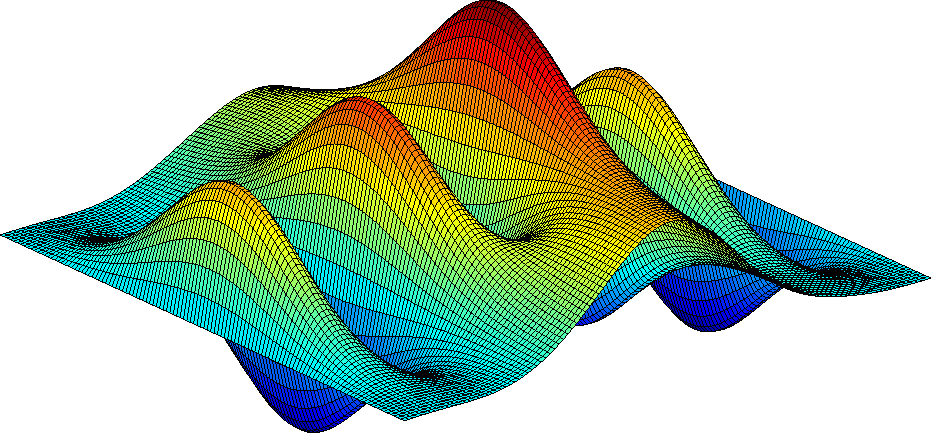
\includegraphics[width=6cm]{plotdata/plotgraphics3dsurf.png}}%
}

现在的关键思路是识别图像中的几个点，并\emph{同时}为它们分配逻辑三维坐标\emph{和}图像坐标中相应的二维画布坐标。如何做？嗯，三维坐标是 Matlab 已知的，如果你点击图像中的某个位置，它可以为你显示这些坐标，比较 Figure~\ref{fig:plotgraphics3d}（左）。


\begin{figure}
    \noindent
    \hbox to \linewidth{\hfill
        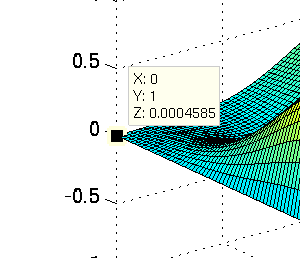
\includegraphics{plotdata/plotgraphics3dsurfmatlab.png}%
        \hfill
        \begin{minipage}[b][4cm][c]{2.6cm}%
        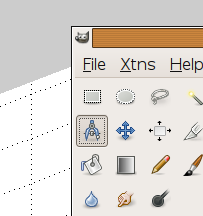
\includegraphics[width=\linewidth]{plotdata/plotgraphics_gimpmeasure.png}%
        \end{minipage}
        \hfill
    }
    \caption{使用 Matlab 提取图像坐标（左）和 Gimp 测量距离（右）。}
        \label{fig:plotgraphics3d}
\end{figure}


二维画布坐标需要一些工作；它们需要相对于图像的\emph{左下角}提供。我使用了 |gimp| 并将单位设为“Points”（左下角）。现在左下角以 |pt| 显示图像坐标，这与 \PGFPlots{} 兼容。指向坐标的替代方法是测量工具；比较 Figure~\ref{fig:plotgraphics3d}（右）中 |gimp| 的“Measure”工具，它允许计算一条线的长度（在我们的情况下，是从左下角到目标点的长度）。

我在图形中选择了四个点，并记录了它们的二维图像坐标和三维逻辑坐标，如下所示：
%
\begin{codeexample}[]
\begin{tikzpicture}
\begin{axis}[
    grid=both,minor tick num=1,
    xlabel=$x$,ylabel=$y$,
]
    \addplot3 graphics [
        points={% important
            (0,1,0) => (0,207-112)
            (1,0,0) => (446,207-133)
            (0.5546,0.5042,1.825) => (236,207)
            (0,0,0) => (194,207-202)
        },
    ] {plotdata/plotgraphics3dsurf.png};
\end{axis}
\end{tikzpicture}
\end{codeexample}
%
这里，|points| 键以我们收集的坐标作为参数。它接受形式为 \meta{3d 逻辑坐标} | => | \meta{2d 画布坐标} 的映射序列。在我们的例子中，|(0,1,0)| 在 |.png| 文件中的 |(0,207-112)| 处被找到。请注意，我引入了差值，因为 |gimp| 从左上角计数，但 \PGFPlots{} 从左下角计数。

一旦收集了这四个点坐标，我们就在 \PGFPlots{} 坐标轴中得到 Matlab 的曲面图。你可以修改任何外观选项，包括不同的坐标轴 limits 或更多 |\addplot| 命令：
%
\begin{codeexample}[]
\begin{tikzpicture}
\begin{axis}[
    xmax=1.5,% extra limits
    grid=both,minor tick num=1,
    xlabel=$x$,ylabel=$y$,
]
    \addplot3 [surf] % 'surf': only used for legend
        graphics [
            points={
                (0,1,0) => (0,207-112)
                (1,0,0) => (446,207-133)
                (0.5546,0.5042,1.825) => (236,207)
                (0,0,0) => (194,207-202)
        },
    ] {plotdata/plotgraphics3dsurf.png};
        \addlegendentry{Graphics}

    \addplot3+ [only marks] coordinates {
        (0,1,0) (1,0,0)
        (0.5546,0.5042,1.825) (0,0,0)
    };
        \addlegendentry{Scatter}
\end{axis}
\end{tikzpicture}
\end{codeexample}
%
\noindent \PGFPlots{} 使用这四个输入点来计算适当的 |x|、|y| 和 |z| 单位向量（以及图形坐标中的原点）。这四个向量（每个有两个分量）可以作为一个大小为 $8\times 8$ 的线性方程组的结果来计算，这就是为什么你需要提供四个输入点（每个有两个坐标）。\PGFPlots{} 计算导入图形的单位向量，然后重新缩放结果，使其适合指定的 |width| 和 |height|。这种重新缩放尊重 |unit vector ratio|（更准确地说，它使用 |scale mode=scale uniformly| 而不是 |scale mode=stretch to fill|）。因此，更改包含投影图形的三维坐标轴视图的自由度比之前小得多。令人惊讶的是，你仍然可以更改坐标轴 limits 以及 |width| 和 |height|——\PGFPlots{} 会负责正确显示你导入的图形。从版本~1.6 开始，你还可以更改 |zmin| 和/或 |zmax|——\PGFPlots{} 会尽可能尊重你的更改。

下面是另一个例子。假设我们有以下三维可视化图形：

{\setlength{\fboxsep}{0pt}%
\centering%
\fbox{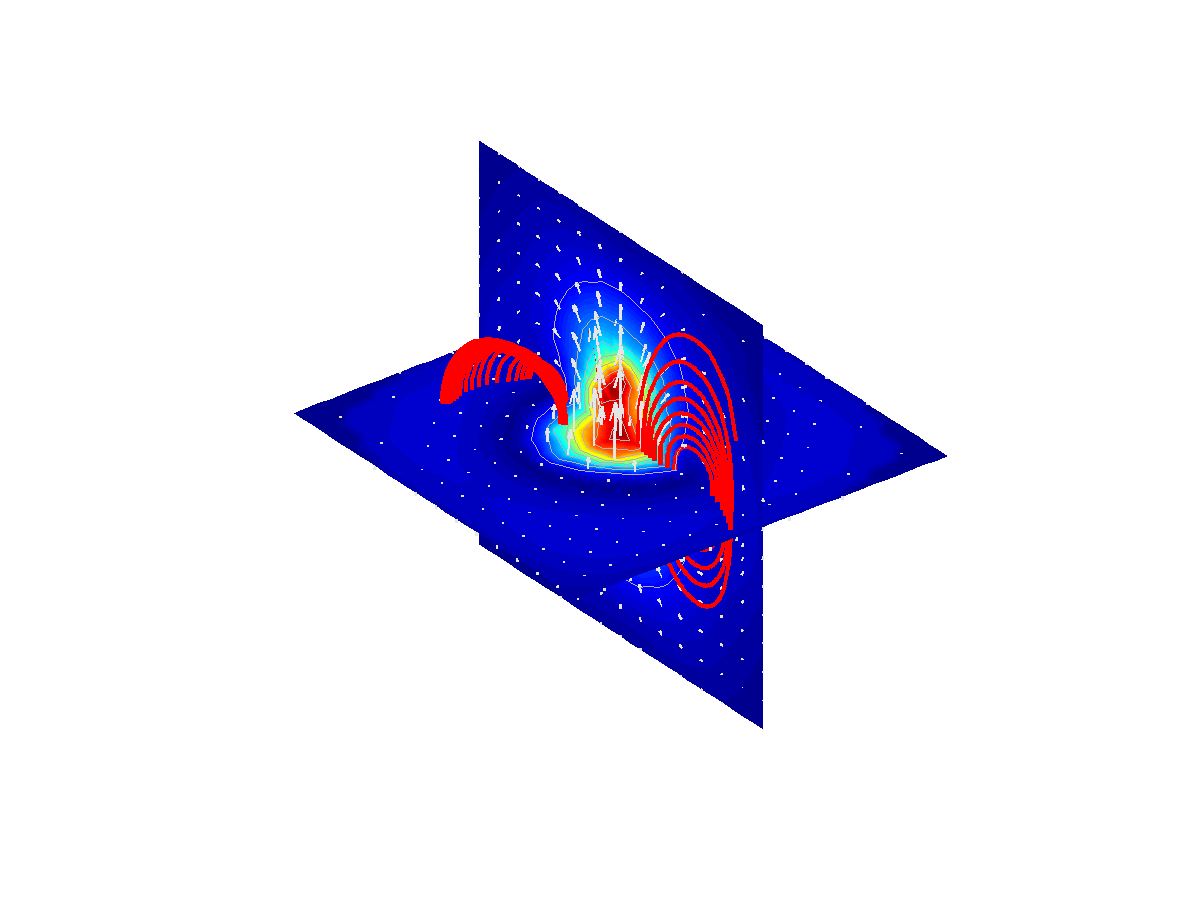
\includegraphics[width=6cm]{plotdata/risingdrop3d}}%
}

它由 Matlab 生成（我只用 |gimp| 为背景添加了透明度）。除了高级可视化技术之外，它还使用了 |axis equal|，即 |unit vector ratio=1 1 1|。和之前一样，我们需要识别四个点，每个点都有其三维逻辑坐标（来自 Matlab）以及相对于图形左下角的相关二维画布坐标（请注意图形周围有大量空白）。以下是导入结果图形时 \PGFPlots{} 的输出：
%
\begin{codeexample}[]
\begin{tikzpicture}
\begin{axis}[
    grid=both,minor tick num=1,
    xlabel=$x$,ylabel=$y$,
    title={\centering
      Geometry provided by Sven Gro\ss, Bonn\\
      \url{http://www.igpm.rwth-aachen.de/DROPS}\\},
    title style={text width=6cm,font=\tiny},
]
    \addplot3 graphics [
        points={
            (-0.002625,0.002625,0) => (140,234)
            (0,0.00263,0.00263)    => (230,364)
            (0,-0.00263,-0.00263)  => (366,81)
            (0,-0.00263,0.00263)   => (366,276)
            (0.002625,0.002625,0.002625)
        },
    ] {plotdata/risingdrop3d.png};
\end{axis}
\end{tikzpicture}
\end{codeexample}
%
\noindent 请注意，我在这里提供了\emph{五个}三维坐标，但最后一项没有 |=>| 映射到二维画布坐标。因此，它仅用于更新边界框（详见 |points| 键的参考手册）。

上面的例子产生了一个相对较小的图像和大量“空白”。这是由于 \PGFPlots{} 的 |scale mode=scale uniformly| 实现：它决定最好的方法是放大相关的坐标轴 limits。这里，“最好的方法”意味着满足 |width|/|height| 约束，同时最小化地放大（从不缩小）坐标轴 limits。剩余的自由度是 |width|、|height| 和坐标轴 limits。在我们的例子中，更改 |width| 和 |height| 之间的比例可以改善显示：

\begin{codeexample}[]
\begin{tikzpicture}
\begin{axis}[
    height=8cm,width=7cm,% improve scaling manually
    grid=both,minor tick num=1,
    xlabel=$x$,ylabel=$y$,
    title={\centering
      Geometry provided by Sven Gro\ss, Bonn\\
      \url{http://www.igpm.rwth-aachen.de/DROPS}\\},
    title style={text width=6cm,font=\tiny},
]
    \addplot3 graphics [
        points={
            (-0.002625,0.002625,0) => (140,234)
            (0,0.00263,0.00263)    => (230,364)
            (0,-0.00263,-0.00263)  => (366,81)
            (0,-0.00263,0.00263)   => (366,276)
            (0.002625,0.002625,0.002625)
        },
    ] {plotdata/risingdrop3d.png};
\end{axis}
\end{tikzpicture}
\end{codeexample}
%
\noindent 发生的事情是，\PGFPlots{} 选择了一个\emph{单一}缩放因子，该因子应用于从 |points| 键推导出来的所有单位。这确保导入的图形正确地适合坐标轴。此外，\PGFPlots{} 会尽力满足剩余的约束。

关于 \PGFPlots{} 如何缩放坐标轴的完整描述可以在 |scale mode=scale uniformly| 的文档中找到。这里只是简要总结：\PGFPlots{} 假设规定的 |width| 和 |height| 必须被满足。为此，它重新缩放投影的单位向量（即 $x$、$y$ 和 $z$ 中每个单位所占用的空间），并且可以修改坐标轴 limits。在默认配置 |scale uniformly strategy=auto| 中，\PGFPlots{} \emph{从不}缩小坐标轴 limits。


\paragraph{兼容性说明：}

请注意，\PGFPlots{} 版本~1.6 的缩放能力已得到改进。在以前的版本中，只有 |scale uniformly strategy=change vertical limits| 可用，这会导致坐标轴被裁剪。简而言之：请考虑在文档中写入 |\pgfplotsset{compat=1.6}| 或更新版本，以受益于改进的缩放。如果你使用 |\pgfplotsset{compat=1.5}| 或更早版本，|\addplot3 graphics| 的结果会有所不同。

我们来看第三个例子，它由以下 Matlab 代码生成：
%
\begin{codeexample}[code only]
clear all
close all
seed = sum(clock)
rand('seed',seed);
X = rand(10,10,10);
data = smooth3(X,'box',5);
p1 = patch(isosurface(data,.5), ...
   'FaceColor','blue','EdgeColor','none');
p2 = patch(isocaps(data,.5), ...
    'FaceColor','interp','EdgeColor','none');
isonormals(data,p1)
daspect([1 2 2])
view(3); axis vis3d tight
camlight; lighting phong
% print -dpng plotgraphics3withaxis
axis off
print -dpng plotgraphics3
save  plotgraphics3.seed seed -ASCII % to reproduce the result
\end{codeexample}
%
\noindent 我只用 |gimp| 添加了背景透明度，得到以下图形：

{\setlength{\fboxsep}{0pt}%
\centering%
\fbox{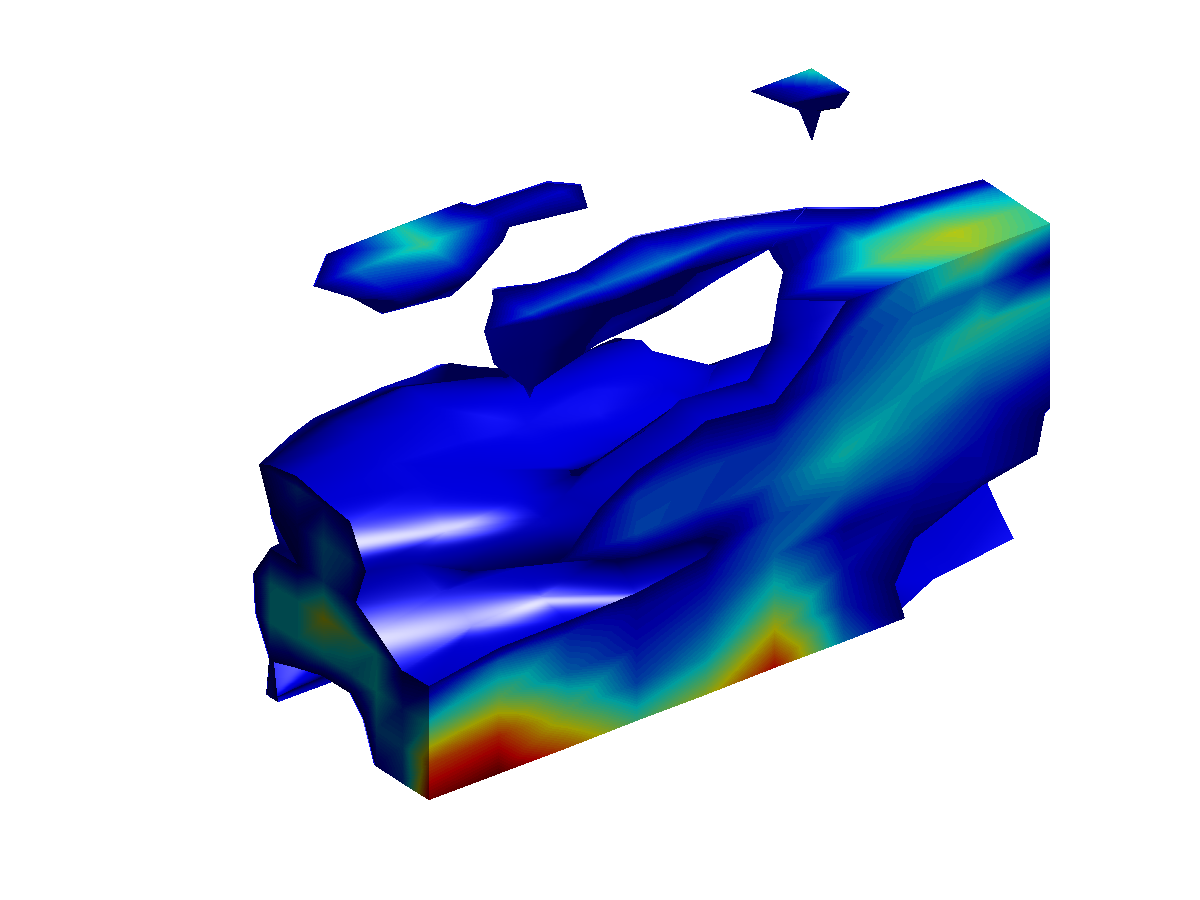
\includegraphics[width=6cm]{plotdata/plotgraphics3.png}}%
}

我们像之前一样继续，收集四个点，每个点都有三维逻辑坐标（通过点击 Matlab 图形）以及使用 gimp 测量工具得到的相关二维画布（图形）坐标。结果如下面的代码示例所示。
%
\begin{codeexample}[]
\begin{tikzpicture}
\begin{axis}[
    grid=both,minor tick num=1,
    xlabel=$x$,ylabel=$y$,
    3d box,
]
    \addplot3 graphics [
        points={
            (1,1,1)    => (205,48)
            (10,1,10)  => (503,324)
            (1,1,4.044)=> (206,102)
            (10,10,10) => (390,398)
        },
    ] {plotdata/plotgraphics3.png};
\end{axis}
\end{tikzpicture}
\end{codeexample}
%
\noindent 请注意，它具有非标准的数据纵横比，\PGFPlots{} 会自动尊重这一点。


\subsection*{外部三维图形与 Matlab}
\label{sec:plotgraphics3d:matlabscript}

\textit{由 Jürnjakob Dugge 提供的扩展} \vskip\baselineskip

\noindent 将三维逻辑坐标映射到二维画布坐标的过程很繁琐。

Jürnjakob Dugge 贡献了一个脚本，它完成了大部分逻辑工作，你的工作简化为复制--粘贴。经他允许，我在此发布该贡献。

其思路是启动一个简单的脚本，它会\emph{记录}用户点击的任何坐标的映射。工作方式如下：
%
\begin{enumerate}
    \item 创建 Matlab 图，例如使用
        %
\begin{codeexample}[code only]
hist3(randn(10000,2)) % some random data
set(get(gca,'child'),'FaceColor','interp','CDataMode','auto'); % colors
% make sure the "print" paper format is the same as the screen paper format:
set(gcf,'PaperPositionMode','auto')
\end{codeexample}
        %
    \item 将以下代码保存为 |pgfplotscsconversion.m|：
        %
\begin{codeexample}[code only]
function pgfplotscsconversion

% Hook into the Data Cursor "click" event
h = datacursormode(gcf);
set(h,'UpdateFcn',@myupdatefcn,'SnapToDataVertex','off');
datacursormode on

% select four points in plot using mouse

% The function that gets called on each Data Cursor click
function [txt] = myupdatefcn(obj,event_obj)

% Get the screen resolution, in dots per inch
dpi = get(0,'ScreenPixelsPerInch');

% Get the click position in pixels, relative to the lower left of the
% screen
screen_location=get(0,'PointerLocation');

% Get the position of the plot window, relative to the lower left of
% the screen
figurePos = get(gcf,'Position');

% Get the data coordinates of the cursor
pos = get(event_obj,'Position');

% Format the data and figure coordinates. The factor "72.27/dpi" is
% necessary to convert from pixels to TeX points (72.27 points per inch)
display(['(',num2str(pos(1)),',',num2str(pos(2)),',',num2str(pos(3)),') => (', ...
   num2str((screen_location(1)-figurePos(1))*72.27/dpi),',', ...
   num2str((screen_location(2)-figurePos(2))*72.27/dpi),')'])

% Format the tooltip display
txt = {['X: ',num2str(pos(1))],['Y: ',num2str(pos(2))],['Z: ',num2str(pos(3))]};
\end{codeexample}
        %
        运行 |pgfplotscsconversion|，在你的图上点击四个点。最好选择靠近图边缘的非共线点。复制并粘贴写入 Matlab 命令窗口的四行内容。

        确保前两个点在屏幕上具有不同的 $X$ 和 $Y$ 值（即图像画布坐标）。
    \item 将图导出为图像
        %
\begin{codeexample}[code only]
axis off
print -dpng matlabout -r400 % PNG called "matlabout.png" with 400 dpi resolution
\end{codeexample}

        如果你想导出矢量图形，应该注意 Matlab 的 |pdf| 输出比较笨拙。最好先导出为 |eps|，然后再从 |eps| 转换为 |pdf|。

        \emph{如果}你真的想使用 Matlab 的 |pdf| 输出，可能需要自己设置纸张大小以匹配图形大小，因为 PDF 驱动程序不会自动调整大小：
        %
\begin{codeexample}[code only]
% It might be better to use print -depsc followed by epstopdf.
% Use this if you (really) want to use print -dpdf:
currentScreenUnits=get(gcf,'Units')     % Get current screen units
currentPaperUnits=get(gcf,'PaperUnits') % Get current paper units
set(gcf,'Units',currentPaperUnits)      % Set screen units to paper units
plotPosition=get(gcf,'Position')        % Get the figure position and size
set(gcf,'PaperSize',plotPosition(3:4))  % Set the paper size to the figure size
set(gcf,'Units',currentScreenUnits)     % Restore the screen units

print -dpdf matlabout      % PDF called "matlabout.pdf"
\end{codeexample}
        %
    \item 将图像包含到你的 \PGFPlots{} 坐标轴中。如果你在图的角上选择了点，你的 |xmin|、|xmax|、|ymin| 和 |ymax| 应该会被自动设置，否则你可能需要自己提供这些值。此外，调整 |width| 和 |height| 可能有助于获得正确的图垂直位置。考虑更改 |zmin| 和/或 |zmax| 以满足你的需求（最好只更改其中一个；否则 \PGFPlots{} 可能无法固定 |height|）。
\end{enumerate}

此贡献来自

\noindent
\url{http://tex.stackexchange.com/questions/52987/3-dimensional-histogram-in-pgfplots} .


\subsection*{总结：外部三维图形}

如前几节所示，\verbpdfref{\addplot3} |graphics| 允许包含三维图形，而 \PGFPlots{} 以其全部能力叠加一个灵活的坐标轴。这样做的代价是：
%
\begin{enumerate}
    \item 为你的图形\emph{四个点}收集逻辑三维坐标\emph{和}图像内部二维坐标。

        在 Matlab 中，可以通过第~\pageref{sec:plotgraphics3d:matlabscript} 页提到的工具来简化。
    \item 如果你的坐标轴构成右手坐标系，那就完成了。如果不是，还要为任何反向的坐标轴添加 |x dir=reverse|。
\end{enumerate}

\noindent 如果你在使用 \verbpdfref{\addplot3} |graphics| 时遇到问题，请考虑以下列表：
%
\begin{itemize}
    \item 必须能够从提供的四个 |points| 推导出原点和三个（二维）单位向量；否则算法将失败。

        算法应该能检测到任何缺陷。不过，如果你在这里遇到奇怪的“Dimension too large”消息，可以尝试 |points| 中的其他参数。查看你的日志文件，它可能会指出问题的根源（或使用 |debug| 键）。
    \item 确保外部图形具有正交坐标轴。事实上，坐标轴可以是倾斜的（就像 \PGFPlots{} 坐标轴可以通过自定义 |x|、|y| 和 |z| 向量创建一样）。不过，外部图像不能有透视投影，因为 \PGFPlots{} 不支持这种。|points| 命令需要接收四个属于线性无关位置向量的点。
    \item \PGFPlots{} 使用前两个点将图形挤压到所需坐标中（这意味着它们不应具有相同的画布 $X$ 或 $Y$ 坐标）。它会验证剩余的 |points| 参数是否被正确投影。
    \item 通过 |scale mode=scale uniformly| 产生的缩放将尝试满足所有缩放约束。你可以通过修改 |width|、|height|、|xmin|、|xmax|、|ymin|、|ymax|、|zmin|、|zmax| 和/或这些参数的任意组合来更改这些约束。另见 |unit rescale keep size|，它控制 limits 更改的灵活性。还有一个键 |scale uniformly strategy|，它允许选择不同的缩放策略。
    \item 图像应该具有“右手坐标系”：你应该能够用右手，拇指指向 $x$ 轴方向，食指指向~$y$ 方向，中指指向 $z$ 轴方向。如果不可能，说明你的某个坐标轴是反向的，你需要通过 |x dir=reverse| 键（及其变体）显式告知 \PGFPlots{}。
    \item 请注意，此功能仅在标准笛卡尔坐标轴上经过验证。
    \item 有一个 |debug| 键可用于调查算法在做什么：
        %
        \begin{pgfplotskey}{plot graphics/debug=\mchoice{true,false,visual} (initially false)}
            如果你提供 |\addplot3 graphics[debug,points={...}]|，\PGFPlots{} 将在你的终端和日志文件中提供调试信息。它还会生成额外的文件，其中包含确定的单位向量和用于推导它们的线性方程组（每个 |\addplot3 graphics| 语句生成一个这样的文件，文件名将是图形文件名加上 |.dat|）。

            如果没有 |debug| 键，只有日志文件会包含关于 \PGFPlots{} 在幕后做什么的简要信息。

            选择 \declaretext{true} 会激活日志消息。选择 \declaretext{visual} 会激活日志消息\emph{并}在提供的 |points| 处放置一些实心圆。选择 \declaretext{false} 会禁用所有 |debug| 功能。
        \end{pgfplotskey}
\end{itemize}
}


\subsection{从文件读取坐标}

\begin{addplotoperation}[]{file}{\marg{name}}
\labelprefix\label{pgfplots:addplot:file}

    \paragraph{弃用说明：}

    如果你有数据文件，通常应该使用 |\addplot table|。输入类型 |\addplot file| 几乎相同，但功能要弱得多。它仅为向后兼容而保留。

    |\addplot file| 输入机制类似于 \Tikz{} 命令 `|\addplot file|'。它应这样使用：

\begin{codeexample}[code only]
\addplot file {datafile.dat};
\end{codeexample}
    %
    其中 \meta{name} 是一个至少有两列的文本文件，这些列将用作 $x$ 和 $y$ 坐标。以 `|%|' 或 `|#|' 开头的行会被忽略。此类文件通常由 \textsc{gnuplot} 生成：
    %
\begin{codeexample}[code only]
#Curve 0, 20 points
#x y type
0.00000 0.00000 i
0.52632 0.50235 i
1.05263 0.86873 i
1.57895 0.99997 i
...
9.47368 -0.04889 i
10.00000 -0.54402 i
\end{codeexample}
    %
    此列表复制自~\cite[Section~16.4]{tikz}。

    Plot file 接受一个可选参数，

\begin{codeexample}[code only]
\addplot file [skip first] {datafile.dat};
\end{codeexample}

    \noindent 它允许跳过一个非注释标题行。这允许通过跳过列名来读取与 |\addplot table| 相同的输入文件。请注意，注释行在这里不计为行。

    输入方法 |\addplot file| 还可以为每个坐标读取元数据。如 |\addplot coordinates| 中已经解释的（见上文），元数据可以用于单独更改每个标记的颜色或其他样式参数。现在，如果 |point meta| 设置为 |explicit| 或 |explicit symbolic|，并且输入方法是 |\addplot file|，则将从磁盘读取一个额外元素——对每一行。元数据始终是读取的最后一个元素。关于逐点元数据的信息和示例见第~\pageref{pgfplots:scatter:src} 页，使用 |scatter/classes| 的应用示例见第~\pageref{pgfplots:scatterclasses} 页。

    Plot file 与 |\addplot table| 非常相似：你可以用以下方式达到相同的效果：
    %
\begin{codeexample}[code only]
\addplot table [x index=0,y index=1,header=false] {datafile.dat};
\end{codeexample}
    %
    \noindent 由于其简单性，|\addplot file| 稍快一些，而 |\addplot table| 允许更高的灵活性。

    技术说明：每个打开的文件都会被记录到你的日志文件中。

    文件可以包含 |empty line|，以告诉 \PGFPlots{} 函数有跳跃。要使用它，只需插入一个空行（并确保你的导言区中有 |\pgfplotsset{compat=1.4}| 或更新版本）。详见 |empty line| 的文档。
\end{addplotoperation}

\begin{pgfplotskeylist}{%
    plot file/skip first=\mchoice{true,false} (initially false),
    plot file/ignore first=\mchoice{true,false} (initially false)%
}
    这两个键可以作为 |\addplot file[|\meta{options}|] |\marg{filename}|;| 的参数提供，以跳过文件中第一个非注释条目。它们是等价的。如果你在此上下文中提供它们，则可以省略前缀 |/pgfplots/plot file|。
\end{pgfplotskeylist}


\section{关于选项：预备知识}

\PGFPlots{} 提供了大量键值选项，它们可以被（重新）定义以启用所需的功能，或被修改以进行某些微调。

一个键通常带有一个值（例如一个数字、一个字符串，或者某些宏代码）。你可以在 \LaTeX{} 文档中的许多位置为键赋值（即“设置键”）。该值将一直有效，直到它被更改，或者直到当前 \TeX{} 作用域结束（作用域结束发生在遇到闭花括号 `|}|'、|\end|\marg{name} 之后，或者例如在 |\addplot| 之后）。

\noindent 大多数键可以如下使用
%
\begin{codeexample}[code only]
\begin{tikzpicture}
\begin{axis}[key=value,key2=value2] % axis-wide keys
...
\end{axis}
\end{tikzpicture}
\end{codeexample}
%
\noindent 这会将更改应用于整个坐标轴。在此上下文中，|key| 可以是本手册中定义的任何选项，无论它带有 |/pgfplots/| 还是 |/tikz/| 键前缀。请注意，在几乎所有情况下都可以省略键前缀。

通常，值可以不写花括号。例如，如果手册中有类似 `|xmin=|\marg{$x$-coordinate}' 的内容，你可以放心地省略花括号。当值包含会使键设置产生歧义的内容（例如等号 `|=|' 或逗号 `|,|'）时，花括号是必需的。

有些键可以为每一张图单独修改：
%
\begin{codeexample}[code only]
\begin{tikzpicture}
    \begin{axis}
        % keys valid for single plots:
        \addplot ... ;                          % uses the "cycle list" to determine keys
        \addplot [key=value,key2=value2] ... ;  % uses the provided keys (not the "cycle list")
        \addplot+ [key=value,key2=value2] ... ; % appends something to the "cycle list"
    \end{axis}
\end{tikzpicture}
\end{codeexample}

除了这两种方式之外，还可以使用文档级的键：
%
\begin{codeexample}[code only]
\chapter{My Chapter}
\pgfplotsset{
    key=value,
    key2=value2,
}
This chapter has a common key configuration:
\begin{tikzpicture}
    \begin{axis}% uses the key config from above
    ...
    \end{axis}
\end{tikzpicture}
\end{codeexample}
%
\noindent 在上面的例子中，|\pgfplotsset| 命令用于修改键。这些更改是永久性的，将一直有效，直到
%
\begin{itemize}
    \item 你重新定义它们，或者
    \item 当前环境（例如 |\end{figure}|）结束，或者
    \item \TeX{} 遇到闭花括号 `|}|'。
\end{itemize}
%
这包括文档全局导言区的配置，例如
%
\begin{codeexample}[code only]
\documentclass{article}

\usepackage{pgfplots}
\pgfplotsset{
    xticklabel={$\mathsf{\pgfmathprintnumber{\tick}}$},
    every axis/.append style={
        font=\sffamily,
    },
}
...
\end{codeexample}

管理键值对的基本引擎是 |pgfkeys|，它是 \pgfname{} 的一部分。该引擎总是带有一个键名和一个键“路径”，这有点类似于文件的文件名和目录。\PGFPlots{} 的公共“目录”（键路径）是 `|/pgfplots/|'。尽管下面的键定义提供了完整路径，但省略该前缀总是（好吧，几乎总是）安全的——\PGFPlots{} 会自动使用它。对于 \Tikz{} 绘图选项通用的前缀 `|/tikz/|'，以及用于 \pgfname{}（或多或少）底层命令的前缀 `|/pgf/|'，情况也是如此。所有这些前缀都可以省略。

一个重要的概念是 \emph{样式} 的概念。样式是一个包含一个或多个其他键的键。它可以被重新定义或修改，直到被内部例程实际使用。\Tikz{} 和 \PGFPlots{} 的每一个单独组件都可以通过样式进行配置。

例如，
%
\begin{codeexample}[code only]
\pgfplotsset{legend style={line width=1pt}}
\end{codeexample}
%
\noindent 通过向现有的图例样式追加 `|line width=1pt|'，将每个图例的线宽设置为 |1pt|。

有些键，例如 |legend style|、|ticklabel style| 和 |label style|，允许修改预定义样式（在本例中分别是图例、刻度标签和坐标轴标签的样式）。它们通常等价于 \meta{style name}|/.append style={}| 命令（唯一的区别是 |/.append style| 这种写法稍微长一点）。还可以使用 |/.style={}| 来定义新样式（或覆盖已有的样式）。

还有一些其他预定义样式可用于修改外观，参见 Section~\ref{sec:styles}。

\begin{command}{\pgfplotsset\marg{key-value-list}}
    定义或设置 \meta{key-value-list} 中的所有选项。\meta{key-value-list} 可以包含本手册中任何带有 |/pgfplots/| 前缀的选项（不过你不需要输入该前缀）。

    在 \meta{key-value-list} 内部，本手册中常见的前缀 `|/pgfplots/|' 可以省略（它们会被自动检查）。

    此命令可用于为整个文档或文档的某一部分定义默认选项。例如，
    %
\begin{codeexample}[code only]
\pgfplotsset{
    cycle list={
        {red, mark=*},          {blue,mark=*},
        {red, mark=x},          {blue,mark=x},
        {red, mark=square*},    {blue,mark=square*},
        {red, mark=triangle*},  {blue,mark=triangle*},
        {red, mark=diamond*},   {blue,mark=diamond*},
        {red, mark=pentagon*},  {blue,mark=pentagon*}
    },
    legend style={
        at={(0.5,-0.2)},
        anchor=north,
        legend columns=2,
        cells={anchor=west},
        font=\footnotesize,
        rounded corners=2pt,
    },
    xlabel=$x$,
    ylabel=$f(x)$,
}
\end{codeexample}
    %
    可用于为整本文档设置线型规格、图例样式和坐标轴标签的文档级样式。这些设置将一直有效，直到当前环境（例如 |\end{figure}|）结束，或者你重新定义它们，或者遇到下一个闭花括号 `|}|'（以先到者为准）。

    你还可以使用 |/.style| 和 |/.append style| 定义新样式（键值对的集合）。
    %
\begin{codeexample}[code only]
\pgfplotsset{
    My Style 1/.style={xlabel=$x$, legend entries={1,2,3} },
    My Style 2/.style={xlabel=$X$, legend entries={4,5,6} }
}
\end{codeexample}
    %
    |/.style| 和 |/.append style| 这两个键处理器在 Section~\ref{sec:styles} 中有更详细的描述。
\end{command}

\begin{handler}{{.code}=\marg{\TeX{} code}}
    有时，\PGFPlots{} 的用户界面会提供替换其部分例程的功能。这是通过所谓的“代码键”来实现的。其含义是用新的 \meta{\TeX{} 代码} 替换原来的键及其行为。在 \meta{\TeX{} 代码} 内部，可以使用任何命令。此外，|#1| 模式将是传递给该键的参数。

\begin{codeexample}[]
\pgfplotsset{
    My Code/.code={I've been invoked with `#1'}}
\pgfplotsset{My Code={this here}}
\end{codeexample}
    %
    该例子定义了一个（新的）名为 |My Code| 的键。本质上，它不过是一个 |\newcommand|，被接入到了键值接口中。第二条语句“调用”了这个代码键。
\end{handler}

\begin{handler}{{.code 2 args}=\marg{\TeX{} code}}
    与 |/.code| 类似，但此处理器定义的键接受两个参数。当使用这样定义的键时，这两个参数可通过 |#1| 和 |#2| 获取。
\end{handler}

\begin{handler}{{.cd}}
    每个键都有一个带（长）前缀的完全限定名，例如 |/pgfplots/xmin|。然而，如果“当前目录”是 |/pgfplots|，那么只写 |xmin| 就足够了。|/.cd| 键处理器就是以这种方式更改“当前目录”的。

    对于传递给 |\begin{axis}|\oarg{options} 或 |\addplot| 的任何参数，会自动检查前缀 |/tikz/| 和 |/pgfplots/|。因此，你无需担心它们，直接省略即可——如果宏包未能识别该选项，再仔细检查。
\end{handler}


\subsection{\textsc{PGFPlots} 与 \Tikz{} 选项}

本节或多或少偏技术性，除非你确实想了解更多关于此主题的内容，否则可以跳过。

\Tikz{} 选项和 \PGFPlots{} 选项可以在坐标轴参数中以及任何相关样式中混用。例如，
%
\begin{codeexample}[code only]
\pgfplotsset{every axis legend/.append style={
    legend columns=3,font=\Large},
}
\end{codeexample}
%
\noindent 同时指定了 `|legend columns|' 选项（一个 \PGFPlots{} 选项），并使用 `|font|' 来绘制图例（一个 \Tikz{} 选项）。关键在于：|legend columns| 需要在图例排版 \emph{之前} 就已知，而 |font| 则需要在图例排版时生效。\PGFPlots{} 会自动理清所有键之间的依赖关系：

坐标轴环境会处理任何已知的 \PGFPlots{} 选项，并且所有 `|every|' 样式都会被解析以查找 \PGFPlots{} 选项。每个未知的选项都被假定为 \Tikz{} 选项，并会被转发给相应的 \Tikz{} 绘图命令。例如，上面的 `|font=\Large|' 将被用作图例矩阵的参数，而下面这段中的 `|font=\Large|' 参数
%
\begin{codeexample}[code only]
\pgfplotsset{every axis label/.append style={
    ylabel=Error,xlabel=Dof,font=\Large},
}
\end{codeexample}
%
将被用于坐标轴标签的节点中（但不会用于坐标轴标题，例如）。

如果你给坐标轴标签指定了不兼容的选项，那将是一个错误，例如 `|xmin|' 和 `|xmax|' 不能在 `|every axis label|' 内部设置。


\section{二维图类型}

{%
\tikzset{external/figure name/.add={}{twodim_}}

\PGFPlots{} 支持多种二维线图，例如分段线性线图、分段常值图、平滑图、
柱状图和梳状图。其中大多数直接使用 \PGF{} 的 plot handler 库，参见
\cite[Section~18.8]{tikz}。

图类型是绘图样式的一部分，因此通过选项来设置。大多数基本二维图类型
属于 \Tikz{}，参见 \cite[Section~18.8]{tikz}，\Tikz{} 用户可能已经
熟悉它们。这里也对它们进行文档说明。


\subsection{线性图}

\begin{plottype}{sharp plot}
    线性（"折线"）图是默认值。点坐标之间简单地用直线连接。
\begin{codeexample}[]
\begin{tikzpicture}
\begin{axis}
    \addplot+ [
        sharp plot,
    ] coordinates {
        (0,0) (1,2) (2,3)
    };
\end{axis}
\end{tikzpicture}
\end{codeexample}

    这里的 `|+|' 表示使用正常的绘图循环列表，并将 `|sharp plot|'
    附加到其选项列表中。
\end{plottype}


\subsection{平滑图}

\begin{plottype}{smooth}
    平滑图在相邻点之间进行平滑插值。
\begin{codeexample}[]
\begin{tikzpicture}
\begin{axis}
    \addplot+ [
        smooth,
    ] coordinates {
        (0,0) (1,2) (2,3)
    };
\end{axis}
\end{tikzpicture}
\end{codeexample}
\end{plottype}

正如~\cite{tikz} 中详细描述的那样，这个 plot handler 会产生一个
"平滑"的轮廓。然而，它"并不十分智能"（比较~\cite{tikz}），与常见的
基于绘图的插值方案无关。

\begin{key}{/tikz/tension=\marg{tension} (initially 0.55)}
    一个控制如何确定剩余自由度的参数：它控制平滑效果。较高的值会产生
    更"圆润"的角，而较低的值会产生尖角。

    详情请参阅~\cite{tikz}。
\end{key}


\subsection{常值图}

常值图绘制平行于 $x$ 轴的线来连接坐标。不连续的边可以绘制或不绘制，
标记可以放置在左端或右端。

\begin{plottype}{const plot}
    用水平线和竖直线连接所有点。标记放置在线段的左端，使绘图在所有
    数据点处右连续。

\begin{codeexample}[]
\begin{tikzpicture}
\begin{axis}
    \addplot+ [
        const plot,
    ] coordinates {
        (0,0.1)    (0.1,0.15)  (0.2,0.5)   (0.3,0.62)
        (0.4,0.56) (0.5,0.58)  (0.6,0.65)  (0.7,0.6)
        (0.8,0.58) (0.9,0.55)  (1,0.52)
    };
\end{axis}
\end{tikzpicture}
\end{codeexample}


\begin{codeexample}[]
\begin{tikzpicture}
\begin{axis}[ymin=0,ymax=1,enlargelimits=false]
    \addplot [
        const plot,
        fill=blue,
        draw=black,
    ] coordinates {
        (0,0.1)    (0.1,0.15)  (0.2,0.5)   (0.3,0.62)
        (0.4,0.56) (0.5,0.58)  (0.6,0.65)  (0.7,0.6)
        (0.8,0.58) (0.9,0.55)  (1,0.52)
    }
        \closedcycle
    ;
\end{axis}
\end{tikzpicture}
\end{codeexample}
\end{plottype}

\begin{plottype}{const plot mark left}
    `|const plot|' 的别名。
\end{plottype}

\begin{plottype}{const plot mark right}
    一个变体，将标记放置在每个线段的右端，使绘图在给定坐标处左连续。
    %
\begin{codeexample}[]
\begin{tikzpicture}
\begin{axis}
    \addplot+ [
        const plot mark right,
    ] coordinates {
        (0,0.1)    (0.1,0.15)  (0.2,0.5)   (0.3,0.62)
        (0.4,0.56) (0.5,0.58)  (0.6,0.65)  (0.7,0.6)
        (0.8,0.58) (0.9,0.55)  (1,0.52)
    };
\end{axis}
\end{tikzpicture}
\end{codeexample}
\end{plottype}

\begin{plottype}{const plot mark mid}
    一个变体，将标记放置在每个线段的中间，使绘图关于其数据点对称。
    %
\begin{codeexample}[]
\begin{tikzpicture}
\begin{axis}
    \addplot+ [
        const plot mark mid,
    ] coordinates {
        (0,0.1)    (0.1,0.15)  (0.2,0.5)   (0.3,0.62)
        (0.4,0.56) (0.5,0.58)  (0.6,0.65)  (0.7,0.6)
        (0.8,0.58) (0.9,0.55)  (1,0.52)
    };
\end{axis}
\end{tikzpicture}
\end{codeexample}
    %
    注意，"对称"仅对恒定的网格间距成立：如果相邻数据点之间的 $x$
    距离不同，|const plot mark mid| 会在每对连续点之间的中间位置绘制
    竖直线。
\end{plottype}

\begin{plottype}{jump mark left}
    `|const plot mark left|' 的一个变体，不绘制竖直线。
    %
\begin{codeexample}[]
\begin{tikzpicture}
\begin{axis}[samples=8]
    \addplot+ [
        jump mark left,
        domain=-5:0,
    ] {4*x^2 - 5};

    \addplot+ [
        jump mark right,
        domain=-5:0,
    ] {0.7*x^3 + 50};
\end{axis}
\end{tikzpicture}
\end{codeexample}
\end{plottype}

\begin{plottype}{jump mark right}
    `|const plot mark right|' 的一个变体，不绘制竖直线。
\end{plottype}

\begin{plottype}{jump mark mid}
    `|const plot mark mid|' 的一个变体，不绘制竖直线。
    %
\begin{codeexample}[]
\begin{tikzpicture}
\begin{axis}
    \addplot+ [
        jump mark mid,
    ] coordinates {
        (0,0.1)    (0.1,0.15)  (0.2,0.5)   (0.3,0.62)
        (0.4,0.56) (0.5,0.58)  (0.6,0.65)  (0.7,0.6)
        (0.8,0.58) (0.9,0.55)  (1,0.52)
    };
\end{axis}
\end{tikzpicture}
\end{codeexample}
\end{plottype}


\subsection{柱状图}

柱状图在坐标处放置水平或垂直的柱。同一坐标轴中的多个柱状图可以堆叠
在一起，也可以并排排列。

\begin{plottype}{xbar}
    在 $(y=0)$ 线与每个坐标之间放置水平柱。

    此选项按每个绘图单独使用，仅配置坐标的可视化方式。图级别的样式
    |/pgfplots/xbar| 还会为刻度、图例和多个绘图设置合理的选项。
    %
\begin{codeexample}[]
\begin{tikzpicture}
\begin{axis}
    \addplot+ [
        xbar,
    ] coordinates {
        (4,0) (1,1) (2,2)
        (5,3) (6,4) (1,5)
    };
\end{axis}
\end{tikzpicture}
\end{codeexample}
    %
    柱以绘图坐标为中心，宽度为 |bar width|。使用柱状图通常不仅仅意味着
    连接坐标的方式不同，例如将刻度绘制在坐标轴外侧、改变图例的外观，
    或者在出现多个 |\addplot| 命令时引入偏移。

    对于 |xbar|，有一个预配置的样式：如果你将 |xbar| 作为参数提供给
    坐标轴环境，它会自动安装并提供此功能。
    %
% \usetikzlibrary{patterns}
\begin{codeexample}[]
\begin{tikzpicture}
\begin{axis}[xbar,enlargelimits=0.15]
    \addplot [draw=blue,
        pattern=horizontal lines light blue,
    ] coordinates {
        (10,5) (15,10) (5,15) (24,20) (30,25)
    };
    \addplot [draw=black,
        pattern=horizontal lines dark blue,
    ] coordinates {
        (3,5) (5,10) (15,15) (20,20) (35,25)
    };
\end{axis}
\end{tikzpicture}
\end{codeexample}
    %
    这里 |xbar| 产生 |/pgfplots/xbar|，因为它是坐标轴的参数，
    而不是单个绘图的参数。

    对于柱状图，在柱附近提供文本坐标甚至描述性节点是很常见的。
    这可以分别使用 |symbolic y coords| 和 |nodes near coords| 键来实现：
    %
\begin{codeexample}[]
\begin{tikzpicture}
    \begin{axis}[
        xbar, xmin=0,
        width=12cm, height=3.5cm, enlarge y limits=0.5,
        xlabel={\#participants},
        symbolic y coords={no,yes},
        ytick=data,
        nodes near coords, nodes near coords align={horizontal},
    ]
        \addplot coordinates {(3,no) (7,yes)};
    \end{axis}
\end{tikzpicture}
\end{codeexample}
    %
    |symbolic y coords| 定义了一个可接受坐标的字典，这些坐标随后将作为
    $y$ 坐标使用；而 |nodes near coords| 键将值显示为额外的节点
    （详情参见它们的参考文档）。该示例使用了 |enlarge y limits| 以获得
    更多空闲空间，因为默认间距并不总是适合柱状图。

    注意，如上例中显式包含 |xmin=0| 可能相当重要。如果没有它，将使用
    下界：
    %
\begin{codeexample}[]
\begin{tikzpicture}
    \begin{axis}[
        title=Uses lowest $x$ coords for xmin,
        xbar,
        width=12cm, height=3.5cm, enlarge y limits=0.5,
        xlabel={\#participants},
        symbolic y coords={no,yes},
        ytick=data,
        nodes near coords, nodes near coords align={horizontal},
      ]
        \addplot coordinates {(1,no) (9,yes)};
    \end{axis}
\end{tikzpicture}
\end{codeexample}

    除了线、填充和颜色样式外，柱还可以用 |bar width| 和 |bar shift|
    进行配置，见下文。
\end{plottype}

\begin{stylekey}{/pgfplots/xbar=\marg{shift for multiple plots} (default 2pt)}
    此样式为整个坐标轴设置 |/tikz/xbar| \emph{以及}一些关于水平柱的常用
    选项。如果你将 |xbar| 作为坐标轴参数提供，这会自动完成，见上文。

    |xbar| 样式定义了当多个绘图放入同一坐标轴时的偏移。它将柱相邻绘制，
    彼此之间相隔 \meta{shift for multiple plots}。此外，它还设置了
    |bar cycle list| 样式，并设置了刻度和图例的外观选项。

    该样式定义如下。
    %
\begin{codeexample}[code only]
\pgfplotsset{
    /pgfplots/xbar/.style={
        /tikz/xbar,
        bar cycle list,
        tick align=outside,
        xbar legend,
        /pgfplots/bar shift auto={#1},
    },
}
\end{codeexample}

    \begin{pgfplotskey}{bar shift auto=\marg{shift for multiple plots} (default 2pt)}
        |bar shift| 的公式根据绘图总数和当前绘图的编号来分配偏移。
        它的设计目的是填充总宽度 $n \cdot $|bar width|$ + (n-1) \cdot $
        \meta{shift for multiple plots}。其中 $0.5$ 用于补偿居中。

        该样式定义为
        %
\begin{codeexample}[code only]
\pgfplotsset{
    /pgfplots/bar shift auto/.style={
        /pgf/bar shift={%
            % total width = n*w + (n-1)*skip
            % -> subtract half for centering
            -0.5*(\numplotsofactualtype*\pgfplotbarwidth + (\numplotsofactualtype-1)*(#1)) +
            % the '0.5*w' is for centering
            (.5+\plotnumofactualtype)*\pgfplotbarwidth + \plotnumofactualtype*(#1)},
    },
}
\end{codeexample}
    \end{pgfplotskey}
\end{stylekey}

\begin{plottype}{ybar}
    与 |xbar| 类似，此选项生成柱状图。它在 ($x=0$) 线与每个输入坐标
    之间绘制垂直柱。
    %
\begin{codeexample}[]
\begin{tikzpicture}
\begin{axis}
    \addplot+ [
        ybar,
    ] coordinates {
        (0,3) (1,2) (2,4) (3,1) (4,2)
    };
\end{axis}
\end{tikzpicture}
\end{codeexample}
    %
    上面的示例只是改变了输入坐标的可视化方式。正如 |xbar| 中提到的，
    通常需要为同一坐标轴中的多个柱修改图例和偏移。

    有一个预定义的样式，当提供给坐标轴环境时会安装这些自定义设置：
    %
\begin{codeexample}[]
\begin{tikzpicture}
\begin{axis}[
    x tick label style={
        /pgf/number format/1000 sep=},
    ylabel=Population,
    enlargelimits=0.15,
    legend style={at={(0.5,-0.15)},
        anchor=north,legend columns=-1},
    ybar,
    bar width=7pt,
]
    \addplot coordinates {
        (1930,50e6) (1940,33e6)
        (1950,40e6) (1960,50e6) (1970,70e6)
    };
    \addplot coordinates {
        (1930,38e6) (1940,42e6)
        (1950,43e6) (1960,45e6) (1970,65e6)
    };
    \addplot coordinates {
        (1930,15e6) (1940,12e6)
        (1950,13e6) (1960,25e6) (1970,35e6)
    };
    \addplot [red,line legend,
        sharp plot,update limits=false,
    ] coordinates { (1910,4.3e7) (1990,4.3e7) }
        node [above] at (1950,4.3e7) {Houses};

    \legend{Far,Near,Here,Annot}
\end{axis}
\end{tikzpicture}
\end{codeexample}
    %
    这里，|ybar| 产生 |/pgfplots/ybar|，因为它是坐标轴的参数，
    而不是单个绘图的参数。该样式影响前三个 |\addplot| 命令。注意它会
    在绘图坐标周围水平移动它们。第四个 |\addplot| 命令是某种注释，
    它不 |update limits|。

    |ybar| 样式可以以与 |xbar| 中描述类似的方式与 |symbolic x coords|
    结合使用：
    %
\begin{codeexample}[]
\begin{tikzpicture}
\begin{axis}[
    ybar,
    enlargelimits=0.15,
    legend style={at={(0.5,-0.15)},
    anchor=north,legend columns=-1},
    ylabel={\#participants},
    symbolic x coords={tool8,tool9,tool10},
    xtick=data,
    nodes near coords,
    nodes near coords align={vertical},
]
\addplot coordinates {(tool8,7) (tool9,9) (tool10,4)};
\addplot coordinates {(tool8,4) (tool9,4) (tool10,4)};
\addplot coordinates {(tool8,1) (tool9,1) (tool10,1)};
    \legend{used,understood,not understood}
\end{axis}
\end{tikzpicture}
\end{codeexample}

    与 |xbar| 一样，柱宽和偏移可以用 |bar width| 和 |bar shift| 配置。
    但是，柱偏移最好作为 |/pgfplots/ybar| 的参数提供，因为该样式会
    覆盖柱偏移。因此，优先使用 |/pgfplots/ybar=4pt| 来设置柱偏移。

    有时，直接在柱附近写出 $y$ 值会很有用。这可以使用 |nodes near coords|
    方法来实现：
    %
\begin{codeexample}[]
\begin{tikzpicture}
\begin{axis}[
    x tick label style={
        /pgf/number format/1000 sep=},
    ylabel=Population,
    enlargelimits=0.15,
    legend style={at={(0.5,-0.15)},
        anchor=north,legend columns=-1},
    ybar=5pt,% configures `bar shift'
    bar width=9pt,
    nodes near coords,
    point meta=y *10^-7, % the displayed number
]
    \addplot coordinates {
        (1930,50e6) (1940,33e6)
        (1950,40e6) (1960,50e6) (1970,70e6)
    };
    \addplot coordinates {
        (1930,38e6) (1940,42e6)
        (1950,43e6) (1960,45e6) (1970,65e6)
    };
    \legend{Far,Near}
\end{axis}
\end{tikzpicture}
\end{codeexample}

    当然，任何辅助样式的修改都是可能的。柱状图的一个有用示例可能是
    使用旋转的刻度标签：
    %
\begin{codeexample}[]
\begin{tikzpicture}
\begin{axis}[
    ybar,
    enlargelimits=0.15,
    legend style={at={(0.5,-0.2)},
    anchor=north,legend columns=-1},
    ylabel={\#participants},
    symbolic x coords={excellent,good,neutral,%
        not good,poor},
    xtick=data,
    nodes near coords,
    nodes near coords align={vertical},
    x tick label style={rotate=45,anchor=east},
]
    \addplot coordinates {
        (excellent,0) (good,8) (neutral,2)
        (not good,0) (poor,0)
    };
\end{axis}
\end{tikzpicture}
\end{codeexample}
\end{plottype}

\begin{stylekey}{/pgfplots/ybar=\marg{shift for multiple plots} (default 2pt)}
    与 |/pgfplots/xbar| 类似，此样式设置 |/tikz/ybar| 选项来绘制
    垂直柱状图，同时它还提供了垂直柱状图的常用选项。

    如果在 axis 环境中提供 |ybar|，则会选择 |/pgfplots/ybar|
    而不是 |/tikz/ybar|。

    它会修改图例、将刻度绘制到坐标轴线外侧，并将多个 |\addplot|
    参数彼此相邻绘制；这些柱以 $x$-坐标为中心，并由 \meta{shift for multiple plots}
    分隔。它还会为 |every node near coord| 安装 |bar shift|。此外，它
    安装 |bar cycle list| 样式。它的定义方式与
    |/pgfplots/xbar| 类似。
\end{stylekey}

\begin{pgfplotskey}{bar cycle list}
    一个为多个柱状图安装循环列表的样式。
    %
\begin{codeexample}[code only]
\pgfplotsset{
    /pgfplots/bar cycle list/.style={/pgfplots/cycle list={
            {blue,fill=blue!30!white,mark=none},
            {red,fill=red!30!white,mark=none},
            {brown!60!black,fill=brown!30!white,mark=none},
            {black,fill=gray,mark=none},
        },
    },
}
\end{codeexample}
\end{pgfplotskey}

\begin{key}{/pgf/bar width=\marg{dimension or unit} (initially 10pt)}
    配置 |xbar| 和 |ybar| 使用的宽度。允许提供数学表达式。

    从 \PGFPlots{} 1.7 开始，允许将 \emph{单位} 作为 |bar width|
    提供。在这种情况下，|bar width| 将被解释为坐标轴单位：
    %
\begin{codeexample}[]
\begin{tikzpicture}
\begin{axis}[
    xbar=0pt,% space of 0pt between adjacent bars
    bar width=2,
    width=7cm,
    height=12cm,
    minor y tick num=4,
    ytick=data,
    enlargelimits=0.15,
]
    \addplot coordinates {
        (10,5) (15,10) (5,15) (24,20) (30,25)
    };
    \addplot coordinates {
        (3,5) (5,10) (15,15) (20,20) (35,25)
    };
\end{axis}
\end{tikzpicture}
\end{codeexample}
    %
    为了将参数解释为单位，你必须在导言区写入
    |\pgfplotsset{compat=1.7}|（或更新版本）。较旧的版本会在参数不是
    尺寸时隐式地追加 |pt| 后缀。

    \begin{command}{\pgfplotbarwidth}
        一个数学表达式，其结果为 |bar width| 的完全计算值
        （即包含任何单位计算）。
    \end{command}

    注意，你可能需要 |enlargelimits| 才能看到完整的柱——\PGFPlots{}
    不会自动更新坐标轴范围以适配 |bar width|。
\end{key}

\begin{key}{/pgf/bar shift=\marg{dimension or unit} (initially 0pt)}
    配置 |xbar| 和 |ybar| 的偏移。将 |bar shift| 与 |bar width|
    一起使用，即可在同一坐标轴中绘制多个柱状图。允许提供数学表达式。

    从 \PGFPlots{}~1.7 开始，允许将 \emph{单位} 作为 |bar shift|
    提供。在这种情况下，|bar shift| 将被解释为坐标轴单位。

    \begin{command}{\pgfplotbarshift}
        一个数学表达式，其结果为 |bar shift| 的完全计算值
        （即包含任何单位计算）。
    \end{command}

    注意，你可能需要 |enlargelimits| 才能看到完整的柱——\PGFPlots{}
    不会自动更新坐标轴范围以适配 |bar shift|。
\end{key}

\begin{pgfplotskey}{bar direction=\mchoice{auto,x,y} (initially auto)}
    如果 \PGFPlots{} 遇到值 |bar width=1|（即\emph{没有}像 |1pt|
    这样的尺寸），它会尝试评估柱的方向。

    默认配置 \declareandlabel{auto} 假设你写的是类似 |ybar,bar width=1|
    的东西。在这种情况下，很明显你有一个 $y$ 柱，\PGFPlots{} 会假设
    |bar direction=y|。

    但是，如果此上下文信息不可用，你可以在 \PGFPlots{} 不知道它
    处理的是 |xbar| 图时使用选项 \declaretext{x}，或者在 \PGFPlots{}
    不知道你指的是 |ybar| 图时使用 \declaretext{y}。
\end{pgfplotskey}

\begin{plottype}{ybar interval}
    此图类型生成宽度（和偏移）相对于坐标间隔的垂直柱。

    使用间隔时有一个概念上的不同：一个间隔由\emph{两个}坐标定义。
    由于 |ybar| 每个间隔有一个值，第 $i$ 个柱由以下内容定义
    %
    \begin{enumerate}
        \item 第 $i$ 个坐标的 $y$ 值，
        \item 第 $i$ 个坐标的 $x$ 值作为左边界，
        \item 第 $(i+1)$ 个坐标的 $x$ 值作为右边界。
    \end{enumerate}
    %
    因此，坐标\emph{多了一个}：最后一个坐标\emph{仅}用于确定间隔
    宽度；它的 $y$ 值不影响柱的外观。

    它按每个绘图单独安装，\emph{仅}配置坐标的可视化方式。参见样式
    |/pgfplots/ybar interval|，它配置整个图的外观。
    %
\begin{codeexample}[]
\begin{tikzpicture}
\begin{axis}
    \addplot+ [
        ybar interval,
    ] coordinates {
        (0,2) (0.1,1) (0.3,0.5) (0.35,4) (0.5,3)
        (0.6,2) (0.7,1.5) (1,1.5)
    };
\end{axis}
\end{tikzpicture}
\end{codeexample}

\begin{codeexample}[]
\begin{tikzpicture}
\begin{axis}[ybar interval,
    xtick=data,
    xticklabel interval boundaries,
    x tick label style={
        rotate=90,
        anchor=east,
    },
]
    \addplot coordinates {
        (0,2) (0.1,1) (0.3,0.5) (0.35,4) (0.5,3)
        (0.6,2) (0.7,1.5) (1,1.5)
    };
\end{axis}
\end{tikzpicture}
\end{codeexample}

\begin{codeexample}[]
\begin{tikzpicture}
\begin{axis}[
    x tick label style={
        /pgf/number format/1000 sep=},
    ylabel=Population,
    enlargelimits=0.05,
    legend style={at={(0.5,-0.15)},
    anchor=north,legend columns=-1},
    ybar interval=0.7,
]
    \addplot coordinates {
        (1930,50e6) (1940,33e6)
        (1950,40e6) (1960,50e6) (1970,70e6)
    };
    \addplot coordinates {
        (1930,38e6) (1940,42e6)
        (1950,43e6) (1960,45e6) (1970,65e6)
    };
    \addplot coordinates {
        (1930,15e6) (1940,12e6)
        (1950,13e6) (1960,25e6) (1970,35e6)
    };
    \legend{Far,Near,Here}
\end{axis}
\end{tikzpicture}
\end{codeexample}
\end{plottype}

\begin{stylekey}{/pgfplots/ybar interval=\marg{relative width} (default 1)}
    一个用于为整个图安装 |ybar interval| 选项的样式。这包括刻度和图例
    的外观、同一图中多个柱状图的管理，以及使用 |bar cycle list| 样式
    的更合适的 |cycle list|。
\end{stylekey}

\begin{plottype}{xbar interval}
    与 |ybar interval| 类似，只是用于水平柱。
    %
\begin{codeexample}[]
\begin{tikzpicture}
\begin{axis}[
    xmin=0,xmax=53,
    ylabel=Age,
    xlabel=Quantity,
    enlargelimits=false,
    ytick=data,
    yticklabel interval boundaries,
    xbar interval,
]
    \addplot coordinates {
        (10,5) (10.5,10) (15,13) (24,18) (50,21)
        (23,25) (10,30) (3,50) (3,70)
    };
\end{axis}
\end{tikzpicture}
\end{codeexample}
\end{plottype}

\begin{stylekey}{/pgfplots/xbar interval=\marg{relative width} (default 1)}
    一个用于为整个图安装 |xbar interval| 选项的样式，详情参见样式
    |/pgfplots/ybar interval|。
\end{stylekey}

\begin{pgfplotsxykey}{\x ticklabel interval boundaries}
    这些是样式键，用于设置 |x tick label as interval|（详情参见
    第\pageref{key:pgfplots:ticklabelasinterval}页），并将刻度外观配置为
    每个刻度间隔显示 \meta{start} -- \meta{end}。
\end{pgfplotsxykey}


\subsection{直方图}

本节已移至 |statistics| 库，详见第\pageref{sec:histograms}页的
\ref{sec:histograms}节。


\subsection{箱线图}

本节已移至 |statistics| 库，详见第\pageref{sec:boxplots}页的
\ref{sec:boxplots}节。


\subsection{梳状图}

梳状图与柱状图非常相似，只是它们使用单条水平/垂直线而不是矩形。

\begin{plottype}{xcomb}
\begin{codeexample}[]
\begin{tikzpicture}
\begin{axis}
    \addplot+ [
        xcomb,
    ] coordinates {
        (4,0) (1,1) (2,2)
        (5,3) (6,4) (1,5)
    };
\end{axis}
\end{tikzpicture}
\end{codeexample}
\end{plottype}

\begin{plottype}{ycomb}
\begin{codeexample}[]
\begin{tikzpicture}
\begin{axis}
    \addplot+ [
        ycomb,
    ] coordinates {
        (0,3) (1,2) (2,4) (3,1) (4,2)
    };
\end{axis}
\end{tikzpicture}
\end{codeexample}
\end{plottype}


\subsection{矢量图（箭头）}
\label{sec:pgfplots:quiver2d}

\begin{plottype}[/pgfplots]{quiver=%
    \textcolor{black}{\marg{{\normalfont options with `\texttt{quiver/}' prefix}}}%
}
    一种绘制小箭头的图类型，箭头从 $(x,y)$ 开始，方向为 $(u,v)$。
    %
\begin{codeexample}[]
\begin{tikzpicture}
\begin{axis}
    \addplot [
        blue,
        quiver={u=1,v=2*x},
        -stealth,
        samples=15,
    ] {x^2};
\end{axis}
\end{tikzpicture}
\end{codeexample}

    基点 $(x,y)$ 像以前一样提供；在上例中，它由 |\addplot expression|
    生成并产生 $(x,x^2)$。此外还需要给出向量方向 $(u,v)$。我们的示例
    使用 |quiver/u=1| 和 |quiver/v=2*x|，得到 $u=1$ 和 $v=2x$。
    因此，我们为 $f(x) = x^2$ 的导数定义并可视化了一个向量场。

    一个常见的示例是可视化二维函数 $f(x,y)$ 的梯度
    $(\partial_x f,\partial_y f)(x,y)$：
    %
\pgfplotsexpensiveexample
\begin{codeexample}[]
\begin{tikzpicture}
\begin{axis}[
    title={$x \exp(-x^2-y^2)$ and its gradient},
    domain=-2:2,
    view={0}{90},
    axis background/.style={fill=white},
]
    \addplot3 [
        contour lua={number=9,labels=false},thick,
            ] {exp(0-x^2-y^2)*x};
    \addplot3 [
        blue,-stealth,samples=15,
        quiver={
            u={exp(0-x^2-y^2)*(1-2*x^2)},
            v={exp(0-x^2-y^2)*(-2*x*y)},
            scale arrows=0.3,
        },
    ] {exp(0-x^2-y^2)*x};
\end{axis}
\end{tikzpicture}
\end{codeexample}
    %
    \noindent 该示例首先使用 |contour gnuplot| 来可视化
    $f(x,y) = x\exp(-x^2-y^2)$。选项 |contour/number| 和
    |contour/labels| 用于对等高线进行微调，这里不涉及（|axis background|
    也是如此，它只是提高了等高线的可见性）。我们感兴趣的是 |quiver=|
    样式：它将 |u| 和 |v| 定义为某些二维表达式。此外，我们使用了
    |quiver/scale arrows| 来减小箭头大小。|-stealth| 是一个 \Tikz{}
    样式，用于配置 `|stealth|' 类型的外向箭头样式。|samples=15| 键
    配置了我们如何获取输入数据。在本例中，我们有输入数据
    $(x_i,y_j,f(x_i,y_j))$，其中 $i$ 和 $j$ 各有 $15$ 个采样。

    也可以将矢量图放置在指定的 $z$ 值上：
    %
\pgfplotsexpensiveexample
\begin{codeexample}[]
\begin{tikzpicture}
\begin{axis}[
    domain=0:1,
    xmax=1,
    ymax=1,
]
    \addplot3 [surf] {x*y};
    \addplot3 [
        blue,-stealth,samples=10,
        quiver,quiver/.cd,
            u=y,v=x,w=0,
            scale arrows=0.1,
    ] {1};
\end{axis}
\end{tikzpicture}
\end{codeexample}
    %
    \noindent 这里，矢量图放置在 |surf| 之上。它可视化梯度（使用公共
    比例因子 $1/10$ 来减小箭头长度）。|quiver/w=0| 表示箭头没有 $z$
    方向的差异，而 |{1}| 参数表示所有箭头从 $(x_i,y_j,1)$ 开始。
    这里，值 $(x_i,y_j)$ 在 |domain=0:1| 参数中采样（使用
    |samples=10|），即箭头从 $(x_i,y_j,1)$ 开始，到
    $(x_i+y_j/10, y_j+x_i/10, 1)$ 结束。

    到目前为止，矢量图不假设输入点的特殊顺序。这有两个后果：首先，
    你可以通过仅考虑 $(x,y) + (u,v)$（或 $(x,y,z) + (u,v,w)$）来绘制
    任何向量场——数据不一定需要是二维函数（不像 |surf| 等）。另一方面，
    你需要手动提供 |quiver/scale arrows|，因为当你提供矩阵数据时，
    |quiver| 不知道网格宽度\footnote{实际上，我将来可能会添加类似
    \texttt{quiver/scale arrows=auto} 的功能，我还不确定。在 \TeX{} 中
    遍历输入数据很慢，自动计算网格宽度更慢\ldots}。

    注意，矢量图目前不能与对数坐标轴一起使用。

    \begin{pgfplotskeylist}{%
        quiver/u=\meta{expression} (initially 0),
        quiver/v=\meta{expression} (initially 0),
        quiver/w=\meta{expression} (initially 0)%
    }
        这些键定义了向量方向 $(u,v)$（或者对于三维图，$(u,v,w)$）应如何
        设置。

        \meta{expression} 可以是像 |quiver/u=1| 或 |quiver/u=42*5|
        这样的常量表达式。它也可以取决于最终基点的值，如上例中使用
        |x|、|y| 或 |z| 值。在此上下文中，|x| 给出向量起始点的
        $x$ 坐标，|y| 给出 $y$ 坐标，依此类推。


        \paragraph{注意：}

        |x| 指的是\emph{最终的 $x$ 坐标}这一事实意味着参数图
        \emph{应使用 $t$ 作为变量}\footnote{抱歉造成这个可用性问题。}。
        考虑以下示例：
        %
\begin{codeexample}[]
\begin{tikzpicture}
\begin{axis}[
    axis equal,
    axis lines=middle,
    axis line style={->},
    tick style={color=black},
    xtick=\empty,ytick=\empty,
]
    \addplot [samples=20, domain=0:2*pi,->,blue,
        % the default choice 'variable=\x' leads to
        % unexpected results here!
        variable=\t,
        quiver={
            u={-sin(deg(t))},
            v={cos(deg(t))},
            scale arrows=0.5,
        },
    ] ( {cos(deg(t))}, {sin(deg(t))} );
    \addplot [
        samples=100, domain=0:2*pi,
    ] ( {cos(deg(x))}, {sin(deg(x))} );
\end{axis}
\end{tikzpicture}
\end{codeexample}
        %
        \noindent 这里，使用参数图绘制一个圆和切向量。|variable=\t|
        的选择除了命名约定外还具有功能作用：它允许在 |u| 和 |v|
        的表达式中访问参数变量。另一方面，我们本可以使用 |u=y| 和
        |v=-x|，因为 |x| 展开为 $x$ 坐标，值为 |sin(deg(t))|，而 |y|
        展开为 $y$ 坐标 |cos(deg(t))|。

        另一个重要应用是将\emph{表列引用}（如 |quiver/u=\thisrow{col}|）
        与 |\addplot table| 结合使用：
        %
\begin{codeexample}[]
\begin{tikzpicture}
\begin{axis}[title=Quiver and plot table]
    \addplot [
        blue,
        quiver={u=\thisrow{u},v=\thisrow{v}},
        -stealth,
    ] table {
        x y u v
        0 0 1 0
        1 1 1 1
        2 4 1 4
        3 9 1 6
        4 16 1 8
    };
\end{axis}
\end{tikzpicture}
\end{codeexample}
        %
        \noindent 这里，\meta{expression} 使用了 |\thisrow|，它总是
        指 |\addplot table| 的实际行。

        注意，\meta{expression} 应始终为数值类型（目前不支持符号输入
        扩展）。
    \end{pgfplotskeylist}

    \begin{pgfplotskeylist}{%
        quiver/u value=\marg{value} (initially 0),
        quiver/v value=\marg{value} (initially 0),
        quiver/w value=\marg{value} (initially 0)%
    }
        这些键与 |quiver/u| 及其变体具有\emph{相同的功能}。但是，它们
        不调用数学解析器，因此只允许单值（包括类似 |\thisrow{columnname}|
        的内容）。
    \end{pgfplotskeylist}

    \begin{pgfplotskeylist}{%
        quiver/colored,
        quiver/colored=\marg{color}%
    }
        允许为每个箭头定义单独的颜色。省略参数 `\meta{color}' 等同于
        |quiver/colored=mapped color|，它使用 |point meta| 为每个箭头
        获取颜色。

        如果你只想为每个箭头设置相同的颜色，优先使用
        |\addplot[blue,quiver]|，它更高效。
    \end{pgfplotskeylist}

    \begin{pgfplotskey}{quiver/scale arrows=\marg{scale} (initially 1)}
        允许按因子重新缩放箭头。如果箭头长度大于相邻基点
        $(x_i,y_i)$ 之间的距离，这可能是必要的。将来可能会有自动
        重新缩放的功能。
    \end{pgfplotskey}

    \begin{pgfplotskey}{quiver/update limits=\mchoice{true,false} (initially true)}
        一个布尔值，指示点 $(x,y) + (u,v)$ 是否应贡献于坐标轴范围。
    \end{pgfplotskey}

    \begin{stylekey}{/pgfplots/quiver/every arrow (initially empty)}
        允许提供单独的箭头样式。

        该样式可以包含任何 \Tikz{} 绘图选项。它会为每个单独的箭头
        进行评估，并且可以取决于可视化时可用的任何内容。

        特别地，这包括 |point meta| 数据，通常使用
        |\pgfplotspointmetatransformed| $\in [0,1000]$，其中~$0$
        对应于 |point meta min|，~$1000$ 对应于 |point meta max|：
        %
    \label{pgfplots:example:pointmeta:quiver}
\begin{codeexample}[]
\begin{tikzpicture}
% define some constants:
\def\U{1}
\def\V{2*x}
\def\LEN{(sqrt((\U)^2 + (\V)^2)}

\begin{axis}[axis equal image,
    title=Thickness indicates ``strength''.
]
\addplot [blue,
  point meta={\LEN},
  quiver={
   u={(\U)/\LEN}, v={(\V)/\LEN},
   scale arrows=2,
   every arrow/.append style={
    line width=2pt*\pgfplotspointmetatransformed/1000
   },
  },
  -stealth,samples=15,
] {x^2};
\end{axis}
\end{tikzpicture}
\end{codeexample}
        %
        \noindent 在该示例中，我们将某个二维向量场存储在辅助常量
        |\U| 和 |\V| 中。每个向量的长度存储在 |\LEN| 中。|quiver|
        绘图本身包含单位长度向量——而 |\LEN| 进入 |every arrow|
        样式以获得不同的 |line width|。

        |every arrow| 样式也可以取决于 |mapped color|（前提是已设置
        |point meta|）。

        同样，如果你不需要单独的箭头样式，优先使用绘图样式
        （|cycle list| 或 |\addplot| 的参数），它更高效。
    \end{stylekey}

    \begin{pgfplotsxycodekeylist}{
        quiver/before arrow,
        quiver/after arrow%
    }
        用于更精细调整显示的高级键。它们允许在绘制单个箭头之前或
        之后手动安装一些 \TeX{} 代码。两者初始均为空。
    \end{pgfplotsxycodekeylist}

    \begin{stylekey}{/pgfplots/quiver/quiver legend}
        一个重新定义 |legend image code| 的样式，以便为 |quiver|
        图生成合适的图例。

        每当选择 |quiver| plot handler 时，它会被隐式激活。
        %
\begin{codeexample}[]
\begin{tikzpicture}
\begin{axis}[tiny]
    \addplot [
        blue,
        quiver={u=1,v=3*x},
        -stealth,
        samples=15,
    ] {x^3};
        \addlegendentry{Legend}
\end{axis}
\end{tikzpicture}
\end{codeexample}
    \end{stylekey}
\end{plottype}


\subsection{堆叠图}

\begin{pgfplotskey}{stack plots=\mchoice{x,y,false} (initially false)}
    允许沿 $x$ 或 $y$ 方向堆叠绘图。堆叠意味着将连续 |\addplot|
    命令的 $x$ 或 $y$ 坐标叠加在一起。
    %
\begin{codeexample}[]
\begin{tikzpicture}
\begin{axis}[stack plots=y]
    \addplot coordinates {
        (0,1) (1,1) (2,2) (3,2)
    };
    \addplot coordinates {
        (0,1) (1,1) (2,2) (3,2)
    };
    \addplot coordinates {
        (0,1) (1,1) (2,2) (3,2)
    };
\end{axis}
\end{tikzpicture}
\end{codeexample}
    %
    当前 |stack plots| 的实现\emph{不会}插值缺失的坐标。这意味着如果
    绘图具有不同的网格，堆叠将失败。
\end{pgfplotskey}

\begin{stylekey}{/pgfplots/ybar stacked=\mchoice{plus,minus} (default plus)}
    plot handler |stack plots| 对柱状图特别有用。有两种可能的操作模式：
    第一种是设置 |stack plots=y,/tikz/ybar|。它仅激活这两个功能，
    而不让它们相互感知。第二种是设置 |ybar stacked|，它激活这两个
    功能\emph{并且}让它们相互感知。

    如果你将 |stack plots| 与 |/tikz/ybar| 一起使用，你会得到一种
    底层实现，有点"原始"：

\begin{codeexample}[]
\begin{tikzpicture}
\begin{axis}[stack plots=y,/tikz/ybar]
    \addplot coordinates {
        (0,1) (1,1) (2,3) (3,2) (4,1.5)
    };
    \addplot coordinates {
        (0,1) (1,1) (2,3) (3,2) (4,1.5)
    };
    \addplot coordinates {
        (0,1) (1,1) (2,3) (3,2) (4,1.5)
    };
\end{axis}
\end{tikzpicture}
\end{codeexample}

    使用 |ybar stacked| 可启用堆叠垂直柱（即 |ybar| 和
    |stack plots=y|），\emph{并且}它还会调整图例和刻度外观，并分配
    一个有用的 |cycle list|。为此，它应作为选项提供给坐标轴：
    %
\begin{codeexample}[]
\begin{tikzpicture}
\begin{axis}[ybar stacked]
    \addplot coordinates {
        (0,1) (1,1) (2,3) (3,2) (4,1.5)
    };
    \addplot coordinates {
        (0,1) (1,1) (2,3) (3,2) (4,1.5)
    };
    \addplot coordinates {
        (0,1) (1,1) (2,3) (3,2) (4,1.5)
    };
\end{axis}
\end{tikzpicture}
\end{codeexample}

\begin{codeexample}[]
\begin{tikzpicture}
\begin{axis}[
    ybar stacked,
    enlargelimits=0.15,
    legend style={at={(0.5,-0.20)},
        anchor=north,legend columns=-1},
    ylabel={\#participants},
    symbolic x coords={tool1, tool2, tool3, tool4,
        tool5, tool6, tool7},
    xtick=data,
    x tick label style={rotate=45,anchor=east},
]
\addplot+ [ybar] coordinates {(tool1,0) (tool2,2)
  (tool3,2) (tool4,3) (tool5,0) (tool6,2) (tool7,0)};
\addplot+ [ybar] coordinates {(tool1,0) (tool2,0)
  (tool3,0) (tool4,3) (tool5,1) (tool6,1) (tool7,0)};
\addplot+ [ybar] coordinates {(tool1,6) (tool2,6)
  (tool3,8) (tool4,2) (tool5,6) (tool6,5) (tool7,6)};
\addplot+ [ybar] coordinates {(tool1,4) (tool2,2)
  (tool3,0) (tool4,2) (tool5,3) (tool6,2) (tool7,4)};
\legend{never, rarely, sometimes, often}
\end{axis}
\end{tikzpicture}
\end{codeexample}
\end{stylekey}

\begin{stylekey}{/pgfplots/xbar stacked=\mchoice{plus,minus} (default plus)}
    与 |ybar stacked| 相同的说明同样适用于 |xbar stacked|：
    |xbar stacked| 是一种整图范围内的样式，用于启用堆叠的水平柱状图
    （即\@ |xbar| 和 |stack plots=x|）。它还会调整图例和刻度
    外观，并分配一个有用的 |cycle list|。

    因此，可以有一幅结合了堆叠和柱状图的 ``原始'' 图片，
    如下面这幅图所示（即\@ 不使用 |xbar stacked|）：
    %
\begin{codeexample}[]
\begin{tikzpicture}
\begin{axis}[stack plots=x,/tikz/xbar]
    \addplot coordinates {
        (1,0) (2,1) (2,2) (3,3)
    };
    \addplot coordinates {
        (1,0) (2,1) (2,2) (3,3)
    };
    \addplot coordinates {
        (1,0) (2,1) (2,2) (3,3)
    };
\end{axis}
\end{tikzpicture}
\end{codeexample}

    或者，也可以在 |\begin{axis}| 之后直接激活 |xbar stacked|，
    并受益于多种样式调整。
    %
\begin{codeexample}[]
\begin{tikzpicture}
\begin{axis}[xbar stacked]
    \addplot coordinates {
        (1,0) (2,1) (2,2) (3,3)
    };
    \addplot coordinates {
        (1,0) (2,1) (2,2) (3,3)
    };
    \addplot coordinates {
        (1,0) (2,1) (2,2) (3,3)
    };
\end{axis}
\end{tikzpicture}
\end{codeexample}
\end{stylekey}

\begin{pgfplotskey}{stack dir=\mchoice{plus,minus} (initially plus)}
    配置 |stack plots| 的方向。值 |plus| 将连续绘图的坐标相加，而
    |minus| 将它们相减。
\end{pgfplotskey}

\begin{pgfplotskey}{reverse stacked plots=\mchoice{true,false} (initially true, default true)}
    配置堆叠绘图的绘制顺序。这或多或少是一个技术细节，在任何正常
    情况下都不应更改。

    其动机如下：假设有多个 |\addplot| 命令彼此堆叠，并且按出现顺序
    处理。那么，第二个绘图可能很容易将其线（或填充区域）绘制在第一个
    之上——完全隐藏其标记或线。因此，\PGFPlots{} 会反转绘制命令的顺序。

    这有一个副作用：坐标轴内任何正常的 \Tikz{} 路径也会按相反顺序
    处理。
\end{pgfplotskey}

\begin{pgfplotskey}{stacked ignores zero=\mchoice{true,false} (initially true, default true)}
    配置堆叠图以忽略"零"增量。

    在此上下文中，"忽略"意味着如果增量为零则抑制可视化。

    配置 |\pgfplotsset{compat=1.9}|（或更高版本）会为 |xbar stacked|
    和 |ybar stacked| 激活此功能。

    \begin{pgfplotskeylist}{%
        stacked ignores zero/default=\mchoice{true,false} (initially true),
        stacked ignores zero/markers=\mchoice{true,false} (initially true),
        stacked ignores zero/errorbars=\mchoice{true,false} (initially false)%
    }
        一个细节键，允许自定义如何以及在何处应用
        |stacked ignores zero|。除非
        |stacked ignores zero=true|，
        否则此键\emph{被忽略}。其默认配置是为标准可视化和标记抑制
        空增量的可视化。不过，误差棒仍会显示（即使增量为 $0$，误差棒
        通常也是非空的）。
    \end{pgfplotskeylist}
\end{pgfplotskey}

\begin{stylekey}{/pgfplots/xbar interval stacked=\mchoice{plus,minus} (default plus)}
    一个类似于 |/pgfplots/xbar stacked| 的样式，用于基于间隔的柱状图
    变体。
\end{stylekey}

\begin{stylekey}{/pgfplots/ybar interval stacked=\mchoice{plus,minus} (default plus)}
    一个类似于 |/pgfplots/ybar stacked| 的样式，用于基于间隔的柱状图
    变体。
\end{stylekey}


\subsubsection{堆叠柱状图与节点坐标}

可以将 |ybar stacked| 和 |xbar stacked| 与 |nodes near coords|
结合使用。与非堆叠图不同，在堆栈顶部附近绘制节点的用途似乎有限。
相反，人们通常希望看到每个堆叠步骤中添加的\emph{差值}。为此，
\PGFPlots{} 会自动重新配置 |nodes near coords|，以在每个新柱的
中心显示添加的值：

\begin{codeexample}[]
% needs \pgfplotsset{compat=1.9} or newer!
\begin{tikzpicture}
\begin{axis}[
    ybar stacked,nodes near coords,
    bar width=0.4,
]
    \addplot coordinates
        {(0,1) (1,1) (2,3) (3,2) (4,1.5)};
    \addplot coordinates
        {(0,1) (1,1) (2,3) (3,2) (4,1.5)};
    \addplot coordinates
        {(0,1) (1,1) (2,3) (3,2) (4,1.5)};
\end{axis}
\end{tikzpicture}
\end{codeexample}

\begin{codeexample}[]
% needs \pgfplotsset{compat=1.9} or newer!
\begin{tikzpicture}
\begin{axis}[
    ybar stacked,
    bar width=15pt,
    nodes near coords,
    enlargelimits=0.15,
    legend style={at={(0.5,-0.20)},
        anchor=north,legend columns=-1},
    ylabel={\#participants},
    symbolic x coords={tool1, tool2, tool3, tool4,
        tool5, tool6, tool7},
    xtick=data,
    x tick label style={rotate=45,anchor=east},
]
\addplot+ [ybar] coordinates {(tool1,0) (tool2,2)
  (tool3,2) (tool4,3) (tool5,0) (tool6,2) (tool7,0)};
\addplot+ [ybar] coordinates {(tool1,0) (tool2,0)
  (tool3,0) (tool4,3) (tool5,1) (tool6,1) (tool7,0)};
\addplot+ [ybar] coordinates {(tool1,6) (tool2,6)
  (tool3,8) (tool4,2) (tool5,6) (tool6,5) (tool7,6)};
\addplot+ [ybar] coordinates {(tool1,4) (tool2,2)
  (tool3,0) (tool4,2) (tool5,3) (tool6,2) (tool7,4)};
\legend{never, rarely, sometimes, often}
\end{axis}
\end{tikzpicture}
\end{codeexample}

注意，前面的示例不包含值为~|0| 的坐标的节点。这是由于键
|stacked ignores zero|，当 |compat=1.9| 或更新版本时它是激活的：
空增量将被丢弃。

这种自动重新配置本质上是样式 |xbar stacked| 或 |ybar stacked|
的一部分：两者都会重新配置 |nodes near coords|。注意，此功能是在
1.9 版本中引入的。为了保持与以前变通方法的向后兼容性，你必须写入
|compat=1.9| 才能获得这些效果。

\begin{codeexample}[]
\begin{tikzpicture}
\begin{axis}[
    xbar stacked,nodes near coords,
    bar width=0.5,
]
    \addplot coordinates
        {(1,0) (2,1) (2,2) (3,3)};
    \addplot coordinates
        {(1,0) (2,1) (2,2) (3,3)};
    \addplot coordinates
        {(1,0) (2,1) (2,2) (3,3)};
\end{axis}
\end{tikzpicture}
\end{codeexample}


\subsubsection{带负值的堆叠图}

|xbar stacked| 或 |ybar stacked| 中负值的含义及其可视化取决于用例，
需要明确定义。\PGFPlots{} 在堆叠图的上下文中提供了两种不同的负值
解释：

\begin{pgfplotskey}{stack negative=\mchoice{on previous,separate} (initially separate)}
    选项 \declaretext{on previous} 会简单地将输入数据中找到的任何值
    相加。因此，如果你有四个彼此堆叠的图，第一个值为 $10$，第二个值
    $50$，第三个值 $-10$，第四个值 $30$，则最终值将为
    $10+50-10+30 = 80$。然而，将负尺寸的柱可视化为通常的
    |xbar stacked| 图很难阅读，并且在此上下文中需要垂直偏移。
    可以如下实现：
    %
\begin{codeexample}[]
\begin{tikzpicture}
    \pgfplotstableread{
        Year  Cat1  Cat2  Cat3  Cat4
        2005  10    50    -10   30
        2006  -40   60    -15   90
        2007  -20   60    -15   60
    }\mytable
\begin{axis}[
    xbar stacked,
    stack negative=on previous,
    %
    xmajorgrids,
    legend style={at={(0.5,-0.1)},
        anchor=north,legend columns=-1},
    bar width=10pt,
    bar shift auto,
    nodes near coords,
    nodes near coords style={font=\tiny},
    y=60pt,
    ytick distance=1,
    enlarge y limits=0.3,
    /pgf/number format/1000 sep=,
    extra x ticks={0},
    extra x tick style={grid style={black},
    xticklabel=\empty},
]
    \addplot table [x index=1,y=Year] {\mytable};
    \addplot table [x index=2,y=Year] {\mytable};
    \addplot table [x index=3,y=Year] {\mytable};
    \addplot table [x index=4,y=Year] {\mytable};
    \legend{Cat1,Cat2,Cat3,Cat4}
\end{axis}
\end{tikzpicture}
\end{codeexample}

    在这种情况下，$y=2005$ 的值类似于我们的输入案例
    $10+50-10+30=80$。这是一个"普通"的 |xbar stacked|，配置为
    |stack negative=on previous|——但使用了特殊键 |bar shift auto|，
    它也用于创建分组的 |xbar| 图：每个 |\addplot| 都获得一个垂直偏移。

    尽管与"瀑布图"\index{waterfall chart}相似，但这并不打算成为瀑布图。
    在撰写本文时，\PGFPlots{} 不支持瀑布图。

    选项 |stack negative=on previous| 是以下情况的\emph{初始}值
    %
    \begin{itemize}
        \item 除堆叠柱状图外的所有图，
        \item 如果 |compat| 小于 |1.13| 则为所有图。
    \end{itemize}
    %
    从 |compat=1.13| 开始，|stack negative| 的初始值对于
    |xbar stacked|、|ybar stacked| 及其基于 |* interval| 的变体为
    |separate|。

    另一个选项 \declaretext{separate} 对负值和非负值\emph{分别}跟踪
    柱的起点：
    %
\begin{codeexample}[]
\begin{tikzpicture}
    \pgfplotstableread{
        Year  Cat1  Cat2  Cat3  Cat4
        2005  10    50    -10   30
        2006  -40   60    -15   90
        2007  -20   60    -15   60
    }\mytable
\begin{axis}[
    xbar stacked,
    % is default anyway:
    stack negative=separate,
    %
    /pgf/number format/1000 sep=,
    xmajorgrids,
    nodes near coords,
    nodes near coords style={font=\tiny},
    ytick distance=1,
    legend style={at={(0.5,-0.1)},
        anchor=north,legend columns=-1},
    extra x ticks={0},
    extra x tick style={grid style={black},
    xticklabel=\empty},
]
    \addplot table [x index=1,y=Year] {\mytable};
    \addplot table [x index=2,y=Year] {\mytable};
    \addplot table [x index=3,y=Year] {\mytable};
    \addplot table [x index=4,y=Year] {\mytable};
    \legend{Cat1,Cat2,Cat3,Cat4}
\end{axis}
\end{tikzpicture}
\end{codeexample}

    在这种情况下，正贡献延伸到正 $x$ 轴，而负贡献延伸到负 $x$ 轴。
    没有最终总和（或者更好地说：有两个最终总和）。其效果就像你定义了
    两个单独的坐标轴，一个用于正贡献，一个用于负贡献，并在原点对齐。

    从 |compat=1.13| 开始，|stack negative=separate| 是堆叠柱状图的
    初始设置。较旧的兼容级别使用 |stack negative=on previous|。
\end{pgfplotskey}


\subsection{面积图}

面积图指的是在几条曲线之间填充区域的二维图。注意，这是一个相当不完整
的描述，因为 |mesh|、|surf|ace 和 |patch| 图当然也是某种"面积图"。

本节涵盖两种类型的面积图，即由 |stack plots| 定义的那些和使用
|\addplot fill between| 定义的那些。


\subsubsection{使用堆叠图填充}

填充绘图之间区域的第一个（也是较旧的）选项是 |\closedcycle| 和
|stack plots| 的组合。它们可以与任何其他图类型结合使用。

\begin{codeexample}[]
\begin{tikzpicture}
\begin{axis}[
    stack plots=y,
    area style,
    enlarge x limits=false,
]
    \addplot coordinates
        {(0,1) (1,1) (2,2) (3,2)}
            \closedcycle;
    \addplot coordinates
        {(0,1) (1,1) (2,2) (3,2)}
            \closedcycle;
    \addplot coordinates
        {(0,1) (1,1) (2,2) (3,2)}
            \closedcycle;
    \end{axis}
\end{tikzpicture}
\end{codeexample}
%
\noindent 这种面积可视化的主要特性是，坐标轴的所有绘图被放在一起，
并且由于它们是堆叠的，因此形成了区域。

\noindent 面积图可能需要修改图例，例如使用 |area legend| 键。此外，
可能需要考虑 |axis on top| 键，以使填充区域不会重叠刻度和网格线，
因为此类图通常覆盖坐标轴的大部分区域。

注意，依赖于 |stack plots| 的面积图有一个严重限制：当且仅当每个图
具有相同的坐标时（在我们 |stack plots=y| 的案例中，每个图具有相同的
$x$ 坐标），堆叠才能工作。

\begin{stylekey}{/pgfplots/area style}
    一个设置以下内容的样式
    %
\begin{codeexample}[code only]
\pgfplotsset{
    /pgfplots/area style/.style={
        area cycle list,
        area legend,
        axis on top,
    },
}
\end{codeexample}
\end{stylekey}

\begin{stylekey}{/pgfplots/area cycle list}
    一种安装适用于面积图的 |cycle list| 的样式。此样式的初始
    配置只是调用 |bar cycle list|，该列表
    也提供了填充的绘图样式。
\end{stylekey}

\begin{codeexample}[]
\begin{tikzpicture}
    \begin{axis}[
        const plot,
        stack plots=y,
        area style,
        enlarge x limits=false,
    ]
    \addplot coordinates
        {(0,1) (1,1) (2,2) (3,2)}
            \closedcycle;
    \addplot coordinates
        {(0,1) (1,1) (2,2) (3,2)}
            \closedcycle;
    \addplot coordinates
        {(0,1) (1,1) (2,2) (3,2)}
            \closedcycle;
    \end{axis}
\end{tikzpicture}
\end{codeexample}

\begin{codeexample}[]
\begin{tikzpicture}
    \begin{axis}[
        smooth,
        stack plots=y,
        area style,
        enlarge x limits=false,
    ]
    \addplot coordinates
        {(0,1) (1,1) (2,2) (3,2)}
            \closedcycle;
    \addplot coordinates
        {(0,1) (1,1) (2,2) (3,2)}
            \closedcycle;
    \addplot coordinates
        {(0,1) (1,1) (2,2) (3,2)}
            \closedcycle;
    \end{axis}
\end{tikzpicture}
\end{codeexample}

\begin{codeexample}[]
\pgfplotstableread{pgfplots.timeseries.dat}\loadedtable
\pgfplotstabletypeset\loadedtable
\end{codeexample}

\begin{codeexample}[]
    \pgfplotstableread{pgfplots.timeseries.dat}{\loadedtable}
\begin{tikzpicture}
    \begin{axis}[
        ymin=0,
        minor tick num=4,
        enlarge x limits=false,
        axis on top,
        every axis plot post/.append style={mark=none},
        const plot,
        legend style={
            area legend,
            at={(0.5,-0.15)},
            anchor=north,
            legend columns=-1,
        },
    ]
        \addplot [draw=blue,fill=blue!30!white]
            table [x=time,y=1minload]       from \loadedtable
                \closedcycle;
        \addplot table [x=time,y=nodes]     from \loadedtable;
        \addplot table [x=time,y=cpus]      from \loadedtable;
        \addplot table [x=time,y=processes] from \loadedtable;
        \legend{1min load,nodes,cpus,processes}
    \end{axis}
\end{tikzpicture}
\end{codeexample}

\begin{codeexample}[width=4cm]
    \pgfplotstableread{pgfplots.timeseries.dat}\loadedtable
\begin{tikzpicture}
    \begin{axis}[
        ymin=0,
        minor tick num=4,
        enlarge x limits=false,
        const plot,
        axis on top,
        stack plots=y,
        cycle list={
            {blue!70!black,fill=blue},
            {blue!60!white,fill=blue!30!white},
            {draw=none,fill={rgb:red,138;green,82;blue,232}},
            {red,thick}
        },
        ylabel={Mem [GB]},
        legend style={
            area legend,
            at={(0.5,-0.15)},
            anchor=north,
            legend columns=2},
    ]
    \addplot  table [x=time,y=memused]      from \loadedtable \closedcycle;
    \addplot  table [x=time,y=memcached]    from \loadedtable \closedcycle;
    \addplot  table [x=time,y=membuf]       from \loadedtable \closedcycle;
    \addplot+ [stack plots=false]
              table [x=time,y=memtotal]     from \loadedtable;
    \legend{Memory used,Memory cached,Memory buffered,Total memory}
    \end{axis}
\end{tikzpicture}
\end{codeexample}


\subsubsection{在命名的绘图下方/之间填充}
\label{sec:fillbetween:in:area:plots}

{%
\pgfkeys{
    /pgfmanual/gray key prefixes/.add={}{,/tikz/fill between/},
    /pdflinks/search key prefixes in/.add={}{,/tikz/fill between/},
}

填充绘图下方或之间区域的第二种方式是 \PGFPlots{} 附带的 |fillbetween|
库。

\tikzname{} 允许使用 |name path| 为绘图或路径命名。|fillbetween|
库提供了特殊的"图类型" |\addplot fill between|，它期望输入两个这样的
命名路径。然后，它在这些命名路径之间生成填充区域。

与上一节讨论的通过 |stack plots| 实现的面积图相比，最大的不同在于
|\addplot fill between| 接受\emph{任意}输入图：坐标可以不同，范围可以
不同，甚至可以组合 |smooth| 和 |sharp plot|。此外，|\addplot fill between|
允许通过其 |soft clip| 功能仅选择两个输入路径之间的子区域，并且它接受
使用其样式 |every even segment|、|every segment no| \meta{index}
等单独设置样式的填充段。

参考文档在 \ref{sec:fillbetween} 节，但以下示例试图涵盖"填充之间"
的基本用例。请参阅 \ref{sec:fillbetween} 节的参考文档，以深入讨论
每个涉及的键。

以下高级示例使用 |soft clip| 选择两个部分区域以填充这些区域：
%
\begin{codeexample}[]
% requires \usepgfplotslibrary{fillbetween}
\begin{tikzpicture}
\begin{axis}
    \addplot+ [name path=A,domain=0:5] {x^2};

    \path [name path=B]
        (\pgfkeysvalueof{/pgfplots/xmin},0) --
        (\pgfkeysvalueof{/pgfplots/xmax},0);

    \addplot [gray] fill between [
        of=A and B,soft clip={domain=3:4},
    ];
    \addplot [gray!30] fill between [
        of=A and B,soft clip={domain=2:3},
    ];
\end{axis}
\end{tikzpicture}
\end{codeexample}

前面的示例以两条路径为特征，每条路径都使用 |name path| 命名。名为
`|A|' 的路径是 $x^2$ 的图。另一条名为 `|B|' 的路径实际上就是可见的
$x$ 轴，|\path| 指令意味着它根本不会被绘制。注意，
|\pgfkeysvalueof{/pgfplots/xmin}| 展开为可见的下 $x$ 轴范围。最后，
我们看到两条 |\addplot fill between| 指令，都带有选择
|of=A and B|，并且都带有（不同的）|soft clip| 值。|soft clip| 键将
填充段限制为由某条路径 \meta{lower corner}| rectangle |\meta{upper corner}
定义的边界矩形，其中两个参数是不可见矩形包围盒的下角和上角。在我们的
案例中，该包围盒由某些 |domain| 限制以及上下坐标轴范围定义。只有
填充段的那些部分构成 |\addplot fill between| 的结果。

当描边涉及的路径 `|A|' 或 `|B|' 时，这种对特定间隔（或更好地说：矩形）
的限制也可用：\PGFPlots{} 附带了 |decoration=soft clip|，它可以与
|postaction| 组合，如下所示。
%
\begin{codeexample}[]
% requires \usepgfplotslibrary{fillbetween}
\begin{tikzpicture}
\begin{axis}
    % define some common macro
    \def\clippath{
        (3,-1) rectangle (4,100)
    }
    \draw [help lines] \clippath;

    \addplot+ [name path=A,domain=0:5,
        mark=none,
        postaction={decorate,red,line width=2pt,
            decoration={
                soft clip,
                soft clip path={\clippath},
            },
        },
    ] {x^2};

    \path [name path=B]
        (\pgfkeysvalueof{/pgfplots/xmin},0) --
        (\pgfkeysvalueof{/pgfplots/xmax},0);

    \addplot [orange] fill between [
        of=A and B,soft clip={\clippath},
    ];
\end{axis}
\end{tikzpicture}
\end{codeexample}
%
前面的示例有一个 |\def\clippath|，它定义了一个可重用的包围盒。这里，
|fill between| 语句与前面的示例类似，唯一的区别是我们的宏被用作值。
主要区别在于图 `|A|' 中的 |postaction|。|postaction| 是一个 \tikzname{}
构造，允许两次绘制同一路径。第二次绘制图时使用 |postaction| 之后的
选项列表。在我们的案例中，它是一个 |decoration|，将以 |red| 和粗线
绘制。|decoration| 应用了一个 |soft clip| 路径。在此上下文中，
|soft clip| 仅应用于一条路径，但思想是相同的：仅显示 |soft clip|
参数内的部分。

注意，|fill between| 也可以用于任意图，而不仅仅是 $x$ 轴。实际上，
可以组合任意两个图。
%
\begin{codeexample}[]
% requires \usepgfplotslibrary{fillbetween}
\begin{tikzpicture}
\begin{axis}
    \addplot [blue,name path=A,domain=0:5] {x^2};
    \addplot [red,name path=B,smooth] table {
        x y
        0 10
        1 8
        2 6
        3 1
        4 5
    };
    \addplot [gray!50] fill between [
        of=A and B,
        soft clip={domain=3:4},
    ];
    \addplot [gray!10,draw=black] fill between [
        of=A and B,
        soft clip={domain=1:2.5},
    ];
\end{axis}
\end{tikzpicture}
\end{codeexample}
%
\noindent 前面的示例有两个图，采样数量不同、范围不同、输入方法也不同。
尽管如此，这两个图之间的区域仍然可以像前面的示例一样填充，包括任何
交点。

也可以为填充段定义单独的样式。为此，必须设置 |split| 键，它会激活
单独的输出路径。这使得可以使用特殊样式，如下例所示。这里，我们有两个
带有显式编号段索引的样式：
%
\begin{codeexample}[]
% requires \usepgfplotslibrary{fillbetween}
\begin{tikzpicture}
\begin{axis}
    \addplot [blue,name path=A,domain=0:5] {x^2};
    \addplot [red,name path=B,smooth] table {
        x y
        0 10
        1 8
        2 6
        3 1
        4 5
    };
    \addplot [gray] fill between [
        of=A and B,
        split,
        every segment no 0/.style=
            {pattern color=gray!50,
             pattern=north east lines},
        every segment no 1/.style=
            {pattern=north west lines},
    ];
\end{axis}
\end{tikzpicture}
\end{codeexample}
%
\noindent 注意，该示例没有 |soft clip| 参数。因此，它在涉及路径的起点
和终点之间填充。|split| 参数与样式结合产生单独绘制的填充段。

延伸阅读：参见 \ref{sec:fillbetween} 节。
}


\subsection{闭合绘图（填充绘图下方的区域）}
\label{sec:pgfplots:closingplots}

\begin{command}{\closedcycle}
    在 |\addplot| 之后将 |\closedcycle| 作为 \meta{尾部路径命令} 使用，
    可从最后一个绘图坐标到第一个坐标绘制一条闭合线。

    当你希望填充绘图下方的区域时，请使用 |\closedcycle|。

\begin{codeexample}[]
\begin{tikzpicture}
\begin{axis}
    \addplot {x^2+2} \closedcycle;
\end{axis}
\end{tikzpicture}
\end{codeexample}

\begin{codeexample}[]
\begin{tikzpicture}
\begin{axis}
    \addplot+ [fill] {x^2+2} \closedcycle;
\end{axis}
\end{tikzpicture}
\end{codeexample}
    %
    对于堆叠图，|\closedcycle| 会将当前绘图与上一个绘图连接起来，
    而不是与 $x$ 轴连接。\footnote{堆叠图的实现需要一些额外的逻辑来
    确定填充区域：\lstinline{\\closedcycle} 会生成一个
    \texttt{plot coordinates} 命令，其中使用了上一个绘图的\emph{反向}
    坐标。这对最终用户通常无关紧要，但它假设绘图类型是对称的。
    由于阶梯图本质上是非对称的，\lstinline{\\closedcycle} 会将
    \texttt{const plot mark right} 用作 \texttt{const plot mark left}
    的反向序列。}
    %
\begin{codeexample}[]
\begin{tikzpicture}
\begin{axis}[stack plots=y]
    \addplot+ [fill] coordinates {
        (0,1) (1,1) (2,2) (3,2)
    }
        \closedcycle
    ;
    \addplot+ [fill] coordinates {
        (0,1) (1,1) (2,2) (3,2)
    }
        \closedcycle
    ;
\end{axis}
\end{tikzpicture}
\end{codeexample}
\end{command}

闭合绘图同样适用于\emph{三维坐标轴}，详见第\pageref{sec:pgfplots:filled:line}页的\ref{sec:pgfplots:filled:line}节。

注意，|\closedcycle| 是为函数设计的（即每个 $x$ 至多对应一个 $y$
值的绘图）。对于任意曲线，你可以放心地使用 \tikzname{} 路径
\declareandlabel{--cycle}，它只是简单地连接最后一个路径元素和第一个：
%
\begin{codeexample}[]
\begin{tikzpicture}
\begin{axis}
    \addplot coordinates {
        (0,1) (1,2) (0,3) (-1,2)
    };
\end{axis}
\end{tikzpicture}
\end{codeexample}

\begin{codeexample}[]
\begin{tikzpicture}
\begin{axis}
    \addplot coordinates {
        (0,1) (1,2) (0,3) (-1,2)
    }
        --cycle
    ;
\end{axis}
\end{tikzpicture}
\end{codeexample}

\begin{codeexample}[]
\begin{tikzpicture}
\begin{axis}
    \addplot+ [fill] coordinates {
        (0,1) (1,2) (0,3) (-1,2)
    }
        --cycle
    ;
\end{axis}
\end{tikzpicture}
\end{codeexample}

实际上，|--cycle| 是 \cite{tikz} 的一条路径指令；它连接一条路径的
第一个和最后一个坐标。注意，对于 |fill| 填充的路径，这一操作会自动完成。



\subsection{散点图}
\label{sec:pgfplots:scatter:2d}

最简单的散点图产生与上面线图相同的结果——但它们仅包含标记。使用
\Tikz{} 的 |only marks| 键来启用它们。

\begin{plottype}{only marks}
    绘制一个简单的散点图：所有标记具有相同的外观。
    %
\begin{codeexample}[]
\begin{tikzpicture}
\begin{axis}[enlargelimits=false]
    \addplot+ [
        only marks,
        samples=400,
    ] {rand};
\end{axis}
\end{tikzpicture}
\end{codeexample}
    %
    |only marks| 可视化样式简单地在每个坐标处绘制标记。标记可以用
    |mark=|\meta{mark name} 设置，标记选项（如大小和颜色）可以使用
    |mark options=|\meta{style options} 键指定（或通过修改 |every mark|
    样式）。可用的标记以及可接受的样式选项可以在第\pageref{sec:markers}页的
    \ref{sec:markers} 节中找到。
\end{plottype}

    \label{pgfplots:scatter}
更复杂的散点图会为每个数据点改变标记外观。一个例子是标记颜色取决于
函数值 $f(x)$ 的大小或其他提供的坐标。在以下各节中，术语"散点图"
将用于这种类型的图。

散点图需要"源"坐标。这些源坐标可以是 $y$ 坐标，或显式提供的额外值。

\begin{plottype}[/pgfplots]{scatter}
    启用标记外观修改。默认实现为每个数据点获取"源"坐标（参见下文的
    |scatter src|），并将它们线性映射到当前颜色图中。所得颜色用作
    标记的绘制和填充颜色。

\begin{codeexample}[]
\begin{tikzpicture}
\begin{axis}
    \addplot+ [
        scatter,
        only marks,
        samples=50,
        scatter src=y,
    ] {x - x^2};
\end{axis}
\end{tikzpicture}
\end{codeexample}

    键 |scatter| 只是一个布尔变量，用于启用标记修改。它仅适用于标记，
    并且可以与任何其他图类型组合。

\begin{codeexample}[]
\begin{tikzpicture}
\begin{axis}
    \addplot+ [
        scatter,
        samples=50,
        scatter src=y,
    ] {x^3};
\end{axis}
\end{tikzpicture}
\end{codeexample}
\end{plottype}

散点图可以使用一组选项进行配置。其中一个选项是
必选的，其余选项允许对标记外观选项进行精细控制。

\begin{pgfplotskey}{scatter src=\mchoice{%
        none,
        \meta{expression},
        x,y,z,
        f(x),
        explicit,
        explicit symbolic%
    } (initially none)%
}
\label{pgfplots:scatter:src}
    此键对于任何散点图都是必需的，并且一旦激活 |scatter| 且未做出
    不同选择，它就会被设置为 |f(x)|。它需要作为 |\addplot| 的
    \meta{option} 提供，以配置用于确定标记外观的值。实际上，
    |scatter src| 不过是 |point meta| 的别名，因此此键的主要文档在
    第\pageref{pgfplots:pointmeta}页。不过，我们在这里将选择项与
    散点图示例一起总结。

    通常，|scatter src| 提供输入数据（数值或字符串类型），用于确定
    标记的颜色和其他样式选项。默认配置期望数值数据，该数据被线性映射
    到当前颜色图中。

    |scatter src| 的值决定如何获取此数据：选项 \declaretext{x}、
    \declaretext{y} 和 \declaretext{z} 将分别使用 $x$、$y$ 或 $z$
    坐标来确定标记选项。任何坐标过滤器、对数或堆叠图计算都已应用于
    这些值（对未处理的值使用 |rawx|、|rawy| 和 |rawz|）。特殊选项
    |f(x)| 对于二维图等同于 |y|，对于三维图等同于 |z|。选项
    \declaretext{explicit} 期望散点源数据作为来自坐标输入流的额外
    坐标（关于如何提供输入元数据，参见 \ref{sec:pgfplots:providing:input}
    节，或参见下文的一些小示例）。它们将被视为数值数据。选项
    \declaretext{explicit symbolic} 也期望散点源数据作为每个输入坐标的
    额外元信息，但它将它们视为字符串而非数值数据。因此，不执行任何
    算术运算。散点图样式的任务是对其进行处理。例如，参见下文的
    |scatter/classes| 样式。最后，可以提供任意数学表达式，它涉及零个、
    一个或多个值 \declaretext{x}（当前 $x$ 坐标）、\declaretext{y}
    （当前 $y$ 坐标）或 \declaretext{z}（当前 $z$ 坐标，如果有）。

    如果从表中读取数据，数学表达式还可能涉及 |\thisrow|\marg{column name}
    或 |\thisrowno|\marg{column index}，以访问当前行中的任何表单元格。

    以下是如何为选项 \declaretext{explicit} 和 \declaretext{explicit
    symbolic} 提供数据的示例。
    %
\begin{codeexample}[code only]
\begin{tikzpicture}
    \begin{axis}
        % provide color data explicitly using [<data>]
        % behind coordinates:
        \addplot+ [scatter,scatter src=explicit]
            coordinates {
                (0,0) [1.0e10]
                (1,2) [1.1e10]
                (2,3) [1.2e10]
                (3,4) [1.3e10]
                % ...
            };

        % Assumes a datafile.dat like
        % xcolname  ycolname    colordata
        % 0         0           0.001
        % 1         2           0.3
        % 2         2.1         0.4
        % 3         3           0.5
        % ...
        % the file may have more columns.
        \addplot+ [scatter,scatter src=explicit]
            table [x=xcolname,y=ycolname,meta=colordata]
                {datafile.dat};
        % Same data as last example:
        \addplot+ [scatter,scatter src=\thisrow{colordata}+\thisrow{ycolname}]
            table [x=xcolname,y=ycolname]
                {datafile.dat};

        % Assumes a datafile.dat like
        % 0         0           0.001
        % 1         2           0.3
        % 2         2.1         0.4
        % 3         3           0.5
        % ...
        % the first three columns will be used here:
        \addplot+ [scatter,scatter src=explicit]
            file {datafile.dat};
    \end{axis}
\end{tikzpicture}
\end{codeexample}

    请注意，|scatter src|$\neq$|none| 即使在 |scatter=false| 时也会
    产生计算工作。
\end{pgfplotskey}

\begin{stylekey}{/pgfplots/scatter/use mapped color=\marg{options for each marker}
    (initially draw=mapped color!80!black,fill=mapped color)%
}
    此样式默认安装。激活时，它通过将 |scatter src| 坐标线性转换到
    当前颜色图中，为每个处理的点坐标重新计算颜色 |mapped color|。
    然后，它评估作为 \meta{options for each marker} 提供的选项，
    这些选项预期取决于 |mapped color|。

    颜色图的用户界面在 \ref{sec:pgfplots:colormap} 节中描述。

\begin{codeexample}[]
\begin{tikzpicture}
\begin{axis}[title=Default arguments]
    \addplot+ [
        scatter,
        scatter src=y,
    ] {2*x+3};
\end{axis}
\end{tikzpicture}
\end{codeexample}

\begin{codeexample}[]
\begin{tikzpicture}
\begin{axis}[
    title=Black fill color and varying draw color,
    scatter/use mapped color={
        draw=mapped color,
        fill=black,
    },
]
    \addplot+ [
        scatter,
        scatter src=y,
    ] {2*x+3};
\end{axis}
\end{tikzpicture}
\end{codeexample}

\begin{codeexample}[]
\begin{tikzpicture}
\begin{axis}[
    title=Black draw color and varying fill color,
    scatter/use mapped color={
        draw=black,
        fill=mapped color,
    },
]
    \addplot+ [
        scatter,
        scatter src=y,
    ] {2*x+3};
\end{axis}
\end{tikzpicture}
\end{codeexample}

\message{Expecting '/pgfplots/warning/approx empty range enlarged' here.^^J}%
\begin{codeexample}[]
\begin{tikzpicture}
    \begin{axis}[colormap/bluered,colorbar]
    \addplot3+ [
        samples=4,
        z buffer=sort,
        % enable scatter:
        scatter,
        % redefine appearance:
        scatter/use mapped color={ball color=mapped color},
        % configure input:
        scatter src=rand,
        only marks,
        mark=ball,
        mark size=3pt,
    ] {0};
    \end{axis}
\end{tikzpicture}
\end{codeexample}
    %
    此键实际上是一个样式，它重新定义了 |@pre marker code| 和
    |@post marker code|（见下文）。


    \paragraph{备注：}

    样式 |use mapped color| \emph{重}定义了 |@pre marker code| 和
    |@post marker code|。有一个带星号的变体
    \declareandlabel{use mapped color*}，它\emph{追加}功能，同时保留
    旧的标记代码。
\end{stylekey}

\begin{stylekey}{/pgfplots/scatter/classes=\marg{styles for each class name}}
\label{pgfplots:scatterclasses}
    一种散点图样式，使用多个类别来可视化点。该样式假设每个点坐标都附有一个类别标签，即假设使用选项 |scatter src=explicit symbolic|。\footnote{如果 \texttt{scatter src} 不是
    \texttt{explicit symbolic}，我们期望一个数值参数，该参数四舍五入
    到最近的整数。所得整数用作类别标签。如果失败，则将数值参数截断
    到最近的整数。如果也失败，则该点没有标签。} 类别标签可以是数字，
    但也可以是符号常量。给定每个点的类别标签，
    \meta{styles for each class name} 包含一个逗号分隔的列表，该列表
    将外观选项与每个类别标签关联。

\begin{codeexample}[]
\begin{tikzpicture}
\begin{axis}[
    scatter/classes={
        a={mark=square*,blue},
        b={mark=triangle*,red},
        c={mark=o,draw=black}   % <-- don't add comma
    },
]
    % \addplot[] is better than \addplot+[] here:
    % it avoids scalings of the cycle list
    \addplot [
        scatter,only marks,
        scatter src=explicit symbolic,
    ] coordinates {
        (0.1,0.15)  [a]
        (0.45,0.27) [c]
        (0.02,0.17) [a]
        (0.06,0.1)  [a]
        (0.9,0.5)   [b]
        (0.5,0.3)   [c]
        (0.85,0.52) [b]
        (0.12,0.05) [a]
        (0.73,0.45) [b]
        (0.53,0.25) [c]
        (0.76,0.5)  [b]
        (0.55,0.32) [c]
    };
\end{axis}
\end{tikzpicture}
\end{codeexample}
    %
    在这个示例中，坐标 |(0.1,0.15)| 具有关联标签 `|a|'，而
    |(0.45,0.27)| 具有标签 `|c|'（关于指定点元数据的详情，参见
    \ref{sec:addplot} 节）。现在，|scatter/classes| 的参数包含每个
    标签的样式——对于标签 `|a|'，将以蓝色绘制方形标记。

    图例的生成与普通图一样——但 |scatter/classes| 为每个提供的类别
    要求一个图例条目。它自动将类别标签传达给图例。其工作方式就像
    有不同的 |\addplot| 命令，每个类别标签一个。

    也可以将 |scatter/classes| 作为单个绘图的参数提供，从而在一个
    坐标轴中允许不同的散点图。
    %
\begin{codeexample}[]
\begin{tikzpicture}
\begin{axis}[legend pos=south east]
    % The data file contains:
    % x     y      label
    % 0.1   0.15   a
    % 0.45  0.27   c
    % 0.02  0.17   a
    % 0.06  0.1    a
    % 0.9   0.5    b
    % 0.5   0.3    c
    % 0.85  0.52   b
    % 0.12  0.05   a
    % 0.73  0.45   b
    % 0.53  0.25   c
    % 0.76  0.5    b
    % 0.55  0.32   c
    \addplot [
        % clickable coords={\thisrow{label}},
        scatter/classes={
            a={mark=square*,blue},
            b={mark=triangle*,red},
            c={mark=o,draw=black,fill=black}% no comma
        },
        scatter,only marks,
        scatter src=explicit symbolic,
    ] table [x=x,y=y,meta=label]
        {plotdata/scattercl.dat};

    \addplot coordinates
        {(0.1,0.1) (0.5,0.3) (0.85,0.5)};
    \legend{Class 1,Class 2,Class 3,Line}
\end{axis}
\end{tikzpicture}
\end{codeexample}

    一般来说，\meta{styles for each class name} 的格式是
    \meta{label}|=|\marg{style options} 的逗号分隔列表。


    \paragraph{注意：}

    键 |every mark| 和 |mark options| 在 \meta{styles for each class
    name} 内部使用时\emph{无效}！因此，你不必分配 |mark options|，
    可以直接提供选项。反正它们仅适用于标记。


    \paragraph{备注：}

    要将 |\label| 和 |\ref| 与 |scatter/classes| 结合使用，可以将类别
    标签作为可选参数以方括号形式提供给 |\label|：

\begin{codeexample}[code only]
\addplot [
    scatter/classes={
        a={mark=square*,blue},
        b={mark=triangle*,red},
        c={mark=o,draw=black,fill=black}    % <-- don't add comma here
    },
    scatter,only marks,
    scatter src=explicit symbolic,
]
    % [and coordinate input here... ]
;

\label[a]{label:for:first:class}
\label[b]{label:for:second:class}
\label[c]{label:for:third:class}

...
First class is \ref{label:for:first:class}, second is \ref{label:for:second:class}.
\end{codeexample}


    \paragraph{备注：}

    可以点击图中以显示带鼠标弹出窗口的标签，参见 |clickable| 库的
    |clickable coords| 键。

    \paragraph{备注：}

    样式 |scatter/classes| \emph{重}定义了 |@pre marker code| 和
    |@post marker code|。有一个带星号的变体
    \declareandlabel{scatter/classes*}，它\emph{追加}功能，同时保留
    旧的标记代码。
\end{stylekey}

\begin{pgfplotskeylist}{%
    nodes near coords=\marg{content} (default \textbackslash pgfmathprintnumber\textbackslash pgfplotspointmeta),
    nodes near coords*=\marg{content} (default \textbackslash pgfmathprintnumber\textbackslash pgfplotspointmeta)%
}
\labelprefix\label{pgfplots:example:pointmeta:nodesnearcoords}
    一种 |scatter| 图样式，在每个坐标附近放置文本节点。

\begin{codeexample}[]
\begin{tikzpicture}
\begin{axis}[nodes near coords]
    \addplot+ [
        only marks
    ] coordinates {
        (0.5,0.2) (0.2,0.1) (0.7,0.6)
        (0.35,0.4) (0.65,0.1)
    };
\end{axis}
\end{tikzpicture}
\end{codeexample}
    %
    如果没有指定其他内容，则 \meta{content} 就是
    ``point meta'' 的内容，使用默认方式显示：
    \meta{content}=|\pgfmathprintnumber{\pgfplotspointmeta}|。宏
    |\pgfplotspointmeta| 包含由 |point meta| 键所选择的内容，
    对于二维图，它默认为 $y$-坐标，对于三维图
    默认为 $z$-坐标。

    由于 |point meta=explicit symbolic| 允许处理字符串数据，因此你可以
    提供文本描述，这些描述将显示在所生成的
    节点中：\footnote{在这种情况下，|\textbackslash pgfmathprintnumber| 将
    被自动跳过。}
    %
\begin{codeexample}[]
\begin{tikzpicture}
\begin{axis}[nodes near coords,enlargelimits=0.2]
    \addplot+ [
        only marks,
        point meta=explicit symbolic,
    ] coordinates {
        (0.5,0.2) [(1)]
        (0.2,0.1) [(2)]
        (0.7,0.6) [(3)]
        (0.35,0.4) [(4)]
        (0.65,0.1) [(5)]
    };
\end{axis}
\end{tikzpicture}
\end{codeexample}
    %
    方括号是为 |\addplot coordinates| 提供显式 |point meta| 的方式。
    关于如何从文件获取点元数据，请参阅 |plot file| 和 |\addplot table|
    的文档。

    \meta{content} 也可以取决于 |\pgfplotspointmeta| 以外的东西。但由于
    \meta{content} 在 |\end{axis}| 期间评估，\PGFPlots{} 可能不知道
    \meta{content} 内部的任何特殊信息——你需要按如下方式使用
    |visualization depends on| 键将其传达给 \PGFPlots{}：
    %
\begin{codeexample}[width=3cm]
\begin{tikzpicture}
    \begin{axis}[enlargelimits=0.2]
        \addplot [
            scatter,mark=*,only marks,
            % we use 'point meta' as color data...
            point meta=\thisrow{color},
            % ... therefore, we can't use it as argument for nodes near coords ...
            nodes near coords*={$(\pgfmathprintnumber[frac]\myvalue)$},
            % ... which requires to define a visualization dependency:
            visualization depends on={\thisrow{myvalue} \as \myvalue},
        ] table {
            x      y    color   myvalue
            0.5    0.2  1       0.25
            0.2    0.1  2       1.5
            0.7    0.6  3       0.75
            0.35   0.4  4       0.125
            0.65   0.1  5       2
        };
    \end{axis}
\end{tikzpicture}
\end{codeexample}
    %
    \noindent 该示例使用 |scatter| 图来获得不同的颜色，其中
    |scatter src|（或等价的 |point meta|）已用于定义标记颜色。除了
    彩色的 |scatter| 图之外，我们还想添加 |nodes near coords|，其中
    显示的节点应包含 |\thisrow{myvalue}|。为此，我们定义
    |scatter,point meta=\thisrow{color}|（如前几节所述）。此外，我们使用
    \declare{nodes near coords*} 来\emph{组合}不同的 |scatter| 样式
    （详情见下文）。|nodes near coords*| 的值取决于 |\thisrow{myvalue}|，
    但我们不能使用 |\pgfplotspointmeta|（它已被占用）。因此，我们通过
    |visualization depends on={\thisrow{myvalue} \as \myvalue}| 来传达
    额外的输入数据。该语句定义了一个新宏 |\myvalue|，并赋值
    |\thisrow{myvalue}|。此外，它配置 \PGFPlots{} 记住这个特定宏及其
    内容，直到 |\end{axis}|（详情参见 |visualization depends on| 的
    文档）。

    样式 |nodes near coords| 可能对柱状图有用，关于 |nodes near coords|
    的示例参见 |ybar|。


    \paragraph{备注与细节：}

    \begin{itemize}
        \item |nodes near coords| 对当前绘图的线样式和颜色使用相同的
            选项。可以使用样式 |every node near coord| 更改，见下文。
        \item |nodes near coords| 实际上是 |scatter| 图样式之一。它
            重新定义 |scatter/@pre marker code| 以生成几个 \Tikz{}
            |\node| 命令。

            为了将 |nodes near coords| 与其他 |scatter| 图样式（如
            |scatter/use mapped color| 或 |scatter/classes|）一起使用，
            你可以在每个键后附加一个星号。变体
            \declareandlabel{nodes near coords*} 将\emph{追加}代码到
            |scatter/@pre marker code|，而不覆盖先前的值。
        \item 如果文本被裁剪掉，考虑将 |enlargelimits| 与
            |nodes near coords| 一起使用。
        \item 目前 |nodes near coords| 对 |ybar interval| 或
            |xbar interval| 不能令人满意地工作，抱歉。
    \end{itemize}
\end{pgfplotskeylist}

\begin{stylekey}{/pgfplots/every node near coord}
    用于 |nodes near coords| 生成的每个节点的样式。它初始为空。
\end{stylekey}

\pgfplotsshortstylekey nodes near coords style=every node near coord\pgfeov
\pgfplotsshortstylekey node near coords style=every node near coord\pgfeov
\pgfplotsshortstylekey node near coord style=every node near coord\pgfeov

\begin{pgfplotskey}{nodes near coords align=\marg{alignment method} (initially auto)}
    指定如何对齐 |nodes near coords| 生成的节点。

    \meta{alignment method} 的可能选项有

    \begin{description}
        \item[]\declare{auto} 如果显示 $x$ 坐标则使用 |horizontal|，
            在所有其他情况下使用 |vertical|。这会检查 |point meta| 的
            当前值。
        \item[]\declare{horizontal} 如果 |\pgfplotspointmeta| $<0$
            则使用 |left|，否则使用 |right|。
        \item[]\declare{vertical} 如果 |\pgfplotspointmeta| $<0$
            则使用 |below|，否则使用 |above|。
        \item[] 也可以提供任何 \Tikz{} 对齐选项，如
            |anchor=north east|、|below| 或类似选项。也允许多个选项。
    \end{description}
\end{pgfplotskey}

\begin{pgfplotskeylist}{%
    coordinate style/.condition=\marg{expression}\marg{options},
    coordinate style/.from=\marg{something expanding to options},
    coordinate style/.clear%
}
\labelprefix\label{key:coordinatestyle}
    这些键允许为\emph{选定的}坐标定义 \meta{options}。

    第一个键 \declareandlabel{coordinate style/.condition} 接收一个
    \meta{expression}，并将其 \meta{options} 与所有匹配的坐标关联：
    %
\begin{codeexample}[]
\begin{tikzpicture}
\begin{axis}
    \addplot+ [
        nodes near coords,
        only marks,
        coordinate style/.condition=
            {\coordindex==0}{below},
        coordinate style/.condition=
            {\coordindex==1}{red},
        coordinate style/.condition=
            {x < 2.1 && y > 4}{green},
        point meta=explicit symbolic,
    ] table [meta=label] {
        Depth Breadth label
        2.57  3.59    Cambridge
        2.58  4.27    Dresden
        2.45  3.77    {Palo Alto}
        2.61  2.10    Asan
        2.03  4.17    Heidelberg
        2.25  4.29    Yamagata
    };
\end{axis}
\end{tikzpicture}
\end{codeexample}
    %
    该图使用 |\addplot table| 并将文本信息与每个数据点关联。此外，
    它使用三个 |coordinate style| 条件来修改这些点中几个的外观。
    因此，标签"Cambridge"放置在其坐标下方，"Dresden"以红色绘制，
    "Heidelberg"以绿色绘制。

    第二种可能性 \declareandlabel{coordinate style/.from} 是无条件的，
    从公共源定义样式信息。其主要用途是定义一个对每个点展开为不同值
    的源，例如使用 |\thisrow|：
    %
\begin{codeexample}[]
\begin{tikzpicture}
\begin{axis}
    \addplot+ [
        nodes near coords,
        only marks,
        coordinate style/.from=
            \thisrow{style},
        coordinate style/.condition=
            {x < 2.1 && y > 4}{black},
        point meta=explicit symbolic,
    ] table [meta=label] {
        Depth Breadth label       style
        2.57  3.59    Cambridge   below
        2.58  4.27    Dresden     red
        2.45  3.77    {Palo Alto} green
        2.61  2.10    Asan        {}
        2.03  4.17    Heidelberg  {left}
        2.25  4.29    Yamagata    {}
    };
\end{axis}
\end{tikzpicture}
\end{codeexample}
    %
    我们重用了上面的示例，但增加了第四列"style"，它成为
    |coordinate style/.from| 的一部分，并为每个单独的坐标分配
    \meta{options}。注意，"Heidelberg"也匹配第二个条件样式，因此它
    获得额外的选项 |left|（从"style"列读取）和 |black|（来自
    |coordinate style|）。注意，"Asan"和"Yamagata"在 style 列中具有
    空值，并以从绘图继承的正常样式绘制。

    最后，|coordinate style/.clear| 删除所有先前配置的值。

    所有 |coordinate style| 都是激活的。如果一个坐标匹配多个
    |coordinate style|，它将按照 |coordinate style| 定义在文件中出现的
    相同顺序接收所得选项。

    注意，|coordinate style| 会覆盖 |nodes near coords align|（而后者
    在 |coordinate style| 内不受支持）。

    键 |coordinate style| 也对其他图类型有用且可用。以下示例基于普通的
    |scatter| 图，其中红点接收特殊选项：
    %
\begin{codeexample}[]
\begin{tikzpicture}
\begin{axis}
    \addplot+ [
        scatter,
        coordinate style/.condition=
            {abs(x-1) < 0.001}{scale=3,xshift=4pt},
    ] coordinates {(0,0) (0.5,0.5) (1,1)};
\end{axis}
\end{tikzpicture}
\end{codeexample}
    %
    这里，我们使用公式 $\lvert x-1 \rvert < 0.001$ 来识别点坐标，并
    增大关联标记的大小并移动其位置。在此上下文中，使用考虑舍入问题
    的条件通常是一个好的做法，即避免使用等于运算符。

    在撰写本文时，|coordinate style| 受以下 plot handlers 支持：
    %
    \begin{itemize}
        \item |scatter|,
        \item |scatter explicit color|,
        \item |nodes near coords|,
        \item |scatter/classes|.
    \end{itemize}

    另见第\pageref{sec:coordinate:style}页的 \ref{sec:coordinate:style}
    节中的示例。
\end{pgfplotskeylist}

\begin{pgfplotskey}{scatter/position=\mchoice{absolute,relative} (initially relative)}
    允许选择如何定位散点图标记。这仅在 |scatter| 选项为 |true| 时
    适用。

    选项 \declaretext{relative} 是初始配置，它意味着散点标记放置在
    给定点的坐标处。从技术上讲，它意味着变换矩阵被平移，使得
    |(0,0)| 恰好在当前点的坐标处。这通常是你想要的。

    选项 \declaretext{absolute} 允许绝对定位散点图标记，例如通过
    |axis cs|。这可以与 |nodes near coords| 以及
    |every node near coord/.style=|\marg{options} 中合适的一组
    \meta{options} 组合：可以写类似
    |at={(\coordindex,\coordindex*5)}| 的东西。注意，此选项必须需要
    一个 |at| 键来指定节点的位置，否则其位置将是未定义的。
    \footnote{好吧，它将是画布的原点。这不一定与你的坐标轴原点相同。}
\end{pgfplotskey}

\begin{pgfplotsxycodekeylist}{%
    scatter/@pre marker code,
    scatter/@post marker code%
}
\labelprefix\label{pgfplots:example:pointmeta:scatter}
    这两个键构成了公共接口，它根据散点源坐标确定标记外观。

    重新定义它们允许对标记类型、线样式和颜色进行细粒度控制。

    散点图算法工作如下：
    %
    \begin{enumerate}
        \item 散点源坐标形成一个数据流，其数据范围除坐标轴范围外还
            会被计算。对于 |symbolic| 元数据，此步骤会被跳过。
        \item 在绘制任何标记之前，初始化从这些数据范围到区间
            $[0.0,1000.0]$ 的线性坐标变换。
        \item 每个散点源坐标\footnote{在评估期间，公共宏
            \texttt{\textbackslash pgfplotspointmeta} 和
            \texttt{\textbackslash pgfplotspointmetarange} 以 $a:b$
            的格式指示源坐标和源坐标范围（对于对数轴，它们以定点表示
            给出；对于线性轴，以浮点给出）。}将被线性变换，结果作为
            宏 |\pgfplotspointmetatransformed| $ \in [0.0,1000.0]$
            可用。

            因此，决策基于数据范围的千分比。对于 |symbolic| 元数据，
            变换会被跳过（元数据仅包含在上述宏中）。
        \item \pgfname{} 坐标系被平移，使得 |(0pt,0pt)| 是绘图坐标。
        \item 评估 |scatter/@pre marker code| 的代码（无参数）。
        \item 评估绘制标记的标准代码。
        \item 评估 |scatter/@post marker code| 的代码（无参数）。
    \end{enumerate}
    %
    其思想是生成一组取决于 |\pgfplotspointmetatransformed| 的外观键。
    然后，以 |@pre| 代码形式调用 |\scope|\oarg{generated keys} 以及
    以 |@post| 代码形式关联的 |\endscope|，将使用 \oarg{generated
    keys} 单独绘制标记。

    下面展示了一个技术示例。它演示了如何编写用户定义的例程，在此案例
    中是一个三类系统。\footnote{请注意，你不需要复制这个特定示例：
    多类示例也可以作为预定义样式 \texttt{scatter/classes} 使用。}
    %
\begin{codeexample}[]
\begin{tikzpicture}
% Low-Level scatter plot interface Example:
% use three different marker classes
% 0% -- 30%   : first class
% 30% -- 60%  : second class
% 60% -- 100% : third class
\begin{axis}[
  scatter/@pre marker code/.code={
    \ifdim\pgfplotspointmetatransformed pt<300pt
      \def\markopts{mark=square*,fill=blue}
    \else
      \ifdim\pgfplotspointmetatransformed pt<600pt
        \def\markopts{mark=triangle*,fill=orange}
      \else
         \def\markopts{mark=pentagon*,fill=red}
      \fi
    \fi
    \expandafter\scope\expandafter[\markopts]
  },
  scatter/@post marker code/.code={
    \endscope
  },
]
    \addplot+ [scatter,scatter src=y,samples=40]
       {sin(deg(x))};
\end{axis}
\end{tikzpicture}
\end{codeexample}
    %
    请注意，|\ifdim| 比较的是 \TeX{} 长度，因此该示例在此上下文中使用的
    任何数字都带有 |pt| 后缀。这不改变语义。两个（！）|\expandafter|
    构造确保 |\scope| 以 |\markopts| 的\emph{内容}而非宏名
    |\markopts| 被调用。
\end{pgfplotsxycodekeylist}


\subsection{一维彩色网格图}
\label{sec:1d:mesh}

\begin{plottype}[/pgfplots]{mesh}
    使用当前颜色图来确定每个固定线段的颜色。每个线段将获得相同的颜色。
    %
\begin{codeexample}[]
\begin{tikzpicture}
\begin{axis}
    \addplot [mesh] {x + sin(deg(x))};
\end{axis}
\end{tikzpicture}
\end{codeexample}
    %
    颜色数据默认是绘图的 $y$ 值。可以使用 |point meta| 键重新配置
    （它实际上与 |scatter src| 相同）。以下示例使用方括号表示法为
    |\addplot coordinates| 显式提供颜色数据。
    %
\begin{codeexample}[]
\begin{tikzpicture}
\begin{axis}
    \addplot [
        mesh,
        point meta=explicit,
    ] coordinates {
        (0,0)   [0]
        (1,0.1) [1]
        (2,0.1) [2]
        (3,0.3) [3]
        (4,0.3) [4]
    };
\end{axis}
\end{tikzpicture}
\end{codeexample}
    %
    这个一维 |mesh| 图实际上是二维网格图的一个特例，因此更详细的
    配置（包括如何更改颜色数据）可以在 \ref{sec:2d:mesh} 节中找到。
\end{plottype}


\subsection{中断图}
\label{sec:pgfplots:interrupt}
    \index{Interrupted Plots}

有时，希望分别绘制单个图的各个部分，各部分之间没有连接（间断）。
\PGFPlots{} 提供三种生成中断图的方式：
%
\begin{enumerate}
    \item 输入文件中的 |empty line|，或
    \item 通过提供 |unbounded coords|，或
    \item 通过提供无界的 |point meta|。
\end{enumerate}


\subsubsection{使用空行的中断图}

生成中断图的第一种方式很简单；它不需要额外的键（仅需在导言区中
|\pgfplotsset{compat=1.4}| 或更新版本）：
%
\begin{codeexample}[]
\begin{tikzpicture}
\begin{axis}[
    title=Interrupted data plot,
]
    \addplot coordinates {
        (0,0) (10,50) (20,100) (30,200)

        (50,600) (60,800) (80,1000)
    };
\end{axis}
\end{tikzpicture}
\end{codeexample}

\noindent 这里，\PGFPlots{} 以默认配置 |empty line=auto| 运行，它将
空行解释为"跳跃"标记。这适用于任何数据输入方法，即使用
|\addplot coordinates|、|\addplot table| 和 |\addplot file|。

注意，|empty line| 仅对二维图有用，因为它对三维图有特殊含义（在这种
情况下，|empty line=scanline| 解码矩阵）。


\subsubsection{使用无界坐标值的中断图}

生成中断图的第二种方式解决了 |empty line| 不可用或不可能的情况
（例如由于生成数据文件的工具的限制）。在这种情况下，可以使用
|unbounded coords| 键结合坐标值 |nan|、|inf| 或 |-inf| 来实现
中断图。

\begin{pgfplotskey}{unbounded coords=\mchoice{discard,jump} (initially discard)}
    此键配置当单个点的一个或多个坐标无界时该怎么做。这里，无界意味着
    它要么是 $\pm \infty$（|+inf| 或 |-inf|），要么具有特殊的"非数字"
    值 |nan|。

    初始设置 \declaretext{discard} 丢弃整个点，并在日志文件中发出
    警告。\footnote{该警告可以用
    \texttt{filter discard warning=false} 禁用。} 此设置的效果与无界点
    未出现时相同：\PGFPlots{} 将在有界的相邻点之间进行插值。

    另一个选项 \declaretext{jump} 允许中断图：它为这些坐标提供额外的
    检查，不在它们之上插值；仅跳过与无界坐标相邻的那些线段。
    %
\begin{codeexample}[]
\begin{tikzpicture}
    \begin{axis}[
        title=Discarding unbounded coords,
        unbounded coords=discard,
    ]
        \addplot coordinates {
            (0,0) (10,50) (20,100) (30,200)
            (40,inf) (50,600) (60,800) (80,1000)
        };
    \end{axis}
\end{tikzpicture}
\begin{tikzpicture}
    \begin{axis}[
        title=Jumps at unbounded coords,
        unbounded coords=jump,
    ]
        \addplot coordinates {
            (0,0) (10,50) (20,100) (30,200)
            (40,inf) (50,600) (60,800) (80,1000)
        };
    \end{axis}
\end{tikzpicture}
\end{codeexample}

    对于 plot expression 及其类似物，更可能得到非常大的浮点数而不是
    |inf|。在这种情况下，考虑使用第\pageref{key:restrict:x:to:domain}页
    描述的 |restrict x to domain| 键。

    |unbounded coords=jump| 方法也适用于网格/曲面图：在这种情况下，
    每个与无界坐标相邻的面都会被丢弃。以下示例设置了一个（晦涩的）
    坐标过滤器，它切掉域的四分之一并用 |nan| 替换其值：

\pgfplotsexpensiveexample
\begin{codeexample}[]
\begin{tikzpicture}
\begin{axis}[
    unbounded coords=jump,
    x filter/.expression={
        x<0 && y<0 ? nan : x
    },
]
    \addplot3 [surf] {exp(-sqrt(x^2 + y^2))};
\end{axis}
\end{tikzpicture}
\end{codeexample}
    %
    \noindent 此示例需要
    |unbounded coords=jump|\index{mesh!Coordinate filtering}\index{surf!Coordinate filtering}
    \emph{以及}一个无界值（如 |nan|）才能工作。选择
    |unbounded coords=discard| 或空字符串来丢弃值会导致一个破碎的
    网格，这会使 \PGFPlots{} 困惑。注意，同一示例可以使用下一章中的
    方法实现，参见下面的关联示例。
\end{pgfplotskey}


\subsubsection{使用无界点元数据值的中断图}

生成中断图的第三种方式专为形成 |mesh| 的输入数据设计，即三维图：
在这种情况下，|point meta| 是预期的（由 |mesh| 或 |surf| 及其变体）。
如果涉及的坐标之一的 |point meta| 具有无界值，则所有需要该
|point meta| 的相邻补丁都将被省略。

以下示例有\emph{一个} |point meta| 值被设置为 |nan|（非数字）：
%
\begin{codeexample}[]
\begin{tikzpicture}
\begin{axis}[y dir=reverse]
    \addplot coordinates {(0,0) (3,2)};

    \addplot [surf,point meta=explicit] coordinates {
        (0,0) [0] (1,0) [1] (2,0) [2] (3,0) [3]

        (0,1) [4] (1,1) [5] (2,1) [nan] (3,1) [7]

        (0,2) [8] (1,2) [9] (2,2) [10] (3,2) [11]
    };
\end{axis}
\end{tikzpicture}
\end{codeexample}
%
注意，所有四个相邻单元格都被省略，因为默认 |shader| 是
|shader=flat mean|，这是一种无法计算平均值的平均方案。

如果我们使用 |flat corner|，只有一个单元格变得不可见：
%
\begin{codeexample}[]
\begin{tikzpicture}
\begin{axis}[y dir=reverse,shader=flat corner]
    \addplot coordinates {(0,0) (3,2)};

    \addplot [surf,point meta=explicit] coordinates {
        (0,0) [0] (1,0) [1] (2,0) [2] (3,0) [3]

        (0,1) [4] (1,1) [5] (2,1) [nan] (3,1) [7]

        (0,2) [8] (1,2) [9] (2,2) [10] (3,2) [11]
    };
\end{axis}
\end{tikzpicture}
\end{codeexample}

|shader=flat corner| 的情况选择每个补丁\emph{第一个}顶点的颜色。
对于我们上面示例中的 |mesh input=lattice|，这适用于顶点为
$(2,1)$、$(3,1)$、$(2,2)$、$(3,2)$ 的矩形。

此功能可用于相应地选择 |point meta|，例如剥离输入的某些部分：
%
\begin{codeexample}[]
\begin{tikzpicture}
\begin{axis}[
    shader=flat corner,
    domain=-1:1,
]
    \addplot3 [
        surf,
        point meta={
            abs(x-y)<0.1 || abs(x-0.5)<0.1 ? nan : z
        },
    ] {exp(-x^2-y^2)};
\end{axis}
\end{tikzpicture}
\end{codeexample}

该表达式移除了所有 $x=y$ 或 $x=\frac12$（近似）的点，并为所有其他
坐标分配颜色值 $f(x,y)$。

这种方法也可以应用于上一小节的示例，即
%
\begin{codeexample}[]
\begin{tikzpicture}
\begin{axis}[
    point meta={
        x<0 && y<0 ? nan : z
    },
]
    \addplot3 [surf] {exp(-sqrt(x^2 + y^2))};
\end{axis}
\end{tikzpicture}
\end{codeexample}


\paragraph{局限性}

这种方法的局限性：通过 |point meta| 的坐标过滤仍然将省略的补丁段
包含在范围计算中。这与 |x filter| 及其变体不同，后者也会相应地更新
坐标轴范围。

关于这种坐标过滤的更多信息可以在 \ref{sec:filters} 节
"跳过或更改坐标——过滤器"中找到。


\subsection{补丁图}
\label{sec:pgfplots:2d:patch}

补丁图可视化一个或多个三角形（或其他种类的补丁）的序列。这些三角形
可以用单一颜色（|shader=flat| 和 |shader=faceted interp|）或用插值颜色
（|shader=interp|）绘制。

既有二维也有三维补丁图，两者具有相同的接口和相同的键。因此，补丁图
的参考文档可以在 \ref{sec:pgfplots:3d:patch} 节中与三维补丁图一起找到。


\subsection{图像（矩阵）图}

|matrix plot| 由一个输入矩阵和输入矩阵每个元素对应一个彩色单元格组成。
此类图是 |surf|ace 图的特例，在 \ref{sec:imagesc} 节中与其他关于曲面和
网格图的选项一起详细描述。


\subsection{极坐标 / 极坐标轴}

可以通过 |data cs=polar| 在任何类型的坐标轴中提供极坐标，请参见
第\pageref{key:data:cs}页的参考文档。

极坐标轴可通过 |\usepgfplotslibrary{polar}| 使用；请参见
\ref{sec:polar} 节。


\subsection{Tieline 图}

Tieline 图是 |ternaryaxis| 中的特殊应用。它们是
|\usepgfplotslibrary{ternary}| 的一部分；请参见
第\pageref{sec:tieline}页的 \ref{sec:tieline} 节。


\subsection{史密斯圆图}

史密斯圆图具有特殊的坐标系，是 |\usepgfplotslibrary{smithchart}|
的一部分；请参见第\pageref{sec:smithcharts}页的
\ref{sec:smithcharts} 节。

}


\section{三维图类型}
\label{sec:3d}

{
\tikzset{external/figure name/.add={}{threedim_}}

\PGFPlots{} 提供三维可视化，如散点图、线图、网格图或曲面图。本节解释
提供输入坐标的方法以及如何使用不同的图类型。


\subsection{开始使用 3D 之前}

在深入探讨 \PGFPlots{} 的三维可视化功能之前，让我先从一些预备说明
开始。将 \PGFPlots{} 用于三维图的原因与普通二维图的原因类似：可以
获得一致的字体和文档一致的样式，同时输出高质量。

虽然这对于（不太复杂的）二维图效果很好，但它比非图形文档需要相当多的
精力。对于三维图更是如此。换句话说：\PGFPlots{} 的三维例程很慢。
这其中有原因，其中一些可能在未来版本中消失。但其中一个原因是 \TeX{}
从未为复杂的可视化技术而设计。考虑使用 |lualatex|（以及至少
|compat=1.12|）以减少编译时间并避免内存限制。另外请考虑
\ref{sec:pgfplots:export} 节中提到的图像例程化例程，特别是 |external|
库，以减少排版时间。除了速度限制外，三维图很容易达到内存限制。因此，
三维图的图复杂度被限制在相对粗略的分辨率。\ref{sec:pgfplots:export}
节还讨论了扩展初始 \TeX{} 内存限制的方法。

三维可视化中出现的另一个问题是深度：需要决定哪些项要绘制在其他项
前面。\PGFPlots{} 在一定程度上支持 $z$ 缓冲技术：它对于单个散点图
（|z buffer=sort|）、网格或曲面图（|z buffer=auto|）或参数网格和曲面
图（|z buffer=sort|）效果很好。但是，它不能组合不同的
|\addplot| 命令，这些命令将按出现顺序绘制。你有时可能会遇到这些限制。
也许在未来版本中会改进。

如果你决定需要高复杂度、速度和 100\% 可靠的 z 缓冲（深度信息），
你应该考虑使用其他可视化工具，几年后再回到 \PGFPlots{}。如果你可以
等待复杂图片，甚至看不到 z 缓冲限制带来的局限性，你应该使用
\PGFPlots{}。再次提醒，考虑使用 |external| 库的自动图片例程化，
如 \ref{sec:pgfplots:export} 节所讨论。


\subsection{\texttt{\textbackslash addplot3} 命令：三维坐标输入}
\label{sec:pgfplots:sec:threedim}

\begin{addplot3generic}
    \verbpdfref{\addplot3} 命令是任何三维图的主要接口。它的工作方式与
    其二维变体 |\addplot| 相同，后者在第\pageref{sec:addplot}页的
    \ref{sec:addplot} 节中详细描述。

    \verbpdfref{\addplot3} 命令接受与 |\addplot| 变体相同的输入方法，
    包括表达式绘图、坐标、文件和表。但是，这些方法中的每一种都需要
    第三个坐标，这通常是直接的，并在下面详细解释。

    此外，\verbpdfref{\addplot3} 有一种方法来决定是要进行\emph{线}
    可视化还是\emph{网格}可视化\index{3d: line or mesh}。前者是从
    一维到 $\R^3$ 的映射，后者是从二维到 $\R^3$ 的映射。这里，键
    |mesh/rows| 和 |mesh/cols| 用于定义网格大小（矩阵大小）。通常，
    你不需要关心这个，因为坐标输入例程已经允许一维或二维结构。

    \PGFPlots{} 区分线可视化和网格可视化的精确规则如下：
    %
    \begin{enumerate}
        \item 如果已使用键 |mesh input=patches|，\PGFPlots{} 依赖于
            当前的 |patch type|（它具有固有维度）。
        \item 对于 |mesh input| 的所有其他值（如 |mesh input=lattice|
            和 |mesh input=image|），\PGFPlots{} 按以下方式处理：
            %
            \begin{itemize}
                \item 它自动补全 |mesh/rows| 和 |mesh/cols| 的值
                    （或使用它们的规定值）。
                \item 如果这些键描述大小为 $1\times N$ 或
                    $N \times 1$ 的矩阵，\PGFPlots{} 假设它是一条线。
            \end{itemize}

            "自动补全"取决于你如何提供数据。
            %
            \begin{itemize}
                \item 如果你使用 \verbpdfref{\addplot3 expression}，
                    |mesh/rows| 和 |mesh/cols| 从值 |samples| 和
                    |samples y| 计算。默认情况下，
                    \verbpdfref{\addplot3 expression} 始终对网格采样。
                    如果你希望它对一条线采样，设置 |samples y=1|
                    （或等价地，|y domain=0:0|）。
                \item 如果你使用 \verbpdfref{\addplot3 table}、
                    \verbpdfref{\addplot3 coordinates} 或
                    \verbpdfref{\addplot3 file}，你基本上有两个选择：
                    要么显式提供 |mesh/rows| 或 |mesh/cols| 中的至少
                    一个，要么通过扫描线结束标记格式化输入表，如
                    |empty line=auto| 或 |empty line=scanline| 中所述。
                    在这种情况下，\PGFPlots{} 计算扫描线长度并使用
                    |mesh/ordering| 来推断如何确定矩阵值。

                    因此，如果你的输入表中有空行，\PGFPlots{} 将自动
                    识别矩阵大小。

                    如果你\emph{没有}空行，\PGFPlots{} 期望
                    |mesh/rows| 或 |mesh/cols| 中的至少一个。
            \end{itemize}
    \end{enumerate}
\end{addplot3generic}

\begin{addplot3operation}[]{coordinates}{\marg{coordinate list}}
    \verbpdfref{\addplot3 coordinates} 方法的工作方式与其二维变体
    \verbpdfref{\addplot coordinates} 相同，后者在第
    \pageref{pgfplots:addplot:coordinates} 页详细描述：

    预期有一个长坐标列表 |(|\meta{x}|,|\meta{y}|,|\meta{z}|)|，以空白
    分隔。输入列表可以是坐标的无序序列，例如用于散点图或线图。它也
    可以具有矩阵结构，在这种情况下，一个 |empty line|（等同于
    "|\par|"）标记一个矩阵行的结束。如果显式提供 |mesh/rows| 或
    |mesh/cols| 中的一个，也可以提供矩阵结构。

\begin{codeexample}[]
\begin{tikzpicture}
\begin{axis}
    % this yields a 3x4 matrix:
    \addplot3 [surf] coordinates {
        (0,0,0) (1,0,0)   (2,0,0)   (3,0,0)

        (0,1,0) (1,1,0.6) (2,1,0.7) (3,1,0.5)

        (0,2,0) (1,2,0.7) (2,2,0.8) (3,2,0.5)
    };
\end{axis}
\end{tikzpicture}
\end{codeexample}
    %
    \noindent 这里，\verbpdfref{\addplot3} 读取一个三行四列的矩阵。
    |empty line| 将一行与下一行分开。

    对于二维 |\addplot coordinates|，可以在单个坐标内提供（常量）
    数学表达式。语法 |(|\meta{x}|,|\meta{y}|,|\meta{z}|) |\oarg{meta}
    可以像二维 |\addplot coordinates| 一样用于提供显式颜色数据；
    误差棒也受支持。
\end{addplot3operation}

\begin{addplot3operation}[]{table}{\oarg{column selection}\marg{file}}
    \verbpdfref{\addplot3 table} 输入的工作方式与其二维对应物
    \verbpdfref{\addplot table} 相同。它仅期望 $z$ 坐标的一列。

    与 \verbpdfref{\addplot3 coordinates} 一样，文件中的一个
    |empty line| 标记一个矩阵行的结束。

    对于文件中的矩阵数据，重要的是指定矩阵条目的写入顺序。默认
    配置是 |mesh/ordering=x varies|，因此如果你有逐列顺序，则需要
    将其更改为 |mesh/ordering=y varies|。

\begin{codeexample}[]
\begin{tikzpicture}
\begin{axis}
    % this yields a 3x4 matrix:
    \addplot3 [surf] table {
         0 0 0
         1 0 0
         2 0 0
         3 0 0

         0 1 0
         1 1 0.6
         2 1 0.7
         3 1 0.5

         0 2 0
         1 2 0.7
         2 2 0.8
         3 2 0.5
    };
\end{axis}
\end{tikzpicture}
\end{codeexample}
\end{addplot3operation}

\begin{addplot3operation}[]{file}{\marg{name}}
    \paragraph{弃用说明：}

    如果你有数据文件，通常应该使用 |\addplot table|。输入类型
    |\addplot file| 几乎相同，但功能要弱得多。它仅为向后兼容而保留。

    \verbpdfref{\addplot3 file} 输入方法与 \verbpdfref{\addplot file}
    相同——它仅多期望一个坐标。因此，输入文件在第一列包含 $x_i$，
    第二列包含 $y_i$，第三列包含 $z_i$。

    如果请求了 |point meta=explicit|，则在 $z_i$ 之后读取另一列，
    详情参见第\pageref{pgfplots:addplot:file}页的
    \verbpdfref{\addplot file} 文档。

    与 \verbpdfref{\addplot3 coordinates} 一样，文件中的一个
    |empty line| 标记一个矩阵行的结束。
    %
\begin{codeexample}[]
\begin{tikzpicture}
\begin{axis}
    % We have `plotdata/first3d.dat' with
    %---------
    % 0 0 0.8
    % 1 0 0.56
    % 2 0 0.5
    % 3 0 0.75
    %
    % 0 1 0.6
    % 1 1 0.3
    % 2 1 0.21
    % 3 1 0.3
    %
    % 0 2 0.68
    % 1 2 0.22
    % 2 2 0.25
    % 3 2 0.4
    %
    % 0 3 0.7
    % 1 3 0.5
    % 2 3 0.58
    % 3 3 0.9
    % -> yields a 4x4 matrix:
    \addplot3 [surf] file {plotdata/first3d.dat};
\end{axis}
\end{tikzpicture}
\end{codeexample}

    对于文件中的矩阵数据，重要的是指定矩阵条目的写入顺序。默认
    配置是 |mesh/ordering=x varies|，因此如果你的矩阵是按列顺序存储的，需要将其更改为
    |mesh/ordering=y varies|。
\end{addplot3operation}

\begin{pgfplotskeylist}{mesh/rows=\marg{integer},mesh/cols=\marg{integer}}
    对于需要某种矩阵输入的网格或曲面图的可视化，需要知道输入矩阵
    的维度才能正确可视化图形。矩阵结构可能从行结束标记（输入流中
    作为通用扫描线结束标记的 |empty line|）获知，如上所述。

    如果矩阵结构尚不知道，需要提供 |mesh/rows| 或 |mesh/cols|
    之一，其中 |mesh/rows| 表示 $y$ 坐标的样本数，而 |mesh/cols|
    是用于 $x$ 坐标的样本数（另见 |mesh/ordering|）。

    因此，以下示例也是定义输入矩阵的有效方法。
    %
\begin{codeexample}[]
\begin{tikzpicture}
\begin{axis}
    % this yields also a 3x4 matrix:
    \addplot3 [surf,mesh/rows=3] coordinates {
        (0,0,0) (1,0,0)   (2,0,0)   (3,0,0)
        (0,1,0) (1,1,0.6) (2,1,0.7) (3,1,0.5)
        (0,2,0) (1,2,0.7) (2,2,0.8) (3,2,0.5)
    };
\end{axis}
\end{tikzpicture}
\end{codeexample}
    只需提供 |mesh/rows| 或 |mesh/cols| 中的一个——缺失的值将自动确定。

    如果你提供 |mesh/rows| 或 |mesh/cols| 中的一个，输入文件或坐标流
    中看到的任何行结束标记都将被忽略。
\end{pgfplotskeylist}

\begin{pgfplotskeylist}{mesh/scanline verbose=\mchoice{true,false} (initially false)}
    在 \LaTeX{} 输出中提供关于扫描线结束标记的调试消息。

    该消息将告知是否找到了扫描线结束标记以及它们是否相同。
\end{pgfplotskeylist}

\begin{pgfplotskey}{mesh/ordering=\mchoice{x varies,y varies,rowwise,colwise} (initially x varies)}
    允许配置从 \verbpdfref{\addplot3 coordinates}、
    \verbpdfref{\addplot3 file} 或 \verbpdfref{\addplot3 table} 读取矩阵
    （网格）的顺序。

    这里，\declaretext{x varies} 表示一个点序列，其中 $n$=|mesh/cols|
    个连续点具有固定的 $y$ 坐标。当你写下函数时这是直观的，因为 $x$
    是水平的，$y$ 是垂直的。注意，在矩阵术语中，$x$ 指\emph{列索引}，
    而 $y$ 指\emph{行索引}。因此，从这个意义上说，|x varies| 等同于
    \declaretext{rowwise} 顺序。这是初始配置。

\begin{codeexample}[]
\begin{tikzpicture}
\begin{axis}[mesh/ordering=x varies]
    % this yields a 3x4 matrix in `x varies'
    % ordering:
    \addplot3 [surf] coordinates {
        (0,0,0) (1,0,0)   (2,0,0)   (3,0,0)

        (0,1,0) (1,1,0.6) (2,1,0.7) (3,1,0.5)

        (0,2,0) (1,2,0.7) (2,2,0.8) (3,2,0.5)
    };
\end{axis}
\end{tikzpicture}
\end{codeexample}
    %
    \noindent 注意，|mesh/ordering| 是必需的，即使矩阵的大小可以以
    不同方式提供。上面的示例使用 |empty line| 标记扫描线。也可以说
    |mesh/rows=3| 并省略 |empty line|。

    因此，|mesh/ordering=|\declaretext{y varies} 提供这样的点，使得
    连续的 $m$=|mesh/rows| 个点形成一列，即 $x$ 坐标固定而 $y$ 坐标
    变化。从这个意义上说，|y varies| 等同于 \declaretext{colwise}
    顺序，它实际上是一个矩阵转置。
    %
\begin{codeexample}[]
\begin{tikzpicture}
\begin{axis}[mesh/ordering=y varies]
    % this yields a 3x4 matrix in column-wise ordering:
    \addplot3 [surf] coordinates {
        (0,0,0) (0,1,0)   (0,2,0)

        (1,0,0) (1,1,0.6) (1,2,0.7)

        (2,0,0) (2,1,0.7) (2,2,0.8)

        (3,0,0) (3,1,0.5) (3,2,0.5)
    };
\end{axis}
\end{tikzpicture}
\end{codeexample}
    %
    再次注意与常见矩阵索引的微妙区别，在常见矩阵索引中一列具有固定的
    第二索引。\PGFPlots{} 指的是人们在纸上写下函数的方式（这与
    Matlab$^\text{\textregistered}$ 用矩阵显示离散函数的方式一致）。
\end{pgfplotskey}

\begin{addplot3operation}[]{\marg{math expression}}{}
\labelprefix\label{cmd:addplot3:expr}
        \pgfmanualpdflabel{\textbackslash addplot3 expression}{}%
    表达式绘图的工作方式也与二维图相同。但现在，采样的是二维网格而不是
    单条线，它可能取决于 |x| 和 |y|。

    方法 \verbpdfref{\addplot3} \marg{math expr} 可视化函数
    $f(x,y) = $\meta{math expr}，其中
    $ f \colon [x_1,x_2] \times [y_1,y_2] \to \R$。区间 $[x_1,x_2]$
    使用 |domain| 键确定，例如使用 |domain=0:1|。区间 $[y_1,y_2]$
    使用 |y domain| 键确定。如果 |y domain| 为空，则假设
    $[y_1,y_2] = [x_1,x_2]$。如果 |y domain=0:0|（或任何其他长度为
    零的区间），则假设绘图不依赖于 |y|（因此它是一个线图）。

    $x$ 方向的采样数使用 |samples| 键设置。$y$ 方向的采样数使用
    |samples y| 键设置。如果未设置 |samples y|，则使用与 $x$ 相同的
    值。如果 |samples y|$\,\le 1$，则假设绘图不依赖于 |y|
    （意味着它是一个线图）。

\pgfplotsexpensiveexample
\begin{codeexample}[]
% requires \usepgfplotslibrary{colorbrewer}
\begin{tikzpicture}
\begin{axis}[
    colormap/PuBu,
]
    \addplot3 [surf] {y};
\end{axis}
\end{tikzpicture}
\end{codeexample}

\pgfplotsexpensiveexample
\begin{codeexample}[]
\begin{tikzpicture}
\begin{axis}[colorbar]
    \addplot3 [
        surf,
        faceted color=blue,
        samples=15,
        domain=0:1,y domain=-1:1
    ] {x^2 - y^2};
\end{axis}
\end{tikzpicture}
\end{codeexample}

    表达式绘图自动设置 |mesh/rows| 和 |mesh/cols|；这些设置对表达式
    绘图没有任何影响。
\end{addplot3operation}

\begin{addplot3operation}[]{expression}{\marg{math expression}}
    语法

    \verbpdfref{\addplot3} \marg{math expression}|;|

    是以下形式的简写等价物

    \verbpdfref{\addplot3 expression} \marg{math expression}|;|
\end{addplot3operation}

\begin{addplot3operation}[]{(\meta{$x$ expression},\meta{$y$ expression},\meta{$z$ expression})}{}
    \verbpdfref{\addplot3 expression} 的一个变体，它允许为 $x$、$y$ 和
    $z$ 坐标提供不同的坐标表达式。这可用于生成参数化图。

    请注意，|\addplot3 (x,y,x^2)| 等同于
    |\addplot3 expression {x^2}|。

    另外注意，由于完整的点表达式被圆括号包围，
    \meta{$x$ expression}、\meta{$y$ expression} 或
    \meta{$z$ expression} 内部的圆括号需要特殊处理。用花括号包围
    表达式（其中包含圆括号）：

    |\addplot3 (|\marg{$x$ expr}|, |\marg{$y$ expr}|, |\marg{$z$ expr}|);|
\end{addplot3operation}


\subsection{线图}
\label{sec:pgfplots:lineplots}

如果输入源没有矩阵结构，则生成三维线图。线图获取输入坐标并按出现顺序
连接它们。

\begin{codeexample}[]
\begin{tikzpicture}
\begin{axis}[
    xlabel=$x$,
    ylabel=$y$,
]
    \addplot3 coordinates {(0,0,0) (0,0.5,1) (0,1,0)};
    \addplot3 coordinates {(0,1,0) (0.5,1,1) (1,1,0)};
\end{axis}
\end{tikzpicture}
\end{codeexample}
%
如果 |mesh/rows| 和 |mesh/cols| 都没有值，或者其中一个为 |1|，
\PGFPlots{} 将绘制线图。如果输入流中没有扫描线结束标记
（|empty line|），也是这种情况。

对于 \verbpdfref{\addplot3 expression}，这需要设置 |samples y=1|
以禁用网格的生成。
%
\begin{codeexample}[]
\begin{tikzpicture}
\begin{axis}[view={60}{30}]
    \addplot3+ [
        domain=0:5*pi,
        samples=60,
        samples y=0,
    ] (
        {sin(deg(x))},
        {cos(deg(x))},
        {2*x/(5*pi)}
    );
\end{axis}
\end{tikzpicture}
\end{codeexample}
%
\noindent 上面的示例是一个按表达式的参数图，即它有三个不同的表达式
用于 $x$、$y$ 和 $z$。

三维线图也可用于数据图（表）。最简单的情况是你简单地提供一系列三维
坐标，它们将按出现顺序连接：
%
\begin{codeexample}[]
\begin{tikzpicture}
\begin{axis}
    \addplot3 table {
        x   y   z
        0   0   0
        0.1 0.1 0.1
        0.1 0.2 0.2
        0.3 0.3 0.3
        1   1   1
    };
\end{axis}
\end{tikzpicture}
\end{codeexample}
%
\noindent 注意，这个图隐式地具有 |mesh/rows=1|，因为它没有扫描线结束
标记（|empty line|）。如果不确定，可以显式设置 |mesh/rows=1| 以告诉
\PGFPlots{} 你有一维数据（而不是矩阵）。

如果数据文件仅包含两个坐标——而第三个坐标应该以某种方式提供，那么
来自数据文件的线图也是可能的。在这种情况下，|table/x expr| 功能
发挥作用：它允许组合数据图和数学表达式：
%
\begin{codeexample}[]
\begin{tikzpicture}
\begin{axis}[
    xmin=3,xmax=6,
    extra x ticks={4,5},
    extra x tick style={xticklabel=\empty,grid=major}
]
    \addplot3 table [x expr=4,y=a,z=b] {
        a  b
        -3 9
        -2 4
        -1 1
        0  0
        1  1
        2  4
        3  9
    };
    \addplot3 [red,domain=-3:3,samples y=1] (5,x,x^2);
\end{axis}
\end{tikzpicture}
\end{codeexample}
%
\noindent 这里，我们在一个坐标轴中有两个图：一个来自数据表的数据图
（仅有两个坐标）和一个参数图。两者表示相同的两个函数。对于数据图，
|x expr=4| 分配 $x$ 坐标，|y=a,z=b| 定义输入列如何映射到坐标。
同样，该图隐式使用 |mesh/rows=1|，因为没有扫描线结束标记。第二个图
使用简写符号 |(5,x,x^2)| 做同样的事情。由于 |samples y=1|，它仅
采样一维数据。最后，|extra x ticks| 为 $x$ 轴配置两个额外的刻度；
这用于为这些特定刻度显示网格线。|xticklabel=\empty| 参数避免在位置
$x\in\{4,5\}$ 处重叠的 $x$ 刻度标签。

三维线图通常会使用线来连接点（即 \Tikz 的初始 |sharp plot| handler）。
\Tikz 的 |smooth| 方法也可能是一个选项。注意，三维坐标轴不支持分段
常值图、梳状图或柱状图 handler。


\subsubsection{3D 中的填充线图}
\label{sec:pgfplots:filled:line}

闭合线图也适用于三维坐标轴。其工作方式与 \ref{sec:pgfplots:closingplots}
节中为二维坐标轴概述的相同：通过使用 |\closedcycle|。

\begin{codeexample}[]
\begin{tikzpicture}
\pgfplotstableread{
plot1     plot2     plot3     plot4
0.0045    0.0029    0.0089    0.0001
0.0024    0.0023    0.0050    0.0016
0.0007    0.0012    0.0010    0.0001
0.0000    0.0004   -0.0000   -0.0015
0.0001    0.0001    0.0007   -0.0021
0.0003    0.0000    0.0015   -0.0020
0.0003    0.0001    0.0017   -0.0018
0.0003    0.0001    0.0016   -0.0015
0.0003    0.0001    0.0016   -0.0013
0.0003    0.0002    0.0015   -0.0012
}\tabledata
\begin{axis}[
    zmin=-0.001,
    area plot/.style={
        fill opacity=0.75,
        draw=orange!80!black,thick,
        fill=orange,
        mark=none,
    },
    ytick={1,...,4},
    yticklabel=plot\pgfmathprintnumber{\tick},
]
    \pgfplotsinvokeforeach{4,3,...,1}{
        \addplot3 [area plot] table [
            x expr=\coordindex, y expr=#1, z=plot#1,
        ] {\tabledata} \closedcycle;
    }
\end{axis}
\end{tikzpicture}
\end{codeexample}

这里的区别在于 \PGFPlots{} 将连接 $z=0$ 平面上的第一个和最后一个
坐标；如果 $z=0$ 在坐标轴限制之外，则连接 $z_{\min}$
平面上的坐标。


\subsection{散点图}

三维散点图与二维
散点图具有相同的接口，因此 \ref{sec:pgfplots:scatter:2d} 节的所有示例也可用于三维
情况。关键功能是使用 |only marks| 和/或 |scatter| 作为绘图样式。

我们提供一些专门针对三维情况的示例。

我们的第一个示例使用 |only marks| 在每个输入位置放置当前绘图 |mark|：
%
\pgfplotsexpensiveexample
\begin{codeexample}[]
\begin{tikzpicture}
\begin{axis}[
    xlabel=$x$,
    ylabel=$y$,
    zlabel={$f(x,y) = x\cdot y$},
    title=A Scatter Plot Example,
]
    % `pgfplotsexample4_grid.dat' contains a
    % large sequence of input points of the form
    % x_0   x_1     f(x)
    % 0     0       0
    % 0     0.03125 0
    % 0     0.0625  0
    % 0     0.09375 0
    % 0     0.125   0
    % 0     0.15625 0
    \addplot3+ [only marks]
        table {plotdata/pgfplotsexample4_grid.dat};
    \end{axis}
\end{tikzpicture}
\end{codeexample}

如果我们添加键 |scatter|，绘图标记还将使用当前 |colormap| 的颜色：
%
\pgfplotsexpensiveexample
\begin{codeexample}[]
\begin{tikzpicture}
\begin{axis}[
    xlabel=$x$,
    ylabel=$y$,
    zlabel={$f(x,y) = x\cdot y$},
    title=A Scatter Plot Example,
]
    \addplot3+ [
        only marks,
        scatter,
    ] table {plotdata/pgfplotsexample4_grid.dat};
\end{axis}
\end{tikzpicture}
\end{codeexample}

一个更复杂的示例是将近似函数绘制为 |surf| 图（需要矩阵数据），并将
底层网格（即 |scatter| 的数据）放置到同一坐标轴中。我们选择将
$(x,y)$ 网格点放置在 $z=1.4$ 处。此外，我们希望网格点根据输入表中
|f(x)| 列的值着色：

\pgfplotsexpensiveexample
\begin{codeexample}[]
\begin{tikzpicture}
    \begin{axis}[
        3d box,
        zmax=1.4,
        colormap/viridis,
        colorbar,
        xlabel=$x$,
        ylabel=$y$,
        zlabel={$f(x,y) = x\cdot y$},
        title={Using Coordinate Filters to fix $z=1.4$},
    ]
        % `pgfplotsexample4.dat' contains similar data as in
        % `pgfplotsexample4_grid.dat', but it uses a uniform
        % matrix structure (same number of points in every scanline).
        % See examples above for extracts.
        \addplot3 [surf,mesh/ordering=y varies]
            table {plotdata/pgfplotsexample4.dat};
        \addplot3 [scatter,scatter src=\thisrow{f(x)},only marks, z filter/.code={\def\pgfmathresult{1.4}}]
            table {plotdata/pgfplotsexample4_grid.dat};
    \end{axis}
\end{tikzpicture}
\end{codeexample}
%
\noindent 我们使用 |z filter| 将 $z$ 坐标固定为 $1.4$。我们也可以使用
|table/z expr=1.4| 功能
%
\begin{codeexample}[code only]
    \addplot3 [scatter,scatter src=\thisrow{f(x)},only marks]
        table [z expr=1.4] {plotdata/pgfplotsexample4_grid.dat};
\end{codeexample}
%
\noindent 来获得完全相同的效果。选择你最喜欢的方式。|z filter| 适用于
每个坐标输入例程，而 |z expr| 功能仅适用于 |\addplot table|。

以下示例使用 |mark=cube*| 和 |z buffer=sort| 在每个输入坐标处放置
立方体。每个立方体的颜色由 |point meta={x+y+3}| 确定。其余键仅用于
美观打印。
%
\pgfplotsexpensiveexample
\begin{codeexample}[]
\begin{tikzpicture}
    \begin{axis}[
        view={120}{40},
        width=220pt,
        height=220pt,
        grid=major,
        z buffer=sort,
        xmin=-1,xmax=9,
        ymin=-1,ymax=9,
        zmin=-1,zmax=9,
        enlargelimits=upper,
        xtick={-1,1,...,19},
        ytick={-1,1,...,19},
        ztick={-1,1,...,19},
        xlabel={$l_1$},
        ylabel={$l_2$},
        zlabel={$l_3$},
        point meta={x+y+z+3},
        colormap={summap}{
            color=(black)  color=(blue)
            color=(black)  color=(white)
            color=(orange) color=(violet)
            color=(red)
        },
        scatter/use mapped color={
            draw=mapped color,fill=mapped color!70},
        ]
        % `pgfplots_scatter4.dat' contains a large sequence of
        % the form
        % l_0   l_1     l_2
        % 1     6       -1
        % -1    -1      -1
        % 0     -1      -1
        % -1    0       -1
        % -1    -1      0
        % 1     -1      -1
        % 0     0       -1
        % 0     -1      0
        \addplot3 [only marks,scatter,mark=cube*,mark size=7]
            table {plotdata/pgfplots_scatterdata4.dat};
    \end{axis}
\end{tikzpicture}
\end{codeexample}


\subsection{网格图}
\label{sec:2d:mesh}

\begin{plottype}[/pgfplots]{mesh}
    网格图对每个网格段使用不同的颜色。颜色使用"颜色坐标"确定，在本文
    档中也称为"元数据"。这与用于曲面图和散点图的数据相同，参见
    \ref{pgfplots:pointmeta} 节。在初始配置中，"颜色坐标"是 $z$ 轴
    （对于二维图是 $y$ 轴）。该颜色坐标被线性映射到当前颜色图中，以
    确定每个网格段的颜色。因此，如果出现的最小颜色数据比如是 $-1$，
    最大是 $42$，则颜色数据为 $-1$ 的点将获得颜色图下端的颜色，颜色
    数据为 $42$ 的点获得颜色图上端的颜色。

\pgfplotsexpensiveexample
\begin{codeexample}[]
\begin{tikzpicture}
\begin{axis}
    \addplot3 [mesh] {x^2};
\end{axis}
\end{tikzpicture}
\end{codeexample}

    网格图可以与标记或 |scatter| 键组合，后者也以不同颜色绘制标记。

\pgfplotsexpensiveexample
\begin{codeexample}[]
% requires \usepgfplotslibrary{colorbrewer}
\begin{tikzpicture}
\begin{axis}[
    colormap/PuOr,
]
    \addplot3+ [
        mesh,
        scatter,
        samples=10,
        domain=0:1,
    ] {x*(1-x)*y*(1-y)};
\end{axis}
\end{tikzpicture}
\end{codeexample}

\pgfplotsexpensiveexample
\begin{codeexample}[]
\begin{tikzpicture}
\begin{axis}[
    grid=major,
    view={210}{30},
]
    \addplot3+ [
        mesh,
        scatter,
        samples=10,
        domain=0:1,
    ] {5*x*sin(2*deg(x)) * y*(1-y)};
\end{axis}
\end{tikzpicture}
\end{codeexample}

    有时，可能希望隐藏背景网格段。这可以使用 |surf| plot handler
    （见下文）和特定填充颜色来实现：
    %
\pgfplotsexpensiveexample
\begin{codeexample}[]
\begin{tikzpicture}
    \begin{axis}[title=With background]
        \addplot3 [mesh,domain=-2:2] {exp(-x^2-y^2)};
    \end{axis}
\end{tikzpicture}
\begin{tikzpicture}
    \begin{axis}[title=Without background]
        \addplot3 [surf,fill=white,domain=-2:2] {exp(-x^2-y^2)};
    \end{axis}
\end{tikzpicture}
\end{codeexample}
    %
    填充颜色需要显式提供。


    \paragraph{细节：}

    \begin{itemize}
        \item 网格图使用与 |shader=flat| 相同的实现来为每个单段获得
            一种颜色。因此，如果 |shader=flat mean|，一个段的颜色使用
            相邻顶点颜色数据的\emph{平均值}确定。如果
            |shader=flat corner|，一个段的颜色是\emph{第一个}相邻顶点
            的颜色。\footnote{从 \PGFPlots{} 1.13 及相关兼容级别开始，
            即使在存在 $z$ 缓冲的情况下也是如此。}
        \item 一旦激活 |mesh|，就会安装 |color=mapped color|。这是
            \emph{必要的}，除非需要不同的颜色——但 |mapped color| 是
            唯一反映颜色数据的颜色。

            可以像任何其他图一样使用 |color=|\meta{color name} 来使用
            不同的颜色。
        \item 很容易向网格图添加 |mark=|\meta{marker name}，也可以使用
            |scatter|。散点图将使用与网格相同的颜色数据。
    \end{itemize}

\pgfplotsexpensiveexample
\begin{codeexample}[]
\begin{tikzpicture}
\begin{axis}[view/az=14]
    \addplot3 [
        mesh,
        draw=red,
        samples=10,
    ] {x^2-y^2};
\end{axis}
\end{tikzpicture}
\end{codeexample}

    网格图使用 |mesh legend| 样式来排版图例图像。
\end{plottype}

\begin{pgfplotskey}{mesh/check=\mchoice{false,warning,error} (initially error)}
    允许配置当 |mesh/rows| $\times$ |mesh/cols| 不等于坐标总数时是否
    生成错误。

    如果你确切地知道自己在做什么，禁用检查可能很有用。如果不确定，
    最好保留初始设置。
\end{pgfplotskey}

\begin{pgfplotskey}{z buffer=\mchoice{%
        default,
        none,
        auto,
        sort,
        reverse x seq,
        reverse y seq,
        reverse xy seq%
    } (initially default)%
}
    此键允许在不同的 $z$ 缓冲策略之间进行选择。$z$ 缓冲决定图像的哪些
    部分应绘制在其他部分前面。由于图形包 \PGF{} 和最终文档格式
    |.pdf| 本质上都是二维的，这项工作必须在 \TeX{} 中完成。目前，可以
    使用几种（快速）启发式方法，它们对于简单的网格和曲面图效果相当好。
    此外，还有一种（耗时的）排序方法，当快速启发式方法失败时也能工作。

    \PGFPlots{} 的 $z$ 缓冲算法仅适用于单个 |\addplot| 命令。不同的
    |\addplot| 命令将按出现顺序彼此叠绘。

    选项 \declaretext{default} 检查我们当前是否处理网格或曲面图，并在
    这种情况下使用 |auto|。如果不是，它设置 |z buffer=none|。

    选项 \declaretext{none} 禁用 $z$ 缓冲。对于不需要 $z$ 缓冲的二维
    坐标轴也是如此。

    选项 \declaretext{auto} 是任何网格或曲面图的初始值：它使用非常
    快速的启发式方法来决定如何为网格和曲面图执行 $z$ 缓冲。其思想是
    反转所有 $x$ 坐标的序列，或所有 $y$ 坐标的序列，或两者。对于
    规则网格，这足以提供 $z$ 缓冲。换句话说，选项 |auto| 将使用三种
    反转策略 |reverse |*| seq| 之一（或根本不使用）。应用于 |patch|
    图的选项 |auto| 使用 |z buffer=sort|，因为 |patch| 图没有矩阵结构。

    选项 \declaretext{sort} 可用于散点图、线图、网格图、曲面图和补丁图。
    它根据每个点（或网格段）的深度排序。在 \TeX{} 中排序使用慢速算法，
    可能需要大量内存（尽管它具有预期的运行时间渐近性
    $\mathcal O(N \log N)$）。网格段的深度只是\emph{一个}数字，目前
    确定为顶点深度的\emph{平均值}。由于 |z buffer=sort| 实际上只是
    一种更智能地将网格段彼此叠绘的方式，它仍可能失败。如果网格段很大
    且在段的不同部分重叠，可能会发生失败（参见维基百科"Painter's
    algorithm"）。如果遇到此类问题，考虑减小网格宽度（网格元素大小），
    使它们可以独立排序（例如使用 |patch refines=2| 自动进行，参见
    |patchplots| 库）。

    其余选项仅适用于网格/曲面图（即矩阵数据），并且除了其名称所指示的
    之外不做更多事情：它们反转输入矩阵的坐标序列（使用拟线性运行时间）。
    它们应仅与 |z buffer=auto| 结合使用。
\end{pgfplotskey}


\subsection{曲面图}
\label{sec:pgfplots:surfplots}

\begin{plottype}[/pgfplots]{surf}
    曲面图使用不同的填充颜色为每个补丁段可视化一个二维单补丁。每个
    补丁段是一个（伪）矩形，这意味着输入数据以数据矩阵的形式给出，
    如关于三维坐标的介绍性 \ref{sec:pgfplots:sec:threedim} 节所讨论。

\pgfplotsexpensiveexample
\begin{codeexample}[]
\begin{tikzpicture}
\begin{axis}
    \addplot3 [
        surf,
        shader=interp,
    ] {x*y};
\end{axis}
\end{tikzpicture}
\end{codeexample}

    生成曲面图最简单的方式是使用 plot expression 功能，但是——如
    \ref{sec:pgfplots:sec:threedim} 节所讨论的——其他输入方法如
    \verbpdfref{\addplot3 table} 或
    \verbpdfref{\addplot3 coordinates} 也是可能的。

    外观可以使用 |colormap|、|point meta| 的值以及
    |shader| 键来配置，见下文。对于面，安装了特殊的 |color=mapped color|
    （如 |mesh| 图一样）。带刻面图的描边颜色可以用 |faceted color|
    设置（详见下文）。

\pgfplotsexpensiveexample
\begin{codeexample}[]
\begin{tikzpicture}
\begin{axis}[
    grid=major,
    colormap/viridis,
]
    \addplot3 [
        surf,
        samples=30,
        domain=0:1,
    ] {5*x*sin(2*deg(x)) * y};
\end{axis}
\end{tikzpicture}
\end{codeexample}

\pgfplotsexpensiveexample
\begin{codeexample}[]
\begin{tikzpicture}
\begin{axis}
    \addplot3 [
        surf,
        faceted color=blue,
    ] {x+y};
\end{axis}
\end{tikzpicture}
\end{codeexample}

\pgfplotsexpensiveexample
\begin{codeexample}[]
\begin{tikzpicture}
    \begin{axis}[colormap/cool]
        \addplot3 [surf,samples=10,domain=0:1,shader=interp]
            {x*(1-x)*y*(1-y)};
    \end{axis}
\end{tikzpicture}
\begin{tikzpicture}
    \begin{axis}[colormap/cool]
        \addplot3 [surf,samples=25,domain=0:1,shader=flat]
            {x*(1-x)*y*(1-y)};
    \end{axis}
\end{tikzpicture}
\end{codeexample}

\pgfplotsexpensiveexample
\begin{codeexample}[]
\begin{tikzpicture}
\begin{axis}[grid=major]
    \addplot3 [
        surf,
        shader=interp,
        samples=25,
        domain=0:2,
        y domain=0:1,
    ] {exp(-x) * sin(pi*deg(y))};
\end{axis}
\end{tikzpicture}
\end{codeexample}

\pgfplotsexpensiveexample
\begin{codeexample}[]
\begin{tikzpicture}
\begin{axis}[grid=major]
    \addplot3 [
        surf,
        shader=faceted,
        samples=25,
        domain=0:2,
        y domain=0:1,
    ] {exp(-x) * sin(pi*deg(y))};
\end{axis}
\end{tikzpicture}
\end{codeexample}

    关于着色算法的详情在下文 |shader| 的文档中提供。

    曲面图使用 |mesh legend| 样式来创建图例图像。
\end{plottype}

\begin{pgfplotskey}{shader=\mchoice{%
        flat,
        interp,
        faceted,
        flat corner,
        flat mean,
        faceted interp%
    } (initially faceted)%
}
    配置用于曲面图的着色器。着色器决定每个单顶点处可用的颜色数据如何
    用于填充曲面补丁。

    最简单的选择是为每个段使用一种填充颜色，即选项
    \declareandlabel{flat}。

\pgfplotsexpensiveexample
\begin{codeexample}[]
\begin{tikzpicture}
\begin{axis}
    \addplot3 [
        surf,
        shader=flat,
        samples=10,
        domain=0:1,
    ] {x^2*y};
\end{axis}
\end{tikzpicture}
\end{codeexample}

    \noindent （目前）有两种可能性来确定每个段的单一颜色：
    %
    \begin{description}
        \item[\declaretext{flat corner}] 使用一个顶点的颜色数据为该段
            着色。\emph{第一个}顶点的颜色决定整个段的颜色。注意，
            \PGFPlots{} 确保结果始终相同，即使顶点由于 |z buffer| 或
            |mesh/ordering| 而被重新排序。

            注意，\PGFPlots{} 1.12 及更早版本选择其中一个而不考虑
            重新排序。为了使排序独立于其他功能，你必须写入
            |compat=1.13| 或更新版本。
        \item[\declaretext{flat mean}] 使用所有四个颜色数据值的平均值
            作为段颜色。这是初始值，因为它为对称函数提供对称颜色。
    \end{description}
    %
    选项 |flat| 实际上与 |flat mean| 相同。请注意，|shader=flat mean|
    和 |shader=flat corner| 也影响网格图——这些选项决定网格段颜色。

    另一个选择是 |shader=|\declareandlabel{interp}，它使用 Goraud 着色
    （两个三角形的平滑线性插值近似矩形）来填充段。

\pgfplotsexpensiveexample
\begin{codeexample}[]
\begin{tikzpicture}
\begin{axis}
    \addplot3 [
        surf,
        shader=interp,
        samples=10,
        domain=0:1,
    ] {x^2*y};
\end{axis}
\end{tikzpicture}
\end{codeexample}

    |shader=interp| 使用底层着色实现，目前适用于以下驱动：
    %
    \begin{itemize}
        \item postscript 驱动 |\def\pgfsysdriver{pgfsys-dvips.def}|，
        \item |pdflatex| 驱动 |\def\pgfsysdriver{pgfsys-pdftex.def}|，
        \item |lualatex| 驱动 |\def\pgfsysdriver{pgfsys-pdftex.def}| 和
            \\ |\def\pgfsysdriver{pgfsys-luatex.def}|，
        \item |dvipdfmx| 驱动 |\def\pgfsysdriver{pgfsys-dvipdfmx.def}|。
    \end{itemize}
    %
    对于其他驱动，选项 |shader=interp| 将产生警告，并且等同于
    |shader=flat mean|。另见下文的详细说明。

    注意，|shader=interp,patch type=bilinear| 允许真正的双线性插值，
    参见 |patchplots| 库。

    选项 |shader=|\declareandlabel{faceted} 为每个网格段使用常量填充
    颜色（如 |flat|），并使用键 |/pgfplots/faceted color| 的值来绘制
    连接的网格元素：
    %
\pgfplotsexpensiveexample
\begin{codeexample}[]
\begin{tikzpicture}
\begin{axis}
    \addplot3 [
        surf,
        shader=faceted,
        samples=10,
        domain=0:1,
    ] {x^2*y};
\end{axis}
\end{tikzpicture}
\end{codeexample}

    最后一个选项是 |shader=|\declareandlabel{faceted interp}。顾名思义，
    它是 |interp| 和 |faceted| 的混合，即每个元素使用线性三角形插值
    着色（关于双线性插值，另见 |patchplots| 库），方式与 |interp|
    相同，但此外，边缘以 |faceted color| 着色：
    %
\pgfplotsexpensiveexample
\begin{codeexample}[]
\begin{tikzpicture}
\begin{axis}
    \addplot3 [
        surf,
        shader=faceted interp,
        samples=10,
        domain=0:1,
    ] {x^2*y};
\end{axis}
\end{tikzpicture}
\end{codeexample}
    %
    \noindent 原则上，这个想法本身没有问题，而且看起来相当不错——但它
    会显著增大生成的 PDF 文档，并且可能需要很长时间来渲染。其工作方式
    如下：对于每个网格元素（|patch| 图的三角形或晶格图的矩形），
    它创建一个底层着色。然后它用该着色填充单个网格元素，并用
    |faceted color| 描边边缘。声明如此多的底层着色在 PDF 对象方面
    相当低效（输出文件大），并且可能渲染缓慢。\footnote{我的经验如下：
    Acrobat reader 可以高效渲染巨大的 \texttt{interp} 着色。但它对
    \texttt{faceted interp} 着色非常慢。Linux 查看器如 xpdf 对
    \texttt{interp} 相当高效（至少在我对 libpoppler 的错误修复下），
    并且对 \texttt{faceted interp} 着色也很快。} 对于正交图
    （如 |view={0}{90}|），如果使用两个单独的 |\addplot| 命令：一个
    用 |surf|，一个用 |mesh|，则可以以较少的代价获得
    |faceted interp| 的效果。请谨慎处理此选择。


    \paragraph{细节：}

    \begin{itemize}
        \item 所有着色器都支持 |z buffer=sort|（从 1.4 版本开始）。
        \item 选项 |shader=faceted| 与 |shader=flat| 相同——除了它使用
            特殊的绘制颜色。

            因此，|shader=faceted| 的效果与

            |shader=flat,draw=\pgfkeysvalueof{/pgfplots/faceted color}|
            相同。
        \item |flat| 着色器使用当前的 |draw| 和 |fill| 颜色。它们通过
            |color=mapped color| 设置，可以用 |draw=|\meta{draw color}
            和 |fill=|\meta{fill color} 覆盖。|mapped color| 始终包含
            颜色图的颜色。
        \item 你可以轻松地向网格和/或曲面图添加
            |mark=|\meta{plot mark}，甚至使用 |scatter| 的彩色绘图标记。
            散点图功能将使用与曲面相同的颜色数据。

            但是：标记和曲面不共享相同的深度信息。它们彼此叠绘。
        \item 关于 |shader=interp| 的备注：
            %
            \begin{itemize}
                \item 它在任何情况下都使用当前颜色图，忽略
                    |draw| 和 |fill|。
                \item 对于具有大量点的曲面图，|shader=interp| 产生
                    更小的 |pdf| 文档，在 \TeX{} 中需要更少的编译时间，
                    并且在 Acrobat Reader 中显示所需时间比
                    |shader=flat| 更少。
                \item postscript 驱动\emph{将}坐标\emph{截断}到
                    24~bit——这可能导致精度损失（截断不是很智能）。
                    详情参见 |surf shading/precision| 键。为了提高
                    兼容性，这种 24 位截断算法也默认对 PDF 文档启用。
                \item 选项 |shader=interp| 与 Acrobat Reader 或最新
                    版本的免费查看器配合良好。\footnote{本包的作者已
                    向 xpdf/libpoppler 提交了错误修复，这些修复应该
                    是许多查看器当前稳定版本的一部分。} 但是，一些
                    免费查看器错误地显示颜色（如 evince）。我希望这条
                    消息很快会过时\ldots{} 如果没有，请向 Linux
                    社区提供错误报告，以传达需要改进对 Type 4
                    （|patch|）和 Type 5 PDF（|surf|）以及 Type 7
                    （|patch| 和 |patchplots| 库的元素）着色的支持。
                \item |interp| 着色器产生与
                    |faceted interp,faceted color=none| 相同的结果，
                    尽管 |faceted interp| 需要更多资源。
            \end{itemize}
    \end{itemize}

\pgfplotsexpensiveexample
\begin{codeexample}[]
\begin{tikzpicture}
\begin{axis}[colormap/viridis]
    \addplot3 [
        surf,
        shader=flat,
        draw=black,
        samples=10,
        domain=0:1,
    ] {x^2*y};
\end{axis}
\end{tikzpicture}
\end{codeexample}

\pgfplotsexpensiveexample
\begin{codeexample}[]
\begin{tikzpicture}
\begin{axis}[colormap/viridis]
    \addplot3 [
        surf,
        shader=faceted,
        scatter,mark=*,
        samples=10,
        domain=0:1,
    ] {x^2*y};
\end{axis}
\end{tikzpicture}
\end{codeexample}

    注意，|shader| 始终与 |colormap access| 交互。特别是，
    |colormap access=piecewise constant| 与 |shader=interp| 结合会
    产生填充等高线图，详情参见 \ref{sec:pgfplots:filled:contour} 节。
\end{pgfplotskey}

\begin{pgfplotskey}{faceted color=\marg{color name} (initially mapped color!80!black)}
    定义用于带刻面曲面图的网格的颜色。

    设置 |faceted color=none| 以禁用边缘颜色。
\end{pgfplotskey}

{
\tikzset{
    external/figure name/.add={}{interior_colormap_},
    /pdflinks/search key prefixes in/.add={}{,/pgfplots/mesh/},
}%
\begin{pgfplotskeylist}{%
    mesh/interior colormap=\marg{map name}\marg{colormap specification},%
    mesh/interior colormap name=\marg{map name}%
}
    允许为曲面的"另一侧"使用不同的 |colormap|。

    每个网格有两面：一面"指向"视图原点，另一面背向它。此键允许为
    背向视图原点的一面定义第二个 |colormap|。其动机是区分曲面的外侧
    和内部部分：
    %
\pgfplotsexpensiveexample
\begin{codeexample}[]
\begin{tikzpicture}
\begin{axis}[
    axis lines=center,
    axis on top,
    xlabel={$x$}, ylabel={$y$}, zlabel={$z$},
    domain=0:1,
    y domain=0:2*pi,
    xmin=-1.5, xmax=1.5,
    ymin=-1.5, ymax=1.5, zmin=0.0,
    mesh/interior colormap=
        {blueblack}{color=(black) color=(blue)},
    colormap/blackwhite,
    samples=10,
    samples y=40,
    z buffer=sort,
]
    \addplot3 [surf]
        ({x*cos(deg(y))},{x*sin(deg(y))},{x});
\end{axis}
\end{tikzpicture}
\end{codeexample}

    \noindent The |interior colormap| is often the one for the ``inner side''.
    但是，曲面的方向取决于其法线向量：\PGFPlots{} 使用右手定则计算
    它们。应用于三角形的右手定则意味着取第一个遇到的点，拇指指向
    第二个点的方向，食指指向第三个点的方向。那么，该三角形的法线
    就是中指（即所涉及的有向边的叉积）。对于矩形补丁，它们被
    分解为两个三角形，并且法线按上述方式确定。
    （即所涉及的有向边的叉积）。对于矩形补丁，\PGFPlots{} 使用其
    一个三角形的法线。\footnote{这在未来版本中可能会改变。}
    因此，|mesh/interior colormap| 仅在所涉及的补丁段方向一致时
    才有效。

    法线向量指向与视图方向相同方向的补丁使用标准 |colormap name|。
    法线向量指向相反方向（即指向视口方向）的补丁使用
    |mesh/interior colormap|。

\pgfplotsexpensiveexample
\begin{codeexample}[]
\begin{tikzpicture}
\begin{axis}[
    hide axis,
    xlabel=$x$,ylabel=$y$,
    mesh/interior colormap name=hot,
    colormap/blackwhite,
]
    \addplot3 [domain=-1.5:1.5,surf]
        {-exp(-x^2-y^2)};
\end{axis}
\end{tikzpicture}
\end{codeexample}

    |mesh/interior colormap| 的实现对大多数示例效果良好；特别是当样本
    数量足够大以分辨内、外颜色图之间的边界时。但是，它仍可能产生虚假
    伪影：
    %
\pgfplotsexpensiveexample
\begin{codeexample}[]
\begin{tikzpicture}
\begin{axis}[
    title=Example needing fine-tuning,
    xlabel=$x$,
    ylabel=$y$,
]
    \addplot3 [surf,
        mesh/interior colormap={blueblack}{
            color=(black) color=(blue)
        },
        colormap/blackwhite,
        domain=0:1,
    ] {
        sin(deg(8*pi*x))* exp(-20*(y-0.5)^2)
            + exp(-(x-0.5)^2*30
                - (y-0.25)^2 - (x-0.5)*(y-0.25))
    };
\end{axis}
\end{tikzpicture}
\end{codeexample}
    %
    \noindent 前一个示例在几个方面需要改进：首先，在一些网格顶点附近
    （尤其是在山丘顶部）有小的过冲。这些可以使用 |miter limit=1| 修复。
    其次，蓝色和黑色之间的边界不正确。这可以通过增加采样密度
    （|samples=31|）来改善。此外，我们可以配置 \PGFPlots{} 使用
    |mesh/interior colormap thresh| 将两个颜色图之间的边界向蓝色区域
    移动，如下所示：
    %
\pgfplotsexpensiveexample
\begin{codeexample}[]
\begin{tikzpicture}
\begin{axis}[
    title=Example of before with fine-tuning,
    xlabel=$x$,
    ylabel=$y$,
]
    \addplot3 [
        surf,
        mesh/interior colormap={blueblack}{
            color=(black) color=(blue)
        },
        % slightly increase sampling quality (was 25):
        samples=31,
        % avoids overshooting corners:
        miter limit=1,
        % move boundary between inner and outer:
        mesh/interior colormap thresh=0.1,
        colormap/blackwhite,
        domain=0:1,
    ] {
        sin(deg(8*pi*x))* exp(-20*(y-0.5)^2)
            + exp(-(x-0.5)^2*30
                - (y-0.25)^2 - (x-0.5)*(y-0.25))
    };
\end{axis}
\end{tikzpicture}
\end{codeexample}
    %
    \noindent 这改善了显示效果。


    \paragraph{招募志愿者：}

    如果这些键的微调不是必需的，那就太好了。如果有人对如何改进此功能
    有充分依据的建议（例如知识或详尽的实验），请告诉我。

    注意，|mesh/interior colormap| 目前不能与 |mesh/refines| 组合。

    注意，|mesh/interior colormap| 由于法线向量的计算会增加编译时间。
\end{pgfplotskeylist}

\begin{pgfplotskey}{mesh/interior colormap thresh=\marg{Number between $-1.0$ and $+1.0$} (initially 0)}
    一个阈值，将 |colormap| 和 |interior colormap| 之间的边界向
    |colormap| 移动（如果值为负）或向 |interior colormap| 移动
    （如果值为正）。

    极端值 $-1$ 实质上停用 |interior colormap|，而另一个极端值 $+1$
    停用 |colormap|。

    示例见上文。
\end{pgfplotskey}
}

\begin{pgfplotskey}{surf shading/precision=\mchoice{pdf,postscript,ps} (initially postscript)}
    一个用于配置 |shader=interp| 的底层驱动如何写入其数据的键。选项
    |pdf| 使用 32~bit 二进制坐标（无损）。生成的 |.pdf| 文件看起来是
    正确的，但它们不能转换为 postscript——转换软件总是报错。

    选项 |postscript|（或简称 |ps|）使用 24~bit 截断的二进制坐标。
    这产生可读的 |.ps| 和 |.pdf| 文件。但是，截断是有损的。

    如果有人有如何修复此问题的想法：请告诉我。据我所知，Postscript
    应该接受 32~bit 坐标，所以这可能是着色驱动中的错误。
\end{pgfplotskey}


\subsection{带显式颜色的曲面图}

{
\tikzset{
    external/figure name/.add={}{surf_explicit_color_},
    /pdflinks/search key prefixes in/.add={}{,/pgfplots/mesh/},
}

\ref{sec:pgfplots:surfplots} 节中描述的曲面图都基于 |colormap|。本节
介绍一种不同类型的曲面图。实际上，它使用完全相同的 plot handlers：
适用于 |mesh|、|surf| 和 |patch| 图。但是，提供颜色的方式以及
\PGFPlots{} 插值颜色的方式有本质不同。

本节描述带显式颜色的曲面图。这些图为 |mesh| 的每个顶点期望如
|red|、|green| 或 |rgb=(0.5,0.2,1)| 这样的颜色——并在这些顶点之间
平滑插值。这似乎比基于 |colormap| 的曲面图更简单，也许更直接。其实
不然。带显式颜色的曲面图更难定义，也更难阅读。

如果你不确定应该使用由 |colormap| 着色的曲面还是显式颜色，基于下文
讨论的原因，你应该优先选择 |colormap|。

\begin{pgfplotskey}{mesh/color input=\mchoice{colormap,explicit,explicit mathparse} (initially colormap)}
    允许配置 \PGFPlots{} 如何期望曲面图的颜色输入。

    选项 \declaretext{colormap} 使用标准颜色图。此特定选项期望
    |point meta| 的标量值，这些值被线性映射到颜色图中。它类似于
    \ref{sec:pgfplots:surfplots} 节中更详细解释的曲面图。它是默认
    配置，（可能）涵盖最常见的用例。

    选项 \declaretext{explicit} 期望符号形式的显式提供的
    |point meta|：你的输入坐标流的每个坐标都应该有一个明确定义的
    颜色作为 |point meta|。这里，"显式提供"指的是
    |point meta=explicit symbolic|。此选项和可用的颜色格式在以下
    小节中详细解释。
    % (more precisely: in Section~\ref{sec:surf:explicit:color}).

    选项 \declaretext{explicit mathparse} 类似于 |explicit|，但它
    允许仅提供一个数学表达式，该表达式对每个坐标求值。数学表达式
    可以是 |rgb=x,y,0.5| 的形式，其中 |x| 用于定义"红"分量，|y|
    用于定义"绿"分量，"蓝"分量固定为 |0.5|。此键也在以下小节中
    更详细地解释。
    %, especially in Section~\ref{sec:surf:explicit:color:math}.
\end{pgfplotskey}

|mesh/color input=|\declaretext{colormap} 的主要用例是允许在插值颜色和
某些关注值之间建立映射。此映射可以显示为 |colorbar|：
%
% \usepgfplotslibrary{patchplots}
\begin{codeexample}[]
% \usepgfplotslibrary{patchplots}
\begin{tikzpicture}
\begin{axis}[small,view={0}{90},colorbar]
    \addplot3 [
        surf,
        shader=interp,
        patch type=bilinear,
    ] coordinates {
        (0,0,0) (1,0,0)

        (0,1,0) (1,1,1)
    };
\end{axis}
\end{tikzpicture}
\end{codeexample}
%
\noindent 注意，前面的示例是标准 |surf| 图，除了 |patch type=bilinear|，
后者控制颜色如何插值。有一个 $2 \times 2$ 矩阵，其 $z$ 值用作颜色
数据。显然，值 $z=0$ 对应蓝色，$z=1$ 对应红色——中间的所有其他颜色
与蓝色和红色没有直接关系；它们取自颜色图。颜色图定义出现哪些颜色：
构成颜色图的颜色以及可以作为颜色图颜色之间的插值颜色出现的颜色。
颜色的成对混合是 |mesh/color input=colormap| 的属性，而不是
|mesh/color input=explicit| 的属性（后者混合两种以上的颜色）。
此外，曲面指示恒定 $z$ 水平的等高线。以黄色等高线为例。我们知道它
有某个介于 $0.3$ 和 $0.4$ 之间的值，比如 $0.35$。由于这些着色是
连续的，我们知道点 $z=0.35$ 出现在 $z=0$ 和 $z=1$ 之间——在曲面的
每个点处。由于颜色图，曲面上具有 $z=0.35$ 的每个点将获得黄色。这是
因为插值是对标量 |point meta| 值执行的，然后映射到 |colormap| 中。
这种等高线属性也是颜色图曲面独有的。

其他两个选项在下一小节中详细解释。


\subsubsection{为每个坐标显式提供颜色}
\label{sec:surf:explicit:color}

以下是一个简单的方法，与上面颜色图示例具有相同的顶点，但使用显式
颜色：
%
% \usepgfplotslibrary{patchplots}
\begin{codeexample}[]
% \usepgfplotslibrary{patchplots}
\begin{tikzpicture}
\begin{axis}[small,view={0}{90}]
    \addplot3 [
        surf,
        shader=interp,
        patch type=bilinear,
        mesh/color input=explicit,
    ] coordinates {
        (0,0,0) [color=blue]   (1,0,0) [color=green]

        (0,1,0) [color=yellow] (1,1,1) [color=red]
    };
\end{axis}
\end{tikzpicture}
\end{codeexample}
%
\noindent 坐标和视图是相同的，甚至颜色
双线性插值的方式也相同。但是，我们在
角点处有四种不同的颜色。我们在输出中看到这些角点，并且看到它们被平滑地
混合在一起。然而，混合包含所有四种颜色，而不仅仅是两种。因此
直接的结果是，没有等高线。

缺乏如何将颜色信息映射到"数据可视化的某些信息"的直接信息，这意味着
\emph{如果}你想使用带显式颜色的 |surf|ace 图，你必须清楚地说明你
想显示什么。这对于 |colormap| 来说要简单得多。

以下示例配置 $z=0$ 接收 |blue|，$z=1$ 接收
|red|，如同我们前面的 |colormap| 示例（见上文）一样，使用
|mesh/color input=|\declaretext{explicit}。
%
% \usepgfplotslibrary{patchplots}
\begin{codeexample}[]
% \usepgfplotslibrary{patchplots}
\begin{tikzpicture}
\begin{axis}[small,view={0}{90}]
    \addplot3 [
        surf,
        shader=interp,
        patch type=bilinear,
        mesh/color input=explicit,
    ] coordinates {
        (0,0,0) [color=blue] (1,0,0) [color=blue]

        (0,1,0) [color=blue] (1,1,1) [color=red]
    };
\end{axis}
\end{tikzpicture}
\end{codeexample}
%
\noindent 我们看到插值的双线性性质；它与上面的
|mesh/color input=colormap| 有关（比较中间的等高线）。在大多数情况下，
你只是想展示一些等高线。对于这种情况，|colormap| 是正确的选择。

可能存在 |mesh/color input=explicit| 适用的情况。但是，你需要仔细思考。
并且你需要清楚地解释你做了什么，因为你的受众在理解任何基于显式颜色
插值的数据可视化之前也需要大量思考。

选项 |mesh/color input=explicit| 期望产生符号值的 |point meta| 选择。
在这种上下文中，"符号"指的是一种特殊的颜色定义：
%
\begin{codeexample}[]
\begin{tikzpicture}
\begin{axis}[minor x tick num=1]
    \addplot [
        patch,
        shader=interp,
        mesh/color input=explicit,
    ] table [meta=c] {
        x y c
        0 0 color=green
    % default color model is rgb:
        1 1 1,0,0
        2 0 1,1,0

        1.5 1 cmyk=1,0,0,0
        2.5 0 gray=0.5
        3.5 1 color=red!80!black

        3 0 1,0,1
        4 1 0,0,1
        5 0 rgb255=0,128,128
    };
\end{axis}
\end{tikzpicture}
\end{codeexample}
%
\noindent 前面的示例定义了一个 |patch| 图，包含三个三角形补丁，每个
由三个顶点组成，这些顶点按原样放入输入坐标流。每个顶点在列 |c| 中
有其颜色数据。颜色规范的格式在下一段中更详细地解释。

一旦你写入 |mesh/color input=explicit|，\PGFPlots{} 会检查
|point meta| 的当前值。如果 |point meta| 的当前值是 |none|，它被
设置为 |point meta=explicit symbolic|（这就是我们上面示例中发生的
情况）。如果 |point meta| 的当前值是产生数字输出的某个选项（如
|point meta=x| 或 |point meta=\thisrow{x}+1|），它被设置为
|point meta=explicit symbolic|。如果 |point meta| 的当前值已经是
符号形式，则保持不变。

因此，我们上面的示例在遇到 |mesh/color input=explicit| 时设置
|point meta=explicit symbolic|。显式符号输入处理器反过来期望坐标流
为每个流式坐标提供点元数据。我们在这里使用表，表从 |table/meta|
键中提供的列名读取其颜色数据。

接受的颜色格式与颜色图定义的格式非常相似（比较
\pageref{sec:colormap:input:format} 页的
\ref{sec:colormap:input:format} 节）。通用格式是
\declaretext{\meta{color model}|=|\meta{arguments}}。与颜色图定义内
类似的输入格式相比，这里的语法没有圆括号，也没有 \meta{length}
参数。尽管如此，接受相同的 \meta{color model} 和相同的
\meta{arguments}。选项有
%
% ATTENTION : a VERY similar description (actually: the same) is in the
% colormap section
% maintain both; the syntax is different
\begin{description}
        \renewcommand\makelabel[1]{\declaretext{#1}}%
        \setlength{\labelsep}{0pt}
    \item[rgb] |=|\meta{red}|,|\meta{green}|,|\meta{blue} 其中每个
        分量在区间 $[0,1]$ 内，
    \item[rgb255] |=|\meta{red}|,|\meta{green}|,|\meta{blue} 与
        |rgb| 类似，除了每个分量期望在区间 |[0,255]| 内，
    \item[gray] |=|\meta{value} 其中 \meta{value} 在区间 $[0,1]$ 内，
    \item[color] |=|\meta{named color} 其中 \meta{named color} 是
        预定义（命名）颜色如 `|red|' 或颜色表达式如 `|red!50|'，
    \item[cmyk]
        |=|\meta{cyan}|,|\meta{magenta}|,|\meta{yellow}|,|\meta{black} 其中
        每个分量在区间 $[0,1]$ 内，
    \item[cmyk255]
        |=|\meta{cyan}|,|\meta{magenta}|,|\meta{yellow}|,|\meta{black} 与
        |cmyk| 相同，但期望分量在区间 $[0,255]$ 内，
    \item[cmy] |=|\meta{cyan}|,|\meta{magenta}|,|\meta{yellow} 其中每个
        分量在区间 $[0,1]$ 内，
    \item[hsb] |=|\meta{hue}|,|\meta{saturation}|,|\meta{brightness} 其中
        每个分量在区间 $[0,1]$ 内，
    \item[Hsb] |=|\meta{hue}|,|\meta{saturation}|,|\meta{brightness} 与
        |hsb| 相同，除了 \meta{hue} 接受区间 $[0,360]$ 内的值（度），
    \item[HTML] |=|\meta{hex red}\meta{hex green}\meta{hex blue} 其中
        分量期望是介于 |00| 和 |FF| 之间的十六进制数（|rgb255| 的
        变体），
    \item[wave] |=|\meta{wave length} 期望单个波长作为数值参数，
        范围 $[363,814]$。
\end{description}


\begin{pgfplotskey}{mesh/colorspace explicit color input=\allowbreak\mchoice{%
        rgb,rgb255,
        cmy,
        cmyk,cmyk255,
        gray,
        wave,
        hsb\\,Hsb,
        HTML%
    } (initially rgb)%
}
    如果输入颜色\emph{没有颜色模型}，颜色分量被解释为作为此键参数
    指定的颜色模型中的颜色。

    此键只有一个目的：当 \meta{color model} 对许多点都相同时，省略
    它。
\end{pgfplotskey}

\begin{pgfplotskey}{%
    mesh/colorspace explicit color output=\mchoice{rgb,cmyk,gray} (initially rgb)%
}
    调查阶段遇到的任何颜色（即在检查 |point meta| 值时）立即被转换为
    配置为 |mesh/colorspace explicit color output| 的颜色空间。

    注意，如果你告诉 |xcolor| 全局覆盖颜色空间，此选项\emph{无效}。
    更确切地说，使用
    %
\begin{codeexample}[code only]
\usepackage[cmyk]{xcolor}
\end{codeexample}
    %
    或者，
    %
\begin{codeexample}[code only]
\selectcolormodel{cmyk}
\end{codeexample}
    %
    将导致所有颜色转换为 |cmyk|，\PGFPlots{} 遵循此配置。因此，这两个
    语句都导致所有颜色在期望的颜色空间中插值，并且所有输出颜色将
    使用此颜色空间。这通常正是你需要的。

    转换后的颜色用于任何颜色插值。在大多数情况下，这由 |shader| 完成，
    但它也适用于 |patch refines| 和 |patch to triangles|。

    由于转换后的颜色用于颜色插值，可用的\emph{输出}颜色空间列表比
    可用的\emph{输入}颜色空间小得多。只有设备颜色空间
    \declaretext{rgb}、\declaretext{gray} 和 \declaretext{cmyk} 可用
    作 |mesh/colorspace explicit color output| 的值。

    任何必要的颜色空间转换依赖于 |xcolor|
    包。\footnote{颜色空间转换对于 plain \TeX{} 和 Con\TeX{}t 不可用。
    对于这些情况，你必须确保输入和输出颜色模型相同。} 注意，颜色空间
    转换受最近颜色匹配的约束，即它们不太精确。这通常远远超出纯舍入
    问题；它是由这些颜色空间实际上如此不同以至于转换难以完成这一
    事实引起的。如果你能在正确的颜色空间中立即指定颜色，你可以消除
    此类转换。

    以下是相同的着色，一次使用 CMYK 输出，一次使用 RGB 输出。根据
    你的输出介质（屏幕或纸张），在比较图片时你会观察到略有不同的
    颜色。
    %
\begin{codeexample}[]
\begin{tikzpicture}
\begin{axis}[title=RGB shading]
    \addplot [
        patch,
        shader=interp,
        mesh/color input=explicit,
        mesh/colorspace explicit color output=rgb,
        data cs=polar,
    ] coordinates {
        (90,4)  [color=red]
        (210,4) [color=green]
        (-30,4) [color=blue]
    };
\end{axis}
\end{tikzpicture}
\end{codeexample}

\begin{codeexample}[]
\begin{tikzpicture}
\begin{axis}[title=CMYK shading]
    \addplot [
        patch,
        shader=interp,
        mesh/color input=explicit,
        mesh/colorspace explicit color output=cmyk,
        data cs=polar,
    ]
    coordinates {
        (90,4)  [color=red]
        (210,4) [color=green]
        (-30,4) [color=blue]
    };
\end{axis}
\end{tikzpicture}
\end{codeexample}

    此键与相关键 |colormap default colorspace| 类似，尽管值可以独立
    选择。
\end{pgfplotskey}


\subsubsection{将颜色分量作为表提供}

上一节展示了如何为每个坐标提供单个符号颜色表达式，即使用
|point meta=explicit symbolic|。

另一个用例可能是提供一个包含坐标值和按颜色分量分列的表。为了从输入
表组装颜色规范，你可以提供符号表达式：
%
\begin{codeexample}[]
\begin{tikzpicture}
\begin{axis}
    \addplot [
        patch,
        shader=interp,
        mesh/color input=explicit,
        point meta={symbolic=
            {\thisrow{R},\thisrow{G},\thisrow{B}}
        },
    ] table {
        x y R G B
        0 0 0 1 0
        1 1 1 0 0
        2 0 0 0 1
    };
\end{axis}
\end{tikzpicture}
\end{codeexample}
%
前面的示例使用了带三角形元素的 |patch| 图，正如我们之前看到的。
此外，它使用显式颜色输入——但与 |point meta={symbolic=|\marg{value}|}|
结合（注意额外的一对花括号）。此选择接受输入上的任意符号，这些符号
将被重新评估
（展开）用于每个坐标。在我们的示例中，我们只是使用 |\thisrow| 从
表格列中读取值。由于默认的输入颜色空间是 RGB，这
会得到预期的具有红、绿、蓝角点的三角形。结果
必须构成有效的颜色规范。

注意，在这种上下文中，符号表达式纯粹是基于字符串的。如果你计划
使用数学表达式，必须使用 |mesh/color input=explicit mathparse|，
如下一节所述。


\subsubsection{将颜色作为数学表达式提供}
\label{sec:surf:explicit:color:math}

键 |mesh/color input| 有两个用于显式颜色输入的选项。选项
\declaretext{explicit} 已在前面的段落中讨论，它为每个需要颜色的节点
期望一个颜色规范。它还接受一种基于字符串的表达式，以合适的方式拼接
期望的颜色规范。

第二个选项 |mesh/color input=|\declaretext{explicit mathparse} 几乎
相同——但有一个主要区别：它允许在 |point meta| 值内部提供数学表达式。
但是，提供的数学表达式需要形成一个通常具有多个颜色分量的颜色规范。

使用此选项时，|point meta| 的值是符号形式，但颜色分量由数学解析器
对每个具有颜色数据的输入点重新求值。提供此类表达式最方便的方式是
|point meta={symbolic={|\meta{R},\meta{G},\meta{B}|}}|（再次注意参数
的额外大括号）。

\begin{codeexample}[]
\begin{tikzpicture}
\begin{axis}
    \addplot [
        surf,
        shader=interp,
        mesh/color input=explicit mathparse,
        point meta={symbolic={x,\thisrow{y},0}},
    ] table {
        x y
        0 0
        1 0

        0 1
        1 1
    };
\end{axis}
\end{tikzpicture}
\end{codeexample}
%
\noindent 前面的示例是一个带有 $2 \times 2$ 输入矩阵的 |surf|ace 图。
注意，该表没有显式点元数据。|point meta| 数据从一个通用数学表达式
获取，该表达式使用最终 $x$ 坐标作为 \meta{red} 分量，当前行和列
|y| 中看到的值作为 \meta{green} 值，常量值 \meta{blue}$=0$。
因此，输出在左下角是黑色，因为黑色是 $(0,0,0)$，在右下角是红色，
在左上角是绿色，沿对角线是两者的混合。

作为 |point meta={symbolic=|\marg{value}|}| 提供的值与
|mesh/color input=explicit| 的形式相同，即它应该是
\meta{color model}|=|\meta{color components} 的形式。如果省略
\meta{color model}，它默认为 |mesh/colorspace explicit color input|
（默认为 |rgb|）。

由于数学表达式可以是任意的，它可以安全地与表达式绘图结合使用。

一个潜在用例可能是展示一个具有 $(x,y,z)$ 的曲面和一些二维量，该量
被编码为红色和绿色的混合。以下示例依赖
|mesh/color input=|\declareandlabel{explicit mathparse} 和
|point meta=symbolic| 来提供数学表达式向量：
%
\pgfplotsexpensiveexample
% \usepgfplotslibrary{patchplots}
\begin{codeexample}[]
% \usepgfplotslibrary{patchplots}
\begin{tikzpicture}
\begin{axis}
% this example burns colors if opacity
% is active in the document.
    \addplot3 [
        patch,
        patch type=bilinear,
        mesh/color input=explicit mathparse,
        domain=0:1,
        samples=30,
        point meta={
            symbolic={
                (sin(deg(x*pi*2))+1)/2, % R
                (sin(deg(y*pi*2))+1)/2, % G
                0                       % B
            }
        },
    ] {sin(deg(x*pi*2))+sin(deg(y*pi*2))};
\end{axis}
\end{tikzpicture}
\end{codeexample}
%
\noindent 注意，前面的示例存在\index{color burning}
颜色灼烧问题：\footnote{至少在 Acrobat Reader 中。} 绿色区域变得
太亮，黑色区域变得太暗。注意，如果图片作为独立图片写出，它是完全
可接受的。但是，一旦你将图片（作为 |.pdf| 或 |.png|）导入到启用了
|opacity| 的文档中，它就会出现颜色灼烧。

颜色灼烧是由 RGB 颜色空间、此示例中设置的特殊颜色以及由 |opacity|
激活的颜色混合共同引起的。注意，只需在文档某处激活 |opacity|
即可。

为了修复当前图片的问题，必须选择不同的输出颜色空间：

\pgfplotsexpensiveexample
% \usepgfplotslibrary{patchplots}
\begin{codeexample}[]
% \usepgfplotslibrary{patchplots}
\begin{tikzpicture}
\begin{axis}
    \addplot3 [
        patch,
        patch type=bilinear,
        mesh/color input=explicit mathparse,
        %
        % CMYK produces better quality here
        % since the manual has opacity enabled
        mesh/colorspace explicit color output=cmyk,
        domain=0:1,
        samples=30,
        point meta={
            symbolic={
                (sin(deg(x*pi*2))+1)/2, % R
                (sin(deg(y*pi*2))+1)/2, % G
                0                       % B
            }
        },
    ] {sin(deg(x*pi*2))+sin(deg(y*pi*2))};
\end{axis}
\end{tikzpicture}
\end{codeexample}
%
\noindent 键 |mesh/colorspace explicit color output| 将每个输入 RGB
颜色转换为匹配的 CMYK 颜色。这反过来是一种有损转换，似乎没有简单的
解决方案。\footnote{如果某些颜色空间操作专家能在此贡献最佳实践，
请随时联系我。}

数学表达式也可用于复杂的输入颜色空间，例如 |wave| 颜色空间。
%
\begin{codeexample}[]
\begin{tikzpicture}
\begin{axis}
    \addplot3 [
        surf,
        shader=interp,
        mesh/color input=explicit mathparse,
        domain=0:1,
        samples y=2,
        point meta={symbolic={wave=363+x*(814-363)}},
    ] {x*y};
\end{axis}
\end{tikzpicture}
\end{codeexample}

注意，你必须注意颜色分量在期望的范围内。
}%


\subsection{等高线图}
{
\pgfkeys{
    /pdflinks/search key prefixes in/.add={}{,/pgfplots/contour/,/pgfplots/contour external/},
    /pgfmanual/gray key prefixes/.add={/pgfplots/contour/,}{},
}%
\tikzset{external/figure name/.add={}{contour_}}%
%
\PGFPlots{} 支持等高线图的可视化。由于这些算法的复杂性，
\PGFPlots{} 需要更多计算能力。你可以在 |contour lua|（不需要安装
额外软件，但需要调用 |lualatex| 而不是 |pdflatex|）和
|contour gnuplot|（需要允许 \TeX{} 调用 |gnuplot| 并安装
|gnuplot|）之间选择。

|contour lua| 和 |contour gnuplot| 都期望与 |mesh| 或 |surf| 相同
格式的矩阵输入（包括任何 \PGFPlots{} 矩阵输入方法）。在撰写本文时，
两者都需要临时文件用于输入和输出数据。生成的等高线使用
|contour prepared| plot handler 可视化，该 handler 接受预计算的
等高线坐标并处理其可视化（|contour/draw color|、|contour/labels|
等）。简而言之：两个 plot handler 都期望通常的矩阵输入并生成等高线。
推荐的可视化等高线方式是 |contour lua|，因为它不需要第三方程序，
但需要调用 |lualatex|。

我们首先讨论外部程序的高层接口，稍后继续讨论 |contour prepared|。

\begin{plottype}[/pgfplots]{
    contour lua=\textcolor{black}{\marg{{\normalfont options with
    `\texttt{contour/}' or `\texttt{contour external/}' prefix}}}%
}
{\emph{此算法由 Francesco Poli 实现并贡献}}

    这是一个高层等高线图接口。它以与二维 |surf| 或 |mesh| 图相同的
    方式期望矩阵数据。然后它计算等高线并可视化它们。
    %
\pgfplotsexpensiveexample
\begin{codeexample}[]
\begin{tikzpicture}
\begin{axis}[view={0}{90}]
    \addplot3 [
        contour lua
    ] {x*y};
\end{axis}
\end{tikzpicture}
\end{codeexample}
    %
    \noindent 该示例使用 \verbpdfref{\addplot3} 以及 |expression|
    绘图，这意味着输入数据的形式为 $(x_i,y_i,f(x_i,y_i))$。
    |view={0}{90}| 标志意味着"从顶部查看"，否则等高线将被绘制为
    $z$ 值：
%
\pgfplotsexpensiveexample
\begin{codeexample}[]
\begin{tikzpicture}
\begin{axis}
    \addplot3 [
        contour lua
    ] {exp(0-x^2-y^2)};
\end{axis}
\end{tikzpicture}
\end{codeexample}

    如前所述，你可以使用任何 \PGFPlots{} 输入方法，只要它产生矩阵
    输出。因此，我们可以重用矩阵数据的介绍性示例，这次使用内联
    数据：
    %
\pgfplotsexpensiveexample
\begin{codeexample}[]
\begin{tikzpicture}
\begin{axis}[view={0}{90}]
    \addplot3 [
        contour lua
    ] coordinates {
        (0,0,0) (1,0,0)   (2,0,0)   (3,0,0)

        (0,1,0) (1,1,0.6) (2,1,0.7) (3,1,0.5)

        (0,2,0) (1,2,0.7) (2,2,0.8) (3,2,0.5)
    };
\end{axis}
\end{tikzpicture}
\end{codeexample}
    %
    \noindent 幕后发生的事情是，\PGFPlots{} 接受输入矩阵并将所有
    遇到的坐标写入临时文件，包括扫描线结束标记。然后，它生成一个
    小的 |lua| 脚本并调用 |lua| 算法计算等高线坐标，将所有内容写入
    临时输出文件。之后，它包含 |lua| 的输出文件，就像你写入
    |\addplot3[contour prepared] file |\marg{temporaryfile}|;| 一样。

    所有这些 |lua| 调用，包括输入/输出文件管理，对用户是透明的。
    它只需要两件事：首先，它需要矩阵数据作为输入。\footnote{注意，
    \texttt{contour lua} 仅处理输入流一次。因此，临时文件将仅包含
    在第一个点被看到之前可用的信息。上面的示例有效，因为它包含
    |empty line| 作为扫描线结束标记。如果你不提供此类标记，你可能
    需要提供三个选项 \texttt{mesh/rows}、\texttt{mesh/cols} 或
    \texttt{mesh/num points} 中的两个。}

    |contour lua| 的等高线算法接受 $(x,y,z)$ 以及 |point meta|。
    其等高线信息始终基于 |point meta|。通常，|point meta| 和 $z$
    相同。但也可以使用不同的 |point meta|：

\begin{codeexample}[]
\begin{tikzpicture}
\begin{axis}[
	xlabel={$x$}, ylabel={$y$}, zlabel={$z$},
	view/h=70,
	view/v=50,
]
% z= -x+y
\addplot3[surf,samples=2,shader=interp]
table {
  x       y       z
  -5      -5      0
   5      -5      -10

  -5       5      10
   5       5      0
};

% same data, but with contour
% and color data v= x+y :
\addplot3[
  contour lua={number=3},
  point meta=\thisrow{v},
]
table {
  x       y       z         v
  -5      -5      0        -10
   5      -5      -10      0

  -5       5      10       0
   5       5      0        10
};
\end{axis}
\end{tikzpicture}
\end{codeexample}

    结果数据可以投影到单独的切片上，例如使用 |z filter|。
    %
\pgfplotsexpensiveexample
\begin{codeexample}[]
\begin{tikzpicture}
\begin{axis}
    \addplot3 [
        surf,
        shader=interp
    ] coordinates {
        (0,0,0) (1,0,0)   (2,0,0)   (3,0,0)

        (0,1,0) (1,1,0.6) (2,1,0.7) (3,1,0.5)

        (0,2,0) (1,2,0.7) (2,2,0.8) (3,2,0.5)
    };
    \addplot3 [
        contour lua,
        z filter/.code={\def\pgfmathresult{1}},
    ] coordinates {
        (0,0,0) (1,0,0)   (2,0,0)   (3,0,0)

        (0,1,0) (1,1,0.6) (2,1,0.7) (3,1,0.5)

        (0,2,0) (1,2,0.7) (2,2,0.8) (3,2,0.5)
    };
\end{axis}
\end{tikzpicture}
\end{codeexample}

    输入/输出文件管理有几个微调参数，甚至可以调用不同于 |lua| 的
    程序（参见 |contour gnuplot|）。这些细节在本节末尾讨论，参见下文
    \pageref{key:pgfplots:contour:gnuplot} 页。
\end{plottype}

\begin{pgfplotskey}{contour/number=\marg{integer} (initially 5)}
    配置任何等高线算法应生成的等高线数量。该值同时应用于
    |contour lua| 和 |contour filled|。
    %
\pgfplotsexpensiveexample
\begin{codeexample}[]
\begin{tikzpicture}
\begin{axis}[
    title={$x \exp(-x^2-y^2)$},
    domain=-2:2,enlarge x limits,
    view={0}{90},
]
    \addplot3 [
        contour lua={number=14, labels=false},
        thick,
    ] {exp(-x^2-y^2)*x};
\end{axis}
\end{tikzpicture}
\end{codeexample}
    %
    也可以更改 |/pgf/number format| 设置，参见下文
    |contour/every contour label| 样式的文档。

    注意，|contour/number| 对 |contour prepared| 无效。
\end{pgfplotskey}

\begin{pgfplotskey}{contour/levels=\marg{list of levels} (initially empty)}
    通过离散层级列表配置任何等高线算法应生成的等高线数量。
    %
\pgfplotsexpensiveexample
\begin{codeexample}[]
\begin{tikzpicture}
\begin{axis}[
    title={$x \exp(-x^2-y^2)$},
    domain=-2:2,
    enlargelimits,
    view={0}{90},
]
    \addplot3 [
         contour lua={levels={-0.1,-0.2,-0.6}},
         thick,
    ] {exp(-x^2-y^2)*x};
\end{axis}
\end{tikzpicture}
\end{codeexample}
    %
    也可以更改 |/pgf/number format| 设置，参见下文
    |contour/every contour label| 样式的文档。

    此键优先级高于 |contour/number|，即如果两者都给出，
    |contour/levels| 将生效。

    注意，|contour/levels| 对 |contour prepared| 无效。
\end{pgfplotskey}

\begin{pgfplotskey}{contour/contour dir=\mchoice{x,y,z} (initially z)}
        \tikzset{external/figure name/.add={}{contourdir_}}%
	\paragraph{注意：} 引入键 |contour dir| 是为了支持在三个坐标上操作的外部等高线算法（如 |contour gnuplot|）。但是，|contour lua| 在 $(x,y,z)$ 和 |point meta| 上操作，可以使用 |point meta=x| 达到相同效果！因此，自从 |contour lua| 出现以来，此键的重要性已降低。

    此键允许相对于另一个方向生成等高线。
    %
\pgfplotsexpensiveexample
\begin{codeexample}[]
\begin{tikzpicture}
\begin{axis}[
    title={$x \exp(-x^2-y^2)$},
    domain=-2:2,
]
    \addplot3 [
        contour lua={
            contour dir=x,
            labels=false,
            number=15,
        },
        thick,
    ] {exp(-x^2-y^2)*x};
\end{axis}
\end{tikzpicture}
\end{codeexample}


    输入数据与之前相同——必须以矩阵形式给出。键 |contour dir|
    配置算法沿提供的方向计算等高线。

\pgfplotsexpensiveexample
\begin{codeexample}[]
\begin{tikzpicture}
\begin{axis}[
    title={$x \exp(-x^2-y^2)$},
    domain=-2:2,
]
    \addplot3 [
        contour lua={
            contour dir=y,
            labels=false,
            number=15,
        },
        thick,
    ] {exp(-x^2-y^2)*x};
\end{axis}
\end{tikzpicture}
\end{codeexample}

    此功能也可用于参数化曲面。

\pgfplotsexpensiveexample
\begin{codeexample}[]
\begin{tikzpicture}
\begin{axis}[view={60}{30},axis equal image]
    \addplot3 [
        contour lua={
            contour dir=x,
            number=20,
            labels=false,
        },
        samples=30,domain=-1:1,y domain=0:2*pi,
    ] (
        {sqrt(1-x^2) * cos(deg(y))},
        {sqrt( 1-x^2 ) * sin(deg(y))},
         x
    );
\end{axis}
\end{tikzpicture}
\end{codeexample}

    但是注意，每条等高线接收单一颜色。这是等高线图所期望的：它有
    单一的样式和单一的等高线层级。此外注意，分配给 |contour dir=x|
    的等高线图的颜色与分配给 |contour dir=z| 的等高线图的颜色
    \emph{不同}：|contour dir| 的参数隐式定义了 |point meta| 的
    参数（也称为颜色数据）。更确切地说，|contour dir=x| 的等高线图
    具有 |point meta=x|，而 |contour dir=z| 的等高线图使用
    |point meta=z|。

    如果你希望等高线内部有单独着色的段，你必须使用不同的 plot
    handler。有一个简单的替代方案在许多情况下效果良好：你可以使用
    标准 |mesh| 图结合 |patch type=line|：

\pgfplotsexpensiveexample
\begin{codeexample}[]
\begin{tikzpicture}
\begin{axis}[
    title={$x \exp(-x^2-y^2)$},
    domain=-2:2,
    xlabel=$x$, ylabel=$y$,
]
    \addplot3 [
        samples y=10,
        samples=25,
        mesh,
        patch type=line,
        thick,
    ] {exp(-x^2-y^2)*x};
\end{axis}
\end{tikzpicture}
\end{codeexample}

    这里，我们\emph{没有}生成等高线图。我们生成了一个带有
    |patch type=line| 的 |mesh| 图。选项 |patch type=line| 产生
    本质上一维的图，与 |mesh| 在不同情况下生成的默认矩阵样式
    可视化相反。\index{mesh!scanlinewise}\index{mesh!patch type=line}
    由于网格图为每个补丁段使用一种颜色，我们有很大的自由度来为
    段着色。在上面的示例中，我们使用默认配置 |point meta=z|，
    即 $z$ 值定义颜色。

    带有 |patch type=line| 的 |mesh| 图产生与 |contour dir=y|
    几乎相同的输出，这是扫描线编码的产物。我们的示例使用
    依赖于 |mesh/ordering=x varies| 的 |\addplot3 expression|。
    如果我们通过 |patch type=line| 可视化生成的矩阵，可视化遵循
    沿 $x$ 轴变化的扫描线。在我们的示例中，我们使用
    |samples y=10| 来控制"等高线"的数量。

    上一段的结果是，如果我们想获得与 |contour dir=x| 相同的效果，
    我们面临更具挑战性的任务：我们需要 |mesh/ordering=y varies|。
    在我们的情况下，我们需要转置数据矩阵。对于
    |\addplot3 expression|，这相对简单：我们可以交换 |x| 和 |y|
    的含义来获得转置：

\pgfplotsexpensiveexample
\begin{codeexample}[]
\begin{tikzpicture}
\begin{axis}[
    title={$x \exp(-x^2-y^2)$},
    domain=-2:2,
    xlabel=$x$,
    ylabel=$y$,
]
    \addplot3 [
        samples y=10,
        samples=25,
        mesh,
        patch type=line,
        thick,
    ] (y,x,{exp(-x^2-y^2)*y});
\end{axis}
\end{tikzpicture}
\end{codeexample}
    %
    这与上面的示例相同——但如你所注意到的，表达式中 |x| 和 |y|
    的含义已交换，并且符号已切换为参数图。这种方法也适用于数据
    文件，但 \PGFPlots{} 不能自行转置矩阵排序。


    回到 |contour dir|，我们还可以使用其输出来生成多个等高线投影，
    使用坐标过滤器。
    %
\pgfplotsexpensiveexample
\begin{codeexample}[]
\begin{tikzpicture}
\begin{axis}[
    xlabel=$x$,ylabel=$y$,
    enlargelimits=false,
    3d box=complete,
]
    \addplot3 [surf] {x^2-y^2};

    \addplot3 [
        contour lua={contour dir=y,
            draw color=red,labels=false},
        y filter/.expression={-5},
    ] {x^2-y^2};

    \addplot3 [
        contour lua={contour dir=x,
            draw color=blue,labels=false},
        x filter/.expression={5},
    ] {x^2-y^2};

    \addplot3 [
        contour lua={contour dir=z,
            draw color=black,labels=false},
        z filter/.expression={25},
    ] {x^2-y^2};
\end{axis}
\end{tikzpicture}
\end{codeexample}
    %
    \noindent 前面的示例使用固定的 |draw color| 结合 |x filter|、
    |y filter| 和 |z filter| 将等高线固定在其中一个坐标轴平面中。


    \paragraph{技术背景：}

    本节可能不必要，可以跳过。键 |contour dir| 通过坐标置换实现。
    由于等高线算法始终支持 |contour dir=z|，从输入矩阵 $X, Y, Z$
    计算 $z$--等高线相对简单。选项 |contour dir=z| 键直接按原样
    接受输入。选项 |contour dir=x| 将输入坐标重排为 |yzx|。选项
    |contour dir=y| 将输入坐标重排为 |xzy|。所有这些重排在坐标
    移交给等高线算法（参见 |contour external|）之前应用，并在从
    等高线算法读回结果时撤销。这意味着 |contour dir| 也可用于
    |contour prepared|。在此上下文中，|contour prepared| 应该是
    某个等高线算法的输出。其输入坐标根据逆置换自动重排。这允许
    绘制以准备格式给出的 $x$ 或 $y$ 等高线。
\end{pgfplotskey}

\begin{plottype}[/pgfplots]{
    contour gnuplot=\textcolor{black}{\marg{{\normalfont options with
    `\texttt{contour/}' or `\texttt{contour external/}' prefix}}}%
}
    这是一个高层等高线图接口。它以与二维 |surf| 或 |mesh| 图相同
    的方式期望矩阵数据。然后它计算等高线并可视化它们。handler
    |contour gnuplot| 的工作方式与 |contour lua| 完全相同，产生
    质量可比较的结果。上面提到的所有键和示例也适用于
    |contour gnuplot|。但是，在使用 |contour gnuplot| 之前，你必须
    应用以下步骤：
\begin{enumerate}
	\item install |gnuplot| on your system.
	\item Ensure that you can invoke |gnuplot| from a terminal (like cmd.exe or bash). To this end, you will need to add |gnuplot| to the PATH environment variable.
	\item When invoking |pdflatex|, you need to enable system calls.

        对于 \TeX{}Live，这是 |pdflatex -shell-escape|。对于 MiK\TeX{}，系统使用 |pdflatex -enable-write18|。某些 \TeX\ 发行版要求你为该选项使用两个斜杠。
\end{enumerate}
	另请参阅 \verbpdfref{plot gnuplot} 的文档以了解相关章节。



	用法与 |contour lua| 相同，因此请参阅 |contour lua| 及其示例。

    %
\pgfplotsexpensiveexample
\begin{codeexample}[]
\begin{tikzpicture}
\begin{axis}[view={0}{90}]
    \addplot3 [
        contour gnuplot
    ] {x*y};
\end{axis}
\end{tikzpicture}
\end{codeexample}

\pgfplotsexpensiveexample
\begin{codeexample}[]
\begin{tikzpicture}
\begin{axis}[view={0}{90}]
	\addplot3 [
		contour gnuplot={number=6}
	] {exp(-x^2-y^2)};
\end{axis}
\end{tikzpicture}
\end{codeexample}
\end{plottype}

\begin{plottype}[/pgfplots]{contour prepared=\textcolor{black}{\marg{{\normalfont options with `\texttt{contour/}' prefix}}}}
    一个 plot handler，期望输入上已有计算好的等高线并可视化它们。它
    不能自行计算等高线。

    \begin{pgfplotskey}{contour prepared format=\mchoice{standard,matlab} (initially standard)}
        有两种接受的输入格式。第一种是形式为 $(x,y,z)$ 的坐标长序列，
        其中所有具有相同 $z$ 值的连续坐标构成一个等高线层级（这只是
        部分真相，见下文）。扫描线结束标记（输入中的 |empty line|）
        标记一个等高线层级中的中断。

        例如，|contour prepared format=standard| 可以是\footnote{这
        实际上是我们上面 \texttt{\textbackslash addplot3[contour
        gnuplot] coordinates} 示例的输出。}
        %
\begin{codeexample}[]
\begin{tikzpicture}
\begin{axis}
    \addplot [contour prepared] table {
        2           2           0.8

        0.857143    2           0.6
        1           1           0.6
        2           0.857143    0.6
        2.5         1           0.6
        2.66667     2           0.6

        0.571429    2           0.4
        0.666667    1           0.4
        1           0.666667    0.4
        2           0.571429    0.4
        3           0.8         0.4

        0.285714    2           0.2
        0.333333    1           0.2
        1           0.333333    0.2
        2           0.285714    0.2
        3           0.4         0.2
    };
\end{axis}
\end{tikzpicture}
\end{codeexample}
        %
        \noindent 注意，在这种情况下 |empty line| 不是必需的：
        |empty line| 仅在它们出现在同一等高线层级内时才有区别
        （即如果相同的 $z$ 值出现在它们上下方）。

        选项 |contour prepared format=matlab| 期望二维输入数据，其中
        等高线层级和等高线元素数量分别作为前导点的 $x$ 和 $y$ 坐标
        提供。这种格式由 |matlab| 的等高线算法使用，即它类似于
        Matlab 命令 |data=contour(...)| 或 |data=contourc(...)| 的输出。

% I generates the following example with plotdata/pgfplotscontourmatlabexample.m

\begin{codeexample}[]
\begin{tikzpicture}
\begin{axis}
    \addplot [
        contour prepared,
        contour prepared format=matlab,
    ] table {
% (0.2,5) ==> contour `0.2' (x), 5 points follow (y):
        2.0000000e-01   5.0000000e+00
        3.0000000e+00   4.0000000e-01
        2.0000000e+00   2.8571429e-01
        1.0000000e+00   3.3333333e-01
        3.3333333e-01   1.0000000e+00
        2.8571429e-01   2.0000000e+00
% (0.4,5) ==> contour `0.4', consists of 5 points
        4.0000000e-01   5.0000000e+00
        3.0000000e+00   8.0000000e-01
        2.0000000e+00   5.7142857e-01
        1.0000000e+00   6.6666667e-01
        6.6666667e-01   1.0000000e+00
        5.7142857e-01   2.0000000e+00
% (0.6,6) ==> contour `0.6', has 6 points
        6.0000000e-01   6.0000000e+00
        2.6666667e+00   2.0000000e+00
        2.5000000e+00   1.0000000e+00
        2.0000000e+00   8.5714286e-01
        1.0000000e+00   1.0000000e+00
        1.0000000e+00   1.0000000e+00
        8.5714286e-01   2.0000000e+00
    };
\end{axis}
\end{tikzpicture}
\end{codeexample}

        如果你使用 Matlab，可以用以下方式生成此类数据：
        %
\begin{verbatim}
[x,y]=meshgrid(linspace(0,1,15));
data=contour(x,y,x.*y);
data=data';
save 'exporteddata.dat' data -ASCII
\end{verbatim}
    \end{pgfplotskey}

    如开头所述，$z$ 坐标不一定是用于划分等高线层级的坐标。实际上，
    这里获取的是 |point meta| 数据，即你可以自由使用任何你想要的
    $z$ 坐标，只要你有正确的 |point meta| 值。上面的示例可以修改
    如下：
    %
\begin{codeexample}[]
\begin{tikzpicture}
\begin{axis}[
    title=Separating $z$ from Color Value,
    xlabel=$x$,
    ylabel=$y$,
]
    \addplot3 [
        contour prepared,
        point meta=\thisrow{level},
    ] table {
        x         y         z       level
        0.857143  2         0.4     0.6
        1         1         0.6     0.6
        2         0.857143  0.6     0.6
        2.5       1         0.6     0.6
        2.66667   2         0.4     0.6

        0.571429  2         0.2     0.4
        0.666667  1         0.4     0.4
        1         0.666667  0.4     0.4
        2         0.571429  0.4     0.4
        3         0.8       0.2     0.4

        0.285714  2         0       0.2
        0.333333  1         0.2     0.2
        1         0.333333  0.2     0.2
        2         0.285714  0.2     0.2
        3         0.4       0       0.2
    };
\end{axis}
\end{tikzpicture}
\end{codeexample}
    %
    \noindent 上面的示例对等高线上的每个首点和每个末点使用不同的
    $z$ 坐标。等高线本身由 |level| 列定义，因为我们写入了
    |point meta=\thisrow{level}|。这样的功能还允许对非标准坐标轴使用
    |contour prepared|，比较 \pageref{page:ternary:contour} 页上
    |ternary| 库的示例。

    \begin{pgfplotskey}{contour/draw color=\marg{color} (initially mapped color)}
        定义每条等高线的绘制颜色。注意，只有 |mapped color| 实际
        依赖于等高线层级。
    \end{pgfplotskey}

    \begin{pgfplotskey}{contour/labels=\marg{true,false} (initially true)}
        配置是否绘制等高线标签。
    \end{pgfplotskey}

    \begin{pgfplotskey}{contour lua/corners=\mchoice{true,false} (initially false)}
        一个 |contour lua| 的详细选项，允许修改等高线算法如何处理
        输入数据中的尖角。选项 |corners=true| 为等高线添加更多点
        （"角点"）。
\begin{codeexample}[]
\begin{tikzpicture}
\begin{axis}[view={0}{90},small]
    \addplot3 [
        contour lua={corners,labels=false}
    ] {x*y};
\end{axis}
\end{tikzpicture}
~
\begin{tikzpicture}
\begin{axis}[view={0}{90},small]
    \addplot3 [
        contour lua={labels=false}
    ] {x*y};
\end{axis}
\end{tikzpicture}
\end{codeexample}
    \end{pgfplotskey}

    \begin{pgfplotskey}{contour/label distance=\marg{dimension} (initially 70pt)}
        配置同一等高线层级内相邻等高线标签之间的距离。
    \end{pgfplotskey}

    \begin{stylekey}{/pgfplots/contour/every contour plot}
        一个样式，一旦设置 |contour| 或 |contour external| 就会安装。

        初始值为
        %
\begin{codeexample}[code only]
\pgfplotsset{
    contour/every contour plot/.style={
        /pgfplots/legend image post style={sharp plot},
    },
}
\end{codeexample}
    \end{stylekey}

    \begin{stylekey}{/pgfplots/contour/every contour label}
        允许自定义等高线标签。更改此样式的首选方式是
        |contour label style=|\marg{options} 方法，见下文。

        初始值为
        %
\begin{codeexample}[code only]
\pgfplotsset{
    contour/every contour label/.style={
        sloped,
        transform shape,
        inner sep=2pt,
        every node/.style={mapped color!50!black,fill=white},
        /pgf/number format/relative={\pgfplotspointmetarangeexponent},
    },
}
\end{codeexample}
    %
    \noindent 注意，|\pgfplotspointmetarangeexponent|$=e$，其中
    $\pm m \cdot 10^e$ 是出现的最大标签值（技术上，它是出现的
    |point meta| 最大值）。

    以下示例修改了等高线标签的 |/pgf/number format| 样式：
    %
\begin{codeexample}[]
\begin{tikzpicture}
\begin{axis}[
    title={$x \exp(-x^2-y^2)$},
    domain=-2:2,enlarge x limits,
    view={0}{90},
]
    \addplot3 [
        contour lua={
            scanline marks=required,
            number=14,
            contour label style={
                /pgf/number format/fixed,
                /pgf/number format/precision=1,
            },
        },
        thick,
    ] {exp(0-x^2-y^2)*x};
\end{axis}
\end{tikzpicture}
\end{codeexample}
    \end{stylekey}

\pgfplotsshortstylekey contour/contour label style=contour/every contour label\pgfeov
    \begin{stylekey}{/pgfplots/contour/labels over line}
        一个样式，更改 |every contour label| 使标签正好在线上方，没有
        填充颜色。

\begin{codeexample}[]
\begin{tikzpicture}
\begin{axis}[view={0}{90}]
    \addplot3 [
        contour lua={
            labels over line,
            number=9,
        },
    ] {x*y};
\end{axis}
\end{tikzpicture}
\end{codeexample}
    \end{stylekey}

    \begin{stylekey}{/pgfplots/contour/handler}
        允许修改连接单个等高线级别上各点的绘图处理器。
        contour level.

        初始值是
        %
\begin{codeexample}[code only]
\pgfplotsset{contour/handler/.style={/tikz/sharp plot}}
\end{codeexample}
        %
        但一个有用的替代方案可能是 |smooth| 处理器：
        %
\tikzsetnextfilename{contoursharp}
\pgfplotsexpensiveexample
\begin{codeexample}[]
\begin{tikzpicture}
\begin{axis}[view={0}{90}]
    \addplot3 [
        contour lua={
            levels={0.1,0.2,0.5,1,2,5},
            labels=false,
            handler/.style=smooth,
        },
    ] {2*sqrt(x^2+y^2+(-0.5*(x^2-y^2)))};
\end{axis}
\end{tikzpicture}
\end{codeexample}
        不幸的是，\tikzname{} handler |smooth| 对此类图有局限性，你可能
        需要调整 |samples| 的数量。
    \end{stylekey}

    \begin{pgfplotscodekey}{contour/label node code}
        一个底层接口，用于修改等高线标签的放置方式。

        初始值为
\begin{codeexample}[code only]
\pgfplotsset{
    contour/label node code/.code={\node {\pgfmathprintnumber{#1}};},
}
\end{codeexample}
    \end{pgfplotscodekey}
\end{plottype}

\begin{plottype}[/pgfplots]{
    contour external=\textcolor{black}{\marg{{\normalfont options with
    `\texttt{contour/}' or `\texttt{contour external/}' prefix}}}%
}
    此 handler 构成外部程序计算等高线的通用接口。|contour gnuplot|
    方法实际上是 |contour external| 的特例。在撰写本文时，甚至
    |contour lua| 也是 |contour external| 的特例。

    \begin{pgfplotskey}{contour external/file=\marg{base file name} (initially empty)}
        初始配置是自动生成唯一文件名。
    \end{pgfplotskey}

    \begin{pgfplotskey}{contour external/scanline marks=\mchoice{false,if in input,required,true} (initially if in input)}
        控制 |contour external| 如何写入扫描线结束标记。

        选项 |false| 完全不写入此类标记。在这种情况下，|script|
        应包含 |mesh/rows| 和/或 |mesh/cols|。

        选项 |if in input| 如果提供的输入数据中出现扫描线结束标记
        （作为 |empty line| 或用户显式提供了三个选项 |mesh/rows|、
        |mesh/cols| 或 |mesh/num points| 中的至少两个），则生成它们。

        选项 |required| 的工作方式类似于 |if in input|，但除非确实
        存在此类标记，否则会失败。

        选项 |true| 是 |required| 的别名。
    \end{pgfplotskey}

    \begin{pgfplotskey}{contour external/script=\marg{code for external program} (initially empty)}
        提供模板代码以生成外部程序的脚本。在
        \meta{code for external program} 内部，占位符 |\infile| 将
        展开为临时输入文件，|\outfile| 展开为临时输出文件。临时
        |\infile| 是一个文本文件，每行一个点，格式由
        |script input format| 指定，用制表符分隔。每当扫描线完成时，
        发出一个 |empty line|（但仅当这些扫描线标记也在输入流中时）。
        完整的扫描线集合构成一个矩阵。文件中没有额外的注释或额外
        字符。宏 |\ordering| 如果矩阵以 |mesh/ordering=x varies|
        存储则展开为 |0|，对于 |mesh/ordering=y varies| 则为 |1|。

        在 \meta{code for external program} 内部，你还可以使用
        |\pgfkeysvalueof{/pgfplots/|\allowbreak|mesh/rows}| 和
        |\pgfkeysvalueof{/pgfplots/|\allowbreak|mesh/cols}|；它们展开为矩阵大小。
        类似地，|\pgfkeysvalueof{/pgfplots/|\allowbreak|mesh/num points}| 展开为
        点的总数。

        在 \meta{code for external program} 内部，宏
        \declareandlabel{\thecontournumber} 被定义为值
        |\pgfkeysvalueof{/pgfplots/|\allowbreak|contour/number}|，
        \declareandlabel{\thecontourlevels} 包含值
        |\pgfkeysvalueof{/pgfplots/|\allowbreak|contour/levels}|。这两个宏简化
        条件代码。

        如果你需要字符 [\verb!"|;:#'`!] 之一且某个宏包已将该字符
        用于其他目的，你可以在它们前面加反斜杠，即写入 |\"| 而不是
        |"|。
    \end{pgfplotskey}

	\begin{pgfplotskey}{contour external/script input format=\mchoice{x y meta meta,x y z meta} (initially x y meta meta)}
		定义外部脚本期望的输入文件类型。通常，等高线算法期望三个坐标，最后一个是应用等高线计算的坐标。此类算法需要 |x y meta meta|，最后一个坐标需要被忽略。

		但是，可以定义期望四个输入坐标 (x,y,z,meta) 的等高线算法，其中第四个坐标定义等高线层级。在这种情况下，你必须使用 |x y z meta| 作为选项。在此上下文中，相关键是 |output point meta|。
	\end{pgfplotskey}

	\begin{pgfplotskey}{contour external/script type=\mchoice{system call,lua} (initially system call)}
		允许定义脚本类型。选项 |system call| 调用外部程序。选项 |lua| 将脚本写入 lua 文件并调用 lua 解释器。这仅在使用 |lualatex| 而不是 |pdflatex| 时受支持。它与 |lua backend| 无关。
	\end{pgfplotskey}
	\begin{pgfplotskeylist}{contour external/@before cmd (initially empty),contour external/@after cmd (initially empty)}
		这些键允许集成商回调。它们内部的任何 \TeX\ 代码在脚本之前/之后调用。
	\end{pgfplotskeylist}

    \begin{pgfplotskey}{contour external/script extension=\marg{extension} (initially script)}
        临时脚本的文件扩展名。
    \end{pgfplotskey}

    \begin{pgfplotskey}{contour external/cmd=\marg{system call} (initially empty)}
        生成外部程序系统调用的模板。在 \meta{system call} 内部，
        你可以使用 |\script| 作为包含 |contour external/script| 结果
        的文件名占位符，使用 |\scriptbase| 作为相同占位符但不带文件
        扩展名。
    \end{pgfplotskey}

    \begin{pgfplotskey}{contour external/output point meta=\marg{point meta read from result of external tool} (initially empty)}
        允许自定义应用于外部工具结果的 |point meta| 配置。

        在 |contour external| 中，|point meta| 的值用于生成外部工具
        的\emph{输入} $z$ 坐标。

        一旦外部工具计算了等高线，其输出被读取并解释为等高线——
        而 |output point meta| 的值决定将用于可视化结果的
        |point meta| 值。

        空值意味着使用外部工具返回的 $z$ 坐标。

        任何其他值都被解释为有效的 |point meta| 选项。
    \end{pgfplotskey}

    \begin{stylekey}{/pgfplots/contour gnuplot}
    \label{key:pgfplots:contour:gnuplot}
        初始配置为
        %
\begin{codeexample}[code only]
\pgfplotsset{
    contour gnuplot/.style={
        contour external={
            script={
                unset surface;
                \ifx\thecontourlevels\empty
                set cntrparam levels \thecontournumber;
                \else
                set cntrparam levels discrete \thecontourlevels;
                \fi
                set contour;
                set table \"\outfile\";
                splot \"\infile\";
            },
            cmd={gnuplot \"\script\"},
            #1,%
        },
    },
}
\end{codeexample}
        %
        注意，|contour gnuplot| 在输入流中需要显式扫描线标记，并且
        它假设 |mesh/ordering=x varies|。
    \end{stylekey}

    注意，|contour external| 缺乏检测更改的智能；它将始终重新生成
    输出（除非 |-shell-escape| 功能未激活）。
\end{plottype}

%--------------------------------------------------
%\subsection{Filled Contours (Experimental)}
%
%Filled contour plots are \emph{not} ready yet. There is only limited
%experimental support up to now. Use at your own risk!
%
%\begin{pgfplotskey}{
%    contour/data limits={$(\underline x,\underline y,\underline z,\underline m)$
%    $(\bar x,\bar y,\bar z,\bar m)$} (initially empty)%
%}
%    The data limits for $x$, $y$, $z$ and |point meta|, separated by comma.
%\end{pgfplotskey}
%
%\begin{pgfplotskey}{contour/filled=\mchoice{true,false} (initially false)}
%    A boolean which configures the (highly experimental) feature to fill any
%    |contour prepared| plot.
%\end{pgfplotskey}
%\begin{pgfplotskey}{contour/fill color=\marg{color} (initially mapped color)}
%    Designates the fill color. Use something like
%    |fill color=mapped color!80!black| if you want to distinguish between edges
%    and filled area.
%\end{pgfplotskey}
%--------------------------------------------------

}


\subsection{填充等高线图}
\label{sec:pgfplots:filled:contour}

{
\tikzset{external/figure name/.add={}{contour_}}
\pgfkeys{
    /pdflinks/search key prefixes in/.add={}{,/pgfplots/contour/},
    /pdflinks/search key prefixes in/.add={}{,/pgfplots/of colormap/},
    /pgfmanual/gray key prefixes/.add={/pgfplots/contour/,}{},
}
\PGFPlots{} 能够使用内置算术生成 |contour filled| 图。

\begin{plottype}[/pgfplots]{
    contour filled=\textcolor{black}{\marg{{\normalfont options with `\texttt{contour/}' prefix}}}%
}
    \paragraph{注意：查看器限制}

    以下段落使用了一些免费查看器（包括 |pdf.js| 和 |evince|）不支持
    的 \textsc{pdf} 功能。如果看到意外结果，请使用合适的查看器。

    此 plot handler 通过填充段来可视化补丁或曲面：曲面上的点将根据
    其 |point meta| 值着色。|point meta| 值被映射到一系列区间，每个
    区间有自己的颜色。这些区间反过来是 |colormap| 的一部分。
    %
\pgfplotsexpensiveexample
\begin{codeexample}[]
\begin{tikzpicture}
    \begin{axis}[colormap name=viridis,colorbar]
        \addplot3 [contour filled] {x^2*y};
    \end{axis}
\end{tikzpicture}
\end{codeexample}
    %
    等高线层级的数量通过 |contour/number| 定义，与 |contour external|
    相同：

\pgfplotsexpensiveexample
\begin{codeexample}[]
\begin{tikzpicture}
\begin{axis}[
    title={$x \exp(-x^2-y^2)$},
    domain=-2:2,
    view={0}{90},
    colorbar horizontal,
]
    \addplot3 [
        contour filled={
            number=14,
        },
    ] {exp(-x^2-y^2)*x};
\end{axis}
\end{tikzpicture}
\end{codeexample}

    除了选择等高线的 |number| 之外，你还可以选择预定义的 |levels|
    列表：
    %
\pgfplotsexpensiveexample
\begin{codeexample}[]
\begin{tikzpicture}
    \begin{axis}[colormap/RdYlGn,colorbar, view={0}{90}]
        \addplot3 [domain=0:2*pi,trig format plots=rad,
            contour filled={
                levels={-0.4,-0.25,0,0.3,0.9}
            },
        ] {sin(x)*sin(y)};
    \end{axis}
\end{tikzpicture}
\end{codeexample}
    %
    填充等高线图仅影响补丁段的外观，因此你可以轻松采用坐标轴选项
    如 |view|。

    \PGFPlots{} 以与 |surf| 几乎相同的方式实现 plot handler
    |contour filled|：它期望完全相同的输入格式（即来自任何支持的
    坐标输入流的矩阵形式坐标）并期望数值 |point meta|。为了确定
    正确的颜色，\PGFPlots{} 对输入矩阵中遇到的每个顶点求值
    |point meta|，并在网格段上插值任何 |point meta| 值。插值方案
    通常是线性的，但如果你想要 |point meta| 的双线性插值，可以写入
    |patch type=bilinear|（质量更高一些，输出文件更大；我们在本
    plot handler 末尾回到这一点）。最后，每个插值的 |point meta|
    使用 |colormap access=const| 映射到 |colormap| 中。

    所讨论的 |colormap| 是 |contour filled| 特有的：它在调查阶段之后
    定义，称为 |internal:contourfilled|。它使用 |of colormap| 功能
    创建（详情参见其参考）。\PGFPlots{} 使用 |target pos min| 和
    |target pos max| 确保生成的 |colormap| 适合范围
    |point meta min|$:$|point meta max|。

    \begin{pgfplotskey}{contour/levels from colormap=\marg{colormap definition}}
        通常，|contour filled| 要么通过等高线的 |number| 自定义，
        要么通过选择规定的 |levels| 列表来自定义。

        但是，|levels from colormap| 是另一种高度灵活且更复杂的
        定义等高线层级的方式。它提供对等高线层级和相关颜色的最大
        控制，即通过添加完整的 \meta{colormap definition}。这样的
        参数必须是 |colormap=|\marg{name}\marg{colormap definition}
        的有效参数。假设我们有一个水深剖面，我们想将其可视化为
        |contour filled|。在这种情况下，我们希望"水"和"陆地"有
        清晰的分隔，但水深和陆地高度可能不对称。为了对水和陆地使用
        不同的颜色图，我们可以添加以下
        \meta{colormap definition}：
        %
\pgfplotsexpensiveexample
\begin{codeexample}[]
\begin{tikzpicture}
\begin{axis}[view={0}{90},
    colormap={whiteblue}{color=(blue) color=(white)},
    colormap={gb}{color=(green) color=(yellow)
        color=(brown)},
    colorbar horizontal,
    colorbar style={minor x tick num=1},
    y dir=reverse,
]
    \addplot3 [
        contour filled={
            levels from colormap={
                of colormap={
                    whiteblue,
                    target pos max=,
                    target pos={-12000,-10000,-6000,
                        -5000,-3000,-1000,-750,-500,
                        -250,-100,-50,0}
                },
                of colormap={
                    gb,
                    target pos min=,
                    target pos={10,100,200,500,1000,
                        1100,1200, 1500,2000,4000,
                        6000,8000}
                },
            },
        },
    ] table {plotdata/heightmap.dat};
\end{axis}
\end{tikzpicture}
\end{codeexample}
        %
        该示例基于一个由两个拼接的 `|of colormap|' 规范组成的
        \meta{colormap definition}。此外，它分配特定的 |target pos|
        位置。数据文件是矩阵形式，包含 |X Y Z| 行，随 \PGFPlots{}
        提供。\footnote{打包在存档
        \texttt{doc/latex/pgfplots/pgfplots.doc.src.tar.bz2} 中。
        该文件的内容来自~\cite{LiveAccessServer}；确切链接位置在
        数据文件本身中引用。} |target pos| 位置是根据该文件中
        存在的 |Z| 值选择的——但列表中的位置实际上\emph{超出}了
        数据文件中找到的范围：$-12000$、$-10000$、$+4000$、
        $+6000$ 和 $+8000$ 没有关联的数据点。这是 \PGFPlots{}
        及其 |contour filled| handler 的一个特性：它定义
        |target pos min| 和 |target pos max| 以模仿输入值中找到
        的数据范围（更确切地说：在 |point meta| 的输入值中）。
        这确保坐标轴内可视化的值适合 |colorbar| 而无需任何重新
        缩放。

        我们的示例还清除了定义第一部分右端的 |target pos max|
        和定义第二部分左端的 |target pos min|。这覆盖了由
        |contour filled| 配置的值，并确保拼接在水和陆地之间的
        过渡处有效。

        所讨论的颜色图可以在没有 |contour filled| 的情况下表达，
        这显示了 |contour filled| 分配的确切键：自动生成的键
        标记为 `|%<--|'：
        %
\begin{codeexample}[]
\pgfplotscolorbardrawstandalone[
    colormap={whiteblue}{color=(blue) color=(white)},
    colormap={gb}{color=(green)
        color=(yellow) color=(brown)},
    colorbar style={minor x tick num=1},
    point meta min=-7052,               %<--
    point meta max=2895,                %<--
    of colormap/target pos min*=-7052,  %<--
    of colormap/target pos max*=2895,   %<--
    of colormap/sample for=const,       %<--
    colormap access=const,              %<--
    colormap={CM}{
        of colormap={
            whiteblue,
            target pos max=,
            target pos={-12000,-10000,-6000,-5000,
              -3000,-1000,-750,-500,-250,-100,-50,0}
        },
        of colormap={
            gb,
            target pos min=,
            target pos={10,100,200,500,1000,1100,
                1200,1500,2000,4000,6000,8000}
        },
    },
]
\end{codeexample}
        %
        \noindent 另见 |target pos min| 的文档，了解有关创建此颜色图
        的详情。

        注意，如果每种颜色都有其特定的图例，这个特定的颜色图会更
        具描述性。为此，我们可以使用 |colorbar as legend|，即使用
        以下 |colorbar|：
        %
\begin{codeexample}[]
\pgfplotscolorbardrawstandalone[
    colormap={whiteblue}{color=(blue) color=(white)},
    colormap={gb}{color=(green)
        color=(yellow) color=(brown)},
    colorbar as legend,
    colorbar style={
        ticklabel style={
            font=\tiny,
            /pgf/number format/precision=3,
            /pgf/number format/relative*=4,
        },
    },
    point meta min=-7052,
    point meta max=2895,
    of colormap/target pos min*=-7052,
    of colormap/target pos max*=2895,
    of colormap/sample for=const,
    colormap access=const,
    colormap={CM}{
        of colormap={
            whiteblue,
            target pos max=,
            target pos={-12000,-10000,-6000,-5000,
              -3000,-1000,-750,-500,-250,-100,-50,0}
        },
        of colormap={
            gb,
            target pos min=,
            target pos={10,100,200,500,1000,1100,
                1200,1500,2000,4000,6000,8000}
        },
    },
]
\end{codeexample}
        %
        键 |levels from colormap| 被设计为与颜色图构建块（如
        |of colormap| 和 |target pos|）结合使用，如前面的示例所示：
        在这种情况下，它通过 |target pos min| 自动调整位置的下端和
        上端。它依赖于 |target pos min| 应用于 |target pos| 这一
        事实。

        但是，|levels from colormap| 甚至可以在没有 |target pos| 的
        情况下使用。在这种情况下，颜色图的上限和下限不会自动裁剪到
        输入数据范围（即 |point meta min| 的范围）。这不一定是
        问题，因为匹配上端和下端可以手动完成：
        %
\pgfplotsexpensiveexample
\begin{codeexample}[]
\begin{tikzpicture}
\begin{axis}[view={0}{90},colorbar]
    \addplot3 [
        domain=-10:10,
        contour filled={
            levels from colormap={
                color(-20)=(white)
                color(1)=(blue)
                color(1.3)=(white)
                color(20)=(white)
            },
        },
        point meta min=-20,
        point meta max=20,
    ] {(x+1)^2/4-(y-2)^2/9};
\end{axis}
\end{tikzpicture}
\end{codeexample}
        %
        该示例"模拟"了等高线层级为`$1$'的普通等高线图，在临界点~$1$
        附近使用硬过渡。这里，|levels from colormap| 定义了一个特殊
        的 |colormap|，其位置范围为 |-20:20|。但是 \PGFPlots{}
        \emph{不}自动在此处应用 |target pos min|，如上所述。相反，
        它假设 |colormap| 与任何其他 |colormap| 一样，并将其线性
        映射到 |point meta min|$:$|point meta max|，而后者又从输入
        函数中选择。它匹配精确等高线的事实通过 |point meta min=-20|
        和 |point meta max=20| 控制；这确保输入数据范围和
        |colormap| 附接到相同的比例尺。注意，输入函数对于
        $x,y \in [-10,10]$ 的范围是
        $f(x,y) \in [-16,30.2]$。\footnote{你可以尝试此示例，看看
        如果范围不耦合，颜色如何偏移。} 以下是结果以及作为参考的
        |contour lua|：
        %
\pgfplotsexpensiveexample
\begin{codeexample}[]
\begin{tikzpicture}
\begin{axis}[
    view={0}{90},
    colorbar,
    domain=-10:10,
]
    \addplot3 [
        contour filled={
            levels from colormap={
                color(-20)=(white)
                color(1)=(blue)
                color(1.3)=(white)
                color(20)=(white)
            },
        },
        point meta min=-20,
        point meta max=20,
    ] {(x+1)^2/4-(y-2)^2/9};

    \addplot3 [
        thick,
        contour lua={
            draw color=red,
            levels=1,
            labels=false,
        },
    ] {(x+1)^2/4-(y-2)^2/9};
\end{axis}
\end{tikzpicture}
\end{codeexample}
    \end{pgfplotskey}

    |contour filled| 图附带以下定义等高线限制位置的方式：
    %
    \begin{enumerate}
        \item 使用 |contour/number=|\marg{number} 定义等高线层级数，
        \item 定义规定的 |contour/levels=|\marg{list} 列表，
        \item 在合适的 \meta{colormap definition} 中的
            |levels from colormap| 中定义层级，
        \item 为上述所有三项分配空值，在这种情况下 \PGFPlots{}
            将使用与当前颜色图中不同颜色一样多的等高线层级。
    \end{enumerate}

    如前所述，|contour filled| 利用与 |mesh|、|surf| 和 |patch| 图
    相同的例程。特别是，它出于与曲面图相同的原因需要
    |z buffer=sort|：
    %
\pgfplotsexpensiveexample
\begin{codeexample}[]
\begin{tikzpicture}
\begin{axis}[view={60}{30},colormap/YlOrRd]
    \addplot3 [
        contour filled={
            number=7,
        },
        point meta=x,
        z buffer=sort,
        samples=30,domain=-1:1,y domain=0:2*pi,
    ] (
        {sqrt(1-x^2) * cos(deg(y))},
        {sqrt( 1-x^2 ) * sin(deg(y))},
        x
    );
\end{axis}
\end{tikzpicture}
\end{codeexample}
    %
    注意，|contour filled| \emph{仅}依赖 |point meta| 来确定等高线
    层级。因此，它不需要 |contour dir|；简单的 |point meta=x|
    具有相同的效果（如前一个示例所示）。

    |contour filled| 仅依赖 |point meta| 这一事实的结果是，它也支持
    二维图，只要它们具有矩阵结构并提供 |point meta|：
    %
\begin{codeexample}[]
\begin{tikzpicture}
\begin{axis}
    \addplot [
        contour filled,
        point meta=explicit,
    ] coordinates {
        (0,0) [0] (1,0) [0]   (2,0) [0]   (3,0) [0]

        (0,1) [0] (1,1) [0.6] (2,1) [0.7] (3,1) [0.5]

        (0,2) [0] (1,2) [0.7] (2,2) [0.8] (3,2) [0.5]
    };
\end{axis}
\end{tikzpicture}
\end{codeexample}

\begin{codeexample}[]
\begin{tikzpicture}
\begin{axis}
    \addplot3 [
        contour filled,
    ] coordinates {
        (0,0,0) (1,0,0)   (2,0,0)   (3,0,0)

        (0,1,0) (1,1,0.6) (2,1,0.7) (3,1,0.5)

        (0,2,0) (1,2,0.7) (2,2,0.8) (3,2,0.5)
    };
\end{axis}
\end{tikzpicture}
\end{codeexample}


    \paragraph{Quality considerations.}

    |contour filled| 的结果在任何分辨率下都具有平滑的位置插值。注意，
    边缘的质量取决于查看器应用程序；Acrobat Reader 似乎以高质量渲染
    结果。此外，质量取决于输入样本的数量（一如既往）。但是，粗粒度
    输入矩阵的 |contour filled| 图可以通过使用更好的颜色插值方案来
    改进：如果你为此类图添加 |patch type=bilinear|，通常会得到比
    默认基于三角形的方案更平滑的结果：
    %
\begin{codeexample}[]
% requires \usepgfplotslibrary{patchplots}
\begin{tikzpicture}
\begin{axis}
    \addplot [
        contour filled,
        patch type=bilinear,
        point meta=explicit,
    ] coordinates {
        (0,0) [0] (1,0) [0]   (2,0) [0]   (3,0) [0]

        (0,1) [0] (1,1) [0.6] (2,1) [0.7] (3,1) [0.5]

        (0,2) [0] (1,2) [0.7] (2,2) [0.8] (3,2) [0.5]
    };
\end{axis}
\end{tikzpicture}
\end{codeexample}
    %
    \noindent 注意，|patch type=bilinear| 会导致更大的输出文件，并且
    可能需要更长的渲染时间。它需要加载 |patchplots| 库。


    \paragraph{限制：}

    |contour filled| 不支持等高线标签和等高线轮廓。此外，其等高线
    与 |contour lua| 计算的等高线不同。
\end{plottype}
}


\subsection{参数化图}

{
\tikzset{external/figure name/.add={}{parameterized_}}

参数化图使用与前面章节中记录的相同的图类型：|mesh| 和 |surf|ace
图实际上都是特殊的参数化图，其中 $x$ 和 $y$ 位于笛卡尔网格点上。

参数化图只需要一种特殊的方式来提供坐标：

\pgfplotsexpensiveexample
\begin{codeexample}[]
\begin{tikzpicture}
\begin{axis}[view={60}{30}]
    \addplot3+ [
        domain=0:5*pi,
        samples=60,
        samples y=1,
    ] (
        {sin(deg(x))},
        {cos(deg(x))},
        {2*x/(5*pi)}
    );
\end{axis}
\end{tikzpicture}
\end{codeexample}

\noindent 前面的示例使用 |samples y=1| 来指示应对线而不是矩阵进行
采样。花括号是必需的，因为 \TeX{} 不能嵌套圆括号。这里的单个表达式
用于参数化螺旋线。

另一个示例如下。注意，|z buffer=sort| 在这里是必要的方法。

\pgfplotsexpensiveexample
\begin{codeexample}[]
\begin{tikzpicture}
\begin{axis}[view={60}{30}]
    \addplot3 [
        mesh,
        z buffer=sort,
        samples=20,
        domain=-1:0,
        y domain=0:2*pi,
    ] (
        {sqrt(1-x^2) * cos(deg(y))},
        {sqrt( 1-x^2 ) * sin(deg(y))},
        x
    );
\end{axis}
\end{tikzpicture}
\end{codeexample}

\pgfplotsexpensiveexample
\begin{codeexample}[]
\begin{tikzpicture}
\begin{axis}[view={60}{30}]
    \addplot3 [
        only marks,
        mesh,z buffer=sort,
        scatter,scatter src=z,
        samples=30,domain=-1:1,y domain=0:2*pi,
    ] (
        {sqrt(1-x^2) * cos(deg(y))},
        {sqrt( 1-x^2 ) * sin(deg(y))},
        x
    );
\end{axis}
\end{tikzpicture}
\end{codeexample}

\pgfplotsexpensiveexample
\begin{codeexample}[]
\begin{tikzpicture}
\begin{axis}[view={60}{30},colormap/viridis]
    \addplot3 [
        surf,shader=interp,z buffer=sort,
        samples=30,domain=-1:0,y domain=0:2*pi,
    ] (
        {sqrt(1-x^2) * cos(deg(y))},
        {sqrt( 1-x^2 ) * sin(deg(y))},
        x
    );
\end{axis}
\end{tikzpicture}
\end{codeexample}

\pgfplotsexpensiveexample
\begin{codeexample}[]
\begin{tikzpicture}
    \begin{axis}[
        xlabel=$x$, ylabel=$y$,
        view/h=-10,
        title=\footnotesize
 \url{http://en.wikipedia.org/wiki/Klein_bottle},
    ]
        \addplot3 [
            surf,
            z buffer=sort,
            colormap={periodic}{
                color=(blue)
                   color=(yellow)
                      color=(orange)
                         color=(red)
                      color=(orange)
                   color=(yellow)
                color=(blue)},
            domain=0:180, domain y=0:360,
            samples=41, samples y=25,
            variable=\u, variable y=\v,
            point meta=u,
        ] (
            {-2/15 * cos(u) * (
               3*cos(v) - 30*sin(u)
             + 90 *cos(u)^4 * sin(u)
             - 60 *cos(u)^6 * sin(u)
             + 5 * cos(u)*cos(v) * sin(u))
            },
            {-1/15 * sin(u) * (3*cos(v)
             - 3*cos(u)^2 * cos(v)
             - 48 * cos(u)^4*cos(v)
             + 48*cos(u)^6 *cos(v)
             - 60 *sin(u)
             + 5*cos(u)*cos(v)*sin(u)
             - 5*cos(u)^3 * cos(v) *sin(u)
             - 80*cos(u)^5 * cos(v)*sin(u)
             + 80*cos(u)^7 * cos(v) * sin(u))
            },
            {2/15 * (3 + 5*cos(u) *sin(u))*sin(v)}
        );
    \end{axis}
\end{tikzpicture}
\end{codeexample}

}


\subsection{3D 矢量图（箭头）}

三维 |quiver| 图可以使用与其
二维对应物相同的接口，只需使用
|quiver/w| 提供第三个坐标。有关详细信息和示例，请参阅第~\ref{sec:pgfplots:quiver2d} 节。


\subsection{图像（矩阵）图}
\label{sec:imagesc}

\begin{plottype}[/pgfplots]{matrix plot}
    矩阵图与 |surf|ace 图非常相似，因为它产生填充的着色矩形晶格。
    关键区别在于，|surf|ace 图期望\emph{角点}作为输入，而
    |matrix plot| 期望\emph{单元中点}作为输入：
    %
\begin{codeexample}[]
\begin{tikzpicture}
\begin{axis}[enlargelimits=false]
    \addplot [
        matrix plot,
        mark=*,nodes near coords=\coordindex,
        mesh/color input=explicit,
    ] coordinates {
        % row 0 1 2:
        (0,0) [color=red] (1,0) [color=blue]
        (2,0) [color=yellow]

        % row 3 4 5
        (0,1) [color=black] (1,1) [color=brown]
        (2,1) [color=magenta]

        % row 6 7 8
        (0,2) [color=green] (1,2) [color=red]
        (2,2) [color=white]
    };
\end{axis}
\end{tikzpicture}
\end{codeexample}
    %
    上面的示例显示了一个 |matrix plot| 以及相关的 |nodes near coords|。
    输入坐标类似于单元中点，根据 |mesh/color input=explicit| 格式
    给出的颜色定义单元的颜色。注意，|surf|ace 图会连接输入
    顶点，但这里每个中点都有一个单元。

    每个单元的大小根据相邻单元中点的距离确定，单元始终彼此连接；
    它是相邻单元的插值方案。

    |matrix plot| 使用与 |surf| 相同的例程实现，这意味着它支持与
    |surf|ace 图相关的所有选项。标准应用是使用 |colormap| 可视化
    矩阵：
    标准应用是使用 |colormap| 可视化矩阵：
    %
\begin{codeexample}[]
\begin{tikzpicture}
\begin{axis}[enlargelimits=false,colorbar]
    \addplot [matrix plot,
        nodes near coords=\coordindex,mark=*,
        point meta=explicit,
    ] coordinates {
        (0,0) [0] (1,0) [1] (2,0) [2]

        (0,1) [3] (1,1) [4] (2,1) [5]

        (0,2) [6] (1,2) [7] (2,2) [8]
    };
\end{axis}
\end{tikzpicture}
\end{codeexample}
    %
    注意，|matrix plot| 默认使用 |shader=flat corner|。这确保颜色
    取自输入，即从单元中点。使用 |shader=faceted| 或 |shader=interp|
    来插值颜色。类似地，适用于 |surf|ace 图的其他选项（如
    |faceted color|、|mesh/color input| 或 |mesh/ordering|）可以
    组合
    与 |matrix plot| 一起使用。

    注意，|matrix| 图与几乎所有其他 plot handler 有一个主要区别：
    在坐标轴中向 |\addplot| 命令之一提供 |matrix plot| 将重新配置
    整个坐标轴，使其显示适配。更确切地说，|matrix plot| 隐式设置
    选项
    %
\begin{codeexample}[code only]
\pgfplotsset{
    y dir=reverse,
    axis on top,
}
\end{codeexample}
    %
        假设矩阵的 ``坐标'' $(0,0)$ 通常是
        左上角（与标准坐标轴的左下角相反）。
        这种坐标轴的重新配置会覆盖用户为
        |y dir| 和 |axis on top| 设置的任何选项。如果你喜欢其他值，你可以也应该
        使用星号版本 |matrix plot*|，它不会以任何方式重新配置
        坐标轴。

    |matrix plot| 自动更新坐标轴限制以匹配单元角点的限制。
    %
\begin{codeexample}[]
\begin{tikzpicture}
\begin{axis}[enlargelimits=false]
    \addplot [
        matrix plot,
        nodes near coords=\coordindex,mark=*,
        mesh/cols=3,
        point meta=explicit,
    ] table [meta=C] {
        x y  C
        0 0  0
        1 0  1
        2 0  2
        0 1  3
        1 1  4
        2 1  5
        0 2  6
        1 2  7
        2 2  8
    };
\end{axis}
\end{tikzpicture}
\end{codeexample}

    \paragraph{Limitations:}

        由于当前实现上的限制，|matrix plot| 只有事先知道矩阵扫描线的长度时
        才能成功地更新
        坐标轴限制。上面的示例包含 |mesh/cols=3|，而 ``scanline'' 就是
        一行（每行有 $3$ 列）。因此，上面的示例可以正常工作。
    但是，如果 |mesh/cols=3| 事先未知，当前实现假设输入文件中
    根据 |empty line=scanline| 给出扫描线结束标记。根据经验，使用
    |matrix plot| 时必须遵循以下准则：
    %
    \begin{enumerate}
            \item 每当一行输入结束时，输入矩阵应有一个 |empty line|。
            of input is finished.
            \item 如果没有 |empty line|，则必须给出每条扫描线的长度。
                对于标准配置
                |mesh/ordering=x varies|，\PGFPlots{} 期望设置 |mesh/cols|。对于
                另一种选择 |mesh/ordering=y varies|，\PGFPlots{} 期望
                设置 |mesh/rows|。
            \item 输入矩阵必须至少有 $2$~行和至少
                $2$~列。这允许 \PGFPlots{} 以良定义的方式
                对顶点进行插值/外推。
    \end{enumerate}
    %
    如果前两个条件都被违反，\PGFPlots{} 无法正确更新限制并生成
    警告
    %
\begin{codeexample}[code only]
Package pgfplots Warning: Automatic computation of axis limits for 'matrix plot' is INACCURATE.
Please add the key 'mesh/cols=3'. You can also ignore this warning and deal with axis limits manually
\end{codeexample}
    \index{matrix plot!Limits inaccurate warning}%
    %
    如果遇到此警告，应按照上述准则操作，或者忽略警告并手动配置
    |ymin| 和 |ymax|。

    |matrix plot| 期望输入为完整矩阵；禁止
        在其中留下空洞。但是，它支持 ``不可见'' 的单元：为 |point meta| 提供
        无界值，以便在格点中产生一个 ``洞''：
    lattice:
    %
\begin{codeexample}[]
\begin{tikzpicture}
\begin{axis}[enlargelimits=false,colorbar]
    \addplot [
        matrix plot,
        nodes near coords=\coordindex,mark=*,
        point meta=explicit,
    ] coordinates {
        (0,0) [0] (1,0) [1] (2,0) [2]

        (0,1) [3] (1,1) [nan] (2,1) [5]

        (0,2) [6] (1,2) [7] (2,2) [8]
    };
\end{axis}
\end{tikzpicture}
\end{codeexample}
    %
    这里，"无界"意味着颜色值为 |nan|（非数字）、|inf| 或 |-inf|。
    对于 |mesh/color input=explicit|，你可以简单地提供空的显式颜色
    来达到相同效果：
    %
\begin{codeexample}[]
\begin{tikzpicture}
\begin{axis}[enlargelimits=false]
    \addplot [
        matrix plot,
        mark=*,nodes near coords=\coordindex,
        mesh/color input=explicit,
    ] coordinates {
        (0,0) [color=red] (1,0) [color=blue]
            (2,0) [color=yellow]

        (0,1) [color=black] (1,1) []
            (2,1) [color=magenta]

        (0,2) [color=green] (1,2) [color=red]
            (2,2) [color=white]
    };
\end{axis}
\end{tikzpicture}
\end{codeexample}
    %
    此功能也适用于 |shader=flat mean| 或 |shader=interp|。但是，
    这些着色器需要颜色插值来确定\emph{可见}单元的正确颜色。在这种
    情况下，缺失的单元将被替换为最低的可能 point meta（或者在
    |mesh/color input=explicit| 的情况下为黑色），产生以下输出：
    %
\begin{codeexample}[]
\begin{tikzpicture}
\begin{axis}[enlargelimits=false,colorbar]
    \addplot [matrix plot,
        shader=interp,
        point meta=explicit,
    ] coordinates {
        (0,0) [0] (1,0) [1] (2,0) [2]

        (0,1) [3] (1,1) [nan] (2,1) [5]

        (0,2) [6] (1,2) [7] (2,2) [8]
    };
\end{axis}
\end{tikzpicture}
\end{codeexample}

    |matrix plot| 将始终是连接的，即使顶点形成扭曲的网格。输入必须
    是完整矩阵，但其 $x$ 和 $y$ 坐标（或者甚至 $z$ 坐标）仍然可以
    与人们对矩阵的期望不同。生成的单元使用插值/外推产生：
    %
\begin{codeexample}[]
\begin{tikzpicture}
\begin{axis}[enlargelimits=0.2,colorbar]
    \addplot [
        matrix plot,
        nodes near coords=\coordindex,mark=*,
        point meta=\coordindex,
    ] table {
        x    y
        0    0
        1    -0.1
        2    0.2

        -0.2 1
        1    1
        2    1

        0    2
        1.3  2
        2    2.5
    };
\end{axis}
\end{tikzpicture}
\end{codeexample}
    %
    注意，|matrix plot| 的预期用法是具有至少接近矩阵的东西，如果
    输入形成高度不规则的网格，坐标轴限制可能变得不准确。特别是，
    矩阵图在 $z$~方向的坐标轴限制非常不准确，但可视化是精确的。
    将 |matrix plot| 应用于三维输入也可能
        需要 |z buffer=auto|，因为 |matrix plot| 默认禁用 |z buffer|（为了
        确保正确的颜色关联，即\@ 避免重新排序）。
    如果你确实需要三维 |matrix plot|，你可能想直接指定
    |surf,mesh input=image|，并且可能需要手动调整坐标轴限制。
    |matrix plot| 的主要用例是用于大致看起来像图像的输入。

        从技术上讲，|matrix plot| 是一种样式，它按照上述概要配置 |y dir=reverse| 和
        |axis on top|，然后安装 |matrix plot*|。
    afterwards.

        另请参阅 |colormap access=direct| 了解如何将 |matrix plot| 与位图图形
        结合使用的示例。
\end{plottype}

\begin{plottype}{matrix plot*}
    与 |matrix plot| 相同，除了 |matrix plot*| 不重新配置坐标轴。
    如上所述，|matrix plot| 重新配置坐标轴以
    %
\begin{codeexample}[code only]
y dir=reverse,
axis on top,
\end{codeexample}

    这些选项对于 |matrix plot*| 是缺失的：
    %
\begin{codeexample}[]
\begin{tikzpicture}
\begin{axis}[enlargelimits=false, axis on top]
    \addplot[matrix plot*,
        nodes near coords=\coordindex,mark=*,
        point meta=explicit,
    ] coordinates {
        (0,0) [0] (1,0) [1] (2,0) [2]

        (0,1) [3] (1,1) [4] (2,1) [5]

        (0,2) [6] (1,2) [7] (2,2) [8]
    };
\end{axis}
\end{tikzpicture}
\end{codeexample}
    %
    实际上，|matrix plot*| 是一个实现为的样式
    %
\begin{codeexample}[code only]
\pgfplotsset{
    matrix plot*/.style={
        surf,
        mesh input=image,
        shader=flat corner,
        z buffer=none,
    },
}
\end{codeexample}
    %
        其中最重要的键是 |mesh input|\index{mesh input}。请注意，
        |z buffer=none| 避免了可能影响颜色关联的重新排序。
        如果你需要应用重新排序，请使用 |z buffer=auto|。
        请注意，|z buffer| 会重新排序颜色数据。
\end{plottype}

\begin{plottype}{imagesc}
    |matrix plot| 的纯别名，因为 |imagesc| 是其他应用中对此类图的
    引用。
\end{plottype}

\begin{plottype}{imagesc*}
    |matrix plot*| 的纯别名。
\end{plottype}


\subsection{补丁图}
\label{sec:pgfplots:3d:patch}

\begin{plottype}[/pgfplots]{patch}
        |patch| 图类似于 |mesh| 和 |surf| 图，因为它们通过几何形状描述
        填充区域。

    但是，|patch| 图通过\emph{显式}提供几何元素来定义：它们期望
    构成网格的三角形（或其他 |patch type|）序列。

    有二维和三维补丁图，两者具有相同的接口，将在以下章节中解释。

    标准输入格式（由 |mesh input=patches| 构成）是像平常一样提供
    坐标序列（二维或三维）。每个连续的点集构成一个补丁元素，
    通常是三角形：
    %
\begin{codeexample}[]
\begin{tikzpicture}
\begin{axis}
    \addplot [patch]
        table {
            x y
            0 0
            1 1
            2 0
% empty lines do not hurt, they are ignored here:

            1 1
            2 0
            3 1

            2 0
            3 1
            4 0
    };
\end{axis}
\end{tikzpicture}
\end{codeexample}
    %
    \noindent Patch plots use |point meta| to determine fill colors. In its
        初始配置中，|point meta| 将被设置为 $y$-坐标（对于三维 |patch| 图，
        则为 $z$-坐标）。以某种方式设置 |point meta|
        以便为单元着色：
    %
\begin{codeexample}[]
\begin{tikzpicture}
\begin{axis}
    \addplot [patch]
        table [point meta=\thisrow{c}] {
            x y c
            0 0 0.2
            1 1 0
            2 0 1

            1 1 0
            2 0 1
            3 1 0

            2 0 1
            3 1 0
            4 0 0.5
    };
\end{axis}
\end{tikzpicture}
\end{codeexample}
    %
    |patch| 图使用 |mesh| 配置，包括 |shader|。
    因此，上面的示例使用初始 |shader=faceted|（它使用\emph{平均}
    颜色数据来确定三角形的颜色和相关的描边颜色）。|shader=interp|
    产生以下结果：
    %
\begin{codeexample}[]
\begin{tikzpicture}
\begin{axis}
    \addplot [patch,shader=interp]
        table [point meta=\thisrow{c}] {
            x y c
            0 0 0.2
            1 1 0
            2 0 1

            1 1 0
            2 0 1
            3 1 0

            2 0 1
            3 1 0
            4 0 0.5
    };
\end{axis}
\end{tikzpicture}
\end{codeexample}
    %
    \noindent For triangles, |shader=interp| results in linearly interpolated
        |point meta| 值，然后将这些值
        映射到颜色映射表（这种技术也称为 Gouraud 着色）。

    颜色数据不需要连续，它与三角形顶点关联。因此，更改某些颜色值
    允许单独着色的区域：
    %
\begin{codeexample}[]
\begin{tikzpicture}
\begin{axis}
    \addplot [patch,shader=interp]
        table [point meta=\thisrow{c}] {
            x y c
            0 0 0.2
            1 1 0
            2 0 1

            1 1 0
            2 0 -1
            3 1 0

            2 0 0.5
            3 1 1
            4 0 0.5
    };
\end{axis}
\end{tikzpicture}
\end{codeexample}

    二维 |patch| 图按出现顺序简单地绘制三角形。在三维中，单个元素
    根据其视图深度排序，前景元素绘制在背景元素之上（"Painter's
    algorithm"，参见 |z buffer=sort|）。

    \begin{pgfplotskeylist}{%
        patch table=\marg{table file name or inline table} (initially empty),
        patch table with point meta=\marg{table file name or inline table} (initially empty),
        patch table with individual point meta=\marg{table file name or inline table} (initially empty)%
    }
        允许提供存储在输入表格中的单元连接数据。

        |patch table| 的非空参数启用单元输入模式。现在，
        标准输入流是一个很长的顶点列表，它们使用 |\coordindex| 作为键存储在
        数组中。\meta{表格
        文件名或内联表格} 的每一行构成一个单元，由指向
        the vertex array:
        %
\begin{codeexample}[]
\begin{tikzpicture}
\begin{axis}
    \addplot [patch,table/row sep=\\,patch table={
        0 1 2\\
        1 2 3\\
        4 3 5\\
    }] table [row sep=\\,point meta=\thisrow{c}] {
        x y c  \\
        0 0 0.2\\% 0
        1 1 0  \\% 1
        2 0 1  \\% 2
        3 1 0  \\% 3
        2 0 0.5\\% 4
        4 0 0.5\\% 5
    };
\end{axis}
\end{tikzpicture}
\end{codeexample}
        %
        \noindent The example consists of \emph{two separate} tables. The
        |patch table| 参数是一个表格，以内联方式提供，行之间
        由 |\\| 分隔（正如你所猜测的，这就是 |row sep=\\| 键的用途）。
        \footnote{请注意，选择 \texttt{row
        sep=\textbackslash\textbackslash} 在这里更健壮：在 \PGFPlots{} 有机会看到换行符之前，
        换行符会被 \TeX{} 转换为空格。} 这里的 |patch table| 声明了三个三角形：
        由顶点 $\#0$、$\#1$ 和 $\#2$ 组成的三角形，由
        $\#1$、$\#2$ 和 $\#3$ 组成的三角形，最后是使用顶点 $\#4$、
        $\#3$ 和 $\#5$ 的三角形。顶点本身是使用 \PGFPlots{} 的标准
        输入方法提供的；在我们的例子中也是使用表格。标准
        输入只是提供坐标（和 |point meta|），它们
        存储在顶点数组中；你也可以使用 |\addplot coordinates|
        来提供它们（或 |\addplot expression|）。
        来提供它们（或 |\addplot expression|）。

        |patch table| 的参数必须是表格——要么是文件名，
        要么是像上面示例那样的内联表格。此表格的前 $n$ 列
        被认为包含指向顶点数组的索引（该数组
        由上一段所述的标准输入的所有顶点组成）。
        此表格中的条目可以以浮点数形式提供，只要确保它们没有被四舍五入。变量 $n$
        是构成单个单元所需的顶点数。对于
        三角形单元，它是 $n=3$；对于 |patch type=bilinear|，它是 $n=4$；
        对于 |patch type| 的其他选择也类似。
        对于 |patch type| 的其他选择也类似。

        另一种选择 \declaretext{patch table with point meta} 几乎与
        |patch table| 相同——但它允许为每个单元提供（单个）
        |point meta|（颜色数据），而不是为每个顶点提供。在这里，参数表格的
        额外一列被解释为颜色数据：
        %
\begin{codeexample}[]
\begin{tikzpicture}
\begin{axis}
    % this uses per-patch color data:
    \addplot [patch,table/row sep=\\,
        patch table with point meta={
            0 1 2 100\\
            1 2 3 10\\
            4 3 5 0\\
        },
    ] table [row sep=\\] {
        x y \\
        0 0 \\% 0
        1 1 \\% 1
        2 0 \\% 2
        3 1 \\% 3
        2 0 \\% 4
        4 0 \\% 5
    };
\end{axis}
\end{tikzpicture}
\end{codeexample}
        %
        \noindent The |patch table with point meta| always prefers |point meta|
        所提供的表格参数中的 |point meta| 数据。但是，仍然支持
        编写 |point meta=\thisrow|\marg{列名} 或类似的构造——
        但现在，\meta{列名} 指的是所提供的表格参数。更
        确切地说，|point meta| 在单元连接性已被解析且
        |patch table with point meta| 已加载的上下文中求值。
        loaded.

        另一种选择 \declaretext{patch table with individual point
        meta} 非常相似，但它不是为每个单元提供一个平面颜色，而是允许
        为每个单元写入一个颜色值：
        %
\begin{codeexample}[]
\begin{tikzpicture}
\begin{axis}
    % this uses n per-patch color values:
    \addplot[patch,shader=interp,
        table/row sep=\\,
        patch table with individual point meta={
          % V_0 V_1 V_2 C_0 C_1 C_2
            0   1   2   100 100 100 \\
            1   2   3   10  0   50  \\
            4   3   5   0   0   100 \\
    }] table[row sep=\\] {
        x y \\
        0 0 \\% 0
        1 1 \\% 1
        2 0 \\% 2
        3 1 \\% 3
        2 0 \\% 4
        4 0 \\% 5
    };
\end{axis}
\end{tikzpicture}
\end{codeexample}
        %
        \noindent To find the |point meta| data for vertex $\#i, i=0,1,2$,
        \PGFPlots{} searches in column $i+n$ where $n$ is the number of
        |patch type| 的顶点数（在我们的例子中，$n=3$）。

        技术说明：键 |patch table with individual point meta|
        也会自动安装 |point meta=explicit|。在这里覆盖
        |point meta| 的值可能会令人困惑（尽管是
        allowed).

        |patch table| 输入类型允许减小几何图形的规模，
        因为顶点只存储一次。\PGFPlots{} 将它们展开到
        内存中的冗余格式，以便处理单个单元
        元素。\footnote{采用这种方法的原因是 \TeX{}
        并不真正知道数组是什么——根据我的经验，
        由宏实现的数组往往会比另一种方法更快地冲破 \TeX 的内存限制。} 如果你在使用这种连接输入时遇到 \TeX{} 内存
        问题，请考虑使用冗余
        格式。它使用其他类型的内存限制。
        格式。它使用其他类型的内存限制。
        \index{Errors!Patch Input and Memory Problems}
    \end{pgfplotskeylist}

    下面显示了一个更复杂的示例；它使用 |\addplot3[patch]| 来可视化
    三维 |patch| 图，通过长补丁序列提供：
    %
\pgfplotsexpensiveexample
\begin{codeexample}[]
\begin{tikzpicture}
\begin{axis}[axis equal]
    % FokkerDrI_layer_0.patches.dat contains:
    % # each row is one vertex; three consecutive
    % # vertices make one triangle (patch)
    % 105.577    -19.7332    2.85249
    % 88.9233    -21.1254    13.0359
    % 89.2104    -22.1547    1.46467
    % # end of facet 0
    % 105.577    -19.7332    2.85249
    % 105.577    -17.2161    12.146
    % 88.9233    -21.1254    13.0359
    % # end of facet 1
    \addplot3 [patch] file
        {plotdata/FokkerDrI_layer_0.patches.dat};
\end{axis}
\end{tikzpicture}
\end{codeexample}
    %
    \noindent The ordering in which triangles are specified is irrelevant,
        三维单元图使用 |z buffer=sort| 根据
        深度（定义为每个顶点上深度的平均值）对单元进行排序，其中前景
        单元绘制在背景单元之上。这种所谓的 ``画家
        算法'' 对大多数网格都有效。如果它失败，请考虑使用
        |patch refines=1| 或 |patch refines=2| 自动将较大的元素分割为较小的
    ones automatically.

    与单个顶点关联的绘制颜色可以使用 |point meta| 键更改（这是
    \PGFPlots 中配置颜色数据的常用方法）。三维 |patch| 图的初始
    配置是 |point meta=z|，即使用 $z$ 坐标也作为颜色数据。使用
    |point meta=\thisrow|\marg{colname} 结合
    |\addplot3[patch] table| to load a selected table column.

        |patch| 图（几乎）与 |mesh| 或 |surf| 图相同，它们只是在
        输入格式上有更多的自由度（以及更复杂的几何形状）。
    实际上，"|patch|" 只是 |surf,mesh input=patches| 的样式。换句话说，
    |patch| \emph{就是}与 |surf| 相同，它甚至共享相同的内部实现。
    因此，配置 |mesh| 或 |surf| 图的大多数键也适用于 |patch|，特别是
    |shader| 和 |z buffer|。如前所述，|\addplot3[patch]| 自动激活
        |z buffer=sort| 以确保良好的绘制顺序。可以使用 |shader|
    to modify the appearance:
    %
\pgfplotsexpensiveexample
\begin{codeexample}[]
\begin{tikzpicture}
\begin{axis}
    % FokkerDrI_layer_0.facetIdx.dat contains:
    % # each row makes up one facet; it
    % # consists of 0-based indices into
    % # the vertex array
    % 0    1    2 % triangle of vertices #0,#1 and #2
    % 0    3    1 % triangle of vertices #0,#3 and #1
    % 3    4    1
    % 5    6    7
    % 6    8    7
    % 8    9    7
    % 8    10   9
    % ...
    % while FokkerDrI_layer_0.vertices.dat contains
    % 105.577    -19.7332    2.85249    % vertex #0
    % 88.9233    -21.1254    13.0359    % vertex #1
    % 89.2104    -22.1547    1.46467    % vertex #2
    % 105.577    -17.2161    12.146
    % 105.577    -10.6054    18.7567
    % 105.577    7.98161     18.7567
    % 105.577    14.5923     12.146
    % ...
    \addplot3 [patch,shader=interp,
        patch table=
            {plotdata/FokkerDrI_layer_0.facetIdx.dat}]
        file
            {plotdata/FokkerDrI_layer_0.vertices.dat};
\end{axis}
\end{tikzpicture}
\end{codeexample}

        有关详细信息和说明，请参阅 |shader=interp| 的描述。上面的示例
        使用了另一种语法来提供几何图形：
        |patch table| 输入。它允许将顶点与单元
        连接性分开提供，其中每个单元使用指向
        顶点数组的三个索引来定义，如前所述。

\pgfplotsexpensiveexample
\begin{codeexample}[]
\begin{tikzpicture}
\begin{axis}[view/h=70]
    % FokkerDrI_layer_0.patches.dat contains:
    % # each row is one vertex; three consecutive
    % # vertices make one triangle (patch)
    % 105.577    -19.7332    2.85249
    % 88.9233    -21.1254    13.0359
    % 89.2104    -22.1547    1.46467
    % # end of facet 0
    % 105.577    -19.7332    2.85249
    % 105.577    -17.2161    12.146
    % 88.9233    -21.1254    13.0359
    % # end of facet 1
    \addplot3 [patch,mesh] file
        {plotdata/FokkerDrI_layer_0.patches.dat};
\end{axis}
\end{tikzpicture}
\end{codeexample}

    \begin{pgfplotskey}{mesh input=\mchoice{lattice,patches,image}}
        此键控制如何解码输入坐标以获得单元。它
        仅在 |patch table| 为空时使用（|patch table| 有自己的
        解码输入坐标的方式）。通常，你不需要操心
        此键，因为它是隐式设置的。

        |mesh input=lattice| 是 |mesh| 和 |surf| 图的初始配置：
        它期望输入采用紧凑的矩阵形式，如本节开头
        从第~\pageref{sec:3d} 页开始所述，并且需要一个 |mesh/ordering|，也许还需要
        扫描线结束标记。它产生的单元恰好有四个角，
        并且与 |patch type=rectangle| 和 |patch type=bilinear| 兼容
        （后者需要加载 |patchplots| 库）。在这种情况下，
        输入流包含 \emph{顶点}。
        输入流包含 \emph{顶点}。

        当你使用 |patch| 样式时，|mesh input=patches| 会被隐式设置
        （记住 |surf| 实际上本身就是某种单元图）。
        它期望的输入格式如 |patch| 图所述，
        即\@ $n$ 个连续坐标构成单个单元的顶点，
        其中 $n$ 是所配置的 |patch type| 的期望顶点数。
        configured |patch type|.

        |mesh input=image| 实现了 |matrix plot|：它期望
        输入采用与 |mesh input=lattice| 相同的技术格式（即\@
        使用扫描线结束标记、|mesh/ordering| 等），但
        坐标被解释为单元的 \emph{中点}。它产生的
        单元恰好有四个角，并且与
        |patch type=rectangle| 和 |patch type=bilinear| 兼容。这些单元是通过
        在相邻单元中点之间插值坐标而
        生成的。只有相邻单元中点的顶点会被
        外推。此选择不支持一维输入，
        即\@ 不支持线或 $1\times n$ 或 $n \times 1$ 矩阵。有关
        有关更多细节，请参阅 |matrix plot|。

        请注意，非空的 |patch table| 意味着 |mesh input=patches|。
    \end{pgfplotskey}

    \begin{pgfplotskey}{patch type=\mchoice{default,rectangle,triangle,line} (initially default)}
    \label{key:patch:type}
        定义单元的类型。

        初始配置 |patch type=|\declaretext{default} 检查
        |mesh input| 的配置：对于 |mesh input=patches|，它使用
        |triangle|。对于 |mesh input=lattice|，它检查是否只有一行
        或只有一列，在这种情况下使用 |patch type=line|，
        否则使用 |patch type=rectangle|。

        |patch type=|\declareandlabel{rectangle} 期望 $n=4$
        个顶点。顶点既可以编码为矩阵，也可以使用
        |mesh input=patches| 以连接它们的顺序提供
        vertices:
        %
\begin{codeexample}[]
\begin{tikzpicture}
\begin{axis}[
    nodes near coords={(\coordindex)},
    title=Rectangle from matrix input,
]
    % note that surf implies 'patch type=rectangle'
    \addplot [
        surf,
        mesh/rows=2,
        patch type=rectangle,
    ] coordinates {
        (0,0) (1,0)
        (0,1) (1,1)
    };
\end{axis}
\end{tikzpicture}
\end{codeexample}

\begin{codeexample}[]
\begin{tikzpicture}
\begin{axis}[
    nodes near coords={(\coordindex)},
    title=Rectangle from patch input,
]
    \addplot [
        patch,
        patch type=rectangle,
    ] coordinates {
        (0,0) (1,0) (1,1) (0,1)
    };
\end{axis}
\end{tikzpicture}
\end{codeexample}
        %
        \noindent As for all other |patch type| values, the vertices can be
        任意的二维或三维点，甚至可能有两个点
        彼此重叠（形成三角形）。当与
        |shader=interp| 一起使用时，|patch type=rectangle| 使用两个 Gouraud
        着色三角形可视化（参见下面的 |triangle|）。它是结合
        |mesh input=lattice| 的插值着色的 \emph{最高效}
        表示，因为输入格点被直接写入
        PDF。如果你想要矩形元素
        以及也许是 ``某种'' 平滑着色，请使用 |patch type=rectangle|。如果你需要真正的双线性着色，请使用
        |patchplots| 库中的 |patch type=bilinear|。
        此类着色的示例可以在
        第~\ref{sec:patchplots:twodim} 节中找到。|patch type=|\declareandlabel{triangle}
        期望 $n=3$ 个顶点
        构成一个三角形。顶点的顺序无关紧要：
        %
\begin{codeexample}[]
\begin{tikzpicture}
\begin{axis}[
    nodes near coords={(\coordindex)},
]
    \addplot [
        patch,
        patch type=triangle,
    ] coordinates {
        (0,0) (1,0) (0,1)
    };
\end{axis}
\end{tikzpicture}
\end{codeexample}
        %
        \noindent |shader=interp| 的使用通过角点之间三个颜色值（使用
        |point meta| 键指定）的线性插值来实现；生成的插值
        |point meta| 值然后被映射到实际的 |colormap| 中。这种类型的
        插值称为 Gouraud 着色。这种着色的示例可以在
        \ref{sec:patchplots:twodim} 节中找到。

        选项 |patch type=|\declareandlabel{line} 期望 $n=2$ 个顶点，
        它们构成一条线。它用于一维 |mesh| 图（示例见
        \ref{sec:1d:mesh} 节）。

        |patch type| 还有更多值，如 |bilinear|、|triangle quadr|、
        |biquadratic|、|coons|、|polygon| 和 |tensor bezier|。请
        参考 \ref{sec:lib:patchplots} 节中单独的 |patchplots| 库。
    \end{pgfplotskey}

    \begin{stylekey}{/pgfplots/every patch}
        一旦激活 |patch| plot handler，就会安装此样式。

        初始配置为
        %
\begin{codeexample}[code only]
\pgfplotsset{
    every patch/.style={miter limit=1},
}
\end{codeexample}
        %
        \noindent 这显著改善了尖锐三角形角点的显示（关于 |miter limit|
        和 line join 参数的详细信息，请参阅 \Tikz{} 手册）。
    \end{stylekey}

    关于补丁图还有更多要说的，比如 |patch type| 允许三角形、双线性
    元素、二次三角形、双二次四边形、coons 补丁；|patch refines|
    键允许自动细化，|patch to triangles| 将高阶元素三角化；矩阵
    数据如何用于矩形形状等等。
    这些细节是 \ref{sec:lib:patchplots} 节中 |patchplots| 库的主题。
\end{plottype}


\subsection{关于 3D 常值图和 3D 柱状图}

目前\emph{没有}|const plot| 及其变体或柱状图类型（如三维坐标轴的
|ybar|）的等价物，抱歉。


\subsection{带孔洞的网格/曲面图}

关于中断图，请参考 \ref{sec:pgfplots:interrupt} 节。

}


\section{标记、线型、（背景）颜色与颜色映射}
\label{sec:markers}

以下 \Tikz{} 选项可用于绘图。


\subsection{标记}

该列表摘录自~\cite[第~29 节]{tikz}：
%
\pgfmanualpdflabel{/tikz/mark}{}%
\begingroup
\newenvironment{longdescription}[0]{%
    \begin{list}{}{%
        \leftmargin=4.7cm
        \setlength{\labelwidth}{4.7cm}%
        \renewcommand{\makelabel}[1]{\hfill\textbf{\texttt{##1}}}%
    }%
}{%
    \end{list}%
}%
\def\showit#1{%
    \tikz\draw [
        gray,
        thin,
        mark options={fill=yellow!80!black,draw=black,scale=2},
        x=0.8cm,y=0.3cm,
        #1,
    ] plot coordinates {(0,0) (1,1) (2,0) (3,1)};%
}%
\def\showitpgfplots#1{%
\begin{tikzpicture}[baseline]
    \begin{axis}[
        anchor=north,
        xticklabels=,
        yticklabels=,
        zticklabels=,
        width=5cm,
    ]
        \addplot3 [
            gray,
            thin,
            mark options={
                scale=2,
                fill=yellow!80!black,
                draw=black,
            },
            #1,
        ] coordinates {(0,0,0) (0.3,0.6,0.3) (2,0,0.1) (2.3,1,0.2)};
    \end{axis}
\end{tikzpicture}%
}%
\begin{longdescription}
    \item[mark=*] \showit{mark=*}
    \item[mark=x] \showit{mark=x}
    \item[mark=+] \showit{mark=+}
%    \item[mark=ball] \showit{mark=ball}
\end{longdescription}
%
配合 |\usetikzlibrary{plotmarks}| 后还可用：
%
\begin{longdescription}
    \item[mark=$-$] \showit{mark=-}
    \item[mark=$\vert$] \showit{mark=|}
    \item[mark=o] \showit{mark=o}
    \item[mark=asterisk] \showit{mark=asterisk}
    \item[mark=star] \showit{mark=star}
    \item[mark=10-pointed star] \showit{mark=10-pointed star}
    \item[mark=oplus] \showit{mark=oplus}
    \item[mark=oplus*] \showit{mark=oplus*}
    \item[mark=otimes] \showit{mark=otimes}
    \item[mark=otimes*] \showit{mark=otimes*}
    \item[mark=square] \showit{mark=square}
    \item[mark=square*] \showit{mark=square*}
    \item[mark=triangle] \showit{mark=triangle}
    \item[mark=triangle*] \showit{mark=triangle*}
    \item[mark=diamond] \showit{mark=diamond}
    \item[mark=diamond*] \showit{mark=diamond*}
    \item[mark=halfdiamond*] \showit{mark=halfdiamond*}
    \item[mark=halfsquare*] \showit{mark=halfsquare*}
    \item[mark=halfsquare right*] \showit{mark=halfsquare right*}
    \item[mark=halfsquare left*] \showit{mark=halfsquare left*}
    \item[mark=Mercedes star] \showit{mark=Mercedes star}
    \item[mark=Mercedes star flipped] \showit{mark=Mercedes star flipped}
    \item[mark=halfcircle] \showit{mark=halfcircle}

        其中一半以白色填充（更准确地说，是以 |mark color| 填充）。

    \item[mark=halfcircle*] \showit{mark=halfcircle*}

        其中一半以白色填充（更准确地说，是以 |mark color| 填充），
        另一半则以实际的 |fill| 颜色填充。

    \item[mark=pentagon] \showit{mark=pentagon}
    \item[mark=pentagon*] \showit{mark=pentagon*}
    \item[mark=ball] \showit{mark=ball,mark options={ball color=yellow!80!black,scale=2}}

        该标记较为特殊；若使用数量很大，很容易生成过大的输出文件。
        它的另一特殊之处在于需要设置 |ball color|（在本例中为
        |ball color=yellow!80!black|）。

    \item[mark=text] \showit{mark=text,every mark/.append style={scale=0.5}}

        该标记较为特殊，因为其样式可自由配置。所使用的字符
        （甚至整段文字）由一组变量配置，详见下文。

    \item[mark=cube] \showitpgfplots{mark=cube}

        该标记仅在 \PGFPlots{} 坐标轴内部可用；它绘制一个面与坐标轴
        平行的立方体。其尺寸可分别配置，详见下文。

    \item[mark=cube*] \showitpgfplots{mark=cube*}
    \item[用户自定义] 可以使用 |\pgfdeclareplotmark| 定义新的标记，
        详见下文。
\end{longdescription}
%
以下额外选项用于绘制上述所有标记：
%
\begin{codeexample}[code only]
\draw [
    gray,
    thin,
    mark options={
        scale=2,fill=yellow!80!black,draw=black,
    },
]
\end{codeexample}
%
请参阅第~\ref{sec:colors} 节了解如何修改 |draw| 与 |fill| 颜色。
注意，所提供的每个标记都可以通过 |mark options={rotate=90}| 或
|every mark/.append style={rotate=90}| 自由旋转。

\begin{key}{/tikz/mark size=\marg{dimension} (initially 2pt)}
    该 \Tikz{} 选项用于将标记尺寸设置为 \meta{dimension}。对于圆形标记，
    \meta{dimension} 为半径；对于其他绘图标记，则约为其宽度和高度的一半。
\end{key}

\begin{pgfplotsxykey}{cube/size \x=\marg{dimension} (initially |\textbackslash pgfplotmarksize|=2pt)}
    分别为每个坐标轴设置 |mark=cube| 的尺寸。
\end{pgfplotsxykey}

\begin{key}{/tikz/every mark}
    可以重新配置该 \Tikz{} 样式，以设置标记的外观选项，
    例如颜色或缩放、旋转等变换。\PGFPlots{} 会将其 |cycle list|
    选项附加到该样式。
    %
\begin{codeexample}[]
\begin{tikzpicture}
\begin{axis}[y=2cm]
    \addplot coordinates
        {(-2,0) (-1,1) (0,0) (1,1) (2,0)};
\end{axis}
\end{tikzpicture}
\end{codeexample}

\begin{codeexample}[]
\tikzset{every mark/.append style={scale=2}}
\begin{tikzpicture}
\begin{axis}[y=2cm]
    \addplot coordinates
        {(-2,0) (-1,1) (0,0) (1,1) (2,0)};
\end{axis}
\end{tikzpicture}
\end{codeexample}

\begin{codeexample}[]
\begin{tikzpicture}
\begin{axis}[y=2cm]
  \addplot+ [
    mark=halfcircle*,
    every mark/.append style={rotate=90}]
  coordinates
    {(-2,0) (-1,1) (0,0) (1,1) (2,0)};

  \addplot+ [
    mark=halfcircle*,
    every mark/.append style={rotate=180}]
  coordinates
    {(-2,-0.1) (-1,0.9) (0,-0.1) (1,0.9) (2,-0.1)};
\end{axis}
\end{tikzpicture}
\end{codeexample}

    注意，|every mark| 在某种程度上是静态的，它只会被求值一次。
    如果需要在 |scatter| 图中为每个标记分别着色，则需要使用
    |scatter/use mapped color|。
    %
\begin{codeexample}[]
\begin{tikzpicture}
\begin{axis}[y=2cm]
    \addplot+ [
        mark=ball,
        mark size=4pt,
        scatter,% enable scatter
        scatter src=rand,% the "color data"
        % configure individual appearances:
        scatter/use mapped color=
            {ball color=mapped color}]
    coordinates
        {(-2,0) (-1,1) (0,0) (1,1) (2,0)};
\end{axis}
\end{tikzpicture}
\end{codeexample}
\end{key}

\begin{stylekey}{/pgfplots/no markers}
    该键会覆盖 |\addplot| 之后由选项列表的 |cycle list| 设置的任何
    |mark| 值。

    如果将该样式作为参数提供给整个坐标轴，它会被附加到
    |every axis plot post|，从而即使对于包含标记的 |cycle list|
    也会禁用标记。
\end{stylekey}

\begin{key}{/tikz/mark repeat=\marg{integer} (initially empty)}
    允许仅绘制第 $n$ 个 |mark|，其中 $n$ 由 \meta{integer} 给出。
\end{key}

\begin{key}{/tikz/mark phase=\marg{integer $p$} (initially 1)}
    该选项用于控制绘制哪些标记。它主要与 \Tikz{} 选项
    |mark repeat=|$r$ 配合使用：它告诉 \tikzname{}，第一个要绘制的
    标记应为第 $p$ 个，随后是第 $(p + r)$ 个、第 $(p + 2r)$ 个，依此类推。
    %
\begin{codeexample}[]
\begin{tikzpicture}
    \begin{axis}[tiny]
        \addplot+ [scatter] {sin(deg(x))};
    \end{axis}
\end{tikzpicture}
\begin{tikzpicture}
    \begin{axis}[tiny]
        \addplot+ [scatter,
            mark repeat=3,mark phase=2]
                {sin(deg(x))};
    \end{axis}
\end{tikzpicture}
\end{codeexample}
    %
    此处 $p=1$ 表示第一个数据点（即 |\coordindex|$=0$ 的那个点）。
\end{key}

\begin{key}{/tikz/mark indices=\marg{index list} (initially empty)}
    允许仅绘制索引编号在参数列表中的标记。
\end{key}

\begin{key}{/pgf/mark color=\marg{color} (initially empty)}
    为 |halfcircle|、|halfcircle*|、|halfdiamond*| 与 |halfsquare*|
    标记定义\emph{额外的}填充颜色。空值使用 |white|（即初始配置）。
    值 |none| 会禁用该部分的填充。

    这些标记具有两种不同的填充颜色：一种与其他标记一样由 |fill|
    决定，另一种则是 |mark color|。
    %
\begin{codeexample}[]
\begin{tikzpicture}
\begin{axis}[y=2cm]
    \addplot [
        blue,
        mark color=blue!50!white,
        mark=halfcircle*
    ] coordinates {
        (-2,0) (-1,1) (0,0) (1,1) (2,0)
    };
    \addplot [
        red,
        mark color=red!50!white,
        mark=halfsquare*,
    ] coordinates {
        (-2,-0.1) (-1,0.9) (0,-0.1) (1,0.9) (2,-0.1)
    };
\end{axis}
\end{tikzpicture}
\end{codeexample}

    注意，该键需要 \PGF{} 2.10 或更高版本。
\end{key}

\begin{key}{/tikz/mark options=\marg{options}}
    将 |every mark| 重置为 \marg{options}。
\end{key}

\begin{key}{/pgf/text mark=\marg{text} (initially p)}
    修改 |mark=text| 所显示的文字。

    使用 |/pgf/text mark=m|：\pgfkeys{/pgf/text mark=m}\showit{mark=text,every
    mark/.append style={scale=0.5}}

    使用 |/pgf/text mark=A|：\pgfkeys{/pgf/text mark=A}\showit{mark=text,every
    mark/.append style={scale=0.5}}

    字符数量等没有任何限制。事实上，任何 \TeX{} 内容都可以作为
    \meta{text} 插入，包括图片。
\end{key}

\begin{key}{/pgf/text mark style=\marg{options for \texttt{mark=text}}}
    定义一组用于控制 |mark=text| 外观的选项。

    若 |/pgf/text mark as node=false|（默认值），则 \meta{options} 作为
    参数提供给 |\pgftext|——它仅提供 |left|、|right|、|top|、|bottom|、
    |base| 与 |rotate| 等基本键。

    若 |/pgf/text mark as node=true|，则 \meta{options} 作为参数提供给
    |\node|。这意味着你可以提供一组功能非常强大的选项，
    包括 |anchor|、|scale|、|fill|、|draw|、|rounded corners| 等。
\end{key}

\begin{key}{/pgf/text mark as node=\mchoice{true,false} (initially false)}
    配置 |mark=text| 的绘制方式：作为 |\node| 或作为 |\pgftext|。

    第一种方式非常灵活，但可能较慢；第二种方式非常快，
    通常已足够。
\end{key}

\begin{command}{\pgfdeclareplotmark\marg{plot mark name}\marg{code}}
    定义一个名为 \meta{plot mark name} 的新标记。每当使用该标记时，
    就会执行 \meta{code}。其中应包含（最好是 \PGF{} 基础层的）
    绘图命令。在 \meta{code} 执行期间，坐标系的原点表示标记应放置的
    坐标位置。

    更详细的信息请参阅~\cite{tikz} 中的 ``Mark Plot Handler'' 一节。
\end{command}

\begin{stylekey}{/pgfplots/every axis plot post (initially empty)}
    %\todosp{shall the curly brackets after ``initially'' be shown? Also
    %this style is again defined in Section~4.18.1 (see corresponding index
    %entry). Is that intended?}
    % The replication makes sense imho, but the curly braces appear to
    % be a tech debt of the manual styles
    |every axis plot post| 样式可用于覆盖为绘图分配的部分（或全部）
    绘制样式。
    %
\begin{codeexample}[]
% Overwrite any cycle list:
\pgfplotsset{
    every axis plot post/.append style={
        mark=triangle,
        every mark/.append style={rotate=90},
    },
}
\begin{tikzpicture}
    \begin{axis}[y=2cm]
        \addplot coordinates {
            (-2,0) (-1,1) (0,0) (1,1) (2,0)
        };
    \end{axis}
\end{tikzpicture}
\end{codeexample}
\end{stylekey}

标记路径与图中其他部分不同，不会被裁剪。标记要么完整绘制，要么完全不绘制。

\Tikz{} 还提供了更多用于精细调整标记的选项，详情请参阅~\cite{tikz}。


\subsection{线型}

\def\showit#1{%
    \tikz\draw[
        black,
        x=0.8cm,y=0.3cm,
        #1]
    plot coordinates {(0,0) (1,1) (2,0) (3,1)};
}%
%
以下线型在 \Tikz{} 中预定义。
%
\begin{stylekey}{/tikz/solid}
    \showit{style=solid}
\end{stylekey}

\begin{stylekey}{/tikz/dotted}
    \showit{style=dotted}
\end{stylekey}

\begin{stylekey}{/tikz/densely dotted}
    \showit{style=densely dotted}
\end{stylekey}

\begin{stylekey}{/tikz/loosely dotted}
    \showit{style=loosely dotted}
\end{stylekey}

\begin{stylekey}{/tikz/dashed}
    \showit{style=dashed}
\end{stylekey}

\begin{stylekey}{/tikz/densely dashed}
    \showit{style=densely dashed}
\end{stylekey}

\begin{stylekey}{/tikz/loosely dashed}
    \showit{style=loosely dashed}
\end{stylekey}

\begin{stylekey}{/tikz/dashdotted}
    \showit{style=dashdotted}
\end{stylekey}

\begin{stylekey}{/tikz/densely dashdotted}
    \showit{style=densely dashdotted}
\end{stylekey}

\begin{stylekey}{/tikz/loosely dashdotted}
    \showit{style=loosely dashdotted}
\end{stylekey}

\begin{stylekey}{/tikz/dashdotdotted}
    \showit{style=dashdotdotted}
\end{stylekey}

\begin{stylekey}{/tikz/densely dashdotdotted}
    \showit{style=densely dashdotdotted}
\end{stylekey}

\begin{stylekey}{/tikz/loosely dashdotdotted}
    \showit{style=loosely dashdotdotted}
\end{stylekey}
%
\noindent 由于这些样式同样适用于标记，你可能希望在标记样式中考虑使用
%
\begin{codeexample}[code only]
\pgfplotsset{
    every mark/.append style={solid},
}
\end{codeexample}
%
\noindent 。

除线型外，\PGF{} 还提供了（大量）箭头。详情请参阅~\cite{tikz}。
%
\endgroup


\subsection{边及其参数}

当 \PGFPlots{} 连接数据点时，它依赖 \PGF{} 的绘图参数来生成合适的边
（仅在 |every patch| 样式中才会修改这些参数）。

有时可能需要修改这些参数：

\begin{keylist}{
    /tikz/line cap=\mchoice{round,rect,butt} (initially butt),
    /tikz/line join=\mchoice{round,bevel,miter} (initially miter),
    /tikz/miter limit=\meta{factor} (initially 10)%
}
    这些键控制线条在拐角处如何连接。其说明超出了本手册的范围，
    感兴趣的读者请参阅~\cite{tikz}。

    下面仅举一例，说明为什么研究这些参数可能是有意义的：
% \usetikzlibrary{spy}
\begin{codeexample}[]
% requires \usetikzlibrary{spy}
\begin{tikzpicture}[spy using outlines=
    {circle, magnification=6, connect spies}]
\begin{axis}[no markers,grid=major,
    every axis plot post/.append style={thick}]
\addplot  coordinates
 {(0, 0) (0, 0.9) (1, 0.9) (2, 1) (3, 0.9) (80, 0)};
\addplot+ [line join=round] coordinates
 {(0, 0) (0, 0.9) (2, 0.9) (3, 1) (4, 0.9) (80, 0)};
\addplot+ [line join=bevel] coordinates
 {(0, 0) (0, 0.9) (3, 0.9) (4, 1) (5, 0.9) (80, 0)};
\addplot+ [miter limit=5] coordinates
 {(0, 0) (0, 0.9) (4, 0.9) (5, 1) (6, 0.9) (80, 0)};

    \coordinate (spypoint)     at (3,1);
    \coordinate (magnifyglass) at (60,0.7);
\end{axis}

\spy [blue, size=2.5cm] on (spypoint)
    in node[fill=white] at (magnifyglass);
\end{tikzpicture}
\end{codeexample}
\end{keylist}


\subsection{字号与线宽}

通常我们希望修改绘图的线宽和字号。这可以使用 \Tikz{} 的以下选项完成。

\begin{key}{/tikz/font=\marg{font name} (initially \textbackslash normalfont)}
    设置用于节点中文字的字体（例如刻度标签、
    图例或说明文字）。

    字体可以是任何 \LaTeX{} 参数，例如 |\footnotesize| 或
    |\small\bfseries|。\footnote{当然，Con\TeX{}t 和 plain \TeX{} 用户需要提供其他语句。}

    仅为特定的坐标轴描述修改字体可能会很有用，例如使用
\begin{codeexample}[code only]
\pgfplotsset{
    tick label style={font=\small},
    label style={font=\small},
    legend style={font=\footnotesize},
}
\end{codeexample}

    另请参阅第~\ref{sec:scaling:styles} 节中预定义的样式
    |normalsize|、|small| 与 |footnotesize|。
\end{key}

\begin{key}{/tikz/line width=\marg{dimension} (initially 0.4pt)}
    设置线宽。请注意，刻度线和网格线的线宽是预定义的，
    因此可能需要覆盖样式 |every tick| 与 |every axis grid|。

    |line width| 键在 \Tikz{} 中经常被修改。你应使用
\begin{codeexample}[code only]
\pgfplotsset{every axis/.append style={line width=1pt}}
\end{codeexample}
    %
    或
    %
\begin{codeexample}[code only]
\pgfplotsset{every axis/.append style={thick}}
\end{codeexample}
    %
    来修改整体线宽。若还要调整刻度线和网格线，可以使用
    %
\begin{codeexample}[code only]
\pgfplotsset{every axis/.append style={
    line width=1pt,
    tick style={line width=0.6pt}}}
\end{codeexample}
    %
    或类似样式
    %
\begin{codeexample}[code only]
\pgfplotsset{every axis/.append style={
    thick,
    tick style={semithick}}}
\end{codeexample}
    %
    `|every axis plot|' 样式可用于仅修改绘图的线宽。
\end{key}

\begin{keylist}[/tikz]{thin,ultra thin,very thin,semithick,thick,very thick,ultra thick}
    这些 \Tikz{} 样式提供不同的预定义线宽。
\end{keylist}

\begin{codeexample}[]
\pgfplotsset{every axis/.append style={
    font=\large,
    line width=1pt,
    tick style={line width=0.8pt}}}
\begin{tikzpicture}
\begin{loglogaxis}[
    legend pos=south west,
    xlabel=\textsc{Dof},
    ylabel=$L_2$ Error
]
\addplot coordinates {
    (5,8.312e-02)    (17,2.547e-02)   (49,7.407e-03)
    (129,2.102e-03)  (321,5.874e-04)  (769,1.623e-04)
    (1793,4.442e-05) (4097,1.207e-05) (9217,3.261e-06)
};

\addplot coordinates{
    (7,8.472e-02)    (31,3.044e-02)   (111,1.022e-02)
    (351,3.303e-03)  (1023,1.039e-03) (2815,3.196e-04)
    (7423,9.658e-05) (18943,2.873e-05)
    (47103,8.437e-06)};

\addplot coordinates{
    (9,7.881e-02)     (49,3.243e-02)   (209,1.232e-02)
    (769,4.454e-03)   (2561,1.551e-03)
    (7937,5.236e-04)  (23297,1.723e-04)
    (65537,5.545e-05) (178177,1.751e-05)};

\addplot coordinates{
    (11,6.887e-02)    (71,3.177e-02)   (351,1.341e-02)
    (1471,5.334e-03)  (5503,2.027e-03)
    (18943,7.415e-04) (61183,2.628e-04)
    (187903,9.063e-05) (553983,3.053e-05)};

\addplot coordinates{
    (13,5.755e-02)    (97,2.925e-02)   (545,1.351e-02)
    (2561,5.842e-03)  (10625,2.397e-03)
    (40193,9.414e-04) (141569,3.564e-04)
    (471041,1.308e-04) (1496065,4.670e-05)};
\legend{$d=2$,$d=3$,$d=4$,$d=5$,$d=6$}
\end{loglogaxis}
\end{tikzpicture}
\end{codeexample}
%
\refstepcounter{pgfmanualentry}\label{page:plotcoords:src}%
前一个示例定义的数据在本手册中多次使用；它由
\declareandlabel{\plotcoords} 引用。%

\begin{codeexample}[]
\pgfplotsset{every axis/.append style={
    font=\footnotesize,
    thin,
    tick style={ultra thin}},
}
\begin{tikzpicture}
    \begin{loglogaxis}[
        xlabel=\textsc{Dof},
        ylabel=$L_2$ Error
    ]
        % see above for this macro:
        \plotcoords
        \legend{$d=2$,$d=3$,$d=4$,$d=5$,$d=6$}
    \end{loglogaxis}
\end{tikzpicture}
\end{codeexample}


\subsection{颜色}
\label{sec:colors}

{
\def\showcolorandname#1{%
    \showcolor{#1}~\texttt{\pgfmanualpdflabel{#1}{#1}}%
}
\def\showcolor#1{%
    \tikz \draw[black,fill={#1}] (0,0) rectangle (1em,0.6em);%
}

\PGF{} 使用 |xcolor| 的颜色支持。因此，关于如何指定颜色的主要参考是
|xcolor| 手册~\cite{xcolor}。\PGF{} 手册~\cite{tikz} 则是如何为特定用途
（如绘制、填充、底纹、图案等）选择颜色的参考。本节概述~\cite{xcolor}
中颜色的指定方式（不仅限于 \PGFPlots{}）。

|xcolor| 宏包定义了一组预定义颜色，即
%
\showcolorandname{red},
\showcolorandname{green},
\showcolorandname{blue},
\showcolorandname{cyan},
\showcolorandname{magenta},
\showcolorandname{yellow},
\showcolorandname{black},
\showcolorandname{gray},
\showcolorandname{white},
\showcolorandname{darkgray},
\showcolorandname{lightgray},
\showcolorandname{brown},
\showcolorandname{lime},
\showcolorandname{olive},
\showcolorandname{orange},
\showcolorandname{pink},
\showcolorandname{purple},
\showcolorandname{teal},
\showcolorandname{violet}.

\begin{codeexample}[]
\begin{tikzpicture}
\begin{axis}[enlarge x limits=false]
    \addplot [red,samples=500] {sin(deg(x))};
    \addplot [orange,samples=7] {sin(deg(x))};
    \addplot [teal,const plot,samples=14]
        {sin(deg(x))};
\end{axis}
\end{tikzpicture}
\end{codeexample}

除预定义颜色外，还可以\emph{混合}两种（或多种）颜色。
例如，\showcolorandname{red!30!white} 包含 $30\%$ 的
\showcolorandname{red} 和 $70\%$ 的 \showcolorandname{white}。
因此，可以构造 \showcolorandname{red!70!white} 得到 $70\%$ 红色和
$30\%$ 白色，或 \showcolorandname{red!10!white} 得到 $10\%$ 红色和
$90\%$ 白色。这种混合可以用于任何颜色，例如
\showcolorandname{red!50!green}、\showcolorandname{blue!50!yellow}
或 \showcolorandname{green!60!black}。

另一种颜色混合方式也受支持，它允许取\emph{每种}分量的 $100\%$。
例如，\showcolorandname{rgb,2:red,1;green,1} 将加入 $1/2$ 份
\showcolorandname{red} 和 $1/2$ 份 \showcolorandname{green}，
我们复现了上面的示例。使用分母~$1$ 而非~$2$ 会得到
\showcolorandname{rgb,1:red,1;green,1}，它使用 $1$ 份
\showcolorandname{red} 和 $1$ 份 \showcolorandname{green}。
许多程序允许在 $0,\dotsc,255$ 之间选择分量，因此分母为 $255$ 很有用。
于是，\showcolorandname{rgb,255:red,231;green,84;blue,121} 使用
$231/255$ 红色、$84/255$ 绿色和 $121/255$ 蓝色。这对应于标准
RGB 颜色 $(231,84,121)$。其他示例有
\showcolorandname{rgb,255:red,32;green,127;blue,43}、
\showcolorandname{rgb,255:red,178;green,127;blue,43}、
\showcolorandname{rgb,255:red,169;green,178;blue,43}。

也可以直接使用 RGB 值、HSV 颜色模型、CMY（或 CMYK）模型或
HTML 颜色语法。不过这需要更多编程。我认为这是使用颜色最快
（也可能是最不方便）的方法。例如，
%
\begin{codeexample}[]
\definecolor{color1}{rgb}{1,1,0}
\tikz \fill[color1]
    (0,0) rectangle (1em,0.6em);
\end{codeexample}
%
\noindent 创建具有 $100\%$ \showcolorandname{red}、
$100\%$ \showcolorandname{green} 和 $0\%$ \showcolorandname{blue}
的颜色；
%
\begin{codeexample}[]
\definecolor{color1}{cmyk}{0.6,0.9,0.5,0.1}
\tikz \fill[color1]
    (0,0) rectangle (1em,0.6em);
\end{codeexample}
%
\noindent 创建具有 $60\%$ \showcolorandname{cyan}、
$90\%$ \showcolorandname{magenta}、$50\%$ \showcolorandname{yellow}
和 $10\%$ \showcolorandname{black} 的颜色；

\begin{codeexample}[]
\definecolor{color1}{HTML}{D0B22B}
\tikz \fill[color1]
    (0,0) rectangle (1em,0.6em);
\end{codeexample}
%
\noindent 创建具有 $208/255$ 份红色、$178/255$ 份绿色和 $43$ 份蓝色的
颜色，以标准 HTML 记号指定。更多详情和颜色模型请参阅
|xcolor| 手册~\cite{xcolor}。

|xcolor| 宏包还提供更多组合颜色的方法，其中包括前缀 `|-|'（减号），
它将颜色变为其补色（\showcolorandname{-black}、
\showcolorandname{-white}、\showcolorandname{-red}）或色轮计算。
请参阅 |xcolor| 手册~\cite{xcolor}。
}%

\begin{keylist}{
    /tikz/color=\marg{a color},
    /tikz/draw=\marg{stroke color},
    /tikz/fill=\marg{fill color}%
}
    这些键（通常）用于设置颜色。使用 |color| 同时设置绘制和填充颜色。
    可以直接写 \meta{color name}，而不必写 |color=|\marg{color name}。
    |draw| 和 |fill| 键分别仅设置描边和填充颜色。

    使用 |draw=none| 禁用绘制，使用 |fill=none| 禁用填充。\footnote{到目前为止，
    绘图标记始终具有描边颜色（有些还有填充颜色）。此限制可能在未来
    版本中解除。}
%    This does also work for markers.
%--------------------------------------------------
%\ begin{codeexample}[]
%\begin{tikzpicture}
%\begin{axis}
%    \addplot+[only marks,mark=square*,
%        mark options={fill=red!50!white,draw=none}]
%        {4*x^2 - 2*x +4 };
%\end{axis}
%\end{tikzpicture}
%\end{codeexample}
%--------------------------------------------------

    由于这些键属于 \Tikz{}，完整文档可在 \Tikz{} 手册
    ~\cite[Section ``Specifying a Color'']{tikz} 中找到。
\end{keylist}


\subsubsection{颜色空间}

由于 \PGFPlots{} 依赖 |xcolor|，|xcolor| 中定义颜色空间的所有机制
在此同样适用。

最有用的方法之一是全局颜色空间转换：如果你希望文档仅使用
|cmyk| 颜色空间中的颜色，可以写

\begin{codeexample}[code only]
\usepackage[cmyk]{xcolor}
\usepackage{pgfplots}
\end{codeexample}
%
\noindent 以将整个文档的所有颜色（包括所有底纹）转换为 |cmyk|。

同样的效果可以通过 |xcolor| 语句
\declareandlabel{\selectcolormodel} 实现。
%
\begin{codeexample}[code only]
\selectcolormodel{cmyk}
\end{codeexample}


\subsection{颜色映射}
\label{sec:pgfplots:colormap}

``颜色映射''是一系列颜色，颜色之间平滑过渡。颜色映射常用于在图中
可视化``颜色数据''：此时一个图具有位置坐标 $(x,y)$ 和某个附加标量值
（|point meta|），可用作``颜色数据''。遇到的最小 |point meta| 映射到
|colormap| 的第一个颜色，遇到的最大 |point meta| 值映射到
|colormap| 的最后一个颜色，中间进行插值。

\begin{pgfplotskey}{colormap name=\marg{color map name} (initially hot)}
    将当前颜色映射更改为已定义的、名为 \meta{color map name} 的映射。
    预定义的颜色映射有

    \begin{tabular}{>{\ttfamily}ll}
        viridis & \pgfplotsshowcolormap{viridis} \\
        hot     & \pgfplotsshowcolormap{hot}     \\
    \end{tabular}

    其定义分别见 |colormap/hot| 和 |colormap/viridis| 的文档。
    这些以及更多颜色映射在下文描述。

    颜色映射可用于例如 |scatter| 图和 |surf|ace 图。

    可以使用 |colormap| 创建新的颜色映射（见下文）。
\end{pgfplotskey}

\begin{pgfplotskey}{colormap=\marg{name}\marg{color specification}}
    根据 \meta{color specification} 定义一个名为 \meta{name} 的新颜色映射，
    并使用 |colormap name=|\marg{name} 激活它。

    一个简单的 \meta{color specification} 只是一系列类型为

    \meta{color type}|=(|\meta{color value}|)|

    的颜色定义，以空白符、分号或逗号分隔：
    %
\begin{codeexample}[code only]
\pgfplotsset{colormap={CM}{rgb=(0,0,1) color=(black) rgb255=(238,140,238)}}
\end{codeexample}
\pgfplotsshowcolormapexample{rgb=(0,0,1) color=(black) rgb255=(238,140,238)}

    此处，三个输入颜色分别构成区间的左端、中点和右端。有多种
    \meta{color type} 可用，\meta{color value} 取决于实际的
    \meta{color type}，下文将详细说明。大多数 |colormap| 定义使用
    简单形式，仅列出合适的颜色定义。

    更高级的 \meta{color specification} 同时定义颜色和位置，
    以确定每种颜色的位置。此时，\PGFPlots{} 提供语法

    \meta{color type}|(|\meta{offset}|)=(|\meta{color value}|)|：

\begin{codeexample}[code only]
\pgfplotsset{colormap={CM}{rgb(-500)=(0,0,1) color(0)=(black) rgb255(1500)=(238,140,238)}}
\end{codeexample}
\pgfplotsshowcolormapexample{rgb(-500)=(0,0,1) color(0)=(black) rgb255(1500)=(238,140,238)}

    该语法允许使用非均匀距离在区间上分布颜色。


    \paragraph{兼容性说明：}

    \PGFPlots{} 至版本 $1.13$（含）仅提供对非均匀颜色映射的初步支持。
    需要写 |compat=1.14| 或更高版本才能使用非均匀颜色映射。%
    \index{Color maps!Non uniform, compatibility constraints}

    位置可以是任意数字（或尺寸），\footnote{注意 \PGFPlots{} 至版本 $1.13$（含）
    仅支持范围 $[0,16300]$。} 但每个新颜色的位置必须大于前一个颜色。
    位置可以省略，此时将根据上下文推断：如果前两个颜色没有位置，
    第一个取位置~$0$，第二个取位置 ``$1\text{cm}$''。其后所有颜色取
    最后遇到的网格宽度。注意，非均匀位置在与
    |colormap access=piecewise const| 配合时会产生实际差异。

    精确的输入格式在下一节描述。


    \subsubsection{颜色映射输入格式参考}
    \label{sec:colormap:input:format}

    \meta{color specification} 中的每个条目具有形式

    \meta{color model}|(|\meta{position}|)=(|\meta{arguments}|)| 或

    \meta{special mode}|(|\meta{position}|)=(|\meta{argument}| of |\meta{colormap name}|)|

    其中最常见的形式是使用 \meta{color model} 指定颜色，如
    |rgb=(0,0.5,1)|。\meta{special mode} 在第~\ref{sec:pgfplots:colormaps:based:on:others}
    节（第~\pageref{sec:pgfplots:colormaps:based:on:others} 页）中讨论；
    它们用于访问现有颜色映射的颜色。\meta{position} 参数是
    可选参数，第一个颜色默认为 $0$，第二个颜色默认为 $1\text{cm}$，
    其余颜色使用自动推导的网格间距。\meta{position} 的取值范围是任意的。
    请注意，\PGFPlots{} 仅记住 \meta{position} 的相对距离，而不是
    它们的绝对值。因此，位置为 $0,1,2$ 的颜色映射
    等价于 $0,10,20$、$-10,0,10$ 或 $-1100,-1000,-900$ 的颜色映射。
    \PGFPlots{} 在内部将输入位置映射到 $[0,1000]$ 的范围，并
    使用这些数值。每个新颜色的 \meta{position} 必须
    大于前一个颜色。
    is larger than the preceding one.

    \meta{color model} 的可用选择如下：
    %
    % ATTENTION : a VERY similar description (actually: the same) is in sec:surf:explicit:color
    % maintain both; the syntax is different
    \begin{description}
        \item \declareandlabel{rgb} 接受形式为
            |(|\meta{red}|,|\meta{green}|,|\meta{blue}|)| 的
            \meta{arguments}，每个分量在区间 $[0,1]$ 内，
        \item \declareandlabel{rgb255} 与 |rgb| 类似，但每个分量
            应在区间 $|[0,255]|$ 内，
        \item \declareandlabel{gray} 此时 \meta{arguments} 是区间
            $[0,1]$ 内的单个数字，
        \item \declareandlabel{color} 此时 \meta{arguments} 包含
            预定义（命名）颜色如 `|red|' 或颜色表达式如 `|red!50|'，
        \item \declareandlabel{cmyk} 接受形式为
            |(|\meta{cyan}|,|\meta{magenta}|,|\meta{yellow}|,|\meta{black}|)|
            的 \meta{arguments}，每个分量在区间 $[0,1]$ 内，
        \item \declareandlabel{cmyk255} 与 |cmyk| 相同，但分量应在
            区间 $[0,255]$ 内，
        \item \declareandlabel{cmy} 接受形式为
            |(|\meta{cyan}|,|\meta{magenta}|,|\meta{yellow}|)| 的
            \meta{arguments}，每个分量在区间 $[0,1]$ 内，
        \item \declareandlabel{hsb} 接受形式为
            |(|\meta{hue}|,|\meta{saturation}|,|\meta{brightness}|)| 的
            \meta{arguments}，每个分量在区间 $[0,1]$ 内，
        \item \declareandlabel{Hsb} 与 |hsb| 相同，但 \meta{hue}
            接受区间 $[0,360]$（度）内的值，
        \item \declareandlabel{HTML} 与 |rgb255| 类似，但每个分量
            应为 |00| 到 |FF| 之间的十六进制数，
        \item \declareandlabel{wave} 接受单个波长作为数值参数，
            范围为 $[363,814]$。
    \end{description}

\begin{codeexample}[]
\begin{tikzpicture}
\begin{axis}[
    colormap={bw}{
        gray(0cm)=(0);
        gray(1cm)=(1);
    },
]
    \addplot+ [
        scatter,
        only marks,
        domain=0:8,
        samples=100,
    ] {exp(x)};
\end{axis}
\end{tikzpicture}
\end{codeexample}

    \meta{positions} 的选择会影响处理时间：\meta{positions} 之间均匀
    距离比非均匀距离查找更高效。如果视觉上没有差异，且对数据点数量
    没有影响，优先使用均匀距离的颜色映射而非非均匀映射。注意，
    非均匀映射在与 |colormap access=piecewise constant| 配合时会产生
    巨大差异。\PGFPlots{} 提供了一种简单方法将非均匀颜色定义映射为
    均匀颜色定义：将目标网格宽度写在说明的\emph{第一项}。只要遇到的
    所有 \meta{positions} 都能映射到目标网格，\PGFPlots{} 会自动执行
    插值：\index{Color maps!Non uniform}

\begin{codeexample}[code only]
% non-uniform spacing example: the mesh width is provided as first
% part of the specification.
\pgfplotsset{colormap={violetnew}
    {[1cm] rgb255(0cm)=(25,25,122) color(1cm)=(white) rgb255(5cm)=(238,140,238)}}
\end{codeexample}
\pgfplotsshowcolormapexample{[1cm]
    rgb255(0cm)=(25,25,122)
    color(1cm)=(white)
    rgb255(5cm)=(238,140,238)
}

    \noindent 在最后这个示例中，网格宽度被显式给出，\PGFPlots{} 自行
    插值缺失的网格点。如果所给位置不是网格宽度的整数倍，则会出错。


    \subsubsection{颜色映射的颜色空间}

    \emph{注意：} 如果你已配置 |xcolor| 宏包全局覆盖颜色空间
    （例如在加载 \PGFPlots{} 之前使用 |\usepackage[cmyk]{xcolor}|），
    本节基本多余，见本小节末尾。

    尽管 |colormap| 在\emph{输入}时接受许多颜色空间（事实上接受 |xcolor|
    提供的大多数或全部），但颜色空间的\emph{输出}颜色有严格限制。
    输出颜色空间是 \PGFPlots{} 在两种其他颜色之间进行插值的颜色空间。
    为此，它将输入颜色转换到输出颜色空间。输出颜色空间也称为
    ``颜色映射的颜色空间''。

    |colormap| 支持三种颜色空间：GRAY、RGB 和 CMYK 颜色空间。每次访问
    |colormap| 都需要在其颜色空间中进行线性插值。颜色空间会产生差异：
    不同颜色空间中的颜色可能表示不同，取决于输出设备。许多打印机使用
    CMYK 进行彩色打印，因此提供 CMYK 颜色可能提高彩色打印机上的打印质量。
    RGB 颜色空间常用于显示设备。\PGFPlots{} 中预定义的 |colormap| 都使用 RGB。

    每当创建新的 |colormap|，\PGFPlots{} 会确定一个关联的颜色空间。
    然后，该特定 |colormap| 中的每种颜色都将以其关联的颜色空间表示
    （必要时自动转换颜色）。此外，对 |colormap| 的每次访问都将在其
    关联颜色空间中进行，每次返回的 |mapped color| 也将根据该颜色空间
    表示。此外，由 |shader=interp| 生成的每种底纹都将根据 |colormap|
    的关联颜色空间表示。

    颜色空间选择如下：若 |colormap default colorspace=auto|（初始配置），
    颜色空间取决于 \meta{color specification} 中\emph{第一个}遇到的颜色。
    对于 |rgb| 或 |gray| 或 |color|，关联颜色空间为 RGB
    （与 \PGFPlots{} 早期版本相同）。对于 |cmyk|，关联颜色空间为 CMYK。
    若 |colormap default colorspace| 为 |gray|、|rgb| 或 |cmyk| 之一，
    则使用该特定颜色空间，并自动转换每种颜色。

    \begin{pgfplotskey}{colormap default colorspace=\mchoice{auto,gray,rgb,cmyk} (initially auto)}
        允许设置每个\emph{新建} |colormap| 的颜色空间。
        各选项在上一段中说明。

        无法更改现有 |colormap| 的颜色空间；如需转换，请重新创建。

        若有疑问，宏 \declareandlabel{\pgfplotscolormapgetcolorspace}\marg{name}
        会将 |\pgfplotsretval| 定义为包含现有 |colormap name| 的颜色空间。

        注意，如果你已告知 |xcolor| 全局覆盖颜色空间，该选项\emph{无效}。
        更准确地说，使用
\begin{codeexample}[code only]
\usepackage[cmyk]{xcolor}
\end{codeexample}
        %
        或，替代地，
        %
\begin{codeexample}[code only]
\selectcolormodel{cmyk}
\end{codeexample}
        %
        会导致所有颜色转换为 |cmyk|，\PGFPlots{} 尊重此配置。
        因此，这两条语句都会使所有颜色在所需颜色空间中插值，
        所有输出颜色都将使用该颜色空间。这通常正是你所需要的。
    \end{pgfplotskey}


    \subsubsection{预定义颜色映射}

    可用的颜色映射如下所示。
\end{pgfplotskey}

\begin{stylekey}{/pgfplots/colormap/viridis}
    该样式安装由 Stèfan van der Walt 和 Nathaniel Smith 为
    |Matplotlib| 定义的 ``viridis'' 颜色映射。它被指定为
    |Matplotlib| 从版本~2.0 起的默认 |colormap|，并以
    CC0\footnote{\url{https://creativecommons.org/about/cc0}} 发布。

    |viridis| 选项是 \PGFPlots{} 中包含的降采样副本。

\begin{codeexample}[code only]
\pgfplotsset{
    colormap name=viridis,
}
\end{codeexample}
    \pgfplotsshowcolormap{viridis}

    与其他选项相比，该 |colormap| 具有明显更好的特性：
    %
    \begin{itemize}
        \item 其颜色分布在感知上是均匀的（参见下方链接中的定义），
        \item 它适用于中等程度的色盲，
        \item 黑白打印时仍然良好。
    \end{itemize}
    %
    有关这些特性的详情，请参阅
    \url{http://bids.github.io/colormap}。

    请使用 |colormap name=viridis| 选项，因为它使用预定义颜色映射，
    而 |colormap/viridis| 会重新定义它。

    |colormaps| 库中还有一个 |viridis| 的高分辨率副本，
    称为 |colormap/viridis high res|。它接近作者原始分辨率，
    但视觉上与 |viridis| 几乎相同，且在 \TeX{} 中占用更少资源。
\end{stylekey}

\begin{stylekey}{/pgfplots/colormap/hot}
    该样式安装颜色映射
    %
\begin{codeexample}[code only]
\pgfplotsset{
    colormap={hot}{color(0cm)=(blue); color(1cm)=(yellow); color(2cm)=(orange); color(3cm)=(red)}
}
\end{codeexample}

    \pgfplotsshowcolormap{hot}

    这是一个预配置的颜色映射。
    %
\end{stylekey}

\begin{stylekey}{/pgfplots/colormap/hot2}
    该样式等价于
    %
\begin{codeexample}[code only]
\pgfplotsset{
    /pgfplots/colormap={hot2}{[1cm]rgb255(0cm)=(0,0,0) rgb255(3cm)=(255,0,0)
        rgb255(6cm)=(255,255,0) rgb255(8cm)=(255,255,255)}
}
\end{codeexample}

    \pgfplotsshowcolormap{hot2}

    注意，该特定选项随 \PGFPlots{} 直接提供，无需为该值加载 |colormaps| 库。

    \matlabcolormaptext
\end{stylekey}

\begin{stylekey}{/pgfplots/colormap/jet}
    该样式等价于
    %
\begin{codeexample}[code only]
\pgfplotsset{
    /pgfplots/colormap={jet}{rgb255(0cm)=(0,0,128) rgb255(1cm)=(0,0,255)
        rgb255(3cm)=(0,255,255) rgb255(5cm)=(255,255,0) rgb255(7cm)=(255,0,0) rgb255(8cm)=(128,0,0)}
}
\end{codeexample}

    \pgfplotsshowcolormap{jet}

    \matlabcolormaptext
\end{stylekey}

\begin{stylekey}{/pgfplots/colormap/blackwhite}
    该样式等价于
    %
\begin{codeexample}[code only]
\pgfplotsset{
    colormap={blackwhite}{gray(0cm)=(0); gray(1cm)=(1)}
}
\end{codeexample}

    \pgfplotsshowcolormap{blackwhite}
\end{stylekey}

\begin{stylekey}{/pgfplots/colormap/bluered}
    该样式等价于
    %
\begin{codeexample}[code only]
\pgfplotsset{
    colormap={bluered}{
        rgb255(0cm)=(0,0,180); rgb255(1cm)=(0,255,255); rgb255(2cm)=(100,255,0);
        rgb255(3cm)=(255,255,0); rgb255(4cm)=(255,0,0); rgb255(5cm)=(128,0,0)}
}
\end{codeexample}

    \pgfplotsshowcolormap{bluered}

\begin{codeexample}[]
\begin{tikzpicture}
\begin{axis}[colormap/bluered]
    \addplot+ [scatter,
         scatter src=x,samples=50]
        {sin(deg(x))};
\end{axis}
\end{tikzpicture}
\end{codeexample}

    \paragraph{说明：}

    样式 |bluered|（重新）定义颜色映射并激活它。如果在导言区调用
    |\pgfplotsset{colormap/bluered}|（仅创建一次颜色映射），并在需要时
    使用 |colormap name=bluered|，\TeX{} 会稍快。本说明适用于后续
    每个颜色映射样式。但你可以直接忽略本说明。
\end{stylekey}

\begin{stylekey}{/pgfplots/colormap/cool}
    该样式等价于
    %
\begin{codeexample}[code only]
\pgfplotsset{
    colormap={cool}{rgb255(0cm)=(255,255,255); rgb255(1cm)=(0,128,255); rgb255(2cm)=(255,0,255)}
}
\end{codeexample}

    \pgfplotsshowcolormap{cool}
\end{stylekey}

\begin{stylekey}{/pgfplots/colormap/greenyellow}
    该样式等价于
    %
\begin{codeexample}[code only]
\pgfplotsset{
    colormap={greenyellow}{rgb255(0cm)=(0,128,0); rgb255(1cm)=(255,255,0)}
}
\end{codeexample}

    \pgfplotsshowcolormap{greenyellow}
\end{stylekey}

\begin{stylekey}{/pgfplots/colormap/redyellow}
    该样式等价于
    %
\begin{codeexample}[code only]
\pgfplotsset{
    colormap={redyellow}{rgb255(0cm)=(255,0,0); rgb255(1cm)=(255,255,0)}
}
\end{codeexample}

    \pgfplotsshowcolormap{redyellow}
\end{stylekey}

\begin{stylekey}{/pgfplots/colormap/violet}
    该样式等价于
    %
\begin{codeexample}[code only]
\pgfplotsset{
    colormap={violet}{rgb255=(25,25,122) color=(white) rgb255=(238,140,238)}
}
\end{codeexample}

    \pgfplotsshowcolormap{violet}
\end{stylekey}

\begin{command}{\pgfplotscolormaptoshadingspec\marg{colormap name}\marg{right end size}\marg{\textbackslash macro}}
    该命令将颜色映射转换为 \PGF{} 底纹的颜色说明。它可用于
    |\pgfdeclare...shading| 等命令（详情见 \PGF{} 手册~\cite{tikz}）。

    第一个参数是（已定义的）颜色映射名称，第二个是说明最右端的尺寸。
    结果将存储在 \meta{\textbackslash macro} 中。
    %
\begin{codeexample}[]
    % convert `hot' -> \result
    \pgfplotscolormaptoshadingspec{hot}{8cm}\result
    % define and use a shading in pgf:
    \def\tempb{\pgfdeclarehorizontalshading{tempshading}{1cm}}%
    % where `\result' is inserted as last argument:
    \expandafter\tempb\expandafter{\result}%
    \pgfuseshading{tempshading}%
\end{codeexample}
    %
    结果 \meta{\textbackslash macro} 的使用有点底层。


    \paragraph{注意：}

    \PGF{} 底纹始终根据 RGB 颜色空间表示。因此，使用此方法时，
    即使是 CMYK \meta{colormap name} 也会产生 RGB 底纹说明。\footnote{
    如果 \PGF{} 将来支持 CMYK 底纹，而你仍看到本说明，可以在导言区添加
    宏定义 \texttt{\textbackslash def\textbackslash
    pgfplotscolormaptoshadingspectorgb\{0\}}。}
\end{command}

\begin{command}{\pgfplotscolorbardrawstandalone\oarg{options}}
    该命令绘制一个 |tikzpicture| 和其中使用当前颜色条设置的
    |colorbar|。其目的是简化文档。

    由于此 |colorbar| 是``独立''图片，它定义以下选项
    %
\begin{codeexample}[code only]
    point meta min=0,
    point meta max=1000,
    parent axis width/.initial=6cm,
    parent axis height/.initial=6cm,
\end{codeexample}
    %
    然后才求值 \meta{options} 并绘制颜色条。
\end{command}

\begin{command}{\pgfplotscolormaptodatafile\oarg{options}\marg{colormap name}\marg{output file}}
    允许将 |colormap| 数据导出到文件。
    %
\begin{codeexample}[]
\begin{tikzpicture}
\begin{axis}[y=1cm,table/col sep=comma]
        \pgfplotscolormaptodatafile{hot}{hot.dat}
    \addplot[red,mark=|]   table[y index=1] {hot.dat};
    \addplot[green,mark=|] table[y index=2] {hot.dat};
    \addplot[blue,mark=|]  table[y index=3] {hot.dat};
\end{axis}
\end{tikzpicture}
\end{codeexample}

\begin{codeexample}[]
\begin{tikzpicture}
\begin{axis}[y=1cm,table/col sep=comma]
    \pgfplotscolormaptodatafile{viridis}{viridis.dat}
    \addplot[red]   table[y index=1] {viridis.dat};
    \addplot[green] table[y index=2] {viridis.dat};
    \addplot[blue]  table[y index=3] {viridis.dat};
\end{axis}
\end{tikzpicture}
\end{codeexample}

    有效的 \meta{options} 有
    %
    \begin{pgfplotskey}{/pgfplots/colormap/output each nth=\meta{num} (initially 1)}
        允许通过仅写入每第 \meta{num} 个条目来降采样颜色映射。
    \end{pgfplotskey}

    \begin{pgfplotskey}{/pgfplots/colormap/output format=\mchoice{cvs,native} (initially csv)}
        选项 \declaretext{csv} 生成 CSV 文件，其中第一列是颜色映射的偏移，
        其余列是颜色分量。

        选项 \declaretext{native} 生成 \TeX{} 文件，可 |\input| 以定义
        颜色映射供 \PGFPlots{} 使用。
    \end{pgfplotskey}
\end{command}

注意，相关库中\emph{有更多可用颜色映射选择}，即 |colorbrewer| 库和
|colormaps| 库，需通过 |\usepgfplotslibrary{colorbrewer,colormaps}| 加载。


\subsubsection{基于其他颜色映射构建颜色映射}
\label{sec:pgfplots:colormaps:based:on:others}

{
\tikzset{
    /pdflinks/search key prefixes in/.add={}{,/pgfplots/of colormap/},
}
形如 |colormap=|\marg{name}\marg{color specification} 的颜色映射定义
通常由单个颜色组成的 \meta{color specifications} 构成，
每个颜色有自己的 \meta{color model}。如第~\ref{sec:colormap:input:format}
节所述，\meta{color specification} 中每个条目具有形式

    \meta{color model}|(|\meta{position}|)=(|\meta{arguments}|)| 或

    \meta{special mode}|(|\meta{position}|)=(|\meta{argument}| of |\meta{colormap name}|)|。

\noindent 本节说明如何利用 \meta{special mode} 基于现有 |colormap|
构建 |colormap|。为此，\PGFPlots{} 在 \meta{color specification} 内
提供以下值：

\begin{enumerate}
    \item
        \declareandlabel{samples of colormap}|(|\meta{position}|)=(|\meta{number}| of |\meta{colormap name}|)| 或\\
        \declaretext{samples of colormap}|(|\meta{position}|)=(|\meta{number}|)| 或\\
        \declaretext{samples of colormap}|(|\meta{position}|)={|\meta{number}| of |\meta{colormap name}|, |\meta{options}|}|%
            \index{samples of colormap!In colormap specification}%

        该方法接受 \meta{colormap name} 作为输入，从中采样 \meta{number}
        个颜色（使用均匀网格宽度），并插入当前正在构建的 |colormap|。
        它等价于选项 |colors of colormap||(|\meta{position}|)=(0,h,...,1000)|，
        其中 |h| 的选择使你得到位于等距网格上的 \meta{number} 个样本。

\begin{codeexample}[]
\pgfplotscolorbardrawstandalone[
    colormap={example}{
        samples of colormap=(4 of viridis)
    },
    colorbar horizontal,
    colormap access=const,
]
\end{codeexample}

\begin{codeexample}[]
\pgfplotscolorbardrawstandalone[
    colormap={example}{
        samples of colormap=(4 of viridis)
    },
    colorbar horizontal,
    colormap access=map,
]
\end{codeexample}

        特殊后缀 ``| of |\meta{colormap name}'' 是可选的；
        它默认为 |colormap name| 的当前值：
        %
\begin{codeexample}[]
\pgfplotscolorbardrawstandalone[
    colormap={example}{
        samples of colormap=(4)
    },
    colorbar horizontal,
    colormap access=const,
]
\end{codeexample}

\begin{codeexample}[]
\pgfplotscolorbardrawstandalone[
    colormap={example}{
        samples of colormap=(4)
    },
    colorbar horizontal,
    colormap access=map,
]
\end{codeexample}

        参数可以用圆括号或花括号包围，两者都接受。\PGFPlots{} 也接受
        参数内的一系列选项；如果需要选项，最好使用花括号：
        %
\begin{codeexample}[]
\pgfplotscolorbardrawstandalone[
    colormap={example}{
        samples of colormap={
            5 of viridis,
            target pos={0,800,850,950,1000},
        }
    },
    colorbar horizontal,
    colormap access=map,
]
\end{codeexample}

\begin{codeexample}[]
\pgfplotscolorbardrawstandalone[
    colormap={example}{
        % simpler alternative:
        % of colormap={viridis,target pos={...}}
        samples of colormap={
            5 of viridis,
            target pos={0,400,500,700,800,1000},
            sample for=const,
        }
    },
    colorbar horizontal,
    colormap access=const,
]
\end{codeexample}

        参数内选项的使用在下一小节讨论，见 |of colormap| 与 |target pos|。

        与普通颜色定义一样，\meta{position} 参数是可选的，可以省略。
        如果给出，则用于列表中第一个遇到的条目，其余自动推断。
        如果同时给出 |target pos| 和 \meta{position}，则忽略
        \meta{position}。

        注意，\PGFPlots{} 为 |target pos| 和采样颜色映射提供了特殊语法：
        %
\begin{codeexample}[]
\pgfplotscolorbardrawstandalone[
    colormap={example}{
        of colormap={
            viridis,
            target pos={0,400,500,700,800,1000},
            sample for=const,
        }
    },
    colorbar horizontal,
    colormap access=const,
]
\end{codeexample}
        %
        该语法同样从源颜色映射（此处为 |viridis|）采样颜色。
        它选择足够的样本以满足给定的 |target pos|；
        详情见 `|of colormap|' 的文档。
    \item
        \declareandlabel{index of colormap}|(|\meta{position}|)=(|\meta{index}| of |\meta{colormap name}|)| 或\\
        \declaretext{index of colormap}|(|\meta{position}|)=(|\meta{index}|)|%
            \index{index of colormap!In colormap specification}%

        该键允许标识 \meta{colormap name} 中的\emph{单个}颜色，
        并将其用作 \meta{color specification} 的一部分。
        \meta{index} 是数值索引 $0,1,\dotsc,N-1$，其中 $N$ 是
        \meta{colormap name} 的大小。

\begin{codeexample}[]
\pgfplotscolorbardrawstandalone[
    colormap={example}{
        color=(green),
        index of colormap=(2 of viridis)
    },
    colorbar horizontal,
    colormap access=const,
]
\end{codeexample}

        注意，|index of colormap| 也可用作绘图操作的键：

        \begin{pgfplotskey}{index of colormap=\meta{index} of \meta{colormap name}}
            使用特殊颜色名 `|.|' 选择 \meta{colormap name} 的指定颜色，
            并赋值 |color=.|：
            %
\begin{codeexample}[]
\pgfplotsset{
 colormap={example}{color=(red) color=(blue)}}
\tikz \draw[index of colormap=0 of example] (0,0) -- (1,0);
\end{codeexample}
            %
\begin{codeexample}[]
\pgfplotsset{
 colormap={example}{color=(red) color=(blue)}}
\tikz \fill[index of colormap=1 of example] (0,0) rectangle (1,1);
\end{codeexample}
            %
            注意，某些绘图指令需要的不只是设置 |color|。此时，
            你必须在该键之后引用颜色 `|.|'：
            %
\begin{codeexample}[]
\pgfplotsset{
 colormap={example}{color=(red) color=(blue)}}
\tikz \shade[
    index of colormap=0 of example,left color=.,
    color of colormap=500 of example,right color=.] (0,0) rectangle (1,1);
\end{codeexample}
        \end{pgfplotskey}

        |samples of colormap| 的所有特殊说明（如花括号、选项列表支持、
        位置）在此同样适用。
    \item
        \declareandlabel{indices of colormap}|(|\meta{position}|)=(|\meta{list of indices}| of |\meta{colormap name}|)| 或\\
        \declaretext{indices of colormap}|(|\meta{position}|)=(|\meta{list of indices}|)|%
            \index{indices of colormap!In colormap specification}%

        一个便捷键，等价于一系列 |index of colormap||(|\meta{position}|)|，
        \meta{list} 中每个元素一个。\meta{list} 使用 |\foreach| 求值。
        注意，参数需要用圆括号包围。

\begin{codeexample}[]
\pgfplotscolorbardrawstandalone[
    colormap={example}{
        indices of colormap=(0,5,10,12,
          \pgfplotscolormaplastindexof{viridis}
          of viridis)
    },
    colorbar horizontal,
    colormap access=const,
]
\end{codeexample}

        |samples of colormap| 的所有特殊说明（如花括号、选项列表支持、
        位置）在此同样适用。
    \item
        \declareandlabel{color of colormap}|(|\meta{position}|)=(|\meta{value}| of |\meta{colormap name}|)| 或\\
        \declaretext{color of colormap}|(|\meta{position}|)=(|\meta{value}|)|%
            \index{color of colormap!In colormap specification}%

        该键允许在 \meta{colormap name} 内插值一个颜色，并将结果用作
        \meta{color specification} 的一部分。插值点是范围 $[0,1000]$
        内的浮点数，使用 |colormap access=map| 插值
        （即使用分段线性插值）。

        注意，|color of colormap| 也可用作绘图操作的键：

        \begin{pgfplotskey}{color of colormap=\meta{value} of \meta{colormap name}}
            使用特殊颜色名 `|.|' 选择 \meta{colormap name} 的指定颜色，
            并赋值 |color=.|：
            %
\begin{codeexample}[]
\pgfplotsset{
 colormap={example}{color=(red) color=(blue)}}
\tikz \shade[
    color of colormap=250 of example,left color=.,
    color of colormap=500 of example,right color=.] (0,0) rectangle (1,1);
\end{codeexample}
        \end{pgfplotskey}

        |samples of colormap| 的所有特殊说明（如花括号、选项列表支持、
        位置）在此同样适用。
    \item
        \declareandlabel{colors of colormap}|(|\meta{position}|)=(|\meta{list}| of |\meta{colormap name}|)| 或\\
        \declaretext{colors of colormap}|(|\meta{position}|)=(|\meta{list}|)| 或\\
        \declaretext{colors of colormap}|(|\meta{position}|)={|\meta{list}| of |\meta{colormap name}|, |\meta{options}|}|%
            \index{colors of colormap!In colormap specification}%

        一个便捷键，等价于一系列 |color of colormap||(|\meta{position}|)|，
        \meta{list} 中每个元素一个。\meta{list} 使用 |\foreach| 求值。
        注意，参数需要用圆括号包围。

\begin{codeexample}[]
\pgfplotscolorbardrawstandalone[
    colormap={example}{
      colors of colormap=(0,400,800,900,
          1000 of viridis)
    },
    colorbar horizontal,
    colormap access=const,
]
\end{codeexample}

        注意，|colors of colormap| 在 |cycle list| 定义期间也可用。

        |samples of colormap| 的所有特殊说明（如花括号、选项列表支持、
        位置）在此同样适用。
    \item \declaretext{of colormap}|(|\meta{position}|)=(|\meta{colormap name}|, |\meta{options}|)|

        通过从输入 |colormap name| 中\emph{采样}足够颜色来构建新的
        |colormap|。该模式是从另一个 |colormap| 采样颜色的两种方法之一；
        如果你想分配 |target pos|，应优先使用它。另见
        |samples of colormap|；如果你只想指定样本数量，它更简单。

        语法 `|of colormap=|' 最适合想从另一个颜色映射
        \emph{在特定位置} 采样颜色时：
        %
\begin{codeexample}[]
\pgfplotscolorbardrawstandalone[
    colormap={example}{
        of colormap={
            viridis,
            target pos={0,400,500,700,800,1000},
        },
    },
    colorbar horizontal,
    colormap access=map,
]
\end{codeexample}
        %
        此处，\PGFPlots{} 解析 \meta{options}。每个未识别选项要么被视为
        `|colormap name|' 的值，要么被视为定义 |colormap|（如
        |colormap/PuOr|）的样式参数。前一个示例识别出
        |colormap name=viridis|（因为 |viridis| 不是已知选项）并分配
        |target pos|。颜色映射由 $6$ 个样本构成，这些样本取自 |viridis|。
        注意，在此上下文中无需指定 \meta{colormap name}。如果缺失，
        将使用 |colormap name| 的当前值（即当前颜色映射）。

        类似地，`|of colormap|' 可以采样 |colormap| 以配合
        |colormap access=const| 使用：
        %
\begin{codeexample}[]
\pgfplotscolorbardrawstandalone[
    colormap={example}{
        of colormap={
            viridis,
            target pos={0,400,500,700,800,1000},
            sample for=const,
        },
    },
    colorbar horizontal,
    colormap access=const]
\end{codeexample}
        %
        注意，在此上下文中\emph{需要}写 |sample for=const|，
        以便 \PGFPlots{} 知道结果要配合 |colormap access=const| 使用。
        详情见下文。

        与所有颜色映射构建块一样，|target pos| 可以有任意数字范围。
        不过，绝对值没有意义；它们始终被映射到范围 $[0,1000]$。
        就 |colormap| 本身而言，只有它们的相对距离重要：
        %
\begin{codeexample}[]
\pgfplotscolorbardrawstandalone[
    colormap={example}{
        of colormap={viridis,
            target pos={-10,-3,0,1,2},
            sample for=const,
        },
    },
    colorbar horizontal,
    colormap access=const]
\end{codeexample}
        %
        但是，如果 |point meta| 范围等于颜色映射定义范围，
        你会看到它们完全吻合：
        %
\begin{codeexample}[]
\pgfplotscolorbardrawstandalone[
    colormap={example}{
        of colormap={viridis,
            target pos={-10,-3,0,1,2},
            sample for=const,
        },
    },
    point meta min=-10,point meta max=2,
    colorbar horizontal,
    colormap access=const]
\end{codeexample}
        %
        注意，你可以在 |colorbar| 样式内使用 |xtick=data| 或 |ytick=data|，
        以将刻度标签放在 |colormap| 的位置处：
        %
\begin{codeexample}[]
\pgfplotscolorbardrawstandalone[
    colormap={example}{
        of colormap={viridis,
            target pos={-10,-3,0,1,2},
            sample for=const,
        },
    },
    point meta min=-10,point meta max=2,
    colorbar horizontal,
    colorbar style={xtick=data},
    colormap access=const]
\end{codeexample}

        最后，`|of colormap|' 可用于\emph{复制}另一个 |colormap|：
        如果没有关于如何构建新 |colormap| 的合适提示，
        \PGFPlots{} 复制输入映射：
\begin{codeexample}[]
\pgfplotscolorbardrawstandalone[
    colormap={example}{
        of colormap={viridis},
    },
    colorbar horizontal,
    colormap access=const]
\end{codeexample}

        \meta{options} 被所有颜色映射构建块接受：如果需要，你也可以在
        |samples of colormap| 或 |colors of colormap| 之后指定它们。

        以下选项可用：

        \begin{pgfplotskey}{of colormap/target pos=\marg{position(s)} (initially empty)}
            允许为零个、一个或多个相关颜色定义 \meta{position}。
            空值表示在定义中使用圆括号 `|(|\meta{position}|)|' 中的参数，
            例如 |color of colormap(100)=(4)| 中的值 $100$。如果只涉及
            一种颜色，这就足够了。但是，如果 |target pos| 有非空值，
            它会覆盖 |(|\meta{position}|)| 参数。

            键 |target pos| 主要用于为多个颜色定义提供位置，
            特别是在
            `|of colormap|'. 在此上下文中，使用所指定数量的 \meta{position(s)}。

            如果你有 |colors of colormap| 和非空的
            |target pos| 值，\PGFPlots{} 将使用尽可能多的可用 |target pos|itions。
            如果数量太少而无法覆盖所有涉及的颜色，则
            剩余的位置将自动推导。更精确地说：
            \PGFPlots{} 将使用当前网格宽度作为到
            前一个位置的距离。``当前网格宽度'' 被定义为
            相邻位置之间的最小差值。多余的位置
            将被忽略（并在日志文件中写入警告）。


            注意，|target pos| 与 |colormap access=const| 一起使用时需要注意：
            此时，有\emph{区间}颜色恒定，位置成为区间边界。因此，
            |target pos| 中 $N$ 个元素构成 $N-1$ 种不同颜色！

            注意，|target pos| 作为 |samples of colormap| 的选项也是可能的。
            但是，你必须指定所有所需位置，数量不匹配则为错误。如果还将
            此情况与 |sample for=const| 组合，$N$ 个样本需要 $N+1$ 个位置。
        \end{pgfplotskey}

        \begin{pgfplotskey}{of colormap/sample for=\mchoice{default,const} (initially default)}
            该键允许配置 |samples of colormap|，使生成的 |colormap|
            适用于 |colormap access| 的特定值。

            特别是，它允许优化依赖\emph{采样}的 \meta{colormap definitions}，
            以适应 |colormap access=const| 的情况。

            注意，|colormap access|$\neq$|const| 的情况通常无需修改此键，
            使用默认值效果最佳。

            策略 |colormap access=const| 意味着颜色与整个\emph{区间}关联，
            而不再与 |colormap| 中的单个位置关联。在此上下文中，
            你必须写 |sample for=const|，以便 \PGFPlots{} 正确处理。

            以下是 |colormap| 参考及其与 |sample for| 的关系：
            %
            \begin{itemize}
                \item 一般来说，|colormap| 可与 |colormap access| 的任何值
                    配合使用。如果 \meta{colormap definition} 中没有位置
                    （既不在圆括号中，也不在 |target pos| 中），
                    则无需特别注意即可直接使用。
                    %
\begin{codeexample}[]
\pgfplotscolorbardrawstandalone[
    colormap={example}{
        samples of colormap={
            5 of viridis,
        },
    },
    colorbar horizontal,
    colormap access=const]
\end{codeexample}
                    %
                \item 一旦有了位置，如果颜色映射在 |colormap access=const|
                    上下文中使用，\PGFPlots{} 就会产生冲突：它无法扩大
                    显示范围，但又无法同时尊重给定位置\emph{和}所需的
                    颜色数量！它只能选择省略一种颜色，或添加一个人工位置
                    并重新缩放所有其他位置。
                \item 在存在 |colormap access=const| 和输入位置时，
                    \PGFPlots{} 的默认策略是：\PGFPlots{} 选择保留输入位置
                    并省略一种颜色。
\begin{codeexample}[]
\pgfplotscolorbardrawstandalone[
    colormap={example}{
        of colormap={
            viridis,
            target pos={0,500,850,950,1000},
        },
    },
    colorbar horizontal,
    colormap access=const]
\end{codeexample}

                    技术上，这意味着它隐式设置
                    |colormap access/extra interval width=0|
                    （默认是 |colormap access/extra interval width=h|）。
                    与 $1000$ 关联的颜色没有区间，实际上不可见。

                    恢复 |colormap access/extra interval width=h| 会导致
                    位置重新缩放，这通常不是你想要的：
                    %
\begin{codeexample}[]
\pgfplotscolorbardrawstandalone[
    colormap={example}{
        samples of colormap={
            5 of viridis,
            target pos={0,500,850,950,1000},
        },
    },
    colormap access/extra interval width=h,
    colorbar horizontal,
    colormap access=const]
\end{codeexample}
                    %
                \item 最后，\PGFPlots{} 提供 |sample for=const|。

                    对 `|of colormap|' 应用 |sample for=const| 可确保
                    尊重任何给定位置。为此，它减少可用颜色数量，
                    但修改采样过程，使整个输入颜色范围在结果中可见：
                    %
\begin{codeexample}[]
\pgfplotscolorbardrawstandalone[
    colormap={example}{
        of colormap={
            viridis,
            target pos={0,500,850,950,1000},
            sample for=const,
        },
    },
    colorbar horizontal,
    colormap access=const]
\end{codeexample}
                    %
                    此处，结果有 $4$ 种颜色，但最右端颜色也是输入映射
                    |viridis| 的最右端颜色。注意，|of colormap| 已为位置
                    $1000$ 分配了一种不可见颜色：该虚拟颜色被定义为
                    |viridis| 的最右端颜色。这意味着，如果你用
                    |sample for=const| 定义 |colormap| 并配合
                    |colormap access=map| 使用，区间右端会比预期长：
                    %
\begin{codeexample}[]
\pgfplotscolorbardrawstandalone[
    colormap={example}{
        of colormap={
            viridis,
            target pos={0,500,850,950,1000},
            sample for=const,
        },
    },
    colorbar horizontal,
    colormap access=map]
\end{codeexample}

                    应用于 |samples of colormap| 的策略 |sample for=const|
                    以类似方式工作。请记住，此组合要求要么省略
                    |target pos|，要么添加\emph{恰好} $N+1$ 个目标位置：
                    %
\begin{codeexample}[]
\pgfplotscolorbardrawstandalone[
    colormap={example}{
        samples of colormap={
            5 of viridis,
            target pos={0,100,500,850,950,1000},
            sample for=const,
        },
    },
    colorbar horizontal,
    colormap access=const]
\end{codeexample}

                    这会正确尊重位置并完全尊重输入颜色映射的范围。
            \end{itemize}

            每当 \meta{colormap definition} 涉及采样时（即仅对
            |of colormap| 和 |samples of colormap|），键 |sample for|
            就会生效。它不适用于显式固定的颜色。其效果是样本数量
            减少~$1$，最后提供的样本被复制一次。

            另见 |colormap access/extra interval width|。
        \end{pgfplotskey}

        \begin{pgfplotskey}{of colormap/colormap access=\marg{argument}}
             |/pgfplots/colormap access=|\marg{argument} 的别名。
        \end{pgfplotskey}

        \begin{pgfplotskey}{of colormap/source range=\marg{min:max} (initially 0:1000)}
             为基于插值的说明（即 |color of colormap| 和
             |const color of colormap|）定义源范围。它默认为 |0:1000|，
             意味着只能提供区间 $[0,1000]$ 内的值。

             更改该值允许使用任意数字范围来标识数字。
             %
\begin{codeexample}[]
\pgfplotscolorbardrawstandalone[
    colormap={example}{
        colors of colormap={
            -30000,-10000,0,100000,110000 of viridis,
            source range=-30000:120000,
        },
    },
    colorbar horizontal,
    colormap access=const]
\end{codeexample}
            %
        \end{pgfplotskey}

%        \begin{pgfplotskey}{of colormap/source name=\marg{colormap name} (initially empty)}
%            The name of the source color map. An empty value means ``use the
%            current value of |colormap name|''.
%        \end{pgfplotskey}

        \noindent 注意，这些构建块可以根据需要任意组合。
        这允许组合不同的颜色映射：
        %
\begin{codeexample}[]
\pgfplotscolorbardrawstandalone[
    point meta min=-7046,
    point meta max=2895,
    colormap={whiteblue}{color=(blue) color=(white)},
    colormap={gb}{color=(green) color=(yellow)
        color=(brown)},
    colormap={CM}{
        of colormap={
            whiteblue,
            target pos={-7046,-6000,-5000,-3000,
                -1000,-750,-500,-250,-100,-50,0},
            sample for=const,
        },
        of colormap={
            gb,
            target pos={10,100,200,500,1000,1100,
                1200,1500,2000,2895},
            sample for=const,
        },
    },
    colorbar horizontal,
    colormap access=const]
\end{codeexample}
        %
        \noindent 前一个示例首先定义了两个简单颜色映射 |whiteblue| 和 |gb|。
        它们仅用作构建块，不用于可视化。最后，颜色映射 |CM| 由两个
        |of colormap| 说明构成，它们对构建块重新采样并分配特定的
        |target pos|itions。

        \begin{pgfplotskeylist}{%
            of colormap/target pos min=\marg{lower limit} (initially empty),
            of colormap/target pos min*=\marg{lower limit} (initially empty),
            of colormap/target pos max=\marg{upper limit} (initially empty),
            of colormap/target pos max*=\marg{upper limit} (initially empty)%
        }
            这些键允许\emph{修改} |target pos| 的参数。
            它们的主要用途是简化样式定义的编写。因此，大多数用户可能
            想忽略这些键并跳过其文档。如果直接使用 |target pos| 的参数，
            这些键就不必要。

            不带星号的版本（|target pos min| 和 |target pos max|）
            丢弃 |target pos| 中所有超出边界的元素。带星号的版本
            （|target pos min*| 和 |target pos max*|）也丢弃所有不匹配项，
            但它们确保过滤后边界成为 |target pos| 的一部分。

            如果你想从先前定义的 |target pos| 中选择匹配位置，
            这些过滤边界会很方便，例如当同一个 |target pos| 是可复用
            样式的一部分时：
            %
\begin{codeexample}[width=8cm]
\pgfplotsset{
    of colormap/ocean height/.style={
        target pos={-12000,-10000,-6000,-5000,-3000,
            -1000,-750,-500,-250,-100,-50,0,10,100,
            200,500,1000,1100,1200,1500,2000,4000,
            6000,8000},
    },
}
\pgfplotscolorbardrawstandalone[
  point meta min=-7046,
  point meta max=2895,
  colormap={whiteblue}{color=(blue) color=(white)},
  colormap={gb}{color=(green) color=(yellow)
      color=(brown)},
  colormap={CM}{
      of colormap={
        whiteblue,
        ocean height,
        target pos min*=
          \pgfkeysvalueof{/pgfplots/point meta min},
        target pos max=0,
        sample for=const,
      },
      of colormap={
        gb,
        ocean height,
        target pos min=0.1,
        target pos max*=
          \pgfkeysvalueof{/pgfplots/point meta max},
        sample for=const,
      },
  },
  colorbar horizontal,
  colormap access=const]
\end{codeexample}
            %
            \noindent 该示例在文档某处定义了一个名为 `|ocean height|' 的
            样式，其中包含合适的位置列表。然后，它定义了颜色映射 `|CM|'，
            该颜色映射使用这些键——但仅在范围 $[-7046,2895]$ 内，
            并以两个其他 |colormap| 的特殊组合。第一个 |of colormap|
            说明仅选择落在范围 $[-7046,0]$ 内的目标位置，并确保
            $-7046$ 实际成为 |target pos| 的元素。第二个 |of colormap|
            说明选择范围 $[0.1,2895]$ 内的所有位置，并确保 $2895$
            成为 |target pos| 的元素。注意，$0.1$ 仅用作指示符，
            表示\emph{不}再次选择 $0$。因此，该选择本质上等价于
            %
\begin{codeexample}[code only]
...
target pos={-7046,-6000,-5000,-3000,-1000,-750,-500,-250,-100,-50,0}
...
target pos={10,100,200,500,1000,1100,1200,1500,2000,2895}
\end{codeexample}
            %
            区别仅在于预定义样式定义了合适的位置列表。从 |whiteblue|
            取的\emph{颜色}与写 |samples of colormap={11}| 时相同，
            即它们从输入颜色映射均匀抽取。只是它们在结果中的目标位置
            被修改。从 |bg| 取的颜色同理；它们被均匀抽取并移到规定边界。

            \PGFPlots{} 使用这些键来实现 |contour filled|。

            注意，颜色映射定义不绑定于特定坐标，尽管这在 |contour|
            图的上下文中很有意义。原则上，你可以在任何上下文中使用
            生成的颜色映射，就像所有其他颜色映射一样：
            %
\begin{codeexample}[]
\pgfplotsset{
  colormap={whiteblue}{color=(blue) color=(white)},
  colormap={gb}{color=(green) color=(yellow)
      color=(brown)},
  of colormap/ocean height/.style={
      target pos={-12000,-10000,-6000,-5000,-3000,
          -1000,-750,-500,-250,-100,-50,0,10,100,
          200,500,1000,1100,1200,1500,2000,4000,
          6000,8000},
  },
  colormap={CM}{
      of colormap={
          whiteblue,
          ocean height,
          target pos max=0,
          sample for=const,
      },
      of colormap={
          gb,
          ocean height,
          target pos min=0.1,
          sample for=const,
      },
  },
}
\begin{tikzpicture}
\begin{axis}[small,colorbar]
    \addplot3[surf] {x*y};
\end{axis}
\end{tikzpicture}
~
\begin{tikzpicture}
\begin{axis}[small,colorbar,
    colorbar style={colormap access=const}
]
    \addplot3[surf,shader=interp,colormap access=const] {x*y};
\end{axis}
\end{tikzpicture}
\end{codeexample}
            %
            注意，最后一个示例的外观与 |contour filled| 生成的相同。
            区别在于 |contour filled| 接受输入颜色映射，并根据所选
            等高线层级\emph{重新采样}它。上面的示例只是一个使用特殊
            颜色映射的``普通''曲面图。
        \end{pgfplotskeylist}
    \item
        \declareandlabel{const color of colormap}|(|\meta{position}|)=(|\meta{value}| of |\meta{colormap name}|)|%
            \index{const color of colormap!In colormap specification}%

        该键与上面提到的 |color of colormap| 几乎相同，但它使用与
        |colormap access=piecewise constant| 相同的功能，同时从\emph{源}
        颜色映射确定颜色（包括 |colormap access/extra interval width|）。
        注意，生成的颜色映射仍可与 |colormap access| 的任何值配合使用，
        包括 |colormap access=const| 和 |colormap access=map|。

        注意，|const color of colormap| 也可用作绘图操作的键：

        \begin{pgfplotskey}{const color of colormap=\meta{value} of \meta{colormap name}}
           使用特殊颜色名 `|.|' 选择 \meta{colormap name} 的指定颜色，
           并赋值 |color=.|：
            %
\begin{codeexample}[]
\pgfplotsset{
  colormap={example}{color=(red) color=(blue) color=(yellow)}}
\tikz \fill[const color of colormap=50 of example] (0,0) rectangle (1,1);
\tikz \fill[const color of colormap=750 of example] (0,0) rectangle (1,1);
\end{codeexample}
        \end{pgfplotskey}

        |samples of colormap| 的所有特殊说明（如花括号、选项列表支持、
        位置）也适用于此。
    \item
        \declareandlabel{const colors of colormap}|(|\meta{position}|)=(|\meta{list}| of |\meta{colormap name}|)|%
            \index{const colors of colormap!In colormap specification}%

        一个便捷键，等价于 |const color of colormap(|\meta{position}|)| 序列，
        \meta{list} 中每个元素一个。\meta{list} 使用 |\foreach| 求值。

        注意，|const colors of colormap| 在 |cycle list| 定义期间也可用。

        |samples of colormap| 的所有特殊说明（如花括号、选项列表支持、
        位置）也适用于此。
\end{enumerate}

\begin{pgfplotskey}{colormap access/extra interval width=\marg{fraction} (initially h)}
    \paragraph{注意：}

    此键应是实现的技术部分。你可能想跳过其文档，因为它通常开箱即用。
    你只需注意 |sample for|。

    此键\emph{仅}适用于 |colormap access=piecewise constant|：它确保
    |colormap| 中的每种颜色获得自己的\emph{区间}。这确保每种颜色在输出中
    实际可见。因此，每种提供的颜色类似一个\emph{区间}。这与
    |colormap access=map| 不同，其中每种提供的颜色类似一个\emph{区间边界}。

    通常，\PGFPlots{} 仅在自动计算位置时激活此功能。因此，以下示例隐式
    使用 |extra interval width=h|（默认）：
    %
\begin{codeexample}[]
\pgfplotscolorbardrawstandalone[
    colormap={example}{
        color=(blue)
        color=(red)
        color=(black)
    },
    colorbar horizontal,
    colorbar style={xtick=data},
    colormap access=const,
]
\end{codeexample}

    一旦手动提供位置，\PGFPlots{} 默认使用
    |extra interval width=0| 以尊重输入设置：
    %
\begin{codeexample}[]
\pgfplotscolorbardrawstandalone[
    colormap={example}{
        color(0)=(blue)
        color(500)=(red)
        color(1000)=(black)
    },
    colorbar horizontal,
    colorbar style={xtick=data},
    colormap access=const,
]
\end{codeexample}
    %
    \noindent 注意，位置构成了 |colormap| 的输入节点，其结果是最后一种
    颜色\emph{未被使用}；它仅用作区间边界。在此上下文中，``手动提供''
    指圆括号中的位置或 |target pos| 的非空值。

    要覆盖输入位置并获得额外区间，你必须设置选项：
    %
\begin{codeexample}[]
\pgfplotscolorbardrawstandalone[
    colormap={example}{
        color(0)=(blue)
        color(500)=(red)
        color(1000)=(black)
    },
    colorbar horizontal,
    colorbar style={xtick=data},
    colormap access/extra interval width=h,
    colormap access=const,
]
\end{codeexample}
    %
    注意 |colormap access=const| 的额外区间如何修改颜色映射定义的位置：
    它们都向左移动，所选输入位置相应缩放。下面的示例中这一点更明显。
    首先，我们用默认设置生成一个颜色映射，它禁用额外区间，但省略最后
    （最亮）的颜色：
    %
\begin{codeexample}[]
\pgfplotscolorbardrawstandalone[
    colormap={nonuniform}{
        of colormap={
            viridis,
            target pos={0,200,300,500,700,1000}
        },
    },
    colorbar horizontal,
    colormap access=const,
    colorbar style={xtick=data,font=\tiny,
        /pgf/number format/precision=0},
    colormap access=const,
]
\end{codeexample}

    接下来，我们显式启用额外区间，看到输入位置向左缩放。
    注意它们保持相对距离，但颜色映射的最后一种颜色终于可见：
    %
\begin{codeexample}[]
\pgfplotscolorbardrawstandalone[
    colormap={nonuniform}{
        of colormap={
            viridis,
            target pos={0,200,300,500,700,1000}
        },
    },
    colorbar horizontal,
    colormap access=const,
    colormap access/extra interval width=h,
    colorbar style={xtick=data,font=\tiny,
        /pgf/number format/precision=0},
    colormap access=const,
]
\end{codeexample}

    最后一个示例依赖 |of colormap| 和\emph{采样}过程。在此上下文中，
    \PGFPlots{} 提供 |sample for=const|，产生预期外观：
    %
\begin{codeexample}[]
\pgfplotscolorbardrawstandalone[
    colormap={nonuniform}{
        of colormap={
            viridis,
            target pos={0,200,300,500,700,1000},
            sample for=const,
        },
    },
    colorbar horizontal,
    colormap access=const,
    colorbar style={xtick=data,font=\tiny,
        /pgf/number format/precision=0},
    colormap access=const,
]
\end{codeexample}
    %
    请参阅 |sample for| 的文档。

    该区间的默认宽度是颜色映射的网格宽度（值 \declaretext{h}），
    即它始终与其他区间一样宽。如果颜色映射有非均匀距离，
    则使用遇到的最小网格宽度作为额外区间。如果我们省略该键并在右端
    手动添加一些人工颜色，就可以看到这一点——我们只需确保最右端区间
    长度正确。在上面的示例中，最小网格宽度为 $100$，因此我们可以通过
    以下方式生成等效结果
    %
    \index{Color maps!Non uniform}
\begin{codeexample}[]
\pgfplotscolorbardrawstandalone[
    colormap={nonuniform}{
        of colormap={
            viridis,
            target pos={0,200,300,500,700,1000}
        },
        color(1100)=(red)
    },
    colorbar horizontal,
    colormap access=const,
    colorbar style={xtick=data,font=\tiny,
        /pgf/number format/precision=0},
    colormap access=const,
]
\end{codeexample}
    %
    \noindent 如前所述，|colormap access=const| 忽略最右端颜色（``|red|''）。
    注意，此方法几乎与 |sample for=const| 的内部实现相同。

    |colormap access/extra interval width=|\meta{fraction} 的值也可用于
    自定义人工区间的宽度：它是总宽度的分数，接受值为
    $0\le$\meta{fraction}$\le 0.9$，其中 $0$ 禁用额外区间，
    $0.9$ 对应结果宽度的 $90\%$。\meta{fraction} 的任何非 $0$ 值都会
    创建一个额外区间，其宽度为整个颜色映射的 \meta{fraction} 百分比。
    特殊魔术值 |colormap access/extra interval width=|\declaretext{h}
    将使用颜色映射的网格宽度。如果颜色映射有非均匀距离，它将使用遇到的
    最小网格宽度。这是默认值。

    注意，\meta{fraction} 是 |colormap| 的属性。该键仅为\emph{当前}颜色映射
    定义它。定义新的 |colormap| 时，新 |colormap| 使用默认宽度
    （但保留旧 |colormap| 的配置值）。


    \paragraph{注意：}

    在撰写本文时，均匀颜色映射仅支持默认区间宽度 `|h|' 和
    \meta{fraction}$=0$，进一步自定义仅适用于非均匀颜色映射。
    如果你需要绕过此限制，应提交功能请求，并移动某个颜色位置，
    直到颜色映射变为非均匀颜色映射。
\end{pgfplotskey}

}%


\subsubsection{将颜色映射条目选为普通颜色}

\begin{pgfplotskeylist}{%
    color of colormap=\meta{value},
    color of colormap=\meta{value} of \meta{colormap name}%
}
    [另见第~\ref{sec:pgfplots:colormaps:based:on:others} 节
    （第~\pageref{sec:pgfplots:colormaps:based:on:others} 页），
    了解如何在 |colormap| 定义中使用它]

    将 \tikzname{} |color| 定义为 \meta{colormap name} 的 \meta{value}。
    如果省略 \meta{colormap name}，则求值 |colormap name| 的值
    （即使用当前颜色映射）。

    参数 \meta{value} 应为范围 $[0,1000]$ 内的数字，其中 $0$ 表示颜色映射
    的下端，$1000$ 表示上端。

    \pgfkeysgetvalue{/pgfplots/colormap name}\colormapname
    当前颜色映射（\colormapname）：\pgfplotsshowcolormap{\colormapname}

\begin{codeexample}[]
\tikz\fill [color of colormap={800}, thick,
    draw=.!60!black]
        (0,0) -- (1,1) -- (2,1) circle (10pt);
\end{codeexample}

    该键计算请求的颜色并调用 |color=.|。请记住，魔术颜色名 `|.|'
    始终反映``当前颜色''，即 |color=|\meta{some color} 的结果。
    还要记住，|color| 是 \tikzname{} 命令，它仅定义颜色，
    你还必须提供 `|draw|' 或 `|fill|' 之一才能生效。由于 `|.|'
    是普通颜色，我们可以写 |draw=.!60!black| 将其与另一种颜色组合。

    viridis: \pgfplotsshowcolormap{viridis}

\begin{codeexample}[]
\pgfplotsset{colormap name=viridis}
\tikz\fill [color of colormap={1000},thick,
    draw=.!60!black]
        (0,0) -- (1,1) -- (2,1) circle (10pt);
\end{codeexample}

\begin{codeexample}[]
\tikz\fill [color of colormap={300 of viridis},thick,
    draw=.!60!black]
        (0,0) -- (1,1) -- (2,1) circle (10pt);
\end{codeexample}

    参数 \meta{colormap name} 既可以是 |colormap name| 的有效参数，
    \emph{也}可以是样式名，如 |colormap/cool|：

    cool: \pgfplotsshowcolormap{cool}

\begin{codeexample}[]
\tikz\fill [color of colormap={300 of colormap/cool},
    thick,draw=.!60!black]
        (0,0) -- (1,1) -- (2,1) circle (10pt);
\end{codeexample}

    后一种语法允许惰性求值颜色映射。但是，如果你多次引用同一颜色映射，先写
    |\pgfplotsset{colormap/cool}|，再多次引用
    |color of colormap={... of cool}| 是有意义的，以避免不必要的
    惰性求值。

    可以编写大量不带显式 \meta{colormap name} 的调用，即大量
    |color of colormap=|\meta{value} 形式的调用。它们都将使用当时
    激活的 |colormap name|。

    注意，实际上有两个键前缀的键：|/pgfplots/color of colormap|
    和别名 |/tikz/color of colormap|。这允许将这些键同时用于普通
    \tikzname{} 图形和 \PGFPlots{}。

    另见 |colormap access=map|。
\end{pgfplotskeylist}

\begin{pgfplotskeylist}{%
    index of colormap=\meta{index},
    index of colormap=\meta{index} of \meta{colormap name}%
}
    [另见第~\ref{sec:pgfplots:colormaps:based:on:others} 节
    （第~\pageref{sec:pgfplots:colormaps:based:on:others} 页），
    了解如何在 |colormap| 定义中使用它]

    |color of colormap| 的一个变体，它按索引访问 \meta{colormap name}。
    因此，参数 \meta{index} 是范围 $0,\dotsc,N-1$ 内的整数，
    其中 $N$ 是定义 \meta{colormap name} 的颜色数量。
    超出此范围的 \meta{index} 会自动裁剪到上界。

\begin{codeexample}[]
    \pgfplotsset{colormap/jet}
\foreach \i in {
    0,...,\pgfplotscolormaplastindexof{jet}
}{
    \tikz\fill [
        index of colormap={\i of jet},
        thick,
        draw=.!60!black,
    ] (0,0) rectangle (10pt,6pt);
}
\end{codeexample}

    \begin{command}{\pgfplotscolormapsizeof\marg{colormap name}}
        展开为构成 \meta{colormap name} 的颜色数量。

        如果参数 \meta{colormap name} 是未知颜色映射，则展开为 $0$。
    \end{command}

    \begin{command}{\pgfplotscolormaplastindexof\marg{colormap name}}
        展开为 \meta{colormap name} 的最后一个索引，即它是访问
        $N-1$ 的便捷方法。

        如果参数 \meta{colormap name} 是未知颜色映射，则展开为 $-1$。
    \end{command}

    另见 |colormap access=direct|。
\end{pgfplotskeylist}

\begin{pgfplotskeylist}{%
    const color of colormap=\meta{value},
    const color of colormap=\meta{value} of \meta{colormap name}%
}
    [另见第~\ref{sec:pgfplots:colormaps:based:on:others} 节
    （第~\pageref{sec:pgfplots:colormaps:based:on:others} 页），
    了解如何在 |colormap| 定义中使用它]

    将 \tikzname{} |color| 定义为 \meta{colormap name} 的 \meta{value}。
    如果省略 \meta{colormap name}，则求值 |colormap name| 的值
    （即使用当前颜色映射）。

    该键与 |color of colormap| 几乎相同，只是它使用
    |colormap access=piecewise constant| 来确定插值后的值。
\end{pgfplotskeylist}


\subsection{循环列表——控制线样式的选项}
\label{sec:cycle:list}

\begin{pgfplotskeylist}{cycle list=\marg{list},cycle list name=\marg{name} (initially color)}
    允许指定一系列绘图说明，用于每个没有显式绘图说明的
    \hbox{|\addplot|} 命令。因此，如果你写
    |\addplot+|\oarg{keys}| ...;|，或者像
    |\addplot|\oarg{explicit plot specification}| ...;| 那样\emph{不}使用
    方括号，就会使用当前激活的 |cycle list|。

    将选择索引为~$i$ 的列表元素，其中~$i$ 是当前 |\addplot| 命令的索引
    （另见 |cycle list shift| 键，它允许改用 $i+n$）。此索引也包括
    不使用 |cycle list| 的绘图命令。

    有多种方法可以更改当前激活的 |cycle list|：


    \subsubsection{预定义列表}

    使用预定义列表之一，\footnote{在早期版本中，这些列表称为
    \texttt{\textbackslash coloredplotspeclist} 和
    \texttt{\textbackslash blackwhiteplotspeclist}，显得过长，
    因此已重命名。不过旧名称仍被接受。}
    %
    \begin{itemize}
        \item \declareandlabel{color}（从上到下）
            %
\begin{codeexample}[]
\begin{tikzpicture}
\begin{axis}[
    stack plots=y,stack dir=minus,
    cycle list name=color,
]
    \addplot coordinates {(0,1) (0.5,1) (1,1)};
    \addplot coordinates {(0,1) (0.5,1) (1,1)};
    \addplot coordinates {(0,1) (0.5,1) (1,1)};
    \addplot coordinates {(0,1) (0.5,1) (1,1)};
    \addplot coordinates {(0,1) (0.5,1) (1,1)};
    \addplot coordinates {(0,1) (0.5,1) (1,1)};
    \addplot coordinates {(0,1) (0.5,1) (1,1)};
    \addplot coordinates {(0,1) (0.5,1) (1,1)};
    \addplot coordinates {(0,1) (0.5,1) (1,1)};
    \addplot coordinates {(0,1) (0.5,1) (1,1)};
    \addplot coordinates {(0,1) (0.5,1) (1,1)};
    \addplot coordinates {(0,1) (0.5,1) (1,1)};
    \addplot coordinates {(0,1) (0.5,1) (1,1)};
\end{axis}
\end{tikzpicture}
\end{codeexample}
            %
        \item \declareandlabel{exotic} (from top to bottom)
            %
\begin{codeexample}[]
\begin{tikzpicture}
\begin{axis}[
    stack plots=y,stack dir=minus,
    cycle list name=exotic,
]
    \addplot coordinates {(0,1) (0.5,1) (1,1)};
    \addplot coordinates {(0,1) (0.5,1) (1,1)};
    \addplot coordinates {(0,1) (0.5,1) (1,1)};
    \addplot coordinates {(0,1) (0.5,1) (1,1)};
    \addplot coordinates {(0,1) (0.5,1) (1,1)};
    \addplot coordinates {(0,1) (0.5,1) (1,1)};
    \addplot coordinates {(0,1) (0.5,1) (1,1)};
    \addplot coordinates {(0,1) (0.5,1) (1,1)};
    \addplot coordinates {(0,1) (0.5,1) (1,1)};
    \addplot coordinates {(0,1) (0.5,1) (1,1)};
    \addplot coordinates {(0,1) (0.5,1) (1,1)};
    \addplot coordinates {(0,1) (0.5,1) (1,1)};
    \addplot coordinates {(0,1) (0.5,1) (1,1)};
\end{axis}
\end{tikzpicture}
\end{codeexample}

        \item \declareandlabel{black white} (from top to bottom)
            %
\begin{codeexample}[]
\begin{tikzpicture}
\begin{axis}[
    stack plots=y,stack dir=minus,
    cycle list name=black white,
]
    \addplot coordinates {(0,1) (0.5,1) (1,1)};
    \addplot coordinates {(0,1) (0.5,1) (1,1)};
    \addplot coordinates {(0,1) (0.5,1) (1,1)};
    \addplot coordinates {(0,1) (0.5,1) (1,1)};
    \addplot coordinates {(0,1) (0.5,1) (1,1)};
    \addplot coordinates {(0,1) (0.5,1) (1,1)};
    \addplot coordinates {(0,1) (0.5,1) (1,1)};
    \addplot coordinates {(0,1) (0.5,1) (1,1)};
    \addplot coordinates {(0,1) (0.5,1) (1,1)};
    \addplot coordinates {(0,1) (0.5,1) (1,1)};
    \addplot coordinates {(0,1) (0.5,1) (1,1)};
    \addplot coordinates {(0,1) (0.5,1) (1,1)};
    \addplot coordinates {(0,1) (0.5,1) (1,1)};
\end{axis}
\end{tikzpicture}
\end{codeexample}
            %
        \item \declareandlabel{mark list} (from top to bottom)
            %
\begin{codeexample}[]
\begin{tikzpicture}
\begin{axis}[
    stack plots=y,stack dir=minus,
    cycle list name=mark list,
]
  \addplot+ [blue] coordinates {(0,1) (0.5,1) (1,1)};
  \addplot+ [blue] coordinates {(0,1) (0.5,1) (1,1)};
  \addplot+ [blue] coordinates {(0,1) (0.5,1) (1,1)};
  \addplot+ [blue] coordinates {(0,1) (0.5,1) (1,1)};
  \addplot+ [blue] coordinates {(0,1) (0.5,1) (1,1)};
  \addplot+ [blue] coordinates {(0,1) (0.5,1) (1,1)};
  \addplot+ [blue] coordinates {(0,1) (0.5,1) (1,1)};
  \addplot+ [blue] coordinates {(0,1) (0.5,1) (1,1)};
  \addplot+ [blue] coordinates {(0,1) (0.5,1) (1,1)};
  \addplot+ [blue] coordinates {(0,1) (0.5,1) (1,1)};
  \addplot+ [blue] coordinates {(0,1) (0.5,1) (1,1)};
  \addplot+ [blue] coordinates {(0,1) (0.5,1) (1,1)};
  \addplot+ [blue] coordinates {(0,1) (0.5,1) (1,1)};
\end{axis}
\end{tikzpicture}
\end{codeexample}

            |mark list| 始终使用当前颜色，但不定义颜色
            （\verbpdfref{\addplot+} 语句显式将当前颜色设为 |blue|）。

            |mark list| 在与 |cycle multi list| 配合时特别有用，
            它允许将其与其他列表（例如 |linestyles| 或颜色列表）组合。
        \item \declareandlabel{mark list*} 一个仅含标记的列表。
            与 |mark list| 不同，所有这些标记都是填充的。
            它们定义为（从上到下）
            %
\begin{codeexample}[]
\begin{tikzpicture}
\begin{axis}[
    stack plots=y,stack dir=minus,
    cycle list name=mark list*,
]
  \addplot+ [blue] coordinates {(0,1) (0.5,1) (1,1)};
  \addplot+ [blue] coordinates {(0,1) (0.5,1) (1,1)};
  \addplot+ [blue] coordinates {(0,1) (0.5,1) (1,1)};
  \addplot+ [blue] coordinates {(0,1) (0.5,1) (1,1)};
  \addplot+ [blue] coordinates {(0,1) (0.5,1) (1,1)};
  \addplot+ [blue] coordinates {(0,1) (0.5,1) (1,1)};
  \addplot+ [blue] coordinates {(0,1) (0.5,1) (1,1)};
  \addplot+ [blue] coordinates {(0,1) (0.5,1) (1,1)};
  \addplot+ [blue] coordinates {(0,1) (0.5,1) (1,1)};
  \addplot+ [blue] coordinates {(0,1) (0.5,1) (1,1)};
  \addplot+ [blue] coordinates {(0,1) (0.5,1) (1,1)};
  \addplot+ [blue] coordinates {(0,1) (0.5,1) (1,1)};
  \addplot+ [blue] coordinates {(0,1) (0.5,1) (1,1)};
\end{axis}
\end{tikzpicture}
\end{codeexample}
            %
            与 |mark list| 类似，|mark list*| 始终使用当前颜色，
            但不定义颜色（\verbpdfref{\addplot+} 见上文）。
        \item \declareandlabel{color list}（从上到下）
            %
\begin{codeexample}[]
\begin{tikzpicture}
\begin{axis}[
    stack plots=y,stack dir=minus,
    cycle list name=color list,
]
    \addplot coordinates {(0,1) (0.5,1) (1,1)};
    \addplot coordinates {(0,1) (0.5,1) (1,1)};
    \addplot coordinates {(0,1) (0.5,1) (1,1)};
    \addplot coordinates {(0,1) (0.5,1) (1,1)};
    \addplot coordinates {(0,1) (0.5,1) (1,1)};
    \addplot coordinates {(0,1) (0.5,1) (1,1)};
    \addplot coordinates {(0,1) (0.5,1) (1,1)};
    \addplot coordinates {(0,1) (0.5,1) (1,1)};
    \addplot coordinates {(0,1) (0.5,1) (1,1)};
    \addplot coordinates {(0,1) (0.5,1) (1,1)};
    \addplot coordinates {(0,1) (0.5,1) (1,1)};
    \addplot coordinates {(0,1) (0.5,1) (1,1)};
    \addplot coordinates {(0,1) (0.5,1) (1,1)};
\end{axis}
\end{tikzpicture}
\end{codeexample}

            选项 |cycle list name=color| 也使用标记，而
            |color list| \emph{仅}使用颜色。

        \item \declareandlabel{linestyles}（从上到下）
            %
\begin{codeexample}[]
\begin{tikzpicture}
\begin{axis}[
    stack plots=y,stack dir=minus,
    cycle list name=linestyles,
]
    \addplot coordinates {(0,1) (0.5,1) (1,1)};
    \addplot coordinates {(0,1) (0.5,1) (1,1)};
    \addplot coordinates {(0,1) (0.5,1) (1,1)};
    \addplot coordinates {(0,1) (0.5,1) (1,1)};
    \addplot coordinates {(0,1) (0.5,1) (1,1)};
    \addplot coordinates {(0,1) (0.5,1) (1,1)};
    \addplot coordinates {(0,1) (0.5,1) (1,1)};
    \addplot coordinates {(0,1) (0.5,1) (1,1)};
    \addplot coordinates {(0,1) (0.5,1) (1,1)};
    \addplot coordinates {(0,1) (0.5,1) (1,1)};
    \addplot coordinates {(0,1) (0.5,1) (1,1)};
    \addplot coordinates {(0,1) (0.5,1) (1,1)};
    \addplot coordinates {(0,1) (0.5,1) (1,1)};
\end{axis}
\end{tikzpicture}
\end{codeexample}
            %
        \item \declareandlabel{linestyles*} 比 |linestyles| 包含更多
            点划线样式（从上到下）
            %
\begin{codeexample}[]
\begin{tikzpicture}
\begin{axis}[
    stack plots=y,stack dir=minus,
    cycle list name=linestyles*,
]
    \addplot coordinates {(0,1) (0.5,1) (1,1)};
    \addplot coordinates {(0,1) (0.5,1) (1,1)};
    \addplot coordinates {(0,1) (0.5,1) (1,1)};
    \addplot coordinates {(0,1) (0.5,1) (1,1)};
    \addplot coordinates {(0,1) (0.5,1) (1,1)};
    \addplot coordinates {(0,1) (0.5,1) (1,1)};
    \addplot coordinates {(0,1) (0.5,1) (1,1)};
    \addplot coordinates {(0,1) (0.5,1) (1,1)};
    \addplot coordinates {(0,1) (0.5,1) (1,1)};
    \addplot coordinates {(0,1) (0.5,1) (1,1)};
    \addplot coordinates {(0,1) (0.5,1) (1,1)};
    \addplot coordinates {(0,1) (0.5,1) (1,1)};
    \addplot coordinates {(0,1) (0.5,1) (1,1)};
\end{axis}
\end{tikzpicture}
\end{codeexample}
        \item \declareandlabel{auto} |cycle list name=auto| 始终表示
            最近由 |cycle list| 或 |cycle list name| 激活的循环列表。
    \end{itemize}

    所有预定义循环列表的定义如下（语法说明见本段末尾）。
        %
\begin{codeexample}[code only]
\pgfplotscreateplotcyclelist{color}{
    blue,every mark/.append style={fill=blue!80!black},mark=*\\
    red,every mark/.append style={fill=red!80!black},mark=square*\\
    brown!60!black,every mark/.append style={fill=brown!80!black},mark=otimes*\\
    black,mark=star\\
    blue,every mark/.append style={fill=blue!80!black},mark=diamond*\\
    red,densely dashed,every mark/.append style={solid,fill=red!80!black},mark=*\\
    brown!60!black,densely dashed,every mark/.append style={
        solid,fill=brown!80!black},mark=square*\\
    black,densely dashed,every mark/.append style={solid,fill=gray},mark=otimes*\\
    blue,densely dashed,mark=star,every mark/.append style=solid\\
    red,densely dashed,every mark/.append style={solid,fill=red!80!black},mark=diamond*\\
}
\end{codeexample}

\begin{codeexample}[code only]
\pgfplotscreateplotcyclelist{black white}{
    every mark/.append style={fill=gray},mark=*\\
    every mark/.append style={fill=gray},mark=square*\\
    every mark/.append style={fill=gray},mark=otimes*\\
    mark=star\\
    every mark/.append style={fill=gray},mark=diamond*\\
    densely dashed,every mark/.append style={solid,fill=gray},mark=*\\
    densely dashed,every mark/.append style={solid,fill=gray},mark=square*\\
    densely dashed,every mark/.append style={solid,fill=gray},mark=otimes*\\
    densely dashed,every mark/.append style={solid},mark=star\\
    densely dashed,every mark/.append style={solid,fill=gray},mark=diamond*\\
}
\end{codeexample}

\begin{codeexample}[code only]
\pgfplotscreateplotcyclelist{exotic}{
    teal,every mark/.append style={fill=teal!80!black},mark=*\\
    orange,every mark/.append style={fill=orange!80!black},mark=square*\\
    cyan!60!black,every mark/.append style={fill=cyan!80!black},mark=otimes*\\
    red!70!white,mark=star\\
    lime!80!black,every mark/.append style={fill=lime},mark=diamond*\\
    red,densely dashed,every mark/.append style={solid,fill=red!80!black},mark=*\\
    yellow!60!black,densely dashed,
        every mark/.append style={solid,fill=yellow!80!black},mark=square*\\
    black,every mark/.append style={solid,fill=gray},mark=otimes*\\
    blue,densely dashed,mark=star,every mark/.append style=solid\\
    red,densely dashed,every mark/.append style={solid,fill=red!80!black},mark=diamond*\\
}
\end{codeexample}

\begin{codeexample}[code only]
% note that "." is the currently defined Tikz color.
\pgfplotscreateplotcyclelist{mark list}{
    every mark/.append style={solid,fill=\pgfplotsmarklistfill},mark=*\\
    every mark/.append style={solid,fill=\pgfplotsmarklistfill},mark=square*\\
    every mark/.append style={solid,fill=\pgfplotsmarklistfill},mark=triangle*\\
    every mark/.append style={solid},mark=star\\
    every mark/.append style={solid,fill=\pgfplotsmarklistfill},mark=diamond*\\
    every mark/.append style={solid,fill=\pgfplotsmarklistfill!40},mark=otimes*\\
    every mark/.append style={solid},mark=|\\
    every mark/.append style={solid,fill=\pgfplotsmarklistfill},mark=pentagon*\\
    every mark/.append style={solid},mark=text,text mark=p\\
    every mark/.append style={solid},mark=text,text mark=a\\
}
\end{codeexample}
    %
    \noindent 在此上下文中，通用填充颜色表达式可使用
    |mark list fill| 自定义：
    %
    \begin{pgfplotskey}{mark list fill=\marg{color} (initially .!80!black)}
        允许自定义 |mark list| 和 |mark list*| 的填充颜色。

        例如，如果颜色为 |black|，替代选项
        |mark list fill=.!50!white| 会产生好得多的效果。
    \end{pgfplotskey}

    \begin{command}{\pgfplotsmarklistfill}
        展开为 |\pgfkeysvalueof{||/pgfplots/mark list fill||}|。
    \end{command}
    %
\begin{codeexample}[code only]
% note that "." is the currently defined Tikz color.
\pgfplotscreateplotcyclelist{mark list*}{
    every mark/.append style={solid,fill=\pgfplotsmarklistfill},mark=*\\
    every mark/.append style={solid,fill=\pgfplotsmarklistfill},mark=square*\\
    every mark/.append style={solid,fill=\pgfplotsmarklistfill},mark=triangle*\\
    every mark/.append style={solid,fill=\pgfplotsmarklistfill},mark=halfsquare*\\
    every mark/.append style={solid,fill=\pgfplotsmarklistfill},mark=pentagon*\\
    every mark/.append style={solid,fill=\pgfplotsmarklistfill},mark=halfcircle*\\
    every mark/.append style={solid,fill=\pgfplotsmarklistfill,rotate=180},mark=halfdiamond*\\
    every mark/.append style={solid,fill=\pgfplotsmarklistfill!40},mark=otimes*\\
    every mark/.append style={solid,fill=\pgfplotsmarklistfill},mark=diamond*\\
    every mark/.append style={solid,fill=\pgfplotsmarklistfill},mark=halfsquare right*\\
    every mark/.append style={solid,fill=\pgfplotsmarklistfill},mark=halfsquare left*\\
}
\end{codeexample}

\begin{codeexample}[code only]
\pgfplotscreateplotcyclelist{color list}{
    red,blue,black,yellow,brown,teal,orange,violet,cyan,green!70!black,magenta,gray
}
\end{codeexample}

\begin{codeexample}[code only]
\pgfplotscreateplotcyclelist{linestyles}{solid,dashed,dotted}
\pgfplotscreateplotcyclelist{linestyles*}{solid,dashed,dotted,dashdotted,dashdotdotted}
\end{codeexample}


    \subsubsection{定义自己的循环列表}

    循环列表的第二种选择是直接将每个条目作为 |cycle list| 的参数提供，
    %
\begin{codeexample}[]
\begin{tikzpicture}
\begin{loglogaxis}[
    cycle list={
        {blue,mark=*},
        {red,mark=square},
        {dashed,mark=o},
        {loosely dotted,mark=+},
        {brown!60!black,mark=otimes*,
            mark options={fill=brown!40},
        }% <-- don't add a comma here
    },
]
    \plotcoords
    \legend{$d=2$,$d=3$,$d=4$,$d=5$,$d=6$}
\end{loglogaxis}
\end{tikzpicture}
\end{codeexample}
    %
    （此示例列表需要 |\usetikzlibrary{plotmarks}|）。

    输入格式在下文更详细地描述。


    \subsubsection{定义并命名自己的循环列表}

    循环列表的最后一种方法是在导言区组合定义\emph{命名}循环列表，
    并使用 `|cycle list name|' 使用它们：
    %
    \begin{command}{\pgfplotscreateplotcyclelist\allowbreak\marg{name}\allowbreak\marg{list}}%
    \end{command}
    %
\begin{codeexample}[code only]
\pgfplotscreateplotcyclelist{mylist}{
    {blue,mark=*},
    {red,mark=square},
    {dashed,mark=o},
    {loosely dotted,mark=+},
    {brown!60!black,mark options={fill=brown!40},mark=otimes*}% <-- don't add a comma here
}
...
\begin{axis}[cycle list name=mylist]
    ...
\end{axis}
\end{codeexample}


    \subsubsection{定义循环列表：输入格式}

    |cycle list| 由形如 |cycle list=|\marg{list} 的键值对或上述等效宏
    |\pgfplotscreateplotcyclelist|\allowbreak\marg{name}\allowbreak\marg{list} 定义。

    在此上下文中，参数 \meta{list} 通常是以逗号分隔的样式键列表，
    如颜色、线型、标记类型和标记样式。这种``逗号列表的逗号列表''结构
    需要用花括号封装内部列表：
    %
\begin{codeexample}[code only]
\pgfplotscreateplotcyclelist{mylist}{
    {blue,mark=*},
    {red,mark=square},
    {dashed,mark=o},
    {loosely dotted,mark=+},
    {brown!60!black,mark options={fill=brown!40},mark=otimes*}% <-- don't add a comma here
}
\end{codeexample}
    %
    或者，可以用 `|\\|' 终止内部列表（即单个绘图的列表）：
    %
\begin{codeexample}[code only]
\begin{axis}[
    cycle list={
        blue,mark=*\\
        red,mark=square\\
        dashed,mark=o\\
        loosely dotted,mark=+\\
        brown!60!black,mark options={fill=brown!40},mark=otimes*\\
    },
]
...
\end{axis}
\end{codeexample}
    %
    此时，\emph{最后一个}条目也需要终止符 `|\\|'，但可以省略单个条目
    周围的花括号。


    \subsubsection{操作循环列表与绘图的关联}

    \begin{pgfplotskey}{cycle list shift=\marg{integer} (initially empty)}
        允许\emph{偏移} |cycle list| 中的索引。如果 \meta{integer} 为 $n$，
        则取列表元素 $i+n$ 而非第 $i$ 个。记住 $i$ 是当前 |\addplot|
        命令的索引（从~$0$ 开始）。

        由于在调用 |\addplot|（或 |\addplot+|）时\emph{立即}查询
        |cycle list|，你可以为选定的绘图调整 |cycle list shift|：
        %
\begin{codeexample}[code only]
    \pgfplotsset{cycle list shift=3}
\addplot ...

    \pgfplotsset{cycle list shift=-1}
\addplot ...
\end{codeexample}

        \paragraph{特殊情况：}

        如果结果为负，即 $i+n<0$，则取列表索引 $-(i+n)$。例如，
        |cycle list shift=-10| 且 $i<10$ 将得到列表索引 $10-i$。
        注意，你可以使用 |reverse legend| 反转图例，因此此功能
        可能永远不需要。
    \end{pgfplotskey}


    \subsubsection{基于颜色映射定义循环列表}

        除了从头定义 |cycle list| 外，\PGFPlots{} 还支持
        |cycle list=|\meta{list} 的专用输入定义，允许从现有
        |colormap| 获取值。此时，\meta{list} 包含方括号括起的键：
    \index{Colormap!Convert into Cycle list}

{%
\pgfplotsset{
    % ATTENTION: this is documented in this manual!
    cycle from colormap manual style/.style={
        x=3cm,y=10pt,ytick=\empty,
        colorbar style={x=,y=,ytick=\empty},
        point meta min=0,point meta max=1,
        stack plots=y,
        y dir=reverse,colorbar style={y dir=reverse},
        every axis plot/.style={line width=2pt},
        legend entries={0,...,20},
        legend pos=outer north east,
    },
}

    第一种语法 \declareandlabel{of colormap} 允许将 |colormap| 的颜色转换为
    |cycle list|。它可通过
    |cycle list={[of colormap]}| 无参数指定，以取
    最近分配的 |colormap name| 的值（即当前 |colormap|）。它也可指定为
    |cycle list={[of colormap=name]}|，此时使用指定的
    |colormap name=name|。
    在两种情况下，定义仅将颜色映射中找到的颜色转换为循环列表，即不涉及
    插值。将此应用于默认 |colormap name=hot|（有~$4$ 种颜色）得到以下示例：
    %
\begin{codeexample}[]
\begin{tikzpicture}
\begin{axis}[
    colormap name=hot,colorbar,
    cycle list={[of colormap]},
    %
    cycle from colormap manual style,
]
    \addplot coordinates {(0,1) (0.5,1) (1,1)};
    \addplot coordinates {(0,1) (0.5,1) (1,1)};
    \addplot coordinates {(0,1) (0.5,1) (1,1)};
    \addplot coordinates {(0,1) (0.5,1) (1,1)};
    \addplot coordinates {(0,1) (0.5,1) (1,1)};
    \addplot coordinates {(0,1) (0.5,1) (1,1)};
    \addplot coordinates {(0,1) (0.5,1) (1,1)};
    \addplot coordinates {(0,1) (0.5,1) (1,1)};
    \addplot coordinates {(0,1) (0.5,1) (1,1)};
    \addplot coordinates {(0,1) (0.5,1) (1,1)};
    \addplot coordinates {(0,1) (0.5,1) (1,1)};
\end{axis}
\end{tikzpicture}
\end{codeexample}
    %
    注意，由于 |hot| 有 $4$ 种颜色，|cycle list| 也包含 $4$ 个条目，
    每 $4$ 个绘图重复一次。

    第二种方式类似于 |samples of colormap|：它接受
    \declaretext{samples of colormap}|=|\marg{number}\allowbreak| of |\meta{colormap name}。
    它选择所选颜色映射的 \meta{number} 个样本。

    第三种方式类似于 |color of colormap|：它接受\linebreak
    |colors of colormap =|\marg{list} 或\linebreak
    |colors of colormap=|\marg{list}\allowbreak| of |\meta{colormap name}。
    该选项\emph{插值}颜色，并接受范围 $[0,1000]$ 内的值 \meta{list}，
    其中 $0$ 是 |colormap| 的最低元素，$1000$ 是其最高元素：
    %
\begin{codeexample}[]
\begin{tikzpicture}
\begin{axis}[
    colormap name=hot,colorbar,
    cycle list={
        [colors of colormap={0,100,...,1000}]},
    %
    cycle from colormap manual style,
]
    \addplot coordinates {(0,1) (0.5,1) (1,1)};
    \addplot coordinates {(0,1) (0.5,1) (1,1)};
    \addplot coordinates {(0,1) (0.5,1) (1,1)};
    \addplot coordinates {(0,1) (0.5,1) (1,1)};
    \addplot coordinates {(0,1) (0.5,1) (1,1)};
    \addplot coordinates {(0,1) (0.5,1) (1,1)};
    \addplot coordinates {(0,1) (0.5,1) (1,1)};
    \addplot coordinates {(0,1) (0.5,1) (1,1)};
    \addplot coordinates {(0,1) (0.5,1) (1,1)};
    \addplot coordinates {(0,1) (0.5,1) (1,1)};
    \addplot coordinates {(0,1) (0.5,1) (1,1)};
\end{axis}
\end{tikzpicture}
\end{codeexample}
    %
    此处，我们指定了 $11$ 种颜色并有 $11$ 个绘图。显然，插值颜色的用途
    有限，仅适用于特殊用例。仅当 |colormap| 能适当区分相邻绘图线时，
    才使用此类 |cycle list|！注意，|colors of colormap| 与基于现有
    颜色映射构建颜色映射的相关方式非常相似，如第
    ~\ref{sec:pgfplots:colormaps:based:on:others} 节
    （第~\pageref{sec:pgfplots:colormaps:based:on:others} 页）所述。

    相关选项是 \declareandlabel{indices of colormap}|=|\marg{list}。
    同上，它接受可选的 `|of|' 子句，形式为
    |indices of colormap=|\marg{list}| of |\meta{colormap name}。
    主参数是索引 $0\le N_i<N$ 的列表，其中 $N$ 是颜色映射定义中的
    颜色数量（参见 |index of colormap| 的文档）。超出范围的索引被裁剪到
    最近的索引。例如，|viridis| 有 $\pgfplotscolormapsizeof{viridis}$
    个元素，我们可以写
    %
\begin{codeexample}[]
\begin{tikzpicture}
\begin{axis}[
    colormap name=viridis,colorbar,
    cycle list={
      [indices of colormap={0,4,8,12,17} of viridis]},
    %
    cycle from colormap manual style,
]
    \addplot coordinates {(0,1) (0.5,1) (1,1)};
    \addplot coordinates {(0,1) (0.5,1) (1,1)};
    \addplot coordinates {(0,1) (0.5,1) (1,1)};
    \addplot coordinates {(0,1) (0.5,1) (1,1)};
    \addplot coordinates {(0,1) (0.5,1) (1,1)};
    \addplot coordinates {(0,1) (0.5,1) (1,1)};
    \addplot coordinates {(0,1) (0.5,1) (1,1)};
    \addplot coordinates {(0,1) (0.5,1) (1,1)};
    \addplot coordinates {(0,1) (0.5,1) (1,1)};
    \addplot coordinates {(0,1) (0.5,1) (1,1)};
    \addplot coordinates {(0,1) (0.5,1) (1,1)};
\end{axis}
\end{tikzpicture}
\end{codeexample}
    %
    注意，`| of viridis|' 实际上是多余的，因为在此情况下已选择
    |viridis|。

    有关如何自定义 |of colormap| 的完整语法，与第
    ~\ref{sec:pgfplots:colormaps:based:on:others} 节
    （第~\pageref{sec:pgfplots:colormaps:based:on:others} 页）所述的
    基于其他 |colormap| 定义 |colormap| 的构建块相同——区别在于
    |cycle list={[of colormap]}| 将所选颜色插入 |cycle list| 而非
    |colormap|。

    注意，所有这些特殊列表都是 |\pgfplotscreateplotcyclelist| 的有效参数，
    也可作为 |cycle multi list| 及其变体中的子列表出现。

    由于从 |colormap| 创建 |cycle list| 必然产生没有标记和线型变化的绘图，
    将结果与 |cycle multiindex* list| 组合是有意义的，即连接两个现有列表。
    以下示例将纯颜色列表与标记连接：
    %
\begin{codeexample}[]
\begin{tikzpicture}
\begin{axis}[
    colormap name=hot,colorbar,
    cycle multiindex* list={
        [samples of colormap=11]\nextlist
        mark list\nextlist
    },
    cycle from colormap manual style,
]
    \addplot coordinates {(0,1) (0.5,1) (1,1)};
    \addplot coordinates {(0,1) (0.5,1) (1,1)};
    \addplot coordinates {(0,1) (0.5,1) (1,1)};
    \addplot coordinates {(0,1) (0.5,1) (1,1)};
    \addplot coordinates {(0,1) (0.5,1) (1,1)};
    \addplot coordinates {(0,1) (0.5,1) (1,1)};
    \addplot coordinates {(0,1) (0.5,1) (1,1)};
    \addplot coordinates {(0,1) (0.5,1) (1,1)};
    \addplot coordinates {(0,1) (0.5,1) (1,1)};
    \addplot coordinates {(0,1) (0.5,1) (1,1)};
    \addplot coordinates {(0,1) (0.5,1) (1,1)};
\end{axis}
\end{tikzpicture}
\end{codeexample}
    %
    \noindent 有关 |cycle multiindex* list| 的详情，请参阅下一小节。

    注意，前面的示例都使用以下样式。

    \begin{stylekey}{/pgfplots/cycle from colormap manual style}
        本手册中定义的样式。它的值为
        %
\begin{codeexample}[code only]
\pgfplotsset{
    cycle from colormap manual style/.style={
        x=3cm,y=10pt,ytick=\empty,
        colorbar style={x=,y=,ytick=\empty},
        point meta min=0,point meta max=1,
        stack plots=y,
        y dir=reverse,colorbar style={y dir=reverse},
        every axis plot/.style={line width=2pt},
        legend entries={0,...,20},
        legend pos=outer north east,
    },
}
\end{codeexample}
    \end{stylekey}

}%

    \paragraph{说明：}

    可以在\emph{两个}绘图之间调用 |\pgfplotsset{cycle list=|\marg{a list}|}|
    或 |cycle list name|。此类设置在当前 \TeX{} 组（即花括号）结束前有效。
    每个 |\addplot| 命令使用绘图索引查询 |cycle list|；
    如果期间 |cycle list| 发生变化也不会有问题。
\end{pgfplotskeylist}

\begin{pgfplotskey}{cycle list/.define=\marg{name}\marg{{list}}}
    该命令仅调用
    |\pgfplotscreateplotcyclelist|\allowbreak\marg{name}\allowbreak\marg{list}，
    而不实际将其选为当前列表。

    注意，\PGFPlots{} 使用此命令按以下方式实现其 |cycle list| 键：
    %
\begin{codeexample}[code only]
\pgfplotsset{
    cycle list/.style={%
        cycle list/.define={@internal@}{#1},%
        cycle list name={@internal@}%
    },
}
\end{codeexample}
    %
\end{pgfplotskey}


\subsubsection{组合不同循环列表的构建块}

以下键允许组合不同的 |cycle list| 以构建更复杂的列表。

\begin{pgfplotskey}{%
    cycle multi list=\meta{list 1}\texttt{\textbackslash nextlist}\meta{list 2}%
    \texttt{\textbackslash nextlist}$\ldots$
}
    这是使用多个 |cycle list| 来确定绘图样式的两种方式之一
    （另一种见 |cycle multiindex list|）。最好用示例说明：
    %
\begin{codeexample}[]
\begin{tikzpicture}
    \begin{axis}[
        cycle multi list={
            red,blue\nextlist
            solid,{dotted,mark options={solid}}\nextlist
            mark=*,mark=x,mark=o
        },
        samples=3,
        legend entries={0,...,20},
        legend pos=outer north east,
    ]
        \addplot {x};
        \addplot {x-1};
        \addplot {x-2};
        \addplot {x-3};
        \addplot {x-4};
        \addplot {x-5};
        \addplot {x-6};
        \addplot {x-7};
        \addplot {x-8};
        \addplot {x-9};
        \addplot {x-10};
        \addplot {x-11};
    \end{axis}
\end{tikzpicture}
\end{codeexample}
    %
    \noindent 所提供的 |cycle multi list| 由三个列表组成。单个绘图的样式
    由三个列表中每个列表的元素构成：第一个绘图样式为
    |red,solid,mark=*|，第二个为 |red,solid,mark=x|，第三个为
    |red,solid,mark=o|。第四个绘图重启第三个列表，并使用列表 $2$ 的
    下一个：它具有 |red,dotted,mark options={solid},mark=*|，依此类推。

    最后一个列表始终为新绘图前进。倒数第二个列表（本例中为第二个列表）
    在最后一个列表重置后前进。换言之：|cycle multi list| 允许以字典序
    组合不同的 |cycle list|。\footnote{对于偏好公式的人：索引为
    $0 \le i < N$ 的绘图将使用循环列表偏移 $i_0,i_1,\dotsc,i_k$，
    $0 \le i_m < N_m$，其中 $k$ 是提供给
    \texttt{cycle multi list} 的参数数量，$N_m$ 是第 $m$ 个循环列表
    中的元素数。偏移 $i_m$ 在循环
    {\ttfamily \{ int tmp=i; for( int m=k-1; m>=0; m=m-1 ) \{ i\_m =
    tmp\%N\_m; tmp = tmp/N\_m; \}\}} 中计算。}

    |cycle multi list| 的参数是一系列参数，如为 |cycle list| 提供的那样，
    以 \declareandlabel{\nextlist} 分隔。除提供新循环列表外，
    \meta{list $i$} 元素还可以表示 |cycle list name| 值
    （包括特殊的 |auto| 循环列表，即最近分配的 |cycle list| 或
    |cycle list name|）。最后的 |\nextlist| 是可选的。

    上面示例中的列表也可以写为
    %
\begin{codeexample}[code only]
\begin{axis}[
    cycle multi list={
        red\\blue\\\nextlist
        solid\\dotted,mark options={solid}\\\nextlist
        mark=*\\mark=x\\mark=o\\
    },
]
\end{codeexample}
    %
    \noindent （注意终止符 |\\| 命令！）。

\begin{codeexample}[]
\begin{tikzpicture}
    \begin{axis}[
        title={Cycle color between successive plots, then marks},
        cycle multi list={
            mark list\nextlist
            blue,red
        },
        samples=3,
        legend entries={0,...,20},
        legend pos=outer north east,
    ]
        \addplot {x};
        \addplot {x-1};
        \addplot {x-2};
        \addplot {x-3};
        \addplot {x-4};
        \addplot {x-5};
        \addplot {x-6};
        \addplot {x-7};
        \addplot {x-8};
        \addplot {x-9};
        \addplot {x-10};
        \addplot {x-11};
    \end{axis}
\end{tikzpicture}
\end{codeexample}


    \paragraph{使用子列表}

    \meta{list $i$} 条目也可以使用语法
    |[|\meta{number}| of]|\meta{cycle list name} 仅包含已知循环列表名的
    前 $n$ 个元素。例如 |[2 of]mark list| 将使用 |mark list| 的前 $2$ 个
    元素：
    %
\begin{codeexample}[]
\begin{tikzpicture}
    \begin{axis}[
        title={Cycle 2 marks between successive plots, then colors},
        cycle multi list={
            color list\nextlist
            [2 of]mark list
        },
        samples=3,
        legend entries={0,...,20},
        legend pos=outer north east,
    ]
        \addplot {x};
        \addplot {x-1};
        \addplot {x-2};
        \addplot {x-3};
        \addplot {x-4};
        \addplot {x-5};
        \addplot {x-6};
        \addplot {x-7};
        \addplot {x-8};
        \addplot {x-9};
        \addplot {x-10};
        \addplot {x-11};
    \end{axis}
\end{tikzpicture}
\end{codeexample}
    %
\end{pgfplotskey}

\begin{pgfplotskey}{%
    cycle multiindex list=\meta{list 1}\texttt{\textbackslash nextlist}\meta{list 2}%
    \texttt{\textbackslash nextlist}$\ldots$
}
    这是使用多个 |cycle list| 来确定绘图样式的两种方式之一
    （另一种见 |cycle multi list|）。两种选项的区别在于列表索引如何
    映射到子列表。我们从示例开始：
    %
\begin{codeexample}[]
\begin{tikzpicture}
    \begin{axis}[
        cycle multiindex list={
            red,blue,teal\nextlist
            solid\\dotted,mark options={solid}\\only marks\\\nextlist
            mark=*,mark=x,mark=oplus\nextlist
        },
        samples=3,
        legend entries={0,...,20},
        legend pos=outer north east,
    ]
        \addplot {x};
        \addplot {x-1};
        \addplot {x-2};
        \addplot {x-3};
        \addplot {x-4};
        \addplot {x-5};
        \addplot {x-6};
        \addplot {x-7};
        \addplot {x-8};
        \addplot {x-9};
        \addplot {x-10};
        \addplot {x-11};
    \end{axis}
\end{tikzpicture}
\end{codeexample}
    %
    \noindent 所提供的 |cycle multiindex list| 由三个列表组成。单个绘图的
    样式由三个列表中每个列表的元素构成：第一个绘图样式为
    |red,solid,mark=*|，第二个为
    |blue,dotted,mark options={solid},mark=x|，第三个为
    |teal,only marks,oplus|。第四个绘图重启所有列表，并使用与第一个
    相同的样式，即 |red,solid,mark=*|。

    注意，第二个列表使用列表分隔符 `|\\|'，它需要为 |cycle list|
    定义的最终终止符。

    因此，该样式对每个列表使用\emph{相同}索引（``多索引''）。
    因此，它的不同选项比 |cycle multi list| 少得多（后者产生所有可能的
    变化），但其组合方法解决不同的用例。

    |cycle multiindex list| 的参数格式与
    与 |cycle multi list| 相同，包括特殊的 |[2 of]mark list| 语法
    以及按名称提供其他周期列表：
    %
\begin{codeexample}[]
\begin{tikzpicture}
    \begin{axis}[
        title={Same index of each input list},
        cycle multiindex list={
            [3 of]mark list\nextlist
            blue,red\nextlist
            linestyles\nextlist
        },
        samples=3,
        legend entries={0,...,20},
        legend pos=outer north east,
    ]
        \addplot {x};
        \addplot {x-1};
        \addplot {x-2};
        \addplot {x-3};
        \addplot {x-4};
        \addplot {x-5};
        \addplot {x-6};
        \addplot {x-7};
        \addplot {x-8};
        \addplot {x-9};
        \addplot {x-10};
        \addplot {x-11};
    \end{axis}
\end{tikzpicture}
\end{codeexample}

    注意，|cycle multiindex list| 接受不同大小的列表。|cycle multiindex list|
    的大小是\emph{最大}输入列表的大小，所有较小的输入列表用空选项列表填充。
    这就是为什么前一个示例每第三个绘图使用颜色 |black|：第二个列表中
    没有颜色，省略颜色导致 |black|。一旦最大子列表的最后一项被使用，
    列表就重启。
\end{pgfplotskey}

\begin{pgfplotskey}{%
    cycle multiindex* list=\meta{list 1}\texttt{\textbackslash nextlist}\meta{list 2}%
    \texttt{\textbackslash nextlist}$\ldots$
}
    |cycle multiindex list| 的一个变体，行为相同——除了不同大小的子列表。

    如上所述，非星号版本 |cycle multiindex list| 用\emph{空}选项列表填充
    缺失条目，直到所有列表元素大小相同。

    星号键 |cycle multiindex* list| 在子列表到达末尾时独立重启：
    %
\begin{codeexample}[]
\begin{tikzpicture}
    \begin{axis}[
        title={Same index of each input list, lists restarted},
        cycle multiindex* list={
            [3 of]mark list\nextlist
            blue,red\nextlist
            linestyles\nextlist
        },
        samples=3,
        legend entries={0,...,20},
        legend pos=outer north east,
    ]
        \addplot {x};
        \addplot {x-1};
        \addplot {x-2};
        \addplot {x-3};
        \addplot {x-4};
        \addplot {x-5};
        \addplot {x-6};
        \addplot {x-7};
        \addplot {x-8};
        \addplot {x-9};
        \addplot {x-10};
        \addplot {x-11};
    \end{axis}
\end{tikzpicture}
\end{codeexample}
    %
    这与非星号变体 |cycle multiindex list| 文档中记录的示例完全相同。
    但是，第二个子列表元素较少——非星号变体产生 |black|，而星号变体
    在两个现有颜色用完后重启第二个子列表。

    该样式允许以复杂方式连接列表：
    %
\begin{codeexample}[]
\begin{tikzpicture}
    \begin{axis}[
        title={Same index of each input list},
        cycle multiindex* list={
            red,blue,teal,brown\nextlist
            mark=*,mark=square*,mark=triangle*\nextlist
            dashed,every mark/.append style={
                solid,draw=.!50!black,fill=.,}\\
            \nextlist
        },
        samples=3,
        legend entries={0,...,20},
        legend pos=outer north east,
    ]
        \addplot {x};
        \addplot {x-1};
        \addplot {x-2};
        \addplot {x-3};
        \addplot {x-4};
        \addplot {x-5};
        \addplot {x-6};
        \addplot {x-7};
        \addplot {x-8};
        \addplot {x-9};
        \addplot {x-10};
        \addplot {x-11};
    \end{axis}
\end{tikzpicture}
\end{codeexample}
    %
    我们看到四种不同颜色按预期周期性出现。我们还看到三种不同标记
    有各自的周期（如预期每四个绘图重启）。但第三个子列表只包含一个
    元素，我们可以通过其分隔符 `|\\|' 看到，它只在列表末尾出现一次！
    因此，该列表为\emph{每个}绘图重启，使每个绘图都获得其参数。
\end{pgfplotskey}


\subsection{坐标轴背景}

\begin{pgfplotskey}{axis background (initially empty)}
    这是用于配置坐标轴本身外观的样式。可以使用
    |axis background/.style=|\marg{options} 方法定义和/或修改它。
    将使用 \meta{options} 生成背景路径，其中可包含填充颜色或底纹。
    %
\pgfplotsexpensiveexample
\begin{codeexample}[]
\begin{tikzpicture}
\begin{axis}[
    axis background/.style={fill=blue!10},
]
    \addplot3 [
        surf,
        y domain=0:1,
    ]
        {sin(deg(x)) * y*(1-y)};
\end{axis}
\end{tikzpicture}
\end{codeexample}

    请注意，在默认配置中图例填充为白色。
    %
\begin{codeexample}[]
\begin{tikzpicture}
\begin{semilogyaxis}[
    axis background/.style={
        shade,top color=gray,bottom color=white,
    },
    legend style={fill=white},
]
    \addplot {exp(-x)};
    \addplot {exp(-4*x)};

    \legend{$e^{-x}$,$e^{-4x}$}
\end{semilogyaxis}
\end{tikzpicture}
\end{codeexample}
    %
    有关 |fill| 和 |shade| 的详情，请参阅 \Tikz{} 手册
    \cite{tikz}。
\end{pgfplotskey}


\section{提供颜色数据——元数据}
\label{sec:pgfplots:point:meta}

\PGFPlots{} 提供根据特殊坐标（``元数据''）修改绘图的功能。例如，
散点图可能根据此特殊数据改变标记颜色、大小或外观。曲面图和网格图是
另一个示例：此处，曲面补丁（或网格部分）的颜色取决于``元数据''。
节点的``元数据''不是位置（位置由 $(x,y)$ 或 $(x,y,z)$ 给出）。
它是关于该节点的``某些信息''；可以说：它是节点的特定属性。
这通常称为``元数据''。


\subsection{元数据概述}

在 \PGFPlots{} 中，每个节点都有坐标\emph{和}元数据。因此，二维绘图有
三个值：$x$、$y$ 和 |point meta| 数据。三维绘图每个坐标有四个值：
$x$、$y$、$z$ 和 |point meta|。

在许多情况下，|point meta| 被解释为颜色数据。更准确地说：它被解释为
\emph{标量}颜色数据，映射到 |colormap|（下一段将详细介绍此方法）。
但是，|point meta| 可以是任何内容。通常，它是一个数字，如颜色数据的情况。
该数字线性映射到区间 $[0,1000]$，使 $0$ 对应遇到的最小值，$1000$
对应遇到的最大标量值。映射后的值可作为
|\pgfplotspointmetatransformed| 使用。此特殊值允许定义绘图的某些属性：
它可以是颜色（配合 |colormap|）。它也可以是 |mesh| 图中的
|line width|（更准确地说：|line width| 可定义为取决于变换后的元数据）。
此方法的示例见第~\pageref{pgfplots:example:pointmeta:quiver} 页，
其中 |quiver| 图的箭头线取决于 |\pgfplotspointmetatransformed|。
该值也可用于定义 |mark size|，如
|\scatter/@pre marker code| 在第~\pageref{pgfplots:example:pointmeta:scatter}
页的示例。但是，|point meta| 数据不一定是数字。它可以是文本标签
（任何你喜欢的文本）。例如，|nodes near coords| 使用它。它也可以包含
元组，如 RGB 颜色信息（参见 |mesh/color input=explicit|）。
因此，|point meta| 确实是关于单个坐标的某些抽象信息。

注意，每个点只有\emph{一个} |point meta|。如果你需要每个坐标多个元数据
值，请参见键 |visualization depends on|。

共同思路是告诉 \PGFPlots{} 如何获取元数据。无需显式提供数据——在许多
情况下，用于着色 |surf|ace 补丁或 |mark|er 颜色的数据是绘图的 $y$ 或
$z$ 坐标。告诉 \PGFPlots{} 在何处找到``元数据''的方法是
|point meta| 键。

|point meta| 最常见的用例是颜色信息：如果元数据在区间
$[m_{\min},m_{\max}]$ 内，遇到的最小值 $m=m_{\min}$ 的元数据坐标将获得
|colormap| 提供的最低颜色，而遇到的最大值 $m=m_{\max}$ 将获得
|colormap| 提供的最高颜色。如前所述，这通过
|\pgfplotspointmetatransformed| $\in [0,1000]$（按惯例）完成。
最小和最大值之间的任何坐标都将线性映射：例如，均值
$m=1/2(m_{\max}+m_{\min})$ 将获得颜色映射的中间颜色
（其 |\pgfplotspointmetatransformed| $=500$）。这就是为什么本手册中
``元数据''有时称为``颜色数据''。

\begin{codeexample}[]
\begin{tikzpicture}
    \begin{axis}[colorbar]
        \addplot [mesh,point meta=y,thick] {x^2};
    \end{axis}
\end{tikzpicture}
\end{codeexample}


\subsection{元数据的用户输入格式}

\begin{pgfplotskey}{point meta=\mchoice{%
        none,
        \meta{expression},
        x,y,z,f(x),
        explicit,explicit symbolic%
    } (initially none)%
}
\label{pgfplots:pointmeta}
    |point meta| 键告诉 \PGFPlots{} 在何处获取特殊元数据。请注意，
    |point meta| 和 |scatter src| 实际上是相同的——|scatter src| 是
    |point meta| 的别名。因此，第~\pageref{pgfplots:scatter:src} 页
    为 |scatter src| 提供的摘要涵盖相同主题。不过，|point meta| 的主要
    参考在这里。
    %
    \begin{description}
        \item[\declaretext{none}] 初始选项 |none| 禁用元数据，
            不产生计算开销。任何其他选项将激活元数据上下限范围的计算，
            即 $[m_{\min},m_{\max}]$ 的计算。
        \item[\declaretext{x}] 选项 |x| 使用已有的 $x$ 坐标作为元数据。
            这始终指应用任何用户变换、对数、堆叠绘图计算等之后的
            \emph{最终} $x$ 坐标。如果你需要此处的未处理坐标值，
            请考虑使用 |rawx|。
        \item[\declaretext{y}]
        \item[\declaretext{z}] 选项 |y| 和 |z| 类似：它们分别使用
            $y$ 或 $z$ 坐标作为元数据。因此，这三个选项\emph{不需要}
            任何额外数据。与 |x| 一样，有数学常量 |rawy| 和 |rawz|，
            分别产生未处理的 $y$ 和 $z$ 值。
        \item[\declaretext{f(x)}] 这将使用最后一个可用坐标，
            换言之：二维绘图中与 |y| 相同，三维绘图中与 |z| 相同。
        \item[\declaretext{explicit}] 该选项告诉 \PGFPlots{} 期望在
            坐标输入流中显式提供\emph{数值}元数据。此数据将线性变换到
            当前颜色映射，如前所述。

            如何为 |\addplot coordinates|、|\addplot table| 和其他输入方法
            提供元数据，在第~\ref{sec:pgfplots:providing:input} 节中详细
            描述——但我们在此提供小示例来总结各种可能性：
            %
\begin{codeexample}[code only]
% for 'coordinates':
% provide color data explicitly using [<data>]
% behind coordinates:
\addplot+ [point meta=explicit]
    coordinates {
        (0,0) [1.0e10]
        (1,2) [1.1e10]
        (2,3) [1.2e10]
        (3,4) [1.3e10]
        % ...
    };
\end{codeexample}

\begin{codeexample}[code only]
% for 'table':
% Assumes a datafile.dat like
% xcolname  ycolname    colordata
% 0         0           0.001
% 1         2           0.3
% 2         2.1         0.4
% 3         3           0.5
% ...
% the file may have more columns.
\addplot+ [point meta=explicit]
    table [x=xcolname,y=ycolname,meta=colordata]
        {datafile.dat};
% or, equivalently (perhaps a little bit slower):
\addplot+ [point meta=\thisrow{colordata}]
    table [x=xcolname,y=ycolname]
        {datafile.dat};
\end{codeexample}

\begin{codeexample}[code only]
% for 'file':
% Assumes a datafile.dat like
% 0         0           0.001
% 1         2           0.3
% 2         2.1         0.4
% 3         3           0.5
% ...
% the first three columns will be used here as x,y and meta,
% resp.
\addplot+ [point meta=explicit]
    file {datafile.dat};
\end{codeexample}

\begin{codeexample}[code only]
% 'table' using expressions which may depend on all
% columns:
% Assumes a datafile.dat like
% xcolname  ycolname    anything    othercol
% 0         0           4           15
% 1         2           5           20
% 2         2.1         8           30
% 3         3           42          40
% ...
% the file may have more columns.
\addplot+ [point meta={0.5*(\thisrow{anything} + sqrt(\thisrow{othercol}))}]
    table [x=xcolname,y=ycolname]
        {datafile.dat};
\end{codeexample}
            %
            因此，有多种方法提供元数据（颜色数据）。选项 |explicit| 的
            关键在于显式提供某些数据——尽管 |point meta| 不知道如何提供。
            数据应为数值类型，并线性映射到范围 $[0,1000]$
            （可能用于当前颜色映射）。
        \item[\declaretext{explicit symbolic}] 选项 |explicit symbolic|
            与 |explicit| 非常相似，它期望坐标输入例程提供额外数据。
            但是，|explicit symbolic| 不一定期望数值数据：你可以提供
            任何类型的符号。可以提供一组样式，散点图中每个类一个。
            这使用 |scatter/classes| 实现，见第
            ~\pageref{pgfplots:scatterclasses} 页。输入数据的提供方式与
            上述选项 |explicit| 相同。

            该选项适用于带文本标签的 |nodes near coords|（见第
            ~\pageref{pgfplots:example:pointmeta:nodesnearcoords} 页）
            和带显式颜色的 |surf|ace 图（详情见
            |mesh/color input=explicit|）。
        \item[\normalfont\declare{\meta{expression}}] 该选项允许使用数学
            表达式计算元数据。\meta{expression} 可取决于 |x|、|y|、|z|，
            分别产生当前 $x$、$y$ 或 $z$ 坐标。坐标已完全处理
            （变换、对数），如上述选项 |x| 所述。此外，\meta{expression}
            可取决于 |\addplot| 期间有效的命令，如 |\plotnum| 或
            |\coordindex|（详见第~\ref{sec:pgfplots:misc} 节）。如果使用
            |\addplot table| 提供坐标，宏 |\thisrow|\marg{colname}
            特别有用，因为它允许访问``当前''行中提供的
            \meta{colname} 的值。计算使用 \PGF{} 的浮点单元执行，
            所有支持的算术运算均可使用。

            本质上，\meta{expression} 可取决于所有 |\addplot| 命令已知的
            一切：$x$、$y$ 和（如果有）$z$ 坐标。此外，它可取决于
            |rawx|、|rawy| 或 |rawz|。这三个表达式产生输入流中找到的
            未处理 $x$、$y$ 或 $z$ 值（无对数、无用户变换）。%
            \footnote{%
                在极少数情况下，将数学表达式应用于元数据的另一个源
                （其他选项之一）可能很有趣。为此，在其他可能选项已求值后，
                才检查 \meta{expression}。换言之，语句
                \texttt{point meta=explicit,
                point meta=meta*meta+3} 将使用设为显式提供数据的
                |meta| 来求值表达式。%
            }
            如果与 |\addplot table| 一起使用，你还可以访问其他表格列
            （例如使用 |\thisrow|\marg{colname}）。
        \item[\normalfont\declaretext{TeX code}\texttt{=}\meta{code}] 一个
            相当底层的选项，允许提供 \TeX{} \meta{code} 来计算数值。
            \meta{code} 应定义宏 |\pgfplotspointmeta|。它在局部作用域
            环境中求值（其局部变量之后被释放）。它可取决于与上述
            \meta{expression} 相同的值，特别是 |\thisrow|\marg{colname}
            for table input.

            注意，此时数学解析器将配置为使用 |fpu|，因此 |\pgfmathparse|
            产生浮点数。

            注意，需要额外一对花括号来提供此键，即

            |point meta={TeX code=|\marg{code}|}|.

        \item[\normalfont\declaretext{TeX code
            symbolic}\texttt{=}\meta{code}] 与 |TeX code| 一样，可提供
            定义宏 |\pgfplotspointmeta| 的 \meta{code}，但结果不解释为数字。
            它类似 |explicit symbolic| 选项。

            注意，需要额外一对花括号来提供此键，即

            |point meta={TeX code symbolic=|\marg{code}|}|.
        \item[\normalfont\declaretext{symbolic}\texttt{=}\meta{symbol}] 一个
            选项，接受任意 \meta{symbol}，用于每个坐标。与
            |explicit symbolic| 和 |TeX code symbolic| 一样，此选项产生
            符号表示，即它保持原样，不映射结果。

            与 |explicit symbolic| 的区别是，\meta{symbol} 是所有点的公共
            符号，而 |explicit symbolic| 期望输入数据流（如表格）提供
            单独的符号。

            与 |TeX code symbolic| 的区别很小：|symbolic| 实际上等同于

            |point meta/TeX code symbolic={\def\pgfplotspointmeta|\marg{symbol}|}|.

            |symbolic| 的一个用例是 |mesh/color input=explicit mathparse|，
            见其中文档。

            注意，需要额外一对花括号来提供此键，即

            |point meta={symbolic=|\marg{symbol}|}|.
    \end{description}

    如前所述，元数据的主要应用是使用到范围 $[0,1000]$ 的线性映射
    （可能用于当前颜色映射）来确定（标记/面/边）颜色。此映射工作如下：
    它是函数
        \[ \phi\colon [m_{\min},m_{\max}] \to [0,1000] \]
    其中
        \[ \phi(m) = \frac{m - m_{\min}}{m_{\max} - m_{\min}} \cdot 1000 \]
    使 $\phi(m_{\min})=0$ 且 $\phi(m_{\max})=1000$。按惯例，
    值 $1000$ 是所有颜色映射的上限。现在，如果一个坐标（或边/面）
    具有元数据 $m$，其颜色将使用 $\phi(m)$ 确定：它是当前颜色映射中
    $\phi(m)$\textperthousand{} 处的颜色。

    此变换取决于区间 $[m_{\min},m_{\max}]$，而该区间又可使用下文描述的
    键 |point meta rel|、|point meta min| 和 |point meta max| 修改。

    未变换的元数据可在宏
    \declareandlabel{\pgfplotspointmeta} 中获取（仅在正确上下文中，
    例如散点图样式或 |scatter/@pre marker code| 接口）。此宏包含
    底层浮点数（除非它是非解析字符串数据）。变换后的数据可在宏
    \declareandlabel{\pgfplotspointmetatransformed} 中获取，为定点表示。
    预期其在范围 $[0,1000]$ 内。

\end{pgfplotskey}

\begin{pgfplotskey}{set point meta if empty=\marg{point meta source}}
    设置 |point meta=|\meta{point meta source}，但仅在当前
    |point meta=none| 时。这用于 |scatter|、|mesh| 和 |surf|，
    配合 |set point meta if empty=f(x)|。
\end{pgfplotskey}


\subsection{映射元数据与颜色映射}

如 |point meta| 文档中已解释的，元数据的一个应用是使用当前颜色映射
和从元数据到当前颜色映射的线性映射来确定颜色。本小节显示控制此映射的键。

绘图处理程序 |surf|、|mesh|、|patch|、|scatter|、|contour prepared|
及一些相关处理程序都使用映射颜色。为此，|point meta| 提供的值按以下
方式处理：
%
\begin{itemize}
    \item 首先，收集所有遇到的值（在 |\addplot| 期间），并计算最大值和
        最小值 $m_{\max}$ 和 $m_{\min}$。值存储在 |\pgfplotspointmeta| 中。
    \item 其次，使用线性映射将每个遇到的值 $m$ 映射到 $[0,1000]$：
        $m_{\min}\to 0$；$m_{\max}\to 1000$，中间所有值线性映射。
        此值存储（并可获取）在 \TeX{} 宏 |\pgfplotspointmetatransformed|
        中（但在 |\end{axis}| 之前不可用）。
    \item 最后，映射值 |\pgfplotspointmetatransformed| 被映射到当前
        |colormap|。生成的颜色称为
        \declareandlabel{mapped color}。
\end{itemize}
%
绘图处理程序进而使用 |mapped color| 来渲染颜色
（通常与颜色混合组合，如 |mapped color!80!black|）。

\begin{pgfplotskey}{point meta rel=\mchoice{axis wide,per plot} (initially axis wide)}
    键 |point meta rel| 配置所有元数据坐标的区间 $[m_{\min},m_{\max}]$
    是作为整个坐标轴中所有绘图的最大值计算（选项
    \declaretext{axis wide}），还是仅针对单个特定绘图
    （选项 \declaretext{per plot}）。

\message{Overfull hbox is ok.}%
\begin{codeexample}[]
\begin{tikzpicture}
    \begin{axis}[
        title=Axis wide color mapping,
        colorbar,
        samples=50,point meta rel=axis wide,
        point meta=y,
    ]
        \addplot [mesh,thick] {sin(deg(x))};
        \addplot [mesh,thick] {3*tanh(x)};
    \end{axis}
\end{tikzpicture}
~
\begin{tikzpicture}
    \begin{axis}[
        title=Per Plot color mapping,
        colorbar,
        samples=50,
        point meta rel=per plot,
        point meta=y,
    ]
        \addplot [mesh,thick] {sin(deg(x))};
        \addplot [mesh,thick] {3*tanh(x)};
   \end{axis}
\end{tikzpicture}
\end{codeexample}

    注意，|colorbar| 仍将使用 |axis wide| 元数据限制。如果你希望颜色条使用
    某个\emph{特定}绘图的颜色数据限制，请考虑 |colorbar source| 键。
    |point meta rel| 键配置元数据如何映射到 |colormap| 中的颜色。
\end{pgfplotskey}

\begin{pgfplotskeylist}{point meta min=\marg{number},point meta max=\marg{number}}
    这些键允许显式定义元数据到范围 $[0,1000]$ 的线性映射所需的范围
    （例如，用于当前映射）。如果同一映射要用于多个坐标轴，则这是必要的。


    \paragraph{特殊情况说明：}

    \begin{itemize}
        \item 可以部分提供限制；此时仅计算缺失的限制。
        \item 如果元数据落在这些限制之外，线性变换仍有良好定义，
            这是可接受的（除非区间长度为零）。但是，颜色数据不能
            落在这些限制之外，因此颜色条会执行截断。
        \item 该键既可用于单个绘图，也可用于整个坐标轴（或两者）。
        \item 如果为单个绘图提供了元数据限制，这些限制也可能贡献到
            坐标轴范围元数据区间。
    \end{itemize}
\end{pgfplotskeylist}

\begin{pgfplotskey}{colormap access=\mchoice{%
        map,
        direct,
        const,\\
        piecewise constant,
        piecewise const,
        piecewise linear%
    } (initially map)%
}
    该键配置元数据如何用于从颜色映射确定颜色。


    \subsubsection{使用分段常数插值映射元数据}

    初始配置 \declaretext{map} 执行上面详细解释的线性映射操作。


    \subsubsection{将颜色映射用作索引颜色空间（调色板）}

    选项 \declaretext{direct} 不执行任何变换；它将 |point meta| 的值
    解释为当前颜色映射的整数索引。如果数字不是整数，将通过丢弃小数部分
    来截断。因此，它与 |index of colormap| 非常相似。\index{index of colormap}

\def\showcolorandname#1{%
    \showcolor{#1}~\pgfmanualpdfref{#1}{\texttt{#1}}%
}%
\def\showcolor#1{%
    \tikz \draw[black,fill={#1}] (0,0) rectangle (1em,0.6em);%
}%
%
    假设我们有颜色定义
    %
    \showcolorandname{RdPu-K},
    \showcolorandname{RdPu-I},
    \showcolorandname{RdPu-G},
    \showcolorandname{RdPu-E}, 和
    \showcolorandname{RdPu-B}
    %
    （实际上取自 |\usetikzlibrary{colorbrewer}|）。

    我们将使用这些颜色定义一个 |colormap|：
    %
\begin{codeexample}[]
% requires \usetikzlibrary{colorbrewer}
\begin{tikzpicture}
\begin{axis}[
    colormap={brewer}{
        color=(RdPu-B) color=(RdPu-E)
        color=(RdPu-G) color=(RdPu-I)
        color=(RdPu-K)
    },
    enlargelimits=false,
    colorbar as palette,
]
    \addplot [
        matrix plot,
        nodes near coords,mark=*,
        point meta=explicit,
        colormap access=direct,
    ] coordinates {
        (0,0) [0] (1,0) [1] (2,0) [2] (3,0) [NaN]

        (0,1) [3] (1,1) [4] (2,1) [5] (3,1) [99]

        (0,2) [3.5] (1,2) [-1] (2,2) [2.99] (3,2) [3]
    };
\end{axis}
\end{tikzpicture}
\end{codeexample}
    %
    该示例有一个 $3\times 4$ 矩阵，每个都有显式提供的 |point meta| 值。
    第一个点的 |point meta| 值为~$0$，使用 |colormap| 的第一个颜色
    （|RdPu-B|，\showcolor{RdPu-B}）。第二个点值为~$1$，使用第二个颜色
    |RdPu-E| \showcolor{RdPu-E}，依此类推。注意，|NaN| 被解释为矩阵中的
    ``空洞''，留空（此处你看到背景色）。此外，注意坐标
    |(1,2) [-1]| 被映射到第一个颜色，因为超出允许范围的值会自动裁剪到
    下一个正确颜色。点 |[99]| 同理：它被映射到最后一个可用颜色
    ~\showcolor{RdPu-K}。最后，点 |[2.99]| 被映射到索引 $2$
    ~(\showcolor{RdPu-G})，因为 |colormap access=direct| 截断到下一个
    整数索引。

    \begin{pgfplotskey}{colorbar as palette}
        上面的示例使用了 |colorbar as palette|，这是一种专用样式，
        适用于此类调色板型应用。

        它定义为
        %
\begin{codeexample}[code only]
\pgfplotsset{
    colorbar as palette/.style={
        colorbar sampled={
            surf,
            colormap access=direct,
            shader=flat corner,
            samples=\pgfplotscolormapsizeof
            {\pgfkeysvalueof{/pgfplots/colormap name}}+1,
        },
        colorbar style={
            point meta min=0,
            point meta max=\pgfplotscolormapsizeof
            {\pgfkeysvalueof{/pgfplots/colormap name}},
        },
    },
}
\end{codeexample}
        %
        其思路是仅显示``调色板''的颜色，即不插值 |colormap| 的值。
        此外，它应该显示所有可用颜色。

        另见密切相关（但更通用）的 |colorbar as legend|。
\end{pgfplotskey}

    注意，|colormap access=direct| 改变 |point meta| 转换为颜色的方式。
    但是，它\emph{不影响} |shader|。换言之，使用 |shader=interp| 或
    |shader=flat mean| 完全合理。但是，这将插值由
    |colormap access=direct| 产生的颜色！我们上面的示例使用
    |shader=flat corner|，完全不进行颜色插值。

    选项 |colormap access=direct| 实际上就像带索引颜色空间的图像的颜色
    调色板：假设我们使用随机选择的图像，将其降采样使其对 \LaTeX{}
    不致过大，并导出为以下形式的坐标：
    %
\begin{codeexample}[code only]
1 1 194
1 2 194
1 3 170
1 4 193
1 5 188
1 6 188
...
\end{codeexample}
    %
    带索引颜色空间。此外，我们将其颜色调色板导入为 \PGFPlots{}
    |colormap|。为此，一个小的 Matlab 脚本用作将 |tiff| 图像转换为
    坐标的工具：\footnote{另见第~\ref{sec:pgfplots:import:matlab} 节，
    ``从 Matlab 导入网格数据到 PGFPlots''，第
    ~\pageref{sec:pgfplots:import:matlab} 页}
    %
\begin{codeexample}[code only]
[Z,cm] = imread('legoplane.tiff');
size(Z)
[X,Y]=meshgrid(1:size(Z,2), 1:size(Z,1));
data = [ X(:) Y(:) Z(:) ];
fid = fopen('legoplane.dat', 'w');
fprintf(fid, "%d %d %d\n", data');
fclose(fid);
fid = fopen('legoplane_cm.tex', 'w');
fprintf(fid, "\\pgfplotsset{colormap={legoplane palette}{\n");
fprintf(fid, "rgb=(%f,%f,%f)\n", cm');
fprintf(fid, "}}\n");
fclose(fid);
\end{codeexample}
    %
    这允许我们将图形导入 \PGFPlots{} 作为 |matrix plot|：
    %
\tikzset{external/figure name/.add={}{legoplane_}}%
\pgfplotsexpensiveexample
\begin{codeexample}[]
\begin{tikzpicture}
    % load and activate the CM:
    \pgfplotsset{colormap={legoplane palette}{
rgb=(0.058824,0.043137,0.082353)
rgb=(0.078431,0.047059,0.070588)
rgb=(0.054902,0.050980,0.105882)
rgb=(0.098039,0.054902,0.101961)
rgb=(0.109804,0.054902,0.082353)
rgb=(0.172549,0.035294,0.098039)
rgb=(0.129412,0.062745,0.074510)
rgb=(0.070588,0.074510,0.137255)
rgb=(0.054902,0.078431,0.164706)
rgb=(0.027451,0.086275,0.243137)
rgb=(0.113725,0.078431,0.074510)
rgb=(0.027451,0.105882,0.109804)
rgb=(0.141176,0.074510,0.105882)
rgb=(0.125490,0.082353,0.105882)
rgb=(0.105882,0.086275,0.129412)
rgb=(0.250980,0.050980,0.105882)
rgb=(0.192157,0.070588,0.090196)
rgb=(0.211765,0.078431,0.082353)
rgb=(0.223529,0.078431,0.066667)
rgb=(0.188235,0.086275,0.101961)
rgb=(0.164706,0.094118,0.101961)
rgb=(0.207843,0.098039,0.070588)
rgb=(0.192157,0.101961,0.086275)
rgb=(0.403922,0.050980,0.090196)
rgb=(0.462745,0.035294,0.086275)
rgb=(0.254902,0.101961,0.082353)
rgb=(0.290196,0.094118,0.090196)
rgb=(0.380392,0.066667,0.129412)
rgb=(0.180392,0.125490,0.152941)
rgb=(0.211765,0.125490,0.105882)
rgb=(0.160784,0.133333,0.180392)
rgb=(0.239216,0.117647,0.113725)
rgb=(0.050980,0.149020,0.368627)
rgb=(0.235294,0.121569,0.133333)
rgb=(0.207843,0.133333,0.141176)
rgb=(0.239216,0.129412,0.094118)
rgb=(0.184314,0.149020,0.082353)
rgb=(0.094118,0.152941,0.317647)
rgb=(0.313725,0.117647,0.078431)
rgb=(0.015686,0.196078,0.180392)
rgb=(0.050980,0.192157,0.156863)
rgb=(0.529412,0.058824,0.082353)
rgb=(0.141176,0.156863,0.258824)
rgb=(0.247059,0.133333,0.184314)
rgb=(0.047059,0.172549,0.435294)
rgb=(0.160784,0.160784,0.231373)
rgb=(0.596078,0.050980,0.105882)
rgb=(0.301961,0.141176,0.086275)
rgb=(0.200000,0.176471,0.074510)
rgb=(0.227451,0.156863,0.200000)
rgb=(0.349020,0.129412,0.180392)
rgb=(0.215686,0.168627,0.192157)
rgb=(0.337255,0.141176,0.125490)
rgb=(0.549020,0.078431,0.129412)
rgb=(0.274510,0.156863,0.172549)
rgb=(0.196078,0.176471,0.223529)
rgb=(0.309804,0.152941,0.129412)
rgb=(0.282353,0.160784,0.149020)
rgb=(0.282353,0.164706,0.133333)
rgb=(0.505882,0.098039,0.160784)
rgb=(0.356863,0.149020,0.101961)
rgb=(0.258824,0.172549,0.168627)
rgb=(0.376471,0.152941,0.082353)
rgb=(0.392157,0.156863,0.070588)
rgb=(0.321569,0.168627,0.243137)
rgb=(0.086275,0.223529,0.486275)
rgb=(0.015686,0.243137,0.552941)
rgb=(0.352941,0.188235,0.164706)
rgb=(0.188235,0.223529,0.333333)
rgb=(0.662745,0.105882,0.117647)
rgb=(0.247059,0.215686,0.262745)
rgb=(0.658824,0.105882,0.141176)
rgb=(0.211765,0.223529,0.301961)
rgb=(0.274510,0.211765,0.239216)
rgb=(0.364706,0.196078,0.133333)
rgb=(0.333333,0.200000,0.192157)
rgb=(0.654902,0.109804,0.160784)
rgb=(0.321569,0.203922,0.215686)
rgb=(0.603922,0.125490,0.176471)
rgb=(0.317647,0.219608,0.117647)
rgb=(0.298039,0.215686,0.219608)
rgb=(0.654902,0.113725,0.184314)
rgb=(0.329412,0.211765,0.172549)
rgb=(0.309804,0.215686,0.192157)
rgb=(0.509804,0.160784,0.160784)
rgb=(0.160784,0.239216,0.447059)
rgb=(0.486275,0.164706,0.227451)
rgb=(0.411765,0.196078,0.145098)
rgb=(0.431373,0.203922,0.105882)
rgb=(0.431373,0.203922,0.129412)
rgb=(0.215686,0.262745,0.231373)
rgb=(0.415686,0.207843,0.192157)
rgb=(0.239216,0.250980,0.290196)
rgb=(0.403922,0.231373,0.109804)
rgb=(0.639216,0.164706,0.094118)
rgb=(0.439216,0.211765,0.254902)
rgb=(0.419608,0.215686,0.298039)
rgb=(0.419608,0.235294,0.137255)
rgb=(0.290196,0.274510,0.141176)
rgb=(0.403922,0.235294,0.203922)
rgb=(0.419608,0.235294,0.168627)
rgb=(0.258824,0.270588,0.352941)
rgb=(0.321569,0.258824,0.286275)
rgb=(0.376471,0.247059,0.250980)
rgb=(0.403922,0.247059,0.172549)
rgb=(0.349020,0.250980,0.298039)
rgb=(0.294118,0.266667,0.317647)
rgb=(0.619608,0.176471,0.254902)
rgb=(0.376471,0.254902,0.207843)
rgb=(0.349020,0.258824,0.250980)
rgb=(0.235294,0.278431,0.396078)
rgb=(0.454902,0.235294,0.184314)
rgb=(0.035294,0.329412,0.639216)
rgb=(0.678431,0.196078,0.066667)
rgb=(0.537255,0.250980,0.062745)
rgb=(0.466667,0.274510,0.211765)
rgb=(0.447059,0.294118,0.098039)
rgb=(0.466667,0.282353,0.160784)
rgb=(0.466667,0.282353,0.180392)
rgb=(0.262745,0.317647,0.431373)
rgb=(0.513725,0.270588,0.168627)
rgb=(0.576471,0.239216,0.298039)
rgb=(0.450980,0.286275,0.207843)
rgb=(0.466667,0.278431,0.247059)
rgb=(0.450980,0.278431,0.298039)
rgb=(0.415686,0.294118,0.250980)
rgb=(0.376471,0.298039,0.345098)
rgb=(0.411765,0.294118,0.286275)
rgb=(0.349020,0.301961,0.396078)
rgb=(0.352941,0.305882,0.356863)
rgb=(0.215686,0.329412,0.529412)
rgb=(0.498039,0.278431,0.223529)
rgb=(0.450980,0.290196,0.254902)
rgb=(0.321569,0.317647,0.364706)
rgb=(0.301961,0.321569,0.403922)
rgb=(0.301961,0.349020,0.176471)
rgb=(0.447059,0.294118,0.364706)
rgb=(0.396078,0.321569,0.262745)
rgb=(0.505882,0.290196,0.274510)
rgb=(0.388235,0.333333,0.231373)
rgb=(0.407843,0.345098,0.082353)
rgb=(0.509804,0.325490,0.043137)
rgb=(0.533333,0.301961,0.215686)
rgb=(0.309804,0.356863,0.392157)
rgb=(0.400000,0.337255,0.329412)
rgb=(0.533333,0.309804,0.250980)
rgb=(0.505882,0.317647,0.286275)
rgb=(0.517647,0.317647,0.254902)
rgb=(0.505882,0.325490,0.219608)
rgb=(0.698039,0.258824,0.317647)
rgb=(0.501961,0.329412,0.196078)
rgb=(0.419608,0.337255,0.380392)
rgb=(0.498039,0.321569,0.325490)
rgb=(0.490196,0.329412,0.290196)
rgb=(0.498039,0.333333,0.247059)
rgb=(0.376471,0.352941,0.447059)
rgb=(0.466667,0.337255,0.337255)
rgb=(0.364706,0.360784,0.411765)
rgb=(0.313725,0.368627,0.490196)
rgb=(0.400000,0.352941,0.407843)
rgb=(0.337255,0.368627,0.450980)
rgb=(0.447059,0.356863,0.247059)
rgb=(0.403922,0.364706,0.384314)
rgb=(0.698039,0.286275,0.372549)
rgb=(0.192157,0.411765,0.674510)
rgb=(0.592157,0.325490,0.376471)
rgb=(0.513725,0.364706,0.278431)
rgb=(0.588235,0.349020,0.258824)
rgb=(0.580392,0.349020,0.298039)
rgb=(0.635294,0.349020,0.176471)
rgb=(0.552941,0.360784,0.309804)
rgb=(0.560784,0.364706,0.282353)
rgb=(0.568627,0.368627,0.262745)
rgb=(0.537255,0.372549,0.372549)
rgb=(0.643137,0.380392,0.015686)
rgb=(0.541176,0.392157,0.231373)
rgb=(0.552941,0.376471,0.352941)
rgb=(0.501961,0.388235,0.392157)
rgb=(0.435294,0.400000,0.478431)
rgb=(0.439216,0.403922,0.443137)
rgb=(0.384314,0.415686,0.501961)
rgb=(0.411765,0.411765,0.470588)
rgb=(0.470588,0.403922,0.403922)
rgb=(0.611765,0.400000,0.043137)
rgb=(0.356863,0.431373,0.556863)
rgb=(0.580392,0.407843,0.164706)
rgb=(0.509804,0.407843,0.454902)
rgb=(0.580392,0.400000,0.345098)
rgb=(0.572549,0.431373,0.082353)
rgb=(0.662745,0.372549,0.423529)
rgb=(0.682353,0.388235,0.282353)
rgb=(0.572549,0.419608,0.349020)
rgb=(0.592157,0.415686,0.388235)
rgb=(0.533333,0.458824,0.200000)
rgb=(0.541176,0.470588,0.066667)
rgb=(0.596078,0.458824,0.023529)
rgb=(0.592157,0.423529,0.423529)
rgb=(0.435294,0.462745,0.549020)
rgb=(0.607843,0.431373,0.372549)
rgb=(0.556863,0.439216,0.447059)
rgb=(0.670588,0.450980,0.000000)
rgb=(0.462745,0.462745,0.521569)
rgb=(0.490196,0.458824,0.494118)
rgb=(0.521569,0.454902,0.450980)
rgb=(0.588235,0.443137,0.403922)
rgb=(0.600000,0.447059,0.341176)
rgb=(0.584314,0.447059,0.431373)
rgb=(0.603922,0.447059,0.384314)
rgb=(0.596078,0.466667,0.294118)
rgb=(0.588235,0.501961,0.000000)
rgb=(0.635294,0.490196,0.007843)
rgb=(0.533333,0.498039,0.317647)
rgb=(0.603922,0.474510,0.400000)
rgb=(0.607843,0.474510,0.454902)
rgb=(0.615686,0.478431,0.435294)
rgb=(0.647059,0.466667,0.490196)
rgb=(0.611765,0.490196,0.498039)
rgb=(0.525490,0.513725,0.549020)
rgb=(0.564706,0.505882,0.545098)
rgb=(0.490196,0.521569,0.611765)
rgb=(0.576471,0.509804,0.509804)
rgb=(0.517647,0.521569,0.584314)
rgb=(0.427451,0.541176,0.674510)
rgb=(0.600000,0.505882,0.549020)
rgb=(0.541176,0.600000,0.023529)
rgb=(0.694118,0.529412,0.458824)
rgb=(0.643137,0.549020,0.549020)
rgb=(0.556863,0.568627,0.627451)
rgb=(0.639216,0.549020,0.596078)
rgb=(0.600000,0.556863,0.635294)
rgb=(0.603922,0.564706,0.552941)
rgb=(0.647059,0.564706,0.443137)
rgb=(0.541176,0.576471,0.666667)
rgb=(0.580392,0.572549,0.600000)
rgb=(0.623529,0.564706,0.603922)
rgb=(0.666667,0.600000,0.623529)
rgb=(0.658824,0.600000,0.654902)
rgb=(0.643137,0.611765,0.623529)
rgb=(0.705882,0.596078,0.603922)
rgb=(0.600000,0.623529,0.686275)
rgb=(0.705882,0.603922,0.572549)
rgb=(0.580392,0.627451,0.733333)
rgb=(0.615686,0.627451,0.662745)
rgb=(0.635294,0.623529,0.694118)
rgb=(0.698039,0.615686,0.603922)
rgb=(0.662745,0.619608,0.698039)
rgb=(0.698039,0.658824,0.670588)
rgb=(0.694118,0.658824,0.749020)
rgb=(0.670588,0.670588,0.709804)
rgb=(0.670588,0.674510,0.756863)
rgb=(0.654902,0.682353,0.792157)
rgb=(0.745098,0.701961,0.717647)
rgb=(0.717647,0.721569,0.772549)
rgb=(0.709804,0.721569,0.835294)
rgb=(0.694118,0.745098,0.850980)
rgb=(0.717647,0.776471,0.898039)
}}

\begin{axis}[view={0}{90},axis equal,enlargelimits=false]
    \addplot3 [
        matrix plot,
        colormap access=direct,
        mesh/rows=128,
        mesh/ordering=colwise,
    ] table {legoplane.dat};
\end{axis}
\end{tikzpicture}
\end{codeexample}
    %
    文件 |legoplane_cm.tex|、|legopolane.dat| 和 |legoplane.tiff| 随
    \PGFPlots{} 发布，可从 CTAN 下载。将表格数据解码为 |mesh| 的键
    特定于我们脚本的 Matlab 导出格式。

    注意，从坐标渲染图像在效率上远不如 |\includegraphics|，
    就
    \begin{itemize}
        \item computational time required by \PGFPlots{},
        \item 生成的 |pdf| 文档中的空间消耗，
        \item 以及在查看器中渲染生成的 |pdf| 的时间。
    \end{itemize}
    %
    根据用例，\verbpdfref{\addplot graphics} 可能有助于减少排版时间。


    \paragraph{更多细节：}

    \begin{itemize}
        \item 如果颜色映射中有 $m$ 种颜色，且颜色数据落在 $[0,m-1]$ 之外，
            它将被裁剪到第一种或最后一种颜色。
        \item 如果颜色数据是实数，它将被截断到下一个较小整数。
        \item 如果 |colormap access=direct| 与 |shader|$\neq$|flat corner|
            组合，则进行颜色插值。但是，颜色插值不是按标量
            |point meta| 进行的（如 |colormap access=map| 那样）。
            而是在其自身颜色空间中的\emph{结果}颜色上进行。
        \item 注意，在此上下文中不支持 |patch refines| 或
            |patch to triangles|（在撰写本文时，它将插值颜色索引，
            导致定义不良的行为）。
    \end{itemize}

    另见相关键 |color of colormap| 和 |index of colormap|。

    选项 |colormap access=|\declaretext{piecewise linear} 是
    |colormap access=map| 的别名。它与 |color of colormap| 相关。
    \index{color of colormap}


    \subsubsection{使用分段常数插值映射元数据}

    \paragraph{注意：查看器限制}

    以下段落使用 \textsc{pdf} 功能，某些免费查看器
    （包括 |pdf.js| 和 |evince|）不支持。如果看到意外结果，
    请改用合适的查看器。

    选项 |colormap access=|\declaretext{piecewise constant} 与
    |colormap access=map| 非常相似：它接受相同的 |point meta| 值作为输入，
    线性映射到 $[0,1000]$，如果 |point meta| 值为 |point meta min| 则使用
    |colormap| 的第一个颜色，如果 |point meta| 值为 |point meta max|
    则使用 |colormap| 的最后一个颜色。但是，落在两个 |colormap| 条目
    \emph{之间} 的 |point meta| 值使用\emph{分段常数}插值，即就像
    |const plot|：插值颜色类似于区间\emph{第一个}颜色的值。因此，
    结果包含的颜色最多与 |colormap| 提供的一样多：
    %
\begin{codeexample}[]
% requires \usepgfplotslibrary{colorbrewer}
\begin{tikzpicture}
\begin{axis}[
    colormap access=piecewise constant,
    colormap/RdPu-6,
    colorbar horizontal,
]
    \addplot3 [
        surf,
    ] {x*y};
\end{axis}
\end{tikzpicture}
\end{codeexample}
    %
    选项 |colormap access=piecewise constant| 与所有可用 |shader| 兼容，
    但使用 |shader=interp| 可获得最佳结果，因为这会避免网格边界处的
    矩形伪影。
    %
\begin{codeexample}[]
% requires \usepgfplotslibrary{colorbrewer}
\begin{tikzpicture}
\begin{axis}[
    colormap access=piecewise constant,
    colormap/RdPu-6,
    colorbar horizontal,
]
    \addplot3 [
        surf,
        shader=interp,
    ] {x*y};
\end{axis}
\end{tikzpicture}
\end{codeexample}

    选项 |colormap access=piecewise constant| 需要具有合适颜色数量的
    |colormap|。这与 |colormap access=map|（或 |piecewise linear|）非常不同，
    后者中 |colormap| 的实际颜色数量在结果图中不可见。为获得所需效果，
    可能需要具有不同样本数量的相同 |colormap|。为此，可以使用基于
    |samples of colormap| 及其变体的特殊 |colormap| 语法：

\begin{codeexample}[]
\begin{tikzpicture}
\begin{axis}[
    colormap access=piecewise constant,
    colormap={my sampled version of viridis}{
        samples of colormap=(10 of viridis)
    },
    colorbar horizontal,
]
    \addplot3 [
        surf,
        shader=interp,
    ] {x*y};
\end{axis}
\end{tikzpicture}
\end{codeexample}
    %
    该示例使用现有 |colormap name=viridis| 并选择其 $10$ 个样本。
    结果称为 |my sampled version of viridis|，用作``当前颜色映射''。
    有关此过程的详情，请阅读第
    ~\ref{sec:pgfplots:colormaps:based:on:others} 节
    （第~\pageref{sec:pgfplots:colormaps:based:on:others} 页）。


    \paragraph{另见}

    绘图处理程序 |contour filled|，它基于此类可视化方案。

    在此上下文中确定颜色的策略也可作为
    |const color of colormap| 使用。\index{const color of colormap}

    选项 \declareandlabel{piecewise const} 和 \declaretext{const} 是
    |piecewise constant| 的别名。
\end{pgfplotskey}


\section{坐标轴描述}

坐标轴描述是 $x$ 轴和 $y$ 轴的标签、标题、图例等。坐标轴描述在绘图完成后绘制，且不受裁剪影响。


\subsection{坐标轴描述的放置}

本节说明如何\emph{修改}标题、标签、图例及其他坐标轴描述的位置。初读时可跳过。

放置坐标轴描述有不同方法。一种是提供相对于坐标轴矩形的坐标，使
|(0,0)| 为左下角、|(1,1)| 为右上角——这对图标题或图例非常有用。
此类坐标（即不带单位，如 |(0,0)| 或 |(1.03,1)|）称为
|axis description cs|（|cs| 代表``坐标系''）。另一种方法主要用于
坐标轴标签——它们应放在刻度标签附近，但以不重叠或遮挡刻度标签的方式。
此外，坐标轴标签的放置应使坐标轴旋转时（或刻度标签移到图右侧时）
自动移动。有一个特殊坐标系实现这两个需求，即 |ticklabel cs|。

下面详细描述 |axis description cs| 和 |ticklabel cs| 这两个坐标系。
应注意，|axis description cs| 会自动使用，因此可能永远不需要显式使用它。


\begin{coordinatesystem}{axis description cs}
\label{pgfplots:sec:axis:description:cs}
    用于放置坐标轴描述的坐标系。每当 `|at={(|\meta{x}|,|\meta{y}|)}|'
    出现在 |label style|、|legend style| 或任何其他坐标轴描述中时，
    |(|\meta{x}|,|\meta{y}|)| 被解释为 |axis description cs| 中的坐标。

    点 $(0,0)$ 始终是坐标轴周围最紧包围盒（不含任何描述或刻度）的左下角，
    而点 $(1,1)$ 是该包围盒的右上角。

    在大多数情况下，\emph{无需}显式写 |axis description cs|，因为它是
    任何坐标轴描述的默认坐标系。下面显示坐标放置示例。
    %
\begin{codeexample}[width=4cm]
% [See the TikZ manual if you'd like to learn about nodes and pins]
\begin{tikzpicture}
    \tikzset{
        every pin/.style={fill=yellow!50!white,rectangle,rounded corners=3pt,font=\tiny},
        small dot/.style={fill=black,circle,scale=0.3},
    }
    \begin{axis}[
        clip=false,
        title=How \texttt{axis description cs} works,
    ]
        \addplot {x};

        \node [small dot,pin=120:{$(0,0)$}]      at (axis description cs:0,0)      {};
        \node [small dot,pin=-30:{$(1,1)$}]      at (axis description cs:1,1)      {};
        \node [small dot,pin=-90:{$(1.03,0.5)$}] at (axis description cs:1.03,0.5) {};
        \node [small dot,pin=125:{$(0.5,0.5)$}]  at (axis description cs:0.5,0.5)  {};
    \end{axis}
\end{tikzpicture}
\end{codeexample}

    坐标轴描述是 \Tikz{} 节点，这意味着 \cite{tikz} 的所有放置和细节
    选项都适用。节点边界上实际移动到 |at| 坐标的点需要通过 anchor 提供
    （参见~\cite[``Nodes and Edges'']{tikz}）：
    %
\begin{codeexample}[]
\begin{tikzpicture}
    \begin{axis}[
        legend entries={$x$,$x^2$},
        legend style={
            at={(1.03,0.5)},
            anchor=west,
        },
    ]
        \addplot {x};
        \addplot {x^2};
    \end{axis}
\end{tikzpicture}
\end{codeexample}

    节点的标准 anchor 有 |north|、|east|、|south|、|west| 及组合组件如
    |north east|。完整 anchor 文档请参阅 \cite{tikz}。


    \paragraph{说明：}

    \begin{itemize}
        \item 第~\ref{sec:pgfplots:sec:align} 节描述的每个 anchor
            也可由 |axis description cs| 描述。
        \item |axis description cs| 独立于坐标轴反转或斜轴。
            仅对于带框坐标轴的默认配置，它与 |rel axis cs| 相同，
            即标准带框坐标轴中 |(0,0)| 与最小坐标轴坐标相同，
            |(1,1)| 与最大坐标相同。\footnote{这在 1.3 之前的版本中不同：
            早期版本没有 \texttt{axis description cs} 和
            \texttt{rel axis cs} 的区分。}
        \item 即使对于三维坐标轴，|axis description cs| 仍是二维的：
            它始终指相对于坐标轴周围最紧包围盒（不含任何描述或刻度）的
            坐标。
            %
\begin{codeexample}[width=4cm]
% the same as above for 3D ...
% [See the TikZ manual if you'd like to learn about nodes and pins]
\begin{tikzpicture}
    \tikzset{
        every pin/.style={fill=yellow!50!white,rectangle,rounded corners=3pt,font=\tiny},
        small dot/.style={fill=black,circle,scale=0.3},
    }
    \begin{axis}[
        clip=false,
        title=How \texttt{axis description cs} works in 3D,
    ]
        \addplot3 coordinates {(-5,-5,-5) (5,5,5)};

        \draw [black!15] (axis description cs:0,0) rectangle (axis description cs:1,1);

        \node [small dot,pin=120:{$(0,0)$}]      at (axis description cs:0,0)      {};
        \node [small dot,pin=-30:{$(1,1)$}]      at (axis description cs:1,1)      {};
        \node [small dot,pin=-90:{$(1.03,0.5)$}] at (axis description cs:1.03,0.5) {};
        \node [small dot,pin=125:{$(0.5,0.5)$}]  at (axis description cs:0.5,0.5)  {};
    \end{axis}
\end{tikzpicture}
\end{codeexample}
            %
        \item 由于视图不影响这些位置，|axis description cs| 可能不是
            三维坐标轴标签的好选择。此时使用 |ticklabel cs|。
    \end{itemize}
\end{coordinatesystem}

\begin{coordinatesystemlist}{%
    xticklabel cs,
    yticklabel cs,
    zticklabel cs,
    ticklabel cs,
    xticklabel* cs,
    yticklabel* cs,
    zticklabel* cs,
    ticklabel* cs%
}
    一组特殊坐标系，用于将坐标轴描述（或任何其他绘图操作）放在刻度标签
    旁边，使刻度标签和坐标轴本身都不被遮挡。

    另见 |xlabel near ticks|，它是 |ticklabel cs| 的一个主要应用。

    |xticklabel cs|（及其变体）始终指一个唯一标识的坐标轴：带（或将带）
    刻度标签注释的那个。

    |ticklabel cs|（不带显式 \texttt{x}、\texttt{y} 或 \texttt{z}）
    只能在上下文中坐标轴字符已知的地方使用（例如，在 |xlabel style|
    内部——那里 |ticklabel cs| 等价于 |xticklabel cs|）。

    星号变体 |xticklabel* cs| 及其同类不考虑任何刻度标签的大小。

    每个这样的坐标系都允许指定平行于带刻度标签的坐标轴放置的直线上的点，
    该直线移开刚好足够远以避免与刻度标签重叠：
    %
\begin{codeexample}[width=4cm]
\tikzset{
    every pin/.style={fill=yellow!50!white,rectangle,rounded corners=3pt,font=\tiny},
    small dot/.style={fill=black,circle,scale=0.3},
}
\begin{tikzpicture}
    \begin{axis}[
        clip=false,
        ticklabel style={draw=red},
        title=Positioning with \texttt{xticklabel cs},
    ]
        \addplot {x};
        \node [small dot,pin=-90:{\texttt{xticklabel cs:0}}]    at (xticklabel cs:0)   {};
        \node [small dot,pin=-90:{\texttt{xticklabel cs:0.5}}]  at (xticklabel cs:0.5) {};
        \node [small dot,pin=-90:{\texttt{xticklabel cs:1}}]    at (xticklabel cs:1)   {};

        \node [small dot,pin=180:{\texttt{yticklabel cs:0}}]    at (yticklabel cs:0)   {};
        \node [small dot,pin=180:{\texttt{yticklabel cs:0.5}}]  at (yticklabel cs:0.5) {};
        \node [small dot,pin=180:{\texttt{yticklabel cs:1}}]    at (yticklabel cs:1)   {};
    \end{axis}
\end{tikzpicture}
\end{codeexample}

    基本思路是将坐标放在平行于带刻度标签的坐标轴的直线上——但平移使
    该直线不穿过刻度标签。

    注意，用 |xticklabel cs| 或其同类放置的坐标轴描述也适用于斜轴或
    |axis x line| 变体——对所有这些变体通常是相同的值。特别地，
    它对三维坐标轴有用，见下文。

    通常，|xticklabel cs| 将节点放在最大关联刻度标签结束的确切位置。
    虽然这非常有用，但可能不合需要——例如，如果想向相反方向移动
    （此时特殊 anchor |near ticklabel opposite| 可能有用）。为此，
    有星号变体，即 |xticklabel* cs| 及其同类：
    %
\begin{codeexample}[width=4cm]
\tikzset{
    every pin/.style={fill=yellow!50!white,rectangle,rounded corners=3pt,font=\tiny},
    small dot/.style={fill=black,circle,scale=0.3},
}
\begin{tikzpicture}
    \begin{axis}[
        clip=false,
        ticklabel style={draw=red},
        title=Starred variant \texttt{xticklabel* cs},
    ]
        \addplot {x};
        \node [small dot,pin=-90:{\texttt{xticklabel* cs:0}}]   at (xticklabel* cs:0)   {};
        \node [small dot,pin=-90:{\texttt{xticklabel* cs:0.5}}] at (xticklabel* cs:0.5) {};
        \node [small dot,pin=-90:{\texttt{xticklabel* cs:1}}]   at (xticklabel* cs:1)   {};

        \node [small dot,pin=180:{\texttt{yticklabel* cs:0}}]   at (yticklabel* cs:0)   {};
        \node [small dot,pin=180:{\texttt{yticklabel* cs:0.5}}] at (yticklabel* cs:0.5) {};
        \node [small dot,pin=180:{\texttt{yticklabel* cs:1}}]   at (yticklabel* cs:1)   {};
    \end{axis}
\end{tikzpicture}
\end{codeexample}
    %
    \noindent 前一个示例将所有附加 anchor 精确放在绘制刻度标签的坐标轴上。
    星号版本 |xticklabel* cs| 忽略刻度标签大小。

    当然，使用 |axis description cs| 获得与上述二维示例相同的坐标相对简单，
    只是 |ticklabel cs| 始终适当尊重刻度标签大小。但是，在三维定位方面，
    |ticklabel cs| 远胜一筹：
    %
\begin{codeexample}[width=4cm]
% the same as above for 3D ...
\begin{tikzpicture}
    \tikzset{
        every pin/.style={fill=yellow!50!white,rectangle,rounded corners=3pt,font=\tiny},
        small dot/.style={fill=black,circle,scale=0.3},
    }
    \begin{axis}[
        ticklabel style={draw=red},
        clip=false,
        title=Positioning with \texttt{ticklabel cs} in 3D,
    ]
        \addplot3 coordinates {(-5,-5,-5) (5,5,5)};

        \node [small dot,pin=-90:{\texttt{xticklabel cs:0}}]   at (xticklabel cs:0)   {};
        \node [small dot,pin=-90:{\texttt{xticklabel cs:0.5}}] at (xticklabel cs:0.5) {};
        \node [small dot,pin=-90:{\texttt{xticklabel cs:1}}]   at (xticklabel cs:1)   {};

        \node [small dot,pin=-45:{\texttt{yticklabel cs:0}}]   at (yticklabel cs:0)   {};
        \node [small dot,pin=-45:{\texttt{yticklabel cs:0.5}}] at (yticklabel cs:0.5) {};
        \node [small dot,pin=-45:{\texttt{yticklabel cs:1}}]   at (yticklabel cs:1)   {};

        \node [small dot,pin=180:{\texttt{zticklabel cs:0}}]   at (zticklabel cs:0)   {};
        \node [small dot,pin=180:{\texttt{zticklabel cs:0.5}}] at (zticklabel cs:0.5) {};
        \node [small dot,pin=180:{\texttt{zticklabel cs:1}}]   at (zticklabel cs:1)   {};
    \end{axis}
\end{tikzpicture}
\end{codeexample}

    坐标 |ticklabel cs:0| 与坐标轴下限关联，而 |ticklabel cs:1| 靠近坐标轴
    上限。值 |0.5| 在坐标轴中间，任何其他值（包括负值或超过 $1$ 的值）
    在中间线性插值。

    所有类似 |ticklabel cs| 的坐标系还接受第二个（可选）参数：
    从刻度标签``向外''的偏移。偏移指向与关联坐标轴正交的向量，
    \footnote{实际上，外法线给人的印象是与其坐标轴``正交''，
    这似乎足够了。} 远离刻度标签。偏移 |0pt| 沿法向量方向直接位于
    刻度标签边缘，正值将位置移远，负值移近刻度标签。
    %
\begin{codeexample}[width=4cm]
\tikzset{
    every pin/.style={fill=yellow!50!white,rectangle,rounded corners=3pt,font=\tiny},
    small dot/.style={fill=black,circle,scale=0.3},
}
\begin{tikzpicture}
    \begin{axis}[
        xticklabel style={draw=red},
        clip=false,
        title=\texttt{ticklabel cs} and its optional shift,
    ]
        \addplot3 coordinates {(-5,-5,-5) (5,5,5)};

        \draw [blue,thick,->]      (xticklabel cs:0,0)     -- (xticklabel cs:1,0);
        \draw [red,thick,->]       (xticklabel cs:0,5pt)   -- (xticklabel cs:1,5pt);
        \draw [magenta,thick,->]   (xticklabel cs:0,10pt)  -- (xticklabel cs:1,10pt);
        \draw [green,thick,->]     (xticklabel cs:0,15pt)  -- (xticklabel cs:1,15pt);
        \node [small dot,pin=0:{\texttt{xticklabel cs:1,0}}]      at (xticklabel cs:1,0) {};
        \node [small dot,pin=0:{\texttt{xticklabel cs:1,15pt}}]   at (xticklabel cs:1,15pt) {};

        \draw [blue,thick,->]      (xticklabel cs:0,0)     -- (xticklabel cs:0,15pt);
        \draw [blue,thick,->]      (xticklabel cs:1,0)     -- (xticklabel cs:1,15pt);
    \end{axis}
\end{tikzpicture}
\end{codeexample}

    每当使用 |ticklabel cs| 时，应将 anchor 设为 |anchor=near ticklabel|
    （见下文）。

    每当使用星号版本 |ticklabel* cs| 时，|anchor=near ticklabel| 和
    |anchor=near ticklabel opposite| 两个 anchor 都是有用的选择。

    有一个特殊情况：如果反转坐标轴（用 |x dir=reverse|），
    |ticklabel cs| 提供的点\emph{不受}坐标轴反转影响。这旨在为反转坐标轴
    提供一致的放置。使用 |allow reversal of rel axis cs=false| 停用此功能。

    |ticklabel cs| 的目的是将节点放在``刻度标签旁边''。刻度标签本身的位置
    以类似 |ticklabel* cs| 的方式确定，沿外法向量有自定义偏移。偏移通常为

    |\pgfkeysvalueof{/pgfplots/major tick length}|（对居中坐标轴为一半）。
\end{coordinatesystemlist}

除上述定位方法外，还有预定义节点 |current axis|。|current axis| 的
anchor 也可用于放置描述：在绘制坐标轴描述时，所有指向坐标轴原点
（即``真实''点 $(0,0)$）或任何坐标轴角点的 anchor 都可使用
|current axis.|\meta{anchor name} 引用。详情请参阅第
~\ref{sec:pgfplots:sec:align} 节``对齐''。


\subsection{坐标轴描述的对齐}

本节说明如何修改坐标轴描述的默认对齐。初读时可跳过。

定位和对齐这两个主题总是协同工作：\emph{定位}意味着选择合适的坐标，
\emph{对齐}意味着选择描述内部实际移动到所需位置的 anchor。

\Tikz{} 使用许多 anchor 提供对齐；大多数命名为 |north|、
|north east| 等。这些名称同样适用于任何坐标轴描述
（因为坐标轴描述是 \Tikz{} 节点）。读者可在 \Tikz{} 手册
~\cite{tikz} 或第~\ref{sec:pgfplots:sec:align} 节中了解更多细节。

当涉及坐标轴描述时，\PGFPlots{} 提供一些专用 anchor 和对齐方法，
如下所述。

\begin{anchorlist}{near xticklabel,near yticklabel,near zticklabel,near ticklabel}
\labelprefix\label{key:near:ticklabel}
    这些 anchor 可用于对齐节点（例如坐标轴描述）中\emph{最靠近}特定
    坐标轴刻度标签的部分（或最靠近如果有刻度标签会绘制的位置）。

    这些 anchor 用于坐标轴标签，特别是三维坐标轴。此外，它们用于
    每个刻度标签。

    也许最好用示例说明：
    %
\begin{codeexample}[]
\begin{tikzpicture}
    \begin{axis}[
        title=Without \texttt{near ticklabel},
        ylabel={$f(x)=x$},
        every axis y label/.style={
            at={(ticklabel cs:0.5)},rotate=90,anchor=center,
        },
        clip=false,                 % to display the \path below
        ylabel style={draw=red},
        yticklabel style={draw=red},
    ]
        \addplot {x};

        % visualize the position:
        \fill (yticklabel cs:0.5) circle(2pt);
    \end{axis}
\end{tikzpicture}
\begin{tikzpicture}
    \begin{axis}[
        title=With \texttt{near ticklabel},
        ylabel={$f(x)=x$},
        every axis y label/.style={
            at={(ticklabel cs:0.5)},rotate=90,anchor=near ticklabel,
        },
        clip=false,
        ylabel style={draw=red},
        yticklabel style={draw=red},
    ]
        \addplot {x};
        \fill (yticklabel cs:0.5) circle(2pt);
    \end{axis}
\end{tikzpicture}
\end{codeexample}

    其动机是放置节点，使其锚定在刻度标签旁边，无论节点的旋转或刻度位置如何。
    特殊 anchor |near ticklabel| 仅用于坐标轴标签（因为它们有唯一标识的
    坐标轴，即 $x$、$y$ 或 $z$）。

    更详细地，anchor 的放置方式为：首先，节点中心位于从节点的 |at| 位置
    出发、沿包含刻度标签的轴线内法向量方向的直线上；其次，节点不侵入
    坐标轴（另见键 |near ticklabel align| 和下文
    |near xticklabel opposite| 文档中详尽阐述的细节）。该法向量与
    |ticklabel cs| 中 shift 参数使用的相同：它与刻度标签坐标轴正交。
    此外，|near ticklabel| 在计算此交点之前反转变换矩阵。

    |near ticklabel| anchor 及其同类会临时添加到坐标轴内使用的任何形状。
    这包括坐标轴描述，但不限于它们：它适用于每个 \Tikz{}
    |\node[anchor=near xticklabel] ...| 设置。

    注意，坐标轴中完全不\emph{需要}有刻度标签。anchor 放置在靠近
    \emph{会}绘制刻度标签的坐标轴处。事实上，每个刻度标签都使用
    |anchor=near ticklabel| 作为初始配置。
\end{anchorlist}

\begin{anchorlist}{%
    near xticklabel opposite,
    near yticklabel opposite,
    near zticklabel opposite,
    near ticklabel opposite%
}
    这些 anchor 与 |near xticklabel| 及其变体类似，只是它们对齐在
    \emph{相反}方向。

    数学上，与 |near xticklabel| 及其变体的唯一区别是法向量前的符号。

    但最好用示例说明。
    %
\begin{codeexample}[width=4cm]
\begin{tikzpicture}
    \begin{axis}[
        clip=false,
        small,
        title=\texttt{near ticklabel} (\texttt{opposite}),
        min=0, max=1,
    ]
        \node [draw=yellow,anchor=near xticklabel,font=\small]
            (namex) at (xticklabel cs:0.2) {\texttt{near xticklabel}.};
        \fill (xticklabel cs:0.2) circle(2pt);
        \draw [green,-stealth] (xticklabel* cs:0.2) -- (xticklabel cs:0.2);
        \draw [blue,-stealth]  (xticklabel cs:0.2)  -- (namex.center);
        \draw [red,-stealth]   (namex.north east)   -- (xticklabel cs:0.2);

        \node [draw=yellow,anchor=near xticklabel opposite,font=\small]
            (namexx) at (xticklabel* cs:0.6) {\texttt{near xticklabel opposite}.};
        \fill [red] (xticklabel* cs:0.6) circle(2pt);
        \draw [blue,-stealth]       (xticklabel* cs:0.6) -- (namexx.center);
        \draw [red,thick,-stealth]  (namexx.south west)  -- (xticklabel* cs:0.6);

        \node [draw=yellow,anchor=near yticklabel,font=\small]
            (name) at (yticklabel cs:1) {\texttt{near yticklabel}.};
        \fill (yticklabel cs:1) circle(2pt);
        \draw [green,-stealth] (yticklabel* cs:1) -- (yticklabel cs:1);
        \draw [blue,-stealth]  (yticklabel cs:1)  -- (name.center);
        \draw [red,-stealth]   (name.north west)  -- (yticklabel cs:1);
    \end{axis}
\end{tikzpicture}
\end{codeexample}
    %
    图是一个带标准范围的带框三维坐标轴。它有三个手动放置的节点。
    节点分别放在 |at (xticklabel cs:0.2)|、|at (xticklabel* cs:0.6)| 和
    |at (yticklabel cs:1)|。`|at|' 位置用填充圆视觉强调。

    尽管位置不同，我们清楚看到 |near xticklabel opposite| 的效果：
    它使节点对齐到框内而非框外。注意，这是 `|near xticklabel opposite|'
    和 `|near xticklabel|' 两个节点之间\emph{唯一}本质区别。

    该图还显示了比较 `|at|' 位置时 |xticklabel cs| 和 |xticklabel* cs|
    的区别。以 $x$ 轴上的两个节点为例。位置 |at (xticklabel cs:0.2)|
    由绿色箭头平移。该箭头的长度恰好是最大 $x$ 刻度标签的长度。位置
    |at (xticklabel* cs:0.6)| 正好在坐标轴上；它忽略任何刻度标签的大小。
    注意，绿色箭头的方向是``$x$ 方向的外法向量''（在本例中，
    它是带适当符号的 $z$ 和 $y$ 单位向量之和）。

    |near xticklabel opposite| 和 |near xticklabel| 的区别是绿色箭头
    （``外法线''）的方向翻转。

    节点还强调 anchor 如何工作。此技术对 |anchor=near xticklabel| 和
    |anchor=near xticklabel opposite| 几乎相同。让我们讨论文本为
    `|near yticklabel|' 的节点的技术。黑色圆放在 |at (yticklabel cs:1)|。
    该位置从 $y$ 轴 $100\%$ 处开始计算\footnote{在本例中，百分比和绝对值
    恰好相同。}，沿绿色向量移动，其大小是最大 $y$ 刻度标签包围盒的大小。
    一旦 `|at|' 位置固定，|near yticklabel| 的算法开始。首先，它计算节点
    内部的 anchor，使我们不穿透 $y$ 轴。为此，它检查绿色向量的方向。
    结果是 |north west|。然后，它考虑从 |(name.north west)| 开始、
    与 $y$ 轴同方向的红线。注意，红线与 $y$ 轴平行。它还考虑蓝线。
    该线指向绿线方向，由当前节点的 |center| 固定。红线和蓝线的精确交点
    是 |anchor=near yticklabel| 的结果。其他两个节点同样如此：
    红线始终平行于所考虑的坐标轴，并锚定在节点的``吸附到最近 anchor''。
    蓝线始终平行于所考虑坐标轴的外法向量，并锚定在当前节点的 |center|。
\end{anchorlist}

\begin{pgfplotskey}{near ticklabel align=\mchoice{inside,center,outside} (initially center)}
    允许修改 |anchor=near ticklabel| 的对齐算法。

    在默认配置中，|anchor=near ticklabel| 及其变体采用节点的 |center|
    以推导最终 anchor。这对应于上述 |near xticklabel opposite| 图示中
    蓝线的目标。

    此键修改此处使用的节点 anchor。选项 \declaretext{center} 可将节点
    包围盒的一半移到关联坐标轴之外。选项 \declaretext{inside} 移动整个
    节点包围盒，使其不在关联坐标轴之外。选项 \declaretext{outside}
    移动整个节点包围盒，使其在关联坐标轴之外：
    %
\begin{codeexample}[width=4cm]
\begin{tikzpicture}
    \begin{axis}[
        clip=false,
        small,
        title=\texttt{near ticklabel align},
        min=0, max=1,
        /tikz/node style/.style={
            draw=yellow,
            anchor=near yticklabel,
            font=\tiny,
        },
    ]
        \node [node style,/pgfplots/near ticklabel align=center]
            (C) at (yticklabel cs:0) {\texttt{center}.};

        \node [node style,/pgfplots/near ticklabel align=inside]
            (I) at (yticklabel cs:1) {\texttt{inside}.};

        \node [node style,/pgfplots/near ticklabel align=outside]
            (O) at (yticklabel cs:1) {\texttt{outside}.};

        \fill (yticklabel cs:0) circle(2pt);
        \fill (yticklabel cs:1) circle(2pt);

        \fill [blue] (C.center)     circle(1pt);
        \fill [blue] (I.south west) circle(1pt);
        \fill [blue] (O.north east) circle(1pt);

        \draw [green,-stealth]  (yticklabel* cs:0) -- (yticklabel cs:0);
        \draw [blue]            (yticklabel cs:0)  -- (C.center);
        \draw [red,-stealth]    (C.north west)     -- (yticklabel cs:0);

        \draw [green,-stealth]  (yticklabel* cs:1) -- (yticklabel cs:1);
        \draw [blue]            (yticklabel cs:1)  -- (O.north east);
        \draw [red,-stealth]    (O.north west)     -- (yticklabel cs:1);
        \draw [red,-stealth]    (I.north west)     -- (yticklabel cs:1);
    \end{axis}
\end{tikzpicture}
\end{codeexample}
    %
    该示例与上面类似：生成一个默认范围的空坐标轴。然后，创建三个节点：
    一个用于 \declaretext{center}，一个用于 \declaretext{inside}，
    一个用于 \declaretext{outside}。|center| 的节点放在
    |at (yticklabel cs:0)|（下方黑色圆）。我们看到其包围盒扩展了 $y$ 轴
    的大小。这是因为使用其 anchor |C.center| 进行对齐。|inside| 和
    |outside| 的节点都放在 |at (yticklabel cs:1)|（上方黑色圆）。
    它们唯一区别是 |near ticklabel align| 的选择。|inside| 的节点不扩展
    $y$ 轴大小；它放在其边界内——因为自动使用其内部 anchor
    |(I.north east)|（蓝色）来对齐节点。|outside| 的节点完全在 $y$ 轴
    扩展之外，因为选择了其（蓝色）anchor |(O.south west)|。

    注意，红线始终相同。它们是``吸附到最近'' anchor，使节点在坐标轴外。
    只有蓝色 anchor 的位置受此键影响。

    注意，|near ticklabel align| 始终产生相同的对齐，与节点的实际
    \emph{位置}无关。这是因为 |anchor| 独立于节点的 |at| 位置。
    在此上下文中，名称``inside''和``outside''可能不是好选择：
    它们强调节点选在坐标轴上端时的预期含义。但是，如果说
    |at (yticklabel cs:0), near ticklabel align=inside|，它实际上会
    最终位于坐标轴\emph{外}。这是因为``inside''anchor 的计算没有考虑
    节点在哪里。
%    FIXME : what is a better name!?
\end{pgfplotskey}

\begin{pgfplotskey}{near ticklabel at=\marg{coordinate} (initially empty)}
    有时，|anchor=near ticklabel| 会根据节点放置位置产生\emph{不同}的
    anchor。这可能发生在 |polaraxis|。

    如果需要此键，\PGFPlots{} 会发出警告``无法正确计算 anchor
    `near ticklabel'，因为位置缺失。请添加 `near ticklabel at=coordinate'
    并使用合适坐标''。

    \PGFPlots{} 使用上下文信息确定正确信息，因此这可能不必要。
    如果遇到此警告，应添加 |near ticklabel at=|\meta{value} 并使用合适值。
\end{pgfplotskey}


\begin{pgfplotsxykeylist}{%
    /tikz/sloped like \x\space axis,%
    /tikz/sloped like \x\space axis=\marg{options}%
}
    替换变换矩阵的旋转/缩放部分，使节点像提供的坐标轴一样倾斜。
    对于二维图，|sloped like y axis| 实际上与 |rotate=90| 相同。
    对于三维坐标轴，这会导致更大的区别：
    %
\pgfplotsexpensiveexample
\begin{codeexample}[]
\begin{tikzpicture}
\begin{axis}[
    xlabel=Variable 1,
    ylabel=Variable 2,
    zlabel=value,
    xlabel style={sloped like x axis},
    ylabel style={sloped},
]
    \addplot3 [surf] {y*x*(1-x)};
\end{axis}
\end{tikzpicture}
\end{codeexample}

    在坐标轴标签内部，|sloped| 是 |sloped like |\meta{char}| axis| 的别名，
    自动选择正确的 \meta{char}。

    请注意，旋转的文本看起来可能不太好（无论在屏幕上还是打印时）。

    可以通过以下键自定义 |sloped like x axis|，这些键需要作为
    \meta{options} 提供（简单忽略冗长的灰色键前缀）：
    %
\pgfkeys{
    /pgfmanual/gray key prefixes={/pgfplots/sloped/},
}
    \begin{key}{/pgfplots/sloped/allow upside down=\mchoice{true,false} (initially false)}
        使用 |sloped like x axis=allow upside down| 启用上下颠倒的标签。
    \end{key}

    \begin{key}{/pgfplots/sloped/execute for upside down=\mchoice{code} (initially empty)}
        使用 |sloped like x axis={execute for upside down=\tikzset{anchor=north}}|
        或类似方式自定义处理上下颠倒的文本节点（这由 |smithchart| 库使用）。
    \end{key}

    \begin{key}{/pgfplots/sloped/reset nontranslations=\mchoice{true,false} (initially true)}
        使用 |sloped like x axis={reset nontranslations=false}| 以\emph{追加}
        变换到实际变换矩阵（而非替换它）。
    \end{key}

    \begin{key}{/pgfplots/sloped/at position=\marg{position} (initially empty)}
        此键可以为空或一个位置。它仅对变换取决于坐标轴位置的坐标轴（如
        |polaraxis|）有用。
    \end{key}
\end{pgfplotsxykeylist}


\subsection{标签}

\begin{pgfplotsxykey}{\x label=\marg{text}}
    这些选项将坐标轴标签设置为 \meta{text}，即任何 \TeX{} 文本。

    要包含特殊字符，可使用花括号：``|xlabel={, = characters}|''。
    如果需要逐字包含 `|=|' 或 `|,|' 等字符，这是必要的。

    使用 |xlabel/.add=|\marg{prefix}\marg{suffix} 修改已分配的标签。

    标签是 \Tikz{} 节点，放置时使用
    %
\begin{codeexample}[code only]
% for x:
\node [
    style=every axis label,
    style=every axis x label,
]
% for y:
\node [
    style=every axis label,
    style=every axis y label,
]
\end{codeexample}
    %
    因此可自定义其位置和外观。

    例如，多行 |xlabel| 可使用以下配置：
    \index{xlabel!Multiline}
    \index{xlabel!Line break}
    %
\begin{codeexample}[code only]
\begin{axis}[xlabel style={align=right,text width=3cm},xlabel=A quite long label with a line break]
...
\end{axis}
\end{codeexample}
    %
    \noindent 参阅 \cite{tikz} 了解关于 |align| 和 |text width| 的更多信息。

    \paragraph{Upgrade notice:}

    自 1.3 版起，标签放置\emph{可以}尊重相邻刻度标签的大小。在导言区使用
    |\pgfplotsset{compat=1.3}|（或更新）激活此功能。详见 |xlabel near ticks|。

    \begin{pgfplotsxykeylist}{%
        \x label shift=\marg{dimension} (initially 0pt),label shift=\marg{dimension}%
    }
        沿坐标轴外法向量方向按 \meta{dimension} 量平移标签。|label shift|
        将所有三个标签平移设为相同值。


        \paragraph{注意：}

        这仅在调用过 |\pgfplotsset{compat=1.3}|（或更新）时工作
        （更精确地：如果相应坐标轴激活了 |xlabel near ticks|）。
    \end{pgfplotsxykeylist}

    \begin{pgfplotsxykeylist}{\x label near ticks,compat=1.3}
        这些键将坐标轴标签（如 |xlabel|）放在刻度标签附近。如果刻度标签小，
        标签将移近坐标轴。如果刻度标签大，坐标轴标签将远离坐标轴。这是
        每个三维图的默认设置，但为向后兼容，二维图最初\emph{不}使用它。
        示例见第~\pageref{key:near:ticklabel} 页 |near ticklabel| 的定义。

        这些样式的定义为
        %
\begin{codeexample}[code only]
\pgfplotsset{
    /pgfplots/xlabel near ticks/.style={
        /pgfplots/every axis x label/.style={
            at={(ticklabel cs:0.5)},anchor=near ticklabel,
        },
    },
    /pgfplots/ylabel near ticks/.style={
        /pgfplots/every axis y label/.style={
            at={(ticklabel cs:0.5)},rotate=90,anchor=near ticklabel,
        },
    },
}
\end{codeexample}

        建议编写
        %
\begin{codeexample}[code only]
\pgfplotsset{compat=1.3} % or newer
\end{codeexample}
        %
        \noindent 在导言区安装文档级样式——它产生最佳输出（避免不必要的
        空间）。最初未激活，是为了向后兼容早期版本中使用距刻度标签固定
        距离的设置。
    \end{pgfplotsxykeylist}

    \begin{pgfplotsxykeylist}{\x label absolute,compat=pre 1.3}
        安装坐标轴标签的放置样式，使 |xlabel| 产生与坐标轴绝对固定距离的
        描述。这是初始配置（为向后兼容 1.3 之前的版本）。使用 |compat=1.3|
        获得最新、更灵活的配置。示例见第
        ~\pageref{key:near:ticklabel} 页 |near ticklabel| 的定义。

        这些样式由以下定义：
        %
\begin{codeexample}[code only]
\pgfplotsset{
    /pgfplots/xlabel absolute/.style={
        /pgfplots/every axis x label/.style={at={(0.5,0)},below,yshift=-15pt},
        /pgfplots/every x tick scale label/.style={
            at={(1,0)},yshift=-2em,left,inner sep=0pt,
        },
    },
    /pgfplots/ylabel absolute/.style={
        /pgfplots/every axis y label/.style={at={(0,0.5)},xshift=-35pt,rotate=90},
        /pgfplots/every y tick scale label/.style={
            at={(0,1)},above right,inner sep=0pt,yshift=0.3em,
        },
    },
}
\end{codeexample}

        三维坐标轴没有预定义的绝对放置样式。
    \end{pgfplotsxykeylist}

    只要可能，考虑使用 |/.append style| 而非覆盖默认样式，以确保与未来
    版本兼容。
    %
\begin{codeexample}[code only]
\pgfplotsset{every axis label/.append style={...}}
\pgfplotsset{every axis x label/.append style={...}}
\pgfplotsset{every axis y label/.append style={...}}
\end{codeexample}
\end{pgfplotsxykey}

\begin{pgfplotskey}{title=\marg{text}}
    向图添加标题。这将放置一个 \Tikz{} 节点：
    %
\begin{codeexample}[code only]
\node [every axis title] {text};
\end{codeexample}
    %
    到当前坐标轴。
    %
\begin{codeexample}[]
\begin{tikzpicture}
\begin{loglogaxis}[
    xlabel=Dof,ylabel=Error,
    title={$\mu=0.1$, $\sigma=0.2$},
]
    \addplot coordinates {
        (5,    8.312e-02)
        (17,   2.547e-02)
        (49,   7.407e-03)
        (129,  2.102e-03)
        (321,  5.874e-04)
        (769,  1.623e-04)
        (1793, 4.442e-05)
        (4097, 1.207e-05)
        (9217, 3.261e-06)
    };
\end{loglogaxis}
\end{tikzpicture}
\end{codeexample}
%--------------------------------------------------
% \hfill
% \begin{tikzpicture}
% \begin{loglogaxis}[
%     width=0.48\linewidth,
%     xlabel=Dof,ylabel=Error,
%     title={$\mu=1$, $\sigma=\frac{1}{2}$},
% ]
%     \addplot [color=red,mark=*] coordinates {
%         (7,        8.472e-02)
%         (31,    3.044e-02)
%         (111,    1.022e-02)
%         (351,    3.303e-03)
%         (1023,    1.039e-03)
%         (2815,    3.196e-04)
%         (7423,    9.658e-05)
%         (18943,    2.873e-05)
%         (47103,    8.437e-06)
%     };
% \end{loglogaxis}
% \end{tikzpicture}
%--------------------------------------------------
    %
    标题的外观和/或位置可通过以下重新配置：
    %
\begin{codeexample}[code only]
\pgfplotsset{title style={at={(0.75,1)}}}
% or, equivalently,
\pgfplotsset{every axis title/.append style={at={(0.75,1)}}}
\end{codeexample}
    %
    这将把标题放在 $x$ 轴的~75\% 处。坐标~$(0,0)$ 是左下角，
    ~$(1,1)$ 是右上角（详见 |axis description cs|）。

    使用 |title/.add=|\marg{prefix}\marg{suffix} 修改已分配的标题。
\end{pgfplotskey}

\begin{pgfplotscodekey}{extra description}
    允许在坐标轴标签、标题和图例排版后插入 \meta{commands}。

    与所有其他坐标轴描述一样，代码可使用 $(0,0)$ 访问左下角，
    $(1,1)$ 访问右上角。它不会被裁剪。
    %
\begin{codeexample}[]
\pgfplotsset{
    every axis/.append style={
        extra description/.code={
            \node at (0.5,0.5) {Center!};
        },
    },
}
\begin{tikzpicture}
    \begin{axis}
        \addplot {x^2};
    \end{axis}
\end{tikzpicture}
\end{codeexample}
\end{pgfplotscodekey}


\subsection{图例}
\label{pgfplots:sec:legendopts}
\label{pgfplots:sec:legendcmds}

图例可以两种方式生成：第一种是在坐标轴内使用 |\addlegendentry| 或
|\legend|。另一种方法是使用键 |legend entries|。

\begin{command}{\addlegendentry\oarg{options}\marg{name}}
    向图例列表添加单个图例条目。这也会启用到图例绘制。
    %
\begin{codeexample}[]
\begin{tikzpicture}
\begin{axis}
    \addplot [smooth,mark=*,blue] coordinates {
        (0,2)
        (2,3)
        (3,1)
    };
    \addlegendentry{Case 1}

    \addplot [smooth,color=red,mark=x]
        coordinates {
            (0,0)
            (1,1)
            (2,1)
            (3,2)
        };
    \addlegendentry{Case 2}
\end{axis}
\end{tikzpicture}
\end{codeexample}
    %
    |\addlegendentry| 命令放在哪里无关紧要，只有顺序重要。每个
    |\addplot| 命令需要一个 |\addlegendentry|（除非你喜欢空图例）。

    可选 \meta{options} 影响文本绘制方式；它们仅适用于此特定描述文本。
    例如，|\addlegendentry[red]{Text}| 产生红色图例文本。在幕后，
    文本用 |\node|\oarg{options} \marg{name}|;| 放置，因此 \meta{options}
    可以是任何影响节点的 \Tikz{} 选项。

    使用 |\addlegendentry| 会禁用键 |legend entries|。
    %
\end{command}

\begin{command}{\addlegendentryexpanded\oarg{options}\marg{\TeX{} text}}
    |\addlegendentry| 的变体，提供处理 \meta{\TeX{} text} 内宏的方法。

    假设 \meta{\TeX{} text} 包含某种参数，它\emph{对每个图}都不同。
    此外，你喜欢用循环生成图。那么，使用 |\addlegendentryexpanded| 更简单：
    %
\begin{codeexample}[]
\begin{tikzpicture}
\begin{axis}
    \foreach \p in {1,2,3} {
        \addplot {x^\p};
            \addlegendentryexpanded{$x^\p$}
    }
\end{axis}
\end{tikzpicture}
\end{codeexample}
    %
    注意，此示例用 |\addlegendentry{$x^\p$}| 不会工作，因为当 \PGFPlots{}
    尝试绘制图例时，宏 |\p| 已不再定义。

    调用 |\addlegendentryexpanded{$x^\p$}| 等价于在 |\p| 展开为 |2| 时
    调用 |\addlegendentry{$x^2$}|。

    参数 \meta{\TeX{} text} 会展开直到只剩不可展开的材料
    （即使用 \TeX{} 原语 |\edef|）。有时，\meta{\TeX{} text} 包含应展开
    的部分（如 |\p|）和不应展开的部分（例如 |\pgfmathprintnumber{\p}|）。
    此时，使用

        |\noexpand\pgfmathprintnumber{\p}|

    或等价地

        |\protect\pgfmathprintnumber{\p}|

    以避免紧跟 |\protect| 之后的宏展开。
\end{command}

\begin{command}{\legend\marg{list}}
    可使用 |\legend|\marg{list} 分配完整图例。
    %
\begin{codeexample}[code only]
\legend{$d=2$,$d=3$,$d=4$,$d=5$,$d=6$}
\end{codeexample}
    %
    |\legend| 的参数是条目列表，每个图对应一个。

    支持两种不同的分隔符：
    %
    \begin{enumerate}
        \item 有逗号分隔的列表，如
            %
\begin{codeexample}[code only]
\legend{$d=2$,$d=3$,$d=4$,$d=5$,$d=6$}
\end{codeexample}
            %
            这些列表使用 \PGF{} |\foreach| 命令处理，非常强大。

            |\foreach| 命令支持省略号表示法表示范围，如
            |\legend{1,2,...,5}| 或甚至
            |\legend{$x^1$,$x^...$,$x^d$}|。


            \paragraph{注意句点：}

            为避免与省略号 |...| 表示法混淆，可能需要用花括号括起
            含句点的图例条目：|\legend{{ML spcm.},{CW spcm.},{ML AC}}|
            （或使用 |\\| 分隔符，见下文）。

        \item 也可以用 `|\\|' 分隔列表。此时，\emph{最后一个元素也必须用
            |\\| 终止}：
            %
\begin{codeexample}[code only]
\legend{$a=1, b=2$\\,$a=2, b=3$\\$a=3, b=5$\\}
\end{codeexample}
            %
            此语法简化了图例条目内 `|,|' 的使用，但不支持省略号表示法。
    \end{enumerate}
    %
    图例中显示的短标记/线组合从 |\addplot| 的 \meta{style options}
    参数获取。

    使用 |\legend| 会覆盖任何其他现有图例条目。
\end{command}

\begin{pgfplotskey}{legend entries=\marg{comma separated list}}
    此键可用于分配图例条目，就像 |\addlegendentry| 和 |\legend| 命令一样。
    同样，位置相对于坐标轴矩形（除非显式指定 |cm| 或 |pt| 等单位）。
    %
\begin{codeexample}[]
\begin{tikzpicture}
\begin{axis}[
    legend entries={$x$,$x^2$},
]
    \addplot {x};
    \addplot {x^2};
\end{axis}
\end{tikzpicture}
\end{codeexample}

    图例创建命令优先：仅当当前坐标轴中没有图例命令时，才考虑键
    |legend entries|。
    %
\begin{codeexample}[]
\begin{tikzpicture}
\begin{axis}[
    legend entries={$x$,$x^2$},
]
    \addplot {x};
    \addplot {x^2};

    \legend{$a$,$b$}    % overrides the option
\end{axis}
\end{tikzpicture}
\end{codeexample}
    %
    请注意 \meta{comma separated list} 中的空格：它们会成为图例条目。
    考虑在多行参数的每行末尾使用 `|%|'（换行符在 \TeX{} 中也是空格）。

    与 |\addlegendentry| 一样，可以为单个描述提供 \oarg{options}。
    为此，将选项放在文本前的方括号中：
    %
\begin{codeexample}[]
\begin{tikzpicture}
\begin{axis}[
    legend entries={$x$,[red]$x^2$,$x^3$},
]
    \addplot {x};
    \addplot {x^2};
    \addplot {x^3};
\end{axis}
\end{tikzpicture}
\end{codeexample}
    %
    如果方括号内包含逗号，可用花括号括起完整条目，如
    |{[red,font=\Huge]Text}|（或使用 `|\\|' 分隔符）。
\end{pgfplotskey}


\subsection{图例外观}

{%
\pgfplotsset{
    every axis/.append style={
        width=3cm,
        scale only axis,
        legend style={
            font=\footnotesize,
        },
    },
}

\begin{stylekey}{/pgfplots/every axis legend}
    样式``|every axis legend|''决定图例的位置和外观：
        %
\begin{codeexample}[code only]
\pgfplotsset{
    every axis legend/.append style={
        at={(0,0)},
        anchor=south west,
    },
}
\end{codeexample}
    %
    将其绘制在坐标轴左下角，而
    %
\begin{codeexample}[code only]
\pgfplotsset{
    every axis legend/.append style={
        at={(1,1)},
        anchor=north east,
    },
}
\end{codeexample}
    %
    表示右上角。`|anchor|' 选项决定\emph{图例}的哪个点放在
    $(0,0)$ 或 $(1,1)$。

    图例是 \Tikz{} 矩阵，因此可使用任何影响节点和矩阵的 \Tikz{}
    选项（参见~\cite[Chapters~13 and 14]{tikz}）。矩阵由类似以下方式创建：
    %
\begin{codeexample}[code only]
\matrix [style=every axis legend] {
    draw plot specification 1 & \node{legend 1}\\
    draw plot specification 2 & \node{legend 2}\\
    ...
};
\end{codeexample}

\begin{codeexample}[]
\begin{tikzpicture}
\begin{axis}[
    % this modifies 'every axis legend':
    legend style={font=\large},
]
    \addplot coordinates {(0,0) (1,1)};
    \addplot coordinates {(0,1) (1,2)};
    \addplot coordinates {(0,2) (1,3)};

    \legend{$l_1$,$l_2$,$l_3$}
\end{axis}
\end{tikzpicture}
\end{codeexample}

\begin{codeexample}[]
\begin{tikzpicture}
\begin{axis}[
    % align right:
    legend style={
        cells={anchor=east},
        legend pos=outer north east,
    },
]
    \addplot coordinates {(0,0) (1,1)};
    \addplot coordinates {(0,1) (1,2)};
    \addplot coordinates {(0,2) (1,3)};

    \legend{$l_1$, legend $2$,$l_3$}
\end{axis}
\end{tikzpicture}
\end{codeexample}

\begin{codeexample}[]
% similar placement as previous example:
\pgfplotsset{
    every axis legend/.append style={
        at={(1.02,1)},
        anchor=north west,
    },
}
\begin{tikzpicture}
\begin{axis}
    \addplot coordinates {(0,0) (1,1)};
    \addplot coordinates {(0,1) (1,2)};
    \addplot coordinates {(0,2) (1,3)};

    \legend{$l_1$,$l_2$,$l_3$}
\end{axis}
\end{tikzpicture}
\end{codeexample}

    使用 |legend columns=|\marg{number} 配置水平图例条目数。
    %
\begin{codeexample}[]
\begin{tikzpicture}
\pgfplotsset{
    every axis legend/.append style={
        at={(0.5,1.03)},
        anchor=south
    },
}
\begin{axis}[
    legend columns=4,
]
    \addplot coordinates {(0,0) (1,1)};
    \addplot coordinates {(0,1) (1,2)};
    \addplot coordinates {(0,2) (1,3)};

    \legend{$l_1$,$l_2$,$l_3$}
\end{axis}
\end{tikzpicture}
\end{codeexample}
    %
    \noindent 不使用 |/.append style|，也可以使用 |legend style|，
    如以下示例。效果相同。

\begin{codeexample}[]
\begin{tikzpicture}
\begin{axis}[
    legend style={
        at={(1,0.5)},
        anchor=east},
]
    \addplot coordinates {(0,0) (1,1)};
    \addplot coordinates {(0,1) (1,2)};
    \addplot coordinates {(0,2) (1,3)};

    \legend{$l_1$,$l_2$,$l_3$}
\end{axis}
\end{tikzpicture}
\end{codeexample}

    \noindent 默认 |every axis legend| 样式为
    %
\begin{codeexample}[code only]
\pgfplotsset{every axis legend/.style={
        cells={anchor=center},% Centered entries
        inner xsep=3pt,inner ysep=2pt,nodes={inner sep=2pt,text depth=0.15em},
        anchor=north east,
        shape=rectangle,
        fill=white,
        draw=black,
        at={(0.98,0.98)},
    }
}
\end{codeexample}
    %
    只要可能，考虑使用 |/.append style| 保持默认样式激活。这确保与未来
    版本兼容。
    %
\begin{codeexample}[code only]
\pgfplotsset{every axis legend/.append style={...}}
\end{codeexample}

    注意，为禁用到图例框的绘制，可使用 |draw=none| 作为样式参数：
    %
\begin{codeexample}[]
\begin{tikzpicture}
\begin{axis}[
    tiny,
    title=With legend box,
]
    \addplot [blue]{x};
    \addplot [red]{2*x};

    \legend{$x$,$2x$}
\end{axis}
\end{tikzpicture}
\end{codeexample}

\begin{codeexample}[]
\begin{tikzpicture}
\begin{axis}[
    tiny,
    title=Without legend box,
    legend style={draw=none},
]
    \addplot [blue]{x};
    \addplot [red]{2*x};

    \legend{$x$,$2x$}
\end{axis}
\end{tikzpicture}
\end{codeexample}
\end{stylekey}


\pgfplotsshortstylekey legend style=every axis legend\pgfeov


\begin{pgfplotskey}{legend pos=\mchoice{%
        south west,
        south east,
        north west,
        north east,
        outer north east%
    }%
}
    一种样式，提供对一些常用图例位置的简写访问。

    每个这样的样式都将
    |at={(|\meta{x}|,|\meta{y}|)},anchor=|\meta{name} 值追加到
    |every axis legend|。

\begin{codeexample}[]
\begin{tikzpicture}
\begin{axis}[
    legend pos=south west,
]
    \addplot coordinates {(0,0) (1,1)};
    \addplot coordinates {(0,1) (1,2)};
    \addplot coordinates {(0,2) (1,3)};

    \legend{$l_1$,$l_2$,$l_3$}
\end{axis}
\end{tikzpicture}
\end{codeexample}

\begin{codeexample}[]
\begin{tikzpicture}
\begin{axis}[
    legend pos=south east,
]
    \addplot coordinates {(0,0) (1,1)};
    \addplot coordinates {(0,1) (1,2)};
    \addplot coordinates {(0,2) (1,3)};

    \legend{$l_1$,$l_2$,$l_3$}
\end{axis}
\end{tikzpicture}
\end{codeexample}

\begin{codeexample}[]
\begin{tikzpicture}
\begin{axis}[
    legend pos=north east,
]
    \addplot coordinates {(0,0) (1,1)};
    \addplot coordinates {(0,1) (1,2)};
    \addplot coordinates {(0,2) (1,3)};

    \legend{$l_1$,$l_2$,$l_3$}
\end{axis}
\end{tikzpicture}
\end{codeexample}

\begin{codeexample}[]
\begin{tikzpicture}
\begin{axis}[
    legend pos=north west,
]
    \addplot coordinates {(0,0) (1,1)};
    \addplot coordinates {(0,1) (1,2)};
    \addplot coordinates {(0,2) (1,3)};

    \legend{$l_1$,$l_2$,$l_3$}
\end{axis}
\end{tikzpicture}
\end{codeexample}

\begin{codeexample}[]
\begin{tikzpicture}
\begin{axis}[
    legend pos=outer north east,
]
    \addplot coordinates {(0,0) (1,1)};
    \addplot coordinates {(0,1) (1,2)};
    \addplot coordinates {(0,2) (1,3)};

    \legend{$l_1$,$l_2$,$l_3$}
\end{axis}
\end{tikzpicture}
\end{codeexample}
\end{pgfplotskey}


\begin{pgfplotskey}{legend cell align=\mchoice{left,right,center} (initially center)}
    这些键提供图例单元格的水平对齐。
    %
\begin{codeexample}[]
\begin{tikzpicture}
\begin{axis}[
    legend cell align=left,
    legend pos=outer north east,
]
    \addplot coordinates {(0,0) (1,1)};
    \addplot coordinates {(0,1) (1,2)};
    \addplot coordinates {(0,2) (1,3)};

    \legend{a,fine,legend}
\end{axis}
\end{tikzpicture}
\end{codeexample}

\begin{codeexample}[]
\begin{tikzpicture}
\begin{axis}[
    legend cell align=center,
    legend pos=outer north east,
]
    \addplot coordinates {(0,0) (1,1)};
    \addplot coordinates {(0,1) (1,2)};
    \addplot coordinates {(0,2) (1,3)};

    \legend{a,fine,legend}
\end{axis}
\end{tikzpicture}
\end{codeexample}

\begin{codeexample}[]
\begin{tikzpicture}
\begin{axis}[
    legend cell align=right,
    legend pos=outer north east,
]
    \addplot coordinates {(0,0) (1,1)};
    \addplot coordinates {(0,1) (1,2)};
    \addplot coordinates {(0,2) (1,3)};

    \legend{a,fine,legend}
\end{axis}
\end{tikzpicture}
\end{codeexample}
    %
    它们实际上只是常用对齐选择的样式：选项 |left| 等价于
    |legend style={cells={anchor=west}}|；第二个选项 |right| 等价于
    |legend style={cells={anchor=east}}|，而 |center| 等价于
    |legend style={cells={anchor=center}}|。使用不同值可对单元格对齐
    进行更多控制。
\end{pgfplotskey}
}

\begin{pgfplotskey}{legend columns=\marg{number} (default 1)}
    允许配置相邻图例条目的最大数量。默认值~|1| 将图例条目垂直上下排列。

    使用 |legend columns=-1| 水平绘制所有条目。
\end{pgfplotskey}

\begin{pgfplotskey}{legend plot pos=\mchoice{left,right,none} (initially left)}
    配置小线规格绘制位置：描述左侧、描述右侧或不绘制。
\end{pgfplotskey}

\begin{stylekey}{/pgfplots/every legend image post}
\label{key:legendimagepost}
    一种样式，可用于为每个小图例图像提供绘制选项。这些选项在
    |current plot style| 设置后应用，允许用户为图例使用与图不同的
    线样式。

    例如，假设有一个线图，并在其上绘制选定标记（同色）。那么，可能只想
    绘制\emph{单个}图例条目（应同时包含线\emph{和}标记）。以下示例显示
    解决方案：
    %
\begin{codeexample}[]
\begin{tikzpicture}
\begin{axis}[
    legend image post style={mark=*},
]
    \addplot+ [only marks,forget plot]
        coordinates {(0.5,0.75) (1,1) (1.5,0.75)};
    \addplot+ [mark=none,smooth,domain=0:2]
        {-x*(x-2)};

    \addlegendentry{Parabola}
\end{axis}
\end{tikzpicture}
\end{codeexample}
    %
    \noindent 该示例有两个 |\addplot| 命令，一个用于线，一个用于标记。
    由于 |forget plot| 选项，标记图（第一个）不推进 |cycle list|。
    坐标轴只有一个图例条目，并且由于使用了 |legend image post style={mark=*}|，
    图例也有图标记。由于 |forget plot| 选项，标记图不会获得单独的图例标签。
\end{stylekey}

\pgfplotsshortstylekey legend image post style=every legend image post\pgfeov

\begin{pgfplotscodekey}{legend image code}
\label{opt:legend:image:code}
    允许替换图例内绘制的默认图像。当评估此键时，当前图规格已激活
    （使用 |\begin{scope}[current|\allowbreak| plot style]|）%
    \footnote{%
        这在 1.3 之前的版本中不同。新的 scope 功能允许图样式修改
        \texttt{legend image code}。
    },
    因此任何绘制操作都使用与 |\addplot| 命令相同的样式。

    默认是样式 |line legend|。


    \paragraph{技术说明：}

    绘制图例图像时，样式 |every axis legend| 生效——由于参数改变，
    它有不必要的副作用（特别是关于节点放置、对齐和偏移的参数）。
    可能需要手动重置这些参数（\PGFPlots{} 也尝试重置填充颜色）。

\end{pgfplotscodekey}

\begin{stylekey}{/pgfplots/line legend}
    一种样式，将 |legend image code| 设置（回）为其初始值。

    其初始值为
    %
\begin{codeexample}[code only]
\pgfplotsset{
    /pgfplots/line legend/.style={
        legend image code/.code={
            \draw [mark repeat=2,mark phase=2,##1]
                plot coordinates {
                    (0cm,0cm)
                    (0.3cm,0cm)
                    (0.6cm,0cm)
                };
        },
    },
}
\end{codeexample}

    样式 |line legend| 也可用于为特定图应用不同的图例样式
    （示例见 |area legend| 文档）。
\end{stylekey}

\begin{stylekey}{/pgfplots/empty legend}
    一种样式，清除 |legend image code|，从而省略图例图像。
\end{stylekey}

\begin{stylekey}{/pgfplots/area legend}
    一种样式，将 |legend image code| 设置为
\begin{codeexample}[code only]
\pgfplotsset{
    legend image code/.code={
        \draw [#1] (0cm,-0.1cm) rectangle (0.6cm,0.1cm);
    },
}
\end{codeexample}

% \usetikzlibrary{patterns}
\begin{codeexample}[]
% \usetikzlibrary{patterns}
\begin{tikzpicture}
\begin{axis}[area legend,
    axis x line=bottom,axis y line=left,
    domain=0:1,
    legend pos=north west,
    axis on top,xmin=0,
]
    \addplot [pattern=crosshatch dots,
        pattern color=blue,draw=blue,
        samples=500]
            {sqrt(x)} \closedcycle;
    \addplot [pattern=crosshatch,
        pattern color=blue!30!white,
        draw=blue!30!white]
            {x^2}     \closedcycle;
    \addplot [red,line legend]
        coordinates {(0,0) (1,1)};
    \legend{$\sqrt x$,$x^2$,$x$}
\end{axis}
\end{tikzpicture}
\end{codeexample}
\end{stylekey}

\begin{pgfplotsxykeylist}{\x bar legend,\x bar interval legend,single \x bar legend}
    这些样式键重定义 |legend image code|，使图例使用 |xbar|、|ybar| 或
    |xbar interval| 和 |ybar interval| 处理程序。
    %
\begin{codeexample}[]
\begin{tikzpicture}
\begin{axis}[legend pos=north west]
    \addplot {x^3};
    \addplot [
        ybar,
        ybar legend,
        fill=red,
        draw=red!60,
        mark=none,
        samples=5,
    ] {-30*(x +4)};

    \legend{first,second}
\end{axis}
\end{tikzpicture}
\end{codeexample}
    %
    如果有人想修改这些样式，它们的初始值可能有用。如下：
    %
\begin{codeexample}[code only]
\pgfplotsset{
    /pgfplots/xbar legend/.style={
        /pgfplots/legend image code/.code={
            \draw [##1,/tikz/.cd,bar width=3pt,yshift=-0.2em,bar shift=0pt]
            plot coordinates {(0cm,0.8em) (2*\pgfplotbarwidth,0.6em)};
        },
    },
    /pgfplots/ybar legend/.style={
        /pgfplots/legend image code/.code={
            \draw [##1,/tikz/.cd,bar width=3pt,yshift=-0.2em,bar shift=0pt]
            plot coordinates {(0cm,0.8em) (2*\pgfplotbarwidth,0.6em)};
        },
    },
    /pgfplots/xbar interval legend/.style={
        /pgfplots/legend image code/.code={
            \draw [##1,/tikz/.cd,yshift=-0.2em,bar interval width=0.7,bar interval shift=0.5]
            plot coordinates {(0cm,0.8em) (5pt,0.6em) (10pt,0.6em)};
        },
    },
    /pgfplots/ybar interval legend/.style={
        /pgfplots/legend image code/.code={
            \draw [##1,/tikz/.cd,yshift=-0.2em,bar interval width=0.7,bar interval shift=0.5]
            plot coordinates {(0cm,0.8em) (5pt,0.6em) (10pt,0.6em)};
        },
    },
    /pgfplots/single xbar legend/.style={
        /pgfplots/legend image code/.code={
            \draw[##1,/tikz/.cd,bar width=6pt,yshift=0.2ex,bar shift=0pt]
            plot coordinates {(0.8em,0pt)};
        },
    },
    /pgfplots/single ybar legend/.style={
        /pgfplots/legend image code/.code={
            \draw[##1,/tikz/.cd,bar width=6pt,yshift=-0.2em,bar shift=0pt]
            plot coordinates {(0pt,0.8em)};
        },
    },
}
\end{codeexample}
\end{pgfplotsxykeylist}

\begin{pgfplotskey}{mesh legend}
    重定义 |legend image code|，使其与 |mesh| 和 |surf| 绘图处理程序兼容
    （主要用于三维可视化）。
    %
\pgfplotsexpensiveexample
\begin{codeexample}[]
\begin{tikzpicture}
    \begin{axis}[legend pos=outer north east]
        \addplot3 [surf,samples=9,domain=0:1]
            {(1-abs(2*(x-0.5))) * (1-abs(2*(y-0.5)))};
        \addlegendentry{$\phi_x \phi_y$}

        \addplot3+ [ultra thick] coordinates {(0,0,0) (0.5,0,1) (1,0,0)};
        \addlegendentry{$\phi_x $}

        \addplot3+ [ultra thick] coordinates {(1,0,0) (1,0.5,1) (1,1,0)};
        \addlegendentry{$\phi_y $}
    \end{axis}
\end{tikzpicture}
\end{codeexample}
\end{pgfplotskey}

\begin{pgfplotskeylist}{%
    reverse legend=\mchoice{true,false} (initially false),%
    legend reversed=\mchoice{true,false} (initially false)%
}
    允许反转（图例条目，图样式）对的绘制顺序。
    %
\begin{codeexample}[]
\begin{tikzpicture}
\begin{axis}[
    reverse legend,
]
    \addplot {x};
        \addlegendentry{$x$}
    \addplot {x^2};
        \addlegendentry{$x^2$}
    \addplot {x^3};
        \addlegendentry{$x^3$}
    \end{axis}
\end{tikzpicture}
\end{codeexample}
\end{pgfplotskeylist}

\begin{pgfplotskeylist}{%
    transpose legend=\mchoice{true,false} (initially false),%
    legend transposed=\mchoice{true,false} (initially false)%
}
    允许转置（图例条目，图样式）对的绘制顺序。

    考虑一组 $3$ 个实验，每个包含 $2$ 个参数。我们可能想把它们画在一起，
    如下例：
    %
\begin{codeexample}[]
\begin{tikzpicture}
    \begin{axis}[
        legend columns=2,
        legend pos=outer north east,
        cycle multi list={
            color list\nextlist
            [2 of]mark list
        },
    ]
        \addplot {-x};          \addlegendentry{A1}
        \addplot {-x+1};        \addlegendentry{A2}

        \addplot {-1.2*x + 4};  \addlegendentry{B1}
        \addplot {-1.2*x + 5};  \addlegendentry{B2}

        \addplot {-1.3*x + 9};  \addlegendentry{C1}
        \addplot {-1.4*x + 10}; \addlegendentry{C2}
    \end{axis}
\end{tikzpicture}
\end{codeexample}

    另一种方法是水平绘制——此时，我们想使用 |transpose legend| 获得
    扁平图例：
    %
\begin{codeexample}[]
\begin{tikzpicture}
\begin{axis}[
    transpose legend,
    legend columns=2,
    legend style={at={(0.5,-0.1)},anchor=north},
    cycle multi list={
        color list\nextlist
        [2 of]mark list
    },
]
    \addplot {-x};          \addlegendentry{A1}
    \addplot {-x+1};        \addlegendentry{A2}

    \addplot {-1.2*x + 4};  \addlegendentry{B1}
    \addplot {-1.2*x + 5};  \addlegendentry{B2}

    \addplot {-1.3*x + 9};  \addlegendentry{C1}
    \addplot {-1.4*x + 10}; \addlegendentry{C2}
\end{axis}
\end{tikzpicture}
\end{codeexample}

    因此，|legend columns| 定义转置前的\emph{输入}列
    （换言之，|legend columns| 指示结果图例的\emph{行}）。

    转置图例仅在 |legend columns| $>1$ 时有效。注意，|reverse legend|
    优先级更高：先应用它。
\end{pgfplotskeylist}


\subsection{使用 \texttt{\textbackslash label} 和 \texttt{\textbackslash ref} 的图例}
\label{pgfplots:legend:labelref}

\PGFPlots{} 为 \LaTeX{} 提供 |\label| 和 |\ref| 功能以手动组装图例，
例如作为图标题的一部分。这些引用像通常的 \LaTeX{} 引用一样工作：
|\label| 记住需要引用的位置和内容，|\ref| 展开为合适文本。在图的上下文中，
|\label| 记住一个图的图规格，|\ref| 展开为也会在图例内使用的小图像。
%
\begin{codeexample}[]
\begin{tikzpicture}[baseline]
\begin{axis}
    \addplot+ [
        only marks,
        samples=15,
        error bars/y dir=both,
        error bars/y fixed=2.5,
    ] {3*x+2.5*rand};
        \label{pgfplots:label1}

    \addplot+ [mark=none] {3*x};
        \label{pgfplots:label2}

    \addplot {4*cos(deg(x))};
        \label{pgfplots:label3}
\end{axis}
\end{tikzpicture}
\end{codeexample}
\begin{codeexample}[code only]
The picture shows the estimations \ref{pgfplots:label1} which are subjected to noise.
It appears the model \ref{pgfplots:label2} fits the data appropriately.
Finally, \ref{pgfplots:label3} is only here to get three examples.
\end{codeexample}
%
\noindent 该图显示估计值 \ref{pgfplots:label1}，它们受到噪声影响。
看来模型 \ref{pgfplots:label2} 合适地拟合了数据。最后，
\ref{pgfplots:label3} 只是这里用于给出三个示例。

\begin{commandlist}{\label\marg{label name},\label\oarg{reference}\marg{label name}}
    在 |\addplot| 后使用时，此命令创建名为 \meta{label name} 的
    \LaTeX{} 标签。\footnote{此功能\emph{仅}在 \LaTeX{} 中可用，抱歉。}
    如果此标签在某处用 |\ref|\marg{label name} 交叉引用，将插入关联的
    图规格。
    %
\begin{codeexample}[]
Label3 = \ref{pgfplots:label3};
Label2 = \ref{pgfplots:label2}
\end{codeexample}
    %
    该标签使用 |legend image code| 和最后一个图的图样式组装。任何
    \PGFPlots{} 选项都会展开，直到只剩 \Tikz{}（或 \pgfname{}）选项；
    这些选项用于获得独立标签。

    更精确地，|\ref|\marg{label name} 生成的小图像为
    %
\begin{codeexample}[code only]
\tikz [/pgfplots/every crossref picture] {...}
\end{codeexample}
    %
    \noindent 其内容由 |legend image code| 和图样式决定。

    第二种语法 |\label|\oarg{reference}\marg{label name} 允许为
    |\addplot| 命令的特定片段加标签。它（目前）仅对 |scatter/classes|
    有用：在那里，它允许引用散点图的特定类。详见第
    ~\pageref{pgfplots:scatterclasses} 页。

    注意，|\label| 信息，即使是这里的小 \Tikz{} 图片，也可与 |external|
    库组合用于图像外部化，详见第~\ref{sec:pgfplots:export} 节
    （特别是 |external/mode| 键）。换言之，即使定义坐标轴已被外部化，
    引用仍有效。
\end{commandlist}

\begin{command}{\ref\marg{label name}}
    可用于引用加标签的单个图。见上例。

    这也与 |hyperref| 链接和 |\pageref| 协同工作。\footnote{早期版本的
    \PGFPlots{} 在标题或节标题内使用时，需要
    \texttt{\textbackslash protect\textbackslash ref}。这不再必要。}
\end{command}

\begin{key}{/pgfplots/refstyle=\marg{label name}}
    可用于设置加标签的单个图的\emph{样式}。这允许写
    %
\begin{codeexample}[code only]
\addplot[/pgfplots/refstyle={pgfplots:label2}]
\end{codeexample}
    %
    \noindent 在某处。请注意，用 |.style| 定义样式可能更容易。
\end{key}

\begin{stylekey}{/pgfplots/every crossref picture}
    一种样式，由图的交叉引用功能使用。默认是
    %
\begin{codeexample}[code only]
\pgfplotsset{every crossref picture/.style={baseline,yshift=0.3em}}
\end{codeexample}
\end{stylekey}

\begin{pgfplotskeylist}{%
    invoke before crossref tikzpicture=\marg{\TeX{} code},
    invoke after crossref tikzpicture=\marg{\TeX{} code}%
}
    在每个交叉引用图片之前或之后调用的代码。这适用于用 |\ref|、
    |legend to name| 和 |colorbar to name| 图像生成的图例图像。

    初始配置检查 |external| 库是否生效。如果是，它通过
    |\tikzappendtofigurename{_crossref}| 修改生成的图名。
    \index{crossref file suffix}
\end{pgfplotskeylist}


\subsection{坐标轴外的图例}

有时，有多个相邻图，每个都有相同图例——只需\emph{一个}图例即可。
但它应放在哪里？如何放置？一种解决方案是使用 |overlay| 键将图例排除在
包围盒计算之外，并绝对放置使其合适。另一种是 |legend to name| 功能：

\begin{pgfplotskey}{legend to name=\marg{name} (initially empty)}
\label{key:legend:to:name}
    启用到图例导出模式：不绘制图例，而是使用标签 \meta{name} 存储一组
    自包含、独立的绘制命令。定义使用 |\label|\marg{name}，就像任何其他
    \LaTeX{} 标签。该名称可使用

    |\ref|\marg{name} 引用。

    因此，在坐标轴外某处（甚至任何图片外）输入 |\ref|\marg{name}，
    将导致图例被绘制。
{
\pgfplotsmanualdisablecolorforref
\begin{codeexample}[vbox]
\pgfplotsset{footnotesize,samples=10}
\begin{center}% note that \centering uses less vspace...
\begin{tikzpicture}
    \begin{axis}[
        legend columns=-1,
        legend entries={$(x+0)^k$;,$(x+1)^k$;,$(x+2)^k$;,$(x+3)^k$},
        legend to name=named,
        title={$k=1$},
    ]
        \addplot {x};
        \addplot {x+1};
        \addplot {x+2};
        \addplot {x+3};
    \end{axis}
\end{tikzpicture}
%
\begin{tikzpicture}
    \begin{axis}[title={$k=2$}]
        \addplot {x^2};
        \addplot {(x+1)^2};
        \addplot {(x+2)^2};
        \addplot {(x+3)^2};
    \end{axis}
\end{tikzpicture}
%
\begin{tikzpicture}
    \begin{axis}[title={$k=3$}]
        \addplot {x^3};
        \addplot {(x+1)^3};
        \addplot {(x+2)^3};
        \addplot {(x+3)^3};
    \end{axis}
\end{tikzpicture}
\\

\ref{named}
\end{center}
\end{codeexample}
}

    注意，只有\emph{第一个}图有 |legend entries|。因此，其图例将照常创建，
    并存储在名`|named|'下，但不绘制。然后，存储的图例可在三个图下方用
    |\ref{named}| 绘制。由于此上下文中没有图片，会创建 |\tikz| 图片，
    并在其中绘制 |\matrix[/pgfplots/every axis legend]| 路径，产生的图例
    就像它放在坐标轴内一样。

    存储的图例将包含图例和图样式相关选项的当前活动值。这包括
    |legend image code|、|every axis legend| 以及任何图样式选项
    （还有更多）。算法工作方式与 |\label| 和 |\ref| 相同，即它保留任何
    带 |/tikz/| 前缀的选项，并展开带 |/pgfplots/| 前缀的选项。

    注意，图例用 |every axis legend| 绘制，即使放置选项可能选择为适合
    坐标轴。你可能需要在定义存储图例的同一坐标轴中调整样式
    （该值也会被复制和恢复）。

    \paragraph{关于 \texttt{\string\ref}\marg{name}}

    |\ref|\marg{name} 命令检索存储的图例（由 |legend to name| 定义）并绘制。

{
\pgfplotsmanualdisablecolorforref
        |\ref{named}: | \ref{named}
}

    如果想让图例被导出\emph{且}在当前坐标轴内绘制，考虑使用
    |extra description/.append code={\ref|\marg{name}|}|。

    注意，|\ref| 可与 |external| 库组合用于图像外部化。换言之，即使定义
    坐标轴已被外部化，图例仍工作，详见第~\ref{sec:pgfplots:export} 节
    （特别是 |external/mode| 键）。

    此外注意，此 |.aux| 文件相关内容（目前）仅在 \PGFPlots{} 由
    \LaTeX{} 运行时支持，抱歉。

    \begin{command}{\pgfplotslegendfromname\marg{name}}
        此命令提供 |\ref|\marg{name} 的等价替代：它本质上效果相同，
        但与 |hyperref| 包一起使用时不创建链接。\footnote{由于本手册使用
        彩色链接，\texttt{\string\ref} 中的文本通常为蓝色。使用
        \texttt{\string\pgfplotslegendfromname} 避免链接文本颜色，
        legend (this has been applied to the manual styles here).}
    \end{command}

    \begin{stylekey}{/pgfplots/every legend to name picture}
        一种样式，在图片外使用 |\ref| 时安装：将用
        |\tikz[/pgfplots/every legend to name picture]| 创建新图片。

        因此，你可重定义此样式设置对齐选项（如 |baseline|）。例如，初始化
        %
\begin{codeexample}[code only]
\pgfplotsset{
    legend style={matrix anchor=west,at={(0pt,0pt)}},
    every legend to name picture/.style={baseline},
}
...
\end{codeexample}
        %
        将导致图例被定位，使其 |west|
        锚点位于 |y=0pt| 处。|baseline| 选项将图例的这一点与
        文本基线对齐（有关 |baseline| 的详细信息，请参阅
        第~\ref{sec:pgfplots:sec:align} 节的文档）。
    \end{stylekey}
\end{pgfplotskey}


\subsection{Legends with Customized Texts or Multiple Lines}

\begin{command}{\addlegendimage\marg{options}}
    为图例创建添加另一个图例图像。

    每个 |\addplot| 命令将其图样式选项追加到列表，而 |\addlegendimage|
    将 \meta{options} 添加到同一列表。

    因此，效果就像你提供了 |\addplot|\oarg{options}，但
    |\addlegendimage| 绕过通常与图相关的所有逻辑。换言之：除了图例，
    坐标轴状态保持为好像命令未发出。甚至不推进当前图的索引。
    %
\begin{codeexample}[]
\begin{tikzpicture}
\begin{semilogyaxis}[
    domain=0:4,
]
    \addplot {x};   \addlegendentry{$x$}
    \addplot {x^2}; \addlegendentry{$x^2$}
    \addplot {x^3}; \addlegendentry{$x^3$}
    \addlegendimage{empty legend}
    \addlegendentry{---}
    \addplot {x^(-1)}; \addlegendentry{$x^{-1}$}
    \addplot {x^(-2)}; \addlegendentry{$x^{-2}$}
    \addplot {x^(-3)}; \addlegendentry{$x^{-3}$}
\end{semilogyaxis}
\end{tikzpicture}
\end{codeexample}
    %
    上例有六个图，每个都有图例条目。此外，它有一个 |\addlegendimage|
    命令及其单独的图例条目。我们看到 |\addlegendimage| 需要自己的
    图例条目，但它与图的处理本身分离。在本例中，我们选择
    |empty legend| 作为分隔符样式。

    使用 |\addlegendimage| 向图例提供自定义样式，例如记录坐标轴内的
    自定义 |\draw| 命令。

    可在 |\addlegendimage| 后调用 |\label|，就像普通样式一样。
\end{command}

有时，可能想要图例条目多行。这也可以用固定 |text width| 实现：
%
\begin{codeexample}[]
\begin{tikzpicture}
\begin{semilogyaxis}[
    domain=0:4,
]
    \addplot {x};   \addlegendentry{$x$}
    \addplot {x^2}; \addlegendentry{$x^2$}
    \addplot {x^3}; \addlegendentry{$x^3$}
    \addlegendimage{empty legend}
    \addlegendentry [text width=25pt,text depth=]
        {Neg. Sign:}
    \addplot {x^(-1)}; \addlegendentry{$x^{-1}$}
    \addplot {x^(-2)}; \addlegendentry{$x^{-2}$}
    \addplot {x^(-3)}; \addlegendentry{$x^{-3}$}
\end{semilogyaxis}
\end{tikzpicture}
\end{codeexample}
%
\noindent 该示例为单个多行元素提供选项。注意，|legend style| 的初始
配置使用 |text depth=0.15em|，需要手动重置为
|text depth={}|。\footnote{也许将来我可以自动重置
\texttt{text depth}。}

\noindent 有两种方法效果相同，是下例的主题：
%
\begin{codeexample}[]
\begin{tikzpicture}
\begin{semilogyaxis}[
    domain=0:4,
    legend entries={
      $x$,$x^2$,$x^3$,
      {[text width=25pt,text depth=]Neg. Sign:},
      $x^{-1}$,$x^{-2}$,$x^{-3}$},
    % same effect:
    % legend style={
    %     nodes={text width=25pt,text depth=},}
]
    \addplot {x};
    \addplot {x^2};
    \addplot {x^3};
    \addlegendimage{empty legend}
    \addplot {x^(-1)};
    \addplot {x^(-2)};
    \addplot {x^(-3)};
\end{semilogyaxis}
\end{tikzpicture}
\end{codeexample}
%
\noindent 这里，|legend entries| 使用单键语法提供。注意，特殊选项作为
图例条目的一部分提供，在文本前使用方括号。注释表示你也可以将
|text width| 内容添加到 |legend style|，此时它适用于每个节点。

注意，图例文本使用 |\node|\oarg{options} \marg{text}|;| 实现，因此任何
产生有效 \Tikz{} 节点的内容都允许（这包括 \meta{text} 内的 |minipage|
或 |tabular| 环境）。


\subsection{轴线}
\label{sec:pgfplots:axislines}

{\small \emph{Pascal Wolkotte 的扩展}}
\vspace{0.4cm}%

\noindent 默认情况下，轴线绘制为 |box|，但可以改变 $x$ 轴和 $y$ 轴线的
外观。

\begin{pgfplotskeylist}{%
    axis x line=\mchoice{box,top,middle,center,bottom,none} (initially box),
    axis x line*=\mchoice{box,top,middle,center,bottom,none} (initially box),
    axis y line=\mchoice{box,left,middle,center,right,none} (initially box),
    axis y line*=\mchoice{box,left,middle,center,right,none} (initially box),
    axis z line=\mchoice{box,left,middle,center,right,none} (initially box),
    axis z line*=\mchoice{box,left,middle,center,right,none} (initially box),
    axis lines=\mchoice{box,left,middle,center,right,none},
    axis lines*=\mchoice{box,left,middle,center,right,none}%
}
    这些键允许选择轴线的位置。最后一个 |axis lines| 为每个坐标轴设置
    相同值。

    刻度和刻度标签也根据所选值放置。选项 |bottom| 将 $x$ 线画在
    $y=y_{\min}$，|middle| 将 $x$~线画在 $y=0$，|top| 将其画在
    $y=y_{\max}$。最后，|box| 是选项 |top| 和 |bottom| 的组合。
    选项 |axis x line=none| 是 |hide x axis| 的别名。$y$ 和 $z$ 变体
    类似工作。

    |center| 情况是 |middle| 的同义词，两者都画通过相应坐标~$0$ 的线。
    如果此坐标不是坐标轴极限的一部分，则选择下坐标轴极限。

    星号版本 $\dotsc$|line*| \emph{仅}影响轴线，不校正坐标轴标签、
    刻度线或其他（可能）受改变的轴线影响的键的位置。非星号版本实际上是
    样式，设置星号键\emph{和}其他影响图布局的键：
    %
    \begin{itemize}
        \item 在 |axis x line=box| 情况下，样式 |every boxed x axis|
            将立即安装。
        \item 在 |axis x line|$\neq$|box| 情况下，样式
            |every non boxed x axis| 将立即安装。此外，其中一些选择将
            修改坐标轴标签位置。
    \end{itemize}
    %
    |axis y line| 和 |axis z line| 的处理类似。默认样式定义为
    %
\begin{codeexample}[code only]
\pgfplotsset{
    every non boxed x axis/.style={
        xtick align=center,
        enlarge x limits=false,
        x axis line style={-stealth},
    },
    every boxed x axis/.style={},
}
\end{codeexample}
    %
    此外，将采取坐标轴标签样式的条件修改。例如，|axis x line=middle|
    将设置
    %
\begin{codeexample}[code only]
\pgfplotsset{every axis x label/.style={at={(current axis.left of origin)},anchor=south west}}
\end{codeexample}
    %
    如果匹配的 $y$ 样式值为 |axis y line=right|，以及
    %
\begin{codeexample}[code only]
\pgfplotsset{every axis x label/.style={at={(current axis.right of origin)},anchor=south east}}
\end{codeexample}
    %
    如果 |axis y line|$\neq$|right|。

    如果默认不适合你的需要或品味，请随意覆盖这些样式。同样，这些样式
    \emph{不}用于``星号''版本的变体（如 |axis lines*| 或 |axis x line*|）。

\begin{codeexample}[]
\begin{tikzpicture}
\begin{axis}[
    xlabel=$x$,ylabel=$\sin x$,
]
    \addplot [
        blue,mark=none,
        domain=-10:0,samples=40,
    ] {sin(deg(x))};
\end{axis}
\end{tikzpicture}
\end{codeexample}

\begin{codeexample}[]
\begin{tikzpicture}
\begin{axis}[
    axis x line=middle,
    axis y line=right,
    ymax=1.1, ymin=-1.1,
    xlabel=$x$,ylabel=$\sin x$,
]
    \addplot [
        blue,mark=none,
        domain=-10:0,samples=40,
    ] {sin(deg(x))};
\end{axis}
\end{tikzpicture}
\end{codeexample}

\begin{codeexample}[]
\begin{tikzpicture}
\begin{axis}[
    axis x line=bottom,
    axis y line=left,
    xlabel=$x$,ylabel=$\sqrt{|x|}$,
]
    \addplot [
        blue,mark=none,
        domain=-4:4,samples=501,
    ] {sqrt(abs(x))};
\end{axis}
\end{tikzpicture}
\end{codeexample}

\begin{codeexample}[]
\begin{tikzpicture}
\begin{axis}[
    minor tick num=3,
    axis y line=center,
    axis x line=middle,
    xlabel=$x$,ylabel=$\sin x$,
]
    \addplot [
        smooth,blue,mark=none,
        domain=-5:5,samples=40,
    ] {sin(deg(x))};
\end{axis}
\end{tikzpicture}
\end{codeexample}

\begin{codeexample}[]
\begin{tikzpicture}
\begin{axis}[
    minor tick num=3,
    axis y line=left,
    axis x line=middle,
    xlabel=$x$,ylabel=$\sin x$,
]
    \addplot [
        smooth,blue,mark=none,
        domain=-5:5,samples=40,
    ] {sin(deg(x))};
\end{axis}
\end{tikzpicture}
\end{codeexample}

    在 |middle| 情况下，样式 |every inner x axis line| 允许调整外观。

    注意，三维坐标轴仅支持对每个坐标轴使用相同值，即三维坐标轴仅支持
    |axis lines| 键（或者，对三维坐标轴更好，|axis lines*| 键——检查
    哪个最好看）。三维轴线变体示例见第
    ~\ref{sec:pgfplots:axislines:3d} 节。
\end{pgfplotskeylist}

\begin{pgfplotsxykey}{every inner \x\ axis line}
\labelprefix\label{pgfplots:page:axislines}
    一种样式键，可重定义以自定义\emph{内部}轴线的外观。内部轴线是
    |axis x line| 的 |middle|（或 |center|）选项绘制的线，见上文。

    此样式\emph{仅}影响线本身。
    %
\begin{codeexample}[]
\begin{tikzpicture}
\begin{axis}[
    minor tick num=1,
    axis x line=middle,
    axis y line=middle,
    every inner x axis line/.append style={|->>},
    every inner y axis line/.append style={|->>},
    xlabel=$x$,ylabel=$y^3$,
]
    \addplot [blue,domain=-3:5] {x^3};
\end{axis}
\end{tikzpicture}
\end{codeexample}
\end{pgfplotsxykey}

\begin{pgfplotsxykey}{every outer \x\ axis line}
    与 |every inner x axis line| 类似，此样式配置作为外部框一部分的所有
    轴线的外观。
    %
\begin{codeexample}[]
\begin{tikzpicture}
\begin{axis}[
    separate axis lines, % important !
    every outer x axis line/.append style={-stealth},
    every outer y axis line/.append style={-stealth},
]
    \addplot [
        blue,id=DoG,
        samples=100,domain=-15:15,
    ] gnuplot {1.3*exp(-x**2/10) - exp(-x**2/20)};
\end{axis}
\end{tikzpicture}
\end{codeexample}
\end{pgfplotsxykey}

\begin{pgfplotskey}{axis line style=\marg{key-value-list}}
    一个命令，将 \meta{key-value-list} 追加到\emph{所有}轴线外观样式。
\end{pgfplotskey}

\begin{pgfplotskey}{inner axis line style=\marg{key-value-list}}
    一个命令，将 \meta{key-value-list} 追加到 |every inner x axis line|
    和 $y$ 变体。
\end{pgfplotskey}

\begin{pgfplotskey}{outer axis line style=\marg{key-value-list}}
    一个命令，将 \meta{key-value-list} 追加到 |every outer x axis line|
    和 $y$ 变体。
\end{pgfplotskey}

\begin{pgfplotsxykey}{\x\ axis line style=\marg{key-value-list}}
    一个命令，将 \meta{key-value-list} 追加到 $x$ 轴或 $y$ 轴的所有
    轴线样式。
\end{pgfplotsxykey}

\begin{pgfplotsxykey}{every boxed \x\ axis}
    一种样式，一旦设置 |axis x line=box|（|y|）就安装。

    默认值为空。
\end{pgfplotsxykey}

\begin{pgfplotsxykey}{every non boxed \x\ axis}
    一种样式，一旦 |axis x line|（|y|）设置为不同于 |box| 就安装。

    默认值为
    %
\begin{codeexample}[code only]
\pgfplotsset{
    every non boxed x axis/.style={
        xtick align=center,
        enlarge x limits=false,
        x axis line style={-stealth},
    },
}
\end{codeexample}
    %
    \noindent 对 |y| 变体有类似值。请随意根据你的需要和品味重定义此样式。
\end{pgfplotsxykey}

\begin{pgfplotskey}{separate axis lines=\marg{true,false} (default true)}
    启用或禁用每条轴线的独立路径命令。此选项\emph{仅}在轴线绘制为
    \emph{框}时影响。

    两种情况各有优缺点，恐怕没有合理的默认值（欢迎建议）。

    |separate axis lines=true| 情况允许在每条轴线上绘制箭头，但它不能
    很好地闭合边——在粗线情况下，会出现不令人满意的边。
    %
\begin{codeexample}[]
\begin{tikzpicture}
\begin{axis}[
    separate axis lines,
    every outer x axis line/.append style=
        {-stealth,red},
    every outer y axis line/.append style=
        {-stealth,green!30!black},
]
    \addplot [
        blue,
        samples=100,domain=-15:15,
    ] {1.3*exp(0-x^2/10) - exp(0-x^2/20)};
      % Unfortunately, there is a bug in PGF 2.00
      % something like exp(-10^2)
      % must be written as exp(0-10^2) :-(
\end{axis}
\end{tikzpicture}
\end{codeexample}

    |separate axis lines=false| 情况只为所有轴线发出\emph{一个}路径。
    它绘制一种矩形，如果某些部分不需要，可跳过。优点是边正确闭合。
    缺点是路径最多添加一个箭头（是的，只能有一种绘制颜色）。
    %
\begin{codeexample}[]
\begin{tikzpicture}
\begin{axis}[
    separate axis lines=false,
    every outer x axis line/.append style=
        {-stealth,red},
    every outer y axis line/.append style=
        {-stealth,green!30!black},
]
    \addplot [
        blue,id=DoG,
        samples=100,domain=-15:15,
    ] gnuplot {1.3*exp(-x**2/10) - exp(-x**2/20)};
\end{axis}
\end{tikzpicture}
\end{codeexample}
\end{pgfplotskey}


\subsection{Moving Axis Lines}

\PGFPlots{} offers styles to shift axis lines along their normal vector:

\begin{pgfplotsxykeylist}{
    axis \x\space line shift=\marg{dimension or unit} (initially empty), axis
    line shift=\marg{dimension or unit} (initially empty)} 允许移动一条
    或多条坐标轴线及其所有描述。

\begin{codeexample}[]
\begin{tikzpicture}
\begin{axis}[
    axis line shift=10pt,
    grid=major
]
    \addplot+ [samples=3] {x};
\end{axis}
\end{tikzpicture}
\end{codeexample}
    %
    此选项取轴线并沿其``外法向量''平移。此方向对每个坐标轴已知；
    它是指向远离中心的方向。

    此操作常与 |axis lines| 变体组合，例如
    %
\begin{codeexample}[]
\begin{tikzpicture}
\begin{axis}[
    axis lines=left,
    axis line shift=10pt,
    grid=major,
]
    \addplot+ [samples=3] {x};
\end{axis}
\end{tikzpicture}
\end{codeexample}
    %
    记住，|axis lines=left| 也重新配置坐标轴，使其有箭头和
    |enlargelimits=false|（另见 |axis lines*=left|）。自定义当然可能，
    例如显示坐标轴端点的箭头：
    %
\begin{codeexample}[]
\begin{tikzpicture}
\begin{axis}[
    axis lines=left,
    axis line style={|-stealth},
    axis line shift=10pt,
    grid=major,
]
    \addplot+ [samples=3] {x};
\end{axis}
\end{tikzpicture}
\end{codeexample}

    参数 \meta{dimension or unit} 可以是像 |10pt| 这样的尺寸（如前例）。
    但是，它也可以按坐标轴单位给出：
    %
\begin{codeexample}[]
\begin{tikzpicture}
\begin{axis}[
    axis lines=center,
    axis y line shift=2,
    axis x line shift=100,
    grid=major,
]
    \addplot+ [samples=3] {30*x};
\end{axis}
\end{tikzpicture}
\end{codeexample}

    在此上下文中，|axis y line shift=2| 沿 $x$ 轴平移 $y$ 轴 $2$ 个单位，
    因为 $x$ 轴（带负号）是``外法线''。按坐标轴单位平移仅对二维图可行，
    因为外法线在此良定义：它是另一个可用坐标轴。

    |axis line shift| 功能也可应用于三维坐标轴（带 \meta{dimension}
    参数，而非单位）。此时，平移也沿``外法向量''。注意，此向量是另外两个
    坐标轴的组合，因此结果坐标轴不再与网格线对齐！谨慎使用此选项，
    因为当你尝试将坐标轴描述与网格线对齐时，容易导致混淆。
    %
\begin{codeexample}[]
\begin{tikzpicture}
\begin{axis}[
    axis lines=left,
    axis line shift=10pt,
    grid=major,
]
    \addplot3 [surf,shader=interp,samples=2] {x+y};
\end{axis}
\end{tikzpicture}
\end{codeexample}

    选项 |axis line shift| 是一种样式，为每个坐标轴配置 \meta{dimension}
    的平移。

    注意，|axis line shift| 隐含 |separate axis lines|，并将隐式配置
    |hide obscured x ticks=false| 及其变体。
        \index{separate axis lines!Combined with axis line shift}
        \index{!hide obscured x ticks!Combined with axis line shift}
\end{pgfplotsxykeylist}


\subsection{双纵坐标（$y$ 轴）或多坐标轴}

{%
\pgfplotsset{every axis/.append style={width=4.5cm}}

在某些应用中，如果 $x$ 范围相同，会使用多个 $y$ 轴。本节演示如何创建
它们。\PGFPlots{} 中的思路是将两个坐标轴叠放，一个描述只在左侧，
第二个描述只在右侧：
%
\begin{codeexample}[]
\begin{tikzpicture}
        % let both axes use the same layers
        \pgfplotsset{set layers}
    \begin{axis}[
        scale only axis,
        xmin=-5,xmax=5,
        axis y line*=left, % the '*' avoids arrow heads
        xlabel=$x$,
        ylabel=First ordinate,
    ]
        \addplot {x^2};
    \end{axis}

    \begin{axis}[
        scale only axis,
        xmin=-5,xmax=5,
        axis y line*=right,
        axis x line=none,
        ylabel=Second ordinate,
    ]
        \addplot [red] {3*x};
    \end{axis}
\end{tikzpicture}
\end{codeexample}
%
\noindent 因此，两个坐标轴``叠放''——一个包含 $x$ 轴和左 $y$ 轴，
另一个\emph{仅}有右 $y$ 轴。由于 \PGFPlots{} 并不真正知道这里在做什么，
需要用户注意以下可能不明显的方面：
%
\begin{enumerate}
    \item 缩放。应设置 |scale only axis|，因为这强制两个坐标轴尺寸相等，
        不考虑任何标签。
    \item 相同 $x$ 极限。应显式设置这些极限。
    \item 需要告诉 \PGFPlots{} 它应为两个坐标轴共享相同图形层。此时，
        \PGFPlots{} 将第一个坐标轴和第二个坐标轴的图绘制到同一层。
        它还将背景绘制到背景层，描述绘制到前景层。在第一个坐标轴前使用
        键 |\pgfplotsset{set layers}| 为分层图形准备完整图片。
\end{enumerate}
%
可能需要考虑不同的图例样式。也可以仅使用坐标轴，不带任何图：
%
% \usepackage{textcomp}
\begin{codeexample}[]
% \usepackage{textcomp}
\begin{tikzpicture}
    % let both axes use the same layers
    \pgfplotsset{set layers}
\begin{axis}[
    scale only axis,
    xmin=-5,xmax=5,
    axis y line*=left,  %'*' avoids arrow heads
    xlabel=$x$,
    ylabel=Absolute,
]
    \addplot {x^2};
\end{axis}
\begin{axis}[
    scale only axis,
    xmin=-5,xmax=5,
    ymin=0,ymax=1000,
    yticklabel={
        $\pgfmathprintnumber{\tick}$\textperthousand
    },
    axis y line*=right,
    axis x line=none,
    ylabel=per thousand,
]
\end{axis}
\end{tikzpicture}
\end{codeexample}
}


\subsection{坐标轴不连续}
\label{sec:axis:discontinuities}

{\small \emph{Pascal Wolkotte 的扩展}}
\vspace{0.4cm}%

\noindent 如果任一坐标轴的范围不包含零值，可以在对应轴线上用不连续
装饰来可视化。

\begin{pgfplotsxykey}{axis \x\ discontinuity=\mchoice{crunch,parallel,none} (initially none)}
    在 $x$ 轴（或 $y$ 轴）上插入不连续装饰。这是为了可视化 $y$ 轴在其
    $0$ 值处穿过 $x$ 轴，因为最小 $x$ 轴值为正或最大值为负。

    此描述也适用于 |axis y discontinuity| 和 |axis z discontinuity|，
    只需将 $x$ 分别替换为 $y$ 或 $z$。
    %
\begin{codeexample}[]
\begin{tikzpicture}
\begin{axis}[
    axis x line=bottom,
    axis x discontinuity=parallel,
    axis y line=left,
    xmin=360, xmax=600,
    ymin=0,   ymax=7,
    enlargelimits=false,
]
    \addplot coordinates {
        (420,2)
        (500,6)
        (590,4)
    };
\end{axis}
\end{tikzpicture}
\end{codeexample}

\begin{codeexample}[]
\begin{tikzpicture}
\begin{axis}[
    axis x line=bottom,
    axis y line=center,
    tick align=outside,
    axis y discontinuity=crunch,
    ymin=95, enlargelimits=false,
]
    \addplot [blue,mark=none,
         domain=-4:4,samples=20,
    ] {x*x+x+104};
\end{axis}
\end{tikzpicture}
\end{codeexample}
\end{pgfplotsxykey}

坐标轴上刻度的放置可能出现问题。这可通过指定放置刻度的最小或最大坐标轴
值来解决。

\begin{pgfplotsxykeylist}{%
    \x tickmin=\marg{coord} (default axis limits),
    \x tickmax=\marg{coord} (default axis limits)%
}
\labelprefix\label{key:xytickminmax}
    选项 |xtickmin|、|xtickmax| 和 |ytickmin|、|ytickmax| 允许定义坐标轴
    刻度极限，即在此之前或之后不放置刻度的坐标轴值。坐标轴刻度极限外的
    所有内容将不绘制。它们的默认值等于坐标轴极限。
    %
\begin{codeexample}[]
\begin{tikzpicture}
\begin{axis}[
    axis x line=bottom,
    axis y line=center,
    tick align=outside,
    axis y discontinuity=crunch,
    xtickmax=3,
    ytickmin=110,
    ymin=95, enlargelimits=false,
]
    \addplot [blue,mark=none,
         domain=-4:4,samples=20,
    ] {x*x+x+104};
\end{axis}
\end{tikzpicture}
\end{codeexample}
\end{pgfplotsxykeylist}

\begin{pgfplotsxykeylist}{%
    hide \x\ axis=\mchoice{true,false} (initially false),
    hide axis=\mchoice{true,false} (initially false)%
}
\tikzset{external/figure name/.add={}{hideaxis_}}

    允许隐藏选定的坐标轴或所有坐标轴。不绘制外矩形、刻度标记和标签。
    只有标题和图例照常处理。

    坐标轴缩放和裁剪（!）将照常进行，就像你未使用 |hide axis|。
    %
\begin{codeexample}[]
\begin{tikzpicture}
\begin{axis}[
    hide x axis,
    hide y axis,
    title={$x^2\cos(x)$},
]
    \addplot {cos(x)*x^2};
\end{axis}
\end{tikzpicture}% <- eliminate space.
\end{codeexample}

\begin{codeexample}[]
\begin{tikzpicture}
\begin{axis}[
    hide x axis,
    axis y line=left,
    title={$x^2\cos(x)$},
]
    \addplot {cos(x)*x^2};
\end{axis}
\end{tikzpicture}% <- eliminate space
\end{codeexample}

    注意，隐藏的坐标轴对结果图片的包围盒\emph{无}贡献，
    \footnote{自 1.8 版起。} 见 |clip bounding box|。
        \index{Bounding Box Control!hide axis}%
    %
\pgfplotsexpensiveexample
% \usepgfplotslibrary{patchplots}
\begin{codeexample}[]
% requires \usepgfplotslibrary{patchplots}
% and compat=1.8 or newer
\begin{tikzpicture}
\begin{axis}[hide axis]
    \addplot3 [
        patch,
        patch type=biquadratic,
        shader=interp,
    ] coordinates {
        (0,0,1) (6,1,0) (5,5,0) (-1,5,0)
        (3,1,0) (6,3,0) (2,6,0) (0,3,0)
        (3,3.75,0)
    };
\end{axis}
\end{tikzpicture}% <- eliminate space
\end{codeexample}
    %
    这可用于将需要坐标轴的 \PGFPlots{} 路径嵌入标准 \tikzname{} 图片。
    另见第~\ref{sec:pgfplots:tikz:interoperability} 节，了解如何同步
    \PGFPlots{} 图（通常会重缩放坐标）与标准 |tikzpicture| 的对齐。

    注意，\PGFPlots{} 使用输入坐标确定图片的包围盒。此时，包围盒比着色
    略小。解决方法是手动增大包围盒。

    可能需要使用选项 |clip=false| 禁用 |clip| 路径。
\end{pgfplotsxykeylist}


\subsection{颜色条}
\label{pgfplots:colorbar}

\PGFPlots{} 支持可使用颜色映射的网格、曲面和散点图。虽然颜色映射可按
第~\ref{sec:pgfplots:colormap} 节所述选择，但它们可用颜色条可视化。

\begin{pgfplotskey}{colorbar=\mchoice{true,false} (initially false)}
    启用或禁用颜色条。
    %
\begin{codeexample}[]
\begin{tikzpicture}
    \begin{axis}[colorbar]
        \addplot [mesh,ultra thick] {x};
    \end{axis}
\end{tikzpicture}
\end{codeexample}

\begin{codeexample}[]
\begin{tikzpicture}
    \begin{axis}[colorbar,colormap/greenyellow]
        \addplot [mesh,ultra thick] {x};
    \end{axis}
\end{tikzpicture}
\end{codeexample}

\begin{codeexample}[]
\begin{tikzpicture}
\begin{axis}[colorbar horizontal]
    \addplot [mesh,ultra thick] {x};
\end{axis}
\end{tikzpicture}
\end{codeexample}

    颜色条仅对非零颜色数据范围的图有用，更精确地说，对有最小和最大
    |point meta| 数据的图有用。通常，这适用于 |scatter|、|mesh| 或
    |surf|（或类似）图，但也可手动设置 |point meta min| 和
    |point meta max| 以绘制 |colorbar|。

    颜色条只是普通坐标轴，放在其父坐标轴旁边。唯一区别是它们继承若干
    样式如线宽和字体，并包含用当前坐标轴颜色映射着色的条。

    颜色条在内部使用以下代码绘制：
    %
\begin{codeexample}[code only]
\axis [
    every colorbar,
    colorbar shift,
    colorbar=false,
]
    \addplot graphics {};
\endaxis
\end{codeexample}
    %
    \noindent 其中放置、对齐、外观和其他选项由
    |every colorbar| 和 |colorbar shift| 两种样式完成。这些样式
    以及可能的放置和对齐选项将在下面描述。


    \paragraph{Remarks for special cases:}

    \begin{itemize}
        \item 由于每个图始终只有一个颜色条，因此该颜色
            条使用颜色映射和颜色数据的坐标轴级配置。
            请考虑使用 |colorbar source| 来选择特定 |\addplot|
            命令的颜色数据限制。
        \item 如果需要多个颜色条，则需要更新上面的绘制命令。
            有关此特殊情况的详细信息，请参阅 |colorbar/draw/.code| 键。
            this special case.
    \end{itemize}
\end{pgfplotskey}

\begin{stylekey}{/pgfplots/colorbar right}
    一种样式，重定义 |every colorbar| 和 |colorbar shift|，使颜色条放在
    其父坐标轴右侧。

    这是初始配置。
    %
\begin{codeexample}[]
\begin{tikzpicture}
    \begin{axis}[colorbar right]
        \addplot [mesh,thick,samples=150,domain=0.1:3] {1/x};
    \end{axis}
\end{tikzpicture}
\end{codeexample}

    样式 |colorbar right| 定义为
    %
\begin{codeexample}[code only]
\pgfplotsset{
    colorbar right/.style={
        /pgfplots/colorbar=true,
        /pgfplots/colorbar shift/.style={xshift=0.3cm},
        /pgfplots/every colorbar/.style={
            title=,
            xlabel=,
            ylabel=,
            zlabel=,
            legend entries=,
            axis on top,
            at={(parent axis.right of north east)},
            anchor=north west,
            xmin=0,
            xmax=1,
            ymin=\pgfkeysvalueof{/pgfplots/point meta min},
            ymax=\pgfkeysvalueof{/pgfplots/point meta max},
            plot graphics/xmin=0,
            plot graphics/xmax=1,
            plot graphics/ymin=\pgfkeysvalueof{/pgfplots/point meta min},
            plot graphics/ymax=\pgfkeysvalueof{/pgfplots/point meta max},
            enlargelimits=false,
            scale only axis,
            height=\pgfkeysvalueof{/pgfplots/parent axis height},
            x=\pgfkeysvalueof{/pgfplots/colorbar/width},
            yticklabel pos=upper,
            xtick=\empty,
            colorbar vertical/lowlevel,
        },
    },
    /pgfplots/colorbar vertical/lowlevel/.style={
        plot graphics/lowlevel draw/.code 2 args={
            \pgfuseshading{...} % some advanced basic level shading operations
        },
    },
}
\end{codeexample}

    \paragraph{注意：}

    |colorbar right| \emph{重}定义 |every colorbar|。这意味着任何用户
    自定义必须在 |colorbar right| \emph{之后}进行：
    %
\begin{codeexample}[code only]
% correct:
\begin{axis}[colorbar right, colorbar style={<some customization>}]
% wrong, colorbar right resets the customization:
\begin{axis}[colorbar style={<some customization>}, colorbar right]
\end{codeexample}
\end{stylekey}

\begin{stylekey}{/pgfplots/colorbar left}
    一种样式，重定义 |every colorbar| 和 |colorbar shift|，使颜色条放在
    其父坐标轴左侧。
    %
\begin{codeexample}[]
\begin{tikzpicture}
    \begin{axis}[colorbar left]
        \addplot [mesh,thick,samples=150]
            {x*sin(deg(4*x))};
    \end{axis}
\end{tikzpicture}
\end{codeexample}

    样式 |colorbar left| 定义为
    %
\begin{codeexample}[code only]
\pgfplotsset{
    colorbar left/.style={
        /pgfplots/colorbar right,
        /pgfplots/colorbar shift/.style={xshift=-0.3cm},
        /pgfplots/every colorbar/.append style={
            at={(parent axis.left of north west)},
            anchor=north east,
            yticklabel pos=lower,
        },
    },
}
\end{codeexample}

    \paragraph{注意：}

    |colorbar left| \emph{重}定义 |every colorbar|。这意味着任何用户
    自定义必须在 |colorbar left| \emph{之后}进行（另见 |colorbar right|
    文档）。
\end{stylekey}

\begin{stylekey}{/pgfplots/colorbar horizontal}
    一种样式，重定义 |every colorbar| 和 |colorbar shift|，使颜色条放在
    其父坐标轴下方，带水平条。
    %
\begin{codeexample}[]
\begin{tikzpicture}
\begin{axis}[colorbar horizontal]
    \addplot [
        only marks,
        scatter,
        scatter src={
            mod(\coordindex,15)
        },
        samples=150,
    ] {rand};
\end{axis}
\end{tikzpicture}
\end{codeexample}

    此样式定义为
    %
\begin{codeexample}[code only]
\pgfplotsset{
    colorbar horizontal/.style={
        /pgfplots/colorbar=true,
        /pgfplots/colorbar shift/.style={yshift=-0.3cm},
        /pgfplots/every colorbar/.style={
            title=,
            xlabel=,
            ylabel=,
            zlabel=,
            legend entries=,
            axis on top,
            at={(parent axis.below south west)},
            anchor=north west,
            ymin=0,
            ymax=1,
            xmin=\pgfkeysvalueof{/pgfplots/point meta min},
            xmax=\pgfkeysvalueof{/pgfplots/point meta max},
            plot graphics/ymin=0,
            plot graphics/ymax=1,
            plot graphics/xmin=\pgfkeysvalueof{/pgfplots/point meta min},
            plot graphics/xmax=\pgfkeysvalueof{/pgfplots/point meta max},
            enlargelimits=false,
            scale only axis,
            width=\pgfkeysvalueof{/pgfplots/parent axis width},
            y=\pgfkeysvalueof{/pgfplots/colorbar/width},
            xticklabel pos=lower,
            ytick=\empty,
            colorbar horizontal/lowlevel,
        },
    },
    /pgfplots/colorbar horizontal/lowlevel/.style={
        plot graphics/lowlevel draw/.code 2 args={
            \pgfuseshading{...} % some advanced basic level shading operations
        },
    },
}
\end{codeexample}

    \paragraph{注意：}

    |colorbar horizontal| \emph{重}定义 |every colorbar|。这意味着任何用户
    自定义必须在 |colorbar horizontal| \emph{之后}进行：
    %
\begin{codeexample}[code only]
% correct:
\begin{axis}[colorbar horizontal, colorbar style={<some customization>}]
% wrong, colorbar horizontal resets the customization:
\begin{axis}[colorbar style={<some customization>}, colorbar horizontal]
\end{codeexample}
\end{stylekey}

\begin{stylekey}{/pgfplots/every colorbar}
\label{key:every:colorbar}
    此样式管理颜色条的放置、对齐和外观。颜色条的任何所需细节更改都可
    放入此样式。此外，有一个样式 |colorbar shift|，在 |every colorbar|
    之后设置。后者样式旨在仅包含平移变换如 |xshift| 或 |yshift|
    （使其更容易覆盖或停用）。

    绘制颜色条时，预定义节点 |parent axis| 可用于对齐父坐标轴。

    \begin{predefinednode}{parent axis}
        颜色条父坐标轴的节点。仅对颜色条有效。
    \end{predefinednode}

    因此，
    %
\begin{codeexample}[code only]
\pgfplotsset{
    colorbar style={
        at={(parent axis.right of north east)},
        anchor=north west,
    },
    colorbar shift/.style={xshift=0.3cm},
}
\end{codeexample}
    %
    \noindent 放置颜色条，使其左上角（north west）与父坐标轴右上角
    （|right of north east|）右侧对齐。与此处的 |colorbar shift| 组合
    实际上与初始设置相同。

    由于颜色条依赖于其父坐标轴的某些属性，这些属性作为以下键的值可用：

    \begin{pgfplotskeylist}{%
        point meta min,
        point meta max%
    }
        这些键的值包含颜色映射的上下界，即颜色条的上下限。

        在 |every colorbar| 内，值为
        |\pgfkeysvalueof{/pgfplots/point meta min}|。

        该值通常使用坐标轴范围的 point meta 极限确定，即在所有图上计算
        最小值和最大值（除非用户手动提供极限）。如果想选择特定
        |\addplot| 命令的 point meta 极限，考虑键 |colorbar source|。
    \end{pgfplotskeylist}

    \begin{pgfplotskey}{colorbar source=\marg{true,false} (initially false)}
        允许选择特定 |\addplot| 命令，其 point meta 极限作为 |colorbar|
        数据范围的上下限。这影响 |colorbar| 的刻度描述。它需要作为
        |\addplot| 的参数提供，即使用
        %
\begin{codeexample}[code only]
\addplot [...,colorbar source] ...
% or
\addplot+ [colorbar source] ...
\end{codeexample}
%
        \noindent 或作为 |cycle list| 内的键。

        使用 |colorbar source| 自动隐含该特定图的 |point meta rel=per plot|。

        如果有多个带 |colorbar source| 的 |\addplot| 命令，选择最后一个。
    \end{pgfplotskey}

    \begin{pgfplotskeylist}{parent axis width,parent axis height}
        这些键的值包含父坐标轴的大小。它们可用作 |every colorbar| 的
        |width| 和/或 |height| 参数，使用
        |\pgfkeysvalueof{/pgfplots/parent axis width}|。

        这些值仅在颜色条内有效。
    \end{pgfplotskeylist}

    除这些值外，每个颜色条继承其父坐标轴的样式列表，即
    %
    \begin{itemize}
        \item |every tick|,
        \item |every minor tick|,
        \item |every major tick|,
        \item |every axis grid|,
        \item |every minor grid|,
        \item |every major grid|,
        \item |every tick label|.
    \end{itemize}
    %
    这可用于继承线宽和/或字体。
    %
\begin{codeexample}[]
\begin{tikzpicture}
\begin{axis}[
    colorbar horizontal,
    colorbar style={
        at={(0.5,1.03)},
        anchor=south,
        xticklabel pos=upper,
    },
    title style={yshift=1cm},
    title=Customization: ``colorbar top'',
]

    \addplot [
        mesh,
        thick,
        samples=150,
        domain=0.1:3,
    ] {x};
\end{axis}
\end{tikzpicture}
\end{codeexample}

\begin{codeexample}[]
\begin{tikzpicture}
\begin{axis}[
    colorbar horizontal,
    colorbar style={
      at={(1,1.03)},anchor=south east,
      width=0.5*
        \pgfkeysvalueof{/pgfplots/parent axis width},
      xticklabel pos=upper,
    },
    title style={yshift=1cm},
    title=More Customization: ``colorbar top'',
]
    \addplot [
        mesh,
        thick,
        samples=150,
        domain=0.1:3,
    ] {x};
\end{axis}
\end{tikzpicture}
\end{codeexample}
    %
    请查看预定义样式 |colorbar right|、|colorbar left| 和
    |colorbar horizontal|，了解 |every colorbar| 配置可能性的更多详情。


    \paragraph{说明：}

    颜色条只是普通坐标轴。这意味着 |every colorbar| 可包含刻度标签位置、
    额外刻度、缩放以及普通坐标轴的大多数其他功能（嵌套颜色条除外）。
\end{stylekey}

\begin{pgfplotskey}{colorbar style=\marg{key-value list}}
    |every colorbar/.append style=|\marg{key-value list} 的简写。它将选项
    追加到颜色条样式。
\end{pgfplotskey}

\begin{pgfplotskey}{colorbar/width=\marg{dimension} (initially 0.5cm)}
    设置颜色条的宽度。
    %
\pgfplotsexpensiveexample
\begin{codeexample}[]
\begin{tikzpicture}
    \begin{axis}[
        view/az=45,
        colorbar,
        colorbar/width=2cm,
        colormap/blackwhite,
    ]
        \addplot3 [surf,domain=0:1,y domain=-3:3] {x*(1-x)*tanh(y)};
    \end{axis}
\end{tikzpicture}
\end{codeexample}

    对于水平颜色条，这设置高度。
\end{pgfplotskey}

\begin{stylekey}{/pgfplots/colorbar shift}
    此样式在 |every colorbar| 之后安装。它旨在仅包含平移变换如 |xshift|
    和/或 |yshift|。提供两个独立样式的原因是允许更容易停用平移变换。
    %
\begin{codeexample}[code only]
\pgfplotsset{
    colorbar shift/.style={xshift=1cm},
}
\end{codeexample}
\end{stylekey}

\begin{predefinednode}{current colorbar axis}
    坐标轴颜色条的预定义节点。在 |\end{axis}| 后，此节点可用于将其他图形
    元素对齐到颜色条。注意，|current axis| 指坐标轴本身，而
    |current colorbar axis| 指颜色条（它本身是坐标轴）。
\end{predefinednode}

\begin{pgfplotscodekey}{colorbar/draw}
    此代码键属于颜色条的低层接口。每当需要绘制颜色条时调用它。通常，
    不需要显式使用或修改此键。

    调用此键时，从父坐标轴继承的样式已设置，所需变量（见
    |every colorbar| 文档）已初始化。

    如果需要多个颜色条（或其他特殊情况），可替换此代码键。

    初始配置为
    %
\begin{codeexample}[code only]
\pgfplotsset{
    colorbar/draw/.code={
        \axis [every colorbar,colorbar shift,colorbar=false]
            \addplot graphics {};
        \endaxis
    },
}
\end{codeexample}

    请注意，颜色条坐标轴本身并不特殊——它只是普通坐标轴，带一个
    |\addplot graphics| 命令，并使用特殊选项集调用。唯一特殊之处是
    从其父坐标轴继承一组样式和一些变量。
\end{pgfplotscodekey}

\begin{stylekey}{/pgfplots/colorbar sampled=\marg{optional options} (default surf,mark=none,shader=flat)}
    一种样式，安装离散采样的颜色条。
    %
\begin{codeexample}[]
\begin{tikzpicture}
    \begin{axis}[colorbar sampled]
        \addplot [mesh,samples=40] {sin(deg(x))};
    \end{axis}
\end{tikzpicture}
\end{codeexample}

    \paragraph{注意：}

    此样式仅改变 |colorbar| 的外观。使用 |colormap| 确定图颜色的方式
    与此键无关。另见 |colormap access=direct|，了解影响颜色选择的方法。

    此样式使用 |\addplot3|\oarg{options} 绘制 |colorbar|，|domain| 设为
    颜色范围，|samples| 键的当前值确定样本数。换言之：它使用
    |\addplot expression| 和曲面图可视化 |colorbar|。使用
    |colorbar style={samples=10}| 改变样本数。
    %
\begin{codeexample}[]
\begin{tikzpicture}
    \begin{axis}[colorbar sampled,colorbar style={samples=8}]
        \addplot [mesh,samples=40] {sin(deg(x))};
    \end{axis}
\end{tikzpicture}
\end{codeexample}
    %
    \meta{options} 可用于改变颜色条可视化使用的 |\addplot3| 选项。例如，
    |colorbar sampled={surf,shader=interp}| 将使用 Gouraud 着色，视觉效果
    与标准颜色条相同。
\end{stylekey}

\begin{stylekey}{/pgfplots/colorbar sampled line=\marg{optional options} (default scatter,only marks)}
    一种样式，绘制离散颜色条。与 |colorbar sampled| 相比，它使用线图
    而非 |surf| 图可视化 |colorbar|。
    %
\begin{codeexample}[]
\begin{tikzpicture}
    \begin{axis}[colorbar sampled line]
        \addplot+ [scatter] {sin(deg(x))};
    \end{axis}
\end{tikzpicture}
\end{codeexample}

    \paragraph{Attention:}

    此样式仅改变 |colorbar| 的外观。|colormap|s 用于确定绘图颜色的方式
    与此键无关。有关影响颜色选择的方式，另请参阅
    |colormap access=direct|。

    初始配置使用 |scatter| 图可视化 |colorbar|，可通过指定 \meta{options}
    改变。

    此外，坐标轴外观使用 |axis y line*=|\mchoice{left,right} 改变，
    取决于颜色条位置（或对 |colorbar horizontal| 使用
    |axis x line*=bottom|）。

    如果喜欢刻度线在颜色条外而非内，考虑 |tick align=outside| 功能。

    \begin{stylekey}{/pgfplots/every colorbar sampled line}
        一种样式，由 |colorbar sampled line| 使用以改变线的颜色（不带刻度）。

        它初始设为 |help lines|。
    \end{stylekey}
\end{stylekey}

\begin{stylekey}{/pgfplots/colorbar as legend}
    一种 |colorbar|，为每种颜色使用相同位置。它对非均匀位置的
    |colormap| 有用，其中每个条目都需在 |colorbar| 中记录，即使它仅与
    数据范围的``小''部分相关。

    以下示例显示非均匀 |colormap| 的默认（比例）显示：每种颜色获得与其
    区间所占``空间''一样多。
    %
\begin{codeexample}[]
\pgfplotscolorbardrawstandalone[
    colorbar style={
        ticklabel style={font=\tiny},
    },
    colormap access=const,
    colormap={CM}{
        of colormap={
            viridis,
            target pos={
                0,200,300,350,375,
                400,700,800,850,1000
            },
            sample for=const,
        },
    },
]
\end{codeexample}

    如果我们使用完全相同的 |colormap| 但可视化为 |colorbar as legend|，
    每种颜色获得相同``空间''，与底层位置区间无关——它更像图例而非普通
    |colorbar|：
    %
\begin{codeexample}[]
\pgfplotscolorbardrawstandalone[
    colorbar as legend,
    colorbar style={
        ticklabel style={font=\tiny},
    },
    colormap access=const,
    colormap={CM}{
        of colormap={
            viridis,
            target pos={
                0,200,300,350,375,
                400,700,800,850,1000
            },
            sample for=const,
        },
    },
]
\end{codeexample}
    %
    \noindent 显然，这样的 |colorbar| 失去了插值位置的能力；它变成查找表
    （同样，更像图例）。

    注意，|colorbar of legend| 安装以下样式：
    %
\begin{codeexample}[code only]
\pgfplotsset{
    /pgfplots/colorbar style={
        ticklabel style={
            /pgf/number format/precision=3,
            /pgf/number format/relative*=3,
        },
    },
}
\end{codeexample}
    %
    \noindent 这意味着所有刻度标签格式化为``相对于 $10^3$ 的
    |precision=3|''，参见 \PGFPlotstable{} 中
    |/pgf/number format/relative*| 的参考。\footnote{此精确数字格式最终会
    改进——它对所有数字范围来说太有限了。}


    \paragraph{限制：}

    此样式最适合 |colormap access=const|，特别是与 |sample for=const|
    组合时。\footnote{注意，\texttt{sample for=const} 添加一个虚拟颜色。
    此虚拟颜色在显示 \texttt{colorbar as legend} 时省略，假设它是最后
    一个区间的虚拟颜色。与连续 colormap 一起使用时可能产生意外效果。}
    用于连续映射时可能产生意外结果。
\end{stylekey}


\subsection{坐标轴外的颜色条}

有时，有多个相邻图，每个都有相同 |colormap| 和相同 |point meta min|、
|point meta max| 值，我们想显示\emph{单个} |colorbar|。\PGFPlots{} 支持
|colorbar to name| 功能，它类似于图例的相关方法 |legend to name|：


\begin{pgfplotskey}{colorbar to name=\marg{name} (initially empty)}
    启用从父坐标轴分离 |colorbar|：不绘制 |colorbar|，而是使用标签
    \meta{name} 存储一组自包含、独立的绘制命令。标签使用 |\label|\marg{name}
    定义，就像任何其他 \LaTeX{} 标签。该名称可使用

    |\ref|\marg{name} 引用。

    因此，在坐标轴外某处（甚至任何图片外）输入 |\ref|\marg{name}，
    将导致 |colorbar| 被绘制。

{
    \pgfplotsmanualdisablecolorforref
\begin{codeexample}[vbox]
    \pgfplotsset{footnotesize,samples=10, domain=0:1,point meta min=0, point meta max=1}
\begin{center}% note that \centering uses less vspace...
    \begin{tikzpicture}
        \begin{axis}[colorbar,colorbar horizontal,colorbar to name={storedcolorbar}]
            \addplot [scatter,only marks,mark=*] {rnd};
        \end{axis}
    \end{tikzpicture}
    %
    \begin{tikzpicture}
        \begin{axis}
            \addplot+ [domain=0:1,mark=none,mesh] {x^2};
        \end{axis}
    \end{tikzpicture}
    %
    \begin{tikzpicture}
        \begin{axis}[view={0}{90}]
            \addplot3 [surf] {x*y};
        \end{axis}
    \end{tikzpicture}
    \\

    \ref{storedcolorbar}
\end{center}
\end{codeexample}
}

    此功能与 |legend to name| 所述工作方式相同，详情请参考第
    ~\pageref{key:legend:to:name} 页的描述。我们这里仅总结区别。

    \begin{command}{\pgfplotscolorbarfromname\marg{name}}
        此命令提供 |\ref|\marg{name} 的等价替代：它本质上效果相同，
        但与 |hyperref| 包一起使用时不创建链接。
    \end{command}

    \begin{stylekey}{/pgfplots/every colorbar to name picture}
        一种样式，在图片外使用 |\ref| 时安装：将用
        |\tikz[/pgfplots/every colorbar to name picture]| 创建新图片。

        另见 |every legend to name picture| 样式。
    \end{stylekey}
\end{pgfplotskey}


\subsection{刻度标签}

刻度及其标签在第~\ref{sec:pgfplots:ticks} 节中记录。


\section{缩放选项}

有多种选项可控制或改变坐标轴的缩放。这里，“缩放”通常意味着两个方面：第一，每个方向上的单位向量大小；第二，每个方向上显示的限值。两者共同控制坐标轴盒的大小。此外，坐标轴描述也会改变大小。不过，\PGFPlots{} 只缩放单位并确定限值。默认情况下它不缩放坐标轴描述，以保持文本与图形之间字号的一致性。

通常，人们只希望提供目标尺寸，而让 \PGFPlots{} 完成其余工作。这是默认行为；它将坐标轴缩放到 |width| 和 |height|。如果你提供了其中一个选项，则坐标轴会在保持纵横比的同时重新缩放。

有时，人们希望显式地提供单位向量，以确保一个单位占据预定的空间量。这可以通过 |x|、|y| 和 |z| 键来实现。在这种情况下，|width| 和 |height| 选项将被忽略（或仅应用于未指定的单位向量）。

另一种常见方法是强制指定特定的 |unit vector ratio|：例如使用 |axis equal| 指定每个单位应占据相同的空间量。在这里，\PGFPlots{} 统一缩放所有向量的长度，也就是说它对每个向量应用相同的缩放比例。这是通过 |scale mode| 配置实现的，它基本上是 |scale mode=stretch to fill| 或 |scale mode=scale uniformly| 之一：\PGFPlots{} 试图通过找到一个\emph{公共}缩放因子来满足预定的 |width| 和 |height| 参数。此外，它还尝试单独扩展现值以适应预定尺寸。

此外，你可以使用选项 |/pgfplots/scale| 简单地将所有最终单位按某个预定因子放大。这不会改变文本标签。

如果需要，你也可以向坐标轴提供 |/tikz/scale|。这将缩放整个最终图像，包括所有文本标签。


\subsection{常用缩放选项}

前面段落中提到的所有常用选项都在此描述。

\begin{pgfplotskey}{width=\marg{dimen} (initially empty)}
    将最终图片的宽度设置为 \marg{dimen}。

    任何非空尺寸，例如 |width=5cm|，都会设置所需的目标宽度。任何 \TeX{} 单位都被接受（例如 |200pt| 或 |5in|）。

    空值 |width={}| 表示“使用默认宽度，或按比例缩放到 |height|”。在这种情况下，\PGFPlots{} 使用 |\axisdefaultwidth| 的值作为目标量。不过，如果已经设置了 |height| 键，\PGFPlots{} 将以保持 |\axisdefaultwidth| 与 |\axisdefaultheight| 之间比例的方式重新缩放 |\axisdefaultwidth|。这允许只指定 |width| 和 |height| 之一，同时保持纵横比。

    因此，如果你只指定 |width=5cm| 而保留默认的 |height={}|，缩放将尊重初始纵横比。

    缩放会影响 $x$、$y$ 和 $z$ 的单位向量。它不会改变文本标签或坐标轴描述的大小。
    %
\begin{codeexample}[]
\begin{tikzpicture}
\begin{axis}[
    width=5cm,
]
    \addplot {x};
\end{axis}
\end{tikzpicture}
\end{codeexample}

    请注意，\PGFPlots{} 只是估算坐标轴标签和刻度标签所需的空间。该估算为坐标轴盒之外的所有内容假定了固定的空间量。这会导致最终图像可能比预定尺寸稍大或稍小。不过，这个固定量始终相同；它被设为 |45pt|。这意味着具有相同目标尺寸的多张图片，其坐标轴盒大小相同——即使描述所占的空间大小各不相同。

    也可以将\emph{坐标轴盒}缩放到预定的宽度/高度。在这种情况下，由于坐标轴描述，总宽度会更大。不过，坐标轴盒会精确填满所需的尺寸。
    %
\begin{codeexample}[]
\begin{tikzpicture}
\begin{axis}[
    width=5cm,
    scale only axis,
]
    \addplot {x};
\end{axis}
\end{tikzpicture}
\end{codeexample}

    \paragraph{注意：}

    更改 |width| 和/或 |height| \emph{只} 改变单位向量的大小。特别是，它不会改变任何坐标轴描述的字号，也不会改变相邻刻度标签之间的默认间距。最佳实践是将 |width|/|height| 用于“小”更改，也就是字号应保持不变的更改。如果你需要不同的缩放“品质”，请考虑使用 styles |normalsize|、|small|、|footnotesize| 或 |tiny|（在 page~\pageref{sec:scaling:styles} 的 Section~\ref{sec:scaling:styles} 中描述），\emph{然后}再更改为你所需的尺寸。

    \begin{command}{\axisdefaultwidth}
        此宏定义默认宽度。它被预设为 |240pt|。

        此默认宽度定义了纵横比，只要只指定 |width| 或 |height| 之一，就会使用该纵横比：纵横比即 |\axisdefaultwidth| 与 |\axisdefaultheight| 之比。

        你可以使用以下方式更改它：
        %
\begin{codeexample}[code only]
\def\axisdefaultwidth{10cm}
\end{codeexample}
    \end{command}
\end{pgfplotskey}

\begin{pgfplotskey}{height=\marg{dimen} (initially empty)}
    其工作方式与 |width| 相同，区别在于空值 |height={}| 默认“使用 |\axisdefaultheight|，或者如果只更改了 |width| 则按比例缩放”。

    \begin{command}{\axisdefaultheight}
        此宏定义默认高度。它被预设为 |207pt|。

        参见 |\axisdefaultwidth|。
    \end{command}
\end{pgfplotskey}

\begin{pgfplotskey}{scale only axis=\mchoice{true,false} (initially false)}
    如果启用了 |scale only axis|，则 |width| 和 |height| 仅应用于坐标轴矩形。因此，生成的图形比 |width| 和 |height| 大（因为有任何坐标轴描述）。不过，坐标轴盒精确具有预定的目标尺寸。

    如果 |scale only axis=false|（默认），\PGFPlots{} 将试图生成\emph{包含}标签、标题和刻度在内的所需宽度。
\end{pgfplotskey}

\begin{pgfplotsxykeylist}{%
    \x=\marg{dimen} (initially empty),
    \x={\{(\meta{x},\meta{y})\}}%
}
        \index{x!Assign unit vector}%
        \index{y!Assign unit vector}%
        \index{z!Assign unit vector}%
        \index{Unit vector!Assign}%
        \index{3d view!Assign unit vectors}%
        \index{View!Assign unit vectors}%
        允许指定目标单位向量中的零个、一个、两个或三个。

    在此上下文中，“单位向量”是一个二维向量，它定义了到画布上的投影：每个逻辑绘图坐标 $(x,y)$ 都绘制在画布位置
    %
        \begin{equation*}
            x \cdot
                \begin{bmatrix}
                    e_{xx} \\
                    e_{xy}
                \end{bmatrix}
                    + y \cdot
                        \begin{bmatrix}
                            e_{yx} \\
                            e_{yy}
                        \end{bmatrix}.
        \end{equation*}
    %
    单位向量 $e_x$ 和 $e_y$ 决定了当前（始终为二维）图像中的纸张位置。对于标准三维坐标轴，绘图坐标 $(x,y,z)$ 绘制在
    %
        \begin{equation*}
            x \cdot
                \begin{bmatrix}
                    e_{xx} \\
                    e_{xy}
                \end{bmatrix}
                    + y \cdot
                        \begin{bmatrix}
                            e_{yx} \\
                            e_{yy}
                        \end{bmatrix}
                            + z \cdot
                                \begin{bmatrix}
                                    e_{zx} \\
                                    e_{zy}
                                \end{bmatrix}.
        \end{equation*}

    初始设置为这些键中的每一个都赋值为空，即 |x={},y={},z={}|。在这种情况下，\PGFPlots{} 可以自由地选择这些向量。为此，它会使用 |width|、|height|、|scale mode|、|plot box ratio|、|unit vector ratio|、|view| 以及坐标轴限值。

    键 |x=|\marg{dimen} 只是设置 $e_x = (\text{dimen},0)^T$，而 |y=|\marg{dimen} 设置 $e_y = (0,\text{dimen})^T$。使用 |z=|\marg{dimen} 会得到 $e_z = (\text{dimen},\text{dimen})^T$。在此上下文中，\meta{dimen} 是任何 \TeX{} 尺寸，例如 |1mm|、|2cm| 或 |5pt|。请注意，你不应对 \meta{dimen} 使用负值（请考虑使用 |x dir| 及其变体来反转坐标轴方向）。
    %
\begin{codeexample}[]
\begin{tikzpicture}
\begin{axis}[
    x=1cm,
    y=1cm,
]
    \addplot expression [domain=0:3] {2*x};
\end{axis}
\end{tikzpicture}
\end{codeexample}

\begin{codeexample}[]
\begin{tikzpicture}
\begin{axis}[
    x=1cm,
    y=0.5cm,
    y dir=reverse,
]
    \addplot expression [domain=0:3] {2*x};
\end{axis}
\end{tikzpicture}
\end{codeexample}

    请注意，如果你只更改一个方向的单位向量，其他向量将由 \PGFPlots{} 选择——并被缩放，以尽 \PGFPlots{} 所能填满预定的 |width| 和 |height|（但参见本键末尾关于三维绘图的说明）。
    %
\begin{codeexample}[]
\begin{tikzpicture}
\begin{axis}[
    x=1cm,
    title=Height is deduced from height option,
]
    \addplot expression [domain=0:3] {2*x};
\end{axis}
\end{tikzpicture}
\end{codeexample}

    第二种语法 |x={(|\meta{x}|,|\meta{y}|)}| 显式设置 $e_x = (\mathit{x},\mathit{y})^T$。\footnote{请注意，你需要在向量周围加额外的花括号。否则，逗号会被解释为下一个键值对的分隔符。} 对应的 |y| 和 |z| 键的工作方式类似。这允许定义倾斜或旋转的坐标轴。

\begin{codeexample}[]
\begin{tikzpicture}
\begin{axis}[
    x={(1cm,0.1cm)},
    y=1cm,
]
    \addplot expression [domain=0:3] {2*x};
\end{axis}
\end{tikzpicture}
\end{codeexample}

\begin{codeexample}[]
\begin{tikzpicture}
\begin{axis}[
    x={(5pt,1pt)},
    y={(-4pt,4pt)},
]
    \addplot {1-x^2};
\end{axis}
\end{tikzpicture}
\end{codeexample}

    为对数坐标轴设置 |x| 和/或 |y| 将设置用于 $1 \cdot e \approx 2.71828$（或任何被设为 |log basis x| 的值）的尺寸。

    请注意，\emph{不能} 将 |x| 指定为 |tikzpicture| 的参数。以下选项
    %
\begin{codeexample}[code only]
\begin{tikzpicture}[x=1.5cm]
\begin{axis}
    ...
\end{axis}
\end{tikzpicture}
\end{codeexample}
    %
    不会产生任何效果，因为坐标轴会重新缩放其坐标（参见 |width| 选项）。

    请注意，显式提供单位向量通常会导致 \PGFPlots{} 忽略任何其他缩放选项。换句话说：如果你写 |y=0.1cm|，\PGFPlots{} 将使用 $(0\text{cm},0.1\text{cm})$ 作为 $y$ 投影向量。不过，如果你添加 |scale mode=scale uniformly|，你就允许 \PGFPlots{} 更改向量的\emph{长度}。当然，它会保持它们的相对方向和相对大小。在这种情况下，\PGFPlots{} 将试图确定一个合适的公共缩放因子，\emph{并且}它还会试图更改坐标轴限值以填满预定的 |width| 和 |height|（详见 |scale mode| 的文档）。
    %
\begin{codeexample}[]
\begin{tikzpicture}
\begin{axis}[
    title=Allow to rescale \emph{lengths},
    x={(0.1cm,-0.05cm)},
    y=0.1cm,
    z=0cm,
    axis on top,
    scale mode=scale uniformly,
]
    \addplot3 [surf,shader=interp] {x*y};
\end{axis}
\end{tikzpicture}
\end{codeexample}
    %
    \noindent 在上面的例子中，\PGFPlots{} 决定只重新缩放单位——代价是牺牲了 |width| 约束。


    \paragraph{字号更改：}

    如果你想以简单的方式更改字号或刻度标签的密度，另见 Section~\ref{sec:scaling:styles}。


    \paragraph{三维坐标轴的显式单位：}

    从版本 1.5 开始，也可以为三维坐标轴提供单位向量。在这种情况下，需要满足以下额外假设：
    %
    \begin{enumerate}
        \item 如果你想控制三维单位，你需要提供 |x|、|y| 和 |z| 键的\emph{全部}。对于二维坐标轴，也支持只提供 |x| 或 |y| 之一。
        \item 任何提供的三维单位向量都被假定构成一个\emph{右手坐标系}。换句话说：伸出你的右手，让拇指指向 |x| 方向，食指指向 |y| 方向，中指指向 |z| 方向。如果做不到这一点，\PGFPlots{} 的输出将会出错。做出此假设的原因是 \PGFPlots{} 需要根据提供的单位计算视图方向（见下文）。

            如果你想反转方向，请考虑使用 |x dir=reverse| 或其变体。
        \item 对于三维坐标轴，\PGFPlots{} 根据提供的单位向量计算一个视图方向。视图方向是启用 |z buffer| 功能所必需的（也就是说，用于判断深度）。\footnote{\PGFPlots{} 提供了一个名为 \texttt{view dir=\marg{x}\marg{y}\marg{z}} 的调试选项，可用于覆盖视图方向，如果将来有此需要的话。}
    \end{enumerate}
    %
    此特性用于 \verbpdfref{\addplot3 graphics} 功能，对比 Section~\ref{sec:plotgraphics3d} 在 page~\pageref{sec:plotgraphics3d} 上的例子。


    \paragraph{限制：}

    遗憾的是，倾斜坐标轴\textbf{不能用于条形图}。
        \index{Errors!Skewed axes and bar plots}%
        \index{Bar Plots!Skewed axes problems}%
\end{pgfplotsxykeylist}

\begin{pgfplotsxykey}{\x mode=\mchoice{normal,linear,log} (initially normal)}
    允许为每个 $x,y,z$ 组合在线性（=normal）或对数坐标轴缩放之间进行选择，或选择对数绘图。

    对数绘图使用 |log basis x| 及其变体的当前设置来确定底数（默认是 $e$）。
    % FIXME : replicated in pgfplots.reference.specifyrange.tex
\end{pgfplotsxykey}

{\def\pgfmanualpdflabel#1#2{}
\begin{pgfplotsxykey}{\x\ dir=\mchoice{normal,reverse} (initially normal)}
    允许反转坐标轴方向，使值按递减顺序给出。

    这些键在 page~\pageref{key:pgfplots:xydir} 上有详尽的文档。
\end{pgfplotsxykey}
}

\begin{pgfplotskey}{axis equal=\marg{true,false} (initially false)}
    每个单位向量被设置为相同长度，而坐标轴尺寸保持不变。此后，$x$ 和 $y$ 中每个单位的大小比将相同。

    坐标轴限值会被扩大以补偿缩放效果。
    %
\begin{codeexample}[]
\begin{tikzpicture}
    \begin{axis}[axis equal=false,grid=major]
        \addplot [blue] expression [domain=0:2*pi,samples=300] {sin(deg(x))*sin(2*deg(x))};
    \end{axis}
\end{tikzpicture}
    \hspace{1cm}
\begin{tikzpicture}
    \begin{axis}[axis equal=true,grid=major]
        \addplot [blue] expression [domain=0:2*pi,samples=300] {sin(deg(x))*sin(2*deg(x))};
    \end{axis}
\end{tikzpicture}
\end{codeexample}

\begin{codeexample}[]
\begin{tikzpicture}
    \begin{loglogaxis}[axis equal=false,grid=major]
        \addplot expression [domain=1:10000] {x^-2};
    \end{loglogaxis}
\end{tikzpicture}
    \hspace{1cm}
\begin{tikzpicture}
    \begin{loglogaxis}[axis equal=true,grid=major]
        \addplot expression [domain=1:10000] {x^-2};
    \end{loglogaxis}
\end{tikzpicture}
\end{codeexample}

\message{'warning /pgfplots/warning/approx empty range enlarged' is expected here.^^J}%
\begin{codeexample}[]
\begin{tikzpicture}
\begin{axis}[axis equal,small,view={45}{35.26}]
    \addplot3 [mark=cube, blue, mark size=1cm]
        coordinates {(0,0,0)};
\end{axis}
\end{tikzpicture}
\end{codeexample}

    配置 |axis equal=true| 实际上只是一个样式，它设置
    |unit vector ratio=1 1 1,unit rescale|\allowbreak| keep size=true|。
\end{pgfplotskey}

\begin{pgfplotskey}{axis equal image=\marg{true,false} (initially false)}
    与 |axis equal| 类似，但坐标轴限值也保持不变（导致图像更小）。
    %
\begin{codeexample}[]
\begin{tikzpicture}
    \begin{axis}[axis equal image=false,grid=major]
        \addplot [blue] expression [domain=0:2*pi,samples=300] {sin(deg(x))*sin(2*deg(x))};
    \end{axis}
\end{tikzpicture}
    \hspace{1cm}
\begin{tikzpicture}
    \begin{axis}[axis equal image=true,grid=major]
        \addplot [blue] expression [domain=0:2*pi,samples=300] {sin(deg(x))*sin(2*deg(x))};
    \end{axis}
\end{tikzpicture}
\end{codeexample}

\begin{codeexample}[]
\begin{tikzpicture}
    \begin{loglogaxis}[axis equal image=false,grid=major]
        \addplot expression [domain=1:10000] {x^-2};
    \end{loglogaxis}
\end{tikzpicture}
\hspace{1cm}
\begin{tikzpicture}
    \begin{loglogaxis}[axis equal image=true,grid=major]
        \addplot expression [domain=1:10000] {x^-2};
    \end{loglogaxis}
\end{tikzpicture}
\end{codeexample}
    %
    配置 |axis equal image=true| 实际上只是一个样式，它设置
    |unit vector ratio=1 1 1,unit rescale|\allowbreak| keep size=false|。
\end{pgfplotskey}

\begin{pgfplotskey}{unit vector ratio=\marg{rx ry rz} (initially empty)}
    允许提供自定义的单位向量比。

    此键允许告诉 \PGFPlots{}，例如，$x$ 方向上的一个单位应该是 $y$ 方向上一个单位的两倍长：
    %
\begin{codeexample}[]
\begin{tikzpicture}
\begin{axis}[unit vector ratio=2 1,small]
    \addplot coordinates {(0,0) (1,1)};
    \addplot table [row sep=\\,col sep=&] {
        x & y \\
        0 & 1 \\
        1 & 0 \\
    };
\end{axis}
\end{tikzpicture}
\end{codeexample}
    %
    \noindent 提供 |unit vector ratio=2 1| 意味着 $\frac{||e_x||}{||e_y||} = 2$，其中每个坐标 $(x,y)$ 放置在 $x e_x + y e_y \in \R^2$ 处（参见 |x| 和 |y| 选项的文档）。请注意，|axis equal| 不过就是 |unit vector ratio=1 1 1|。

    参数 \meta{rx}、\meta{ry} 和 \meta{rz} 分别是 $x$、$y$ 和 $z$ 向量的比。对于二维坐标轴，只考虑 \meta{rx} 和 \meta{ry}；它们是相对于 $y$ 坐标轴给出的。换句话说：$x$ 单位向量将是 $y$ 单位向量的 \meta{rx}$/$\meta{ry} 倍长。对于三维坐标轴，可以提供全部三个参数；它们是相对于 $z$ 单位向量解释的。因此，一个 |unit vector ratio=1 2 4| 的三维坐标轴，其 $x$ 单位长度为 $z$ 单位的 $\nicefrac 14$，$y$ 单位长度为 $z$ 单位的 $\nicefrac24$。

    末尾的 |1| 值可以省略，也就是说 |unit vector ratio=2 1| 与 |unit vector ratio=2| 相同；而 |unit vector ratio=3 2 1| 与 |unit vector ratio=3 2| 相同。空值 |unit vector ratio={}| 会禁用单位向量重新缩放。

    请注意，激活的 |unit vector ratio| 会隐式设置 |scale mode=scale uniformly|。\footnote{这是在版本 1.6 中引入的。对于更早的版本，axis equal 功能对三维坐标轴会产生错误的结果。}

    \begin{pgfplotskeylist}{%
        unit vector ratio*=\marg{rx ry rz},
        unit rescale keep size=\mchoice{%
                true,
                false,
                unless limits declared%
            } (initially unless limits declared)%
    }
    \label{key:unit:rescale:keep:size}
        在默认配置下，\PGFPlots{} 会保持原始坐标轴尺寸，即使 |unit vector ratio| 涉及不同的缩放。

        它通过扩展现值来做到这一点。
        %
\begin{codeexample}[]
\begin{tikzpicture}
    \begin{axis}[footnotesize,xlabel=$x$,ylabel=$y$,unit vector ratio=]
        \addplot3 [surf,z buffer=sort,samples=15,
            variable=\u, variable y=\v,
            domain=0:180, y domain=0:360]
               ({cos(u)*sin(v)}, {sin(u)*sin(v)}, {cos(v)});
    \end{axis}
\end{tikzpicture}
\begin{tikzpicture}
    \begin{axis}[footnotesize,xlabel=$x$,ylabel=$y$,unit vector ratio=1 1 1]
        \addplot3 [surf,z buffer=sort,samples=15,
            variable=\u, variable y=\v,
            domain=0:180, y domain=0:360]
               ({cos(u)*sin(v)}, {sin(u)*sin(v)}, {cos(v)});
    \end{axis}
\end{tikzpicture}
\begin{tikzpicture}
    \begin{axis}[footnotesize,xlabel=$x$,ylabel=$y$,unit vector ratio=0.25 0.5]
        \addplot3 [surf,z buffer=sort,samples=15,
            variable=\u, variable y=\v,
            domain=0:180, y domain=0:360]
               ({cos(u)*sin(v)}, {sin(u)*sin(v)}, {cos(v)});
    \end{axis}
\end{tikzpicture}
\end{codeexample}
        %
        \noindent 上面的例子是同一张图，使用了三种不同的单位比。第一种没有限值限制（这是默认配置）。第二种为每个单位向量使用相同长度，并扩展现值以保持相同尺寸。第三个例子中，$x$ 单位长度为 $z$ 单位的 $\nicefrac14$，$y$ 单位长度为 $z$ 单位的 $\nicefrac12$。

        \PGFPlots{} 尽最大努力尊重所涉及的缩放选项（预定的 |width| 和 |height|、|unit vector ratio| 以及任何指定的坐标轴限值）。在上面的例子中，它扩大了水平限值，并保持 $z$ 限值不变。关于所涉及的算法及其参数的详细信息，参见 |scale mode| 及其文档。

        键 |unit rescale keep size=false|，或者等价地 |unit vector ratio*=...|，不会扩展现值：
        %
\begin{codeexample}[]
\begin{tikzpicture}
    \begin{axis}[footnotesize,xlabel=$x$,ylabel=$y$,unit vector ratio=]
        \addplot3 [surf,z buffer=sort,samples=15,
            variable=\u, variable y=\v,
            domain=0:180, y domain=0:360]
               ({cos(u)*sin(v)}, {sin(u)*sin(v)}, {cos(v)});
    \end{axis}
\end{tikzpicture}
\begin{tikzpicture}
    \begin{axis}[footnotesize,xlabel=$x$,ylabel=$y$,
        unit rescale keep size=false,
        unit vector ratio=1 1 1]
        \addplot3 [surf,z buffer=sort,samples=15,
            variable=\u, variable y=\v,
            domain=0:180, y domain=0:360]
               ({cos(u)*sin(v)}, {sin(u)*sin(v)}, {cos(v)});
    \end{axis}
\end{tikzpicture}
\begin{tikzpicture}
    \begin{axis}[footnotesize,xlabel=$x$,ylabel=$y$,
        unit vector ratio*=0.25 0.5, % the '*' implies 'unit rescale keep size=false'
    ]
        \addplot3 [surf,z buffer=sort,samples=15,
            variable=\u, variable y=\v,
            domain=0:180, y domain=0:360]
               ({cos(u)*sin(v)}, {sin(u)*sin(v)}, {cos(v)});
    \end{axis}
\end{tikzpicture}
\end{codeexample}
        %
        键 |unit rescale keep size| 还会影响 |scale mode=scale uniformly|（它与 |axis equal| 密切相关）。

        下面是 |unit rescale keep size| 值的参考：值 \declaretext{true} 表示 \PGFPlots{} 将扩展现值以保持尺寸。它会尽量尊重用户提供的限值，但如果用户提供了\emph{所有}限值，它将\emph{覆盖}用户提供的限值并重新缩放它们。因此，|true| 将坐标轴尺寸的优先级置于用户提供的限值之上。选项 \declaretext{false} 永远不会重新缩放坐标轴限值。选项 \declaretext{unless limits declared} 是一种混合：它会扩展现值，除非用户提供了它们。如果用户显式提供了所有限值，此选项与 |false| 相同。
    \end{pgfplotskeylist}
\end{pgfplotskey}

\begin{pgfplotsxykeylist}{%
    \x\ post scale=\marg{scale} (initially empty),
    scale=\marg{scale} (initially empty)%
}
    让 \PGFPlots{} 根据 |width|、|height|、|view|、|plot box ratio|、|axis equal| 或使用 |x|、|y|、|z| 的显式单位向量计算坐标轴缩放，并根据 \meta{scale} \emph{重新缩放}得到的向量。

    |scale| 键将所有三个键设置为相同的 \meta{uniform scale} 值。这实际上等同于重新缩放整个坐标轴（但不改变描述的大小）。

    其他键允许单独重新缩放坐标轴。
    %
\begin{codeexample}[]
\begin{tikzpicture}
    \begin{axis}[y post scale=1]
        \addplot {x};
    \end{axis}
\end{tikzpicture}
\begin{tikzpicture}
    \begin{axis}[y post scale=2]
        \addplot {x};
    \end{axis}
\end{tikzpicture}
\end{codeexample}
    %
    因此，坐标轴变得\emph{更大}。这会覆盖任何先前的缩放。

\begin{codeexample}[]
\begin{tikzpicture}
    \begin{axis}[z post scale=1]
        \addplot3 [surf] {x*y};
    \end{axis}
\end{tikzpicture}
\begin{tikzpicture}
    \begin{axis}[z post scale=2]
        \addplot3 [surf] {x*y};
    \end{axis}
\end{tikzpicture}
\end{codeexample}
\end{pgfplotsxykeylist}


\subsection{缩放描述：预定义样式}
\label{sec:scaling:styles}

更改字号、标记大小等与整体绘图大小一起进行是合理的：大的绘图也应该有更大的字号，而小的绘图应该有小字号和更小的刻度间距。

\begin{keylist}{%
    /tikz/font=\mchoice{%
        \textbackslash normalfont,
        \textbackslash small,
        \textbackslash tiny,
        $\dotsc$%
    },
    /pgfplots/max space between ticks=\marg{integer},
    /pgfplots/try min ticks=\marg{integer},
    /tikz/mark size=\marg{integer}%
}
    这些键应根据图形的尺寸进行调整。使用以下方式
    %
\begin{codeexample}[code only]
\pgfplotsset{
    tick label style={font=\footnotesize},
    label style={font=\small},
    legend style={font=\small},
}
\end{codeexample}
    %
    为不同的描述提供不同的字体。

    键 |max space between ticks| 和 |try min ticks| 在 page~\pageref{maxspacebetweenticks} 上描述，它们配置连续刻度标签之间的近似距离和数量（以 |pt| 为单位）。请在此处省略 |pt| 后缀。
\end{keylist}

有几个预定义的缩放样式可设置其中一些选项：

\begin{stylekey}{/pgfplots/normalsize}
    重新初始化 \PGFPlots{} 的标准缩放选项。
    %
\begin{codeexample}[]
\begin{tikzpicture}
    \begin{axis}[normalsize,
        title=A ``normalsize'' figure,
        xlabel=The $x$-axis,
        ylabel=The $y$-axis,
        minor tick num=1,
        legend entries={Leg},
    ]
        \addplot {max(4*x,7*x)};
    \end{axis}
\end{tikzpicture}
\end{codeexample}

    初始设置是
\begin{codeexample}[code only]
\pgfplotsset{
    normalsize/.style={
        /pgfplots/width=240pt,
        /pgfplots/height=207pt,
        /pgfplots/max space between ticks=35,
    },
}
\end{codeexample}
\end{stylekey}

\begin{stylekey}{/pgfplots/small}
    重新定义若干键，使坐标轴“更小”。
    %
\begin{codeexample}[]
\begin{tikzpicture}
\begin{axis}[
    small,
    title=A ``small'' figure,
    xlabel=The $x$-axis,
    ylabel=The $y$-axis,
    minor tick num=1,
    legend entries={Leg},
]
    \addplot {x^2};
\end{axis}
\end{tikzpicture}
\end{codeexample}
    %
    初始设置是
    %
\begin{codeexample}[code only]
\pgfplotsset{
    small/.style={
        width=6.5cm,
        height=,
        tick label style={font=\footnotesize},
        label style={font=\small},
        max space between ticks=25,
    },
}
\end{codeexample}
    %
    欢迎你重新定义缩放——此选项在不必输入太多内容就能获得更多刻度方面仍然有用。例如，你可以设置 |small,width=6cm|。
\end{stylekey}

\begin{stylekey}{/pgfplots/footnotesize}
    重新定义若干键，使坐标轴更小。刻度标签将使用 |\footnotesize|。
    %
\begin{codeexample}[]
\begin{tikzpicture}
\begin{axis}[
    footnotesize,
    title=A ``footnotesize'' figure,
    xlabel=The $x$-axis,
    ylabel=The $y$-axis,
    minor tick num=1,
    legend entries={Leg},
]
    \addplot+ [const plot] coordinates {
        (0,0) (1,1) (3,3) (5,10)
    };
\end{axis}
\end{tikzpicture}
\end{codeexample}
    %
    初始设置是
    %
\begin{codeexample}[code only]
\pgfplotsset{
    footnotesize/.style={
        width=5cm,
        height=,
        legend style={font=\footnotesize},
        tick label style={font=\footnotesize},
        label style={font=\small},
        title style={font=\small},
        every axis title shift=0pt,
        max space between ticks=15,
        every mark/.append style={mark size=8},
        major tick length=0.1cm,
        minor tick length=0.066cm,
    },
}
\end{codeexample}
    %
    与 |small| 一样，可以先设置 |footnotesize|，然后再设置 |width|，这样会很方便。

    你需要 |compat=1.3| 或更新版本才能使其生效。
\end{stylekey}

\begin{stylekey}{/pgfplots/tiny}
    重新定义若干键，使坐标轴非常小。大多数描述将使用 |\tiny| 作为字号。
    %
\begin{codeexample}[]
\begin{tikzpicture}
\begin{axis}[tiny,
    title=A ``tiny'' figure,
    xlabel=The $x$-axis,
    ylabel=The $y$-axis,
    minor tick num=1,
    legend entries={Leg},
]
    \addplot+ [const plot] coordinates {
        (0,0) (1,1) (3,3) (5,10)
    };
\end{axis}
\end{tikzpicture}
\end{codeexample}
    %
    初始设置是
    %
\begin{codeexample}[code only]
\pgfplotsset{
    tiny/.style={
        width=4cm,
        height=,
        legend style={font=\tiny},
        tick label style={font=\tiny},
        label style={font=\tiny},
        title style={font=\footnotesize},
        every axis title shift=0pt,
        max space between ticks=12,
        every mark/.append style={mark size=6},
        major tick length=0.1cm,
        minor tick length=0.066cm,
        every legend image post/.append style={scale=0.8},
    },
}
\end{codeexample}
    %
    与 |small| 一样，可以使用 |tiny,width=4.5cm| 来调整宽度。

    你需要 |compat=1.3| 或更新版本才能使其生效。
\end{stylekey}


\subsection{缩放策略}

本节内容相当复杂——而且通常你不需要了解它，因为默认情况下 \PGFPlots{} 会自动控制相关内容。你可以跳过本节。

\begin{pgfplotskey}{scale mode=\mchoice{auto,none,stretch to fill,scale uniformly} (initially auto)}
    指定如何选择（各自的）单位向量缩放因子、它们的长度比，以及可能的坐标轴限值，以填满预定的 |width| 和 |height|。

    |scale mode| 的实现期望有一组“初始”单位向量。这组初始单位向量的确定方式如下：对于标准二维坐标轴，它就是单位立方体 $e_x=(1\text{pt},0\text{pt})^T$、$e_y=(0\text{pt},1\text{pt})^T$、$e_z=0$。对于三维坐标轴，它是 |view| 和 |plot box ratio| 这两个键的结果。如果你通过 |x|、|y| 或 |z| 之一显式提供了单位，则该值就是初始单位向量。

    此外，它还期望有“初始”坐标轴限值（即 |xmin|、|xmax| 等的值）。初始坐标轴限值是那些从你的数据推导出来的限值，或者是显式提供的限值。此外，初始坐标轴限值已经包含了 |enlargelimits| 键的更改。

    给定初始单位向量集合和初始坐标轴限值，|scale mode| 的实现是一种“后处理器”，它生成修改后的单位向量和修改后的坐标轴限值，以满足所有指定的约束。这些约束是 |width|、|height| 和 |unit vector ratio|。

    初始选项 \declaretext{auto} 告诉 \PGFPlots{} 完全控制此键。它根据实际上下文选择其他可能选项之一。如果设置了 |unit vector ratio|，选项 |auto| 求值为 |scale uniformly|；否则它求值为 |stretch to fill|。

    选项 \declaretext{none} 完全不应用任何重新缩放。如果要使用 |x|、|y|（以及可能的 |z|）的预定长度，请使用此项。换句话说：它会忽略 |width| 和 |height|。在这种情况下，你可能需要设置 |x post scale| 及其变体来手动重新缩放单位。另见 |disabledatascaling|。

    选项 \declaretext{stretch to fill} 取初始单位向量，并使用\emph{两个}独立的缩放比例重新缩放单位向量：一个产生合适的 |width|，另一个产生合适的 |height|。因此，单位向量被修改和扭曲，使最终图像适合预定尺寸。这通常是人们所期望的，除非显式提供了单位方向。此模式不改变坐标轴限值。请注意，如果某个单位向量已被显式提供，\PGFPlots{} 不会更改它。它只会更改其余的坐标轴限值。此模式与 |axis equal| 或 |unit vector ratio| 相矛盾。

    选项 \declaretext{scale uniformly} 取初始单位向量，并对所有单位只应用\emph{一个}缩放因子。在这种情况下，|width| 和 |height| 只有\emph{一个}公共缩放因子。自然地，这会导致不令人满意的结果，因为最终宽度或最终高度之一将无法满足。因此，此选项会调整坐标轴限值以得到所需尺寸。这样，单位向量在缩放前的大小\emph{关系和角度}完全相同；只是它们的大小被统一改变。此外，坐标轴限值可能被更改（对每个坐标轴限值使用各自的缩放因子）。请注意，如果单位向量已被显式提供，\PGFPlots{} 仍然可以用此选项重新缩放它——它会保持相对方向和大小比。选项 |scale uniformly| 尽最大努力以“有用”的方式修改自由度。“有用”的确切含义由 |scale uniformly strategy| 键决定。

    \begin{pgfplotskey}{scale uniformly strategy=\mchoice{%
            auto,
            units only,
            change vertical limits,\\
            change horizontal limits%
        } (initially auto)%
    }
        |scale uniformly| 方法需要确定一个\emph{公共}缩放因子，用于重新缩放每个坐标轴\emph{单位}。此外，它允许\emph{每个坐标轴限值}一个缩放因子，也就是说最多三个。

        此搜索的约束是：我们希望满足 |width|/|height| 约束，尽可能少地重新缩放，并且我们不希望缩小限值（因为这可能会隐藏数据点）。

        选项 \declaretext{auto} 自动选择其他可能性之一。根据我们拥有的是二维还是三维，它会比较可用的方法，并选择不缩小限值且涉及最少重新缩放的那个（也就是说，它可能会比较其他策略的结果）。这是默认值。如果你保留选项 |auto|，就不必担心其余选项。请注意，手动提供的坐标轴限值不会被修改。

        选项 \declaretext{units only} 不会扩大坐标轴限值。它只会重新缩放单位。为此，它选择缩放因子，使\emph{较小}的目标尺寸按期望填满。换句话说：如果 |width| $<$ |height|，它将缩放以满足 |width| 约束。|height| 约束将被忽略。$>$ 的情况则反过来处理。选项 |units only| 通常产生方形坐标轴，因为它取初始单位向量集合（通常是单位盒）并用公共缩放因子缩放它们。因此，如果你想要一个带盒坐标轴，可以选择 |units only|。不过，你仍然可以手动更改坐标轴限值。

        选项 \declaretext{change vertical limits} 为单位向量选择一个公共缩放因子，以满足 |width|（！）约束。这个公共缩放因子类似于 |units only|——但 |units only| 也可以决定满足 |height| 约束，而 |change vertical limits| 将缩放单位向量以满足 |width|。为了满足 |height| 约束，|change vertical limits| 只修改垂直限值。对于二维坐标轴，这是 |ymin| 和 |ymax|。对于三维坐标轴，这是 |zmin| 和 |zmax|。显然，它有可能会\emph{缩小}显示范围——在这种情况下，图像的部分内容将被裁剪掉。此方法\emph{假定}垂直坐标轴未被旋转（也就是说，$e_{yx}=0$ 或 $e_{zx}=0$，视情况而定）。对于旋转的坐标轴，它会拒绝工作并回退到 |units only|。如果你希望图像（即实际内容）尽可能宽，请选择 |change vertical limits|。你可以修改 |width| 和 |height| 以改善其结果。请注意，手动指定的坐标轴限值不会被更改，详见下文。

        选项 \declaretext{change horizontal limits} 尝试类似的方法，但针对水平限值：它确定一个合适的缩放因子应用于所有单位向量，并修改水平坐标轴限值以满足其余约束。对于二维坐标轴，这相当简单，因为我们通常有 $e_{xy} = 0$（也就是说，$x$ 单位向量的 $y$ 分量为零）且 $e_{yx}=0$，这样 \PGFPlots{} 可以轻松更改坐标轴限值。如果二维坐标轴的 $x$ 单位有 $e_{xy} \neq 0$，则此方法不适用并回退到 |units only|。对于三维坐标轴，它假定 $z$ 向量未被旋转，也就是说 $e_{zy} = 0$，并试图更改 $x$ 和 $y$ 两者的限值。这个选项要复杂得多，因为在这里 $x$ 和 $y$ 分量是耦合的。因此，公共单位缩放因子以及 $x$ 和 $y$ 的两个相关坐标轴限值补偿因子也是紧密耦合的。\PGFPlots{} 迭代求解一个非线性方程组，以得到所有三个缩放的合适解。如果 |change vertical limits| 会裁剪掉部分图像（因为它缩小了显示范围），而你又不想更改 |width| 和 |height|，请使用此方法。选项 |change horizontal limits| 通常会在生成的图形中产生更多空白。但它不会裁剪掉内容。手动指定的坐标轴限值不会被更改，详见下文。
    \end{pgfplotskey}


    \paragraph{手动提供的坐标轴限值：}

    任何为 |xmin| 及其变体手动提供的参数都被视为不可变；\PGFPlots{} 不会更改它们。如果你指定 |xmin|，\PGFPlots{} 将只更改 |xmax|，反之亦然。如果你同时指定 |xmin| 和 |xmax|，\PGFPlots{} 将完全不更改 $x$ 限值。请注意，如果你同时指定 |xmin| 和 |xmax|，\PGFPlots{} 将直接跳过缩放并放弃约束。它不会试图通过更改 $y$ 限值来弥补缩放机会的缺失，例如。这样做的正面效果是，指定限值不会改变坐标轴的整体外观。对坐标轴限值允许的更改集合可以通过以下键配置。


    \paragraph{与 }|enlargelimits| 的交互：

    请注意，|enlargelimits| 和 |scale mode| 是相互独立的：|enlargelimits| 的结果被用作“初始坐标轴限值”，这些限值可能会被 |scale mode| 更改（即使你说了 |enlargelimits=false|）。关于这种交互的详细信息，参见 |enlargelimits| 的文档。

    \begin{pgfplotskey}{unit rescale keep size=\mchoice{%
            true,
            false,
            unless limits declared%
        } (initially unless limits declared)%
    }
        在默认配置 \declaretext{unless limits declared} 下，单位重新缩放可能会导致坐标轴限值发生变化，以保持图形尺寸不变。不过，只有那些未被手动声明的限值才会被重新缩放：如果你说 |xmin=1|，则只有 |xmax| 以及 $y$ 和 $z$ 的限值可以更改。

        设置 |unit rescale keep size=|\declaretext{false} 将\emph{完全禁用}对坐标轴限值的修改，也就是说坐标轴限值不会被重新缩放以补偿单位向量上的缩放。

        设置 |unit rescale keep size=|\declaretext{true} 将始终重新缩放限值，即使它们已被手动声明。

        此键主要影响 |scale mode=scale uniformly|。而后者又用于 |axis equal| 和 |\addplot3 graphics|。

        另见此键的附加文档以及 page~\pageref{key:unit:rescale:keep:size} 上的相关例子。
    \end{pgfplotskey}

    选项 |scale uniformly| 被隐式用于 |axis equal| 和 \verbpdfref{\addplot3 graphics} 功能，其例子参见 Section~\ref{sec:plotgraphics3d} 在 page~\pageref{sec:plotgraphics3d} 上的文档。请注意，常见情况是初始单位向量构成单位立方体（也就是说，缩放前的那些，见上文）。在这种情况下，|scale uniformly| 与 |axis equal| 相同。
\end{pgfplotskey}


\section{三维坐标轴配置}
\label{sec:3d:axis:config}

{
\tikzset{external/figure name/.add={}{threedimaxis_}}

本节描述用于配置三维图形外观的键。其中有些键在二维绘图的特殊情形下同样适用，它们也会在本手册相应章节中讨论。


\subsection{视图配置}

\begin{pgfplotskey}{view=\marg{azimuth}\marg{elevation} (initially \{25\}\{30\})}
\index{3d view!Assign rotation angles}%
\index{View!Assign rotation angles}%
    修改三维坐标轴的两个视角方位角。方位角（第一个参数）是绕 $z$ 轴旋转的水平角。对于三维绘图，$z$ 轴始终指向顶部。仰角（第二个参数）是绕（已旋转的）$x$ 轴的垂直旋转角。正的仰角值表示从上方俯视，负值表示从下方仰视。所有角度均以度为单位（但参见 |trig format|）。
    %
\pgfplotsexpensiveexample
\begin{codeexample}[]
\begin{tikzpicture}
\begin{axis}[
    view={0}{0},
    xlabel=$x$,
    zlabel=$z$,
    title=View along the positive $y$-axis,
]
    \addplot3 [surf] {x};
\end{axis}
\end{tikzpicture}
\end{codeexample}

\pgfplotsexpensiveexample
\begin{codeexample}[]
\begin{tikzpicture}
\begin{axis}[
    view={0}{90},
    xlabel=$x$,
    ylabel=$y$,
    title=View from top,
]
    \addplot3 [surf] {x};
\end{axis}
\end{tikzpicture}
\end{codeexample}

\pgfplotsexpensiveexample
\begin{codeexample}[]
\begin{tikzpicture}
\begin{axis}[
    view={-45}{45},
    xlabel=$x$,
    ylabel=$y$,
    zlabel=$z$,
]
    \addplot3 [surf] {x};
\end{axis}
\end{tikzpicture}
\end{codeexample}

    |view| 的计算方式如下。视图由两次旋转定义：第一次旋转使用 \meta{azimuth} 角绕 $z$ 轴旋转。之后，视图绕 \emph{已旋转的} $x$ 轴旋转 \meta{elevation} 度（更准确地说，是旋转 $-$\meta{elevation} 度）。变换后得到的 $xz$ 平面即为视口，也就是说，视图方向始终是变换后的正 $y$ 轴方向。

    |view| 参数与 Matlab$^\text{\textregistered}$ 的 view 命令的参数兼容，也就是说，你可以在 Matlab 中使用

    |[h,v] = view|

    \noindent 并将得到的参数传入 \PGFPlots{}。\footnote{如果不奏效，请在 \PGFPlots{} 中尝试 \texttt{h} 和 \texttt{-v}。}

    如果你使用 |gnuplot|，可以按如下方式转换视图参数：|gnuplot| 命令

    |set view v,h|

    \noindent 与 |view={h}{90-v}| \emph{等价}。例如，默认的 |gnuplot| 配置 |set view 60,60| 等价于 \PGFPlots{} 中的 |view={60}{30}|。

    |view|（目前）始终是正交投影，尚不能实现透视投影。不过，你可以显式地为 |x|、|y| 和 |z| 指定投影单位向量，以得到倾斜的三维坐标轴。
\end{pgfplotskey}

\begin{pgfplotskeylist}{view/az=\marg{azimuth},view/h=\marg{azimuth} (initially 25)}
    仅修改方位角视角，也就是绕 $z$ 轴旋转的水平（第一）视角角。
    %
\pgfplotsexpensiveexample
\begin{codeexample}[]
\begin{tikzpicture}
\begin{axis}[view/h=-30]
    \addplot3 [
        surf,
        %shader=interp,
        shader=flat,
        samples=50,
        domain=-3:3,y domain=-2:2,
    ]
        {sin(deg(x+y^2))};
\end{axis}
\end{tikzpicture}
\end{codeexample}

\pgfplotsexpensiveexample
\begin{codeexample}[]
\begin{tikzpicture}
\begin{axis}[view/h=10]
    \addplot3 [
        surf,
        %shader=interp,
        shader=flat,
        samples=50,
        domain=-3:3,y domain=-2:2,
    ]
        {sin(deg(x+y^2))};
\end{axis}
\end{tikzpicture}
\end{codeexample}

\pgfplotsexpensiveexample
\begin{codeexample}[]
\begin{tikzpicture}
\begin{axis}[view/h=40,colormap/violet]
    \addplot3 [
        surf,
        %shader=interp,
        shader=flat,
        samples=50,
        domain=-3:3,y domain=-2:2,
    ]
        {sin(deg(x+y^2))};
\end{axis}
\end{tikzpicture}
\end{codeexample}

\pgfplotsexpensiveexample
\begin{codeexample}[]
\begin{tikzpicture}
\begin{axis}[view/h=70]
    \addplot3 [
        surf,
        %shader=interp,
        shader=flat,
        samples=50,
        domain=-3:3,y domain=-2:2,
    ]
        {sin(deg(x+y^2))};
\end{axis}
\end{tikzpicture}
\end{codeexample}
\end{pgfplotskeylist}

\begin{pgfplotskeylist}{view/el=\marg{elevation},view/v=\marg{elevation} (initially 30)}
    仅修改垂直仰角，也就是 |view| 的第二个参数。正值表示从上方俯视，负值表示从下方仰视。
\end{pgfplotskeylist}


\subsection{仅用于三维坐标轴的样式}

\begin{stylekey}{/pgfplots/every 3d description}
    此样式允许修改三维坐标轴 \emph{描述} 的外观。自然地，三维坐标轴显示 $x$ 和 $y$ 坐标轴标签的方式与二维坐标轴不同（例如，$y$ 轴标签不会旋转 90 度）。|every 3d description| 样式为三维坐标轴描述安装了必要的显示选项。

    初始值为：
    %
\begin{codeexample}[code only]
\pgfkeys{
    /pgfplots/every 3d description/.style={
        % Only these description styles can be changed here:
        every axis x label/.style={
            at={(ticklabel cs:0.5)},
            anchor=near ticklabel,
        },
        every axis y label/.style={
            at={(ticklabel cs:0.5)},
            anchor=near ticklabel,
        },
        every x tick scale label/.style={
            at={(xticklabel cs:0.95,5pt)},
            anchor=near xticklabel,
            inner sep=0pt,
        },
        every y tick scale label/.style={
            at={(yticklabel cs:0.95,5pt)},
            anchor=near yticklabel,
            inner sep=0pt,
        },
        try min ticks=3,
    },
}
\end{codeexample}

    顾名思义，|every 3d description| 只能用于设置坐标轴标签、刻度标签和标题的样式。它\emph{并非}为重置其他样式而设计，你需要单独为每个坐标轴更改这些选项，或者通过用户自定义样式来更改。此限制的原因是：其他选项可以（而且在很多情况下必须）在坐标轴被处理之前设置。然而，我们究竟拥有二维坐标轴还是三维坐标轴，这一判断必须推迟到处理过程大致完成之后——因此只有一些剩余的键可以被设置。
\end{stylekey}

\begin{stylekey}{/pgfplots/every 3d view \marg{h}\marg{v}}
    一个可用于针对特定视图微调输出的样式。

    此样式会在 |every 3d description| 之后、但在其他与坐标轴描述相关的键被设置之前立即安装（换句话说：它的优先级高于 |every 3d description|，但低于直接提供给坐标轴的键）。

    已经为 |view={0}{90}|（从上方俯视）预配置了一个示例：
    %
\begin{codeexample}[code only]
\pgfplotsset{
    /pgfplots/every 3d view {0}{90}/.style={
        xlabel near ticks,
        ylabel near ticks,
        axis on top=true,
    },
}
\end{codeexample}
\end{stylekey}


\subsection{三维盒的外观}

\begin{pgfplotskey}{plot box ratio=\marg{\meta{x stretch} \meta{y stretch} \meta{z stretch}} (initially 1 1 1)}
    允许自定义三维绘图中三个不同坐标轴之间的纵横比。

    请注意，此键与相关的 |unit vector ratio| 不同：plot box 仅对三维坐标轴有用，而且它通常会扭曲单位向量比。如果你希望单位比相等，请考虑使用 |unit vector ratio|。

    |plot box ratio| 在任何旋转和拉伸填充例程被调用\emph{之前}应用。因此，初始设置\footnote{请注意，你也可以使用语法 \texttt{\{1\}\{1\}\{1\}} 来代替空格分隔。} |1 1 1| 会在应用拉伸填充例程之前，使所有坐标轴长度相等。
    %
\pgfplotsexpensiveexample
\begin{codeexample}[]
\begin{tikzpicture}
\begin{axis}[
    view/h=60,
    plot box ratio=1 1 1,
    colormap={violet}{[1cm] rgb255(0cm)=(25,25,122)
        color(1cm)=(white) rgb255(5cm)=(238,140,238)},
    xlabel=$x$,
    ylabel=$t$,
    zlabel={$p(x,t)$},
    shader=faceted,
    title=Initial \texttt{plot box ratio},
]
    \addplot3 [surf,y domain=0.02:3.5,samples=81]
        {1/(2*sqrt(pi*y)) * exp(0-x^2/y)};
    % the '0' is a workaround for a bug in PGF 2.00
\end{axis}
\end{tikzpicture}
\end{codeexample}

\pgfplotsexpensiveexample
\begin{codeexample}[]
\begin{tikzpicture}
\begin{axis}[
    view/h=60,
    plot box ratio=1 2 1,
    colormap={violet}{[1cm] rgb255(0cm)=(25,25,122)
        color(1cm)=(white) rgb255(5cm)=(238,140,238)},
    xlabel=$x$,
    ylabel=$t$,
    zlabel={$p(x,t)$},
    shader=flat,
    title=\texttt{plot box ratio=1 2 1},
]
    \addplot3 [surf,y domain=0.02:3.5,samples=81]
        {1/(2*sqrt(pi*y)) * exp(0-x^2/y)};
    % the '0' is a workaround for a bug in PGF 2.00
\end{axis}
\end{tikzpicture}
\end{codeexample}

    此键仅适用于三维坐标轴。缩放之后，坐标轴会被拉伸以填充此图的 |width| 和 |height|。因此，对于特定视图，|plot box ratio| 的效果可能会被这种拉伸所抵消。
\end{pgfplotskey}

\begin{pgfplotskey}{3d box=\mchoice{background,complete,complete*} (initially background)}
\label{pgfplots:key:3dbox}
    允许配置带盒三维坐标轴的外观。

    只输入 |3d box|（不带值）即可作为 |3d box=complete| 的别名。

    选项 \declaretext{background} 是初始设置，它不绘制位于前景的坐标轴线（和网格线）。
    %
\begin{codeexample}[]
\begin{tikzpicture}
\begin{axis}[
    3d box=background,
    % pretty printing, but irrelevant:
    title={3d box=background},
    samples=5,
    domain=-4:4,
    xtick=data,
    ytick=data,
]
    \addplot3 [surf] {x*y};
\end{axis}
\end{tikzpicture}
\end{codeexample}

    选项 \declaretext{complete} 还会在前景绘制坐标轴线和刻度线，但不在前景绘制网格线。其结果是得到一个完整的盒：
    %
\begin{codeexample}[]
\begin{tikzpicture}
\begin{axis}[
    3d box,% same as 3d box=complete
    % pretty printing, but irrelevant:
    title={3d box=complete},
    samples=5,
    domain=-4:4,
    xtick=data,
    ytick=data,
]
    \addplot3 [surf] {x*y};
\end{axis}
\end{tikzpicture}
\end{codeexample}

    最后，选项 \declaretext{complete*} 与 |complete| 相同，但它还会在前景绘制网格线。
    %
\begin{codeexample}[]
\begin{tikzpicture}
    \begin{axis}[
        3d box=complete,
        grid=major,
        title={3d box=complete},
        samples=5, domain=-4:4,
        xtick=data, ytick=data,
    ]
        \addplot3 [surf] {x*y};
    \end{axis}
\end{tikzpicture}%
~
\begin{tikzpicture}
    \begin{axis}[
        3d box=complete*,
        grid=major,
        title={3d box=complete*},
        samples=5, domain=-4:4,
        xtick=data, ytick=data,
    ]
        \addplot3 [surf] {x*y};
    \end{axis}
\end{tikzpicture}
\end{codeexample}

    在任何前景部分被实际处理\emph{之前}，会安装样式 |every 3d box foreground|。这允许你将前景坐标轴组件（例如 |tick style| 或 |axis line style|）的外观与背景组件分开修改。

    请注意，|3d box=complete| \emph{仅} 适用于带盒坐标轴，也就是说要与 |axis lines=box| 一起使用。使用其他组合是错误的。
\end{pgfplotskey}


\subsection{坐标轴线变体}
\label{sec:pgfplots:axislines:3d}

三维坐标轴同样受益于 Section~\ref{sec:pgfplots:axislines} 中讨论的 |axis lines=box| 或 |axis lines=center| 样式。选项 |axis lines=box| 是标准方式，它绘制一个盒（可能受 |3d box=complete| 键影响）。选项 |axis lines=center| 将三条坐标轴都画成穿过原点。由于没有深度信息，可能需要将此键与 |axis on top| 结合使用。

\begin{codeexample}[]
% Attention: use compat=1.8 or higher
% to repair label positions
\begin{tikzpicture}
\begin{axis}[
    axis lines=center,
    axis on top,
    samples=5, domain=-4:4,
    xtick=data, ytick=data,
    ztick=\empty, % no z ticks here
]
    \addplot3 [surf] {x*y};
\end{axis}
\end{tikzpicture}
\end{codeexample}

其余选项 |axis lines*=left| 和 |axis lines*=right| 会选择不同的坐标轴集合，使得刻度标签和坐标轴标签不会干扰绘图内容。`|*|' 会抑制那些主要适用于二维坐标轴的特殊样式的使用，参见 |axis lines| 的文档。这样一组坐标轴始终位于二维投影的边界上。

选项 |axis lines*=left| 选择位于左侧（或下方，视情况而定）的一组坐标轴，而选项 |axis lines*=right| 选择位于右侧（或上方，视情况而定）的一组坐标轴：

\begin{codeexample}[]
\begin{tikzpicture}
\begin{axis}[
    axis lines*=left,
    samples=5, domain=-4:4,
    xtick=data, ytick=data,
]
    \addplot3 [surf] {x*y};
\end{axis}
\end{tikzpicture}
\end{codeexample}

\begin{codeexample}[]
\begin{tikzpicture}
\begin{axis}[
    axis lines*=right,
    samples=5, domain=-4:4,
    xtick=data, ytick=data,
]
    \addplot3 [surf] {x*y};
\end{axis}
\end{tikzpicture}
\end{codeexample}

不能混用不同的样式，例如 |axis x line=center,axis z line=top|。

}


\section{误差棒}
\label{sec:errorbars}

{
\def\pgfplotserror#1{\ensuremath{\epsilon_{#1}}}

误差棒用于表示一个数据点的可靠程度。通常，一个数据点就是 $(x,y)$。可靠程度由附加的值来表示，也就是通过一个误差界 $\pgfplotserror{x}$ 来刻画绘图数据中给出的坐标 $x$ 与精确值 $\tilde x$（该值未知）之间的差异。可靠程度可以同时针对 $x$ 和 $y$ 独立给出（尽管 $y$ 通常是更典型的对象）。误差界可以表示为\emph{绝对}误差，即形如
%
    \begin{equation*}
        \lvert{x-\tilde x}\rvert \le \pgfplotserror{x}, \quad
        \lvert{y-\tilde y}\rvert \le \pgfplotserror{y}
    \end{equation*}
%
其中 $\tilde x$ 和 $\tilde y$ 是（未知的）精确值，而 $x$ 和 $y$ 是绘图的实际值。不过，误差界也可以相对于输入值给出，即形如
%
    \begin{equation*}
        \frac{\lvert{x-\tilde x}\rvert} {\lvert\tilde x\rvert} \le \pgfplotserror{x},
            \quad
        \frac{\lvert{y-\tilde y}\rvert} {\lvert\tilde y\rvert} \le \pgfplotserror{y}.
    \end{equation*}
%
相对误差为 $10\%$ 时，对应于误差值 $0.1$（相对于精确量 $\tilde y$）。显然，相对误差只有在精确值不为零时才有用，即 $\tilde x, \tilde y \neq 0$。

\PGFPlots{} 允许为每个坐标独立提供“误差值”。因此，它可能找到某个值 $\pgfplotserror{x}$ 和/或 $\pgfplotserror{y}$。根据配置的不同，它会将遇到的值解释为绝对误差或相对误差。误差值可以对每个坐标都相同，例如当你知道每个 $y$ 坐标都有固定的 $10\%$ 误差时。误差值也可以对每个坐标都不同，这时称其为“显式给出”。事实上，\PGFPlots{} 还支持\emph{非对称}误差值，也就是说误差的下界可以与上界不同。因此，一个二维数据点 $(x,y)$ 最多可以有四个不同的误差值，这些都需要由最终用户提供。

因此，最终用户必须提供所有需要的误差值，以及一个配置，用以说明这些值应被解释为相对误差还是绝对误差，以及这些值是应对每个数据点显式给出，还是固定不变。

\begin{codeexample}[]
\begin{tikzpicture}
\begin{axis}
    \addplot+ [
        error bars/.cd,
            y dir=plus,y explicit,
    ] coordinates {
        (0,0)     +- (0.5,0.1)
        (0.1,0.1) +- (0.05,0.2)
        (0.2,0.2) +- (0,0.05)
        (0.5,0.5) +- (0.1,0.2)
        (1,1)     +- (0.3,0.1)
    };
\end{axis}
\end{tikzpicture}
\end{codeexample}

前一个例子有两个键：|y dir=plus| 配置 \PGFPlots{} 为 $y$ 坐标\emph{启用}误差棒，但只启用上界。键 |y explicit| 告诉 \PGFPlots{} 在输入数据流中预期为\emph{绝对}值。在上面的例子中，输入数据流是一个 |\addplot coordinates|，它使用特殊的误差值语法 |+- |$(\pgfplotserror{x}, \pgfplotserror{y})$，详见 Section~\ref{sec:errorvalues:coords}。

如果输入数据包含比实际需要更多的误差值，也是允许的：上面的例子同时给出了 $x$ 和 $y$ 的误差值，并且它还包含下界（因为 |+-| 同时定义上界和下界）。

因此，其余的值也可以被可视化：
%
\begin{codeexample}[]
\begin{tikzpicture}
\begin{axis}
    \addplot+ [
        error bars/.cd,
            y dir=both,y explicit,
            x dir=both,x explicit,
    ] coordinates {
        (0,0)     +- (0.5,0.1)
        (0.1,0.1) +- (0.05,0.2)
        (0.2,0.2) +- (0,0.05)
        (0.5,0.5) +- (0.1,0.2)
        (1,1)     +- (0.3,0.1)
    };
\end{axis}
\end{tikzpicture}
\end{codeexample}

误差棒继承相关绘图的所有绘图选项，但它们使用自己的 |error mark| 和附加的样式参数。

\begin{pgfplotsxykey}{error bars/\x\ dir=\mchoice{none,plus,minus,both} (initially none)}
    初始配置 \declareandlabel{none} 在给定方向上完全不绘制误差棒。

    配置 \declareandlabel{plus} 仅在感兴趣的方向上绘制上界。

    配置 \declareandlabel{minus} 仅在感兴趣的方向上绘制下界。

    配置 \declareandlabel{both} 在感兴趣的方向上同时绘制上界和下界。

    在每种情况下，实际的误差值及其性质（绝对或相对）都由其他选项确定（见下文）。如果由于某种原因误差值缺失，则省略该误差棒。
\end{pgfplotsxykey}

\begin{pgfplotsxykey}{error bars/\x\ fixed=\marg{value} (initially 0)}
    为所有输入坐标提供一个公共的绝对误差 $\pgfplotserror x=\text{\meta{value}}$。
    %
\begin{codeexample}[]
\begin{tikzpicture}
\begin{axis}
    \addplot+ [
        error bars/.cd,
            y dir=both,y fixed=0.1,
    ] coordinates {
        (0,0)
        (0.1,0.1)
        (0.2,0.2)
        (0.5,0.5)
        (1,1)
    };
\end{axis}
\end{tikzpicture}
\end{codeexample}

    对于线性 $x$ 坐标轴，误差标记绘制在 $x \pm \pgfplotserror x$ 处；而对于对数 $x$ 坐标轴，则绘制在 $\log( x \pm \pgfplotserror x)$ 处。
\end{pgfplotsxykey}

\begin{pgfplotsxykey}{error bars/\x\ fixed relative=\marg{percent} (initially 0)}
    为所有输入坐标提供一个公共的相对误差 $\pgfplotserror x = \text{\meta{percent}} \cdot x$。因此，参数 \meta{percent} 是相对于输入 $x$ 坐标给出的，即 $\text{\meta{percent}} = 1$ 表示 $100\%$。

    因此，对于线性坐标轴，误差标记放置在 $x \cdot (1 \pm \pgfplotserror x)$ 处；对于对数坐标轴，则放置在 $\log(x \cdot (1 \pm \pgfplotserror x))$ 处。线性坐标轴的计算以浮点数进行，对数刻度则利用恒等式 $\log(x \cdot (1 \pm \pgfplotserror x)) = \log(x) + \log( 1 \pm \pgfplotserror x)$ 进行。

    下面的例子表明，固定误差值 $\pgfplotserror{x}$ 与输入值无关。
    %
\begin{codeexample}[]
\begin{tikzpicture}
\begin{axis}[enlargelimits=false]
    \addplot [red,mark=*] plot [
        error bars/.cd,
            y dir=minus,y fixed relative=1,
            x dir=minus,x fixed relative=1,
            error mark=none,
            error bar style={dotted},
    ] coordinates {
        (0,0) (0.1,0.1) (0.2,0.2)
        (0.5,0.5) (1,1)
    };
\end{axis}
\end{tikzpicture}
\end{codeexample}
\end{pgfplotsxykey}

\begin{pgfplotsxykey}{error bars/\x\ explicit}
    配置误差棒算法，在任何存在用户指定误差的输入坐标处绘制 $x$ 误差棒。每个误差被解释为绝对误差，详见 |x fixed|。

    误差的不同输入格式在 Section~\ref{sec:errorbar:input} 中描述。
\end{pgfplotsxykey}

\begin{pgfplotsxykey}{error bars/\x\ explicit relative}
    配置误差棒算法，在任何存在用户指定误差的输入坐标处绘制 $x$ 误差棒。每个误差被解释为相对误差，也就是说误差标记放置在 $x (1 \pm \text{\meta{value}}(x))$ 处（其工作方式与 |error bars/x fixed relative| 相同）。
    %
\begin{codeexample}[]
\begin{tikzpicture}
\begin{loglogaxis}
    \addplot+ [
        error bars/.cd,
            x dir=both,x fixed relative=0.5,
            y dir=both,y explicit relative,
    ] table [x=x,y=y,y error=error] {
        x       y       error
        32      32      0
        64      64      0
        128     128     0.3
        1024    1024    0.2
        32068   32068   0.6
        64000   64000   0.6
        128000  128000  0.6
    };
\end{loglogaxis}
\end{tikzpicture}
\end{codeexample}
\end{pgfplotsxykey}

\begin{pgfplotskey}{error bars/error mark=\meta{marker} (initially -)}
    为任何误差棒设置一个误差标记。\meta{marker} 应当是一个有效的绘图标记，参见 Section~\ref{sec:markers}。
    %
\begin{codeexample}[]
\begin{tikzpicture}
    \pgfmathsetseed{42}
\begin{axis}[
    ymajorgrids,
]
    \addplot+ [
        domain=0:180,
        samples=11,
        error bars/.cd,
            y dir=both, y fixed=0.1,
            error mark=diamond*,
    ] {sin(x) + rand*0.1};
\end{axis}
\end{tikzpicture}
\end{codeexample}
\end{pgfplotskey}

\begin{pgfplotskey}{error bars/error mark options=\marg{key-value-list} (initially rotate=90)}
    为任何误差标记设置一个键值选项列表。此选项的工作方式与 \Tikz{} 的 `|mark options|' 键类似。
\end{pgfplotskey}

\begin{pgfplotskey}{error bars/error bar style=\marg{key-value-list}}
    将参数追加到 `|/pgfplots/every error bar|'，后者在每个误差棒的开头被安装。
\end{pgfplotskey}

\begin{pgfplotscodetwokey}{error bars/draw error bar}
    允许更改误差棒的默认绘图命令。这两个参数是
    %
    \begin{itemize}
        \item 源点，$(x,y)$，以及
        \item 目标点，$(\tilde x,\tilde y)$。
    \end{itemize}
    %
    两者都由 \PGFPlots{} 根据上述选项确定。默认代码为
    %
\begin{codeexample}[code only]
\pgfplotsset{
    /pgfplots/error bars/draw error bar/.code 2 args={
        \pgfkeysgetvalue{/pgfplots/error bars/error mark}
            {\pgfplotserrorbarsmark}
        \pgfkeysgetvalue{/pgfplots/error bars/error mark options}
            {\pgfplotserrorbarsmarkopts}
        \draw #1 -- #2 node [pos=1,sloped,allow upside down] {
            \expandafter\tikz\expandafter[\pgfplotserrorbarsmarkopts]{
                \expandafter\pgfuseplotmark\expandafter{\pgfplotserrorbarsmark}
                \pgfusepath{stroke}}
        };
    },
}
\end{codeexample}
\end{pgfplotscodetwokey}


\subsection{误差坐标的输入格式}
\label{sec:errorbar:input}

为单个数据点提供显式误差估计的误差棒需要某种输入格式。这适用于 |error bars/x explicit| 和 |error bars/x explicit relative|。


\subsubsection{误差坐标与坐标列表}
\label{sec:errorvalues:coords}

误差棒坐标可以从 `|\addplot coordinates|' 中读取，在其中它们按如下方式跟在数据点之后给出：
%
\begin{codeexample}[code only]
\addplot coordinates {
    (1,2) +- (0.4,0.2)
    (2,4) +- (1,0)
    (3,5)
    (4,6) +- (0.3,0.001)
}
\end{codeexample}
%
其中 $(1,2) \pm (0.4,0.2)$ 是第一个坐标，$(2,4) \pm (1,0)$ 是第二个，依此类推。点 $(3,5)$ 没有误差坐标。语法 \declareandlabel{+-} 定义\emph{对称}误差值，也就是说上界和下界取相同的值。

或者，也可以使用 \declareandlabel{-=} 和 \declareandlabel{+=} 之一来定义非对称值：
%
\begin{codeexample}[]
\begin{tikzpicture}
\begin{axis}
    \addplot+ [
        error bars/.cd,
            x dir=both, x explicit,
            y dir=both, y explicit,
    ] coordinates {
        (1.1,0.9) += (0.4,0.2) -= (0.1,0.1)
        (2.7,2)   -= (1,0)
        (3,3)
        (3.8,4.2) +- (0.3,0.2)
    };
\end{axis}
\end{tikzpicture}
\end{codeexample}
%
如果为同一个坐标指定了多个项（例如多个 |+=|），则以最后一个为准。

请记住，这些误差值只有在 |x dir| 和 |y dir| 被适当设置时，才会作为误差棒显示出来。

输入类型 |\addplot coordinates| 还允许 |point meta=explicit|，即形如
%
\begin{codeexample}[code only]
\addplot coordinates {(0,0) [4]};
\end{codeexample}
%
这可以与误差值结合使用。不过，方括号中的 point meta 值必须是最后一项：
%
\begin{codeexample}[code only]
\addplot coordinates {(0,0) +- (0.1,0.2) [4]};
\end{codeexample}


\subsubsection{误差坐标与表格输入}

`|\addplot table|' 的格式为

\begin{pgfplotsxykeylist}{%
    table/\x\ error=\marg{column name},
    table/\x\ error index=\marg{column index},
    table/\x\ error expr=\marg{math expression}%
}
    这些键定义了带显式误差值的误差棒的输入来源。

    |x error| 方法提供一个输入列名（或别名），\todosp{我认为下面例子前后的两段文字几乎是一样的} |x error index| 方法提供输入列\emph{索引}，而 |x error expr| 的工作方式与 |table/x expr| 相同：它允许任意的数学表达式，这些表达式可以使用 |\thisrow|\marg{col name} 依赖于任意数量的表格列。
    %
\begin{codeexample}[]
\begin{tikzpicture}
\begin{axis}
    \addplot+ [
        error bars/.cd,
            x dir=both, x explicit,
            y dir=both, y explicit,
    ] table [y error=error] {
        x   y   error
        1   0.9 0.4
        2   2.1 0.2
        3   3   0.1
        4   4.2 0.3
    };
\end{axis}
\end{tikzpicture}
\end{codeexample}

    此外，还可以使用以下方式提供列\emph{索引}：
    %
\begin{codeexample}[code only]
\addplot table[x error index=COLINDEX,y error index=COLINDEX]
\end{codeexample}
    %
    这些选项的使用方式与 `|x|' 和 `|x index|' 选项相同。

    如果你需要指定数学表达式，可以使用 |x error expr|：
    %
\begin{codeexample}[code only]
\addplot table[x error expr=\thisrow{errorx}^2]
\end{codeexample}
    %
    这与 |x expr| 类似。
    %
\end{pgfplotsxykeylist}

\begin{pgfplotsxykeylist}{%
    table/\x\ error plus=\marg{column name},
    table/\x\ error plus index=\marg{column index},
    table/\x\ error plus expr=\marg{math expression},
    table/\x\ error minus=\marg{column name},
    table/\x\ error minus index=\marg{column index},
    table/\x\ error minus expr=\marg{math expression}%
}
    这些键定义了带\emph{非对称}误差值的误差棒的输入来源，也就是说上界和下界取不同的值。

    它们的使用方式与 |x error| 相同。事实上，|x error| 只是一个将 |x error plus| 和 |x error minus| 都设置为相同值的样式。
    %
\begin{codeexample}[]
\begin{tikzpicture}
\begin{axis}
    \addplot+ [
        error bars/.cd,
            x dir=both, x explicit,
            y dir=both, y explicit,
    ] table [
        x error plus=ex+,
        x error minus=ex-,
        y error plus=ey+,
        y error minus=ey-,
    ] {
        x   y   ex+  ey+  ex-  ey-
        1.1 0.9 0.4  0.2  0.1  0.1
        2.7 2   0    0    1    0
        3   3   0    0    0    0
        3.8 4.2 0.3  0.2  0.3  0.2
    };
\end{axis}
\end{tikzpicture}
\end{codeexample}
\end{pgfplotsxykeylist}

}


\section{数字格式选项}
\label{sec:number:printing}

\PGFPlots{} 将刻度标签排版为按给定精度舍入、并采用可配置数字格式的形式。完成此工作的命令是 |\pgfmathprintnumber|；它使用当前这一组数字格式选项。此外，\PGFPlots{} 可能会在将刻度数字交给 |\pgfmathprintnumber| 之前对其进行预处理。

与数字打印本身相关的选项，在随 \PGFPlots{} 一同提供的 \PGFPlotstable{} 手册中有详尽描述。本节包含与坐标轴相关的所有内容的参考，以及对数字格式选项本身的简要概述。


\subsection{常用数字打印设置}
\label{sec:number:faq}

本节简要概述 \PGFPlots{} 中数字格式最常用的几个方面。
%
\begin{enumerate}
    \item \PGFPlots{} 会计算常见的刻度缩放因子（例如 $\cdot 10^2$），并且只生成整数作为刻度标签。

        为了得到像 $0.001$ 这样的数字作为刻度标签，而不是 $1$ 加上一个单独的标签 $\cdot 10^{-3}$，你可以在坐标轴中使用 |scaled ticks=false|。详见 |scaled ticks| 的描述。
    \item 为了自定义数字舍入和/或显示的方式，可以使用类似
        |xticklabel style={/pgf/number format/.cd,|\allowbreak|fixed,precision=5}| 的写法。

        下面是一个简短的可能性列表：
        %
\begin{codeexample}[]
\pgfmathprintnumber{123.456789}
\end{codeexample}

\begin{codeexample}[]
\pgfmathprintnumber{12345.6789}
\end{codeexample}

\begin{codeexample}[]
\pgfmathprintnumber
    [fixed,precision=5]{12345.6789}
\end{codeexample}

\begin{codeexample}[]
\pgfmathprintnumber
    [fixed,fixed zerofill,precision=5]{12345.6789}
\end{codeexample}

\begin{codeexample}[]
\pgfmathprintnumber
    [fixed,fixed zerofill,precision=5,use comma]
        {12345.6789}
\end{codeexample}

\begin{codeexample}[]
\pgfmathprintnumber
    [sci]{12345.6789}
\end{codeexample}

\begin{codeexample}[]
\pgfmathprintnumber
    [sci,sci zerofill,precision=5]{12345.6789}
\end{codeexample}

\begin{codeexample}[]
\pgfmathprintnumber
    [sci,sci generic=
      {mantissa sep=\times,exponent={10^{#1}}}]
    {12.345}
\end{codeexample}

\begin{codeexample}[]
\pgfmathprintnumber[frac]{0.333333333333333};
    \pgfmathprintnumber[frac]{0.5}
\end{codeexample}

\begin{codeexample}[]
\pgfmathprintnumber[print sign]{2}
\end{codeexample}

\begin{codeexample}[]
\pgfmathprintnumber
    [1000 sep={\,},fixed,precision=6]{1000000.123456}
\end{codeexample}

\begin{codeexample}[]
\pgfmathprintnumber[
    1000 sep={\,},fixed,precision=6,
    1000 sep in fractionals]
        {1000000.123456}
\end{codeexample}
        %
        \noindent 这些键中的每一个在 \PGFPlots{} 样式内部使用时，都需要前缀 `|/pgf/number format/|'（可以尝试 |/pgf/number format/.cd,|\meta{number formatting keys}，以便为多个 \meta{number formatting keys} 使用相同的前缀）。

        数字排版使用 |\pgfmathprintnumber|，这是一个用于排版数字的 \pgfname{} 命令。所有受支持选项的完整参考随 \PGFPlots{} 一同提供：它记录在 \PGFPlotstable{} 的参考手册中，章节为“Number Formatting Options”。在 \pgfname{} 的文档中也可以找到相同的参考。

        请注意，数字打印机对 \PGFPlots{} \emph{一无所知}。特别是，它不负责对数及其表示。
    \item 对于对数坐标轴，你可能只想修改\emph{指数}的数字格式样式。在这种情况下，重新定义样式 |log plot exponent style|（其文档中包含几个例子）。
    \item 为了在对数坐标轴上得到 |fixed| 定点刻度标签，可以使用 |log ticks with fixed point|（见下文）。
\end{enumerate}


\subsection{PGFPlots 专用数字格式}

本节包含用于更改数字格式方面的微调选项——但仅限于 \PGFPlots{} 特有的内容，例如对数坐标轴上刻度标签的特殊之处。请先浏览 Section~\ref{sec:number:faq}，看看你是否需要本节。

\begin{command}{\pgfmathprintnumber\marg{x}}
    为（实数）数字 \meta{x} 生成排版精美的输出。输入数字 \meta{x} 使用 |\pgfmathfloatparsenumber| 解析，该命令支持任意精度。

    数字在数学模式下使用当前这一组数字打印选项排版，见下文。也可以使用 |\pgfmathprintnumber[|\meta{options}|]|\marg{x} 提供可选参数。

    关于数字打印相关选项的详细信息，请参阅 \PGFPlotstable{} 的手册（随本宏包提供）。
\end{command}

\begin{stylekey}{/pgfplots/log ticks with fixed point}
    重新配置 \PGFPlots{}，使其使用\emph{定点}数字而非指数样式来显示对数坐标轴的刻度标签。
    %
\begin{codeexample}[]
\begin{tikzpicture}
\begin{semilogyaxis}[
    log ticks with fixed point,
]
    \addplot+ [domain=0:10] {exp(x)};
\end{semilogyaxis}
\end{tikzpicture}
\end{codeexample}

\begin{codeexample}[]
\begin{tikzpicture}
    \begin{loglogaxis}[
        log ticks with fixed point,
        xlabel=Cost,ylabel=Error,
    ]
        \addplot coordinates {
            (5,     8.31160034e-02)
            (17,    2.54685628e-02)
            (49,    7.40715288e-03)
            (129,   2.10192154e-03)
            (321,   5.87352989e-04)
            (769,   1.62269942e-04)
            (1793,  4.44248889e-05)
            (4097,  1.20714122e-05)
            (9217,  3.26101452e-06)
        };
        \addplot coordinates {
            (7,     8.47178381e-02)
            (31,    3.04409349e-02)
            (111,   1.02214539e-02)
            (351,   3.30346265e-03)
            (1023,  1.03886535e-03)
            (2815,  3.19646457e-04)
            (7423,  9.65789766e-05)
            (18943, 2.87339125e-05)
            (47103, 8.43749881e-06)
        };
        \legend{Case 1,Case 2}
    \end{loglogaxis}
\end{tikzpicture}
\end{codeexample}

    此样式会替换 |log number format basis|。
\end{stylekey}

\begin{pgfplotskey}{log plot exponent style=\marg{key-value-list}}
    允许配置对数图指数的数字格式。此样式会在 `|log number format basis|' 被调用之前立即安装。请注意，此样式将在 `|log number format code|' 的默认代码内部安装。
    %
\begin{codeexample}[]
\pgfplotsset{
    samples=15,
    width=7cm,
    xlabel=$x$,
    ylabel=$f(x)$,
    extra y ticks={45},
    legend pos=north west,
}
\begin{tikzpicture}
\begin{semilogyaxis}[
    log plot exponent style/.style={
        /pgf/number format/fixed zerofill,
        /pgf/number format/precision=1,
    },
    domain=-5:10,
]
    \addplot {exp(x)};
    \addplot {exp(2*x)};

    \legend{$e^x$,$e^{2x}$}
\end{semilogyaxis}
\end{tikzpicture}
\end{codeexample}

\begin{codeexample}[]
\pgfplotsset{
    samples=15,
    width=7cm,
    xlabel=$x$,
    ylabel=$f(x)$,
    extra y ticks={45},
    legend pos=north west,
}
\begin{tikzpicture}
\begin{semilogyaxis}[
    log plot exponent style/.style={
        /pgf/number format/fixed,
        /pgf/number format/use comma,
        /pgf/number format/precision=2,
    },
    domain=-5:10,
]
    \addplot {exp(x)};
    \addplot {exp(2*x)};

    \legend{$e^x$,$e^{2x}$}
\end{semilogyaxis}
\end{tikzpicture}
\end{codeexample}
\end{pgfplotskey}

\begin{pgfplotskey}{log identify minor tick positions=\mchoice{true,false} (initially false)}
    如果你希望在以下位置标识对数图刻度标签，请将此项设置为 |true|：
        \[ i \cdot 10^j \]
    其中 $i \in \{2,3,4,5,6,7,8,9\},\, j \in \Z$。这与 `|extra x ticks|' 和 `|extra y ticks|' 选项结合使用时可能很有价值。
    %
\begin{codeexample}[]
\begin{tikzpicture}
\begin{loglogaxis}[
    title=Standard options,
    width=6cm,
]
    \addplot coordinates {
        (1e-2,10)
        (3e-2,100)
        (6e-2,200)
    };
\end{loglogaxis}
\end{tikzpicture}
\end{codeexample}

\begin{codeexample}[]
\pgfplotsset{every axis/.append style={
        width=6cm,
        xmin=7e-3,xmax=7e-2,
        extra x ticks={3e-2,6e-2},
        extra x tick style={major tick length=0pt,font=\footnotesize},
    },
}
\begin{tikzpicture}
    \begin{loglogaxis}[
        xtick={1e-2},
        title=with minor tick identification,
        extra x tick style={
            log identify minor tick positions=true,
        },
    ]
        \addplot coordinates {
            (1e-2,10)
            (3e-2,100)
            (6e-2,200)
        };
    \end{loglogaxis}
\end{tikzpicture}
\begin{tikzpicture}
    \begin{loglogaxis}[
        xtick={1e-2},
        title=without minor tick identification,
        extra x tick style={
            log identify minor tick positions=false,
        },
    ]
        \addplot coordinates {
            (1e-2,10)
            (3e-2,100)
            (6e-2,200)
        };
    \end{loglogaxis}
\end{tikzpicture}
\end{codeexample}
    %
    此键由额外刻度的默认样式设置。
\end{pgfplotskey}

\begin{pgfplotscodekey}{log number format code}
    提供 \TeX{} 代码以生成对数图刻度标签。参数 `|#1|' 是刻度位置的（自然）对数。默认实现在将对数底更改为 $10$ 之后调用 |log base 10 number format code|。它还会检查其他对数图选项。

    当显式选择了对数底时，此键将具有不同的含义，参见 |log basis x| 键。
\end{pgfplotscodekey}

\begin{pgfplotscodekey}{log base 10 number format code}
    允许更改以 10 为底的对数图刻度标签的整体外观。默认实现调用 |log number format basis={10}{#1}|。

    如果你只想更改指数的数字格式选项，请使用 |log plot exponent style|。
\end{pgfplotscodekey}

\begin{pgfplotscodekey}{log number format basis}
    排版一个对数刻度。第一个提供的参数是对数底，第二个是指数。初始配置为
    %
\begin{codeexample}[code only]
\pgfplotsset{
    /pgfplots/log number format basis/.code 2 args={$#1^{\pgfmathprintnumber{#2}}$},
}
\end{codeexample}

    如果你只想更改指数的数字格式选项，请使用 |log plot exponent style|。
\end{pgfplotscodekey}


\section{指定绘制范围}

\subsection{界限范围的配置}

\begin{pgfplotsxykeylist}{%
    \x min=\marg{coord},
    \x max=\marg{coord},
    min=\marg{coord},
    max=\marg{coord}%
}
\labelprefix\label{page:access:limits}
    这些选项用于定义坐标轴界限，即左下角和右上角。坐标轴界限之外的所有内容都将被裁剪掉。


    \paragraph{注意：}

    这些值（以及本节中其他相关键）仅影响 \PGFPlots{} 如何确定坐标轴范围。这些值与函数采样\emph{无关}。请参阅 |domain| 以定义绘图表达式的采样范围。采样范围大于或小于坐标轴的显示部分都是允许的。使用 |xmin| 及其同类键来指定坐标轴的哪一部分需要显示。

    这些键中的每一个都是可选的，缺失的界限将根据输入数据自动确定。这里，|min| 和 |max| 键将 $x$、$y$ 和 $z$ 的界限设置为相同的 \meta{coord}。

    如果已显式指定 $x$ 界限而 $y$ 界限自动计算，则 $y$ 界限的自动计算将只考虑落入指定 $x$ 范围内的点（反之亦然）。例如，如果只显式提供了 |xmin|，情况同样如此：在那种情况下，|xmax| 将只针对满足 $x \ge \;$|xmin| 的点进行更新。可以使用 |clip limits=false| 禁用此功能。

    坐标轴界限可以使用 |enlargelimits| 选项自动增大。
    %
\begin{codeexample}[]
\begin{tikzpicture}
\begin{axis}[
    title=Auto Limits,
]
    \addplot {x^2};
\end{axis}
\end{tikzpicture}
\end{codeexample}

\begin{codeexample}[]
\begin{tikzpicture}
\begin{axis}[
    title={\texttt{xmin=0}},
    xmin=0,
]
    \addplot {x^2};
\end{axis}
\end{tikzpicture}
\end{codeexample}

\begin{codeexample}[]
\begin{tikzpicture}
\begin{axis}[
    title={\texttt{ymax=10}},
    ymax=10,
]
    \addplot {x^2};
\end{axis}
\end{tikzpicture}
\end{codeexample}

    请注意，即使你提供 |ymax=10|，$y>10$ 的数据点仍会被绘制出来——从而产生一条超出绘制范围的线。

    另请参阅 |restrict x to domain| 和 |restrict x to domain*| 键——它们分别允许丢弃或裁剪位于某个定义域之外的输入坐标。

    在可视化阶段，即在 |\end{axis}| 处，这些键将被设置为最终的坐标轴界限。你可以通过 |\pgfkeysvalueof{/pgfplots/xmin}| 来访问这些值，例如：
    %
\begin{codeexample}[]
\begin{tikzpicture}
\begin{axis}[
 % Show (automatically) computed limits:
 title={
  Axis limits are
  $
 [\pgfmathprintnumber{\pgfkeysvalueof{/pgfplots/xmin}}
 :\pgfmathprintnumber{\pgfkeysvalueof{/pgfplots/xmax}}
 ]  \times
 [\pgfmathprintnumber{\pgfkeysvalueof{/pgfplots/ymin}}
 :\pgfmathprintnumber{\pgfkeysvalueof{/pgfplots/ymax}}
 ]$ },
]
    \addplot {x^2};
\end{axis}
\end{tikzpicture}
\end{codeexample}
    %
    这种访问在任何坐标轴描述（如 |xlabel|、|title|、|legend entries| 等）或任何注释（即在 |\node|、|\draw| 或 |\path| 内部以及 |(|\meta{x}|,|\meta{y}|)| 形式的坐标）中都是可行的，但在 |\addplot| 内部不行（在此阶段界限可能尚未完整）。
\end{pgfplotsxykeylist}

\begin{pgfplotsxykey}{\x mode=\mchoice{normal,linear,log} (initially normal)}
    允许为每个 $x,y,z$ 组合选择线性（即 normal）或对数坐标轴缩放，或对数图。

    对数图使用 |log basis x| 及其变体的当前设置来确定底数（默认为 $e$）。
    % FIXME : replicated in pgfplots.reference.scaling.tex
\end{pgfplotsxykey}

\begin{pgfplotsxykey}{\x\ dir=\mchoice{normal,reverse} (initially normal)}
\labelprefix\label{key:pgfplots:xydir}%
\pgfkeys{/pdflinks/search key prefixes in/.add={/pgfplots/,}{}}
    允许反转坐标轴方向，使值按递减顺序给出。
    %
\begin{codeexample}[]
\begin{tikzpicture}
\begin{axis}[
    xlabel=$x$ \emph{decreasing} $\to$,
    x dir=reverse,
]
    \addplot {x + rand*0.3};
\end{axis}
\end{tikzpicture}
\end{codeexample}

\begin{codeexample}[]
\begin{tikzpicture}
\begin{axis}[
    ylabel=$y$ \emph{decreasing} $\to$,
    y dir=reverse,
]
    \addplot {x^2};
\end{axis}
\end{tikzpicture}
\end{codeexample}

    请注意，坐标轴描述和相对定位宏将保持在与未反转坐标轴时相同的位置。
    %
\begin{codeexample}[]
\begin{tikzpicture}
    \begin{axis}[
        ylabel=$y$ \emph{decreasing} $\to$,
        xlabel=$x$ normal,
        title=reversed axis,
        y dir=reverse,
        colorbar,
        colorbar style={y dir=reverse},
    ]
        \addplot+ [mesh,scatter] {x^15};
    \end{axis}
\end{tikzpicture}
\end{codeexample}

    请注意，|colorbar| 不会自动反转；如果需要（如前例所示），你必须手动反转颜色条的序列。
\end{pgfplotsxykey}

\begin{pgfplotsxykeylist}{clip \x limits=\mchoice{true,false} (initially true),clip limits=\mchoice{true,false}}
    配置当部分（但非全部）坐标轴界限被显式指定时应如何处理。在 |clip limits=true| 的情况下，自动界限计算将\emph{仅}考虑与显式设置的界限不矛盾的点。

    |clip xlimits=true| 的效果是：如果某个点 $(x,y)$ 的 $x$ 坐标落在由 |xmin| 和 |xmax| 指定的界限之外，则 $x$ 和 $y$ 都不会对自动计算的坐标轴界限产生贡献。键 |clip limits| 是一个别名，用于一次性设置所有其他选项。

    此选项与路径裁剪无关，它仅影响坐标轴界限的计算方式。
\end{pgfplotsxykeylist}

\begin{pgfplotsxykeylist}{%
    enlarge \x\ limits=\mchoice{%
        auto,
        true,false,
        upper,lower,
        \meta{val},value=\meta{val},
        abs value=\meta{val},\\ abs=\meta{val},
        rel=\meta{val}%
    } (initially auto),
    enlargelimits=\meta{common value}%
}
    启用时，会略微增大某一坐标轴（或对于 |enlargelimits| 为所有坐标轴）的尺寸。

    你可以将 |xmin|、|xmax| 和 |ymin|、|ymax| 设置为数据的最小/最大值，|enlarge x limits| 将放大画布，使坐标轴不接触图形。

    值 \declaretext{true} 会增大下限和上限。

    值 \declaretext{false} 使用用户指定的（或从输入坐标读取的）紧凑坐标轴界限。

    值 \declaretext{auto} 将仅为坐标轴界限被自动确定的坐标轴增大界限。对于三维图形，\declaretext{auto} 机制仅适用于 $z$ 轴。$x$ 轴和 $y$ 轴不会被增大。
    %
\begin{codeexample}[]
\begin{tikzpicture}
\begin{axis}[
    small,
]
    \addplot {5 * x^3 - x^2 + 4*x -2};
\end{axis}
\end{tikzpicture}
\end{codeexample}

     指定数字 \declaretext{val}ue，如 `|enlarge x limits=0.2|'，将相对地增大坐标轴的下限和上限。下面的示例在两侧各添加坐标轴界限的 $20\%$：
     %
\begin{codeexample}[]
\begin{tikzpicture}
\begin{axis}[
    small,
    enlarge x limits=0.2,
]
    \addplot {5 * x^3 - x^2 + 4*x -2};
\end{axis}
\end{tikzpicture}
\end{codeexample}
    %
    \noindent 选项 \declaretext{rel=}\marg{value} 与 |true,value=|\marg{value} 相同，即它为 |upper| 和 |lower| 界限都激活相对增大。

    值 \declaretext{upper} 仅增大坐标轴上限，而 \declaretext{lower} 仅增大坐标轴下限。在这种情况下，添加到相应界限的量可以使用 \declaretext{value=}\marg{val} 键指定。它可以与任何其他可能的值组合。例如，

        |\pgfplotsset{enlarge x limits={value=0.2,upper}}|

    将（仅）把坐标轴上限增大坐标轴范围的 $20\%$。另一个例子是

        |\pgfplotsset{enlarge x limits={value=0.2,auto}}|

    它将 \declaretext{auto} 值的默认阈值更改为 $20\%$。
    %
\begin{codeexample}[]
\begin{tikzpicture}
\begin{axis}[
    small,
    minor x tick num=1,
    enlarge x limits={rel=0.5,upper},
]
    \addplot {5 * x^3 - x^2 + 4*x -2};
\end{axis}
\end{tikzpicture}
\end{codeexample}

     虽然 |value| 使用相对阈值，但 \declaretext{abs value} 接受绝对值：它向所选坐标轴添加一个绝对值。选项 \declaretext{abs=}\marg{value} 与 |true,abs value=|\marg{value} 相同，即它向 |upper| 和 |lower| 界限都添加一个绝对值：
     %
\begin{codeexample}[]
\begin{tikzpicture}
\begin{axis}[
    small,
    minor x tick num=1,
    enlarge x limits={abs=3},
]
    \addplot {5 * x^3 - x^2 + 4*x -2};
\end{axis}
\end{tikzpicture}
\end{codeexample}
    %
    \noindent 这里，我们将 $x$ 轴增大了 $3$ 个单位。请注意，你也可以指定 \emph{尺寸}，如 |1cm|：
    %
\begin{codeexample}[]
\begin{tikzpicture}
\begin{axis}[small,minor x tick num=1,
    enlarge x limits={abs=1cm},
]
    \addplot {5 * x^3 - x^2 + 4*x -2}
        coordinate [pos=0] (first)
        coordinate [pos=1] (last);

    \draw [red,->] (first) -- ++(-1cm,0pt);
    \draw [red,->] (last)  -- ++( 1cm,0pt);
\end{axis}
\end{tikzpicture}
\end{codeexample}
    %
    \noindent 从技术上讲，使用绝对尺寸略有不同。例如，它允许增大超过 |width| 的量，这对所有其他选项是不可能的。\PGFPlots{} 将尝试同时满足提供的 |width|/|height| 和绝对坐标轴增大。如果做不到，它将放弃 |width|/|height| 约束，并向日志文件打印一条警告消息。另请参阅键 |enlargelimits respects figure size|。
    \index{Errors!enlargelimits respects figure size=true: could not respect the prescribed width/height}


    \paragraph{注意：}

    对于对数坐标轴，|abs value| 是以\emph{乘法方式}应用的！这意味着对于对数坐标轴，|abs value=10| 会向上限和/或下限添加 $\log 10$。
    %
\begin{codeexample}[]
\begin{tikzpicture}
\begin{loglogaxis}[
    small,
    enlarge x limits={abs=11},
]
    \addplot+ [domain=1:100000] {x^-2};
\end{loglogaxis}
\end{tikzpicture}
\end{codeexample}

    请注意，|enlargelimits| 在将坐标轴界限的任何更改视为 |scale mode| 的一部分之前应用：|enlargelimits| 总是会被应用。之后，选项 |scale mode=scale uniformly| 将再次增大界限以满足所有缩放约束。这两次界限增大是相互独立的，即即使你设置 |enlargelimits=false|，如果看起来有必要，|scale mode| 仍会增大坐标轴界限。此规则的一个例外是按尺寸增大，即类似 |abs=1cm| 的情况（此情况请参阅 |enlargelimits respects figure size|）。有关如何禁用由 |scale mode| 引起的界限增大的详细信息，请参阅 |scale mode|（尤其是 |scale mode=units only|）和 |unit rescale keep size|。
\end{pgfplotsxykeylist}

\begin{pgfplotskey}{enlargelimits respects figure size=\mchoice{true,false} (initially true)}
    此键\emph{仅}用于类似 |enlarge x limits={abs=1cm}| 的情况，即按尺寸增大。它控制 \PGFPlots{} 是否会尝试遵守 |width|/|height|。除非遇到问题，否则你可能应该始终将其保留为默认值。

    如果 \PGFPlots{} 未能遵守图形尺寸，它将向日志文件打印一条类似 ``enlargelimits respects figure size=true: could not respect the prescribed width/height'' 的警告消息。
    \index{Errors!enlargelimits respects figure size=true: could not respect the prescribed width/height}
\end{pgfplotskey}

\begin{pgfplotsxykeylist}{%
    log origin \x=\mchoice{0,infty} (initially infty),
    log origin=\mchoice{0,infty} (initially infty)%
}
    允许选择哪个坐标是对数图的逻辑“原点”（针对某一坐标轴或所有坐标轴）。

    选项 |log origin=infty| 可能对堆叠图有用：它将对数坐标中的“原点”定义为 $-\infty$。为了与旧版本兼容，这是默认值。请注意，$-\infty$ 会被裁剪为相关坐标轴上显示的最低值。

    选项 |log origin=0| 将对数原点定义为自然选择 $\log(1)=0$。这对 |ycomb| 图特别有用。
\end{pgfplotsxykeylist}

\begin{pgfplotskey}{update limits=\mchoice{true,false} (initially true)}
    可用于中断数据界限的更新（例如，针对单个 |\addplot| 命令）。

    这与 |\pgfplotsinterruptdatabb| ... |\endpgfplotsinterruptdatabb| 具有相同的效果。
\end{pgfplotskey}

\begin{environment}{{pgfplotsinterruptdatabb}}
\index{Bounding Box Control!Disable \protect\emph{data} bounding box modifications}
    \meta{environment contents} 中的所有内容都不会对数据包围盒产生贡献。

    在花括号内使用 |update limits=false| 可以达到相同的效果。
\end{environment}


\subsection{访问计算出的界限范围}

本节面向那些想要或需要以编程方式访问计算出的界限的用户。它列出了如何访问计算出的值。

\begin{pgfplotsxykeylist}{\x min,\x max}
    这些值不仅是\emph{输入}：在探查阶段之后，它们的值将被计算出的结果值覆盖。这些值可能因 |enlargelimits| 或 |scale mode| 而不同。

    如果你需要访问它们，可以在代码中的某处写入 |\pgfkeysvalueof{/pgfplots/xmin}|。
\end{pgfplotsxykeylist}

%--------------------------------------------------
% \begin{pgfplotsxykeylist}{axis/zero/\x}
%     These values will be populated with the ``zero'' values of the respective axis. This zero value can differ from `$0$' due to either the configuration or programmatical usefulness:
%
%     \begin{itemize}
%         \item if the axis is linear and $0$ is part of the displayed limits, the key will expand to~$0$.
%         \item if the axis is linear but $0$ is outside of the displayed limits, the key will expand to the nearest point inside of the axis limits.
%         \item if the axis is logarithmic, the value will be set according to the |log origin| key and will be clipped to the displayed limits.
%     \end{itemize}
%
%     These keys are a property of the axis; they are unrelated to ``zero levels'' in the context of stacked plots.
% \end{pgfplotsxykeylist}
%--------------------------------------------------


\section{刻度选项}
\label{sec:pgfplots:ticks}

\subsection{刻度坐标与标签文本}

\begin{pgfplotsxykey}{\x tick distance=\marg{empty or numeric} (initially empty)}
    允许定义生成的刻度\emph{位置}之间的\emph{距离}。

\begin{codeexample}[]
\begin{tikzpicture}
\begin{axis}[
    xtick distance=45,
    ytick distance=0.5,
    enlarge x limits=false,
]
    \addplot [smooth,domain=0:360] {sin(x)};
\end{axis}
\end{tikzpicture}
\end{codeexample}

\begin{codeexample}[]
\begin{tikzpicture}
\begin{loglogaxis}[
    xtick distance=10^(1.5),
    ytick distance=10^1,
]
    \addplot expression [domain=1:10000] {x^-2};
\end{loglogaxis}
\end{tikzpicture}
\end{codeexample}

    初始值为空，表示“按需生成”。

    任何其他值都被解释为常量（使用数学表达式解析器求值），并按其原样使用。请注意，此类值的选择应使生成的刻度位置既不太多也不太少。
\end{pgfplotsxykey}

\begin{pgfplotsxykey}{\x tick=\mchoice{%
        \textbackslash empty,
        data,
        \normalfont\marg{coordinate list}%
    } (initially \marg{})%
}
        \index{Tick Labels!Positions: xtick}%
        \index{Tick Labels!Distances: xtick with foreach}%
    这些选项指定一个需要放置刻度的\emph{位置}列表。参数可以是空字符串（即初始值）、命令 |\empty|、特殊字符串 `|data|'，或坐标列表。空字符串的初始配置表示自动生成这些位置。选项 |\empty| 将导致完全没有刻度。特殊值 `|data|' 将在第一个图的每个坐标处产生刻度标记。否则，刻度标记将放置在 \meta{coordinate list} 中的每个坐标处。

    \meta{coordinate list} 将用于 |\foreach \x in |\marg{coordinate list} 语句内部。格式如下：
    %
    \begin{itemize}
        \item |{0,1,2,5,8,1e1,1.5e1}|（一系列坐标），
        \item |{0,...,5}|（与 |{0,1,2,3,4,5}| 相同），
        \item |{0,2,...,10}|（与 |{0,2,4,6,8,10}| 相同），
        \item |{9,...,3.5}|（与 |{9, 8, 7, 6, 5, 4}| 相同），
        \item 有关这些选项更详细的定义，请参阅 \cite[Section~34]{tikz}。
        \item 请注意 \meta{coordinate list} 内部的空白字符（至少在省略号周围）。
    \end{itemize}
    %
    对于对数图，\PGFPlots{} 将对 `\meta{coordinate list}' 中的每个元素应用 $\log(\cdot)$（类似地，任何自定义变换都会应用于参数列表）。
    %
\begin{codeexample}[]
\begin{tikzpicture}
\begin{loglogaxis}[
    xtick={
        12,
        9897,
        1468864
    },
]
    % see above for this macro:
    \plotcoords
\end{loglogaxis}
\end{tikzpicture}
\end{codeexample}

\begin{codeexample}[]
\begin{tikzpicture}
\begin{axis}[
    xtick=\empty,
    ytick={-2,0.3,3,3.7,4.5},
]
    \addplot+ [smooth] coordinates {
        (-2,3) (-1.5,2) (-0.3,-0.2)
        (1,1.2) (2,2) (3,5)
    };
\end{axis}
\end{tikzpicture}
\end{codeexample}

    \paragraph{注意：}

    如果元素对 \TeX{} 来说太大，则不能使用 `|...|' 语法！例如，`|xtick={1.5e5,2e7,3e8}|' 可以工作（因为这些元素被解释为字符串而非数字），但 `|xtick={1.5,3e5,...,1e10}|' 会失败，因为它涉及超出 \TeX{} 能力范围的实数运算。
        \vspace*{0.3cm}

    \noindent 普通图中刻度\emph{位置}的默认选择是在每个坐标~$i\cdot h$ 处放置一个刻度。步长~$h$ 取决于坐标轴缩放和坐标轴界限。它从“可行”步长列表中选择，使生成的刻度既不太多也不太少。对数图的默认做法是在坐标轴范围内的位置 $10^i$ 处放置刻度。这些位置取决于坐标轴缩放和图片尺寸。如果对数图的界限内只包含一个（或两个）位置 $10^i$，则刻度将放置在位置 $10^{i\cdot h}$ 处，并使用与线性坐标轴情况相同的“可行”步长 $h$。

    \noindent 刻度\emph{外观}可以通过以下方式（重新）配置：
    %
\begin{codeexample}[code only]
\pgfplotsset{tick style={very thin,gray}}   % modifies the style `every tick'
\pgfplotsset{minor tick style={black}}      % modifies the style `every minor tick'
\end{codeexample}

    这些样式命令可以随时使用。刻度线宽度可以通过 `|major tick length|' 和 `|minor tick length|' 配置。
    %
\begin{codeexample}[]
\begin{tikzpicture}
\begin{axis}[
    xtick=data,
    xmajorgrids,
]
    \addplot coordinates {
        (1,2)
        (2,5)
        (4,6.5)
        (6,8)
        (10,9)
    };
\end{axis}
\end{tikzpicture}
\end{codeexample}

\begin{codeexample}[]
\begin{tikzpicture}
\begin{loglogaxis}[
    title=A log plot with small axis range,
]
    \addplot coordinates {
        (10,1e-4)
        (17,8.3176e-05)
        (25,7.0794e-05)
        (50,5e-5)
    };
\end{loglogaxis}
\end{tikzpicture}
\end{codeexample}
\end{pgfplotsxykey}

\begin{pgfplotsxykeylist}{%
    minor \x\ tick num=\marg{number} (initially 0),
    minor tick num=\marg{number}%
}
    设置用于单个坐标轴或所有坐标轴的次刻度线数量。

    如果主刻度间距不相同，次刻度将被禁用；而且它们目前仅适用于线性坐标轴（不适用于对数坐标轴）。
    %
\begin{codeexample}[]
\begin{tikzpicture}
\begin{axis}[
    minor tick num=1,
]
    \addplot {x^3};
    \addplot {-20*x};
\end{axis}
\end{tikzpicture}
\end{codeexample}

\begin{codeexample}[]
\begin{tikzpicture}
\begin{axis}[
    minor tick num=3,
]
    \addplot {x^3};
    \addplot {-20*x};
\end{axis}
\end{tikzpicture}
\end{codeexample}

\begin{codeexample}[]
\begin{tikzpicture}
\begin{axis}[
    minor x tick num=1,
    minor y tick num=3,
]
    \addplot {x^3};
    \addplot {-20*x};
\end{axis}
\end{tikzpicture}
\end{codeexample}
\end{pgfplotsxykeylist}

\begin{pgfplotsxykeylist}{%
    minor \x tick=\mchoice{data,\normalfont\marg{coordinate list}} (initially empty),%
    minor tick=\mchoice{data,\normalfont\marg{coordinate list}}%
}
    允许手动提供次刻度位置列表。语法与 |xtick| 或 |ytick| 几乎相同：只需提供逗号分隔的刻度位置列表，或特殊值 |data|。空参数会禁用 |minor tick| 功能（与 |xtick| 不同，在 |xtick| 中特殊值 |\empty| 会清除列表，而空参数会使 \PGFPlots{} 计算默认刻度列表）。

    与 |minor x tick num| 不同，此键允许提供\emph{非均匀}的次刻度位置。
    %
\begin{codeexample}[]
\begin{tikzpicture}
\begin{axis}[
    minor xtick={-3,1},
    grid=minor,
]
    \addplot {x^3};
    \addplot {-20*x};
\end{axis}
\end{tikzpicture}
\end{codeexample}

\begin{codeexample}[]
\begin{tikzpicture}
\begin{axis}[
    minor ytick=data,
]
    \addplot {x^2};
\end{axis}
\end{tikzpicture}
\end{codeexample}

    此键优先于 |minor x tick num| 及其变体；如果两者都给出，则优先使用 |minor xtick|，而忽略 |minor x tick num|。
\end{pgfplotsxykeylist}

\begin{pgfplotsxykey}{extra \x\ ticks=\marg{coordinate list}}
    向 $x$ 或 $y$ 坐标轴添加\emph{额外的}刻度位置和刻度标签。“额外的”刻度位置不影响正常的刻度放置算法，它们在正常刻度之后绘制。这有两个好处：第一，你可以添加单个重要的刻度位置而无需禁用默认刻度标签生成；第二，你可以将刻度标签绘制在其他标签“之上”，并可能使用不同的样式标志。
    %
\begin{codeexample}[]
\begin{tikzpicture}
\begin{axis}[
    xmin=0,xmax=3,ymin=0,ymax=15,
    extra y ticks={2.71828},
    extra y tick labels={$e$},
    extra x ticks={2.2},
    extra x tick style={grid=major,
        tick label style={
            rotate=90,anchor=east}},
    extra x tick labels={Cut},
]
    \addplot {exp(x)};
    \addlegendentry{$e^x$}
\end{axis}
\end{tikzpicture}
\end{codeexample}

\message{Overfull hbox is ok.}%
\begin{codeexample}[]
\pgfplotsset{every axis/.append style={width=5.3cm}}
\begin{tikzpicture}
    \begin{loglogaxis}[
        title=Explicitly Provided Limits,
        xtickten={1,2},
        ytickten={-5,-6},
    ]
        \addplot coordinates
            {(10,1e-5) (20,5e-6) (40,2.5e-6)};
    \end{loglogaxis}
\end{tikzpicture}

\begin{tikzpicture}
    \begin{loglogaxis}[
        title=With Extra Ticks,
        xtickten={1,2},
        ytickten={-5,-6},
        extra x ticks={20,40},
        extra y ticks={5e-6,2.5e-6},
    ]
        \addplot coordinates
            {(10,1e-5) (20,5e-6) (40,2.5e-6)};
    \end{loglogaxis}
\end{tikzpicture}

\begin{tikzpicture}
    \begin{loglogaxis}[
        title=With Extra Ticks; $10^e$ format,
        extra tick style={log identify minor tick positions=false},
        xtickten={1,2},
        ytickten={-5,-6},
        extra x ticks={20,40},
        extra y ticks={5e-6,2.5e-6},
    ]
        \addplot coordinates
            {(10,1e-5) (20,5e-6) (40,2.5e-6)};
    \end{loglogaxis}
\end{tikzpicture}
\end{codeexample}

    备注：
    %
    \begin{itemize}
        \item 使用 |extra x ticks| 来突出特殊刻度位置。|extra x ticks| 的使用不影响次刻度/网格线的生成，因此你可以在对数图中将额外刻度放置在位置 $j\cdot 10^i$ 处。
        \item 额外刻度总是被排版为主刻度。

            它们受 |major tick length| 或类似 |grid=major| 的选项影响。
        \item 使用样式 |every extra x tick|（|every extra y tick|）来配置外观。
        \item 你也可以使用 `|extra x tick style=|\marg{...}'，它具有相同的效果。
    \end{itemize}
\end{pgfplotsxykey}

\begin{pgfplotsxykey}{\x tickten=\marg{exponent base 10 list}}
        \index{Tick Labels!Placement of log tick labels: xtickten}%
    这些选项允许在选定的位置 $10^k$（$k \in \text{\marg{exponent base 10 list}}$）处放置刻度。它们仅用于对数图。\marg{exponent base 10 list} 的语法与上面 |xtick=|\marg{list} 或 |ytick=|\marg{list} 的语法相同。

    使用 `|xtickten={1,2,3,4}|' 等价于 `|xtick={1e1,1e2,1e3,1e4}|'，但它需要更少的计算时间，并且允许使用简短语法 `|xtickten={1,...,4}|'。
    %
\begin{codeexample}[]
\begin{tikzpicture}
\begin{semilogyaxis}[
    samples=8,
    ytickten={-6,-4,...,4},
    domain=0:10,
]
    \addplot {2^(-2*x + 6)};
    \addlegendentry{$2^{-2x + 6}$}

    % or invoke gnuplot to generate coordinates:
    \addplot gnuplot [id=pow2]
        {2**(-1.5*x -3)};
    \addlegendentry{$2^{-1.5x -3}$}
\end{semilogyaxis}
\end{tikzpicture}
\end{codeexample}

    如果 |log basis x|$\,\neq 10$，则 |xtickten| 的含义会改变。在这种情况下，|xtickten| 仍将指定指数，但使用所选的 |log basis x| 而非底数 $10$。
\end{pgfplotsxykey}

\begin{pgfplotsxykey}{\x ticklabels=\marg{label list}}
\labelprefix\label{pgfplots:key:xticklabels}%
\index{Tick Labels!Texts as list: xticklabels}%
    为每个刻度位置指定一个刻度\emph{标签}\emph{列表}。刻度\emph{位置}使用 |xtick| 和 |ytick| 选项指定。

    这是直接指定刻度标签的两个选项之一。另一个选项是 |xticklabel=|\marg{command}（或 |yticklabel=|\marg{command}）。选项 `|xticklabel|' 提供更高的灵活性，而 `|xticklabels|' 更易于使用。另请参阅变体 |xticklabels from table|。

    参数 \meta{label list} 具有与刻度相同的格式，即
    %
\begin{codeexample}[code only]
xticklabels={$\frac{1}{2}$,$e$}
\end{codeexample}
    %
    表示双元素列表 $\{\frac 12, e\}$。列表索引与刻度位置的索引对应。如果需要在列表元素内部使用逗号，请使用
    %
\begin{codeexample}[code only]
xticklabels={{0,5}, $e$}.
\end{codeexample}

\begin{codeexample}[]
\begin{tikzpicture}
\begin{axis}[
    xtick={-1.5,-1,...,1.5},
    xticklabels={%
        $-1\frac 12$,
        $-1$,
        $-\frac 12$,
        $0$,
        $\frac 12$,
        $1$},
    % note: \frac can be done automatically:
    % xticklabel style={/pgf/number format/frac},
]
    \addplot [smooth,blue,mark=*] coordinates {
        (-1,    1)
        (-0.75, 0.5625)
        (-0.5,  0.25)
        (-0.25, 0.0625)
        (0,     0)
        (0.25,  0.0625)
        (0.5,   0.25)
        (0.75,  0.5625)
        (1,     1)
    };
\end{axis}
\end{tikzpicture}
\end{codeexample}

\begin{codeexample}[]
\begin{tikzpicture}
\begin{semilogyaxis}[
    ytickten={-2,-1,0,1,2},
    yticklabels={
        $\frac{1}{100}$,
        $\frac{1}{10}$,
        1,10,100
    },
]
    \addplot {exp(x)};
\end{semilogyaxis}
\end{tikzpicture}
\end{codeexample}

    请注意，也可以用两个反斜杠 |\\| 来结束列表条目。在这种情况下，最后一个条目也需要用 |\\| 结束（这是同样的替代语法，也被 |\legend| 和 |cycle list| 接受）。

    请记住，这些参数\emph{始终}引用刻度位置列表，尽管它并不更改或定义位置列表。因此，你也应该提供位置列表。请注意，位置列表可能比实际显示的更长（在坐标轴界限裁剪掉某些值的情况下），但到 \meta{label list} 的索引映射仍包含被裁剪的值。
\end{pgfplotsxykey}


\begin{pgfplotsxykey}{\x ticklabel=\marg{command}}
        \index{Tick Labels!Configure texts by command: xticklabel}%
    这些键更改用于创建分配给每个刻度位置的刻度\emph{标签}的 \TeX{} 命令（参见选项 |xtick| 和 |ytick|）。

    这是直接指定刻度标签的两个选项之一。另一个选项是 `|xticklabels=|\marg{label list}'（或 |yticklabels=|\marg{label list}）。选项 `|xticklabel|' 提供更高的灵活性，而 `|xticklabels|' 更易于使用。

    参数 \meta{command} 可以是任何 \TeX{} 文本。以下命令在 \meta{command} 内部有效：
    %
    \begin{description}
        \item[] \declareandlabel{\tick} 选项 |xtick|（或 |ytick|）的当前元素。
        \item[] \declareandlabel{\ticknum} 当前刻度编号，从~0 开始（它是一个包含数字的宏）。
        \item[] \declareandlabel{\nexttick} 此命令仅在设置了 |x tick label as interval| 选项（或~$y$ 的相应变量）时有效。它将包含下一个刻度位置的位置，即刻度区间的右边界。
    \end{description}
    %
    默认参数为
    %
    \begin{itemize}
        \item 普通图的 \declareandlabel{\axisdefaultticklabel}：
            %
\begin{codeexample}[code only]
\def\axisdefaultticklabel{$\pgfmathprintnumber{\tick}$}
\end{codeexample}
            %
        \item 对数图的 \declareandlabel{\axisdefaultticklabellog}：
\begin{codeexample}[code only]
\def\axisdefaultticklabellog{%
    \pgfkeysgetvalue{/pgfplots/log number format code/.@cmd}\pgfplots@log@label@style
    \expandafter\pgfplots@log@label@style\tick\pgfeov
}
\end{codeexample}
    \end{itemize}
    %
    这意味着你可以使用 Section~\ref{sec:number:printing} 中描述的数字格式化选项来配置线性坐标轴的外观，使用 |log number format code| 配置对数坐标轴的外观，见下文。

    \noindent 键 |yticklabel| 是一个代码片段，用于处理任何传入的 |\tick| 值。因此，它可用于附加自定义后缀甚至单位：
    %
\begin{codeexample}[]
\begin{tikzpicture}
\begin{semilogyaxis}[
    log ticks with fixed point,
    xticklabel={$\pgfmathprintnumber{\tick}_e$},
]
    \addplot {exp(x)};
\end{semilogyaxis}
\end{tikzpicture}
\end{codeexample}

    下面的示例使用显式格式化的 $x$ 刻度标签和一段小型 \TeX{} 脚本，将 $y$ 刻度标签格式化为 \meta{sign}\meta{number}|/10| 形式的分数（请注意，|/pgf/number format/frac| 样式可以自动完成类似的事情，参见 \PGFPlotstable{} 及其中的文档）。
    %
% \usepackage{nicefrac}
\begin{codeexample}[width=4cm]
% \usepackage{nicefrace}% required
\begin{tikzpicture}
    \begin{axis}[
        % x ticks explicitly formatted:
        xtick={0,1,0.5,0.25,0.75},
        xticklabels={$0$,$1$,$\frac12$,$\frac14$,$\frac34$},
        % y ticks automatically by some code fragment:
        ytick=data,
        yticklabel={
            \scriptsize
            \ifdim\tick pt<0pt % a TeX \if -- see TeX Book
                \pgfmathparse{-10*\tick}
                $-\nicefrac{\pgfmathprintnumber{\pgfmathresult}}{10}$
            \else
                \ifdim\tick pt=0pt
                \else
                    \pgfmathparse{10*\tick}
                    $\nicefrac{\pgfmathprintnumber{\pgfmathresult}}{10}$
                \fi
            \fi
        },
        % NOTE: this here does the same:
        % yticklabel style={/pgf/number format/.cd,frac,
        %     frac TeX=\nicefrac,frac whole=false,frac denom=10},
        ymajorgrids,
        title=A special Prewavelet,
        axis x line=center,
        axis y line=left,
    ]
        \addplot coordinates {(0,-1.2) (0.25,1.1)
            (0.5,-0.6) (0.75,0.1) (1,0)};
    \end{axis}
\end{tikzpicture}
\end{codeexample}
    %
    \noindent 该 \TeX{} 脚本以 |\tick| 宏作为输入并应用一些逻辑。|\ifdim\tick pt<0pt| 表示“如果尺寸 |\tick pt| $<$ |0pt|”。|\ifdim| 是 \TeX{} 比较实数定点数的唯一方式，作者不想为此简单任务调用 |\pgfmath|。由于 |\ifdim| 需要一个尺寸，我们必须使用与 |\pgfmath| 兼容的 |pt| 后缀。结果是负数、零和正数被不同地排版。

    你可以通过以下方式更改刻度标签的外观：
    %
\begin{codeexample}[code only]
\pgfplotsset{
    % this modifies the `every tick label' style
    tick label style={
        font=\tiny,
        /pgf/number format/sci,
    },
}
\end{codeexample}
    %
    和/或
    %
\begin{codeexample}[code only]
\pgfplotsset{
    % this modifies the `every x tick label' style
    x tick label style={
        above,
        /pgf/number format/fixed zerofill,
    },
}
\end{codeexample}
    %
    以及
    %
\begin{codeexample}[code only]
\pgfplotsset{
    % modifies `every y tick label'
    y tick label style={font=\bfseries},
}
\end{codeexample}
\end{pgfplotsxykey}

\begin{pgfplotsxykey}{\x ticklabels from table=\marg{\textbackslash table or filename}\marg{colname}}
       \index{Tick Labels!Read from table}%
    |xticklabels=|\marg{list} 的一个变体，它使用表格中名为 \meta{colname} 的列中的每个条目作为刻度标签。

    第一个参数 \meta{\textbackslash table or filename} 可以是已加载的表格宏（即 |\pgfplotstableread|\marg{file name}\marg{\textbackslash table} 的结果），或者只是一个文件名。

    第二个参数可以是列名、列别名或 |create on use| 规范（后两者参见 \PGFPlotstable{}）。此外，它可以是 |[index]|\meta{integer}，此时 \meta{integer} 是列索引。

    |xticklabels from table| 的行为与将列 \meta{colname} 作为逗号分隔列表提供给 |xticklabels| 相同。这意味着该列可以包含文本、\TeX{} 宏，甚至数学模式。

    如果单元格中包含空白字符，请将整个单元格用花括号括起来，如 |{example cell}|。表格的详细输入格式在 \verbpdfref{\addplot table} 和 \PGFPlotstable{} 的文档中讨论。
\end{pgfplotsxykey}

\begin{pgfplotsxykey}{extra \x\ tick label=\marg{\TeX{} code}}
    正如 |xticklabel| 提供为每个 |xtick| 生成刻度标签的代码一样，键 |extra x tick label| 提供为 |extra x ticks| 中每个元素生成刻度标签的代码。
\end{pgfplotsxykey}

\begin{pgfplotsxykey}{extra \x\ tick labels=\marg{label list}}
    正如 |xticklabels| 为每个 |xtick| 提供显式刻度标签一样，键 |extra x tick labels| 为 |extra x ticks| 中的每个元素提供显式刻度标签。
\end{pgfplotsxykey}

\begin{pgfplotsxykey}{\x\ tick label as interval=\mchoice{true,false} (initially false)}
\labelprefix\label{key:pgfplots:ticklabelasinterval}
    允许将刻度标签视为区间；即刻度位置表示区间边界。如果有 $n$ 个位置，将生成 $(n-1)$ 个刻度标签，每个区间一个。
    %
\begin{codeexample}[]
\begin{tikzpicture}
\begin{axis}[
    x tick label as interval,
]
    \addplot {3*x};
\end{axis}
\end{tikzpicture}
\end{codeexample}
    %
    此模式允许在 |xticklabel|（或 |yticklabel|）内部使用 |\nexttick|。一个常见应用可能是条形图。
    %
\begin{codeexample}[]
\begin{tikzpicture}
\begin{axis}[
    ybar interval=0.9,
    x tick label as interval,
    xmin=2003,xmax=2030,
    ymin=0,ymax=140,
    xticklabel={
           $\pgfmathprintnumber{\tick}$
        -- $\pgfmathprintnumber{\nexttick}$},
    xtick=data,
    x tick label style={
        rotate=90,anchor=east,
        /pgf/number format/1000 sep=%
    },
]
    \addplot [draw=blue,fill=blue!40!white]
        coordinates
        {(2003,40) (2005,100) (2006,15)
         (2010,90) (2020,120) (2030,3)};
\end{axis}
\end{tikzpicture}
\end{codeexample}
\end{pgfplotsxykey}

\begin{pgfplotsxykeylist}{%
    \x minorticks=\mchoice{true,false} (initially true),
    \x majorticks=\mchoice{true,false} (initially true),
    ticks=\mchoice{minor,major,both,none} (initially both)%
}
    为单个坐标轴或所有坐标轴启用/禁用小刻度线。主刻度是放置在刻度位置处的刻度，次刻度位于刻度位置之间。请注意，如果 |xtick| 不是均匀范围，次刻度会自动禁用。\footnote{均匀列表表示对于线性坐标轴，所有元素之间的差值相同；对于对数坐标轴，则为 $\log(10)$。}

    键 |minor tick length=|\marg{dimen} 配置次刻度的长度，而 |major| 变体适用于主刻度。你可以使用以下样式配置外观：
    %
\begin{codeexample}[code only]
\pgfplotsset{every tick/.append style={color=black}} % applies to major and minor ticks,
\pgfplotsset{every minor tick/.append style={thin}}  % applies only to minor ticks,
\pgfplotsset{every major tick/.append style={thick}} % applies only to major ticks.
\end{codeexample}
    %
    还有一个样式 ``|every tick|''，它同时适用于主刻度和次刻度。
\end{pgfplotsxykeylist}

\begin{pgfplotsxykeylist}{\x tickmin=\marg{coord}, \x tickmax=\marg{coord}}
    这些键可用于在绘制刻度之前修改最小/最大值。由于这适用于坐标轴间断，它在 Section~\ref{sec:axis:discontinuities}（“坐标轴间断”）的第~\pageref{key:xytickminmax} 页中描述。
\end{pgfplotsxykeylist}


\subsection{刻度对齐：位置与偏移}

\begin{pgfplotsxykeylist}{%
    \x tick pos=\mchoice{lower,upper,bottom,top,left,right,both} (initially both),
    tick pos=\mchoice{lower,upper,bottom,top,left,right,both}%
}
    允许选择小刻度线的放置位置。在默认配置下，这也会影响刻度\emph{标签}，见下文。样式 |tick pos| 将它们全部设置为相同的值（由 |tickpos|\pgfmanualpdflabel{/pgfplots/tickpos} 别名）。此选项仅对带框坐标轴有用。

    请注意，键 \declaretext{left} 和 \declaretext{bottom} 是 |lower| 的别名。类似地，\declaretext{right} 和 \declaretext{top} 是 |upper| 的别名。

    更改 |tick pos| 也会影响刻度标签的放置。

    请注意，它也可能影响 |axis lines| 键，尽管并非所有组合都有意义。请确保设置一致。
\end{pgfplotsxykeylist}

\begin{pgfplotsxykeylist}{%
    \x ticklabel pos=\mchoice{lower,upper,bottom,top,left,right,default} (initially default),
       ticklabel pos=\mchoice{lower,upper,bottom,top,left,right,default} (initially default)%
}
    允许选择刻度\emph{标签}的放置位置。选项 |lower| 和 |upper| 将刻度标签放置在整个坐标轴的下侧或上侧。选项 |default| 使用与 |xtick pos|（或 |ytick pos|）相同的设置。此选项仅对带框坐标轴有用——对于非带框图形，请保持为 |default|。样式 |ticklabel pos| 将这三个全部设置为相同的值。

    请注意，键 \declaretext{left} 和 \declaretext{bottom} 是 |lower| 的别名。类似地，\declaretext{right} 和 \declaretext{top} 是 |upper| 的别名。
\end{pgfplotsxykeylist}

\begin{pgfplotsxykeylist}{%
    \x tick align=\mchoice{inside,center,outside} (initially inside),
       tick align=\mchoice{inside,center,outside} (initially inside)%
}
    允许更改刻度相对于坐标轴线的位置。|tick align| 将它们全部设置为相同的值。默认为 ``|inside|''。
    %
\begin{codeexample}[]
\begin{tikzpicture}
\begin{axis}[
    xtick=data,ytick=data,
    xtick align=center,
]
    \addplot coordinates {
        (-3,0) (-2,0.1) (-1,-0.6)
        (0,1)
        (1,-0.6) (2,0.1) (3,0)
    };
\end{axis}
\end{tikzpicture}
\end{codeexample}

\begin{codeexample}[]
\begin{tikzpicture}
\begin{axis}[
    xtick=data,ytick=data,
    ytick align=outside,
]
    \addplot coordinates {
        (-3,0) (-2,0.1) (-1,-0.6)
        (0,1)
        (1,-0.6) (2,0.1) (3,0)
    };
\end{axis}
\end{tikzpicture}
\end{codeexample}

    这些刻度对齐选项由 |axis x line| 和 |axis y line| 方法自动设置（除非附加了星号 `|*|'）：
    %
\begin{codeexample}[]
\begin{tikzpicture}
\begin{axis}[
    xtick=data,
    axis x line=center,
    xticklabels={,,},
    ytick={-0.6,0,0.1,1},
    yticklabels={
        $-\frac{6}{10}$,,
        $\frac{1}{10}$,$1$},
    ymajorgrids,
    axis y line=left,
    enlargelimits=0.05
]
    \addplot coordinates {
        (-3,0) (-2,0.1) (-1,-0.6)
        (0,1)
        (1,-0.6) (2,0.1) (3,0)
    };
\end{axis}
\end{tikzpicture}
\end{codeexample}
\end{pgfplotsxykeylist}

\begin{pgfplotsxykeylist}{%
    \x ticklabel shift=\marg{dimension} (initially empty),
       ticklabel shift=\marg{dimension} (initially empty)%
}
       \index{Tick Labels!Shift along normal vector: ticklabel shift}%
    沿坐标轴外单位法线方向将刻度标签偏移 \meta{dimension} 的量。|ticklabel shift| 为所有坐标轴设置相同的值。

    这通常是不必要的，因为在大多数情况下，刻度标签的 |anchor| 已经产生了足够的间距。

    另请参阅 |axis line shift|。
\end{pgfplotsxykeylist}

\begin{pgfplotskeylist}{%
    typeset ticklabels with strut,
    default typeset ticklabel%
}
        \index{Tick Labels!Different Depths}%
        \index{Tick Labels!strut}%
    通常，\PGFPlots{} 按“原样”排版刻度。这几乎在所有情况下都运行良好，尤其是当你只有数字作为刻度标签时。

    但是，如果一个刻度标签在基线下方有文字而另一个没有，则需要调整。|typeset ticklabels with strut| 的目的就是对齐它们。
    %
\begin{codeexample}[]
\begin{tikzpicture}
    \begin{axis}[
        title=Default,
        tiny,
        symbolic x coords={a,T,g},
        xticklabel style={name=tick no \ticknum},
        xtick=data,
    ]
        \addplot coordinates {(a,0) (T,1) (g,2)};
    \end{axis}
    \draw [red,opacity=0.5]
        (tick no 0.base) -- (tick no 2.base);
\end{tikzpicture}
\begin{tikzpicture}
    \begin{axis}[
        title=With strut,
        tiny,
        symbolic x coords={a,T,g},
        xtick=data,
        xticklabel style={name=tick no \ticknum},
        typeset ticklabels with strut,
    ]
        \addplot coordinates {(a,0) (T,1) (g,2)};
    \end{axis}
    \draw [red,opacity=0.5]
        (tick no 0.base) -- (tick no 2.base);
\end{tikzpicture}
\end{codeexample}

    为了规范化刻度标签，\PGFPlots{} 会自动插入 |\strut|。|\strut| 是一个 \TeX{} 宏，它插入一个“全高”的空盒子，包括文本基线上下的所有内容。

    对于标准坐标轴，此键基本等价于 |xticklabel=\strut\pgfmathprintnumber{\tick}|。

    请注意，|\strut| 默认是关闭的，因为它会为纯数字节点不必要地放大包围盒。这对于 |polaraxis| 尤其出乎意料，但对普通图也是如此。
\end{pgfplotskeylist}


\subsection{刻度缩放——刻度中的公共因子}
\label{sec:scaled:ticks}

\begin{pgfplotsxykeylist}{%
    scaled ticks=\mchoice{
        true,false,
        base 10:{\normalfont\meta{e}},
        real:{\normalfont\meta{num}},
        manual:{\normalfont\marg{label}\marg{code}}%
    } (initially true),
    scaled \x\ ticks=\meta{one of the values} (initially true)%
}
    允许为\emph{线性坐标轴}提取刻度标签中的公共指数。例如，如果你有刻度标签 $20000,40000$ 和 $60000$，你可能想节省一些空间，写成 $2,4,6$ 并附一个单独的因子 `$\cdot 10^4$'。使用 `|scaled ticks=true|' 来启用此功能。在 |true| 的情况下，如果数据范围太大或太小，将触发刻度缩放（见下文）。
    %
\begin{codeexample}[]
\begin{tikzpicture}
\begin{axis}[scaled ticks=true]
    \addplot coordinates {
        (20000,0.0005)
        (40000,0.0010)
        (60000,0.0020)
    };
\end{axis}
\end{tikzpicture}%
\end{codeexample}

\begin{codeexample}[]
\begin{tikzpicture}
\begin{axis}[
    scaled ticks=false,
]
    \addplot coordinates {
        (20000,0.0005)
        (40000,0.0010)
        (60000,0.0020)
    };
\end{axis}
\end{tikzpicture}
\end{codeexample}

    键 |scaled ticks| 是一个样式，它简单地为 $x$ 和 $y$ 都设置刻度缩放。

    值 |base 10:|\meta{e} 允许手动调整算法。例如，|base 10:3| 会将每个刻度标签除以 $10^3$：
    %
\begin{codeexample}[]
\begin{tikzpicture}
\begin{axis}[
    scaled ticks=base 10:3,
    /pgf/number format/sci subscript,
]
    \addplot coordinates {
        (-0.00001,2e12) (-0.00005,4e12)
    };
\end{axis}
\end{tikzpicture}
\end{codeexample}
    %
    \noindent 这里，\texttt{sci subscript} 选项只是为了节省空间。一般来说，|base 10:|$e$ 会将每个刻度除以 $10^e$。其效果不受上述“太大或太小”判断的限制。

    值 |real:|\meta{num} 允许将每个刻度除以固定的 \meta{num}。例如，下图的物理范围是 $0$ 到 $2\pi$，但刻度缩放算法被配置为将每个刻度标签除以 $\pi$。
    %
\begin{codeexample}[]
\begin{tikzpicture}
\begin{axis}[
    xtick={0,1.5708,...,10},
    domain=0:2*pi,
    scaled x ticks={real:3.1415},
    xtick scale label code/.code={$\cdot \pi$},
]
    \addplot {sin(deg(x))};
\end{axis}
\end{tikzpicture}
\end{codeexample}
    %
    \noindent 设置 |scaled ticks=real:|\meta{num} 还会将 |tick scale label code| 更改为
    %
\begin{codeexample}[code only]
\pgfkeys{/pgfplots/xtick scale label code/.code=
    {$\pgfkeysvalueof{/pgfplots/tick scale binop} \pgfmathprintnumber{#1}$},
}
\end{codeexample}
    %
    \noindent 键 |tick scale binop| 见下文，它初始设置为 |\cdot|。

    下面展示另一个——不太有用的——示例。每个 $x$ 刻度标签都除以 $2$，每个 $y$ 刻度标签都除以 $3$。
    %
\nobreak
\begin{codeexample}[]
\begin{tikzpicture}
\begin{axis}[
    scaled x ticks=real:2,
    scaled y ticks=real:3,
]
    \addplot {x^3};
    \node [pin=135:{$(3,9)$}] at (3,9) {};
\end{axis}
\end{tikzpicture}
\end{codeexample}

    最后一个选项 |scaled ticks=manual:|\marg{label}\marg{code} 允许更多的自定义。它允许对显示的缩放标签\emph{以及}缩放代码进行\emph{完全控制}：\meta{label} 按其原样用于刻度缩放标签内部，而 \meta{code} 应该是一个带一个参数的宏，用于缩放每个刻度。示例：
    %
\begin{codeexample}[]
\begin{tikzpicture}
\begin{axis}[
    scaled y ticks=manual:{$+65\,535$}{
        \pgfmathparse{#1-65535}
    },
    yticklabel style={
        /pgf/number format/fixed,
        /pgf/number format/precision=1,
    },
]
    \addplot coordinates {
        (0, 65535)
        (13, 65535)
        (14, 65536)
        (15, 65537)
        (30, 65537)
    };
\end{axis}
\end{tikzpicture}
\end{codeexample}
    %
    \noindent 该示例使用 |$+65\,535$| 作为刻度缩放标签内容。此外，它定义了自定义刻度标签公式 $y - (+6.5535\cdot 10^4) = y - 65535$ 来生成 $y$ 刻度标签。

    \meta{label} 可以是任意的。它完全由用户控制。第二个参数 \meta{code} 应该是一个带一个参数的宏，其中 |#1| 是浮点表示形式的当前刻度位置。该宏应将结果赋值给 |\pgfmathresult|（作为数字）。\PGF{} 手册~\cite{tikz} 包含关于其数学引擎的详细文档。

    如果坐标无法用 \PGFPlots{} 处理，此功能也可用于变换坐标：变换它们并提供适当的刻度缩放方法，使刻度标签表示原始范围。

    如果 \meta{label} 为空，则不会绘制刻度缩放标签（也不占用空间）。

    刻度缩放\emph{不}适用于对数坐标轴。
\end{pgfplotsxykeylist}

\begin{pgfplotsxycodekeylist}{\x tick scale label code}
    允许更改缩放刻度标签的默认代码。默认为
    %
\begin{codeexample}[code only]
\pgfplotsset{
    xtick scale label code/.code={$\cdot 10^{#1}$},
}
\end{codeexample}

    更准确地说，它是
    %
\begin{codeexample}[code only]
\pgfplotsset{
    xtick scale label code/.code={$\pgfkeysvalueof{/pgfplots/tick scale binop} 10^{#1}$},
}
\end{codeexample}
    %
    \noindent 而 |tick scale binop| 的初始值是 |\cdot|，但如果需要可以更改为 |\times|。

    如果代码为空，则不会绘制刻度缩放标签（也不占用空间）。
\end{pgfplotsxycodekeylist}

\begin{pgfplotscodekey}{tick scale label code}
    一个样式，用于设置 |xtick scale label code| 以及 $y$ 和 $z$ 的对应项。
\end{pgfplotscodekey}

\begin{pgfplotskey}{tick scale binop=\marg{\TeX{} math operator} (initially \textbackslash cdot)}
    设置用于显示刻度缩放标签的二元运算符。
    %
\begin{codeexample}[]
\begin{tikzpicture}
\begin{axis}[
    title=\texttt{tick scale
        binop=\textbackslash cdot},
]
    \addplot [
        mark=none,
        blue,
        samples=250,
        domain=0:5,
    ] {exp(10*x)};
\end{axis}
\end{tikzpicture}
\end{codeexample}

\begin{codeexample}[]
\begin{tikzpicture}
\begin{axis}[
    title=\texttt{tick scale
        binop=\textbackslash times},
    tick scale binop=\times,
]
    \addplot [
        mark=none,
        blue,
        samples=250,
        domain=0:5,
    ] {exp(10*x)};
\end{axis}
\end{tikzpicture}
\end{codeexample}
\end{pgfplotskey}

\makeatletter
    \let\itsinitial=\pgfplots@scale@ticks@below@exponent
\makeatother
\begin{pgfplotskey}{scale ticks below exponent=\marg{exponent} (initially \itsinitial)}
    允许微调 `|scaled ticks|' 算法：如果坐标轴界限的量级为 $10^e$ 且 $e<$\meta{exponent}，则公共前置因子~$10^e$ 将被提取出来。默认为
\end{pgfplotskey}

\makeatletter
    \let\itsinitial=\pgfplots@scale@ticks@above@exponent
\makeatother
\begin{pgfplotskey}{scale ticks above exponent=\marg{exponent} (initially \itsinitial)}
    允许微调 '|scaled ticks|' 算法：如果坐标轴界限的量级为 $10^e$ 且 $e>$\meta{exponent}，则公共前置因子~$10^e$ 将被提取出来。
\end{pgfplotskey}


\subsection{刻度微调}

刻度放置算法依赖于多个参数，可以调整这些参数以获得更好的结果。

\begin{pgfplotskey}{max space between ticks=\marg{number} (initially \axisdefaulttickwidth)}
\label{maxspacebetweenticks}
    以整磅为单位配置相邻刻度之间的最大间距。必须省略后缀 ``|pt|''，且不支持小数。
\end{pgfplotskey}

\begin{pgfplotskey}{try min ticks=\marg{number} (initially \axisdefaulttryminticks)}
    配置刻度数量的一个宽松下限。它应被视为建议，而非严格限制。如果 `|max space between ticks|' 产生的刻度太少，此数字会增加刻度数量。

    刻度总数仍可能变化，因为坐标轴范围内并非所有小数都是有效的刻度位置。
\end{pgfplotskey}

\begin{pgfplotskey}{try min ticks log=\marg{number} (initially 3)}
    与 |try min ticks| 相同，但用于对数坐标轴。
\end{pgfplotskey}

\begin{pgfplotskeylist}{%
    tickwidth=\marg{dimension} (initially 0.15cm),
    major tick length=\marg{dimension} (initially 0.15cm)%
}
    设置主刻度线的长度。

    可以使用 |\pgfkeysvalueof{/pgfplots/major tick length}| 访问它。
\end{pgfplotskeylist}

\begin{pgfplotskeylist}{%
    subtickwidth=\marg{dimension} (initially 0.1cm),
    minor tick length=\marg{dimension} (initially 0.1cm)%
}
    设置次刻度线的长度。

    可以使用 |\pgfkeysvalueof{/pgfplots/minor tick length}| 访问它。
\end{pgfplotskeylist}

\begin{pgfplotsxykeylist}{\x tick placement tolerance (initially 0.05pt)}
    如果刻度线和标签超出坐标轴界限不超过此容差，它们仍会被放置。选择此阈值时应使其不产生可见差异，同时仍提供容错能力。

    该阈值以最终图形的纸面单位给出。
\end{pgfplotsxykeylist}

\begin{pgfplotsxykey}{log basis \x=\marg{number} (initially empty)}
    允许更改用于对数坐标轴的对数。

    更改为不同的对数底数不过是一种缩放。然而，它也会改变刻度标签的显示方式：它们也将以新底数显示。
    %
\begin{codeexample}[]
\begin{tikzpicture}
    \begin{semilogyaxis}[log basis y=2,grid=major,samples at={-4,...,4}]
        \addplot {2^x};
    \end{semilogyaxis}
\end{tikzpicture}
~
\begin{tikzpicture}
    \begin{semilogyaxis}[log basis y=10,samples at={-4,...,4}]
        \addplot {2^x};
    \end{semilogyaxis}
\end{tikzpicture}
\end{codeexample}

    初始设置为 `|log basis x=|'，其默认值为：对任何坐标使用自然对数（底数 $\exp(1)$），而刻度标签的显示使用对数底数 $10$。

    如果对数底数更改为非空字符串，则所选对数将应用于任何输入坐标（如果坐标轴缩放也是对数），并且刻度标签将以此底数显示。

    换句话说：通常，你看到的对数坐标轴底数就是 $10$，仅此而已。它仅对坐标过滤器有意义：初始设置（空 \meta{number}）对坐标列表使用底数 $e$，尽管显示将使用底数~$10$（即它被重新缩放）。任何非空值 \meta{number} 都会使坐标列表\emph{和}显示都使用 \meta{number} 作为对数的底数。|clickable| 库的 JavaScript 代码在计算斜率时将始终使用\emph{显示}底数（通常为 $10$）。


    \paragraph{技术说明。}

%    When |log basis x| is used, the style |log basis ticks=|\marg{axis char}
%    \todosp{this style is not documented so far, right?}
%    will be installed (in this case |log basis ticks=x|). This style in turn
%    will change |log number format code|.

    请注意，|xtickten| 现在的用法有所不同：它将以新底数提供所需的刻度！尽管名称 ``|ten|'' 有误导性，但如果设置了 |log basis x=2|，|xtickten={1,2,3,4}| 将在 $2^1,2^2,2^3,2^4$ 处产生刻度。
\end{pgfplotsxykey}

\begin{pgfplotsxykey}{hide obscured \x\space ticks=\mchoice{true,false} (initially true)}
    允许配置当 \PGFPlots{} 认为刻度及其标签被其他坐标轴线遮挡时是否应将其隐藏。
    %
\begin{codeexample}[]
\begin{tikzpicture}
\begin{axis}[
    footnotesize,
    axis x line=center,
    axis y line=center,
    %hide obscured x ticks=false,
    %hide obscured y ticks=false,
]
    \addplot {x};
\end{axis}
\end{tikzpicture}
\end{codeexample}
\begin{codeexample}[]
\begin{tikzpicture}
\begin{axis}[
    footnotesize,
    axis x line=center,
    axis y line=center,
    hide obscured x ticks=false,
    hide obscured y ticks=false,
]
    \addplot {x};
\end{axis}
\end{tikzpicture}
\end{codeexample}
    %
    请注意，此键仅当且仅当 |axis x line|、|axis y line| 或 |axis z line| 之一\emph{不}是 |box| 时才适用。
\end{pgfplotsxykey}


\section{网格选项}

\begin{pgfplotsxykeylist}{%
    \x minorgrids=\mchoice{true,false} (initially false),
    \x majorgrids=\mchoice{true,false} (initially false),
    grid=\mchoice{minor,major,both,none} (initially false)%
}
    启用/禁用不同的网格线。主网格线放置在正常刻度位置处（参见 |xmajorticks|），而次网格线放置在次刻度处（参见 |xminorticks|）。

    本示例使用在第~\pageref{page:plotcoords:src} 页定义的坐标。
    %
\begin{codeexample}[]
\begin{tikzpicture}
\begin{loglogaxis}[
    xlabel={\textsc{Dof}},
    ylabel={$L_2$ Error},
    grid=major,
]
    % see above for this macro:
    \plotcoords
\end{loglogaxis}
\end{tikzpicture}
\end{codeexample}

\begin{codeexample}[]
\begin{tikzpicture}
\begin{loglogaxis}[
    grid=both,
    tick align=outside,
    tickpos=left,
]
    \addplot coordinates {
        (100,1e-4) (500,1e-5) (1000,3e-6)
    };
    \addplot coordinates {
        (100,1e-5) (500,4e-6) (1000,2e-6)
    };
\end{loglogaxis}
\end{tikzpicture}
\end{codeexample}

    网格线会在刻度线处理之前绘制，因此刻度会绘制在网格线之上。你可以使用以下样式配置网格线的外观：
    %
\begin{codeexample}[code only]
\pgfplotsset{grid style={help lines}} % modifies the style `every axis grid'
\pgfplotsset{minor grid style={color=blue}} % modifies the style `every minor grid'
\pgfplotsset{major grid style={thick}} %modifies the style `every major grid'
\end{codeexample}
\end{pgfplotsxykeylist}


\section{自定义注释}
\label{sec:pgfplots:annotations}

通常，人们可能想向坐标轴添加自定义绘图元素或描述性文本。这些图形元素应该关联到某个逻辑坐标、网格点，或者只是放置到坐标轴中的某个位置。

在注释方面，\PGFPlots{} 提供以下方式的辅助：
%
\begin{enumerate}
    \item 你可以向坐标轴显式提供任何 \Tikz{} 指令，如 |\draw ... ;|。这里，|axis cs| 允许提供 \PGFPlots{} 的坐标。

        此外，|rel axis cs| 允许相对地放置 \Tikz{} 元素（如“坐标轴宽度的 $50\%$”）。\item \PGFPlots{} 可以使用其 |nodes near coords| 功能在每个坐标处自动生成节点。
    %\item \PGFPlots{} can automatically generate \Tikz{} labels for every coordinate (FIXME).
    \item \PGFPlots{} 允许你使用 |\addplot ... node[pos=|\meta{fraction}|] {};| 功能在图上放置节点。
\end{enumerate}
%
本节解释所有这些方法，除了 |nodes near coords| 功能（它在自己的小节中记录）。


\subsection{在图形元素中访问坐标轴坐标}
\label{sec:axis:coords}

\begin{coordinatesystem}{axis cs}
    \PGFPlots{} 提供了一个在坐标轴内部使用的新坐标系，即“坐标轴坐标系”，|axis cs|。

    请注意，每当在坐标轴中编写图形元素时，这个坐标系实际上就是默认坐标系。只有一个地方你真正需要显式提供这个坐标系：当你使用 |symbolic x coords| 时。

    因此，你可以将本文档仅作为参考；大多数标准用例可直接工作（自 |compat=1.11| 起）。

    它可用于在坐标轴坐标处绘制任何 \Tikz{} 图形。它的用法如下：
    %
\begin{codeexample}[code only]
\draw
       (axis cs:18943,2.873391e-05)
    |- (axis cs:47103,8.437499e-06);
\end{codeexample}

\begin{codeexample}[]
\tikzstyle{every pin}=[
    fill=white,
    draw=black,
    font=\footnotesize,
]
\begin{tikzpicture}
\begin{loglogaxis}[
    xlabel={\textsc{Dof}},
    ylabel={$L_2$ Error},
]
    \addplot coordinates {
        (11,     6.887e-02)
        (71,     3.177e-02)
        (351,    1.341e-02)
        (1471,   5.334e-03)
        (5503,   2.027e-03)
        (18943,  7.415e-04)
        (61183,  2.628e-04)
        (187903, 9.063e-05)
        (553983, 3.053e-05)
    };

    \node [coordinate,pin=above:{Bad!}]
        at (axis cs:5503,2.027e-03)   {};
    \node [coordinate,pin=left:{Good!}]
        at (axis cs:187903,9.063e-05) {};
    \end{loglogaxis}
\end{tikzpicture}
\end{codeexample}

    然而，由于 |axis cs| 是 \PGFPlots{} 的默认坐标系，你可以在坐标描述中简单地省略前缀 |axis cs:|。\footnote{自 \PGFPlots{} 1.11 版和 \verb|compat=1.11| 起。所有旧版本都显式需要该前缀；没有前缀的坐标会被放置在错误的位置。}
    %
\begin{codeexample}[]
\begin{tikzpicture}
\begin{loglogaxis}[
    xlabel=\textsc{Dof},
    ylabel=$L_2$ Error,
]
    \draw
            (1793,4.442e-05)
        |-  (4097,1.207e-05)
            node [near start,left]
                {$\frac{dy}{dx} = -1.58$};

    \addplot coordinates {
        (5,    8.312e-02)
        (17,   2.547e-02)
        (49,   7.407e-03)
        (129,  2.102e-03)
        (321,  5.874e-04)
        (769,  1.623e-04)
        (1793, 4.442e-05)
        (4097, 1.207e-05)
        (9217, 3.261e-06)
    };
\end{loglogaxis}
\end{tikzpicture}
\end{codeexample}

    |axis cs| 的效果是应用任何自定义变换（包括 |symbolic x coords|）、对数、数据缩放变换或 \PGFPlots{} 通常做的任何事情，并提供一个底层 \pgfname{} 坐标作为结果。

    如果你只需要这样一个向量的一个分量（比如 $y$ 分量），可以使用 |\pgfplotstransformcoordinatey| 命令；有关底层访问的详细信息，请参见 Section~\ref{sec:basic:coordinates}。

    |axis cs| 的结果始终是坐标轴内部的绝对位置。这尤其意味着\emph{相加}两个点会产生意外效果：表达式 |(0,0) ++ (1,0)| 不一定与 |(1,0)| 相同。这种意外效果的背景是，\PGFPlots{} 应用了一个\emph{平移的}线性变换，它移动原点以支持其高精度和高数据范围（参见 |disabledatascaling| 的文档）。

    为了表示\emph{相对}位置（或长度），你需要使用 |axis direction cs|。
\end{coordinatesystem}

\begin{coordinatesystem}{axis direction cs}
    虽然 |axis cs| 允许提供\emph{绝对位置}，但 |axis direction cs| 提供\emph{方向}。它允许通过坐标轴坐标来表示\emph{相对}位置，包括长度和尺寸。

    如 |axis cs| 文档中所述，通过 \tikzname{} 的 |++| 运算符相加两个坐标可能会产生意外效果。|++| 运算的正确方式是 |axis direction cs|：
    %
\begin{codeexample}[]
\begin{tikzpicture}
\begin{axis}
    \draw [red,-stealth]
        (1000,0)
        --  % = line-to
        ++ % = calculate a vector sum
        (axis direction cs:1000,0);

    \addplot [only marks,mark=*]
        coordinates { (1000,0) (2000,1) };
\end{axis}
\end{tikzpicture}
\end{codeexample}
    %
    \noindent 这里，红色箭头的目标是位置 |(2000,0)|，与预期一致。

    使用相对位置主要对线性坐标轴有用。将此命令应用于对数坐标轴可能仍然有效，但需要更加小心。

    一个用例是提供长度——例如为了支持 |circle| 或 |ellipse| 路径。在 \PGFPlots{} 中绘制椭圆的正确方式是通过两个 |(axis direction cs:|\meta{x,y}|)| 表达式来指定涉及的两个半径。一般来说，如果你使用底层宏 |\pgfpathellipse| 和 |\pgfplotspointaxisdirectionxy|，这是可行的。有关通过此方法绘制任意椭圆的两个示例，请参阅 |\pgfplotspointaxisdirectionxy| 的文档。

    由于在坐标轴内部绘制圆和椭圆是一个常见用例，\PGFPlots{} 会自动将其坐标系变换传达给 \tikzname：每当你写入 |\draw ellipse[|\declareandlabel{x radius}|=|\meta{x}|,|\declareandlabel{y radius}|=|\meta{y}|]| 时，参数 \meta{x} 和 \meta{y} 被视为 \PGFPlots{} 方向向量，并被交给 |axis direction cs|。因此，具有坐标轴平行半径的椭圆非常简单，并使用正常的 \tikzname{} 语法：
    %
\begin{codeexample}[]
% requires \pgfplotsset{compat=1.5.1} !
\begin{tikzpicture}
\begin{axis}[
    xmin=-2.5,   xmax=2.5,
    ymin=-2.5,   ymax=2.5,
    xtick={-2,-1,0,1,2},
    ytick={-2,-1,0,1,2},
    grid=major,
]
    % standard tikz syntax:
    \draw [black] (0,0) ellipse [
        x radius=1,
        y radius=2,
    ];
    \draw [red]   (0,0) ellipse [
        rotate=90,
        x radius=1,
        y radius=2,
    ];
    % see \pgfplotspointaxisdirectionxy
    % for arbitrary ellipses
\end{axis}
\end{tikzpicture}
\end{codeexample}
    %
    这里，两个椭圆像往常一样在 \tikzname 中指定。\PGFPlots{} 确保所有必要的变换都应用于这两个半径。请注意，\PGFPlots{} 通常对 $x$ 和 $y$ 有不同的坐标轴缩放。因此，旋转后的红色椭圆不适合坐标轴线；我们需要使用 |axis equal| 才能允许正确旋转的椭圆。


    \paragraph{注意：}

    这种对圆和椭圆的修改需要 |\pgfplotsset{compat=1.5.1}|。

    圆也是如此：在标准视图中，由于坐标轴缩放不同，半径为 \declareandlabel{radius}|=|$r$ 的圆会显示为椭圆。提供 |axis equal| 会得到真正的圆：
    %
\begin{codeexample}[]
% requires \pgfplotsset{compat=1.5.1} !
\begin{tikzpicture}
\begin{axis}[tiny,enlargelimits,
    xmin=-1,xmax=1,
    ymin=-1,ymax=1,
    xtick={-1,0,1},
    ytick={-1,0,1},
    grid=major,
]
    \draw [blue] (0,0) circle [radius=1];
\end{axis}
\end{tikzpicture}
\end{codeexample}
\begin{codeexample}[]
\begin{tikzpicture}
\begin{axis}[tiny,enlargelimits,
    axis equal,
    xmin=-1,xmax=1,
    ymin=-1,ymax=1,
    xtick={-1,0,1},
    ytick={-1,0,1},
    grid=major,
]
    \draw [blue] (0,0) circle [radius=1];
\end{axis}
\end{tikzpicture}
\end{codeexample}

    如果你需要在数学表达式内部访问 |axis direction cs|，可以使用附加数学函数 \declareandlabel{transformdirectionx}。它与 |axis direction cs| 作用相同，但仅在 $x$ 方向上。|transformdirectionx| 的结果是一个无量纲单位，可以相对于当前 \pgfname{} 的 $x$ 单位向量 $e_x$ 来解释（详情参见 |\pgfplotstransformdirectionx| 的文档）。还有数学命令 |transformdirectionx|、\declareandlabel{transformdirectiony}，以及（如果坐标轴是三维的）\declareandlabel{transformdirectionz}。它们中的每一个都定义 |\pgfmathresult| 以包含 |\pgfplotstransformdirectionx| 的结果（或其针对 $y$ 和 $z$ 的变体）。
\end{coordinatesystem}

\begin{coordinatesystem}{rel axis cs}
    “相对坐标轴坐标系”，|rel axis cs|，使用完整的坐标轴向量作为单位。这意味着 `$x=0$' 表示 $x$ 轴范围下端的点，`$x=1$' 表示 $x$ 轴范围上端的点（关于 |x dir=reverse| 见下文说明）。
    %
\pgfplotsexpensiveexample
\begin{codeexample}[]
\begin{tikzpicture}
\begin{axis}
    \addplot3 [surf] {x^2 - y^2};
    \draw  (rel axis cs:0,0,1)
        -- (rel axis cs:1,1,1);
\end{axis}
\end{tikzpicture}
\end{codeexample}

\pgfplotsexpensiveexample
\begin{codeexample}[]
\begin{tikzpicture}
\begin{axis}[
    xlabel=$x$,
    ylabel=$y$,
    zlabel=$z$,
    every axis x label/.style={
        at={(rel axis cs:0.5,-0.15,-0.15)}},
    every axis y label/.style={
        at={(rel axis cs:1.15,0.5,-0.15)}},
    every axis z label/.style={
        at={(rel axis cs:-0.15,-0.15,0.5)}},
]
    \addplot3 [surf] {x*(1-x)*y};
\end{axis}
\end{tikzpicture}
\end{codeexample}

    由 |rel axis cs| 标识的点使用语法

        |(rel axis cs:|\meta{x}|,|\meta{y}|)| 或

        |(rel axis cs:|\meta{x}|,|\meta{y}|,|\meta{z}|)|

    \noindent 其中 \meta{x}、\meta{y} 和 \meta{z} 是坐标或常数数学表达式。第二种语法仅在三维坐标轴中可用。

    有一个特殊之处：如果你反转坐标轴（使用 |x dir=reverse|），由 |rel axis cs| 提供的点将\emph{不受}坐标轴反转的影响。这是为了即使在反转坐标轴时也能提供一致的放置。使用 |allow reversal of rel axis cs=false| 可禁用此功能。

    还有一个底层接口用于访问变换和坐标，参见第~\pageref{cha:pgfplots:lowlevel} 页的 Chapter~\ref{cha:pgfplots:lowlevel}。
\end{coordinatesystem}

\begin{predefinednode}{current plot begin}
    此坐标将为每个图定义，并可用作 \meta{trailing path commands} 或在图之后使用。它是当前图的第一个坐标。
\end{predefinednode}

\begin{predefinednode}{current plot end}
    此坐标将为每个图定义。它是当前图的最后一个坐标。
\end{predefinednode}

\begin{pgfplotskey}{allow reversal of rel axis cs=\mchoice{true,false} (initially true)}
    一个微调键，用于指定如何处理 |x dir=reverse| 与 |rel axis cs| 和 |ticklabel cs|。

    初始配置 |true| 表示使用 |rel axis cs| 和/或 |ticklabel cs| 放置的点在坐标轴内部将处于相同位置，即使其顺序已被反转。选项 |false| 将禁用对 |x dir=reverse| 的特殊处理。
\end{pgfplotskey}


\subsection{更改单个坐标的外观}
\label{sec:coordinate:style}

某些绘图处理器，尤其是 |scatter| 图的各种变体，支持修改单个标记的外观。为此，它们接受语法 |coordinate style|：\index{coordinate style}
%
\begin{codeexample}[]
\begin{tikzpicture}
\begin{axis}[axis equal]
  \addplot[
    scatter,
    only marks,
    samples=50,
    point meta=100-sqrt(x^2+y^2),
    coordinate style/.condition=
        {sqrt(x^2+y^2) < 0.5}{scale=2},
    coordinate style/.condition={\coordindex == 25}{
      /pgfplots/scatter/@post marker code/.add code={
        \node [pin=45:Point no 25] {};
      }{},
    },
  ] (rand,rand);

  \draw (0,0) circle (0.5);
\end{axis}
\end{tikzpicture}
\end{codeexample}
%
上例是一个随机点散点图。第一个 |coordinate style| 确保落入半径为 $0.5$ 的圆内的所有点都绘制为两倍大小。第二个 |coordinate style| 对索引为 $25$ 的点应用特殊绘图指令：它附加一个 |pin|。

键 |coordinate style| 在第~\pageref{key:coordinatestyle} 页记录。


\subsection{在图的坐标上放置节点}
{
\tikzset{external/figure name/.add={}{nodes_}}

|\addplot| 命令不仅用于 \PGFPlots{}，它还可以携带附加的绘图指令，这些指令在图的路径完成后被交给 \Tikz{}。其中，这可用于在路径上添加更多节点。

\begin{key}{/tikz/pos=\marg{fraction}}
    如果 \meta{fraction} 在结尾分号之前使用，它标识最近完成的图的一部分：
    %
\pgfplotsexpensiveexample
\begin{codeexample}[]
\begin{tikzpicture}
\begin{axis}
    \addplot [blue,domain=0:360] {sin(x)}
        [yshift=8pt]
            node [pos=0]    {$0$}
            node [pos=0.25] {$\pi/2$}
            node [pos=0.5]  {$\pi$}
            node [pos=0.75] {$3/2\pi$}
            node [pos=1]    {$2\pi$}
    ;
\end{axis}
\end{tikzpicture}
\end{codeexample}
%
    \noindent 这里，|[yshift=8pt]| 告诉 \Tikz{} 将所有后续节点向上偏移。|node[pos=0] {$0$}| 指令告诉 \Tikz{} 在最近完成的图的 $0\%$ 处添加一个文本节点。相对位置 $0\%$（|pos=0|）指 \PGFPlots{} 看到的第一个坐标，$100\%$（|pos=1|）指最后一个坐标。$0$ 到 $1$ 之间的任何值都在其间插值。请注意，所有这些节点都属于图的可视化（以分号结束）。因此，所有这些节点都继承相同的图形设置（如颜色选择）。

    图上的位置由 \PGFPlots{} 使用\emph{逻辑}坐标计算。这意味着：它在曲线投影到屏幕坐标之前计算曲线的总长度，并标识所需位置。\footnote{这可能是一个耗时的过程。如果你有很多这样的图，请考虑使用 external 库。}之后，它将最终位置投影到屏幕坐标。因此，该位置标识图上的一个位置，即使在旋转的三维坐标轴情况下也始终相同。\PGFPlots{} 将在相邻坐标之间线性插值该比例。

    \meta{fraction} 的有效选择是范围 $[0,1]$ 内的任何数字。

    请注意，|pos| 的确切含义取决于当前绘图处理器：对于大多数绘图处理器，它默认为线性插值（如上例）。对于 |only marks|、|scatter|、|ybar|、|xbar|、|ybar interval| 和 |xbar interval|，它会吸附到遇到的最近坐标。在此上下文中，“吸附到最近”表示 |pos=|$p$ 指向索引为 $i = \text{round}(p \cdot N)$ 的坐标，其中 $N$ 是点的总数：
    %
\begin{codeexample}[]
\begin{tikzpicture}
\begin{axis}[title=Snap to nearest for scatter plots]
    \addplot+ [only marks]
        coordinates { (0,0) (1,1) (2,2) (3,3) }
            node [pos=0,   pin=0  :0   ] {}
            node [pos=0.1, pin=90 :0.1 ] {}
            node [pos=0.2, pin=200:0.2 ] {}
            node [pos=0.3, pin=135:0.3 ] {}
            node [pos=0.4, pin=0  :0.4 ] {}
            node [pos=0.5, pin=60 :0.5 ] {}
            node [pos=0.75,pin=180:0.75] {}
            node [pos=1,   pin=90 :1   ] {}
    ;
\end{axis}
\end{tikzpicture}
\end{codeexample}
    %
    \noindent 上例表明 |pos=|$p$ 映射到四个可用坐标之一，即索引最接近 $p\cdot N$ 的那个。请注意，在这种情况下，坐标之间的距离无关紧要——只有坐标索引算数。

    请注意，如果 $x$ 和 $y$ 坐标轴在不同的缩放比例上运行，\PGFPlots{} 使用\emph{逻辑}坐标计算目标位置这一事实可能会产生意外效果。例如，假设 $x$ 总是在 $10^3$ 量级，而 $y$ 在 $10^{-3}$ 量级。在这种情况下，$y$ 坐标对曲线长度没有显著贡献——尽管重新缩放的坐标轴清楚地显示了“显著的” $y$ 动态。考虑将 |axis equal| 与 |pos| 一起使用以产生可比的效果。
\end{key}

\begin{key}{/tikz/sloped (initially false)}
    为以 |pos| 标识的节点提供 \Tikz{} 键 |sloped| 会使其旋转，以适应图的梯度。
    %
\pgfplotsexpensiveexample
\begin{codeexample}[]
\begin{tikzpicture}
\begin{axis}
    \addplot [blue,domain=0:360,samples=31] {sin(x)}
        [every node/.style={yshift=8pt},sloped]
            node [pos=0]    {$0$}
            node [pos=0.25] {$\pi/2$}
            node [pos=0.5]  {$\pi$}
            node [pos=0.75] {$3/2\pi$}
            node [pos=1]    {$2\pi$}
    ;
\end{axis}
\end{tikzpicture}
\end{codeexample}
    %
    请注意，应用 |sloped| 和偏移变换的顺序很重要：如果先应用偏移（就像没有 |every node/.style| 结构时的情况那样），偏移不会考虑旋转。如果先应用 |sloped|，则任何后续偏移都将在\emph{旋转后}的坐标中应用。因此，情况 |every node/.style={yshift=8pt}| 会将每个节点沿其法线向量方向偏移 |8pt|。

    |sloped| 变换基于两个点之间的梯度（与 |pos| 相邻的两个点）。因此，它继承了任何采样弱点。为了看到这一点，考虑上面示例使用不同的采样数量：
    %
\pgfplotsexpensiveexample
\begin{codeexample}[]
% same as above with different number of samples
\begin{tikzpicture}
\begin{axis}
    \addplot [blue,domain=0:360,samples=25] {sin(x)}
        [every node/.style={yshift=8pt},sloped]
            node [pos=0]    {$0$}
            node [pos=0.25] {$\pi/2$}
            node [pos=0.5]  {$\pi$}
            node [pos=0.75] {$3/2\pi$}
            node [pos=1]    {$2\pi$}
    ;
\end{axis}
\end{tikzpicture}
\end{codeexample}
    %
    \noindent 这里，由于采样，两个端点具有较小的斜率。虽然这不会严重影响图的质量，但它对变换矩阵有巨大影响。在使用 |sloped| 时请记住这一点（也许添加一个额外的 |rotate| 参数甚至会有帮助）。
\end{key}

\begin{key}{/tikz/allow upside down=\mchoice{true,false} (initially false)}
    如果启用了 |/tikz/sloped| 并且有一些复杂的线图，变换可能导致节点被倒置绘制。默认配置 |allow upside down=false| 会切换旋转矩阵，而 |allow upside down| 允许这种情况。
\end{key}

\begin{key}{/tikz/pos segment=\marg{segment index} (initially empty)}
    偶尔，一个图由多个段组成（如由 |empty line=jump| 或 |contour prepared| 生成的那些）。各个段通常具有不同的长度，因此在其中一个段上标识位置很繁琐。

    如果 |pos segment=|\meta{segment index} 非空，则键 |pos=|\meta{fraction} 相对于所提供的段而非整个图来解释。参数 \meta{segment index} 是一个整数，其中 $0$ 表示第一个段。
    %
\begin{codeexample}[]
\begin{tikzpicture}
\begin{axis}[tiny]
    \addplot coordinates {
        (0,0) (1,0)

        (1,1) (2,1)
    }
        [pos segment=0,yshift=7pt,font=\footnotesize]
            node [pos=0] {0}
            node [pos=0.5] {0.5}
            node [pos=1] {1};
\end{axis}
\end{tikzpicture}
\end{codeexample}
    %
    这里，图有两个段。然而，所有三个注释节点都使用 |pos segment=0| 放置。

\pgfplotsexpensiveexample
\begin{codeexample}[]
\begin{tikzpicture}
\begin{axis}
    \addplot3 [contour lua,domain=0:1] {x*y}
        [sloped,
         allow upside down,
         pos segment=2,
         every node/.style={yshift=7pt},
        ]
            node [pos=0]   {0}
            node [pos=0.5] {0.5}
            node [pos=1]   {1}
        ;
\end{axis}
\end{tikzpicture}
\end{codeexample}
    %
    这个图有四个段（由绘图处理器自动生成）。注释节点放置在第三个段上，其中 |sloped| 使它们旋转，|allow upside down| 改善 `$0$' 的渲染，而 |every node/.style| 沿法线向量方向安装一个偏移（详情参见 |sloped| 的文档）。
\end{key}

偶尔，人们想使用 |pos| 放置一个节点，\emph{并且}想在节点内部排版该点的坐标。这可以使用 |\pgfplotspointplotattime| 来完成：

\begin{commandlist}{\pgfplotspointplotattime,\pgfplotspointplotattime\marg{fraction}}
    此命令是 |pos=|\marg{fraction} 实现的一部分：它将 \pgfname{} 的当前点定义为当前图的 \meta{fraction} 处。如果没有花括号中的参数，|\pgfplotspointplotattime| 将采用 |pos| 键的当前参数。

    因此，该命令计算基本 \pgfname{} 坐标——但它还将结果点的\emph{逻辑}坐标返回到以下键中：

    \begin{pgfplotsxykeylist}{/data point/\x}
        在 |\pgfplotspointplotattime| 返回后，这些宏包含结果点的 $x$、$y$ 和 $z$ 坐标。例如，可以通过 |\pgfkeysvalueof{/data point/x}| 来使用它们。
        %
\begin{codeexample}[]
\begin{tikzpicture}
\begin{axis}
    \addplot {x}
      [left,/pgf/number format/relative=0]
        node [pos=0.5] {
            \pgfplotspointplotattime
            $(\pgfmathprintnumber
                  {\pgfkeysvalueof{/data point/x}},
              \pgfmathprintnumber
                  {\pgfkeysvalueof{/data point/y}})$
        }
        node [pos=0.25] {
            \pgfplotspointplotattime
            $(\pgfmathprintnumber
                  {\pgfkeysvalueof{/data point/x}},
              \pgfmathprintnumber
                  {\pgfkeysvalueof{/data point/y}})$
        }
        node [pos=0.7,pin=180:{
            \pgfplotspointplotattime{0.7}
            $(\pgfmathprintnumber
                  {\pgfkeysvalueof{/data point/x}},
              \pgfmathprintnumber
                  {\pgfkeysvalueof{/data point/y}})$
        }] {}
    ;
\end{axis}
\end{tikzpicture}
\end{codeexample}

        在上面的示例中，使用不同的 |pos=| 参数放置了三个节点。在相关节点的主体内部调用 |\pgfplotspointplotattime| 会检查 |pos| 是否已有值并使用该值。第三个节点在 |pin| 内部显示坐标。由于 \tikzname 的内部机制，|pin| 对其外层 |node| 的 |pos=0.7| 参数一无所知，因此我们需要为 |\pgfplotspointplotattime{0.7}| 复制 `|0.7|' 参数。|/pgf/number format/relative=0| 样式使数字打印机相对于 $10^0$ 取整（与没有此样式的同一示例比较）。

        如果你使用 |symbolic x coords|（或任何其他产生非数字结果的 |x coord inv tafo|），存储在 |/data point/x| 中的输出将是符号表达式：
        %
\begin{codeexample}[]
\begin{tikzpicture}
\begin{axis}[symbolic x coords={A,B,C,D}]
    \addplot coordinates {(A,0) (B,1) (C,1) (D,2)}
        [left]
            node [pos=0.3] {
                \pgfplotspointplotattime
                $(\pgfkeysvalueof{/data point/x},
                  \pgfmathprintnumber
                    {\pgfkeysvalueof{/data point/y}})$
            }
            node [pos=0.7,pin=180:{
                \pgfplotspointplotattime{0.7}
                $(\pgfkeysvalueof{/data point/x},
                  \pgfmathprintnumber
                    {\pgfkeysvalueof{/data point/y}})$
            }] {}
    ;
\end{axis}
\end{tikzpicture}
\end{codeexample}
        %
        \noindent 在那种特定情况下，你必须避免使用 |\pgfmathprintnumber|，因为该参数\emph{不是}数字。请注意，|symbolic x coords| 不能像你预期的那样返回 $A$ 和 $B$ 之间的分数。然而，该点仍将放置在分数位置（除非你使用 |scatter| 或 |bar| 图）。

        对于有很多点的图，|pos| 功能的坐标计算在计算上很昂贵。为了减少时间，\PGFPlots{} 会缓存计算出的值：使用相同参数多次调用命令 |\pgfplotspointplotattime| 将重用计算出的值。
    \end{pgfplotsxykeylist}
\end{commandlist}

}


\subsection{在图之上放置装饰}

{
\tikzset{external/figure name/.add={}{decorations_}}

\tikzname{} 附带强大的 \declareandlabel{decorations} 库（或者更准确地说：一组库）。装饰允许通过花哨的附加图形来替换或扩展现有路径。\tikzname{} 装饰功能的介绍超出了本手册的范围，感兴趣的读者应阅读~\cite{tikz} 中的相关章节。

本节展示如何使用装饰来增强 \PGFPlots{} 中的图。假设你有一些图形，想为其添加“方向指针”：
%
\begin{codeexample}[]
\begin{tikzpicture}[]
% An undecorated graphics with a lot of
% pretty-printing styles:
\begin{axis}[
    axis lines=middle,
    title=Undecorated Graphics,
    xmin=-2, xmax=2, ymin=-2, ymax=2,
    xtick={-1,1}, ytick={-1,1},
    % this disables the standard
    % tick label *text* (but not the line)
    yticklabel=\ ,
    extra description/.code={
        % this generates custom y labels to implement
        % individual styles for every tick:
        \node [below left] at (axis cs:0,-1) {$-1$};
        \node [above left] at (axis cs:0,1) {$1$};
    },
    axis line style={->},
]
    \addplot [blue,samples=100,domain=0:2*pi]
        ({sin(deg(2*x))}, {sin(deg(x))});
\end{axis}
\end{tikzpicture}
\end{codeexample}
%
\noindent 我们的目标是添加简短指针以指示参数化的方向。

解决方案是使用 |\usetikzlibrary{decorations.markings}| 并在 |\addplot| 内部使用一个装饰：
%
% \usetikzlibrary{decorations.markings}
\begin{codeexample}[]
% requires \usetikzlibrary{decorations.markings}
\begin{tikzpicture}[]
% Same as in previous example, but with decorations:
\begin{axis}[
    axis lines=middle,
    title=Decorated Graphics,
    xmin=-2, xmax=2, ymin=-2, ymax=2,
    xtick={-1,1}, ytick={-1,1},
    % this disables the standard
    % tick label *text* (but not the line)
    yticklabel=\ ,
    extra description/.code={
        % this generates custom y labels to implement
        % individual styles for every tick:
        \node [below left] at (axis cs:0,-1) {$-1$};
        \node [above left] at (axis cs:0,1) {$1$};
    },
    axis line style={->},
]
    \addplot[blue,samples=100,domain=0:2*pi,
      postaction={decorate},% ------
      decoration={markings, % ------
         mark=at position 0.25 with {\arrow{stealth}},
         mark=at position 0.5  with {\arrow{stealth}},
         mark=at position 0.75 with {\arrow{stealth}}}
    ] ({sin(deg(2*x))}, {sin(deg(x))});
\end{axis}
\end{tikzpicture}
\end{codeexample}
%
\noindent 唯一的更改在 |\addplot| 的选项列表中：它包含一个 \declareandlabel{postaction}|={|\declareandlabel{decorate}|}|，用于激活装饰（不替换原始路径），以及一些 \declareandlabel{decoration} 规范，其中包含如何装饰路径的详细信息。

|decorations| 库的详细讨论超出了本手册的范围（详情参见~\cite{tikz}），但要点是将所需的装饰添加到 |\addplot| 及其选项列表中。

}


\section{样式选项}
\label{sec:styles}


\subsection{所有支持的样式}

\PGFPlots{} 提供许多样式来自定义其外观和行为。它们可以在任何允许使用键的地方定义和更改。此外，自定义样式也很容易定义。

\begin{handler}{{.style}=\marg{key-value-list}}
    定义或重新定义样式 \meta{key}。样式是一个普通的键，当它被设置时会设置 \meta{key-value-list} 中的所有选项。

    使用 |\pgfplotsset{|\meta{key}|/.style={|\meta{key-value-list}|}}| 在命名空间 |/pgfplots| 中（重新）定义样式 \meta{key}。
\end{handler}

\begin{handler}{{.append style}=\marg{key-value-list}}
    将 \meta{key-value-list} 追加到已存在的样式 \meta{key}。这是更改预定义样式的首选方法：如果你只追加，就能保持与未来版本的兼容性。

    使用 |\pgfplotsset{|\meta{key}|/.append style={|\meta{key-value-list}|}}| 将 \meta{key-value-list} 追加到样式 \meta{key}。这将假定前缀为 |/pgfplots|。
\end{handler}


\subsection*{为线性/对数坐标轴安装的样式}

\begin{stylekey}{/pgfplots/every axis (initially empty)}
    在每个坐标轴的开头安装。其内部的 \Tikz{} 选项将用于坐标轴矩形内部的任何内容以及任何坐标轴描述。
\end{stylekey}

\begin{stylekey}{/pgfplots/every axis post (initially empty)}
   一个在提供给坐标轴的参数被处理\emph{之后}立即应用的样式。

   在下面的示例中，这样的样式用于覆盖作为参数提供给 |\begin{axis}[...]| 的 |xmin| 和 |xmax| 选项：
   %
\begin{codeexample}[code only]
\begin{tikzpicture}
    \pgfplotsset{
        every axis post/.style={
            xmin=0,xmax=1,
        },
    }
    \begin{axis}[
        xmin=-1,xmax=2,
        ymin=0,ymax=1,
    ]
        ...
    \end{axis}
\end{tikzpicture}
\end{codeexample}

    它在 |\begin{axis}| 的参数之后立即处理，但在 |yticklabel style| 等样式被求值之前。
\end{stylekey}

\begin{stylekey}{/pgfplots/every semilogx axis (initially empty)}
    在每个具有对数 $x$ 轴和线性 $y$ 轴的图的开头安装，但在 `|every axis|' 之后。
\end{stylekey}

\begin{stylekey}{/pgfplots/every semilogy axis (initially empty)}
    类似，但 $x$ 和 $y$ 的角色互换。
\end{stylekey}

\begin{stylekey}{/pgfplots/every loglog axis (initially empty)}
    在每个双对数图的开头安装。
\end{stylekey}

\begin{stylekey}{/pgfplots/every linear axis (initially empty)}
    在每个具有正常坐标轴缩放的图的开头安装。
\end{stylekey}


\subsection*{为单个图安装的样式}

\begin{stylekey}{/pgfplots/every axis plot (initially empty)}
    为每个图安装。此样式可以包含如 samples、gnuplot 参数、误差棒等选项，也可以包含影响最终绘图命令的选项。
\end{stylekey}

\begin{stylekey}{/pgfplots/every axis plot post (initially empty)}
    此样式与 |every axis plot| 类似，因为它应用于 |\addplot| 中的任何绘图命令。然而，它在任何用户定义的样式或 |cycle list| 选项\emph{之后}设置。
    %
\begin{codeexample}[]
\begin{tikzpicture}
\pgfplotsset{
    every axis plot post/.append style={mark=none},
}
\begin{axis}[
    legend pos=north west,
    domain=0:1,
]
    \addplot {x^2};
    \addplot {exp(x)};
    \legend{$x^2$,$e^x$}
\end{axis}
\end{tikzpicture}
\end{codeexample}
\end{stylekey}

\begin{stylekey}{/pgfplots/every axis plot no \# (initially empty)}
    用于第 \# 个图，其中 $\#=0,1,2,3,4,\dotsc$。

    此样式在 |\addplot|\meta{options} 的参数列表之前安装，即 \meta{options} 优先。请注意，这也意味着 |cycle list| 中的任何项具有更高优先级。
\end{stylekey}

\begin{stylekey}{/pgfplots/every forget plot (initially empty)}
    用于每个激活了 |forget plot| 的图。
\end{stylekey}

\pgfplotsshortstylekey forget plot style=every forget plot\pgfeov


\subsection*{坐标轴描述的样式}

\begin{stylekey}{/pgfplots/every axis label (initially empty)}
    用于所有坐标轴标签（如 |xlabel| 和 |ylabel|）。
\end{stylekey}

\pgfplotsshortstylekey label style=every axis label\pgfeov

\begin{xystylekey}{/pgfplots/every axis \x\ label}
    分别仅用于 $x$、$y$ 或 $z$ 标签，并在 `|every axis label|' 之后安装。

    初始设置由 |xlabel absolute| 及其变体（如果初始配置 |compat=pre 1.3| 处于活动状态）或 |xlabel near ticks| 设置，后者提供更好的间距，因为它结合刻度标签大小来计算位置。


    \paragraph{注意：}

    这些样式会被 |axis x line| 和/或 |axis y line| 覆盖。请记住将你的修改放在坐标轴线变体之后。
\end{xystylekey}

\pgfplotsshortxystylekeys \x\ label style,\x label style=every axis \x\ label\pgfeov

\begin{stylekey}{/pgfplots/every axis title}
    用于任何坐标轴标题。|at=|\parg{x,y} 语法将使用 |axis description cs| 放置标题。

    初始设置为
    %
\begin{codeexample}[code only]
\pgfplotsset{every axis title/.style={at={(0.5,1)},above,yshift=6pt}}
\end{codeexample}

    更准确地说，|yshift| 不使用硬编码的 |6pt|：它使用以下值

    \begin{key}{/pgfplots/every axis title shift=\marg{default shift} (initially 6pt)}
    \end{key}

    如果需要可以重置。
\end{stylekey}

\pgfplotsshortstylekey title style=every axis title\pgfeov

\begin{stylekey}{/pgfplots/every axis legend}
    为每个图例安装。如 |axis description cs| 所述，图例的位置可以使用 $0$ 到 $1$ 之间的坐标放置（它自动采用 |axis description cs|）。

    初始设置为
    %
\begin{codeexample}[code only]
\pgfplotsset{
    every axis legend/.style={
        cells={anchor=center},
        inner xsep=3pt,inner ysep=2pt,
        nodes={inner sep=2pt,text depth=0.15em},
        anchor=north east,
        shape=rectangle,
        fill=white,draw=black,
        at={(0.98,0.98)},
    },
}
\end{codeexample}
\end{stylekey}

\pgfplotsshortstylekey legend style=every axis legend\pgfeov

\begin{stylekey}{/pgfplots/every legend image post}
    允许在绘图样式的选项应用\emph{之后}更改小图例图像的外观。因此，可以使用 |every legend image post| 独立于绘图样式更改图例格式。

    此键也在第~\pageref{key:legendimagepost} 页记录。
\end{stylekey}

\pgfplotsshortstylekey legend image post style=every legend image post\pgfeov

\begin{stylekey}{/pgfplots/every legend to name picture}
    一个与 |legend to image| 一起使用的样式，参见其中的文档。
\end{stylekey}

\begin{stylekey}{/pgfplots/every colorbar}
    一个用于更改 |colorbar| 的样式。|every colorbar| 的参考文档参见第~\pageref{key:every:colorbar} 页。
\end{stylekey}

\pgfplotsshortstylekey colorbar style=every colorbar\pgfeov

\subsection*{坐标轴线的样式}
\begin{xystylekey}{/pgfplots/every outer \x\ axis line (initially empty)}
    为位于外框上的每条坐标轴线安装。

    如果你想要箭头，可能还需要查看 |separate axis lines| 布尔键。
\end{xystylekey}

\begin{xystylekey}{/pgfplots/every inner \x\ axis line (initially empty)}
    为使用 |center| 或 |middle| 选项绘制的每条坐标轴线安装。
\end{xystylekey}

\begin{pgfplotsxykeylist}{%
    axis line style=\marg{key-value-list},
    inner axis line style=\marg{key-value-list},
    outer axis line style=\marg{key-value-list},
    \x\ axis line style=\marg{key-value-list}%
}
    这些选项修改坐标轴线样式的各个部分。它们将选项追加到 |every inner x axis line| 和 |every outer x axis line| 以及相应的 $y$/$z$ 变体。
\end{pgfplotsxykeylist}

\noindent 有关坐标轴线样式的详细信息，请参见第~\pageref{pgfplots:page:axislines} 页的 Section~\ref{sec:pgfplots:axislines}。

\begin{stylekey}{/pgfplots/every 3d box foreground}
    为 |3d box=complete| 绘制的部分安装。这影响在\emph{前景}中绘制的坐标轴线、刻度线和网格线。当此样式被求值时，背景绘图操作已经完成。
\end{stylekey}

\pgfplotsshortstylekey 3d box foreground style=every 3d box foreground\pgfeov

\begin{stylekey}{/pgfplots/every colorbar sampled line}
    与 |colorbar sampled line| 一起使用，参见其中的文档。
\end{stylekey}

\pgfplotsshortstylekey colorbar sampled line style=every colorbar sampled line\pgfeov


\subsection*{刻度的样式}

\begin{stylekey}{/pgfplots/every tick (initially very thin,gray)}
    为每条小刻度\emph{线}安装。
\end{stylekey}

\pgfplotsshortstylekey tick style=every tick\pgfeov

\begin{stylekey}{/pgfplots/every minor tick (initially empty)}
    用于每条次刻度线，在 `|every tick|' 之后安装。
\end{stylekey}

\pgfplotsshortstylekey minor tick style=every minor tick\pgfeov

\begin{stylekey}{/pgfplots/every major tick (initially empty)}
    用于每条主刻度线，在 `|every tick|' 之后安装。
\end{stylekey}

\pgfplotsshortstylekey major tick style=every major tick\pgfeov

\begin{stylekey}{/pgfplots/every tick label (initially empty)}
    用于每个 $x$ 和 $y$ 刻度标签。
\end{stylekey}

\pgfplotsshortxystylekeys tick label style,ticklabel style=every tick label\pgfeov

\begin{xystylekey}{/pgfplots/every \x\ tick label (initially empty)}
    用于每个 $x$（或分别为 $y$ 或 $z$）刻度标签，在 `|every tick label|' 之后安装。
\end{xystylekey}

\pgfplotsshortxystylekeys \x\ tick label style,\x ticklabel style=every \x\ tick label\pgfeov

\begin{xystylekey}{/pgfplots/every \x\ tick scale label}
    配置包含刻度标签数量级的节点的放置和显示；有关 |scaled ticks| 的更多信息，参见 Section~\ref{sec:scaled:ticks}。

    使用 |compat=1.8| 或更高版本时的初始设置为
    %
\begin{codeexample}[code only]
\pgfplotsset{
    every x tick scale label/.style={
        at={(xticklabel cs:0.9,5pt)},
        anchor=near xticklabel,
        inner sep=0pt,
    },
    every y tick scale label/.style={
        at={(yticklabel* cs:1.03,-0.3em)},
        /pgfplots/near ticklabel align=outside,
        anchor=near yticklabel opposite,
        inner sep=0pt,
    },
    every z tick scale label/.style={
        at={(zticklabel* cs:1.2,-0.3em)},
        anchor=near zticklabel,
        inner sep=0pt,
    },
}
\end{codeexample}
\end{xystylekey}

\pgfplotsshortxystylekey \x\ tick scale label style=every \x\ tick scale label\pgfeov

\begin{xystylekey}{/pgfplots/every \x\ tick (initially empty)}
    为 $x$ 轴或 $y$ 轴上的刻度\emph{线}安装。
\end{xystylekey}

\pgfplotsshortxystylekey \x tick style=every \x\ tick\pgfeov

\begin{xystylekey}{/pgfplots/every minor \x\ tick (initially empty)}
    为 $x$ 轴或 $y$ 轴上的次刻度线安装。
\end{xystylekey}

\pgfplotsshortxystylekey minor \x\ tick style=every minor \x\ tick\pgfeov

\begin{xystylekey}{/pgfplots/every major \x\ tick (initially empty)}
    为 $x$ 轴或 $y$ 轴上的主刻度线安装。
\end{xystylekey}
\pgfplotsshortxystylekey major \x\ tick style=every major \x\ tick\pgfeov

\begin{xystylekey}{/pgfplots/every extra \x\ tick}
    允许配置 `|extra x ticks|' 的外观。此样式在处理第一个额外 $x$ 刻度之前安装。可以设置任何影响刻度或网格线生成的选项。

    初始设置为
    %
\begin{codeexample}[code only]
\pgfplotsset{
    every extra x tick/.style={/pgfplots/log identify minor tick positions=true},
    every extra y tick/.style={/pgfplots/log identify minor tick positions=true},
}
\end{codeexample}

    有用的示例如下。
    %
\begin{codeexample}[code only]
\pgfplotsset{every extra x tick/.append style={grid=major}}
\pgfplotsset{every extra x tick/.append style={major tick length=0pt}}
\pgfplotsset{every extra x tick/.append style={/pgf/number format=sci subscript}}
\pgfplotsset{
    extra x tick style={
        grid style={
            color=red,
        },
        tickwidth=3mm,
        % the initial 'every tick style' defines a 'line width'.
        % this here redefines it:
        tick style={
            line width=2mm,
        },
    },
}
\end{codeexample}
\end{xystylekey}

\pgfplotsshortxystylekey extra \x\ tick style=every extra \x\ tick\pgfeov

\begin{stylekey}{/pgfplots/extra tick style=\marg{key-value-list}}
    一个缩写，它将 \meta{key-value-list} 追加到 |every extra x tick|、|every extra y tick| 和 |every extra z tick|。
\end{stylekey}


\subsection*{网格线的样式}

\begin{stylekey}{/pgfplots/every axis grid (initially thin,black!25)}
    用于每条网格线。
\end{stylekey}

\pgfplotsshortstylekey grid style=every axis grid\pgfeov

\begin{stylekey}{/pgfplots/every minor grid (initially empty)}
    用于每条次网格线，在 `|every axis grid|' 之后安装。
\end{stylekey}

\pgfplotsshortstylekey minor grid style=every minor grid\pgfeov

\begin{stylekey}{/pgfplots/every major grid (initially empty)}
    类似，用于主网格线。
\end{stylekey}

\pgfplotsshortstylekey major grid style=every major grid\pgfeov

\begin{xystylekey}{/pgfplots/every axis \x\ grid (initially empty)}
    用于 $x$ 或 $y$ 方向上的每条网格线。
\end{xystylekey}

\pgfplotsshortxystylekey \x\ grid style=every axis \x\ grid\pgfeov

\begin{xystylekey}{/pgfplots/every minor \x\ grid (initially empty)}
    用于 $x$ 或 $y$ 方向上的每条次网格线。
\end{xystylekey}

\pgfplotsshortxystylekey minor \x\ grid style=every minor \x\ grid\pgfeov

\begin{xystylekey}{/pgfplots/every major \x\ grid (initially empty)}
    用于 $x$ 或 $y$ 方向上的每条主网格线。
\end{xystylekey}

\pgfplotsshortxystylekey major \x\ grid style=every major \x\ grid\pgfeov


\subsection*{误差棒的样式}

\begin{stylekey}{/pgfplots/every error bar (initially thin)}
    为每个误差棒安装。
\end{stylekey}

\pgfplotsshortstylekey error bars/error bar style=every error bar\pgfeov


\subsection{（重新）定义自定义样式}
\label{sec:styles:own}

使用 |\pgfplotsset{|\meta{style name}|/.style=|\marg{key-value-list}|}| 创建自定义样式。如果 \meta{style name} 已存在，它将被替换。请注意，在此上下文中\emph{不能}使用 \Tikz{} 命令 |\tikzstyle|\marg{style name}|=[]|。\footnote{这在以前的版本中是可能的，并且为了向后兼容仍受支持。但在某些情况下，它可能无法按预期工作。}
%
\begin{codeexample}[]
\pgfplotsset{
    my personal style/.style={
        grid=major,
        font=\large,
    },
}
\begin{tikzpicture}
\begin{axis}[my personal style]
    \addplot coordinates {(0,0) (1,1)};
\end{axis}
\end{tikzpicture}
\end{codeexample}


\section{对齐选项}
\label{sec:pgfplots:sec:align}

\subsection{基本对齐}

对齐通过两种主要方式工作：一个要在其上绘制坐标轴的坐标，以及坐标轴内部一个要绘制在该特定坐标处的“锚点”。这种方法对每个 \Tikz{} 节点都很常见——而坐标轴不过是一个（特殊的）\Tikz{} 节点。坐标可以使用 |at| 键指定，而锚点可以使用 |anchor| 键指定。在大多数情况下，仅提供锚点就足够了——除非需要在同一图片环境中有多个坐标轴。

\begin{pgfplotskey}{at=\marg{coordinate expression}}
    为整个坐标轴图像指定一个位置。此选项的工作方式与 |\node[at=|\marg{coordinate expression}|]| 的 |at| 选项类似，参见~\cite{tikz}。常用语法为 |at={|\parg{x,y}|}|。

    其思想是提供一个 \meta{coordinate expression}，坐标轴将放置在该处。坐标轴的锚点将放置在 \meta{coordinate expression} 处。
\end{pgfplotskey}

\begin{pgfplotskey}{anchor=\marg{name} (initially south west)}
\label{option:anchor}
    选择使用 |at| 放置的坐标轴内部不同可能位置之一。|at| 键定义在嵌入图片中放置坐标轴的位置，|anchor| 键定义坐标轴的哪个点应由 `|at|' 定位。初始配置假定 |at={(0,0)}|。因此，|anchor=center| 会将坐标轴的中心放置在逻辑图片位置 $(0,0)$。类似地，|anchor=south west| 会将坐标轴的左下角定位在 $(0,0)$。

    对于熟悉 \Tikz{} 的用户：坐标轴实际上是一个非常特殊的节点，因此锚点的工作方式如~\cite{tikz}。

    锚点与图的水平或垂直对齐结合使用时很有用，参见下面的示例。

    有四组可用的锚点：位于坐标轴包围盒上的锚点、位于外部包围盒上的锚点，以及一个坐标在外部包围盒上、另一个坐标在坐标轴矩形某位置的锚点。最后，还可以在原点附近放置锚点。

    {%
    %\pgfplotsset{every picture/.append style={background rectangle/.style={help lines},show background rectangle}}%
    \pgfplotstableread{pgfplots.testplot}\plottable
    \def\plot{%
        \begin{axis}[
            width=5cm,
            name=test plot,
            xlabel=$x$,
            ylabel={$y$},% = \frac 12 \cdot x^3 - 4 x^2 -16 x$},
%            legend style={at={(1.03,1)},anchor=north west},
            legend pos=outer north east,
            title=A test plot.,
        ]
            \addplot table from{\plottable};
            %\addplot coordinates {(0,0) (1,1)};
            \addlegendentry{$f(x)$}
            \addplot [red] plot [id=gnuplot_ppp,domain=-40:40,samples=120] gnuplot{10000*sin(x/3)};
            \addlegendentry{$g(x)$}
        \end{axis}
    }%
    \def\showit#1#2{%
        %\node[show them,#2] at (test plot.#1) {(s.#1)};
        \node[pin=#2:(s.#1),fill=black,circle,scale=0.3] at (test plot.#1) {};
    }%
    \tikzstyle{every pin}=[opacity=0.5,fill=yellow,rectangle,rounded corners=3pt,font=\tiny]%
    %
    更详细地说，我们有位于坐标轴矩形（坐标轴周围的包围盒）上的锚点，\footnote{\PGFPlots{} v.1.3 之前的版本\emph{没有}使用坐标轴的包围盒，它们使用坐标轴坐标来定位这些锚点。这已被修复。如果你\emph{真的}想撤销此错误修复，参见 \texttt{\protect\pgfmanualpdfref{compat/anchors}{compat/anchors}}。}
    %
        \begin{center}
            \begin{tikzpicture}
                \plot
                \showit{north}{90}
                \showit{north west}{135}
                \showit{west}{180}
                \showit{south west}{225}
                \showit{south}{270}
                \showit{south east}{305}
                \showit{east}{0}
                \showit{north east}{45}
                \showit{center}{90}
            \end{tikzpicture}
        \end{center}
    %
    位于外部包围盒上的锚点，
    %
        \begin{center}
            \begin{tikzpicture}
                \plot
                \showit{outer north}{90}
                \showit{outer north west}{135}
                \showit{outer west}{180}
                \showit{outer south west}{225}
                \showit{outer south}{270}
                \showit{outer south east}{305}
                \showit{outer east}{0}
                \showit{outer north east}{45}
                \showit{outer center}{90}
            \end{tikzpicture}
        \end{center}
    %
    还有一些锚点，一个坐标在外部包围盒上，另一个在坐标轴矩形上，
    %
        \begin{center}
            \begin{tikzpicture}
                \plot
                {\pgfplotsset{every pin/.append style={pin distance=1cm}}%
                \showit{above north}{90}
                }%
                \showit{above north east}{45}
                \showit{right of north east}{0}
                \showit{right of east}{0}
                \showit{right of south east}{0}
                \showit{below south east}{-45}
                {\pgfplotsset{every pin/.append style={pin distance=1cm}}%
                \showit{below south}{-90}
                }%
                \showit{below south west}{-135}
                \showit{left of south west}{180}
                \showit{left of west}{180}
                \showit{left of north west}{180}
                \showit{above north west}{135}
            \end{tikzpicture}
        \end{center}
    %
    最后，我们有原点锚点，当坐标轴线穿过原点时特别有用，
    %
        \begin{center}
            \begin{tikzpicture}
                \begin{axis}[
                    name=test plot,
                    axis x line=center,
                    axis y line=center,
                    enlargelimits=false,
                    minor tick num=3,
                    tick style={semithick},
                    tick align=center,
                    xlabel=$x$,
                    ylabel=$y$,
                    every axis x label/.style={
                        at={(current axis.right of origin)},
                        anchor=north east,
                    },
                    every axis y label/.style={
                        at={(current axis.above origin)},
                        anchor=north east,
                    },
                    inner axis line style={->},
                ]
                    \addplot+ [domain=-2:5] {20*x};
                \end{axis}
                {\pgfplotsset{every pin/.append style={pin distance=1cm}}%
                \showit{above origin}{45}
                }%
                \showit{right of origin}{45}
                {\pgfplotsset{every pin/.append style={pin distance=1cm}}%
                \showit{below origin}{0}
                }%
                \showit{left of origin}{135}
                \showit{origin}{135}
            \end{tikzpicture}
        \end{center}

    \noindent 还有第五种锚点，它与坐标轴没有直接关系：你可以提供\emph{一个命名内部节点}的锚点。因此，你可以通过如下编写 |\node (|\meta{name}|) at |\parg{point coordinate}| {};| 来定义自己的锚点（使用下面描述的 |baseline| 选项）：
    %
\begin{codeexample}[]
Aligning at .......
\begin{tikzpicture}[baseline]
\begin{axis}[small,anchor=aninnernode.center]
    \addplot {sin(deg(x))};
    \node
        [pin=-90:(aninnernode),fill=black,circle,scale=0.3]
            (aninnernode) at (-2,0.75) {};
    \draw [help lines] (-6,0.75) -- (6,0.75);
\end{axis}
\end{tikzpicture}
\end{codeexample}
    %
    \noindent 所发生的是一个节点被放置在 |(-2,0.75)|。请注意，选项 |[pin=...]| 仅用于显示 |\node|（pin 样式由 \PGFPlots{} 手册定义）。由于名称也可以使用 |name=|\meta{node's name} 来指定，并且由于任何 \PGFPlots{} 描述也是一个 |\node|，你可以在选定的坐标轴描述处对齐你的图：
    %
\begin{codeexample}[]
Aligning at .......
\begin{tikzpicture}[baseline]
\begin{axis}[
    small,
    title={The function $\sin x$ is very pretty.},
    title style={name=MyTitleNode},
    anchor=MyTitleNode.base,
]
    \addplot {sin(deg(x))};
\end{axis}
\end{tikzpicture}
\end{codeexample}

    默认值为 |anchor=south west|。你可以将锚点与 \Tikz{} 的 |baseline| 选项和/或
    |\begin{pgfinterruptbounding|\allowbreak|box}| 结合使用来执行对齐。


    \paragraph{备注：}

    坐标轴矩形上的每个锚点都对应于 Section~\ref{pgfplots:sec:axis:description:cs} 中描述的 |axis description cs| 中的一个坐标。这意味着第一组锚点实际上位于\emph{坐标轴周围的紧凑包围盒}上（没有任何刻度或描述）。即使在旋转或倾斜坐标系的情况下，|south west| 锚点也始终是此包围盒的左下角。\footnote{请注意，这仅对 1.3 之后的版本成立。}类似的说法也适用于其他锚点。

    }


    \subsection{使用 \texttt{baseline} 的垂直对齐}
    \label{sec:align}

    \begin{key}{/tikz/baseline}
        |baseline| 选项应作为参数提供给 |tikzpicture|。它配置 \Tikz{} 将图片位置 $y=0$ 移到嵌入文本的基线：
        %
\begin{codeexample}[width=3cm]
This is \tikz[baseline]\fill [red] (0,0) circle(3pt); a picture,
here \tikz[baseline]\fill [red] (0,10pt) circle(3pt); another one.
\end{codeexample}
        %
        \noindent 因此，|baseline| 选项允许对齐不同的 |tikzpicture|。坐标轴默认使用 |at={(0,0)}| 放置，而 |anchor| 键指定坐标轴的哪一部分放置在 |(0,0)|。因此，|baseline| 选项与 |anchor| 一起，允许将不同的坐标轴与嵌入文本对齐。

        默认坐标轴锚点为 |south west|，这意味着图片坐标 $(0,0)$ 是坐标轴的左下角。因此，\Tikz{} 选项 ``|baseline|'' 允许相邻图的垂直对齐：
        %
\begin{codeexample}[]
% 1. Unaligned:
\pgfplotsset{domain=-1:1}
\begin{tikzpicture}
    \begin{axis}[xlabel=A normal sized $x$ label]
        \addplot [smooth,blue,mark=*] {x^2};
    \end{axis}
\end{tikzpicture}%
    \hspace{0.15cm}
\begin{tikzpicture}
    \begin{axis}[xlabel={$\displaystyle \sum_{i=0}^N n_i $ }]
        \addplot [smooth,blue,mark=*] {x^2};
    \end{axis}
\end{tikzpicture}
\end{codeexample}

\begin{codeexample}[]
% 2. Aligned:
\pgfplotsset{domain=-1:1}
\begin{tikzpicture}[baseline]
    \begin{axis}[xlabel=A normal sized $x$ label]
        \addplot [smooth,blue,mark=*] {x^2};
    \end{axis}
\end{tikzpicture}%
    \hspace{0.15cm}
\begin{tikzpicture}[baseline]
    \begin{axis}[xlabel={$\displaystyle \sum_{i=0}^N n_i $ }]
        \addplot [smooth,blue,mark=*] {x^2};
    \end{axis}
\end{tikzpicture}
\end{codeexample}

        请注意，也可以写 |baseline=5cm|，在这种情况下，$y=\;$|5cm| 处的图像偏移将用作基线。
    \end{key}

    |baseline| 键与 |\begin{minipage}|\oarg{alignment} 或 |\begin{tabular}|\oarg{alignment} 相关：\meta{alignment} 告诉 \LaTeX{} |minipage| 或 |tabular| 的哪一部分应定位在基线上。因此，|baseline| 对图片做同样的事情（对 \meta{alignment} 有更多自由）。


    \subsection{水平对齐}
    \label{sec:halign}

    水平对齐可以通过两种方式完成：
    %
    \begin{enumerate}
        \item 使用具有缩小包围盒的独立 |tikzpicture| 环境，或
        \item 在单个 |tikzpicture| 环境中完成整个对齐。
    \end{enumerate}
    %
    第一种方法需要使用缩小的包围盒，并在 Section~\ref{sec:bb} 中讨论。

    第二种方法，即单个 |tikzpicture| 环境，使用 |at| 和 |anchor| 键来对齐图像的各个部分。例如，如果你将多个 |axis| 放入单个 |tikzpicture| 并使用 `|anchor|' 选项，你可以控制水平对齐：
    %
\message{'warning /pgfplots/warning/approx empty range enlarged' is expected here.^^J}%
\begin{codeexample}[]
\begin{tikzpicture}
\pgfplotsset{
  every axis/.append style={
    cycle list={
        {red,only marks,mark=*,
         mark options={fill=red,scale=0.8}},
        {black,only marks,mark=square*,
         mark options={fill=black,scale=0.8}}
    },
  },
}
\begin{axis}[
    width=4cm,scale only axis,
    name=main plot,
]
  \addplot file {plotdata/pgfplots_scatterdata1.dat};
  \addplot file {plotdata/pgfplots_scatterdata2.dat};
  \addplot [blue] coordinates {
      (0.093947,    -0.011481)
      (0.101957,    0.494273)
      (0.109967,    1.000027)
  };
\end{axis}
\begin{axis}[
    at={(main plot.below south west)},yshift=-0.1cm,
    anchor=north west,
    width=4cm,scale only axis,height=0.8cm,
    ytick=\empty,
]
    \addplot file
        {plotdata/pgfplots_scatterdata1_latent.dat};
    \addplot file
        {plotdata/pgfplots_scatterdata2_latent.dat};
\end{axis}
\end{tikzpicture}
\end{codeexample}

    这里，第二个坐标轴使用 |at={(main plot.below south west)}| 放置在第一个坐标轴下方。此外，它有 |yshift=-0.1cm| 以留出额外空间，并使用 |anchor=north west| 将左上角放置在指定位置。我们也可以不使用 |at={}| 结构，而使用具有更大负偏移的 |yshift|。


    \subsection{数组形式的对齐（子图）}
    \label{sec:pgfplots:arrayform}
        \index{Subplots}%
        \index{Alignment!Subplots}%
        \index{Alignment!Array}%
        \index{array!Array Alignment}%

    \pgfmanualpdflabel{\textbackslash matrix}{}%

    有时需要数组形式的多个对齐坐标轴。\PGFPlots{} 以多种方式支持此任务，如下所述。基本上有三种相关但不同的方法：
    %
    \begin{enumerate}
        \item 简单地将 |\begin{tikzpicture}...\end{tikzpicture}| 放入 \LaTeX{} 表格。这很直接；你对 |\includegraphics| 也会做同样的事情。

            除了 |\includegraphics| 之外，|baseline| 功能允许简单而有效的垂直对齐。此外，|trim left| 和 |trim right| 功能允许简单而有效的水平对齐（见下文）。
        \item 使用一个\emph{单个}图片，其中包含一个坐标轴数组，即类似

            |\begin{tikzpicture} \matrix{ |\meta{multiple axes}| }; \end{tikzpicture}| 的模式。

            这允许相当简单的对齐！可惜，由于 |\matrix| 的一个弱点，它需要对 |legend entries| 进行特殊处理。如果你使用 |external| 库（推荐），由于图片变大，会花费更多时间。
        \item 使用随 \PGFPlots{} 提供的 |groupplots| 库。它专门用于数组形式的坐标轴，当坐标轴密切相关时（例如它们共享坐标轴描述如 |xlabel| 甚至刻度标签）尤其强大。但请注意，在自动处理包围盒方面，其他方法更好。
    \end{enumerate}
    %
    |groupplots| 库在 Section~\ref{sec:group:plot} 中详细讨论。本节讨论另外两种方法。


    \paragraph{使用 \LaTeX{} 表格的数组对齐}

    其思想很简单：使用 \LaTeX{} 表格，并为每个单元格提供一个 |tikzpicture|。你可能熟悉这种对齐方式，也许是与 |\includegraphics| 一起使用。它对 \PGFPlots{} 以完全相同的方式工作。这种方法是最简单的，因为它不需要特殊知识。然而，它的缺点是更难控制图像\emph{内部}的位置（如不同大小的坐标轴描述）。

    强烈建议对每个单元格图片使用 |baseline| 选项，这会大大简化垂直对齐。如果你想要一个简单的解决方案来以数组形式放置独立坐标轴，并且你倾向于为每个坐标轴使用一个 |tikzpicture|，那么获得水平对齐的最简单也最有效的方式可能是 |trim left| 和 |trim right| 功能——或基于它们的样式：

    |trim axis left| 功能可用于将左侧的坐标轴描述排除在包围盒之外，|trim axis right| 可将右侧的坐标轴描述排除在包围盒之外。因此，对齐使用垂直坐标轴线完成。由于这两个键实际上修改了包围盒，它们在 Section~\ref{sec:bb}“包围盒限制”中记录。这里只是一个通过 |tabular|、|baseline| 和 |trim left|/|trim right| 功能进行数组对齐的小示例：
    %
\begin{codeexample}[vbox]
\pgfplotsset{
    small,
    title=Trimmed bounding boxes
}
\begin{center}
\begin{tabular}{rl}
    \begin{tikzpicture}[baseline,trim axis left]
        \begin{axis}
            \addplot {x};
        \end{axis}
    \end{tikzpicture}
        &
    \begin{tikzpicture}[baseline,trim axis right]
        \begin{axis}[
            ylabel={$f(x)=x^2$},
            yticklabel pos=upper,
            ylabel style={font=\Huge},
        ]
            \addplot {x^2};
        \end{axis}
    \end{tikzpicture}
        \\
    \begin{tikzpicture}[baseline,trim axis left]
        \begin{axis}[xlabel=$x$,xlabel style={font=\Huge}]
            \addplot {x^3};
        \end{axis}
    \end{tikzpicture}
        &
    \begin{tikzpicture}[baseline,trim axis right]
        \begin{axis}[yticklabel pos=upper]
            \addplot {x^4};
        \end{axis}
    \end{tikzpicture}
        \\
\end{tabular}
\end{center}
\end{codeexample}
    %
    \noindent 该示例有 $2 \times 2$ 个坐标轴。|baseline| 功能控制垂直对齐：下方坐标轴线始终在同一高度。|trim axis left| 键是一个样式，它告诉 \Tikz{} 修剪左坐标轴线左侧的所有内容。类似地，|trim axis right| 键不包括右坐标轴线右侧的图片部分。结合 |\begin{center}| 和 |yticklabel pos=upper| 键，我们得到正确的水平和垂直对齐，以及在左、右坐标轴线处的居中（不含描述）。

    一个很大的优势是这种对齐类型几乎不需要更改你的图片。因此，你可以相对简单地复制粘贴现有图片（\TeX{} 代码）。

    请注意，这种方法与图像 |external|ization 库完全兼容：每个图片单独导出，包围盒限制（和 |baseline| 偏移）存储在单独的 |.dpth| 文件中。水平对齐的 |trim left|/|trim right| 方法是缩小包围盒和图像外部化\emph{唯一}支持的方式。


    \paragraph{使用 \Tikz{} 矩阵的数组对齐}

    虽然可以使用（例如）|tabular| 结合上面讨论的垂直和水平对齐方法，但使用 \Tikz{} |matrix| 可能更好，因为它自动处理坐标轴描述的大小。

    \Tikz{} 矩阵是某种“图形”表格。它了解图片对齐的一切，并且在图形方面比 |tabular| 更灵活。其思想是将整个数组打包到一个\emph{单个}图片中。

    \Tikz{} 矩阵的完整文档超出了本手册的范围，详情请参见 \cite{tikz}。但我们在这里提供一个示例：
    %
\pgfmanualpdflabel{/tikz/matrix}{}%
\begin{codeexample}[]
\begin{tikzpicture}
        \pgfplotsset{small}
    \matrix {
        \begin{axis}
            \addplot {x};
        \end{axis}
           &
        % differently large labels are aligned automatically:
        \begin{axis}[ylabel={$f(x)=x^2$},ylabel style={font=\Huge}]
            \addplot {x^2};
        \end{axis}
            \\
        \begin{axis}[xlabel=$x$,xlabel style={font=\Huge}]
            \addplot {x^3};
        \end{axis}
            &
        \begin{axis}
            \addplot {x^4};
        \end{axis}
            \\
    };
\end{tikzpicture}
\end{codeexample}
    %
    \noindent 因此，矩阵是 |tikzpicture| 内部的一个图片元素。它的单元格像 tabular 中一样由 `|&|' 分隔（或者，如果 `|&|' 引起问题，则用 |\pgfmatrixnextcell|）。它的行由 `|\\|' 分隔。每个单元格使用单元格的锚点对齐。由于默认情况下坐标轴的锚点放置在左下角，上面的示例完全对齐，不需要任何包围盒修改——甚至标签也正确对齐。如果要使用另一个锚点，只需放置
    %
\begin{codeexample}[code only]
    \pgfplotsset{anchor=...}
\matrix {
    ...
};
\end{codeexample}
    %
    \noindent 在矩阵前面。这将对每个子图使用相同的配置。


    \paragraph{注意：}

    不幸的是，使用 |\matrix| 的数组对齐需要对图例给予特别的\emph{注意}。图例也是一个 |\matrix|，而 \Tikz{} 矩阵不能嵌套。你需要使用 |legend to name| 功能（或通过 |\label| 和 |\ref| 组装图例）来克服这个弱点（详情参见 Section~\ref{pgfplots:legend:labelref}）。


    \subsection{对齐杂项}

    \begin{predefinednode}{current axis}
        一个指向当前坐标轴或最后排版的坐标轴的节点。

        你可以在坐标轴描述中使用此节点，例如放置坐标轴标签或标题。


        \paragraph{备注：}

        如果你在坐标轴描述内部使用 |current axis|，“当前坐标轴”尚未完成。这意味着你\emph{不能}在坐标轴描述内部使用任何外部锚点。

        也可以在坐标轴内部的任何绘图或制图命令中使用 |current axis|（但不能使用外部锚点，因为处理绘图命令时这些尚未定义）。这种用法类似于 |axis description cs|。
    \end{predefinednode}
\end{pgfplotskey}


\section{图片的尺寸：包围盒与裁剪}

本节解释图片如何获得其最终尺寸。图片的尺寸即包围盒。可以限制包围盒，但在包围盒之外显示图形元素。这是 Section~\ref{sec:bb} 的主题。另一个用例是同时限制包围盒并将图形元素裁剪到某个外部路径，这是 Section~\ref{sec:clipping} 的主题。


\subsection{包围盒限制}
\label{sec:bb}

如果需要正确对齐多个图片，包围盒限制是一个有用且常常必要的工具。因此，它常与 Section~\ref{sec:pgfplots:sec:align} 的对齐方法一起使用。

包围盒限制可以通过 \PGF{} 的几种方法实现：
%
\begin{enumerate}
    \item\label{en:overlay} |overlay| 选项，
    \item |pgfinterruptboundingbox| 环境，
    \item |\pgfresetboundingbox| 命令，
    \item\label{en:useasbb} |\useasboundingbox| 路径，
    \item |trim left| 和 |trim right| 功能（这是受限包围盒和图像外部化\emph{唯一}支持的方式；至少对于 \textsc{pdf} 输出）。
        \xdef\letzterwert{\the\value{enumi}}
\end{enumerate}
%
另一个附加项是 \PGFPlots{} 的一个特定用例：
%
\begin{enumerate}
        \setcounter{enumi}{\letzterwert}
    \item |hide axis| 功能将把任何坐标轴特定内容排除在包围盒之外。详情参见 |hide axis| 的参考文档。\index{Bounding Box Control!hide axis}
\end{enumerate}

请注意，图像外部化（|external| 库）与方法 \ref{en:overlay} 到 \ref{en:useasbb} 或多或少不兼容。问题是 |pdflatex| 会裁剪掉包围盒之外的所有内容。只有两种安全方法来“限制”外部 |.pdf| 图片的包围盒：第一种是上面提到的 |trim left|/|trim right| 功能，第二种是使用负的 |\hspace| 或 |\vspace| 命令（或 |\includegraphics| 的选项）。

\begin{key}{/tikz/overlay}
        \index{Bounding Box Control!Excluding Image Parts}
    \PGF{} 的一个特殊键，它禁用图像（部分）的包围盒更新。其效果是这些部分成为文档之上的“叠加层”。

    对于 \PGFPlots{}，|overlay| 可用于将图例或其他坐标轴描述放置在坐标轴之外——而不影响其尺寸（也不影响对齐）。

    例如，人们可能想只将坐标轴的某些部分包含到最终包围盒中。这将允许水平对齐（居中）：
    %
\begin{codeexample}[]
\begin{tikzpicture}
\begin{axis}[
    title=A title,
    ylabel style={overlay},
    yticklabel style={overlay},
    xlabel={$x$},
    ylabel={$y$},
    legend style={at={(0.5,0.97)},
        anchor=north,legend columns=-1},
    domain=-2:2,
]
    \addplot {x^2};
    \addplot {x^3};
    \addplot {x^4};
    \legend{$x^2$,$x^3$,$x^4$}
\end{axis}
\end{tikzpicture}
\end{codeexample}
    %
    \noindent 现在，左侧的坐标轴描述（$y$ 标签和 $y$ 刻度）伸出了包围盒。

    下面的示例将图例放置在某处，而不影响包围盒。
    %
\begin{codeexample}[]
\begin{tikzpicture}
\begin{axis}[
    domain=0:6.2832,samples=200,
    legend style={
        overlay,
        at={(-0.5,0.5)},
        anchor=center},
    every axis plot post/.append style={mark=none},
    enlargelimits=false,
]
    \addplot {sin(deg(x)+3) + rand*0.05};
    \addplot {cos(deg(x)+2) + rand*0.05};
    \legend{Signal 1,Signal 2}
\end{axis}
\end{tikzpicture}
\end{codeexample}

    有关 |overlay| 选项的更多信息可在 \PGF{} 手册~\cite{tikz} 中找到。
\end{key}

\begin{command}{\pgfresetboundingbox}
    此 \pgfname{} 命令重置当前图片的包围盒。之后计算从头开始，允许计算用户定义的包围盒。
    %
\begin{codeexample}[]
\setlength{\fboxsep}{0pt}%
\fbox{%
\begin{tikzpicture}
    \begin{axis}[
        title=A title,
        xlabel={$x$},
        ylabel={$y$},
        legend style={at={(0.5,0.97)},
            anchor=north,legend columns=-1},
        domain=-2:2,
    ]
        \addplot {x^2};
        \addplot {x^3};
        \addplot {x^4};
        \legend{$x^2$,$x^3$,$x^4$}
    \end{axis}

    \pgfresetboundingbox
    \path
              (current axis.south west)
    rectangle (current axis.north east);
\end{tikzpicture}%
}
\end{codeexample}
    该示例绘制一个包含坐标轴的普通图片。之后，它丢弃包围盒，并基于 |current axis| 节点及其锚点创建一个新的包围盒。
\end{command}

\begin{environment}{{pgfinterruptboundingbox}}
    \index{Bounding Box Control}
    \index{Bounding Box Control!pgfinterruptboundingbox}

{
        \pgfmanualpdflabel{\textbackslash useasboundingbox}{}
    下面展示另一种具有相同效果的方法：手动中断包围盒，之后再恢复。
    %
\begin{codeexample}[]
\setlength{\fboxsep}{0pt}%
\fbox{%
\begin{tikzpicture}
  \begin{pgfinterruptboundingbox}
    \begin{axis}[
        title=A title,
        xlabel={$x$},
        ylabel={$y$},
        legend style={at={(0.5,0.97)},
            anchor=north,legend columns=-1},
        domain=-2:2,
    ]
        \addplot {x^2};
        \addplot {x^3};
        \addplot {x^4};
        \legend{$x^2$,$x^3$,$x^4$}
    \end{axis}
  \end{pgfinterruptboundingbox}

    \useasboundingbox
                  (current axis.below south west)
        rectangle (current axis.above north east);
\end{tikzpicture}%
}
\end{codeexample}
}
    %
    |pgfinterruptboundingbox| 环境不将其内容包含到图像的包围盒中，而 |\useasboundingbox| 将图片包围盒设置为以下参数（参见~\cite{tikz}）。
\end{environment}

\begin{keylist}{%
    /tikz/trim left=\marg{$x$-coordinate or point} (default 0pt),
    /tikz/trim right=\marg{$x$-coordinate or point}%
}
    这两个键允许减小包围盒的尺寸。

    |trim left| 键期望一个单一 $x$ 坐标（如 |1cm|）或一个点（如 |(current axis.west)|）。如果提供了点，它只使用该点的 $x$ 坐标。然后，包围盒的左端设置为得到的 $x$ 坐标，其左侧的所有内容都在包围盒之外。

    |trim right| 键具有相同效果，只是用于包围盒的右端。

    更详细的文档可在 \Tikz{} 手册中找到。
\end{keylist}

\begin{stylekey}{/tikz/trim axis left}
    一个值为 |trim left=(current axis.south west)| 的样式。

    此样式需要作为参数提供给 |\begin{tikzpicture}[trim axis left]|。它期望图片中（至少）有一个 \PGFPlots{} 环境。其效果是修剪最后一个坐标轴锚点 |south west| 左侧的所有内容（即左坐标轴边界左侧的所有内容）。
\end{stylekey}

\begin{stylekey}{/tikz/trim axis right}
    一个值为 |trim right=(current axis.south east)| 的样式。

    它的工作方式与 |trim axis left| 类似：其效果是最后一个坐标轴环境的右坐标轴线右侧的所有内容都从包围盒中截断。
\end{stylekey}

\begin{stylekey}{/tikz/trim axis group left}
    一个与 |trim axis left| 效果相同但为 |groupplots| 库量身定制的样式。

    它的值为 |trim left=(group c1r1.south west)|。

    此样式需要作为参数提供给 |\begin{tikzpicture}[trim axis group left]|。它期望图片中（至少）有一个 |groupplot| 环境。其效果是修剪第一个组坐标轴锚点 |south west| 左侧的所有内容（即左坐标轴边界左侧的所有内容）。
\end{stylekey}

\begin{stylekey}{/tikz/trim axis group right}
    一个与 |trim axis right| 效果相同但为 |groupplots| 库量身定制的样式。

    它的工作方式与 |trim axis group left| 类似：其效果是组图中最右侧坐标轴（|groupplot| 环境的最后一个元素）右侧的所有内容都从包围盒中截断。
\end{stylekey}


\subsection{裁剪}
\label{sec:clipping}

与包围盒限制（在保持相同图形输出的同时减小图片最终尺寸）不同，裁剪同时影响图片尺寸和可见输出。

通常，\PGFPlots{} 使用带框坐标轴的路径作为裁剪路径。然而，裁剪有一些特殊功能和微调键，本节将解释。

\begin{pgfplotskey}{clip=\mchoice{true,false} (initially true)}
        \index{Bounding Box Control!clip}
    控制坐标轴内部的任何路径是否应被裁剪。

    即使 |hide axis=true|，这仍然有效。

    请注意，裁剪路径可以对图片的包围盒产生贡献。从 |compat=1.8| 开始，\PGFPlots{} 应用智能来分离裁剪和包围盒控制的职责，参见 |clip bounding box| 及其选项。自 |compat=1.8| 起，即使包围盒远小于裁剪路径，裁剪路径仍可生效。如果裁剪路径不可见，这通常就是人们所期望的。

    裁剪路径使用 |\pgfplotspathaxisoutline| 生成，即它是由带框坐标轴线引出的路径。对于三维图，仅使用外部坐标轴线。具有居中标轴线的图也使用外部坐标轴线。
\end{pgfplotskey}

\begin{pgfplotskey}{clip marker paths=\mchoice{true,false} (initially false)}
    初始选项 |clip marker paths=false| 使标记在裁剪区域\emph{之后}绘制。只有它们的位置会被裁剪。

    因此，标记要么完全绘制，要么根本不绘制。值 |clip marker paths=true| 是为了向后兼容：它不引入特殊的标记处理，因此如果标记靠近裁剪边界，可能会被部分绘制。\footnote{请注意，裁剪后的标记路径在 \TeX{} 编译期间可能略快。}

    如果 |clip=false|，此键无效。

    请注意，裁剪标记路径还影响图及其标记相互重叠绘制的顺序。另请参阅相关键 |clip mode|。
\end{pgfplotskey}

\begin{pgfplotskey}{%
    clip bounding box=\mchoice{default tikz,upper bound} (initially controlled by compat key)%
}
    控制由 |clip=true| 生成的路径如何对包围盒产生贡献。这对 |axis lines|$\neq$|box| 有影响，特别是对于 |hide axis|：如果值为 \declareandlabel{default tikz}，隐藏（部分）坐标轴不会减小包围盒，因为裁剪路径和之前一样大。值 \declareandlabel{upper bound} 允许在 |hide axis| 的情况下也减小包围盒。

    更准确地说，选项 \declaretext{default tikz} 将坐标轴引出的裁剪路径安装为普通 \tikzname{} 路径（参见 |\pgfplotspathaxisoutline|）。这意味着其包围盒本质上对图片的包围盒产生贡献，而不考虑所包含路径的大小。

    选项 \declaretext{upper bound} 允许将图片的包围盒\emph{减小}到实际显示的内容：如果图片仅包含完全位于 |\pgfplotspathaxisoutline| 包围盒内的图形元素，则包围盒由这些包含的元素组成。如果所包含的元素实际上大于 |\pgfplotspathaxisoutline| 的包围盒，它们会被裁剪到轮廓路径（“上界”）。后一种情况确保被 |clip| 排除的图形部分不计入包围盒。

    请记住，|hide axis| 独立于 |clip=true|：即使坐标轴轮廓不可见，裁剪路径可能仍然有效。

    如果 |clip=false|，此键无关。此外，它对 |axis lines=box| 无效，因为 |box| 路径由 |\pgfplotspathaxisoutline| 构成。它对 |hide axis=true| 或坐标轴部分为空的 |axis lines| 选项有效。

    此键由 |compat| 级别控制。其默认值为 |default tikz|。自 |compat=1.8| 起，它设置为 |upper bound|。

    如果 |clip=false|，此键无效。
\end{pgfplotskey}

\begin{pgfplotskey}{clip mode=\mchoice{global,individual} (initially global)}
    此键控制 \PGFPlots{} 如何实现 |clip=true| 功能（默认开启）。其主要动机是控制标记的放置位置：标记位于所有其他内容之上（选项 |global|），还是被后续图覆盖（选项 |individual|）？

    选项 \declaretext{global} 告诉 \PGFPlots{} 为整个图片安装一个单一裁剪路径。\footnote{选项 \texttt{clip mode=global} 是直到并包括 1.5 版本为止唯一支持的裁剪机制。}为了避免裁剪标记路径，任何标记都在裁剪路径关闭之后处理，即在单独的图层上（参见 |clip marker paths|）。一个意外的副作用是标记位于图之上，即使图是在标记之后添加的。

    选项 \declaretext{individual} 指示 \PGFPlots{} 为\emph{每个} |\addplot| 命令安装单独的裁剪路径。因此，图会被裁剪。但最重要的是，它的标记会在裁剪路径停用之后立即绘制。

    |clip mode=individual| 的一个意外副作用是
    %
    \begin{enumerate}
        \item 由于重复的路径，生成的 PDF 会略大，
        \item 自定义绘图指令如 |\node| 或 |\draw| 需要\emph{手动}裁剪：使用
            %
\begin{codeexample}[]
\begin{tikzpicture}
\begin{axis}[
    clip mode=individual,
]
    \addplot+ [samples=3] {x^2};

    \begin{scope}
        \clip \pgfextra{\pgfplotspathaxisoutline};
        \draw (-20,15) -- (20,15);
        \draw (-20,20) -- (20,20);
    \end{scope}

    \addplot+ [samples=2] {x};
\end{axis}
\end{tikzpicture}
\end{codeexample}
            %
            \noindent 在此类用例中围绕你的 |\draw| 指令安装自定义裁剪路径。这里，路径指令 |\pgfplotspathaxisoutline| 产生坐标轴轮廓的路径，即用于背景路径或裁剪的路径。由于它是底层宏，需要用 |\pgfextra| 封装。
    \end{enumerate}

    请注意，如果图未到达边界，|clip marker paths| 可以产生与 |clip mode=individual| 相同的结果。
\end{pgfplotskey}


\section{符号坐标与用户变换}

\PGFPlots{} 支持可应用于输入和输出坐标的用户变换。假设图要显示随时间变化的天数与账户对账单。那么，人们想可视化日期与信贷余额。但是：在此之前日期需要变换为数字！此外，刻度标签也应显示为日期。这种以及更一般的变换，可以使用 |x coord trafo| 和 |y coord trafo| 键来实现。


\paragraph{备注：}

本节适用于想要非标准输入\emph{坐标}的用户。如果你有不需要变换的普通数字，并且希望刻度标签使用特殊符号，应考虑使用第~\pageref{pgfplots:key:xticklabels} 页描述的 |xticklabels|（|yticklabels|）键。

有关不同类型的变换及其相互作用，另请参见 Section~\ref{sec:transformation:interaction}。

\begin{pgfplotsxycodekeylist}{%
    \x\ coord trafo,
    \x\ coord inv trafo%
}
    这些代码键允许任意坐标变换，应用于输入坐标和输出刻度标签。

    |x coord trafo| 和 |y coord trafo| 命令键接受一个参数，即输入坐标。它们应将 |\pgfmathresult| 设置为最终值。

    在这个层面，输入坐标按其在 |\addplot| 语句中的原样提供。例如，如果 $x$ 坐标实际上是 \meta{year}-\meta{month}-\meta{day} 形式，例如 |2008-01-05|，那么一个有用的坐标变换会将此字符串变换为数字（预定义实现见下文）。

    简而言之，应用此变换时\emph{尚未}对输入坐标应用任何数值处理。\footnote{当然，如果坐标是由 gnuplot 或 \pgfname{} 生成的，则不再成立。}

    输入坐标变换应用于
    %
    \begin{itemize}
        \item 任何输入坐标（用 |\addplot| 或 |axis cs| 指定），
        \item 任何用户指定的 |xtick| 或 |ytick| 选项，
        \item 任何用户指定的 |extra x ticks| 和 |extra y ticks| 选项，
        \item 任何用户指定的坐标轴界限，如 |xmin| 和 |xmax|。
    \end{itemize}

    输出坐标变换 |x coord inv trafo| 在求值 |xticklabel| 和 |yticklabel| 键之前应用于刻度位置。|x coord inv trafo| 的参数是一个定点数（小数点后可能有尾随零）。刻度标签代码可以使用逆变换定义的附加宏。

    备注：\PGFPlots{} 将照常生成刻度位置，不应用额外技巧。如果默认值不能正确遵守坐标空间，可能需要显式提供刻度位置。

    这些键的初始值为
    %
\begin{codeexample}[code only]
\pgfplotsset{
    x coord trafo/.code={},
    x coord inv trafo/.code={},
}
\end{codeexample}
    %
    \noindent 它简单地禁用变换（$y$ 当然也一样）。


    \paragraph{备注：}

    可能需要设置
    %
\begin{codeexample}[code only]
\pgfplotsset{
    xticklabel={\tick},
    scaled x ticks=false,
    plot coordinates/math parser=false,
}
\end{codeexample}
    %
    \noindent 以避免对 |\tick| 进行数字格式化例程或对刻度缩放方法进行数值处理。这由预定义的符号坐标样式自动完成（见下文）。
\end{pgfplotsxycodekeylist}


\subsection{字符串符号作为输入坐标}

可以向 \PGFPlots{} 提供一个字符串字典。然后输入坐标可以使用该字典中提供的任何符号。

\begin{pgfplotsxykeylist}{symbolic \x\space coords=\marg{dictionary}}
    一个设置 |x coord trafo| 和 |x coord inv trafo|（或相应的 |y| 或 |z| 变体）的样式，使 \meta{dictionary} 中的任何元素都是有效的输入坐标。\meta{dictionary} 可以是逗号分隔列表或以 `|\\|' 结尾的列表。在两种情况下，空白都被视为名称的一部分（在行尾使用 `|%|'）。

    字典会为每个元素分配整数（从 $0$ 开始）。这些整数在内部用于算术。最后，逆变换接受一个定点数并将其映射到最近的整数，然后该整数映射到字典中。
    %
\begin{codeexample}[]
\begin{tikzpicture}
\begin{axis}[
    symbolic x coords={a,b,c,d,e,f,g,h,i},
]
    \addplot+ [smooth] coordinates {
        (a,42)
        (b,50)
        (c,80)
        (f,60)
        (g,62)
        (i,90)
    };
\end{axis}
\end{tikzpicture}
\end{codeexample}

    该变换的效果仅仅是输入坐标可以是字典的元素，刻度标签也将从该字典中选择。

    请注意，|symbolic x coords| 或多或少等价于显式提供的 |xtick| 位置和 |xticklabels|：
    %
\begin{codeexample}[]
\begin{tikzpicture}
\begin{axis}[
    xtick={0,1,2,...,20},
    xticklabels={a,b,c,d,e,f,g,h,i},
    xticklabel style={
        anchor=base,
        yshift=-\baselineskip,
    },
]
    \addplot+ [smooth] coordinates {
        (0,42)
        (1,50)
        (2,80)
        (5,60)
        (6,62)
        (8,90)
    };
\end{axis}
\end{tikzpicture}
\end{codeexample}
    %
    \noindent 区别在于，使用 |symbolic x coords| 的方法更易读，而 |xtick| 方法在坐标算术方面更简单（例如使用 |enlargelimits| 增大界限）。这里的 |xticklabel style| 是尝试将所有刻度标签对齐到其基线（一旦标签有超出基线的字符，这对 |symbolic x coords| 也有用）。

    键 |symbolic x coords| 及其变体接受逗号分隔的字符串列表。这些可以是任意的，甚至可以包含不可展开的材料：\footnote{自 \PGFPlots{} 1.11 版起。}
    %
\begin{codeexample}[]
\begin{tikzpicture}
\begin{axis}[
    symbolic x coords={a,$1 \pm 2$,c,d,1\&1,f,g,h,i},
    xtick=data,
]
    \addplot+ [smooth] coordinates {
        (a,42)
        ($1 \pm 2$,50)
        (c,80)
        (1\&1,60)
        (g,62)
        (i,90)
    };
\end{axis}
\end{tikzpicture}
\end{codeexample}
    %
    在任何情况下，都必须精确匹配 \meta{dictionary} 的参数，包括任何空白。

    符号坐标很有用，因为它们减少了将字符串映射到索引（反之亦然）的负担。然而，它们有一个注意事项：如果你想将 |xmin| 设置为第一个 |symbolic x coord| 左侧的值怎么办？这是不可能的，因为任何输入坐标都应包含在 |symbolic x coord| 中。为了仍然允许此类修改，\PGFPlots{} 会检查神奇前缀 \index{Symbolic coords![normalized]}\declareandlabel{[normalized]}：
    %
\begin{codeexample}[]
\begin{tikzpicture}
\begin{axis}[
    symbolic x coords={a,b,c,d,e,f,g,h,i},
    xmin={[normalized]-1.7},
    minor tick num=1,
]
    \addplot+ [smooth] coordinates {
        (a,42)
        (b,50)
        (c,80)
        (f,60)
        (g,62)
        (i,90)};

    \fill (axis cs:{[normalized]1.5},60)
        circle (2pt) coordinate [pin={$1.5$}];
\end{axis}
\end{tikzpicture}
\end{codeexample}
    %
    每当 \PGFPlots{} 找到一个以精确字符串 `|[normalized]|' 开头的符号坐标时，它会将该前缀之后的所有内容解释为规范化数字，而\emph{不是}符号。在我们的示例中，|xmin| 将设置为 $-1.7$，即 $a$ 左侧的值（根据上面的定义，$a$ 为 $0$）。此外，自定义 |\node| 放置在 $(1.5,60)$，尽管 $1.5$ 不是定义的符号——但我们知道它在 |b| 和 |c| 之间，它们分别是字典条目 $1$ 和 $2$。


    \paragraph{另请参阅}

    使用 |xtick=data|（或 |minor xtick=data|）在每个遇到的坐标处添加刻度和/或网格线的选项。
\end{pgfplotsxykeylist}


\subsection{日期作为输入坐标}
\label{sec:pgfplots:date:coords}

{
\def\pgfplotsmanualcurlibrary{dateplot}

前面提到的使用日期作为输入坐标的应用已被预定义，并支持小时和分钟。它依赖于 \pgfname{} 日历库，该库将日期转换为儒略历中的数字。然后，一个坐标单位为一天。

\begin{pgfplotslibrary}{dateplot}
    加载坐标变换代码。
\end{pgfplotslibrary}

\begin{stylekey}{/pgfplots/date coordinates in=\meta{coordinate}}
    安装 |x coord trafo| 和 |x coord inv trafo|（或 \meta{coordinate} 的相应变体），使 \meta{year}|-|\meta{month}|-|\meta{day} 形式的 ISO 日期被接受。这里，\meta{coordinate} 通常是 |x|、|y| 或 |z| 之一，但它也可以包含类似 |hist/data| 的内容。

    安装此样式后，像 |2006-02-28| 这样的输入值将使用儒略历转换为“适当的”整数。输入坐标可以是以下形式

        \meta{year}|-|\meta{month}|-|\meta{day}

    \noindent 或者它们可以包含时间，如

        \meta{year}|-|\meta{month}|-|\meta{day} \meta{hour}|:|\meta{minute}.

    变换的结果是数字，其中一个单位为一天，时间为分数。

    该变换使用 \pgfname-calendar 模块实现，参见 \cite[Calendar Library]{tikz}。该参考还包含有关日期扩展语法选项的更多信息。

    逆变换提供以下宏，它们在刻度标签求值期间可用（即在 |xticklabel| 或 |yticklabel| 内部使用时）：
    %
    \begin{itemize}
        \item \declareandlabel{\year} 展开为年分量，
        \item \declareandlabel{\month} 展开为月分量，
        \item \declareandlabel{\day} 展开为日分量，
        \item \declareandlabel{\hour} 展开为小时分量（使用两位数字），
        \item \declareandlabel{\Hour} 展开为小时分量（但省略前导零），
        \item \declareandlabel{\minute} 展开为分钟分量（两位数字），
        \item \declareandlabel{\Minute} 展开为分钟分量（省略前导零），
        \item \declareandlabel{\lowlevel} 展开为表示该刻度的底层数字，
        \item \declareandlabel{\second} 始终为 |00|。
    \end{itemize}
    %
    例如，这允许在 |xticklabel| 内部使用 |\day.\month.\year| 或 |\day. \hour:\minute|。

    下面展示一个完整示例（使用虚构数据）。
    %
\pgfplotsset{anchor=center,/tikz/every picture/.append style={baseline}}
% \usepgfplotslibrary{dateplot}\usepackage{eurosym}
\begin{codeexample}[]
% requires \usepgfplotslibrary{dateplot} !

\pgfplotstabletypeset[string type]{plotdata/accounts.dat}

\begin{tikzpicture}
    \begin{axis}[
        date coordinates in=x,
        xticklabel={\day.\month.},
        xlabel={2008},
        stack plots=y,
        yticklabel={\pgfmathprintnumber{\tick}\EUR{}}, % <- requires \usepackage{eurosym}
        ylabel=Total credit,
        ylabel style={yshift=10pt},
        legend style={
            at={(0.5,-0.3)},anchor=north,legend columns=-1,
        },
    ]
        \addplot table [x=date,y=account1] {plotdata/accounts.dat};
        \addplot table [x=date,y=account2] {plotdata/accounts.dat};
        \addplot table [x=date,y=account3] {plotdata/accounts.dat};
        \legend{Giro,Tagesgeld,Sparbuch}
    \end{axis}
\end{tikzpicture}
\end{codeexample}

% \usepgfplotslibrary{dateplot}\usepackage{eurosym}
\begin{codeexample}[]
% requires \usepgfplotslibrary{dateplot} !
\begin{tikzpicture}
\begin{axis}[
    date coordinates in=x,
    xtick=data,
    xticklabel style=
        {rotate=90,anchor=near xticklabel},
    xticklabel=\day. \hour:\minute,
]
    \addplot coordinates {
        (2009-08-18 09:00,  050)
        (2009-08-18 12:00,  100)
        (2009-08-18 15:00,  100)
        (2009-08-18 18:35,  100)
        (2009-08-18 21:30,  040)
        (2009-08-19,        020)
        (2009-08-19 3:00,   000)
        (2009-08-19 6:0,    035)
    };
\end{axis}
\end{tikzpicture}
\end{codeexample}
\end{stylekey}

\begin{pgfplotskey}{date ZERO=\meta{year}-\meta{month}-\meta{day}}
    一个技术键，用于定义 |date coordinates in| 的 $0$ 坐标。

    直到并包括 1.12 版本的 \PGFPlots{} 需要此值。自 1.13 版起，第一个遇到的坐标被用作 |date ZERO|，即它在没有用户干预的情况下自动分配。

    用户永远不会看到生成的数字，因此可能永远不需要更改此值。此键允许根据需要设置结果。
\end{pgfplotskey}

}


\section{跳过或更改坐标——过滤器}
\label{sec:filters}

\PGFPlots{} 提供过滤器。过滤器接受一个（数值）输入坐标，并允许修改该坐标或将其丢弃。过滤器可以单独作用于各个坐标，也可以同时作用于所有坐标。一个主要应用是跳过坐标，即安装一个导致坐标被跳过的过滤器。这通过分配特殊的“此坐标不存在”值来代替原始值来实现。“此坐标不存在”的有效选项使用 |unbounded coords| 定义，如 Section~\ref{sec:pgfplots:interrupt}（关于中断的图）所述，即 |empty line| 或 |unbounded coords|。

有关不同类型的变换及其相互作用，另请参见 Section~\ref{sec:transformation:interaction}。

\begin{pgfplotsxyexpressionkeylist}{\x\space filter}
    安装一个坐标过滤器，允许修改\emph{单个}坐标的当前值。

    参数\emph{math expression}是一个包含 |x|、|y| 或 |z| 的数学表达式。
    %
\begin{codeexample}[]
\begin{tikzpicture}
\begin{axis}[grid=major]
    \addplot+ [
        unbounded coords=jump,
        x filter/.expression={x+1},
        y filter/.expression={y==3 ? nan : y},
    ] table {
        x   y
        1   2
        1.5 2.5
        2   3
        2.5 3.5
        3   4
    };
\end{axis}
\end{tikzpicture}
\end{codeexample}

    |x filter| 最先求值。它可以依赖于 |x|、|y| 和 |z|，它们的值是“预处理过的”坐标：即应用 |x coord trafo| 和任何对数（对于对数坐标轴）之后得到的值。

    |y filter| 接着求值。它可以依赖于 |x|，即 |x filter| 的结果。它也可以依赖于 |y| 和 |z|，它们的值与上一段讨论的相同。

    |z filter| 最后求值。它可以依赖于 |x| 和 |y|，即它们各自过滤器的结果。它也可以依赖于 |z|，即普通的 $z$ 坐标（如 |x filter| 所讨论的）。

    请注意，过滤器值可以包含可展开材料，包括用于表格的 |\thisrow|：
    %
\begin{codeexample}[]
\begin{tikzpicture}
\begin{axis}
    \addplot+[
        x filter/.expression={
            \thisrow{W} == 42 ? 0.2 : x
        },
    ] table {
        x y     W
        0 0     41
        0.5 0.5 42
        1 1     43
    };
\end{axis}
\end{tikzpicture}
\end{codeexample}
    %
    通过数学表达式定义过滤器实际上是 |x filter| 的一个特例，见下文。因此，\meta{expression} 可以包含 |\pgfmathresult|，即未修改的输入值（参见下面 |x filter| 的说明）。
\end{pgfplotsxyexpressionkeylist}

\begin{pgfplotsxyappendexpressionkeylist}{\x\space filter}
    这些是 |x filter/.expression| 的变体，允许\emph{追加}另一个坐标过滤器。在这种情况下，你可以为同一坐标设置不同的过滤器，每个都基于前一个过滤器的输出：
    %
\begin{codeexample}[]
\begin{tikzpicture}
\begin{axis}
    \addplot+[
        y filter/.append expression={
            abs(x-1) < 1e-4 ? 1.5 : \pgfmathresult
        },
        y filter/.append expression={
            abs(x-3) < 1e-4 ? NaN : \pgfmathresult
        },
    ] table {
        x y
        0 0
        1 1
        2 2
        3 3
        4 4
    };
\end{axis}
\end{tikzpicture}
\end{codeexample}
    %
    该示例安装了两个 |y filter|：第一个检查 $x = 1$，在此情况下定义 $y=1.5$，否则它告诉过滤器“使用过滤器之前的 $y$ 值”。第二个过滤器检查 $x = 3$，如果是则分配值“Not a Number”（这会丢弃该坐标）。否则它告诉过滤器“使用过滤器之前的 $y$ 值”，即由\emph{第一个}过滤器生成的值。

    如你所见，特殊宏“|\pgfmathresult|”始终产生未修改的输入值。这是底层 |x filter| 功能的一个特性。

    请注意，该示例可以通过将第一个“|\pgfmathresult|”替换为“|y|”来改写。但为了简化复制/粘贴，以始终增量的方式表述增量过滤器是有意义的。

    如果之前没有其他过滤器，安装 |x filter/.append expression| 与 |x filter/.expression| 相同。即使已有某个自定义 |x filter|（例如用下面概述的 |x filter/.code| 安装的），“append”功能也会应用。因此，“append”的语义是“追加另一个坐标过滤器”，而不是“向现有表达式追加另一个表达式”。唯一的要求是前一个过滤器不得用空值替换坐标。静默丢弃值并返回空值的过滤器必须追加在 |.append expression| 之后。
\end{pgfplotsxyappendexpressionkeylist}

\begin{pgfplotsxycodekeylist}{\x\ filter,filter point}
    代码键 |x filter| 和 |y filter| 是 |x filter/.expression| 及其变体的高级变体。它们允许修改\emph{单个}坐标值，但可以执行任意 \TeX{} 代码。坐标过滤器以 |#1| 作为输入坐标（输入时，相同的值存储在 |\pgfmathresult| 中），应用某些操作并将结果写入宏 |\pgfmathresult|。如果之后 |\pgfmathresult| 为空，则该坐标被丢弃。你也可以将 |\pgfmathresult| 设置为 |nan| 或 |inf|，在这种情况下，该坐标要么被丢弃（如果设置了 |unbounded coords=discard|），要么图可以被中断（即 |unbounded coords=jump| 的情况）。

    |filter point/.code| 过滤器允许根据构成完整点的所有分量（$x$、$y$ 和 $z$）进行过滤；见下文。

    过滤器可以不更改 |\pgfmathresult|。在这种情况下，将使用未过滤的坐标。

    坐标过滤器在自动处理系统中很有用，其中 \PGFPlots{} 用于显示自动生成的图。你可能不想手动过滤坐标，因此这些选项提供了自动执行此操作的工具。

    下面的过滤器为每个 $x$ 坐标加上 $0.5$。
    %
\begin{codeexample}[]
\begin{tikzpicture}
\begin{axis}[
    % equivalent to 'x filter/.expression={x+0.5}'
    x filter/.code={
        \pgfmathadd{#1}{0.5}
    },
]
    \addplot coordinates {
        (4,0)
        (6,1)
    };
\end{axis}
\end{tikzpicture}
\end{codeexample}
    %
    有关 \PGF{} 数学引擎的详细信息，请参见~\cite[pgfmath manual]{tikz}。只要可能，基于数学的过滤器应使用 |x filter/.expression| 表述，因为这会降低复杂性并确保最佳精度（它也适用于 |lua backend|）。

    在过滤器求值期间，宏 |\coordindex| 包含当前坐标的编号（从~$0$ 开始）。因此，下面的过滤器丢弃第 $5$ 个之后和第 $10$ 个之前的所有坐标。
    %
\begin{codeexample}[]
\begin{tikzpicture}
\begin{axis}[
    samples=20,
    % equivalent to
    % x filter/.expression={
    %   \coordindex>4 && \coordindex<11 ? nan : x
    % },
    x filter/.code={
        \ifnum\coordindex>4
            \ifnum\coordindex<11
                \def\pgfmathresult{}
            \fi
        \fi
    },
]
    \addplot {x^2};
\end{axis}
\end{tikzpicture}
\end{codeexample}
    %
    还有一个样式键简化按索引选择，见下文。

    \PGFPlots{} 调用过滤器时，参数 |#1| 设置为输入坐标。对于 $x$ 过滤器，这是指定给 |\addplot| 的 $x$ 坐标；对于 $y$ 过滤器，它是 $y$ 坐标。

    如果相应的坐标轴是对数坐标轴，|#1| 是该坐标的\emph{对数}（参见 |log basis x| 及其变体）作为实数，例如 |#1=4.2341|。如果对数未定义，该参数将为空。

    坐标过滤器的参数经过最少的预处理：首先，对于对数坐标轴，提供参数的\emph{对数}。其次，应用任何高级坐标映射，如 |x coord trafo|（可用于将日期映射为数字或将字符串映射为数字等）。因此，|#1| 参数应为数字。未应用进一步的变换。

    偶尔，获取坐标输入例程报告的“原始”、完全未处理的输入坐标可能很方便。此未处理数据在三个数学解析器常量 \declareandlabel{rawx}、\declareandlabel{rawy} 和 \declareandlabel{rawz} 中可用。所有这些值都可直接用于过滤器（一些其他方法也会影响图）。请注意，|rawy| 应像无参数函数一样使用，即在进行数学解析的地方过滤器可以使用它。

    一个应用可以是基于正常刻度过滤对数值：
    %
\begin{codeexample}[]
\begin{tikzpicture}
\begin{semilogyaxis}
    \addplot+ [
        restrict expr to domain={rawy}{1e0:1.5e1},
    ] {exp(x)};
\end{semilogyaxis}
\end{tikzpicture}
\end{codeexample}
    %
    \noindent 前面的示例使用 |rawy| 将范围 $[1,15]$ 之外的所有样本丢弃。

    如果对 |\addplot table| 调用键过滤器，可以使用 |\thisrow|\marg{column name}（及其变体）访问当前行的数据。这包括表格的所有列。

    |filter point| 键更具技术性。它不接受参数：其参数以 |pgfkeys| 变量 |/data point/x|、|/data point/y| 和 |/data point/z| 的形式给出。它可以使用 |\pgfkeyssetvalue{/data point/x}|\marg{new value} 更改其坐标；可以使用 |\pgfkeysvalueof{/data point/x}| 访问变量，或者如果参数应写入宏，则使用 |\pgfkeysgetvalue|。此过滤器在其他过滤器之后求值。

    请注意，你可以为每个 |\addplot| 命令提供不同的 |x filter|/|y filter| 参数。似乎只有 `|#1|' 参数有问题，我还没有查明原因。如果你提供 |\addplot[x filter/.code={...}]|，请使用 |\pgfmathresult| 代替 |#1|。

    请注意，坐标过滤也适用于 |mesh|、|surf| 和 |patch| 图。\index{mesh!Coordinate filtering}\index{surf!Coordinate filtering}在此上下文中，当且仅当某个 |patch type| 的所有顶点都有有界坐标时才绘制它。换句话说：如果一个矩形（比方说）的一个顶点被过滤掉，整个矩形将被省略。|mesh| 和 |surf|ace 图的坐标过滤还有一个特殊要求：此类图的默认值为 |mesh input=lattice|。如果坐标过滤器静默丢弃一个坐标，晶格将断裂，\PGFPlots{} 会变得混乱。因此，|mesh| 和 |surf|ace 图的坐标过滤始终需要 |unbounded coords=jump|，任何被过滤掉的点应接收值 |nan| 而非空字符串（因为即使在 |unbounded coords=jump| 存在的情况下，空字符串也\emph{始终}被丢弃）。有关坐标过滤和三维图的详细信息，请参见 |unbounded coords| 的参考文档及其中第~\pageref{sec:pgfplots:interrupt} 页的示例。
\end{pgfplotsxycodekeylist}

\begin{pgfplotscodekey}{pre filter}
    在 |x filter|、|y filter| 和 |z filter| 之前应用。
\end{pgfplotscodekey}

\begin{stylekey}{/pgfplots/skip coords between index=\marg{begin}\marg{end}}
    一个追加 |x filter| 的样式，该过滤器丢弃选定的坐标。选择按索引进行，索引从~$0$ 开始，参见 |\coordindex|。每个索引满足 $\mathit{begin} \le i < \mathit{end}$ 的坐标都将被跳过。
    %
\begin{codeexample}[]
\begin{tikzpicture}
\begin{axis}[
    samples=20,
    skip coords between index={5}{11},
    skip coords between index={15}{18},
]
    \addplot {x^2};
\end{axis}
\end{tikzpicture}
\end{codeexample}

    \paragraph{技术说明：}

    此样式通常应用于 $x$ 坐标（即它计数 $x$ 坐标）。如果你想将其应用于类似 |hist/data| 或 |quiver/u| 的内容，可以
    %
    \begin{enumerate}
        \item 在样式名称后追加星号 `|*|'，并
        \item 将目标坐标名称作为第一个参数提供。
    \end{enumerate}
    %
    例如，|skip coords between index*={hist/data}{2}{4}| 应用于 |hist/data|。
\end{stylekey}

\begin{pgfplotskey}{each nth point=\marg{integer}}
    一个追加 |x filter| 的样式，该过滤器丢弃除每第 $n$ 个输入坐标之外的所有坐标。\index{Downsampling}

    这种降采样效果相当好。它可用于减少输入文件中的大量坐标。在这种情况下，你还应设置 |filter discard warning=false| 以避免关于跳过坐标的重复通知，并设置 |unbounded coords=discard|，使 \PGFPlots{} 静默地遗忘任何丢弃的点（而非生成中断的图）。

    请注意，还有一个 |mark repeat| 样式，它仅对绘图标记应用相同的操作。


    \paragraph{技术说明：}

    此样式通常应用于 $x$ 坐标（即它计数 $x$ 坐标）。如果你想将其应用于类似 |hist/data| 或 |quiver/u| 的内容，可以
    %
    \begin{enumerate}
        \item 在样式名称后追加星号 `|*|'，并
        \item 将目标坐标名称作为第一个参数提供。
    \end{enumerate}
    %
    例如，|each nth point*={hist/data}{2}{4}| 应用于 |hist/data|。
\end{pgfplotskey}

\begin{pgfplotsxykeylist}{%
    restrict \x\space to domain=\meta{min}:\meta{max},
    restrict \x\space to domain*=\meta{min}:\meta{max}%
}
\labelprefix\label{key:restrict:x:to:domain}
    这些键追加 $x$（或 $y$ 或 $z$）坐标过滤器，将相应坐标限制在某个定义域内。

    \tikzset{external/figure name/.add={}{restrictodomain_}}%

    不带星号的版本（如 |restrict x to domain|）会在坐标低于 \meta{min} 时分配值 |-inf|，在坐标高于 \meta{max} 时分配 |+inf|。带星号的版本（如 |restrict x to domain*|）会将坐标截断到 $[\mathit{min}, \mathit{max}]$，即如果坐标落在下限之外，它们分配值 \meta{min}；如果值落在上限之外，则分配 \meta{max}。

    对于对数坐标轴，\meta{min} 和 \meta{max} 是相应值的\emph{对数}。使用非对数数字的一个变体可以是使用 |restrict expr to domain={\pgfmathrawx}|\marg{min}\marg{max}。

    不带星号的版本还设置 |unbounded coords=jump|，这会导致中断的图。
    %
\pgfplotsexpensiveexample
\begin{codeexample}[]
\begin{tikzpicture}
    \begin{axis}[
        restrict y to domain=-10:10,
        samples=1000,
        % some fine-tuning for the display:
        width=10cm, height=210pt,
        xmin=-4.7124, xmax=4.7124,
        xtick={-4.7124,-1.5708,...,10},
        xticklabels={$-\frac32 \pi$,$-\pi/2$,$\pi/2$,$\frac32 \pi$},
        axis x line=center,
        axis y line=center,
    ]
        \addplot [blue] gnuplot [id=tangens,domain=-1.5*pi:1.5*pi] {tan(x)};
        \legend{$\tan(x)$}
    \end{axis}
\end{tikzpicture}
\end{codeexample}
\end{pgfplotsxykeylist}

\begin{pgfplotskeylist}{%
    restrict expr to domain=\marg{expression}\marg{\meta{min}:\meta{max}},
    restrict expr to domain*=\marg{expression}\marg{\meta{min}:\meta{max}}%
}
    追加一个 $x$ 坐标过滤器，如果 \meta{expression} 求值为小于 \meta{min} 的值，则将 $x$ 坐标设置为 |-inf|；如果 \meta{expression} 求值为大于 \meta{max} 的值，则设置为 |inf|。

    带星号的变体 |restrict to domain*| 在 \meta{expression} 小于下限时分配 \meta{min}，在大于上限时分配 \meta{max}。

    不带星号的版本还设置 |unbounded coords=jump|，这会导致中断的图。

    与 |restrict x to domain| 不同，\meta{expression} 可以依赖于 |\addplot| 期间有效的任何内容，特别是 |\coordindex| 或表格列（|\thisrow|\marg{column name} 等）。该表达式完全不需要依赖 $x$。
\end{pgfplotskeylist}

\begin{pgfplotskey}{%
    @restrict to domain=\marg{filter name}\marg{expression}\marg{\meta{min}:\meta{max}}\mchoice{0,1}%
}
    一个底层（技术）键，允许将 |restrict * to ...| 功能也应用于类似 |hist/data| 的内容。

    例如，|@restrict to domain={hist/data}{}{0:1}{0}| 将定义域限制应用于直方图输入 |hist/data|。最后的 `|0|' 表示它的工作方式与键 |restrict x to domain=0:1| 类似，即它跳过 $[0,1]$ 之外的所有内容。类似地，|@restrict to domain={hist/data}{}{0:1}{1}| 将 |restrict x to domain*=0:1| 的功能应用于 |hist/data|：它将 $[0,1]$ 之外的值截断到定义域的端点。

    \meta{filter name} 应为坐标名，如 |x|、|y|、|z|（或 |hist/data|）。

    \meta{expression} 配置一个表达式，将使用它而非 \meta{filter name} 的值。它可以为空。

    \meta{min}\texttt{:}\meta{max} 如上所述。

    如果最后一个参数是 |1|，允许定义域之外的任何坐标将以定义域边界作为值。如果是 |0|，这样的坐标将获得 |inf| 或 |-inf|。
\end{pgfplotskey}

\begin{pgfplotskey}{filter discard warning=\mchoice{true,false} (initially true)}
    每当坐标过滤器丢弃坐标时，在日志文件中发出通知。
\end{pgfplotskey}

你可以在 Section~\ref{sec:pgfplots:interrupt}：“中断的图”中找到更多关于坐标过滤的内容。


\section{变换坐标系}

通常，\PGFPlots{} 使用笛卡尔坐标。然而，人们可能希望在不同的坐标系中提供坐标。

在这种情况下，可以使用 |data cs| 键来标识输入坐标系：

\begin{pgfplotskey}{data cs=\mchoice{cart,polar,polarrad} (initially cart)}
    \label{key:data:cs}
    定义输入坐标的坐标系（`cs'）。如果参数与预期的坐标系不匹配，\PGFPlots{} 将应用变换。

    如果你的输入具有与坐标轴不同的坐标系，请使用 |data cs|。更准确地说，每种坐标轴类型都有自己的坐标系。例如，普通 |axis| 具有 |cart| 坐标系，而 |polaraxis| 具有 |polar| 坐标系。使用与坐标轴默认值不同的参数来使用 |data cs|，会指示 \PGFPlots{} 应用变换。

    在撰写本文时，\PGFPlots{} 支持以下 |data cs| 值：

    |data cs=|\declareandlabel{cart} 表示笛卡尔坐标系。它是通常 |axis|（或其对数变体）的坐标系。它可以有三个分量，$x$、$y$ 和 $z$。仅当你有非笛卡尔坐标轴时才需要指定它：
    %
% \usepgfplotslibrary{polar}
\begin{codeexample}[]
% requires \usepgfplotslibrary{polar}
\begin{tikzpicture}
\begin{polaraxis}
    \addplot coordinates {(90,1) (180,1)};
    \addplot+ [data cs=cart] coordinates {
        (1,0)
        (0.5,0.5)
    };
\end{polaraxis}
\end{tikzpicture}
\end{codeexample}

    |data cs=|\declareandlabel{polar} 是具有（角度，半径）的（二维）坐标系，即第一个分量“$x$”是角度，第二个分量“$y$”是半径。角度是周期范围 $[0,360)$ 中的数字；半径可以是任何数字。如果 |polar| 坐标有 $z$ 分量，则按原样取它（变换忽略它）。
    %
\begin{codeexample}[]
\begin{tikzpicture}
\begin{axis}
    \addplot+ [data cs=polar,domain=0:360] (\x,1);
\end{axis}
\end{tikzpicture}
\end{codeexample}

    |data cs|=\declareandlabel{polarrad} 类似于 |polar|，但它期望角度以弧度表示，即在周期范围 $[0,2\pi)$ 中。
    %
\begin{codeexample}[]
\begin{tikzpicture}
\begin{axis}
    \addplot+ [data cs=polarrad,domain=0:2*pi] (\x,1);
\end{axis}
\end{tikzpicture}
\end{codeexample}

    请注意，数学函数 |deg(|\meta{rad}|)| 将 \meta{rad} 转换为度，|rad(|\meta{degree}|)| 将 \meta{degree} 转换为弧度。因此，对于绘图表达式，|polar| 和 |polarrad| 或多或少等价。

\begin{codeexample}[]
\begin{tikzpicture}
\begin{axis}[
    axis equal,
    minor tick num=1,
]
    \def\FREQUENCY{3}
\addplot [red,domain=0:360,samples=200,
    smooth,data cs=polar]
        (x,{30-8*sin(\FREQUENCY*x)});

\addplot [samples=40,domain=0:2*pi,dashed,
    data cs=polar] (deg(x),30);

\addplot [mark=oplus,only marks] coordinates {(0,0)};
 \end{axis}
\end{tikzpicture}
\end{codeexample}

    在撰写本文时，|data cs| 方法适用于大多数绘图处理器。但对于复杂的绘图处理器，可能需要尚不可用的进一步逻辑（例如，|quiver| 绘图处理器可能无法正确转换其方向向量）。\footnote{如果你遇到问题，请考虑编写错误报告或在 \TeX{} 在线讨论论坛中询问他人。}
\end{pgfplotskey}

\begin{command}{\pgfplotsaxistransformcs\marg{fromname}\marg{toname}}
    期望一组键中的当前点，以坐标系 \meta{fromname} 提供，并将它们替换为以 \meta{toname} 表示的相同坐标。

    输入时，坐标存储在 |/data point/x|、|/data point/y| 和 |/data point/z| 中（后者可以为空）。该宏将测试是否存在从 \meta{fromname} 到 \meta{toname} 的声明坐标变换并调用它。如果没有，它将尝试先转换为 |cart|，然后从 |cart| 转换为 \meta{toname}。如果那也不存在，则操作失败。
\end{command}

\begin{command}{\pgfplotsdefinecstransform\marg{fromname}\marg{toname}\marg{code}}
    定义一个新的坐标系变换。\meta{code} 应按 |\pgfplotsaxistransformcs| 所述获取输入并写入输出。

    实现新坐标系立即引发了应在何种数学模式下应用操作的问题。\PGFPlots{} 为通用操作以及每个单独坐标支持不同的所谓“坐标数学系统”。这些坐标数学系统可以使用基本 \PGF{} 数学运算、|fpu|，或者可能会出现 Lua\TeX{} 库。

    该系统的文档超出了本手册的范围。\footnote{即使没有 API 文档，它也相当全面，你肯定会同意……}如果你打算编写自己的变换，请考虑阅读源代码注释和现有变换的源代码。
\end{command}


\subsection{变换的相互作用}
\label{sec:transformation:interaction}

\PGFPlots{} 中有几个坐标映射。对于坐标流（|\addplot|）中遇到的每个坐标，它应用以下步骤：
%
\begin{enumerate}
    \item 在数学常量 |rawx|、|rawy|、|rawz| 中记住“原始”坐标，
        \index{rawx}\index{rawy}\index{rawz}%
    \item 应用 |pre filter|，\index{pre filter}
    \item 应用 |x coord trafo|（必要时取对数）和 |x filter|（按此顺序），
        \index{x coord trafo}%
    \item 应用 |y coord trafo|（必要时取对数）和 |y filter|，
        \index{y coord trafo}
    \item 应用 |z coord trafo|（必要时取对数）和 |z filter|，
        \index{z coord trafo}
    \item 应用 |filter point|，
        \index{filter point}%
    \item 从 |data cs| 变换到 |axis type| 的坐标系，
        \index{data cs}%
    \item 处理坐标堆叠（|stack plots=x| 和/或 |stack plots=y|）。
        \index{stack plots}%
\end{enumerate}
%
这里，|pre filter| 不接受参数；它只是准备以下过滤器。因此，第一个实际接受输入参数的项是 |x coord trafo|。此方法是解析的一部分；它接受“原始”坐标，该坐标可以是符号形式。|x coord trafo| 及其变体的输出是一个数字。此数字可以通过 |x filter| 及其变体进行过滤或变换。请注意，|x filter| 只接受一个参数：|x coord trafo| 的结果。

|x coord trafo| 的预期含义是定义用户提供的“原始”字符串形式如何进入 \PGFPlots{}。它也是唯一具有逆变换的变换，即键 |x coord inv trafo|。逆变换可用于从内部数字形式变换回最终用户的某个字符串。键 |x coord trafo| 只能定义为坐标轴的选项，即它不能提供给 |\addplot|。

|x filter| 及其变体的含义是变换数字或有条件地丢弃数字（从而丢弃整个坐标）。每个 |\addplot| 可以接收自己的（一组）过滤器。

键 |filter point| 接受\emph{所有}参数（更准确地说：前面步骤的结果）。它可以依赖于 $x$、$y$ 和 $z$，并且可以更改其中任何一个。它接受坐标的方式是通过键 |/data point/x|\index{/data point/x} 及其用于 $y$ 和 $z$ 的变体。原则上，|filter point| 是最通用的过滤器。然而，你可以同时定义 |x filter| 和 |filter point|，两者都会被应用。每个 |\addplot| 可以接收自己的 |filter point|。

键 |data cs| 的实现类似于 |filter point|，因为它接受所有先前映射步骤的结果。然而，它从明确定义的输入坐标系映射到某个明确定义的内部坐标系（这是坐标轴固有的）。每个 |\addplot| 可以接收自己的 |data cs|。

最后，|stack plots| 采取措施加/减结果。图的堆叠是坐标轴的一个属性；它不打算作为参数提供给 |\addplot|。\footnote{而且它似乎确实做了一些并非完全无用的事情。}


\section{拟合直线——回归}
\label{sec:linefitting}

{
\pgfkeys{
    /pgfmanual/gray key prefixes={/pgfplots/table},
}

本节记录 \PGFPlots{} 为输入坐标拟合直线的尝试。\PGFPlots{} 目前支持应用于输入表格列的 |create col/linear regression|。该功能依赖于 \PGFPlotstable{}，它实际上是作为表格后处理方法实现的。

\begin{stylekey}{/pgfplots/table/create col/linear regression=\marg{key-value-config}}
\pgfkeys{
    /pgfmanual/gray key prefixes={/pgfplots/table/create col/linear regression/},
    /pdflinks/search key prefixes in/.add={/pgfplots/table/create col/linear regression/,}{},
}
    一个用于 |\addplot table| 的样式，它使用样本数据 $(x_i,y_i)$ 计算线性（最小二乘）回归 $y(x) = a \cdot x + b$，样本数据必须在 \meta{key-value-config} 内指定（见下文）。

    它动态创建一个新列，其中包含值 $y(x_i) = a \cdot x_i + b$。值 $a$ 和 $b$ 将（全局）存储到 \declareandlabel{\pgfplotstableregressiona} 和 \declareandlabel{\pgfplotstableregressionb} 中。

\begin{codeexample}[]
\begin{tikzpicture}
    \begin{axis}[legend pos=outer north east]
        \addplot table {% plot X versus Y. This is original data.
            X Y
            1 1
            2 4
            3 9
            4 16
            5 25
            6 36
        };
        \addplot table [
            y={create col/linear regression={y=Y}}, % compute a linear regression from the input table
        ] {
            X Y
            1 1
            2 4
            3 9
            4 16
            5 25
            6 36
        };
        %\xdef\slope{\pgfplotstableregressiona} %<-- might be handy occasionally
        \addlegendentry{$y(x)$}
        \addlegendentry{%
            $\pgfmathprintnumber{\pgfplotstableregressiona} \cdot x
            \pgfmathprintnumber[print sign]{\pgfplotstableregressionb}$}
    \end{axis}
\end{tikzpicture}
\end{codeexample}
    %
    上面的示例有两个图：一个显示数据，一个包含 |linear regression| 直线。我们在这里使用 |y={create col/linear regression={}}|，这意味着自动创建一个包含回归值的新列。\footnote{\texttt{y=\{create col/} 功能可用于任何其他 \PGFPlotstable{} 后处理样式，参见 \PGFPlotstable{} 手册中的 \texttt{create on use} 文档。}作为参数，我们需要显式提供 $y$ 列名。\footnote{事实上，\PGFPlots{} 看到只有两列，默认使用第二列。但如果至少有 3 列，你需要提供它。}$x$ 值由上下文确定：|linear regression| 在 |\addplot table| 内部求值，因此它使用与 |\addplot table| 相同的 $x$（即如果你写 |\addplot table[x=|\marg{col name}|]|，回归也将使用 \meta{col name} 作为其 |x| 输入）。此外，它在图例中显示直线参数 $a$ 和 $b$。

    请注意，如果你有\emph{不止一条}回归线，带有 |\xdef\slope{\pgfplotstableregressiona}| 的取消注释行很有用：它将 |\pgfplotstableregressiona|（在本例中）的值复制到名为 `|\slope|' 的新全局变量中。这允许使用 `|\slope|' 代替 |\pgfplotstableregressiona|——即使在 |\pgfplotstableregressiona| 被覆盖之后。

    以下 \meta{key-value-config} 键以逗号分隔列表形式被接受：

    \begin{key}{%
        /pgfplots/table/create col/linear regression/table=%
            \marg{\textbackslash macro {\normalfont or} file name} (initially empty)%
    }
        提供从中加载 |x| 和 |y| 列的表格。它默认为当前处理的表格，即 |\pgfplotstablename| 的值。
    \end{key}

    \begin{keylist}{%
        /pgfplots/table/create col/linear regression/x=\marg{column} (initially empty),
        /pgfplots/table/create col/linear regression/y=\marg{column} (initially empty)%
    }
        分别提供 $x_i$ 和 $y_i$ 数据的来源。参数 \meta{column} 通常是输入表格的列名，但它也可以包含 |[index]|\meta{integer} 来指定列索引（从 $0$ 开始）、|create on use| 规范或 |alias|（有关 |create on use| 和 |alias| 的详细信息，参见 \PGFPlotstable{} 手册）。

        初始配置（空值）检查 |linear regression| 求值的上下文。如果它在 |\pgfplotstabletypeset| 内部求值，它使用第一和第二个表格列。如果它在 |\addplot table| 内部求值，它使用与 |\addplot table| 语句相同的 $x$ 输入。|y| 键需要显式提供（除非表格只有两列）。
    \end{keylist}

    \begin{keylist}{%
        /pgfplots/table/create col/linear regression/xmode=\mchoice{auto,linear,log} (initially auto),
        /pgfplots/table/create col/linear regression/ymode=\mchoice{auto,linear,log} (initially auto)%
    }
        启用或禁用对数坐标的处理。对数处理意味着在计算回归线之前应用 $\ln$，之后应用 $\exp$。

        选项 |auto| 检查该列是否在 \PGFPlots{} 坐标轴内部求值。如果是，它使用嵌入坐标轴的坐标轴缩放。否则，它使用 |linear|。

        对于对数坐标，|log basis x| 和 |log basis y| 键确定底数。

\begin{codeexample}[]
\begin{tikzpicture}
\begin{loglogaxis}
 \addplot table [x=dof,y=error2]
    {pgfplotstable.example1.dat};
  \addlegendentry{$y(x)$}

 \addplot table [
      x=dof,
      y={create col/linear regression={y=error2}},
 ] {pgfplotstable.example1.dat};

  % might be handy occasionally:
  %\xdef\slope{\pgfplotstableregressiona}
 \addlegendentry{slope
   $\pgfmathprintnumber{\pgfplotstableregressiona}$}
\end{loglogaxis}
\end{tikzpicture}
\end{codeexample}

        包含 |\slope| 的（已注释）行在上面已解释；它允许在我们的示例中记住不同的回归斜率。
    \end{keylist}

    \begin{keylist}{%
        /pgfplots/table/create col/linear regression/variance list=\marg{list} (initially empty),
        /pgfplots/table/create col/linear regression/variance=\marg{column name} (initially empty)%
    }
        这两个键允许为单个数据点提供不确定性（方差）。高（相对）方差表示不可靠的数据点，值 $1$ 是标准值。

        |variance list| 键允许直接以逗号分隔列表形式提供方差，例如

        |variance list={1000,1000,500,200,1,1}|.

        |variance| 键允许从表格 \meta{column name} 加载值。这样的列名（最初，见下文）从找到数据点的同一表格加载。\meta{column name} 也可以是 |create on use| 名称。
        %
\begin{codeexample}[]
\begin{tikzpicture}
\begin{loglogaxis}
 \addplot table [x=dof,y=error2]
    {pgfplotstable.example1.dat};
  \addlegendentry{$y(x)$}

 \addplot table [
      x=dof,
        y={create col/linear regression={
            y=error2,
            variance list={1000,800,600,500,400},
        }}
 ] {pgfplotstable.example1.dat};

 \addlegendentry{slope
  $\pgfmathprintnumber{\pgfplotstableregressiona}$}
\end{loglogaxis}
\end{tikzpicture}
\end{codeexample}

        如果同时给出 |variance list| 和 |variance|，将优先使用第一个。请注意，不必为每个数据点提供方差。
    \end{keylist}

    \begin{key}{/pgfplots/table/create col/linear regression/variance src=\marg{\textbackslash table {\normalfont or} file name} (initially empty)}
        允许从另一个表格加载 |variance|。初始设置为空。如果外部表格中的 |variance| 列具有比预期更少的条目，这是可接受的，在这种情况下，只使用前几个。
    \end{key}

    \begin{key}{/pgfplots/table/create col/linear regression/variance format=\mchoice{linear,log} (initially log)}

		默认配置假设方差已经以对数坐标给出，可能被证明不适用于指数函数。使用 |variance format=linear| 以将方差显式映射到对数坐标。即使未指定方差，这也适用：

\begin{codeexample}[code only]
% file plotdata/approx_exp.dat
n  eapprox
1  97.71828182845904
2  101.38905609893065
3  87.08553692318768
4  92.59815003314424
5  194.4131591025766
6  410.4287934927351
7  1174.6331584284585
8  3032.9579870417283
9  8198.083927575384
10 22124.465794806718
11 59973.14171519782
\end{codeexample}
        
\begin{codeexample}[]
\begin{tikzpicture}
\begin{axis}
	\addplot table[x=n,y=eapprox]
		{plotdata/approx_exp.dat};
	\addplot[no markers,red,thick] 
		table [x=n,y={create col/linear regression={
			y=eapprox,ymode=log,
			variance format=linear}}]
		{plotdata/approx_exp.dat};
\end{axis}
\end{tikzpicture}
\end{codeexample}

	该选项也可以指定给坐标轴环境：
\begin{codeexample}[]
\begin{tikzpicture}
\begin{axis}[
  ymode=log,
  table/create col/linear regression/variance format=linear
]
	\addplot table[x=n,y=eapprox]
		{plotdata/approx_exp.dat};
	\addplot[no markers,red,thick] 
		table [x=n,y={create col/linear regression={
			y=eapprox,ymode=log}}]
		{plotdata/approx_exp.dat};
\end{axis}
\end{tikzpicture}
\end{codeexample}

    \end{key}
\end{stylekey}


\paragraph{限制：}

目前，\PGFPlots{} 仅支持线性回归，并且它仅支持与 |\addplot table| 一起的回归。此外，长输入表格可能需要相当长的时间。

}


\section{杂项选项}
\label{sec:pgfplots:misc}

\begin{pgfplotskey}{disablelogfilter=\mchoice{true,false} (initially false, default true)}
    禁用 \TeX{} 中 $\log(x)$ 的数值求值。如果指定此选项，任何绘图坐标和刻度位置必须以 $\log(x)$ 而非 $x$ 提供。这可能比数值对数更快且（可能）更准确。$\log(x)$ 的当前实现将~$x$ 规范化为 $m\cdot 10^e$ 并计算
        \[
            \log(x) = \log(m) + e \log(10)
        \]
    其中 $y = \log(m)$ 使用应用于 $\exp(y) - m$ 的牛顿法计算。规范化涉及字符串解析，不使用 \TeX{} 寄存器。你可以安全地求值 $\log(1\cdot 10^{-7})$，尽管 \TeX{} 寄存器对此类小数会产生下溢。
\end{pgfplotskey}

\begin{pgfplotskey}{disabledatascaling=\mchoice{true,false} (initially false, default true)}
\label{pgfplots:disabledatascaling}
        \index{Accuracy!Data Transformation}%
        \index{Errors!dimension too large}%
    禁用输入数据的内部重新缩放。通常，每个输入数据（如绘图坐标、刻度位置等）都在不使用 \TeX{} 有限数字精度的情况下解析。然后，将类似
        \[ T(x) = 10^{q-m} \cdot x - a \]
    的变换应用于每个输入坐标/位置，其中 $m$ 是以~$10$ 为底的“$x$ 的阶”。示例：$x=1234 = 1.234\cdot 10^3$ 的阶为~$m=4$，而 $x=0.001234 = 1.234\cdot 10^{-3}$ 的阶为 $m=-2$。参数~$q$ 是坐标轴宽/高的阶。

    该变换的\textbf{效果}是你的绘图坐标可以具有\emph{任意大小}，如 $0.0000001$ 和 $0.0000004$。对于这两个坐标，\PGFPlots{} 在内部将使用 100pt 和 400pt。该变换相当快，因为它仅依赖于周期移位。这种缩放允许超出 \TeX{} 能力的精度。
%    \footnote{Please note that while plot coordinates can be of quite large
%    magnitude like $10^12$ or $10^{-9}$, \PGFPlots{} still uses
%    \TeX{} registers internally (the math parser of \PGF). If your axis
%    interval is $[1234567.8, 1234567.9]$ or something like that.}

    选项“|disabledatascaling|”禁用此数据变换。这有两个后果：首先，坐标表达式如 \parg{{\normalfont\texttt{axis cs:}}x,y} 与 \parg{x,y} 具有相同效果，不应用重新缩放。其次，坐标被限制为 \TeX{} 可以处理的范围。\footnote{请注意，坐标轴缩放需要计算 $1/( x_{\max} - x_{\min} )$。选项 \protect\pgfmanualpdfref{disabledatascaling}{\texttt{disabledatascaling}} 在此上下文中可能导致上溢或下溢，请谨慎使用！通常，数据缩放变换避免此问题。}

    到目前为止，数据缩放变换仅适用于普通坐标轴（对数刻度不需要它）。
\end{pgfplotskey}

\begin{pgfplotskey}{execute at begin plot=\marg{commands}}
    此坐标轴选项允许在每个 |\addplot| 命令的开头调用 \meta{commands}。参数 \meta{commands} 可以是任何 \TeX{} 内容。

    你可以将其与 |x filter=...| 结合使用以重置任何计数器等。一个示例是更改每第 $4$ 个坐标。
\end{pgfplotskey}

\begin{pgfplotskey}{execute at end plot=\marg{commands}}
    此坐标轴选项允许在每个 |\addplot| 命令之后调用 \meta{commands}。参数 \meta{commands} 可以是任何 \TeX{} 内容。
\end{pgfplotskey}

\begin{pgfplotskey}{execute at begin axis=\marg{commands}}
    允许在 |\begin{axis}|（或其他“begin axis”语句）的末尾调用 \meta{commands}。

    该语句作为准备完成之前（几乎）最后的语句执行。
\end{pgfplotskey}

\begin{pgfplotskey}{execute at end axis=\marg{commands}}
    |execute at begin axis| 的对应项。该钩子实际上是多余的，它在 |before end axis| 之后立即执行。它与 |execute at begin axis| 在同一个 \TeX{} 组中执行。
\end{pgfplotskey}

\begin{pgfplotskey}{execute at begin plot visualization=\marg{commands}}
    允许添加自定义代码，该代码在每次绘图可视化的开头执行。与 |execute at begin plot| 不同，这不是在 |\addplot| 期间立即发生，而是在 |\end{axis}| 的后处理后期、生成实际绘图命令时发生。

    下面展示一个可能的应用：\footnote{这个来自博弈论的示例由 Pavel St\v r\'\i \v z 提供。}假设你想使用 |\usepackage{ocg}| 以便动态切换图层，例如在 beamer 包中。这可以如下实现：
    %
% \usepackage[pdftex]{pgfplots_ocg_copy}
\begin{codeexample}[]
% requires \usepackage[pdftex]{ocg}
\begin{tikzpicture}
    \begin{axis}[
        title=Dynamic PDF Layer Support (see Acrobat Layers),
        view={110}{35},
    ]
        \addplot3+ [
            execute at begin plot visualization=\begin{ocg}{First Layer}{FirstLayer}{0},
            execute at end plot visualization=\end{ocg},
        ]
            coordinates {(0,0,12) (0,1,2) (1,0,6) (0,0,12)};

        \addplot3+ [
            execute at begin plot visualization=\begin{ocg}{Second Layer}{SecondLayer}{0},
            execute at end plot visualization=\end{ocg},
        ]
            coordinates {(0,0,9) (0,1,8) (1,0,4) (0,0,9)};

        \addplot3+ [
            execute at begin plot visualization=\begin{ocg}{Third Layer}{ThirdLayer}{0},
            execute at end plot visualization=\end{ocg},
        ]
            coordinates {(0,0,1) (0,1,7) (1,0,3) (0,0,1)};
    \end{axis}
\end{tikzpicture}
\end{codeexample}
    %
    \noindent |execute *| 钩子在正确位置插入 \textsc{ocg} 语句，单个绘图命令被添加到不同的动态图层。使用 Acrobat Reader 及其“图层”选项卡来打开或关闭每个图层。请注意，仅将 |\begin{ocg}...| 语句直接添加到文本中是不够的，因为 \PGFPlots{} 将绘图命令推迟到 |\end{axis}|（勘察阶段和可视化阶段的分离）。

    有关 \textsc{ocg} 及其获取方式的更多详细信息，请参见 \url{http://www.texample.net/weblog/2008/nov/02/creating-pdf-layers}。

    技术说明：这些钩子也会为 |\pgfplotsextra| 命令插入。
\end{pgfplotskey}

\begin{pgfplotskey}{execute at end plot visualization=\marg{commands}}
    这是 |execute at begin plot visualization| 的对应项。
\end{pgfplotskey}

\begin{pgfplotskey}{forget plot=\marg{true,false} (initially false)}
\label{pgfplots:forgetplot}
    允许包含不会被记住用于图例条目、不会增加绘图数量、且不会被循环列表考虑的图。

    被遗忘的图可以是某种装饰，它具有单独的样式且不影响坐标轴状态，尽管它像任何其他图一样被处理。如下例所示，将此选项提供给 |\addplot|。
    %
\begin{codeexample}[]
\begin{tikzpicture}
\begin{loglogaxis}[
    % some descriptions:
    table/x=Basis,
    table/y={L2/r},
    xlabel=Degrees of Freedom,
    ylabel=relative Error,
    title=New Experiments (old in gray),
    legend entries={$e_1$,$e_2$,$e_3$},
]
    \addplot [black!15,forget plot]
        table {plotdata/oldexperiment1.dat};
    \addplot [black!15,forget plot]
        table {plotdata/oldexperiment2.dat};
    \addplot [black!15,forget plot]
        table {plotdata/oldexperiment3.dat};
    \addplot table {plotdata/newexperiment1.dat};
    \addplot table {plotdata/newexperiment2.dat};
    \addplot table {plotdata/newexperiment3.dat};
    \end{loglogaxis}
\end{tikzpicture}
\end{codeexample}
    %
    由于被遗忘的图不会增加绘图索引，它们将使用与后续图相同的 |cycle list| 条目。

    样式 |every forget plot| 可用于配置每个此类图的样式：
    %
\begin{codeexample}[]
\begin{tikzpicture}
\begin{loglogaxis}[
    forget plot style={opacity=0.2},
    % same as above:
    table/x=Basis,
    table/y={L2/r},
    xlabel=Degrees of Freedom,
    ylabel=relative Error,
    title=New Experiments (old in transparent),
    legend entries={$e_1$,$e_2$,$e_3$},
]
    \foreach \exp in {1,2,3} {
      \addplot+ [forget plot]
          table {plotdata/oldexperiment\exp.dat};
      \addplot table {plotdata/newexperiment\exp.dat};
    }
\end{loglogaxis}
\end{tikzpicture}
\end{codeexample}
    %
    \noindent 这里，|\addplot+| 命令意味着我们使用与后续图相同的 |cycle list|，并且 |forget plot style| 修改 |every forget style|，产生“旧实验”的透明度。

    请注意，|every axis plot no |\meta{index} 样式不适用于此处。

    如果启用了 |stack plots|，被遗忘的图将正常堆叠！
\end{pgfplotskey}

\begin{pgfplotscodekey}{before end axis}
    允许在坐标轴结束之前插入 \meta{commands}（另见 |execute at end axis|）。此选项在裁剪区域内部生效。
    %
\begin{codeexample}[]
\pgfplotsset{
    every axis/.append style={
        before end axis/.code={
            \fill [red] (1,10) circle(5pt);
            \node at (-4,10)
                {\large This text has been inserted
                 using \texttt{before end axis}.};
        },
    },
}
\begin{tikzpicture}
    \begin{axis}
        \addplot {x^2};
    \end{axis}
\end{tikzpicture}
\end{codeexample}
\end{pgfplotscodekey}

\begin{pgfplotscodekey}{after end axis}
    允许在裁剪绘图命令结束之后立即插入 \meta{commands}。虽然 |before end axis| 的效果与将 \meta{commands} 放置在坐标轴内部相同，但 |after end axis| 允许访问坐标轴坐标而不被裁剪。
    %
\begin{codeexample}[]
\pgfplotsset{
    every axis/.append style={
        after end axis/.code={
            \fill [red] (1,10) circle(5pt);
            \node at (-4,10)
                {\large This text has been inserted using \texttt{after end axis}.};
        },
    },
}
\begin{tikzpicture}
    \begin{axis}
        \addplot {x^2};
    \end{axis}
\end{tikzpicture}
\end{codeexample}
\end{pgfplotscodekey}

\begin{pgfplotskey}{axis on top=\mchoice{true,false} (initially false)}
    如果设置为 |true|，坐标轴线、刻度、刻度标签和网格线将绘制在绘图图形之上。
    %
\begin{codeexample}[]
\begin{tikzpicture}
\begin{axis}[
    axis on top=true,
    axis x line=middle,
    axis y line=middle,
]
    \addplot+ [fill] {x^3} \closedcycle;
\end{axis}
\end{tikzpicture}
\end{codeexample}

\begin{codeexample}[]
\begin{tikzpicture}
\begin{axis}[
    axis on top=false,
    axis x line=middle,
    axis y line=middle,
]
    \addplot+ [fill] {x^3} \closedcycle;
\end{axis}
\end{tikzpicture}
\end{codeexample}
    %
    请注意，此功能不影响绘图标记。我认为如果绘图标记被坐标轴描述穿过，看起来会不熟悉。
\end{pgfplotskey}

\begin{pgfplotskeylist}{%
    visualization depends on=\meta{\textbackslash macro} (initially empty),%
    visualization depends on=\meta{expression}\texttt{\textbackslash as}\meta{\textbackslash macro} (initially empty),
    visualization depends on=\texttt{value }\meta{content}\texttt{\textbackslash as}\meta{\textbackslash macro} (initially empty)%
}
    允许向 \PGFPlots{} 传达数据，这些数据对于执行可视化至关重要，尽管 \PGFPlots{} 不知道它。

    假设你想要一个散点图，它依赖于 $(x,y)$ 坐标、用于绘制单独颜色的 |point meta| 数据，以及影响 |mark size| 的数据。因此，每个数据点总共需要~$4$ 个坐标，尽管 \PGFPlots{} 在其初始配置中仅支持 $3$ 个。

    在我们真正谈到问题的要点之前，我们先谈谈如何获得一个具有单独颜色\emph{和}单独大小的散点图。仅设置 |mark size| 是不够的，因为 |mark size| 只在处理标记之前求值一次（|every mark| 也是如此）。因此，我们可以使用 |scatter| 结合

    |scatter/@pre marker code/.append style={/tikz/mark size=\perpointmarksize}|.

    \noindent |@pre marker code| 为散点图的每个标记单独安装。现在，我们谈到问题本身：我们从哪里获得 |mark size| 的值，在我们的案例中称为 |\perpointmarksize|？

    一个解决方案是 |visualization depends on|（此处使用第二种输入语法）：
    %
\begin{codeexample}[]
\begin{tikzpicture}
\begin{axis}
    \addplot+ [
        scatter,
        scatter src=y,
        samples=40,
        visualization depends on=
            {5*cos(deg(x)) \as \perpointmarksize},
        scatter/@pre marker code/.append style=
            {/tikz/mark size=\perpointmarksize},
    ]
        {sin(deg(x))};
\end{axis}
\end{tikzpicture}
\end{codeexample}

    这里，我们将 |\perpointmarksize| 定义为 |5*cos(deg(x))|。该表达式将与所有其他坐标一起求值。因此，勘察阶段可用的一切都可以在此使用。这包括最终坐标 |x|、|y|、|z|；常量 |meta| 展开为当前逐点元数据。此外，|\thisrow|\marg{colname} 展开为表格列的值。

    命令 |visualization depends on| 求值并记住内部数据结构中的每个值。记住的值在可视化阶段作为 \meta{\textbackslash macro} 可用。在我们的示例中，|@pre marker code| 在可视化阶段求值并应用 |mark size=5*cos(deg(x))|。

    第一种语法 |visualization depends on=|\meta{\textbackslash macro} 告诉 \PGFPlots{} 使用已定义的 \meta{\textbackslash macro}。第二种语法带有 \meta{content}|\as|\meta{\textbackslash macro} 也提供值。

    可以有不止一个 |visualization depends on| 短语。

    如果存储的值不是数值类型，\footnote{或者如果它只是一个常量而你想提高速度。}你可以在参数前使用前缀 `|value|'，即

    |visualization depends on=value |\meta{\textbackslash macro} 或

    |visualization depends on=value |\meta{content}|\as |\meta{\textbackslash macro}.

    这样的值将被展开并存储，但不会被解析为数字（至少不由 \PGFPlots 解析）。
\end{pgfplotskeylist}

\begin{key}{/pgf/fpu=\marg{true,false} (initially true)}
        \index{Precision}
    此键启用或禁用浮点单元。如果它被禁用（|false|），由 Mark Wibrow 和 Till Tantau 编写的核心 \PGF{} 数学引擎将用于 |\addplot expression|。然而，此引擎是为生成图形而编写的，不适合科学计算。它限于范围 $\pm 16384.00000$ 内的定点数。

    如果 |fpu| 被启用（|true|，初始配置），将使用由 Christian Feuers\"anger 编写的 \PGF{} 高精度浮点库。它在 \TeX{} 中提供完整范围的 IEEE 双精度计算。此 FPU 也是 \PGFPlotstable{} 的一部分，并且默认对 |create col/expr| 和所有其他预定义数学方法启用。

    使用
    %
\begin{codeexample}[code only]
\pgfkeys{/pgf/fpu=false}
\end{codeexample}
    \noindent 以停用扩展精度。如果你更喜欢使用 |fp|（定点）包，可能结合 Mark Wibrow 相应的 \PGF{} 库，|fpu| 将自动停用。然而，请注意 |fp| 的数据范围较小（约 $\pm 10^{17}$），并且可能更慢。
\end{key}


\section{\tikzname{} 互操作}
\label{sec:pgfplots:tikz:interoperability}

\PGFPlots{} 使用 \Tikz{}/\pgfname{} 作为其“后端层”。这意味着它继承了 \Tikz{} 的大多数图形功能，并在其上添加了许多自己的内容。然而，\Tikz{} 和 \PGFPlots{} 的坐标系并不匹配——这是有充分理由的：\PGFPlots{} 操作逻辑（数据）坐标，而 \Tikz{} 操作图像坐标。

偶尔，人们可能希望同步两者以生成图形。在此上下文中，“同步两者”意味着它们真正使用相同的坐标系。这远远超出了“通过 \Tikz{} 注释丰富 \PGFPlots{} 图片”的简单用例，比较 Section~\ref{sec:pgfplots:annotations}。

因此，本节讨论如何将 \Tikz{} 坐标与 \PGFPlots{} 坐标匹配（反之亦然）的问题。它解释如何匹配坐标，并讨论必要的配置。

\PGFPlots{} 中有几个控制坐标映射的键。这些键的目的是实现可视化技术，但它们做的事情与 \Tikz{} 不同（而且应该如此）。要与 \Tikz{} 匹配坐标，需要以下方面：
%
\begin{enumerate}
    \item 限制你的可视化类型：对数坐标轴可能根本不适合 \Tikz{}（更准确地说：它可能适合，但一个 \Tikz{} 单位将对应于 \PGFPlots 中的一个对数单位）。
    \item 通过 |x| 和 |y| 键配置匹配的单位向量。\Tikz{} 的默认配置是使用 |x=1cm,y=1cm,z={(0,0)}|。请注意，这些设置通常被 \PGFPlots{} 覆盖，以遵守 |width| 和 |height|（以及三维坐标轴的 |view|）。
    \item 通过 |disabledatascaling| 禁用数据缩放：\PGFPlots{} 将在内部应用线性坐标变换，以提供浮点运算所需的数据范围（使用近似浮点精度）。禁用数据缩放意味着将自己限制在 \Tikz{} 支持的（小）数据范围内——但在这种情况下，这可能就是你想要的。
    \item 定义 |axis| 的 |anchor| 和位置，可能使用 |anchor=origin,at={(0,0)}|。|at={(0,0)}| 配置 \PGFPlots{} 将坐标轴放置在 \Tikz{} 位置 |(0,0)|，而 |anchor=origin| 意味着 \PGFPlots{} 将其数据原点 $(0,0,0)$ 放置在由 |at| 指定的位置（详情参见 Section~\ref{sec:pgfplots:sec:align}）。
    \item 确保 \PGFPlots{} 坐标轴在显示的数据范围内包含数据原点 $(0,0,0)$（即适当配置 |xmin|、|xmax|、|ymin| 和 |ymax|）。

        没有这一点，上一项所需的 |anchor=origin| 键将被截断为显示范围的下一个坐标。
\end{enumerate}

\noindent 这是一个简单的示例，首先是 \Tikz{}：
%
\begin{codeexample}[]
\begin{tikzpicture}
    \coordinate (Point) at (1,2);

    \draw [gray] (-1,-1) grid (3,3);
    \draw [blue,fill] (Point) circle (2pt)
        node [right] {(1,2)}
    ;
\end{tikzpicture}
\end{codeexample}
%
\noindent 它显示一个 $x,y\in[-1,3]$ 的网格，并在其中显示一个节点。
现在，我们应用上面讨论的键来在 \PGFPlots{} 中匹配此设置：
%
\begin{codeexample}[]
\begin{tikzpicture}
    \coordinate (Point) at (1,2);
\begin{axis}[
    % tell pgfplots to "grab" the axis at its
    % internal (0,0) coord:
    anchor=origin,
    % tell pgfplots to place its anchor at (0,0):
    % (This is actually the default and can
    % be omitted)
    at={(0pt,0pt)},
    % tell pgfplots to use the "natural" dimensions:
    disabledatascaling,
    % tell pgfplots to use the same unit vectors
    % as tikz:
    x=1cm,y=1cm,
    %
    % this is just as usual in pgfplots. I guess
    % it is only useful if (0,0) is part of the
    % range... try it out.
    xmin=-1,xmax=3, ymin=-1,ymax=3,grid=both,
]
    % this uses the point defined OUTSIDE of the axis
    \draw [blue,fill] (Point) circle (2pt)
        node [right] {(1,2)};

    % this uses a TIKZ coordinate (2,0) in the axis:
    \draw [blue,fill] (2,0) circle (2pt)
        node [right] {(2,0)};

    % this here will always work inside of an axis:
    \draw [blue,fill] (-1,0) circle (2pt)
        node [right] {(-1,0)};
\end{axis}
\end{tikzpicture}
\end{codeexample}
%
\noindent 该示例演示了几件事：首先，它在包围的 |tikzpicture| 中定义一个坐标，并在 |axis| 内部使用它（在正确位置）。其次，它在 |axis| 内部使用标准 \Tikz{} 坐标 |(2,0)|，它被放置在预期位置。第三，它使用 \PGFPlots{} 提供的方法，通过使用 |axis cs| 来指定坐标（最后一种方法在没有坐标匹配的情况下也有效）。

这是一个将 \PGFPlots{} 图形正确插入 |tikzpicture| 的示例：
%
% \usepgfplotslibrary{patchplots}
\begin{codeexample}[]
% requires \usepgfplotslibrary{patchplots}
\begin{tikzpicture}
    \begin{axis}[
        % tell pgfplots to "grab" the axis at its internal (0,0) coord:
        anchor=origin,
        % tell pgfplots to place its anchor at (0,0):
        % (This is actually the default and can be omitted)
        at={(0pt,0pt)},
        % tell pgfplots to use the "natural" dimensions:
        disabledatascaling,
        % tell pgfplots to use the same unit vectors as tikz:
        x=1cm,y=1cm,
        %
        hide axis,
    ]
        \addplot [patch,patch type=coons,
            shader=interp,point meta=explicit]
        coordinates {
            (0,0)      [0] % first corner
            (1,-1)     [0] % bezier control point between (0) and (3)
            (4,0.7)    [0] % bezier control point between (0) and (3)
            %
            (3,2)      [1] % second corner
            (4,3.5)    [1] % bezier control point between (3) and (6)
            (7,2)      [1] % bezier control point between (3) and (6)
            %
            (7,1)      [2] % third corner
            (6,0.6)    [2] % bezier control point between (6) and (9)
            (4.5,-0.5) [2] % bezier control point between (6) and (9)
            %
            (5,-2)     [3] % fourth corner
            (4,-2.5)   [3] % bezier control point between (9) and (0)
            (-1,-2)    [3] % bezier control point between (9) and (0)
        };
    \end{axis}

    % this requires pgf 2.10
    \begin{scope}[every node/.style={circle,inner sep=2pt,fill=black}]
        \node [pin=140:first] at (0,0) {};
        \node [pin=second]    at (3,2) {};
        \node [pin=45:third]  at (7,1) {};
        \node [pin=0:fourth]  at (5,-2) {};
    \end{scope}
\end{tikzpicture}
\end{codeexample}
%
\noindent 该示例使用 |patchplots| 库的 |patch| 图之一。由于这些图形元素通常需要深度信息（|z buffer| 缓冲）和颜色数据（|point meta|），它们仅在 \PGFPlots{} 内部可用。然而，上面的配置确保坐标在 \PGFPlots{} 和 \Tikz{} 之间一对一匹配。|hide axis| 标志禁用 \PGFPlots{} 的任何内容，因此只保留可视化的 |patch| 图。\footnote{请注意，\PGFPlots{} 的 $(0,0,0)$ 坐标在此处是数据范围的一部分。}


\section{图层}

{
\tikzset{external/figure name/.add={}{layers_}}

重要的是，坐标轴的几个部分绘制在其他部分“之上”。通常，\PGFPlots{} 通过以适当的顺序绘制它们来确保这一点（通常是背景，然后是网格线，然后是刻度线和刻度标签，然后是图，最后是坐标轴描述）。虽然这在大多数情况下效果合理，但在某些情况下需要更多控制。一个常见用例是如果多个坐标轴应绘制到同一图片中：这里，上面的顺序应同时应用于所有涉及的坐标轴。


\subsection{概要}

本节是在 \PGFPlots{} 中使用和自定义分层图形的技术参考。因此，它读起来比较难。

对于大多数用途，以下内容对你来说\emph{完全}足够：如果你想启用分层图形，将以下语句放入应具有分层图形的 |tikzpicture| 中：

\begin{codeexample}[code only]
\begin{tikzpicture}
        \pgfplotsset{set layers}
    \begin{axis}
        ...
    \end{axis}

    % perhaps a second axis which should use the same layers?
    \begin{axis}
        ...
    \end{axis}
\end{tikzpicture}
\end{codeexample}
    %
\noindent 这会为该特定 |tikzpicture| 启用分层图形。

如果你在同一图片中有多个坐标轴，或者对你的图有特定需求，你可能需要分层图形。

如果你想将坐标轴的特定元素移动到不同图层，请考虑阅读 |on layer|。


\subsection{使用预定义图层}

用 \PGFPlots{} 控制分层图形的主要键是 |set layers|：

\pgfkeys{
    /pgfmanual/gray key prefixes/.add={/pgfplots/layers/,}{},
}

\begin{pgfplotskey}{set layers=\mchoice{none,\normalfont\meta{layer configuration name}} (initially none)}
   此键为当前坐标轴或所有后续坐标轴启用分层图形。

   启用分层图形的效果是，图形元素给出的顺序与它们绘制的顺序无关。主要好处是如果你在同一图中有多个坐标轴：这些坐标轴可以共享相同的图层。

   调用 |set layers=none| 禁用分层图形。

   调用 |set layers|（没有等号也没有参数）与你写 |set layers=||default| 相同。

   在所有其他情况下，|set layers| 期望一个 \meta{layer configuration name}。有两个预定义配置可用（前缀 |/pgfplots/layers/| 是可选的）：

   \begin{pgfplotskey}{layers/standard}
       一个图层配置，它定义图层 \texttt{axis background}、\texttt{axis grid}、\texttt{axis ticks}、\texttt{axis lines}、\texttt{axis tick labels}、\texttt{main}、\texttt{axis descriptions}、\texttt{axis foreground}。它们按出现顺序绘制。
   \end{pgfplotskey}

   \begin{pgfplotskey}{layers/axis on top}
       一个图层配置，它使用与 |layers/standard| 相同的图层名称，但具有不同的顺序：\texttt{axis background}、\texttt{main}、\texttt{axis grid}、\texttt{axis ticks}、\texttt{axis lines}、\texttt{axis tick labels}、\texttt{axis descriptions}、\texttt{axis foreground}。

        如果键 |axis on top| 与 |set layers=|\meta{any layer configuration name} 一起使用，则自动使用此图层。
   \end{pgfplotskey}

    一旦遇到键 |set layers=|\meta{layer configuration name}，\PGFPlots{} 就启动 \pgfname{} 命令 |\pgfsetlayers|\marg{layer names}，使用相应配置的图层名称。通常，这会\emph{替换}嵌入 |tikzpicture| 的当前图层配置。此外，|set layers| 存储 \meta{layer configuration name} 的名称，以便每个后续 |axis| 知道如何将图形元素映射到图层名称。

    与调整 \PGFPlots{} 的任何其他键相比，有一个巨大区别：图层配置是完整 |tikzpicture| 的属性，而任何其他选项仅影响坐标轴对象及其内容。然而，图层影响嵌入图片的每个图形元素。由于此属性，图层配置需要在几个支持的位置之一给出：
    %
    \begin{enumerate}
        \item\label{en:layers_directly} 直接在图片内：
            %
\begin{codeexample}[code only]
\begin{tikzpicture}
        \pgfplotsset{set layers=default}
    \begin{axis}
        ...
    \end{axis}
\end{tikzpicture}
\end{codeexample}
            %
            \noindent 此选项明确告诉你源代码的读者，你的图片的重要部分已被更改：完整图片具有并使用 \meta{layer configuration name}（在此情况下为 |default|）。
        \item 作为直接在图片内的一个或多个坐标轴的选项：
            %
\begin{codeexample}[code only]
\begin{tikzpicture}
    \begin{axis}[set layers]
        ...
    \end{axis}
\end{tikzpicture}
\end{codeexample}
            %
            这里，\PGFPlots{} 隐式地将其图层配置传达给包围的 |tikzpicture|。因此，|set layers| 的效果\emph{不是坐标轴局部的}；它持续到 |\end{tikzpicture}|。任何其他选项仅持续到 |\end{axis}|。

            在这种情况下，只有\emph{最后一个}激活的图层配置将应用于图片。

            \paragraph{限制：不允许环境或局部 \TeX{} 组。}

            如本手册示例中的标准用法始终有效。但由于图层名称配置本质上是 \PGF{} 图片的一部分（在底层），不能任意设置它们；如果它们在某些嵌套 \TeX{} 组或 \LaTeX{} 环境中被更改，\PGF{} 会抱怨。通常，你永远不需要担心这个。

            简而言之，以下示例\emph{被禁止}，因为坐标轴在局部嵌套组内。
            %
\begin{codeexample}[code only]
\begin{tikzpicture}
    {% FORBIDDEN! Consider using case (1) above!
        \begin{axis}[set layers]
            ...
        \end{axis}
    }
\end{tikzpicture}
\end{codeexample}

\begin{codeexample}[code only]
\begin{tikzpicture}
    \begin{scope} % FORBIDDEN! Consider using case (1) above!
        \begin{axis}[set layers]
            ...
        \end{axis}
    \end{scope}
\end{tikzpicture}
\end{codeexample}
            %
            \noindent 这些示例被禁止，因为图层配置将被第一个禁止示例的 `|}|' 和第二个示例的 `|\end{scope}|' 清除。一个解决方案是使用不同的放置选项之一（即选项 \ref{en:layers_directly} 或 \ref{en:layers_outside}）。
        \item\label{en:layers_outside} 在任何图片之外：
            %
\begin{codeexample}[code only]
\pgfplotsset{set layers=default}
\begin{tikzpicture}
    \begin{axis}
        ...
    \end{axis}
\end{tikzpicture}
\end{codeexample}
            %
            \noindent 此选项为\emph{每个}后续 |tikzpicture| 配置图层配置。
    \end{enumerate}


    \paragraph{限制：坐标轴对齐限于内部锚点。}

    这仅在你更改了 |anchor| 的默认值（即 |anchor=south west|）时适用。任何使用分层图形的坐标轴应使用以下 |anchor| 值之一：|north|、|north west|、|west|、|south west|、|south|、|south east|、|east|、|north east|、|north|、|center|、|origin|、|above origin|、|left of origin|、|right of origin|、|below origin|。如果你确实需要另一个锚点，\PGFPlots{} 要求使用 |cell picture=true|，使图层对该特定坐标轴是局部的。

    此限制的技术背景是一个先有鸡还是先有蛋的问题：外部锚点（如 |outer south west|）仅在完整坐标轴生成\emph{之后}可用——而图层只能在每条绘图指令发出之后绘制。进一步阅读的技术键是 |cell picture=false| 或 |cell picture=if necessary|（其中一个对分层图形处于活动状态）。
\end{pgfplotskey}

\begin{command}{\pgfplotssetlayers}
    |\pgfplotsset{set layers}| 的别名。它激活 |layers/default| 图层配置。
\end{command}

\begin{command}{\pgfplotssetlayers\allowbreak\marg{layer configuration name}}
    |\pgfplotsset{set layers=|\marg{layer configuration name}|}| 的别名。
\end{command}

\begin{handler}{{.define layer set}=\marg{ordered layer names}\marg{style definitions}}
    允许定义一个名为 \meta{key} 的新图层集配置。之后，\meta{key} 可以作为 |set layers| 的参数如下指定：
    %
    \begin{itemize}
        \item 如果 \meta{key} 具有类型 |/pgfplots/layers/|\meta{name}，你可以写 |set layers=|\meta{name}。

            示例：|/pgfplots/layers/my layers/|\allowbreak|.define layer set=|$\cdots$\linebreak
            可以通过简写记法 |set layers=my layers| 激活。
        \item 如果 \meta{key} 是任意键路径，|set layers| 期望完全限定的 \meta{key} 名称。

            示例：|/user/my layers/.define layer set=|$\cdots$
            可以通过完整值 |set layers=/user/my layers| 激活。
    \end{itemize}

    第一个参数 \meta{ordered layer names} 是逗号分隔的图层名称列表。名称是任意的，并且会为每个遇到的参数调用 |\pgfdeclarelayer|。\footnote{更准确地说：\texttt{set layers} 在使用 \meta{ordered layer names} 时调用 \texttt{\textbackslash pgfdeclarelayer}。}只有一个“神奇”名称：图层 |main| 应是每个 \meta{ordered layer names} 的一部分，因为它将包含不与特定图层关联的每个图形元素。

    第二个参数 \meta{style definitions} 包含选项——就像你写了 \meta{key}|/.style=|\marg{style definitions} 一样。\meta{style definitions} 应包含 \PGFPlots{} 样式重定义，这些重定义利用 \meta{ordered layer names} 的每个遇到的元素。这最好通过示例解释：|layers/standard| 图层配置由以下定义
    %
\begin{codeexample}[code only]
\pgfplotsset{
    layers/standard/.define layer set={
        axis background,axis grid,axis ticks,axis lines,axis tick labels,
        pre main,main,axis descriptions,axis foreground
    }{
        grid style=         {/pgfplots/on layer=axis grid},
        tick style=         {/pgfplots/on layer=axis ticks},
        axis line style=    {/pgfplots/on layer=axis lines},
        label style=        {/pgfplots/on layer=axis descriptions},
        legend style=       {/pgfplots/on layer=axis descriptions},
        title style=        {/pgfplots/on layer=axis descriptions},
        colorbar style=     {/pgfplots/on layer=axis descriptions},
        ticklabel style=    {/pgfplots/on layer=axis tick labels},
        axis background@ style={/pgfplots/on layer=axis background},
        3d box foreground style={/pgfplots/on layer=axis foreground},
    },
}
\end{codeexample}
    %
    \noindent 此声明声明了几个图层，并通过添加 |on layer| 命令调整 \PGFPlots{} 样式。|on layer| 的参数是 \meta{ordered layer names} 的元素。

    请注意，如果你在 \meta{ordered layer names} 中有一个元素在 \meta{style definitions} 内部从未被引用，此图层将始终为空。换句话说：对 \meta{ordered layer names} 中名称的\emph{唯一}引用是 \meta{style definitions}，\PGFPlots{} 没有硬编码的神奇图层名称（如上面解释的 |main| 除外）。

    由于第二个参数 \meta{style definitions} 将 \meta{key} 定义为普通样式键，可以简单地使用 \meta{key} 来设置 \meta{style definitions}。这允许继承它们。例如，|layers/axis on top| 图层配置通过以下方式定义
    %
\begin{codeexample}[code only]
\pgfplotsset{
    /pgfplots/layers/axis on top/.define layer set={
        axis background,pre main,main,axis grid,axis ticks,axis lines,
        axis tick labels,axis descriptions,axis foreground
    }{/pgfplots/layers/standard},
}
\end{codeexample}
    %
    \noindent 即它仅重定义图层的\emph{顺序}并重用 |layers/standard| 的样式定义。

    可以定义任意数量的图层配置。
\end{handler}


\subsection{更改图形元素的图层}

有几个键可更改图形元素的图层。

\begin{pgfplotskey}{on layer=\marg{layer name}}
    在 \PGFPlots{} 样式中的某处或 \PGFPlots{} 坐标轴内部提供此键，将更改该样式适用的所有图形元素的图层。

    例如，
    %
\begin{codeexample}[code only]
...
\begin{axis}[set layers,grid style={/pgfplots/on layer=axis foreground}]
...
\end{codeexample}
    %
    \noindent 将把任何网格线的图层更改为 |axis foreground|。

    参数 \meta{layer name} 应为当前图层配置的一部分，即 |set layers| 的参数应包含它。

    请注意，如果你有两个具有不同 |on layer| 值的\emph{图}，你可能还需要启用 |clip mode=individual| 或使用 |clip=false| 完全停用裁剪。裁剪选项需要作为坐标轴的选项提供，而不是图的选项。技术背景是，裁剪路径需要为绘图应发生的图层复制——否则它们将应用于错误的图层。
\end{pgfplotskey}

\begin{pgfplotskey}{mark layer=\mchoice{auto,like plot,\meta{layer name}} (initially auto)}
    一个高级键，用于定义绘图 |mark| 的图层。通常最好将其保留在 |auto|。

    如果你写 |\addplot[on layer=|\meta{layer name}|]|，该图层将用于完整图。绘图标记被特殊处理，因此你可以为绘图标记定义自己的图层。

    初始选项 \declaretext{auto} 将自动定义一个“合适的”选项，将责任留给 \PGFPlots{}。这里，“合适的”意味着以某种方式遵守 |clip mode| 和 |clip marker paths|，使得绘图标记不会被裁剪，即使你的图的默认图层会被裁剪。

    选项 \declaretext{like plot} 将标记打包到与其所属图相同的图层上。这可能导致标记被裁剪，即如果标记靠近坐标轴边界，它们仅被部分显示。

    最后，可以提供任何 \meta{layer name}，就像 |on layer| 一样——但该图层可以与用于图的图层不同。
\end{pgfplotskey}

}


\section{技术内部}

{
\tikzset{external/figure name/.add={}{techinternals_}}

本节描述通常由内部例程设置的键——通常不需要使用它们。然而，它们可能施加限制或影响性能。此类情况在本手册的其他章节中有明确记录。此处是相关内部机制的参考。

\begin{pgfplotskey}{cell picture=\mchoice{true,false,if necessary} (initially true)}
    此键由 \PGFPlots{} 在必要时自动设置（例如由 |set layers|）。

    通常，\PGFPlots{} 创建一个所谓的“单元格图片”。单元格图片是一个单独的图片，它被排版到一个节点中。最后，该节点被移位以满足特殊的 |anchor| 要求。如果坐标轴的 |anchor| 仅在完整坐标轴绘制之后才知道，则需要单元格图片。

    初始选项 \declaretext{true} 意味着 \PGFPlots{} 将为每个坐标轴创建单元格图片。这允许所有 |anchor|，但如果需要多个图形图层或想要 SVG 导出，则不适合。为了创建单元格图片，\PGFPlots{} 中断嵌入的 |tikzpicture|，绘制一个新的 |tikzpicture|，最后将结果排版到节点中。

    选项 \declaretext{false} 告诉 \PGFPlots{} 将其路径直接绘制到嵌入的 |tikzpicture| 中。如果坐标轴应使用嵌入 |tikzpicture| 的图层，则需要这种方法。当且仅当可以在不实际绘制完整坐标轴的情况下确定 |anchor| 时，这才是可能的。如果是这样，\PGFPlots{} 将预先修改变换矩阵。请注意，具有 |cell picture=false| 的坐标轴将\emph{包含}所有常用锚点——唯一的区别是坐标轴本身只能使用以下锚点之一进行对齐：|north|、|north west|、|west|、|south west|、|south|、|south east|、|east|、|north east|、|north|、|center|、|origin|、|above origin|、|left of origin|、|right of origin|、|below origin|。

    选项 \declaretext{if necessary} 将检查所选锚点是否为上述列表之一。如果是，它将使用 |cell picture=false|。否则，它将使用 |cell picture=true|。
\end{pgfplotskey}

\begin{pgfplotskey}{compat/show suggested version=\mchoice{true,false} (initially true)}
    如果启用，\PGFPlots{} 将向你显示哪个 |compat=|\meta{version} 值产生最大的活动功能集和最高质量。

    如果当前版本太旧以至于质量严重下降，此键将生成警告。

    该通知将打印到你的 |.log| 文件（在 |\end{document}| 期间）。
\end{pgfplotskey}

\begin{pgfplotskey}{enable tick line clipping=\mchoice{true,false} (initially false)}
    这是兼容性代码，用于确保由 |compat=1.10| 或更早版本生成的文件使用

    |enable tick line clipping=true|.

    无需修改此设置。请改为在导言区写 |compat=...|。
\end{pgfplotskey}
}


}


\chapter{相关库}

本章介绍一些随 \PGFPlots{} 提供的库，但它们多少有些特殊，需要单独
激活。
\pgfmanualpdflabel{\textbackslash usepgfplotslibrary}{}

% 
\section{统计}

\begingroup
\def\pgfplotsmanualcurlibrary{statistics}
\tikzset{external/figure name/.add={}{statistics_}}

\begin{pgfplotslibrary}{statistics}
    本库提供用于统计的绘图处理器。
\end{pgfplotslibrary}


\subsection{箱线图}
\label{sec:boxplots}

\begingroup

\pgfkeysgetvalue{/pgfmanual/gray key prefixes}\oldgraykeyprefixes
\pgfkeys{
    /pdflinks/search key prefixes in/.add={}{,/pgfplots/boxplot/},
    /pgfmanual/gray key prefixes/.add={/pgfplots/boxplot/,}{},
}%

箱线图是一维分布的可视化。它们提供分布特征的快速概览。箱线图本质上是一维的；
它们仅使用第二个坐标轴将多个箱线图并排放置。

\PGFPlots{} 支持两种相关的绘图处理器：|boxplot| 与 |boxplot prepared|。
|boxplot| 处理器以一维样本为输入，计算 |median|、|lower quartile|、
|upper quartile|、|lower whisker| 与 |upper whisker|，并使用
|boxplot prepared| 处理器可视化结果。|boxplot prepared| 处理器在输入上期望所有
所需值并将其可视化。


\subsubsection{预备箱线图与通用选项}

先讨论 |boxplot prepared| 处理器；其所有自定义同样适用于 |boxplot|。

\begin{plottype}[/pgfplots]{boxplot prepared=%
    \textcolor{black}{\normalfont\marg{options with {\normalfont\texttt{boxplot/}} prefix}}%
}
    |boxplot prepared| 接受若干描述所需统计量的键--值对，以及一个离群点坐标流作为
    输入，并绘制箱线图。
    %
\begin{codeexample}[]
\begin{tikzpicture}
\begin{axis}
    \addplot+ [
        boxplot prepared={
            lower whisker=5,
            lower quartile=7,
            median=8.5,
            upper quartile=9.5,
            upper whisker=10,
        },
    ] table [row sep=\\,y index=0] {
        data\\ 1\\ 3\\
    };
\end{axis}
\end{tikzpicture}
\end{codeexample}
    %
    \noindent 上例展示了 |boxplot prepared| 的主要思想：每个所需量都必须用
    键--值语法显式提供。后面的坐标流可以为空；其中的所有坐标都被视为离群点。
    它们以散点图绘制。

    箱线图产生两个坐标：一个属于输入数据（例如 |median|），另一个仅用于绘图。
    两者都会更新界限。对于显示输入数据的坐标轴（本例为 $x$，另见 |draw direction|）
    这很清楚，但应注意，另一条坐标轴的界限与缩放参数将与其他任何图一样选取。
    箱体的延伸默认略小于一个单位（参见 |box extend|）。因此，可能需要为剩余
    坐标轴调整界限或缩放参数：
    %
\begin{codeexample}[]
\begin{tikzpicture}
\begin{axis}[
    y=1.5cm,
]
    \addplot+ [
        boxplot prepared={
            lower whisker=5,
            lower quartile=7,
            median=8.5,
            upper quartile=9.5,
            upper whisker=10,
        },
    ]
        table [row sep=\\,y index=0] {
        data\\ 1\\ 3\\
    };
\end{axis}
\end{tikzpicture}
\end{codeexample}
\end{plottype}

若将多个使用 |boxplot prepared| 处理器的图放入同一坐标轴，它们会通过
|draw position| 的默认值自动并排放置：

\begin{pgfplotskey}{boxplot/draw position=\marg{axis unit to place box} (initially 1+\textbackslash plotnumofactualtype)}
    |draw position| 键决定如何选择箱线图的位置，即可自由选择的坐标轴单位。

    初始配置将第一个箱线图放在 $y=1$，后续的放在下一个整数。
    %
\begin{codeexample}[]
\begin{tikzpicture}
\begin{axis}
    \addplot+ [
        boxplot prepared={
            lower whisker=42, lower quartile=45,
            median=47,
            upper quartile=47.5, upper whisker=48,
        },
    ] table [row sep=\\,y index=0] { 40\\ 34\\ 56\\ };

    \addplot+ [
        boxplot prepared={
            lower whisker=36, lower quartile=39,
            median=40,
            upper quartile=41, upper whisker=43,
        },
    ]
        % no outliers:
        coordinates {};

    \addplot+ [
        boxplot prepared={
            lower whisker=41, lower quartile=44,
            median=45,
            upper quartile=46, upper whisker=47,
        },
    ] coordinates {(0,35) (0,55)};
\end{axis}
\end{tikzpicture}
\end{codeexample}
    %
    上例在同一坐标轴中展示三个箱线图。注意，它们使用默认设置对齐。

    前 $N$ 个 |boxplot|（或等价的 |boxplot prepared|）放在坐标 $1,2,3,\dotsc,N$
    处，这使得分配刻度标签很简单：使用 |ytick=data|，或 |ytick=1,2,3| 配合
    |yticklabels|：
    %
\begin{codeexample}[]
\begin{tikzpicture}
\begin{axis}[
    ytick={1,2,3},
    yticklabels={Group A, Group B, Group C},
]
    \addplot+ [
        boxplot prepared={
            lower whisker=42, lower quartile=45,
            median=47,
            upper quartile=47.5, upper whisker=48,
        },
    ] table [row sep=\\,y index=0] { 40\\ 34\\ 56\\ };

    \addplot+[
        boxplot prepared={
            lower whisker=36, lower quartile=39,
            median=40,
            upper quartile=41, upper whisker=43,
        },
    ] coordinates {};

    \addplot+[
        boxplot prepared={
            lower whisker=41, lower quartile=44,
            median=45,
            upper quartile=46, upper whisker=47,
        },
    ] coordinates {(0,35) (0,55)};
\end{axis}
\end{tikzpicture}
\end{codeexample}

    \noindent 可以使用 |draw position=\thisrow|\meta{colname} 从某输入表读取
    |draw position|。此时将使用最后遇到的数据行（当然，此说明仅在存在数据流时
    有用）。

    虽然 |draw position| 的默认选择有望覆盖最常见用例，但如果希望单独放置特定
    箱线图，也可以为其自定义值：
    %
\begin{codeexample}[]
\begin{tikzpicture}
\begin{axis}[
    boxplot/draw direction=y,
]
    \addplot+ [boxplot prepared={
        lower whisker=2.5, lower quartile=4,
        median=8.5, upper quartile=12,
        upper whisker=15},
    ] coordinates {};
    \addplot+ [boxplot prepared={
        lower whisker=2.5, lower quartile=4,
        median=8.5, upper quartile=12,
        upper whisker=15},
    ] coordinates {};
    \addplot+ [boxplot prepared={draw position=5,
        lower whisker=2.5, lower quartile=4,
        median=8.5, upper quartile=12,
        upper whisker=15},
    ] coordinates {};
\end{axis}
\end{tikzpicture}
\end{codeexample}
    %
    \noindent 本例前两个图使用默认 |draw position|。由于它使用图索引 $+1$，
    它们分别放在 $x=1$ 与 $x=2$（因 |draw direction=y| 而使用 $x$）。第三个图
    有 |draw position=5|，绘制在 $x=5$。

    注意，若为一个图分配 |draw position|，可能还需要调整后续所有图，因为
    \PGFPlots{} 不会自动检测冲突。
\end{pgfplotskey}

\noindent 前面的例子从输入流的 $y$ 坐标读取离群点数据流：对于 |\addplot table|，
我们显式写了 |y index=0|；对于 |\addplot coordinates|，我们使用
|(0,35) (0,55)|，其中 $x$ 分量被忽略。此默认可通过 |boxplot/data| 键更改。

\begin{pgfplotskey}{boxplot/data=\marg{expression} (initially y)}
    告知 |boxplot| 如何获取其数据。通常做法是提供一个数学 \meta{expression}，
    它依赖于 |\addplot| 语句提供的数据。例如，若使用 |\addplot expression|，
    \meta{expression} 可依赖 |x|、|y| 或 |z|。对于 |\addplot table| 输入例程，
    \meta{expression} 可使用 |\thisrow|\marg{colname} 访问指定列中当前活动的
    表行。

    也可以避免调用数学解析器。改为使用
    \declareandlabel{boxplot/data value}|=|\marg{value}。这里，\meta{value}
    应为数值常量。

    初始配置使用通常成为最终 |y| 坐标的值作为输入（更准确地说，初始值为
    |data value=\pgfkeysvalueof{/data|\allowbreak| point/y}|）。
\end{pgfplotskey}

\begin{pgfplotskey}{boxplot/data filter/.code={\marg{code}} (initially empty)}
    允许用户安装过滤器。该过滤器的工作方式与其他过滤器非常相似。
    %
\begin{codeexample}[]
\pgfplotsset{
    only if/.style args={entry of #1 is #2}{
        /pgfplots/boxplot/data filter/.code={
            \edef\tempa{\thisrow{#1}}
            \edef\tempb{#2}
            \ifx\tempa\tempb
            \else
                \def\pgfmathresult{}
            \fi
        }
    }
}

% 'data.dat' contains
% v     set
% 0.1   a
% 0.2   a
% 0.3   a
% 0.8   b
% 0.9   b
% 1.0   b

\begin{tikzpicture}
\begin{axis}[
    boxplot,
    table/y=v,
    boxplot/draw direction=y,
]
 \addplot table[only if={entry of set is a}]{data.dat};
 \addplot table[only if={entry of set is b}]{data.dat};
\end{axis}
\end{tikzpicture}
\end{codeexample}
\end{pgfplotskey}

\begin{pgfplotskeylist}{%
    boxplot/lower whisker=\marg{value} (initially auto),
    boxplot/lower quartile=\marg{value} (initially auto),
    boxplot/median=\marg{value} (initially auto),
    boxplot/upper quartile=\marg{value} (initially auto),
    boxplot/upper whisker=\marg{value} (initially auto),
    boxplot/average=\marg{value} (initially empty)%
}
    这些键构成受支持的统计量。通常，箱线图会使用除 |average| 外的每一个。

    \meta{value} 的任何数值将原样使用。这对 |boxplot prepared| 与 |boxplot|
    都成立。

    空的 \meta{value} 会禁用相应的键：其关联可视化将被省略。这是 |average|
    的默认值。

    值 |auto| 告知 \PGFPlots{} 将该统计量纳入 |boxplot| 施加的自动计算。
    它对 |boxplot prepared| 无关紧要（在那里它本质上等同于空的 \meta{value}）。

    各值的定义如下。假设我们有某分布的给定样本，记为 $x_1,\dotsc,x_N$，并假设
    值已排序，$x_1 < \dotsb < x_N$（顺便说一句，这对 |boxplot| 并非要求）。
    对任意实数 $p$，$0\le p\le1$，“$p$ 分位数”（或 $p$ 百分比）定义为
        \[
            x_p :=
                \begin{cases}
                     x_{N \cdot p}
                        & \text{if $N \cdot p$ is an integer number}\\
                    \frac{1}{2} (x_{\lfloor N p \rfloor} + x_{\lceil N \cdot p \rceil})
                        & \text{if $N \cdot p$ is not an integer.}
                \end{cases}
        \]
    %FIXME : this is not as in textbooks! BUG in the computation!?

    |median| 是输入数据的 $0.5$ 分位数：一半的点小于中位数，一半的点大于中位数。

    |lower quartile| 是输入数据的 $0.25$ 分位数。

    |upper quartile| 是输入数据的 $0.75$ 分位数。

    |lower whisker| 是大于 |lower quartile|~$-1.5 \cdot \text{IQR}$ 的最小数据值，
    其中 $\text{IQR}$ 为“四分位距”，即 |upper quartile| 与 |lower quartile| 之差。

    |upper whisker| 是小于 |upper quartile|~$+1.5 \cdot \text{IQR}$ 的最大数据值。

    |average| 是样本均值。|boxplot| 在默认配置下省略它。将其设为 |auto| 以启用
    自动计算。
\end{pgfplotskeylist}

\begin{pgfplotskey}{boxplot/draw direction=\mchoice{x,y} (initially x)}
    由于 |boxplot| 本质上是一维的，它可沿 $x$ 轴或 $y$ 轴可视化。

    默认配置使用上面看到的 $x$ 方向。

    另一种选择 $y$ 让箱体及其须沿 $y$ 轴延伸，并将多个箱线图沿 $x$ 轴堆叠：
    %
    % FIXME : eliminate opacity=0 here!
\begin{codeexample}[]
\begin{tikzpicture}
\begin{axis}[
    boxplot/draw direction=y,
    x axis line style={opacity=0},
    axis x line*=bottom,
    axis y line=left,
    enlarge y limits,
    ymajorgrids,
    xtick={1,2,3},
    xticklabels={Group A, Group B, Group C},
]
    \addplot+ [
        boxplot prepared={
            lower whisker=42, lower quartile=45,
            median=47,
            upper quartile=47.5, upper whisker=48,
        },
    ] table [row sep=\\,y index=0] { 40\\ 34\\ 56\\ };

    \addplot+ [
        boxplot prepared={
            lower whisker=36, lower quartile=39,
            median=40,
            upper quartile=41, upper whisker=43,
        },
    ] coordinates {};

    \addplot+[
        boxplot prepared={
            lower whisker=41, lower quartile=44,
            median=45,
            upper quartile=46, upper whisker=47,
        },
    ] coordinates {(0,35) (0,55)};
\end{axis}
\end{tikzpicture}
\end{codeexample}
\end{pgfplotskey}

\begin{pgfplotskey}{boxplot/variable width=\mchoice{true,false} (initially false)}
    若启用，|box extend| 将根据同一坐标轴内所有其他 |boxplot| 或
    |boxplot prepared| 的 |sample size| 相对值进行缩放。

    键 |variable width| 仅在 |sample size| 可用时有效。对于 |boxplot prepared|，
    需要显式提供 |sample size|。
    %
\begin{codeexample}[]
\begin{tikzpicture}
\begin{axis}[
    ytick={1,2,3},
    yticklabels={Group A, Group B, Group C},
    boxplot/variable width,
]
    \addplot+ [% Group A:
        boxplot prepared={
            lower whisker=42, lower quartile=45,
            median=47,
            upper quartile=47.5, upper whisker=48,
            sample size=1000,
        },
    ] table [row sep=\\,y index=0] { 40\\ 34\\ 56\\ };

    \addplot+ [% Group B:
        boxplot prepared={
            lower whisker=36, lower quartile=39,
            median=40,
            upper quartile=41, upper whisker=43,
            sample size=100000,
        },
    ] coordinates {};

    \addplot+ [% Group C:
        boxplot prepared={
            lower whisker=41, lower quartile=44,
            median=45,
            upper quartile=46, upper whisker=47,
            sample size=50000,
        },
    ] coordinates {(0,35) (0,55)};
\end{axis}
\end{tikzpicture}
\end{codeexample}

    |variable width| 计算会选取同一坐标轴中所有箱线图的 |sample size| 最大值与
    最小值。若单个图没有 |sample size|，它将从计算中省略（且不缩放）。若单个
    箱线图 |variable width=false|，其 |sample size| 也不参与计算。|sample size|
    最大的箱线图将以 $100\%$ 的 |box extend| 绘制。|sample size| 最小的箱线图将以
    |variable width min target| 倍 |box extend| 作为大小绘制（即它获得最小配置
    大小）。其间的所有箱线图线性缩放。

    注意，上一段并非完全正确：|sample size| 与缩放因子只是间接相关。实际上，
    |variable width expr| 以 |sample size| 为参数求值（详见下）。
\end{pgfplotskey}

\begin{pgfplotskey}{boxplot/sample size=\marg{number} (initially auto)}
    用于推导统计量的样本数。当 |variable width=true| 时使用此数。

    值 \declaretext{auto} 表示“只要能从某处获取就使用”。对于 |boxplot|，它表示
    原样采用输入样本的大小。对于 |boxplot prepared|，它表示数据不可用。

    空字符串表示该值不可用。

    否则，期望一个数字。
\end{pgfplotskey}

\begin{pgfplotskey}{boxplot/variable width expr=\marg{math expression} (initially {sqrt(\#1)})}
    一个数学表达式，用于计算 |variable width| 的缩放因子。参数为当前
    |sample size| 值。此键用于实现常见的（非线性）变换，在将 |sample size|
    结果用于缩小箱体大小之前施加。

    通常，参数应为单调递增函数。
\end{pgfplotskey}

\begin{pgfplotskeylist}{%
    boxplot/sample size min=\marg{min sample size of group} (initially empty),
    boxplot/sample size max=\marg{max sample size of group} (initially empty)%
}
    这是 |variable width| 缩放的一部分：用于确定相对于同组所有其他箱线图的
    |box extend|。它固定范围。
\end{pgfplotskeylist}

\begin{pgfplotskey}{%
    boxplot/variable width min target=\marg{factor for the box width minimal size} (initially 0.2)%
}
    用于 |variable width| 特性，以确定 |sample size| 最小的箱线图的大小。参数被
    解释为 $[0,1]$ 范围内的缩放因子。

    它应理解为 |box extend| 的百分比：值 $1$ 表示 |box extend| 的 $100\%$。初始
    配置为 |0.2|，即 |box extend| 的 $20\%$。

    |sample size| 最大的箱线图具有 |box extend| 的 $100\%$。
\end{pgfplotskey}

\begin{pgfplotskey}{boxplot/box extend=\marg{axis unit for box extension} (initially 0.8)}
    一个参数，用于控制箱体相对于数据轴正交方向的大小。

    |box extend| 的用法如下：若箱体居中于 $y=1$ 且 |box extend=1|，箱体将从
    $\nicefrac{1}{2}$ 开始，到 $1\nicefrac{1}{2}$ 结束。换句话说：箱体大小为
    $1$ 个 $y$ 单位。

    它被解释为坐标轴中的坐标，并影响 |boxplot| 的 |ymin| 与 |ymax| 值的自动
    计算。
    %
\begin{codeexample}[]
\begin{tikzpicture}
\begin{axis}[minor y tick num=1]
    \addplot+ [
        boxplot prepared={
            lower whisker=42, lower quartile=45,
            median=47,
            upper quartile=47.5, upper whisker=48,
            box extend=1,
        },
    ] table [row sep=\\,y index=0] { 40\\ 34\\ 56\\ };

    \addplot+ [
        boxplot prepared={
            lower whisker=42, lower quartile=45,
            median=47,
            upper quartile=47.5, upper whisker=48,
            box extend=0.5, }, ]
    table [row sep=\\,y index=0] { 40\\ 34\\ 56\\ };
\end{axis}
\end{tikzpicture}
\end{codeexample}

    |box extend| 控制箱体大小与中位数线长度。它也控制须的大小，尽管须有单独
    参数 |whisker extend|。

    它应被视为箱线图的低层大小，尽管也可解释为 |variable width| 的“低层变体”。
\end{pgfplotskey}

\begin{pgfplotskey}{boxplot/whisker extend=\marg{axis unit for whisker extension} (initially \textbackslash pgfkeysvalueof\{/pgfplots/boxplot/box extend\}*0.8)}
    一个参数，配置须线相对于非数据坐标轴的大小。

    它的用法与 |box extend| 相同，也影响坐标轴界限。

    初始配置将其值耦合到 |box extend|（更准确地说，它是 |box extend| 的 $80\%$）。
\end{pgfplotskey}


\begin{pgfplotskey}{boxplot/draw relative anchor=\marg{number between $0$ and $1$} (initially 0.5)}
    一个自定义键，用于定制箱体内须线所附着的锚点。

\begin{codeexample}[]
\begin{tikzpicture}
\begin{axis}[y=1cm]
    \addplot+ [
        boxplot prepared={
            lower whisker=42, lower quartile=45,
            median=47,
            upper quartile=47.5, upper whisker=48,
            draw relative anchor=0, }, ]
    table [row sep=\\,y index=0] { 40\\ 34\\ 56\\ };
\end{axis}
\end{tikzpicture}
\end{codeexample}

\begin{codeexample}[]
\begin{tikzpicture}
\begin{axis}[y=1cm]
    \addplot+ [
        boxplot prepared={
            lower whisker=42, lower quartile=45,
            median=47,
            upper quartile=47.5, upper whisker=48,
            draw relative anchor=0.5, }, ]
    table [row sep=\\,y index=0] { 40\\ 34\\ 56\\ };
\end{axis}
\end{tikzpicture}
\end{codeexample}

\begin{codeexample}[]
\begin{tikzpicture}
\begin{axis}[y=1cm]
    \addplot+[
        boxplot prepared={
            lower whisker=42, lower quartile=45,
            median=47,
            upper quartile=47.5, upper whisker=48,
            draw relative anchor=1, }, ]
    table [row sep=\\,y index=0] { 40\\ 34\\ 56\\ };
\end{axis}
\end{tikzpicture}
\end{codeexample}

    值 $0$ 表示须线附着在箱体底部（|box extend| 的 $0\%$）。值 $1$ 表示须线
    附着在箱体顶边。其间的任何值线性缩放。初始配置为 $0.5$，表示须线附着在
    箱体中间。
\end{pgfplotskey}


\subsubsection{自动分析样本}

\begingroup
% this here seems to fail with gray key prefix:
\pgfkeyslet{/pgfmanual/gray key prefixes}\oldgraykeyprefixes

\begin{plottype}[/pgfplots]{boxplot=\textcolor{black}{\normalfont\marg{options with {\normalfont\texttt{boxplot/}} prefix}}}
    |boxplot| 处理器以一维样本为输入，计算 |median|、|lower quartile|、
    |upper quartile|、|lower whisker| 与 |upper whisker|，并使用
    |boxplot prepared| 处理器可视化结果。

    \paragraph{注意：}

    若使用 |compat=1.12| 配合 |lualatex|，自动计算统计量会快得多：本库有一个
    特殊的 \lua{} 后端，可提供超出 \TeX{} 能力的可扩展性、速度与精度。

\begin{codeexample}[]
\begin{tikzpicture}
\begin{axis}[y=1cm]
    \addplot+ [boxplot]
        table [row sep=\\,y index=0] {
            data\\
            1\\ 2\\ 1\\ 5\\ 4\\ 10\\
            7\\ 10\\ 9\\ 8\\ 9\\ 9\\
    };
\end{axis}
\end{tikzpicture}
\end{codeexample}

    值无需排序。但是，\emph{若}它们按升序排序，\PGFPlots{} 分析所需时间可能更短。

    数据点可通过任何受支持的输入流给出，其中最有用的大概是
    |\addplot table| 与 |\addplot coordinates|。无论如何，|boxplot| 只获取
    一维数据。为此，它使用 |boxplot/data| 键的当前值来判断应使用哪个输入坐标。
    在默认配置下，这是输入流的 $y$ 坐标。所有其他输入项被忽略（|point meta|
    除外，它被传递给离群点流）。
\end{plottype}

\begin{pgfplotskey}{boxplot/estimator=\mchoice{value} (initially Excel)}
    选择 10 种可用箱线图值估计器之一。

    若 \PGFPlots{} 配置为 |compat=1.12| 或更高，默认估计器为 |R7| 别名
    |Excel|。对所有更旧的兼容级别，为 |legacy|。

    选项 \declaretext{R1} 类似于 R 使用的估计器类型 1。它有别名
    \declaretext{SAS3} 与 \declaretext{Maple1}。此选项目前限于
    |lua backend|。\index{lua backend required}

    选项 \declaretext{R2} 类似于 R 使用的估计器类型 2。它有别名
    \declaretext{SAS5} 与 \declaretext{Maple2}。此选项目前限于
    |lua backend|。\index{lua backend required}

    选项 \declaretext{R3} 类似于 R 使用的估计器类型 3。它有别名
    \declaretext{SAS2}。

    选项 \declaretext{R4} 类似于 R 使用的估计器类型 4。它有别名
    \declaretext{SAS1}、\declaretext{SciPy0-1} 与 \declaretext{Maple3}。

    选项 \declaretext{R5} 类似于 R 使用的估计器类型 5。它有别名
    \declaretext{SciPy12-12} 与 \declaretext{Maple4}。

    选项 \declaretext{R6} 类似于 R 使用的估计器类型 6。它有别名
    \declaretext{SAS4}、\declaretext{SciPy0-0} 与 \declaretext{Maple5}。

    选项 \declaretext{R7} 类似于 R 使用的估计器类型 7。它有别名
    \declaretext{Excel}、\declaretext{SciPy1-1} 与 \declaretext{Maple6}。

    选项 \declaretext{R8} 类似于 R 使用的估计器类型 8。它有别名
    \declaretext{ScuPy13-13} 与 \declaretext{Maple7}。

    选项 \declaretext{R9} 类似于 R 使用的估计器类型 9。它有别名
    \declaretext{SciPy38-38} 与 \declaretext{Maple8}。

    选项 \declaretext{legacy} 是随 |statistics| 库第一版发布的估计器的最小修复
    变体。它仅为向后兼容而保留。\footnote{还有一个名为 \texttt{legacy*} 的
    估计器。它是随本库第一版发布的原始版本。不推荐使用，但保留以备有人
    确实需要。}
\end{pgfplotskey}

\begin{pgfplotskey}{boxplot/whisker range=\marg{number} (initially 1.5)}
    定义如何确定 |lower whisker| 与 |upper whisker|。在默认配置下，下须放在大于
    |lower quartile| $- 1.5 \cdot \text{IQR}$ 的最小数据点处。上须放在小于
    |upper quartile| $+ 1.5 \cdot \text{IQR}$ 的最大数据点处。这里，
    $\text{IQR}$ 为四分位距，定义为

    $\text{IQR} := $ |upper quartile| $-$ |lower quartile|。

    须范围之外的一切都视为离群点。
\end{pgfplotskey}
\endgroup


\subsubsection{样式}

\begin{stylekey}{/pgfplots/boxplot/every boxplot}
    每当设置 |boxplot| 或 |boxplot prepared| 时立即安装的样式。

    初始值为空。
\end{stylekey}

\begin{stylekey}{/pgfplots/boxplot/every whisker}
    每当绘制须时安装的样式。初始为空。
\end{stylekey}

\begin{stylekey}{/pgfplots/boxplot/every box}
    每当绘制箱体时安装的样式。初始为空。注意，这不应用于 |median| 的路径。
\end{stylekey}

\begin{stylekey}{/pgfplots/boxplot/every median}
    每当绘制中位数时安装的样式。初始为空。
\end{stylekey}

\begin{stylekey}{/pgfplots/boxplot/every average}
    每当绘制均值时安装的样式。初始配置为
    %
\begin{codeexample}[code only]
\pgfplotsset{
    boxplot/every average/.style={
        /tikz/mark=diamond*,
    },
}
\end{codeexample}
\end{stylekey}


\subsubsection{放置标注}

\begin{command}{\pgfplotsboxplotvalue\marg{key name}}
    等同于

    |\pgfkeysvalueof{/pgfplots/boxplot/|\meta{key name}|}|。
\end{command}

\begin{command}{\boxplotvalue\marg{key name}}
    等同于 |\pgfplotsboxplotvalue|\marg{key name}（只是更短）。
\end{command}

\begin{coordinatesystem}{boxplot box}% cs=\parg{data coordinate, box-relative offset}}
   |boxplot box cs| 接受两个参数，形式为
   |boxplot box cs=|\parg{data coordinate, box-relative offset}，
   其中第一个是箱线图数据的值（它与 |median| 或 |upper whisker| 在同一空间
   中表示）。

    第二个参数是表示为 |box extend| 有符号倍数的偏移。偏移 $0$ 表示将点精确
    放在箱体底线上。偏移 $1$ 表示将点放在箱体顶线上。偏移 $0.5$ 表示将点放在
    中间。
    %
\begin{codeexample}[]
\begin{tikzpicture}
\begin{axis}[y=1.5cm, ymax=2]
\addplot+[boxplot]
table[row sep=\\,y index=0] {
    data\\
    1\\ 2\\ 1\\ 5\\ 4\\ 10\\
    7\\ 10\\ 9\\ 8\\ 9\\ 9\\
}
[above]
node at
  (boxplot box cs: \boxplotvalue{lower whisker},1)
  {\pgfmathprintnumber{\boxplotvalue{lower whisker}}}
node at
  (boxplot box cs: \boxplotvalue{lower quartile},1)
  {\pgfmathprintnumber{\boxplotvalue{lower quartile}}}
node[left] at
  (boxplot box cs: \boxplotvalue{median},0.5)
  {\pgfmathprintnumber{\boxplotvalue{median}}}
node at
  (boxplot box cs: \boxplotvalue{upper quartile},1)
  {\pgfmathprintnumber{\boxplotvalue{upper quartile}}}
node at
  (boxplot box cs: \boxplotvalue{upper whisker},1)
  {\pgfmathprintnumber{\boxplotvalue{upper whisker}}}
;
\end{axis}
\end{tikzpicture}
\end{codeexample}
\end{coordinatesystem}

\begin{coordinatesystem}{boxplot whisker}% cs=\parg{data coordinate, whisker-relative offset}}
    一个坐标系，与 |boxplot box cs| 几乎相同，只是它对齐于 |whisker extend|
    而非 |box extend|。

   |boxplot whisker cs| 接受两个参数，形式为
   |boxplot whisker cs=|\parg{data coordinate, whisker-relative offset}，
   其中第一个是箱线图数据的值（它与 |median| 或 |upper whisker| 在同一空间
   中表示）。

    第二个参数是表示为 |whisker extend| 有符号倍数的偏移。偏移 $0$ 表示将点
    精确放在须线下端。偏移 $1$ 表示将点放在须线上端。偏移 $0.5$ 表示将点放在
    须线中间。
    %
\begin{codeexample}[]
\begin{tikzpicture}
\begin{axis}[y=1.5cm, ymax=2]
\addplot+[boxplot]
table[row sep=\\,y index=0] {
    data\\
    1\\ 2\\ 1\\ 5\\ 4\\ 10\\
    7\\ 10\\ 9\\ 8\\ 9\\ 9\\
}
[above]
node at
  (boxplot whisker cs:\boxplotvalue{lower whisker},1)
  {\pgfmathprintnumber{\boxplotvalue{lower whisker}}}
node at
  (boxplot box cs: \boxplotvalue{median},1)
  {\pgfmathprintnumber{\boxplotvalue{median}}}
node at
  (boxplot whisker cs:\boxplotvalue{upper whisker},1)
  {\pgfmathprintnumber{\boxplotvalue{upper whisker}}}
;
\end{axis}
\end{tikzpicture}
\end{codeexample}
\end{coordinatesystem}

%--------------------------------------------------
% \begin{coordinatesystem}{boxplot}%
%     FIXME : is this useful? It does not respect |draw relative anchor|!
%
%     The |boxplot cs| accepts two arguments of the form
%  |boxplot cs=|\parg{data coordinate, unit offset}
%     where the first is a value of the box plot's data (just like a |median| or |upper whisker|). The second is an offset expressed in axis units. An offset of $0$ means to place the point exactly on the line which connects lower and upper whisker. A offset of $k$ adds $k$ units on top of that line, or subtracts it (if $k$ is negative).
%
%     FIXME : docs
%
% \end{coordinatesystem}
%--------------------------------------------------


\subsubsection{自定义可视化路径}

若希望重新定义箱体、中位数或须的形状，以下键是相关的。

注意，若仅希望更改填充颜色，应自定义 |boxplot/every box| 等样式。

\begin{pgfplotsxycodekeylist}{%
    boxplot/draw/lower whisker,
    boxplot/draw/upper whisker,
    boxplot/draw/whisker%
}
    若干代码键，用于自定义须的描边路径。

    初始配置为
    %
\begin{codeexample}[code only]
\pgfplotsset{
    boxplot/draw/lower whisker/.style={
        /pgfplots/boxplot/draw/whisker=
            {\pgfplotsboxplotvalue{lower quartile}}
            {\pgfplotsboxplotvalue{lower whisker}}
    },
    boxplot/draw/upper whisker/.style={
        /pgfplots/boxplot/draw/whisker=
            {\pgfplotsboxplotvalue{upper quartile}}
            {\pgfplotsboxplotvalue{upper whisker}}
    },
    boxplot/draw/whisker/.code 2 args={
        \draw [/pgfplots/boxplot/every whisker/.try]
            (boxplot cs:#1) -- (boxplot cs:#2)
            (boxplot whisker cs:#2,0)
            --
            (boxplot whisker cs:#2,1)
        ;
    },
}
\end{codeexample}

    键 |draw/lower whisker| 当且仅当 |lower whisker| 有数值时使用。键
    |draw/upper whisker| 当且仅当 |upper whisker| 有值时使用。

    若 |lower quartile| 或 |upper quartile| 之一为空，两者都替换为以下值：

    |lower quartile| $:=$ |upper whisker| 且

    |upper quartile| $:=$ |lower whisker|。

    因此，若箱体无法绘制但只有须，则两条须会相互连接。
\end{pgfplotsxycodekeylist}

\begin{pgfplotscodekey}{boxplot/draw/box}
    用于 |every box| 的路径。
\begin{codeexample}[code only]
\pgfplotsset{
    boxplot/draw/box/.code={
        \draw [/pgfplots/boxplot/every box/.try]
            (boxplot box cs:\pgfplotsboxplotvalue{lower quartile},0)
            rectangle
            (boxplot box cs:\pgfplotsboxplotvalue{upper quartile},1)
        ;
    },
}
\end{codeexample}

    若 |lower quartile| 或 |upper quartile| 之一为空，此键不会被调用。

    注意，|draw/median| 将在此键之后调用。
\end{pgfplotscodekey}

\begin{pgfplotscodekey}{boxplot/draw/median}
    用于每个 |median| 的路径。其初始配置为
    %
\begin{codeexample}[code only]
\pgfplotsset{
    boxplot/draw/median/.code={
        \draw [/pgfplots/boxplot/every median/.try]
            (boxplot box cs:\pgfplotsboxplotvalue{median},0)
            --
            (boxplot box cs:\pgfplotsboxplotvalue{median},1)
        ;
    },
}
\end{codeexample}
    %
    若 |median| 为空，此键将被省略。
\end{pgfplotscodekey}

\begin{pgfplotscodekey}{boxplot/draw/average}
    用于可视化 |average| 的路径。初始配置为
\begin{codeexample}[code only]
\makeatletter
\pgfplotsset{
    boxplot/draw/average/.code={
        \draw [/pgfplots/boxplot/every average/.try]
            \pgfextra
            % do NOT use \draw[mark=*] plot coordinates because
            % boxplots uses the same plot handler to draw its
            % outliers.
            \pgftransformshift{%
                % basic level access to 'boxplot box cs':
                \pgfplotsboxplotpointabbox
                    {\pgfplotsboxplotvalue{average}}
                    {0.5}%
            }%
            \pgfuseplotmark{\tikz@plot@mark}%
            \endpgfextra
        ;
    },
}
\makeatother
\end{codeexample}
    若 |average| 为空值（默认），此键将被省略。

    键 |draw/average| 将在 |draw/median| 与 |draw/box| 之后求值。
\end{pgfplotscodekey}

\endgroup


\subsection{直方图}
\label{sec:histograms}

\begin{plottype}[/pgfplots]{hist=\textcolor{black}{\normalfont\marg{%
        options with {\normalfont\texttt{hist/}} prefix}}%
}
    直方图接受一维输入数据并统计值出现次数：它确定数据范围
    $[\underline m,\overline m]$，并将其细分为 $N$ 个等宽区间，共 $(N+1)$ 个端点。
    然后统计落入每个区间的点数。更准确地说，它使用
    $x_i := \underline m + i \cdot (\overline m - \underline m)/N$ 计算
    $N+1$ 个点 $\underline m =: x_0 < x_1 < \dotsb < x_N := \overline m$。
    然后通过以下方式创建 $N+1$ 个坐标 $(x_i, y_i)$，$i=0,\dotsc,N$：
    %
        \[
            y_i :=
                \begin{cases}
                    \text{bincount}\bigl([x_i,x_{i+1})\bigr)        & i < N \\
                    y_{N-1}                                         & i = N,
                \end{cases}
        \]
    %
    即最后一个坐标的值被复制。这组 $(N+1)$ 个区间边界随后由 |ybar interval|
    绘图处理器可视化。
    %
\begin{codeexample}[]
\begin{tikzpicture}
\begin{axis}[
    ybar interval,
    xticklabel=
\pgfmathprintnumber\tick--\pgfmathprintnumber\nexttick
]
    \addplot+ [hist={bins=3}]
        table [row sep=\\,y index=0] {
            data\\
            1\\ 2\\ 1\\ 5\\ 4\\ 10\\
            7\\ 10\\ 9\\ 8\\ 9\\ 9\\
    };
\end{axis}
\end{tikzpicture}
\end{codeexample}
    %
    我们看到 |hist={bins=3}| 接受一列的表作为输入。数据值落入范围 $[1,10]$，
    它被划分为~$3$ 个（等长）区间。最后，绘制落入三个区间各自的点数。
    |xticklabel| 键显示范围（注意它仅与 |x tick label as interval| 配合工作，
    后者已由 |ybar interval| 预先启用）。我们看到范围 $[1,4)$ 内有 $3$ 个元素，
    范围 $[4,7)$ 内有 $2$ 个元素，范围 $[7,10]$ 内有 $7$ 个元素。

    区间是半开区间，即右端点不属于该区间。只有最后一个区间包含其右端点。
    %
\pgfplotsexpensiveexample
\begin{codeexample}[]
\begin{tikzpicture}
\begin{axis}[
    ybar interval,
    xtick=,% reset from ybar interval
    xticklabel={
        $[\pgfmathprintnumber\tick,
         \pgfmathprintnumber\nexttick)$
    },
    x tick label style={draw=red},
]
    % a data file containing 8000 normally distributed
    % random numbers of mean 0 and variance 1
    \addplot+ [hist={data=x}]
        file {plotdata/pgfplots.randn.dat};
\end{axis}
\end{tikzpicture}
\end{codeexample}

    |hist| 图类型也可与 \verbpdfref{plot expression} 组合：像对线图那样提供
    通常的 \meta{expression}。然后根据 |x|、|y| 或 |z| 配置
    |data=|\meta{expression} 的值：
    %
\pgfplotsexpensiveexample
\begin{codeexample}[]
\begin{tikzpicture}
    \begin{axis}[
        tiny,
        height=4cm,width=12cm,
        ybar interval,
        ymin=0,
        xmin=0,xmax=1,
        axis on top,
        extra x ticks={0,1},
        extra x tick style={
            grid=none,
            x tick label as interval=false,
            xticklabel={$\pgfmathprintnumber\tick$}
        },
        xticklabel={$[\pgfmathprintnumber[fixed]\tick,\cdot)$},
    ]
        \addplot+ [samples=200,hist] {rnd};
    \end{axis}
\end{tikzpicture}
\end{codeexample}
    %
    \noindent 本例使用 \pgfname{} 的 |rnd| 方法，它将 |y| 定义为包含 $[0,1]$
    范围内均匀随机数。然后配置 |hist|。注意 |hist| 有默认 |data=y|，因此它使用
    |y| 坐标作为输入。另注意，这里 |x| 值实际上被忽略。|\begin{axis}[...]| 后的
    选项主要用于缩放图形并插入正确界限。插入 |extra x ticks| 方法是为了演示
    如何在不影响整体布局的情况下添加更多刻度标记。注意，|extra x tick style|
    设置 |x tick label as interval=false|，以禁用图其余部分活动的特殊刻度处理。

    以下键配置 |hist|。若它们在 \meta{options} 内提供，可省略通用键前缀
    |hist/|。

    \begin{pgfplotskey}{hist/data=\marg{expression} (initially y)}
        告知 |hist| 如何获取其数据。通常做法是提供一个数学 \meta{expression}，
        它依赖于 |\addplot| 语句提供的数据。例如，若使用 |\addplot expression|，
        \meta{expression} 可依赖 |x|、|y| 或 |z|。对于 |\addplot table| 输入例程，
        \meta{expression} 可使用 |\thisrow|\marg{colname} 访问指定列中当前活动
        的表行。

        也可以避免调用数学解析器。改为使用
        \declareandlabel{hist/data value}|=|\marg{value}。这里，\meta{value}
        应为数值常量。

        初始配置使用通常成为最终 |y| 坐标的值作为输入（更准确地说，初始值为
        |data value=\pgfkeysvalueof{/data|\allowbreak| point/y}|）。
    \end{pgfplotskey}

    \begin{pgfplotskeylist}{%
        hist/data min=\marg{min value} (initially /pgfplots/xmin),
        hist/data max=\marg{max value} (initially /pgfplots/xmax)%
    }
        允许手动提供最小/最大值（即 $\underline m$ 与 $\overline m$）。

        若为空，这些值将从输入数据范围推导。

        所得区间将被划分为 |hist/bins| 个区间。

        初始配置使用任何提供的数据界限，即（自然）选择
        |hist/data min=||xmin| 与 |hist/data max=||xmax|。
    \end{pgfplotskeylist}

    \begin{pgfplotskey}{hist/bins=\marg{number of intervals} (initially 10)}
        指定要使用的区间数。
    \end{pgfplotskey}

    \begin{pgfplotskey}{hist/intervals=\marg{true,false} (initially true)}
        若 |intervals=true|（初始配置），|hist| 将生成 $N+1$ 个坐标，满足
        %
            \[
                \underline m = x_0 < x_1 < \dotsb < x_{N} = \overline m
            \]
        %
        其中 $[\underline m,\overline m]$ 为数据范围。此时，$x_{N-1}$ 与
        $x_N$ 的数据点将获得相同值，即最后一个区间中的元素数。这（仅）在与
        |const plot| 或 |ybar interval| 配合时有用。

        若 |intervals=false|，最后一个数据点将被省略，恰好生成 $N$ 个坐标。
        此时，右端点不显式返回。
    \end{pgfplotskey}

    \begin{pgfplotskey}{hist/cumulative=\marg{true,false} (initially false)}
        允许计算累积直方图。

        累积直方图使用所有先前区间与当前区间之和作为最终值。

        下面是上面的例子，这次带 |hist/cumulative|：
        %
\pgfplotsexpensiveexample
\begin{codeexample}[]
\begin{tikzpicture}
\begin{axis}[
    ybar interval,
    xtick=,% reset from ybar interval
    xticklabel={
        $[\pgfmathprintnumber\tick,
        \pgfmathprintnumber\nexttick)$
    },
]
    % a data file containing 8000 normally distributed
    % random numbers of mean 0 and variance 1
    \addplot+ [hist={data=x,cumulative}]
        file {plotdata/pgfplots.randn.dat};
\end{axis}
\end{tikzpicture}
\end{codeexample}
    \end{pgfplotskey}

    \begin{pgfplotskey}{hist/density=\marg{true,false} (initially false)}
        \textit{由 Jürnjakob Dugge 扩展}
        \vskip\baselineskip
        启用密度估计模式。若 |hist/density| 激活，所得数据点将被重新归一化，
        使总体“质量”等于~$1$。
        %
\pgfplotsexpensiveexample
\begin{codeexample}[]
\begin{tikzpicture}
    \begin{axis}[small,ymin=0,title=\texttt{hist}]
        \addplot [
            hist,
            fill=orange!75,
            draw=orange!50!black]
                table [y index=0] {plotdata/pgfplots.randn.dat};
    \end{axis}
\end{tikzpicture}
%
\begin{tikzpicture}
    \begin{axis}[small,ymin=0, title=\texttt{hist=density}]
        \addplot [
            hist=density,
            fill=orange!75,
            draw=orange!50!black]
                table [y index=0] {plotdata/pgfplots.randn.dat};
    \end{axis}
\end{tikzpicture}
\end{codeexample}


        键 |hist/density| 与 |hist/cumulative| 也可组合：
        %
\pgfplotsexpensiveexample
\begin{codeexample}[]
\begin{tikzpicture}
    \begin{axis}[small,ymin=0, title=\texttt{hist=cumulative}]
        \addplot [
            hist=cumulative,
            fill=orange!75,
            draw=orange!50!black]
                table [y index=0] {plotdata/pgfplots.randn.dat};
    \end{axis}
\end{tikzpicture}
%
\begin{tikzpicture}
    \begin{axis}[small,ymin=0, title=\texttt{hist=\{cumulative,density\}}]
        \addplot [
            hist={cumulative,density},
            fill=orange!75,
            draw=orange!50!black]
                table [y index=0] {plotdata/pgfplots.randn.dat};
    \end{axis}
\end{tikzpicture}
\end{codeexample}
    \end{pgfplotskey}

    \begin{stylekey}{/pgfplots/hist/handler (initially ybar interval)}
        允许更改生成坐标的可视化方式。键 |hist/handler| 是样式，因此使用
        使用 |hist/handler/.style=|\allowbreak|{const plot}| 来更改它。
        %
\begin{codeexample}[]
\begin{tikzpicture}
\begin{axis}
    \addplot+ [
        hist={bins=3},
    ] table [row sep=\\,y index=0] {
        data\\
        1\\ 2\\ 1\\ 5\\ 4\\ 10\\
        7\\ 10\\ 9\\ 8\\ 9\\ 9\\
    };
\end{axis}
\end{tikzpicture}
\end{codeexample}

\begin{codeexample}[]
\begin{tikzpicture}
\begin{axis}
    \addplot+ [
        hist={
            bins=3,
            handler/.style={const plot},
        },
    ] table [row sep=\\,y index=0] {
        data\\
        1\\ 2\\ 1\\ 5\\ 4\\ 10\\
        7\\ 10\\ 9\\ 8\\ 9\\ 9\\
    };
\end{axis}
\end{tikzpicture}
\end{codeexample}

\begin{codeexample}[]
\begin{tikzpicture}
\begin{axis}
    \addplot+ [
        hist={
            bins=3,
            handler/.style={sharp plot},
        },
    ] table [row sep=\\,y index=0] {
        data\\
        1\\ 2\\ 1\\ 5\\ 4\\ 10\\
        7\\ 10\\ 9\\ 8\\ 9\\ 9\\
    };
\end{axis}
\end{tikzpicture}
\end{codeexample}

        注意，|sharp plot| 可能受益于 |intervals=false|：
        %
\begin{codeexample}[]
\begin{tikzpicture}
\begin{axis}
    \addplot+ [
        hist={
            bins=3,
            handler/.style={sharp plot},
            intervals=false,
        },
    ] table [row sep=\\,y index=0] {
        data\\
        1\\ 2\\ 1\\ 5\\ 4\\ 10\\
        7\\ 10\\ 9\\ 8\\ 9\\ 9\\
    };
\end{axis}
\end{tikzpicture}
\end{codeexample}
    \end{stylekey}

    \begin{pgfplotscodekey}{hist/data filter}
        允许定义坐标过滤器，类似于第~\ref{sec:filters} 节所述的坐标过滤器键
        |x filter|。参数 |#1| 是在处理 |hist/data| 后找到的坐标。代码应将
        |\pgfmathresult| 赋值为结果。若之后 |\pgfmathresult| 为空，它将被跳过。
        否则，它应包含一个数字。

        此过滤器在直方图计算\emph{之前}施加。注意，|x filter| 与 |y filter|
        在直方图计算\emph{之后}施加。

        注意，预定义样式如 |each nth point| 也可应用于 |hist/data|，若
        %
        \begin{enumerate}
            \item 在预定义样式名后追加星号 `|*|'，且
            \item 样式的第一个参数为 |hist/data|。
        \end{enumerate}
        %
        例如，|each nth point*={hist/data}{2}| 将跳过 |hist/data| 的第二个输入值
        （试试看）。
    \end{pgfplotscodekey}

    \begin{pgfplotsxycodekeylist}{%
        /pgfplots/hist/data coord trafo,
        /pgfplots/hist/data coord inv trafo%
    }
        这些键的工作方式与 |x coord trafo| 和 |x coord inv trafo| 相同。它们
        分别在直方图求值\emph{之前}施加于 |hist/data| 值，以及在结果值赋值\emph{
       之后}施加。

        注意，|hist| 在可视化其结果\emph{之前}会施加 |hist/data coord inv trafo|。因此，可能也需要为 |x coord trafo| 分配类似变换。

        有关自定义变换的更多信息，见 |x coord trafo| 的文档。
    \end{pgfplotsxycodekeylist}

    \begin{pgfplotskey}{hist/symbolic coords=\marg{list}}
        一个样式，为包含 |hist| 图的坐标轴启用 |symbolic x coords|：
        %
\begin{codeexample}[]
\begin{tikzpicture}
\begin{axis}[
    ybar interval,
    hist/symbolic coords={A,B,C,D,E,F,G,H,I,J},
    xticklabel={[\tick--\nexttick[},
]
    \addplot+ [
        hist={bins=3},
    ] table [row sep=\\,y index=0] {
        data\\
        A\\ B\\ A\\ D\\ F\\ J\\
        G\\ J\\ I\\ H\\ I\\ I\\
    };
\end{axis}
\end{tikzpicture}
\end{codeexample}
        %
        该样式做两件事：首先，它定义 |hist/data coord trafo| 与
        |hist/data coord inv trafo|；然后，它以相同参数调用 |symbolic x coords|。


        \paragraph{注意：}

        当有 |symbolic coords| 时，不要使用 |hist/data=x| 或其他符号值作为输入。
        你需要提供\emph{可展开}值，如 |\pgfkeysvalueof{/data point/x}|
        （效果相同，但直接展开为正确值），而非符号值。

        有关符号坐标的更多细节，请参考 |symbolic x coords| 的文档。
    \end{pgfplotskey}
\end{plottype}
\endgroup

% \endinput


\section{可点击图}

\begingroup
\def\pgfplotsmanualcurlibrary{clickable}
    \expandafter\ifx\csname pgfplotsclickabledisabled\endcsname\relax
    \else
        \pgfkeysdef{/pgfplots/clickable coords}{}%
        \pgfkeysdef{/pgfplots/clickable coords code}{}%
    \fi

\begin{pgfplotslibrary}{clickable}
    本库在点击图时生成小弹窗。弹窗显示鼠标指针所在位置的坐标，并支持可选的
    “吸附到最近点” |clickable coords| 特性，显示信息可自定义。此外，若按住鼠标
    并拖动到图中另一点，本库还可以显示斜率。

    本库有两个用途：以简单方式计算斜率\footnote{作者是应用数学家……}，以及为
    单个数据点提供相关的可选信息——这些信息重要性不足以列入正文（例如原型参数
    或其他技术细节）。
\end{pgfplotslibrary}


\subsection{概览}

在文档导言区写入如下语句即可：
%
\begin{codeexample}[code only]
\usepgfplotslibrary{clickable}
\end{codeexample}
%
\noindent 这会自动为每个图做好准备。

本库依赖 Acrobat JavaScript 与 \pdf{} 表单：每个图都会变成一个按钮。

    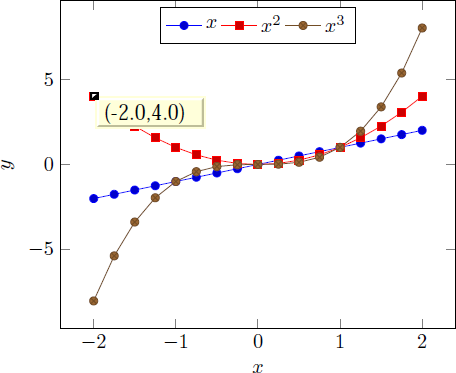
\includegraphics[height=6cm]{figures/pgfplotsclickable-fig1.png}
    \rlap{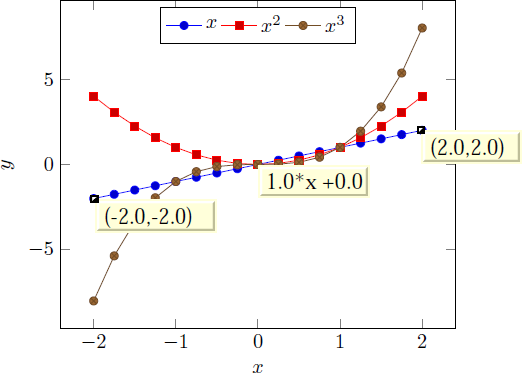
\includegraphics[height=6cm]{figures/pgfplotsclickable-fig2.png}}\hfill

\nobreak 这些截图展示了点击坐标轴范围（左列）以及从一点拖动到另一点（右列）的
结果。第二种情况展示了拖放的结果：它显示起点与终点，以及从拖动第一点到释放鼠标
第二点之间线段的方程。该线段为
%
    \[ l(x; x_0,y_0,x_1,y_1) = m \cdot x + n \]
%
其中 $m = (y_1-y_0) / (x_1-x_0)$ 为斜率，$n$ 为偏移量，其选取使得
$l(x_0;\dotsc) = y_0$。对于对数坐标图，会在计算斜率之前先取对数。

    \noindent
    \hbox to \linewidth{%
    \hspace{-0.5cm}%
    \begin{tikzpicture}
        \node at (8cm,0cm)    {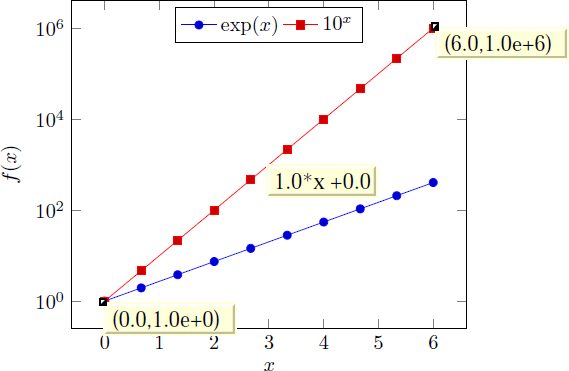
\includegraphics[height=6cm]{figures/pgfplotsclickable-fig4.png}};
        \node at (0cm,0cm)    {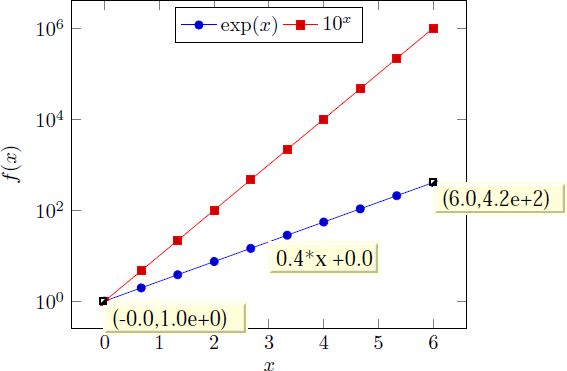
\includegraphics[height=6cm]{figures/pgfplotsclickable-fig3.png}};
    \end{tikzpicture}\hss}%

\nobreak 这些截图展示了\emph{对数}坐标轴下拖放的结果：端点再次显示坐标（不取对数），
中间的表单字段显示对数坐标下线性方程的斜率与偏移。

任何对数坐标轴的对数底通常为~$10$，但它会遵循 |log basis x| 与 |log basis y| 的
当前设置。所使用的对数与坐标轴描述所用的对数一致（这\emph{不一定}与
\PGFPlotstable{} 所用的相同！）。

本文档使用 |clickable| 库生成，因此可以在 Acrobat Reader 中打开它，直接点击图。

    \expandafter\ifx\csname pgfplotsclickabledisabled\endcsname\relax
    \else
    \paragraph{注意：}
    对于本文档，|clickable| 库已被禁用。你可以在
    \url{https://github.com/pgf-tikz/pgfplots} 上找到不同的版本。
    \fi

\begin{pgfplotskey}{clickable coords=\marg{displayed text}}
    点击绘图坐标时启用“吸附到最近点”特性。\meta{displayed text} 默认显示坐标的
    $x$ 与 $y$ 值（即你只需写 |clickable coords|，不带等号）。
    %
\begin{codeexample}[]
\begin{tikzpicture}
\begin{loglogaxis}[
    clickable coords={
        Level \thisrow{level} (q=\thisrow{q})
    },
]
    \addplot table [x=dof,y=error] {
        level  dof      error           q
        1      4        2.50000000e-01  48
        2      16       6.25000000e-02  25
        3      64       1.56250000e-02  41
        4      256      3.90625000e-03  8
        5      1024     9.76562500e-04  22
        6      4096     2.44140625e-04  46
        7      16384    6.10351562e-05  40
        8      65536    1.52587891e-05  3
        9      262144   3.81469727e-06  1
        10     1048576  9.53674316e-07  9
    };
\end{loglogaxis}
\end{tikzpicture}
\end{codeexample}
    %
    \noindent 现在，点击数据点会显示 `Level 7 (q=40)'，而点击数据点之外的地方
    则与之前一样显示点击坐标：

        \noindent\hbox to \linewidth{\hfill
        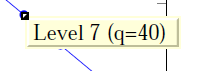
\includegraphics[scale=0.4]{figures/pgfplotsclickable-log-snap0}\hfill
        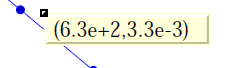
\includegraphics[scale=0.4]{figures/pgfplotsclickable-log-snap2}\hfill
        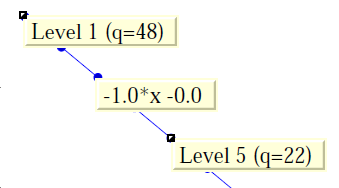
\includegraphics[scale=0.4]{figures/pgfplotsclickable-log-snap1}.\hfill
        }%

    注意，对数斜率的工作方式与之前相同。

    若希望显示 $(x,y)$ 值，请在 \meta{displayed text} 中使用特殊占位符
    `|(xy)|'。作为示例，再次考虑第~\pageref{pgfplots:scatterclasses} 页上的
    |scatter/classes| 例子：
    %
\begin{codeexample}[]
\begin{tikzpicture}
\begin{axis}[
    clickable coords={(xy): \thisrow{label}},
    scatter/classes={
        a={mark=square*,blue},
        b={mark=triangle*,red},
        c={mark=o,draw=black}   % <-- don't add comma
    }
]
    \addplot [
        only marks,
        scatter,
        scatter src=explicit symbolic
    ] table [meta=label] {
        x     y      label
        0.1   0.15   a
        0.45  0.27   c
        0.02  0.17   a
        0.06  0.1    a
        0.9   0.5    b
        0.5   0.3    c
        0.85  0.52   b
        0.12  0.05   a
        0.73  0.45   b
        0.53  0.25   c
        0.76  0.5    b
        0.55  0.32   c
    };
\end{axis}
\end{tikzpicture}
\end{codeexample}
    %
    \noindent 这里会看到类似如下的弹窗：

        \noindent\hbox to \linewidth{\hfill
        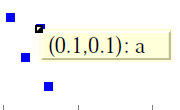
\includegraphics[scale=0.4]{figures/pgfplotsclickable-scatter1.png}\hfill
        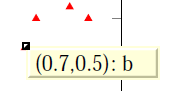
\includegraphics[scale=0.4]{figures/pgfplotsclickable-scatter2.png}\hfill
        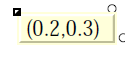
\includegraphics[scale=0.4]{figures/pgfplotsclickable-scatter0.png}.\hfill
        }%

    \meta{displayed text} 是一段富文本字符串，通过\emph{JavaScript}显示。
    对于大多数用途，它像未格式化的 C 字符串一样使用：包含字符，可能用 `|\n|'
    表示换行，或用 `|\t|' 表示制表符，但不应包含 \TeX{} 排版指令，尤其是数学模式
    （`|(xy)|' 替换文本由 |sprintf| 格式化，见下文）。若希望在显示前预处理数据，
    请考虑 |clickable coords code|。若遇到特殊字符问题，请尝试在其前面加反斜杠。
    若仍不行，尝试在单词前加 `|\\|' 和/或 `|\string|'。若要处理多行字段且需要
    调整大小分配，请考虑 |clickable coords size|。

    实际上，\meta{displayed text} 甚至可以包含富文本（即 XHTML）排版指令，如
    `|<br/>|'（注意末尾斜杠）或
    `|<span style="color:\#7E0000;">text</span>|'（注意 `|#|' 前的反斜杠），
    后者会改变 |text| 的颜色。|<span style="">| 的参数是 CSS 字段，CSS 属性列表
    请参考 HTML 文档。

    可以将 |clickable coords| 与三维坐标轴一起使用。注意，若三维坐标轴未设置
    |clickable coords|，其动态（可点击）特性将被禁用（因为它们似乎没用）。
    此外，三维坐标轴不支持斜率计算；只有“吸附到最近点”特性可用。

    可考虑使用 |annot/snap dist=6| 来增大“吸附到最近点”的距离。

    |clickable coords| 可以像上面的例子那样为坐标轴中的所有图指定，也可以为每个
    |\addplot| 命令分别指定（当希望对该命令使用“吸附到最近点”特性，并使用不同的
    \meta{displayed text} 时）。

    若多个 |clickable coords| 位于同一位置，每次点击会按出现顺序选择下一个。
\end{pgfplotskey}

\begin{pgfplotskey}{clickable coords code=\marg{%
    \TeX{} code which defines {\normalfont\ttfamily\textbackslash pgfplotsretval}}%
}
    这是 |clickable coords| 的一个变体，允许在将显示信息交给 JavaScript 之前
    对其进行预处理。

    该值应为 \TeX{} 代码，以某种方式定义 |\pgfplotsretval|。结果用作与坐标关联的
    简单未格式化字符串。

    可考虑使用

    \hspace{2em}|\pgfmathprintnumberto[verbatim]|\marg{number}|\macroname|

    \hspace{2em}|\edef\pgfplotsretval{Number=\macroname}|

    来提供数字打印。|\pgfmathprintnumberto[verbatim]| 不使用数学模式格式化
    数字，\footnote{数字打印的细节见 \PGFPlotstable{} 手册。}
    并将结果写入 |\macroname|。名称 `|\macroname|' 是任意的，可使用
    `|\eps|' 或 `|\info|' 之类。|\edef| 表示“展开定义”，其效果是展开所有宏以
    确定值，在本例中即“Number = \meta{the value}”。下面的例子使用它两次来美观地
    打印数据：
    %
\begin{codeexample}[]
\begin{tikzpicture}
\begin{loglogaxis}[clickable coords code={
    \pgfmathprintnumberto[verbatim,precision=1]
        {\thisrow{error}}
        \error
    \pgfmathprintnumberto[verbatim,frac]
        {\thisrow{frac}}
        \fraccomp
    \edef\pgfplotsretval{error \error, R=\fraccomp}
}]
    \addplot table [x=dof,y=error] {
        level  dof     error           frac
        1      4       2.50000000e-01  0.5
        2      16      6.25000000e-02  0.75
        3      64      1.56250000e-02  0.1
        4      256     3.90625000e-03  0.2
        5      1024    9.76562500e-04  0.5
        6      4096    2.44140625e-04  0.8
        7      16384   6.10351562e-05  0.125
        8      65536   1.52587891e-05  0.725
        9      262144  3.81469727e-06  0.625
        10     1048576 9.53674316e-07  1
    };
\end{loglogaxis}
\end{tikzpicture}
\end{codeexample}
    %
    \noindent 结果为

        \noindent\hbox to \linewidth{\hfill
        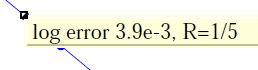
\includegraphics[scale=0.4]{figures/pgfplotsclickable-logcode-snap0.png}\hfill
        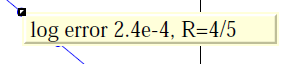
\includegraphics[scale=0.4]{figures/pgfplotsclickable-logcode-snap1.png}.\hfill
        }%

    \meta{\TeX{} code} 在局部作用域内求值，之后所有局部声明的变量都会被释放
    （因此可以使用任意名称）。
\end{pgfplotskey}

\begin{pgfplotskey}{%
    clickable coords size=\texttt{auto} or \marg{max chars} or
    \marg{max chars x,max chars y} (initially auto)%
}
    这实际上就是 |annot/popup size snap| 的另一个名称，见下文其文档。
\end{pgfplotskey}


\subsection{库的要求}

\begin{itemize}
    \item 本库依赖 \LaTeX{} 宏包 |insdljs|（“Insert document level JavaScript”）
        与 |eforms|，二者均属于免费的 |AcroTeX| 教育套件~\cite{acrotex}。
        \footnote{这些宏包依赖 \LaTeX{}，因此本库仅适用于 \LaTeX{}，
        不适用于 plain \TeX{} 或 Con\TeX{}t。}
        |insdljs| 宏包会创建一个扩展名为 |.djs| 的临时文件。
    \item 在撰写本文时，只有 Adobe Acrobat Reader 能正确解释 JavaScript 与表单。
        据我所知，若生成的文档在其他阅读器中使用，本库不会产生任何效果。
\end{itemize}
%
注意，虽然本库是为 \PGFPlots{} 编写的，但它可以独立于 \PGFPlots{} 环境使用。


\paragraph{兼容性问题：}

使用本库时有若干限制。其中大部分将在未来版本中消失——但到目前为止，我无法
施展魔法。
%
\begin{itemize}
    \item 本库尚不支持旋转坐标轴。对这些坐标轴请使用 |clickable=false|。
    \item 本库仅适用于 |pdflatex|；不支持 |dvips| 或 |dvipdfm|。
        \footnote{实际上它们应该可以支持。我并不确知为何不行。欢迎提供线索。}
    \item 到目前为止，\emph{无法}将本库与 |external| 库及第~\ref{cha:pgfplots:importexport}
        章中的其他图像外部化方法一起使用。

        更准确地说，你可以（通过两行额外导言代码，见下）得到正确标注、导出的
        \pdf{} 文档，但 |\includegraphics| 命令不会导入动态特性。

        若决定使用此变通方法，需要在加载 \pgfname{}、\Tikz{} 或 \PGFPlots{}
        \emph{之前}插入
        %
\begin{codeexample}[code only]
% \maxdeadcycles=10000 % in case you get the error `Output loop---<N> consecutive dead cycles.'
\usepackage[pdftex]{eforms}
\end{codeexample}
        %
        \noindent。|\maxdeadcycles| 对于大型文档似乎是必要的，请尝试一下。

        在编写文档草稿期间，你可能希望在导言区使用
        %
\begin{codeexample}[code only]
\pgfkeys{/pgf/images/include external/.code={\href{file:#1}{\pgfimage{#1}}}}
\end{codeexample}
        %
        这会在图形文件周围生成超链接，链接到导出的图片。点击超链接会打开导出的
        图片，而该图片本身是用 |clickable| 库生成的，因而支持动态特性。
        \footnote{这种特殊处理要求外部文件与主文档位于同一基目录，因此这种方法
        \emph{肯定}不适用于最终文档。}
    \item 本库会在 |\begin{document}| 处自动调用 |\begin{Form}|，并在文档末尾调用
        |\end{Form}|。hyperref 的该环境对于动态用户交互是必要的，若文档包含其他
        表单元素，请记住这一点。
\end{itemize}

\paragraph{致谢：}

\begin{itemize}
    \item 我使用了 Kevin van Zonneveld 的 JavaScript |sprintf| 实现~\cite{phptojs}
        （JavaScript API 仅提供有限的转换集合）。
\end{itemize}


\subsection{自定义}

可以通过若干选项自定义本库。

\begin{pgfplotskey}{clickable=\mchoice{true,false} (initially true)}
    允许对单个图禁用本库。
\end{pgfplotskey}

\begin{pgfplotskey}{annot/js fillColor=\marg{JavaScript color} (initially ["RGB",1,1,.855])}
    设置短弹窗注释的背景（填充）颜色。

    可选值为 |transparent|、灰色、RGB 或 CMYK 颜色，以四元素数组形式指定，形如
    |["RGB", |\meta{red}|,|\meta{green}|,|\meta{blue}|]|。每个颜色分量介于
    $0$ 与 $1$ 之间。

    再次强调：该选项用于 JavaScript。\emph{不能}像在 \pgfname{} 中那样使用颜色。
\end{pgfplotskey}

\begin{pgfplotskeylist}{%
    annot/point format=\marg{sprintf-format} (initially {(\%.1f,\%.1f)}),
    annot/point format 3d=\marg{sprintf-format} (initially {(\%.1f,\%.1f,\%.1f)})%
}
    允许提供 |sprintf| 格式字符串，用于填充注释文本。|sprintf| 的第一个参数为
    $x$ 坐标，第二个参数为 $y$ 坐标。

    |point format 3d| 变体用于任何三维坐标轴，而 |point format|（仅）用于二维坐标轴。

    |every semilogx axis|、|every semilogy axis| 与 |every loglog axis| 样式已更新为
    %
\begin{codeexample}[code only]
\pgfplotsset{
    every semilogy axis/.append style={/pgfplots/annot/point format={(\%.1f,\%.1e)}},
    every semilogx axis/.append style={/pgfplots/annot/point format={(\%.1e,\%.1f)}},
    every loglog axis/.append style={/pgfplots/annot/point format={(\%.1e,\%.1e)}},
}
\end{codeexample}
    %
    \noindent 从而每个对数坐标都以科学计数法显示。
\end{pgfplotskeylist}

\begin{pgfplotskey}{annot/slope format=\marg{sprintf-format} (initially \%.1f*x \%+.1f)}
    允许提供 |sprintf| 格式字符串，用于填充斜率注释文本。第一个参数为斜率，
    第二个为直线偏移。
\end{pgfplotskey}

\begin{pgfplotskey}{annot/printable=\mchoice{true,false} (initially false)}
    用于配置是否打印小注释。否则它们仅在屏幕上可见。
\end{pgfplotskey}

\begin{pgfplotskey}{annot/font=\marg{JavaScript font name} (initially font.Times)}
    用于为注释选择 JavaScript 字体。可选项限于 JavaScript 所接受的范围
    （\emph{不}与 \LaTeX{} 相同）。默认字体及其名称如下所示。

    \begin{center}
        \begin{tabular}{ll}
                \toprule
            字体名称             & JavaScript 中的名称 \\
                \midrule
            Times-Roman           & font.Times         \\
            Times-Bold            & font.TimesB        \\
            Times-Italic          & font.TimesI        \\
            Times-BoldItalic      & font.TimesBI       \\
            Helvetica             & font.Helv          \\
            Helvetica-Bold        & font.HelvB         \\
            Helvetica-Oblique     & font.HelvI         \\
            Helvetica-BoldOblique & font.HelvBI        \\
            Courier               & font.Cour          \\
            Courier-Bold          & font.CourB         \\
            Courier-Oblique       & font.CourI         \\
            Courier-BoldOblique   & font.CourBI        \\
            Symbol                & font.Symbol        \\
            ZapfDingbats          & font.ZapfD         \\
                \bottomrule
        \end{tabular}
    \end{center}
\end{pgfplotskey}

\begin{pgfplotskey}{annot/textSize=\marg{Size in Point} (initially 11)}
    设置注释的文字大小，单位为磅。
\end{pgfplotskey}

\begin{pgfplotskeylist}{%
    annot/popup size generic=\texttt{auto} or \marg{x} or \marg{x,y} (initially auto),
    annot/popup size snap=\texttt{auto} or \marg{x} or \marg{x,y} (initially auto),
    annot/popup size=\marg{value}%
}
    第一个键定义仅点击坐标轴时弹窗的大小。第二个键定义“吸附到最近点”特性
    （即由 |clickable coords| 准备的那些）的弹窗大小。第三个键将二者设为相同的
    \meta{value}。

    参数可以为 |auto|，此时 \PGFPlots{} 会尝试智能地统计字符数。这对多行文本
    可能失败。选项 \meta{x} 仅提供\emph{水平}大小，单位为 |annot/textSize|。
    因此，|annot/popup size generic=6| 使弹窗宽为 $6\cdot 11$ 磅。此时只分配一行。
    最后，\meta{x,y} 允许提供水平与竖直大小，均以 |annot/textSize| 为单位。

    另见 |clickable coords size|，它是 |annot/popup size snap| 的别名。
\end{pgfplotskeylist}

\begin{pgfplotskey}{annot/snap dist=\marg{Size in Point} (initially 4)}
    定义两次鼠标点击被视为等价的距离，以磅为单位（欧氏距离）。
\end{pgfplotskey}

\begin{pgfplotskey}{annot/richtext=\mchoice{true,false} (initially true)}
    启用或禁用 |clickable coords| 参数中的富文本排版。富文本类似于 XHTML，
    允许使用 CSS 样式，如颜色、字体变化及其他 CSS 属性，细节见 |clickable coords|
    文档。

    |annot/richtext=false| 的情况可能更稳健。
\end{pgfplotskey}


\subsection{在其他场合使用可点击库}

本库本质上提供一个命令 |\pgfplotsclickablecreate|，它创建一个预定义大小的可点击
区域，并结合 JavaScript 交互代码。它可以独立于 \PGFPlots{} 使用。

\begin{command}{\pgfplotsclickablecreate\oarg{required key-value-options}}
    创建一个可点击区域。点击会产生一个弹窗，其中包含光标所在点的信息。

    完整（！）的上下文需要通过键值对提供，既可以在调用本方法之前设置，也可以在
    \oarg{required key-value-options} 内设置。

    该命令实际上创建一个 AcroForm，点击时调用 JavaScript。它会创建一个表示上下文
    （坐标轴范围与选项）的 JavaScript 对象。该 JavaScript 对象在运行时可用。

    本方法是公开的，\emph{不}限于 \PGFPlots{} 使用。\PGFPlots{} 的钩子只是初始化
    所需的键值对。

    本方法不绘制任何内容。它仅初始化可点击区域与 JavaScript 代码。

    所需的键值对见下文文档。

    \paragraph{注意：}

    这里\emph{不会}执行完整的键值校验。可能出现无效选项在 Acrobat Reader 中打开时
    产生 JavaScript 错误。请使用 JavaScript 控制台查找它们。
\end{command}

\noindent 以下所有选项仅对希望在不使用 \PGFPlots{} 的情况下使用本库的用户有意义。

\begin{pgfplotskey}{annot/width=\marg{dimension} (initially -)}
    该必需键将区域宽度传达给 |\pgfplotsclickablecreate|。它必须是 \TeX{} 尺寸，
    如 |5cm|。
\end{pgfplotskey}

\begin{pgfplotskey}{annot/height=\marg{dimension} (initially -)}
    该必需键将区域高度传达给 |\pgfplotsclickablecreate|。它必须是 \TeX{} 尺寸，
    如 |5cm|。
\end{pgfplotskey}

\begin{pgfplotskey}{annot/jsname=\marg{string} (initially -)}
    该必需键将唯一标识符传达给 |\pgfplotsclickablecreate|。该标识符用于在
    JavaScript 中标识对象，因此不能有多个。若为空，将生成默认标识符。
\end{pgfplotskey}

\begin{pgfplotskeylist}{%
    annot/xmin=\marg{number},
    annot/xmax=\marg{number},
    annot/ymin=\marg{number},
    annot/ymax=\marg{number} (initially empty)%
}
    这些必需键将坐标轴范围传达给 |\pgfplotsclickablecreate|。它们应设置为
    可赋值给 JavaScript 浮点数（标准 IEEE 双精度）的数字。
\end{pgfplotskeylist}

\begin{pgfplotskey}{annot/collected plots=\marg{nested arrays} (initially empty)}
    实现“吸附到最近点”特性的底层接口。其值为图的数组，每个图又是坐标的数组，
    而每个坐标是 $x$、$y$ 与文本三个元素的数组。细节与示例请参考代码注释。
\end{pgfplotskey}
\endgroup


\begingroup
\tikzset{external/figure name/.add={}{brewer_}}%
    \tikzset{
%        font=\scriptsize,
        matrix style/.style={
            font=\tiny,
            every matrix/.append style={
                matrix anchor=north,
                inner ysep=0pt,
%                fill=red!10,
                ampersand replacement=\&,
                matrix of nodes,
                nodes={
                    anchor=south,
                    minimum size=2mm,
                },
                row 1/.style={
                    inner sep=0pt,
                },
                column 1/.style={
                    inner ysep=0pt,
                    anchor=base east,
                },
                row 2 column 1/.style={
                    every node/.append style={
                        font=\bfseries\scriptsize,
%                        font=\bfseries\tiny,
                        draw,
                    },
                },
                row sep=0pt,
                column sep=0pt,
            },
        },
    }


% =============================================================================
%\def\MATRIXseq#1{%
\NewDocumentCommand{\MATRIXseq}{sm}{{%
\tikzset{/tikz/external/export=true}%
\newcommand*\scheme{#2}%
\pgfmanualpdflabel{colormap/\scheme-3}{}%
\pgfmanualpdflabel{colormap/\scheme-4}{}%
\pgfmanualpdflabel{colormap/\scheme-5}{}%
\pgfmanualpdflabel{colormap/\scheme-6}{}%
\pgfmanualpdflabel{colormap/\scheme-7}{}%
\pgfmanualpdflabel{colormap/\scheme-8}{}%
\pgfmanualpdflabel{colormap/\scheme-9}{}%
\pgfmanualpdflabel{colormap/\scheme}{}%
\foreach \x in {A,...,M} {\pgfmanualpdflabel{\scheme-\x}{}}%
\tikzsetnextfilename{brewer-seq-#2}%
\begin{tikzpicture}[
    matrix style,
]
    % instantiate all colormaps for \scheme:
    \pgfplotsset{
        colormap/\scheme-3,
        colormap/\scheme-4,
        colormap/\scheme-5,
        colormap/\scheme-6,
        colormap/\scheme-7,
        colormap/\scheme-8,
        colormap/\scheme-9,
        colormap/\scheme,
    }%
    %
    % directly access the correct color:
    % #1 is one of A,B,...,M
    \def\C##1{\node [fill=\scheme-##1] {};}%
    % in case the color should be white, also draw a black frame
    \def\D##1{\node [draw=black,fill=\scheme-##1] {};}%
    %
    % indirectly access the correct color
    % #1 is an index into the colormap, 0,1,...,13
    % #2 is the number of colors in the colormap (qualifies which colormap to use)
    % This is redundant, but it allows us to verify that the colormaps
    % work as intended without typos:
    \newcommand*\CC[2]{\node [/pgfplots/index of colormap=##1 of \scheme-##2, fill] {};}%
    % in case the color should be white, also draw a black frame
    \newcommand*\DD[2]{\node [/pgfplots/index of colormap=##1 of \scheme-##2, fill, draw=black] {};}%
    %
    % define a colorbar that has the same size as a row of colors in the matrix
    \newcommand*\CM{%
        \node[inner sep=0pt,xshift=-3.5pt,overlay,anchor=south west]{%
\IfBooleanTF{#1}{%
            \pgfmathparse{14*2mm + 16*\pgflinewidth + 1.0pt}%
}{%
            \pgfmathparse{14*2mm + 15*\pgflinewidth + 1.1pt}%
}
            \let\width=\pgfmathresult
            \pgfplotscolormaptoshadingspec{\scheme}{\width pt}\result
            \def\tempb{\pgfdeclarehorizontalshading{tempshading}{2mm}}%
            \expandafter\tempb\expandafter{\result}%
            \pgfuseshading{tempshading}%
        };
    }%
    \matrix {
\IfBooleanTF{#1}{%
                \& A         \& B         \& C         \& D         \& E         \& F         \& G         \& H         \& I         \& J         \& K         \& L         \& M         \\
        \scheme \& \D{A}     \& \C{B}     \& \C{C}     \& \C{D}     \& \C{E}     \& \C{F}     \& \C{G}     \& \C{H}     \& \C{I}     \& \C{J}     \& \C{K}     \& \C{L}     \& \C{M}     \\
        3       \&           \&           \& \CC{0}{3} \&           \&           \& \CC{1}{3} \&           \&           \& \CC{2}{3} \&           \&           \&           \&           \\
        4       \&           \& \CC{0}{4} \&           \&           \& \CC{1}{4} \&           \& \CC{2}{4} \&           \&           \& \CC{3}{4} \&           \&           \&           \\
        5       \&           \& \CC{0}{5} \&           \&           \& \CC{1}{5} \&           \& \CC{2}{5} \&           \& \CC{3}{5} \&           \& \CC{4}{5} \&           \&           \\
        6       \&           \& \CC{0}{6} \&           \& \CC{1}{6} \&           \& \CC{2}{6} \& \CC{3}{6} \&           \& \CC{4}{6} \&           \& \CC{5}{6} \&           \&           \\
        7       \&           \& \CC{0}{7} \&           \& \CC{1}{7} \&           \& \CC{2}{7} \& \CC{3}{7} \& \CC{4}{7} \&           \& \CC{5}{7} \&           \& \CC{6}{7} \&           \\
        8       \& \DD{0}{8} \&           \& \CC{1}{8} \& \CC{2}{8} \&           \& \CC{3}{8} \& \CC{4}{8} \& \CC{5}{8} \&           \& \CC{6}{8} \&           \& \CC{7}{8} \&           \\
        9       \& \DD{0}{9} \&           \& \CC{1}{9} \& \CC{2}{9} \&           \& \CC{3}{9} \& \CC{4}{9} \& \CC{5}{9} \&           \& \CC{6}{9} \& \CC{7}{9} \&           \& \CC{8}{9} \\
        CM      \& \CM       \&           \&           \&           \&           \&           \&           \&           \&           \&           \&           \&           \&           \\
%                \& A         \& B         \& C         \& D         \& E         \& F         \& G         \& H         \& I         \& J         \& K         \& L         \& M         \\
%                \& \D{A}     \& \C{B}     \& \C{C}     \& \C{D}     \& \C{E}     \& \C{F}     \& \C{G}     \& \C{H}     \& \C{I}     \& \C{J}     \& \C{K}     \& \C{L}     \& \C{M}     \\
%                \&           \&           \& \CC{0}{3} \&           \&           \& \CC{1}{3} \&           \&           \& \CC{2}{3} \&           \&           \&           \&           \\
%                \&           \& \CC{0}{4} \&           \&           \& \CC{1}{4} \&           \& \CC{2}{4} \&           \&           \& \CC{3}{4} \&           \&           \&           \\
%                \&           \& \CC{0}{5} \&           \&           \& \CC{1}{5} \&           \& \CC{2}{5} \&           \& \CC{3}{5} \&           \& \CC{4}{5} \&           \&           \\
%                \&           \& \CC{0}{6} \&           \& \CC{1}{6} \&           \& \CC{2}{6} \& \CC{3}{6} \&           \& \CC{4}{6} \&           \& \CC{5}{6} \&           \&           \\
%                \&           \& \CC{0}{7} \&           \& \CC{1}{7} \&           \& \CC{2}{7} \& \CC{3}{7} \& \CC{4}{7} \&           \& \CC{5}{7} \&           \& \CC{6}{7} \&           \\
%                \& \DD{0}{8} \&           \& \CC{1}{8} \& \CC{2}{8} \&           \& \CC{3}{8} \& \CC{4}{8} \& \CC{5}{8} \&           \& \CC{6}{8} \&           \& \CC{7}{8} \&           \\
%                \& \DD{0}{9} \&           \& \CC{1}{9} \& \CC{2}{9} \&           \& \CC{3}{9} \& \CC{4}{9} \& \CC{5}{9} \&           \& \CC{6}{9} \& \CC{7}{9} \&           \& \CC{8}{9} \\
}{%
                \& A         \& B         \& C         \& D         \& E         \& F         \& G         \& H         \& I         \& J         \& K         \& L         \& M         \\
        \scheme \& \C{A}     \& \C{B}     \& \C{C}     \& \C{D}     \& \C{E}     \& \C{F}     \& \C{G}     \& \C{H}     \& \C{I}     \& \C{J}     \& \C{K}     \& \C{L}     \& \C{M}     \\
        3       \&           \&           \& \CC{0}{3} \&           \&           \& \CC{1}{3} \&           \&           \& \CC{2}{3} \&           \&           \&           \&           \\
        4       \&           \& \CC{0}{4} \&           \&           \& \CC{1}{4} \&           \& \CC{2}{4} \&           \&           \& \CC{3}{4} \&           \&           \&           \\
        5       \&           \& \CC{0}{5} \&           \&           \& \CC{1}{5} \&           \& \CC{2}{5} \&           \& \CC{3}{5} \&           \& \CC{4}{5} \&           \&           \\
        6       \&           \& \CC{0}{6} \&           \& \CC{1}{6} \&           \& \CC{2}{6} \& \CC{3}{6} \&           \& \CC{4}{6} \&           \& \CC{5}{6} \&           \&           \\
        7       \&           \& \CC{0}{7} \&           \& \CC{1}{7} \&           \& \CC{2}{7} \& \CC{3}{7} \& \CC{4}{7} \&           \& \CC{5}{7} \&           \& \CC{6}{7} \&           \\
        8       \& \CC{0}{8} \&           \& \CC{1}{8} \& \CC{2}{8} \&           \& \CC{3}{8} \& \CC{4}{8} \& \CC{5}{8} \&           \& \CC{6}{8} \&           \& \CC{7}{8} \&           \\
        9       \& \CC{0}{9} \&           \& \CC{1}{9} \& \CC{2}{9} \&           \& \CC{3}{9} \& \CC{4}{9} \& \CC{5}{9} \&           \& \CC{6}{9} \& \CC{7}{9} \&           \& \CC{8}{9} \\
        CM      \& \CM       \&           \&           \&           \&           \&           \&           \&           \&           \&           \&           \&           \&           \\
%                \& A         \& B         \& C         \& D         \& E         \& F         \& G         \& H         \& I         \& J         \& K         \& L         \& M         \\
%                \& \C{A}     \& \C{B}     \& \C{C}     \& \C{D}     \& \C{E}     \& \C{F}     \& \C{G}     \& \C{H}     \& \C{I}     \& \C{J}     \& \C{K}     \& \C{L}     \& \C{M}     \\
%                \&           \&           \& \CC{0}{3} \&           \&           \& \CC{1}{3} \&           \&           \& \CC{2}{3} \&           \&           \&           \&           \\
%                \&           \& \CC{0}{4} \&           \&           \& \CC{1}{4} \&           \& \CC{2}{4} \&           \&           \& \CC{3}{4} \&           \&           \&           \\
%                \&           \& \CC{0}{5} \&           \&           \& \CC{1}{5} \&           \& \CC{2}{5} \&           \& \CC{3}{5} \&           \& \CC{4}{5} \&           \&           \\
%                \&           \& \CC{0}{6} \&           \& \CC{1}{6} \&           \& \CC{2}{6} \& \CC{3}{6} \&           \& \CC{4}{6} \&           \& \CC{5}{6} \&           \&           \\
%                \&           \& \CC{0}{7} \&           \& \CC{1}{7} \&           \& \CC{2}{7} \& \CC{3}{7} \& \CC{4}{7} \&           \& \CC{5}{7} \&           \& \CC{6}{7} \&           \\
%                \& \CC{0}{8} \&           \& \CC{1}{8} \& \CC{2}{8} \&           \& \CC{3}{8} \& \CC{4}{8} \& \CC{5}{8} \&           \& \CC{6}{8} \&           \& \CC{7}{8} \&           \\
%                \& \CC{0}{9} \&           \& \CC{1}{9} \& \CC{2}{9} \&           \& \CC{3}{9} \& \CC{4}{9} \& \CC{5}{9} \&           \& \CC{6}{9} \& \CC{7}{9} \&           \& \CC{8}{9} \\
}
    };
\end{tikzpicture}%
}}

\NewDocumentCommand{\MATRIXdiv}{sm}{{%
\newcommand*\scheme{#2}%
\tikzset{/tikz/external/export=true}%
\pgfmanualpdflabel{colormap/\scheme-3}{}%
\pgfmanualpdflabel{colormap/\scheme-4}{}%
\pgfmanualpdflabel{colormap/\scheme-5}{}%
\pgfmanualpdflabel{colormap/\scheme-6}{}%
\pgfmanualpdflabel{colormap/\scheme-7}{}%
\pgfmanualpdflabel{colormap/\scheme-8}{}%
\pgfmanualpdflabel{colormap/\scheme-9}{}%
\pgfmanualpdflabel{colormap/\scheme-10}{}%
\pgfmanualpdflabel{colormap/\scheme-11}{}%
\pgfmanualpdflabel{colormap/\scheme}{}%
\foreach \x in {A,...,O} {\pgfmanualpdflabel{\scheme-\x}{}}%
\tikzsetnextfilename{brewer-div-#2}%
\begin{tikzpicture}[
    matrix style,
]
    % instantiate all colormaps for \scheme:
    \pgfplotsset{
        colormap/\scheme-3,
        colormap/\scheme-4,
        colormap/\scheme-5,
        colormap/\scheme-6,
        colormap/\scheme-7,
        colormap/\scheme-8,
        colormap/\scheme-9,
        colormap/\scheme-10,
        colormap/\scheme-11,
        colormap/\scheme,
    }%
    %
    % directly access the correct color:
    % #1 is one of A,B,...,M
    \def\C##1{\node [fill=\scheme-##1] {};}%
    % in case the color should be white, also draw a black frame
    \def\D##1{\node [draw=black,fill=\scheme-##1] {};}%
    %
    % indirectly access the correct color
    % #1 is an index into the colormap, 0,1,...,13
    % #2 is the number of colors in the colormap (qualifies which colormap to use)
    % This is redundant, but it allows us to verify that the colormaps
    % work as intended without typos:
    \newcommand*\CC[2]{\node [/pgfplots/index of colormap=##1 of \scheme-##2, fill] {};}%
    % in case the color should be white, also draw a black frame
    \newcommand*\DD[2]{\node [/pgfplots/index of colormap=##1 of \scheme-##2, fill, draw=black] {};}%
    %
    % define a colorbar that has the same size as a row of colors in the matrix
    \newcommand*\CM{%
        \node[inner sep=0pt,xshift=-3.5pt,overlay,anchor=south west]{%
\IfBooleanTF{#1}{%
            \pgfmathparse{16*2mm + 18*\pgflinewidth + 2.3pt}%
}{%
            \pgfmathparse{16*2mm + 17*\pgflinewidth + 2.3pt}%
}%
            \let\width=\pgfmathresult
            \pgfplotscolormaptoshadingspec{\scheme}{\width pt}\result
            \def\tempb{\pgfdeclarehorizontalshading{tempshading}{2mm}}%
            \expandafter\tempb\expandafter{\result}%
            \pgfuseshading{tempshading}%
        };
    }%
    \matrix {
\IfBooleanTF{#1}{%
                \& A          \& B          \& C         \& D          \& E         \& F          \& G          \& H          \& I          \& J          \& K         \& L          \& M         \& N          \& O           \\
        \scheme \& \C{A}      \& \C{B}      \& \C{C}     \& \C{D}      \& \C{E}     \& \C{F}      \& \C{G}      \& \D{H}      \& \C{I}      \& \C{J}      \& \C{K}     \& \C{L}      \& \C{M}     \& \C{N}      \& \C{O}       \\
        3       \&            \&            \&           \&            \& \CC{0}{3} \&            \&            \& \DD{1}{3}  \&            \&            \& \CC{2}{3} \&            \&           \&            \&             \\
        4       \&            \&            \& \CC{0}{4} \&            \&           \& \CC{1}{4}  \&            \&            \&            \& \CC{2}{4}  \&           \&            \& \CC{3}{4} \&            \&             \\
        5       \&            \&            \& \CC{0}{5} \&            \&           \& \CC{1}{5}  \&            \& \DD{2}{5}  \&            \& \CC{3}{5}  \&           \&            \& \CC{4}{5} \&            \&             \\
        6       \&            \& \CC{0}{6}  \&           \&            \& \CC{1}{7} \&            \& \CC{2}{6}  \&            \& \CC{3}{6}  \&            \& \CC{4}{6} \&            \&           \& \CC{5}{6}  \&             \\
        7       \&            \& \CC{0}{7}  \&           \&            \& \CC{1}{7} \&            \& \CC{2}{7}  \& \DD{3}{7}  \& \CC{4}{7}  \&            \& \CC{5}{7} \&            \&           \& \CC{6}{7}  \&             \\
        8       \&            \& \CC{0}{8}  \&           \& \CC{1}{8}  \&           \& \CC{2}{8}  \& \CC{3}{8}  \&            \& \CC{4}{8}  \& \CC{5}{8}  \&           \& \CC{6}{8}  \&           \& \CC{7}{8}  \&             \\
        9       \&            \& \CC{0}{9}  \&           \& \CC{1}{9}  \&           \& \CC{2}{9}  \& \CC{3}{9}  \& \DD{4}{9}  \& \CC{5}{9}  \& \CC{6}{9}  \&           \& \CC{7}{9}  \&           \& \CC{8}{9}  \&             \\
        10      \& \CC{0}{10} \& \CC{1}{10} \&           \& \CC{2}{10} \&           \& \CC{3}{10} \& \CC{4}{10} \&            \& \CC{5}{10} \& \CC{6}{10} \&           \& \CC{7}{10} \&           \& \CC{8}{10} \& \CC{9}{10}  \\
        11      \& \CC{0}{11} \& \CC{1}{11} \&           \& \CC{2}{11} \&           \& \CC{3}{11} \& \CC{4}{11} \& \DD{5}{11} \& \CC{6}{11} \& \CC{7}{11} \&           \& \CC{8}{11} \&           \& \CC{9}{11} \& \CC{10}{11} \\
        CM      \& \CM        \&            \&           \&            \&           \&            \&            \&            \&            \&            \&           \&            \&           \&            \&             \\
}{%
                \& A          \& B          \& C         \& D          \& E         \& F          \& G          \& H          \& I          \& J          \& K         \& L          \& M         \& N          \& O           \\
        \scheme \& \C{A}      \& \C{B}      \& \C{C}     \& \C{D}      \& \C{E}     \& \C{F}      \& \C{G}      \& \C{H}      \& \C{I}      \& \C{J}      \& \C{K}     \& \C{L}      \& \C{M}     \& \C{N}      \& \C{O}       \\
        3       \&            \&            \&           \&            \& \CC{0}{3} \&            \&            \& \CC{1}{3}  \&            \&            \& \CC{2}{3} \&            \&           \&            \&             \\
        4       \&            \&            \& \CC{0}{4} \&            \&           \& \CC{1}{4}  \&            \&            \&            \& \CC{2}{4}  \&           \&            \& \CC{3}{4} \&            \&             \\
        5       \&            \&            \& \CC{0}{5} \&            \&           \& \CC{1}{5}  \&            \& \CC{2}{5}  \&            \& \CC{3}{5}  \&           \&            \& \CC{4}{5} \&            \&             \\
        6       \&            \& \CC{0}{6}  \&           \&            \& \CC{1}{7} \&            \& \CC{2}{6}  \&            \& \CC{3}{6}  \&            \& \CC{4}{6} \&            \&           \& \CC{5}{6}  \&             \\
        7       \&            \& \CC{0}{7}  \&           \&            \& \CC{1}{7} \&            \& \CC{2}{7}  \& \CC{3}{7}  \& \CC{4}{7}  \&            \& \CC{5}{7} \&            \&           \& \CC{6}{7}  \&             \\
        8       \&            \& \CC{0}{8}  \&           \& \CC{1}{8}  \&           \& \CC{2}{8}  \& \CC{3}{8}  \&            \& \CC{4}{8}  \& \CC{5}{8}  \&           \& \CC{6}{8}  \&           \& \CC{7}{8}  \&             \\
        9       \&            \& \CC{0}{9}  \&           \& \CC{1}{9}  \&           \& \CC{2}{9}  \& \CC{3}{9}  \& \CC{4}{9}  \& \CC{5}{9}  \& \CC{6}{9}  \&           \& \CC{7}{9}  \&           \& \CC{8}{9}  \&             \\
        10      \& \CC{0}{10} \& \CC{1}{10} \&           \& \CC{2}{10} \&           \& \CC{3}{10} \& \CC{4}{10} \&            \& \CC{5}{10} \& \CC{6}{10} \&           \& \CC{7}{10} \&           \& \CC{8}{10} \& \CC{9}{10}  \\
        11      \& \CC{0}{11} \& \CC{1}{11} \&           \& \CC{2}{11} \&           \& \CC{3}{11} \& \CC{4}{11} \& \CC{5}{11} \& \CC{6}{11} \& \CC{7}{11} \&           \& \CC{8}{11} \&           \& \CC{9}{11} \& \CC{10}{11} \\
        CM      \& \CM        \&            \&           \&            \&           \&            \&            \&            \&            \&            \&           \&            \&           \&            \&             \\
}
    };
\end{tikzpicture}%
}}

\NewDocumentCommand{\MATRIXqual}{mmO{0}}{{%
\tikzset{/tikz/external/export=true}%
\newcommand*\scheme{#2}%
\pgfmanualpdflabel{colormap/\scheme-3}{}%
\pgfmanualpdflabel{colormap/\scheme-4}{}%
\pgfmanualpdflabel{colormap/\scheme-5}{}%
\pgfmanualpdflabel{colormap/\scheme-6}{}%
\pgfmanualpdflabel{colormap/\scheme-7}{}%
\pgfmanualpdflabel{colormap/\scheme-8}{}%
\ifnum#1>8
\pgfmanualpdflabel{colormap/\scheme-9}{}%
\ifnum#1>9
\pgfmanualpdflabel{colormap/\scheme-10}{}%
\pgfmanualpdflabel{colormap/\scheme-11}{}%
\pgfmanualpdflabel{colormap/\scheme-12}{}%
\fi
\fi
\pgfmanualpdflabel{colormap/\scheme}{}%
\tikzsetnextfilename{brewer-qualit-#2}%
\begin{tikzpicture}[
    baseline,
    matrix style,
]
    \newcommand*\classes{#1}%
    % instantiate all colormaps for \scheme:
    \pgfplotsset{
        colormap/\scheme-3,
        colormap/\scheme-4,
        colormap/\scheme-5,
        colormap/\scheme-6,
        colormap/\scheme-7,
        colormap/\scheme-8,
    }
\foreach \x in {A,...,H} {\pgfmanualpdflabel{\scheme-\x}{}}%
\ifnum\classes>8
\foreach \x in {I} {\pgfmanualpdflabel{\scheme-\x}{}}%
    \pgfplotsset{
        colormap/\scheme-9,
    }
\fi
\ifnum\classes=12
\foreach \x in {J,...,L} {\pgfmanualpdflabel{\scheme-\x}{}}%
    \pgfplotsset{
        colormap/\scheme-10,
        colormap/\scheme-11,
        colormap/\scheme-12,
    }
\fi
    \pgfplotsset{
        colormap/\scheme,
    }%
    %
    \newcommand*\EmptyRows{#3}

    % directly access the correct color:
    % #1 is one of A,B,...,M
    \def\C##1{\node [fill=\scheme-##1] {};}
    %
    % indirectly access the correct color
    % #1 is an index into the colormap, 0,1,...,13
    % #2 is the number of colors in the colormap (qualifies which colormap to use)
    % This is redundant, but it allows us to verify that the colormaps
    % work as intended without typos:
    \newcommand*\CC[2]{\node [/pgfplots/index of colormap=##1 of \scheme-##2, fill] {};}
    %
    % define dummy node to just produce space
    \newcommand*\Dummy{\node {};}
%    % define a colorbar that has the same size as a row of colors in the matrix
%\ifnum\classes=8
%    \newcommand*\CM{%
%        \node[inner sep=0pt,xshift=-3.5pt,overlay,anchor=south west]{%
%                \pgfmathparse{8*2mm + 8pt}%
%            \let\width=\pgfmathresult%
%            \pgfplotscolormaptoshadingspec{\scheme}{\width pt}\result%
%            \def\tempb{\pgfdeclarehorizontalshading{tempshading}{2mm}}%
%            \expandafter\tempb\expandafter{\result}%
%            \pgfuseshading{tempshading}%
%        };
%    }
%\else\ifnum\classes=9
%    \newcommand*\CM{%
%        \node[inner sep=0pt,xshift=-3.5pt,overlay,anchor=south west]{%
%                \pgfmathparse{9*2mm + 10*\pgflinewidth + 2.3pt}%
%            \let\width=\pgfmathresult%
%            \pgfplotscolormaptoshadingspec{\scheme}{\width pt}\result%
%            \def\tempb{\pgfdeclarehorizontalshading{tempshading}{2mm}}%
%            \expandafter\tempb\expandafter{\result}%
%            \pgfuseshading{tempshading}%
%        };
%    }
%\else\ifnum\classes=12
%    \newcommand*\CM{%
%        \node[inner sep=0pt,xshift=-3.5pt,overlay,anchor=south west]{%
%                \pgfmathparse{12*2mm + 13*\pgflinewidth + 2.3pt}%
%            \let\width=\pgfmathresult%
%            \pgfplotscolormaptoshadingspec{\scheme}{\width pt}\result%
%            \def\tempb{\pgfdeclarehorizontalshading{tempshading}{2mm}}%
%            \expandafter\tempb\expandafter{\result}%
%            \pgfuseshading{tempshading}%
%        };
%    }
%\fi\fi\fi
\ifnum\classes=8
    \matrix (m) {
                \& A          \& B          \& C          \& D          \& E          \& F          \& G          \& H          \\
        \scheme \& \C{A}      \& \C{B}      \& \C{C}      \& \C{D}      \& \C{E}      \& \C{F}      \& \C{G}      \& \C{H}      \\
        3       \& \CC{0}{3}  \& \CC{1}{3}  \& \CC{2}{3}  \&            \&            \&            \&            \&            \\
        4       \& \CC{0}{4}  \& \CC{1}{4}  \& \CC{2}{4}  \& \CC{3}{4}  \&            \&            \&            \&            \\
        5       \& \CC{0}{5}  \& \CC{1}{5}  \& \CC{2}{5}  \& \CC{3}{5}  \& \CC{4}{5}  \&            \&            \&            \\
        6       \& \CC{0}{6}  \& \CC{1}{6}  \& \CC{2}{6}  \& \CC{3}{6}  \& \CC{4}{6}  \& \CC{5}{6}  \&            \&            \\
        7       \& \CC{0}{7}  \& \CC{1}{7}  \& \CC{2}{7}  \& \CC{3}{7}  \& \CC{4}{7}  \& \CC{5}{7}  \& \CC{6}{7}  \&            \\
        8       \& \CC{0}{8}  \& \CC{1}{8}  \& \CC{2}{8}  \& \CC{3}{8}  \& \CC{4}{8}  \& \CC{5}{8}  \& \CC{6}{8}  \& \CC{7}{8}  \& \Dummy \& \Dummy \& \Dummy \& \Dummy \\
%%%%%        CM      \& \CM        \&            \&            \&            \&            \&            \&            \&            \\
    };
\else\ifnum\classes=9
    \matrix (m) {
                \& A          \& B          \& C          \& D          \& E          \& F          \& G          \& H          \& I         \\
        \scheme \& \C{A}      \& \C{B}      \& \C{C}      \& \C{D}      \& \C{E}      \& \C{F}      \& \C{G}      \& \C{H}      \& \C{I}     \\
        3       \& \CC{0}{3}  \& \CC{1}{3}  \& \CC{2}{3}  \&            \&            \&            \&            \&            \&           \\
        4       \& \CC{0}{4}  \& \CC{1}{4}  \& \CC{2}{4}  \& \CC{3}{4}  \&            \&            \&            \&            \&           \\
        5       \& \CC{0}{5}  \& \CC{1}{5}  \& \CC{2}{5}  \& \CC{3}{5}  \& \CC{4}{5}  \&            \&            \&            \&           \\
        6       \& \CC{0}{6}  \& \CC{1}{6}  \& \CC{2}{6}  \& \CC{3}{6}  \& \CC{4}{6}  \& \CC{5}{6}  \&            \&            \&           \\
        7       \& \CC{0}{7}  \& \CC{1}{7}  \& \CC{2}{7}  \& \CC{3}{7}  \& \CC{4}{7}  \& \CC{5}{7}  \& \CC{6}{7}  \&            \&           \\
        8       \& \CC{0}{8}  \& \CC{1}{8}  \& \CC{2}{8}  \& \CC{3}{8}  \& \CC{4}{8}  \& \CC{5}{8}  \& \CC{6}{8}  \& \CC{7}{8}  \&           \\
        9       \& \CC{0}{9}  \& \CC{1}{9}  \& \CC{2}{9}  \& \CC{3}{9}  \& \CC{4}{9}  \& \CC{5}{9}  \& \CC{6}{9}  \& \CC{7}{9}  \& \CC{8}{9} \& \Dummy \& \Dummy \& \Dummy \\
%%%%%        CM      \& \CM        \&            \&            \&            \&            \&            \&            \&            \&           \\
    };
\else\ifnum\classes=12
    \matrix (m) {
                \& A          \& B          \& C          \& D          \& E          \& F          \& G          \& H          \& I          \& J          \& K           \& L           \\
        \scheme \& \C{A}      \& \C{B}      \& \C{C}      \& \C{D}      \& \C{E}      \& \C{F}      \& \C{G}      \& \C{H}      \& \C{I}      \& \C{J}      \& \C{K}       \& \C{L}       \\
        3       \& \CC{0}{3}  \& \CC{1}{3}  \& \CC{2}{3}  \&            \&            \&            \&            \&            \&            \&            \&             \&             \\
        4       \& \CC{0}{4}  \& \CC{1}{4}  \& \CC{2}{4}  \& \CC{3}{4}  \&            \&            \&            \&            \&            \&            \&             \&             \\
        5       \& \CC{0}{5}  \& \CC{1}{5}  \& \CC{2}{5}  \& \CC{3}{5}  \& \CC{4}{5}  \&            \&            \&            \&            \&            \&             \&             \\
        6       \& \CC{0}{6}  \& \CC{1}{6}  \& \CC{2}{6}  \& \CC{3}{6}  \& \CC{4}{6}  \& \CC{5}{6}  \&            \&            \&            \&            \&             \&             \\
        7       \& \CC{0}{7}  \& \CC{1}{7}  \& \CC{2}{7}  \& \CC{3}{7}  \& \CC{4}{7}  \& \CC{5}{7}  \& \CC{6}{7}  \&            \&            \&            \&             \&             \\
        8       \& \CC{0}{8}  \& \CC{1}{8}  \& \CC{2}{8}  \& \CC{3}{8}  \& \CC{4}{8}  \& \CC{5}{8}  \& \CC{6}{8}  \& \CC{7}{8}  \&            \&            \&             \&             \\
        9       \& \CC{0}{9}  \& \CC{1}{9}  \& \CC{2}{9}  \& \CC{3}{9}  \& \CC{4}{9}  \& \CC{5}{9}  \& \CC{6}{9}  \& \CC{7}{9}  \& \CC{8}{9}  \&            \&             \&             \\
        10      \& \CC{0}{10} \& \CC{1}{10} \& \CC{2}{10} \& \CC{3}{10} \& \CC{4}{10} \& \CC{5}{10} \& \CC{6}{10} \& \CC{7}{10} \& \CC{8}{10} \& \CC{9}{10} \&             \&             \\
        11      \& \CC{0}{11} \& \CC{1}{11} \& \CC{2}{11} \& \CC{3}{11} \& \CC{4}{11} \& \CC{5}{11} \& \CC{6}{11} \& \CC{7}{11} \& \CC{8}{11} \& \CC{9}{11} \& \CC{10}{11} \&             \\
        12      \& \CC{0}{12} \& \CC{1}{12} \& \CC{2}{12} \& \CC{3}{12} \& \CC{4}{12} \& \CC{5}{12} \& \CC{6}{12} \& \CC{7}{12} \& \CC{8}{12} \& \CC{9}{12} \& \CC{10}{12} \& \CC{11}{12} \\
%%%%%        CM      \& \CM        \&            \&            \&            \&            \&            \&            \&            \&            \&            \&             \&             \\
    };
\fi\fi\fi

% insert space as fake empty rows
\ifnum\EmptyRows>0
    \path node [below=\EmptyRows*2mm of m,anchor=south] {};
\fi

\end{tikzpicture}%
}}

\section{ColorBrewer}
\def\pgfplotsmanualcurlibrary{colormaps}

{\emph{由 Vincent A.\ Traag 与 Stefan Pinnow 扩展}}

\begin{pgfplotslibrary}{colorbrewer}

本库将 Cynthia Brewer 创建、发布于
\url{http://colorbrewer2.org/} 的配色方案引入 PGFPlots。这些方案最初是为制图需求
设计的，但如今也用于其他类型的数据可视化。ColorBrewer 方案分为以下类型
%
\begin{description}
    \item[sequential] 适用于从低到高有序的数据；
    \item[diverging] 用于突出相对于某个均值的变化；
    \item[qualitative] 其中颜色没有特殊顺序。
\end{description}
%
每个方案最多可包含 12 个不同的数据类（即颜色），并同时以色图与循环列表的形式
提供。

{%
\centering

\pgfplotsset{
    brewer example/.style={
        small,
        title style={font=\normalfont},
    }
}%
\renewcommand{\arraystretch}{2}%
\tikzset{/tikz/external/export=true}%
\begin{tabular}{cc}
\begin{tikzpicture}[baseline]
    \begin{axis}[brewer example, hide axis,title={Diverging \texttt{colormap/PiYG-11}},colormap/PiYG-11,colorbar left]
        \addplot3[surf,
            domain=0:360,samples=40]
                {sin(x)*sin(y)};
    \end{axis}
\end{tikzpicture}
&
% ----- example in section 4.3 on page 43 -----
\tikzset{/tikz/external/export=true}%
\begin{tikzpicture}[baseline]
    % --- changed by Mo-Gul ---
    \begin{axis}[
        brewer example,
        hide axis,
        view={60}{30},
        title={Sequential \texttt{colormap/PuBu-9}},
        colormap/PuBu-9,
        colorbar right,
        clip bounding box=default tikz,
    ]
    % -------------------------
        \addplot3[
            surf,shader=flat,
            samples=20,
            domain=-1:0,y domain=0:2*pi,
            z buffer=sort
        ] (
            { sqrt(1-x^2) * cos(deg(y)) },
            { sqrt(1-x^2) * sin(deg(y)) },
            x
        );
    \end{axis}
\end{tikzpicture}%
% ---------------------------------------------
\\
% ----- second last example in section 4.6.9 on page 159 -----
% Preamble: \pgfplotsset{width=7cm,compat=1.13}
\tikzset{/tikz/external/export=true}%
\begin{tikzpicture}[baseline]
    % --- changed by Mo-Gul ---
    \begin{axis}[
        brewer example,
        hide axis,
        view={60}{30},
        title={Diverging \texttt{colormap/RdGy-11}},
        colormap/RdGy-11,
        colorbar left,
        clip bounding box=default tikz,
    ]
    % -------------------------
        \addplot3 [
            mesh,z buffer=sort,
            scatter,only marks,scatter src=z,
            samples=30,domain=-1:1,y domain=0:2*pi,
        ] (
            { sqrt(1-x^2) * cos(deg(y)) },
            { sqrt(1-x^2) * sin(deg(y)) },
            x
        );
    \end{axis}
\end{tikzpicture}
&
\begin{tikzpicture}[baseline]
    \begin{axis}[
        brewer example,
        hide axis,
        title={Sequential \texttt{colormap/YlOrBr}},
        colormap/YlOrBr,
        colorbar right,
        clip bounding box=default tikz,
    ]
    \addplot3[surf,samples=9,domain=0:1]
        {(1-abs(2*(x-0.5))) * (1-abs(2*(y-0.5)))};
    %\addlegendentry{$\phi_x \phi_y$}
    %\addplot3+[ultra thick] coordinates {(0,0,0) (0.5,0,1) (1,0,0)};
    %\addlegendentry{$\phi_x $}
    %\addplot3+[ultra thick] coordinates {(1,0,0) (1,0.5,1) (1,1,0)};
    %\addlegendentry{$\phi_y $}
    \end{axis}
\end{tikzpicture}
\\
%
% ------------------------------------------------------------
%
% ----- first example in section 4.7.4 on page 180 -----
% Preamble: \pgfplotsset{width=7cm,compat=1.13}
\begin{tikzpicture}[baseline]
\begin{loglogaxis}[
    brewer example,
    legend pos=south west,
    xlabel=\textsc{Dof},
    ylabel=$L_2$ Error,
    title={Qualitative \texttt{cycle list/Set1-5}},
    cycle list/Set1-5,
    hide axis,
    thick,
    legend style={draw=none},
    cycle multiindex* list={
        mark list*\nextlist
        Set1-5\nextlist
    },
        clip bounding box=default tikz,
    % -----------------------
]
\addplot coordinates {
    (5,8.312e-02)    (17,2.547e-02)   (49,7.407e-03)
    (129,2.102e-03)  (321,5.874e-04)  (769,1.623e-04)
    (1793,4.442e-05) (4097,1.207e-05) (9217,3.261e-06)
};
\addplot coordinates {
    (7,8.472e-02)    (31,3.044e-02)   (111,1.022e-02)
    (351,3.303e-03)  (1023,1.039e-03) (2815,3.196e-04)
    (7423,9.658e-05) (18943,2.873e-05)
    (47103,8.437e-06)
};
\addplot coordinates {
    (9,7.881e-02)     (49,3.243e-02)  (209,1.232e-02)
    (769,4.454e-03)   (2561,1.551e-03)
    (7937,5.236e-04)  (23297,1.723e-04)
    (65537,5.545e-05) (178177,1.751e-05)};
\addplot coordinates {
    (11,6.887e-02)    (71,3.177e-02) (351,1.341e-02)
    (1471,5.334e-03)  (5503,2.027e-03)
    (18943,7.415e-04) (61183,2.628e-04)
    (187903,9.063e-05) (553983,3.053e-05)};

\addplot coordinates {
    (13,5.755e-02)    (97,2.925e-02) (545,1.351e-02)
    (2561,5.842e-03)  (10625,2.397e-03)
    (40193,9.414e-04) (141569,3.564e-04)
    (471041,1.308e-04) (1496065,4.670e-05)
};
\legend{$d=2$,$d=3$,$d=4$,$d=5$,$d=6$}
\end{loglogaxis}
\end{tikzpicture}
&
% ----- example in section 4.7.7 on page 195 -----
\begin{tikzpicture}[baseline]
\pgfplotsset{
    cycle from colormap manual style/.style={
        x=3cm,y=10pt,ytick=\empty,
        colorbar style={x=,y=,ytick=\empty},
        point meta min=0,point meta max=1,
        stack plots=y,
        y dir=reverse,colorbar style={y dir=reverse},
        every axis plot/.style={line width=2pt},
        legend entries={0,...,20},
        legend pos=outer north east,
    }
}
\begin{axis}[
    % --- changed by Mo-Gul -----
    % also the text before and after that code has to be adjusted
    brewer example,
    hide axis,
    title={Diverging \texttt{cycle list/RdYlBu-4}},
    cycle list/RdYlBu-4,
    %
    cycle from colormap manual style,
    x=,y=,
    legend entries=,
        clip bounding box=default tikz,
]
    \addplot coordinates {(0,1) (0.5,1) (1,1)};
    \addplot coordinates {(0,1) (0.5,1) (1,1)};
    \addplot coordinates {(0,1) (0.5,1) (1,1)};
    \addplot coordinates {(0,1) (0.5,1) (1,1)};
    \addplot coordinates {(0,1) (0.5,1) (1,1)};
    \addplot coordinates {(0,1) (0.5,1) (1,1)};
    \addplot coordinates {(0,1) (0.5,1) (1,1)};
    \addplot coordinates {(0,1) (0.5,1) (1,1)};
    \addplot coordinates {(0,1) (0.5,1) (1,1)};
    \addplot coordinates {(0,1) (0.5,1) (1,1)};
    \addplot coordinates {(0,1) (0.5,1) (1,1)};
\end{axis}
\end{tikzpicture}\\
\end{tabular}

}%
% ------------------------------------------------


\subsection{用法}

下面以“色样”的图形形式展示可用的配色方案。


\subsubsection*{配色方案“色样”}
\label{sec:pgfplots:brewer:usage}

色样是一个矩阵，展示某一特定方案的所有可用颜色以及可用的颜色组合。

{\centering
% inspired from http://mkweb.bcgsc.ca/brewer/swatches/brewer-palettes-swatches.pdf
\tikzset{/tikz/external/export=true}%
\tikzsetnextfilename{brewer-fig-intro-GnBu}%
\begin{tikzpicture}[
    font=\scriptsize,
]
    \newcommand*\scheme{GnBu}
    % instantiate all colormaps for \scheme:
    \pgfplotsset{
        colormap/\scheme-3,
        colormap/\scheme-4,
        colormap/\scheme-5,
        colormap/\scheme-6,
        colormap/\scheme-7,
        colormap/\scheme-8,
        colormap/\scheme-9,
        colormap/\scheme,
    }%

    % directly access the correct color:
    % #1 is one of A,B,...,M
    \def\C#1{\node [fill=\scheme-#1] {};}

    % just set a label to an invisible cell
    \def\D#1{\node [draw=none] (#1) {};}

    % define a colorbar that has the same size as a row of colors in the matrix
    \newcommand*\CM{%
        \node[inner sep=0pt,xshift=-4.4pt,overlay,anchor=south west]{%
            \pgfmathparse{13*3mm + 0pt}%
            \let\width=\pgfmathresult
            \pgfplotscolormaptoshadingspec{\scheme}{\width pt}\result
            \def\tempb{\pgfdeclarehorizontalshading{tempshading}{3mm}}%
            \expandafter\tempb\expandafter{\result}%
            \pgfuseshading{tempshading}%
        };
    }

    \matrix[
        ampersand replacement=\&,
        matrix of nodes,
        nodes={
            anchor=south,
            minimum size=3mm,
        },
        row 1/.style={
            inner sep=0pt,
        },
        column 1/.style={
            inner ysep=0pt,
            anchor=base east,
        },
        row 2 column 1/.style={
            every node/.append style={
                font=\bfseries\scriptsize,
                draw,
            },
        },
        row sep=0pt,
        column sep=0pt,
    ] (m) {
                \& A     \& B     \& C     \& D     \& E     \& F     \& G     \& H     \& I     \& J     \& K     \& L     \& M     \\
        \scheme \& \C{A} \& \C{B} \& \C{C} \& \C{D} \& \C{E} \& \C{F} \& \C{G} \& \C{H} \& \C{I} \& \C{J} \& \C{K} \& \C{L} \& \node [fill=\scheme-M] (c) {}; \\
        3       \&       \&       \& \C{C} \&       \&       \& \C{F} \&       \&       \& \C{I} \&       \&       \&       \&       \\
        4       \&       \& \C{B} \&       \&       \& \C{E} \&       \& \C{G} \&       \&       \& \C{J} \&       \&       \&       \\
        5       \&       \& \C{B} \&       \&       \& \C{E} \&       \& \C{G} \&       \& \C{I} \&       \& \C{K} \&       \&       \\
        6       \&       \& \C{B} \&       \& \C{D} \&       \& \C{F} \& \C{G} \&       \& \C{I} \&       \& \C{K} \&       \&       \\
        7       \& \D{a} \& \C{B} \&       \& \C{D} \&       \& \C{F} \& \C{G} \& \C{H} \&       \& \C{J} \&       \& \C{L} \& \D{b} \\
        8       \& \C{A} \&       \& \C{C} \& \C{D} \&       \& \C{F} \& \C{G} \& \C{H} \&       \& \C{J} \&       \& \C{L} \&       \\
        9       \& \C{A} \&       \& \C{C} \& \C{D} \&       \& \C{F} \& \C{G} \& \C{H} \&       \& \C{J} \& \C{K} \&       \& \C{M} \\
        CM      \& \CM   \&       \&       \&       \&       \&       \&       \&       \&       \&       \&       \&       \& \D{CM} \\
    };

    \node [coordinate,pin={[align=center]above left:(short) \\ scheme \\ name}]
        at ([xshift=5pt] m-2-1.north west) {};
    \node [coordinate,pin={right:letters to create scheme color name}]
        at ([xshift=5pt] m-1-14) {};
    \node [coordinate,pin={right:all colors of scheme}]
        at ([xshift=5pt] c) {};
    \node [coordinate,pin={[align=center]below:numbers to create \\ (full) scheme name \\ (number of data classes)}]
        at ([xshift=0pt] m-10-1.south) {};
    \node [coordinate,pin={[align=left]right:colormap based on \\ previous row colors; \\
                                             (also) accessible by the \\ short scheme name}]
        at ([xshift=5pt] CM) {};

    \draw [red,rounded corners=2pt]
        ([xshift=-1pt] a.north west)
            rectangle
        ([xshift=+1pt] b.south east)
    ;
    \node [coordinate,pin=right:colors of scheme \texttt{GnBu-7}]
        at ([xshift=1pt] b.east) {};

\end{tikzpicture}

}%

此类色样的阅读方式如下：
%
\begin{enumerate}
    \item 在该色块的左上角，可以找到方案的（短）名称。
    \item 随后的色块是该方案所包含的颜色。
    \item 要得到（完整）颜色名，将（短）方案名与第一行中的一个字母用连字符连接，
        例如

        |\tikz \fill[color=GnBu-H] (0,0) rectangle (1em,2ex);|

        其结果为 \tikz \fill[color=GnBu-H] (0,0) rectangle
        (1em,2ex);。
    \item 要得到完整方案名（可用作色图或循环列表），将（短）方案名与第一列中的
        一个数字用连字符连接，例如 |cycle list name=GnBu-7|。\\
        也提供了仅使用（短）方案名的特殊情况，它是数字最大的完整方案名的别名，
        例如方案名 \texttt{GnBu} 等价于 \texttt{GnBu-9}。
    \item 最后一行展示基于前一行颜色的连续色图，在本例中即 \texttt{GnBu-9}。
    \item 矩阵的其余部分展示对应方案中使用的颜色。
\end{enumerate}


\subsubsection{启用配色方案}

要启用某个 |colorbrewer| |colormap|，例如 |BuGn-5|，需使用键

    |colormap/BuGn-5|。

\noindent 这会初始化并选中相应的 |colormap|。它也会初始化相应的 |cycle list|
（但不会选中）。要初始化并选中名为 |BuGn-5| 的 |cycle list|，需使用键

    |cycle list/BuGn-5|。

\noindent 这会初始化并选中相应的 |cycle list|。它也会初始化（但不选中）相应的
|colormap|。


注意，|colorbrewer| 自带的 |cycle list| 仅由\emph{颜色}组成。然而，一个好的
|cycle list| 通常还应附带标记，或许还有线型变化。要将纯颜色的 |cycle list| 与
标记组合，应使用 |cycle multi list|、|cycle multiindex list| 与
|cycle multiindex* list| 等特性，例如
%
\begin{codeexample}[code only]
\pgfplotsset{
    % initialize Set1-5:
    cycle list/Set1-5,
    % combine it with 'mark list*':
    cycle multiindex* list={
        mark list*\nextlist
        Set1-5\nextlist
    },
}
\end{codeexample}
%
\noindent |cycle multiindex* list| 的细节请参考参考手册。


\subsection{顺序方案}

顺序方案适用于从低到高有序的数据。

\noindent
\begin{tabular}{rrr}
    \MATRIXseq{BuGn}   & \MATRIXseq{PuRd}   & \MATRIXseq{Blues}   \\
    \MATRIXseq{BuPu}   & \MATRIXseq{RdPu}   & \MATRIXseq{Greens}  \\
    \MATRIXseq{GnBu}   & \MATRIXseq{YlGn}   & \MATRIXseq*{Greys}  \\
    \MATRIXseq{OrRd}   & \MATRIXseq{YlGnBu} & \MATRIXseq{Oranges} \\
    \MATRIXseq{PuBu}   & \MATRIXseq{YlOrBr} & \MATRIXseq{Purples} \\
    \MATRIXseq{PuBuGn} & \MATRIXseq{YlOrRd} & \MATRIXseq{Reds}    \\
\end{tabular}


\subsection{发散方案}

发散方案用于突出相对于某个均值的变化。

\noindent
\begin{tabular}{rrr}
    \MATRIXdiv{BrBG}   & \MATRIXdiv*{RdGy}   & \MATRIXdiv{RdYlBu} \\
    \MATRIXdiv{PiYG}   & \MATRIXdiv{PuOr}  & \MATRIXdiv{RdYlGn}\\
    \MATRIXdiv{PRGn}   & \MATRIXdiv{RdBu}  & \MATRIXdiv{Spectral}\\
\end{tabular}

注意，你可以调整 |point meta min| 与 |point meta max|，使 |colormap| 的均值与数据
相匹配（例如强制 |point meta min=-2| 与 |point meta max=+2|）。


\subsection{定性方案}

定性方案适用于颜色没有特殊顺序、但需要彼此可区分的情况。

\noindent
\begin{tabular}{rrr}
    \MATRIXqual{8}{Accent}    & \MATRIXqual{9}{Pastel1}[3] & \MATRIXqual{8}{Pastel2} \\
    \MATRIXqual{8}{Dark2}[1]  & \MATRIXqual{9}{Set1}       & \MATRIXqual{8}{Set2}[4]\\
    \MATRIXqual{12}{Paired}   & \MATRIXqual{12}{Set3}      & \\
\end{tabular}


\subsection{与 ColorBrewer 网站的交互}

要在 \url{http://colorbrewer2.org/} 上查找某个方案，例如上面选择的
\texttt{GnBu-7}，
%
\begin{itemize}
    \item 首先选择“Nature of your data”类型；本例为 “sequential”；
    \item 然后选择“Number of data classes”，即 7；
    \item 最后在“Pick a color scheme”部分选择相应方案。（这有点棘手，因为只能在
        右下角顶部看到名称，那里列出了所有颜色。选对之后应能看到“7-class GnBu”。
        不过，若知道“Gn”代表 green、“Bu”代表 blue，你就是在寻找一个从绿到蓝
        的方案，可能会有所帮助——本例中它是“Multi-hue”第一行的第三个配色方案。）
    \item 不过，颜色名（例如 \texttt{GnBu-H}）无法直接从页面提取，因为你不能简单
        地数到该数字并用对应字母替换。这是有意避免的，否则同一种颜色会以不同
        名称被定义多次，例如 \texttt{GnBu-H} 会被定义 3 次。
    \item 如果你需要方案 \texttt{GnBu-7} 的第 5 个颜色，不必反复试错或查阅手册。%
        \pgfplotsset{colormap/GnBu-7}%
        可以通过 \verb|index of colormap| 特性直接从相应色图中提取该颜色，例如

        |\tikz \fill[index of colormap={4 of GnBu-7}] (0,0) rectangle (1em,2ex);|

        其结果为 \tikz \fill[index of colormap={4 of GnBu-7}] (0,0)
        rectangle (1em,2ex);。注意索引为 $4$ 而非 $5$，因为索引从 $0$ 开始。
        另请注意，在使用该键之前必须先调用
        |\pgfplotsset{colormap/GnBu-7}|。
\end{itemize}


\subsection{外部示例}

若想查看一些 Brewer 本人使用其方案的示例，请访问
\url{https://www.census.gov/population/www/cen2000/atlas/index.html}。

\end{pgfplotslibrary}

\begin{tikzlibrary}{colorbrewer}
    本库仅包含形如 |GnBu-B| 的颜色定义。可用颜色列表见
    第~\ref{sec:pgfplots:brewer:usage} 节。
\end{tikzlibrary}
\endgroup
\endinput


\section{色图}
\begingroup
\def\pgfplotsmanualcurlibrary{colormaps}

{\emph{由 Patrick Häcker 扩展}}


\begin{pgfplotslibrary}{colormaps}

一个小型库，提供若干额外的 |colormap|。其中许多 |colormap| 源自 Oliver Woodford
的免费 Matlab 工具包 ``SC -- powerful image rendering''。

本库的目的在于向所有用户提供更多 |colormap|，并提供其中一些与
Matlab$^\text{\textregistered}$ 所用相似的色图。

\begin{stylekey}{/pgfplots/colormap/autumn}
    等价于如下设置的样式：
    %
\begin{codeexample}[code only]
\pgfplotsset{
    /pgfplots/colormap={autumn}{rgb255=(255,0,0) rgb255=(255,255,0)}
}
\end{codeexample}
    \pgfplotsshowcolormap{autumn} \par \matlabcolormaptext
\end{stylekey}

\begin{stylekey}{/pgfplots/colormap/bled}
    等价于如下设置的样式：
    %
\begin{codeexample}[code only]
\pgfplotsset{
    /pgfplots/colormap={bled}{rgb255=(0,0,0) rgb255=(43,43,0) rgb255=(0,85,0)
        rgb255=(0,128,128) rgb255=(0,0,170) rgb255=(213,0,213) rgb255=(255,0,0)}
}
\end{codeexample}
    \pgfplotsshowcolormap{bled} \par \matlabcolormaptext
\end{stylekey}

\begin{stylekey}{/pgfplots/colormap/bright}
    等价于如下设置的样式：
    %
\begin{codeexample}[code only]
\pgfplotsset{
    /pgfplots/colormap={bright}{rgb255=(0,0,0) rgb255=(78,3,100) rgb255=(2,74,255)
        rgb255=(255,21,181) rgb255=(255,113,26) rgb255=(147,213,114) rgb255=(230,255,0)
        rgb255=(255,255,255)}
}
\end{codeexample}
    \pgfplotsshowcolormap{bright} \par \matlabcolormaptext
\end{stylekey}

\begin{stylekey}{/pgfplots/colormap/bone}
    等价于如下设置的样式：
    %
\begin{codeexample}[code only]
\pgfplotsset{
    /pgfplots/colormap={bone}{[1cm]rgb255(0cm)=(0,0,0) rgb255(3cm)=(84,84,116)
        rgb255(6cm)=(167,199,199) rgb255(8cm)=(255,255,255)}
}
\end{codeexample}
    \pgfplotsshowcolormap{bone} \par \matlabcolormaptext
\end{stylekey}

\begin{stylekey}{/pgfplots/colormap/cold}
    等价于如下设置的样式：
    %
\begin{codeexample}[code only]
\pgfplotsset{
    /pgfplots/colormap={cold}{rgb255=(0,0,0) rgb255=(0,0,255) rgb255=(0,255,255)
        rgb255=(255,255,255)}
}
\end{codeexample}
    \pgfplotsshowcolormap{cold} \par \matlabcolormaptext
\end{stylekey}

\begin{stylekey}{/pgfplots/colormap/copper}
    等价于如下设置的样式：
    %
\begin{codeexample}[code only]
\pgfplotsset{
    /pgfplots/colormap={copper}{[1cm]rgb255(0cm)=(0,0,0) rgb255(4cm)=(255,159,101)
        rgb255(5cm)=(255,199,127)}
}
\end{codeexample}
    \pgfplotsshowcolormap{copper} \par \matlabcolormaptext
\end{stylekey}

\begin{stylekey}{/pgfplots/colormap/copper2}
    等价于如下设置的样式：
    %
\begin{codeexample}[code only]
\pgfplotsset{
    /pgfplots/colormap={copper2}{rgb255=(0,0,0) rgb255=(68,62,63) rgb255=(170,112,95)
        rgb255=(207,194,138) rgb255=(255,255,255)}
}
\end{codeexample}
    \pgfplotsshowcolormap{copper2} \par \matlabcolormaptext
\end{stylekey}

\begin{stylekey}{/pgfplots/colormap/earth}
    等价于如下设置的样式：
    %
\begin{codeexample}[code only]
\pgfplotsset{
    /pgfplots/colormap={earth}{rgb255=(0,0,0) rgb255=(0,28,15) rgb255=(42,39,6)
        rgb255=(28,73,33) rgb255=(67,85,24) rgb255=(68,112,46) rgb255=(81,129,83)
        rgb255=(124,137,87) rgb255=(153,147,122) rgb255=(145,173,164) rgb255=(144,202,180)
        rgb255=(171,220,177) rgb255=(218,229,168) rgb255=(255,235,199) rgb255=(255,255,255)}
}
\end{codeexample}
    \pgfplotsshowcolormap{earth} \par \matlabcolormaptext
\end{stylekey}

\begin{stylekey}{/pgfplots/colormap/gray}
    等价于如下设置的样式：
    %
\begin{codeexample}[code only]
\pgfplotsset{
    /pgfplots/colormap={gray}{rgb255=(0,0,0) rgb255=(255,255,255)}
}
\end{codeexample}
    \pgfplotsshowcolormap{gray}

    该 |colormap| 是标准 |colormap/blackwhite| 的别名。

    \matlabcolormaptext
\end{stylekey}

\begin{stylekey}{/pgfplots/colormap/hot2}
    等价于如下设置的样式：
    %
\begin{codeexample}[code only]
\pgfplotsset{
    /pgfplots/colormap={hot2}{[1cm]rgb255(0cm)=(0,0,0) rgb255(3cm)=(255,0,0)
        rgb255(6cm)=(255,255,0) rgb255(8cm)=(255,255,255)}
}
\end{codeexample}
    \pgfplotsshowcolormap{hot2}

    注意，该色图由 \PGFPlots{} 直接提供，无需为该值加载 |colormaps| 库。

    \matlabcolormaptext
\end{stylekey}

\begin{stylekey}{/pgfplots/colormap/hsv}
    等价于如下设置的样式：
    %
\begin{codeexample}[code only]
\pgfplotsset{
    /pgfplots/colormap={hsv}{rgb255=(255,0,0) rgb255=(255,255,0) rgb255=(0,255,0)
        rgb255=(0,255,255) rgb255=(0,0,255) rgb255=(255,0,255) rgb255=(255,0,0)}
}
\end{codeexample}
    \pgfplotsshowcolormap{hsv} \par \matlabcolormaptext
\end{stylekey}

\begin{stylekey}{/pgfplots/colormap/hsv2}
    等价于如下设置的样式：
    %
\begin{codeexample}[code only]
\pgfplotsset{
    /pgfplots/colormap={hsv2}{rgb255=(0,0,0) rgb255=(128,0,128) rgb255=(0,0,230)
        rgb255=(0,255,255) rgb255=(0,255,0) rgb255=(255,255,0) rgb255=(255,0,0)}
}
\end{codeexample}
    \pgfplotsshowcolormap{hsv2} \par \matlabcolormaptext
\end{stylekey}

\begin{stylekey}{/pgfplots/colormap/jet}
    等价于如下设置的样式：
    %
\begin{codeexample}[code only]
\pgfplotsset{
    /pgfplots/colormap={jet}{rgb255(0cm)=(0,0,128) rgb255(1cm)=(0,0,255)
        rgb255(3cm)=(0,255,255) rgb255(5cm)=(255,255,0) rgb255(7cm)=(255,0,0)
        rgb255(8cm)=(128,0,0)}
}
\end{codeexample}
    \pgfplotsshowcolormap{jet}

    注意，该色图由 \PGFPlots{} 直接提供，无需为该值加载 |colormaps| 库。

    \matlabcolormaptext
\end{stylekey}

\begin{stylekey}{/pgfplots/colormap/pastel}
    等价于如下设置的样式：
    %
\begin{codeexample}[code only]
\pgfplotsset{
    /pgfplots/colormap={pastel}{rgb255=(0,0,0) rgb255=(120,0,5) rgb255=(0,91,172)
        rgb255=(215,35,217) rgb255=(120,172,78) rgb255=(255,176,24) rgb255=(230,255,0)
        rgb255=(255,255,255)}
}
\end{codeexample}
    \pgfplotsshowcolormap{pastel} \par \matlabcolormaptext
\end{stylekey}

\begin{stylekey}{/pgfplots/colormap/pink}
    等价于如下设置的样式：
    %
\begin{codeexample}[code only]
\pgfplotsset{
    /pgfplots/colormap={pink}{rgb255=(0,0,0) rgb255=(12,16,46) rgb255=(62,22,43)
        rgb255=(53,53,65) rgb255=(79,72,58) rgb255=(122,80,67) rgb255=(147,91,102)
        rgb255=(147,115,140) rgb255=(144,145,154) rgb255=(173,163,146) rgb255=(216,171,149)
        rgb255=(250,179,179) rgb255=(255,198,227) rgb255=(246,229,255) rgb255=(255,255,255)}
}
\end{codeexample}
    \pgfplotsshowcolormap{pink} \par \matlabcolormaptext
\end{stylekey}

\begin{stylekey}{/pgfplots/colormap/sepia}
    等价于如下设置的样式：
    %
\begin{codeexample}[code only]
\pgfplotsset{
    /pgfplots/colormap={sepia}{rgb255(0cm)=(0,0,0) rgb255(1cm)=(26,13,0)
        rgb255(18cm)=(255,230,204) rgb255(20cm)=(255,255,255)}
}
\end{codeexample}
    \pgfplotsshowcolormap{sepia} \par \matlabcolormaptext
\end{stylekey}

\begin{stylekey}{/pgfplots/colormap/spring}
    等价于如下设置的样式：
    %
\begin{codeexample}[code only]
\pgfplotsset{
    /pgfplots/colormap={spring}{rgb255=(255,0,255) rgb255=(255,255,0)}
}
\end{codeexample}
    \pgfplotsshowcolormap{spring} \par \matlabcolormaptext
\end{stylekey}

\begin{stylekey}{/pgfplots/colormap/summer}
    等价于如下设置的样式：
    %
\begin{codeexample}[code only]
\pgfplotsset{
    /pgfplots/colormap={summer}{rgb255=(0,128,102) rgb255=(255,255,102)}
}
\end{codeexample}
    \pgfplotsshowcolormap{summer} \par \matlabcolormaptext
\end{stylekey}

\begin{stylekey}{/pgfplots/colormap/temp}
    等价于如下设置的样式：
    %
\begin{codeexample}[code only]
\pgfplotsset{
    /pgfplots/colormap={temp}{rgb255=(36,0,217) rgb255=(25,29,247) rgb255=(41,87,255)
        rgb255=(61,135,255) rgb255=(87,176,255) rgb255=(117,211,255) rgb255=(153,235,255)
        rgb255=(189,249,255) rgb255=(235,255,255) rgb255=(255,255,235) rgb255=(255,242,189)
        rgb255=(255,214,153) rgb255=(255,172,117) rgb255=(255,120,87) rgb255=(255,61,61)
        rgb255=(247,40,54) rgb255=(217,22,48) rgb255=(166,0,33)}
}
\end{codeexample}
    \pgfplotsshowcolormap{temp} \par \matlabcolormaptext
\end{stylekey}

\begin{stylekey}{/pgfplots/colormap/thermal}
    等价于如下设置的样式：
    %
\begin{codeexample}[code only]
\pgfplotsset{
    /pgfplots/colormap={thermal}{rgb255=(0,0,0) rgb255=(77,0,179) rgb255=(255,51,0)
        rgb255=(255,255,0) rgb255=(255,255,255)}
}
\end{codeexample}
    \pgfplotsshowcolormap{thermal} \par \matlabcolormaptext
\end{stylekey}

\begin{stylekey}{/pgfplots/colormap/winter}
    等价于如下设置的样式：
    %
\begin{codeexample}[code only]
\pgfplotsset{
    /pgfplots/colormap={winter}{rgb255=(0,0,255) rgb255=(0,255,128)}
}
\end{codeexample}
    \pgfplotsshowcolormap{winter} \par \matlabcolormaptext
\end{stylekey}

\begin{stylekey}{/pgfplots/colormap/viridis high res}
    该样式用于安装色图 ``viridis''，它由 Stéfan van der Walt 与 Nathaniel Smith 为
    |Matplotlib| 定义。自版本~$2.0$ 起，它被指定为 |Matplotlib| 的默认 |colormap|，
    并以 CC0\footnote{\url{https://creativecommons.org/about/cc0}} 协议发布。
    以下为作者发布时的原始建议。

    细节请参考 \url{http://bids.github.io/colormap/}。
    %
\begin{codeexample}[code only]
\pgfplotsset{
    colormap name=viridis,
}
\end{codeexample}
    \pgfplotsshowcolormap{viridis}

\begin{codeexample}[code only]
\pgfplotsset{
    colormap/viridis high res,
}
\end{codeexample}
    \pgfplotsshowcolormap{viridis high res}
\end{stylekey}

\begin{stylekey}{/pgfplots/colormap/plasma high res}
    该样式用于安装色图 ``plasma''，与 ``viridis''（见上）一样由 Stéfan van der Walt
    与 Nathaniel Smith 为 |Matplotlib| 定义。以下为作者发布时的原始建议。

    细节请参考 \url{http://bids.github.io/colormap/}。
    %
\begin{codeexample}[code only]
\pgfplotsset{
    colormap name=plasma,
}
\end{codeexample}
    \pgfplotsshowcolormap{plasma}

\begin{codeexample}[code only]
\pgfplotsset{
    colormap/plasma high res,
}
\end{codeexample}
    \pgfplotsshowcolormap{plasma high res}
\end{stylekey}

\end{pgfplotslibrary}
\endgroup

%
\begingroup
\tikzset{external/figure name/.add={}{tol_}}%
    \tikzset{
%        font=\scriptsize,
        general matrix style/.style={
            font=\tiny,
            every matrix/.append style={
                matrix anchor=north,
                inner ysep=0pt,
%                fill=red!10,
                ampersand replacement=\&,
                matrix of nodes,
                nodes={
                    anchor=south,
                    minimum size=2mm,
                },
                row 1/.style={
                    inner sep=0pt,
                    text height=1.5ex,
                    text depth=.25ex,
                },
                column 1/.style={
                    inner ysep=0pt,
%                    anchor=base east,
                },
            },
        },
        matrix style/.style={
            general matrix style,
            every matrix/.append style={
                row 2 column 1/.style={
                    every node/.append style={
                        font=\bfseries\scriptsize,
                        draw,
                    },
                },
                row sep=0pt,
                column sep=0pt,
            },
        },
        matrix style 2/.style={
            general matrix style,
            every matrix/.append style={
                row 1 column 1/.style={
                    every node/.append style={
                        font=\bfseries\scriptsize,
                        draw,
                        text height=,
                        text depth=,
                    },
                },
                row sep=0pt,
                column sep=0pt,
            },
        },
        matrix style 3/.style={
            matrix style,
            every matrix/.append style={
                row 1/.append style={
                    every node/.style={
%                        draw=red,
                        text height=,
                        text depth=,
                        rotate=90,
                        anchor=west,
                    },
                },
                row sep=0pt,
                column sep=0pt,
            },
        },
    }


% =============================================================================
\NewDocumentCommand{\MATRIXqualOne}{mmO{0}}{%
%%%%%    \tikzset{/tikz/external/export=true}%
    \newcommand*\scheme{#2}%
    \pgfmanualpdflabel{colormap/\scheme-3}{}%
    \pgfmanualpdflabel{colormap/\scheme-4}{}%
    \pgfmanualpdflabel{colormap/\scheme-5}{}%
    \pgfmanualpdflabel{colormap/\scheme-6}{}%
    \pgfmanualpdflabel{colormap/\scheme-7}{}%
    \pgfmanualpdflabel{colormap/\scheme-8}{}%
    \ifnum#1>8%
        \pgfmanualpdflabel{colormap/\scheme-9}{}%
        \ifnum#1>9%
            \pgfmanualpdflabel{colormap/\scheme-10}{}%
            \pgfmanualpdflabel{colormap/\scheme-11}{}%
            \pgfmanualpdflabel{colormap/\scheme-12}{}%
        \fi%
    \fi%
    \pgfmanualpdflabel{colormap/\scheme}{}%
    \tikzsetnextfilename{tol-palette-#2}%
    \begin{tikzpicture}[
        baseline,
        matrix style,
    ]
        \newcommand*\classes{#1}
        % instantiate all colormaps for \scheme:
        \pgfplotsset{
            colormap/\scheme-3,
            colormap/\scheme-4,
            colormap/\scheme-5,
            colormap/\scheme-6,
            colormap/\scheme-7,
            colormap/\scheme-8,
        }
        \foreach \x in {A,...,H} {\pgfmanualpdflabel{\scheme-\x}{}}
        \ifnum\classes>8
        \foreach \x in {I} {\pgfmanualpdflabel{\scheme-\x}{}}
            \pgfplotsset{
                colormap/\scheme-9,
            }
        \fi
        \ifnum\classes=12
        \foreach \x in {J,...,L} {\pgfmanualpdflabel{\scheme-\x}{}}
            \pgfplotsset{
                colormap/\scheme-10,
                colormap/\scheme-11,
                colormap/\scheme-12,
            }
        \fi
            \pgfplotsset{
                colormap/\scheme,
            }%
            %
            \newcommand*\EmptyRows{#3}

            % directly access the correct color:
            % #1 is one of A,B,...,M
            \def\C##1{\node [fill=\scheme-##1] {};}
            %
            % indirectly access the correct color
            % #1 is an index into the colormap, 0,1,...,13
            % #2 is the number of colors in the colormap (qualifies which colormap to use)
            % This is redundant, but it allows us to verify that the colormaps
            % work as intended without typos:
            \newcommand*\CC[2]{\node [/pgfplots/index of colormap=##1 of \scheme-##2, fill] {};}
            %
            % define dummy node to just produce space
            \newcommand*\Dummy{\node {};}
        \ifnum\classes=7
            \matrix (m) {
                        \& A          \& B          \& C          \& D          \& E          \& F          \& G          \& H          \\
                \scheme \& \C{A}      \& \C{B}      \& \C{C}      \& \C{D}      \& \C{E}      \& \C{F}      \& \C{G}      \& \C{H}      \\
            };
        \else\ifnum\classes=12
            \matrix (m) {
                        \& A          \& B          \& C          \& D          \& E          \& F          \& G          \& H          \& I          \& J          \& K          \& L           \& M           \& [1ex] gap \\
                \scheme \& \C{A}      \& \C{B}      \& \C{C}      \& \C{D}      \& \C{E}      \& \C{F}      \& \C{G}      \& \C{H}      \& \C{I}      \& \C{J}      \& \C{K}      \& \C{L}       \& \C{M}       \& \C{gap}   \\
                3       \&            \& \CC{0}{3}  \&            \&            \&            \&            \&            \& \CC{1}{3}  \&            \& \CC{2}{3}  \&            \&             \&             \& \C{gap}   \\
                4       \&            \& \CC{0}{4}  \&            \&            \&            \& \CC{1}{4}  \&            \& \CC{2}{4}  \&            \& \CC{3}{4}  \&            \&             \&             \& \C{gap}   \\
                5       \& \CC{0}{5}  \&            \&            \& \CC{1}{5}  \&            \& \CC{2}{5}  \&            \& \CC{3}{5}  \&            \& \CC{4}{5}  \&            \&             \&             \& \C{gap}   \\
                6       \& \CC{0}{6}  \&            \&            \& \CC{1}{6}  \&            \& \CC{2}{6}  \&            \& \CC{3}{6}  \&            \& \CC{4}{6}  \&            \&             \& \CC{5}{6}   \& \C{gap}   \\
                7       \& \CC{0}{7}  \&            \&            \& \CC{1}{7}  \& \CC{2}{7}  \& \CC{3}{7}  \&            \& \CC{4}{7}  \&            \& \CC{5}{7}  \&            \&             \& \CC{6}{7}   \& \C{gap}   \\
                8       \& \CC{0}{8}  \&            \&            \& \CC{1}{8}  \& \CC{2}{8}  \& \CC{3}{8}  \& \CC{4}{8}  \& \CC{5}{8}  \&            \& \CC{6}{8}  \&            \&             \& \CC{7}{8}   \& \C{gap}   \\
                9       \& \CC{0}{9}  \&            \&            \& \CC{1}{9}  \& \CC{2}{9}  \& \CC{3}{9}  \& \CC{4}{9}  \& \CC{5}{9}  \&            \& \CC{6}{9}  \&            \& \CC{7}{9}   \& \CC{8}{9}   \& \C{gap}   \\
                10      \& \CC{0}{10} \&            \&            \& \CC{1}{10} \& \CC{2}{10} \& \CC{3}{10} \& \CC{4}{10} \& \CC{5}{10} \& \CC{6}{10} \& \CC{7}{10} \&            \& \CC{8}{10}  \& \CC{9}{10}  \& \C{gap}   \\
                11      \& \CC{0}{11} \&            \& \CC{1}{11} \& \CC{2}{11} \& \CC{3}{11} \& \CC{4}{11} \& \CC{5}{11} \& \CC{6}{11} \& \CC{7}{11} \& \CC{8}{11} \&            \& \CC{9}{11}  \& \CC{10}{11} \& \C{gap}   \\
                12      \& \CC{0}{12} \&            \& \CC{1}{12} \& \CC{2}{12} \& \CC{3}{12} \& \CC{4}{12} \& \CC{5}{12} \& \CC{6}{12} \& \CC{7}{12} \& \CC{8}{12} \& \CC{9}{12} \& \CC{10}{12} \& \CC{11}{12} \& \C{gap}   \\
%%%%%                CM      \& \CM        \&            \&            \&            \&            \&            \&            \&            \&            \&            \&            \&             \&             \&           \\
            };
        \fi\fi

        % insert space as fake empty rows
        \ifnum\EmptyRows>0
            \path node [below=\EmptyRows*2mm of m,anchor=south] {};
        \fi
    \end{tikzpicture}%
}

\NewDocumentCommand{\MATRIXqualTwo}{mO{0}}{%
%%%%%    \tikzset{/tikz/external/export=true}%
    \newcommand*\scheme{#1}%
    \pgfmanualpdflabel{colormap/\scheme}{}%
    \tikzsetnextfilename{tol-palette-#1}%
    \begin{tikzpicture}[
        baseline,
        matrix style 2,
    ]
            \pgfplotsset{
                colormap/\scheme,
            }%
            %
            \newcommand*\EmptyRows{#2}

            % directly access the correct color:
            % #1 is one of A,B,...,M
            \def\C##1{\node [fill=\scheme-##1] {};}
            \def\D##1{\node [fill=\scheme light-##1] {};}
            \def\E##1{\node [fill=\scheme dark-##1] {};}
        \matrix (m) {
            \scheme \dots \& A     \& B     \& C     \& D     \& E     \& F     \& G     \\
            \scheme light \& \D{A} \& \D{B} \& \D{C} \& \D{D} \& \D{E} \& \D{F} \& \D{G} \\
            \scheme       \& \C{A} \& \C{B} \& \C{C} \& \C{D} \& \C{E} \& \C{F} \& \C{G} \\
            \scheme dark  \& \E{A} \& \E{B} \& \E{C} \& \E{D} \& \E{E} \& \E{F} \& \E{G} \\
        };

        % insert space as fake empty rows
        \ifnum\EmptyRows>0
            \path node [below=\EmptyRows*2mm of m,anchor=south] {};
        \fi
    \end{tikzpicture}%
}

\NewDocumentCommand{\MATRIXqualThree}{mmO{0}}{%
%%%%%    \tikzset{/tikz/external/export=true}%
    \newcommand*\scheme{#2}%
    \pgfmanualpdflabel{colormap/\scheme-4-}{}%
    \pgfmanualpdflabel{colormap/\scheme-5+}{}%
    \pgfmanualpdflabel{colormap/\scheme}{}%
    \tikzsetnextfilename{tol-palette-#2}%
    \begin{tikzpicture}[
        baseline,
        matrix style 3,
    ]
        \newcommand*\classes{#1}
        % instantiate all colormaps for \scheme:
        \pgfplotsset{
            colormap/\scheme-4-,
            colormap/\scheme-5+,
        }
        \foreach \x in {
            blue,
            cyan,
            green,
            yellow,
            red,
            pink,
            gray%
        } {\pgfmanualpdflabel{\scheme-\x}{}}

            % directly access the correct color:
            % #1 is one of A,B,...,M
            \def\C##1{\node [fill=\scheme-##1] {};}
            %
            % indirectly access the correct color
            % #1 is an index into the colormap, 0,1,...,13
            % #2 is the number of colors in the colormap (qualifies which colormap to use)
            % This is redundant, but it allows us to verify that the colormaps
            % work as intended without typos:
            \newcommand*\CC[2]{%
                \node [
                    /pgfplots/index of colormap=##1 of \scheme-##2,
                    fill,text=black,
                    label={[inner sep=0pt]center:##1},
                ] {};
            }
            %
            % define dummy node to just produce space
            \newcommand*\Dummy{\node {};}
            \matrix (m) {
                        \& blue       \& cyan       \& green      \& yellow     \& red        \& pink      \& [1ex] gray \\
                \scheme \& \C{blue}   \& \C{cyan}   \& \C{green}  \& \C{yellow} \& \C{red}    \& \C{pink}  \& \C{gray}   \\
                $4-$      \& \CC{0}{4-} \&            \& \CC{2}{4-} \& \CC{3}{4-} \& \CC{1}{4-} \&            \& \C{gray}   \\
                $5+$      \& \CC{0}{5+} \& \CC{1}{5+} \& \CC{2}{5+} \& \CC{3}{5+} \& \CC{4}{5+} \& \CC{5}{5+} \& \C{gray}   \\
%%%%%                CM      \& \CM        \&            \&            \&            \&            \&            \&            \&            \&            \&            \&            \&             \&             \&           \\
            };

        % insert space as fake empty rows
            \newcommand*\EmptyRows{#3}
        \ifnum\EmptyRows>0
            \path node [below=\EmptyRows*2mm of m,anchor=south] {};
        \fi
    \end{tikzpicture}%
}

\NewDocumentCommand{\MATRIXseq}{smO{0}}{%
%%%%%    \tikzset{/tikz/external/export=true}%
    \newcommand*\scheme{#2}%
    \pgfmanualpdflabel{colormap/\scheme-3}{}%
    \pgfmanualpdflabel{colormap/\scheme-4}{}%
    \pgfmanualpdflabel{colormap/\scheme-5}{}%
    \pgfmanualpdflabel{colormap/\scheme-6}{}%
    \pgfmanualpdflabel{colormap/\scheme-7}{}%
    \pgfmanualpdflabel{colormap/\scheme-8}{}%
    \pgfmanualpdflabel{colormap/\scheme-9}{}%
%%    \pgfmanualpdflabel{colormap/\scheme}{}%
    \foreach \x in {A,...,M} {\pgfmanualpdflabel{\scheme-\x}{}}%
    \tikzsetnextfilename{tol-seq-#2}%
    \begin{tikzpicture}[
        matrix style,
    ]
        % instantiate all colormaps for \scheme:
        \pgfplotsset{
            colormap/\scheme-3,
            colormap/\scheme-4,
            colormap/\scheme-5,
            colormap/\scheme-6,
            colormap/\scheme-7,
            colormap/\scheme-8,
            colormap/\scheme-9,
%%            colormap/\scheme,
        }%
        %
        % directly access the correct color:
        % #1 is one of A,B,...,M
        \def\C##1{\node [fill=\scheme-##1] {};}%
        % in case the color should be white, also draw a black frame
        \def\D##1{\node [draw=black,fill=\scheme-##1] {};}%
        %
        % indirectly access the correct color
        % #1 is an index into the colormap, 0,1,....,13
        % #2 is the number of colors in the colormap (qualifies which colormap to use)
        % This is redundant, but it allows us to verify that the colormaps
        % work as intended without typos:
        \newcommand*\CC[2]{\node [/pgfplots/index of colormap=##1 of \scheme-##2, fill] {};}%
        % in case the color should be white, also draw a black frame
        \newcommand*\DD[2]{\node [/pgfplots/index of colormap=##1 of \scheme-##2, fill, draw=black] {};}%
        %
        % define a colorbar that has the same size as a row of colors in the matrix
        \newcommand*\CM{%
            \node[inner sep=0pt,xshift=-3.5pt,overlay,anchor=south west]{%
    \IfBooleanTF{#1}{%
                \pgfmathparse{14*2mm + 16*\pgflinewidth + 1.0pt}%
    }{%
                \pgfmathparse{14*2mm + 15*\pgflinewidth + 1.1pt}%
    }
                \let\width=\pgfmathresult
                \pgfplotscolormaptoshadingspec{\scheme}{\width pt}\result
                \def\tempb{\pgfdeclarehorizontalshading{tempshading}{2mm}}%
                \expandafter\tempb\expandafter{\result}%
                \pgfuseshading{tempshading}%
            };
        }%
        \matrix (m) {
    \IfBooleanTF{#1}{%
                    \& A         \& B         \& C         \& D         \& E         \& F         \& G         \& H         \& I         \& J         \& K         \& L         \& M         \\
            \scheme \& \D{A}     \& \C{B}     \& \C{C}     \& \C{D}     \& \C{E}     \& \C{F}     \& \C{G}     \& \C{H}     \& \C{I}     \& \C{J}     \& \C{K}     \& \C{L}     \& \C{M}     \\
            3       \&           \&           \& \CC{0}{3} \&           \&           \& \CC{1}{3} \&           \&           \& \CC{2}{3} \&           \&           \&           \&           \\
            4       \&           \& \CC{0}{4} \&           \&           \& \CC{1}{4} \&           \& \CC{2}{4} \&           \&           \& \CC{3}{4} \&           \&           \&           \\
            5       \&           \& \CC{0}{5} \&           \&           \& \CC{1}{5} \&           \& \CC{2}{5} \&           \& \CC{3}{5} \&           \& \CC{4}{5} \&           \&           \\
            6       \&           \& \CC{0}{6} \&           \& \CC{1}{6} \&           \& \CC{2}{6} \& \CC{3}{6} \&           \& \CC{4}{6} \&           \& \CC{5}{6} \&           \&           \\
            7       \&           \& \CC{0}{7} \&           \& \CC{1}{7} \&           \& \CC{2}{7} \& \CC{3}{7} \& \CC{4}{7} \&           \& \CC{5}{7} \&           \& \CC{6}{7} \&           \\
            8       \& \DD{0}{8} \&           \& \CC{1}{8} \& \CC{2}{8} \&           \& \CC{3}{8} \& \CC{4}{8} \& \CC{5}{8} \&           \& \CC{6}{8} \&           \& \CC{7}{8} \&           \\
            9       \& \DD{0}{9} \&           \& \CC{1}{9} \& \CC{2}{9} \&           \& \CC{3}{9} \& \CC{4}{9} \& \CC{5}{9} \&           \& \CC{6}{9} \& \CC{7}{9} \&           \& \CC{8}{9} \\
%%            CM      \& \CM       \&           \&           \&           \&           \&           \&           \&           \&           \&           \&           \&           \&           \\
    }{%
                    \& A         \& B         \& C         \& D         \& E         \& F         \& G         \& H         \& I         \& J         \& K         \& L         \& M         \\
            \scheme \& \C{A}     \& \C{B}     \& \C{C}     \& \C{D}     \& \C{E}     \& \C{F}     \& \C{G}     \& \C{H}     \& \C{I}     \& \C{J}     \& \C{K}     \& \C{L}     \& \C{M}     \\
            3       \&           \&           \& \CC{0}{3} \&           \&           \& \CC{1}{3} \&           \&           \& \CC{2}{3} \&           \&           \&           \&           \\
            4       \&           \& \CC{0}{4} \&           \&           \& \CC{1}{4} \&           \& \CC{2}{4} \&           \&           \& \CC{3}{4} \&           \&           \&           \\
            5       \&           \& \CC{0}{5} \&           \&           \& \CC{1}{5} \&           \& \CC{2}{5} \&           \& \CC{3}{5} \&           \& \CC{4}{5} \&           \&           \\
            6       \&           \& \CC{0}{6} \&           \& \CC{1}{6} \&           \& \CC{2}{6} \& \CC{3}{6} \&           \& \CC{4}{6} \&           \& \CC{5}{6} \&           \&           \\
            7       \&           \& \CC{0}{7} \&           \& \CC{1}{7} \&           \& \CC{2}{7} \& \CC{3}{7} \& \CC{4}{7} \&           \& \CC{5}{7} \&           \& \CC{6}{7} \&           \\
            8       \& \CC{0}{8} \&           \& \CC{1}{8} \& \CC{2}{8} \&           \& \CC{3}{8} \& \CC{4}{8} \& \CC{5}{8} \&           \& \CC{6}{8} \&           \& \CC{7}{8} \&           \\
            9       \& \CC{0}{9} \&           \& \CC{1}{9} \& \CC{2}{9} \&           \& \CC{3}{9} \& \CC{4}{9} \& \CC{5}{9} \&           \& \CC{6}{9} \& \CC{7}{9} \&           \& \CC{8}{9} \\
%%            CM      \& \CM       \&           \&           \&           \&           \&           \&           \&           \&           \&           \&           \&           \&           \\
    }
        };

        % insert space as fake empty rows
            \newcommand*\EmptyRows{#3}
        \ifnum\EmptyRows>0
            \path node [below=\EmptyRows*2mm of m,anchor=south] {};
        \fi
    \end{tikzpicture}%
}

\NewDocumentCommand{\MATRIXdiv}{m}{%
%%%%%    \tikzset{/tikz/external/export=true}%
    \newcommand*\scheme{#1}%
    \pgfmanualpdflabel{colormap/\scheme-3}{}%
    \pgfmanualpdflabel{colormap/\scheme-4}{}%
    \pgfmanualpdflabel{colormap/\scheme-5}{}%
    \pgfmanualpdflabel{colormap/\scheme-6}{}%
    \pgfmanualpdflabel{colormap/\scheme-7}{}%
    \pgfmanualpdflabel{colormap/\scheme-8}{}%
    \pgfmanualpdflabel{colormap/\scheme-9}{}%
    \pgfmanualpdflabel{colormap/\scheme-10}{}%
    \pgfmanualpdflabel{colormap/\scheme-11}{}%
%%    \pgfmanualpdflabel{colormap/\scheme}{}%
    \foreach \x in {A,...,O} {\pgfmanualpdflabel{\scheme-\x}{}}%
    \tikzsetnextfilename{tol-div-#1}%
    \begin{tikzpicture}[
        matrix style,
    ]
        % instantiate all colormaps for \scheme:
        \pgfplotsset{
            colormap/\scheme-3,
            colormap/\scheme-4,
            colormap/\scheme-5,
            colormap/\scheme-6,
            colormap/\scheme-7,
            colormap/\scheme-8,
            colormap/\scheme-9,
            colormap/\scheme-10,
            colormap/\scheme-11,
%%            colormap/\scheme,
        }%
        %
        % directly access the correct color:
        % #1 is one of A,B,...,M
        \def\C##1{\node [fill=\scheme-##1] {};}%
        % in case the color should be white, also draw a black frame
        \def\D##1{\node [draw=black,fill=\scheme-##1] {};}%
        %
        % indirectly access the correct color
        % #1 is an index into the colormap, 0,1,...,13
        % #2 is the number of colors in the colormap (qualifies which colormap to use)
        % This is redundant, but it allows us to verify that the colormaps
        % work as intended without typos:
        \newcommand*\CC[2]{\node [/pgfplots/index of colormap=##1 of \scheme-##2, fill] {};}%
        % in case the color should be white, also draw a black frame
        \newcommand*\DD[2]{\node [/pgfplots/index of colormap=##1 of \scheme-##2, fill, draw=black] {};}%
        %
        % define a colorbar that has the same size as a row of colors in the matrix
        \newcommand*\CM{%
            \node[inner sep=0pt,xshift=-3.5pt,overlay,anchor=south west]{%
    \IfBooleanTF{#1}{%
                \pgfmathparse{16*2mm + 18*\pgflinewidth + 2.3pt}%
    }{%
                \pgfmathparse{16*2mm + 17*\pgflinewidth + 2.3pt}%
    }%
                \let\width=\pgfmathresult
                \pgfplotscolormaptoshadingspec{\scheme}{\width pt}\result
                \def\tempb{\pgfdeclarehorizontalshading{tempshading}{2mm}}%
                \expandafter\tempb\expandafter{\result}%
                \pgfuseshading{tempshading}%
            };
        }%
        \matrix {
    \IfBooleanTF{#1}{%
                    \& A          \& B          \& C         \& D          \& E         \& F          \& G          \& H          \& I          \& J          \& K         \& L          \& M         \& N          \& O           \\
            \scheme \& \C{A}      \& \C{B}      \& \C{C}     \& \C{D}      \& \C{E}     \& \C{F}      \& \C{G}      \& \D{H}      \& \C{I}      \& \C{J}      \& \C{K}     \& \C{L}      \& \C{M}     \& \C{N}      \& \C{O}       \\
            3       \&            \&            \&           \&            \& \CC{0}{3} \&            \&            \& \DD{1}{3}  \&            \&            \& \CC{2}{3} \&            \&           \&            \&             \\
            4       \&            \&            \& \CC{0}{4} \&            \&           \& \CC{1}{4}  \&            \&            \&            \& \CC{2}{4}  \&           \&            \& \CC{3}{4} \&            \&             \\
            5       \&            \&            \& \CC{0}{5} \&            \&           \& \CC{1}{5}  \&            \& \DD{2}{5}  \&            \& \CC{3}{5}  \&           \&            \& \CC{4}{5} \&            \&             \\
            6       \&            \& \CC{0}{6}  \&           \&            \& \CC{1}{7} \&            \& \CC{2}{6}  \&            \& \CC{3}{6}  \&            \& \CC{4}{6} \&            \&           \& \CC{5}{6}  \&             \\
            7       \&            \& \CC{0}{7}  \&           \&            \& \CC{1}{7} \&            \& \CC{2}{7}  \& \DD{3}{7}  \& \CC{4}{7}  \&            \& \CC{5}{7} \&            \&           \& \CC{6}{7}  \&             \\
            8       \&            \& \CC{0}{8}  \&           \& \CC{1}{8}  \&           \& \CC{2}{8}  \& \CC{3}{8}  \&            \& \CC{4}{8}  \& \CC{5}{8}  \&           \& \CC{6}{8}  \&           \& \CC{7}{8}  \&             \\
            9       \&            \& \CC{0}{9}  \&           \& \CC{1}{9}  \&           \& \CC{2}{9}  \& \CC{3}{9}  \& \DD{4}{9}  \& \CC{5}{9}  \& \CC{6}{9}  \&           \& \CC{7}{9}  \&           \& \CC{8}{9}  \&             \\
            10      \& \CC{0}{10} \& \CC{1}{10} \&           \& \CC{2}{10} \&           \& \CC{3}{10} \& \CC{4}{10} \&            \& \CC{5}{10} \& \CC{6}{10} \&           \& \CC{7}{10} \&           \& \CC{8}{10} \& \CC{9}{10}  \\
            11      \& \CC{0}{11} \& \CC{1}{11} \&           \& \CC{2}{11} \&           \& \CC{3}{11} \& \CC{4}{11} \& \DD{5}{11} \& \CC{6}{11} \& \CC{7}{11} \&           \& \CC{8}{11} \&           \& \CC{9}{11} \& \CC{10}{11} \\
%%            CM      \& \CM        \&            \&           \&            \&           \&            \&            \&            \&            \&            \&           \&            \&           \&            \&             \\
    }{%
                    \& A          \& B          \& C         \& D          \& E         \& F          \& G          \& H          \& I          \& J          \& K         \& L          \& M         \& N          \& O           \\
            \scheme \& \C{A}      \& \C{B}      \& \C{C}     \& \C{D}      \& \C{E}     \& \C{F}      \& \C{G}      \& \C{H}      \& \C{I}      \& \C{J}      \& \C{K}     \& \C{L}      \& \C{M}     \& \C{N}      \& \C{O}       \\
            3       \&            \&            \&           \&            \& \CC{0}{3} \&            \&            \& \CC{1}{3}  \&            \&            \& \CC{2}{3} \&            \&           \&            \&             \\
            4       \&            \&            \& \CC{0}{4} \&            \&           \& \CC{1}{4}  \&            \&            \&            \& \CC{2}{4}  \&           \&            \& \CC{3}{4} \&            \&             \\
            5       \&            \&            \& \CC{0}{5} \&            \&           \& \CC{1}{5}  \&            \& \CC{2}{5}  \&            \& \CC{3}{5}  \&           \&            \& \CC{4}{5} \&            \&             \\
            6       \&            \& \CC{0}{6}  \&           \&            \& \CC{1}{7} \&            \& \CC{2}{6}  \&            \& \CC{3}{6}  \&            \& \CC{4}{6} \&            \&           \& \CC{5}{6}  \&             \\
            7       \&            \& \CC{0}{7}  \&           \&            \& \CC{1}{7} \&            \& \CC{2}{7}  \& \CC{3}{7}  \& \CC{4}{7}  \&            \& \CC{5}{7} \&            \&           \& \CC{6}{7}  \&             \\
            8       \&            \& \CC{0}{8}  \&           \& \CC{1}{8}  \&           \& \CC{2}{8}  \& \CC{3}{8}  \&            \& \CC{4}{8}  \& \CC{5}{8}  \&           \& \CC{6}{8}  \&           \& \CC{7}{8}  \&             \\
            9       \&            \& \CC{0}{9}  \&           \& \CC{1}{9}  \&           \& \CC{2}{9}  \& \CC{3}{9}  \& \CC{4}{9}  \& \CC{5}{9}  \& \CC{6}{9}  \&           \& \CC{7}{9}  \&           \& \CC{8}{9}  \&             \\
            10      \& \CC{0}{10} \& \CC{1}{10} \&           \& \CC{2}{10} \&           \& \CC{3}{10} \& \CC{4}{10} \&            \& \CC{5}{10} \& \CC{6}{10} \&           \& \CC{7}{10} \&           \& \CC{8}{10} \& \CC{9}{10}  \\
            11      \& \CC{0}{11} \& \CC{1}{11} \&           \& \CC{2}{11} \&           \& \CC{3}{11} \& \CC{4}{11} \& \CC{5}{11} \& \CC{6}{11} \& \CC{7}{11} \&           \& \CC{8}{11} \&           \& \CC{9}{11} \& \CC{10}{11} \\
%%            CM      \& \CM        \&            \&           \&            \&           \&            \&            \&            \&            \&            \&           \&            \&           \&            \&             \\
    }
        };
    \end{tikzpicture}%
}

% =============================================================================

\section{ColorTol}
\def\pgfplotsmanualcurlibrary{colormaps}

\emph{由 Paul Tol 与 Stefan Pinnow 扩展}

\begin{pgfplotslibrary}{colortol}

本库将 Paul Tol 创建、发布于
\url{https://personal.sron.nl/~pault/} 的配色方案/调色板引入 PGFPlots。主调色板的
设计使颜色
%
\begin{itemize}
    \item 对所有人都可区分，包括色盲读者；
    \item 与黑色、白色可区分；
    \item 在屏幕与纸张上均可区分；
    \item 且彼此仍然协调。
\end{itemize}
%
它们适用于定性数据，即量级差异无关紧要的数据；这包括文字与线条。也有一些适用于
有序数据（顺序型或发散型）的配色方案，与 ColorBrewer 的方案类似（见
第~\ref{sec:colorbrewer} 节中相应的库）。

每个方案最多可包含 12 个不同的数据类（即颜色），并同时以色图与循环列表的形式
提供。


\noindent
\begin{tabular}{rrr}
    \MATRIXqualOne{12}{colortol-P1}
        & \MATRIXqualTwo{colortol-P2}
            & \MATRIXqualThree{8}{colortol-P3} \\
\end{tabular}

\noindent
\begin{tabular}{rr}
    \MATRIXseq{colortol-seq}[2] & \MATRIXdiv{colortol-div} \\
\end{tabular}


% =============================================================================

%\subsection{Usage}
%
%In the following the available schemes are presented in graphical form as ``swatches''.
%
%\subsubsection*{Color Schemes as ``Swatches''}
%\label{sec:pgfplots:brewer:usage}
%A swatch is a matrix showing all available colors for a specific scheme, and the available color compilations.
%
%{\centering
%% inspired from http://mkweb.bcgsc.ca/brewer/swatches/brewer-palettes-swatches.pdf
%\tikzset{/tikz/external/export=true}%
%\tikzsetnextfilename{brewer-fig-intro-GnBu}%
%\begin{tikzpicture}[
%    font=\scriptsize,
%]
%    \newcommand*\scheme{GnBu}
%    % instantiate all colormaps for \scheme:
%    \pgfplotsset{
%        colormap/\scheme-3,
%        colormap/\scheme-4,
%        colormap/\scheme-5,
%        colormap/\scheme-6,
%        colormap/\scheme-7,
%        colormap/\scheme-8,
%        colormap/\scheme-9,
%        colormap/\scheme,
%    }%
%
%    % directly access the correct color:
%    % #1 is one of A,B,...,M
%    \def\C#1{\node [fill=\scheme-#1] {};}
%
%    % just set a label to an invisible cell
%    \def\D#1{\node [draw=none] (#1) {};}
%
%    % define a colorbar that has the same size as a row of colors in the matrix
%    \newcommand*\CM{%
%        \node[inner sep=0pt,xshift=-4.4pt,overlay,anchor=south west]{%
%            \pgfmathparse{13*3mm + 0pt}%
%            \let\width=\pgfmathresult
%            \pgfplotscolormaptoshadingspec{\scheme}{\width pt}\result
%            \def\tempb{\pgfdeclarehorizontalshading{tempshading}{3mm}}%
%            \expandafter\tempb\expandafter{\result}%
%            \pgfuseshading{tempshading}%
%        };
%    }
%
%    \matrix[
%        ampersand replacement=\&,
%        matrix of nodes,
%        nodes={
%            anchor=south,
%            minimum size=3mm,
%        },
%        row 1/.style={
%            inner sep=0pt,
%        },
%        column 1/.style={
%            inner ysep=0pt,
%            anchor=base east,
%        },
%        row 2 column 1/.style={
%            every node/.append style={
%                font=\bfseries\scriptsize,
%                draw,
%            },
%        },
%        row sep=0pt,
%        column sep=0pt,
%    ] (m) {
%                \& A     \& B     \& C     \& D     \& E     \& F     \& G     \& H     \& I     \& J     \& K     \& L     \& M     \\
%        \scheme \& \C{A} \& \C{B} \& \C{C} \& \C{D} \& \C{E} \& \C{F} \& \C{G} \& \C{H} \& \C{I} \& \C{J} \& \C{K} \& \C{L} \& \node [fill=\scheme-M] (c) {}; \\
%        3       \&       \&       \& \C{C} \&       \&       \& \C{F} \&       \&       \& \C{I} \&       \&       \&       \&       \\
%        4       \&       \& \C{B} \&       \&       \& \C{E} \&       \& \C{G} \&       \&       \& \C{J} \&       \&       \&       \\
%        5       \&       \& \C{B} \&       \&       \& \C{E} \&       \& \C{G} \&       \& \C{I} \&       \& \C{K} \&       \&       \\
%        6       \&       \& \C{B} \&       \& \C{D} \&       \& \C{F} \& \C{G} \&       \& \C{I} \&       \& \C{K} \&       \&       \\
%        7       \& \D{a} \& \C{B} \&       \& \C{D} \&       \& \C{F} \& \C{G} \& \C{H} \&       \& \C{J} \&       \& \C{L} \& \D{b} \\
%        8       \& \C{A} \&       \& \C{C} \& \C{D} \&       \& \C{F} \& \C{G} \& \C{H} \&       \& \C{J} \&       \& \C{L} \&       \\
%        9       \& \C{A} \&       \& \C{C} \& \C{D} \&       \& \C{F} \& \C{G} \& \C{H} \&       \& \C{J} \& \C{K} \&       \& \C{M} \\
%        CM      \& \CM   \&       \&       \&       \&       \&       \&       \&       \&       \&       \&       \&       \& \D{CM} \\
%    };
%
%    \node [coordinate,pin={[align=center]above left:(short) \\ scheme \\ name}]
%        at ([xshift=5pt] m-2-1.north west) {};
%    \node [coordinate,pin={right:letters to create scheme color name}]
%        at ([xshift=5pt] m-1-14) {};
%    \node [coordinate,pin={right:all colors of scheme}]
%        at ([xshift=5pt] c) {};
%    \node [coordinate,pin={[align=center]below:numbers to create \\ (full) scheme name \\ (number of data classes)}]
%        at ([xshift=0pt] m-10-1.south) {};
%    \node [coordinate,pin={[align=left]right:colormap based on \\ previous row colors; \\
%                                             (also) accessible by the \\ short scheme name}]
%        at ([xshift=5pt] CM) {};
%
%    \draw [red,rounded corners=2pt]
%        ([xshift=-1pt] a.north west)
%            rectangle
%        ([xshift=+1pt] b.south east)
%    ;
%    \node [coordinate,pin=right:colors of scheme \texttt{GnBu-7}]
%        at ([xshift=1pt] b.east) {};
%
%\end{tikzpicture}
%
%}%
%
%Such swatches are read as follows:
%\begin{enumerate}
%    \item At the top left of the block you find the (short) name of the scheme.
%    \item The following color blocks are the colors the scheme consists of.
%    \item To get the (full) color name, combine the (short) scheme name with
%        a hyphen and a letter of the first row, e.g.
%
%        |\tikz \fill[color=GnBu-H] (0,0) rectangle (1em,2ex);|
%
%        which results in       \tikz \fill[color=GnBu-H] (0,0) rectangle (1em,2ex);.
%    \item To get the full scheme name, which can be used as colormap or cycle
%        list, combine the (short) scheme name with a hyphen and a number of
%        the first column, e.g. |cycle list name=GnBu-7|. \\
%        The special case of using the (short) scheme name only is also
%        provided and is an alias for the full scheme name with the highest
%        number, e.g. scheme name \texttt{GnBu} equals \texttt{GnBu-9}.
%    \item The last row shows a continuous color map based on the previous row,
%        that is in the example \texttt{GnBu-9}.
%    \item The rest of the matrix shows the colors used in the corresponding
%        scheme.
%\end{enumerate}
%
%
%\subsubsection*{Activating Color Schemes}
%
%In order to activate a |colorbrewer| |colormap|, say, |BuGn-5|, you have to use the key
%
%  |colormap/BuGn-5|.
%
%\noindent This will initialize and select the associated |colormap|. It will also initialize the associated |cycle list| (but will not select it).
%%
%In order to initialize and select the |cycle list| of name |BuGn-5|, you have to use the key
%
%    |cycle list/BuGn-5|.
%
%\noindent This will initialize and select the associated |cycle list|. It will also initialize (but not select) the associated |colormap|.
%
%
%Note that |cycle list|s shipped with |colorbrewer| merely consist of \emph{colors}. However, a good |cycle list| typically also comes with markers and perhaps line style variations. In order to combine a pure color-based |cycle list| with markers, you should make use of the features |cycle multi list|, |cycle multiindex list|, and
%|cycle multiindex* list|, for example using
%\begin{codeexample}[code only]
%\pgfplotsset{
%    % initialize Set1-5:
%    cycle list/Set1-5,
%    % combine it with 'mark list*':
%    cycle multiindex* list={
%        mark list*\nextlist
%        Set1-5\nextlist
%    },
%}
%\end{codeexample}
%\noindent Please refer to the reference manual for |cycle multiindex* list| for details.
%
%
%\subsection{Sequential Schemes}
%    Sequential schemes are useful for ordered data progressing low to high.
%
%\noindent
%\begin{tabular}{rrr}
%    \MATRIXseq{BuGn}   & \MATRIXseq{PuRd}   & \MATRIXseq{Blues}   \\
%    \MATRIXseq{BuPu}   & \MATRIXseq{RdPu}   & \MATRIXseq{Greens}  \\
%    \MATRIXseq{GnBu}   & \MATRIXseq{YlGn}   & \MATRIXseq*{Greys}  \\
%    \MATRIXseq{OrRd}   & \MATRIXseq{YlGnBu} & \MATRIXseq{Oranges} \\
%    \MATRIXseq{PuBu}   & \MATRIXseq{YlOrBr} & \MATRIXseq{Purples} \\
%    \MATRIXseq{PuBuGn} & \MATRIXseq{YlOrRd} & \MATRIXseq{Reds}    \\
%\end{tabular}
%
%
%\subsection{Diverging Schemes}
%    Diverging schemes highlight changes from some mean value.
%
%\noindent
%\begin{tabular}{rrr}
%    \MATRIXdiv{BrBG}   & \MATRIXdiv*{RdGy}   & \MATRIXdiv{RdYlBu} \\
%    \MATRIXdiv{PiYG}   & \MATRIXdiv{PuOr}  & \MATRIXdiv{RdYlGn}\\
%    \MATRIXdiv{PRGn}   & \MATRIXdiv{RdBu}  & \MATRIXdiv{Spectral}\\
%\end{tabular}
%
%    Note that you can adopt |point meta min| and |point meta max| such that the |colormap|'s mean value fits the data (for example by forcing |point meta min=-2| and |point meta max=+2|).
%
%
%\subsection{Qualitative Schemes}
%    Qualitative schemes are useful if colors have no special order, but should be distinguishable.
%
%\noindent
%\begin{tabular}{rrr}
%    \MATRIXqual{8}{Accent}     & \MATRIXqual{9}{Pastel1}[3] & \MATRIXqual{8}{Pastel2} \\
%    \MATRIXqual{8}{Dark2}[1]   & \MATRIXqual{9}{Set1}    & \MATRIXqual{8}{Set2}[4]\\
%    \MATRIXqual{12}{Paired}    & \MATRIXqual{12}{Set3} & \\
%\end{tabular}
%
%
%
%\subsection{Interaction with the ColorBrewer website}
%
%To find a scheme, e.g. the above chosen \texttt{GnBu-7} on
%\url{http://colorbrewer2.org/}
%%
%\begin{itemize}
%    \item first select the ``Nature of your data'' type; in this case
%        ``sequential'',
%    \item then select the ``Number of data classes'', which is 7,
%    \item and last select the corresponding scheme in the ``Pick a color
%        scheme'' section. (This is a bit tricky, because you can only see the
%        name at the top of the lower right corner, where all the colors are
%        listed. When you have selected the right one you should read there
%        ``7-class GnBu''. But perhaps it helps when you know that ``Gn''
%        stands for green and ``Bu'' for blue, so you are searching for a
%        scheme going from green to blue, which in this case is the third
%        color scheme in the first row of ``Multi-hue''.)
%    \item The color names, e.g. \texttt{GnBu-H}, cannot be extracted from the
%        page directly though, because you cannot simply count to the number
%        and replace it with the corresponding letter. This intentionally was
%        avoided, because then one would define the same color multiple times
%        with different names, e.g. \texttt{GnBu-H} 3 times.
%    \item If you should need let's say the 5th color of the scheme
%        \texttt{GnBu-7} you don't have to trial and error or have a look at
%        the manual. %
%        \pgfplotsset{colormap/GnBu-7}%
%        You can simply extract this color from the corresponding
%        color map via the \verb|index of colormap| feature, e.g.
%
%        |\tikz \fill[index of colormap={4 of GnBu-7}] (0,0) rectangle (1em,2ex);|
%
%        which results in \tikz \fill[index of colormap={4 of GnBu-7}] (0,0)
%        rectangle (1em,2ex);. Note that the index is $4$ instead of $5$ because the index starts
%        with $0$. Note furthermore that you have to invoke |\pgfplotsset{colormap/GnBu-7}| before using this key.
%\end{itemize}
%
%
%
%\subsection{External Examples}
%
%If you want to see some examples, where Brewer has used her schemes, have a
%look at \url{https://www.census.gov/population/www/cen2000/atlas/index.html}.

\end{pgfplotslibrary}
%
%\begin{tikzlibrary}{colorbrewer}
%    A library which contains just the color definitions like |GnBu-B|. Please refer to Section~\ref{sec:pgfplots:brewer:usage} for a list of available colors.
%\end{tikzlibrary}
\endgroup
\endinput
         % not ready yet

\section{日期作为输入坐标}

\begin{pgfplotslibrary}{dateplot}
    该库允许将形如 |2008-01-01| 的日期，或形如 |2008-01-01 11:35| 的带时间日期
    作为绘图的输入坐标使用。本库会将日期转换为数值，刻度标签将以美观的日期（或时间）
    形式输出。

    本库的文档见第~\ref{sec:pgfplots:date:coords} 节，第~\pageref{sec:pgfplots:date:coords} 页。
\end{pgfplotslibrary}


\section{装饰：软裁剪}

\begingroup
\def\pgfplotsmanualcurlibrary{decorations.softclip}

\begin{pgfplotslibrary}{decorations.softclip}
    启用 |decoration=softclip|。

    “软裁剪”是输入路径的一部分，即位于“裁剪路径”内部的那一部分。这与通常所说的
    裁剪类似：你设置 |\clip |\meta{path}|;|，其后所有路径都会按 \meta{path} 进行裁剪。
    软裁剪与之类似，但它并不安装底层裁剪路径，而是修改输入路径，使其仅保留
    \meta{path} 内部的部分。当需要施加装饰时，二者会产生差别；对于
    |fill between/soft clip| 也同样如此。

    注意，本库由 |fillbetween| 库隐式加载，以便支持其 |fill between/soft clip| 键。

    \textsc{注意}：本库被视为实验性特性。它适用于与绘图相似的路径，即自不相交、
    方向明确的路径。一般而言，本库可能失效。

    一种应用场景是将同一路径绘制两次，但第二次仅影响路径的一部分：
    %
\begin{codeexample}[]
\begin{tikzpicture}
    \draw [
        postaction={decorate,draw,ultra thick},
        decoration={
            soft clip,soft clip path={
                (1.5,-1) rectangle (4,2)
            },
        },
    ]
        (0,0) -- (1,1) -- (2,1) -- (3,0);
\end{tikzpicture}
\end{codeexample}

    |soft clip| 特性是为配合 |fill between| 使用而设计的。关于软裁剪的更多示例与
    说明，请参考 |fill between/soft clip| 的文档。
\end{pgfplotslibrary}

\begin{key}{/pgf/decoration/soft clip path=\meta{corner1} rectangle \meta{corner2}}
    设置用于 |soft clip| 装饰的路径。该参数为施加 |soft clip| 装饰时所必需。

    细节请参考 |fill between/soft clip| 的文档；二者语法相同，设计动机也相似。
\end{key}

\begin{stylekey}{/pgf/decoration/every soft clipped path}
    该样式在生成裁剪后路径之前立即应用。
\end{stylekey}
\endgroup


\section{图像外部化导出}

\begingroup
\def\pgfplotsmanualcurlibrary{external}

\begin{pgfplotslibrary}{external}
    |external| 库提供了一种便捷方式，可将每个单独的 |tikzpicture| 导出为独立的
    ~|.pdf|（或~|.eps|）文件。后续 \LaTeX{} 编译时将直接引入这些图像，从而大幅
    缩短排版时间。

    本库的更多细节见第~\ref{sec:pgfplots:export} 节“导出为 {\pdf/\eps}”。

    |external| 库由 Christian Feuersänger（\PGFPlots 作者）编写。它已作为通用库
    贡献给 \Tikz{}，因此完整的参考文档及全部可调参数可在
    ~\cite[第 ``Externalization Library'' 节]{tikz} 中找到。命令
    |\usepgfplotslibrary{external}| 实际上只是一个包装，它会加载
    |\usetikzlibrary{external}|；若安装的 \pgfname{} 版本至多为 2.00 而该库尚不存在，
    则会加载 \PGFPlots{} 自带的副本。
\end{pgfplotslibrary}
\endgroup


\section{区间填充}
\label{sec:fillbetween}

\begin{pgfplotslibrary}{fillbetween}
    |fillbetween| 库允许填充两条任意具名图之间的区域。它还能识别交点处的分段，
    并单独填充各段。
\end{pgfplotslibrary}

\begingroup
\def\pgfplotsmanualcurlibrary{fillbetween}
\pgfkeys{
    /pgfmanual/gray key prefixes/.add={/tikz/fill between/,}{},
    /pdflinks/search key prefixes in/.add={/tikz/fill between/,}{},
}


\subsection{填充一个区域}

\begin{addplotoperation}[]{fill between}{%
    [\marg{options defined with prefix \normalfont\texttt{/tikz/fill between}}]
}
    一种特殊绘图操作，接受两条具名路径作为输入，并生成一条或多条路径，呈现输入
    路径之间的填充区域。
    %
\begin{codeexample}[]
\begin{tikzpicture}
\begin{axis}
    \addplot+ [name path=A,domain=0:1,samples=2] {x};

    \addplot+ [name path=B] table {
        x   y
        0   2
        0.5 -1
        1   3
    };

    \addplot fill between [of=A and B];
\end{axis}
\end{tikzpicture}
\end{codeexample}
    %
    操作 |fill between| 在
    \meta{options defined with prefix \normalfont\texttt{/tikz/fill between}}
    内至少需要一个输入键：以 |of=|\meta{first}| and |\meta{second} 形式给出的两条
    相关路径。这里，\meta{first} 与 \meta{second} 都需要用 |name path|（或
    |name path global|）定义。参数可以交换，\footnote{注意，某些选项显式引用第一
    条或第二条输入路径。这些选项已相应文档化。}
    即 |of=B and A| 会得到相同效果。

    参数 \meta{options defined with prefix
    \normalfont\texttt{/tikz/fill between}} 可包含任意数量带 |/tikz/fill between|
    前缀的选项。注意，此前前缀是为参考手册而设，你无需键入此前缀。这排除了
    |fill=orange| 等绘图选项；这些选项应作为 \meta{options} 给出（或放在
    |every segment| 等样式内）。允许的选项包括 |of|、|split|、|soft clip|，以及
    |every segment| 及其相关项的样式定义，即那些定义要获取哪些路径以及在可视化
    前如何处理它们的选项。

    |fill between| 操作接受两条输入路径，分析其方向（即其坐标是否沿 $x$ 方向
    递增给出？），连接它们，并生成一条 |fill| 路径。

    如上所述，输入路径需要预先定义（不支持前向引用）。若你手动生成填充路径，
    你会在其他路径\emph{之前}绘制它，使其不重叠。这由 \PGFPlots{} 隐式完成：
    一旦 \PGFPlots{} 遇到 |fill between| 图，它就会激活分层图形。填充路径将放在
    层 \declareandlabel{pre main} 上，它位于主层与背景层之间。

    |fill between| 操作就像普通图一样：它使用 |cycle list|，即它获得默认绘图
    样式。我们上面的第一个例子使用默认 |cycle list|，它有棕色。我们可以像其他
    任何图一样，通过在方括号中添加选项轻松重定义外观：
    %
\begin{codeexample}[]
\begin{tikzpicture}
\begin{axis}
    \addplot [blue,name path=A,domain=0:1] {sqrt(x)};

    \addplot [red, name path=B,domain=0:1] {sqrt(x/2)};

    \addplot [gray] fill between [of=A and B];
\end{axis}
\end{tikzpicture}
\end{codeexample}

    注意，数据点数不限制 |fill between|。特别地，你可以轻松组合不同参数。
    %
\begin{codeexample}[]
\begin{tikzpicture}
\begin{axis}
    \addplot [blue,name path=A,domain=0:1]
        {sin(360*x)};

    \addplot [red, name path=B,domain=0:1,samples=2]
        {0.5};

    \addplot [orange] fill between [of=A and B];
\end{axis}
\end{tikzpicture}
\end{codeexample}

    若一个或两个图使用 |smooth| 插值，也可以组合输入图：
    %
\begin{codeexample}[]
\begin{tikzpicture}
\begin{axis}
  \addplot+ [name path=A,samples=7,smooth,domain=0:1]
        {sin(360*x)};

  \addplot+ [name path=B,samples=15,domain=0:1]
        {cos(360*x)};

  \addplot [orange] fill between [of=A and B];
\end{axis}
\end{tikzpicture}
\end{codeexample}

    实际上，|fill between| 路径直接操作底层输入路径段。因此，它更接近 \Tikz{}
    装饰，而非图；仅其用例（图例、样式、分层）按图使用定制。但是，输入路径可以
    是路径和/或图。下面的例子组合了一个 |\addplot| 和一个 |\path|。
    %
\begin{codeexample}[]
\begin{tikzpicture}
\begin{axis}[ymin=-0.2,enlargelimits]
    \addplot+ [name path=A,smooth]
        coordinates {(0,0) (1,1) (2,0)};

    \path [name path=B]
        (0.5,-0.2) -- (1.8,-0.2);

    \addplot [orange] fill between [of=A and B];
\end{axis}
\end{tikzpicture}
\end{codeexample}

    如上所述，|fill between| 直接接受两条输入路径，并将它们组合成一个填充段。
    为此，它连接两条路径的端点。这在上面的例子中可见：名为 `|B|' 的路径与
    `|A|' 有不同的 $x$ 坐标，并导致梯形输出。

    下面是另一个例子，其中图与普通路径通过 |fill between| 组合。注意，|\draw|
    路径使用路径 `|A|' 的节点生成。在这种情形下，我们可能想只填充第二段，
    这也是可行的，见下文 |split|。
    %
\begin{codeexample}[]
\begin{tikzpicture}
\begin{axis}
    \addplot+ [name path=A,samples=15,domain=0:1]
        {cos(360*x)}
            coordinate [pos=0.25] (nodeA0) {}
            coordinate [pos=0.75] (nodeA1) {};

    \draw [name path=B]
        (nodeA0) -- (nodeA1);

    \addplot [orange] fill between [of=A and B];
\end{axis}
\end{tikzpicture}
\end{codeexample}
    %
    |fill between| 图在以下方面与其他绘图操作不同：
    %
    \begin{enumerate}
        \item 它没有自己的标记，也没有 |nodes near coords|。但是，其输入路径
            可以两者都有。
        \item 它不支持 |pos| 节点。但是，其输入路径可以像往常一样带任意标注。
        \item 它不支持误差棒。同样，其输入路径支持 \PGFPlots{} 为图提供的
            功能。
        \item 它不能堆叠（其输入图当然可以）。
    \end{enumerate}

    注意，更多例子还可见于
    第~\ref{sec:fillbetween:in:area:plots} 节（第~\pageref{sec:fillbetween:in:area:plots} 页），
    该节覆盖区域图，并包含大量 |fill between| 示例。
\end{addplotoperation}


\subsection{填充区域的不同段}

\begin{tikzkey}{fill between/split=\mchoice{true,false} (initially false)}
    激活生成多于一个输出段。

    初始选择 |split=false| 相当快速且稳健，它简单地拼接输入路径，并恰好生成
    \emph{一}个输出段。

    选择 |split=true| 会计算两条曲线的每个交点（借助 |tikz| 库 |intersections|）。
    然后，每个结果段产生一条独立的绘图指令。

    选择 |split=false| 是默认值，上面已用各种例子说明。

    选择 |split=true| 与各种样式配合时非常有用。例如，我们可以使用
    |every odd segment| 为每个奇数段选择不同颜色：
    %
\begin{codeexample}[]
\begin{tikzpicture}
\begin{axis}
    \addplot+ [name path=A,samples=7,smooth,domain=0:1]
        {sin(360*x)};

    \addplot+ [name path=B,samples=15,domain=0:1]
        {cos(360*x)};

    \addplot [orange] fill between [of=A and B,
        split,
        every odd segment/.style={yellow},
    ];
\end{axis}
\end{tikzpicture}
\end{codeexample}

    类似地，我们可以使用 |every segment no| 分别为各区域设置样式：
    %
\begin{codeexample}[]
\begin{tikzpicture}
\begin{axis}
    \addplot+ [name path=A,samples=15,
        smooth,domain=0:1] {sin(720*x)};

    \path [name path=B]
            (\pgfkeysvalueof{/pgfplots/xmin},0)
        --  (\pgfkeysvalueof{/pgfplots/xmax},0)
    ;

    \addplot fill between [of=A and B,
        split,
        every segment no 0/.style=
          {orange},
        every segment no 1/.style=
          {pattern=north east lines},
        every segment no 2/.style=
          {pattern=north west lines},
        every segment no 3/.style=
          {top color=orange, bottom color=blue},
    ];
\end{axis}
\end{tikzpicture}
\end{codeexample}

    |split| 选项让我们可以回看之前的例子，其中我们只想绘制其中一段：
    %
\begin{codeexample}[]
\begin{tikzpicture}
\begin{axis}
    \addplot+ [name path=A,samples=15,domain=0:1]
        {cos(360*x)}
            coordinate[pos=0.25] (nodeA0)
            coordinate[pos=0.75] (nodeA1)
    ;

    \draw [name path=B] (nodeA0) -- (nodeA1);

    \addplot [fill=none] % default: fill none
        fill between [of=A and B,
            split,
            % draw only selected ones:
            % every segment no 0/.style: invisible
            every segment no 1/.style={fill,orange},
            % every segment no 2/.style: invisible
    ];
\end{axis}
\end{tikzpicture}
\end{codeexample}

    每个段产生一条独立的 |\fill| 指令，即每个段都是自己独立的路径。这允许使用
    所有可能的 \Tikz{} 路径操作，包括 |pattern|、|shade| 或 |decorate|。
    %
\begin{codeexample}[]
% requires
% \usetikzlibrary{decorations.markings,shapes.arrows}
\begin{tikzpicture}
\begin{axis}
    \addplot+ [name path=A,domain=0:1,samples=2] {x};

    \addplot+ [name path=B] table {
        x y
        0 2
        0.5 -1
        1 3
    };

    \addplot fill between [of=A and B,
        split,
        every even segment/.style={
            postaction={decorate},
            decoration={
                markings,
                mark=between positions 0 and 1
                  step 1cm with {
                    \node [single arrow,fill=orange,
                        single arrow head extend=3pt,
                        transform shape]
                    {};
                },
            },
        },
    ];
\end{axis}
\end{tikzpicture}
\end{codeexample}
\end{tikzkey}


\subsection{仅填充图下部分（裁剪）}

\begin{tikzkeylist}{%
    fill between/soft clip=\meta{argument},
    fill between/soft clip first=\meta{argument},
    fill between/soft clip second=\meta{argument}%
}
    在两条或仅一条相关路径上安装“软裁剪”。软裁剪意味着修改输入路径，使其遵守
    裁剪区域。

    在默认配置下，|fill between| 连接两条相关路径的起点/终点。

    这通常是你想要的，但也有使用情形只应填充输入路径之间的\emph{部分}：假设
    我们有 $f(x)=x^2$，且想填充区间 $[3,5]$ 下方。情形“填充下方”意味着在我们的
    函数与 $x$ 轴之间填充：
    %
\begin{codeexample}[]
\begin{tikzpicture}
\begin{axis}
    \addplot+ [name path=A,domain=0:5] {x^2};

    \path [name path=B]
        (\pgfkeysvalueof{/pgfplots/xmin},0) --
        (\pgfkeysvalueof{/pgfplots/xmax},0);

    \addplot [orange] fill between [of=A and B];
\end{axis}
\end{tikzpicture}
\end{codeexample}
    %
    \noindent 显然，我们填充得太多了。一种解决方案可能是缩短路径 |B| —— 但那样
    仍会用缩短的线连接 $f(x)$ 的左右端点。

    这正是 |soft clip| 的用武之地：我们可以通过安装软裁剪路径来选择感兴趣区域：
    %
\begin{codeexample}[]
\begin{tikzpicture}
\begin{axis}
    \addplot+ [name path=A,domain=0:5] {x^2};

    \path [name path=B]
        (\pgfkeysvalueof{/pgfplots/xmin},0) --
        (\pgfkeysvalueof{/pgfplots/xmax},0);

    \addplot [orange] fill between [
        of=A and B,
        soft clip={domain=3:5},
    ];
\end{axis}
\end{tikzpicture}
\end{codeexample}

    软裁剪与裁剪类似。事实上，我们本可以安装一条裁剪路径达到相同效果。\footnote{
    安装裁剪路径可能需要调整图层：\texttt{fill between} 位于层 \texttt{pre main}，
    而裁剪路径需要在同一层上。}
    但是，软裁剪会产生一条新路径，它知道边界。因此，装饰会正确，而不会因裁剪
    丢失图像部分：
    %
\begin{codeexample}[]
\begin{tikzpicture}
\begin{axis}
    \addplot+ [name path=A,domain=0:5] {x^2};

    \path [name path=B]
        (\pgfkeysvalueof{/pgfplots/xmin},0) --
        (\pgfkeysvalueof{/pgfplots/xmax},0);

    \addplot[
        orange,
        decorate,decoration={
            footprints,
            foot of=bird,
            stride length=15pt,
            foot sep=2pt,
            foot length=6pt,
        },
    ]
    fill between [
        of=A and B,
        soft clip={domain=3:5},
    ];
\end{axis}
\end{tikzpicture}
\end{codeexample}

    特性 |soft clip| 是 |fill between| 的一部分，因为它决定填充路径。

    \meta{argument} 可以是下列项之一：
    %
    \begin{itemize}
        \item 它可以形如 \declaretext{domain}|=|\meta{xmin}|:|\meta{xmax}。
            此选择等价于

            |(|\meta{xmin}|,\pgfkeysvalueof{/pgfplots/ymin}) rectangle |

            |(|\meta{xmax}|,\pgfkeysvalueof{/pgfplots/ymax})|。
        \item 它可以形如 \declaretext{domain
            y}|=|\meta{ymin}|:|\meta{ymax}。此选择等价于

            |(\pgfkeysvalueof{/pgfplots/xmin},|\meta{ymin}|) rectangle |

            |(\pgfkeysvalueof{/pgfplots/xmax},|\meta{ymax}|)|。
        \item 它可以是
            |(|\meta{x}|,|\meta{y}|) rectangle (|\meta{X}|,|\meta{Y}|)|。
            此时，它是由给定点定义的矩形。
        \item 它可以是具名路径的名字，即若存在 |name path=A| 的路径，
            则 |soft clip=A|。

            此时，该具名路径必须“相当简单”。特别地，它应是凸的，比如矩形、
            圆或某种云形。它也应是闭合的。
    \end{itemize}
    %
    无论哪种情况，软裁剪路径应\emph{大于}它所作用的路径。请避免无穷多交点。
    %
\begin{codeexample}[]
\begin{tikzpicture}
\begin{axis}
    \draw [help lines,name path=clippath]
        (0,-5) -- (-5,0) --
        (2,4) -- (4,-4) --cycle;

    \addplot+ [name path=A] {x};

    \draw [red,name path=B]
        (0,\pgfkeysvalueof{/pgfplots/ymin}) --
        (0,\pgfkeysvalueof{/pgfplots/ymax});

    \addplot[gray!50] fill between [
        of=A and B,
        soft clip={clippath}
    ];
\end{axis}
\end{tikzpicture}
\end{codeexample}
    %
    \noindent 上面的例子定义了三条具名路径：路径 |A| 是 $f(x) = x$。具名路径
    |clippath| 用作裁剪路径，它是某种旋转的矩形形式。最后，名为 |B| 的路径是
    一条直线 —— 我们用给定的 |clippath| 在 |A| 与 |B| 之间填充。

    选择 \declareandlabel{soft clip first} 仅将裁剪路径应用于第一条输入路径
    （我们例子中的“|A|”）。

    选择 \declareandlabel{soft clip second} 仅将裁剪路径应用于第二条输入路径
    （我们例子中的“|B|”）。

    最后，\declareandlabel{soft clip} 将裁剪路径应用于两条输入路径。
    %
\begin{codeexample}[]
% requires \usepgfplotslibrary{fillbetween}
\begin{tikzpicture}
\begin{axis}
    \addplot+ [name path=A,domain=0:5] {x^2};

    \path [name path=B]
        (\pgfkeysvalueof{/pgfplots/xmin},0) --
        (\pgfkeysvalueof{/pgfplots/xmax},0);

    \addplot [gray] fill between [
        of=A and B,
        soft clip={
            (3,-1) rectangle (4,100)
        },
    ];
    \addplot [gray!30] fill between [
        of=A and B,
        soft clip={
            (2,-1) rectangle (3,100)
        },
    ];
\end{axis}
\end{tikzpicture}
\end{codeexample}

    注意，还有一个独立模块可对单条路径施加软裁剪。为此，可使用
    |decoration=soft clip|。一个用例可能是高亮输入路径的部分：
    %
\begin{codeexample}[]
\begin{tikzpicture}
\begin{axis}
    \addplot [name path=A,domain=0:5,
        postaction={decorate,red,thick},
        decoration={
            soft clip,
            soft clip path={domain=3:5},
        },
    ] {x^2};

    \path [name path=B]
        (\pgfkeysvalueof{/pgfplots/xmin},0) --
        (\pgfkeysvalueof{/pgfplots/xmax},0);

    \addplot [orange] fill between [
        of=A and B,
        soft clip={
            (3,-1) rectangle (5,100)
        },
    ];
\end{axis}
\end{tikzpicture}
\end{codeexample}

    注意，更多例子还可见于
    第~\ref{sec:fillbetween:in:area:plots} 节（第~\pageref{sec:fillbetween:in:area:plots} 页），
    该节覆盖区域图，并包含大量 |fill between| 示例。
\end{tikzkeylist}


\subsection{fill between 相关样式}

\begin{stylekey}{/tikz/fill between/every segment}
    为 |fill between| 生成的每个段安装的样式。

    被安装样式的顺序为

    |every segment|、|\addplot[|\meta{options}|] fill between| 之后提供的任意
    \meta{options}、然后是相应的 |every segment no| \meta{index}、然后是
    |every odd segment| 或 |every even segment| 之一，最后是
    |every last segment|。
\end{stylekey}

\begin{stylekey}{/tikz/fill between/every odd segment}
    为 |fill between| 生成的每个奇数段安装的样式。

    \emph{注意：} 此样式仅在 |split| 激活时才有意义。

    样式调用顺序见 |every segment|。
\end{stylekey}

\begin{stylekey}{/tikz/fill between/every even segment}
    为 |fill between| 生成的每个偶数段安装的样式。

    \emph{注意：} 此样式仅在 |split| 激活时才有意义。

    样式调用顺序见 |every segment|。
\end{stylekey}

\begin{stylekey}{/tikz/fill between/every segment no \meta{index}}
\pgfmanualpdflabel{/tikz/fill between/every segment no}{}%
\pgfmanualpdflabel{/tikz/fill between/every segment no 0}{}%
\pgfmanualpdflabel{/tikz/fill between/every segment no 1}{}%
\pgfmanualpdflabel{/tikz/fill between/every segment no 2}{}%
\pgfmanualpdflabel{/tikz/fill between/every segment no 3}{}%
\pgfmanualpdflabel{/tikz/fill between/every segment no 4}{}%
    为 |fill between| 生成的、具有指定索引 \meta{index} 的每个段安装的样式。

    索引是从 $0$ 开始的数字（$0$ 用于第一段）。

    \emph{注意：} 此样式仅在 |split| 激活时才有意义。

    样式调用顺序见 |every segment|。
\end{stylekey}

\begin{stylekey}{/tikz/fill between/every last segment}
    为 |fill between| 生成的每个\emph{最后}段安装的样式。
\end{stylekey}

\begin{command}{\tikzsegmentindex}
    在生成 |\addplot fill between| 路径期间有效的命令。

    它展开为段 \meta{index}，即与 |every segment no| \meta{index} 使用的相同值。

    索引是从 $0$ 开始的数字（$0$ 用于第一段）。
\end{command}

\begin{stylekey}{/pgfplots/every fill between plot}
    为每个 |\addplot fill between| 安装的样式。其默认值为
    %
\begin{codeexample}[code only]
\pgfkeys{
    /pgfplots/every fill between plot/.style={
        /pgfplots/area legend,/tikz/fill},
}
\end{codeexample}
\end{stylekey}


\subsection{键参考}

\begin{tikzkey}{fill between/of=\meta{first} and \meta{second}}
    此键为必选。它定义应组合哪些路径。

    参数是预先使用 |name path| 分配给路径或图的名字。具此两个名字的路径应位于
    同一 |tikzpicture| 中。

    |fillbetween| 库支持多种输入路径，即
    %
    \begin{itemize}
        \item 函数图，即每个 $x$ 坐标至多有一个 $y$ 坐标，
        \item 带中断的图，
        \item 满足相同限制并以 |name path| 标记的 \Tikz{} 路径，
        \item |smooth| 曲线或 |curveto| 路径，
        \item 平滑与不平滑部分的混合。
    \end{itemize}
    %
    但是，它对以下路径至多只有有限支持（或完全不支持）：
    %
    \begin{itemize}
        \item 有自交点（即参数图可能成问题），
        \item 坐标以奇怪的输入序列给出，
        \item 由大量独立分离的子路径组成（如 |mesh| 或 |surf| 图）。
    \end{itemize}

    注意，输入路径不一定要以相同序列给出，见 |fill between/reverse|。
\end{tikzkey}

\begin{key}{/tikz/name path=\marg{name}}
    \Tikz{} 指令，为路径或图分配名字。\footnote{注意，\tikzname{} 还知道
    \texttt{name path global}。此键具有相同效果，并且是 \PGFPlots{} 环境内
    \texttt{name path} 的别名。\index{name path global}}

    这是为 |fill between/of| 定义输入参数所必需的。
\end{key}

\begin{tikzkey}{fill between/reverse=\mchoice{auto,true,false} (initially auto)}
    配置 |of| 指定的输入路径是否需要反转，以得到合适的路径拼接。

    初始选择 \declaretext{auto} 会自动处理。为此，它应用以下启发式：它比较每个
    图的前两个坐标：若两图的 $x$ 坐标均按升序，则其中之一将被反转（若两者均按
    降序也同样）。若一个升序、一个降序，则它们都不反转。若前两点的 $x$ 坐标相等，
    则比较 $y$ 坐标。

    选择 \declaretext{true} 总是反转其中一条相关路径。这适合两条路径方向相同的
    情形（例如，两者都按 $x$ 递增顺序给出）。

    选择 \declaretext{false} 不反转相关路径。这适合一条路径按 $x$ 递增顺序有
    坐标而另一条按 $x$ 递减顺序有坐标的情形。

    若 \PGFPlots{} 选错，则需要手动反转。
    %
\begin{codeexample}[]
\begin{tikzpicture}
\begin{axis}
    \addplot [blue,-stealth,name path=A] {x};

    \draw [-stealth,name path=B]
        (0,-5) -- (0,5);

    \addplot [gray!50]
        fill between [of=A and B,reverse=true];
\end{axis}
\end{tikzpicture}
\end{codeexample}
    %
    在此情形下，我们选择了 |reverse=true|。这本质上等价于指令
    %
    \begin{itemize}
        \item 使用路径 |A|
        \item 追加反转后的路径 |B|
        \item 填充结果。
    \end{itemize}
    %
    换言之，它等价于基于 |intersection segments| 的下列路径构造：
    %
\begin{codeexample}[]
\begin{tikzpicture}
\begin{axis}[set layers]
    \addplot [blue,-stealth,name path=A] {x};

    \draw [-stealth,name path=B]
        (0,-5) -- (0,5);

    \pgfonlayer{pre main}
        \fill [
            gray!50,
            intersection segments={
                of=A and B,
                sequence={A* -- B*[reverse]},
            },
        ];
    \endpgfonlayer
\end{axis}
\end{tikzpicture}
\end{codeexample}
    %
    这里，我们填充 |A| 与 |B| 的 |intersection segments|，取 |A| 的全部段
    （以 |*| 指示）与 |B| 的全部段（反转顺序）。
    %
\begin{codeexample}[]
\begin{tikzpicture}
\begin{axis}
    \addplot [blue,-stealth,name path=A] {x};

    \draw [-stealth,name path=B]
        (0,-5) -- (0,5);

    \addplot [gray!50] fill between [
        of=A and B,
        reverse=false,
    ];
\end{axis}
\end{tikzpicture}
\end{codeexample}
    %
    在此情形下，我们选择了 |reverse=false|。这又可表达为
    %
    \begin{itemize}
        \item 使用路径 |A|，
        \item 与路径 |B| 连接，
        \item 填充结果。
    \end{itemize}
    %
    换言之，它类似下列 |intersection segments| 构造：
    %
\begin{codeexample}[]
\begin{tikzpicture}
\begin{axis}[set layers]
    \addplot [blue,-stealth,name path=A] {x};

    \draw [-stealth,name path=B]
        (0,-5) -- (0,5);

    \pgfonlayer{pre main}
        \fill [
            gray!50,
            intersection segments={
                of=A and B,
                sequence={A* -- B*},
            },
        ];
    \endpgfonlayer
\end{axis}
\end{tikzpicture}
\end{codeexample}
\end{tikzkey}

\begin{tikzkey}{fill between/on layer=\marg{layer name} (initially pre main)}
    定义 |\addplot fill between| 将绘制在哪一层上。\PGFPlots{} 定义层 |pre main|
    紧接 |main| 层之前，并且 |pre main| 也是任何 |fill between| 路径的初始配置。

    一旦你键入 |\addplot fill between|，\PGFPlots{} 会使用 |set layers| 激活
    分层图形，使其自动工作。\PGFPlots{} 第一次遇到此层时还会安装裁剪路径。

    将 \meta{layer name} 设为空字符串以停用 |fill between| 的特殊层支持。

    注意，|set layers| 的自动激活与 |clip| 路径的安装是针对 |\addplot fill between| 完成的，而非针对 |\tikzfillbetween| 或 |intersection segments|
    等更底层绘图指令。若你需要它们，必须手动使用 |set layers|（若在坐标轴内）
    或 |\pgfsetlayers| 安装层列表。坐标轴的裁剪路径可手动使用下列代码安装
    %
\begin{codeexample}[code only]
\pgfplotsextra{
    \pgfonlayer{pre main}
    \pgfplotspathaxisoutline
    \pgfusepath{clip}
    \endpgfonlayer
}
\end{codeexample}
    %
    （万一真有必要）。
\end{tikzkey}

\begin{tikzkey}{fill between/inner moveto=\mchoice{connect,keep} (initially connect)}
    有时输入路径包含开头的 moveto 操作\emph{以及}一些内部 moveto。此键配置如何
    处理它们。

    初始选择 \declaretext{connect} 用 lineto 操作替换它们（并连接它们）。\footnote{
    注意，\texttt{inner moveto=connect} 的实际实现更复杂：它还会去重多个相邻
    moveto，并消除路径末尾的“空”moveto 操作（即后面不跟任何路径操作的 moveto）。}

    选择 \declaretext{keep} 保留它们。

    通常，fill between 需要初始选择 |connect|，因为它能处理中断的路径：
    %
\begin{codeexample}[]
\begin{tikzpicture}
\begin{axis}

    \addplot [blue,ultra thick,name path=A,
        jump mark left] {x};

    \path [name path=B]
        (-5,0) -- (5,0);

    \addplot [top color=red, bottom color=white]
        fill between [of=A and B];
\end{axis}
\end{tikzpicture}
\end{codeexample}
\end{tikzkey}


\subsection{交点段重组}

{%
\pgfkeys{
    /pgfmanual/gray key prefixes/.add={/tikz/segments/,}{},
    /pdflinks/search key prefixes in/.add={/tikz/segments/,}{},
}

|fill between| 的实现在内部依赖路径重组：所有 |intersection segments| 都被计算，
并按合适顺序拼接（可能反转）。

此方法也可应用于普通 \tikzname{} 路径以获得有趣效果：
%
\begin{codeexample}[width=7cm,vbox]
\begin{tikzpicture}

        \def\verticalbar{2}
    \begin{axis}[domain=-5:8,samples=25,smooth,width=12cm,height=7cm]
        % Draw curves
        \addplot [name path=g0,thin] {exp(-x^2/4)};
            \addlegendentry{$\mathcal{N}(0)$}
        \addplot [name path=g2.5,thin] {exp(-(x-2.5)^2/4)};
            \addlegendentry{$\mathcal{N}(\frac52)$}

        % Draw vertical bar:
        \draw [name path=red,red,thick]
            (\verticalbar,-1) -- (\verticalbar,2);

        \path [name path=axis] (-10,0) -- (16,0);

        \addplot [black!10] fill between [
            of=g0 and g2.5,
            soft clip={domain=-6:\verticalbar},
            split,
            every segment no 0/.style={left color=blue,right color=white},
            every segment no 1/.style={pattern=grid,pattern color=gray},
        ];
            \addlegendentry{fill}

        % compute + label the lower segment (but do not draw it):
        \path [name path=lower,
            %draw=red,ultra thick,
            intersection segments={of=g0 and g2.5,sequence=R1 -- L2}
        ];

        \addplot [pattern=north west lines, pattern color=orange]
            fill between [
                of=axis and lower,
                soft clip={domain=-6:\verticalbar},
        ];
            \addlegendentry{lower}
    \end{axis}
\end{tikzpicture}
\end{codeexample}
%
这个例子有两个图，一个在 $x=0$ 处有高斯峰，另一个在 $x=\frac52$ 处有高斯峰。
两者都有标准图例条目。然后我们有一条红线，绘制于 $x=\;$|\verticalbar|，
它定义为 $x=2$。第三个图是 |fill between|，带 |split| 段，左段有渐变、右段有
图案 —— 两者都被裁剪到 |\verticalbar| 左侧部分。紧跟 |\addplot| 之后的选项列表，
即 |[black!10]|，将被记住用于此图的图例条目。下一条 |\path...| 指令没有可见
效果（也不增加文档大小）。\footnote{好吧，也许作用域占 8 字节。}
但是，它包含键 |intersection segments|，该键计算由两条函数交点段组成的路径。
在我们的例子中，我们连接名为 |g2.5| 的路径的第一（$1$st）段（在 |sequence|
上下文中称为 |R|）与名为 |g0| 的路径的第二（$2$nd）段（在 |sequence| 上下文中
称为 |L|）。结果接收 |name path=lower|。最后一条 |\addplot| 是 |fill between|，
它填充坐标轴与此下段之间的一切，再次裁剪到 |\verticalbar| 左侧部分。注意，
|axis| 不是魔法名字；它在我们的例子中也被定义。以下段落将更详细解释这一点。

\begin{key}{/tikz/intersection segments=\marg{options with prefix \normalfont\texttt{/tikz/segments}}}
    求值 \meta{options}，并将交点段追加到当前路径。

    此键实际上更像一条命令：它获取必选键 |of| 参数中的两条输入路径，并解析
    |sequence| 参数中的 \meta{series specification}。然后，它计算交点段，并按
    \meta{series specification} 拼接。每个结果段原样追加到当前路径。

    键 |intersection segments| 在当前路径中可出现多次。由于此键生成路径元素，
    只需在选项处理完后立即终止路径（即就在选项列表后加 `|;|'）。

    注意，此方法操作于变换后的路径，自身不施加坐标变换。它更像装饰而非标准
    路径命令，尽管它没有输入路径。

    \tikzname{} 的 |intersections| 库中还有一个相关键 |name intersections|，
    它为所有交点分配名字，详见 \tikzname{} 手册。
\end{key}

\begin{key}{/tikz/segments/of=\marg{name1} and \marg{name2}}
    定义两条输入路径。
\end{key}

\begin{key}{/tikz/segments/sequence=\marg{series specification} (initially L1 -- R2)}
    选择 |intersection segments| 及其顺序。

    \meta{series specification} 由一系列形如 |L|\meta{index} |-- R|\meta{index}
    |-- L|\meta{index} 的条目组成。在深入细节前先展示可能最好：
    %
\begin{codeexample}[]
\begin{tikzpicture}
\begin{axis}[domain=0:10]
    \addplot [name path=first,blue]
        {sin(deg(x)) + 2/5*x};

    \addplot [name path=second,red,samples=16,smooth]
        {cos(deg(1.2*x)) + 2/5*x};

    \draw [
        black,-stealth,
        decorate,decoration={
            saw,
            post=lineto,
            post length=10pt,
        },
        intersection segments={
            of=first and second,
            sequence={
                L1 -- R2 -- R3 -- R4 -- L4[reverse]
            },
        },
    ];
\end{axis}
\end{tikzpicture}
\end{codeexample}
    %
    上一个例子定义了两个不同采样密度的输入图，一个是 |sharp plot|，一个是
    |smooth|。然后，它用 |saw| 装饰绘制第三条路径 —— 该路径拼接交点段。

    条目 |L1| 表示取第一条输入路径的第一个交点段。在此上下文中，第一条输入路径
    总是称为 `|L|'，无论其实际名字为何。注意，|L1| 指整\emph{段}（而非仅一个点）。

    第二项是 |--|，表示将上一段与下一段连接。若无此项，它会移动到下一段，留下
    间隙。注意，|--| 通常是两点间的连接。在此上下文中，它是两段间的连接。

    第三项是 |R2|，表示使用第二条输入路径的第二个交点段。同样，第二条输入路径
    总是称为 `|R|'，无论其实际名字为何。其他项很直接，直到遇到 |L4[reverse]|：
    可以以这种方式追加\emph{反转}路径段。

    一般语法是添加一个（任意）序列 \verb.[--] [L|R].
    \marg{index}\oarg{options}，其中 \meta{options} 可选。有一种特殊情形：若
    \meta{index} 为 |*|，则使用\emph{整}条路径。若所有遇到的索引都是 |*|，则
    完全不计算交点（此时 |intersection segments| 退化为“路径拼接”）。因此，
    下面的例子是一种退化情形，其中我们做的是“路径拼接”而非交点拼接：
    %
\begin{codeexample}[]
\pgfdeclarelayer{pre main}
\begin{tikzpicture}
        \pgfsetlayers{pre main,main}
    \draw [-stealth,thick,name path=A,red]
        (0,0) -- (1,1);
    \draw [-stealth,thick,name path=B,blue]
        (0,-1) -- (1,0);

    \pgfonlayer{pre main}
        \fill [
            orange,
            intersection segments={
                of=A and B,
                sequence={L* -- R*[reverse]},
            },
        ];
    \endpgfonlayer
\end{tikzpicture}
\end{codeexample}

    注意，段索引从 $1$ 开始。它们由 \pgfname{} 的数学解析器处理，并可能依赖
    |\pgfintersectionsolutions|（即交点数）。

    注意，实际上还有另一种语法：你可以对第一条输入路径使用
    \texttt{A}\meta{0-based-index}，对第二条输入路径使用
    \texttt{B}\meta{0-based-index}。这些标识符在 \PGFPlots{} 1.10 中引入，但已
    被弃用，改用基于 1 的索引。带基于 0 索引的旧语法仍将可用。建议使用 |L| 与
    |R| 代替 |A| 与 |B|。

    注意，若 \marg{index} 只有一位数，可省略大括号：|L1|、|L2| 或 |L-2| 都合法。

    也可使用负索引从最后倒数：
    %
\begin{codeexample}[]
\pgfdeclarelayer{pre main}
\begin{tikzpicture}
        \pgfsetlayers{pre main,main}
    \draw [-stealth,thick,name path=A,red]
        (0,0) -- (1,1);
    \draw [-stealth,thick,name path=B,blue]
        (0,1) -- (1,0);

    \pgfonlayer{pre main}
    \draw [
        green,
        line width=2pt,
        intersection segments={
            of=A and B,
            sequence={L-1},
        },
    ];
    \endpgfonlayer
\end{tikzpicture}
\end{codeexample}
    %
    在此情形下，$-1$ 表示逆序的第一段。

    注意，\declareandlabel{\pgfintersectionsegments} 在此上下文中是段的数量。
\end{key}

\begin{key}{/tikz/segments/reverse=\mchoice{true,false} (false)}
    允许反转受影响的路径段。
    %
\begin{codeexample}[]
\begin{tikzpicture}
\begin{axis}[xmin=0,xmax=5,ymin=0,ymax=5]
    \addplot [name path=f,domain=0:5,samples=100]
        {(x - 2)^2/(7*x) + 1};

    \addplot [name path=border,
            color=blue, ultra thick, dashed]
        coordinates {(2,0) (2,5) } ;

    \fill [
        intersection segments={
            of=f and border,
            sequence={L1 -- R2}},
        pattern=north east lines,
    ]
    -- cycle;

    \fill [
        intersection segments={
            of=f and border,
            sequence={R2[reverse] -- L2}},
        pattern=north west lines,
    ]
    -- (rel axis cs:1,1) -- cycle;
\end{axis}
\end{tikzpicture}
\end{codeexample}
    %
    上一个例子定义了两个输入图：名为 |f| 的曲线与蓝色 |border| 线。

    然后，它基于两个 |intersection segments| 计算填充路径：一个表示曲线上方、
    位于边界\emph{左侧}的部分，一个表示位于边界\emph{右侧}的部分。

    它通过以合适的 |sequence| 拼接 |intersection segments| 工作（添加更多
    |\draw| 语句可可视化各个段）。注意，|R2| 被使用两次：一次正向，一次
    |reverse|d。|intersection segments| 仅构成路径的起点；它们分别被
    |--cycle| 与 |-- (rel axis cs:1,1) -- cycle| 延伸。请记住，|rel axis cs|
    是相对坐标系，其中 |1| 表示相应坐标轴的 $100\%$ —— 在此例中，我们有
    右上角，即 $x$ 的 $100\%$ 与 $y$ 的 $100\%$。
\end{key}

}


\subsection{底层参考}

有若干底层函数允许在更低抽象层级控制 |fillbetween|。本包作者在此列出它们，
仅供（高度）有经验的高级用户。研究源代码可能适合了解这些方法的细节以及它们
如何、在哪里被使用。

\begin{command}{\tikzfillbetween\oarg{options}\marg{draw style}}
    这是 |fill between| 的底层接口；它生成一条或多条路径。

    此命令可在普通 \tikzname{} 图内使用，它在很大程度上独立于 \PGFPlots{}：
    %
\begin{codeexample}[]
\begin{tikzpicture}
    \draw [name path=first] (0,0) -- (1,1) -- (2,0);

    \draw [name path=second] (0,0.5) -- (2,0.5);

    \tikzfillbetween [of=first and second,
        split,
        every even segment/.style={orange}
    ] {red}
\end{tikzpicture}
\end{codeexample}
    %
    第一个参数 \meta{options} 描述如何计算填充区域，如 |of| 或 |split|。它对应
    |\addplot fill between|\oarg{options} 中的那些项。

    第二个参数 \meta{draw style} 是为每个生成路径段安装的默认绘图样式。

    注意，|\tikzfillbetween| \emph{不是}典型的 |\path| 语句：它生成一条或多条
    \tikzname{} |\path| 语句（每条都有自己独立的\emph{绘图样式}）。

    在 |\tikzfillbetween| 内，宏 |\tikzsegmentindex| 将展开为当前段索引。它可在
    样式内使用。

    键 |on layer| 在此受尊重：若 |on layer| 有有效层名（默认 |pre main|），生成的
    路径将位于该层。但是，与 |\addplot fill between| 不同，此命令不\emph{确保}
    分层图形已激活。一旦你写下比如 |\pgfsetlayers{pre main,main}|，它就会自动
    使用这些层。若否则，你会在 |.log| 文件中看到警告信息。
\end{command}

\begin{command}{\pgfcomputeintersectionsegments\allowbreak\marg{1 or 2}}
    假设某些交点已被计算（并在当前作用域内），此命令为其中一条输入参数计算
    交点段。

    输出时，|\pgfretval| 包含计算出的段数。段本身可通过
    |\pgfgetintersectionsegmentpath| 访问。

    若要计算 |\pgfintersectionofpaths| 的\emph{第一}参数的交点段，参数
    \meta{1 or 2} 应为 |1|；若\emph{第二}参数应用作输入，则为 |2|。

    此宏是 |fillbetween| 的一部分。

    让我们在下面的例子上说明其中一些方法的效果。
    %
\begin{codeexample}[]
\begin{tikzpicture}
    \draw [red] (0,0) -- (1,1) -- (2,0);
    \draw [blue] (0,0.5) -- (2,0.5);
\end{tikzpicture}
\end{codeexample}
    %
    我们有两条线，都从左侧开始。我们的目标是得到一条新路径，由图下半部分的
    交点段组成，即我们希望看到
    %
\begin{codeexample}[]
\begin{tikzpicture}
    % this is our goal -- but computed automatically.
    \draw [black] (0,0) -- (0.5,0.5) --
      (1.5,0.5) -- (2,0);
\end{tikzpicture}
\end{codeexample}

    为了让 |fillbetween| 计算目标路径，我们为输入路径命名，计算交点 —— 并使用
    |\pgfcomputeintersectionsegments| 重组它们。


    \paragraph{注意：}

    在你想复制此例子之前，可能想先了解 |intersection segments|，它是得到相同
    效果的更简单方法！
    %
\begin{codeexample}[vbox]
\begin{tikzpicture}[line join=round,x=3cm,y=3cm]
    \draw [name path=first,red]   (0,0) -- (1,1) -- (2,0);
    \draw [name path=second,blue] (0,0.5) -- (2,0.5);

    % from 'name path' to softpaths...
    \tikzgetnamedpath{first}
    \let\A=\pgfretval
    \tikzgetnamedpath{second}
    \let\B=\pgfretval

    % compute intersections using the PGF intersection lib...
    \pgfintersectionofpaths{\pgfsetpath\A}{\pgfsetpath\B}%

    % ... and compute the intersection *segments* for both input
    % paths...
    \pgfcomputeintersectionsegments1
    \pgfcomputeintersectionsegments2

    % ... recombine the intersection segment paths!
    \pgfgetintersectionsegmentpath{1}{0}% path 1, segment 0
    \pgfsetpathandBB\pgfretval% this starts a new path
    \pgfgetintersectionsegmentpath{2}{1}% path 2, segment 1
    % connect, not move. Try to eliminate this line to see the effect
    \pgfpathreplacefirstmoveto\pgfretval%
    \pgfaddpathandBB\pgfretval% append
    \pgfgetintersectionsegmentpath{1}{2}%
    \pgfpathreplacefirstmoveto\pgfretval
    \pgfaddpathandBB\pgfretval
    \pgfsetlinewidth{3}
    \pgfsetcolor{black}
    \pgfusepath{stroke}
\end{tikzpicture}
\end{codeexample}
    %
    注意，这操作于相对底层。但是，你可以轻松将这些语句插入 |\pgfextra|，以将其
    嵌入 \tikzname。这允许访问任何 \tikzname{} 选项，包括 |decorate|：
    %
\begin{codeexample}[vbox]
\begin{tikzpicture}[line join=round,x=3cm,y=3cm]
    \draw [name path=first,red]   (0,0) -- (1,1) -- (2,0);
    \draw [name path=second,blue] (0,0.5) -- (2,0.5);

    \draw [
        orange,
        decorate,decoration={
            footprints,
            foot of=bird,
            stride length=15pt,
            foot sep=2pt,
            foot length=6pt},
    ]
    \pgfextra
        % from 'name path' to softpaths...
        \tikzgetnamedpath{first}
        \let\A=\pgfretval
        \tikzgetnamedpath{second}
        \let\B=\pgfretval
        %
        % compute intersections using the PGF intersection lib...
        \pgfintersectionofpaths{\pgfsetpath\A}{\pgfsetpath\B}%
        %
        % ... and compute the intersection *segments* for both input
        % paths...
        \pgfcomputeintersectionsegments1
        \pgfcomputeintersectionsegments2
        %
        % ... recombine the intersection segment paths!
        \pgfgetintersectionsegmentpath{1}{0}% path 1, segment 0
        \pgfsetpathandBB\pgfretval% this starts a new path
        \pgfgetintersectionsegmentpath{2}{1}% path 2, segment 1
        \pgfpathreplacefirstmoveto\pgfretval% connect, not move
        \pgfaddpathandBB\pgfretval% append
        \pgfgetintersectionsegmentpath{1}{2}%
        \pgfpathreplacefirstmoveto\pgfretval
        \pgfaddpathandBB\pgfretval
    \endpgfextra
    ;
\end{tikzpicture}
\end{codeexample}

    \paragraph{注意：}

    在你想复制此例子之前，可能想先了解 |intersection segments|，它是得到相同
    效果的更简单方法！
\end{command}

\begin{command}{\pgfgetintersectionsegmentpath\marg{1 or 2}\marg{index}}
    定义 |\pgfretval| 以 softpath 形式包含所需路径段。

    结果具有与 |\pgfgetpath| 返回路径相同的性质，可通过 |\pgfsetpath|、
    |\pgfsetpathandBB| 或 |\pgfaddpathandBB| 使用。

    值 \meta{1 or 2} 类似前一次调用 |\pgfcomputeintersectionsegments| 的参数：
    它标识两条已计算交点的路径中应选哪一条。

    第二个参数 \meta{index} 是数字 $0 \le i < N$，其中 $N$ 是计算出的段总数。
    段总数由 |\pgfcomputeintersectionsegments| 返回。

    此宏是 |fillbetween| 的一部分。
\end{command}

\begin{command}{\tikzgetnamedpath\marg{string name}}
    定义 |\pgfretval| 包含与 \meta{string name} 关联的 softpath。
    \meta{string name} 应为 |name path| 或 |name path| global 的值。

    结果值是 softpath，即它具有与 |\pgfgetpath| 返回者相同的性质。

    此宏是 |fillbetween| 的一部分。
\end{command}

\begin{command}{\tikznamecurrentpath\marg{string name}}
    取当前 softpath（由先前 moveto、lineto 或其他操作组装而成），并将名字
    \meta{string name} 赋给它。

    此宏是 |fillbetween| 的一部分。
\end{command}

\begin{command}{\pgfcomputereversepath\marg{\textbackslash softpathmacro}}
    取 softpath \meta{\textbackslash softpathmacro} 并计算其反转路径。

    它将结果 softpath 存入 |\pgfretval|。

    此宏是 |fillbetween| 的一部分。
\end{command}

\begin{command}{\pgfgetpath\marg{\textbackslash softpathmacro}}
    将当前 softpath 存入宏 \meta{\textbackslash softpathmacro}。

    另见 |\tikzgetnamedpath|。

    此宏是 \pgfname{} 的一部分。
\end{command}

\begin{command}{\pgfsetpath\marg{\textbackslash softpathmacro}}
    用宏 \meta{\textbackslash softpathmacro} 中的内容替换当前 softpath。

    这不更新任何边界框。注意，它原样取 softpath，不施加任何变换。修改路径及其
    坐标的唯一方式是装饰或画布变换。

    此宏是 \pgfname{} 的一部分。
\end{command}
\begin{command}{\pgfaddpath\marg{\textbackslash softpathmacro}}
    将宏 \meta{\textbackslash softpathmacro} 中的 softpath 追加到当前 softpath。

    这不更新任何边界框。注意，它原样取 softpath，不施加任何变换。修改路径及其
    坐标的唯一方式是装饰或画布变换。

    此宏是 \pgfname{} 的一部分。
\end{command}

\begin{command}{\pgfsetpathandBB\marg{\textbackslash softpathmacro}}
    用宏 \meta{\textbackslash softpathmacro} 中的内容替换当前 softpath。

    它根据 \meta{\textbackslash softpathmacro} 中的坐标更新图片边界框。除此之外，
    与 |\pgfsetpath| 相同的限制在此也适用。

    此宏是 |fillbetween| 的一部分。
\end{command}

\begin{command}{\pgfaddpathandBB\marg{\textbackslash softpathmacro}}
    将宏 \meta{\textbackslash softpathmacro} 的 softpath 追加到当前 softpath。

    它根据 \meta{\textbackslash softpathmacro} 中的坐标更新图片边界框。除此之外，
    与 |\pgfsetpath| 相同的限制在此也适用。

    此宏是 |fillbetween| 的一部分。
\end{command}

\begin{command}{\pgfpathreplacefirstmoveto\marg{\textbackslash softpathmacro}}
    接受一个含 softpath 的宏作为输入，将其第一个 moveto 操作替换为 lineto 操作，
    并作为 |\pgfretval| 返回。

    参数 \meta{\textbackslash softpathmacro} 是可由 |\pgfgetpath| 获取的那种。

    此宏是 |fillbetween| 的一部分。
\end{command}

\begin{command}{\pgfintersectionofpaths\marg{first}\marg{second}}
    \pgfname{} 基础层命令，用于计算两条 softpath 的交点。与 \tikzname 提供的
    |name path| 方法不同，此命令接受\emph{不同}参数：\meta{first} 与
    \meta{second} 应设置路径，即它们应包含类似 |\pgfsetpath{\somesoftpath}|
    的内容。

    结果存入当前作用域的变量。

    此宏是 \pgfname{} 的一部分。
\end{command}

\begin{command}{\tikzpathintersectionsegments\oarg{options with prefix \normalfont\texttt{/tikz/segments}}}
    |\tikzset{intersection segments=|\marg{options}|}| 的别名。
\end{command}

\begin{command}{\pgfpathcomputesoftclippath\marg{\textbackslash inputsoftpath}\marg{\textbackslash softclippath}}
    为 |soft clip| 完成工作：当 \meta{\textbackslash inputsoftpath} 被
    \meta{\textbackslash softclippath} 裁剪时，计算其软裁剪路径。

    此算法已为矩形软裁剪路径测试和编写。它会接受复杂裁剪路径，并可能对其中
    一些成功。尽管如此，矩形软裁剪路径是官方支持的那种。

    详见 |soft clip|。
\end{command}


\subsection{陷阱与限制}

|fillbetween| 后端相当强大，开箱即用地成功计算许多围绕“填充任意图的路径段”
的用例。

但是，它有若干限制，未来版本可能克服也可能不克服：
%
\begin{enumerate}
    \item 第一个限制是可扩展性。底层算法相对低效，当样本数大时扩展性差。
        请将其应用于“合理样本大小”和“合理交点数”的图。即：若耗时过长，
        可能需要降低采样密度。
    \item 第二个限制是精度。|fillbetween| 功能依赖 \pgfname{} 的
        |intersections| 库，后者可能找不到所有交点（尽管作为 |fillbetween|
        工作的一部分，其精度与可靠性已大幅提高，感谢 \pgfname{} 团队的
        Mark Wibrow 的协助）。

        此限制的变通方案可能是降低采样密度 —— 并提交 bug 报告。
    \item 另一个限制是通用性。|fillbetween| 库允许组合 |smooth| 与
        |sharp plot|，甚至带跳变的 |const plot|，且全部开箱即用。只要你有
        “类图”结构，它就会成功。但以下情形可能失败：
        %
        \begin{itemize}
            \item 图与自身相交，且你尝试使用 |split| 或
                |intersection segments| 计算单独段，
            \item 图含有圆，
            \item 两条相关图有无限多交点（即彼此重叠）。
        \end{itemize}
\end{enumerate}
%
这些限制在 \pgfname{} 中也大多存在，尤其是在 |decorate| 路径或使用
|name intersections| 时。
\endgroup

%\section{FIXME} \endinput

\section{分组图}
\label{sec:group:plot}

{
\def\pgfplotsmanualcurlibrary{groupplots}

{\noindent {\emph{作者：Nick Papior Andersen}}}

\index{Group library!Subplots}%
\pgfkeys{/pdflinks/search key prefixes in/.add={/pgfplots/group/,}{}}


\begin{pgfplotslibrary}{groupplots}
    本库允许用户以矩阵结构排版多个图。常常需要将两个图相互比较，或者只是需要把
    两个图并列显示。无论哪种情况，本节都将介绍本库，它使矩阵结构比
    第~\ref{sec:pgfplots:arrayform} 节中讨论的其他方法更简便。
\end{pgfplotslibrary}

\begin{environment}{{groupplot}\oarg{options}}
    加载 |groupplots| 库后，你即可使用该环境。本环境的限制与 |axis| 环境相同。
    它实际上就是在 |axis| 环境之上构建的，可视为其扩展。需要注意的是，
    \oarg{options} 会应用到整个环境中的所有图。当你需要相同的 |xmin|、|xmax|、
    |ymin| 与 |ymax| 时，这非常方便。
\end{environment}

使用这样的环境，可以用矩阵形式排版图：
%
% \usepgfplotslibrary{groupplots}
\begin{codeexample}[]
% Example using groupplots library
\begin{tikzpicture}
    \begin{groupplot}[group style={group size=2 by 2},height=3cm,width=3cm]
    \nextgroupplot
        \addplot coordinates {(0,0) (1,1) (2,2)};
    \nextgroupplot
        \addplot coordinates {(0,2) (1,1) (2,0)};
    \nextgroupplot
        \addplot coordinates {(0,2) (1,1) (2,1)};
    \nextgroupplot
        \addplot coordinates {(0,2) (1,1) (1,0)};
    \end{groupplot}
\end{tikzpicture}
    \qquad
% Same example created as done without the library
\begin{tikzpicture}
    \begin{axis}[name=plot1,height=3cm,width=3cm]
        \addplot coordinates {(0,0) (1,1) (2,2)};
    \end{axis}
    \begin{axis}[name=plot2,at={($(plot1.east)+(1cm,0)$)},anchor=west,height=3cm,width=3cm]
        \addplot coordinates {(0,2) (1,1) (2,0)};
    \end{axis}
    \begin{axis}[name=plot3,at={($(plot1.south)-(0,1cm)$)},anchor=north,height=3cm,width=3cm]
        \addplot coordinates {(0,2) (1,1) (2,1)};
    \end{axis}
    \begin{axis}[name=plot4,at={($(plot2.south)-(0,1cm)$)},anchor=north,height=3cm,width=3cm]
        \addplot coordinates {(0,2) (1,1) (1,0)};
    \end{axis}
    \end{tikzpicture}
\end{codeexample}

等价代码见第二个例子，显然你需要敲的代码少得多。那么该如何使用呢？首先需要使用
新环境 |groupplot|。在该环境内，以下命令可用。

\begin{command}{\nextgroupplot\oarg{axis options} \meta{normal plot commands}}
\label{cmd:pgfplots:nextgroupplot}
    该命令用于移动下一个图的位置。因此，应当总是以 |\nextgroupplot| 命令开始
    |groupplot| 环境，以创建第一个图。\oarg{axis options} 是应用于后续坐标轴的
    选项，直到 \TeX{} 遇到下一个 |\nextgroupplot| 命令为止。图的排版顺序如下例所示。
    %
% \usepgfplotslibrary{groupplots}
\begin{codeexample}[]
\begin{tikzpicture}[shorten >=4pt,shorten <=4pt]
    \begin{groupplot}[group style={group size=2 by 2},
        height=3.5cm,width=3.5cm,/tikz/font=\small]
    \nextgroupplot%1
        \addplot coordinates {(0,1) (1,0)};
    \nextgroupplot%2
        \addplot coordinates {(0,1) (1,0)};
    \nextgroupplot%3
        \addplot coordinates {(0,1) (1,0)};
    \nextgroupplot%4
        \addplot coordinates {(0,1) (1,0)};
    \end{groupplot}
    \draw [thick,>=latex,->,red]
        (group c1r1.center) node {1.}  --
        (group c2r1.center) node {2.};
    \draw [thick,>=latex,->,red]
        (group c2r1.center)  --
        (group c1r2.center) node {3.};
    \draw [thick,>=latex,->,red]
        (group c1r2.center)  --
        (group c2r2.center) node {4.};
\end{tikzpicture}
\end{codeexample}
    %
    图先填满第一行，然后是下一行，依此类推。就像表格一样，因此命名为
    |group c|\meta{column}|r|\meta{row}。|groupplot| 的强大之处在于可以快速创建
    对齐的图结构。但你也可以用它以更有创意的方式组织数据。看下一个例子。
    %
% \usepgfplotslibrary{groupplots}
\begin{codeexample}[]
\begin{tikzpicture}
  \begin{groupplot}[group style={group size=2 by 2,
      horizontal sep=0pt,vertical sep=0pt,
      xticklabels at=edge bottom},
      xmin=0,ymin=0,
      height=3.7cm,width=4cm,no markers]
  \nextgroupplot[group/empty plot]
  \nextgroupplot[xmin=5,xmax=10,ymin=50,ymax=100]
    \addplot [very thick] file {plotdata/group-1.dat};
  \nextgroupplot[xmax=5,ymax=50]
    \addplot [very thick] file {plotdata/group-1.dat};
  \nextgroupplot[xmin=5,xmax=10,ymax=50,yticklabels={}]
    \addplot [very thick] file {plotdata/group-1.dat};
  \end{groupplot}
\end{tikzpicture}
\end{codeexample}

或者如下例那样对数据进行放大。
%
% \usepgfplotslibrary{groupplots}
\begin{codeexample}[]
\begin{tikzpicture}
    \begin{groupplot}[group style={group size=3 by 1},xmin=0,ymin=0,height=4cm,width=5cm,no markers]
    \nextgroupplot
        \addplot [very thick] file {plotdata/group-1.dat};
        \draw [red,dashed,thick] (0,0) rectangle (5,30);
    \nextgroupplot[xmax=5,ymax=30]
        \addplot [very thick] file {plotdata/group-1.dat};
        \draw [red,dashed,thick] (3,10) rectangle (5,25);
    \nextgroupplot[xmin=3,xmax=5,ymin=10,ymax=25]
        \addplot [very thick] file {plotdata/group-1.dat};
    \end{groupplot}
    \draw [thick,blue,->,shorten >=2pt,shorten <=2pt]
        (group c1r1.east) -- (group c2r1.west);
    \draw [thick,blue,->,shorten >=2pt,shorten <=2pt]
        (group c2r1.east) -- (group c3r1.west);
\end{tikzpicture}
\end{codeexample}
\end{command}


\subsection{分组选项}
\label{sec:pgfplots:group:options}

\begin{pgfplotskey}{group style=\marg{options with {\normalfont\texttt{group/}} prefix}}
    该键使用 |/pgfplots/group/| 前缀设置所有 \meta{options}。

    注意，区分 |group/| 与普通选项很重要，因为其中一些非常相似。

    例如，下列语句都是等价的：
    %
\begin{codeexample}[code only]
\pgfplotsset{group style={a=2,b=3}}
\pgfplotsset{group/a=2,group/b=3}
\pgfplotsset{group/.cd,a=2,b=3}
\end{codeexample}
\end{pgfplotskey}
%
以下所有键都位于子目录 |group| 中。

\begin{pgfplotskeylist}{%
    group/group size=\meta{columns} by \meta{rows} (initially 1 by 1),
    group/columns=\meta{columns} (initially 1),
    group/rows=\meta{rows} (initially 1)%
}
    这些键决定一个 |groupplot| 环境中最多可容纳的图数量。因此，环境中的
    |\nextgroupplot| 数量不应超过 \meta{columns}$\times$\meta{rows}。
    当使用多于 1 个图时，务必设置此项。由于键 |group size| 使用 |columns| 与
    |rows|，你应当只使用 |group size|，或同时使用 |columns| 与 |rows|。
\end{pgfplotskeylist}

\begin{pgfplotskeylist}{%
    group/horizontal sep=\meta{dimension} (initially 1cm),
    group/vertical sep=\meta{dimension} (initially 1cm)%
}
    分别为水平方向与竖直方向上图之间的间距。若希望将它们\textit{紧贴}在一起，
    则应将二者都设为 |0pt|。
\end{pgfplotskeylist}

\begin{pgfplotskey}{group/every plot/.style=\marg{style} (initially empty)}
    该样式作为第一个样式应用于每个图。因此它与 |groupplot| 环境中的
    \meta{options} 等价。
\end{pgfplotskey}

\begin{pgfplotskeylist}{%
    group/xlabels at=\mchoice{all,edge bottom,edge top} (initially all),
    group/ylabels at=\mchoice{all,edge left,edge right} (initially all)%
}
    可以使用这些键来决定哪些图排版标签。默认情况下，所有坐标轴都会正常排版，
    因此同时具有 $x$ 与 $y$ 轴标签。
    %
% \usepgfplotslibrary{groupplots}
\begin{codeexample}[]
\begin{tikzpicture}
    \begin{groupplot}[
        group style={
            group name=my plots,
            group size=2 by 2,
            xlabels at=edge bottom,
            ylabels at=edge left,
        },
        footnotesize,
        width=4cm,
        height=4cm,
        %
        xlabel=time $t$ / h,
        ylabel=$c$ / mol/L,
    ]
    \nextgroupplot
        \addplot coordinates {(0,0) (1,2) (2,1)};
    \nextgroupplot
        \addplot coordinates {(0,0) (1,2) (2,1)};
    \nextgroupplot
        \addplot coordinates {(0,0) (1,2) (2,1)};
    \nextgroupplot
        \addplot coordinates {(0,0) (1,2) (2,1)};
    \end{groupplot}
\end{tikzpicture}
\end{codeexample}
    %
    在上面的例子中，只有最下面一行在 $x$ 轴上获得开头 |groupplot| 环境中定义的
    标签，只有第一列的图在其左侧获得 $y$ 轴标签。这些键在使用\textit{紧贴}的图时
    特别方便。
\end{pgfplotskeylist}

\begin{pgfplotskeylist}{%
    group/xticklabels at=\mchoice{all,edge top,edge bottom} (initially all),
    group/yticklabels at=\mchoice{all,edge left,edge right} (initially all)%
}
    可以使用这些键来决定哪些图排版刻度标签。默认情况下，所有坐标轴都会正常排版，
    因此同时具有 $x$ 与 $y$ 轴刻度标签。若设置
    %
\begin{codeexample}[code only]
\pgfplotsset{
    group/xticklabels at=edge bottom,
    group/yticklabels at=edge right,
}
\end{codeexample}
    %
    则只有最下面一行在 $x$ 轴上获得刻度标签，只有最后一列在其右侧获得 $y$ 轴
    刻度标签。这些键在使用\textit{紧贴}的图时特别方便。

    请记住，这意味着所有图使用相同的刻度。
\end{pgfplotskeylist}

\begin{pgfplotskeylist}{%
    group/x descriptions at=\mchoice{all,edge top,edge bottom} (initially all),
    group/y descriptions at=\mchoice{all,edge left,edge right} (initially all)%
}
    这些只是同时使用 |xticklabels at| 与 |xlabels at| 的简写：
    %
% \usepgfplotslibrary{groupplots}
\begin{codeexample}[]
\begin{tikzpicture}
    \begin{groupplot}[
        group style={
            group name=my plots,
            group size=2 by 2,
            %
            x descriptions at=edge bottom,
            y descriptions at=edge right,
            horizontal sep=0.5cm,
            vertical sep=0.5cm,
        },
        footnotesize,
        width=4cm,
        height=4cm,
        %
        xlabel=time $t$ / h,
        ylabel=$c$ / mol/L,
    ]
    \nextgroupplot
        \addplot coordinates {(0,0) (1,2) (2,1)};
    \nextgroupplot
        \addplot coordinates {(0,0) (1,2) (2,1)};
    \nextgroupplot
        \addplot coordinates {(0,0) (1,2) (2,1)};
    \nextgroupplot
        \addplot coordinates {(0,0) (1,2) (2,1)};
    \end{groupplot}
\end{tikzpicture}
\end{codeexample}

    这里，|x descriptions at=edge bottom| 使 $x$ 描述（|xlabel| 与 |xticklabel|）
    仅用于最下面一行；此外，|y descriptions at=edge right| 使 $y$ 描述仅用于
    最右一列。可根据需要修改 |horizontal sep| 与 |vertical sep|。

    与 |xticklabels at| 一样，使用该键意味着所有图使用相同的刻度。

    这可能\emph{需要} |compat=1.3|（或更新版本）。
\end{pgfplotskeylist}

\begin{pgfplotskey}{group/group name=\marg{name} (initially group)}
    这设置了排版后你可以引用这些图的名称。因此稍后可以使用它们的锚点。
    见下例：
    %
% \usepgfplotslibrary{groupplots}
\begin{codeexample}[]
\begin{tikzpicture}
    \begin{groupplot}[
        group style={
            group name=my plots,
            group size=2 by 2,
        },
        width=4cm,height=4cm,
    ]
    \nextgroupplot
        \addplot coordinates {(0,0) (1,2) (2,1)};
    \nextgroupplot
        \addplot coordinates {(0,0) (1,2) (2,1)};
    \nextgroupplot
        \addplot coordinates {(0,0) (1,2) (2,1)};
    \nextgroupplot
        \addplot coordinates {(0,0) (1,2) (2,1)};
    \end{groupplot}
    \draw (my plots c1r1.east)
        circle (3pt) node {East};
    \draw (my plots c2r1.north)
        circle (3pt) node {north};
    \draw (my plots c1r2.center)
        circle (3pt) node {center};
    \draw (my plots c2r2.north west)
        circle (3pt) node {North west};
\end{tikzpicture}
\end{codeexample}
\end{pgfplotskey}

\begin{pgfplotskey}{group/empty plot/.style=\marg{style} (initially /pgfplots/hide axis)}
    该键可用作 |\nextgroupplot| 命令的选项。它使下一个图不可见（仅坐标轴），
    但保留其锚点与名称。若希望它以另一种样式表现，可以重新定义它。
    考虑与前面相同的例子。
    %
% \usepgfplotslibrary{groupplots}
\begin{codeexample}[]
\begin{tikzpicture}
    \begin{groupplot}[
        group style={
            group name=my plots,
            group size=2 by 2,
        },
        width=4cm,height=4cm,
    ]
    \nextgroupplot[group/empty plot]
    \nextgroupplot
        \addplot coordinates {(0,0) (1,2) (2,1)};
    \nextgroupplot
        \addplot coordinates {(0,0) (1,2) (2,1)};
    \nextgroupplot
        \addplot coordinates {(0,0) (1,2) (2,1)};
    \end{groupplot}
    \draw (my plots c1r1.east)
        circle (3pt) node {East};
    \draw (my plots c2r1.north)
        circle (3pt) node {north};
    \draw (my plots c1r2.center)
        circle (3pt) node {center};
    \draw (my plots c2r2.north west)
        circle (3pt) node {North west};
\end{tikzpicture}
\end{codeexample}
    %
    注意，你需要再次调用 |\nextgroupplot| 才能跳到下一个图。
\end{pgfplotskey}
}


\section{面片图库}
\label{sec:lib:patchplots}

{
\def\pgfplotsmanualcurlibrary{patchplots}
\tikzset{external/figure name/.add={}{patchplot_}}

\begin{pgfplotslibrary}{patchplots}

本库用于高级 |patch| 面片图。其强项是创建边界平滑、颜色平滑过渡的面片。

|patch| 面片图是指其中每个面片都可单独使用的图。这里“可单独使用”意味着用户手动
提供了每个面片。这可以通过将一系列面片以合适方式拼接而成（参见
第~\ref{sec:pgfplots:3d:patch} 节中关于 |patch| 图的描述），或通过对某个数学表达式
采样（参见键 |patch type sampling|）。大多数 |patch type| 都要求按特定顺序给出
一系列点的求值。

注意，即使每个面片本身的边界可能是平滑的，|patchplots| 库\emph{不会}在相邻面片
之间进行平滑插值。因此，确保面片能以恰当方式拼接在一起是面片创建者（即在顶点处
对某函数求值者）的任务。这带来很大自由度，既包括跳跃，也包括平滑拼接的边。

|patchplots| 库附带若干本质上是二维的 |patch type|（包括有限元中常见的二阶三角形/
矩形面片以及三次张量积面片）。通常，这些面片位于三维坐标轴中。它们常被用于可视化
函数值 $f(x,y)$ 的曲面。|patchplots| 库确保这些面片以尊重当前视图的方式绘制。
特别是，若某个面片自身发生折叠（这是可能的），它会按前景在前、背景在后的方式
绘制。

|patchplots| 库附带平滑着色的面片。更准确地说，面片的边界与其颜色着色都是平滑的。
但请注意，面片边界通常比颜色着色平滑得多。

|patchplots| 库还允许通过键 |patch to triangles| 自动将高阶面片转换为三角形
（三角剖分）。此外，它还提供自动 |patch refines|。

若你希望面片边界平滑，或需要高级着色，或希望多边形图，或希望在一维面片上有更多
自由度，请使用 |patchplots| 库。


\subsection{附加面片类型}

\message{Underfull hbox is OK.^^J}%
\begin{pgfplotskey}{patch type=\mchoice{%
        default,
        rectangle,
        triangle,
        line,
        quadratic spline,
        cubic spline,\\
        bezier spline,
        bilinear,
        triangle quadr,
        biquadratic,
        bicubic,
        polygon,
        coons,
        tensor bezier%
    } (initially default)%
}
    除最初可用的选项（|rectangle|、|triangle| 与 |line|）外，|patchplots| 库还支持
    若干新的 |patch type|。第~\pageref{key:patch:type} 页上二维选项的文档在此复述。

    新的 |patch type| 将在后续页面详细讨论。
\end{pgfplotskey} % end the environment to simplify sectioning.


\subsubsection{一维面片类型}

有三种新的一维面片类型，即 |quadratic spline|、|cubic spline| 与
|bezier spline|。其中，|patch type=|\declareandlabel{quadratic spline} 由 $n=3$
个顶点的二次面片组成。顶点被精确插值：
%
\begin{codeexample}[]
\begin{tikzpicture}
\begin{axis}[
    nodes near coords={(\coordindex)},
    title={\texttt{patch type=quadratic spline}},
]
    \addplot [
        mark=*,
        patch,
        patch type=quadratic spline,
    ] coordinates {
        % left, right, middle-> first segment
        (0,0) (1,1) (0.5,0.5^2)
        % left, right, middle-> second segment
        (1.2,1) (2.2,1) (1.7,2)
    };
\end{axis}
\end{tikzpicture}
\end{codeexample}
%
\noindent 在我们的例子中，第一段在点 $\{0,\nicefrac12,1\}$ 上插值
$f(x)=x^2$。|quadratic spline| 实际上就是带二次多项式的分段拉格朗日插值：
它要求按顺序 `(左端), (右端), (中点)' 给出三个点，并用二次多项式插值这三个点。
与默认的一维 |mesh| 可视化（隐式使用 |patch type=line|）不同，你必须使用上述特殊
语法（或通过 |patch table| 的等价方式）。注意，|patch type=quadratic spline|
能得到正确的形状，但每段\emph{只}使用常量颜色；高阶颜色着色只能通过
|patch refines| 近似实现。

|patch type=|\declareandlabel{cubic spline} 非常相似：它要求 $n=4$ 个顶点的面片，
并用三次多项式插值：
%
\begin{codeexample}[]
\begin{tikzpicture}
\begin{axis}[
    nodes near coords={(\coordindex)},
    title={\texttt{patch type=cubic spline}},
]
    \addplot [
        mark=*,
        patch,
        patch type=cubic spline,
    ] coordinates {
        % left, right, left middle, right middle
        (-1,-1)
        (1,1)
        (-1/3,{(-1/3)^3})
        (1/3,{(1/3)^3})
    };
\end{axis}
\end{tikzpicture}
\end{codeexample}
%
\noindent 这里，我们用三次多项式（即 $x^3$）在四个等距点
$\{-1,-\nicefrac13,\nicefrac13,1\}$ 上插值 $f(x)=x^3$。|cubic spline| 要求一系列
面片，每个面片有四个坐标，按 `(左端), (右端), ($\nicefrac13$ 处插值点),
($\nicefrac23$ 处插值点)' 的顺序给出。它具有与 |quadratic spline| 相同的限制与
特性，见上。

最后，|patch type=|\declareandlabel{bezier spline} 等同于你用若干带 |curveto|
操作的 \Tikz{} 绘图指令：它要求按左端点、右端点、第一控制点、第二控制点的顺序
给出 $n=4$ 个顶点。因此，它与本节列出的其他大多数面片类型不同：

\begin{codeexample}[]
\begin{tikzpicture}
\begin{axis}[
    nodes near coords={(\coordindex)},
    title={\texttt{patch type=bezier spline}},
]
    \addplot [
        mark=*,
        patch,
        patch type=bezier spline,
    ] table {
        % left, right, first control, second control
        0 0
        1 1
        0 1
        1 0
    };
\end{axis}
\end{tikzpicture}
\end{codeexample}


\paragraph{限制}：

面片类型 |bezier spline| 目前不支持 |patch refines|，不支持 |patch type sampling|，
且包围盒不准确。它的主要用途是作为其他生成 |bezier splines| 的工具的输入，或作为
集成在 \PGFPlots{} 中的有限绘图工具。


\subsubsection{通过数学表达式提供面片}

大多数 |patch type| 要求按特定顺序给出特定数量的顶点。这是 |patchplots| 库的一部分。
但提供这类数据仍然繁琐。

对于 |line,rectangle| 与 |bilinear| 等简单 |patch type|，可以使用其他绘图处理器
可用的任何输入方式提供输入坐标。特别地，|line| 就是一个 |sharp plot|（各段可单独
着色），而 |rectangle| 不过是一个 |surf| 图。注意，|rectangle| 与 |bilinear| 也接受
标准矩阵输入（带扫描线，见 |mesh/ordering| 及其文档）。总结一下：\emph{简单面片类型
接受简单输入格式}。


\begin{pgfplotskey}{patch type sampling=\mchoice{true,false} (initially false)}
    有一些复杂的 |patch type|。特别是，所有高阶 |patch type|（即
    \verbpdfref{quadratic spline}、\verbpdfref{cubic spline}、
    \verbpdfref{triangle quadr}、|biquadratic|、|bicubic|）需要的点数不止角点。
    对于这类面片类型，需要使用 |mesh input=patches|。这意味着你需要按特定顺序
    提供额外的顶点及其函数求值。

    |patch type sampling| 方法可简化这类复杂 |patch type| 的流程：\footnote{注意，
    \texttt{patch type sampling} 对简单面片类型几乎没用。}
    它与 |\addplot expression| 配合使用，在每个所需顶点处（按正确顺序）对数学表达式
    求值：
    %
\begin{codeexample}[]
\begin{tikzpicture}
\begin{axis}
    \addplot [
        samples=5,domain=-3:3,
        mesh,patch type=cubic spline,
        patch type sampling,
        % avoid individual colors per segment:
        blue,point meta=none,
    ]
      {exp(-x^2)};

    % a second plot which shows the
    % generated x positions:
    \addplot [
        mark=*,only marks,scatter,
        samples=5,domain=-3:3,
        patch type=cubic spline,
        patch type sampling,
        point meta={exp(-x^2)},
    ]
      {-0.1};

    % a third plot which shows the marks
    % without patch type sampling:
    \addplot [
        mark=*,only marks,scatter,
        samples=5,domain=-3:3,
        point meta={exp(-x^2)},
    ]
      {-0.15};
\end{axis}
\end{tikzpicture}
\end{codeexample}
    %
    \noindent 上面第一个图几乎就是一个普通的表达式图。|samples| 与 |domain| 键控制
    采样过程，|blue,point meta=none| 定义所用的全局颜色。注意，特殊选项
    |point meta=none| 只是禁用每个网格段单独着色（这是 |mesh| 图的默认行为）。
    然而，这里的 |patch type sampling| 键带来巨大差别：它告知 \PGFPlots{} 检查
    |patch type| 的当前值，并采样一个适合作为该 |patch type| 输入的坐标序列。
    我们看到结果是一个部分平滑的函数（下文详述）。

    |patch type sampling| 方法像往常一样对 |x| 采样。结果为序列
    $[x_0,x_1,\dotsc,x_k]$。对每个区间 $[x_i,x_{i+1}]$，在区间内对一个
    |patch type| 采样。为此，当前 |patch type| 用于在单位立方体内生成标准化顶点
    模式。对于 |patch type=cubic spline|，这会生成四个点
    $0,\nicefrac13,\nicefrac23,1$。这些标准化数字被映射到 $[x_i, x_{i+1}]$。
    然后，在所得位置处对任意数学表达式（本例为 |exp(-x^2)|）求值。

    上面例子中的第二个图展示了由 |patch type sampling| 产生的 |mark| 标记。注意，
    尽管我们写了 |samples=5|，却看到 $13$ 个标记。这 $5$ 个采样显示在第三个图中。
    这是因为 |patch type=cubic spline| 每个面片需要 $4$ 个点（即每个采样区间内
    $4$ 个点）。

    注意，尽管上面例子中的结果\emph{部分}平滑，但它\emph{并非}全局平滑。换句话说：
    每个所得网格段都是三次多项式。但是：这五个三次多项式是独立确定的；它们只是
    简单地拼在一起，没有任何智能。特别是，它们在五个初始采样点处是\emph{不光滑}的！
    该键无法施加全局平滑。它确实只是一种简化此类面片类型采样的便捷方法。

    |patch type sampling| 方法也可用于 |surf| 图，即矩阵采样。它的工作方式相同：
    %
\begin{codeexample}[]
\begin{tikzpicture}
\begin{axis}
    \addplot3 [surf,shader=interp,
        patch type=bicubic,
        patch type sampling,
        samples=5,domain=-3:3,
    ] {exp(-x^2-y^2)};

    % show the generated grid on top:
    \addplot3 [
        mark=*,mark size=1pt,only marks,scatter,
        samples=5,domain=-3:3,
        patch type=bicubic,
        patch type sampling,
        point meta={exp(-x^2-y^2)},
    ] {1.1};
\end{axis}
\end{tikzpicture}
\end{codeexample}
    %
    该例子与上面的一维例子类似：它使用相同的一维函数作为乘积。我们看到它有
    $13^2$ 个采样点而不是 $5^2$ 个，并且几何是部分平滑的（“部分”见上）。
    但请注意，颜色插值每个面片只施加一次。下例展示一个 |bilinear| 面片，
    几何不光滑，但颜色数据分辨率更高，在 $13\times13$ 网格上：
    %
\begin{codeexample}[]
\begin{tikzpicture}
\begin{axis}
    \addplot3 [surf,shader=interp,
        patch type=bilinear,
        samples=13,domain=-3:3,
    ] {exp(-x^2-y^2)};

    % show the generated grid on top:
    \addplot3 [
        mark=*,mark size=1pt,only marks,scatter,
        samples=13,domain=-3:3,
        point meta={exp(-x^2-y^2)},
    ] {1.1};
\end{axis}
\end{tikzpicture}
\end{codeexample}
    %
    注意，你可能需要在 Acrobat Reader 中查看前面的例子。许多免费 PDF 阅读器无法
    正确显示这些着色。
\end{pgfplotskey}


\subsubsection{带平滑样条的全局一维曲线}
    \index{point meta!point meta=none for smooth patch plots}

通常，每当使用 |mesh|、|surf| 或 |patch| 绘图处理器时，\PGFPlots{} 会默认希望
面片段单独着色。各段颜色由当前 |colormap| 与 |point meta| 的值决定
（参见第~\ref{sec:pgfplots:point:meta} 节）。

从技术上讲，单独着色的路径段是一个整体。若对其 |fill|，只填充一个段。无法将其
相对于坐标轴填充。特别是，对单独着色的 |mesh| 或 |patch| 图不能使用
|\closedcycle|。
    \index{closedcycle!Mesh or patch plots}%
    \index{mesh!closedcycle}%
    \index{patch!closedcycle}%

|patchplots| 库附带一维 |patch type|，如
\verbpdfref{quadratic spline} 或 \verbpdfref{cubic spline}。绘制一条全局路径
会很有用，即具有单一颜色、从而使 |\closedcycle| 生效的路径。若写
|point meta=none| 即可支持：
    \index{mesh!point meta=none and global paths}%
    \index{surf!point meta=none and global paths}%
    \index{patch!point meta=none and global paths}%
%
\begin{codeexample}[]
\begin{tikzpicture}
\begin{axis}[
    axis lines=middle,
    axis on top,
    enlargelimits,
    title={Global path with \texttt{cubic spline}},
]
    \addplot [
        mark=*,
        patch,
        patch type=cubic spline,
        point meta=none,% allow \closedcycle
        blue,
        fill=blue!60!black,
    ] table {
        % left, right, left middle, right middle
        -1          -1
        1           1
        -0.333333    -0.037037
        0.333333    +0.037037

        1           1
        2           -0.5
        1.333333    1.5
        1.666666    1
    }
    \closedcycle;
\end{axis}
\end{tikzpicture}
\end{codeexample}
%
使用 |point meta=none| 会激活一种特殊处理：结果恰好是一条路径。


\subsubsection{二维面片类型}
\label{sec:patchplots:twodim}

|patchplots| 库在 |shader=interp| 方面尤其强大，因此这是后续文档的重点。


\paragraph{注意：}

在撰写本文时，许多免费 PDF 阅读器并未完全支持以下着色。\footnote{本宏包作者已向
基于 xpdf/libpoppler 的 Linux 阅读器提交错误修复，因此该问题有望在未来版本中
消失。}推荐使用 Adobe Acrobat Reader。

选项 \declaretext{rectangle} 期望一个或多个矩形面片，每个面片 $n=4$ 个顶点。
这些顶点既可编码为矩阵，也可编码为单独面片（使用 |mesh input=patches|），顺序即
连接顶点的顺序：
%
\begin{codeexample}[]
\begin{tikzpicture}
\begin{axis}[
    nodes near coords={(\coordindex)},
    title=Rectangle from matrix input,
]
    % note that surf implies 'patch type=rectangle'
    \addplot3 [
        surf,
        shader=interp,
        samples=2,
        patch type=rectangle,
    ] {x*y};
\end{axis}
\end{tikzpicture}
\end{codeexample}

\begin{codeexample}[]
\begin{tikzpicture}
\begin{axis}[
    nodes near coords={(\coordindex)},
    title=Rectangle from patch input,
]
    \addplot3 [
        patch,
        shader=interp,
        patch type=rectangle,
    ] coordinates {
        (0,0,1) (1,0,0) (1,1,0) (0,1,0)
    };
\end{axis}
\end{tikzpicture}
\end{codeexample}
%
\noindent 如第~\pageref{key:patch:type} 页所述，|rectangle| 的 |shader=interp|
实现使用两个三角形并对其线性插值。上面两个例子的差异源于 $z$ 缓冲方式：矩阵输入
在线性时间内重排矩阵，而第二个例子会对完整矩形排序。在本例中，这导致不同的
角点顺序。

选项 \declareandlabel{bilinear} 在输入格式与描边路径上与 |rectangle| 基本相同，
但它为 |shader=interp| 使用正确的双线性着色。此外，几何也按双线性插值，而不仅是
两个三角形。上面两个例子现在变为
%
\begin{codeexample}[]
\begin{tikzpicture}
\begin{axis}[
    nodes near coords={(\coordindex)},
    title=Bilinear from $2\times 2$ matrix input,
]
    % note that surf implies 'patch type=rectangle'
    \addplot3 [
        surf,
        shader=interp,
        samples=2,
        patch type=bilinear,
    ] {x*y};
\end{axis}
\end{tikzpicture}
\end{codeexample}

\begin{codeexample}[]
\begin{tikzpicture}
\begin{axis}[
    nodes near coords={(\coordindex)},
    title=Bilinear from $4$--point patch input,
]
    \addplot3 [
        patch,
        shader=interp,
        patch type=bilinear,
    ] coordinates {
        (0,0,1) (1,0,0) (1,1,0) (0,1,0)
    };
\end{axis}
\end{tikzpicture}
\end{codeexample}
%
\noindent 若希望改善单个面片的形状与颜色插值质量，请使用 |patch type=bilinear|。
与更简单的 |patch type=rectangle| 相比，它可能导致输出文档更大。

选项 \declaretext{triangle} 期望一系列线性三角形，每个用 $n=3$ 个顶点编码：
%
\begin{codeexample}[]
\begin{tikzpicture}
\begin{axis}[
    enlargelimits,
    nodes near coords={(\coordindex)},
    title=Single Triangle patch,
]
    \addplot3 [
        patch,
        shader=interp,
    ] coordinates {
        (0,0,1)
        (1,0,0)
        (1,1,0)
    };
\end{axis}
\end{tikzpicture}
\end{codeexample}

选项 \declareandlabel{triangle quadr} 期望一系列等参二次三角形，每个由 $n=6$ 个
顶点定义：
%
\begin{codeexample}[]
\begin{tikzpicture}
\begin{axis}[
    nodes near coords={(\coordindex)},
    title=Quadratic Triangle,
]
    \addplot [
        patch,
        patch type=triangle quadr,
        shader=interp,
        point meta=explicit,
    ] coordinates {
        (0,0) [1] (5,4) [2] (0,7) [3]
        (2,3) [1] (3,6) [2] (-1,4)  [3]
    };
\end{axis}
\end{tikzpicture}
\end{codeexample}

\begin{codeexample}[]
\begin{tikzpicture}
\begin{axis}[
    nodes near coords={(\coordindex)},
    title=Quadratic Triangle,
]
    \addplot3 [
        patch,
        patch type=triangle quadr,
        shader=interp,
    ] coordinates {
        (0,0,1) (5,4,0) (0,7,0)
        (2,3,0) (3,6,0) (-1,4,0)
    };
\end{axis}
\end{tikzpicture}
\end{codeexample}

\noindent 这里，边具有正确的二次形状。然而，颜色插值只是\emph{双线性}的；它使用
角点的颜色值而忽略其余部分（考虑使用 |patch refines| 改善颜色插值）。对于三维，
\PGFPlots{} 检查角点深度以决定前景/背景。对于二维，强烈扭曲的单元可能以意外方式
相互折叠。

选项 \declareandlabel{biquadratic} 期望一系列等参双线性四边形，每个由 $n=9$ 个
顶点定义。其主要用途是得到边界平滑的“矩形”：
%
\begin{codeexample}[]
\begin{tikzpicture}
\begin{axis}[
    nodes near coords={(\coordindex)},
    title=Single Biquadratic Quadrilateral,
]
    \addplot [
        patch,
        patch type=biquadratic,
        shader=interp,
        point meta=explicit,
    ] coordinates {
        (0,0) [1] (6,1) [2] (5,5) [3] (-1,5) [4]
        (3,1) [1] (6,3) [2] (2,6) [3] (0,3) [4]
        (3,3.75) [4]
    };
\end{axis}
\end{tikzpicture}
\end{codeexample}

\begin{codeexample}[]
\begin{tikzpicture}
\begin{axis}[
    nodes near coords={(\coordindex)},
    title=Single Biquadratic Quadrilateral,
]
    \addplot3 [
        patch,
        patch type=biquadratic,
        shader=interp,
    ] coordinates {
        (0,0,1) (6,1,0) (5,5,0) (-1,5,0)
        (3,1,0) (6,3,0) (2,6,0) (0,3,0)
        (3,3.75,0)
    };
\end{axis}
\end{tikzpicture}
\end{codeexample}
%
\noindent 与 |triangle quadr| 类似，边具有正确的二次形状——但颜色插值只是
\emph{双线性}的；它使用角点的颜色值而忽略其余部分。同样，请确保网格宽度足够小，
以改善颜色插值质量（另见 |patch refines|）。

注意，若 $(x,y)$ 的函数在 $y=\text{const}$ 时关于 $x$ 是二次的，且在
$x=\text{const}$ 时关于 $y$ 也是二次的，则它是双二次的（注意这不是“当且仅当”）。
例如，$f(x,y) = x^2-y^2$ 是双二次的。因此，我们只需一个双二次面片即可表示 $f$
的曲面图——只是颜色插值是双线性的。我们使用
|\addplot table[z expr=|\meta{expression}|]| 来实现：
%
\pgfplotsexpensiveexample
\begin{codeexample}[]
\begin{tikzpicture}
\begin{axis}
    \addplot3 [patch,patch refines=3,
        shader=faceted interp,
        patch type=biquadratic,
    ] table [z expr=x^2-y^2] {
        x  y
        -2 -2
        2  -2
        2  2
        -2 2
        0  -2
        2  0
        0  2
        -2 0
        0  0
    };
    \end{axis}
\end{tikzpicture}
\end{codeexample}
%
\noindent 我们看到，形状边界用 |biquadratic| 面片精确重建。此外，|patch refines|
改善了（一阶）颜色插值。|patch refines| 的细节见
第~\ref{sec:lib:patchplots:refinement} 节，叠加网格线的细节与限制见
第~\ref{sec:lib:patchplots:grids} 节。

注意，|biquadratic| 可以轻松与 |patch type sampling| 组合，以便对具有平滑边界的
任意 |surf|ace 曲面图采样。

类型为 |biquadratic| 且 |shader=interp| 的面片，其包围盒由输入顶点确定。由于面片
阶数较高，面片的某些部分可能位于该包围盒之外。这对所有高级面片类型都成立。
\index{Patch plots!Bounding Box}

选项 \declareandlabel{bicubic} 与 |biquadratic| 类似：它允许定义边界由四个三次
多项式构成的二维面片。因此，它允许非常平滑的边界——尤其是因为查看器在每个缩放
级别都会重新构建这些边界。|bicubic| 面片由 $16$ 个点构成，这些点排列成 $4\times4$
矩阵。每连续 $16$ 个点构成一个 |bicubic| 面片。第 $17$ 个点开始下一个
|bicubic| 面片（与其他任何 |patch type| 相同）。
%
\begin{codeexample}[]
\begin{tikzpicture}
\begin{axis}[
    nodes near coords={(\coordindex)},
    title=Single Bicubic Quadrilateral,
]
    \addplot3 [
        patch,
        patch type=bicubic,
        shader=interp,
    ] coordinates {
        (0,0,1) (1,0,0) (2,0,0) (3,0,0)
        (0,1,0) (1,1,0) (2,1,0) (3,1,0)
        (0,2,0) (1,2,0) (2,2,0) (3,2,0)
        (0,3,0) (1,3,0) (2,3,0) (3,3,0)
    };
\end{axis}
\end{tikzpicture}
\end{codeexample}
%
与 |biquadratic| 一样，|bicubic| 的颜色插值（只是）双线性的，尽管几何是高阶的。
颜色插值使用每个面片四个角点处确定的 |point meta| 值；着色器会忽略 |point meta|
的所有其他值（尽管这些值仍用于计算 |point meta min| 与 |point meta max|）。
%
\begin{codeexample}[]
\begin{tikzpicture}
\begin{axis}[title=Two Bicubic Patches]
    \addplot3 [patch,patch type=bicubic,
        shader=interp,point meta=explicit,
    ] coordinates {
        (0,0,1)[1] (1,0,0)[0] (2,0,0)[0] (3,0,0)[0]
        (0,1,0)[0] (1,1,0)[0] (2,1,0)[0] (3,1,0)[0]
        (0,2,0)[0] (1,2,0)[0] (2,2,0)[0] (3,2,0)[0]
        (0,3,0)[0] (1,3,0)[0] (2,3,0)[0] (3,3,0)[0]

        (3,0,0)[0] (4,0,0)[0] (5,0,0)[0] (6,0,0)[0.7]
        (3,1,0)[0] (4,1,.5)[1](5,1,0)[0] (6,1,0)[0]
        (3,2,0)[0] (4,2,0)[0] (5,2,0)[0] (6,2,0)[0]
        (3,3,0)[0] (4,3,0)[0] (5,3,0)[0] (6,3,0)[0.1]
    };
\end{axis}
\end{tikzpicture}
\end{codeexample}
%
上例使用两个 |bicubic| 类型的面片。注意，颜色数据（|point meta|）是显式提供的
——但其值仅在角点处使用（点 |(4,1,.5)| 后的 |[1]| 值被忽略）。|bicubic| 面片的
颜色插值仅使用面片角点处的颜色数据。其余颜色数据值被忽略。注意，若保留默认
（即 |point meta=f(x)| 而非 |point meta=explicit|），第二个面片将是蓝色。这是因为
第二个面片的四个角点顶点决定了颜色着色——而它们的 $z$ 值为~$0$。

注意，|bicubic| 可以轻松与 |patch type sampling| 组合，以便对具有平滑边界的任意
|surf|ace 曲面图采样。

如 |biquadratic| 所述，类型为 |bicubic| 且 |shader=interp| 的面片，其包围盒可能
比实际绘制区域略小（因为包围盒由输入点计算）。

选项 \declareandlabel{coons} 期望一个或多个 Coons 面片，每个由 $n=12$ 个点构成。
Coons 面片由四条三次贝塞尔曲线围成，端点彼此相连——这 $n$ 个点以特定顺序提供
这些曲线所需的控制点，顺序如下例所示：
%
\begin{codeexample}[]
\begin{tikzpicture}
    \begin{axis}[
        nodes near coords={(\coordindex)},
        width=12cm,
        title=A Coons Patch,
    ]
        \addplot [mark=*,patch,patch type=coons,
            shader=interp,point meta=explicit,
        ] coordinates {
            (0,0)      [0] % first corner
            (1,-1)     [0] % Bezier control point between (0) and (3)
            (4,0.7)    [0] % Bezier control point between (0) and (3)
            %
            (3,2)      [1] % second corner
            (4,3.5)    [1] % Bezier control point between (3) and (6)
            (7,2)      [1] % Bezier control point between (3) and (6)
            %
            (7,1)      [2] % third corner
            (6,0.6)    [2] % Bezier control point between (6) and (9)
            (4.5,-0.5) [2] % Bezier control point between (6) and (9)
            %
            (5,-2)     [3] % fourth corner
            (4,-2.5)   [3] % Bezier control point between (9) and (0)
            (-1,-2)    [3] % Bezier control point between (9) and (0)
        };
    \end{axis}
\end{tikzpicture}
\end{codeexample}
%
\noindent 这四条三次贝塞尔曲线\emph{等价于} \pgfname{} 的 \texttt{curveto}
路径，即形如
\parg{corner~1}| .. controls |\parg{control~point~A}| and |\parg{control~point~B}| .. |\parg{corner 2}
的序列。插值着色是双线性的。更准确地说，先在单位正方形 $[0,1]^2$ 中初始化一个
双线性着色，然后将其映射到 Coons 面片，使角点匹配。颜色插值仅使用四个角点的
颜色数据；中间控制点的颜色值在着色中被忽略（不过其值仍会纳入颜色数据的上下限）。
与有限元面片不同，Coons 面片本质上是二维的。虽然仍可使用三维坐标，但
\PGFPlots{} 会按你提供的方式绘制着色，而不检查深度信息（它对其他 |patch type|
会检查）。换句话说：根据当前 |view| 视角，着色可能以意外方式自身折叠。

即使在二维中，Coons 面片也可能自身折叠。为判断哪部分是前景、哪部分是背景，
采用如下规则：四个角点 $(0)$、$(3)$、$(6)$、$(9)$ 分别对应单位正方形点
$(u,v)=(0,0)$、$(0,1)$、$(1,1)$ 与 $(1,0)$。角点 $(3)$ 与 $(6)$ 之间的边
（即 $v=1$ 的边）是前景，角点 $(1)$ 与 $(9)$ 之间的边是背景。因此，较大的 $v$
值绘制在较小的 $v$ 值之上。若 $v$ 为常数，则较大的 $u$ 值绘制在较小的 $u$ 值
之上。因此，重排面片顶点（选择不同的第一个顶点和/或反转顺序）可得到不同的
前景/背景配置。\footnote{在内部，\PGFPlots{} 使用此类机制将高阶等参面片类型
映射到 Coons 面片，并按角点深度信息排序。}

注意，|patch type=coons| 不可用 |patch type sampling|，因为控制点并非同一函数的
点求值。

选项 \declareandlabel{tensor bezier} 与 |patch type=coons| 类似：它允许定义贝塞尔
面片。但它提供更多自由度：它有 $16$ 个控制点，而不是 |coons| 面片的 $12$ 个。
额外四个控制点位于每个面片的中心。该 |patch type| 生成类型为~$7$ 的
\texttt{.pdf} 着色（而 |coons| 面片是类型~$6$ 的着色）。它是为完整性而添加的，
尽管尚未经过充分测试。细节请参考 \texttt{.pdf} 格式规范。\footnote{若有人愿意
测试并记录它，欢迎给我发邮件！}
选项 |tensor bezier| 实际上与 |patch type=bicubic| \emph{相同}——只是
|bicubic| 自动尊重视图深度（前景/背景），并且通过函数求值而非控制点给出。

注意，|patch type=tensor bezier| 不可用 |patch type sampling|，因为控制点并非
同一函数的点求值。

选项 \declareandlabel{polygon} 期望具有固定顶点数的多边形。该 |patch type| 要求
将顶点数作为参数：

\begin{pgfplotskey}{vertex count=\meta{count}}
    用于 |patch type=polygon| 的顶点数。该数可以任意。所有输入面片都应有这么多
    顶点——但允许一个面片多次使用同一顶点。这意味着 |patch type=polygon| 接受
    不同顶点数的多边形，但你需要进行某种“手动填充”。

    该参数（目前）是必需的。
\end{pgfplotskey}

使用 |patch type=polygon| 的 |patch| 图只是按出现顺序连接 $n$=|vertex count| 个
顶点，并闭合所得路径：
%
\begin{codeexample}[]
\begin{tikzpicture}
\begin{axis}[view/h=120,xlabel=$x$,ylabel=$y$]
    \addplot3 [
        opacity=0.5,
        table/row sep=\\,
        patch,
        patch type=polygon,
        vertex count=5,
        patch table with point meta={
            % pt1 pt2 pt3 pt4 pt5 cdata
            0 1 7 2 2 0\\
            1 6 5 5 5 1\\
            1 5 4 2 7 2\\
            2 4 3 3 3 3\\
        },
    ] table {
        x y z\\
        0 2 0\\%0
        2 2 0\\%1
        0 1 3\\%2
        0 0 3\\%3
        1 0 3\\%4
        2 0 2\\%5
        2 0 0\\%6
        1 1 2\\%7
    };
    % replicate the vertex list to show \coordindex:
    \addplot3 [only marks,
        nodes near coords=\coordindex,
    ] table [row sep=\\] {
        0 2 0\\ 2 2 0\\ 0 1 3\\ 0 0 3\\
        1 0 3\\ 2 0 2\\ 2 0 0\\ 1 1 2\\
    };
\end{axis}
\end{tikzpicture}
\end{codeexample}
%
\noindent 上面的例子通过连通性表（|patch table with point meta|）与顶点列表
（图的普通输入坐标）定义 |patch|：有~$8$ 个顶点与~$4$ 个多边形。注意，其中
~$2$ 个多边形是三角形，一个有 $4$ 个角，只有一个真正拥有全部~$5$ 个分配的角。
这种效果可以通过重复某个角实现。本例中的连通性表为每个多边形定义唯一颜色：
第一个面片为 $0$，第二个为 $1$，第三个为 $2$，最后一个为 $3$。这些数字映射到
当前 |colormap|。

|patch type=polygon| \emph{既不}支持三角剖分，\emph{也不}支持着色，\emph{也不}
支持细化。输入点的出现顺序即为所得路径中 line-to 操作生成的顺序。


\subsection{自动面片细化与三角剖分}
\label{sec:lib:patchplots:refinement}

\PGFPlots{} 对其大多数 |patch type| 支持自动面片细化。面片细化主要有两个目的：
提高 |z buffer=sort| 的质量，和/或改善高阶面片的颜色插值。

\begin{pgfplotskey}{patch refines=\marg{levels} (initially 0)}
    该键控制面片细化。初始选项 |patch refines=0| 禁用细化，按输入文件中找到的
    单元原样可视化。

    正的 \meta{levels} 启用（递归）面片细化：每个面片单独细化。

    下面的例子以边上的 |triangle quadr| 形状函数说明 |patch refines| 特性。
    注意，由于 \PGFPlots{} 仅使用基于角点 $(0)$、$(1)$ 与 $(2)$ 的一阶着色，
    |patch refines=0| 指定的形状函数颜色为常量。更大的 \meta{levels} 以递增
    质量近似面片：
    %
\begin{codeexample}[]
\foreach \level in {0,1,2} {%
    \begin{tikzpicture}
        \begin{axis}[
            nodes near coords={(\coordindex)},
            footnotesize,
            title={patch refines = \level},
        ]
            \addplot3 [patch,patch type=triangle quadr,
                shader=faceted interp,patch refines=\level,
            ] coordinates {
                (0,0,0) (5,4,0) (0,7,0)
                (2,3,0) (3,6,1) (-1,4,0)
            };
        \end{axis}
    \end{tikzpicture}
}
\end{codeexample}
    %
    \noindent 本例中，面片细化效果显著，因为它只是一个位移巨大的单元。对实际
    例子，你大概不需要太多细化级别。

    细化后的面片精确复现几何形状。此外，它们改善颜色插值。注意，其目的只是
    可视化，因此允许悬挂节点（对大多数 |patch type|，|patch refines| 会生成
    悬挂节点）。

    除 |patch type=coons|、|tensor bezier|、|bicubic|（将来可能支持）与
    |polygon| 外，所有受支持面片都实现了面片细化。
\end{pgfplotskey}

\begin{pgfplotskey}{patch to triangles=\mchoice{true,false} (initially false)}
    有时，输入是复杂的 |patch type|，希望将其可视化为 |triangle| 网格。
    \PGFPlots{} 支持面片自动三角剖分。三角剖分即用一个或多个三角形替换每个输入
    面片。三角剖分可与 |patch refines| 组合，此时先应用 |patch refines|，再对
    所得细化面片进行三角剖分。
    %
\begin{codeexample}[]
\foreach \level in {0,1,2} {%
    \begin{tikzpicture}
        \begin{axis}[
            nodes near coords={(\coordindex)},
            footnotesize,
            title={Triangulation + \level\ refines},
        ]
            \addplot3 [patch,patch type=biquadratic,shader=faceted interp,
                patch to triangles,patch refines=\level,
            ] coordinates {
                (0,0,0) (6,1,0) (5,5,0) (-1,5,0)
                (3,1,0) (6,3,0) (2,6,0) (0,3,0)
                (3,3.75,1)
            };
        \end{axis}
    \end{tikzpicture}%
}
\end{codeexample}

    对于 |quadratic spline| 等一维 |patch type|，|patch to triangles| 会改用
    |patch type=line| 近似，而不是 |triangle|。

    除 |patch type=coons|、|tensor bezier| 与 |polygon| 外，所有受支持面片都实现了
    |patch to triangles| 特性。
\end{pgfplotskey}


\subsection{平面着色与高阶面片的特性}
\label{sec:lib:patchplots:flat}

|patchplots| 库针对插值着色进行了优化，即针对 |shader=interp|：它允许填充区域
自身折叠或超出面片边界。

\PGFPlots{} 也通过简单地描边和/或填充面片边界来支持 |shader=flat| 与
|shader=faceted|。自然地，这种方法只有在被包围的面片边界与填充区域基本一致时
才有效！仅当\emph{网格宽度足够小}、面片不会自身折叠时，才考虑使用
|shader=flat| 或 |shader=faceted|。

下面的例子说明效果：左侧粗糙的单一单元自身折叠，产生奇怪的填充图案。细化网格
可减弱该效果。
%
\begin{codeexample}[]
\foreach \level in {0,1,2} {%
    \begin{tikzpicture}
        \begin{axis}[
            footnotesize,
            title={Faceted + \level\ refines},
        ]
            \addplot3 [patch,patch type=biquadratic,shader=faceted,
                patch refines=\level,
            ] coordinates {
                (0,0,1) (6,1,0) (5,5,0) (-1,5,0)
                (3,1,0) (6,3,0) (2,6,0) (0,3,0)
                (3,3.75,0)
            };
        \end{axis}
    \end{tikzpicture}
}
\end{codeexample}


\subsection{绘制网格}
\label{sec:lib:patchplots:grids}

|patchplots| 库以与二维/三维 |mesh| 和 |surf| 图相同的方式支持网格（|mesh|）
可视化。这包括四种不同方法：第一种是 |shader=faceted|，它对填充使用常量颜色，
对描边路径使用 |faceted color|（我们已在第~\ref{sec:lib:patchplots:flat} 节看到）。
第二种方法是使用 |shader=faceted interp|，它使用插值着色填充，并在每个插值单元
之上发出描边路径。第三种方法是发出两条 |\addplot| 命令：一条带填充的 |patch| 图，
一条带 |patch,mesh| 样式，后者仅在前一个图之上绘制（彩色）网格线。三种方法如下
所示。
%
\begin{codeexample}[]
\begin{tikzpicture}
\begin{axis}[
    title={Grids with shader=faceted},
]
    \addplot3 [patch,patch type=biquadratic,
        shader=faceted,patch refines=3,
    ] coordinates {
        (0,0,1) (6,1,1.6) (5,5,1.3) (-1,5,0)
        (3,1,0) (6,3,0.4) (2,6,1.1) (0,3,0.9)
        (3,3.75,0.5)
    };
\end{axis}
\end{tikzpicture}
\end{codeexample}
%
\noindent 如第~\ref{sec:lib:patchplots:flat} 节所述，若网格宽度足够小（使单个
面片不重叠、填充区域位于面片边界内），|shader=faceted| 方法效果良好。
%
\begin{codeexample}[]
\begin{tikzpicture}
\begin{axis}[
    title={Grids with shader=faceted interp},
]
    \addplot3 [patch,patch type=biquadratic,
        shader=faceted interp,patch refines=3]
    coordinates {
        (0,0,1) (6,1,1.6) (5,5,1.3) (-1,5,0)
        (3,1,0) (6,3,0.4) (2,6,1.1) (0,3,0.9)
        (3,3.75,0.5)
    };
\end{axis}
\end{tikzpicture}
\end{codeexample}
%
\noindent 这里，网格线被定义为面片边界，因此对于粗糙面片，偶尔会出现网格线穿过
填充区域的情况。若遇到问题，请考虑使用 |patch refines| 键。|shader=faceted interp| 支持 |z buffer|——代价是为\emph{每个}面片单元生成一个着色（描边路径在面片
单元着色后立即绘制）。这在显示时可能相当昂贵\footnote{我非常希望听到任何有根据的
改进思路。若你有想法——请告诉我！}，并可能导致巨大的 PDF 文件。然而，
|shader=faceted interp| 同时提供平滑着色与按正确顺序绘制的良好网格线。
%
\begin{codeexample}[]
\begin{tikzpicture}
\begin{axis}[
    title={Mesh on top of patches (i): obscured},
]
    \addplot3 [patch,patch type=biquadratic,
        shader=interp,patch refines=3,
    ] coordinates {
        (0,0,1) (6,1,1.6) (5,5,1.3) (-1,5,0)
        (3,1,0) (6,3,0.4) (2,6,1.1) (0,3,0.9)
        (3,3.75,0.5)
    };
    \addplot3 [patch,patch type=biquadratic,
        mesh,black,patch refines=3,
    ] coordinates {
        (0,0,1) (6,1,1.6) (5,5,1.3) (-1,5,0)
        (3,1,0) (6,3,0.4) (2,6,1.1) (0,3,0.9)
        (3,3.75,0.5)
    };
\end{axis}
\end{tikzpicture}
\end{codeexample}

\begin{codeexample}[]
\begin{tikzpicture}
\begin{axis}[
    title={Mesh on top of patches (ii): unobscured\\
      \tiny Geometry provided by Prof. Chernov, Bonn},
    title style={align=center},
    view={156}{28},
]
    \addplot3 [patch,patch type=bilinear,
        shader=interp,
        patch table=plotdata/patchexample_conn.dat,
    ] file {plotdata/patchexample_verts.dat};

    \addplot3 [patch,patch type=bilinear,
        mesh,black,
        patch table=plotdata/patchexample_conn.dat,
    ] file {plotdata/patchexample_verts.dat};
\end{axis}
\end{tikzpicture}
\end{codeexample}
%
\noindent 单独绘制网格的方法通过两条 |\addplot| 语句实现：第一条像以前一样使用
|patch|，第二条使用 |patch,mesh|。这配置 \PGFPlots{} 仅可视化网格。请确保在
|patch| 之后提供 |mesh|，因为后者会激活填充的 |surf| 可视化。面片之上叠加网格
的方法意味着网格线简单地绘制在任何先前绘图操作之上。因此，深度信息丢失（如上面
第一个例子所示）。在特殊情况下，将网格线叠加在曲面之上可行（见下图）。一种始终
可行的方法是将网格放在固定 $z$ 位置，如下例所示：
%
\begin{codeexample}[]
\begin{tikzpicture}
\begin{axis}[
    title={Separate Grids (iii)},
]
    \addplot3 [patch,patch type=biquadratic,
        shader=interp,patch refines=3,
    ] coordinates {
        (0,0,1) (6,1,1.6) (5,5,1.3) (-1,5,0)
        (3,1,0) (6,3,0.4) (2,6,1.1) (0,3,0.9)
        (3,3.75,0.5)
    };
    \addplot3 [patch,patch type=biquadratic,
        mesh,black,
        z filter/.code={\def\pgfmathresult{1.8}},
        patch refines=3,
    ] coordinates {
        (0,0,1) (6,1,1.6) (5,5,1.3) (-1,5,0)
        (3,1,0) (6,3,0.4) (2,6,1.1) (0,3,0.9)
        (3,3.75,0.5)
    };
\end{axis}
\end{tikzpicture}
\end{codeexample}
%
\noindent 这里，第一条 |\addplot3| 命令与上面相同，只是使用 |shader=interp|。
第二条复现相同几何，但使用 |z filter| 固定 $z$ 坐标（本例为 $z=1.8$）。这有效地
覆盖了所有 $z$ 坐标。

因此，网格线既可以通过 |shader=faceted| 的平面填充色绘制（高效），也可以通过
|shader=faceted interp| 的插值填充色绘制（低效，见上），或在特殊应用中使用单独的
|patch,mesh| 图绘制在面片之上（高效）。无论如何，网格可视化会考虑
|faceted color|，它可依赖 |mapped color|。

\end{pgfplotslibrary}
}


\section{极坐标轴}
\label{sec:polar}

{
\def\pgfplotsmanualcurlibrary{polar}
\tikzset{external/figure name/.add={}{polar_}}

\begin{pgfplotslibrary}{polar}
    本库用于绘制极坐标轴以及依赖极坐标的绘图类型，坐标由角度（以度为单位，
    或可选地以弧度为单位）与半径表示。
\end{pgfplotslibrary}


\subsection{极坐标轴}

\begin{environment}{{polaraxis}}
    |polar| 库提供 |polaraxis| 环境。
    在该环境内，所有坐标均应以 $(\mathit{angle},\mathit{radius})$ 的极坐标形式给出，
    即 $x$ 坐标始终为角度，$y$ 坐标始终为半径：
\end{environment}

\begin{codeexample}[]
\begin{tikzpicture}
\begin{polaraxis}
    \addplot coordinates {
        (0,1)
        (90,1)
        (180,1)
        (270,1)
    };
\end{polaraxis}
\end{tikzpicture}
\end{codeexample}

\begin{codeexample}[]
\begin{tikzpicture}
\begin{polaraxis}
    \addplot+ [domain=0:3] (360*x,x); % (angle,radius)
\end{polaraxis}
\end{tikzpicture}
\end{codeexample}

\begin{codeexample}[]
\begin{tikzpicture}
\begin{polaraxis}
    \addplot+ [
        mark=none,
        domain=0:720,
        samples=600,
    ]
        {sin(2*x)*cos(2*x)};
    % equivalent to (x,{sin(..)cos(..)}), i.e.
    % the expression is the RADIUS
\end{polaraxis}
\end{tikzpicture}
\end{codeexample}

极坐标轴支持 \PGFPlots{} 的大部分用户接口，例如 |legend entries|、各种坐标轴描述、
|xtick|/|ytick| 等：
%
\begin{codeexample}[]
\begin{tikzpicture}
\begin{polaraxis}[
    xtick={0,90,180,270},
    title=A polar axis,
]
    \addplot coordinates {(0,1) (45,1)};
        \addlegendentry{First}

    \addplot coordinates {(180,0.5) (0,0)};
        \addlegendentry{Second}
    \end{polaraxis}
\end{tikzpicture}
\end{codeexample}
%
\noindent 此外，你可以使用所有受支持的输入坐标方式（如
\verbpdfref{\addplot coordinates}、\verbpdfref{\addplot table}、
\verbpdfref{\addplot expression}）。唯一的差别在于：极坐标轴将（前两个）输入坐标
解释为 $(\mathit{angle\,in\,degrees},\mathit{radius})$ 形式的极坐标。

也可以使用 \verbpdfref{\addplot3}；此时第三个坐标将被忽略（不过它仍可通过
|point meta=z| 用作颜色数据）。示例见下文第~\ref{sec:polar:cart} 节。


\subsection{使用弧度代替角度}

初始配置中，角度（即每个输入坐标的 $x$ 分量）以度为单位。\PGFPlots{} 也支持通过
|data cs=polarrad| 开关以弧度提供角度：
%
\begin{codeexample}[]
\begin{tikzpicture}
\begin{polaraxis}[title={Degrees and/or Radians}]
    \addplot coordinates {
        (0,1) (90,1) (180,1) (270,1)
    };
        \addlegendentry{Deg}

    \addplot+ [
        data cs=polarrad,
    ] coordinates {
        (0,1.5) (pi/2,1.5)
        (pi,1.5) (pi*3/2,1.5)
    };
        \addlegendentry{Rad}
\end{polaraxis}
\end{tikzpicture}
\end{codeexample}

|data cs| 键的完整说明见第~\pageref{key:data:cs} 页；它告知 \PGFPlots{} 输入数据的
坐标系。随后 \PGFPlots{} 会自动将每个坐标变换到所需的坐标系（在本例中即
|data cs=polar|）。


\subsection{与笛卡尔坐标混用}
\label{sec:polar:cart}

与上述过程类似，你也可以在极坐标轴内提供笛卡尔坐标：只需通过 |data cs=cart|
告知 \PGFPlots{} 自动将其变换为极坐标形式：
%
\begin{codeexample}[]
\begin{tikzpicture}
\begin{polaraxis}[title=Cartesian Input]
    \addplot+ [
        data cs=cart,
    ] coordinates {
        (1,0) (0,1) (-1,0) (0,-1)
    };
\end{polaraxis}
\end{tikzpicture}
\end{codeexample}
%
\noindent 关于 |data cs| 键的更多细节见第~\pageref{key:data:cs} 页。

这也使得可以使用那些基于笛卡尔坐标工作的更复杂可视化技术。下面的例子使用
\verbpdfref{\addplot3} 对函数 $f\colon \R^2 \to \R$ 采样，计算 |contour| 等高线，
并将结果显示在 |polaraxis| 中：
%
\pgfplotsexpensiveexample
\begin{codeexample}[]
\begin{tikzpicture}
\begin{polaraxis}
    \addplot3 [
        contour lua,
        domain=-3:3,
        data cs=cart,
    ]
        {exp(-x^2-y^2)};
\end{polaraxis}
\end{tikzpicture}
\end{codeexample}
%
\noindent 具体过程为：在 $x,y \in [-3,3]$ 上对 $z=\exp(-x^2-y^2)$ 采样，然后在
$(x,y,z)$ 上计算等高线，再将所得三元组 $(x,y,z)$ 变换为极坐标 $(\alpha,r,z)$
（$z$ 保持不变）。最后，$z$ 坐标作为 |point meta| 用于决定颜色。

注意，\verbpdfref{\addplot3} 允许处理三维输入类型，但结果始终是二维的
（在 |polaraxis| 中，点位置的放置会忽略 $z$ 坐标）。不过，$z$ 坐标仍可用于
决定点的颜色（通过 |point meta=z|）。


\subsection{极坐标描述}

极坐标轴与其他绘图类型一样支持坐标轴标签。\footnote{注意：在 1.13 之前的版本中，
极坐标轴标签支持存在缺陷。请升级到 \PGFPlots{} 1.13 并使用
\texttt{compat=1.13} 或更高版本，以使用极坐标轴描述。}
此时，|xticklabel cs| 指角度（$x$ 轴）的标签位置，|yticklabel cs| 指半径（$y$ 轴）
的标签位置。

角度的默认坐标轴标签放置在 $45$ 度处，
%
\begin{codeexample}[]
\begin{tikzpicture}
\begin{polaraxis}[
    xlabel=x axis,
    ylabel=y axis,
]
    \addplot coordinates {
        (0,1) (90,1) (180,1) (270,1)
    };
\end{polaraxis}
\end{tikzpicture}
\end{codeexample}
%
并配置为 |sloped|\index{sloped Polar labels} 标签，采用如下默认配置：
%
\begin{codeexample}[code only]
    every axis x label/.style={
        at={(xticklabel cs:0.125)},
        sloped={at position=45},
        anchor=near ticklabel,
        near ticklabel at=45,
    },
    every axis y label/.style={
        at={(yticklabel cs:0.5)},
        anchor=near ticklabel,
    },
\end{codeexample}

下面的例子也展示了倾斜的 $x$ 标签。\footnote{注意，倾斜的极坐标标签同样需要
\PGFPlots{} 1.13 及 \texttt{compat=1.13} 或更新版本。}
%
\begin{codeexample}[]
\begin{tikzpicture}
\begin{polaraxis}[
    xlabel=x axis,
    ylabel=y axis,
    xticklabel style={sloped like x axis},
]
    \addplot coordinates {
        (0,1) (90,1) (180,1) (270,1)
    };
\end{polaraxis}
\end{tikzpicture}
\end{codeexample}


\subsection{特殊极坐标绘图类型}

\begin{plottype}{polar comb}
    |polar comb| 绘图处理器由 \Tikz{} 提供；它从原点向指定位置绘制路径，并在
    位置上放置 |mark|（与 |comb| 绘图处理器类似）。由于路径始终从原点出发，
    它特别适合 |polaraxis|：
    %
\begin{codeexample}[]
\begin{tikzpicture}
\begin{polaraxis}
    \addplot+ [
        polar comb,
    ] coordinates {
        (300,1)
        (20,0.3)
        (40,0.5)
        (120,1)
        (200,0.4)
    };
\end{polaraxis}
\end{tikzpicture}
\end{codeexample}
\end{plottype}


\subsection{局部极坐标轴}

|polar| 库也支持局部坐标轴。若你提供 |xmin|/|xmax|，即可限制坐标轴使用的角度：
%
\begin{codeexample}[]
\begin{tikzpicture}
\begin{polaraxis}[
    xmin=45,
    xmax=360,
]
    \addplot coordinates {
        (0,1) (90,1) (180,1) (270,1)
    };
\end{polaraxis}
\end{tikzpicture}
\end{codeexample}

目前，第一个角度必须小于第二个角度。但你可以利用周期性，按如下方式得到扇形：
%
\message{Overfull hbox is OK}%
\begin{codeexample}[]
\begin{tikzpicture}
    \begin{polaraxis}[xmin=90,xmax=270]
        \addplot coordinates { (0,1) (90,1) (180,1) (270,1) };
    \end{polaraxis}
\end{tikzpicture}~%
\begin{tikzpicture}
    \begin{polaraxis}[xmin=270,xmax=420]
        \addplot coordinates { (0,1) (90,1) (180,1) (270,1) };
    \end{polaraxis}
\end{tikzpicture}
\end{codeexample}
%
\noindent 类似地，显式提供 |ymin| 可将显示范围从 $0$ 缩小：
%
\begin{codeexample}[]
\begin{tikzpicture}
\begin{polaraxis}[
    ymin=0.3,
]
    \addplot coordinates {
        (0,1) (90,1) (180,1) (270,1)
    };
\end{polaraxis}
\end{tikzpicture}
\end{codeexample}

\noindent 手动修改 |xmin| 与 |xmax| 还可以用来移动 $y$ 轴线（即带有 |ytick| 和
|yticklabels| 的那条线）：
%
\begin{codeexample}[]
\begin{tikzpicture}
\begin{polaraxis}[
    xmin=45,
    xmax=405,
]
    \addplot coordinates {
        (0,1) (90,1) (180,1) (270,1)
    };
\end{polaraxis}
\end{tikzpicture}
\end{codeexample}
}


\section{史密斯圆图}
\label{sec:smithcharts}

\begingroup
\def\pgfplotsmanualcurlibrary{smithchart}

\begin{pgfplotslibrary}{smithchart}
    本库用于绘制史密斯圆图。

    史密斯圆图将实部为正的复半平面映射到单位圆。|smithchart| 库使 \PGFPlots{}
    能够可视化史密斯圆图：它以映射
    %
        \[
            r\colon [0,\infty] \times [-\infty,\infty] \to
                \{ a+j b \;\vert\;  a^2 + b^2 = 1 \},
                    \quad r(z) = \frac{z-1}{z+1}
        \]
    %
    通过复数除法，可视化形如 $z = x+ j y \in \C$（$j$ 为虚数单位，$j^2=-1$）且
    $x \ge 0$ 的二维输入坐标 $z \in \C$。结果始终位于单位圆内。

    史密斯圆图的主要应用领域是专攻射频的电气与电子工程师：用于展示归一化阻抗
    $z$ 对应的反射系数 $r(z)$。深入射频技术超出本手册范围；对我们而言，
    只需注意 |smithchart| 库支持
    %
    \begin{itemize}
        \item 上文所示的数据映射 $r(z)$；
        \item 一种坐标轴类，将 $x$ 解释为实部、$y$ 解释为虚部；
        \item 将网格线可视化为圆弧；
        \item 可以让网格线在指定位置停止，从而在史密斯圆图中获得均匀间距；
        \item 大量 \PGFPlots{} 坐标轴微调参数；
        \item 输入已经映射好的坐标 $r(z)$（即单位圆内的笛卡尔坐标）；
        \item 许多 \PGFPlots{} 绘图处理器。
    \end{itemize}
\end{pgfplotslibrary}


\subsection{史密斯圆图坐标轴}

\begin{environment}{{smithchart}\oarg{options}}
    |\begin{smithchart}| 环境用于绘制史密斯圆图。它接受与 |\begin{axis}| 相同的
    \meta{options}。实际上，它等价于
    |\begin{axis}[|\meta{options}|,axis type=smithchart]|。
    %
\begin{codeexample}[]
\begin{tikzpicture}
\begin{smithchart}[
    title=Impedance Smith Chart,
]
    \addplot coordinates {
        (0.5,0.2) (1,0.8) (2,2)
    };
\end{smithchart}
\end{tikzpicture}
\end{codeexample}
    %
    上面的例子使用史密斯圆图的初始配置可视化三个数据点；这些数据点被解释为
    复数 $z = x + j y$，并通过 $r(z)$ 映射。

    这里，$x$ 坐标对应水平线所描述的圆周，而 $y$ 坐标对应外侧刻度标签所描述的
    圆周。

    \begin{pgfplotskey}{smithchart mirrored=\mchoice{true,false} (initially false)}
        \paragraph{注意：}

        该键已弃用。它的输出\emph{不}对应导纳史密斯圆图，因为作者未能完全理解
        如何完整绘制它们。

        \PGFPlots{} 目前不支持导纳史密斯圆图。欢迎贡献者提交补丁来修正此行为。

        依赖 |smithchart mirrored| 的现有代码仍会产生与之前相同的结果，但会生成
        警告。
\iffalse
        \PGFPlots{} also supports Admittance Smith charts. Here, the origin is
        on the right side of the circle:
        %
\begin{codeexample}[]
\begin{tikzpicture}
\begin{smithchart}[
    smithchart mirrored,
    title=Admittance Smith Chart,
]
    \addplot coordinates {
        (0.5,0.2) (1,0.8) (2,2)
    };
\end{smithchart}
\end{tikzpicture}
\end{codeexample}
\fi
    \end{pgfplotskey}

    由于 \PGFPlots{} 可以将两个坐标轴叠在一起绘制，因此也可以组合阻抗/导纳
    史密斯圆图。
    %
\begin{codeexample}[]
\begin{tikzpicture}[]
    % First, the Admittance chart:
    \begin{smithchart}[
        title=Impedance and Admittance Smith Chart,
        smithchart mirrored,
        xticklabel shift=-19pt,
        grid style={blue},
        ticklabel style={blue},
        yticklabel around circle,
    ]
    \end{smithchart}

    % Second, overlay the impedance chart:
    \begin{smithchart}[
        show origin,
        grid style={red},
        ticklabel style={red},
        yticklabel around circle*,
    ]
        \addplot+ [black,mark=o,only marks,point meta=explicit symbolic,nodes near coords]
            coordinates {
                (0.2,0.2) [(2)]
                (1,0.2) [(1)]
        };

        \addplot+ [black,no markers,domain=0.2:1] {0.2};

        \addplot+ [black,mark=o,only marks,point meta=explicit symbolic,nodes near coords]
            coordinates{
                (0.2,0.5) [(3)]
        };
    \end{smithchart}
\end{tikzpicture}
\end{codeexample}
    %
    由于这样的图很容易变得拥挤，应通过“合适的”外观选项手动调整（如果你觉得存在
    一种“合适的默认值”，请告诉我）。

    |show origin|、|yticklabel around circle| 与 |yticklabel around circle*|
    的细节见本节后文。
\end{environment}


\subsection{尺寸控制}

史密斯圆图可以通过向坐标轴提供 |width| 或 |height| 参数来调整大小。若同时提供
二者，圆图将绘制为椭圆。

|smithchart| 坐标轴的刻度与网格位置通过三套手动调整的网格线集合实现：一套用于
小尺寸图，一套用于中等尺寸图，一套用于大图。|width| 或 |height| 的实际参数用于
从下列集合中选择一套：

\begin{stylekey}{/pgfplots/few smithchart ticks}%
    它产生上面例子中的输出——它是宽度小于 |14cm| 的史密斯圆图的初始配置。

    |few smithchart ticks| 样式定义如下：
    %
\begin{codeexample}[code only]
\pgfplotsset{
    few smithchart ticks/.style={
        default smithchart xtick/.style={
            xtick={0.2,0.5,1,2,5},
        },
        default smithchart ytick/.style={
            ytick={%
                0,%
                 0.2, 0.5, 1, 2, 5,%
                -0.2,-0.5,-1,-2,-5},
        },
        default smithchart xytick/.style={
            xgrid each nth passes y={2},
            ygrid each nth passes x={2},
        },
    },
}
\end{codeexample}
    %
    \noindent 注意，|few smithchart ticks| 包含语法上的额外开销，用于区分“默认刻度”
    与最终刻度位置：它并不直接赋值 |xtick| 与 |ytick|，而是将它们作为单独的
    |default xtick style| 参数提供。这种区分的目的是将它们标记为“默认”参数——
    仅当未给出 |xtick| 值时，底层样式 |smithchart/every default xtick| 才会被使用。

    若希望覆盖此默认值，可以
    %
    \begin{itemize}
        \item 复制上面的定义并加以调整，或
        \item 略去所有 |default smithchart xtick/.style| 相关内容，直接写
            |xtick=|\marg{your list}。
    \end{itemize}
    %
    如前所述，|default smithchart xtick/.style| 这层开销的唯一目的是区分
    |\begin{smithchart}[xtick=|\allowbreak\marg{user defined}|]| 与默认参数（关于这一技术细节
    的更多内容，见 |default smithchart xtick/.style| 的文档）。

    缩放决策的微调，见 |smith chart ticks by size| 键。
\end{stylekey}

\begin{stylekey}{/pgfplots/many smithchart ticks}
    对于宽度超过 |14cm| 但小于 |20cm| 的每个史密斯圆图，使用 |many smithchart ticks| 样式：
    %
\begin{codeexample}[]
\begin{tikzpicture}
    \begin{smithchart}[
        title=Medium-Sized Smith Chart,
        width=14cm,
    ]
        \addplot coordinates {(0.5,0.2) (1,0.8) (2,2)};
    \end{smithchart}
\end{tikzpicture}
\end{codeexample}

    我们看到，|many smithchart ticks| 与 |few smithchart ticks| 具有不同的位置与
    对齐选项：它在单位圆内部为 $y$ 描述（虚轴）使用倾斜的刻度标签。

    初始配置通过\emph{两个}独立样式实现：一个仅定义刻度位置（
    \declareandlabel{many smithchart ticks*} 样式），另一个还修改位置与对齐选项。
    初始配置可单独修改（示例见本节末尾）。初始配置为：
    %
\begin{codeexample}[code only]
\pgfplotsset{
    many smithchart ticks*/.style={
        default smithchart xtick/.style={
            xtick={
                0.1,0.2,0.3,0.4,0.5,1,1.5,2,3,4,5,10,20%
            },
            minor xtick={0.6,0.7,0.8,0.9,1.1,1.2,1.3,1.4,1.6,1.7,1.8,1.9,
              2.2,2.4,2.6,2.8,3.2,3.4,3.6,3.8,4.5,6,7,8,9,50},
        },
        default smithchart ytick/.style={
            ytick={%
                0,%
                0.1,0.2,...,1,1.5,2,3,4,5,10,20,%
                -0.1,-0.2,...,-1,-1.5,-2,-3,-4,-5,-10,-20%
            },
            minor ytick={%
                1.1,1.2,1.3,1.4,1.6,1.7,1.8,1.9,2.2,2.4,2.6,2.8,3.2,3.4,3.6,3.8,
                  4.5,6,7,8,9,50,%
                -1.1,-1.2,-1.3,-1.4,-1.6,-1.7,-1.8,-1.9,-2.2,-2.4,-2.6,-2.8,
                  -3.2,-3.4,-3.6,-3.8,-4.5,-6,-7,-8,-9,-50%
            },
        },
        default smithchart xytick/.style={
            xgrid each nth passes y={1,2,4,5,10,20},
            ygrid each nth passes x={1,2,3,5,10:3,20:3},
        },
    },
    /pgfplots/many smithchart ticks/.style={
        many smithchart ticks*,
        yticklabel in circle,
        show origin=true,
    },
}
\end{codeexample}
    %
    \noindent 关于 |default smithchart xtick/.style| 这层开销的解释，见
    |few smithchart ticks| 的文档。
\end{stylekey}

\begin{stylekey}{/pgfplots/dense smithchart ticks}
    |dense smithchart ticks| 样式为宽度至少为 |20cm| 的每个史密斯圆图分配
    刻度位置集合：
    %
\tikzset{external/figure name/.add={}{smithhuge_}}%
\pgfplotsexpensiveexample
\begin{codeexample}[]
\begin{tikzpicture}[scale=0.75]
    \begin{smithchart}[
        title=Huge Smith Chart (rescaled),
        width=20cm,
    ]
        \addplot coordinates {(0.5,0.2) (1,0.8) (2,2)};
    \end{smithchart}
\end{tikzpicture}
\end{codeexample}

    \textbf{注意：}该样式在未来版本中可能会改变！

    与 |many smithchart ticks|（见上）类似，初始配置通过\emph{两个}独立样式实现：
    一个仅定义刻度位置（\declareandlabel{many smithchart ticks*} 样式），另一个
    还修改位置与对齐选项：
    %
\begin{codeexample}[code only]
\pgfplotsset{
    dense smithchart ticks*/.style={
        default smithchart xtick/.style={
            xtick={
                0.1,0.2,0.3,0.4,0.5,0.6,0.7,0.8,0.9,1,1.2,1.4,1.6,1.8,2,3,4,5,10,20%
            },
            minor xtick={%
                0.01,0.02,0.03,0.04,0.05,0.06,0.07,0.08,0.09,0.11,0.12,0.13,0.14,0.15,0.16,0.17,
                0.18,0.19,0.22,0.24,0.26,0.28,0.32,0.34,0.36,0.38,0.42,0.44,0.46,0.48,%
                0.52,% This is sub-optimal and will (hopefully) be improved in the future.
                0.55,0.65,0.75,0.85,0.95,%
                %0.6,0.7,0.8,0.9,%
                1.1,1.3,1.5,1.7,1.9,%
                2.2,2.4,2.6,2.8,3.2,3.4,3.6,3.8,4.5,6,7,8,9,50},
        },
        default smithchart ytick/.style={
            ytick={%
                0,%
                0.1,0.2,...,1,1.2,1.4,1.6,1.8,2,3,4,5,10,20,%
                -0.1,-0.2,...,-1,-1.2,-1.4,-1.6,-1.8,-2,-3,-4,-5,-10,-20%
            },
            minor ytick={%
                0.01,0.02,0.03,0.04,0.05,0.06,0.07,0.08,0.09,0.11,0.12,0.13,0.14,0.15,0.16,0.17,
                0.18,0.19,0.22,0.24,0.26,0.28,0.32,0.34,0.36,0.38,0.42,0.44,0.46,0.48,%
                0.55,0.65,0.75,0.85,0.95,%
                1.1,1.3,1.5,1.7,1.9,2.2,2.4,2.6,2.8,3.2,3.4,3.6,3.8,4.5,6,7,8,9,50,%
                -0.01,-0.02,-0.03,-0.04,-0.05,-0.06,-0.07,-0.08,-0.09,-0.11,-0.12,-0.13,-0.14,
                -0.15,-0.16,-0.17,-0.18,-0.19,-0.22,-0.24,-0.26,-0.28,-0.32,-0.34,-0.36,-0.38,
                -0.42,-0.44,-0.46,-0.48,-0.55,-0.65,-0.75,-0.85,-0.95,%
                -1.1,-1.3,-1.5,-1.7,-1.9,-2.2,-2.4,-2.6,-2.8,-3.2,-3.4,-3.6,-3.8,-4.5,-6,-7,-8,
                -9,-50%
            },
        },
        default smithchart xytick/.style={
            xgrid each nth passes y={0.2 if < 0.2001,0.5 if < 0.50001,1 if < 1.001,2,4,5,10,20},
            ygrid each nth passes x={0.2 if < 0.2001,0.52 if < 0.52001,1 if < 1.001,2,3,5,10:3,20:3},
        },
    },
    dense smithchart ticks/.style={
        yticklabel in circle,
        dense smithchart ticks*,
        show origin=true,
        every major grid/.style={black!60},
    },
}
\end{codeexample}
    %
    \noindent 关于 |default smithchart xtick/.style| 这层开销的解释，见
    |few smithchart ticks| 的文档。
\end{stylekey}

\begin{pgfplotskeylist}{%
    default smithchart xtick,
    default smithchart ytick,
    default smithchart xytick%
}
    当且仅当你未手动提供 |xtick| 时，才会安装 |default smithchart xtick| 样式。

    类似地，当且仅当你未手动提供 |ytick| 时，才会安装 |default smithchart ytick|
    样式。

    最后，当且仅当你既未提供 |xtick| 也未提供 |ytick| 时，才会安装
    |default smithchart xytick| 样式。

    这些样式通常在 |few smithchart ticks| 及其变体中定义，见上。
\end{pgfplotskeylist}


\subsection{使用已预处理数据}

\begin{pgfplotskey}{is smithchart cs=\mchoice{true,false} (initially false)}
    有时，你可能已经有变换到单位圆笛卡尔坐标 $r(z) = (x,y)$ 的输入数据。

    可以通过 |is smithchart cs| 键将它们提供给 \PGFPlots{}：
    %
\begin{codeexample}[]
\begin{tikzpicture}
\begin{smithchart}
    % smithchart_data.dat contains
    % 0.78395 -0.40845
    % 0.78165 -0.41147
    % 0.77934 -0.41466
    % 0.77774 -0.41869
    % ...
    \addplot [
        blue,
        is smithchart cs,
    ] file {plotdata/smithchart_data.dat};
\end{smithchart}
\end{tikzpicture}
\end{codeexample}
    %
    使用 |is smithchart cs| 即告知 \PGFPlots{} 跳过变换 $r(z)$。
\end{pgfplotskey}


\subsection{外观控制与样式}

\begin{pgfplotskey}{show origin=\mchoice{true,false} (initially false)}
    允许在点 $(0,0)$ 处放置额外描述，以标记原点。
    %
\begin{codeexample}[]
\begin{tikzpicture}
    \begin{smithchart}[
        show origin,
    ]
    \end{smithchart}
\end{tikzpicture}
\end{codeexample}

    \begin{pgfplotscodekey}{show origin code}
        允许重定义绘制原点标记的代码。初始配置为：
    %
\begin{codeexample}[code only]
\pgfplotsset{
    show origin code/.code={%
        \path[draw=black,fill=white] (0pt,0pt) circle (2.5pt);
        \path[fill=black] (0pt,0pt) circle (0.5pt);
    },
}
\end{codeexample}
    \end{pgfplotscodekey}
\end{pgfplotskey}

\begin{stylekey}{/pgfplots/yticklabel in circle}
    该样式将史密斯圆图中虚部分量（|ytick| 参数）的刻度标签绘制在圆内部。

    它安装变换以旋转并移动刻度标签。示例见 |many smithchart ticks| 样式。

    该样式的初始配置为：
    %
\begin{codeexample}[code only]
\pgfplotsset{
    yticklabel in circle/.style={
        ytick align=inside,
        yticklabel style={
            rotate=90,
            sloped like y axis={
                execute for upside down={\tikzset{anchor=north east}},
                %allow upside down,
                reset nontranslations=false},
            anchor=south west,
            %font=\tiny,
        },
    },
}
\end{codeexample}
\end{stylekey}

\begin{stylekey}{/pgfplots/yticklabel around circle}
    该样式将史密斯圆图中虚部分量（|ytick| 参数）的刻度标签绘制在圆外部，
    并旋转以贴合圆周的斜率。
    %
\begin{codeexample}[]
\begin{tikzpicture}
    \begin{smithchart}[
        yticklabel around circle,
    ]
    \end{smithchart}
\end{tikzpicture}
\end{codeexample}

    该样式的初始配置为：
    %
\begin{codeexample}[code only]
\pgfplotsset{
    yticklabel around circle/.style={
        ytick align=center,
        yticklabel style={
            rotate=90,
            sloped like y axis={
                execute for upside down={\tikzset{anchor=south west}},
                %allow upside down,
                reset nontranslations=false},
            anchor=south east,
        },
    },
}
\end{codeexample}
\end{stylekey}

\begin{stylekey}{/pgfplots/yticklabel around circle*}
    |yticklabel around circle| 的一个变体，交换了锚点：
    %
\begin{codeexample}[]
\begin{tikzpicture}
    \begin{smithchart}[
        yticklabel around circle*,
    ]
    \end{smithchart}
\end{tikzpicture}
\end{codeexample}
    %
    若同一幅图中有两个史密斯圆图，可以将它们叠加：第一个使用
    |yticklabel around circle|，第二个使用 |yticklabel around circle*|
    （示例见本节开头）。

    该样式的初始配置为：
    %
\begin{codeexample}[code only]
\pgfplotsset{
    yticklabel around circle*/.style={
        ytick align=center,
        yticklabel style={
            rotate=90,
            sloped like y axis={
                execute for upside down={\tikzset{anchor=north west}},
                %allow upside down,
                reset nontranslations=false},
            anchor=north east,
        },
    },
}
\end{codeexample}
\end{stylekey}

\begin{stylekey}{/pgfplots/every smithchart axis}
    该样式为每个史密斯圆图安装。其定义为：
    %
\begin{codeexample}[code only]
\pgfplotsset{
    every smithchart axis/.style={
        grid=both,
        xmin=0,
        scaled ticks=false, % never draw the \cdot 10^4 labels
        major tick style={draw=black},
        xtick align=center,
        ytick align=center,
    },
}
\end{codeexample}
\end{stylekey}


\subsection{控制圆弧及其停止点}

本节允许对史密斯圆图的圆弧（网格线）进行高级控制。|xgrid each nth passes y|
与 |xgrid stop at y|（以及它们在 $y$ 方向上的对应项）这两个特性允许只绘制部分
圆弧，从而获得更均匀的外观。

\begin{pgfplotskey}{xgrid each nth passes y=\marg{list of stop entries} (initially empty)}
    该键构成了“只绘制部分圆弧”的核心思想：你提供若干 $y$ 刻度坐标作为“边界”。
    然后，只允许（例如）每隔一条的 $x$ 网格线穿过这些边界：
    %
\begin{codeexample}[]
\begin{tikzpicture}
\begin{smithchart}[
    xtick={0.2,0.5,1,2,5},
    ytick={
        0,
         0.2, 0.5, 1, 2, 5,
        -0.2,-0.5,-1,-2,-5
    },
    xgrid each nth passes y={1,2},
]
\end{smithchart}
\end{tikzpicture}
\end{codeexample}
    %
    该例子覆盖了 |default smithchart tick|，以定义新的布局：现在，每条 |ytick|
    使用完整圆弧，但 |xtick| 的某些网格线在 $y=1$ 处停止，而若它们继续延伸，
    则可能在 $y=2$ 处停止。

    参数 \meta{list of stop entries} 是以逗号分隔的条目列表。在最简单的情况下，
    每个条目是一个 $y$ 坐标（它应当是出现在 |ytick| 列表中的坐标）。这种最简单的
    情况表示“只允许每隔一条 $x$ 网格线穿过该 $y$ 的网格线”。第二种语法允许提供
    一个自然数，形式为 \meta{y coord}|:|\meta{number}。这表示只允许每隔第
    \meta{number} 条 $x$ 网格线穿过指定的 $y$ 网格线。第三种语法还允许写
    |if < |\meta{x value}。它表示该条目仅适用于小于 \meta{x value} 的 $x$ 网格线。
    总结起来，条目有三种可能形式：
    %
    \begin{enumerate}
        \item 单个 $y$ 坐标，例如 |xgrid each nth passes y={1,2}|；或
        \item 与上面相同，后接一个整数，例如
            |xgrid each nth passes y={1:3,2:2}|；或
        \item 附加限制子句，如 |xgrid each nth passes y={0.2 if <0.3}|。

            在这种情况下，所有满足 $x \le 0.3$ 的 $x$ 网格线都会被检查是否允许
            穿过 $y=0.2$。所有 $x > 0.3$ 的 $x$ 网格线不受此约束影响。应用示例见
            |dense smithchart ticks| 样式。
    \end{enumerate}

    注意，|xgrid each nth passes y| 总是利用对称性；你无需同时提供 $y$ 与 $-y$
    （若希望如此，可以使用 |xgrid stop at y| 键来推翻“每隔第 n 条”策略）。

    为了判断给定的 |xtick| 参数是否为“第 n 条”网格线，\PGFPlots{} 将所有
    |xtick| 与 |minor xtick| 参数收集到\emph{一个}大数组中并排序。然后，它使用所得
    序列分配索引。因此，你可以自由混用主刻度与次刻度；仍然有效。影响计数的唯一
    方式是 |xgrid each nth passes y start| 键，见下文。
\end{pgfplotskey}

\begin{pgfplotskey}{ygrid each nth passes x=\marg{list of stop entries} (initially empty)}
    你可能已经猜到，这是 |xgrid each nth passes y| 在 $y$ 方向上的对应项。
    它通过提供的 $x$ 刻度来限制 $y$ 网格线的圆弧：
    %
\begin{codeexample}[]
\begin{tikzpicture}
\begin{smithchart}[
    xtick={0.2,0.5,1,2,5},
    ytick={
        0,
         0.2, 0.5, 1, 2, 5,
        -0.2,-0.5,-1,-2,-5
    },
    ygrid each nth passes x={0.2,1:2},
]
    \end{smithchart}
\end{tikzpicture}
\end{codeexample}
    %
    语法与 |xgrid each nth passes y| 中解释的完全相同。唯一差别在于：|if <|
    语法使用绝对值 $|y|$（以保持对称）。
\end{pgfplotskey}

现在，我们已经知道如何\emph{分别}使用 |xgrid each nth passes y| 与对应的
|ygrid each nth passes x|。能否同时使用这两个键？可以——但线条可能终止于空白处！
\PGFPlots{} 会应用一些逻辑，将圆弧延伸到下一个可行停止点，以避免圆弧终止于
空白处。因此，混合使用这两个键的结果会被自动修正。

\begin{pgfplotskeylist}{%
    xgrid each nth passes y start=\marg{integer} (initially 0),
    ygrid each nth passes x start=\marg{integer} (initially 0)%
}
    允许修改“每隔第 n 条”计数的起始位置。该参数可视为一个偏移量。我认为该键
    多少带有实验性质——希望它有用。请尝试一下。
\end{pgfplotskeylist}

\begin{pgfplotskeylist}{%
    xgrid stop at y=\marg{list} (initially empty),
    ygrid stop at x=\marg{list} (initially empty)%
}
    这些键允许为显式选择的刻度位置提供\emph{单独的}停止点。这些显式停止点的
    优先级高于上文所述的“每隔第 n 条”特性。

    |ygrid stop at x| 键接受以逗号分隔的条目列表 \meta{y coord}|:|\meta{x stop point}：
    %
\begin{codeexample}[]
\begin{tikzpicture}
\begin{smithchart}[
    ygrid stop at x={0.5:0.5,-0.2:0.2}
]
    \end{smithchart}
\end{tikzpicture}
\end{codeexample}
    %
    \noindent 在本例中，$y=0.5$ 的圆弧在 $x=0.5$ 的圆弧处停止，而 $y=-0.2$ 的
    圆弧在 $x=0.2$ 处停止。

    |ygrid stop at x| 键允许非对称布局（$y$ 与 $-y$ 使用不同的停止点）。
\end{pgfplotskeylist}
\endgroup


\section{统计}

\begingroup
\def\pgfplotsmanualcurlibrary{statistics}
\tikzset{external/figure name/.add={}{statistics_}}

\begin{pgfplotslibrary}{statistics}
    本库提供用于统计的绘图处理器。
\end{pgfplotslibrary}


\subsection{箱线图}
\label{sec:boxplots}

\begingroup

\pgfkeysgetvalue{/pgfmanual/gray key prefixes}\oldgraykeyprefixes
\pgfkeys{
    /pdflinks/search key prefixes in/.add={}{,/pgfplots/boxplot/},
    /pgfmanual/gray key prefixes/.add={/pgfplots/boxplot/,}{},
}%

箱线图是一维分布的可视化。它们提供分布特征的快速概览。箱线图本质上是一维的；
它们仅使用第二个坐标轴将多个箱线图并排放置。

\PGFPlots{} 支持两种相关的绘图处理器：|boxplot| 与 |boxplot prepared|。
|boxplot| 处理器以一维样本为输入，计算 |median|、|lower quartile|、
|upper quartile|、|lower whisker| 与 |upper whisker|，并使用
|boxplot prepared| 处理器可视化结果。|boxplot prepared| 处理器在输入上期望所有
所需值并将其可视化。


\subsubsection{预备箱线图与通用选项}

先讨论 |boxplot prepared| 处理器；其所有自定义同样适用于 |boxplot|。

\begin{plottype}[/pgfplots]{boxplot prepared=%
    \textcolor{black}{\normalfont\marg{options with {\normalfont\texttt{boxplot/}} prefix}}%
}
    |boxplot prepared| 接受若干描述所需统计量的键--值对，以及一个离群点坐标流作为
    输入，并绘制箱线图。
    %
\begin{codeexample}[]
\begin{tikzpicture}
\begin{axis}
    \addplot+ [
        boxplot prepared={
            lower whisker=5,
            lower quartile=7,
            median=8.5,
            upper quartile=9.5,
            upper whisker=10,
        },
    ] table [row sep=\\,y index=0] {
        data\\ 1\\ 3\\
    };
\end{axis}
\end{tikzpicture}
\end{codeexample}
    %
    \noindent 上例展示了 |boxplot prepared| 的主要思想：每个所需量都必须用
    键--值语法显式提供。后面的坐标流可以为空；其中的所有坐标都被视为离群点。
    它们以散点图绘制。

    箱线图产生两个坐标：一个属于输入数据（例如 |median|），另一个仅用于绘图。
    两者都会更新界限。对于显示输入数据的坐标轴（本例为 $x$，另见 |draw direction|）
    这很清楚，但应注意，另一条坐标轴的界限与缩放参数将与其他任何图一样选取。
    箱体的延伸默认略小于一个单位（参见 |box extend|）。因此，可能需要为剩余
    坐标轴调整界限或缩放参数：
    %
\begin{codeexample}[]
\begin{tikzpicture}
\begin{axis}[
    y=1.5cm,
]
    \addplot+ [
        boxplot prepared={
            lower whisker=5,
            lower quartile=7,
            median=8.5,
            upper quartile=9.5,
            upper whisker=10,
        },
    ]
        table [row sep=\\,y index=0] {
        data\\ 1\\ 3\\
    };
\end{axis}
\end{tikzpicture}
\end{codeexample}
\end{plottype}

若将多个使用 |boxplot prepared| 处理器的图放入同一坐标轴，它们会通过
|draw position| 的默认值自动并排放置：

\begin{pgfplotskey}{boxplot/draw position=\marg{axis unit to place box} (initially 1+\textbackslash plotnumofactualtype)}
    |draw position| 键决定如何选择箱线图的位置，即可自由选择的坐标轴单位。

    初始配置将第一个箱线图放在 $y=1$，后续的放在下一个整数。
    %
\begin{codeexample}[]
\begin{tikzpicture}
\begin{axis}
    \addplot+ [
        boxplot prepared={
            lower whisker=42, lower quartile=45,
            median=47,
            upper quartile=47.5, upper whisker=48,
        },
    ] table [row sep=\\,y index=0] { 40\\ 34\\ 56\\ };

    \addplot+ [
        boxplot prepared={
            lower whisker=36, lower quartile=39,
            median=40,
            upper quartile=41, upper whisker=43,
        },
    ]
        % no outliers:
        coordinates {};

    \addplot+ [
        boxplot prepared={
            lower whisker=41, lower quartile=44,
            median=45,
            upper quartile=46, upper whisker=47,
        },
    ] coordinates {(0,35) (0,55)};
\end{axis}
\end{tikzpicture}
\end{codeexample}
    %
    上例在同一坐标轴中展示三个箱线图。注意，它们使用默认设置对齐。

    前 $N$ 个 |boxplot|（或等价的 |boxplot prepared|）放在坐标 $1,2,3,\dotsc,N$
    处，这使得分配刻度标签很简单：使用 |ytick=data|，或 |ytick=1,2,3| 配合
    |yticklabels|：
    %
\begin{codeexample}[]
\begin{tikzpicture}
\begin{axis}[
    ytick={1,2,3},
    yticklabels={Group A, Group B, Group C},
]
    \addplot+ [
        boxplot prepared={
            lower whisker=42, lower quartile=45,
            median=47,
            upper quartile=47.5, upper whisker=48,
        },
    ] table [row sep=\\,y index=0] { 40\\ 34\\ 56\\ };

    \addplot+[
        boxplot prepared={
            lower whisker=36, lower quartile=39,
            median=40,
            upper quartile=41, upper whisker=43,
        },
    ] coordinates {};

    \addplot+[
        boxplot prepared={
            lower whisker=41, lower quartile=44,
            median=45,
            upper quartile=46, upper whisker=47,
        },
    ] coordinates {(0,35) (0,55)};
\end{axis}
\end{tikzpicture}
\end{codeexample}

    \noindent 可以使用 |draw position=\thisrow|\meta{colname} 从某输入表读取
    |draw position|。此时将使用最后遇到的数据行（当然，此说明仅在存在数据流时
    有用）。

    虽然 |draw position| 的默认选择有望覆盖最常见用例，但如果希望单独放置特定
    箱线图，也可以为其自定义值：
    %
\begin{codeexample}[]
\begin{tikzpicture}
\begin{axis}[
    boxplot/draw direction=y,
]
    \addplot+ [boxplot prepared={
        lower whisker=2.5, lower quartile=4,
        median=8.5, upper quartile=12,
        upper whisker=15},
    ] coordinates {};
    \addplot+ [boxplot prepared={
        lower whisker=2.5, lower quartile=4,
        median=8.5, upper quartile=12,
        upper whisker=15},
    ] coordinates {};
    \addplot+ [boxplot prepared={draw position=5,
        lower whisker=2.5, lower quartile=4,
        median=8.5, upper quartile=12,
        upper whisker=15},
    ] coordinates {};
\end{axis}
\end{tikzpicture}
\end{codeexample}
    %
    \noindent 本例前两个图使用默认 |draw position|。由于它使用图索引 $+1$，
    它们分别放在 $x=1$ 与 $x=2$（因 |draw direction=y| 而使用 $x$）。第三个图
    有 |draw position=5|，绘制在 $x=5$。

    注意，若为一个图分配 |draw position|，可能还需要调整后续所有图，因为
    \PGFPlots{} 不会自动检测冲突。
\end{pgfplotskey}

\noindent 前面的例子从输入流的 $y$ 坐标读取离群点数据流：对于 |\addplot table|，
我们显式写了 |y index=0|；对于 |\addplot coordinates|，我们使用
|(0,35) (0,55)|，其中 $x$ 分量被忽略。此默认可通过 |boxplot/data| 键更改。

\begin{pgfplotskey}{boxplot/data=\marg{expression} (initially y)}
    告知 |boxplot| 如何获取其数据。通常做法是提供一个数学 \meta{expression}，
    它依赖于 |\addplot| 语句提供的数据。例如，若使用 |\addplot expression|，
    \meta{expression} 可依赖 |x|、|y| 或 |z|。对于 |\addplot table| 输入例程，
    \meta{expression} 可使用 |\thisrow|\marg{colname} 访问指定列中当前活动的
    表行。

    也可以避免调用数学解析器。改为使用
    \declareandlabel{boxplot/data value}|=|\marg{value}。这里，\meta{value}
    应为数值常量。

    初始配置使用通常成为最终 |y| 坐标的值作为输入（更准确地说，初始值为
    |data value=\pgfkeysvalueof{/data|\allowbreak| point/y}|）。
\end{pgfplotskey}

\begin{pgfplotskey}{boxplot/data filter/.code={\marg{code}} (initially empty)}
    允许用户安装过滤器。该过滤器的工作方式与其他过滤器非常相似。
    %
\begin{codeexample}[]
\pgfplotsset{
    only if/.style args={entry of #1 is #2}{
        /pgfplots/boxplot/data filter/.code={
            \edef\tempa{\thisrow{#1}}
            \edef\tempb{#2}
            \ifx\tempa\tempb
            \else
                \def\pgfmathresult{}
            \fi
        }
    }
}

% 'data.dat' contains
% v     set
% 0.1   a
% 0.2   a
% 0.3   a
% 0.8   b
% 0.9   b
% 1.0   b

\begin{tikzpicture}
\begin{axis}[
    boxplot,
    table/y=v,
    boxplot/draw direction=y,
]
 \addplot table[only if={entry of set is a}]{data.dat};
 \addplot table[only if={entry of set is b}]{data.dat};
\end{axis}
\end{tikzpicture}
\end{codeexample}
\end{pgfplotskey}

\begin{pgfplotskeylist}{%
    boxplot/lower whisker=\marg{value} (initially auto),
    boxplot/lower quartile=\marg{value} (initially auto),
    boxplot/median=\marg{value} (initially auto),
    boxplot/upper quartile=\marg{value} (initially auto),
    boxplot/upper whisker=\marg{value} (initially auto),
    boxplot/average=\marg{value} (initially empty)%
}
    这些键构成受支持的统计量。通常，箱线图会使用除 |average| 外的每一个。

    \meta{value} 的任何数值将原样使用。这对 |boxplot prepared| 与 |boxplot|
    都成立。

    空的 \meta{value} 会禁用相应的键：其关联可视化将被省略。这是 |average|
    的默认值。

    值 |auto| 告知 \PGFPlots{} 将该统计量纳入 |boxplot| 施加的自动计算。
    它对 |boxplot prepared| 无关紧要（在那里它本质上等同于空的 \meta{value}）。

    各值的定义如下。假设我们有某分布的给定样本，记为 $x_1,\dotsc,x_N$，并假设
    值已排序，$x_1 < \dotsb < x_N$（顺便说一句，这对 |boxplot| 并非要求）。
    对任意实数 $p$，$0\le p\le1$，“$p$ 分位数”（或 $p$ 百分比）定义为
        \[
            x_p :=
                \begin{cases}
                     x_{N \cdot p}
                        & \text{if $N \cdot p$ is an integer number}\\
                    \frac{1}{2} (x_{\lfloor N p \rfloor} + x_{\lceil N \cdot p \rceil})
                        & \text{if $N \cdot p$ is not an integer.}
                \end{cases}
        \]
    %FIXME : this is not as in textbooks! BUG in the computation!?

    |median| 是输入数据的 $0.5$ 分位数：一半的点小于中位数，一半的点大于中位数。

    |lower quartile| 是输入数据的 $0.25$ 分位数。

    |upper quartile| 是输入数据的 $0.75$ 分位数。

    |lower whisker| 是大于 |lower quartile|~$-1.5 \cdot \text{IQR}$ 的最小数据值，
    其中 $\text{IQR}$ 为“四分位距”，即 |upper quartile| 与 |lower quartile| 之差。

    |upper whisker| 是小于 |upper quartile|~$+1.5 \cdot \text{IQR}$ 的最大数据值。

    |average| 是样本均值。|boxplot| 在默认配置下省略它。将其设为 |auto| 以启用
    自动计算。
\end{pgfplotskeylist}

\begin{pgfplotskey}{boxplot/draw direction=\mchoice{x,y} (initially x)}
    由于 |boxplot| 本质上是一维的，它可沿 $x$ 轴或 $y$ 轴可视化。

    默认配置使用上面看到的 $x$ 方向。

    另一种选择 $y$ 让箱体及其须沿 $y$ 轴延伸，并将多个箱线图沿 $x$ 轴堆叠：
    %
    % FIXME : eliminate opacity=0 here!
\begin{codeexample}[]
\begin{tikzpicture}
\begin{axis}[
    boxplot/draw direction=y,
    x axis line style={opacity=0},
    axis x line*=bottom,
    axis y line=left,
    enlarge y limits,
    ymajorgrids,
    xtick={1,2,3},
    xticklabels={Group A, Group B, Group C},
]
    \addplot+ [
        boxplot prepared={
            lower whisker=42, lower quartile=45,
            median=47,
            upper quartile=47.5, upper whisker=48,
        },
    ] table [row sep=\\,y index=0] { 40\\ 34\\ 56\\ };

    \addplot+ [
        boxplot prepared={
            lower whisker=36, lower quartile=39,
            median=40,
            upper quartile=41, upper whisker=43,
        },
    ] coordinates {};

    \addplot+[
        boxplot prepared={
            lower whisker=41, lower quartile=44,
            median=45,
            upper quartile=46, upper whisker=47,
        },
    ] coordinates {(0,35) (0,55)};
\end{axis}
\end{tikzpicture}
\end{codeexample}
\end{pgfplotskey}

\begin{pgfplotskey}{boxplot/variable width=\mchoice{true,false} (initially false)}
    若启用，|box extend| 将根据同一坐标轴内所有其他 |boxplot| 或
    |boxplot prepared| 的 |sample size| 相对值进行缩放。

    键 |variable width| 仅在 |sample size| 可用时有效。对于 |boxplot prepared|，
    需要显式提供 |sample size|。
    %
\begin{codeexample}[]
\begin{tikzpicture}
\begin{axis}[
    ytick={1,2,3},
    yticklabels={Group A, Group B, Group C},
    boxplot/variable width,
]
    \addplot+ [% Group A:
        boxplot prepared={
            lower whisker=42, lower quartile=45,
            median=47,
            upper quartile=47.5, upper whisker=48,
            sample size=1000,
        },
    ] table [row sep=\\,y index=0] { 40\\ 34\\ 56\\ };

    \addplot+ [% Group B:
        boxplot prepared={
            lower whisker=36, lower quartile=39,
            median=40,
            upper quartile=41, upper whisker=43,
            sample size=100000,
        },
    ] coordinates {};

    \addplot+ [% Group C:
        boxplot prepared={
            lower whisker=41, lower quartile=44,
            median=45,
            upper quartile=46, upper whisker=47,
            sample size=50000,
        },
    ] coordinates {(0,35) (0,55)};
\end{axis}
\end{tikzpicture}
\end{codeexample}

    |variable width| 计算会选取同一坐标轴中所有箱线图的 |sample size| 最大值与
    最小值。若单个图没有 |sample size|，它将从计算中省略（且不缩放）。若单个
    箱线图 |variable width=false|，其 |sample size| 也不参与计算。|sample size|
    最大的箱线图将以 $100\%$ 的 |box extend| 绘制。|sample size| 最小的箱线图将以
    |variable width min target| 倍 |box extend| 作为大小绘制（即它获得最小配置
    大小）。其间的所有箱线图线性缩放。

    注意，上一段并非完全正确：|sample size| 与缩放因子只是间接相关。实际上，
    |variable width expr| 以 |sample size| 为参数求值（详见下）。
\end{pgfplotskey}

\begin{pgfplotskey}{boxplot/sample size=\marg{number} (initially auto)}
    用于推导统计量的样本数。当 |variable width=true| 时使用此数。

    值 \declaretext{auto} 表示“只要能从某处获取就使用”。对于 |boxplot|，它表示
    原样采用输入样本的大小。对于 |boxplot prepared|，它表示数据不可用。

    空字符串表示该值不可用。

    否则，期望一个数字。
\end{pgfplotskey}

\begin{pgfplotskey}{boxplot/variable width expr=\marg{math expression} (initially {sqrt(\#1)})}
    一个数学表达式，用于计算 |variable width| 的缩放因子。参数为当前
    |sample size| 值。此键用于实现常见的（非线性）变换，在将 |sample size|
    结果用于缩小箱体大小之前施加。

    通常，参数应为单调递增函数。
\end{pgfplotskey}

\begin{pgfplotskeylist}{%
    boxplot/sample size min=\marg{min sample size of group} (initially empty),
    boxplot/sample size max=\marg{max sample size of group} (initially empty)%
}
    这是 |variable width| 缩放的一部分：用于确定相对于同组所有其他箱线图的
    |box extend|。它固定范围。
\end{pgfplotskeylist}

\begin{pgfplotskey}{%
    boxplot/variable width min target=\marg{factor for the box width minimal size} (initially 0.2)%
}
    用于 |variable width| 特性，以确定 |sample size| 最小的箱线图的大小。参数被
    解释为 $[0,1]$ 范围内的缩放因子。

    它应理解为 |box extend| 的百分比：值 $1$ 表示 |box extend| 的 $100\%$。初始
    配置为 |0.2|，即 |box extend| 的 $20\%$。

    |sample size| 最大的箱线图具有 |box extend| 的 $100\%$。
\end{pgfplotskey}

\begin{pgfplotskey}{boxplot/box extend=\marg{axis unit for box extension} (initially 0.8)}
    一个参数，用于控制箱体相对于数据轴正交方向的大小。

    |box extend| 的用法如下：若箱体居中于 $y=1$ 且 |box extend=1|，箱体将从
    $\nicefrac{1}{2}$ 开始，到 $1\nicefrac{1}{2}$ 结束。换句话说：箱体大小为
    $1$ 个 $y$ 单位。

    它被解释为坐标轴中的坐标，并影响 |boxplot| 的 |ymin| 与 |ymax| 值的自动
    计算。
    %
\begin{codeexample}[]
\begin{tikzpicture}
\begin{axis}[minor y tick num=1]
    \addplot+ [
        boxplot prepared={
            lower whisker=42, lower quartile=45,
            median=47,
            upper quartile=47.5, upper whisker=48,
            box extend=1,
        },
    ] table [row sep=\\,y index=0] { 40\\ 34\\ 56\\ };

    \addplot+ [
        boxplot prepared={
            lower whisker=42, lower quartile=45,
            median=47,
            upper quartile=47.5, upper whisker=48,
            box extend=0.5, }, ]
    table [row sep=\\,y index=0] { 40\\ 34\\ 56\\ };
\end{axis}
\end{tikzpicture}
\end{codeexample}

    |box extend| 控制箱体大小与中位数线长度。它也控制须的大小，尽管须有单独
    参数 |whisker extend|。

    它应被视为箱线图的低层大小，尽管也可解释为 |variable width| 的“低层变体”。
\end{pgfplotskey}

\begin{pgfplotskey}{boxplot/whisker extend=\marg{axis unit for whisker extension} (initially \textbackslash pgfkeysvalueof\{/pgfplots/boxplot/box extend\}*0.8)}
    一个参数，配置须线相对于非数据坐标轴的大小。

    它的用法与 |box extend| 相同，也影响坐标轴界限。

    初始配置将其值耦合到 |box extend|（更准确地说，它是 |box extend| 的 $80\%$）。
\end{pgfplotskey}


\begin{pgfplotskey}{boxplot/draw relative anchor=\marg{number between $0$ and $1$} (initially 0.5)}
    一个自定义键，用于定制箱体内须线所附着的锚点。

\begin{codeexample}[]
\begin{tikzpicture}
\begin{axis}[y=1cm]
    \addplot+ [
        boxplot prepared={
            lower whisker=42, lower quartile=45,
            median=47,
            upper quartile=47.5, upper whisker=48,
            draw relative anchor=0, }, ]
    table [row sep=\\,y index=0] { 40\\ 34\\ 56\\ };
\end{axis}
\end{tikzpicture}
\end{codeexample}

\begin{codeexample}[]
\begin{tikzpicture}
\begin{axis}[y=1cm]
    \addplot+ [
        boxplot prepared={
            lower whisker=42, lower quartile=45,
            median=47,
            upper quartile=47.5, upper whisker=48,
            draw relative anchor=0.5, }, ]
    table [row sep=\\,y index=0] { 40\\ 34\\ 56\\ };
\end{axis}
\end{tikzpicture}
\end{codeexample}

\begin{codeexample}[]
\begin{tikzpicture}
\begin{axis}[y=1cm]
    \addplot+[
        boxplot prepared={
            lower whisker=42, lower quartile=45,
            median=47,
            upper quartile=47.5, upper whisker=48,
            draw relative anchor=1, }, ]
    table [row sep=\\,y index=0] { 40\\ 34\\ 56\\ };
\end{axis}
\end{tikzpicture}
\end{codeexample}

    值 $0$ 表示须线附着在箱体底部（|box extend| 的 $0\%$）。值 $1$ 表示须线
    附着在箱体顶边。其间的任何值线性缩放。初始配置为 $0.5$，表示须线附着在
    箱体中间。
\end{pgfplotskey}


\subsubsection{自动分析样本}

\begingroup
% this here seems to fail with gray key prefix:
\pgfkeyslet{/pgfmanual/gray key prefixes}\oldgraykeyprefixes

\begin{plottype}[/pgfplots]{boxplot=\textcolor{black}{\normalfont\marg{options with {\normalfont\texttt{boxplot/}} prefix}}}
    |boxplot| 处理器以一维样本为输入，计算 |median|、|lower quartile|、
    |upper quartile|、|lower whisker| 与 |upper whisker|，并使用
    |boxplot prepared| 处理器可视化结果。

    \paragraph{注意：}

    若使用 |compat=1.12| 配合 |lualatex|，自动计算统计量会快得多：本库有一个
    特殊的 \lua{} 后端，可提供超出 \TeX{} 能力的可扩展性、速度与精度。

\begin{codeexample}[]
\begin{tikzpicture}
\begin{axis}[y=1cm]
    \addplot+ [boxplot]
        table [row sep=\\,y index=0] {
            data\\
            1\\ 2\\ 1\\ 5\\ 4\\ 10\\
            7\\ 10\\ 9\\ 8\\ 9\\ 9\\
    };
\end{axis}
\end{tikzpicture}
\end{codeexample}

    值无需排序。但是，\emph{若}它们按升序排序，\PGFPlots{} 分析所需时间可能更短。

    数据点可通过任何受支持的输入流给出，其中最有用的大概是
    |\addplot table| 与 |\addplot coordinates|。无论如何，|boxplot| 只获取
    一维数据。为此，它使用 |boxplot/data| 键的当前值来判断应使用哪个输入坐标。
    在默认配置下，这是输入流的 $y$ 坐标。所有其他输入项被忽略（|point meta|
    除外，它被传递给离群点流）。
\end{plottype}

\begin{pgfplotskey}{boxplot/estimator=\mchoice{value} (initially Excel)}
    选择 10 种可用箱线图值估计器之一。

    若 \PGFPlots{} 配置为 |compat=1.12| 或更高，默认估计器为 |R7| 别名
    |Excel|。对所有更旧的兼容级别，为 |legacy|。

    选项 \declaretext{R1} 类似于 R 使用的估计器类型 1。它有别名
    \declaretext{SAS3} 与 \declaretext{Maple1}。此选项目前限于
    |lua backend|。\index{lua backend required}

    选项 \declaretext{R2} 类似于 R 使用的估计器类型 2。它有别名
    \declaretext{SAS5} 与 \declaretext{Maple2}。此选项目前限于
    |lua backend|。\index{lua backend required}

    选项 \declaretext{R3} 类似于 R 使用的估计器类型 3。它有别名
    \declaretext{SAS2}。

    选项 \declaretext{R4} 类似于 R 使用的估计器类型 4。它有别名
    \declaretext{SAS1}、\declaretext{SciPy0-1} 与 \declaretext{Maple3}。

    选项 \declaretext{R5} 类似于 R 使用的估计器类型 5。它有别名
    \declaretext{SciPy12-12} 与 \declaretext{Maple4}。

    选项 \declaretext{R6} 类似于 R 使用的估计器类型 6。它有别名
    \declaretext{SAS4}、\declaretext{SciPy0-0} 与 \declaretext{Maple5}。

    选项 \declaretext{R7} 类似于 R 使用的估计器类型 7。它有别名
    \declaretext{Excel}、\declaretext{SciPy1-1} 与 \declaretext{Maple6}。

    选项 \declaretext{R8} 类似于 R 使用的估计器类型 8。它有别名
    \declaretext{ScuPy13-13} 与 \declaretext{Maple7}。

    选项 \declaretext{R9} 类似于 R 使用的估计器类型 9。它有别名
    \declaretext{SciPy38-38} 与 \declaretext{Maple8}。

    选项 \declaretext{legacy} 是随 |statistics| 库第一版发布的估计器的最小修复
    变体。它仅为向后兼容而保留。\footnote{还有一个名为 \texttt{legacy*} 的
    估计器。它是随本库第一版发布的原始版本。不推荐使用，但保留以备有人
    确实需要。}
\end{pgfplotskey}

\begin{pgfplotskey}{boxplot/whisker range=\marg{number} (initially 1.5)}
    定义如何确定 |lower whisker| 与 |upper whisker|。在默认配置下，下须放在大于
    |lower quartile| $- 1.5 \cdot \text{IQR}$ 的最小数据点处。上须放在小于
    |upper quartile| $+ 1.5 \cdot \text{IQR}$ 的最大数据点处。这里，
    $\text{IQR}$ 为四分位距，定义为

    $\text{IQR} := $ |upper quartile| $-$ |lower quartile|。

    须范围之外的一切都视为离群点。
\end{pgfplotskey}
\endgroup


\subsubsection{样式}

\begin{stylekey}{/pgfplots/boxplot/every boxplot}
    每当设置 |boxplot| 或 |boxplot prepared| 时立即安装的样式。

    初始值为空。
\end{stylekey}

\begin{stylekey}{/pgfplots/boxplot/every whisker}
    每当绘制须时安装的样式。初始为空。
\end{stylekey}

\begin{stylekey}{/pgfplots/boxplot/every box}
    每当绘制箱体时安装的样式。初始为空。注意，这不应用于 |median| 的路径。
\end{stylekey}

\begin{stylekey}{/pgfplots/boxplot/every median}
    每当绘制中位数时安装的样式。初始为空。
\end{stylekey}

\begin{stylekey}{/pgfplots/boxplot/every average}
    每当绘制均值时安装的样式。初始配置为
    %
\begin{codeexample}[code only]
\pgfplotsset{
    boxplot/every average/.style={
        /tikz/mark=diamond*,
    },
}
\end{codeexample}
\end{stylekey}


\subsubsection{放置标注}

\begin{command}{\pgfplotsboxplotvalue\marg{key name}}
    等同于

    |\pgfkeysvalueof{/pgfplots/boxplot/|\meta{key name}|}|。
\end{command}

\begin{command}{\boxplotvalue\marg{key name}}
    等同于 |\pgfplotsboxplotvalue|\marg{key name}（只是更短）。
\end{command}

\begin{coordinatesystem}{boxplot box}% cs=\parg{data coordinate, box-relative offset}}
   |boxplot box cs| 接受两个参数，形式为
   |boxplot box cs=|\parg{data coordinate, box-relative offset}，
   其中第一个是箱线图数据的值（它与 |median| 或 |upper whisker| 在同一空间
   中表示）。

    第二个参数是表示为 |box extend| 有符号倍数的偏移。偏移 $0$ 表示将点精确
    放在箱体底线上。偏移 $1$ 表示将点放在箱体顶线上。偏移 $0.5$ 表示将点放在
    中间。
    %
\begin{codeexample}[]
\begin{tikzpicture}
\begin{axis}[y=1.5cm, ymax=2]
\addplot+[boxplot]
table[row sep=\\,y index=0] {
    data\\
    1\\ 2\\ 1\\ 5\\ 4\\ 10\\
    7\\ 10\\ 9\\ 8\\ 9\\ 9\\
}
[above]
node at
  (boxplot box cs: \boxplotvalue{lower whisker},1)
  {\pgfmathprintnumber{\boxplotvalue{lower whisker}}}
node at
  (boxplot box cs: \boxplotvalue{lower quartile},1)
  {\pgfmathprintnumber{\boxplotvalue{lower quartile}}}
node[left] at
  (boxplot box cs: \boxplotvalue{median},0.5)
  {\pgfmathprintnumber{\boxplotvalue{median}}}
node at
  (boxplot box cs: \boxplotvalue{upper quartile},1)
  {\pgfmathprintnumber{\boxplotvalue{upper quartile}}}
node at
  (boxplot box cs: \boxplotvalue{upper whisker},1)
  {\pgfmathprintnumber{\boxplotvalue{upper whisker}}}
;
\end{axis}
\end{tikzpicture}
\end{codeexample}
\end{coordinatesystem}

\begin{coordinatesystem}{boxplot whisker}% cs=\parg{data coordinate, whisker-relative offset}}
    一个坐标系，与 |boxplot box cs| 几乎相同，只是它对齐于 |whisker extend|
    而非 |box extend|。

   |boxplot whisker cs| 接受两个参数，形式为
   |boxplot whisker cs=|\parg{data coordinate, whisker-relative offset}，
   其中第一个是箱线图数据的值（它与 |median| 或 |upper whisker| 在同一空间
   中表示）。

    第二个参数是表示为 |whisker extend| 有符号倍数的偏移。偏移 $0$ 表示将点
    精确放在须线下端。偏移 $1$ 表示将点放在须线上端。偏移 $0.5$ 表示将点放在
    须线中间。
    %
\begin{codeexample}[]
\begin{tikzpicture}
\begin{axis}[y=1.5cm, ymax=2]
\addplot+[boxplot]
table[row sep=\\,y index=0] {
    data\\
    1\\ 2\\ 1\\ 5\\ 4\\ 10\\
    7\\ 10\\ 9\\ 8\\ 9\\ 9\\
}
[above]
node at
  (boxplot whisker cs:\boxplotvalue{lower whisker},1)
  {\pgfmathprintnumber{\boxplotvalue{lower whisker}}}
node at
  (boxplot box cs: \boxplotvalue{median},1)
  {\pgfmathprintnumber{\boxplotvalue{median}}}
node at
  (boxplot whisker cs:\boxplotvalue{upper whisker},1)
  {\pgfmathprintnumber{\boxplotvalue{upper whisker}}}
;
\end{axis}
\end{tikzpicture}
\end{codeexample}
\end{coordinatesystem}

%--------------------------------------------------
% \begin{coordinatesystem}{boxplot}%
%     FIXME : is this useful? It does not respect |draw relative anchor|!
%
%     The |boxplot cs| accepts two arguments of the form
%  |boxplot cs=|\parg{data coordinate, unit offset}
%     where the first is a value of the box plot's data (just like a |median| or |upper whisker|). The second is an offset expressed in axis units. An offset of $0$ means to place the point exactly on the line which connects lower and upper whisker. A offset of $k$ adds $k$ units on top of that line, or subtracts it (if $k$ is negative).
%
%     FIXME : docs
%
% \end{coordinatesystem}
%--------------------------------------------------


\subsubsection{自定义可视化路径}

若希望重新定义箱体、中位数或须的形状，以下键是相关的。

注意，若仅希望更改填充颜色，应自定义 |boxplot/every box| 等样式。

\begin{pgfplotsxycodekeylist}{%
    boxplot/draw/lower whisker,
    boxplot/draw/upper whisker,
    boxplot/draw/whisker%
}
    若干代码键，用于自定义须的描边路径。

    初始配置为
    %
\begin{codeexample}[code only]
\pgfplotsset{
    boxplot/draw/lower whisker/.style={
        /pgfplots/boxplot/draw/whisker=
            {\pgfplotsboxplotvalue{lower quartile}}
            {\pgfplotsboxplotvalue{lower whisker}}
    },
    boxplot/draw/upper whisker/.style={
        /pgfplots/boxplot/draw/whisker=
            {\pgfplotsboxplotvalue{upper quartile}}
            {\pgfplotsboxplotvalue{upper whisker}}
    },
    boxplot/draw/whisker/.code 2 args={
        \draw [/pgfplots/boxplot/every whisker/.try]
            (boxplot cs:#1) -- (boxplot cs:#2)
            (boxplot whisker cs:#2,0)
            --
            (boxplot whisker cs:#2,1)
        ;
    },
}
\end{codeexample}

    键 |draw/lower whisker| 当且仅当 |lower whisker| 有数值时使用。键
    |draw/upper whisker| 当且仅当 |upper whisker| 有值时使用。

    若 |lower quartile| 或 |upper quartile| 之一为空，两者都替换为以下值：

    |lower quartile| $:=$ |upper whisker| 且

    |upper quartile| $:=$ |lower whisker|。

    因此，若箱体无法绘制但只有须，则两条须会相互连接。
\end{pgfplotsxycodekeylist}

\begin{pgfplotscodekey}{boxplot/draw/box}
    用于 |every box| 的路径。
\begin{codeexample}[code only]
\pgfplotsset{
    boxplot/draw/box/.code={
        \draw [/pgfplots/boxplot/every box/.try]
            (boxplot box cs:\pgfplotsboxplotvalue{lower quartile},0)
            rectangle
            (boxplot box cs:\pgfplotsboxplotvalue{upper quartile},1)
        ;
    },
}
\end{codeexample}

    若 |lower quartile| 或 |upper quartile| 之一为空，此键不会被调用。

    注意，|draw/median| 将在此键之后调用。
\end{pgfplotscodekey}

\begin{pgfplotscodekey}{boxplot/draw/median}
    用于每个 |median| 的路径。其初始配置为
    %
\begin{codeexample}[code only]
\pgfplotsset{
    boxplot/draw/median/.code={
        \draw [/pgfplots/boxplot/every median/.try]
            (boxplot box cs:\pgfplotsboxplotvalue{median},0)
            --
            (boxplot box cs:\pgfplotsboxplotvalue{median},1)
        ;
    },
}
\end{codeexample}
    %
    若 |median| 为空，此键将被省略。
\end{pgfplotscodekey}

\begin{pgfplotscodekey}{boxplot/draw/average}
    用于可视化 |average| 的路径。初始配置为
\begin{codeexample}[code only]
\makeatletter
\pgfplotsset{
    boxplot/draw/average/.code={
        \draw [/pgfplots/boxplot/every average/.try]
            \pgfextra
            % do NOT use \draw[mark=*] plot coordinates because
            % boxplots uses the same plot handler to draw its
            % outliers.
            \pgftransformshift{%
                % basic level access to 'boxplot box cs':
                \pgfplotsboxplotpointabbox
                    {\pgfplotsboxplotvalue{average}}
                    {0.5}%
            }%
            \pgfuseplotmark{\tikz@plot@mark}%
            \endpgfextra
        ;
    },
}
\makeatother
\end{codeexample}
    若 |average| 为空值（默认），此键将被省略。

    键 |draw/average| 将在 |draw/median| 与 |draw/box| 之后求值。
\end{pgfplotscodekey}

\endgroup


\subsection{直方图}
\label{sec:histograms}

\begin{plottype}[/pgfplots]{hist=\textcolor{black}{\normalfont\marg{%
        options with {\normalfont\texttt{hist/}} prefix}}%
}
    直方图接受一维输入数据并统计值出现次数：它确定数据范围
    $[\underline m,\overline m]$，并将其细分为 $N$ 个等宽区间，共 $(N+1)$ 个端点。
    然后统计落入每个区间的点数。更准确地说，它使用
    $x_i := \underline m + i \cdot (\overline m - \underline m)/N$ 计算
    $N+1$ 个点 $\underline m =: x_0 < x_1 < \dotsb < x_N := \overline m$。
    然后通过以下方式创建 $N+1$ 个坐标 $(x_i, y_i)$，$i=0,\dotsc,N$：
    %
        \[
            y_i :=
                \begin{cases}
                    \text{bincount}\bigl([x_i,x_{i+1})\bigr)        & i < N \\
                    y_{N-1}                                         & i = N,
                \end{cases}
        \]
    %
    即最后一个坐标的值被复制。这组 $(N+1)$ 个区间边界随后由 |ybar interval|
    绘图处理器可视化。
    %
\begin{codeexample}[]
\begin{tikzpicture}
\begin{axis}[
    ybar interval,
    xticklabel=
\pgfmathprintnumber\tick--\pgfmathprintnumber\nexttick
]
    \addplot+ [hist={bins=3}]
        table [row sep=\\,y index=0] {
            data\\
            1\\ 2\\ 1\\ 5\\ 4\\ 10\\
            7\\ 10\\ 9\\ 8\\ 9\\ 9\\
    };
\end{axis}
\end{tikzpicture}
\end{codeexample}
    %
    我们看到 |hist={bins=3}| 接受一列的表作为输入。数据值落入范围 $[1,10]$，
    它被划分为~$3$ 个（等长）区间。最后，绘制落入三个区间各自的点数。
    |xticklabel| 键显示范围（注意它仅与 |x tick label as interval| 配合工作，
    后者已由 |ybar interval| 预先启用）。我们看到范围 $[1,4)$ 内有 $3$ 个元素，
    范围 $[4,7)$ 内有 $2$ 个元素，范围 $[7,10]$ 内有 $7$ 个元素。

    区间是半开区间，即右端点不属于该区间。只有最后一个区间包含其右端点。
    %
\pgfplotsexpensiveexample
\begin{codeexample}[]
\begin{tikzpicture}
\begin{axis}[
    ybar interval,
    xtick=,% reset from ybar interval
    xticklabel={
        $[\pgfmathprintnumber\tick,
         \pgfmathprintnumber\nexttick)$
    },
    x tick label style={draw=red},
]
    % a data file containing 8000 normally distributed
    % random numbers of mean 0 and variance 1
    \addplot+ [hist={data=x}]
        file {plotdata/pgfplots.randn.dat};
\end{axis}
\end{tikzpicture}
\end{codeexample}

    |hist| 图类型也可与 \verbpdfref{plot expression} 组合：像对线图那样提供
    通常的 \meta{expression}。然后根据 |x|、|y| 或 |z| 配置
    |data=|\meta{expression} 的值：
    %
\pgfplotsexpensiveexample
\begin{codeexample}[]
\begin{tikzpicture}
    \begin{axis}[
        tiny,
        height=4cm,width=12cm,
        ybar interval,
        ymin=0,
        xmin=0,xmax=1,
        axis on top,
        extra x ticks={0,1},
        extra x tick style={
            grid=none,
            x tick label as interval=false,
            xticklabel={$\pgfmathprintnumber\tick$}
        },
        xticklabel={$[\pgfmathprintnumber[fixed]\tick,\cdot)$},
    ]
        \addplot+ [samples=200,hist] {rnd};
    \end{axis}
\end{tikzpicture}
\end{codeexample}
    %
    \noindent 本例使用 \pgfname{} 的 |rnd| 方法，它将 |y| 定义为包含 $[0,1]$
    范围内均匀随机数。然后配置 |hist|。注意 |hist| 有默认 |data=y|，因此它使用
    |y| 坐标作为输入。另注意，这里 |x| 值实际上被忽略。|\begin{axis}[...]| 后的
    选项主要用于缩放图形并插入正确界限。插入 |extra x ticks| 方法是为了演示
    如何在不影响整体布局的情况下添加更多刻度标记。注意，|extra x tick style|
    设置 |x tick label as interval=false|，以禁用图其余部分活动的特殊刻度处理。

    以下键配置 |hist|。若它们在 \meta{options} 内提供，可省略通用键前缀
    |hist/|。

    \begin{pgfplotskey}{hist/data=\marg{expression} (initially y)}
        告知 |hist| 如何获取其数据。通常做法是提供一个数学 \meta{expression}，
        它依赖于 |\addplot| 语句提供的数据。例如，若使用 |\addplot expression|，
        \meta{expression} 可依赖 |x|、|y| 或 |z|。对于 |\addplot table| 输入例程，
        \meta{expression} 可使用 |\thisrow|\marg{colname} 访问指定列中当前活动
        的表行。

        也可以避免调用数学解析器。改为使用
        \declareandlabel{hist/data value}|=|\marg{value}。这里，\meta{value}
        应为数值常量。

        初始配置使用通常成为最终 |y| 坐标的值作为输入（更准确地说，初始值为
        |data value=\pgfkeysvalueof{/data|\allowbreak| point/y}|）。
    \end{pgfplotskey}

    \begin{pgfplotskeylist}{%
        hist/data min=\marg{min value} (initially /pgfplots/xmin),
        hist/data max=\marg{max value} (initially /pgfplots/xmax)%
    }
        允许手动提供最小/最大值（即 $\underline m$ 与 $\overline m$）。

        若为空，这些值将从输入数据范围推导。

        所得区间将被划分为 |hist/bins| 个区间。

        初始配置使用任何提供的数据界限，即（自然）选择
        |hist/data min=||xmin| 与 |hist/data max=||xmax|。
    \end{pgfplotskeylist}

    \begin{pgfplotskey}{hist/bins=\marg{number of intervals} (initially 10)}
        指定要使用的区间数。
    \end{pgfplotskey}

    \begin{pgfplotskey}{hist/intervals=\marg{true,false} (initially true)}
        若 |intervals=true|（初始配置），|hist| 将生成 $N+1$ 个坐标，满足
        %
            \[
                \underline m = x_0 < x_1 < \dotsb < x_{N} = \overline m
            \]
        %
        其中 $[\underline m,\overline m]$ 为数据范围。此时，$x_{N-1}$ 与
        $x_N$ 的数据点将获得相同值，即最后一个区间中的元素数。这（仅）在与
        |const plot| 或 |ybar interval| 配合时有用。

        若 |intervals=false|，最后一个数据点将被省略，恰好生成 $N$ 个坐标。
        此时，右端点不显式返回。
    \end{pgfplotskey}

    \begin{pgfplotskey}{hist/cumulative=\marg{true,false} (initially false)}
        允许计算累积直方图。

        累积直方图使用所有先前区间与当前区间之和作为最终值。

        下面是上面的例子，这次带 |hist/cumulative|：
        %
\pgfplotsexpensiveexample
\begin{codeexample}[]
\begin{tikzpicture}
\begin{axis}[
    ybar interval,
    xtick=,% reset from ybar interval
    xticklabel={
        $[\pgfmathprintnumber\tick,
        \pgfmathprintnumber\nexttick)$
    },
]
    % a data file containing 8000 normally distributed
    % random numbers of mean 0 and variance 1
    \addplot+ [hist={data=x,cumulative}]
        file {plotdata/pgfplots.randn.dat};
\end{axis}
\end{tikzpicture}
\end{codeexample}
    \end{pgfplotskey}

    \begin{pgfplotskey}{hist/density=\marg{true,false} (initially false)}
        \textit{由 Jürnjakob Dugge 扩展}
        \vskip\baselineskip
        启用密度估计模式。若 |hist/density| 激活，所得数据点将被重新归一化，
        使总体“质量”等于~$1$。
        %
\pgfplotsexpensiveexample
\begin{codeexample}[]
\begin{tikzpicture}
    \begin{axis}[small,ymin=0,title=\texttt{hist}]
        \addplot [
            hist,
            fill=orange!75,
            draw=orange!50!black]
                table [y index=0] {plotdata/pgfplots.randn.dat};
    \end{axis}
\end{tikzpicture}
%
\begin{tikzpicture}
    \begin{axis}[small,ymin=0, title=\texttt{hist=density}]
        \addplot [
            hist=density,
            fill=orange!75,
            draw=orange!50!black]
                table [y index=0] {plotdata/pgfplots.randn.dat};
    \end{axis}
\end{tikzpicture}
\end{codeexample}


        键 |hist/density| 与 |hist/cumulative| 也可组合：
        %
\pgfplotsexpensiveexample
\begin{codeexample}[]
\begin{tikzpicture}
    \begin{axis}[small,ymin=0, title=\texttt{hist=cumulative}]
        \addplot [
            hist=cumulative,
            fill=orange!75,
            draw=orange!50!black]
                table [y index=0] {plotdata/pgfplots.randn.dat};
    \end{axis}
\end{tikzpicture}
%
\begin{tikzpicture}
    \begin{axis}[small,ymin=0, title=\texttt{hist=\{cumulative,density\}}]
        \addplot [
            hist={cumulative,density},
            fill=orange!75,
            draw=orange!50!black]
                table [y index=0] {plotdata/pgfplots.randn.dat};
    \end{axis}
\end{tikzpicture}
\end{codeexample}
    \end{pgfplotskey}

    \begin{stylekey}{/pgfplots/hist/handler (initially ybar interval)}
        允许更改生成坐标的可视化方式。键 |hist/handler| 是样式，因此使用
        使用 |hist/handler/.style=|\allowbreak|{const plot}| 来更改它。
        %
\begin{codeexample}[]
\begin{tikzpicture}
\begin{axis}
    \addplot+ [
        hist={bins=3},
    ] table [row sep=\\,y index=0] {
        data\\
        1\\ 2\\ 1\\ 5\\ 4\\ 10\\
        7\\ 10\\ 9\\ 8\\ 9\\ 9\\
    };
\end{axis}
\end{tikzpicture}
\end{codeexample}

\begin{codeexample}[]
\begin{tikzpicture}
\begin{axis}
    \addplot+ [
        hist={
            bins=3,
            handler/.style={const plot},
        },
    ] table [row sep=\\,y index=0] {
        data\\
        1\\ 2\\ 1\\ 5\\ 4\\ 10\\
        7\\ 10\\ 9\\ 8\\ 9\\ 9\\
    };
\end{axis}
\end{tikzpicture}
\end{codeexample}

\begin{codeexample}[]
\begin{tikzpicture}
\begin{axis}
    \addplot+ [
        hist={
            bins=3,
            handler/.style={sharp plot},
        },
    ] table [row sep=\\,y index=0] {
        data\\
        1\\ 2\\ 1\\ 5\\ 4\\ 10\\
        7\\ 10\\ 9\\ 8\\ 9\\ 9\\
    };
\end{axis}
\end{tikzpicture}
\end{codeexample}

        注意，|sharp plot| 可能受益于 |intervals=false|：
        %
\begin{codeexample}[]
\begin{tikzpicture}
\begin{axis}
    \addplot+ [
        hist={
            bins=3,
            handler/.style={sharp plot},
            intervals=false,
        },
    ] table [row sep=\\,y index=0] {
        data\\
        1\\ 2\\ 1\\ 5\\ 4\\ 10\\
        7\\ 10\\ 9\\ 8\\ 9\\ 9\\
    };
\end{axis}
\end{tikzpicture}
\end{codeexample}
    \end{stylekey}

    \begin{pgfplotscodekey}{hist/data filter}
        允许定义坐标过滤器，类似于第~\ref{sec:filters} 节所述的坐标过滤器键
        |x filter|。参数 |#1| 是在处理 |hist/data| 后找到的坐标。代码应将
        |\pgfmathresult| 赋值为结果。若之后 |\pgfmathresult| 为空，它将被跳过。
        否则，它应包含一个数字。

        此过滤器在直方图计算\emph{之前}施加。注意，|x filter| 与 |y filter|
        在直方图计算\emph{之后}施加。

        注意，预定义样式如 |each nth point| 也可应用于 |hist/data|，若
        %
        \begin{enumerate}
            \item 在预定义样式名后追加星号 `|*|'，且
            \item 样式的第一个参数为 |hist/data|。
        \end{enumerate}
        %
        例如，|each nth point*={hist/data}{2}| 将跳过 |hist/data| 的第二个输入值
        （试试看）。
    \end{pgfplotscodekey}

    \begin{pgfplotsxycodekeylist}{%
        /pgfplots/hist/data coord trafo,
        /pgfplots/hist/data coord inv trafo%
    }
        这些键的工作方式与 |x coord trafo| 和 |x coord inv trafo| 相同。它们
        分别在直方图求值\emph{之前}施加于 |hist/data| 值，以及在结果值赋值\emph{
       之后}施加。

        注意，|hist| 在可视化其结果\emph{之前}会施加 |hist/data coord inv trafo|。因此，可能也需要为 |x coord trafo| 分配类似变换。

        有关自定义变换的更多信息，见 |x coord trafo| 的文档。
    \end{pgfplotsxycodekeylist}

    \begin{pgfplotskey}{hist/symbolic coords=\marg{list}}
        一个样式，为包含 |hist| 图的坐标轴启用 |symbolic x coords|：
        %
\begin{codeexample}[]
\begin{tikzpicture}
\begin{axis}[
    ybar interval,
    hist/symbolic coords={A,B,C,D,E,F,G,H,I,J},
    xticklabel={[\tick--\nexttick[},
]
    \addplot+ [
        hist={bins=3},
    ] table [row sep=\\,y index=0] {
        data\\
        A\\ B\\ A\\ D\\ F\\ J\\
        G\\ J\\ I\\ H\\ I\\ I\\
    };
\end{axis}
\end{tikzpicture}
\end{codeexample}
        %
        该样式做两件事：首先，它定义 |hist/data coord trafo| 与
        |hist/data coord inv trafo|；然后，它以相同参数调用 |symbolic x coords|。


        \paragraph{注意：}

        当有 |symbolic coords| 时，不要使用 |hist/data=x| 或其他符号值作为输入。
        你需要提供\emph{可展开}值，如 |\pgfkeysvalueof{/data point/x}|
        （效果相同，但直接展开为正确值），而非符号值。

        有关符号坐标的更多细节，请参考 |symbolic x coords| 的文档。
    \end{pgfplotskey}
\end{plottype}
\endgroup


\section{三元相图}
\begingroup
\def\pgfplotsmanualcurlibrary{ternary}

\begin{pgfplotslibrary}{ternary}
    本库用于绘制三元相图。

    三元相图用于可视化三组分体系，三者之和为 $100\%$。三元相图是三角形坐标轴。
\end{pgfplotslibrary}


\subsection{三元坐标轴}

\begin{environment}{{ternaryaxis}\oarg{options}}
    三元坐标轴的坐标轴环境。
    %
\begin{codeexample}[]
\begin{tikzpicture}
\begin{ternaryaxis}
    \addplot3 coordinates {
        (0.81,    0.19,    0.00)
        (0.76,    0.17,    0.07)
        (0.66,    0.16,    0.16)
        (0.76,    0.07,    0.17)
        (0.81,    0.00,    0.19)
    };

    \addplot3 coordinates {
        (0.85,    0.15,    0.00)
        (0.82,    0.13,    0.05)
        (0.73,    0.14,    0.13)
        (0.82,    0.06,    0.13)
        (0.84,    0.00,    0.16)
    };
    \legend{$10$\textdegree, $20$\textdegree}
\end{ternaryaxis}
\end{tikzpicture}
\end{codeexample}

    |ternaryaxis| 使用\emph{相对坐标}：每个数据点由 $x$、$y$、$z$ 三个分量组成。
    它们之和构成一个具有 $100\%$（任意度量下）的复合实体。在标准配置中，
    $x,y,z \in [0,1]$。单位区间并非必需：你也可以选择\emph{绝对数据范围}
    $x \in [x_{\min},x_{\max}]$、$y \in [y_{\min},y_{\max}]$ 与
    $z \in [z_{\min},z_{\max}]$。重要的是相对值
    %
        \[
            \tilde x := \frac{x-x_{\min}}{x_{\max} - x_{\min}},\;
            \tilde y := \frac{y-y_{\min}}{y_{\max} - y_{\min}},\;
            \tilde z := \frac{z-z_{\min}}{z_{\max} - z_{\min}}
        \]
    %
    之和为 $100\%$，即 $\tilde x + \tilde y + \tilde z = 1$。因此，\PGFPlots{}
    计算 $\tilde x$、$\tilde y$ 与 $\tilde z$，并将它们解释为重心（三角）坐标。

    要使其工作，\textbf{必须}精确提供 |xmin|、|xmax|、|ymin|、|ymax| 以及
    |zmin|、|zmax|！初始配置将它们固定为单位区间。

    幕后的过程是：数据点 $(x,y,z)$ 被放置在由下式确定的 $X,Y$ 处：
    %
        \[
            \begin{bmatrix}
                X(x,y,z)\\
                Y(x,y,z)
            \end{bmatrix}
            =
            \tilde x A + \tilde y B + \tilde z C
            =
            \begin{bmatrix}
                \frac12 {\tilde x+2 \tilde z}\\
                \frac{\sqrt 3}{2} {\tilde x}
                %\frac12 \frac{\tilde x+2 \tilde z}{\tilde x+\tilde y+\tilde z}\\
                %\frac{\sqrt 3}{2} \frac{\tilde x}{\tilde x+\tilde y+\tilde z}
            \end{bmatrix}
        \]
    %
    其中 $A=(\nicefrac12,\nicefrac{\sqrt3}{2})$ 为三角形的顶角，$B=(0,0)$ 为左下角，
    $C=(1,0)$ 为右下角。由于线性依赖 $\tilde x+\tilde y+\tilde z=1$，
    $\tilde y$ 分量并非真正必需。

    输入坐标 $(100\%,0\%,0\%)$ 映射到 $A$，输入坐标 $(0\%,100\%,0\%)$ 映射到 $B$，
    $(0\%,0\%,100\%)$ 映射到 $C$（Acrobat Reader：点击坐标轴以验证）。
    %
\begin{codeexample}[]
\begin{tikzpicture}
\begin{ternaryaxis}[xlabel=A,ylabel=B,zlabel=C]
    \addplot3 coordinates {
        (0.81,  0.19,  0.00)
        (0.76,  0.17,  0.07)
        (0.66,  0.16,  0.16)
        (0.76,  0.07,  0.17)
        (0.81,  0.00,  0.19)
    };

    \addplot3 coordinates {
        (0.85,  0.15,  0.00)
        (0.82,  0.13,  0.05)
        (0.73,  0.14,  0.13)
        (0.82,  0.06,  0.13)
        (0.84,  0.00,  0.16)
    };

    \node [pin=130:Deduced $z$,draw=black] at (0.2,0.2) {};

    \legend{$10$\textdegree, $20$\textdegree}
\end{ternaryaxis}
\end{tikzpicture}
\end{codeexample}
\end{environment}

与普通 |axis| 一样，|ternaryaxis| 可以包含零个、一个或多个 |\addplot3| 命令。
若你只提供二维坐标（例如使用 |\addplot| 或 |axis cs|），第三个分量会被自动推导，
使各分量之和为 $100\%$。|\addplot3| 命令可以使用任何受支持的输入格式，例如
|coordinates|、|table|、|expression| 等——但输入始终被解释为重心坐标（三个分量
之和为 $100\%$）。
%
\begin{codeexample}[]
\begin{tikzpicture}
\begin{ternaryaxis}[
    title=Sloped labels and minor ticks,
    xlabel=Water,
    ylabel=D-Threonine,
    zlabel=L-Threonine,
    label style={sloped},
    minor tick num=2,
]
    \addplot3 coordinates {
        (0.82,  0.18,  0.00)
        (0.75,  0.17,  0.08)
        (0.77,  0.12,  0.11)
        (0.75,  0.08,  0.17)
        (0.81,  0.00,  0.19)
    };
    \addplot3 coordinates {
        (0.75,  0.25,  0.00)
        (0.69,  0.25,  0.06)
        (0.64,  0.24,  0.12)
        (0.655, 0.23,  0.115)
        (0.67,  0.17,  0.16)
        (0.66,  0.12,  0.22)
        (0.64,  0.11,  0.25)
        (0.69,  0.05,  0.26)
        (0.76,  0.01,  0.23)
    };
\end{ternaryaxis}
\end{tikzpicture}
\end{codeexample}

\begin{codeexample}[]
\begin{tikzpicture}
\begin{ternaryaxis}[
    title=Sloped labels and minor grids,
    xlabel=Water,
    ylabel=D-Threonine,
    zlabel=L-Threonine,
    label style={sloped},
    minor tick num=2,
    grid=both,
]
    \addplot3 coordinates {
        (0.82,  0.18,  0.00)
        (0.75,  0.17,  0.08)
        (0.77,  0.12,  0.11)
        (0.75,  0.08,  0.17)
        (0.81,  0.00,  0.19)
    };
    \addplot3 coordinates {
        (0.75,  0.25,  0.00)
        (0.69,  0.25,  0.06)
        (0.64,  0.24,  0.12)
        (0.655, 0.23,  0.115)
        (0.67,  0.17,  0.16)
        (0.66,  0.12,  0.22)
        (0.64,  0.11,  0.25)
        (0.69,  0.05,  0.26)
        (0.76,  0.01,  0.23)
    };
\end{ternaryaxis}
\end{tikzpicture}
\end{codeexample}

\noindent |ternaryaxis| 支持 \PGFPlots{} 坐标轴接口的（大部分）功能，其中包括
|grid| 选项、通过 |xtick=|\marg{positions} 提供刻度的方式，以及 |extra x ticks|
及其变体。当然，它也可以包含普通坐标轴的任何 |mark|、|color| 与 |cycle list|
选项。

\noindent 下例（粗略地）复制自

\url{http://www.sv.vt.edu/classes/MSE2094_NoteBook/96ClassProj/experimental/ternary2.html}

\noindent 并使用 |area style| 修改 |cycle list| 与图例外观。
%
\begin{codeexample}[]
\begin{tikzpicture}
\begin{ternaryaxis}[
    title=Want--be--Stainless Steel,
    xlabel=Weight Percent Chromium,
    ylabel=Weight Percent Iron,
    zlabel=Weight Percent Nickel,
    label style=sloped,
    area style,
]
    \addplot3 table {
        A B C
        1 0 0
        0.5 0.4 0.1
        0.45 0.52 0.03
        0.36 0.6 0.04
        0.1 0.9 0
    };
    \addlegendentry{Cr}

    \addplot3 table {
        A B C
        1 0 0
        0.5 0.4 0.1
        0.28 0.35 0.37
        0.4 0 0.6
    };
    \addlegendentry{Cr+$\gamma$FeNi}

    \addplot3 table {
        0.4 0 0.6
        0.28 0.35 0.37
        0.25 0.6 0.15
        0.1 0.9 0
        0 1 0
        0 0 1
    };
    \addlegendentry{$\gamma$FeNi}

    \addplot3 table {
        0.1 0.9 0
        0.36 0.6 0.04
        0.25 0.6 0.15
    };
    \addlegendentry{Cr+$\gamma$FeNi}

    \addplot3 table {
        0.5 0.4 0.1
        0.45 0.52 0.03
        0.36 0.6 0.04
        0.25 0.6 0.15
        0.28 0.35 0.37
    };
    \addlegendentry{$\sigma$+$\gamma$FeNi}

    \node [inner sep=0.5pt,circle,draw,fill=white,pin=-15:\footnotesize Stainless Steel]
        at (0.18,0.74,0.08) {};
\end{ternaryaxis}
\end{tikzpicture}
\end{codeexample}

\indent\refstepcounter{pgfmanualentry}\label{page:ternary:contour}
三元图也可以使用 |contour prepared| 绘制等高线。下面的例子（粗略地）复制自

\url{http://www.sv.vt.edu/classes/MSE2094_NoteBook/96ClassProj/experimental/ternary2.html}：

\begin{codeexample}[]
\begin{tikzpicture}
\begin{ternaryaxis}[
    title=Want--be--Stainless Steel,
    xlabel=Weight Percent Chromium,
    ylabel=Weight Percent Iron,
    zlabel=Weight Percent Nickel,
    label style=sloped,
]
    % plotdata/pgfplotsternary.example1.dat:
    %
    % Chromium Iron Nickel Temperature
    % 0.90    0.0     0.10    1700
    % 0.85    0.14    0.00    1700
    %
    % 0.85    0.00    0.15    1600
    % 0.78    0.22    0.00    1600
    % 0.71    0.29    0.00    1600
    % ...
    \addplot3 [contour prepared={labels over line},
        point meta=\thisrow{Temperature}]
            table [x=Chromium,y=Iron,z=Nickel]
              {plotdata/pgfplotsternary.example1.dat};
\end{ternaryaxis}
\end{tikzpicture}
\end{codeexample}
%
\noindent |contour prepared={labels over line}| 安装显示样式
|contour/labels over line|，并期望输入流中包含预先计算好的等高线。这里，
输入流是一个表格，包含铬、铁、镍三个相对分量——|point meta| 被设置为温度列。
|contour prepared| 样式使用 $(x,y,z)$ 坐标绘制数据点，并使用 |point meta| 决定
等高线标签（|contour prepared| 的初始配置为 |point meta=z|）。因此，输出既可以
使用重心坐标（三元分量），\emph{又}可以使用等高线标签。

\begin{pgfplotskeylist}{%
    ternary limits relative=\mchoice{true,false} (initially true),
    ternary relative limits=\mchoice{true,false} (initially true)%
}
    用于在 $[0,100]$ 范围内的相对数字与绝对数字之间切换刻度标签。

    选择 |ternary limits relative=true| 时，接受任意输入数值范围的数据，例如
    $(x,y,z) \in [0,1]^3$、$(x,y,z) \in [0,100]^3$，或形如
    $x_i \in [\underline x_i,\overline x_i]$ 的任意绝对尺度，其中
    $x_i \in \{x,y,z\}$（请记住，必须通过 |xmin|、|xmax|、|ymin|、|ymax| 与
    |zmin|、|zmax| 显式将这些范围告知 \PGFPlots{}，以便计算相对坐标，细节见上文
    描述）。无论哪种情况，都会绘制相对刻度标签，即 $[0,100]$ 范围内的刻度标签。
    %
\begin{codeexample}[]
\begin{tikzpicture}
\begin{ternaryaxis}[
    ternary limits relative,
    title={Data range $[0,1]$, limits relative},
    area style,
]
    \addplot3 coordinates {
        (0.2,0.8,0)
        (0.31,0.4,0.29)
        (0.34,0.2,0.46)
        (0.4,0,0.6)
        (1,0,0)
    };
    \addplot3 coordinates {
        (0.4,0,0.6)
        (0.34,0.2,0.46)
        (0.31,0.4,0.29)
        (0.14,0.46,0.4)
        (0,0.37,0.63)
        (0,0,1)
    };
    \node [fill=white]
        at (axis cs:0.56,0.28,0.16) {$F 42$};
    \node [fill=white]
        at (0.7,0.2) {$F 43$};
\end{ternaryaxis}
\end{tikzpicture}
\end{codeexample}

\begin{codeexample}[]
\begin{tikzpicture}
\begin{ternaryaxis}[
    xmax=500,ymin=1,ymax=2,
    ternary limits relative,
    title={Data range $x\in[0,500]$,
        $y\in[1,2]$, $z\in[0,1]$ limits relative},
    area style,
]
    \addplot3 coordinates {
        (100,1.8,0)
        (155,1.4,0.29)
        (170,1.2,0.46)
        (200,1,0.6)
        (500,1,0)
    };
    \addplot3 coordinates {
        (200,1,0.6)
        (170,1.2,0.46)
        (155,1.4,0.29)
        (70,1.46,0.4)
        (0,1.37,0.63)
        (0,1,1)
    };
    \node [fill=white]
        at (axis cs:280,1.28,0.16) {$F 42$};
    \node [fill=white]
        at (0.7,0.2) {$F 43$};
\end{ternaryaxis}
\end{tikzpicture}
\end{codeexample}

    选择 |ternary limits relative=false| 时，接受相同的数据范围，但会在相同的数据
    范围内绘制刻度标签。
    %
\begin{codeexample}[]
\begin{tikzpicture}
\begin{ternaryaxis}[
    ternary limits relative=false,
    xmax=500,ymin=1,ymax=2,
    title={Data range $x\in[0,500]$,
        $y\in[1,2]$, $z\in[0,1]$ limits absolute},
    footnotesize, % just for the sake of demonstration...
    area style,
]
    \addplot3 coordinates {
        (100,1.8,0)
        (155,1.4,0.29)
        (170,1.2,0.46)
        (200,1,0.6)
        (500,1,0)
    };
    \addplot3 coordinates {
        (200,1,0.6)
        (170,1.2,0.46)
        (155,1.4,0.29)
        (70,1.46,0.4)
        (0,1.37,0.63)
        (0,1,1)
    };
    \node [fill=white]
        at (axis cs:280,1.28,0.16) {$F 42$};
    \node [fill=white]
        at (0.7,0.2) {$F 43$};
\end{ternaryaxis}
\end{tikzpicture}
\end{codeexample}
\end{pgfplotskeylist}

\begin{coordinatesystem}{cartesian cs}
    一种允许笛卡尔坐标的坐标系。左下角点坐标为 $(0,0)$，右下角点为 $(1,0)$，
    三角形顶点为 $(\nicefrac{1}{2},\nicefrac{\sqrt3}{2})$。
    %
\begin{codeexample}[]
\begin{tikzpicture}
\begin{ternaryaxis}[
    title=Cartesian Annotations,
    clip=false,
]
    \addplot3 coordinates {
        (0.1,0.5,0.4)
        (0.2,0.5,0.3)
        (0.3,0.6,0.1)
    };
    \node [fill=white,draw]
        at (cartesian cs:0,0) {$y (0,0)$};
    \node [fill=white,draw]
        at (cartesian cs:1,0) {$z (1,0)$};
    \node [fill=white,draw]
        at (cartesian cs:0.5,{sqrt(3)/2})
        {$x (\frac12,\frac{\sqrt3}{2})$};
    \draw [red,-stealth]
           (cartesian cs:0.5,0)
        -- (cartesian cs:0.5,0.7);
\end{ternaryaxis}
\end{tikzpicture}
\end{codeexample}
    %
    \noindent 注意，需要在坐标前加 |cartesian cs:|；否则 \PGFPlots{} 会将坐标
    解释为 |ternary|（自 |compat=1.11| 起）。
\end{coordinatesystem}

\begin{stylekey}{/pgfplots/every ternary axis}
    该样式在每个三元坐标轴开始时安装。它用于调整部分 \PGFPlots{} 键，以适应
    三角形形状。

    初始配置为：
    %
\begin{codeexample}[code only]
\pgfplotsset{
    every ternary axis/.style={
        tick align=outside,
        grid=major,
        xticklabel style={anchor=west},
        every 3d description/.style={},
        every axis x label/.style={at={(ticklabel cs:0.5)},anchor=near ticklabel},
        every axis y label/.style={at={(ticklabel cs:0.5)},anchor=near ticklabel},
        every axis z label/.style={at={(ticklabel cs:0.5)},anchor=near ticklabel},
        every x tick scale label/.style=
          {at={(xticklabel cs:0.95,5pt)},anchor=near xticklabel,inner sep=0pt},
        every y tick scale label/.style=
          {at={(yticklabel cs:0.95,5pt)},anchor=near yticklabel,inner sep=0pt},
        every z tick scale label/.style=
          {at={(yticklabel cs:0.95,5pt)},anchor=near yticklabel,inner sep=0pt},
        every axis title shift=15pt,
        every axis legend/.style={
            cells={anchor=center},
            inner xsep=3pt,inner ysep=2pt,nodes={inner sep=2pt,text depth=0.15em},
            shape=rectangle,
            fill=white,
            draw=black,
            at={(1.03,1.03)},
            anchor=north west,
        },
        annot/point format 3d/.initial={(\%.2f, \%.2f, \%.2f)},
    },
}
\end{codeexample}
\end{stylekey}


\subsection{结线图}
\label{sec:tieline}

\begin{plottype}{tieline=\marg{options with {\normalfont tieline/} prefix}}
\pgfkeys{/pdflinks/search key prefixes in/.add={/pgfplots/tieline/,}{}}
    一种用于三元相图的绘图处理器，用于绘制结线与双节点曲线。

    输入时，它接受坐标\emph{对}
    $A^{(i)}=(A_x^{(i)},A_y^{(i)},A_z^{(i)})$ 与
    $B^{(i)}=(B_x^{(1)},B_y^{(2)},B_z^{(3)})$，其中 $i=1,\dotsc,N$
    （即总共需要六个坐标，可能再加上额外的颜色数据）。

    输出时，它将这些对连接起来，即对每个固定的 $i=1,\dotsc,N$，连接
    $A^{(i)}$ -- $B^{(i)}$（即所谓“结线”）。此外，它还绘制双节点曲线，该曲线由
    连接所有 $A^{(i)}$、再按逆序连接所有 $B^{(i)}$ 构成：
    $A^{(1)}$ -- $A^{(2)}$ -- $\dotsb$ -- $A^{(N)}$ -- $B^{(N)}$ -- $B^{(N-1)}$ --
    $\dotsb$ -- $B^{(1)}$：
    %
\begin{codeexample}[]
\begin{tikzpicture}
\begin{ternaryaxis}[
    xlabel=x (IPA),
    ylabel=y (water),
    zlabel=z (propene),
    axis on top,
]
    % plotdata/ternary_data.txt is a table of the form
    %A_propene A_water A_IPA  B_propene B_water B_IPA
    % 0.0009   0.9990  0      0.9333    0.0667  0
    % 0.0009   0.9988  0.0002 0.9303    0.0665  0.0032
    % 0.0011   0.9975  0.0013 0.9135    0.0673  0.0191
    % 0.0013   0.9962  0.0024 0.8956    0.0693  0.0351
    %...
    \addplot3 [tieline,fill=blue!10]
        table [x=A_IPA,y=A_water,z=A_propene]
            {plotdata/ternary_data.txt};
\end{ternaryaxis}
\end{tikzpicture}
\end{codeexample}

    我们看到，每个输入行有六列，这六列都会被考虑（这与其他绘图处理器不同！）。
    这六列分别构成 $A$ 点与 $B$ 点的三个分量。在上例中，我们使用了显式列名：
    通过 |x=A_IPA| 提供 $A_x$，通过 |y=A_water| 提供 $A_y$，通过
    |z=A_propene| 提供 $A_z$。注意，这些键是 |\addplot table| 的常用输入方式；
    它们并无特别之处（这意味着也可以改用 |x index|）。$B$ 的三列可以手动提供
    （见下），也可以自动推导：在本例中，$B_x$ 的值在 |x=A_IPA| 之后第三列找到
    （即 |B_IPA|）；$B_y$ 的值在 |y=A_water| 之后第三列找到；$B_z$ 由
    |z=A_propene| 之后第三列构成。换句话说，$B$ 值（默认）是通过在对应 $A$
    坐标的列索引上加 $3$ 来搜索的。

    你\emph{无需}提供\emph{任何}列名；此时前三列按出现顺序构成 $A$，后三列
    构成 $B$。

    |tieline| 图唯一支持的输入类型是表格输入。它针对 |\addplot3 table| 进行了优化
    （如上所述）。若要使用二维变体 |\addplot table|，需要显式告知 \PGFPlots{}
    哪些列构成 $A_x,A_y,B_x,B_y$；$z$ 坐标会被自动推导，使结果之和为 $100\%$。

    \begin{pgfplotsxykeylist}{%
        table/tie end \x=\marg{colname} (initially empty),
        table/tie end \x\space index=\marg{col index} (initially empty)%
    }
        这些键分别用于为 $B_x$、$B_y$、$B_z$ 提供列名或列索引。可以这样提供：

        |\addplot3[tieline] table[tie end y=B_water] ...|。

        注意，|tie end x| 键\emph{仅}在之前已使用 |tieline| 选项时可用。

        $A$ 的值通过 |table/x|、|table/x index| 及其变体提供，与其他绘图类型相同。
    \end{pgfplotsxykeylist}

    |tieline| 绘图处理器接受若干选项来自定义外观。可以在 |tieline| 之后作为参数
    提供，使用 |tieline=|\marg{options}。此时可省略 |tieline/| 前缀。这些键如下：

    \pgfkeys{/pgfmanual/gray key prefixes=/pgfplots/tieline}
    \begin{pgfplotskey}{tieline/each nth tie=\marg{number} (initially empty)}
        允许只绘制每隔第 $n$ 条结线，即使双节点曲线使用所有提供的坐标：
        %
\begin{codeexample}[]
\begin{tikzpicture}
\begin{ternaryaxis}[
    xlabel=x (IPA),
    ylabel=y (water),
    zlabel=z (propene),
    axis on top,
]
    % plotdata/ternary_data.txt is a table of the form
    %A_propene A_water A_IPA  B_propene B_water B_IPA
    % 0.0009   0.9990  0      0.9333    0.0667  0
    % 0.0009   0.9988  0.0002 0.9303    0.0665  0.0032
    % 0.0011   0.9975  0.0013 0.9135    0.0673  0.0191
    % 0.0013   0.9962  0.0024 0.8956    0.0693  0.0351
    %...
    \addplot3 [
        tieline={each nth tie=5},
        fill=blue!10,
    ] table [x=A_IPA,y=A_water,z=A_propene]
        {plotdata/ternary_data.txt};
\end{ternaryaxis}
\end{tikzpicture}
\end{codeexample}

        注意，绘图 |mark|（若有）会绘制在每个输入位置；可使用 |mark repeat|
        选项改变这一行为。
    \end{pgfplotskey}

    \begin{pgfplotskey}{tieline/tieline style=\marg{options}}
        将 \meta{options} 追加到样式 \declareandlabel{tieline/every tieline}。

        有用的 \meta{options} 例如用于调整结线外观的其他绘图处理器。假设你为每条
        结线都有额外的颜色数据（可能已作为额外输入列提供）。在本例中，我们使用
        |point meta=rand| 提供随机颜色数据，并像使用 |contour prepared| 一样可视化
        各条结线：
        %
\begin{codeexample}[]
\begin{tikzpicture}
\begin{ternaryaxis}[
    xlabel=x (IPA),
    ylabel=y (water),
    zlabel=z (propene),
    axis on top,
]
    % plotdata/ternary_data.txt is a table of the form
    %A_propene A_water A_IPA  B_propene B_water B_IPA
    % 0.0009   0.9990  0      0.9333    0.0667  0
    % 0.0009   0.9988  0.0002 0.9303    0.0665  0.0032
    % 0.0011   0.9975  0.0013 0.9135    0.0673  0.0191
    % 0.0013   0.9962  0.0024 0.8956    0.0693  0.0351
    %...
    \addplot3 [
        point meta=rand,
        tieline={
            each nth tie=8,
            tieline style={contour prepared},
        },
        fill=blue!10,
    ] table [x=A_IPA,y=A_water,z=A_propene]
        {plotdata/ternary_data.txt};
\end{ternaryaxis}
\end{tikzpicture}
\end{codeexample}
        %
        \noindent 这里的效果是：为每条结线选择等高线标签与线条颜色，实际颜色由
        |point meta| 与 |colormap| 决定。|tieline style| 中绘图处理器的其他选择
        可以是 |mesh|。
    \end{pgfplotskey}

    \begin{pgfplotskey}{tieline/curve style=\marg{options}}
        将 \meta{options} 追加到样式 \declareandlabel{tieline/every curve}。

        |curve style| 允许自定义曲线的绘图处理器。可行的选择可以是
        |curve style={smooth}|，或单独的填充/描边颜色。
    \end{pgfplotskey}
\end{plottype}
\endgroup


\section{标签中的单位}
\label{sec:units}

\begingroup
\def\pgfplotsmanualcurlibrary{units}

{\noindent {\emph{作者：Nick Papior Andersen}}}

\begin{pgfplotslibrary}{units}
        \index{Tick Labels!Units (km, m, etc)}%
    本库用于在标签中自动排版单位。本库借助不同的键，以一致的方式排版最终输出。
    调用其中任一命令会自动设置键 `|use units=true|'，因此无需额外操心。
\end{pgfplotslibrary}

\PGFPlots{} 具备支持单位的能力。这既便于快速自定义绘图，也便于在标签中加入单位。

加载本库会自动启用标签中的单位排版。目前它仅支持预定义的 SI 单位，但也实现了
用户自定义，因此可以按你喜欢的任何方式使用。

首先是用于开启或关闭单位系统的键。

\begin{pgfplotskey}{use units=\marg{boolean} (initially true)}
    该键用于让 \PGFPlots{} 启用下文所述的功能。加载本库时，该键会被置为 true。
    你可以用它临时决定是否在绘图中使用单位库。
\end{pgfplotskey}

\begin{pgfplotsxykey}{\x\ unit=\marg{unit} (initially empty)}
    这些键用于在对应坐标轴中设置单位。例如在 SI 单位制下，你可以将
    |x unit| 设为牛顿，即 |x unit=N|。
\end{pgfplotsxykey}

\begin{pgfplotsxykey}{\x\ unit prefix=\marg{prefix} (initially empty)}
    这些键用于设置单位的前缀。若 |y axis| 上的数值以千计，则应设置
    |y unit prefix=k|。前缀将被排版在单位之前。

    该命令不会干预坐标轴系统的基数。也就是说，刚刚提到的前缀不会把每个
    |y axis| 数值除以 1000。若需要这样做，请参见键 \meta{axis}| SI prefix|，
    见第~\ref{sec:SI:prefix} 节。

    注意：若未设置 \meta{axis}| unit|，则整个单位都不会被排版。


    \paragraph{注意事项：}

    请记住，标签的所有排版都发生在数学模式内（即在 \$ 定界符之内）。因此可以使用
    \textbackslash|frac| 以及其他数学命令。
\end{pgfplotsxykey}

通常只需使用上述键即可。它们是 \PGFPlots{} 提供的单位排版系统的基础。
%
% \usepgfplotslibrary{units}
\begin{codeexample}[]
\begin{tikzpicture}
\begin{axis}[use units,
    x unit=m,x unit prefix=k,
    y unit=N,y unit prefix=m,
    xlabel=Distance,ylabel=Force,
]
    \addplot coordinates {
        (1,2.3)
        (2,2.7)
        (3,2.1)
        (4,1.8)
        (5,1.5)
        (6,1.1)
    };
\end{axis}
\end{tikzpicture}
\end{codeexample}

下面的例子展示了按如下样式设置后得到的效果：
%
\begin{codeexample}[code only]
% x label becomes ``Temperature [T]'', y label becomes ``Nothing''
\pgfplotsset{use units,x unit=T,xlabel=Temperature,ylabel=Nothing}
% x label becomes ``Temperature'', y label becomes ``Nothing''
\pgfplotsset{use units,x unit prefix=m,xlabel=Temperature,ylabel=Nothing}
\end{codeexample}
%
请注意第二个例子。仅设置前缀并不会启用单位排版。因此，若希望排版标签，
应确保使用 |x unit| 键。

排版单位时，也可以修改其外观。例如，你可能不喜欢包围单位的方括号。幸运的是，
这些都可以通过下面的键来修改。

\begin{pgfplotskeylist}{unit marking pre=\marg{pre} (initially \textbackslash left[),unit marking post=\marg{post} (initially \textbackslash right]),unit markings=\mchoice{parenthesis,square brackets,slash space} (initially square brackets)}
    这些键用于设置单位的包围符号。初始设置得到
    $\left[\frac{1}{2}\right]$，以便在单位中排版分式。请注意，只有使用
    \textbackslash|dfrac| 才能得到较大的分式。可以通过选项键 |unit markings|
    轻松设置，其选项排版效果如下：
    %
\begin{codeexample}[code only]
\pgfplotsset{x unit=T,unit markings=parenthesis} % x unit becomes `` \left(T\right)''
\pgfplotsset{x unit=T,unit markings=square brackets} % x unit becomes `` \left[T\right]''
\pgfplotsset{x unit=T,unit markings=slash space} % x unit becomes `` / T''
\end{codeexample}
    %
    注意，所有单位排版都会先插入一个空格，然后再插入 |unit marking pre| 代码。

    当然，你也可以通过 |unit marking pre| 与 |unit marking post| 键分别手动设置。
    只需记住它们都在 \$ 定界符内排版。
\end{pgfplotskeylist}

通常会用特定字体排版单位。为此，本库提供了一个用于修改排版命令的选项。

\begin{pgfplotscodetwokey}{unit code}%\textbackslash mathrm\{\})}
    该键可被广泛使用。默认情况下，单位排版为
    |\mathrm{|\meta{unit prefix}\meta{unit}|}|。但如果你希望利用 |siunitx| 宏包
    （它在排版单位、数字与角度方面能力强大），只需将该键设置为
    %
\begin{codeexample}[code only]
\pgfplotsset{unit code/.code 2 args={\si{#1#2}}}
\end{codeexample}
    %
    这将使单位排版为 |\si{|\meta{unit prefix}\meta{unit}|}|。

    第一个参数排版为 \meta{unit prefix}，第二个参数为 \meta{unit}。

    最重要的是，该命令需要恰好两个参数。因此，如果你希望用粗体排版前缀、用
    常规罗马字体排版单位，则应调用
    %
\begin{codeexample}[code only]
\pgfplotsset{unit code/.code 2 args={\mathbf{#1}\mathrm{#2}}
\end{codeexample}
\end{pgfplotscodetwokey}


\subsection{预设 SI 前缀}
\label{sec:SI:prefix}
    \index{prefixes!unit}

为支持 SI 单位制，本库定义了若干预设键。这应能让前缀的指定更加直观，并提供更多
功能。例如，它提供了一种简便的缩放机制。

\begin{pgfplotsxykeylist}{%
    \x\ SI prefix=\mchoice{
        yocto,\dots,milli,centi,deci,deca,hecto,kilo,\dots,yotta%
    } (initially none),
    change \x\ base=\mchoice{true,false} (initially false)%
}
    这些键用于设置单位的前缀。允许的前缀为：
    %
    \begin{center}
        \begin{tabular}{>{\ttfamily}c>{$}c<{$}}
                \toprule
            \textrm{前缀} & $幂次$ \\
                \midrule
            yocto           & -24     \\
            zepto           & -21     \\
            atto            & -18     \\
            femto           & -15     \\
            pico            & -12     \\
            nano            & -9      \\
            micro           & -6      \\
            milli           & -3      \\
            centi           & -2      \\
            deci            & -1      \\
                \bottomrule
        \end{tabular}
            \qquad\qquad
        \begin{tabular}{>{\ttfamily}cc}
                \toprule
            \textrm{前缀} & 幂次 \\
                \midrule
            deca             & 1     \\
            hecto            & 2     \\
            kilo             & 3     \\
            mega             & 6     \\
            giga             & 9     \\
            tera             & 12    \\
            peta             & 15    \\
            exa              & 18    \\
            zetta            & 21    \\
            yotta            & 24    \\
                \bottomrule
        \end{tabular}
    \end{center}
    %
    此外，若设置键 |change |\meta{axis}| base=true|，还会重置坐标轴的基数。
    请务必\textbf{先}设置 |change |\meta{axis}| base|，\textbf{再}使用
    \meta{axis}| SI prefix| 键。

    用法见下面的示例。
    %
% \usepgfplotslibrary{units}
\begin{codeexample}[]
\begin{tikzpicture}
\begin{axis}[
    change x base,
    x SI prefix=kilo,x unit=m,
    y SI prefix=milli,y unit=N,
    xlabel=Distance,ylabel=Force,
]
    \addplot coordinates {
        (1000,1)
        (2000,1.1)
        (3000,1.2)
        (4000,1.3)
    };
\end{axis}
\end{tikzpicture}
\end{codeexample}
    %
    注意，|x axis| 已改变基数，但未显示 $\cdot 10^{3}$。这是通过键
    |change x base| 实现的。即使你使用了键 |y SI prefix=milli|，|y axis| 的基数
    也并未改变。请尝试在 |change x base| 之后紧接着加上 |change y base|，看看
    结果如何！
\end{pgfplotsxykeylist}

上述键是基数切换的简易实现。下面是对基数切换的进一步自定义，它便于实现带有
自定义基数切换的前缀。

\begin{pgfplotskey}{axis base prefix=%
    {axis \marg{axis} base \marg{base} prefix \marg{prefix}} (initially empty)%
}
    可以利用该键进一步自定义基数与前缀设置。
    %
\begin{codeexample}[code only]
\pgfplotsset{change x base,axis base prefix={axis x base -3 prefix k}}
\pgfplotsset{change x base,x SI prefix=kilo}
\end{codeexample}
    %
    因此上述两条命令是等价的。请记住，基数的方向应与前缀相反！
\end{pgfplotskey}
\endgroup



\chapter{内存与速度考量}

{
\tikzset{external/figure name/.add={}{memspeed_}}

\section{\TeX{} 的内存上限}
\label{sec:pgfplots:optimization}

只要正确配置 \TeX{} 的内存上限，\PGFPlots{} 就能排版包含数千个数据点的图。其运行时间大致与输入点数成正比。\footnote{事实上，运行时间是伪线性的：当点数大约达到 $100{,}000$ 时，会退化为二次增长。这一限制同样适用于 \PGF{} 路径的路径长度。此外，对堆叠图（stacked plots）而言，线性运行时间目前尚不可实现。}
%
\pgfplotsexpensiveexample
\begin{codeexample}[]
\begin{tikzpicture}
\begin{axis}[
    enlargelimits=0.01,
    title style={yshift=5pt},
    title=Scatter plot with $2250$ points,
]
    \addplot [
        blue,
        mark=*,
        only marks,
        mark options={scale=0.3},
    ] file [skip first]
        {plotdata/pgfplots_scatterdata3.dat};
\end{axis}
\end{tikzpicture}
\end{codeexample}

\pgfplotsexpensiveexample
\begin{codeexample}[]
\begin{tikzpicture}
\begin{axis}[
    enlarge x limits=0.03,
    title=Ornstein--Uhlenbeck sample
        ($13000$ time steps),
    xlabel=$t$,
]
    \addplot [blue] file {plotdata/ou.dat};
\end{axis}
\end{tikzpicture}
\end{codeexample}

\pgfplotsexpensiveexample
\begin{codeexample}[]
% huger graphs are possible; consider lualatex
\begin{tikzpicture}
\begin{axis}[
    title=$80 \times 80$ Smooth Surface,
    xlabel=$x$,
    ylabel=$y$,
]
  \addplot3 [surf,samples=80,shader=interp,domain=0:1]
        {sin(deg(8*pi*x))* exp(-20*(y-0.5)^2)
        + exp(-(x-0.5)^2*30
            - (y-0.25)^2 - (x-0.5)*(y-0.25))};
\end{axis}
\end{tikzpicture}
\end{codeexample}

\PGFPlots{} 完全依赖 \TeX{} 完成所有排版工作。它使用 \PGF{} 的前端层（front-end layer）和基础层（basic layer）来执行所有绘图操作。对于复杂的图，这可能需要花费一些时间，你可以参阅第~\ref{cha:pgfplots:importexport} 章，了解如何将单个图导出到外部图形文件。外部化（externalization）是减少排版时间的最佳方式。

然而，对于包含大量数据点的大规模图，很容易触及 \TeX{} 自身能力的上限。


\section{内存限制}

大多数 \TeX{} 发行版的默认设置都相当保守，因此可能需要调整它们。

通常，日志文件或最终的错误消息会包含一段关于已使用资源的摘要，从而提示需要增大哪一个参数。


\subsection{Lua\LaTeX{}}

一个效果相当不错的解决方案是切换 \LaTeX{} 可执行程序：如果你使用的是一个较完善的 \TeX{} 发行版，那么它应该已经附带了 |lualatex| 可执行程序。它采用动态内存分配，因此通常对任何 \PGFPlots{} 坐标轴都有足够的内存可用。

Lua\LaTeX{} 可执行程序 |lualatex| 与 |pdflatex| 几乎完全兼容。

这种方法适用于任何平台。


\subsection{MiK\TeX{}}

如果你正在使用 MiK\TeX{}，并且不想（或不能）切换到 |lualatex|，可以按如下步骤操作。

对于 MiK\TeX{}，可以通过两种方式增大内存上限。第一种是使用命令行开关：
%
\begin{codeexample}[code only]
pdflatex
    --stack-size=n --save-size=n
    --main-memory=n --extra-mem-top=n --extra-mem-bot=n
    --pool-size=n --max-strings=n
\end{codeexample}
%
\noindent 如果 MiK\TeX{} 出现内存不足，请调整这些设置。通常，我们不会手动调用 |pdflatex|：有一个开发辅助工具会负责所有调用，因此需要调整的是它。

有时，永久修改 MiK\TeX{} 配置文件可能更好，例如可以避免每次重新配置 \TeX{} 开发程序。这可以通过下面的命令实现
%
\begin{codeexample}[code only]
initexmf --edit-config-file=pdflatex
\end{codeexample}
%
\noindent 该命令既可以在 Windows 的命令提示符中输入，也可以通过「开始 $\gg$ 运行」执行。执行后，系统会用编辑器打开相应的配置文件。一个示例配置文件可以是
%
\begin{codeexample}[code only]
main_memory=90000000
save_size=80000
\end{codeexample}
%
或者也可以输入下面列出的任意一项配置。感谢 ``LeSpocky'' 提供的文档：

\url{http://blog.antiblau.de/2009/04/21/speicherlimits-von-miktex-erhoehen}.


\subsection{\TeX{}Live 或类似发行版}

除了切换到 |lualatex| 之外，你还可以按如下方式操作，以保留现有的 |dvips| 或 |pdflatex| 工作流。

对于 Unix 安装，需要调整配置文件。可以按如下步骤进行：
%
\begin{enumerate}
    \item 在你的系统上找到 |texmf.cnf|。在我的 Ubuntu 安装中，它位于

        |/usr/share/texmf/web2c/texmf.cnf|。
    \item 可以直接修改 |texmf.cnf|，也可以把它复制到某个方便的位置。如果你选择复制，步骤如下：
        %
        \begin{itemize}
            \item 在你本地的副本中只保留被修改的条目，以减少冲突。\TeX{} 总是会读取其搜索路径中找到的 \emph{所有} 配置文件。
            \item 调整搜索路径，使其能找到你的本地副本。这可以通过环境变量 |TEXMFCNF| 来完成。假设你的本地副本位于 |~/texmf/mytexcnf/texmf.cnf|，则可以写
                %
\begin{codeexample}[code only]
export TEXMFCNF=~/texmf/mytexcnf:
\end{codeexample}
                %
                这样就会先在你的目录中搜索，然后再搜索所有其他系统目录。
        \end{itemize}
    \item 你应当修改以下条目
        %
\begin{codeexample}[code only]
main_memory = n
extra_mem_top = n
extra_mem_bot = n
max_strings = n
param_size = n
save_size = n
stack_size = n
\end{codeexample}
        %
        日志文件通常会包含关于需要增大哪一个参数的信息。
\end{enumerate}
%
下面给出一个此类配置文件的示例。它会修改内存上限。
%
\begin{enumerate}
    \item 创建文件 |~/texmf/mytexcnf/texmf.cnf|（如必要，也一并创建相应的路径）。
        %
\begin{codeexample}[code only]
% newly created file ~/texmf/mytexcnf/texmf.cnf:
% If you want to change some of these sizes only for a certain TeX
% variant, the usual dot notation works, e.g.,
% main_memory.hugetex = 20000000
main_memory = 230000000 % words of inimemory available; also applies to inimf&mp
extra_mem_top = 10000000     % extra high memory for chars, tokens, etc.
extra_mem_bot = 10000000     % extra low memory for boxes, glue, breakpoints, etc.
save_size = 150000    % for saving values outside current group
stack_size = 150000    % simultaneous input sources

% Max number of characters in all strings, including all error messages,
% help texts, font names, control sequences.  These values apply to TeX and MP.
%pool_size = 1250000
% Minimum pool space after TeX/MP's own strings; must be at least
% 25000 less than pool_size, but doesn't need to be nearly that large.
%string_vacancies = 90000
% Maximum number of strings.
%max_strings = 100000
% min pool space left after loading .fmt
%pool_free = 47500
\end{codeexample}
        %
    \item 运行 |texhash|，让 \TeX{} 更新它的 |~/texmf/ls-R| 数据库。
    \item 创建环境变量 |TEXMFCNF|，并将其值设为 `|~/texmf/mytexcnf:|'（注意末尾的 `|:|'！）。在我的 Linux 系统上，可以通过向 |~/.bashrc| 添加
        %
\begin{codeexample}[code only]
export TEXMFCNF=~/texmf/mytexcnf:
\end{codeexample}
        %
        来实现。
\end{enumerate}

遗憾的是，\TeX{} 不允许任意设置内存上限：可执行程序中硬编码了一个上界。


\section{减少排版时间}

\PGFPlots{} 会进行大量计算，从抽象的坐标计算一直到由 \PGF{} 实现的底层 |.pdf| 绘图命令。对于复杂的图，这可能需要相当长的时间——尤其是 3D 图。


\subsection{LUA}

如果你使用 |compat=1.12|（或更新版本），并通过 |lualatex| 编译文档，\PGFPlots{} 就会启用其 |lua backend|。这一开关能减少生成输出文件所需的时间，对 3D 图尤其明显。

\begin{pgfplotskey}{lua backend=\mchoice{true,false} (initially true)}
    如果 |lua backend| 处于活动状态，并且文档是通过 |lualatex| 处理的，\PGFPlots{} 就会启用可扩展性与性能改进；它产生的输出与不启用时相同，但耗时更少，并且具有更智能的内存管理。

    该特性依赖于用快速脚本语言 \lua 对 \PGFPlots{} 的部分重新实现。要从中受益，你需要
    %
    \begin{enumerate}
        \item 在导言区写入 |compat=1.12|（或更新版本），并且
        \item 使用 |lualatex| 来编译你的 |.tex| 文件（或者至少编译那些包含 \PGFPlots{} 图的文件）。
    \end{enumerate}

    使用该特性后，生成曲面图所需的时间可以缩减到纯 \TeX{} 实现（即 |pdflatex|）所需时间的 25\%--50\%。其他类型的图同样会从中受益。

    |lua backend| 以两种方式工作：第一，用更快的 \lua 对应实现替换若干独立的子程序。这相对通用。第二，用等价的 \lua 实现替换整个处理步骤。%
    %
    \footnote{
        第一种方式的一个例子是：每当 \PGFPlots{} 在其 |colormap| 中进行查找时，它就把控制权转交给 |lua backend|，并将结果立即传回给 \TeX{}。主控制流仍然位于较慢的 \TeX{} 实现中。第二种方式的一个例子是 \texttt{\textbackslash addplot expression}：\PGFPlots{} 会把数学表达式以及所有相关的输入参数（包括 \texttt{samples} 和 \texttt{domain}）拷贝到 \texttt{lua backend}。然后，\texttt{lua backend} 会执行所有循环并收集坐标，最终把这些坐标交给 \pgfname{} 的（\TeX{}）实现。这样，控制流就位于快速的 \lua{} 解释器中。
    }
    \PGFPlots{} 1.12 为重要且耗时的操作提供了 \lua{} 实现。只要可能，就会使用这一实现。然而，它目前只覆盖了部分功能：\PGFPlots{} 的某些特性尚不被 \lua{} 后端支持。在这种情况下，它会自动关闭，并回退使用 \TeX{} 实现。

    |lua backend| 还会继续扩展，以获得更多性能提升并覆盖更多特性。如果你想查看 |lua backend| 是否在你的图中被（去）激活，请参考 |lua debug|。

    请注意，|lua backend| 使用了一个不同的、精度更高的数学引擎。因此，与 |pdflatex| 生成的输出相比，图的外观可能会出现一些无关紧要的像素差异。一般建议固定使用其中一种方式来生成文档，即要么使用 |lualatex|，\emph{要么}使用 |pdflatex|。由于 |lua backend| 的存在，从一种方式迁移到另一种方式可能会改变你文档的外观。

    最终，\PGFPlots{} 可能会加入一些计算开销较大的特性，这些特性只能作为 |lua backend| 的一部分实现，没有它将不可用。

    请注意，|lua backend| 需要一个至少支持 \lua~5.2 的 \TeX{} 发行版（例如 \TeX{}Live 2014）。如果你的 |lualatex| 附带的是更老版本的 \lua{} 解释器，它会自动停用。

    下面是一些如何从 |lua backend| 受益的指南：
    %
    \begin{itemize}
        \item 涉及宏定义的数学表达式在 |lua backend| 中不可用。最佳实践：优先使用 |declare function| 而不是宏常量：
            %
\begin{codeexample}[]
\begin{tikzpicture}
\begin{axis}[
    small,
    title=Do,
    samples=2,
]
    \addplot+ [
        declare function={C=4;}
    ] {C*x};
\end{axis}
\end{tikzpicture}
\end{codeexample}

\begin{codeexample}[]
\begin{tikzpicture}
\begin{axis}[
    small,
    title=Don't,
    samples=2,
]
        \def\constantC{4}
    \addplot {\constantC*x};
\end{axis}
\end{tikzpicture}
\end{codeexample}

            两者在语义上是等价的，但由于 \lua{} 无法解释 \TeX{} 宏，它会拒绝处理「Don't」这一情形。「Don't」情形会产生一条日志消息
            %
\begin{verbatim}
Package pgfplots info on input line 16: Deactivating LUA version of
plot expression for plot 0 (type 'pgfplothandlerlineto'):
y expression '\constantC *x' contains a TeX macro.
\end{verbatim}
            %
        \item 任何需要「原生」\TeX{} 代码的操作在 |lua backend| 中都不可用。这包括 |x filter/.code={...}|，因为 |/.code| 无法映射到 \lua。最佳实践：优先使用 |x filter/.expression| 而不是 |x filter/.code|：
            %
\begin{codeexample}[]
\begin{tikzpicture}
    \begin{axis}[small,grid=major,title=Do]
    \addplot+ [
        unbounded coords=jump,
        y filter/.expression={y==3 ? nan : y},
    ] table {
        x   y
        1   2
        1.5 2.5
        2   3
        2.5 3.5
        3   4
    };
    \end{axis}
\end{tikzpicture}
\end{codeexample}
            %
        \item 绘图表达式可以完全在 \lua 中处理；其他所有输入坐标类型仍由 \TeX{} 读取数值后再交给 \lua。
        \item 还有若干操作计划在未来版本中加入 |lua backend| 支持。
    \end{itemize}
\end{pgfplotskey}

\begin{pgfplotskeylist}{%
    lua debug,
    lua debug=\mchoice{false,off,off and silent,verbose,compileerror}%
}
    通常，|lua backend| 是静默工作的：\PGFPlots{} 自行决定它是否处于活动状态、是否支持当前操作，并据此继续执行。如果两个条件都满足，就会把控制权转交给 |lua backend|。如果其中一个不满足，它会自动回退到旧的 \TeX{} 实现。因此，你无法立即感知到它的存在，只有编译图片所需的时间会有所不同。

    该键用于控制：当 |lua backend| 处于活动状态、但由于遇到了不支持的特性而无法使用时，\PGFPlots{} 应如何处理。

    选项 \declaretext{false} 和 \declaretext{off} 会关闭 \lua{} 调试。在这种情况下，\PGFPlots{} \emph{仅}在使用了 \TeX{} 实现而不是 |lua backend| 时才写入日志消息。此外，它只会把消息写入 |.log| 文件（而不会写入控制台输出）。

    选项 \declaretext{off and silent} 既不写信息消息，也不写调试消息：它与 |off| 相同，只是在使用了 \TeX{} 实现时不再写日志消息。这是信息量最少的选项。

    选项 \declaretext{verbose} 还会把成功消息写入 |.log| 文件（不写入控制台）。

    选项 \declaretext{compileerror} 会在 |lua backend| 处于活动状态、但不支持当前图或绘图时中止编译。

    请注意，\PGFPlots{} 可能附带一些开销较大的受限操作，这些操作只能在 |lua backend| 中使用。如果由于某种原因无法使用 |lua backend|，这些条目将导致编译错误。
\end{pgfplotskeylist}


\subsection{每个图只编译一次}

减少排版时间的一种方法是：让 \PGF{} 在一次运行中为一部分（或全部）图形生成独立的临时 |.pdf|（或 |.eps|）文档，并在后续运行中复用这些临时图片。对于 \PGFPlots{} 而言，这是减少较大文档排版时间最有效的方式。可以通过第~\ref{sec:pgfplots:export} 节中描述的 |external| 库来实现。

}


\chapter{从其他格式导入/导出}
\label{cha:pgfplots:importexport}

{
\tikzset{external/figure name/.add={}{importexport_}}

本章介绍如何把单个图导出为独立的 \pdf{} 图形文件（或 \eps{} 图形文件）。此外，还介绍了一个 Matlab$^\text{\textregistered}$ 脚本，可用于把 Matlab 图转换为 \PGFPlots{}。


\section[导出为 PDF/EPS]{导出为 {\normalfont\pdf{}/\eps{}}}
\label{sec:pgfplots:export}

可以使用 \pgfname{} 和/或 \Tikz{} 的例程，把图导出为独立的 \pdf{} 文档。


\subsection{使用 \Tikz 的自动外部化框架}

\begin{pgfplotslibrary}{external}
\pgfkeys{/pdflinks/search key prefixes in/.add={/tikz/external/,}{}}
    |external| 库提供了一种便捷的方法，把每个独立的 |tikzpicture| 导出为单独的~|.pdf|（或~|.eps|）。后续的 \LaTeX{} 运行将直接包含这些图形，从而显著减少排版时间。

    该库也可以用于把文档提交给那些甚至没有安装 \PGFPlots{} 或 \Tikz{} 的作者。


    \paragraph{技术前言：}

    |external| 库由 Christian Feuersänger（\PGFPlots 的作者）编写。它已作为通用库贡献给 \Tikz{}，因此完整的参考文档以及所有调节选项可参见~\cite[Section ``Externalization Library'']{tikz}。命令 |\usepgfplotslibrary{external}| 实际上只是一个包装，它加载 |\usetikzlibrary{external}|；如果因为所安装的 \pgfname{} 版本至多为 $2.00$ 而该库尚不存在，则加载 \PGFPlots{} 自带的一个副本。

    |external| 库的设计使得对文档本身\emph{无需做任何改动}。其思路如下：
    %
    \begin{enumerate}
        \item 每一个 |\begin{tikzpicture}| $\dotsc$ |\end{tikzpicture}| 都会得到一个文件名。文件名既可以用 |\tikzsetnextfilename|\marg{output file name} 手动指定，也可以自动生成；自动生成时使用 \meta{tex file name}|-figure|\meta{number}，其中 \meta{number} 递增。

        \item 该库通过 \TeX{} 的 write18 系统调用，自动以形如 |pdflatex --jobname |\meta{output file name} 的命令写出生成的图片。这与调用 |gnuplot| 所用的是同一套框架。
    \end{enumerate}
    %
    唯一必要的步骤是使用

    \pgfmanualpdflabel{\textbackslash tikzexternalize}{}%
    |\usepgfplotslibrary{external}|

    |\tikzexternalize|

    \noindent 在文档导言区的某处（与系统相关的配置选项见下文）。文档无需再做其他修改。假设我们有一个名为 |test.tex| 的文件：
    %
\begin{codeexample}[code only]
\documentclass{article}
\usepackage{pgfplots}
    \usepgfplotslibrary{external}
    \tikzexternalize% activate externalization!
\begin{document}
    \begin{figure}
        \begin{tikzpicture}
            \begin{axis}
                \addplot {x^2};
            \end{axis}
        \end{tikzpicture}
        \caption{Our first external graphics example}
    \end{figure}

    \begin{figure}
        \begin{tikzpicture}
            \begin{axis}
                \addplot {x^3};
            \end{axis}
        \end{tikzpicture}
        \caption{A second graphics}
    \end{figure}
\end{document}
\end{codeexample}
    %
    \noindent 要启用系统调用，我们输入
    %
\begin{codeexample}[code only]
pdflatex -shell-escape test
\end{codeexample}
    %
    \noindent 之后 \LaTeX{} 会自动生成所需的图形文件 |test-figure0.pdf| 和 |test-figure1.pdf|。之后每次调用 |pdflatex| 都会直接使用 |\includegraphics|，不再重新处理 |tikzpicture| 本身（对于 MiK\TeX{}，需要不同的命令行开关，参见 |shell escape| 选项）。

    如果某个图需要重新生成，只需删除全部或部分图形文件并重新生成即可。另一种方式是在文档的某处使用 |\tikzset{external/force remake}|，之后每一个图都会自动重新生成。

    外部化图的文件名有三种修改方式：
    %
    \begin{itemize}
        \item 使用 |prefix| 修改整体文件名前缀，
        \item 使用 |\tikzsetnextfilename| 修改单个图的文件名，
        \item 使用 |figure name| 修改一组图的文件名。
    \end{itemize}

    \begin{key}{/tikz/external/prefix=\marg{file name prefix} (initially empty)}
        |\tikzsetexternalprefix|\marg{file name prefix} 的快捷方式，见下文。
    \end{key}

    \begin{command}{\tikzsetexternalprefix\marg{file name prefix}}
        为所有文件名指定一个公共前缀。例如，
        %
\begin{codeexample}[code only]
\tikzsetexternalprefix{figures/}
\end{codeexample}
        %
        会把 |figures/| 加到每一个外部图形文件名之前。
    \end{command}

    \begin{command}{\tikzsetnextfilename\marg{file name}}
        为\emph{下一个} \tikzname{} 图或 |\tikz| 短命令设置文件名。它\emph{只}对下一个图生效。

        没有显式指定文件名的图会自动生成文件名。

        请注意，|prefix| 仍然会被加到 \meta{file name} 之前。
        %
\begin{codeexample}[code only]
\documentclass{article}
% main document, called main.tex
\usepackage{tikz}
    \usepgfplotslibrary{external}
    \tikzexternalize[prefix=figures/]% activate with a name prefix
\begin{document}
\tikzsetnextfilename{firstplot}
\begin{tikzpicture} % will be written to 'figures/firstplot.pdf'
    \begin{axis}
        \addplot {x};
    \end{axis}
\end{tikzpicture}

\begin{tikzpicture} % will be written to 'figures/main-figure0.pdf'
   \draw [help lines] (0,0) grid (5,5);
\end{tikzpicture}
\end{document}
\end{codeexample}

\begin{codeexample}[code only]
pdflatex -shell-escape main
\end{codeexample}
        %
    \end{command}

    \begin{key}{/tikz/external/figure name=\marg{name}}
        与 |\tikzsetfigurename|\marg{name} 相同。
    \end{key}

    \begin{command}{\tikzsetfigurename\marg{name}}
        修改\emph{之后所有}图的名称。在文档编写过程中，可以通过
        |\tikzset{external/figure name|=\marg{name}|}| 来修改 |figure name|。每一个不同的 \meta{name} 都会使用一个独立的计数器，每个计数器都从
        $0$ 开始。\footnote{这些计数器存储在不同的\emph{宏}中。换句话说：不需要使用 \TeX{} 寄存器。}

        |prefix| 的值会在 |figure name| 求值之后再应用。
        %
\begin{codeexample}[code only]
\documentclass{article}
% main document, called main.tex
\usepackage{tikz}
    \usepgfplotslibrary{external}
    \tikzexternalize% activate externalization!
\begin{document}
% will be written to 'main-figure0.pdf'
\begin{tikzpicture}
    \begin{semilogyaxis}
        \addplot {exp(x)};
    \end{semilogyaxis}
\end{tikzpicture}

{
    \tikzset{external/figure name={subset_}}
    A simple image is \tikz \fill (0,0) circle(5pt);. % will be written to 'subset_0.pdf'

    \begin{tikzpicture} % will be written to 'subset_1.pdf'
        \begin{axis}
            \addplot {x^2};
        \end{axis}
    \end{tikzpicture}
}% here, the old file name will be restored:

\begin{tikzpicture} % will be written to 'main-figure1.pdf'
    \begin{axis}
        \addplot[domain=1e-3:100] {1/x};
    \end{axis}
\end{tikzpicture}
\end{document}
\end{codeexample}
        %
        |figure name| 的作用域在下一个右花括号处结束（与 |\tikzset| 设置的所有值一样）。

            \medbreak
        备注：使用
        |\tikzset{external/figure name/.add=|\marg{prefix}\marg{suffix}|}| 可以在 |figure name| 的实际值前添加一个 \meta{prefix}、在末尾追加一个 \meta{suffix}。这对于类似下面这样的场景可能有用：
        %
\begin{codeexample}[code only]
\tikzset{external/figure name=main}

% uses main_0.pdf, main_1.pdf, ...

\chapter{The first section}
{\tikzset{external/figure name/.add={}{_firstsection}}
    ...
    % uses main_firstsection_0.pdf, main_firstsection_1.pdf, ...
}

\chapter{The second section}
{\tikzset{external/figure name/.add={}{secondsection_}}
    ...
    % uses main_secondsection_0.pdf, main_secondsection_1.pdf, ...
    \section{Second subsection}
    {\tikzset{external/figure name/.add={}{sub_}}
        ...
        % uses main_secondsection_sub_0.pdf, main_secondsection_sub_1.pdf, ...
    }
    % uses main_secondsection_2.pdf, main_secondsection_3.pdf, ...
}
\end{codeexample}
    \end{command}

    \begin{command}{\tikzappendtofigurename\marg{suffix}}
        在 |figure name| 的实际值之后追加 \meta{suffix}。

        它是
        |\tikzset{external/figure name/.add={}|\marg{suffix}|}| 的快捷方式（即使没有安装 \tikzname{} 也支持此快捷方式，见下文）。
    \end{command}


    \paragraph{\textsc{eps} 输出或 MiK\TeX{} 的配置选项：}

    由于 |external| 库通过系统调用来工作，因此需要根据本地系统进行调整。对于 MiK\TeX{} 这是必要的，因为它使用不同的选项来启用这些系统调用。对于 \textsc{eps} 输出也是必要的，因为这涉及到一组不同的工具。

    请注意，\emph{最重要的部分}是启用系统调用。通常的做法是用 |pdflatex -shell-escape| 或 |pdflatex -enable-write18|（MiK\TeX{}）来排版你的文档。这些选项\emph{需要在你的 \TeX{} 编辑器中配置}。除这一步之外，你可能还希望配置系统调用：

    \begin{key}{/tikz/external/system call=\marg{template}}
    \label{extlib:systemcall:option}
        用于生成系统调用的模板字符串。在 \meta{template} 内部，宏 |\image| 可以作为占位符，表示即将生成的图片；而 |\texsource| 包含主文件名（实际上它包含 |\input|\marg{main file name}，但这无关紧要）。

        默认值为
        %
\begin{codeexample}[code only]
\tikzset{external/system call={pdflatex \tikzexternalcheckshellescape -halt-on-error
    -interaction=batchmode -jobname "\image" "\texsource"}
\end{codeexample}
        %
        \noindent 其中 \declareandlabel{\tikzexternalcheckshellescape} 仅在当前文档是用 |-shell-escape| 排版时，才会插入配置键 |shell escape| 的值。\footnote{请注意，对于默认配置而言这总是成立的。这一安全考虑主要针对 \texttt{mode=list and make}，它\emph{不}需要 shell escape 也能工作。}

        对于 |eps| 输出，你可以（并且需要）使用
        %
\begin{codeexample}[code only]
\tikzset{external/system call={latex \tikzexternalcheckshellescape -halt-on-error
    -interaction=batchmode -jobname "\image" "\texsource" &&
    dvips -o "\image".ps "\image".dvi}}
\end{codeexample}

        参数 \meta{template} 会用 |\edef| 展开，因此所有控制序列都会被展开。在这一求值过程中，`|\\|' 会变成一个普通反斜杠 `|\|'。此外，如果某些宏包把双引号 `|"|'、单引号 `|'|'、分号和短横线 `|-|' 用作宏，它们也会被转换为普通字符。例如，这保证了与 |german| 宏包的兼容性。
    \end{key}

    \begin{key}{/tikz/external/shell escape=\marg{command-line arg} (initially -shell-escape)}
        包含启用 |\write18| 特性的 |latex| 命令行选项。

        对于 \TeX{}Live，是 |-shell-escape|。对于 MiK\TeX{}，系统使用 |-enable-write18|。
    \end{key}


    \paragraph{对外部文件中标签与引用的支持}

    |external| 库对外部文件中的 |\label| 和 |\ref|（以及其他通常会在 |.aux| 文件中保存信息的命令）提供了额外的支持。

    然而，当你尝试使用下面两种情况时，仍有几点需要注意：
    %
    \begin{enumerate}
        \item[a)] 在外部化图形中引用主文档中的某个对象；或
        \item[b)] 在外部化图形中使用 |\label|，而该标签在主文档中被引用。
    \end{enumerate}

    对于情况 a)，外部化图形中的 |\ref| \emph{仅}在你\emph{手动}发出所需的系统调用、或通过 |make| 时才能工作。初始配置 |mode=convert with system call| \emph{不}支持 |\ref|。但你可以复制并粘贴由 |mode=convert with system call| 生成的系统调用，然后手动执行。原因在于 |\ref| 信息存储在主 |.aux| 文件中——但在调用 |mode=convert with system call| 时，该辅助文件还没有完全写完（存在竞争条件）。请注意，|\pageref| 不被支持（抱歉）。因此：如果外部图形中含有 |\ref|，请考虑使用 |mode=list and make|，或复制并粘贴该图的系统调用并手动执行。

    情况 b) 由外部库自动实现。具体来说，外部化图形中的 |\label| 会使外部库为每一张外部图生成单独的辅助文件。这些文件名为 \meta{imagename}|.dpth|。扩展名 |.dpth| 表示该文件还包含图片的深度（即 \tikzname 的 |baseline| 键）。此外，本应写入 |.aux| 文件的任何内容都会被重定向到 |.dpth| 文件——但仅限发生在外部化 |tikzpicture| 环境内部的内容。当主文档加载该图时，会把 |.dpth| 文件的内容拷贝到主 |.aux| 文件中。之后对主文档的后续编译就会包含外部的 |\label| 信息。换句话说，外部图形中的 |\label| 需要遵循下面的工作流程：
    %
    \begin{enumerate}
        \item 外部图形需要连同其 |.dpth| 一起生成（通常由 \tikzname 自动完成）。
        \item 主文档包含该外部图形，并把 |.dpth| 的内容拷贝到自己的主 |.aux| 文件中。
        \item 主文档需要再编译一次，以重新读取其 |.aux| 文件。\footnote{请注意，在 \LaTeX{} 中，无法在 \texttt{\textbackslash begin\{document\}} 之后激活辅助文件的内容。}
    \end{enumerate}
    %
    还有一种特殊情况：当 |\label|/|\ref| 是由 |tikzpicture| 绘制出来的时候。例如图例中的 |\ref| 图片，或 |\pgfplotslegendfromname| 特性。在这种情况下，你需要按照情况 a) 的方式处理，因为 |mode=convert with system call| 本身无法处理这些内容。

    换句话说：外部文档中的 |\label| 可以自动工作，只要把主文档多编译几次即可。|\ref| 则可能需要像上面情况 a) 那样手动调整。


    \paragraph{操作模式}

    \begin{key}{/tikz/external/mode=\mchoice{convert with system call,list and make,$\dotsc$} (initially convert with system call)}
        该键用于修改默认的操作模式。有若干种选项，全部详见
        ~\cite[Section ``Externalization Library'']{tikz}。其中最常用的大概是初始配置 |convert with system call| 以及专门选项 |list and make|。

        选项 |list and make| 配置该库去检查外部图形是否已经存在，并使用已存在的图形。如果图形不存在，该库会\emph{跳过}该图。但它同时还会生成一个 |makefile| 用于生成这些图形，以及一份所有必需图形文件的清单。

        不强制要求使用 |make|：该库只期待你以某种方式生成图片，并不关心「如何生成」。使用
        |make -f |\meta{name-of-tex-file}|.makefile -j 2| 可以并行执行，这确实可能是一个不错的选择。此外，makefile 还支持文件依赖：如果你的某个数据表已更新，外部图形会自动重新生成。\PGFPlots{} 会把任何文件依赖（输入文件和数据表）告知外部库。

        这两种模式具有如下特点：
        %
        \begin{enumerate}
            \item |convert with system call| 是全自动的，会即时完成所有工作。但它\emph{无法}处理外部图片中的 |\ref| 和/或 |\label| 信息。
            \item |list and make| 需要手动（手动发出系统调用）或半自动转换（使用生成的 \meta{main}|.makefile|），并多次运行 |pdflatex|。生成的 Makefile 可以并行处理。此外，|list and make| 对 |\ref| 和 |\label| 提供\emph{完整支持}：在外部化图形中定义的任何 |\label| 仍然可供主文档使用。

                如果你有使用 |legend to name| 的图例，或使用 |\label|/|\ref|，那么你需要先生成定义该 |\label|（或 |legend to name|）的图形，然后在主文档上运行 |pdflatex| 两次。之后就可以把该图例图形外部化了。
        \end{enumerate}
    \end{key}

    完整的参考文档以及其余选项记录在~\cite[``Externalization Library'']{tikz} 中。该参考还包含关于以下内容的信息：
    %
    \begin{itemize}
        \item 如何使用
            |\tikzset{external/|\declareandlabel{force remake}|}| 和
            |\tikzset{external/|\declareandlabel{remake next}|}| 来重新生成选定的图，
        \item 如何用
            |\tikzset{external/|\declareandlabel{export}|=false}| 部分禁用外部化，或用
            |\tikzexternaldisable| 完全禁用，
        \item 如何使用
            |\tikzset{external/optimize command away=\myExpensiveMacro}| 优化转换过程的速度，
        \item 如何用
            |\tikzpicturedependsonfile|\marg{name} 和/或
            |\tikzexternalfiledependsonfile|\marg{external file}\marg{name} 添加更多重新生成的依赖，
        \item 如何启用 |png| 导出的示例，
        \item 如何在未安装 \pgfname{} 的情况下排版此类文档，或
        \item 如何应对 |.pdf| 图片与边界框限制的变通方法。 \index{External Graphics!Bounding Box Issues}
            \index{Bounding Box Control!Image Externalization Problems}
    \end{itemize}


    \paragraph{在未安装 {\normalfont\pgfname} 或 {\normalfont\PGFPlots} 的情况下使用该库}

    有一个小型替换宏包 \declareandlabel{tikzexternal.sty}，可以在每个图都导出之后使用。思路是注释掉 |\usepackage{tikz}| 和 |\usepackage{pgfplots}|，改为写 |\usepackage{tikzexternal}|：
    %
\begin{codeexample}[code only]
% \usepackage{tikz}
% \usepackage{pgfplots}
\usepackage{tikzexternal}
    \tikzexternalize% activate externalization
\begin{document}
    \begin{tikzpicture}
        ...
    \end{tikzpicture}
...
\end{document}
\end{codeexample}
    %
    你不需要安装 \pgfname{}、\tikzname{} 或 \PGFPlots{}。你需要的是 |tikzexternal.sty| 以及所有生成的图（包括图片文件 `|.pdf|'，以及包含 |baseline| 选项信息的 `|.dpth|' 文件）。|tikzexternal.sty| 随 \pgfname{} 一起发布，位于目录
    %
\begin{codeexample}[code only]
latex/pgf/utilities/tikzexternal.sty
\end{codeexample}
    %
    同时 \PGFPlots{} 也附带了一份副本：
    %
\begin{codeexample}[code only]
tex/generic/pgfplots/oldpgfcompatib/pgfplotsoldpgfsupp_tikzexternal.sty
\end{codeexample}
    %
    只需把该文件拷贝到你的目录下，并将其重命名为 |tikzexternal.sty|。


    \paragraph{注意：}

    这个小型替换宏包不支持键值接口。因此，必须用 |\tikzsetexternalprefix| 代替 |prefix| 选项，用 |\tikzsetfigurename| 代替 |figure name| 选项，因为在这种上下文中 |\tikzset| 不可用。另外，如果你之前用过 |\pgfplotsset|，可能还需要定义一个空的宏 |\pgfplotsset|。
\end{pgfplotslibrary}


\subsection[手动使用 PGF 外部化框架]{手动使用 {\normalfont\pgfname} 的外部化框架}

把 \TeX{} 图导出为独立图形文件的另一种方法是使用 \pgfname{} 的外部化框架。它需要更多工作，但比 |external| 库更通用。基本思路是用如下命令把希望导出的部分封装起来：

\declareandlabel{\beginpgfgraphicnamed}\marg{output file name}

\meta{picture contents}

\declareandlabel{\endpgfgraphicnamed}.

\noindent 此外，还需要在导言区用如下命令告知 \pgfname{} 主文档的名称：

\declareandlabel{\pgfrealjobname}\marg{the real job's name}

\noindent 在导言区。这会启用两种不同的模式：
%
\begin{enumerate}
    \item 第一种是正常排版模式。\LaTeX{} 会检查是否存在名为 \meta{output file name}、且带有某种可接受扩展名的文件——如果存在，则用 |\pgfimage| 包含该图形文件，并跳过 \meta{picture contents}。如果该文件不存在，则正常排版 \meta{picture contents}。当 |\jobname| 等于 \meta{the real job's name} 时，使用此模式。
    \item 第二种模式在 |\jobname| 等于 \meta{output file name} 时启用，它进入「转换模式」，用于写出图形文件 \meta{output file name}。此时，\emph{只}把 \meta{picture contents} 写入 |\jobname|，\LaTeX{} 的其余部分照常处理，但会被静默丢弃。

        对于每一个外部化图形文件，都需要手动用
        |pdflatex --jobname |\meta{output file name} 来启动此模式。
\end{enumerate}
%
下面是一个完整的示例。
%
\begin{codeexample}[code only]
\documentclass{article}
\usepackage{pgfplots}
    \pgfrealjobname{test}
\begin{document}
    \begin{figure}
        \beginpgfgraphicnamed{testfigure}
            \begin{tikzpicture}
                \begin{axis}
                    \addplot {x^2};
                \end{axis}
            \end{tikzpicture}
        \endpgfgraphicnamed
        \caption{Our first external graphics example}
    \end{figure}

    \begin{figure}
        \beginpgfgraphicnamed{testfigure2}
            \begin{tikzpicture}
                \begin{axis}
                    \addplot {x^3};
                \end{axis}
            \end{tikzpicture}
        \endpgfgraphicnamed
        \caption{A second graphics}
    \end{figure}
\end{document}
\end{codeexample}
%
\noindent 该文件名为 |test.tex|，我们用如下命令处理它（例如）：
%
\begin{codeexample}[code only]
pdflatex test
\end{codeexample}
%
\noindent 现在我们输入
%
\begin{codeexample}[code only]
pdflatex --jobname testfigure test
pdflatex --jobname testfigure2 test
\end{codeexample}
%
\noindent 进入转换模式。最后这两次调用\emph{只}会把我们命名的图形环境内容写入各自的输出文件 |testfigure.pdf| 和 |testfigure2.pdf|：一个对应 \meta{testfigure}，另一个对应 \meta{testfigure2}。

总之，需要 |\pgfrealjobname|，并对每一个外部化图形环境调用
|pdflatex --jobname |\meta{graphics file}。请注意，必须使用上面给出的语法，\emph{不要}使用 |\begin{pgfgraphicnamed}|。

这些步骤在~\cite{tikz} 的 Section``Externalizing Graphics'' 中有更详细的说明。


\paragraph{注意：}

不要忘记正确的 |\pgfrealjobname| 语句！如果缺失，外部化将根本无法工作。如果写错，每次调用 \LaTeX{} 都会生成空的输出文件。

需要注意的是，这种图片外部化方法并不局限于 \Tikz{} 图环境。事实上，它会把起始与结束语句之间的所有内容都收集到外部文件中。这里隐含的假设是被封装的内容是一个盒子，但你也可以用类似 \LaTeX{} minipage 的方式（或使用 |\vbox|，它功能没那么强大，但对文档其余部分影响也更小）封装完整的段落。

\begin{key}{/pgf/images/aux in dpth=\mchoice{true,false} (initially false)}
    如果该布尔键被设为 |true|，则在外部图片内部生成的任何 |\label| 信息都会存储到前面提到的 |.dpth| 文件中。这样主文档就可以引用文档中被外部化部分的标签信息（尽管你可能需要多次运行 |latex|）。

    对 |\ref| 提供了标签支持，可能也包括 |\cite|。|\pageref| 命令只被部分支持。
\end{key}


\paragraph{在未安装 {\normalfont\pgfname} 的情况下使用该库}

只需把宏包 |\usepackage{tikz}| 和 |\usepackage{pgfplots}| 取消注释，改为使用
%
\begin{codeexample}[code only]
\long\def\beginpgfgraphicnamed#1#2\endpgfgraphicnamed{%
    \begingroup
    \setbox1=\hbox{\includegraphics{#1}}%
    \openin1=#1.dpth
    \ifeof1 \box1
    \else
        \read1 to\pgfincludeexternalgraphicsdp \closein1
        \dimen0=\pgfincludeexternalgraphicsdp\relax
        \hbox{\lower\dimen0 \box1 }%
    \fi
    \endgroup
}
\end{codeexample}
%
代替。这将包含生成的图形文件（并且会遵循 |.dpth| 文件中存储的 |baseline| 信息）。这样一来，你就不需要安装 \pgfname{} 或 \PGFPlots{}。详见~\cite{tikz} 的 Section``Externalizing Graphics''。


\section{从 Matlab 导入}

\subsection{从 Matlab 导入网格数据到 PGFPlots}
\label{sec:pgfplots:import:matlab}

虽然把 Matlab 向量写入文件很容易（使用 |save P.dat data -ASCII|），但导出网格数据就要复杂得多。

主要问题在于如何把网格结构告诉 \PGFPlots{}。

下面是实现这一任务的一个例子：在 Matlab 中，我们有网格数据 |X|、|Y| 和 |Z|，它们是大小相同的矩阵。例如，假设我们有
%
\begin{codeexample}[code only]
[X,Y] = meshgrid( linspace(-1,1,5), linspace(4,5,10) );
Z = X + Y;
surf(X,Y,Z)
\end{codeexample}
%
\noindent 作为数据。然后，我们可以生成一个 $N \times 3$ 的表，按列优先顺序包含所有单独的元素：
%
\begin{codeexample}[code only]
data = [ X(:) Y(:) Z(:) ]
% or -ascii
save P.dat data -ASCII
size(X)
ans =
   10.00    5.00
\end{codeexample}
%
\noindent 其中第二条命令把 $N \times 3$ 的表存入 |P.dat|。最后，我们可以在 \PGFPlots{} 中使用

|\addplot3[surf,mesh/rows=10,mesh/ordering=colwise,shader=interp] file {P.dat};|

来读取这些数据。我们需要提供行数（这里是 $10$）或列数——以及排序方式（对于 Matlab 矩阵是 |colwise|）。

在 \PGFPlots{} 中更快的另一种做法是：在 Matlab 中转置矩阵，并告诉 \PGFPlots{} 它们是按 |rowwise| 顺序排列的。这样，最后一步就变为
%
\begin{codeexample}[code only]
XX=X'; YY=Y'; ZZ=Z';
data = [ XX(:) YY(:) ZZ(:) ]
save P.dat data -ASCII
\end{codeexample}
%
\noindent 对应的 \PGFPlots{} 命令为

|\addplot3[surf,mesh/cols=10,mesh/ordering=rowwise,shader=interp] file {P.dat};|.


\subsection{matlab2pgfplots.m}

这是一个 Matlab$^\text{\textregistered}$ 脚本，尝试把 Matlab 图转换为 \PGFPlots{}。它要求 Matlab 版本 7.4（或更高）。


\paragraph{注意：}

该脚本已经严重过时，只支持 \PGFPlots{} 非常小的一个子集。你可以看看 |matlab2tikz|，这是 Nico Schlömer 编写的转换脚本，地址为

\url{http://www.mathworks.com/matlabcentral/fileexchange/22022-matlab2tikz}

\noindent 它同样使用 \PGFPlots{} 进行 \LaTeX{} 转换。

\medskip
|matlab2pgfplots.m| 的思路是
%
\begin{itemize}
    \item 以完整的 Matlab 图作为输入，
    \item 获取坐标轴标签、坐标轴缩放（对数或普通）以及图例条目，
    \item 获取所有绘图坐标
\end{itemize}
%
并写出一个等价的 \texttt{.pgf} 文件，用 \PGFPlots{} 来排版该图。

其目的\emph{不是}模拟 Matlab。它只是转换工作的第一步。在 Matlab 命令行输入
%
\begin{lstlisting}
> help matlab2pgfplots
\end{lstlisting}
%
在 Matlab 提示符下，可获得关于其特性与局限的更多信息。

该脚本仍处于实验阶段。


\subsection{matlab2pgfplots.sh}

一个 \texttt{bash} 脚本，简单地启动 Matlab 并运行
%
\begin{lstlisting}
    f=hgload( 'somefigure.fig' );
    matlab2pgfplots( 'outputfile.pgf', 'fig', f );
\end{lstlisting}
%
参见上面的 matlab2pgfplots.m。


\subsection{从 Matlab 导入颜色映射表}

有时你可能希望在 \PGFPlots{} 中复用 Matlab 的 |colormap|。下面是一个把 Matlab 颜色映射表转换为 \PGFPlots{} 的小脚本：
%
\begin{codeexample}[code only]
C = colormap;  % gets data of the current colormap.
% C = colormap(jet) % gets data of "jet"
eachnth = 1;
I = 1:eachnth:size(C,1); % this is nonsense for eachnth=1 -- but perhaps you don't want each color.
CC = C(I,:);
TeXstring = [ ...
 sprintf('\\pgfplotsset{\n\tcolormap={matlab}{\n') ...
 sprintf('\t\trgb=(%f,%f,%f)\n',CC') ...
 sprintf('\t}\n}\n') ]
\end{codeexample}


\section{SVG 输出}

可以把每一个 \Tikz{} 图都写入一个可缩放矢量图形（\texttt{.svg}）文件。这与 \PGFPlots{} 无关，它是 \PGF{} 的一个独立驱动。请参见~\cite[Section ``Producing HTML / SVG
Output'']{tikz}。


\section{在 Python 中生成 \PGFPlots{} 图形}

Mario Orne DÍAZ ANADÓN 贡献了一个小型 python 脚本 |pgfplots.py|，它提供了一个简单的接口，可以在 python 中生成 \PGFPlots{} 图。该脚本位于 \PGFPlots{} 安装目录下的
|pgfplots/scripts/pgfplots/pgfplots.py|；其文档可在该文件中找到。

}


\chapter{工具与基础层命令}
\label{cha:pgfplots:lowlevel}

本章记录的命令提供了对 \PGFPlots{} 更基础元素的访问。其中大多数与 \pgfname{} 的基础层密切相关，尤其是各种与坐标轴相关的点命令。还有一些是通用工具，例如循环。

不过，本节中的大多数元素只对高级用户有意义——而且可能只在特殊情况下才用得到。


\section{工具命令}

\begin{command}{\foreach \meta{variables} |in| \meta{list} \marg{commands}}
    \Tikz{} 提供的一个功能强大的循环命令，参见~\cite[Section
    ``Utilities'']{tikz}。
    %
\begin{codeexample}[]
\foreach \x in {1,2,...,4} {Iterating \x. }%
\end{codeexample}

    一个与 \PGFPlots{} 相关的例子可以是
    %
\begin{codeexample}[code only]
\foreach \i in {1,2,...,10} {\addplot table {datafile\i}; }%
\end{codeexample}
\end{command}

\begin{command}{\pgfplotsforeachungrouped \meta{variable} |in| \meta{list} \marg{command}}
    |\foreach| 的一个特殊变体，它有两点不同：在执行 \meta{command} 时不引入额外的分组；并且允许对（简单的！）
    \meta{$x_0$}|,|\meta{$x_1$}|,...,|\meta{$x_n$} 表达式调用数学解析器。
    %
\begin{codeexample}[]
\def\allcollected{}
\pgfplotsforeachungrouped \x in {1,2,...,4} {Iterating \x. \edef\allcollected{\allcollected, \x}}%
All collected = \allcollected.
\end{codeexample}

    一个更有用的例子是与数据表配合使用。下面的例子取自 \PGFPlotstable{}：
    %
\begin{codeexample}[code only]
\pgfplotsforeachungrouped \i in {1,2,...,10} {%
    \pgfplotstablevertcat{\output}{datafile\i} % appends `datafile\i' -> `\output'
}%
% since it was ungrouped, \output is still defined (would not work
% with \foreach)
\end{codeexample}

    \paragraph{备注：}

    特殊语法
    \meta{list}=\meta{$x_0$}|,|\meta{$x_1$}|,...,|\meta{$x_n$}，即以两个元素开头、中间为省略号、末尾为一个元素，会为循环调用数学解析器。因此，当 |/pgf/fpu| 处于活动状态时，它支持的数值范围比其他任何语法都更大。在其他情况下，
    |\pgfplotsforeachungrouped| 会调用 |\foreach|，并在不使用 \TeX{} 分组的情况下提供结果。

    请记住：在坐标轴环境内，所有循环构造（包括自定义循环、|\foreach| 和 |\pgfplotsforeachungrouped|）都需要小心处理：循环变量只能在被立即求值的地方使用；但 \PGFPlots{} 会推迟许多宏的求值。例如，要遍历某些内容并生成形如 |\node at (axis cs:\i,0.5)...| 的坐标轴描述，循环宏 |\i| 会在 |\end{axis}| 处才被求值——但那时循环已经结束，它的值已经丢失。正确的做法是\emph{显式展开}循环变量。例如：
    %
\begin{codeexample}[code only]
\pgfplotsforeachungrouped \i/\j in {
    1 / a,
    2 / b,
    3 / c
}{
    \edef\temp{\noexpand\node at (axis cs: \i,0.5) {\j};}
    % \show\temp % lets TeX show you what \temp contains
    \temp
}
\end{codeexample}
    %
    该示例生成三次循环迭代：|\i=1|、|\j=a|；然后 |\i=2|、|j=b|；然后 |\i=3|、|\j=c|。在循环体内部，它把它们展开，并用「展开定义」|\edef| 把结果赋给一个宏。结果中不再包含 |\i| 或 |\j|（因为它们已经被展开）。然后，调用得到的宏。关于 \TeX{} 命令 |\edef| 以及展开控制的详细信息，请参见随 \PGFPlots{} 一起提供的文档
    \href{file:TeX-programming-notes.pdf}{TeX-programming-notes.pdf}。
\end{command}

\begin{command}{\pgfplotsinvokeforeach\marg{list} \marg{command}}
    |\pgfplotsforeachungrouped| 的一个变体（因而也是 |\foreach| 的变体），它会对 \meta{list} 中的每一个元素，把 \meta{command} 内出现的 |#1| 各替换一次。因此，它实际上假设 \marg{command} 像一个 |\newcommand| 的命令体。

    换句话说，对 \meta{list} 的每一个元素都会调用一次 \meta{command}。\meta{list} 的当前元素以 |#1| 的形式可用。

    与 |\pgfplotsforeachungrouped| 一样，本命令\emph{不}引入额外的作用域（即它也是不分组的）。

    它与 |\foreach \x in |\meta{list}\marg{command} 的区别很细微：|\x| \emph{不会}被展开，而 |#1| 会。
    %
\begin{codeexample}[]
\pgfkeys{
    otherstyle a/.code={[a]},
    otherstyle b/.code={[b]},
    otherstyle c/.code={[c]},
    otherstyle d/.code={[d]}}
\pgfplotsinvokeforeach{a,b,c,d}
    {\pgfkeys{key #1/.style={otherstyle #1}}}
Invoke them:
\pgfkeys{key a} \pgfkeys{key b}
\pgfkeys{key c} \pgfkeys{key d}
\end{codeexample}
相反的例子则使用一个宏（这里是 |\x|）作为循环参数：
\begin{codeexample}[]
\pgfkeys{
    otherstyle a/.code={[a]},
    otherstyle b/.code={[b]},
    otherstyle c/.code={[c]},
    otherstyle d/.code={[d]}}
\pgfplotsforeachungrouped \x in {a,b,c,d}
    {\pgfkeys{key \x/.style={otherstyle \x}}}
Invoke them:
\pgfkeys{key a} \pgfkeys{key b}
\pgfkeys{key c} \pgfkeys{key d}
\end{codeexample}

    \paragraph{限制：}

    目前还不能嵌套使用此命令（因为它不通过作用域提供保护）。
\end{command}

\begin{command}{\pgfmathparse\marg{expression}}
    对 \meta{expression} 调用 \pgfname{} 的数学解析器，并把
    \declareandlabel{\pgfmathresult} 定义为结果。
    %
\begin{codeexample}[]
\pgfmathparse{1+41}

The result is `\pgfmathresult'.
\end{codeexample}
    %
    \noindent \pgfname{} 中的数学引擎通常使用 \TeX{} 内部的算术。也就是说：它适合处理范围在
    $[-16384,16384]$ 内的数字，精度为 $5$ 位。

    对于绘图应用而言，这个数值范围通常太小。\PGFPlots{} 通过
    |\pgfkeys{/pgf/fpu}\pgfmathparse{1+41}| 启用「浮点单元」（fpu），从而扩展数值范围，并让之后所有运算都以浮点数进行。

    在 \PGFPlots{} 中，键 |/pgfplots/use fpu| 默认是打开的，这意味着所有坐标运算都用 |fpu| 进行。然而，所有与 \pgfname{} 相关的绘图操作仍然使用标准数学引擎。

    如果你曾经需要处理扩展精度的数字，可以使用
    %
\begin{codeexample}[]
\pgfkeys{/pgf/fpu}%
\pgfmathparse{1000*1000}

The result is `\pgfmathprintnumber{\pgfmathresult}'.
\end{codeexample}
    %
    请注意，|fpu| 的结果通常不是人类可读格式，因此 |\pgfmathprintnumber| 是排版这类数字的首选方式。

    更多细节请参见 \cite{tikz}。
\end{command}

\begin{pgfplotskey}{use fpu=\mchoice{true,false} (initially true)}
    \PGFPlots{} 提供了多种计算数学表达式的方式，其中 |use fpu| 是最强大的。它的数学运算要么在 |lua backend| 中实现，要么在纯 \TeX{} 实现中完成，数值范围大、精度也足够。

    然而，存储在 |\pgfmathresult| 中的值是晦涩难懂的，需要通过专门的宏来处理。|use fpu| 这一开关只在该数值格式导致问题时才有用——也就是说，它是一个调试开关，在正常操作中不应使用。
\end{pgfplotskey}

\begin{key}{/pgf/declare function=\meta{function definitions}}
    允许定义一个或多个函数。

    参数 \meta {function definitions} 可以包含一个或多个定义，每一个\emph{必须}以分号结尾：
    %
\begin{codeexample}[]
\begin{tikzpicture}
\begin{axis}[
    declare function={
        C=4;
        square(\t)=(\t)^2 + C;
    },
]
    \addplot+ [samples=2] {C*x};

    \addplot {square(x)};
\end{axis}
\end{tikzpicture}
\end{codeexample}
    %
    这些定义本身的形式为 \meta{function}\meta{argument list} =
    \meta{definition}，其中 \meta{argument list} 是用逗号分隔的参数列表，例如 |\t| 或 |\t,\a,\b|。\meta{definition} 是一个数学表达式，它使用这些参数。

    更多细节请参见 \cite{tikz}。
\end{key}

\begin{command}{\pgfplotstableread\marg{file}}
    请参见 \PGFPlotstable{} 的手册 |pgfplotstable.pdf|，它是 \PGFPlots{} 套件的一部分。
\end{command}

\begin{command}{\pgfplotstabletypeset\marg{\textbackslash macro}}
    请参见 \PGFPlotstable{} 的手册 |pgfplotstable.pdf|，它是 \PGFPlots{} 套件的一部分。
\end{command}

\begin{command}{\pgfplotsiffileexists\marg{filename}\marg{true code}\marg{false code}}
    如果 \meta{filename} 存在则调用 \meta{true code}，否则调用 \meta{false code}。例如，可以在循环宏中使用它，依次绘制每一个数据文件，直到没有更多文件为止。
\end{command}

\begin{command}{\pgfplotsutilifstringequal\marg{first}\marg{second}\marg{true code}\marg{false code}}
    一个简单的「字符串比较」工具：当 \meta{first}
    $=$\meta{second} 时调用 \meta{true code}，否则调用 \meta{false code}。它不展开宏。
\end{command}

\begin{commandlist}{\pgfkeys,\pgfeov,\pgfkeysvalueof,\pgfkeysgetvalue}
    这些命令是 \Tikz{} 指定选项方式的一部分，属于其子宏包 |pgfkeys|。命令 |\pgfplotsset| 实际上只是对 |\pgfkeys| 的一层包装。

    关于 |\pgfkeys| 的简短介绍可参见~\cite{keyvalintro}，完整的参考当然是 \Tikz{} 手册~\cite{tikz}。

    键 |\pgfkeysvalueof|\marg{key name} 展开为某个键的值；
    |\pgfkeysgetvalue|\marg{key name}\marg{\textbackslash macro} 把 \meta{key name} 的值存入 \meta{\textbackslash macro}。宏 |\pgfeov| 用于在 |\pgfkeys| 中为代码键分隔参数，请参见上面提到的参考。
\end{commandlist}


\section[PGFPlots 坐标轴内部的命令]
        {{\normalfont\PGFPlots{}} 坐标轴内部的命令}

\begin{command}{\autoplotspeclist}
    此命令不应再使用，但会作为技术实现细节保留下来。请使用 `|cycle list|' 选项，见第~\ref{sec:cycle:list} 节。
\end{command}

\begin{command}{\logten}
    展开为常数 $\log(10)$。对于对数图很有用，因为 $\log(10^i)
    = i\log(10)$。此命令仅在 \Tikz{} 图内部可用。
\end{command}

\begin{command}{\pgfmathprintnumber\marg{number}}
    为 \meta{number} 生成排版精美的输出\footnote{此方法以前叫
    \texttt{\textbackslash prettyprintnumber}。它的功能已并入 \PGF{}，旧命令现已弃用。}。每个刻度标签都使用此方法。

    数字按当前数字打印选项输出；关于不同的数字样式、舍入精度与舍入方法，请参见随本宏包提供的 \PGFPlotstable{} 手册。
\end{command}

\begin{command}{\numplots}
    在任一坐标轴环境、相关样式、选项或命令内部，|\numplots| 展开为图的总数。
\end{command}

\begin{command}{\numplotsofactualtype}
    与 |\numplots| 类似，但此宏返回具有相同绘图处理器的图的总数。因此，如果启用了 |sharp plot|，它返回所有 |sharp plots| 的数量；如果启用了 |ybar|，它返回 |ybar| 图的数量，依此类推。
\end{command}

\begin{command}{\plotnum}
    在 |\addplot| 或任何相关样式、选项或命令内部，|\plotnum| 展开为当前图的编号，从~$0$ 开始。
\end{command}

\begin{command}{\plotnumofactualtype}
    与 |\plotnum| 类似，但它返回在所有同类型图中的编号。所有此类图的总数可用 |\numplotsofactualtype| 获取。
\end{command}

\begin{command}{\coordindex}
    在 |\addplot| 命令内部，此宏展开为当前坐标的编号（从~$0$ 开始）。

    它与 |x filter| 或 |y filter| 配合使用，用于（反）选坐标。
\end{command}


\section{路径操作}

\begin{commandlist}{\path,\draw,\fill,\node,\matrix}
    这些都是 \Tikz{} 绘图命令，全部记录在~\cite{tikz} 中。它们用于绘制或填充路径、生成文本节点或对齐的文本矩阵。它们分别等价于
    \pgfmanualpdflabel{/tikz/draw}{}|\path[draw]|、
    \pgfmanualpdflabel{/tikz/fill}{}|\path[fill]|、
    \pgfmanualpdflabel{/tikz/node}{}|\path[node]|、
    \pgfmanualpdflabel{/tikz/matrix}{}|\path[matrix]|。
\end{commandlist}

\begin{pathoperation}{--}{\meta{coordinate}}
    一个 \Tikz{} 路径操作，用直线连接当前点（即 |--| 之前的最后一个点）与 \meta{coordinate}。
\end{pathoperation}

{\catcode`\|=12
\begin{pathoperation}[noindex]{|-}{\meta{coordinate}}
\pgfmanualpdflabel[\catcode`\|=12 ]{|-}{}%
    一个 \Tikz{} 路径操作，用\emph{两}段直线连接当前点与
    \meta{coordinate}：先竖直，后水平。
\end{pathoperation}

\begin{pathoperation}[noindex]{-|}{\meta{coordinate}}
\pgfmanualpdflabel[\catcode`\|=12 ]{-|}{}%
    一个 \Tikz{} 路径操作，用\emph{两}段直线连接当前点与
    \meta{coordinate}：先水平，后竖直。
\end{pathoperation}
}

\begin{keylist}{/tikz/xshift=\marg{dimension},/tikz/yshift=\marg{dimension}}
    这些 \Tikz{} 键允许把某个对象沿 \meta{dimension} 平移，\meta{dimension} 可以是任何 \TeX{} 长度（或表达式）。
\end{keylist}

\begin{command}{\pgfplotsextra\marg{low-level path commands}}
    在 \PGFPlots{} 坐标轴中执行 \meta{low-level path commands} 的命令。由于坐标轴内部的任何绘图命令都必须推迟到坐标轴完成、缩放初始化之后才能执行，所以不能简单地直接绘制路径。取而代之，必须在坐标轴完成时再绘制它们。对每一个 \Tikz{} 路径这会自动完成——如果你写 |\pgfplotsextra|\marg{commands}，也是手动触发这一过程。
    %
\begin{codeexample}[]
\begin{tikzpicture}
\begin{axis}[xmin=0,xmax=3,ymin=0,ymax=5]
    \pgfplotsextra{
        \pgfpathmoveto{\pgfplotspointaxisxy{1}{2}}
        \pgfpathlineto{\pgfplotspointaxisxy{2}{4}}
        \pgfusepath{stroke}
    }
\end{axis}
\end{tikzpicture}
\end{codeexample}
    %
    上面的例子初始化了一个坐标轴，并在坐标轴就绪后执行基础层路径命令。多个 |\path|、|\addplot| 和 |\pgfplotsextra| 命令的执行顺序与它们在环境中出现的顺序相同。\footnote{堆叠图例外，其顺序可能相反，参见键 \texttt{reverse stack plots}。}
\end{command}

\begin{command}{\pgfplotspathaxisoutline}
    生成一条与当前坐标轴外轮廓相似的路径。该路径用于裁剪路径和背景路径（如果存在）。
\end{command}


\section{指定基础坐标}
\label{sec:basic:coordinates}

\begin{commandlist}{%
    \pgfplotspointaxisxy\marg{x coordinate}\marg{y coordinate},
    \pgfplotspointaxisxyz\marg{x coordinate}\marg{y coordinate}\marg{z coordinate}%
}
    类似 |\pgfpointxy| 的点命令，接受逻辑的绝对坐标，返回一个底层点。所有从用户变换到对数的变换都会被应用。

    由于变换是在坐标轴完成后才初始化的，因此此命令需要被推迟（参见 |\pgfplotsextra|）。

    此命令是基础层版本的 |axis cs:|\meta{x
    coordinate}|,|\meta{y coordinate}|,|\meta{z coordinate}。

    请注意，这也是可视化阶段的默认坐标系；换句话说：如果你写 |\draw (1,2) -- (1,4)|，\PGFPlots{} 会自动使用 |(axis cs:1,2) -- (axis cs:1,4)|。
\end{commandlist}

\begin{commandlist}{%
    \pgfplotspointaxisdirectionxy\marg{x coordinate}\marg{y coordinate},
    \pgfplotspointaxisdirectionxyz\marg{x coordinate}\marg{y coordinate}\marg{z coordinate}%
}
    类似 |\pgfpointxy| 的点命令，接受逻辑\emph{相对}坐标，返回一个底层点。所有从用户变换到对数的变换都会被应用。与
    |\pgfplotspointaxisxy| 的区别在于：这里会跳过线性变换的平移部分（对比 |disabledatascaling|）。

    此命令是基础层版本的 |axis direction cs:|\meta{x
    coordinate}|,|\meta{y coordinate}|,|\meta{z coordinate}。更多细节请参见 |axis direction cs| 的文档。

    当需要提供具有\emph{相对}性质的量（如方向或长度）时，使用此命令。一个用例是绘制椭圆：
    %
\begin{codeexample}[]
\begin{tikzpicture}
\begin{axis}[
    xmin=-3,   xmax=3,
    ymin=-3,   ymax=3,
    extra x ticks={-1,1},
    extra y ticks={-2,2},
    extra tick style={grid=major},
]
    \draw [red] \pgfextra{
        \pgfpathellipse{\pgfplotspointaxisxy{0}{0}}
            {\pgfplotspointaxisdirectionxy{1}{0}}
            {\pgfplotspointaxisdirectionxy{0}{2}}
    % see also the documentation of
    % 'axis direction cs' which
    % allows a simpler way to draw this ellipse
    };
    \draw [blue] \pgfextra{
        \pgfpathellipse{\pgfplotspointaxisxy{0}{0}}
            {\pgfplotspointaxisdirectionxy{1}{1}}
            {\pgfplotspointaxisdirectionxy{0}{2}}
    };
    \addplot [only marks,mark=*] coordinates
        { (0,0) };
\end{axis}
\end{tikzpicture}
\end{codeexample}

    由于变换是在坐标轴完成后才初始化的，因此此命令需要放在 \tikzname{} |\path| 命令内部（如上面例子中的 |\draw|），或者放在 |\pgfplotsextra| 内部。
\end{commandlist}

\begin{commandlist}{%
    \pgfplotspointrelaxisxy\marg{rel x coordinate}\marg{rel y coordinate},
    \pgfplotspointrelaxisxyz\marg{rel x coordinate}\marg{rel y coordinate}\marg{rel z coordinate}%
}
    接受\emph{相对}坐标的点命令：$x=0$ 对应坐标轴的\emph{下}限，$x=1$ 对应\emph{上}限。

    这些命令用于 |rel axis cs|。

    请注意，变换只有在坐标轴完成后才会初始化！这意味着你需要使用 |\pgfplotsextra|。
\end{commandlist}

\begin{commandlist}{%
    \pgfplotspointdescriptionxy\marg{$x$ fraction}\marg{$y$ fraction},
    \pgfplotsqpointdescriptionxy\marg{$x$ fraction}\marg{$y$ fraction}%
}
    点命令：|{0}{0}| 是坐标轴包围盒的左下角，|{1}{1}| 是右上角；其余值位于二者之间。`|q|' 版本更快，因为它不对参数调用数学解析器。

    它们用于 |axis description cs|，见
    Section~\ref{pgfplots:sec:axis:description:cs}。
\end{commandlist}

\begin{commandlist}{\pgfplotspointaxisorigin}
    原点处的点坐标，即 $(0,0,0)$。如果原点不在坐标轴范围内，则返回边界上最近的点。

    这与 |origin| 锚点返回的坐标相同。
\end{commandlist}

\begin{commandlist}{%
    \pgfplotstransformcoordinatex\marg{x coordinate of an axis},
    \pgfplotstransformcoordinatey\marg{y coordinate of an axis},
    \pgfplotstransformcoordinatez\marg{z coordinate of an axis}%
}
    把 |\pgfmathresult| 定义为与输入参数对应的 \PGF{} 底层坐标。

    该命令会应用任何 |[xyz] coord trafo| 键、数据缩放和/或对数，以及 \PGFPlots{} 用于把输入坐标映射为内部坐标的任何其他处理。

    结果可以在 |\pgfpointxy| 语句内部使用（也就是说，它仍然需要与相应的 \PGF{} 单位向量相乘缩放）。
    %
\begin{codeexample}[]
\begin{tikzpicture}
\pgfplotsset{compat/pgfpoint substitution=1.3}
\begin{axis}[xmin=0,xmax=2,ymin=0,ymax=5]
    \pgfplotsextra{
        \pgfplotstransformcoordinatex{1}
        \let\xcoord=\pgfmathresult
        \pgfplotstransformcoordinatey{1}
        \let\ycoord=\pgfmathresult
        \pgfpathcircle
            {\pgfqpointxy{\xcoord}{\ycoord}}
            {5pt}
        \pgfusepath{fill}
    }
\end{axis}
\end{tikzpicture}
\end{codeexample}
    %
    请注意，\PGFPlots{} 默认会把 |\pgfqpointxy| 替换为 |\pgfplotspointaxisxyz|——而此命令本身已经隐式完成了坐标变换。为了看出区别，前面的例子先通过
    |compat/pgfpoint substitution=1.3| 关闭了这种坐标系的自动替换。
    %
    此命令的结果也可以作为数学方法
    |transformcoordinatex| 使用（参见 |axis cs| 的文档）。

    请注意，变换只有在坐标轴完成后才会初始化。这意味着你需要像上面例子那样使用 |\pgfplotsextra|。
\end{commandlist}

\begin{commandlist}{%
    \pgfplotstransformdirectionx\marg{x direction of an axis},
    \pgfplotstransformdirectiony\marg{y direction of an axis},
    \pgfplotstransformdirectionz\marg{z direction of an axis}%
}
    把 |\pgfmathresult| 定义为 \PGF{} 底层\emph{方向向量分量}。

    方向向量需要与某个坐标\emph{相加}才能得到一个坐标，参见
    |\pgfplotspointaxisdirectionxy| 和 |axis direction cs| 的文档。

    参数 \meta{x direction of an axis} 的处理方式（几乎）与处理绝对位置的宏
    |\pgfplotstransformcoordinatex| 相同。唯一区别是：\emph{方向}不需要平移变换。

    此命令的结果也可以作为数学方法
    |transformdirectionx| 使用（参见 |axis direction cs| 的文档）。

    关于此命令的细节与示例，请参见 |axis direction cs|。
\end{commandlist}

% this command is for internal use only:
%--------------------------------------------------
% \begin{command}{\pgfplotsconvertunittocoordinate\marg{x, y or z}\marg{dimension}}
%     Converts a dimension (with unit!) to a corresponding $x$-, $y$- or $z$-coordinate. The result will be written to |\pgfmathresult| (without units).
%
%     It is possible to use the result as arguments for the |\pgfpointxyz| commands.
%
%     The effect is to multiply \meta{dimension} with the inverse length of the unit vector for the specified axis. These lengths are precomputed in \PGFPlots{} so the operation is fast.
% \begin{codeexample}[code only]
% \pgfplotsconvertunittocoordinate{x}{5pt}
% % now, the command uses exactly 5pt in x direction:
% \pgfqpointxyz{\pgfmathresult}{4}{3}
% \end{codeexample}
% \end{command}
%--------------------------------------------------

\begin{commandlist}{%
    \pgfplotspointunitx,
    \pgfplotspointunity,
    \pgfplotspointunitz%
}
    返回画布 $x$、$y$ 或 $z$ 单位向量的底层点命令。

    |\pgfplotspointunitx| 是 $x$ 方向上的 \pgfname{} 单位向量。

    这些向量本质上分别等同于\linebreak
    |\pgfqpointxyz{1}{0}{0}|、|\pgfqpointxyz{0}{1}{0}|\linebreak
    和 |\pgfqpointxyz{0}{0}{1}|。

    单位 $z$ 向量只在三维坐标轴中才有定义。
\end{commandlist}

\begin{commandlist}{%
    \pgfplotsunitxlength,
    \pgfplotsunitylength,
    \pgfplotsunitzlength,
    \pgfplotsunitxinvlength,
    \pgfplotsunityinvlength,
    \pgfplotsunitzinvlength%
}
    展开为相应单位向量 $x_i$ 的长度 $\lVert x_i \rVert$，或其倒数 $1/\lVert x_i \rVert$ 的宏。这些宏可以在 |\pgfmathparse| 内部使用。

    $x_i$ 即 |\pgfplotspointunitx| 系列。
\end{commandlist}

\begin{command}{\pgfplotsqpointoutsideofaxis%
        \marg{three-char-string}\marg{coordinate}\marg{normal distance}%
}
    对于二维图，返回四条可用坐标轴之一上的一个点坐标；对于三维图，则返回十二条可用坐标轴之一上的点坐标。

    所指定的坐标轴由一个三字符字符串唯一标识，作为命令的第一个参数传入。三个字符中的第一个为 `|0|'，表示该坐标轴的 $x$ 坐标经过坐标轴的下限；为 `|1|'，表示经过上限；为 `|2|'，表示经过原点。第二个字符同样是 |0|、|1| 或 |2|，表示 $y$ 轴上的位置。第三个字符对应第三维，即 $z$ 轴；二维图应保留为 `|0|'。但是，三个字符中\emph{必须}有一个为 `|v|'，表示该坐标轴\underline{是变化的}。例如，|v01| 表示 $\{ (x,y_{\min},z_{\max}) \vert x \in \R \}$。

    第二个参数 \meta{coordinate} 是该坐标轴上的逻辑坐标。由于该坐标轴的两个坐标是固定的，\meta{coordinate} 指的是坐标轴中\underline{变化}的那一分量。它必须是一个不带单位的数字；此处不支持数学表达式。

    第三个参数 \meta{normal distance} 是一个长度，例如 |10pt|。它把坐标沿外法向量方向从指定坐标轴向外平移。外法向量总是指向远离坐标轴的方向。它由 |\pgfplotspointouternormalvectorofaxis| 计算。

    此命令有若干变体，都记录在源代码中。其中一个特别有用：
\end{command}

\begin{command}{\pgfplotsqpointoutsideofaxisrel%
        \allowbreak\marg{three-char-string}\allowbreak\marg{axis fraction}\allowbreak\marg{normal distance}%
}
    此点坐标是 |\pgfplotsqpointoutsideofaxis| 的一个变体，它允许传入 \meta{axis fraction} 而不是绝对坐标。该分数是 $0$（坐标轴下限）到 $1$（坐标轴上限）之间的一个数，即以坐标轴总长的百分比表示。允许使用负值或大于 $1$ 的值。

    |\pgfplotsqpointoutsideofaxisrel| 命令在思路上类似于
    |rel axis cs|。

    与反向坐标轴配合使用时有一点特殊：如果坐标轴已通过 |x dir=reverse| 反向，且 |allow reversal of rel axis cs| 为 true，那么 $0$ 表示\emph{上}限，$1$ 表示\emph{下}限。这样，仅因坐标轴反向，坐标值不会发生改变。
        \index{allow reversal of rel axis cs}%
\end{command}

\begin{command}{\pgfplotspointouternormalvectorofaxis\marg{three-char-string}}
    一个点命令，返回相应坐标轴的外法向量。该法向量长度为 $1$（用
    |\pgfpointnormalised| 计算）。它与 |\pgfplotsqpointoutsideofaxis| 及其变体中使用的是同一个法向量。

    此命令的输出会被缓存，并在坐标轴的整个生命周期内复用。
\end{command}

\begin{command}{\pgfplotsticklabelaxisspec\marg{x, y or z}}
    展开为指定坐标轴（\meta{x}、\meta{y} 或 \meta{z}）所在的、用于承载刻度标签的坐标轴的三字符标识。
\end{command}

\begin{command}{\pgfplotsvalueoflargesttickdimen\marg{x, y or z}}
    展开为刻度位置到其刻度标签包围盒沿外单位法向量方向的最大距离。它还包括 |ticklabel shift| 键的值。

    此值用于 |ticklabel cs|。
\end{command}

\begin{commandlist}{
    \pgfplotsmathfloatviewdepthxyz\marg{x}\marg{y}\marg{z},
    \pgfplotsmathviewdepthxyz\marg{x}\marg{y}\marg{z}%
}
    这两个宏都把 |\pgfmathresult| 定义为三维点 $\bar x = (x,y,z)$ 的「深度」。深度定义为 $\bar x$ 与当前坐标轴视图方向 $\vec d$ 的内积。

    对于 |\pgfplotsmathfloatviewdepthxyz|，参数按浮点数解析，结果也以浮点数编码。可以用
    |\pgfmathfloattofixed{\pgfmathresult}| 生成定点表示。

    对于 |\pgfplotsmathviewdepthxyz|，内积使用 \TeX{} 算术完成，结果以定点数赋值。它略快，但数值范围小得多。

    这两个命令都只能在三维 \PGFPlots{} 坐标轴\emph{内部}使用（坐标轴初始化之后，参见
    |\pgfplotsextra|）。
\end{commandlist}

\begin{texif}{pgfplotsthreedim}
    一个 \TeX{} |\if|：如果坐标轴是三维的，求 \meta{true code}；否则求 \meta{else code}。
\end{texif}


\section{访问坐标轴范围}

也可以在可视化阶段，即在 |\end{axis}| 期间，访问坐标轴范围。请参见
第~\pageref{page:access:limits} 页上 |xmin| 的参考文档。


\section{访问点坐标的值}

在可视化阶段，\PGFPlots{} 提供了对当前正在处理的坐标及其值的访问。

这种访问需要调用特定的宏。这些宏把坐标值写入一些公开的键值对中。然后，就可以访问当前点的 $x$、$y$、$z$ 和颜色数据。

\begin{commandlist}{\pgfplotspointgetcoordinates,\pgfplotspointgetcoordinates\marg{point}}

    调用此宏之后，会设置以下键：

    \declaretext{/data point/x} 将包含当前点的 $x$ 坐标。

    \declaretext{/data point/y} 将包含当前点的 $y$ 坐标。

    \declaretext{/data point/z} 将包含当前点的 $z$ 坐标（如果适用）。

    \declaretext{/data point/meta} 将包含当前点的
    |point meta| 值（如果适用）。

    \declaretext{/data point/index} 将包含当前点在坐标流中的索引。它实际上与 |\coordindex| 相同。

    此命令实际上支持两种工作模式：
    %
    \begin{enumerate}
        \item 不带参数。此时，它返回当前绘图处理器即将处理的点的值。
        \item 带花括号参数。此时，它接受一个坐标并相应地为各键赋值。请注意，此命令仅支持二维坐标轴，并且只赋值
            |/data point/x| 和 |/data point/y|。
    \end{enumerate}

    返回的值与你在坐标轴上读到的相同，也与你写进 |axis cs| 的相同。

    这意味着任何 |x coord inv trafo| 都已经作用在该值上。也就是说，即使内部坐标是以对数形式存储的，这里也已经调用了指数函数。

    对于任何 |scatter| 图（包括 |nodes near coords|），此函数都会被隐式调用。这样就可以一次性访问\emph{所有}坐标值：
    %
\begin{codeexample}[]
\begin{tikzpicture}
\begin{axis}
    \addplot+ [
        domain=0:360,
        samples=9,
        only marks,
        nodes near coords={%
            \footnotesize
            $(\pgfmathprintnumber
                {\pgfkeysvalueof{/data point/x}},
               \pgfmathprintnumber
                {\pgfkeysvalueof{/data point/y}})$%
        },
    ] {sin(x)};
\end{axis}
\end{tikzpicture}
\end{codeexample}
    %
    这个例子之所以能工作，是因为 |\pgfplotspointgetcoordinates| 是 |nodes near coords| 标准实现的一部分；得到的值可以直接使用。请注意，如果只打印一个值，前面的例子还可以更简单：|nodes near coords| 会退回到使用 |point meta|。而 |point meta| 默认情况下本来就包含 $y$ 坐标。

    一个更高级的例子是：在 |ybar| 图中，希望把节点放在坐标轴下端，并从节点到相应柱条画一些虚线：
    %
\begin{codeexample}[]
\begin{tikzpicture}
\begin{axis}[
    ybar,
    nodes near coords,
    %
    % we want to provide absolute 'at' values
    % for the nodes:
    scatter/position=absolute,
    every node near coord/.style={
        at={(\pgfkeysvalueof{/data point/x},-1)},
        % pretty printing:
        anchor=north,
        /pgf/number format/fixed,
        /pgf/number format/precision=1,
        % assign a name which can be referenced below:
        name=NNC\pgfkeysvalueof{/data point/index},
    },
    % ... draw a dotted line between
    % the marker and the bar:
    /pgfplots/scatter/@post marker code/.add code={}{
        \draw [dotted,help lines]
            (NNC\pgfkeysvalueof{/data point/index})
            -- (\pgfkeysvalueof{/data point/x},
            {min(0,\pgfkeysvalueof{/data point/y})});
    },
    % assign suitable tick labels:
    xtick=data,
]
    % some dummy data:
    \addplot+ [
        domain=0:360,
        bar width=360/9,
        samples=9,
    ] {sin(x)};
\end{axis}
\end{tikzpicture}
\end{codeexample}
    %
    同样，该命令是作为 |nodes near coords| 的一部分隐式使用的，因此在例子本身中并未出现。

    \paragraph{另请参见} 在线相关示例：
    \url{https://tex.stackexchange.com/a/141006}。它演示了如何根据数值（放在柱条内部或柱条上方）放置由 |nodes near coords| 生成的节点。

    下面的例子使用一个花括号参数，我们希望获取该参数的坐标值：
    %
\begin{codeexample}[]
% requires \usetikzlibrary{intersections}
\begin{tikzpicture}
\begin{axis}
    \addplot [name path=A] {x^3};

    \draw [red,name path=HelperLine]
        (axis cs:-6,-100) -- (axis cs:6,130);

    \draw [
        font=\footnotesize,
        name intersections={of=A and HelperLine},
    ]
    node [pin={right:
      \pgfplotspointgetcoordinates{(intersection-1)}
        $(\pgfmathprintnumber[fixed]{
            \pgfkeysvalueof{/data point/x}},
          \pgfmathprintnumber[fixed]{
            \pgfkeysvalueof{/data point/y}})$
      }
    ] at (intersection-1) {}
    node [pin={
      \pgfplotspointgetcoordinates{(intersection-2)}
        $(\pgfmathprintnumber[fixed]{
            \pgfkeysvalueof{/data point/x}},
          \pgfmathprintnumber[fixed]{
            \pgfkeysvalueof{/data point/y}})$
      }
    ] at (intersection-2) {};
\end{axis}
\end{tikzpicture}
\end{codeexample}
    %
    该例子计算并命名了 |A| 与 |HelperLine| 的交点。下面的代码在交点处生成 pin。为此，它使用
    |\pgfplotspointgetcoordinates|\marg{point}，该宏会定义 |/data point/x|
    和 |/data point/y|。然后，用 |\pgfmathprintnumber| 把这些值格式化输出。

    在第二种模式下，|\pgfplotspointgetcoordinates|\marg{point} 期望 \meta{point} 为以下二者之一：
    %
    \begin{enumerate}
        \item 一个基础层 \PGF{} 点，例如 |\pgfpointanchor{A}{center}|；或
        \item 一个 \Tikz{} 点，例如 |(A.base)| 或 |(3,5)|。
    \end{enumerate}
\end{commandlist}

\begin{command}{\pgfplotspointgetnormalizedcoordinates}
    与 |\pgfplotspointgetcoordinates| 非常相似的一个宏。同样，它也应在可视化阶段调用。

    它赋值的输出宏完全相同，但值不同。更准确地说，它定义的宏为：

    \declaretext{/data point/x} 将包含当前点的\emph{归一化} $x$ 坐标。

    \declaretext{/data point/y} 将包含当前点的\emph{归一化} $y$ 坐标。

    \declaretext{/data point/z} 将包含当前点的\emph{归一化} $z$ 坐标（如果适用）。

    \declaretext{/data point/meta} 将包含当前点的
    |point meta| 值（如果适用）。

    \declaretext{/data point/index} 将包含当前点在坐标流中的索引。它实际上与 |\coordindex| 相同。

    关键字 \declaretext{normalized} 表示这些值采用适合坐标轴使用的数值形式。更具体地说：任何用户 |x coord inv trafo| 都会被\emph{忽略}。一个重要的例子是 |symbolic x coords|：归一化坐标将是某些关联数字，而不是符号。而
    |\pgfplotspointgetcoordinates| 返回的结果则是符号。对于对数坐标轴，归一化值是对数。

    通常，当你希望执行某种数学运算（如求平均或做差）时，归一化值会更有用。

    此函数需要显式调用。目前 |ybar stacked| 用它来对齐 |nodes near coords|。
\end{command}


\section{图层访问}

\begin{command}{\pgfplotsonlayer\marg{layer name}}
    一个底层命令，它会检查当前坐标轴是否启用了图层支持；如果启用，则调用 |\pgfonlayer|\marg{layer name}。

    必须有一个 |\endpgfplotsonlayer| 来结束该环境。
\end{command}

\begin{command}{\endpgfplotsonlayer}
    |\pgfplotsonlayer| 的结束。
\end{command}

\begin{command}{\pgfonlayer\marg{layer name}}
    \PGF{} 的一个底层命令，它会把直到匹配的 |\endpgfonlayer| 之前的所有内容收集到图层 \meta{layer name} 中。

    \meta{layer name} 必须是活动的，即它必须是 |set layers| 图层名集合的一部分。

    唯一的特殊情况是：如果你在某处调用 |\pgfdeclarelayer{discard}|，这个特殊图层具有一个「神奇的名字」，当用 |\pgfonlayer{discard}| 启用时，它充当 |/dev/null|：它不必是活动的，分配给该图层的所有内容都会被丢弃——只要它不在图层名配置之中。

    必须有一个 |\endpgfonlayer| 来结束该环境。
\end{command}

\begin{command}{\endpgfonlayer}
    |\pgfonlayer| 的结束。
\end{command}


\begin{command}{\pgfsetlayers\marg{layer list}}
    这是 \PGF{} 的一个底层命令。在撰写本文时，它是告诉 \PGF{} 当前/下一张图应使用哪些图层的唯一方式。它由 |set layers| 隐式使用。
\end{command}


\printindex

\bibliographystyle{abbrv} %gerapali} %gerabbrv} %gerunsrt.bst} %gerabbrv}% gerplain}
\nocite{pgfplotstable}
\nocite{programmingnotes}
\bibliography{pgfplots}
\end{document}

% -----------------------------------------------------------------------------
% For Stefan Pinnow as reminder on what to look for when editing the manual
% -----------------------------------------------------------------------------
% There should be no line breaks in the following environments
% - |...|
% - \declareandlabel{...}
% - \verbpdfref{...}
% If "MakeTikzPictures" isn't running through check one of the externalized
% LOG files what is the cause of that.
% -----------------------------------------------------------------------------
